\documentclass{article}
\usepackage[english]{babel}
%\usepackage{mathptmx}
\begin{document}
	Hi
\end{document}

\usepackage{adjustbox}
\usepackage{algorithm}
\usepackage{algorithmic}
\usepackage{amsmath}
\usepackage{amssymb}
\usepackage{amsthm}
\usepackage{amsfonts}
\usepackage{afterpage}
\usepackage{blindtext}
\usepackage[font=footnotesize,labelfont=bf]{caption}
\usepackage{hyperref}
\usepackage[english]{babel}
\usepackage{bbm}
\usepackage{bigints}
\usepackage{bm}
\usepackage{cite}
\usepackage{color}
\usepackage{float}
\usepackage[left=2cm,right=2cm,top=2cm,bottom=2cm]{geometry}
\usepackage{graphicx}
\usepackage[utf8]{inputenc}
\usepackage{mathtools}
\usepackage{mdframed}
\usepackage{pgfplots} 
\usepackage{subfigure}
\usepackage{stmaryrd}
\usepackage{textcomp}
\usepackage{tikz}
\usepackage{url}
\renewcommand{\proofname}{Proof}
\theoremstyle{plain}
\newtheorem{monTheoNumrote}{Théorème}[section] % Environnement numéroté en fonction de la section
\newtheorem*{monTheoNonNumerote}{Théorème}  % Environnement non numéroté
\newtheorem{The}{Theorem}[section]
\newtheorem*{The*}{Theorem}
\newtheorem{Prop}{Proposition}[section]
\newtheorem*{Prop*}{Proposition} 
\newtheorem{Cor}{Corollary}[section]
\newtheorem*{Cor*}{Corollary}
\newtheorem{Conj}{Conjecture}[section]
\newtheorem{Lem}{Lemma}[section]
\renewcommand{\qed}{\unskip\nobreak\quad\qedsymbol}%
\numberwithin{equation}{section} % Numérote les équations section.numéro.
\theoremstyle{definition}
\newtheorem{Def}{Definition}[section]
\newtheorem{Rem}{Remark}[section]
\newtheorem*{Rem*}{Remark}
\newtheorem*{Lem*}{Lemma}
\newtheorem{Que}{Question}
\newcommand{\enstq}[2]{\left\{#1\mathrel{}\middle|\mathrel{}#2\right\}}
\newcommand{\Lp}[2]{L^#1(#2)}
\newcommand{\Sob}[3]{W^{#1,#2}(#3)}
\newcommand{\Rd}[0]{\mathbb{R}^d}
\newcommand{\RN}[0]{\mathbb{R}^N}
\newcommand{\Rn}[0]{\mathbb{R}^n}
\newcommand{\norm}[1]{\left\|#1\right\|}
\newcommand{\sinc}[0]{\textup{sinc}}
\newcommand{\functionDef}[5]{\begin{array}{lllll}
#1 & : & #2 & \longrightarrow & #3 \\
 & & #4 & \longmapsto &\displaystyle #5 \\
\end{array}}
\newcommand{\Theautorefname}{Theorem}
\newcommand{\Propautorefname}{Proposition}
\newcommand{\Corautorefname}{Corollary}
\newcommand{\Lemautorefname}{Lemma}
\newcommand{\Defautorefname}{Definition}
\newcommand{\N}{\mathbb{N}}
\newcommand{\Z}{\mathbb{Z}}
\newcommand{\D}{\mathbb{D}}
\newcommand{\R}{\mathbb{R}}
\newcommand{\A}{\mathcal{A}_{a,b}}
\newcommand{\Crad}{C^\infty_{c,rad}(B)}
\newcommand{\Lrad}{L^2_{rad}(B)}
\newcommand{\Lradab}{L^2_{rad}(\mathcal{A}_{a,b})}
\newcommand{\duality}[2]{\left\langle #1,#2\right\rangle}
\newcommand{\Hrad}{H^1_{rad}(B)}
\newcommand{\Hzrad}{H^1_{0,rad}(B)}
\newcommand{\rmin}{\delta_{\min}}
\newcommand{\rmax}{\delta_{\max}}
\newcommand{\corr}{\gamma}
\newcommand{\question}[1]{\begin{Que} \ 
#1
\end{Que}}
\newcommand{\abs}[1]{\left\lvert #1 \right\rvert}
\newcommand{\CL}[2]{\textup{CL}\left(\enstq{#1}{#2}\right)}
\newcommand{\Script}[1]{`\texttt{#1}`}
\newcommand{\espace}{\text{ }\qquad} 
\newcommand{\loc}{\text{loc}}
\newcommand{\SL}{\textup{SL}\hspace{1.5pt}}
\newcommand{\DL}{\textup{DL}\hspace{1.5pt}}
\newcommand{\fp}{\underset{\varepsilon \to 0}{\textup{f.p.}}}
\newcommand{\scalProd}[2]{\left(#1|#2\right)}
\newcommand{\toDo}[1]{{\color{red}#1}}
\newcommand{\bs}[1]{\boldsymbol{#1}}
\newcommand{\varInRange}[4]{(#1_{#2})_{#3 \leq #2 \leq #4}}
\newcommand{\from}{\colon}
\newcommand{\Cinf}{C^{\infty}}
\newcommand{\isdef}{\mathrel{\mathop:}=}
\newcommand{\defis}{=\mathrel{\mathop:}}

\renewcommand{\algorithmicrequire}{\textbf{Inputs:}}
\renewcommand{\algorithmicensure}{\textbf{Outputs:}}

\pgfplotsset{compat=1.13}
\author{Martin Averseng}
\title{Sparse Bessel Decomposition for fast 2D non-uniform convolution}
%\usetikzlibrary{external}
%\tikzexternalize[prefix=autofigs]
\providecommand{\keywords}[1]{\textbf{{Keywords}} #1}



\title{ Fast discrete convolution in $\R^2$ using Sparse Bessel Decomposition }

\institute {CMAP - Ecole Polytechnique,	Route de Saclay, 91128 Palaiseau Cedex France, \email{martin.averseng@polytechnique.edu}}
\date{	\today  }

\begin{document}
	Hi good
\end{document}
%\definecolor{mycolor1}{rgb}{0.00000,0.44700,0.74100}%
%\definecolor{mycolor2}{rgb}{0.85000,0.32500,0.09800}%
%\definecolor{mycolor3}{rgb}{0.92900,0.69400,0.12500}%
%\definecolor{mycolor4}{rgb}{0.49400,0.18400,0.55600}%
%
%\maketitle
%
%\begin{acknowledgements}
%	I wish to express my gratitude to Professor François Alouges, for his  accompaniment all along this work, as well as to Dr. Matthieu Aussal for his help and guidance through the subtleties of the 3D algorithm. 
%\end{acknowledgements}
%
%	
%\noindent\abstract{\noindent We describe an efficient algorithm for computing the matrix vector products that appear in the numerical resolution of boundary integral equations in 2 space dimension. This work is an extension of the so-called Sparse Cardinal Sine Decomposition algorithm proposed in \cite{Alouges2015}, which is restricted to three-dimensional setups. Although the approach is similar, significant differences appear throughout the analysis of the method. Bessel decomposition, in particular, yield longer series for the same accuracy. We propose a careful study of the method that leads to a precise estimation of the complexity in terms of the number of points and chosen accuracy. We also provide numerical tests that demonstrate the efficiency of this approach. }
%\toDo{Rajouter des mots dans l'abstract. (111 seulement pour l'instant)}
%
%\noindent\keywords{Fast discrete convolution, Matrix Compression, BEM, Non-Uniform Fast Fourier Transform (NUFFT), Bessel functions, Radial functions.}
%
%\section*{Introduction}
%The Boundary Element Method requires the resolution of fully populated linear systems $Au = b$. As the number of unknowns gets large, the storage of the matrix $A$ and the computational cost for solving the system through direct methods (e.g. LU factorization) become prohibitive. Instead, iterative methods can be used, which require very fast evaluations of matrix vector products. In the context of boundary integral formulations, this takes the form of discrete convolutions:
%\begin{equation}
%	q_k = \sum_{l=1}^{N_z} G(\boldsymbol{z}_k - \boldsymbol{z}_l) f_l, \quad k \in \left\{1, \cdots, N_z\right\}.
%	\label{discreteConv}					
%\end{equation}
%Here, $G$ is the Green's kernel of the partial differential equation under consideration, $\bs{z} = \varInRange{\bs{z}}{k}{1}{N_z}$  is a set of points in $\mathbb{R}^2$, with diameter $\rmax$, $\abs{\cdot}$ is the Euclidian norm and $f = \varInRange{f}{k}{1}{N_z}$ is a vector (typically the values of a function at the points $\bs{z}_k$). For example, the resolution of the Laplace equation with Dirichlet boundary conditions leads to \eqref{discreteConv} with $G(\bs{x}) = -\frac{1}{2\pi}\log \abs{\bs{x}}$ (the kernel of the single layer potential). 
%
%In principle, the effective computation of the $(q_k)_{1 \leq k\leq N_z}$ using \eqref{discreteConv} requires $O(N_z^2)$ operations. However, several more efficient algorithms have emerged to compute an approximation of \eqref{discreteConv} with only quasilinear complexity in $N_z$. Among those are the celebrated Fast Multipole Method (see for example \cite{greengard1988rapid,rokhlin1990rapid, rokhlin1993diagonal, coifman1993fast, cheng1999fast} and references therein), the Hierarchical Matrix \cite{borm2003introduction}, and more recently, the Sparse Cardinal Sine Decomposition (SCSD) \cite{Alouges2015}.
%
%One of the key ingredients in all those methods consists in writing the following local variable separation:
%\[G(\bs{z}_k- \bs{z}_l) \approx \sum_j \lambda_j G^j_1(\bs{z}_k)G^j_2(\bs{z}_l),\] 
%which needs to be valid for $\bs{z}_k$ and $\bs{z}_l$ distant from each other, and up to a controlled accuracy. This eventually results in compressed matrix representations and accelerated matrix-vector product. Notice that, to be fully effective, the former separation is usually made locally with the help of a geometrical splitting of the cloud of points $\bs{z}$ using a hierarchical octree.
%
%Here we present an alternative compression and acceleration technique, which we call the Sparse Bessel Decomposition (SBD). This is an extension of the SCSD adapted to 2-dimensional problems. The SBD and SCSD methods achieve performances comparable to the aforementioned algorithms, they are flexible with respect to the kernel $G$, and do not rely on the construction of octrees, which makes them easier to implement. In addition, they express in an elegant way the intuition according to which a discrete convolution is nothing but a product of Fourier spectra. 
%
%The method heavily relies on the Non Uniform Fast Fourier Transform (NUFFT) of type III (see the seminal paper \cite{NuFFT} and also \cite{greengard2004accelerating,poplau2006calculation} and references therein for numerical aspects and open source codes).  The NUFFT is a fast algorithm, which we denote by $\operatorname{NUFFT}_\pm[\bs{z},\boldsymbol{\xi}](\alpha)$ for later use, that returns, for arbitrary sets of $N_z$ points $\bs{z}$ and $N_\xi$ points $\bs{\xi}$ in $\mathbb{R}^2$ and a complex vector $\alpha  \in \mathbb{C}^{N_z}$, the vector $q \in \mathbb{C}^{N_\xi}$ defined by:
%\[ q_\nu = \sum_{k = 1}^{N_z} e^{\pm i \bs{z}_k \cdot \boldsymbol{\xi}_\nu} \alpha_k, \quad \nu \in \left\{1,\cdots,N_\xi \right\}.\]
%This algorithm generalizes the classical Fast Fourier Transform (FFT) \cite{cooley1965algorithm}, (in fact, Gauss himself had found an equally powerful algorithm for computing Fourier transforms, see the interesting paper \cite{gaussFFT}), to nonequispaced data, preserving the quasi-linear complexity in $N_{z,\xi} \isdef \max(N_z,N_\xi)$.
%The SBD method first produces a discrete and sparse approximation of the spectrum of $G$,
%\begin{equation}
%	\label{Gapprox}
%	G(\bs{x}) \approx G_{\text{approx}}(\boldsymbol{x}) \isdef \sum_{\nu=1}^{N_\xi} e^{i  \boldsymbol{x}\cdot \boldsymbol{\xi}_\nu} \hat{\omega}_\nu, \quad \abs{\bs{x}} \leq \rmax.
%\end{equation}
%This approximation is replaced in \eqref{discreteConv} to yield 
%\begin{equation}
%	\begin{split}	q_{k} &\approx \left(\sum_{\nu = 1}^{N_\xi} e^{+i  \bs{z}_k  \cdot\boldsymbol{\xi}_\nu } \left[\hat{\omega}_\nu \sum_{l=1}^{N_z} e^{- i \bs{z}_l \cdot \boldsymbol{\xi}_\nu} f_l) \right]\right)_{1 \leq k \leq N_z}\\
%		&= \operatorname{NUFFT}_+[\bs{z},\boldsymbol{\xi}]\left(\hat{\omega} \odot \operatorname{NUFFT}_-[\bs{z},\boldsymbol{\xi}]\big(f\big)\right).
%	\end{split}
%	\label{far convolution}					
%\end{equation}
%(Here, $\odot$ denotes the elementwise product between vectors.) The decomposition \eqref{Gapprox} is obtained "off-line" and depends on the value of $\rmax$, but is independent of the choice of the vector $f$ and can thus be used for any evaluation of the matrix vector product \eqref{discreteConv}. 
%The approximation \eqref{far convolution} reduces the complexity from $O(N_z^2)$ to $O(N_{z,\xi}\log (N_{z,\xi}))$, stemming from the NUFFT complexity.
%
%The NUFFT has already been used in the literature for the fast evaluation of quantities of the form \eqref{discreteConv}. In particular, our algorithm shares many ideas with the approach in \cite{potts2004fast}. The method presented therein also relies on an approximation of the form \eqref{Gapprox}. However, we choose the set of frequencies $\bs{\xi}$ in a different way, leading to a sparser representation of $G$ (see \autoref{RemarqueQuiTuePotts}). 
% 
%The kernel $G$ is usually singular near the origin, in which case \eqref{Gapprox} can only be accurate for $|\bs{z}|$ above some threshold $\rmin$. Part of the SBD algorithm is thus dedicated to computing a local correction using a sparse matrix (which we call the close correction matrix, denoted by $B$ in the sequel) to account for the closer interactions. This threshold must be chosen so as to balance the time spent for computing the far \eqref{far convolution} and those close contributions. As a matter of fact, we shall prove the following:
%
%\begin{The} Assume the points $\bs{z}$ are uniformly distributed on a regular curve, and $G(\bs{x}) = \log \abs{\bs{x}}$. Let $\varepsilon > 0$ the desired accuracy of the method, and assume $N_z > \abs{\log{\varepsilon}}$. Fix 
%	\[a =\dfrac{\abs{\log\varepsilon}^{2/3}}{N_z^{2/3 - \alpha}}\]
%	for some $\alpha \in \left[0,\frac{1}{6}\right]$, and choose 
%	\[\rmin = a \rmax.\] 
%	Then there exists a constant $C>0$ independent of $N_z$, $\varepsilon$ and $\alpha$ such that:
%	\label{The:GlobalComplexity}
%	\begin{itemize}
%		\item[(i)] The number of operations required for the computation of the representation \eqref{Gapprox} valid for $\abs{\bs{x}} \in [\rmin,\rmax]$  is bounded by 
%		      \[ C_{\textup{off}}(N_z,\varepsilon,\alpha) \leq C \abs{\log \varepsilon} N_z^{2 - 3\alpha};\]
%		\item[(ii)] The number of operations required for the assembling of the close correction matrix $B$ is bounded by
%		      \[C_{\textup{assemble}}(N_z,\varepsilon,\alpha)\leq C \abs{\log\varepsilon}^{2/3}  C_{\textup{NUFFT}}(\varepsilon) N_z^{4/3 + \alpha}\log(N_z);\]
%		\item[(iii)] Once these two steps have been completed, \eqref{discreteConv} can be evaluated for any choice of vector $f$ at a precision at least $\varepsilon \displaystyle\sum_l \abs{f_l}$ in a number of operations bounded by
%		      \[C_{\textup{on}}(N_z,\varepsilon,\alpha) \leq C \abs{\log\varepsilon}^{2/3} \left(  N_z ^{4/3 + \alpha} + C_{\textup{NUFFT}}(\varepsilon)N_z^{4/3 - 2\alpha}\log N_z \right).\] 
%	\end{itemize} 
%\end{The}
%
%We prove \autoref{The:GlobalComplexity} using several steps. We will first introduce the Fourier-Bessel series (\autoref{sec:FourierBesselSeries}). In \autoref{sec:SBD} we present the Sparse Bessel Decomposition, and analyze its numerical stability. In section \autoref{sec:ApplicationLaplaceHelmholtz}, we apply the SBD method to the Laplace kernel, and give estimates for the number of terms to reach a fixed accuracy. We also show numerical results for the Helmholtz kernel. In \autoref{sec:circular}, we show how to convert a SBD decomposition into an approximation of the form \eqref{Gapprox} through what we call "circular quadratures" and provide error estimates. In \autoref{sec:complexities}, we summarize the complexities of each step and prove \autoref{The:GlobalComplexity}. We conclude with some numerical examples of accelerated matrix-vector product \eqref{discreteConv} for various kernels. 
%
%Before this, we now give a brief overview of our algorithm.
%
%\section{Summary of the algorithm}
%\setcounter{equation}{0}
%\numberwithin{equation}{section} % Numérote les équations section.numéro.
%\label{sec:overview}
%
%The SBD algorithm can be summarized as follows:\\
%\paragraph{Off-line part}
%\begin{itemize}
%	\item[]\textbf{Inputs:} A radially symmetric kernel $G$, a set of $N_z$ points $\bs{z}$ in $\mathbb{R}^2$ of diameter $\rmax$, a value for the parameter $\rmin$, a tolerance $\varepsilon > 0$.
%	\item[]\textbf{Sparse spectrum sampling:} Compute a set of $N_\xi$ complex weights $\hat{\omega}$ and $N_\xi$ frequencies $\boldsymbol{\xi}$ so that \eqref{Gapprox} is valid for $\rmin \leq |\boldsymbol{x}| \leq \rmax$ up to tolerance $\varepsilon$. 
%	\item[]\textbf{Correction Matrix:} Determine the set $\mathcal{P}$ of all pairs $(k,l)$ such that $\abs{\bs{z}_k - \bs{z}_l} \leq \delta_{\min}$ (fixed-radius neighbor search). Assemble the close correction sparse matrix:
%	      \begin{equation}
%	      	\label{defB}
%	      	B_{kl} = \delta_{(k,l) \in \mathcal{P}} \left( G({\bs{z}_k - \bs{z}_l}) - \sum_{\nu = 1}^{N_{\xi}}e^{i (\bs{z}_k - \bs{z}_l)\cdot \boldsymbol{\xi}_\nu} \hat{\omega}_\nu\right).
%	      \end{equation}
%	      Notice that the second term is a non-uniform Fourier discrete transform, allowing for the use of NUFFT. More precisely, if we introduce $(\bs{y}_p)_{p \in \mathcal{P}}$ given by 
%	      $\bs{y}_{(k,l)} = \bs{z}_k - \bs{z}_l$, and $\bs{Y} = \textup{NUFFT}_+[\bs{y},\bs{\xi}](\hat{\omega})$, the non-zero entries of $B$ are given by
%	      \[ B_{k,l} = G(\bs{y}_{k,l}) - \bs{Y}_{k,l}.\]
%	\item[] \textbf{Outputs}: The set of weights $\hat{\omega}$, the frequencies $\boldsymbol{\xi}$ and the sparse matrix $B$. 
%\end{itemize}
%\paragraph{On-line part}
%\begin{itemize}
%	\item[] \textbf{Input:} All outputs of the off-line part, and a complex vector $f$ of size $N_z$. 
%	\item[] \textbf{Far approximation:} Compute, for all $k$,
%	      \begin{equation}
%	      	\label{FarApprox}
%	      	q^{\text{far}} = \sum_{l=1}^{N_z} G_{\textup{approx}}(\bs{z}_k - \bs{z}_l) f_l.
%	      \end{equation} 
%	      For this, follow three steps
%	      \begin{itemize}
%	      	\item[(i)] \textbf{Space $\rightarrow$ Fourier: } Compute $\hat{f} = \textup{NUFFT}_-[\bs{z},\boldsymbol{\xi}](f).$
%	      	\item[(ii)] \textbf{Fourier multiply:} Perform elementwise multiplication by $\hat{\omega}$: $\hat{g}_{\nu} = \hat{\omega}_\nu \hat{f_\nu}.$
%	      	\item[(iii)] \textbf{Fourier $\rightarrow$ Space: } Compute $q^{\text{far}} =  \textup{NUFFT}_+[\bs{z},\boldsymbol{\xi}](\hat{g}).$
%	      \end{itemize}
%	\item[] \textbf{Close correction:} Compute the sparse matrix product:
%	      \[q^{\textup{close}} = Bf.\]
%	\item[] \textbf{Output:} The vector $q = q^{\textup{far}} + q^{\textup{close}}$, with, for any $k \in \left\{1,\cdots,N_z\right\},$	
%	      \[ \abs{q_k - \sum_{l = 1}^{N_z} G({\bs{z}_k - \bs{z}_l}) f_l} \leq \varepsilon \sum_{l=1}^{N_z} \abs{f_l}.\]
%\end{itemize}
%
%\paragraph{The sparse spectrum sampling step:}
%The main novelty in our algorithm is the method for producing an approximation of the form \eqref{Gapprox}. We proceed in two steps, uncoupling the radial and circular coordinates. 
%\item[-]Sparse Bessel Decomposition: In a first part, we compute a Bessel series approximating $G(r)$ on $[\rmin,\rmax]$, which we call a Sparse Bessel Decomposition. It takes the form
%\[G(r) \approx G(\rmax) + \sum_{p=1}^P \alpha_p J_0(\rmax \rho_p r), \quad r \in [\rmin,\rmax],\]
%where $J_0$ is the Bessel function of first kind and order zero and $(\rho_p)_{p \in \N*}$ is the sequence of its roots (see \autoref{defJ0} for more details). In order to compute the coefficients $\varInRange{\alpha}{p}{1}{P}$, we first choose a starting value for $P$ and compute the weights $\alpha_1,\cdots, \alpha_{P}$ that minimize the least square error
%\[\bigintsss_{\rmin \leq |\bs{x}|\leq \rmax} \abs{\nabla \left(G(\bs{x}) - \sum_{p=1}^P \alpha_p J_0(\rho_p \rmax \abs{\bs{x}})\right)}^2 d\bs{x}.\]
%This amounts to solving an explicit linear system. We keep increasing $P$ until the residual error goes below the required tolerance. To choose the stopping criterion, we suggest monitoring the $L^{\infty}$ error near $\rmin$ where it is usually the highest. The successive choices of $P$ are made using a dichotomy search. 
%
%\item[-]Circular quadrature: In a second step, we use approximations of the form:
%\[J_0(\rho_p \abs{\bs{x}}) \approx \dfrac{1}{M_p}\sum_{m=0}^{M_p-1}e^{i \rho_p \bs{\xi}_p^m \cdot \bs{x}}, \quad p \in \{1,\cdots,P\},\]
%which are discrete versions of the identity:
%\[ J_0(\rho_p\abs{\bs{x}}) = \frac{1}{2\pi}\int_{\abs{\bs{\xi}}=1}{e^{i \rho_p\bs{x} \cdot \bs{\xi}}} d\sigma(\bs{\xi}).\]
%We sum them to eventually obtain the formula \eqref{Gapprox}. 
%\begin{Rem}
%	In the SCSD method \cite{Alouges2015}, the Bessel functions are replaced by cardinal sine functions, since, for $\bs{x} \in \R^3$
%	\[ \frac{1}{4\pi}\int_{\abs{\bs{\xi}}=1} e^{i \bs{x}\cdot \bs{\xi}} d\sigma(\bs{\xi}) = \sinc(\abs{\bs{x}}),\]
%	where the integral is now taken over $\mathbbm{S}^2 \subset \R^3$.
%\end{Rem}
%
%
%\section{Series of Bessel functions and error estimates}
%\label{sec:FourierBesselSeries}
%In this section, we give a short introduction to Fourier-Bessel series. A possible reference on this topic is \cite{watson1995treatise}, chapter XVIII. 
%The main result needed for our purpose is \autoref{DecroissanceFourierBessel},  an equivalent statement of which can be found in to Theorem $1$ in \cite{tolstov2012fourier} chapter 8, section 20. 
%
%In \autoref{FunctionalFramework}, we quickly recall some classical facts on the Laplacian eigenfunctions with Dirichlet boundary conditions on the unit ball and formulate a conjecture (\autoref{ConjCp}) for the normalization constant supported by strong numerical evidence (\autoref{figure:encadrementCp}). It is worth noting that the use Laplace eigenfunctions as the decomposition basis and the results we obtain hereafter do not rely on the space dimension. For example, in $\R^3$ the radial eigenvalues of the Laplacian are proportional to
%\[  \bs{x} \mapsto \dfrac{J_{1/2}(2\pi p\abs{\bs{x}})}{\bs{|x|}^{1/2}}, \quad  p\in\N^*.\] 
%Therefore, our approach generalizes \cite{Alouges2015} to any dimension.  
%\subsection{Radial eigenvalues of the Laplace operator with Dirichlet conditions}
%\label{FunctionalFramework}
%In the following, $B$ denotes the unit ball in $\mathbb{R}^2$, and $\mathcal{C}$ its boundary. We say that a function $u\from\mathbb{R}^2\rightarrow \mathbb{R}$ is radial if there exists $\tilde{u}\from\mathbb{R}^+\to \R$ such that for any $\bs{x} \in \R^2$, 
%\[ u(\bs{x}) = \tilde{u}(\abs{\bs{x}}).\] 
%In this case, we use the notation $u(\bs{x})= u(r)$ where $\abs{\bs{x}} = r$. 
%We note $\Lrad$ the closed subspace of $L^2$ that are radial functions and $\Crad = \enstq{\varphi \in \Cinf_c(B)}{\varphi \text{ is radial }}$. Similarly,
%\[\Hrad = \enstq{ u \in \Lrad}{ \forall 1 \leq i \leq 2, \dfrac{\partial u}{\partial x_i} \in L^2(B)},\]
%which is a Hilbert space with the scalar product
%\[\duality{u}{v}_{\Hrad} = \int_{B} \big( u(\bs{x})v(\bs{x}) + \nabla u(\bs{x}) \cdot \nabla v(\bs{x}) \big) d\bs{x} = 2\pi \int_{0}^1 r\left(u'^2(r) + u^2(r)\right)dr.\]
%Finally, we note $\Hzrad$ the closure of $\Crad$ in $\Hrad$. 
%
%We now briefly recall some facts on Bessel functions. All the results that we use on this topic can be found in the comprehensive book \cite{abramowitz1964handbook}, most of which can be consulted handily on the digital library \cite{NIST:DLMF}.
%
%\begin{Def}
%	\label{defJ0}
%	The Bessel function of the first kind and order $\alpha$, $J_\alpha$ is defined by the following series: 
%	\begin{equation}
%		\label{J0powerSeries}
%		J_\alpha(r) \isdef \sum_{m=0}^\infty \frac{(-1)^m}{m! \, \Gamma(m+1+\alpha)} {\bigg(\frac{r}{2}\bigg)}^{2m+\alpha}\!\!\!\!\!\!\!\!\!\!\!\!.
%	\end{equation}
%\end{Def}
%\noindent When $\alpha=0$, we get a $\Cinf$ solution of Bessel's differential equation 
%\begin{equation}
%	\label{BesselDifferentialEquation}
%	r^2f''(r) + r f'(r) + r^2 f(r) = 0.
%\end{equation}
%The roots $(\rho_p)_{p \in \N^*}$ of $J_0$, behave, for large $p$, as 
%\[ \rho_p \underset{p \to \infty}{\sim} \pi p.\]
%More precisely, $\rho_p = \pi p - \frac{\pi}{4} + O\left(\frac{1}{p}\right)$, and
%\begin{equation}
%	\pi(p - 1/4)\leq \rho_p \leq \pi(p - 1/8).
%	\label{EncadrementRhop}
%\end{equation}
%
%\noindent For any $p\in \N^*$, we introduce:
%\[e_p(\bs{x}) = C_p J_0(\rho_p \abs{\bs{x}}),\]
%where the normalization constant $C_p$ is chosen such that $\norm{e_p}_{\Hrad} = 1$, that is  
%\[C_p = \dfrac{1}{\left(2\pi \int_B  r \rho_p^2 J_1 (\rho_p r)^2\right)^{1/2}} = \dfrac{1}{\sqrt{\pi}\rho_p\abs{J_0'(\rho_p)}}.\]
%\noindent For any $p \in \N^*$, $e_p$ satisfies:
%\begin{equation}
%	\label{epEstUnVP}
%	-\Delta e_p = \rho_p^2 e_p.
%\end{equation}
%It is well-known that:
%\begin{The} 
%	\label{epEstUneBaseDeHilbert}
%	The family $\left\{e_p, p\in \N^*\right\}$ is a Hilbert basis of $\Hzrad$.
%\end{The}
%
%In the sequel, we will need some facts about the asymptotics of the constants $C_p$. First, one can check, using asymptotic expansions of Bessel functions, that
%\begin{equation}
%	\label{equivalentCp}
%	C_p = \dfrac{1}{\sqrt{2 \pi p}} + O\left(\frac{1}{p^{3/2}}\right), 
%\end{equation}
%We will actually need a more precise knowledge on the constant $C_p$. We formulate the next conjecture, which seems hard to establish and for which we didn't find any element of proof in the literature. Numerical evidence exposed in \autoref{figure:encadrementCp} strongly suggests it is true. 
%\begin{Conj} 
%	\label{ConjCp}
%	For all $p \in \N^*$:
%	\begin{equation}
%		\label{EncadrementCp}
%		\frac{1}{\sqrt{2\pi p}} \leq C_p \leq \frac{1}{\sqrt{2\pi (p-1/4)}}.
%	\end{equation}
%\end{Conj}
%
%\begin{figure}[H]
%	\centering
%	% This file was created by matlab2tikz.
%
%The latest updates can be retrieved from
%  http://www.mathworks.com/matlabcentral/fileexchange/22022-matlab2tikz-matlab2tikz
%where you can also make suggestions and rate matlab2tikz.
%
\definecolor{mycolor1}{rgb}{0.00000,0.44700,0.74100}%
\definecolor{mycolor2}{rgb}{0.85000,0.32500,0.09800}%
%
\begin{tikzpicture}[%
trim axis left, trim axis right
]

\begin{axis}[%
width=0.497\textwidth,
height=5cm,
at={(0\textwidth,0cm)},
scale only axis,
xmode=log,
xmin=1,
xmax=1000,
xtick={  10,  100, 1000},
xminorticks=true,
xlabel style={font=\color{white!15!black}},
xlabel={$p$},
ymin=-0.0189948529191399,
ymax=0.132767171487086,
axis background/.style={fill=white}
]
\addplot [color=mycolor1, draw=none, mark size=1.2pt, mark=*, mark options={solid, mycolor1}, forget plot]
  table[row sep=crcr]{%
1	0.132767171487086\\
2	0.0647992584224122\\
3	0.0427467943219646\\
4	0.0318741938710847\\
5	0.0254058687817951\\
6	0.0211181335940633\\
7	0.0180679247448419\\
8	0.0157872615934254\\
9	0.0140176357160373\\
10	0.0126046339596677\\
11	0.0114503461375337\\
12	0.010489691458639\\
13	0.00967772529463251\\
14	0.00898241169652203\\
15	0.00838030002370815\\
16	0.00785382987845828\\
17	0.00738959119599603\\
18	0.00697716661640846\\
19	0.00660834082139972\\
20	0.00627654794136312\\
21	0.00597647740387686\\
22	0.00570378764364676\\
23	0.00545489474163086\\
24	0.0052268140715106\\
25	0.00501704006712922\\
26	0.00482345381787241\\
27	0.00464425125712475\\
28	0.00447788678154271\\
29	0.00432302856663958\\
30	0.00417852284254994\\
31	0.00404336510167203\\
32	0.00391667671816132\\
33	0.00379768582860285\\
34	0.003685711594553\\
35	0.00358015116904253\\
36	0.00348046884014952\\
37	0.00338618693886539\\
38	0.0032968781855891\\
39	0.00321215921649975\\
40	0.00313168508293216\\
41	0.00305514455729416\\
42	0.00298225611086544\\
43	0.00291276445387578\\
44	0.00284643754826952\\
45	0.00278306401948192\\
46	0.00272245090640411\\
47	0.00266442169908276\\
48	0.00260881462212814\\
49	0.00255548112866411\\
50	0.00250428457529295\\
51	0.00245509905321017\\
52	0.00240780835438992\\
53	0.0023623050549928\\
54	0.00231848970077042\\
55	0.00227627008146847\\
56	0.00223556058308616\\
57	0.00219628160841534\\
58	0.00215835905761108\\
59	0.00212172386165932\\
60	0.00208631156255934\\
61	0.00205206193485963\\
62	0.00201891864386239\\
63	0.00198682893642976\\
64	0.00195574336080684\\
65	0.0019256155123486\\
66	0.00189640180238215\\
67	0.00186806124780037\\
68	0.00184055527924198\\
69	0.00181384756596947\\
70	0.00178790385577821\\
71	0.00176269182844679\\
72	0.00173818096141631\\
73	0.0017143424065249\\
74	0.0016911488767406\\
75	0.001668574541972\\
76	0.0016465949331117\\
77	0.00162518685356372\\
78	0.00160432829758506\\
79	0.00158399837483536\\
80	0.00156417724059166\\
81	0.00154484603113647\\
82	0.00152598680387817\\
83	0.00150758248180893\\
84	0.00148961680192716\\
85	0.00147207426730778\\
86	0.00145494010252212\\
87	0.00143820021212782\\
88	0.00142184114200128\\
89	0.00140585004327143\\
90	0.00139021463866507\\
91	0.00137492319106869\\
92	0.00135996447414732\\
93	0.00134532774485896\\
94	0.00133100271772224\\
95	0.00131697954071464\\
96	0.00130324877267562\\
97	0.00128980136211188\\
98	0.00127662862729605\\
99	0.00126372223757842\\
100	0.00125107419581649\\
101	0.00123867682185308\\
102	0.00122652273696189\\
103	0.0012146048492061\\
104	0.00120291633963765\\
105	0.00119145064928761\\
106	0.00118020146689179\\
107	0.00116916271730827\\
108	0.00115832855057918\\
109	0.00114769333158815\\
110	0.0011372516302921\\
111	0.00112699821247353\\
112	0.00111692803099261\\
113	0.00110703621750519\\
114	0.001097318074611\\
115	0.00108776906841968\\
116	0.00107838482149525\\
117	0.00106916110616773\\
118	0.00106009383817884\\
119	0.00105117907065666\\
120	0.00104241298838281\\
121	0.00103379190235175\\
122	0.00102531224459179\\
123	0.00101697056324412\\
124	0.00100876351787593\\
125	0.00100068787502083\\
126	0.000992740503931389\\
127	0.000984918372533228\\
128	0.000977218543565472\\
129	0.00096963817090745\\
130	0.000962174496065948\\
131	0.000954824844834334\\
132	0.00094758662409089\\
133	0.000940457318755694\\
134	0.000933434488872509\\
135	0.000926515766824565\\
136	0.000919698854676243\\
137	0.000912981521625333\\
138	0.000906361601570094\\
139	0.000899836990782443\\
140	0.000893405645675305\\
141	0.000887065580672086\\
142	0.000880814866161206\\
143	0.000874651626538103\\
144	0.00086857403832985\\
145	0.000862580328394591\\
146	0.000856668772198477\\
147	0.000850837692160988\\
148	0.000845085456067984\\
149	0.000839410475548474\\
150	0.000833811204610457\\
151	0.000828286138240486\\
152	0.000822833811051416\\
153	0.000817452795989659\\
154	0.000812141703086189\\
155	0.000806899178264153\\
156	0.000801723902185358\\
157	0.000796614589141598\\
158	0.000791569985993723\\
159	0.000786588871144245\\
160	0.000781670053552119\\
161	0.000776812371782842\\
162	0.000772014693094514\\
163	0.000767275912556986\\
164	0.000762594952204543\\
165	0.000757970760215443\\
166	0.000753402310127438\\
167	0.000748888600077269\\
168	0.000744428652066809\\
169	0.000740021511258071\\
170	0.000735666245289535\\
171	0.000731361943622222\\
172	0.000727107716902209\\
173	0.000722902696348671\\
174	0.00071874603316191\\
175	0.000714636897954701\\
176	0.000710574480196735\\
177	0.000706557987684597\\
178	0.000702586646025072\\
179	0.000698659698139537\\
180	0.00069477640377924\\
181	0.000690936039063228\\
182	0.000687137896028256\\
183	0.000683381282191364\\
184	0.000679665520132655\\
185	0.000675989947082511\\
186	0.000672353914534574\\
187	0.000668756787859159\\
188	0.000665197945935114\\
189	0.000661676780791653\\
190	0.000658192697266413\\
191	0.00065474511266328\\
192	0.00065133345643309\\
193	0.000647957169856772\\
194	0.000644615705738039\\
195	0.000641308528113615\\
196	0.000638035111959701\\
197	0.000634794942919514\\
198	0.000631587517031518\\
199	0.000628412340467399\\
200	0.000625268929280054\\
201	0.000622156809158891\\
202	0.000619075515186474\\
203	0.00061602459161314\\
204	0.000613003591627859\\
205	0.000610012077141509\\
206	0.000607049618574385\\
207	0.000604115794652804\\
208	0.000601210192207935\\
209	0.000598332405979285\\
210	0.000595482038431516\\
211	0.000592658699566817\\
212	0.000589862006749931\\
213	0.00058709158453274\\
214	0.000584347064489066\\
215	0.000581628085049024\\
216	0.000578934291341371\\
217	0.000576265335039183\\
218	0.000573620874208647\\
219	0.000571000573164726\\
220	0.000568404102327058\\
221	0.000565831138083173\\
222	0.000563281362654156\\
223	0.00056075446396342\\
224	0.000558250135508143\\
225	0.000555768076238472\\
226	0.000553307990432295\\
227	0.000550869587582437\\
228	0.000548452582280312\\
229	0.000546056694103125\\
230	0.00054368164750751\\
231	0.000541327171723616\\
232	0.000538993000651189\\
233	0.000536678872759655\\
234	0.000534384530991305\\
235	0.000532109722665819\\
236	0.000529854199386115\\
237	0.000527617716949313\\
238	0.000525400035259027\\
239	0.000523200918237432\\
240	0.000521020133743111\\
241	0.000518857453489119\\
242	0.000516712652964602\\
243	0.000514585511353083\\
244	0.000512475811460744\\
245	0.00051038333964093\\
246	0.000508307885722203\\
247	0.000506249242937296\\
248	0.000504207207855822\\
249	0.000502181580315675\\
250	0.000500172163359514\\
251	0.0004981787631686\\
252	0.000496201189002843\\
253	0.000494239253137296\\
254	0.000492292770806424\\
255	0.00049036156014215\\
256	0.000488445442120344\\
257	0.000486544240502651\\
258	0.000484657781785192\\
259	0.000482785895145499\\
260	0.000480928412387227\\
261	0.000479085167894411\\
262	0.000477255998580173\\
263	0.00047544074383965\\
264	0.000473639245500479\\
265	0.000471851347779273\\
266	0.000470076897237215\\
267	0.000468315742732761\\
268	0.000466567735382339\\
269	0.000464832728517939\\
270	0.000463110577642034\\
271	0.000461401140393392\\
272	0.000459704276503325\\
273	0.000458019847760394\\
274	0.000456347717970429\\
275	0.000454687752921235\\
276	0.000453039820345946\\
277	0.00045140378988906\\
278	0.000449779533070682\\
279	0.000448166923254112\\
280	0.000446565835611201\\
281	0.000444976147091714\\
282	0.000443397736392237\\
283	0.0004418304839231\\
284	0.000440274271780172\\
285	0.000438728983714665\\
286	0.000437194505104044\\
287	0.000435670722923609\\
288	0.000434157525719181\\
289	0.000432654803578902\\
290	0.000431162448109257\\
291	0.000429680352404649\\
292	0.000428208411025865\\
293	0.000426746519973653\\
294	0.000425294576663848\\
295	0.000423852479902287\\
296	0.000422420129865264\\
297	0.000420997428072001\\
298	0.000419584277365326\\
299	0.000418180581886807\\
300	0.000416786247056544\\
301	0.000415401179553632\\
302	0.000414025287291286\\
303	0.000412658479400863\\
304	0.000411300666208314\\
305	0.000409951759215987\\
306	0.000408611671083969\\
307	0.000407280315609881\\
308	0.000405957607712448\\
309	0.00040464346341107\\
310	0.000403337799809167\\
311	0.000402040535076642\\
312	0.000400751588433224\\
313	0.00039947088013137\\
314	0.000398198331438282\\
315	0.000396933864622362\\
316	0.000395677402937\\
317	0.000394428870602814\\
318	0.000393188192794325\\
319	0.000391955295624857\\
320	0.000390730106131221\\
321	0.000389512552259497\\
322	0.000388302562852383\\
323	0.000387100067631874\\
324	0.000385904997189712\\
325	0.000384717282970959\\
326	0.000383536857262889\\
327	0.000382363653181006\\
328	0.000381197604655936\\
329	0.00038003864642322\\
330	0.000378886714007542\\
331	0.000377741743715188\\
332	0.000376603672620046\\
333	0.000375472438549185\\
334	0.000374347980078404\\
335	0.000373230236513811\\
336	0.000372119147886041\\
337	0.000371014654937163\\
338	0.000369916699111128\\
339	0.00036882522254178\\
340	0.000367740168045305\\
341	0.000366661479109354\\
342	0.000365589099879715\\
343	0.000364522975156767\\
344	0.000363463050381485\\
345	0.000362409271627895\\
346	0.000361361585593967\\
347	0.000360319939591403\\
348	0.000359284281537864\\
349	0.000358254559949422\\
350	0.00035723072392857\\
351	0.000356212723159555\\
352	0.000355200507897502\\
353	0.00035419402896264\\
354	0.000353193237729643\\
355	0.000352198086121636\\
356	0.00035120852660242\\
357	0.000350224512168484\\
358	0.000349245996341674\\
359	0.00034827293316142\\
360	0.000347305277177856\\
361	0.000346342983445602\\
362	0.000345386007515769\\
363	0.000344434305428187\\
364	0.000343487833707634\\
365	0.000342546549355172\\
366	0.000341610409839932\\
367	0.000340679373097341\\
368	0.000339753397519127\\
369	0.000338832441947545\\
370	0.000337916465670052\\
371	0.000337005428414194\\
372	0.000336099290339398\\
373	0.000335198012033633\\
374	0.000334301554505645\\
375	0.000333409879179625\\
376	0.000332522947891878\\
377	0.000331640722882609\\
378	0.000330763166792147\\
379	0.000329890242654285\\
380	0.000329021913893168\\
381	0.000328158144316415\\
382	0.000327298898111783\\
383	0.000326444139838067\\
384	0.000325593834427984\\
385	0.000324747947174409\\
386	0.000323906443732369\\
387	0.0003230692901115\\
388	0.000322236452671154\\
389	0.000321407898117743\\
390	0.000320583593498069\\
391	0.000319763506197779\\
392	0.00031894760393314\\
393	0.000318135854751045\\
394	0.000317328227022573\\
395	0.000316524689438769\\
396	0.000315725211005313\\
397	0.000314929761043858\\
398	0.000314138309181144\\
399	0.000313350825350778\\
400	0.000312567279785458\\
401	0.000311787643016093\\
402	0.000311011885865575\\
403	0.00031023997944768\\
404	0.000309471895162838\\
405	0.000308707604690595\\
406	0.000307947079994042\\
407	0.000307190293308501\\
408	0.000306437217142852\\
409	0.000305687824276424\\
410	0.000304942087750337\\
411	0.000304199980871722\\
412	0.000303461477205724\\
413	0.000302726550572396\\
414	0.000301995175046921\\
415	0.000301267324953169\\
416	0.000300542974861928\\
417	0.000299822099587344\\
418	0.000299104674186479\\
419	0.000298390673953097\\
420	0.000297680074416995\\
421	0.000296972851339339\\
422	0.000296268980713554\\
423	0.000295568438757332\\
424	0.000294871201914404\\
425	0.000294177246849658\\
426	0.000293486550447142\\
427	0.000292799089808282\\
428	0.000292114842247004\\
429	0.00029143378529084\\
430	0.000290755896675154\\
431	0.000290081154341593\\
432	0.000289409536436303\\
433	0.000288741021308825\\
434	0.000288075587506542\\
435	0.000287413213774235\\
436	0.000286753879052526\\
437	0.000286097562474774\\
438	0.000285444243365962\\
439	0.00028479390123537\\
440	0.000284146515783235\\
441	0.000283502066892538\\
442	0.000282860534627671\\
443	0.000282221899231994\\
444	0.000281586141130052\\
445	0.000280953240920034\\
446	0.000280323179374653\\
447	0.000279695937439151\\
448	0.000279071496227967\\
449	0.000278449837024741\\
450	0.0002778309412792\\
451	0.000277214790605607\\
452	0.000276601366781204\\
453	0.000275990651743996\\
454	0.000275382627590304\\
455	0.000274777276576099\\
456	0.000274174581110564\\
457	0.000273574523758091\\
458	0.000272977087235615\\
459	0.000272382254409953\\
460	0.000271790008297135\\
461	0.000271200332061294\\
462	0.000270613209011561\\
463	0.000270028622601171\\
464	0.000269446556427466\\
465	0.000268866994226569\\
466	0.000268289919876485\\
467	0.000267715317391337\\
468	0.000267143170924022\\
469	0.000266573464760889\\
470	0.000266006183323286\\
471	0.000265441311163572\\
472	0.000264878832965998\\
473	0.0002643187335436\\
474	0.000263760997839313\\
475	0.000263205610920858\\
476	0.000262652557982745\\
477	0.000262101824342942\\
478	0.000261553395442204\\
479	0.000261007256843415\\
480	0.000260463394229804\\
481	0.000259921793404283\\
482	0.000259382440285894\\
483	0.000258845320910916\\
484	0.000258310421431984\\
485	0.000257777728115194\\
486	0.000257247227339885\\
487	0.000256718905597086\\
488	0.000256192749489292\\
489	0.000255668745727133\\
490	0.000255146881131818\\
491	0.000254627142629804\\
492	0.000254109517255463\\
493	0.000253593992147305\\
494	0.000253080554548646\\
495	0.000252569191806051\\
496	0.00025205989136734\\
497	0.000251552640782027\\
498	0.000251047427699769\\
499	0.000250544239868589\\
500	0.000250043065134431\\
501	0.000249543891441606\\
502	0.000249046706829015\\
503	0.000248551499432592\\
504	0.000248058257478867\\
505	0.000247566969292068\\
506	0.000247077623285685\\
507	0.000246590207965802\\
508	0.000246104711929096\\
509	0.000245621123860618\\
510	0.000245139432536012\\
511	0.000244659626817967\\
512	0.000244181695655543\\
513	0.000243705628084623\\
514	0.000243231413227463\\
515	0.000242759040288476\\
516	0.000242288498556897\\
517	0.00024181977740656\\
518	0.000241352866290789\\
519	0.000240887754744845\\
520	0.000240424432385922\\
521	0.000239962888908929\\
522	0.000239503114089157\\
523	0.000239045097779833\\
524	0.000238588829911235\\
525	0.000238134300490689\\
526	0.000237681499601461\\
527	0.000237230417401868\\
528	0.000236781044125722\\
529	0.000236333370079667\\
530	0.000235887385643618\\
531	0.000235443081269882\\
532	0.000235000447484257\\
533	0.000234559474881157\\
534	0.000234120154126716\\
535	0.000233682475957231\\
536	0.000233246431176504\\
537	0.000232812010659833\\
538	0.000232379205346911\\
539	0.000231948006246929\\
540	0.000231518404435249\\
541	0.000231090391052957\\
542	0.000230663957305977\\
543	0.000230239094466622\\
544	0.000229815793869603\\
545	0.000229394046915132\\
546	0.00022897384506404\\
547	0.00022855517984155\\
548	0.000228138042834614\\
549	0.000227722425690802\\
550	0.000227308320117414\\
551	0.000226895717884812\\
552	0.000226484610820865\\
553	0.000226074990812508\\
554	0.000225666849807071\\
555	0.000225260179807396\\
556	0.000224854972876498\\
557	0.000224451221131572\\
558	0.000224048916748876\\
559	0.000223648051959291\\
560	0.000223248619050098\\
561	0.000222850610361869\\
562	0.000222454018292018\\
563	0.000222058835289696\\
564	0.000221665053859565\\
565	0.00022127266655847\\
566	0.00022088166599521\\
567	0.000220492044832099\\
568	0.000220103795781856\\
569	0.000219716911610046\\
570	0.000219331385131083\\
571	0.000218947209211562\\
572	0.000218564376766039\\
573	0.000218182880759699\\
574	0.000217802714207682\\
575	0.000217423870171318\\
576	0.000217046341762783\\
577	0.000216670122139329\\
578	0.000216295204508166\\
579	0.000215921582121137\\
580	0.00021554924827849\\
581	0.000215178196325772\\
582	0.000214808419654267\\
583	0.000214439911700337\\
584	0.000214072665945642\\
585	0.000213706675916914\\
586	0.000213341935184408\\
587	0.000212978437361899\\
588	0.000212616176107572\\
589	0.00021225514512202\\
590	0.000211895338149137\\
591	0.000211536748973895\\
592	0.000211179371425008\\
593	0.000210823199371379\\
594	0.000210468226723881\\
595	0.000210114447434018\\
596	0.000209761855494817\\
597	0.000209410444938385\\
598	0.000209060209836798\\
599	0.000208711144302764\\
600	0.000208363242487408\\
601	0.000208016498580488\\
602	0.00020767090681173\\
603	0.000207326461447943\\
604	0.000206983156793905\\
605	0.000206640987192808\\
606	0.000206299947024702\\
607	0.000205960030706498\\
608	0.000205621232692188\\
609	0.000205283547472623\\
610	0.000204946969573516\\
611	0.000204611493557882\\
612	0.000204277114022711\\
613	0.000203943825602293\\
614	0.000203611622963118\\
615	0.000203280500809866\\
616	0.000202950453877859\\
617	0.000202621476940168\\
618	0.000202293564800504\\
619	0.000201966712297663\\
620	0.000201640914304191\\
621	0.000201316165725496\\
622	0.000200992461498295\\
623	0.000200669796593722\\
624	0.000200348166014219\\
625	0.000200027564793981\\
626	0.000199707988000064\\
627	0.00019938943072928\\
628	0.00019907188811108\\
629	0.00019875535530578\\
630	0.000198439827504115\\
631	0.000198125299926355\\
632	0.00019781176782474\\
633	0.000197499226480158\\
634	0.000197187671204579\\
635	0.000196877097338177\\
636	0.000196567500251987\\
637	0.000196258875343469\\
638	0.000195951218041612\\
639	0.000195644523803828\\
640	0.000195338788114396\\
641	0.000195034006486239\\
642	0.000194730174460478\\
643	0.000194427287606658\\
644	0.000194125341520746\\
645	0.000193824331827352\\
646	0.000193524254175292\\
647	0.00019322510424491\\
648	0.000192926877739197\\
649	0.000192629570388902\\
650	0.000192333177951198\\
651	0.000192037696210345\\
652	0.000191743120974364\\
653	0.000191449448079251\\
654	0.000191156673383652\\
655	0.000190864792774637\\
656	0.00019057380216192\\
657	0.000190283697481641\\
658	0.0001899944746937\\
659	0.000189706129782863\\
660	0.000189418658758322\\
661	0.000189132057653696\\
662	0.000188846322526359\\
663	0.000188561449456337\\
664	0.000188277434548745\\
665	0.000187994273932235\\
666	0.000187711963758108\\
667	0.00018743050019987\\
668	0.000187149879456117\\
669	0.000186870097745429\\
670	0.000186591151311255\\
671	0.000186313036419694\\
672	0.000186035749356162\\
673	0.000185759286431164\\
674	0.000185483643975193\\
675	0.000185208818342497\\
676	0.000184934805907089\\
677	0.000184661603064074\\
678	0.000184389206231428\\
679	0.000184117611847778\\
680	0.00018384681637218\\
681	0.000183576816285003\\
682	0.000183307608086158\\
683	0.000183039188298428\\
684	0.000182771553462135\\
685	0.000182504700140029\\
686	0.000182238624912845\\
687	0.000181973324383744\\
688	0.000181708795173208\\
689	0.000181445033923033\\
690	0.000181182037292782\\
691	0.000180919801963775\\
692	0.000180658324634653\\
693	0.000180397602023374\\
694	0.000180137630867216\\
695	0.000179878407922551\\
696	0.000179619929963293\\
697	0.000179362193782229\\
698	0.000179105196192131\\
699	0.000178848934021536\\
700	0.000178593404118743\\
701	0.000178338603348704\\
702	0.000178084528596134\\
703	0.000177831176761956\\
704	0.000177578544765966\\
705	0.000177326629543284\\
706	0.00017707542804879\\
707	0.000176824937252906\\
708	0.000176575154144487\\
709	0.000176326075727706\\
710	0.000176077699026278\\
711	0.000175830021077461\\
712	0.000175583038937166\\
713	0.000175336749677957\\
714	0.000175091150387496\\
715	0.000174846238170989\\
716	0.000174602010148739\\
717	0.000174358463457924\\
718	0.000174115595251934\\
719	0.00017387340269881\\
720	0.000173631882983249\\
721	0.000173391033305048\\
722	0.000173150850879988\\
723	0.00017291133293873\\
724	0.000172672476728586\\
725	0.000172434279510414\\
726	0.000172196738560171\\
727	0.000171959851169801\\
728	0.000171723614646124\\
729	0.000171488026310618\\
730	0.000171253083498302\\
731	0.00017101878355974\\
732	0.000170785123860373\\
733	0.000170552101779853\\
734	0.000170319714710931\\
735	0.000170087960061682\\
736	0.000169856835255056\\
737	0.00016962633772466\\
738	0.000169396464922533\\
739	0.000169167214311372\\
740	0.000168938583367861\\
741	0.000168710569584007\\
742	0.000168483170464251\\
743	0.000168256383525689\\
744	0.000168030206299852\\
745	0.000167804636331592\\
746	0.000167579671178197\\
747	0.000167355308410055\\
748	0.000167131545612209\\
749	0.000166908380380582\\
750	0.000166685810323752\\
751	0.000166463833064956\\
752	0.000166242446238751\\
753	0.000166021647492576\\
754	0.000165801434486301\\
755	0.000165581804892456\\
756	0.00016536275639556\\
757	0.000165144286691676\\
758	0.000164926393490861\\
759	0.000164709074513603\\
760	0.000164492327493937\\
761	0.000164276150175002\\
762	0.000164060540315258\\
763	0.000163845495682491\\
764	0.000163631014057142\\
765	0.0001634170932312\\
766	0.000163203731008643\\
767	0.000162990925202777\\
768	0.000162778673641117\\
769	0.000162566974161171\\
770	0.000162355824611549\\
771	0.000162145222851962\\
772	0.000161935166753446\\
773	0.000161725654198364\\
774	0.00016151668307951\\
775	0.000161308251300563\\
776	0.000161100356776966\\
777	0.000160892997433493\\
778	0.000160686171206681\\
779	0.000160479876042396\\
780	0.000160274109899161\\
781	0.000160068870743713\\
782	0.000159864156554335\\
783	0.000159659965319081\\
784	0.000159456295037774\\
785	0.000159253143718008\\
786	0.000159050509378922\\
787	0.000158848390050537\\
788	0.00015864678377131\\
789	0.000158445688590358\\
790	0.00015824510256679\\
791	0.000158045023768594\\
792	0.000157845450275751\\
793	0.000157646380174681\\
794	0.000157447811564015\\
795	0.000157249742551269\\
796	0.000157052171253724\\
797	0.000156855095796438\\
798	0.000156658514316232\\
799	0.000156462424957038\\
800	0.000156266825874996\\
801	0.000156071715231798\\
802	0.000155877091201573\\
803	0.00015568295196533\\
804	0.000155489295714517\\
805	0.000155296120648574\\
806	0.00015510342497671\\
807	0.000154911206915687\\
808	0.000154719464693143\\
809	0.000154528196543602\\
810	0.000154337400711579\\
811	0.000154147075449362\\
812	0.000153957219017675\\
813	0.000153767829687013\\
814	0.000153578905736085\\
815	0.000153390445451151\\
816	0.000153202447127132\\
817	0.000153014909067606\\
818	0.000152827829585256\\
819	0.000152641206999204\\
820	0.000152455039637678\\
821	0.000152269325837784\\
822	0.00015208406394307\\
823	0.000151899252307297\\
824	0.000151714889289334\\
825	0.000151530973259595\\
826	0.000151347502593158\\
827	0.000151164475675092\\
828	0.00015098189089624\\
829	0.000150799746657437\\
830	0.000150618041365957\\
831	0.000150436773436624\\
832	0.000150255941292921\\
833	0.000150075543365213\\
834	0.000149895578090753\\
835	0.000149716043915671\\
836	0.000149536939292094\\
837	0.000149358262680588\\
838	0.000149180012548156\\
839	0.000149002187370906\\
840	0.000148824785629831\\
841	0.000148647805815028\\
842	0.00014847124642281\\
843	0.000148295105957263\\
844	0.000148119382928247\\
845	0.0001479440758545\\
846	0.000147769183260094\\
847	0.000147594703677312\\
848	0.000147420635644657\\
849	0.000147246977707738\\
850	0.000147073728419489\\
851	0.000146900886338397\\
852	0.000146728450031386\\
853	0.000146556418070265\\
854	0.000146384789035281\\
855	0.000146213561511122\\
856	0.000146042734092244\\
857	0.000145872305377326\\
858	0.000145702273972148\\
859	0.000145532638488266\\
860	0.000145363397545228\\
861	0.000145194549768135\\
862	0.000145026093787859\\
863	0.000144858028243489\\
864	0.00014469035177811\\
865	0.000144523063042135\\
866	0.000144356160693526\\
867	0.000144189643393577\\
868	0.000144023509812685\\
869	0.000143857758625021\\
870	0.000143692388512529\\
871	0.000143527398162258\\
872	0.000143362786267698\\
873	0.000143198551527224\\
874	0.00014303469264787\\
875	0.000142871208339335\\
876	0.000142708097320199\\
877	0.00014254535831193\\
878	0.000142382990043544\\
879	0.000142220991250497\\
880	0.000142059360672242\\
881	0.000141898097055337\\
882	0.000141737199151226\\
883	0.000141576665717347\\
884	0.000141416495516467\\
885	0.00014125668731757\\
886	0.000141097239894528\\
887	0.000140938152026981\\
888	0.000140779422499904\\
889	0.000140621050104706\\
890	0.000140463033636573\\
891	0.000140305371897353\\
892	0.000140148063694223\\
893	0.000139991107838577\\
894	0.000139834503149139\\
895	0.000139678248447517\\
896	0.00013952234256176\\
897	0.000139366784326356\\
898	0.000139211572578457\\
899	0.000139056706162988\\
900	0.000138902183927536\\
901	0.000138748004726796\\
902	0.000138594167419015\\
903	0.000138440670869322\\
904	0.00013828751394529\\
905	0.000138134695522041\\
906	0.000137982214478694\\
907	0.000137830069698586\\
908	0.00013767826007105\\
909	0.000137526784489861\\
910	0.000137375641853232\\
911	0.00013722483106493\\
912	0.000137074351033162\\
913	0.000136924200671462\\
914	0.000136774378897142\\
915	0.000136624884632619\\
916	0.000136475716805862\\
917	0.000136326874348169\\
918	0.000136178356196837\\
919	0.000136030161292044\\
920	0.000135882288580635\\
921	0.000135734737012783\\
922	0.000135587505542656\\
923	0.000135440593130864\\
924	0.000135293998740904\\
925	0.000135147721341156\\
926	0.000135001759904663\\
927	0.000134856113408688\\
928	0.000134710780835601\\
929	0.000134565761170435\\
930	0.000134421053405109\\
931	0.000134276656533538\\
932	0.000134132569554746\\
933	0.000133988791472861\\
934	0.000133845321295789\\
935	0.000133702158034543\\
936	0.000133559300705466\\
937	0.000133416748330006\\
938	0.000133274499931835\\
939	0.00013313255453995\\
940	0.000132990911187347\\
941	0.000132849568910576\\
942	0.000132708526750847\\
943	0.00013256778375359\\
944	0.000132427338968011\\
945	0.000132287191446867\\
946	0.000132147340247801\\
947	0.000132007784432231\\
948	0.00013186852306446\\
949	0.0001317295552139\\
950	0.000131590879954402\\
951	0.000131452496361595\\
952	0.000131314403517324\\
953	0.000131176600505878\\
954	0.000131039086415319\\
955	0.000130901860338817\\
956	0.000130764921371762\\
957	0.000130628268614652\\
958	0.000130491901169982\\
959	0.000130355818146022\\
960	0.00013022001865437\\
961	0.000130084501808847\\
962	0.000129949266728824\\
963	0.00012981431253567\\
964	0.000129679638355418\\
965	0.00012954524331743\\
966	0.000129411126555512\\
967	0.000129277287204799\\
968	0.000129143724406644\\
969	0.000129010437303956\\
970	0.000128877425044749\\
971	0.000128744686779481\\
972	0.000128612221662383\\
973	0.000128480028851241\\
974	0.000128348107506948\\
975	0.000128216456794839\\
976	0.000128085075882467\\
977	0.000127953963941385\\
978	0.000127823120146697\\
979	0.000127692543676394\\
980	0.000127562233711576\\
981	0.000127432189438226\\
982	0.000127302410043661\\
983	0.00012717289471964\\
984	0.000127043642661473\\
985	0.000126914653067578\\
986	0.000126785925137707\\
987	0.000126657458078494\\
988	0.000126529251095686\\
989	0.000126401303402135\\
990	0.000126273614210914\\
991	0.000126146182739539\\
992	0.000126019008209077\\
993	0.000125892089842372\\
994	0.000125765426867153\\
995	0.000125639018513146\\
996	0.000125512864012522\\
997	0.000125386962602336\\
998	0.000125261313520975\\
999	0.000125135916011487\\
1000	0.000125010769318701\\
};
\label{addplot:EncadremeentCp0}
\addplot [color=mycolor2, draw=none, mark size=1.2pt, mark=*, mark options={solid, mycolor2}, forget plot]
  table[row sep=crcr]{%
1	-0.0189948529191399\\
2	-0.00397149732309154\\
3	-0.00164595259012812\\
4	-0.00089210793902128\\
5	-0.000557987702367813\\
6	-0.000381498117149603\\
7	-0.000277144053604905\\
8	-0.000210387986559035\\
9	-0.000165127605646687\\
10	-0.000133038300255794\\
11	-0.000109466034875827\\
12	-9.1644016226855e-05\\
13	-7.78438301836104e-05\\
14	-6.69407118586429e-05\\
15	-5.81771999738079e-05\\
16	-5.10280890999582e-05\\
17	-4.51199432545124e-05\\
18	-4.01813616910385e-05\\
19	-3.60112678738922e-05\\
20	-3.24581267268087e-05\\
21	-2.94059891254861e-05\\
22	-2.67649159780836e-05\\
23	-2.44642788632676e-05\\
24	-2.2447990528307e-05\\
25	-2.06710551259315e-05\\
26	-1.90970367944798e-05\\
27	-1.76961774718265e-05\\
28	-1.64439804002381e-05\\
29	-1.53201321559937e-05\\
30	-1.4307673807834e-05\\
31	-1.33923575130757e-05\\
32	-1.25621426132483e-05\\
33	-1.1806797706182e-05\\
34	-1.11175839561106e-05\\
35	-1.04870012512803e-05\\
36	-9.90858332128308e-06\\
37	-9.37673133238892e-06\\
38	-8.88657790898417e-06\\
39	-8.43387539239959e-06\\
40	-8.01490351198808e-06\\
41	-7.62639272355869e-06\\
42	-7.26546022877805e-06\\
43	-6.92955635783754e-06\\
44	-6.61641941790414e-06\\
45	-6.32403752487409e-06\\
46	-6.05061621417047e-06\\
47	-5.79455084115388e-06\\
48	-5.55440298843912e-06\\
49	-5.32888021953504e-06\\
50	-5.11681866044444e-06\\
51	-4.91716794803754e-06\\
52	-4.72897820258389e-06\\
53	-4.55138871036098e-06\\
54	-4.38361806365251e-06\\
55	-4.22495555219005e-06\\
56	-4.07475362262932e-06\\
57	-3.93242126350835e-06\\
58	-3.79741818201662e-06\\
59	-3.66924966821447e-06\\
60	-3.54746205877277e-06\\
61	-3.43163871463492e-06\\
62	-3.32139645708995e-06\\
63	-3.21638238975908e-06\\
64	-3.11627107552059e-06\\
65	-3.02076200886514e-06\\
66	-2.92957736058863e-06\\
67	-2.84245995407773e-06\\
68	-2.7591714506503e-06\\
69	-2.67949071619533e-06\\
70	-2.60321235390215e-06\\
71	-2.53014537821006e-06\\
72	-2.46011201976426e-06\\
73	-2.39294663950673e-06\\
74	-2.32849475267916e-06\\
75	-2.26661213720281e-06\\
76	-2.20716402721255e-06\\
77	-2.15002437797818e-06\\
78	-2.09507519799423e-06\\
79	-2.04220593891247e-06\\
80	-1.99131293909804e-06\\
81	-1.94229891548048e-06\\
82	-1.89507249892529e-06\\
83	-1.849547806132e-06\\
84	-1.80564405027894e-06\\
85	-1.76328518353142e-06\\
86	-1.72239956341969e-06\\
87	-1.68291965640943e-06\\
88	-1.64478175213034e-06\\
89	-1.60792571002322e-06\\
90	-1.57229471975384e-06\\
91	-1.53783508549665e-06\\
92	-1.50449602132063e-06\\
93	-1.47222946234038e-06\\
94	-1.44098989518504e-06\\
95	-1.41073419424043e-06\\
96	-1.38142147532161e-06\\
97	-1.35301295411949e-06\\
98	-1.32547182174481e-06\\
99	-1.29876312260357e-06\\
100	-1.27285364470708e-06\\
101	-1.24771181553296e-06\\
102	-1.22330760732314e-06\\
103	-1.19961244560152e-06\\
104	-1.17659912579615e-06\\
105	-1.15424173607881e-06\\
106	-1.13251558486738e-06\\
107	-1.11139713110386e-06\\
108	-1.09086391941737e-06\\
109	-1.07089452472398e-06\\
110	-1.05146849105342e-06\\
111	-1.03256628347648e-06\\
112	-1.01416923670161e-06\\
113	-9.96259508445618e-07\\
114	-9.78820038799455e-07\\
115	-9.61834507151593e-07\\
116	-9.45287294995545e-07\\
117	-9.29163449292503e-07\\
118	-9.13448650274873e-07\\
119	-8.98129177362428e-07\\
120	-8.83191881295708e-07\\
121	-8.68624154715114e-07\\
122	-8.54413905737594e-07\\
123	-8.40549533309698e-07\\
124	-8.27019902782666e-07\\
125	-8.13814324929218e-07\\
126	-8.00922532961934e-07\\
127	-7.88334662882306e-07\\
128	-7.76041236827396e-07\\
129	-7.64033141864573e-07\\
130	-7.52301617112927e-07\\
131	-7.4083823253801e-07\\
132	-7.29634879959029e-07\\
133	-7.18683752731764e-07\\
134	-7.07977336200649e-07\\
135	-6.97508393820989e-07\\
136	-6.87269953725256e-07\\
137	-6.77255298175972e-07\\
138	-6.67457953129613e-07\\
139	-6.57871675691091e-07\\
140	-6.48490447785477e-07\\
141	-6.39308461725108e-07\\
142	-6.30320115435623e-07\\
143	-6.21520002019871e-07\\
144	-6.12902901542256e-07\\
145	-6.04463774589448e-07\\
146	-5.96197753943706e-07\\
147	-5.8810013725541e-07\\
148	-5.80166380714786e-07\\
149	-5.72392092723639e-07\\
150	-5.64773028566279e-07\\
151	-5.57305082526938e-07\\
152	-5.49984285114213e-07\\
153	-5.42806794956441e-07\\
154	-5.35768897025335e-07\\
155	-5.28866993976251e-07\\
156	-5.22097604149785e-07\\
157	-5.15457357908033e-07\\
158	-5.08942990418149e-07\\
159	-5.02551339875978e-07\\
160	-4.96279343509265e-07\\
161	-4.90124033025729e-07\\
162	-4.84082531948538e-07\\
163	-4.78152051952563e-07\\
164	-4.72329888312473e-07\\
165	-4.66613420568862e-07\\
166	-4.61000105533849e-07\\
167	-4.55487475403693e-07\\
168	-4.50073137203688e-07\\
169	-4.44754767237043e-07\\
170	-4.39530111973063e-07\\
171	-4.34396981940921e-07\\
172	-4.29353251618636e-07\\
173	-4.24396856768539e-07\\
174	-4.19525793549091e-07\\
175	-4.1473811318582e-07\\
176	-4.10031924191756e-07\\
177	-4.05405387260416e-07\\
178	-4.00856715043751e-07\\
179	-3.96384169709663e-07\\
180	-3.9198606216484e-07\\
181	-3.87660750167385e-07\\
182	-3.83406635440231e-07\\
183	-3.79222164115234e-07\\
184	-3.75105823846589e-07\\
185	-3.71056144476967e-07\\
186	-3.67071693818666e-07\\
187	-3.63151078208723e-07\\
188	-3.59292941398692e-07\\
189	-3.55495964110553e-07\\
190	-3.51758858596618e-07\\
191	-3.4808037363554e-07\\
192	-3.4445928986937e-07\\
193	-3.40894418138227e-07\\
194	-3.37384602477897e-07\\
195	-3.33928713125431e-07\\
196	-3.30525652514346e-07\\
197	-3.27174348613291e-07\\
198	-3.23873757146487e-07\\
199	-3.20622860372488e-07\\
200	-3.17420665862933e-07\\
201	-3.14266204504143e-07\\
202	-3.11158534049838e-07\\
203	-3.08096732348773e-07\\
204	-3.05079901341543e-07\\
205	-3.02107164507071e-07\\
206	-2.99177667417716e-07\\
207	-2.96290575518832e-07\\
208	-2.93445073018539e-07\\
209	-2.90640366440442e-07\\
210	-2.87875678295357e-07\\
211	-2.85150251855271e-07\\
212	-2.82463346601425e-07\\
213	-2.79814240777831e-07\\
214	-2.77202227616513e-07\\
215	-2.74626619001239e-07\\
216	-2.72086740915611e-07\\
217	-2.69581935441465e-07\\
218	-2.6711155975967e-07\\
219	-2.64674985928082e-07\\
220	-2.62271600215414e-07\\
221	-2.59900802435098e-07\\
222	-2.57562006167333e-07\\
223	-2.55254637426816e-07\\
224	-2.52978136883186e-07\\
225	-2.50731954976047e-07\\
226	-2.48515556910966e-07\\
227	-2.46328417885522e-07\\
228	-2.44170024976675e-07\\
229	-2.42039876918732e-07\\
230	-2.39937482993113e-07\\
231	-2.37862363250407e-07\\
232	-2.35814047511163e-07\\
233	-2.33792076476114e-07\\
234	-2.31796000615958e-07\\
235	-2.29825378839088e-07\\
236	-2.27879780823059e-07\\
237	-2.25958784461078e-07\\
238	-2.24061976417111e-07\\
239	-2.22188952458957e-07\\
240	-2.20339317014151e-07\\
241	-2.1851268272588e-07\\
242	-2.16708667899468e-07\\
243	-2.14926902386559e-07\\
244	-2.13167021034799e-07\\
245	-2.11428667129532e-07\\
246	-2.09711490950504e-07\\
247	-2.0801514988289e-07\\
248	-2.06339308306269e-07\\
249	-2.0468363726156e-07\\
250	-2.03047813895907e-07\\
251	-2.01431523016993e-07\\
252	-1.99834454095438e-07\\
253	-1.98256304484445e-07\\
254	-1.96696775423e-07\\
255	-1.95155575921646e-07\\
256	-1.93632419209777e-07\\
257	-1.92127025622213e-07\\
258	-1.90639119490577e-07\\
259	-1.89168430475561e-07\\
260	-1.87714694788177e-07\\
261	-1.86277652747258e-07\\
262	-1.84857049556619e-07\\
263	-1.83452635416081e-07\\
264	-1.820641651884e-07\\
265	-1.80691398732336e-07\\
266	-1.79334099792428e-07\\
267	-1.77992037442287e-07\\
268	-1.76664983753128e-07\\
269	-1.75352715570121e-07\\
270	-1.74055015289554e-07\\
271	-1.72771666862026e-07\\
272	-1.71502460455386e-07\\
273	-1.70247188124861e-07\\
274	-1.6900564725475e-07\\
275	-1.67777637782862e-07\\
276	-1.66562964309946e-07\\
277	-1.6536143432333e-07\\
278	-1.64172858752032e-07\\
279	-1.62997051522673e-07\\
280	-1.61833831002767e-07\\
281	-1.60683018557428e-07\\
282	-1.59544437439152e-07\\
283	-1.58417915563369e-07\\
284	-1.57303283176979e-07\\
285	-1.5620037330244e-07\\
286	-1.55109021848787e-07\\
287	-1.54029068832884e-07\\
288	-1.5296035515977e-07\\
289	-1.51902725953335e-07\\
290	-1.50856027669732e-07\\
291	-1.49820111428056e-07\\
292	-1.48794828791488e-07\\
293	-1.47780034875922e-07\\
294	-1.46775586906678e-07\\
295	-1.45781345439744e-07\\
296	-1.44797171919286e-07\\
297	-1.43822931342186e-07\\
298	-1.42858489926567e-07\\
299	-1.41903716888159e-07\\
300	-1.40958484218245e-07\\
301	-1.40022664130157e-07\\
302	-1.39096132945049e-07\\
303	-1.38178767428165e-07\\
304	-1.37270447342352e-07\\
305	-1.36371053893747e-07\\
306	-1.35480471175065e-07\\
307	-1.34598584056178e-07\\
308	-1.33725279960473e-07\\
309	-1.32860447310534e-07\\
310	-1.32003977193484e-07\\
311	-1.31155762583823e-07\\
312	-1.30315696900141e-07\\
313	-1.29483676225561e-07\\
314	-1.28659598863656e-07\\
315	-1.2784336378413e-07\\
316	-1.27034871177933e-07\\
317	-1.26234024011573e-07\\
318	-1.25440726139736e-07\\
319	-1.24654882638353e-07\\
320	-1.23876400803802e-07\\
321	-1.23105189042683e-07\\
322	-1.22341156094663e-07\\
323	-1.21584214585191e-07\\
324	-1.20834276251536e-07\\
325	-1.20091255051413e-07\\
326	-1.19355066274807e-07\\
327	-1.18625625766811e-07\\
328	-1.17902852148077e-07\\
329	-1.17186664150282e-07\\
330	-1.16476982392477e-07\\
331	-1.15773727937807e-07\\
332	-1.15076822848614e-07\\
333	-1.14386192073823e-07\\
334	-1.13701759230089e-07\\
335	-1.13023451042693e-07\\
336	-1.12351195014071e-07\\
337	-1.11684918979726e-07\\
338	-1.11024551885386e-07\\
339	-1.10370024897222e-07\\
340	-1.09721269181406e-07\\
341	-1.09078215237979e-07\\
342	-1.08440799229115e-07\\
343	-1.07808954097344e-07\\
344	-1.07182615227686e-07\\
345	-1.06561718782316e-07\\
346	-1.05946201478524e-07\\
347	-1.05336002365064e-07\\
348	-1.04731059713536e-07\\
349	-1.04131313238831e-07\\
350	-1.03536703655038e-07\\
351	-1.02947172897494e-07\\
352	-1.02362662790512e-07\\
353	-1.0178311637965e-07\\
354	-1.01208478042736e-07\\
355	-1.00638692157595e-07\\
356	-1.00073705100456e-07\\
357	-9.95134622483462e-08\\
358	-9.8957910754649e-08\\
359	-9.84069982168378e-08\\
360	-9.78606740087429e-08\\
361	-9.73188861719265e-08\\
362	-9.67815853014642e-08\\
363	-9.62487221034536e-08\\
364	-9.57202478391039e-08\\
365	-9.51961133255352e-08\\
366	-9.46762728215589e-08\\
367	-9.41606789206517e-08\\
368	-9.36492846603798e-08\\
369	-9.31420451877329e-08\\
370	-9.26389162048125e-08\\
371	-9.21398529696305e-08\\
372	-9.16448115173552e-08\\
373	-9.11537489933778e-08\\
374	-9.06666223210451e-08\\
375	-9.01833907551719e-08\\
376	-8.97040121072834e-08\\
377	-8.92284451881054e-08\\
378	-8.87566503626758e-08\\
379	-8.82885875519435e-08\\
380	-8.7824217676058e-08\\
381	-8.73635016551688e-08\\
382	-8.6906401297604e-08\\
383	-8.64528795219144e-08\\
384	-8.60028980254057e-08\\
385	-8.5556420836852e-08\\
386	-8.51134117629826e-08\\
387	-8.46738337223485e-08\\
388	-8.4237653075192e-08\\
389	-8.3804833739265e-08\\
390	-8.33753417417427e-08\\
391	-8.2949142887756e-08\\
392	-8.2526203759592e-08\\
393	-8.21064916056713e-08\\
394	-8.16899725641917e-08\\
395	-8.12766146607302e-08\\
396	-8.08663870310866e-08\\
397	-8.04592569236817e-08\\
398	-8.0055194029427e-08\\
399	-7.96541669290107e-08\\
400	-7.92561462015229e-08\\
401	-7.88611005386741e-08\\
402	-7.84690018518219e-08\\
403	-7.80798201649446e-08\\
404	-7.76935257240652e-08\\
405	-7.73100917728087e-08\\
406	-7.69294891123096e-08\\
407	-7.65516900980145e-08\\
408	-7.61766677515041e-08\\
409	-7.58043935400465e-08\\
410	-7.54348424836238e-08\\
411	-7.50679870487048e-08\\
412	-7.47038009230039e-08\\
413	-7.43422591265031e-08\\
414	-7.39833354579389e-08\\
415	-7.36270046042264e-08\\
416	-7.32732415853476e-08\\
417	-7.29220226425298e-08\\
418	-7.25733229067771e-08\\
419	-7.22271182862499e-08\\
420	-7.1883384800131e-08\\
421	-7.15420997998706e-08\\
422	-7.12032389715844e-08\\
423	-7.08667799997897e-08\\
424	-7.05327004579814e-08\\
425	-7.02009776976098e-08\\
426	-6.9871589736259e-08\\
427	-6.95445144804907e-08\\
428	-6.92197310581122e-08\\
429	-6.8897216931596e-08\\
430	-6.85769513397716e-08\\
431	-6.82589138545353e-08\\
432	-6.79430839367612e-08\\
433	-6.76294408252787e-08\\
434	-6.73179642030064e-08\\
435	-6.70086346410415e-08\\
436	-6.67014327104809e-08\\
437	-6.63963384273103e-08\\
438	-6.60933314744483e-08\\
439	-6.57923954205941e-08\\
440	-6.54935099486664e-08\\
441	-6.51966556297623e-08\\
442	-6.49018150333802e-08\\
443	-6.46089711731079e-08\\
444	-6.43181039539087e-08\\
445	-6.40291967224371e-08\\
446	-6.37422318261471e-08\\
447	-6.3457191390448e-08\\
448	-6.31740587619944e-08\\
449	-6.28928170653964e-08\\
450	-6.26134493142416e-08\\
451	-6.23359387441624e-08\\
452	-6.20602688128358e-08\\
453	-6.17864236440724e-08\\
454	-6.1514387361683e-08\\
455	-6.12441432013e-08\\
456	-6.09756762859348e-08\\
457	-6.07089706283759e-08\\
458	-6.04440110185678e-08\\
459	-6.01807821354328e-08\\
460	-5.99192695460715e-08\\
461	-5.96594573742948e-08\\
462	-5.94013314092479e-08\\
463	-5.91448773290537e-08\\
464	-5.88900800346792e-08\\
465	-5.86369259814035e-08\\
466	-5.83854005142825e-08\\
467	-5.8135490643707e-08\\
468	-5.78871813816662e-08\\
469	-5.76404596275282e-08\\
470	-5.73953117255499e-08\\
471	-5.7151724686122e-08\\
472	-5.69096847424788e-08\\
473	-5.66691800152341e-08\\
474	-5.64301957384217e-08\\
475	-5.6192720365722e-08\\
476	-5.59567406854811e-08\\
477	-5.57222444852457e-08\\
478	-5.54892192194956e-08\\
479	-5.52576530088444e-08\\
480	-5.50275330857275e-08\\
481	-5.47988472376915e-08\\
482	-5.45715841404615e-08\\
483	-5.43457320256735e-08\\
484	-5.41212794580304e-08\\
485	-5.38982143361011e-08\\
486	-5.36765253356108e-08\\
487	-5.3456201576374e-08\\
488	-5.32372312900264e-08\\
489	-5.30196037074049e-08\\
490	-5.28033078373014e-08\\
491	-5.25883327995302e-08\\
492	-5.23746680469728e-08\\
493	-5.21623026994433e-08\\
494	-5.19512267649347e-08\\
495	-5.1741428919172e-08\\
496	-5.15328997252595e-08\\
497	-5.13256285250563e-08\\
498	-5.11196048824658e-08\\
499	-5.09148194716147e-08\\
500	-5.07112626335626e-08\\
501	-5.05089237101686e-08\\
502	-5.03077935976037e-08\\
503	-5.01078617487494e-08\\
504	-4.99091205030666e-08\\
505	-4.97115584252583e-08\\
506	-4.95151675217187e-08\\
507	-4.93199378004405e-08\\
508	-4.91258607127065e-08\\
509	-4.89329269326433e-08\\
510	-4.8741127356422e-08\\
511	-4.85504531022585e-08\\
512	-4.83608957324577e-08\\
513	-4.81724466983025e-08\\
514	-4.798509622983e-08\\
515	-4.77988369995686e-08\\
516	-4.76136607918676e-08\\
517	-4.74295577257422e-08\\
518	-4.72465202516759e-08\\
519	-4.70645409311743e-08\\
520	-4.68836105493864e-08\\
521	-4.67037218898625e-08\\
522	-4.65248664038853e-08\\
523	-4.63470359868268e-08\\
524	-4.61702234222372e-08\\
525	-4.59944208275331e-08\\
526	-4.5819620653198e-08\\
527	-4.56458150166483e-08\\
528	-4.54729961463229e-08\\
529	-4.53011569367945e-08\\
530	-4.51302898385464e-08\\
531	-4.49603881902405e-08\\
532	-4.47914436652042e-08\\
533	-4.46234494910769e-08\\
534	-4.44563991175428e-08\\
535	-4.4290284439974e-08\\
536	-4.41251001292997e-08\\
537	-4.39608368596467e-08\\
538	-4.37974900791005e-08\\
539	-4.36350519050777e-08\\
540	-4.34735154541954e-08\\
541	-4.33128743981825e-08\\
542	-4.31531222977455e-08\\
543	-4.29942523805238e-08\\
544	-4.28362582072239e-08\\
545	-4.26791326724185e-08\\
546	-4.25228710021486e-08\\
547	-4.23674655358752e-08\\
548	-4.22129102783941e-08\\
549	-4.20591990124564e-08\\
550	-4.19063268530806e-08\\
551	-4.17542855846165e-08\\
552	-4.16030707661719e-08\\
553	-4.1452675847431e-08\\
554	-4.13030948331894e-08\\
555	-4.11543223943767e-08\\
556	-4.10063515365877e-08\\
557	-4.08591778189304e-08\\
558	-4.07127950241559e-08\\
559	-4.05671974901267e-08\\
560	-4.04223792216385e-08\\
561	-4.02783353337099e-08\\
562	-4.01350597201144e-08\\
563	-3.99925477179153e-08\\
564	-3.98507933319081e-08\\
565	-3.97097906779109e-08\\
566	-3.95695357591208e-08\\
567	-3.94300223582889e-08\\
568	-3.92912458124783e-08\\
569	-3.91532001264849e-08\\
570	-3.90158809704388e-08\\
571	-3.88792825711803e-08\\
572	-3.87434007098619e-08\\
573	-3.86082300574131e-08\\
574	-3.84737649516964e-08\\
575	-3.83400016179536e-08\\
576	-3.82069342830249e-08\\
577	-3.80745591721521e-08\\
578	-3.79428699570639e-08\\
579	-3.78118635291358e-08\\
580	-3.76815342262304e-08\\
581	-3.75518776074557e-08\\
582	-3.74228885657857e-08\\
583	-3.72945633264621e-08\\
584	-3.71668973375705e-08\\
585	-3.70398852700404e-08\\
586	-3.6913523127069e-08\\
587	-3.67878068008309e-08\\
588	-3.66627316283896e-08\\
589	-3.65382933908975e-08\\
590	-3.64144868703065e-08\\
591	-3.62913092910588e-08\\
592	-3.61687552130618e-08\\
593	-3.60468208615572e-08\\
594	-3.59255025728089e-08\\
595	-3.58047956838803e-08\\
596	-3.56846956428569e-08\\
597	-3.55651988970251e-08\\
598	-3.54463018936713e-08\\
599	-3.53279996367917e-08\\
600	-3.5210288684695e-08\\
601	-3.50931653736453e-08\\
602	-3.49766252627504e-08\\
603	-3.48606646882743e-08\\
604	-3.47452799864811e-08\\
605	-3.46304670495456e-08\\
606	-3.45162222137319e-08\\
607	-3.44025421483707e-08\\
608	-3.42894225235923e-08\\
609	-3.41768598977055e-08\\
610	-3.40648506069741e-08\\
611	-3.39533908766398e-08\\
612	-3.38424779311453e-08\\
613	-3.37321067744867e-08\\
614	-3.36222756303073e-08\\
615	-3.35129787254473e-08\\
616	-3.34042152827507e-08\\
617	-3.32959791959908e-08\\
618	-3.31882687998331e-08\\
619	-3.30810806525861e-08\\
620	-3.29744106464247e-08\\
621	-3.28682553396575e-08\\
622	-3.27626125118385e-08\\
623	-3.26574779441202e-08\\
624	-3.25528484168558e-08\\
625	-3.244872126551e-08\\
626	-3.23450926043023e-08\\
627	-3.22419597686974e-08\\
628	-3.21393193170039e-08\\
629	-3.20371683626419e-08\\
630	-3.19355030198309e-08\\
631	-3.18343215122141e-08\\
632	-3.17336198429885e-08\\
633	-3.16333952365966e-08\\
634	-3.15336449174808e-08\\
635	-3.1434365554972e-08\\
636	-3.13355539294236e-08\\
637	-3.12372080424339e-08\\
638	-3.11393247853786e-08\\
639	-3.10418999394102e-08\\
640	-3.09449318391941e-08\\
641	-3.08484174871282e-08\\
642	-3.07523542186772e-08\\
643	-3.06567388141943e-08\\
644	-3.0561568498122e-08\\
645	-3.04668403838804e-08\\
646	-3.03725531392018e-08\\
647	-3.02787017680828e-08\\
648	-3.0185284716211e-08\\
649	-3.00922999851849e-08\\
650	-2.99997443553579e-08\\
651	-2.99076143850385e-08\\
652	-2.98159088529815e-08\\
653	-2.97246237623838e-08\\
654	-2.96337578920003e-08\\
655	-2.95433074670726e-08\\
656	-2.94532707112438e-08\\
657	-2.93636452930457e-08\\
658	-2.92744279928314e-08\\
659	-2.91856168121996e-08\\
660	-2.90972089755925e-08\\
661	-2.90092024846089e-08\\
662	-2.89215942306242e-08\\
663	-2.88343825483039e-08\\
664	-2.87475651061797e-08\\
665	-2.86611389066493e-08\\
666	-2.85751013961999e-08\\
667	-2.8489451353586e-08\\
668	-2.84041851150718e-08\\
669	-2.83193020145234e-08\\
670	-2.82347989433163e-08\\
671	-2.81506722377145e-08\\
672	-2.80669220087404e-08\\
673	-2.79835445926579e-08\\
674	-2.79005386571995e-08\\
675	-2.78179008716961e-08\\
676	-2.77356294597908e-08\\
677	-2.76537227561491e-08\\
678	-2.75721787623695e-08\\
679	-2.74909947028945e-08\\
680	-2.74101684683004e-08\\
681	-2.73296981712079e-08\\
682	-2.72495820352603e-08\\
683	-2.71698175069446e-08\\
684	-2.70904025878593e-08\\
685	-2.70113353906254e-08\\
686	-2.69326141388859e-08\\
687	-2.68542359460611e-08\\
688	-2.67761998129501e-08\\
689	-2.66985028529731e-08\\
690	-2.66211445110187e-08\\
691	-2.65441214564177e-08\\
692	-2.64674321348579e-08\\
693	-2.63910747699825e-08\\
694	-2.63150474744123e-08\\
695	-2.62393474725897e-08\\
696	-2.61639744314479e-08\\
697	-2.60889256864516e-08\\
698	-2.60141987951101e-08\\
699	-2.59397927582228e-08\\
700	-2.58657053553435e-08\\
701	-2.57919353652269e-08\\
702	-2.57184807894717e-08\\
703	-2.56453388525202e-08\\
704	-2.55725083331271e-08\\
705	-2.54999882320917e-08\\
706	-2.54277756628341e-08\\
707	-2.53558696261535e-08\\
708	-2.52842683456933e-08\\
709	-2.52129701561188e-08\\
710	-2.51419722818724e-08\\
711	-2.50712743898873e-08\\
712	-2.50008743707397e-08\\
713	-2.49307701150059e-08\\
714	-2.48609607345074e-08\\
715	-2.47914438977759e-08\\
716	-2.47222184945883e-08\\
717	-2.46532827485879e-08\\
718	-2.45846339952394e-08\\
719	-2.45162721235204e-08\\
720	-2.44481950240072e-08\\
721	-2.43804012534099e-08\\
722	-2.4312888813327e-08\\
723	-2.42456572596694e-08\\
724	-2.41787030397234e-08\\
725	-2.41120259314442e-08\\
726	-2.40456244915421e-08\\
727	-2.39794972767271e-08\\
728	-2.391364239962e-08\\
729	-2.38480577507971e-08\\
730	-2.37827431082138e-08\\
731	-2.37176966955133e-08\\
732	-2.3652916514294e-08\\
733	-2.35884008992215e-08\\
734	-2.35241495172289e-08\\
735	-2.34601600368478e-08\\
736	-2.3396430903766e-08\\
737	-2.33329620069611e-08\\
738	-2.32697502378088e-08\\
739	-2.32067951522197e-08\\
740	-2.31440955289486e-08\\
741	-2.3081649369594e-08\\
742	-2.30194554529106e-08\\
743	-2.29575127796977e-08\\
744	-2.2895819795643e-08\\
745	-2.28343752795013e-08\\
746	-2.27731775659379e-08\\
747	-2.27122259888191e-08\\
748	-2.26515183276987e-08\\
749	-2.25910534723539e-08\\
750	-2.25308310897177e-08\\
751	-2.24708487372993e-08\\
752	-2.24111059710097e-08\\
753	-2.23516007924474e-08\\
754	-2.22923325354785e-08\\
755	-2.22332995347685e-08\\
756	-2.21745005690721e-08\\
757	-2.21159351943001e-08\\
758	-2.20576009679618e-08\\
759	-2.19994974459681e-08\\
760	-2.19416225188951e-08\\
761	-2.18839766308321e-08\\
762	-2.18265568951992e-08\\
763	-2.17693634230187e-08\\
764	-2.17123944379338e-08\\
765	-2.16556487186992e-08\\
766	-2.15991245999803e-08\\
767	-2.15428226368886e-08\\
768	-2.1486739498755e-08\\
769	-2.14308755186465e-08\\
770	-2.13752286981617e-08\\
771	-2.13197985932112e-08\\
772	-2.12645839825498e-08\\
773	-2.1209583200843e-08\\
774	-2.11547958040015e-08\\
775	-2.11002209038469e-08\\
776	-2.10458562799332e-08\\
777	-2.09917015991934e-08\\
778	-2.09377557514046e-08\\
779	-2.08840179594105e-08\\
780	-2.08304860027653e-08\\
781	-2.07771597704465e-08\\
782	-2.07240382632534e-08\\
783	-2.06711205930077e-08\\
784	-2.06184042061963e-08\\
785	-2.05658903240646e-08\\
786	-2.05135768371889e-08\\
787	-2.04614624133015e-08\\
788	-2.04095459421794e-08\\
789	-2.03578275348448e-08\\
790	-2.03063050818741e-08\\
791	-2.02549779171335e-08\\
792	-2.02038448193775e-08\\
793	-2.01529055665617e-08\\
794	-2.01021588264183e-08\\
795	-2.00516031556575e-08\\
796	-2.0001237777123e-08\\
797	-1.99510622467258e-08\\
798	-1.99010752321982e-08\\
799	-1.98512761784286e-08\\
800	-1.98016634200826e-08\\
801	-1.97522368461378e-08\\
802	-1.9702994902282e-08\\
803	-1.96539367003368e-08\\
804	-1.9605061463146e-08\\
805	-1.95563683025313e-08\\
806	-1.95078562192919e-08\\
807	-1.94595247693385e-08\\
808	-1.94113725093814e-08\\
809	-1.93633986622643e-08\\
810	-1.93156024508312e-08\\
811	-1.92679830979259e-08\\
812	-1.92205399374146e-08\\
813	-1.91732716370296e-08\\
814	-1.91261773085927e-08\\
815	-1.90792560639252e-08\\
816	-1.9032507792005e-08\\
817	-1.89859310495422e-08\\
818	-1.89395245042689e-08\\
819	-1.88932881561854e-08\\
820	-1.88472213391577e-08\\
821	-1.88013220547845e-08\\
822	-1.87555910802217e-08\\
823	-1.87100261950235e-08\\
824	-1.86646276212343e-08\\
825	-1.86193934714751e-08\\
826	-1.85743238567682e-08\\
827	-1.85294174448458e-08\\
828	-1.84846741246858e-08\\
829	-1.84400924529982e-08\\
830	-1.83956718746714e-08\\
831	-1.83514121676609e-08\\
832	-1.83073113335652e-08\\
833	-1.82633692613621e-08\\
834	-1.82195852849176e-08\\
835	-1.81759581829866e-08\\
836	-1.81324882886358e-08\\
837	-1.80891738255085e-08\\
838	-1.80460147936046e-08\\
839	-1.80030095275896e-08\\
840	-1.79601582495081e-08\\
841	-1.79174599601595e-08\\
842	-1.78749129942091e-08\\
843	-1.78325175737015e-08\\
844	-1.77902731435253e-08\\
845	-1.77481781493682e-08\\
846	-1.77062328132749e-08\\
847	-1.76644359139999e-08\\
848	-1.76227867854095e-08\\
849	-1.75812849834145e-08\\
850	-1.75399291757472e-08\\
851	-1.749871947343e-08\\
852	-1.74576546552174e-08\\
853	-1.74167341659981e-08\\
854	-1.73759574506605e-08\\
855	-1.73353245092045e-08\\
856	-1.72948331211842e-08\\
857	-1.72544835086441e-08\\
858	-1.72142745613613e-08\\
859	-1.71742067234248e-08\\
860	-1.71342784405226e-08\\
861	-1.70944891575431e-08\\
862	-1.7054838430397e-08\\
863	-1.70153250378391e-08\\
864	-1.69759490908916e-08\\
865	-1.69367100344431e-08\\
866	-1.68976063141812e-08\\
867	-1.68586381521507e-08\\
868	-1.68198043271062e-08\\
869	-1.67811048390476e-08\\
870	-1.67425386887743e-08\\
871	-1.67041052101524e-08\\
872	-1.66658038480705e-08\\
873	-1.66276349355954e-08\\
874	-1.65895961412588e-08\\
875	-1.65516882422168e-08\\
876	-1.65139090180233e-08\\
877	-1.64762600229906e-08\\
878	-1.64387395917842e-08\\
879	-1.64013467252033e-08\\
880	-1.63640818673372e-08\\
881	-1.63269433528512e-08\\
882	-1.62899315148124e-08\\
883	-1.62530449099307e-08\\
884	-1.62162837602509e-08\\
885	-1.61796471775943e-08\\
886	-1.6143134717872e-08\\
887	-1.61067452708608e-08\\
888	-1.60704793916722e-08\\
889	-1.60343350819048e-08\\
890	-1.5998313229737e-08\\
891	-1.59624125029012e-08\\
892	-1.59266323462859e-08\\
893	-1.58909725378464e-08\\
894	-1.58554318563375e-08\\
895	-1.58200108568707e-08\\
896	-1.57847084292229e-08\\
897	-1.57495235741933e-08\\
898	-1.5714456957916e-08\\
899	-1.56795063599446e-08\\
900	-1.56446727794801e-08\\
901	-1.56099549952771e-08\\
902	-1.55753526742686e-08\\
903	-1.55408651503208e-08\\
904	-1.55064926454784e-08\\
905	-1.54722333833845e-08\\
906	-1.54380875860838e-08\\
907	-1.54040551425538e-08\\
908	-1.53701346095048e-08\\
909	-1.53363262089812e-08\\
910	-1.53026294968939e-08\\
911	-1.52690435850644e-08\\
912	-1.52355680294036e-08\\
913	-1.52022023858223e-08\\
914	-1.51689463212534e-08\\
915	-1.51357992805856e-08\\
916	-1.5102760597685e-08\\
917	-1.50698306056185e-08\\
918	-1.50370071949624e-08\\
919	-1.50042915869619e-08\\
920	-1.49716824493495e-08\\
921	-1.49391792270137e-08\\
922	-1.49067824750659e-08\\
923	-1.48744899730602e-08\\
924	-1.48423029422418e-08\\
925	-1.48102202723877e-08\\
926	-1.4778241297364e-08\\
927	-1.47463662392155e-08\\
928	-1.47145936546522e-08\\
929	-1.46829242098079e-08\\
930	-1.46513561283257e-08\\
931	-1.46198902983841e-08\\
932	-1.45885254987377e-08\\
933	-1.45572617293865e-08\\
934	-1.45260977690853e-08\\
935	-1.44950341729455e-08\\
936	-1.44640704968779e-08\\
937	-1.44332054086149e-08\\
938	-1.44024392412234e-08\\
939	-1.4371771106525e-08\\
940	-1.43412010045196e-08\\
941	-1.43107283800958e-08\\
942	-1.42803527891644e-08\\
943	-1.4250074120703e-08\\
944	-1.4219891042444e-08\\
945	-1.41898039984767e-08\\
946	-1.41598125447118e-08\\
947	-1.41299155709262e-08\\
948	-1.41001137432539e-08\\
949	-1.40704059514718e-08\\
950	-1.40407917514906e-08\\
951	-1.40112711433105e-08\\
952	-1.39818434607974e-08\\
953	-1.39525080378178e-08\\
954	-1.39232656515276e-08\\
955	-1.38941143035254e-08\\
956	-1.38650547709673e-08\\
957	-1.38360859436304e-08\\
958	-1.38072084876484e-08\\
959	-1.37784214038206e-08\\
960	-1.37497233598793e-08\\
961	-1.372111557707e-08\\
962	-1.3692596723125e-08\\
963	-1.36641664649773e-08\\
964	-1.36358251356938e-08\\
965	-1.3607571736074e-08\\
966	-1.35794054889615e-08\\
967	-1.35513272825349e-08\\
968	-1.35233358955489e-08\\
969	-1.34954314390257e-08\\
970	-1.34676128027422e-08\\
971	-1.34398803197655e-08\\
972	-1.3412233434984e-08\\
973	-1.33846718153308e-08\\
974	-1.33571950167166e-08\\
975	-1.33298027060746e-08\\
976	-1.33024943282933e-08\\
977	-1.32752702164396e-08\\
978	-1.32481290382458e-08\\
979	-1.32210713488234e-08\\
980	-1.3194096593061e-08\\
981	-1.31672039938024e-08\\
982	-1.31403938841146e-08\\
983	-1.31136655978636e-08\\
984	-1.30870188019827e-08\\
985	-1.30604521642042e-08\\
986	-1.30339675719071e-08\\
987	-1.30075626936232e-08\\
988	-1.2981238417531e-08\\
989	-1.29549936334072e-08\\
990	-1.2928828674319e-08\\
991	-1.29027427631101e-08\\
992	-1.28767355667136e-08\\
993	-1.28508075292189e-08\\
994	-1.28249570963135e-08\\
995	-1.27991847120867e-08\\
996	-1.27734900434717e-08\\
997	-1.27478727574015e-08\\
998	-1.27223326318315e-08\\
999	-1.26968685565387e-08\\
1000	-1.267148086459e-08\\
};
\label{addplot:EncadremeentCp1}
\addplot [color=black, dashed, line width=2.0pt, forget plot]
  table[row sep=crcr]{%
1	0\\
2	0\\
3	0\\
4	0\\
5	0\\
6	0\\
7	0\\
8	0\\
9	0\\
10	0\\
11	0\\
12	0\\
13	0\\
14	0\\
15	0\\
16	0\\
17	0\\
18	0\\
19	0\\
20	0\\
21	0\\
22	0\\
23	0\\
24	0\\
25	0\\
26	0\\
27	0\\
28	0\\
29	0\\
30	0\\
31	0\\
32	0\\
33	0\\
34	0\\
35	0\\
36	0\\
37	0\\
38	0\\
39	0\\
40	0\\
41	0\\
42	0\\
43	0\\
44	0\\
45	0\\
46	0\\
47	0\\
48	0\\
49	0\\
50	0\\
51	0\\
52	0\\
53	0\\
54	0\\
55	0\\
56	0\\
57	0\\
58	0\\
59	0\\
60	0\\
61	0\\
62	0\\
63	0\\
64	0\\
65	0\\
66	0\\
67	0\\
68	0\\
69	0\\
70	0\\
71	0\\
72	0\\
73	0\\
74	0\\
75	0\\
76	0\\
77	0\\
78	0\\
79	0\\
80	0\\
81	0\\
82	0\\
83	0\\
84	0\\
85	0\\
86	0\\
87	0\\
88	0\\
89	0\\
90	0\\
91	0\\
92	0\\
93	0\\
94	0\\
95	0\\
96	0\\
97	0\\
98	0\\
99	0\\
100	0\\
101	0\\
102	0\\
103	0\\
104	0\\
105	0\\
106	0\\
107	0\\
108	0\\
109	0\\
110	0\\
111	0\\
112	0\\
113	0\\
114	0\\
115	0\\
116	0\\
117	0\\
118	0\\
119	0\\
120	0\\
121	0\\
122	0\\
123	0\\
124	0\\
125	0\\
126	0\\
127	0\\
128	0\\
129	0\\
130	0\\
131	0\\
132	0\\
133	0\\
134	0\\
135	0\\
136	0\\
137	0\\
138	0\\
139	0\\
140	0\\
141	0\\
142	0\\
143	0\\
144	0\\
145	0\\
146	0\\
147	0\\
148	0\\
149	0\\
150	0\\
151	0\\
152	0\\
153	0\\
154	0\\
155	0\\
156	0\\
157	0\\
158	0\\
159	0\\
160	0\\
161	0\\
162	0\\
163	0\\
164	0\\
165	0\\
166	0\\
167	0\\
168	0\\
169	0\\
170	0\\
171	0\\
172	0\\
173	0\\
174	0\\
175	0\\
176	0\\
177	0\\
178	0\\
179	0\\
180	0\\
181	0\\
182	0\\
183	0\\
184	0\\
185	0\\
186	0\\
187	0\\
188	0\\
189	0\\
190	0\\
191	0\\
192	0\\
193	0\\
194	0\\
195	0\\
196	0\\
197	0\\
198	0\\
199	0\\
200	0\\
201	0\\
202	0\\
203	0\\
204	0\\
205	0\\
206	0\\
207	0\\
208	0\\
209	0\\
210	0\\
211	0\\
212	0\\
213	0\\
214	0\\
215	0\\
216	0\\
217	0\\
218	0\\
219	0\\
220	0\\
221	0\\
222	0\\
223	0\\
224	0\\
225	0\\
226	0\\
227	0\\
228	0\\
229	0\\
230	0\\
231	0\\
232	0\\
233	0\\
234	0\\
235	0\\
236	0\\
237	0\\
238	0\\
239	0\\
240	0\\
241	0\\
242	0\\
243	0\\
244	0\\
245	0\\
246	0\\
247	0\\
248	0\\
249	0\\
250	0\\
251	0\\
252	0\\
253	0\\
254	0\\
255	0\\
256	0\\
257	0\\
258	0\\
259	0\\
260	0\\
261	0\\
262	0\\
263	0\\
264	0\\
265	0\\
266	0\\
267	0\\
268	0\\
269	0\\
270	0\\
271	0\\
272	0\\
273	0\\
274	0\\
275	0\\
276	0\\
277	0\\
278	0\\
279	0\\
280	0\\
281	0\\
282	0\\
283	0\\
284	0\\
285	0\\
286	0\\
287	0\\
288	0\\
289	0\\
290	0\\
291	0\\
292	0\\
293	0\\
294	0\\
295	0\\
296	0\\
297	0\\
298	0\\
299	0\\
300	0\\
301	0\\
302	0\\
303	0\\
304	0\\
305	0\\
306	0\\
307	0\\
308	0\\
309	0\\
310	0\\
311	0\\
312	0\\
313	0\\
314	0\\
315	0\\
316	0\\
317	0\\
318	0\\
319	0\\
320	0\\
321	0\\
322	0\\
323	0\\
324	0\\
325	0\\
326	0\\
327	0\\
328	0\\
329	0\\
330	0\\
331	0\\
332	0\\
333	0\\
334	0\\
335	0\\
336	0\\
337	0\\
338	0\\
339	0\\
340	0\\
341	0\\
342	0\\
343	0\\
344	0\\
345	0\\
346	0\\
347	0\\
348	0\\
349	0\\
350	0\\
351	0\\
352	0\\
353	0\\
354	0\\
355	0\\
356	0\\
357	0\\
358	0\\
359	0\\
360	0\\
361	0\\
362	0\\
363	0\\
364	0\\
365	0\\
366	0\\
367	0\\
368	0\\
369	0\\
370	0\\
371	0\\
372	0\\
373	0\\
374	0\\
375	0\\
376	0\\
377	0\\
378	0\\
379	0\\
380	0\\
381	0\\
382	0\\
383	0\\
384	0\\
385	0\\
386	0\\
387	0\\
388	0\\
389	0\\
390	0\\
391	0\\
392	0\\
393	0\\
394	0\\
395	0\\
396	0\\
397	0\\
398	0\\
399	0\\
400	0\\
401	0\\
402	0\\
403	0\\
404	0\\
405	0\\
406	0\\
407	0\\
408	0\\
409	0\\
410	0\\
411	0\\
412	0\\
413	0\\
414	0\\
415	0\\
416	0\\
417	0\\
418	0\\
419	0\\
420	0\\
421	0\\
422	0\\
423	0\\
424	0\\
425	0\\
426	0\\
427	0\\
428	0\\
429	0\\
430	0\\
431	0\\
432	0\\
433	0\\
434	0\\
435	0\\
436	0\\
437	0\\
438	0\\
439	0\\
440	0\\
441	0\\
442	0\\
443	0\\
444	0\\
445	0\\
446	0\\
447	0\\
448	0\\
449	0\\
450	0\\
451	0\\
452	0\\
453	0\\
454	0\\
455	0\\
456	0\\
457	0\\
458	0\\
459	0\\
460	0\\
461	0\\
462	0\\
463	0\\
464	0\\
465	0\\
466	0\\
467	0\\
468	0\\
469	0\\
470	0\\
471	0\\
472	0\\
473	0\\
474	0\\
475	0\\
476	0\\
477	0\\
478	0\\
479	0\\
480	0\\
481	0\\
482	0\\
483	0\\
484	0\\
485	0\\
486	0\\
487	0\\
488	0\\
489	0\\
490	0\\
491	0\\
492	0\\
493	0\\
494	0\\
495	0\\
496	0\\
497	0\\
498	0\\
499	0\\
500	0\\
501	0\\
502	0\\
503	0\\
504	0\\
505	0\\
506	0\\
507	0\\
508	0\\
509	0\\
510	0\\
511	0\\
512	0\\
513	0\\
514	0\\
515	0\\
516	0\\
517	0\\
518	0\\
519	0\\
520	0\\
521	0\\
522	0\\
523	0\\
524	0\\
525	0\\
526	0\\
527	0\\
528	0\\
529	0\\
530	0\\
531	0\\
532	0\\
533	0\\
534	0\\
535	0\\
536	0\\
537	0\\
538	0\\
539	0\\
540	0\\
541	0\\
542	0\\
543	0\\
544	0\\
545	0\\
546	0\\
547	0\\
548	0\\
549	0\\
550	0\\
551	0\\
552	0\\
553	0\\
554	0\\
555	0\\
556	0\\
557	0\\
558	0\\
559	0\\
560	0\\
561	0\\
562	0\\
563	0\\
564	0\\
565	0\\
566	0\\
567	0\\
568	0\\
569	0\\
570	0\\
571	0\\
572	0\\
573	0\\
574	0\\
575	0\\
576	0\\
577	0\\
578	0\\
579	0\\
580	0\\
581	0\\
582	0\\
583	0\\
584	0\\
585	0\\
586	0\\
587	0\\
588	0\\
589	0\\
590	0\\
591	0\\
592	0\\
593	0\\
594	0\\
595	0\\
596	0\\
597	0\\
598	0\\
599	0\\
600	0\\
601	0\\
602	0\\
603	0\\
604	0\\
605	0\\
606	0\\
607	0\\
608	0\\
609	0\\
610	0\\
611	0\\
612	0\\
613	0\\
614	0\\
615	0\\
616	0\\
617	0\\
618	0\\
619	0\\
620	0\\
621	0\\
622	0\\
623	0\\
624	0\\
625	0\\
626	0\\
627	0\\
628	0\\
629	0\\
630	0\\
631	0\\
632	0\\
633	0\\
634	0\\
635	0\\
636	0\\
637	0\\
638	0\\
639	0\\
640	0\\
641	0\\
642	0\\
643	0\\
644	0\\
645	0\\
646	0\\
647	0\\
648	0\\
649	0\\
650	0\\
651	0\\
652	0\\
653	0\\
654	0\\
655	0\\
656	0\\
657	0\\
658	0\\
659	0\\
660	0\\
661	0\\
662	0\\
663	0\\
664	0\\
665	0\\
666	0\\
667	0\\
668	0\\
669	0\\
670	0\\
671	0\\
672	0\\
673	0\\
674	0\\
675	0\\
676	0\\
677	0\\
678	0\\
679	0\\
680	0\\
681	0\\
682	0\\
683	0\\
684	0\\
685	0\\
686	0\\
687	0\\
688	0\\
689	0\\
690	0\\
691	0\\
692	0\\
693	0\\
694	0\\
695	0\\
696	0\\
697	0\\
698	0\\
699	0\\
700	0\\
701	0\\
702	0\\
703	0\\
704	0\\
705	0\\
706	0\\
707	0\\
708	0\\
709	0\\
710	0\\
711	0\\
712	0\\
713	0\\
714	0\\
715	0\\
716	0\\
717	0\\
718	0\\
719	0\\
720	0\\
721	0\\
722	0\\
723	0\\
724	0\\
725	0\\
726	0\\
727	0\\
728	0\\
729	0\\
730	0\\
731	0\\
732	0\\
733	0\\
734	0\\
735	0\\
736	0\\
737	0\\
738	0\\
739	0\\
740	0\\
741	0\\
742	0\\
743	0\\
744	0\\
745	0\\
746	0\\
747	0\\
748	0\\
749	0\\
750	0\\
751	0\\
752	0\\
753	0\\
754	0\\
755	0\\
756	0\\
757	0\\
758	0\\
759	0\\
760	0\\
761	0\\
762	0\\
763	0\\
764	0\\
765	0\\
766	0\\
767	0\\
768	0\\
769	0\\
770	0\\
771	0\\
772	0\\
773	0\\
774	0\\
775	0\\
776	0\\
777	0\\
778	0\\
779	0\\
780	0\\
781	0\\
782	0\\
783	0\\
784	0\\
785	0\\
786	0\\
787	0\\
788	0\\
789	0\\
790	0\\
791	0\\
792	0\\
793	0\\
794	0\\
795	0\\
796	0\\
797	0\\
798	0\\
799	0\\
800	0\\
801	0\\
802	0\\
803	0\\
804	0\\
805	0\\
806	0\\
807	0\\
808	0\\
809	0\\
810	0\\
811	0\\
812	0\\
813	0\\
814	0\\
815	0\\
816	0\\
817	0\\
818	0\\
819	0\\
820	0\\
821	0\\
822	0\\
823	0\\
824	0\\
825	0\\
826	0\\
827	0\\
828	0\\
829	0\\
830	0\\
831	0\\
832	0\\
833	0\\
834	0\\
835	0\\
836	0\\
837	0\\
838	0\\
839	0\\
840	0\\
841	0\\
842	0\\
843	0\\
844	0\\
845	0\\
846	0\\
847	0\\
848	0\\
849	0\\
850	0\\
851	0\\
852	0\\
853	0\\
854	0\\
855	0\\
856	0\\
857	0\\
858	0\\
859	0\\
860	0\\
861	0\\
862	0\\
863	0\\
864	0\\
865	0\\
866	0\\
867	0\\
868	0\\
869	0\\
870	0\\
871	0\\
872	0\\
873	0\\
874	0\\
875	0\\
876	0\\
877	0\\
878	0\\
879	0\\
880	0\\
881	0\\
882	0\\
883	0\\
884	0\\
885	0\\
886	0\\
887	0\\
888	0\\
889	0\\
890	0\\
891	0\\
892	0\\
893	0\\
894	0\\
895	0\\
896	0\\
897	0\\
898	0\\
899	0\\
900	0\\
901	0\\
902	0\\
903	0\\
904	0\\
905	0\\
906	0\\
907	0\\
908	0\\
909	0\\
910	0\\
911	0\\
912	0\\
913	0\\
914	0\\
915	0\\
916	0\\
917	0\\
918	0\\
919	0\\
920	0\\
921	0\\
922	0\\
923	0\\
924	0\\
925	0\\
926	0\\
927	0\\
928	0\\
929	0\\
930	0\\
931	0\\
932	0\\
933	0\\
934	0\\
935	0\\
936	0\\
937	0\\
938	0\\
939	0\\
940	0\\
941	0\\
942	0\\
943	0\\
944	0\\
945	0\\
946	0\\
947	0\\
948	0\\
949	0\\
950	0\\
951	0\\
952	0\\
953	0\\
954	0\\
955	0\\
956	0\\
957	0\\
958	0\\
959	0\\
960	0\\
961	0\\
962	0\\
963	0\\
964	0\\
965	0\\
966	0\\
967	0\\
968	0\\
969	0\\
970	0\\
971	0\\
972	0\\
973	0\\
974	0\\
975	0\\
976	0\\
977	0\\
978	0\\
979	0\\
980	0\\
981	0\\
982	0\\
983	0\\
984	0\\
985	0\\
986	0\\
987	0\\
988	0\\
989	0\\
990	0\\
991	0\\
992	0\\
993	0\\
994	0\\
995	0\\
996	0\\
997	0\\
998	0\\
999	0\\
1000	0\\
};
\label{addplot:EncadremeentCp2}
\end{axis}
\end{tikzpicture}%
%	\captionsetup{width=0.5\textwidth}
%	\caption{Illustration of \autoref{ConjCp} with numerical values of the first $1000$ terms of the sequence ${v_p = \sqrt{2\pi p}C_p - 1}$ (circles) and ${w_p = 1 - \sqrt{2\pi(p-1/4)}C_p}$ (crosses) in log-log scale}
%	\label{figure:encadrementCp}
%\end{figure}
%
%\subsection{Truncature error for Fourier-Bessel series of smooth functions}
%\label{FourierBesselTruncError}
%We now introduce the Fourier-Bessel series and prove a bound for the norm of the remainder. 
%In \autoref{epEstUneBaseDeHilbert}, we have shown that any function $f \in \Hzrad$ can be expanded through its so-called Fourier-Bessel series as
%\[f = \sum_{p\in \mathbb{N}^*}c_p(f)e_{p}.\]
%The generalized Fourier coefficients are obtained by the orthonormal projection: 
%\[c_p(f) = \displaystyle \int_B \nabla f(\bs{x}) \cdot \nabla e_{p}(\bs{x}) d\bs{x} = \rho_k^2 \int_{B}{f(\bs{x}) e_p(\bs{x})d\bs{x}}.\]
%Most references on this topic focus on proving pointwise convergence of the series even for not very regular functions $f$ (e.g. piecewise continuous, square integrable, etc.) \cite{stempak2002convergence,guadalupe1993mean,Balodis1999,colzani1993equiconvergence}.  In such cases, the Fourier-Bessel series may exhibit a Gibb's phenomenon \cite{wilton1928gibbs}. On the contrary here, we need to establish that the Fourier-Bessel series of very smooth functions converges exponentially fast. To this aim, we first introduce the following terminology: 
%\begin{Def}
%	We say that a radial function $f$ satisfies the multi-Dirichlet condition of order $n \in \N^*$ if:
%	\begin{itemize}
%		\item[(i)] $f$ is in $H^{2n}(B) ;$
%		\item[(ii)] for all $s \leq n-1$, the $s-th$ iterate of $-\Delta$ on $f$, denoted by $(-\Delta)^s f$, vanishes on $\mathcal{C}$ (with the convention $(-\Delta)^0 f = f$). 
%	\end{itemize} 
%\end{Def}
%\begin{Prop} 
%	\label{DecroissanceFourierBessel}
%	If $f$ satisfies the multi-Dirichlet condition of order $n$, then for any $p \in \mathbb{N}^*$:
%	\[ c_p(f) = \dfrac{1}{\rho_{p}^{2n-2}} \int_{B}\left(-\Delta\right)^{n} f(\bs{x})e_p(\bs{x}) d\bs{x}.\] 
%	\begin{proof}
%		Let $f \in \Hzrad$, we have:
%		\[c_p(f) = \int_{B} \nabla  f(\bs{x})\cdot \nabla e_p(\bs{x})d\bs{x}. \] 
%		If $f$ satisfies the multi-Dirichlet condition of order $n=1$, then by integration by parts:
%		\[c_p(f) = \int_{B}(-\Delta)f(\bs{x}) e_p(\bs{x})d\bs{x},\]
%		since $e_p$ vanishes on $\mathcal{C}$.
%		Assume the result is true for some $n \geq 1$ and let $f$ satisfy the multi-Dirichlet condition of order $n+1$. Then, using the fact that $e_p$ is an eigenvector of $-\Delta$ associated to the eigenvalue $\rho_p^2$ we obtain:
%		\[c_p(f) = \frac{1}{\rho_p^{2n}}\int_{B}(-\Delta)^{n}f(\bs{x})~ (-\Delta) e_p(\bs{x}) d\bs{x}.\]
%		The result follows from integration by parts where we successively use that $(-\Delta)^{n}f$ and $e_p$ vanish on $\mathcal{C}$.
%	\end{proof}
%	\label{PropDecrCond}
%\end{Prop}
%
%\begin{Cor} If $f$ satisfies the multi-Dirichlet condition of order $n$, there exists a constant $C$ independent of the function $f$ such that for all $p \in \mathbb{N^*}$, 
%	\[ |c_p(f)| \leq  C \dfrac{\norm{(-\Delta)^n f}_{\Lrad}}{(\pi p)^{2n-1}}.\] 
%\end{Cor}
%\noindent Notice that this is similar to the fact that the Fourier coefficients of smooth functions decay fast. 
%\begin{proof}
%	We apply the result of the previous proposition and remark that since $e_p$ is an eigenfunction of the Laplace operator with unit norm in $\Hzrad$, $\norm{e_p}_{\Lrad} = \dfrac{1}{\rho_p}\norm{e_p}_{H^1_0(B)} = \dfrac{1}{\rho_p}$. To conclude, recall $\rho_{p} \sim p\pi$ for large $p$.
%\end{proof}
%
%\begin{Cor} Let the remainder be defined as 
%	\[R_P(f) = \displaystyle\sum_{p = P+1}^{+\infty} c_{p}(f) e_{p}.\]
%	If $f$ satisfies the multi-Dirichlet condition of order $n$, there exists a constant $C$ independent of $n$ and $P$ such that: 
%	\[\norm{R_P(f)}_{H^1_0(B)} \leq C\dfrac{\norm{(-\Delta)^n f}_{\Lrad}}{(\pi P)^{2n}}\sqrt{\dfrac{P^3}{n}}.\]
%	\label{EstimationRest}
%																																																																																						
%	\begin{proof}
%		Parseval's identity implies
%		\[\norm{R_P(f)}_{H^1_0(B)}^2 = \sum_{p=P+1}^{+\infty}|c_p(f)|^2.\]																																			
%		According to the previous results, we find that:
%		\[\norm{R_P(f)}_{H^1_0(B)} \leq C \norm{(-\Delta)^n f}_{\Lrad}\sqrt{\sum_{p= P+1}^{+\infty} \dfrac{1}{(\pi p)^{4n-2}}}.\]
%		The announced result follows from $\displaystyle\sum_{p > P} \frac{1}{p^{\alpha}} \propto \frac{1}{(\alpha - 1)P^{\alpha-1}}$ for $\alpha > 1$. 
%	\end{proof}
%\end{Cor}
%
%\subsection{Other boundary conditions}
%\label{Robin}
%When we replace the Dirichlet boundary condition by the following Robin boundary conditions
%\begin{equation}
%	\label{robinCondition}
%	\dfrac{\partial u}{\partial n} + H u = 0
%\end{equation}
%for some constant $H \geq 0$, the same analysis can be conducted, leading to Dini series (also covered in \cite{watson1995treatise}). This time, we construct a Hilbert basis of $H^1(B)$ with respect to the bilinear form
%\[a_H(u,v) \isdef \int_{B} \nabla u(\bs{x} ) \cdot \nabla v(\bs{x} ) d\bs{x} + H \int_{\mathcal{C}}{u(\bs{x} )v(\bs{x} )}d\sigma(\bs{x} ).\]
%The following result holds:
%\begin{The}
%	Let $(\rho_p^H)_{p \in \N*}$ the sequence of positive solutions of
%	\[r J_0'(r) + H J_0(r) = 0.\]
%	\item[(i)] If $H>0$, the functions 
%	\[e_p^H(r) = C_p J_0(\rho_p^H r),\]
%	with $C_p$ such that $a_H(e_p^H,e_p^H) = 1$, form a Hilbert basis of $H^1_{\text{rad}}(B)$. 
%	\item[(ii)]If $H = 0$, a constant function must be added to the previous family to form a complete set. 
%\end{The}
%\noindent It can be checked that the truncature error estimates in \autoref{EstimationRest} extend to this case, for functions satisfying multi-Robin conditions of order $n \geq 1$, that is  $u \in H^{2n}(B)$ and for all $s\leq n-1$, $(-\Delta)^s u$ satisfies \eqref{robinCondition}.
%
%%The case $H < 0$ can be treated, with a slight change. In this instance, the function $r J_0'(r) + H J_0(r)$ also has two purely imaginary roots $\pm i \lambda_0$, and an eigenfunction proportional to $I_0(\lambda_0 r)$ must be added, where $I_0$ is the hyperbolic Bessel function of first kind. 
%
%\section{Sparse Bessel Decomposition}
%\label{sec:SBD}
%\subsection{Choice of the coefficients}
%
%Consider the kernel $G$ involved in \eqref{discreteConv}. Up to a rescaling, we can assume without loss of generality that the diameter $\rmax$ of $\bs{z}$ is bounded by $1$, and therefore, we need to approximate $G$ only on the unit ball $B$. 
%If we wish to approximate $G$ in series of Bessel functions, the multi-Dirichlet condition of order $n$ is too restrictive in applications of interest. Two kinds of complications are encountered:
%\begin{itemize}
%	\item[(i)] $G$ is usually singular near the origin, therefore not in $H^{2n}(B)$ (even for $n=1$). 
%	\item[(ii)] Conditions of the type 
%	      \[(-\Delta)^s G \text{ vanishes on }\mathcal{C}\]   
%	      may not be fulfilled. 
%\end{itemize}
%We show in \autoref{begal1} a simple and efficient trick to get around the difficulty (ii). Moreover, for the Laplace kernel, it turns out this condition is verified at any order. We now explain a strategy to overcome (i). For the approximation 
%\[G \approx \sum_{p = 1}^P \alpha_p e_p,\]
%we know by \autoref{epEstUneBaseDeHilbert} that the minimal $H^1_0$ error on $B$ is reached for $\alpha_p = c_p(G)$. However, if the closest interaction in \eqref{discreteConv} are computed explicitly, it can be sufficient to approximate $G$ in a domain of the form $a \leq r \leq 1$ for some $a$. For this reason, we propose to define the coefficients $(\alpha_1,\cdots,\alpha_P)$ as the minimizers of the quadratic form
%\[ Q^P(t_1,t_2,...,t_P) = \bigintsss_{\mathcal{A}(a)} \left|\nabla \!\left( G(\bs{x}) - \sum_{p=1}^P t_p J_0(\rho_p |\bs{x}|)\right)\right|^2d\bs{x},\]
%where $\mathcal{A}(a)$ is the annulus $\enstq{\bs{x} \in \R^2}{a < \abs{\bs{x}} < 1}$. In the sequel, those coefficients will be called the SBD coefficients of $G$ of order $P$. Obviously, for any radial function $\tilde{G}$ defined on $B$ that coincides with $G$ on $\mathcal{A}(a)$, one has 
%\[ Q^P(\alpha_1,\cdots,\alpha_P) \leq \bigintsss_{B} \left|\nabla \!\left( \tilde{G}(\bs{x}) - \sum_{p=1}^P c_p(\tilde{G}) J_0(\rho_p |\bs{x}|)\right)\right|^2d\bs{x}. \]
%In particular, when $\tilde{G}$ satisfies the multi-Dirichlet condition of order $n$ for some $n \geq 1$, this gives an error estimate via \autoref{EstimationRest}. If we choose a sufficiently high value for $a$, we ensure such extensions exist and henceforth the fast decay of the coefficients. \\
%
%\begin{Rem}
%	\label{RemarqueQuiTuePotts}
%	The SBD weights do not depend on any specific extension of $G$ outside the annulus. Therefore, they provide the sparsest approximation one can expect, contrary the the usual approach where an explicit regularization $\tilde{G}$ of the kernel is constructed and the coefficients $c_p(\tilde{G})$ are used (see, for example \cite{potts2004fast}). 
%\end{Rem}
%
%The next result shows that the $H_0^1$ norm on $\mathcal{A}(a)$ controls the $L^{\infty}$ norm on, thus ruling out any risk of Gibb's phenomenon.
%\begin{Lem}
%	Let $a\in (0,1)$ and $e\in H^1_{\text{rad}}(\mathcal{A}(a))$ that vanishes on $\mathcal{C}$. 
%	Then $e$ to is equal almost everywhere to a continuous function with
%	\[\abs{e(\bs{x}_0)} \leq \sqrt{\dfrac{-\log \abs{\bs{x}_0}}{2\pi}}\sqrt{\int_{\mathcal{A}(a)} \abs{\nabla e(\bs{x})}^2} d\bs{x},\quad  \forall \bs{x}_0 \in \mathcal{A}(a).\]
%	\begin{proof}
%		It is sufficient to show the inequality for smooth $e$, the general result following by density. Let $\bs{x}_0 \in \mathcal{A}(a)$, we have, since $e(1)=0$:
%		\begin{align}
%			\abs{e(\bs{x}_0)} & \leq \int_{\abs{\bs{x}_0}}^1 \abs{e'(r)}dr,                                                                     \\
%			                  & \leq \sqrt{2\pi \int_{\abs{\bs{x}_0}}^1 r \abs{e'(r)}^2 dr} \sqrt{\int_{\abs{\bs{x}_0}}^1 \frac{1}{2\pi r} dr}. 
%		\end{align}					
%	\end{proof}
%\end{Lem}
%
%\subsection{Numerical computation}
%\label{sub:Chol}
%
%For a given kernel $G$, the SBD coefficients $\alpha_p$ are obtained numerically by solving the following linear system: 
%\begin{equation}
%	\sum_{q = 1}^P \left(\int_{\mathcal{A}(a)} \rho_ q J_1(\rho_p|\bs{x}|) J_1(\rho_q|\bs{x}|) d\bs{x}\right) \alpha_q = -\int_{\mathcal{A}(a)} G'(\bs{x}) J_1(\rho_p|\bs{x}|)d\bs{x} \quad 1\leq p \leq P,
%	\label{LinearSystem}
%\end{equation}
%Where $J_1$ is the Bessel function of first kind and order $1$ (in fact, $J_0' = - J_1$). We solve this system for increasing values of $P$ until a required tolerance is reached. It turns out that the matrix $A^P$ whose entries are given by
%\[ A^P_{k,l} = \int_{\mathcal{A}(a)} \!\!\!\!\!\!\!\! \nabla e_k \cdot \nabla e_l,\quad k,l \in \{1,\cdots,P\},\]
%is explicit: for $(i,j) \in \{1,\cdots,P\}^2$, the non-diagonal entries of $A^P$ are
%\begin{equation*}
%	A_{i,j} = \frac{2\pi C_i C_j \rho_i \rho_j}{\rho_j^2 - \rho_i^2}\bigg[F_{i,j}(1) - F_{j,i}(1) - F_{i,j}(a) + F_{j,i}(a)\bigg],
%\end{equation*}
%where 
%\[	 F_{i,j}(r) =  \rho_i r J_0(\rho_i r)J_0'(\rho_j r),\]
%while the diagonal entries are
%\begin{equation*}
%	A_{i,i} = 2\pi C_i^2 \big(F_i(1) - F_i(a)\big),
%\end{equation*}
%where 
%\[F_i(r) = \rho_i^2r^2\left[\dfrac{1}{2}J_0(\rho_ir)^2 + \frac{1}{2}J_0'(\rho_ir)^2\right] + \rho_irJ_0(\rho_i r)J_0'(\rho_ir).\]
%Those formulas are obtained using Green's formulas together with the fact that $e_k$ are eigenfunctions of the Laplace operator. They are valid for any value of $\rho_k$ (not just the roots of $J_0$).
%
%\subsection{Conditioning of the linear system}
%\newcommand{\Pa}{\gamma}
%\newcommand{\Pastar}{\Pa^*}
%The conditioning of $A$ seems to depend only on the parameter $\Pa \isdef Pa$. We were only able to derive an accurate estimate of the conditioning of $A$ when $\Pa$ is small enough. For large $\Pa$, we will show some numerical evidence for a conjectured bound on the conditioning of $A$.
%\subsubsection*{Conditioning of $A$ for small $\Pa$:}
%\begin{The} If \autoref{ConjCp} is true, then, for $b=1$, the eigenvalues of $A$ lie in the interval~ ${[F(\Pa) - \frac{\pi^4}{144}\frac{\gamma^4}{P},1]}$ where
%	\[F(\Pa) = 1 - \int_{0}^{\pi \gamma} \frac{t}{2}(J_1(t)^2 - J_0(t)J_2(t) )dt.\]
%	\label{The:lowBoundCon}
%\end{The}
%This estimate is only useful when ${F(\Pa) > 0}$, that is ${\Pa < \Pastar}$ where $\Pastar$ is the first positive root of $F(z)$. One has 
%\[\Pastar \approx 1.471.\]	
%In particular, for $\gamma = 1$, The matrix $A$ is well conditioned, the ratio of its largest to its smallest eigenvalues being of the order $F(1)^{-1} < 2$.
%A plot of $F$ is provided below, \autoref{figure:Fconditionnement}, and some numerical approximations of the minimal eigenvalue of $A$ are shown in function of $\Pa$ for several values of $P$. 		
%\begin{figure}[H]
%	\centering			
%	% This file was created by matlab2tikz.
%
%The latest updates can be retrieved from
%  http://www.mathworks.com/matlabcentral/fileexchange/22022-matlab2tikz-matlab2tikz
%where you can also make suggestions and rate matlab2tikz.
%
\definecolor{mycolor1}{rgb}{0.00000,0.44700,0.74100}%
\definecolor{mycolor2}{rgb}{0.85000,0.32500,0.09800}%
%
\begin{tikzpicture}[%
trim axis left, trim axis right
]

\begin{axis}[%
width=0.666\textwidth,
height=5cm,
at={(0\textwidth,0cm)},
scale only axis,
xmin=0,
xmax=1.471,
xtick={0,0.5,1,1.471},
xticklabels={{0},{0.5},{1},{$\Pastar$}},
xlabel style={font=\color{white!15!black}},
xlabel={$\Pa$},
ymin=0.000784968713614553,
ymax=1,
ytick={  0, 0.5,   1},
ylabel style={font=\color{white!15!black}},
ylabel={$\lambda_{\min}(\gamma)$},
axis background/.style={fill=white},
axis x line*=bottom,
axis y line*=left,
legend style={at={(0.03,0.03)}, anchor=south west, legend cell align=left, align=left, fill=none, draw=none}
]
\addplot [color=black, dashed]
  table[row sep=crcr]{%
0	1\\
0.0377179487179487	0.999996924368755\\
0.0754358974358974	0.999951019631364\\
0.113153846153846	0.999753962524939\\
0.150871794871795	0.999230836707368\\
0.188589743589744	0.998148295462124\\
0.226307692307692	0.996225460697404\\
0.264025641025641	0.993147059356719\\
0.30174358974359	0.988578196925494\\
0.339461538461538	0.982180094373035\\
0.377179487179487	0.973626072973842\\
0.414897435897436	0.962617062865565\\
0.452615384615385	0.948895936193492\\
0.490333333333333	0.932260022937621\\
0.528051282051282	0.912571254166255\\
0.565769230769231	0.889763489274682\\
0.60348717948718	0.863846715341323\\
0.641205128205128	0.834907951752229\\
0.678923076923077	0.803108844795402\\
0.716641025641026	0.768680087834499\\
0.754358974358974	0.731912945847479\\
0.792076923076923	0.693148291895203\\
0.829794871794872	0.65276367154735\\
0.867512820512821	0.611158994539515\\
0.905230769230769	0.568741507318095\\
0.942948717948718	0.52591072341511\\
0.980666666666667	0.483043980060138\\
1.01838461538462	0.440483249887302\\
1.05610256410256	0.398523768313533\\
1.09382051282051	0.357404943781229\\
1.13153846153846	0.317303904363371\\
1.16925641025641	0.278331905924849\\
1.20697435897436	0.240533690448257\\
1.24469230769231	0.203889744904201\\
1.28241025641026	0.168321277797193\\
1.32012820512821	0.133697608532016\\
1.35784615384615	0.0998455596647925\\
1.3955641025641	0.0665603586637413\\
1.43328205128205	0.0336174976170942\\
1.471	0.000784968713614553\\
};
\label{addplot:Fconditionnement0}
\addlegendentry{$F(\Pa)$}

\addplot [color=mycolor1, draw=none, mark size=3.2pt, mark=o, mark options={solid, mycolor1}]
  table[row sep=crcr]{%
0	1\\
0.0377179487179487	0.999997101718933\\
0.0754358974358974	0.999953837628687\\
0.113153846153846	0.999768064727491\\
0.150871794871795	0.999274691332944\\
0.188589743589744	0.998253158228471\\
0.226307692307692	0.996437445862295\\
0.264025641025641	0.993528166936056\\
0.30174358974359	0.989206213238702\\
0.339461538461538	0.983147359366953\\
0.377179487179487	0.975037186998085\\
0.414897435897436	0.964585683345223\\
0.452615384615385	0.951540886680145\\
0.490333333333333	0.935700999339013\\
0.528051282051282	0.916924462099192\\
0.565769230769231	0.895137579688189\\
0.60348717948718	0.870339400871073\\
0.641205128205128	0.842603682640683\\
0.678923076923077	0.812077900502996\\
0.716641025641026	0.778979399401877\\
0.754358974358974	0.743588906144569\\
0.792076923076923	0.706241738238206\\
0.829794871794872	0.667317140366257\\
0.867512820512821	0.627226253700506\\
0.905230769230769	0.586399271316457\\
0.942948717948718	0.545272352895573\\
0.980666666666667	0.504274862829322\\
1.01838461538462	0.463817458492996\\
1.05610256410256	0.424281492103155\\
1.09382051282051	0.386010104001158\\
1.13153846153846	0.349301282587764\\
1.16925641025641	0.314403052778701\\
1.20697435897436	0.28151083785058\\
1.24469230769231	0.250766926311195\\
1.28241025641026	0.222261873135081\\
1.32012820512821	0.196037579696504\\
1.35784615384615	0.172091733932315\\
1.3955641025641	0.150383254696418\\
1.43328205128205	0.130838372736364\\
1.471	0.113356993771856\\
};
\label{addplot:Fconditionnement1}
\addlegendentry{$P=$50}

\addplot [color=mycolor2, draw=none, mark size=3.2pt, mark=x, mark options={solid, mycolor2}]
  table[row sep=crcr]{%
0	1\\
0.0377179487179487	0.999996942735631\\
0.0754358974358974	0.999951311454305\\
0.113153846153846	0.999755422851358\\
0.150871794871795	0.999235378334443\\
0.188589743589744	0.998159158691741\\
0.226307692307692	0.996247438091064\\
0.264025641025641	0.993186628281385\\
0.30174358974359	0.988643564539687\\
0.339461538461538	0.98228117319645\\
0.377179487179487	0.973774419785799\\
0.414897435897436	0.962825828820624\\
0.452615384615385	0.949179891140021\\
0.490333333333333	0.932635731385603\\
0.528051282051282	0.913057493588433\\
0.565769230769231	0.890382012862488\\
0.60348717948718	0.864623470398719\\
0.641205128205128	0.835874871008106\\
0.678923076923077	0.804306330425303\\
0.716641025641026	0.770160306217196\\
0.754358974358974	0.733744044260151\\
0.792076923076923	0.695419635574523\\
0.829794871794872	0.655592179790133\\
0.867512820512821	0.614696626660516\\
0.905230769230769	0.573183912160477\\
0.942948717948718	0.531507018641233\\
0.980666666666667	0.49010756883268\\
1.01838461538462	0.449403512520266\\
1.05610256410256	0.409778385638738\\
1.09382051282051	0.37157251918959\\
1.13153846153846	0.335076456193314\\
1.16925641025641	0.300526706408263\\
1.20697435897436	0.268103839085765\\
1.24469230769231	0.237932792022353\\
1.28241025641026	0.210085168511418\\
1.32012820512821	0.184583209139121\\
1.35784615384615	0.161405067469997\\
1.3955641025641	0.140490989899645\\
1.43328205128205	0.121750000065475\\
1.471	0.105066714406351\\
};
\label{addplot:Fconditionnement2}
\addlegendentry{$P=$500}

\end{axis}
\end{tikzpicture}%
%	\captionsetup{width=0.7\textwidth}
%	\caption{Graph of $F$ and numerical values of the minimal eigenvalue of $A$, $\lambda_{\min}(A)$ in function of $\Pa$, in the case $b=1$, for $P=50$ (circles) and $P=500$ (crosses)}
%	\label{figure:Fconditionnement}
%\end{figure}
%\begin{proof}
%	Let $u \in \text{span}\{e_1,e_2,\cdots,e_P\}$ and let $\alpha$ its coordinates on this basis. Then 
%	\[\alpha^T A \alpha = \int_{\mathcal{A}(a)} \!\!\!\!\! \nabla{u}^2 < \int_{B} \nabla{u}^2 = \norm{\alpha}_2^2,\]
%	showing that the eigenvalues of $A$ are bounded by $1$. Thus $I-A$ is a positive symmetric matrix and the smallest eigenvalue of $A$ is bounded by
%	\[\lambda_{\min}(A) \geq 1 - \text{tr}(I - A),\]
%	which yields:
%	\begin{eqnarray*}
%		\lambda_{\min}(A) &\geq& 1 - 2\pi \sum_{p=1}^{P}C_p^2\int_{0}^{\rho_p a} u J_1(u)^2 du.
%	\end{eqnarray*}
%	We now use  \autoref{ConjCp}, which implies
%	\[2\pi C_p^2 \leq \dfrac{1}{p} + \dfrac{1}{3p^2},\]
%	combined with \eqref{EncadrementRhop}, to get
%	\[\lambda_{\min}(A) \geq 1 - \int_{0}^{P} \frac{dt}{t} \int_{0}^{\pi t a} u J_1(u)^2du \hspace{1pt} - \frac{1}{3}\sum_{p=1}^P \frac{1}{p^2} \int_{0}^{\rho_p a} u J_1(u)^2du.\]
%	For the first term, we write 
%	\[\int_0^t u J_1(u)^2 = \frac{t^2}{2} \left(J_1^2(t) - J_0(t)J_2(t)\right),\] 
%	while for the second, we use the classical inequality 
%	\[J_1(u) \leq \frac{u}{2}.\] 
%	This leads to
%	\[\lambda_{\min}(A) \geq 1 - \int_{0}^{\pi\gamma} \dfrac{t}{2} \left(J_1(t)^2 - J_0(t)J_2(t)\right)dt - \frac{1}{48} \sum_{p=1}^P \frac{(\rho_p a)^4}{p^2}.\]
%	We use again \eqref{EncadrementRhop} to obtain:
%	\[\lambda_{\min}(A) \geq 1 - F(\gamma) - \gamma^4\frac{\pi^4}{48} \frac{1}{P^4} \sum_{p=1}^P p^2,\]
%	which obviously implies the claimed result.
%\end{proof}
%\subsubsection*{Conditioning of $A$ for large $\Pa$:}
%
%The behavior of $\lambda_{\min}(A)$ is more difficult to study for large $\Pa$. Nevertheless, we make the following conjecture based on numerical evidence:
%
%\begin{Conj}
%	For any $P \geq 10$, and $\gamma \geq 1.4$, the minimal eigenvalue of $A$ is bounded below by
%	\[\lambda_{\min}(A) \geq 180 \exp(-5.8\gamma).\]
%	\label{conjLambdaMin}
%\end{Conj}
%\begin{figure}[H]
%	\centering
%	% This file was created by matlab2tikz.
%
%The latest updates can be retrieved from
%  http://www.mathworks.com/matlabcentral/fileexchange/22022-matlab2tikz-matlab2tikz
%where you can also make suggestions and rate matlab2tikz.
%
\definecolor{mycolor1}{rgb}{0.00000,0.44700,0.74100}%
\definecolor{mycolor2}{rgb}{0.85000,0.32500,0.09800}%
\definecolor{mycolor3}{rgb}{0.92900,0.69400,0.12500}%
\definecolor{mycolor4}{rgb}{0.49400,0.18400,0.55600}%
%
\begin{tikzpicture}[%
trim axis left, trim axis right
]

\begin{axis}[%
width=0.761\linewidth,
height=5cm,
at={(0\linewidth,0cm)},
scale only axis,
xmin=0,
xmax=10,
xtick={0,1.471,2,4,6,8,10},
xticklabels={{0},{$\Pastar$},{2},{4},{6},{8},{10}},
xlabel style={font=\color{white!15!black}},
xlabel={$\Pa$},
ymode=log,
ymin=1.03349875794293e-18,
ymax=180,
ytick={ 1e-20,  1e-16,  1e-12,  1e-08, 0.0001,      1},
yminorticks=true,
ylabel style={font=\color{white!15!black}},
ylabel={$\lambda_{\min}(\gamma)$},
axis background/.style={fill=white},
axis x line*=bottom,
axis y line*=left,
legend style={
	% the /tikz/ prefix is necessary here...
	% otherwise, it might end-up with `/pgfplots/column 2`
	% which is not what we want. compare pgfmanual.pdf
	/tikz/column 5/.style={
		column sep=5pt,
	},
	draw=none,
},
]
\addplot [color=red]
  table[row sep=crcr]{%
0	180\\
0.163333333333333	69.6632048372352\\
0.326666666666667	26.9609006010811\\
0.49	10.4343485620525\\
0.653333333333333	4.03827867345208\\
0.816666666666667	1.56288574676962\\
0.98	0.604864610635595\\
1.14333333333333	0.234093373719456\\
1.30666666666667	0.0905983035803216\\
1.47	0.0350631565567887\\
1.6	0.0164709442695767\\
1.95	0.00215419398357044\\
2.3	0.000281741692698372\\
2.65	3.68482977902385e-05\\
3	4.8192975524277e-06\\
3.35	6.30303983946532e-07\\
3.7	8.24358960734311e-08\\
4.05	1.07815865590435e-08\\
4.4	1.41009698768366e-09\\
4.75	1.84423090589269e-10\\
5.1	2.41202389903467e-11\\
5.45	3.15462628401092e-12\\
5.8	4.12585754053077e-13\\
6.15	5.39610683237929e-14\\
6.5	7.05743440252295e-15\\
6.85	9.23024356134787e-16\\
7.2	1.20720068147351e-16\\
7.55	1.57886785507241e-17\\
7.9	2.06496214095756e-18\\
8.25	2.70071281132799e-19\\
8.6	3.53219535825914e-20\\
8.95	4.61967077601725e-21\\
9.3	6.0419529256463e-22\\
9.65	7.90212050288092e-23\\
10	1.03349875794293e-23\\
};
\label{addplot:minEigA10}
\addlegendentry{$\gamma \mapsto 180\exp(-5.8 \gamma)$}

\addplot [color=black,line width = 2pt]
  table[row sep=crcr]{%
0	1\\
0.163333333333333	0.998947980761158\\
0.326666666666667	0.984576199165217\\
0.49	0.932420261543713\\
0.653333333333333	0.824985189209352\\
0.816666666666667	0.666979162874063\\
0.98	0.483799940289479\\
1.14333333333333	0.304992132857605\\
1.30666666666667	0.145956468633108\\
1.47	0.00165597587137634\\
1.6	-0.113625277851508\\
1.95	-0.465781102510399\\
2.3	-0.826987216510686\\
2.65	-1.15635561677895\\
3	-1.51285907234606\\
3.35	-1.86738664882572\\
3.7	-2.20367369473937\\
4.05	-2.56142889568751\\
4.4	-2.91194539677722\\
4.75	-3.25264587087012\\
5.1	-3.61043555667851\\
5.45	-3.95834574863172\\
5.8	-4.30240467404448\\
6.15	-4.6595456328905\\
6.5	-5.00579703589411\\
6.85	-5.35257422107669\\
7.2	-5.70863848956782\\
7.55	-6.05396027668521\\
7.9	-6.40294775689022\\
8.25	-6.75767839040843\\
8.6	-7.10266265207968\\
8.95	-7.45339310678558\\
9.3	-7.80667043429857\\
9.65	-8.15179903500974\\
10	-8.50381916638207\\
};
\label{addplot:minEigA11}
\addlegendentry{Theorem 4}

\addplot [color=mycolor1, draw=none, mark size=2.5pt, mark=o, mark options={solid, mycolor1}]
  table[row sep=crcr]{%
0	1\\
0.163333333333333	0.99892728189841\\
0.326666666666667	0.984286954771341\\
0.49	0.931268489105689\\
0.653333333333333	0.822510408414748\\
0.816666666666667	0.66394975423407\\
0.98	0.483874225525722\\
1.14333333333333	0.317158559751126\\
1.30666666666667	0.18773983217823\\
1.47	0.101483921190678\\
1.6	0.0588966988176822\\
1.95	0.0114569496014205\\
2.3	0.00190964070579921\\
2.65	0.000292270567114186\\
3	4.23713821428007e-05\\
3.35	5.90799513867324e-06\\
3.7	7.99254091343372e-07\\
4.05	1.05499154147602e-07\\
4.4	1.36399978356425e-08\\
4.75	1.73215798033711e-09\\
5.1	2.16499687336789e-10\\
5.45	2.66737455553842e-11\\
5.8	3.24317523043376e-12\\
6.15	3.89530586146216e-13\\
6.5	4.61323971601161e-14\\
6.85	5.27158843930575e-15\\
7.2	4.22996783184077e-16\\
7.55	-1.0918533325837e-16\\
7.9	-1.28286676674982e-16\\
8.25	-4.88514411450117e-17\\
8.6	-2.5550023789678e-16\\
8.95	-8.44734935398252e-17\\
9.3	-5.60913619543321e-16\\
9.65	-2.85115003655551e-16\\
10	-4.93834544031521e-16\\
};
\label{addplot:minEigA12}
\addlegendentry{$P=50$}

\addplot [color=mycolor2, draw=none, mark size=2.5pt, mark=x, mark options={solid, mycolor2}]
  table[row sep=crcr]{%
0	1\\
0.163333333333333	0.998941076683106\\
0.326666666666667	0.984480316721095\\
0.49	0.932051622472123\\
0.653333333333333	0.824311984063844\\
0.816666666666667	0.666849404139121\\
0.98	0.487449130772276\\
1.14333333333333	0.320702945664034\\
1.30666666666667	0.190661511720668\\
1.47	0.103546565642497\\
1.6	0.0603245136609374\\
1.95	0.011857030145304\\
2.3	0.00199733343781949\\
2.65	0.000309184688567637\\
3	4.53932569624144e-05\\
3.35	6.42014873425208e-06\\
3.7	8.82670910690578e-07\\
4.05	1.1866099419991e-07\\
4.4	1.56626384228797e-08\\
4.75	2.03603885159933e-09\\
5.1	2.61258363672367e-10\\
5.45	3.31508663269631e-11\\
5.8	4.16581021021911e-12\\
6.15	5.19089361549225e-13\\
6.5	6.43884613536526e-14\\
6.85	7.99990416342404e-15\\
7.2	1.14763137965058e-15\\
7.55	3.3301771079726e-16\\
7.9	1.27907579588265e-16\\
8.25	1.95138298142733e-16\\
8.6	1.70829548357877e-16\\
8.95	1.3811461816499e-16\\
9.3	4.03254001966438e-17\\
9.65	3.34978458784725e-18\\
10	1.04409290769306e-17\\
};
\label{addplot:minEigA13}
\addlegendentry{$P=150$}

\addplot [color=mycolor3, draw=none, mark size=1.8pt, mark=square, mark options={solid, mycolor3}]
  table[row sep=crcr]{%
0	1\\
0.163333333333333	0.998945911371084\\
0.326666666666667	0.984548069087991\\
0.49	0.9323259167487\\
0.653333333333333	0.824942618874636\\
0.816666666666667	0.667863575835183\\
0.98	0.488698032445799\\
1.14333333333333	0.321939155663546\\
1.30666666666667	0.191678130291283\\
1.47	0.104261858505617\\
1.6	0.0608178833274197\\
1.95	0.011993336026893\\
2.3	0.0020266159852749\\
2.65	0.000314695780498572\\
3	4.63511250902993e-05\\
3.35	6.57780256473213e-06\\
3.7	9.0758995078207e-07\\
4.05	1.22477541558302e-07\\
4.4	1.62325394784829e-08\\
4.75	2.11937880894763e-09\\
5.1	2.73233367078898e-10\\
5.45	3.48458512582576e-11\\
5.8	4.40238302109596e-12\\
6.15	5.51686060797427e-13\\
6.5	6.86733455063838e-14\\
6.85	8.5018442931035e-15\\
7.2	1.11328997411796e-15\\
7.55	2.14404343289962e-16\\
7.9	2.84867961191653e-17\\
8.25	1.22328780875022e-16\\
8.6	9.06412319296986e-17\\
8.95	6.08896760756933e-17\\
9.3	7.64509594275996e-18\\
9.65	9.37327075265564e-17\\
10	8.251272980649e-17\\
};
\label{addplot:minEigA14}
\addlegendentry{$P=500$}

\addplot [color=mycolor4, draw=none, mark size=4.3pt, mark=diamond, mark options={solid, mycolor4}]
  table[row sep=crcr]{%
0	1\\
0.163333333333333	0.998947293307687\\
0.326666666666667	0.984567433907324\\
0.49	0.932404305241269\\
0.653333333333333	0.825122809886625\\
0.816666666666667	0.668153277663492\\
0.98	0.48905464998925\\
1.14333333333333	0.322291953636624\\
1.30666666666667	0.191968022953862\\
1.47	0.104465584429471\\
1.6	0.060958221880423\\
1.95	0.0120319076067111\\
2.3	0.00203483885434308\\
2.65	0.000316228108759031\\
3	4.66143207611073e-05\\
3.35	6.62053867198976e-06\\
3.7	9.14244039670307e-07\\
4.05	1.23480153987469e-07\\
4.4	1.63796669758557e-08\\
4.75	2.14050350193756e-09\\
5.1	2.76211581929756e-10\\
5.45	3.52592464051164e-11\\
5.8	4.45899479893919e-12\\
6.15	5.59357740724311e-13\\
6.5	6.9663664069227e-14\\
6.85	8.68920646305474e-15\\
7.2	1.09990106622466e-15\\
7.55	1.7311745862756e-16\\
7.9	2.10372346828528e-16\\
8.25	2.05419021925366e-17\\
8.6	8.91051726498131e-17\\
8.95	2.31549918952292e-17\\
9.3	5.55111512312578e-17\\
9.65	6.93889390390723e-17\\
10	3.06730476622694e-17\\
};
\label{addplot:minEigA15}
\addlegendentry{$P=1500$}

\addplot [color=black, dashed, forget plot]
  table[row sep=crcr]{%
0	2.22044604925031e-16\\
0.163333333333333	2.22044604925031e-16\\
0.326666666666667	2.22044604925031e-16\\
0.49	2.22044604925031e-16\\
0.653333333333333	2.22044604925031e-16\\
0.816666666666667	2.22044604925031e-16\\
0.98	2.22044604925031e-16\\
1.14333333333333	2.22044604925031e-16\\
1.30666666666667	2.22044604925031e-16\\
1.47	2.22044604925031e-16\\
1.6	2.22044604925031e-16\\
1.95	2.22044604925031e-16\\
2.3	2.22044604925031e-16\\
2.65	2.22044604925031e-16\\
3	2.22044604925031e-16\\
3.35	2.22044604925031e-16\\
3.7	2.22044604925031e-16\\
4.05	2.22044604925031e-16\\
4.4	2.22044604925031e-16\\
4.75	2.22044604925031e-16\\
5.1	2.22044604925031e-16\\
5.45	2.22044604925031e-16\\
5.8	2.22044604925031e-16\\
6.15	2.22044604925031e-16\\
6.5	2.22044604925031e-16\\
6.85	2.22044604925031e-16\\
7.2	2.22044604925031e-16\\
7.55	2.22044604925031e-16\\
7.9	2.22044604925031e-16\\
8.25	2.22044604925031e-16\\
8.6	2.22044604925031e-16\\
8.95	2.22044604925031e-16\\
9.3	2.22044604925031e-16\\
9.65	2.22044604925031e-16\\
10	2.22044604925031e-16\\
};
\label{addplot:minEigA16}
\end{axis}
\end{tikzpicture}%
%	\captionsetup{width=0.888\textwidth}
%	\caption{Lower bounds from \autoref{The:lowBoundCon} and \autoref{conjLambdaMin}, and estimated minimal eigenvalue of $A$ in function of $\gamma$ for $P=50$ (blue circles), $P=150$ (red crosses), $P=500$ (yellow squares) and $P=1500$ (purple diamonds). For $P=50$, the computed minimal eigenvalue is negative due to numerical errors from $\gamma \approx 7.5$ so corresponding data cannot be displayed. The dashed line shows machine precision}
%\end{figure}
%
%\section{Application to Laplace and Helmholtz kernels}
%\label{sec:ApplicationLaplaceHelmholtz}
%\subsection{Laplace kernel}
%When solving PDE's involving the Laplace operator (for example in heat conduction or electrostatic problems), one is led to \eqref{discreteConv} with the Laplace kernel $G(r) = \log(r)$ (we have dropped the $-\frac{1}{2\pi}$ constant for simplicity). Here we show that its SBD converges exponentially fast:
%\begin{The} 
%	\label{theRadialQuadLaplaceErreur}
%	There exist two positive constants $L_1$ and $l_2$ such that
%	\[ \forall a \in (0,1), \forall P \in \N^*, \forall r \in (a,1), \quad \abs{G(r) - \sum_{p=1}^P \alpha_p e_p(r)} \leq L_1 e^{-l_2 a P} \]
%	where $\alpha_1,\cdots,\alpha_P$ are the SBD coefficients of $G$ of order $P$.  
%\end{The}
%%
%%We show this by exhibiting an extension $\tilde{G}$ for which we are able to estimate the remainder of the Fourier-Bessel series. Observe that for all $s \in \N$:
%%\[(-\Delta)^s G \text{ vanishes on } \mathcal{C}.\]
%%
%%For any $n \in \N^{*}$, let us define extensions $\tilde{G}_n$ of $G$ as
%%
%%where the coefficients $a_{k,n}$ are chosen so that $\tilde{G}_n$ has continuous derivatives up to the order $2n$:
%%\[a_{k,n} = {\dfrac{d^k}{dr^k}\left(\dfrac{\log(r)}{r^{2n}}\right)\bigg|}_{r=a}.\]
%%Notice that the $r^{2n}$ term ensures the boundedness of $(-\Delta)^n \tilde{G}_n$. We now go into some rather tedious computations to provide a crude bound for $\norm{(-\Delta)^n \tilde{G}_n}_{L^2(B)}$ in terms of the coefficients $a_{k,n}$.
%
%\begin{Lem} 
%	\label{LemmeDegueu}
%	There exists a constant $C$ independent of $n$ and $a$ such that for $r<a$
%	\begin{equation}
%		\left|\Delta^n \tilde{G}_n(r)\right| \leq  C \left( \frac{16n}{e}\right)^{2n}\!\!\!\!\!\max_{k\in \left\{1,\cdots,2n\right\}}\left(\dfrac{|a_{k,n}|}{k!}a^k\right).
%		\label{bigBadEq1Reduced}
%	\end{equation}
%	\label{LemAkDeltanf}
%\end{Lem}
%
%\begin{proof} For $r \leq a$, we have
%	\[\Delta^n \tilde{G}_n(r) = \sum_{k=0}^{2n}\sum_{l=0}^k \dbinom{k}{l}\dfrac{a_{k,n}}{k!}(-a)^{k-l}(2n+l)^2 (2(n-1)+l)^2\times ... \times (2+l)^2 r^{l}.\]
%	This result is obtained by expanding the sum in the definition of $\tilde{G}_n$ and using the fact that $\Delta r^k = k^2r^{k-2}$. Hence, using triangular inequality
%	\[|(-\Delta)^n \tilde{G}_n(r)| \leq \sum_{k=0}^{2n}\sum_{l=0}^k \dbinom{k}{l}\dfrac{|a_{k,n}|}{k!}a^{k-l}(2n+l)^2(2(n-1)+l)^2\times ... \times (2+l)^2r^{l}.\]	
%	For $l\in \{1,\cdots,2n\}$, we apply the following (crude) inequality:
%	\begin{equation}
%		(2n+l)^2(2(n-1)+l)^2\times ... \times (2+l)^2 \leq (4n)^2(4n-2)^2 \times ... \times (2n+2)^2
%		\label{estimationTresGrossiere}
%	\end{equation}
%	to obtain: 
%	\begin{equation*}
%		\begin{split}
%			|(-\Delta)^n \tilde{G}_n(r)| &\leq (4n)^2(4n-2)^2 \times ... \times (2n+2)^2\max_{k\in\llbracket 0,2n\rrbracket}\left(\dfrac{|a_{k,n}|}{k!}a^k\right)\sum_{k=0}^{2n}\sum_{l=0}^k \dbinom{k}{l}a^{-l}r^l\\
%			&\leq (4n)^2(4n-2)^2 \times ... \times (2n+2)^2\max_{k\in\llbracket 0,2n\rrbracket}\left(\dfrac{|a_{k,n}|}{k!}a^k\right)\sum_{k=0}^{2n}\left(1+\frac{r}{a}\right)^k.		
%		\end{split}
%	\end{equation*}
%	Since $r<a$, the last sum is bounded by $\displaystyle\sum_{k=0}^{2n}2^k = 2^{2n+1}-1 < 2^{2n+1}$,
%	while 
%	\[(4n)^2(4n-2)^2\times...\times (2n+2)^2 \sim 2\left(\dfrac{8n}{e}\right)^{2n}\]
%	follows from Stirling formula. 
%	%for large $n$, we get
%	%	\[\dfrac{(2n)!}{(n)!} \sim \dfrac{\sqrt{2\pi\times 2n}}{\sqrt{2\pi n}} \dfrac{\left(\dfrac{2n}{e}\right)^{2n}}{\left(\dfrac{n}{e}\right)^{n}}.\]
%	%	This leads to 
%	%	\[\dfrac{(4n)!!}{(2n)!!} \sim \sqrt{2} \left(\dfrac{8n}{e}\right)^n \]
%	%	which  
%\end{proof}
%We are now able to prove the following, which implies \autoref{theRadialQuadLaplaceErreur}.
%\begin{The}
%	\label{The:DecroissanceErreurProlongementPoly}
%	There exists a constant $C$ such that, for any $P \in \N^*$ and $a \in (0,1)$, there exists a radial function $\tilde{G}$ which coincides with $G$ on $\mathcal{A}(a)$ satisfying:
%	\[\norm{\tilde{G} - \sum_{p=1}^{P}c_p(\tilde{G})e_p}_{H^1_0(B)} \hspace{-0.7cm}\leq C \sqrt{P} \exp\left(-\frac{aP\pi}{32}\right).\]
%	\begin{proof}
%		Let $n \in \N^*$. We may compute the coefficients $a_{k,n}$ using Leibniz formula: 
%		\begin{eqnarray*}						
%			\dfrac{d^k }{dr^k}\left(r^{-2n}\log(r)\right) & = & \displaystyle\sum_{j=0}^k\dbinom{k}{j}\dfrac{d^j}{dx^j}\left(r^{-2n}\right)\dfrac{d^{k-j}}{dx^{k-j}}\left(\log(r)\right)           \\
%			& = & \displaystyle\sum_{j=0}^{k-1} \dbinom{k}{j}(-1)^j \dfrac{(2n+j-1)!}{(2n-1)!}r^{-2n-j}(-1)^{k-j-1}\left(k-j-1\right)!r^{-k+j}       \\ 
%			& &+ (-1)^k \dfrac{(2n+k-1)!}{(2n-1)!}r^{-2n-k}\log(r)                                                                                  \\
%			& = & \dfrac{(-1)^k k!}{r^{2n+k}}  \left(-\displaystyle\sum_{j=0}^{k-1}\dbinom{2n+j-1}{j}\dfrac{1}{k-j}+\dbinom{2n+k-1}{k}\log(r)\right). \\
%		\end{eqnarray*}
%		This leads to \[\dfrac{|a_{k,n}|}{k!}a^k \leq a^{-2n} \dbinom{2n + k -1}{k}\left(\frac{k}{2n}-\log(a)\right),\]
%		where we used the identity
%		\begin{equation*}
%			\sum_{j=0}^{k-1}\dbinom{j+2n-1}{j} = \dfrac{k}{2n}\dbinom{k+2n-1}{k}.
%		\end{equation*}
%		Observe that
%		\begin{equation*}
%			\dbinom{2n+k-1}{k}\leq \dbinom{4n-1}{2n} = \frac{1}{2}\dbinom{4n}{2n} \leq \dfrac{4^{2n}}{2\sqrt{2\pi n}} \quad k \in \{1,\cdots,2n\},
%		\end{equation*}
%		and thus,
%		\begin{equation}
%			\max_{0\leq k \leq 2n}\left(\dfrac{|a_{k,n}|}{k!}a^k\right) \leq \left(\frac{4}{a}\right)^{2n}\dfrac{1}{2\sqrt{2\pi n}}\left(\log\left(\frac{e}{a}\right)\right).
%			\label{majorAkLog} 
%		\end{equation}							
%		Combining (\ref{majorAkLog}) with estimation (\ref{bigBadEq1Reduced}), we find that there exists a constant $C$ such that, for $r<a$
%		\[|(-\Delta)^n \tilde{G}_n (r)|\leq \dfrac{C}{\sqrt{n}}\left( \frac{16n}{e}\right)^{2n}\left(\frac{4}{a}\right)^{2n}\log\left(\dfrac{e}{a}\right).\]
%		Therefore, integrating on $B(0,a)$, we get
%		\[ \norm{(-\Delta)^n \tilde{G}_n}_{L^2(B(0,a))} \leq \dfrac{C a^2}{\sqrt{n}}\log\left(\frac{e}{a}\right)\left( \frac{64n}{ae}\right)^{2n}\!\!\!\!\!\!,\]
%		and since 
%		\[(-\Delta)^n \tilde{G}_n(x) = (-\Delta)^n G(x) = 0\]
%		for $|x|>a$, the same bound applies to $\norm{(-\Delta)^n \tilde{G}_n(x)}_{L^2(B)}$. 
%		We now plug this estimate into the inequality of corollary \ref{EstimationRest}, to get
%		\[ \norm{\tilde{G}_n - \sum_{p=1}^{P}c_p(\tilde{G}_n)e_p}_{H^1_0(B)} \!\!\!\!\!\!\!\!\!\!\leq~~ C \dfrac{P^\frac{3}{2}}{n} a^2 \log\left(\dfrac{e}{a}\right)\left( \frac{64 n}{ae P \pi}\right)^{2n}\!\!\!\!\!\!.\] 
%		The previous inequality holds true for any integer $n$ such that $n>1$ and any $P \in \mathbb{N}$. Without loss of generality, one can assume that $\frac{aP\pi}{64} >1$. In this case, let $n_P = \lfloor \frac{aP\pi}{64}\rfloor $, and $\tilde{G} = \tilde{G}_{n_P}$. Using the fact that $x\mapsto x \log\left(\dfrac{e}{x}\right)$ is bounded on $(0,1]$, we get 
%		\[ \norm{\tilde{G} - \sum_{p=1}^{P}c_p(\tilde{G})e_p}_{H^1_0(B)} \leq C \sqrt{P} e^{-\frac{aP\pi}{32}}.\]
%	\end{proof}
%\end{The}
%
%\begin{Rem}
%	The numerical rate of convergence indeed seems to depend mainly on the parameter $\Pa$. Figure shows the decay of the $L^\infty$ error in function of $\Pa$ for different values of $P$. It can be seen that the error consistently decreases at an exponential rate of about $l_2 \approx 3.7$, and stagnates at the minimal error $e_{\min} \approx 10^{-10}$. We believe this is due to the increasing condition number of $A$. However, note that the situation is invariant for constant $\gamma$ implying that our algorithm will scale for arbitrary large matrix size. For example, to reach the error level $\varepsilon = 10^{-3}$, it is sufficient to take $\gamma \approx 1.8$ and the conditioning of $A$ is about $200$, independent on the specific value of $P$. 
%	\begin{figure}[H]
%		\newlength{\plotwidth}
%		\setlength{\plotwidth}{0.45\textwidth}
%		\centering		
%		\begin{subfigure}[b]{\plotwidth}
%			\centering
%			% This file was created by matlab2tikz.
%
%The latest updates can be retrieved from
%  http://www.mathworks.com/matlabcentral/fileexchange/22022-matlab2tikz-matlab2tikz
%where you can also make suggestions and rate matlab2tikz.
%
\definecolor{mycolor1}{rgb}{0.00000,0.44700,0.74100}%
%
\begin{tikzpicture}[%
trim axis left, trim axis right
]

\begin{axis}[%
width=0.856\plotwidth,
height=0.675\plotwidth,
at={(0\plotwidth,0\plotwidth)},
scale only axis,
xmin=0.005,
xmax=1,
xtick={0.05,0.5,0.75,1},
xticklabels={{$a=0.05$},{0.5},{0.75},{1}},
xlabel style={font=\color{white!15!black}},
xlabel={$r$},
ymin=-4,
ymax=0,
axis background/.style={fill=white},
axis x line*=bottom,
axis y line*=left,
legend style={at={(0.97,0.03)}, anchor=south east, legend cell align=left, align=left, fill=none, draw=none}
]
\addplot [color=black, dashed, line width=1.0pt]
  table[row sep=crcr]{%
0.005	-5.29831736654804\\
0.01	-4.60517018598809\\
0.015	-4.19970507787993\\
0.02	-3.91202300542815\\
0.025	-3.68887945411394\\
0.03	-3.50655789731998\\
0.035	-3.35240721749272\\
0.04	-3.2188758248682\\
0.045	-3.10109278921182\\
0.05	-2.99573227355399\\
0.055	-2.90042209374967\\
0.06	-2.81341071676004\\
0.065	-2.7333680090865\\
0.07	-2.65926003693278\\
0.075	-2.59026716544583\\
0.08	-2.52572864430826\\
0.085	-2.46510402249182\\
0.09	-2.40794560865187\\
0.095	-2.3538783873816\\
0.1	-2.30258509299405\\
0.105	-2.25379492882461\\
0.11	-2.20727491318972\\
0.115	-2.16282315061889\\
0.12	-2.12026353620009\\
0.125	-2.07944154167984\\
0.13	-2.04022082852655\\
0.135	-2.00248050054371\\
0.14	-1.96611285637283\\
0.145	-1.93102153656156\\
0.15	-1.89711998488588\\
0.155	-1.86433016206289\\
0.16	-1.83258146374831\\
0.165	-1.80180980508156\\
0.17	-1.77195684193188\\
0.175	-1.74296930505862\\
0.18	-1.71479842809193\\
0.185	-1.68739945390381\\
0.19	-1.66073120682165\\
0.195	-1.63475572041839\\
0.2	-1.6094379124341\\
0.205	-1.58474529984373\\
0.21	-1.56064774826467\\
0.215	-1.53711725085447\\
0.22	-1.51412773262978\\
0.225	-1.49165487677772\\
0.23	-1.46967597005894\\
0.235	-1.44816976483798\\
0.24	-1.42711635564015\\
0.245	-1.40649706843741\\
0.25	-1.38629436111989\\
0.255	-1.36649173382371\\
0.26	-1.34707364796661\\
0.265	-1.32802545299591\\
0.27	-1.30933331998376\\
0.275	-1.29098418131557\\
0.28	-1.27296567581289\\
0.285	-1.25526609871349\\
0.29	-1.23787435600162\\
0.295	-1.22077992264232\\
0.3	-1.20397280432594\\
0.305	-1.18744350237473\\
0.31	-1.17118298150295\\
0.315	-1.1551826401565\\
0.32	-1.13943428318836\\
0.325	-1.1239300966524\\
0.33	-1.10866262452161\\
0.335	-1.09362474715707\\
0.34	-1.07880966137193\\
0.345	-1.06421086195078\\
0.35	-1.04982212449868\\
0.355	-1.03563748950672\\
0.36	-1.02165124753198\\
0.365	-1.00785792539965\\
0.37	-0.994252273343867\\
0.375	-0.980829253011726\\
0.38	-0.967584026261706\\
0.385	-0.954511944694353\\
0.39	-0.941608539858445\\
0.395	-0.928869514081015\\
0.4	-0.916290731874155\\
0.405	-0.903868211875598\\
0.41	-0.891598119283784\\
0.415	-0.879476758751439\\
0.42	-0.867500567704723\\
0.425	-0.85566611005772\\
0.43	-0.843970070294529\\
0.435	-0.832409247893453\\
0.44	-0.82098055206983\\
0.445	-0.809680996815897\\
0.45	-0.798507696217772\\
0.455	-0.787457860031187\\
0.46	-0.776528789498996\\
0.465	-0.765717873394781\\
0.47	-0.755022584278033\\
0.475	-0.744440474947496\\
0.48	-0.7339691750802\\
0.485	-0.723606388044654\\
0.49	-0.713349887877465\\
0.495	-0.703197516413447\\
0.5	-0.693147180559945\\
0.505	-0.683196849706777\\
0.51	-0.673344553263766\\
0.515	-0.663588378318401\\
0.52	-0.653926467406664\\
0.525	-0.644357016390513\\
0.53	-0.63487827243597\\
0.535	-0.62548853208613\\
0.54	-0.616186139423817\\
0.545	-0.606969484318893\\
0.55	-0.59783700075562\\
0.555	-0.588787165235702\\
0.56	-0.579818495252942\\
0.565	-0.570929547835696\\
0.57	-0.562118918153541\\
0.575	-0.553385238184787\\
0.58	-0.544727175441672\\
0.585	-0.536143431750281\\
0.59	-0.527632742082372\\
0.595	-0.519193873436507\\
0.6	-0.510825623765991\\
0.605	-0.502526820951296\\
0.61	-0.49429632181478\\
0.615	-0.486133011175619\\
0.62	-0.478035800943\\
0.625	-0.470003629245736\\
0.63	-0.462035459596559\\
0.635	-0.454130280089445\\
0.64	-0.446287102628419\\
0.645	-0.438504962186365\\
0.65	-0.430782916092454\\
0.655	-0.423120043346885\\
0.66	-0.415515443961666\\
0.665	-0.407968238326283\\
0.67	-0.400477566597125\\
0.675	-0.393042588109607\\
0.68	-0.385662480811985\\
0.685	-0.378336440719912\\
0.69	-0.371063681390832\\
0.695	-0.363843433417345\\
0.7	-0.356674943938732\\
0.705	-0.349557476169868\\
0.71	-0.342490308946776\\
0.715	-0.335472736288129\\
0.72	-0.328504066972036\\
0.725	-0.321583624127462\\
0.73	-0.3147107448397\\
0.735	-0.3078847797693\\
0.74	-0.301105092783922\\
0.745	-0.294371060602578\\
0.75	-0.287682072451781\\
0.755	-0.281037529733112\\
0.76	-0.27443684570176\\
0.765	-0.267879445155601\\
0.77	-0.261364764134408\\
0.775	-0.25489224962879\\
0.78	-0.2484613592985\\
0.785	-0.242071561199729\\
0.79	-0.23572233352107\\
0.795	-0.229413164327805\\
0.8	-0.22314355131421\\
0.805	-0.216913001563574\\
0.81	-0.210721031315653\\
0.815	-0.204567165741274\\
0.82	-0.198450938723838\\
0.825	-0.192371892647456\\
0.83	-0.186329578191493\\
0.835	-0.180323554131282\\
0.84	-0.174353387144778\\
0.845	-0.168418651624963\\
0.85	-0.162518929497775\\
0.855	-0.156653810045377\\
0.86	-0.150822889734584\\
0.865	-0.145025772050258\\
0.87	-0.139262067333508\\
0.875	-0.133531392624523\\
0.88	-0.127833371509885\\
0.885	-0.122167633974208\\
0.89	-0.116533816255952\\
0.895	-0.110931560707282\\
0.9	-0.105360515657826\\
0.905	-0.0998203352822109\\
0.91	-0.0943106794712413\\
0.915	-0.0888312137066157\\
0.92	-0.083381608939051\\
0.925	-0.0779615414697118\\
0.93	-0.0725706928348355\\
0.935	-0.0672087496934501\\
0.94	-0.0618754037180875\\
0.945	-0.0565703514883942\\
0.95	-0.0512932943875505\\
0.955	-0.0460439385014067\\
0.96	-0.0408219945202552\\
0.965	-0.0356271776431512\\
0.97	-0.0304592074847086\\
0.975	-0.0253178079842899\\
0.98	-0.0202027073175195\\
0.985	-0.0151136378100481\\
0.99	-0.0100503358535015\\
0.995	-0.00501254182354429\\
1	0\\
};
\addlegendentry{$\log(r)$}

\addplot [color=mycolor1]
  table[row sep=crcr]{%
0.005	-2.61142127953649\\
0.0218474576271186	-2.59728797432551\\
0.0386949152542373	-2.56579772406155\\
0.0555423728813559	-2.51781660724324\\
0.0723898305084746	-2.45465035784146\\
0.0892372881355932	-2.3779912571609\\
0.106084745762712	-2.28984988877779\\
0.122932203389831	-2.19247500870025\\
0.139779661016949	-2.0882653221582\\
0.156627118644068	-1.97967730140932\\
0.173474576271186	-1.86913330921285\\
0.190322033898305	-1.75893420530356\\
0.207169491525424	-1.65118031518607\\
0.224016949152542	-1.54770415005926\\
0.240864406779661	-1.45001761207597\\
0.25771186440678	-1.35927563740015\\
0.274559322033898	-1.27625736402969\\
0.291406779661017	-1.20136500945546\\
0.308254237288136	-1.13463975356684\\
0.325101694915254	-1.07579309201138\\
0.341949152542373	-1.02425139766367\\
0.358796610169491	-0.979210839767414\\
0.37564406779661	-0.939699390158801\\
0.392491525423729	-0.904642412422378\\
0.409338983050847	-0.872928290842621\\
0.426186440677966	-0.843470708596761\\
0.443033898305085	-0.815264515183653\\
0.459881355932203	-0.787432608348065\\
0.476728813559322	-0.759261864339968\\
0.493576271186441	-0.730226844637996\\
0.510423728813559	-0.700000745721172\\
0.527271186440678	-0.668453798069768\\
0.544118644067797	-0.635640019315293\\
0.560966101694915	-0.601773845765337\\
0.577813559322034	-0.567198673409991\\
0.594661016949153	-0.532349708360789\\
0.611508474576271	-0.497713740580046\\
0.62835593220339	-0.463788506335363\\
0.645203389830508	-0.431044196398666\\
0.662050847457627	-0.399889410313331\\
0.678898305084746	-0.37064347225949\\
0.695745762711864	-0.343516538419298\\
0.712593220338983	-0.318598371839273\\
0.729440677966102	-0.295856074391032\\
0.74628813559322	-0.275140483335519\\
0.763135593220339	-0.256200397753332\\
0.779983050847458	-0.238703329908913\\
0.796830508474576	-0.222261105420277\\
0.813677966101695	-0.206458384087702\\
0.830525423728814	-0.190882052711306\\
0.847372881355932	-0.175149456062843\\
0.864220338983051	-0.158933577718442\\
0.88106779661017	-0.141983545996641\\
0.897915254237288	-0.124139201959474\\
0.914762711864407	-0.105338900761807\\
0.931610169491525	-0.0856201949736034\\
0.948457627118644	-0.0651135371330256\\
0.965305084745763	-0.0440296069057849\\
0.982152542372881	-0.0226412859278154\\
0.999	-0.001261644554534\\
};
\addlegendentry{SBD, $P=5$}

\end{axis}
\end{tikzpicture}%
%			\caption{}
%		\end{subfigure}%
%		\begin{subfigure}[b]{\plotwidth}
%			\centering
%			% This file was created by matlab2tikz.
%
%The latest updates can be retrieved from
%  http://www.mathworks.com/matlabcentral/fileexchange/22022-matlab2tikz-matlab2tikz
%where you can also make suggestions and rate matlab2tikz.
%
\definecolor{mycolor1}{rgb}{0.00000,0.44700,0.74100}%
\definecolor{mycolor2}{rgb}{0.85000,0.32500,0.09800}%
\definecolor{mycolor3}{rgb}{0.92900,0.69400,0.12500}%
%
\begin{tikzpicture}[%
trim axis left, trim axis right
]

\begin{axis}[%
width=0.9\plotwidth,
height=3.5cm,
at={(0\plotwidth,0\plotwidth)},
scale only axis,
xmin=0.005,
xmax=0.999,
xtick={0.05,0.5,0.75,1},
xticklabels={{$a=0.05$},{0.5},{0.75},{1}},
xlabel style={font=\color{white!15!black}},
xlabel={$r$},
ymode=log,
ymin=1e-10,
ymax=100,
yminorticks=true,
ylabel style={font=\color{white!15!black}},
ylabel={$\abs{\log r - \sum_p\alpha_p e_p(r)}$},
axis background/.style={fill=white},
axis x line*=bottom,
axis y line*=right,
legend style={at={(0.5,0.8)}, anchor=south, legend cell align=left, align=left, fill=none, draw=none}
]
\addplot [color=mycolor1, line width=0.7pt, mark size=2.0pt, mark=o, mark options={solid, mycolor1}]
  table[row sep=crcr]{%
0.005	2.64142694629321\\
0.0218474576271186	1.1815941389694\\
0.0386949152542373	0.642970674131297\\
0.0555423728813559	0.331797074438948\\
0.0723898305084746	0.133016200912223\\
0.0892372881355932	0.00399546379979032\\
0.106084745762712	0.0767960335499507\\
0.122932203389831	0.122497654820621\\
0.139779661016949	0.142240731132529\\
0.156627118644068	0.142957684484172\\
0.173474576271186	0.130210622797998\\
0.190322033898305	0.108593074332872\\
0.207169491525424	0.0819299299598244\\
0.224016949152542	0.0533785747846742\\
0.240864406779661	0.0254828302967383\\
0.25771186440678	0.000207352994944454\\
0.274559322033898	0.0210321660779658\\
0.291406779661017	0.03733456303022\\
0.308254237288136	0.0482703031844058\\
0.325101694915254	0.0538286643307682\\
0.341949152542373	0.0543554356335409\\
0.358796610169491	0.0504828807650501\\
0.37564406779661	0.0430545950061516\\
0.392491525423729	0.0330484135422086\\
0.409338983050847	0.0215007510344111\\
0.426186440677966	0.00943570842713204\\
0.443033898305085	0.00219799229960627\\
0.459881355932203	0.0125796526771381\\
0.476728813559322	0.021056846993003\\
0.493576271186441	0.0271720237112928\\
0.510423728813559	0.0306749838839221\\
0.527271186440678	0.0315215449111798\\
0.544118644067797	0.0298594406204603\\
0.560966101694915	0.0260031674276425\\
0.577813559322034	0.0204000248687878\\
0.594661016949153	0.0135899888398985\\
0.611508474576271	0.0061622788808397\\
0.62835593220339	0.00128847136239207\\
0.645203389830508	0.00820365628205277\\
0.662050847457627	0.0140972537820303\\
0.678898305084746	0.0185854178448936\\
0.695745762711864	0.0214075635012733\\
0.712593220338983	0.0224380042106014\\
0.729440677966102	0.0216878406836756\\
0.74628813559322	0.0192974336106423\\
0.763135593220339	0.0155203820542735\\
0.779983050847458	0.0107004395458741\\
0.796830508474576	0.00524320200628228\\
0.813677966101695	0.000415326300145513\\
0.830525423728814	0.00584105374621044\\
0.847372881355932	0.0106327927384806\\
0.864220338983051	0.0144498656906893\\
0.88106779661017	0.0170345586612612\\
0.897915254237288	0.0182280512813378\\
0.914762711864407	0.0179789258907826\\
0.931610169491525	0.0163438796059392\\
0.948457627118644	0.0134807958418933\\
0.965305084745763	0.00963484199595654\\
0.982152542372881	0.00511871504786756\\
0.999	0.000288528323948608\\
};
\addlegendentry{SBD, $P=5$}

\addplot [color=mycolor2, line width=0.7pt, mark size=2.0pt, mark=x, mark options={solid, mycolor2}]
  table[row sep=crcr]{%
0.005	1.59156587485581\\
0.00832441471571906	1.10020743094457\\
0.0116488294314381	0.791264221523962\\
0.0149732441471572	0.575364145939212\\
0.0182976588628763	0.417362257829253\\
0.0216220735785953	0.299402698391123\\
0.0249464882943144	0.210874047022898\\
0.0282709030100334	0.144742382671428\\
0.0315953177257525	0.0959601815744939\\
0.0349197324414716	0.0606935135402669\\
0.0382441471571906	0.0359160852197471\\
0.0415685618729097	0.0191830294530724\\
0.0448929765886288	0.00849812709141196\\
0.0482173913043478	0.00223124241014228\\
0.0515418060200669	0.000937029352544805\\
0.054866220735786	0.00205624107023006\\
0.058190635451505	0.00193965773879201\\
0.0615150501672241	0.00119444530441237\\
0.0648394648829431	0.000250481157763716\\
0.0681638795986622	0.00061142111774215\\
0.0714882943143813	0.00123182439987568\\
0.0748127090301003	0.00154590715638436\\
0.0781371237458194	0.00155823923522647\\
0.0814615384615385	0.00131976814949475\\
0.0847859531772575	0.000907638540656563\\
0.0881103678929766	0.000408335767934975\\
0.0914347826086957	9.55383988339165e-05\\
0.0947591973244147	0.000534758300942961\\
0.0980836120401338	0.000859346330006172\\
0.101408026755853	0.00104112967689352\\
0.104732441471572	0.00107344940491316\\
0.108056856187291	0.000968608378919988\\
0.11138127090301	0.00075371403259572\\
0.114705685618729	0.000465589947977296\\
0.118030100334448	0.000145399143312908\\
0.121354515050167	0.000166452062595024\\
0.124678929765886	0.000434668650063141\\
0.128003344481605	0.000632349712146318\\
0.131327759197324	0.000743010684339129\\
0.134652173913043	0.000761296383863019\\
0.137976588628763	0.000692464196953235\\
0.141301003344482	0.000550823299234171\\
0.144625418060201	0.000357394240672715\\
0.14794983277592	0.000137099697469001\\
0.151274247491639	8.41892388452337e-05\\
0.154598662207358	0.000282444309208429\\
0.157923076923077	0.00043784604858188\\
0.161247491638796	0.000536526121210912\\
0.164571906354515	0.00057156501623612\\
0.167896321070234	0.000543206196611745\\
0.171220735785953	0.0004583268181102\\
0.174545150501672	0.000329274083493258\\
0.177869565217391	0.000172229596243856\\
0.18119397993311	5.29796806891802e-06\\
0.184518394648829	0.00015347132092014\\
0.187842809364549	0.000287927901230667\\
0.191167224080268	0.000385356154746219\\
0.194491638795987	0.000437569947639105\\
0.197816053511706	0.000441485479039549\\
0.201140468227425	0.000399147340940376\\
0.204464882943144	0.000317237853774799\\
0.207789297658863	0.000206148467651213\\
0.211113712374582	7.8730249111425e-05\\
0.214438127090301	5.11348145333379e-05\\
0.21776254180602	0.000169990347392623\\
0.221086956521739	0.000266144164273951\\
0.224411371237458	0.00033076247157382\\
0.227735785953177	0.000358623841630434\\
0.231060200668896	0.000348475383594948\\
0.234384615384615	0.000302975431646368\\
0.237709030100334	0.000228248389171126\\
0.241033444816054	0.000133114162980119\\
0.244357859531773	2.80835746964136e-05\\
0.247682274247492	7.57701663240962e-05\\
0.251006688963211	0.000167946723899082\\
0.25433110367893	0.000239548035365855\\
0.257655518394649	0.000284104622263914\\
0.260979933110368	0.000298125740200161\\
0.264304347826087	0.000281330528248525\\
0.267628762541806	0.00023655043836901\\
0.270953177257525	0.000169325906764106\\
0.274277591973244	8.72493253862849e-05\\
0.277602006688963	8.70789602425148e-07\\
0.280926421404682	8.59349169932688e-05\\
0.284250836120401	0.000159472115582204\\
0.28757525083612	0.000214463411354338\\
0.290899665551839	0.000245991178549509\\
0.294224080267559	0.000251656682048962\\
0.297548494983278	0.000231732838713361\\
0.300872909698997	0.000189046460372211\\
0.304197324414716	0.000128611032399473\\
0.307521739130435	5.70548679381666e-05\\
0.310846153846154	1.80919498546928e-05\\
0.314170568561873	8.91766939510319e-05\\
0.317494983277592	0.000149190062719518\\
0.320819397993311	0.000192443961889222\\
0.32414381270903	0.000215096898841693\\
0.327468227424749	0.000215479932536899\\
0.330792642140468	0.000194197226980108\\
0.334117056856187	0.000153998234331043\\
0.337441471571906	9.94410854493477e-05\\
0.340765886287625	3.63867042070254e-05\\
0.344090301003344	2.86213780897882e-05\\
0.347414715719064	8.90269235289676e-05\\
0.350739130434783	0.000138913025288234\\
0.354063545150502	0.000173572421371837\\
0.357387959866221	0.000189942093675066\\
0.36071237458194	0.000186863042480834\\
0.364036789297659	0.000165144421593988\\
0.367361204013378	0.000127431044707471\\
0.370685618729097	7.78926488731457e-05\\
0.374010033444816	2.17703445033468e-05\\
0.377334448160535	3.51712100236101e-05\\
0.380658862876254	8.72293736673413e-05\\
0.383983277591973	0.000129328052830169\\
0.387307692307692	0.000157506007311015\\
0.390632107023411	0.000169282653226799\\
0.39395652173913	0.000163868309418724\\
0.39728093645485	0.000142201970802169\\
0.400605351170569	0.000106817087997202\\
0.403929765886288	6.15527530131166e-05\\
0.407254180602007	1.11424907172086e-05\\
0.410578595317726	3.92758626901468e-05\\
0.413903010033445	8.46789703143891e-05\\
0.417227424749164	0.000120653619463784\\
0.420551839464883	0.000143820768614078\\
0.423876254180602	0.000152147780123402\\
0.427200668896321	0.000145120524636111\\
0.43052508361204	0.000123761477649253\\
0.433849498327759	9.04954040622519e-05\\
0.437173913043478	4.88792024462281e-05\\
0.440498327759197	3.22550003495348e-06\\
0.443822742474916	4.18405817752543e-05\\
0.447147157190635	8.18463282330484e-05\\
0.450471571906355	0.000112911653004866\\
0.453795986622074	0.000132121693970255\\
0.457120401337793	0.000137796385656364\\
0.460444816053512	0.00012963248485387\\
0.463769230769231	0.000108706588934915\\
0.46709364548495	7.73416121614412e-05\\
0.470418060200669	3.88525898080694e-05\\
0.473742474916388	2.80074198921731e-06\\
0.477066889632107	4.34184913600255e-05\\
0.480391304347826	7.89812488706243e-05\\
0.483715719063545	0.000106044985076825\\
0.487040133779264	0.00012207170237255\\
0.490364548494983	0.000125664389643676\\
0.493688963210702	0.000116684844016723\\
0.497013377926421	9.6244863112438e-05\\
0.50033779264214	6.65739655583142e-05\\
0.503662207357859	3.07789110104428e-05\\
0.506986622073579	7.47931650657563e-06\\
0.510311036789298	4.43577166497899e-05\\
0.513635451505017	7.62150628562663e-05\\
0.516959866220736	9.99691773879707e-05\\
0.520284280936455	0.000113392864706241\\
0.523608695652174	0.00011532031886774\\
0.526933110367893	0.000105745124232115\\
0.530257525083612	8.58019740768157e-05\\
0.533581939799331	5.76358282217138e-05\\
0.53690635451505	2.41732688885943e-05\\
0.540230769230769	1.11797823961757e-05\\
0.543555183946488	4.48829525898642e-05\\
0.546879598662207	7.36141706545457e-05\\
0.550204013377926	9.45953233497665e-05\\
0.553528428093645	0.000105859072067727\\
0.556852842809365	0.000106431387350447\\
0.560177257525084	9.64130635792149e-05\\
0.563501672240803	7.69536967156759e-05\\
0.566826086956522	5.01223142097551e-05\\
0.570150501672241	1.86889778428512e-05\\
0.57347491638796	1.41597508290792e-05\\
0.576799331103679	4.51424061980177e-05\\
0.580123745819398	7.12089684724582e-05\\
0.583448160535117	8.98396601757279e-05\\
0.586772575250836	9.92870645475374e-05\\
0.590096989966555	9.87384481943021e-05\\
0.593421404682274	8.83833700134895e-05\\
0.596745819397993	6.93812128161886e-05\\
0.600070234113712	4.37332235998511e-05\\
0.603394648829431	1.40730083979523e-05\\
0.60671906354515	1.66027152758152e-05\\
0.61004347826087	4.52357041033635e-05\\
0.613367892976589	6.90098838094233e-05\\
0.616692307692308	8.56271171505441e-05\\
0.620016722408027	9.35281602459925e-05\\
0.623341137123746	9.20376827492908e-05\\
0.626665551839465	8.14199954058403e-05\\
0.629989966555184	6.28411133662965e-05\\
0.633314381270903	3.8242084695661e-05\\
0.636638795986622	1.01372109031495e-05\\
0.639963210702341	1.86419691386996e-05\\
0.64328762541806	4.52309641315041e-05\\
0.646612040133779	6.7016443580592e-05\\
0.649936454849498	8.18921009297924e-05\\
0.653260869565217	8.84613151546088e-05\\
0.656585284280937	8.61672096934551e-05\\
0.659909698996656	7.53381054783286e-05\\
0.663234113712375	5.71448594979262e-05\\
0.666558528428094	3.34753218674821e-05\\
0.669882943143813	6.73926854094509e-06\\
0.673207357859532	2.03761198572794e-05\\
0.676531772575251	4.51755055895231e-05\\
0.67985618729097	6.52224752419883e-05\\
0.683180602006689	7.85780748784881e-05\\
0.686505016722408	8.39875282527824e-05\\
0.689829431438127	8.09972388859936e-05\\
0.693153846153846	6.99912561051841e-05\\
0.696478260869565	5.21444558456707e-05\\
0.699802675585284	2.9297942966966e-05\\
0.703127090301003	3.7698069976777e-06\\
0.706451505016722	2.18793874089962e-05\\
0.709775919732441	4.51027223525302e-05\\
0.713100334448161	6.36191146596299e-05\\
0.71642474916388	7.56366711707757e-05\\
0.719749163879599	8.00254110867038e-05\\
0.723073578595318	7.64227745256307e-05\\
0.726397993311037	6.5262140864164e-05\\
0.729722408026756	4.77222831127833e-05\\
0.733046822742475	2.56035170402846e-05\\
0.736371237458194	1.14349223429011e-06\\
0.739695652173913	2.32085861524012e-05\\
0.743020066889632	4.50365849349321e-05\\
0.746344481605351	6.21965485171905e-05\\
0.74966889632107	7.30266819398695e-05\\
0.752993311036789	7.65077046077089e-05\\
0.756317725752508	7.23581586051791e-05\\
0.759642140468227	6.10558226663005e-05\\
0.762966555183947	4.37837652128015e-05\\
0.766290969899666	2.23070317695306e-05\\
0.769615384615385	1.20723352281527e-06\\
0.772939799331104	2.44079513497808e-05\\
0.776264214046823	4.49946461678064e-05\\
0.779588628762542	6.09450175944048e-05\\
0.782913043478261	7.07130854478988e-05\\
0.78623745819398	7.33785450073299e-05\\
0.789561872909699	6.87329516987634e-05\\
0.792886287625418	5.72947169614202e-05\\
0.796210702341137	4.0252000257146e-05\\
0.799535117056856	1.93397188993916e-05\\
0.802859531772575	3.3366372074739e-06\\
0.806183946488294	2.55125376646959e-05\\
0.809508361204013	4.4990084729718e-05\\
0.812832775919732	5.9855385362767e-05\\
0.816157190635452	6.86661706577885e-05\\
0.819481605351171	7.05913141104408e-05\\
0.82280602006689	6.54887932539372e-05\\
0.826130434782609	5.3914825951823e-05\\
0.829454849498328	3.70637725985445e-05\\
0.832779264214047	1.66452463757905e-05\\
0.836103678929766	5.28896103985099e-06\\
0.839428093645485	2.65506553001338e-05\\
0.842752508361204	4.50331202309362e-05\\
0.846076923076923	5.89194511116664e-05\\
0.849401337792642	6.68607792940479e-05\\
0.852725752508361	6.81069437395154e-05\\
0.85605016722408	6.25769854173952e-05\\
0.859374581939799	5.08628770772013e-05\\
0.862698996655518	3.41665493085452e-05\\
0.866023411371238	1.41768733139813e-05\\
0.869347826086956	7.10084036542602e-06\\
0.872672240802676	2.75456480404168e-05\\
0.875996655518395	4.51320124894017e-05\\
0.879321070234114	5.81301146014013e-05\\
0.882645484949833	6.52756640345947e-05\\
0.885969899665552	6.58925724030535e-05\\
0.889294314381271	5.99566157020726e-05\\
0.89261872909699	4.80941221384784e-05\\
0.895943143812709	3.15161866049213e-05\\
0.899267558528428	1.18952915355297e-05\\
0.902591973244147	8.80312410081463e-06\\
0.905916387959866	2.85172159996683e-05\\
0.909240802675585	4.52937832998851e-05\\
0.912565217391304	5.74814570525745e-05\\
0.915889632107023	6.3892952984021e-05\\
0.919214046822743	6.39204759680101e-05\\
0.922538461538462	5.75930840795297e-05\\
0.925862876254181	4.55706235845121e-05\\
0.9291872909699	2.90751533064543e-05\\
0.932511705685619	9.76696147601819e-06\\
0.935836120401338	1.04222705579193e-05\\
0.939160535117057	2.94824208485756e-05\\
0.942484949832776	4.55247523914806e-05\\
0.945809364548495	5.69687782233652e-05\\
0.949133779264214	6.26977078152652e-05\\
0.952458193979933	6.21672120407341e-05\\
0.955782608695652	5.54569355825582e-05\\
0.959107023411371	4.32599025529667e-05\\
0.96243143812709	2.68111333869489e-05\\
0.965755852842809	7.76280625231635e-06\\
0.969080267558528	1.19814399590079e-05\\
0.972404682274248	3.04564691139646e-05\\
0.975729096989967	4.58309497503549e-05\\
0.979053511705686	5.65886144269709e-05\\
0.982377926421405	6.16775630265798e-05\\
0.985702341137124	6.06129316612792e-05\\
0.989026755852843	5.35229247794391e-05\\
0.992351170568562	4.11338566637682e-05\\
0.995675585284281	2.46959073035647e-05\\
0.999	5.85716550924819e-06\\
};
\addlegendentry{SBD, $P=30$}

\addplot [color=mycolor3, line width=0.7pt, mark size=1.4pt, mark=square, mark options={solid, mycolor3}]
  table[row sep=crcr]{%
0.005	1.34544850567833\\
0.00699198396793587	1.02733953471187\\
0.00898396793587174	0.799193484136323\\
0.0109759519038076	0.626441810705177\\
0.0129679358717435	0.491768307218457\\
0.0149599198396794	0.385110676940762\\
0.0169519038076152	0.299990459603778\\
0.0189438877755511	0.231905988848239\\
0.020935871743487	0.177540508501841\\
0.0229278557114228	0.134337709895262\\
0.0249198396793587	0.100259495608206\\
0.0269118236472946	0.0736407929061738\\
0.0289038076152305	0.0530988653775184\\
0.0308957915831663	0.0374744183068798\\
0.0328877755511022	0.025791730811302\\
0.0348797595190381	0.0172303397209932\\
0.0368717434869739	0.0111037730106762\\
0.0388637274549098	0.00684258026426665\\
0.0408557114228457	0.00397997903341585\\
0.0428476953907816	0.00213911273050149\\
0.0448396793587174	0.001021351861898\\
0.0468316633266533	0.000395352921886083\\
0.0488236472945892	8.67693334249964e-05\\
0.050815631262525	3.13819548618532e-05\\
0.0528076152304609	4.76356059300187e-05\\
0.0547995991983968	2.01890646964742e-05\\
0.0567915831663327	1.58736981172858e-05\\
0.0587835671342685	4.23099945185967e-05\\
0.0607755511022044	5.24321321044852e-05\\
0.0627675350701403	4.68066157752745e-05\\
0.0647595190380762	2.99030834458591e-05\\
0.066751503006012	7.62478541505018e-06\\
0.0687434869739479	1.43745441336662e-05\\
0.0707354709418838	3.17023648506165e-05\\
0.0727274549098196	4.1694242145951e-05\\
0.0747194388777555	4.34662505690575e-05\\
0.0767114228456914	3.76790490324019e-05\\
0.0787034068136273	2.6129127065122e-05\\
0.0806953907815631	1.12668605893873e-05\\
0.082687374749499	4.27837077321414e-06\\
0.0846793587174349	1.81069317957139e-05\\
0.0866713426853707	2.83537703515968e-05\\
0.0886633266533066	3.38714955101516e-05\\
0.0906553106212425	3.42911726556316e-05\\
0.0926472945891784	2.99741643625673e-05\\
0.0946392785571142	2.1878205810566e-05\\
0.0966312625250501	1.13666272336665e-05\\
0.098623246492986	8.58055049235418e-09\\
0.100615230460922	1.07208353372634e-05\\
0.102607214428858	1.9455575790861e-05\\
0.104599198396794	2.52511750624684e-05\\
0.106591182364729	2.75832941118992e-05\\
0.108583166332665	2.63893597707288e-05\\
0.110575150300601	2.20368008365668e-05\\
0.112567134268537	1.52444102923255e-05\\
0.114559118236473	6.97029739216148e-06\\
0.116551102204409	1.71787144909175e-06\\
0.118543086172345	9.77428793325075e-06\\
0.120535070140281	1.62933768002027e-05\\
0.122527054108216	2.06031943488227e-05\\
0.124519038076152	2.23256591516119e-05\\
0.126511022044088	2.13996798792415e-05\\
0.128503006012024	1.80675347594139e-05\\
0.13049498997996	1.28287428009521e-05\\
0.132486973947896	6.36878945492469e-06\\
0.134478957915832	5.27823769136404e-07\\
0.136470941883768	7.06977587605628e-06\\
0.138462925851703	1.25461328419618e-05\\
0.140454909819639	1.63995662645355e-05\\
0.142446893787575	1.82786672497937e-05\\
0.144438877755511	1.80650887402489e-05\\
0.146430861723447	1.58741604596724e-05\\
0.148422845691383	1.20304791797476e-05\\
0.150414829659319	7.02249680273326e-06\\
0.152406813627255	1.44207678109964e-06\\
0.15439879759519	4.0837954249362e-06\\
0.156390781563126	8.96155708507429e-06\\
0.158382765531062	1.26926743970746e-05\\
0.160374749498998	1.49222274177241e-05\\
0.162366733466934	1.54700626069371e-05\\
0.16435871743487	1.43421328397952e-05\\
0.166350701402806	1.17218102348993e-05\\
0.168342685370741	7.94303100803972e-06\\
0.170334669338677	3.44890925263464e-06\\
0.172326653306613	1.25922559668368e-06\\
0.174318637274549	5.676664591725e-06\\
0.176310621242485	9.34819323483715e-06\\
0.178302605210421	1.19136356226957e-05\\
0.180294589178357	1.31416914477267e-05\\
0.182286573146293	1.29490778615349e-05\\
0.184278557114228	1.14036182066179e-05\\
0.186270541082164	8.71161515525465e-06\\
0.1882625250501	5.19143353150398e-06\\
0.190254509018036	1.23654336525725e-06\\
0.192246492985972	2.72778546683838e-06\\
0.194238476953908	6.28946710601319e-06\\
0.196230460921844	9.09160480810911e-06\\
0.19822244488978	1.08673421694849e-05\\
0.200214428857715	1.14642697204292e-05\\
0.202206412825651	1.08562780132271e-05\\
0.204198396793587	9.14209767399754e-06\\
0.206190380761523	6.53114190884985e-06\\
0.208182364729459	3.31852927559773e-06\\
0.210174348697395	1.47808217665357e-07\\
0.212166332665331	3.50432831752734e-06\\
0.214158316633267	6.40947831231919e-06\\
0.216150300601202	8.57786937369376e-06\\
0.218142284569138	9.80767673164351e-06\\
0.220134268537074	9.99871018381171e-06\\
0.22212625250501	9.15962245406909e-06\\
0.224118236472946	7.40386566788764e-06\\
0.226110220440882	4.93515075694617e-06\\
0.228102204408818	2.02419654571351e-06\\
0.230094188376754	1.02062450757501e-06\\
0.232086172344689	3.8856035169399e-06\\
0.234078156312625	6.28363231713891e-06\\
0.236070140280561	7.98255552503235e-06\\
0.238062124248497	8.82718676020744e-06\\
0.240054108216433	8.75295396252085e-06\\
0.242046092184369	7.79003652340293e-06\\
0.244038076152305	6.05784216900496e-06\\
0.24603006012024	3.75064345603526e-06\\
0.248022044088176	1.11605600916498e-06\\
0.250014028056112	1.57128922229077e-06\\
0.252006012024048	4.03811069049631e-06\\
0.253997995991984	6.03997991310834e-06\\
0.25598997995992	7.3852293935861e-06\\
0.257981963927856	7.95296169497917e-06\\
0.259973947895792	7.7035060781494e-06\\
0.261965931863727	6.6804661782438e-06\\
0.263957915831663	5.00436376182911e-06\\
0.265949899799599	2.85872232486106e-06\\
0.267941883767535	4.70167553778822e-07\\
0.269933867735471	1.91532055193733e-06\\
0.271925851703407	4.05753779020301e-06\\
0.273917835671343	5.74602411762548e-06\\
0.275909819639279	6.82050337963425e-06\\
0.277901803607214	7.18583559611297e-06\\
0.27989378757515	6.82011594332899e-06\\
0.281885771543086	5.77526907785675e-06\\
0.283877755511022	4.17024981791414e-06\\
0.285869739478958	2.17769463684014e-06\\
0.287861723446894	5.50103784746625e-09\\
0.28985370741483	2.12471679983395e-06\\
0.291845691382766	4.00008043288658e-06\\
0.293837675350701	5.4375507401172e-06\\
0.295829659318637	6.30160942116653e-06\\
0.297821643286573	6.51683039198936e-06\\
0.299813627254509	6.07419737197468e-06\\
0.301805611222445	5.03066983692513e-06\\
0.303797595190381	3.50218078781772e-06\\
0.305789579158317	1.65089843462418e-06\\
0.307781563126252	3.3186385461903e-07\\
0.309773547094188	2.24530135528589e-06\\
0.311765531062124	3.89932972932883e-06\\
0.31375751503006	5.13333415286255e-06\\
0.315749498997996	5.8316211062337e-06\\
0.317741482965932	5.93410191296329e-06\\
0.319733466933868	5.44123923562623e-06\\
0.321725450901804	4.4128758309725e-06\\
0.323717434869739	2.96117901665838e-06\\
0.325709418837675	1.23851322486601e-06\\
0.327701402805611	5.78459632416539e-07\\
0.329693386773547	2.306803145391e-06\\
0.331685370741483	3.77562442133161e-06\\
0.333677354709419	4.84286388768851e-06\\
0.335669338677355	5.40891887435002e-06\\
0.337661322645291	5.42580680651383e-06\\
0.339653306613226	4.90103938055597e-06\\
0.341645290581162	3.89591792671062e-06\\
0.343637274549098	2.51851787513857e-06\\
0.345629258517034	9.12151338017253e-07\\
0.34762124248497	7.5946949773531e-07\\
0.349613226452906	2.32884037631997e-06\\
0.351605210420842	3.64136795250047e-06\\
0.353597194388778	4.57051099167494e-06\\
0.355589178356713	5.02988608386268e-06\\
0.357581162324649	4.98118973113471e-06\\
0.359573146292585	4.43722202692065e-06\\
0.361565130260521	3.45979376770167e-06\\
0.363557114228457	2.15280857895905e-06\\
0.365549098196393	6.51284025821042e-07\\
0.367541082164329	8.92535346741496e-07\\
0.369533066132264	2.32455134285825e-06\\
0.3715250501002	3.50412632177388e-06\\
0.373517034068136	4.31782351506538e-06\\
0.375509018036072	4.69023856697337e-06\\
0.377501002004008	4.59089616533515e-06\\
0.379492985971944	4.03659075964846e-06\\
0.38148496993988	3.08901032863851e-06\\
0.383476953907816	1.84795082436295e-06\\
0.385468937875751	4.40859809769378e-07\\
0.387460921843687	9.90200839323663e-07\\
0.389452905811623	2.30284500579714e-06\\
0.391444889779559	3.36847333015644e-06\\
0.393436873747495	4.08481263691751e-06\\
0.395428857715431	4.38566726868039e-06\\
0.397420841683367	4.24695930567598e-06\\
0.399412825651303	3.68851471899134e-06\\
0.401404809619239	2.77148056548882e-06\\
0.403396793587174	1.59169139413162e-06\\
0.40538877755511	2.69698337218571e-07\\
0.407380761523046	1.06150639578306e-06\\
0.409372745490982	2.26982417517174e-06\\
0.411364729458918	3.23711143845884e-06\\
0.413356713426854	3.87068146878722e-06\\
0.41534869739479	4.11213185058656e-06\\
0.417340681362725	3.9426624879324e-06\\
0.419332665330661	3.38440693770092e-06\\
0.421324649298597	2.49769975613212e-06\\
0.423316633266533	1.37460464710859e-06\\
0.425308617234469	1.29392694669939e-07\\
0.427300601202405	1.11304841854398e-06\\
0.429292585170341	2.22970233931807e-06\\
0.431284569138277	3.11156437327043e-06\\
0.433276553106212	3.67424023084428e-06\\
0.435268537074148	3.86597699042479e-06\\
0.437260521042084	3.67236675113958e-06\\
0.43925250501002	3.11730150304168e-06\\
0.441244488977956	2.26013288484594e-06\\
0.443236472945892	1.18936536630532e-06\\
0.445228456913828	1.35490348940337e-08\\
0.447220440881764	1.14969412867705e-06\\
0.449212424849699	2.18540436491832e-06\\
0.451204408817635	2.99261136771367e-06\\
0.453196392785571	3.49414206168852e-06\\
0.455188376753507	3.64395989704835e-06\\
0.457180360721443	3.43134168112602e-06\\
0.459172344689379	2.88151821581373e-06\\
0.461164328657315	2.05275811582251e-06\\
0.463156312625251	1.03022504982508e-06\\
0.465148296593186	8.27472964592957e-08\\
0.467140280561122	1.17507143182483e-06\\
0.469132264529058	2.13896623180165e-06\\
0.471124248496994	2.88056276231963e-06\\
0.47311623246493	3.32901512611894e-06\\
0.475108216432866	3.44323515821809e-06\\
0.477100200400802	3.2156141859252e-06\\
0.479092184368737	2.67239929541141e-06\\
0.481084168336673	1.87072502222385e-06\\
0.483076152304609	8.92630904525404e-07\\
0.485068136272545	1.63311412393341e-07\\
0.487060120240481	1.19190936542779e-06\\
0.489052104208417	2.09180477828141e-06\\
0.491044088176353	2.77543657800638e-06\\
0.493036072144289	3.17753425882472e-06\\
0.495028056112224	3.26132088979136e-06\\
0.49702004008016	3.02183909650644e-06\\
0.499012024048096	2.48610327835408e-06\\
0.501004008016032	1.71009708105352e-06\\
0.502995991983968	7.72945764060395e-07\\
0.504987975951904	2.31132236461207e-07\\
0.50697995991984	1.20227789579541e-06\\
0.508971943887776	2.04490207134089e-06\\
0.510963927855711	2.67707244494542e-06\\
0.512955911823647	3.03845734184183e-06\\
0.514947895791583	3.09605856063655e-06\\
0.516939879759519	2.84719100984709e-06\\
0.518931863727455	2.31944365880477e-06\\
0.520923847695391	1.56765630543454e-06\\
0.522915831663327	6.68240147549959e-07\\
0.524907815631263	2.88571594286857e-07\\
0.526899799599198	1.20775886558455e-06\\
0.528891783567134	1.99893286056962e-06\\
0.53088376753507	2.58520538731766e-06\\
0.532875751503006	2.910641149656e-06\\
0.534867735470942	2.94557265201334e-06\\
0.536859719438878	2.6892749431795e-06\\
0.538851703406814	2.16976220268617e-06\\
0.54084368737475	1.44075389252318e-06\\
0.542835671342685	5.761363522927e-07\\
0.544827655310621	3.37510841608157e-07\\
0.546819639278557	1.20956931115579e-06\\
0.548811623246493	1.9543536112776e-06\\
0.550803607214429	2.4995136367334e-06\\
0.552795591182365	2.79304547234904e-06\\
0.554787575150301	2.80823305276456e-06\\
0.556779559118237	2.54605301497346e-06\\
0.558771543086172	2.0348291031036e-06\\
0.560763527054108	1.32719520673508e-06\\
0.562755511022044	4.94690469143855e-07\\
0.56474749498998	3.79459952459804e-07\\
0.566739478957916	1.208651313922e-06\\
0.568731462925852	1.91146524752828e-06\\
0.570723446893788	2.41964947944595e-06\\
0.572715430861723	2.68473068387731e-06\\
0.574707414829659	2.68262133196195e-06\\
0.576699398797595	2.41578439608148e-06\\
0.578691382765531	1.91276393457507e-06\\
0.580683366733467	1.22515052003447e-06\\
0.582675350701403	4.22302282920839e-07\\
0.584667334669339	4.15639504369736e-07\\
0.586659318637274	1.2057381624242e-06\\
0.58865130260521	1.87045776045558e-06\\
0.590643286573146	2.34525897990778e-06\\
0.592635270541082	2.58485189119639e-06\\
0.594627254509018	2.56750118943216e-06\\
0.596619238476954	2.29697615916624e-06\\
0.59861122244489	1.80197273658145e-06\\
0.600603206412826	1.13308525329092e-06\\
0.602595190380761	3.57645900783687e-07\\
0.604587174348697	4.470428194292e-07\\
0.606579158316633	1.20140349635367e-06\\
0.608571142284569	1.83144210907926e-06\\
0.610563126252505	2.27599434710068e-06\\
0.612555110220441	2.49265148338784e-06\\
0.614547094188377	2.46179287394233e-06\\
0.616539078156313	2.18834298004733e-06\\
0.618531062124248	1.70109768149462e-06\\
0.620523046092184	1.04970505715452e-06\\
0.62251503006012	2.99615884380433e-07\\
0.624507014028056	4.74483518808633e-07\\
0.626498997995992	1.196098131373e-06\\
0.628490981963928	1.79447321113635e-06\\
0.630482965931864	2.21152145113424e-06\\
0.6324749498998	2.40745116658614e-06\\
0.634466933867735	2.36455124702495e-06\\
0.636458917835671	2.08877403407026e-06\\
0.638450901803607	1.60897659384762e-06\\
0.640442885771543	9.73912276824862e-07\\
0.642434869739479	2.47285104892914e-07\\
0.644426853707415	4.98632177714509e-07\\
0.646418837675351	1.19017787419962e-06\\
0.648410821643287	1.75956656173204e-06\\
0.650402805611222	2.15152412735842e-06\\
0.652394789579158	2.32864407817557e-06\\
0.654386773547094	2.27494703092246e-06\\
0.65637875751503	1.99730571748269e-06\\
0.658370741482966	1.5246102033073e-06\\
0.660362725450902	9.04771224830014e-07\\
0.662354709418838	1.99871532269302e-07\\
0.664346693386774	5.20044820984111e-07\\
0.666338677354709	1.18392469250495e-06\\
0.668330661322645	1.72671032128147e-06\\
0.670322645290581	2.09570638171064e-06\\
0.672314629258517	2.25568732437065e-06\\
0.674306613226453	2.1922508350869e-06\\
0.676298597194389	1.91309910052562e-06\\
0.678290581162325	1.44713553623665e-06\\
0.680282565130261	8.4148029011466e-07\\
0.682274549098196	1.56711873755544e-07\\
0.684266533066132	5.3918522124885e-07\\
0.686258517034068	1.17756293771532e-06\\
0.688250501002004	1.69587411641414e-06\\
0.69024248496994	2.04379322016335e-06\\
0.692234468937876	2.18809509155982e-06\\
0.694226452905812	2.11581954706608e-06\\
0.696218436873748	1.83542122134117e-06\\
0.698210420841683	1.37580416126326e-06\\
0.700202404809619	7.83349405564238e-07\\
0.702194388777555	1.1724050630324e-07\\
0.704186372745491	5.5644249158382e-07\\
0.706178356713427	1.17127186499699e-06\\
0.708170340681363	1.6670154737719e-06\\
0.710162324649299	1.99553060836744e-06\\
0.712154308617234	2.12543239896945e-06\\
0.71414629258517	2.04508474871412e-06\\
0.716138276553106	1.76362951381792e-06\\
0.718130260521042	1.30996432223807e-06\\
0.720122244488978	7.29781740871349e-07\\
0.722114228456914	8.09725418382534e-08\\
0.72410621242485	5.72145034405391e-07\\
0.726098196392785	1.16519535603432e-06\\
0.728090180360721	1.64008451308817e-06\\
0.730082164328657	1.95068487968131e-06\\
0.732074148296593	2.06730948926204e-06\\
0.734066132264529	1.97954283087665e-06\\
0.736058116232465	1.69715879350107e-06\\
0.738050100200401	1.2490461908099e-06\\
0.740042084168337	6.80258727847605e-07\\
0.742034068136272	4.74901178937337e-08\\
0.744026052104208	5.86571695826432e-07\\
0.746018036072144	1.15944950979108e-06\\
0.74801002004008	1.61502738671437e-06\\
0.750002004008016	1.90904183339224e-06\\
0.751993987975952	2.01337683636282e-06\\
0.753985971943888	1.91874656330082e-06\\
0.755977955911824	1.63551033899312e-06\\
0.757969939879759	1.19254963176774e-06\\
0.759961923847695	6.34327768034293e-07\\
0.761953907815631	1.64312402572975e-08\\
0.763945891783567	5.99960728597804e-07\\
0.765937875751503	1.15412861850794e-06\\
0.767929859719439	1.5917887767336e-06\\
0.769921843687375	1.87040564730845e-06\\
0.771913827655311	1.96332071655814e-06\\
0.773905811623247	1.86229787602077e-06\\
0.775897795591182	1.57824269969575e-06\\
0.777889779559118	1.14003400614182e-06\\
0.779881763527054	5.91592060450452e-07\\
0.78187374749499	1.25193544142643e-08\\
0.783865731462926	6.12517040171623e-07\\
0.785857715430862	1.14930988842632e-06\\
0.787849699398798	1.57031372041705e-06\\
0.789841683366734	1.83459772892802e-06\\
0.791833667334669	1.91685930087115e-06\\
0.793825651302605	1.80984167971743e-06\\
0.795817635270541	1.5249639266357e-06\\
0.797809619238477	1.09110962978609e-06\\
0.799801603206413	5.51702161982748e-07\\
0.801793587174349	3.96377245193147e-08\\
0.803785571142285	6.24418096811796e-07\\
0.805777555110221	1.14505719264746e-06\\
0.807769539078156	1.55054892481132e-06\\
0.809761523046092	1.80145554662392e-06\\
0.811753507014028	1.87373920731981e-06\\
0.813745490981964	1.76106054883274e-06\\
0.8157374749499	1.47532497488112e-06\\
0.817729458917836	1.0454305904295e-06\\
0.819721442885772	5.14348929891995e-07\\
0.821713426853707	6.51669587181658e-08\\
0.823705410821643	6.35818758004669e-07\\
0.825697394789579	1.14142408461082e-06\\
0.827689378757515	1.5324437198927e-06\\
0.829681362725451	1.77083150126878e-06\\
0.831673346693387	1.83373246645524e-06\\
0.833665330661323	1.71567014947693e-06\\
0.835657314629259	1.42901409025398e-06\\
0.837649298597194	1.00268867070374e-06\\
0.83964128256513	4.79257602575833e-07\\
0.841633266533066	8.93223720266345e-08\\
0.843625250501002	6.46855261521306e-07\\
0.845617234468938	1.13845622057296e-06\\
0.847609218436874	1.51595073527577e-06\\
0.84960120240481	1.74259184662628e-06\\
0.851593186372746	1.79663385307949e-06\\
0.853585170340681	1.67341529019871e-06\\
0.855577154308617	1.38575200653301e-06\\
0.857569138276553	9.62608192989212e-07\\
0.859561122244489	4.46182799068717e-07\\
0.861553106212425	1.1229586371897e-07\\
0.863545090180361	6.57648533991528e-07\\
0.865537074148297	1.13619333058645e-06\\
0.867529058116232	1.50102638488137e-06\\
0.869521042084168	1.71661568679204e-06\\
0.871513026052104	1.76225853773526e-06\\
0.87350501002004	1.634066499695e-06\\
0.875496993987976	1.34528781894905e-06\\
0.877488977955912	9.24941611218921e-07\\
0.879480961923848	4.14904272633132e-07\\
0.881472945891784	1.34259590778285e-07\\
0.883464929859719	6.6830695494291e-07\\
0.885456913827655	1.13467083617813e-06\\
0.887448897795591	1.48763120827455e-06\\
0.889440881763527	1.69279404796385e-06\\
0.891432865731463	1.73044002263478e-06\\
0.893424849699399	1.59741706026728e-06\\
0.895416833667335	1.30739543241498e-06\\
0.897408817635271	8.89465737480277e-07\\
0.899400801603206	3.85223290086389e-07\\
0.901392785571142	1.55369095311553e-07\\
0.903384769539078	6.78928693209624e-07\\
0.905376753507014	1.13392118805677e-06\\
0.90736873747495	1.47573011366475e-06\\
0.909360721442886	1.67102903546323e-06\\
0.911352705410822	1.70102832110219e-06\\
0.913344689378758	1.56328042186238e-06\\
0.915336673346693	1.27187047919974e-06\\
0.917328657314629	8.5597848092922e-07\\
0.919320641282565	3.5695950993675e-07\\
0.921312625250501	1.75765977522557e-07\\
0.923304609218437	6.89603691331198e-07\\
0.925296593186373	1.13397498852086e-06\\
0.927288577154309	1.46529255258543e-06\\
0.929280561122245	1.65123307263593e-06\\
0.93127254509018	1.67388836126714e-06\\
0.933264529058116	1.53148794447555e-06\\
0.935256513026052	1.23852764373489e-06\\
0.937248496993988	8.24296021384452e-07\\
0.939240480961924	3.29948289828907e-07\\
0.94123246492986	1.95580203685153e-07\\
0.943224448897796	7.00415369599139e-07\\
0.945216432865731	1.13486194484175e-06\\
0.947208416833667	1.45629265256575e-06\\
0.949200400801603	1.63332821272177e-06\\
0.951192384769539	1.64889857308392e-06\\
0.953184368737475	1.50188691695058e-06\\
0.955176352705411	1.20719831365329e-06\\
0.957168336673347	7.94250337957103e-07\\
0.959160320641283	3.0403832936704e-07\\
0.961152304609218	2.14932119817213e-07\\
0.963144288577154	7.11442114414984e-07\\
0.96513627254509	1.1366116999395e-06\\
0.967128256513026	1.44870932115154e-06\\
0.969120240480962	1.6172455383906e-06\\
0.971112224448898	1.62594964903118e-06\\
0.973104208416834	1.47433881551862e-06\\
0.97509619238477	1.17772852619921e-06\\
0.977088176352705	7.65687037777157e-07\\
0.979080160320641	2.79089601349508e-07\\
0.981072144288577	2.33934223790866e-07\\
0.983064128256513	7.22758587264061e-07\\
0.985056112224449	1.13925456116278e-06\\
0.987048096192385	1.44252634501352e-06\\
0.989040080160321	1.60292462275842e-06\\
0.991032064128257	1.60494344396758e-06\\
0.993024048096192	1.44871776131244e-06\\
0.995016032064128	1.14997713442783e-06\\
0.997008016032064	7.38463426315245e-07\\
0.999	2.54971506062109e-07\\
};
\addlegendentry{SBD, $P=50$}

\addplot [color=black, dashed, forget plot]
  table[row sep=crcr]{%
0.05	1e-10\\
0.05	100\\
};
\end{axis}
\end{tikzpicture}%
%			\caption{}
%		\end{subfigure}%
%												
%		\begin{subfigure}[b]{\plotwidth}
%			\centering
%			% This file was created by matlab2tikz.
%
%The latest updates can be retrieved from
%  http://www.mathworks.com/matlabcentral/fileexchange/22022-matlab2tikz-matlab2tikz
%where you can also make suggestions and rate matlab2tikz.
%
\definecolor{mycolor1}{rgb}{0.00000,0.44700,0.74100}%
\definecolor{mycolor2}{rgb}{0.85000,0.32500,0.09800}%
\definecolor{mycolor3}{rgb}{0.92900,0.69400,0.12500}%
%
\begin{tikzpicture}[%
trim axis left, trim axis right
]

\begin{axis}[%
width=0.856\plotwidth,
height=3.8cm,
at={(0\plotwidth,0\plotwidth)},
scale only axis,
xmin=0,
xmax=160,
xlabel style={font=\color{white!15!black}},
xlabel={$p$},
ymode=log,
ymin=0.001,
ymax=10,
yminorticks=true,
ylabel style={font=\color{white!15!black}},
ylabel={$\alpha_p$},
axis background/.style={fill=white},
axis x line*=bottom,
axis y line*=left,
legend style={at={(0.03,0.03)}, anchor=south west, legend cell align=left, align=left, fill=none, draw=none}
]
\addplot [color=black, mark=asterisk, mark options={solid, black}]
  table[row sep=crcr]{%
2.40482555769577	2.83942622021279\\
5.52007811028631	1.88730754459443\\
8.65372791291101	1.50906577429074\\
11.7915344390143	1.29326251061428\\
14.9309177084878	1.14947817114658\\
18.0710639679109	1.04493744954432\\
21.2116366298793	0.964534272848443\\
24.3524715307493	0.900218008409325\\
27.4934791320403	0.847255076209284\\
30.634606468432	0.802656698659031\\
33.7758202135736	0.764430746305192\\
36.917098353664	0.73119158354466\\
40.0584257646282	0.701941655962596\\
43.1997917131767	0.675942092588534\\
46.3411883716618	0.65263240504062\\
49.4826098973978	0.631578688006169\\
52.624051841115	0.612439090172636\\
55.76551075502	0.594940139327566\\
58.9069839260809	0.578860107191147\\
62.0484691902272	0.564017066961052\\
65.1899648002069	0.550260155385083\\
68.3314693298568	0.537463070403607\\
71.4729816035937	0.525519158441538\\
74.6145006437018	0.514337651604577\\
77.7560256303881	0.503840749668138\\
80.8975558711376	0.493961331497081\\
84.0390907769382	0.48464114149267\\
87.1806298436412	0.475829338777526\\
90.3221726372105	0.467481326382113\\
93.4637187819448	0.459557798732655\\
96.6052679509963	0.452023960914038\\
99.7468198586806	0.444848884259558\\
102.888374254195	0.438004971000565\\
106.029930916452	0.431467506813801\\
109.171489649805	0.425214284705147\\
112.313050280495	0.419225287167445\\
115.454612653667	0.413482416234375\\
118.596176630873	0.407969263127972\\
121.737742087951	0.402670910814891\\
124.879308913233	0.397573764055774\\
128.020877006008	0.392665402535152\\
131.162446275214	0.387934453456641\\
134.304016638305	0.383370480626368\\
137.445588020284	0.378963887560651\\
140.587160352854	0.374705832569603\\
143.72873357369	0.370588154105467\\
146.870307625797	0.366603304941078\\
150.011882456955	0.362744293969859\\
153.153458019228	0.359004634606018\\
156.295034268534	0.355378298918171\\
};
\addlegendentry{$c_p(G)$}

\addplot [color=mycolor1, mark=x, mark options={solid, mycolor1,on layer = background}]
  table[row sep=crcr]{%
2.40482555769577	2.83559780483202\\
5.52007811028631	1.87393052939349\\
8.65372791291101	1.4828869116906\\
11.7915344390143	1.25185499328572\\
14.9309177084878	1.0909252999163\\
18.0710639679109	0.967711485212379\\
21.2116366298793	0.867435581394394\\
24.3524715307493	0.78233910491903\\
27.4934791320403	0.70795636292778\\
30.634606468432	0.641547954149315\\
33.7758202135736	0.58135536415304\\
36.917098353664	0.526211933915305\\
40.0584257646282	0.475324657994701\\
43.1997917131767	0.428144489656855\\
46.3411883716618	0.384285479529209\\
49.4826098973978	0.343472308793646\\
52.624051841115	0.305505090657574\\
55.76551075502	0.270235095848407\\
58.9069839260809	0.237547637974307\\
62.0484691902272	0.207349806618264\\
65.1899648002069	0.179561583352678\\
68.3314693298568	0.154109386040508\\
71.4729816035937	0.130921402430671\\
74.6145006437018	0.109924274006239\\
77.7560256303881	0.0910408203440706\\
80.8975558711376	0.0741885793867955\\
84.0390907769382	0.059278996012059\\
87.1806298436412	0.0462171300061921\\
90.3221726372105	0.0349017812657054\\
93.4637187819448	0.0252259487927903\\
};
\addlegendentry{SBD : $P=30$}

\addplot [color=mycolor2, mark=square, mark options={solid, mycolor2}]
  table[row sep=crcr]{%
2.40482555769577	2.83699929649567\\
5.52007811028631	1.87882163184712\\
8.65372791291101	1.49243800821179\\
11.7915344390143	1.26691450585299\\
14.9309177084878	1.11213220255116\\
18.0710639679109	0.995537402810023\\
21.2116366298793	0.90220569165292\\
24.3524715307493	0.824244718909109\\
27.4934791320403	0.757063964961616\\
30.634606468432	0.697806832063234\\
33.7758202135736	0.644604884490772\\
36.917098353664	0.596189009349787\\
40.0584257646282	0.55167168703572\\
43.1997917131767	0.510417894493028\\
46.3411883716618	0.471964872115198\\
49.4826098973978	0.435970252352515\\
52.624051841115	0.402177380721952\\
55.76551075502	0.370391454959007\\
58.9069839260809	0.340462697372119\\
62.0484691902272	0.312274234481229\\
65.1899648002069	0.285733210974973\\
68.3314693298568	0.260764179943845\\
71.4729816035937	0.237304131106607\\
74.6145006437018	0.215298722333072\\
77.7560256303881	0.194699412291438\\
80.8975558711376	0.175461280038866\\
84.0390907769382	0.157541376839698\\
87.1806298436412	0.14089749633167\\
90.3221726372105	0.125487277615195\\
93.4637187819448	0.11126757593875\\
96.6052679509963	0.0981940500340806\\
99.7468198586806	0.086220925577528\\
102.888374254195	0.0753009019097337\\
106.029930916452	0.0653851748518745\\
109.171489649805	0.0564235527803491\\
112.313050280495	0.0483646464614624\\
115.454612653667	0.0411561157852936\\
118.596176630873	0.0347449586744012\\
121.737742087951	0.0290778292221739\\
124.879308913233	0.0241013736403056\\
128.020877006008	0.0197625739385524\\
131.162446275214	0.0160090904744726\\
134.304016638305	0.0127895956324122\\
137.445588020284	0.0100540919439121\\
140.587160352854	0.00775420896174977\\
143.72873357369	0.00584347415616105\\
146.870307625797	0.00427755401901623\\
150.011882456955	0.00301446244080391\\
153.153458019228	0.00201473426488238\\
156.295034268534	0.00124156272048801\\
};
\addlegendentry{SBD : $P=50$}

\end{axis}
\end{tikzpicture}%
%			\caption{}	
%		\end{subfigure}%
%		\begin{subfigure}[b]{\plotwidth}
%			\centering
%			% This file was created by matlab2tikz.
%
%The latest updates can be retrieved from
%  http://www.mathworks.com/matlabcentral/fileexchange/22022-matlab2tikz-matlab2tikz
%where you can also make suggestions and rate matlab2tikz.
%
\definecolor{mycolor1}{rgb}{0.00000,0.44700,0.74100}%
\definecolor{mycolor2}{rgb}{0.85000,0.32500,0.09800}%
\definecolor{mycolor3}{rgb}{0.92900,0.69400,0.12500}%
\definecolor{mycolor4}{rgb}{0.49400,0.18400,0.55600}%
%
\begin{tikzpicture}[%
trim axis left, trim axis right
]

\begin{axis}[%
width=0.812\plotwidth,
height=3cm,
at={(0\plotwidth,0\plotwidth)},
scale only axis,
unbounded coords=jump,
xmin=0,
xmax=10,
xlabel style={font=\color{white!15!black}},
xlabel={$\gamma$},
ymode=log,
ymin=1e-12,
ymax=10,
yminorticks=true,
ytick = {1e-11,1e-7,1e-3},
ylabel style={font=\color{white!15!black}},
ylabel={$L^{\infty}$ error},
axis background/.style={fill=white},
axis x line*=bottom,
axis y line*=right,
legend columns = 2,
legend style={
	% the /tikz/ prefix is necessary here...
	% otherwise, it might end-up with `/pgfplots/column 2`
	% which is not what we want. compare pgfmanual.pdf
	fill=none,
	at={(1.2,1.35)},
	/tikz/column 5/.style={
		column sep=5pt,
	},
	legend cell align={left},
	draw=none,
},
]
\addplot [color=mycolor1, draw=none, mark=o, mark options={solid, mycolor1}]
  table[row sep=crcr]{%
0	inf\\
0.163333333333333	0.841995258119845\\
0.326666666666667	0.313511335606724\\
0.49	0.118734025776712\\
0.653333333333333	0.0464397822312135\\
0.816666666666667	0.0270798831740513\\
0.98	0.0151449387390055\\
1.14333333333333	0.00834588200409092\\
1.30666666666667	0.00451703395650549\\
1.47	0.00242798411945522\\
1.6	0.00146352743674782\\
1.95	0.000388016019963189\\
2.3	0.000103985685024899\\
2.65	3.10587236445059e-05\\
3	9.13059143226036e-06\\
3.35	2.66957728500827e-06\\
3.7	7.79173403575584e-07\\
4.05	2.3664672532675e-07\\
4.4	6.84931324990146e-08\\
4.75	2.13876849564087e-08\\
5.1	6.48893205834611e-09\\
5.45	2.01990912884753e-09\\
5.8	5.90449467097187e-10\\
6.15	1.84023241089903e-10\\
6.5	5.50164358514849e-11\\
6.85	1.95690130766479e-11\\
7.2	5.46003242618553e-11\\
7.55	1.91414883943253e-10\\
7.9	3.28193028309443e-11\\
8.25	4.66446881119964e-11\\
8.6	3.7277736453234e-11\\
8.95	9.88409354363284e-12\\
9.3	4.79292161514877e-11\\
9.65	5.62281332605608e-11\\
10	1.26731958260962e-10\\
};
\label{addplot:ApplicationNumLaplace0}
\addlegendentry{$P=50$}

\addplot [color=mycolor2, draw=none, mark=x, mark options={solid, mycolor2}]
  table[row sep=crcr]{%
0	inf\\
0.163333333333333	0.844931552968609\\
0.326666666666667	0.315550191326627\\
0.49	0.119914178240363\\
0.653333333333333	0.0448550470307003\\
0.816666666666667	0.0272686507966888\\
0.98	0.0153109377039442\\
1.14333333333333	0.00818769308205081\\
1.30666666666667	0.00423689818465345\\
1.47	0.00232787168203519\\
1.6	0.00145526617507219\\
1.95	0.00039960210011003\\
2.3	0.000107981598127083\\
2.65	3.19166640054824e-05\\
3	9.58693982200387e-06\\
3.35	2.81117736600223e-06\\
3.7	8.28558468946028e-07\\
4.05	2.53475973543971e-07\\
4.4	7.54356239696108e-08\\
4.75	2.3990422093334e-08\\
5.1	7.33742266945114e-09\\
5.45	2.32781616205102e-09\\
5.8	6.72707223259295e-10\\
6.15	2.1520651927176e-10\\
6.5	7.25401960721683e-11\\
6.85	4.2668091282394e-11\\
7.2	2.4740209880747e-11\\
7.55	6.65179022973916e-11\\
7.9	1.62962976446579e-11\\
8.25	3.10032000072624e-11\\
8.6	1.85167436939082e-11\\
8.95	7.64432961375405e-11\\
9.3	3.4369085355479e-10\\
9.65	1.21712417922026e-10\\
10	7.08086922429629e-11\\
};
\label{addplot:ApplicationNumLaplace1}
\addlegendentry{$P=150$}

\addplot [color=mycolor3, draw=none, mark=square, mark options={solid, mycolor3}]
  table[row sep=crcr]{%
0	inf\\
0.163333333333333	0.845957384842441\\
0.326666666666667	0.316261917600849\\
0.49	0.120325419940209\\
0.653333333333333	0.045064373650793\\
0.816666666666667	0.0189870462477781\\
0.98	0.00846945073341132\\
1.14333333333333	0.00516310974530487\\
1.30666666666667	0.00287190421588068\\
1.47	0.00147473777999352\\
1.6	0.000817587289571264\\
1.95	0.000270436723591949\\
2.3	9.03914130923056e-05\\
2.65	3.13391240727157e-05\\
3	9.7345564675777e-06\\
3.35	2.80321961643182e-06\\
3.7	8.3828305275091e-07\\
4.05	2.36065255343476e-07\\
4.4	7.56299689541606e-08\\
4.75	2.25065512893252e-08\\
5.1	6.7553926896835e-09\\
5.45	2.22469420663174e-09\\
5.8	6.47688125354762e-10\\
6.15	2.05861994118095e-10\\
6.5	6.86073420297362e-11\\
6.85	3.21200843700353e-11\\
7.2	5.56354962100158e-11\\
7.55	9.39932576216052e-11\\
7.9	8.47388825775397e-11\\
8.25	3.52811113657481e-11\\
8.6	1.81459292036834e-11\\
8.95	6.20721252175827e-11\\
9.3	6.45097308904496e-11\\
9.65	1.85491622062273e-11\\
10	2.76303424584512e-11\\
};
\label{addplot:ApplicationNumLaplace2}
\addlegendentry{$P=500$}
\addplot [color=mycolor4, draw=none, mark=diamond, mark options={solid, mycolor4}]
  table[row sep=crcr]{%
0	inf\\
0.163333333333333	0.846250298003541\\
0.326666666666667	0.31646508581623\\
0.49	0.120442740810161\\
0.653333333333333	0.0451240288474981\\
0.816666666666667	0.0166593485390187\\
0.98	0.00608999239409602\\
1.14333333333333	0.00221253537711252\\
1.30666666666667	0.00126946813120554\\
1.47	0.00103923374391357\\
1.6	0.000781159507014628\\
1.95	0.000263145633272899\\
2.3	6.12226642706659e-05\\
2.65	1.42799760922685e-05\\
3	4.04033212131338e-06\\
3.35	1.52587954005412e-06\\
3.7	6.90686077220448e-07\\
4.05	2.39854294648012e-07\\
4.4	6.94668012002353e-08\\
4.75	1.66423319569731e-08\\
5.1	3.96983868000689e-09\\
5.45	1.22265664259658e-09\\
5.8	4.27873736441597e-10\\
6.15	1.86481052821819e-10\\
6.5	6.39239772226574e-11\\
6.85	2.38769004567985e-11\\
7.2	4.9012349734312e-11\\
7.55	3.55830920284461e-11\\
7.9	6.13260553450345e-11\\
8.25	3.76694231363217e-11\\
8.6	2.69757549631322e-11\\
8.95	2.28554952741433e-11\\
9.3	3.45492523479152e-11\\
9.65	2.43591813386956e-11\\
10	1.99813499079937e-11\\
};
\label{addplot:ApplicationNumLaplace3}
\addlegendentry{$P=1500$}
\addplot [color=black]
  table[row sep=crcr]{%
0	5\\
0.163333333333333	2.73219298817156\\
0.326666666666667	1.49297570492277\\
0.49	0.8158195505001\\
0.653333333333333	0.44579529109793\\
0.816666666666667	0.243599753699533\\
0.98	0.133112307795637\\
1.14333333333333	0.0727377027997149\\
1.30666666666667	0.0397466883130176\\
1.47	0.0217191246223735\\
1.6	0.0134260008847691\\
1.95	0.00367735296885035\\
2.3	0.00100721912456101\\
2.65	0.000275875167131049\\
3	7.5561619099275e-05\\
3.35	2.06961660967176e-05\\
3.7	5.66863569373982e-06\\
4.05	1.55262721018834e-06\\
4.4	4.25261276973477e-07\\
4.75	1.16478155545899e-07\\
5.1	3.19031180452876e-08\\
5.45	8.73819589811825e-09\\
5.8	2.39337319460438e-09\\
6.15	6.55539806550271e-10\\
6.5	1.79550952998368e-10\\
6.85	4.9178622564929e-11\\
7.2	1.34699196912962e-11\\
7.55	3.68938223616212e-12\\
7.9	1.01051391518718e-12\\
8.25	2.76777603246976e-13\\
8.6	7.5808794424123e-14\\
8.95	2.07638668903088e-14\\
9.3	5.687178796518e-15\\
9.65	1.55770612643736e-15\\
10	4.26652381287203e-16\\
};
\label{addplot:ApplicationNumLaplace4}
\addlegendentry{$\Pa \mapsto 5\exp(-3.7\Pa)$}

\addplot [color=black, dashed, forget plot]
  table[row sep=crcr]{%
0	1e-10\\
0.163333333333333	1e-10\\
0.326666666666667	1e-10\\
0.49	1e-10\\
0.653333333333333	1e-10\\
0.816666666666667	1e-10\\
0.98	1e-10\\
1.14333333333333	1e-10\\
1.30666666666667	1e-10\\
1.47	1e-10\\
1.6	1e-10\\
1.95	1e-10\\
2.3	1e-10\\
2.65	1e-10\\
3	1e-10\\
3.35	1e-10\\
3.7	1e-10\\
4.05	1e-10\\
4.4	1e-10\\
4.75	1e-10\\
5.1	1e-10\\
5.45	1e-10\\
5.8	1e-10\\
6.15	1e-10\\
6.5	1e-10\\
6.85	1e-10\\
7.2	1e-10\\
7.55	1e-10\\
7.9	1e-10\\
8.25	1e-10\\
8.6	1e-10\\
8.95	1e-10\\
9.3	1e-10\\
9.65	1e-10\\
10	1e-10\\
};
\label{addplot:ApplicationNumLaplace5}
\end{axis}
\end{tikzpicture}%
%			\caption{}				
%		\end{subfigure}%
%		\caption{Approximation of $G(r) = \log r$ by SBD. \textbf{(a):}$L^{\infty}$ error between $\log(x)$ (dashed black) and its SBD approximation (solid blue) with $a=0.05$ and $P=5$. \textbf{(b):} Values of $\log r - \sum_{p}\alpha_pe_p(r)$ where $\alpha_p$ are the SBD coefficients for $a=0.05$ of order $P=5$ (Blue circles), $P=30$, (red crosses) and $P=50$ (yellow squares). \textbf{(c):} Numerical values of the SBD coefficients $\alpha_p$ in function of $p$, for $P=5$ (blue circles), $P=30$ (red crosses) and $P=  50$ (yellow squares). The black stars show the values of the exact (slowly decaying) Fourier-Bessel coefficients of $G$, that is $\alpha_p = c_p(G) = \frac{1}{\sqrt{\pi}\rho_p \abs{J_1(\rho_p)}}$. \textbf{(d):} Evolution of the $L^{\infty}$ error over $[a,1]$ associated to the $SBD$ for different values of $P$ in function of $\Pa$. An exponential decay is indeed observed, at the roughly estimated rate of $\propto \exp(-3.7\Pa)$. The stops decreasing at $e_{\min} \approx 10^{-10}$, for a value of $\Pa \approx 6.7$ because of the ill conditioning of the linear system \eqref{LinearSystem}}
%	\end{figure}
%\end{Rem}
%
%\subsection{Helmholtz kernel : numerical results}
%\label{HelmoholtzSubSection}
%Let $Y_0$ the classical Bessel function of second kind and of order $0$. For any $k>0$, the Helmholtz kernel, $r \mapsto \frac{-i}{4}H^{(1)}(kr)$, where $H^{(1)}(r) = J_0(r) + i Y_0(r)$, is the fundamental Green's kernel associated to the harmonic wave operator $- \Delta - k^2$, that satisfies a Sommerfeld radiation condition at infinity, (see for example  \cite{wilcox1975scattering}). This kernel arises in various physical problems, such as sound waves scattering. To approximate $H^{(1)}(kr)$ as a sum of dilated $J_0$ functions, it is sufficient to produce a SBD decomposition of $r \mapsto Y_0(kr)$. We successfully obtained good approximations of $Y_0$ in series of dilated functions in the following way:
%\begin{itemize}
%	\item[]\textbf{When $k$ is a root of $Y_0$}:
%	      Then, up to regularization near the origin, the multi-Dirichlet condition is satisfied at any order. Indeed, for any $n$, 
%	      \[(-\Delta)^n Y_0(kr)\big|_{r=1} = k^{2n} Y_0(k) = 0.\]
%	      We thus produce a SBD decomposition of $Y_0$ on an interval $(a,1)$. \autoref{Y0Example} shows an example of such a decomposition with $k$ a root of $Y_0$ approximately equal to $7.086$, with $P=10$ terms and $a=0.05$. \autoref{HelmholtzConvSBD} shows the convergence of this process. One can see that as soon as the number of terms $P$ in the decomposition approaches $k$, the error has a fast exponential decay in function of $\Pa$, just like what was observed for the Laplace kernel. 
%	      %
%	      \begin{figure}[H]	      	
%	      	\setlength{\plotwidth}{0.7\textwidth}
%	      	\centering	
%	      	% This file was created by matlab2tikz.
%
%The latest updates can be retrieved from
%  http://www.mathworks.com/matlabcentral/fileexchange/22022-matlab2tikz-matlab2tikz
%where you can also make suggestions and rate matlab2tikz.
%
\definecolor{mycolor1}{rgb}{0.00000,0.44700,0.74100}%
%
\begin{tikzpicture}[%
trim axis left, trim axis right
]

\begin{axis}[%
width=0.8\plotwidth,
height=0.4\plotwidth,
at={(0\plotwidth,0\plotwidth)},
scale only axis,
xmin=0.005,
xmax=1,
xtick={0.05,0.5,0.75,1},
xticklabels={{$a=0.05$},{0.5},{0.75},{1}},
xlabel style={font=\color{white!15!black}},
xlabel={$r$},
ymin=-2.1993445538927,
ymax=0.520786409665337,
axis background/.style={fill=white},
axis x line*=bottom,
axis y line*=left,
legend style={at={(0.97,0.2)}, anchor=south east, legend cell align=left, align=left, fill=none, draw=none}
]
\addplot [color=black, dashed, line width=1.0pt]
  table[row sep=crcr]{%
0.005	-2.1993445538927\\
0.0069939879759519	-1.9849664014885\\
0.00898797595190381	-1.8243917564851\\
0.0109819639278557	-1.69579692528429\\
0.0129759519038076	-1.58840604923056\\
0.0149699398797595	-1.49610186047215\\
0.0169639278557114	-1.41507665696127\\
0.0189579158316633	-1.3427993100624\\
0.0209519038076152	-1.27750207506504\\
0.0229458917835671	-1.21790184826818\\
0.024939879759519	-1.16303804537901\\
0.0269338677354709	-1.11217304977518\\
0.0289278557114228	-1.06472832062439\\
0.0309218436873748	-1.02024185406471\\
0.0329158316633267	-0.978338969133006\\
0.0349098196392786	-0.938711704728988\\
0.0369038076152305	-0.901103951314656\\
0.0388977955911824	-0.865300502952838\\
0.0408917835671343	-0.831118851522484\\
0.0428857715430862	-0.798402938342854\\
0.0448797595190381	-0.767018328532269\\
0.04687374749499	-0.736848436393525\\
0.0488677354709419	-0.707791538683075\\
0.0508617234468938	-0.679758386398016\\
0.0528557114228457	-0.652670276762452\\
0.0548496993987976	-0.626457482999007\\
0.0568436873747495	-0.60105796510533\\
0.0588376753507014	-0.576416303410392\\
0.0608316633266533	-0.55248281028705\\
0.0628256513026052	-0.529212785485362\\
0.0648196392785571	-0.506565888114583\\
0.066813627254509	-0.48450560402986\\
0.0688076152304609	-0.462998791758641\\
0.0708016032064128	-0.442015293478889\\
0.0727955911823647	-0.421527600187123\\
0.0747895791583166	-0.401510562251866\\
0.0767835671342685	-0.381941138172101\\
0.0787775551102204	-0.362798175650833\\
0.0807715430861723	-0.34406222012604\\
0.0827655310621243	-0.325715346731842\\
0.0847595190380761	-0.307741012334909\\
0.0867535070140281	-0.290123924838149\\
0.08874749498998	-0.272849927391108\\
0.0907414829659319	-0.255905895514367\\
0.0927354709418838	-0.239279645448943\\
0.0947294589178357	-0.222959852293723\\
0.0967234468937876	-0.20693597670389\\
0.0987174348697395	-0.191198199098939\\
0.100711422845691	-0.175737360476356\\
0.102705410821643	-0.160544909051371\\
0.104699398797595	-0.145612852048358\\
0.106693386773547	-0.13093371205872\\
0.108687374749499	-0.116500487456142\\
0.110681362725451	-0.102306616425035\\
0.112675350701403	-0.0883459442136483\\
0.114669338677355	-0.0746126932711838\\
0.116663326653307	-0.0611014359694419\\
0.118657314629259	-0.0478070696451783\\
0.12065130260521	-0.0347247937302068\\
0.122645290581162	-0.0218500887630991\\
0.124639278557114	-0.00917869709967596\\
0.126633266533066	0.00329339484013853\\
0.128627254509018	0.0155699729337047\\
0.13062124248497	0.02765461045428\\
0.132615230460922	0.0395506820221042\\
0.134609218436874	0.0512613765111355\\
0.136603206412826	0.0627897090039366\\
0.138597194388778	0.0741385318778048\\
0.140591182364729	0.0853105450968938\\
0.142585170340681	0.096308305777672\\
0.144579158316633	0.10713423708849\\
0.146573146292585	0.117790636538179\\
0.148567134268537	0.128279683703386\\
0.150561122244489	0.138603447439674\\
0.152555110220441	0.148763892617276\\
0.154549098196393	0.158762886418636\\
0.156543086172345	0.168602204231526\\
0.158537074148297	0.178283535168526\\
0.160531062124249	0.187808487240927\\
0.1625250501002	0.197178592212714\\
0.164519038076152	0.206395310158036\\
0.166513026052104	0.215460033743632\\
0.168507014028056	0.224374092255848\\
0.170501002004008	0.233138755390268\\
0.17249498997996	0.241755236820517\\
0.174488977955912	0.250224697561411\\
0.176482965931864	0.258548249140483\\
0.178476953907816	0.266726956590732\\
0.180470941883768	0.274761841276481\\
0.182464929859719	0.282653883563297\\
0.184458917835671	0.290404025342089\\
0.186452905811623	0.298013172416722\\
0.188446893787575	0.305482196763795\\
0.190440881763527	0.3128119386726\\
0.192434869739479	0.320003208772654\\
0.194428857715431	0.327056789955711\\
0.196422845691383	0.333973439198597\\
0.198416833667335	0.340753889292843\\
0.200410821643287	0.347398850486573\\
0.202404809619238	0.353909012043817\\
0.20439879759519	0.360285043725985\\
0.206392785571142	0.366527597199962\\
0.208386773547094	0.37263730737696\\
0.210380761523046	0.378614793685992\\
0.212374749498998	0.384460661285565\\
0.21436873747495	0.390175502216972\\
0.216362725450902	0.395759896502323\\
0.218356713426854	0.401214413190261\\
0.220350701402806	0.406539611352113\\
0.222344689378758	0.411736041031061\\
0.224338677354709	0.416804244146756\\
0.226332665330661	0.421744755357621\\
0.228326653306613	0.42655810288299\\
0.230320641282565	0.431244809287074\\
0.232314629258517	0.43580539222661\\
0.234308617234469	0.440240365163984\\
0.236302605210421	0.444550238047461\\
0.238296593186373	0.448735517960088\\
0.240290581162325	0.452796709738738\\
0.242284569138277	0.456734316564673\\
0.244278557114228	0.460548840526932\\
0.24627254509018	0.464240783159763\\
0.248266533066132	0.467810645955267\\
0.250260521042084	0.47125893085234\\
0.252254509018036	0.474586140702942\\
0.254248496993988	0.477792779716679\\
0.25624248496994	0.480879353884603\\
0.258236472945892	0.48384637138312\\
0.260230460921844	0.486694342958815\\
0.262224448897796	0.489423782294982\\
0.264218436873747	0.492035206360596\\
0.266212424849699	0.494529135742431\\
0.268206412825651	0.496906094960981\\
0.270200400801603	0.499166612770827\\
0.272194388777555	0.501311222446029\\
0.274188376753507	0.503340462051127\\
0.276182364729459	0.505254874698289\\
0.278176352705411	0.507055008791107\\
0.280170340681363	0.508741418255534\\
0.282164328657315	0.510314662758441\\
0.284158316633267	0.511775307914205\\
0.286152304609218	0.513123925479776\\
0.28814629258517	0.514361093538608\\
0.290140280561122	0.515487396673844\\
0.292134268537074	0.51650342613111\\
0.294128256513026	0.517409779971274\\
0.296122244488978	0.518207063213501\\
0.29811623246493	0.518895887968908\\
0.300110220440882	0.519476873565148\\
0.302104208416834	0.519950646662179\\
0.304098196392786	0.520317841359523\\
0.306092184368737	0.520579099295267\\
0.308086172344689	0.520735069737056\\
0.310080160320641	0.520786409665337\\
0.312074148296593	0.520733783849068\\
0.314068136272545	0.520577864914126\\
0.316062124248497	0.520319333404631\\
0.318056112224449	0.519958877837385\\
0.320050100200401	0.519497194749625\\
0.322044088176353	0.518934988740286\\
0.324038076152305	0.518272972504946\\
0.326032064128257	0.517511866864646\\
0.328026052104208	0.516652400788732\\
0.33002004008016	0.515695311411906\\
0.332014028056112	0.514641344045621\\
0.334008016032064	0.513491252183991\\
0.336002004008016	0.512245797504349\\
0.337995991983968	0.510905749862601\\
0.33998997995992	0.509471887283511\\
0.341983967935872	0.507944995946048\\
0.343977955911824	0.506325870163925\\
0.345971943887776	0.504615312361449\\
0.347965931863727	0.502814133044812\\
0.349959919839679	0.500923150768921\\
0.351953907815631	0.498943192099905\\
0.353947895791583	0.496875091573377\\
0.355941883767535	0.494719691648589\\
0.357935871743487	0.492477842658556\\
0.359929859719439	0.490150402756267\\
0.361923847695391	0.487738237857068\\
0.363917835671343	0.485242221577324\\
0.365911823647295	0.48266323516944\\
0.367905811623246	0.480002167453337\\
0.369899799599198	0.47725991474447\\
0.37189378757515	0.474437380778472\\
0.373887775551102	0.471535476632512\\
0.375881763527054	0.468555120643435\\
0.377875751503006	0.465497238322782\\
0.379869739478958	0.462362762268754\\
0.38186372745491	0.459152632075197\\
0.383857715430862	0.455867794237695\\
0.385851703406814	0.452509202056822\\
0.387845691382766	0.449077815538644\\
0.389839679358717	0.445574601292533\\
0.391833667334669	0.442000532426356\\
0.393827655310621	0.43835658843912\\
0.395821643286573	0.434643755111124\\
0.397815631262525	0.430863024391693\\
0.399809619238477	0.427015394284549\\
0.401803607214429	0.423101868730898\\
0.403797595190381	0.419123457490272\\
0.405791583166333	0.4150811760192\\
0.407785571142285	0.410976045347772\\
0.409779559118236	0.406809091954143\\
0.411773547094188	0.402581347637036\\
0.41376753507014	0.398293849386316\\
0.415761523046092	0.393947639251668\\
0.417755511022044	0.389543764209459\\
0.419749498997996	0.385083276027812\\
0.421743486973948	0.380567231129977\\
0.4237374749499	0.375996690456019\\
0.425731462925852	0.371372719322904\\
0.427725450901804	0.366696387283021\\
0.429719438877756	0.361968767981187\\
0.431713426853707	0.357190939010206\\
0.433707414829659	0.352363981765005\\
0.435701402805611	0.347488981295416\\
0.437695390781563	0.342567026157654\\
0.439689378757515	0.337599208264526\\
0.441683366733467	0.332586622734426\\
0.443677354709419	0.327530367739175\\
0.445671342685371	0.32243154435073\\
0.447665330661323	0.317291256386829\\
0.449659318637275	0.312110610255613\\
0.451653306613226	0.306890714799266\\
0.453647294589178	0.301632681136719\\
0.45564128256513	0.296337622505475\\
0.457635270541082	0.291006654102582\\
0.459629258517034	0.285640892924814\\
0.461623246492986	0.280241457608091\\
0.463617234468938	0.274809468266201\\
0.46561122244489	0.269346046328834\\
0.467605210420842	0.263852314379016\\
0.469599198396794	0.258329395989941\\
0.471593186372745	0.25277841556128\\
0.473587174348697	0.247200498154979\\
0.475581162324649	0.241596769330612\\
0.477575150300601	0.235968354980317\\
0.479569138276553	0.230316381163361\\
0.481563126252505	0.224641973940369\\
0.483557114228457	0.218946259207265\\
0.485551102204409	0.213230362528964\\
0.487545090180361	0.207495408972849\\
0.489539078156313	0.20174252294208\\
0.491533066132265	0.19597282800877\\
0.493527054108216	0.190187446747068\\
0.495521042084168	0.18438750056619\\
0.49751503006012	0.178574109543431\\
0.499509018036072	0.172748392257203\\
0.501503006012024	0.166911465620138\\
0.503496993987976	0.161064444712277\\
0.505490981963928	0.155208442614412\\
0.50748496993988	0.149344570241586\\
0.509478957915832	0.143473936176818\\
0.511472945891784	0.137597646505059\\
0.513466933867735	0.131716804647447\\
0.515460921843687	0.125832511195868\\
0.517454909819639	0.119945863747886\\
0.519448897795591	0.114057956742048\\
0.521442885771543	0.108169881293632\\
0.523436873747495	0.102282725030842\\
0.525430861723447	0.0963975719315052\\
0.527424849699399	0.0905155021603032\\
0.529418837675351	0.0846375919065601\\
0.531412825651303	0.0787649132226316\\
0.533406813627255	0.0728985338629309\\
0.535400801603206	0.0670395171236117\\
0.537394789579158	0.0611889216829586\\
0.53938877755511	0.0553478014424994\\
0.541382765531062	0.0495172053688906\\
0.543376753507014	0.0436981773365898\\
0.545370741482966	0.0378917559713624\\
0.547364729458918	0.0320989744946456\\
0.54935871743487	0.026320860568801\\
0.551352705410822	0.020558436143293\\
0.553346693386774	0.0148127173018152\\
0.555340681362726	0.00908471411040376\\
0.557334669338677	0.00337543046656146\\
0.559328657314629	-0.00231413605057697\\
0.561322645290581	-0.00798299432900164\\
0.563316633266533	-0.0136301598714907\\
0.565310621242485	-0.0192546549421344\\
0.567304609218437	-0.0248555087117094\\
0.569298597194389	-0.030431757401857\\
0.571292585170341	-0.035982444428054\\
0.573286573146293	-0.0415066205413331\\
0.575280561122244	-0.0470033439687413\\
0.577274549098196	-0.0524716805524963\\
0.579268537074148	-0.0579107038878188\\
0.5812625250501	-0.0633194954594181\\
0.583256513026052	-0.0686971447765992\\
0.585250501002004	-0.0740427495069706\\
0.587244488977956	-0.0793554156087223\\
0.589238476953908	-0.0846342574614548\\
0.59123246492986	-0.08987839799553\\
0.593226452905812	-0.0950869688199233\\
0.595220440881764	-0.10025911034855\\
0.597214428857715	-0.10539397192504\\
0.599208416833667	-0.110490711945951\\
0.601202404809619	-0.115548497982375\\
0.603196392785571	-0.120566506899941\\
0.605190380761523	-0.125543924977165\\
0.607184368737475	-0.130479948022155\\
0.609178356713427	-0.135373781487619\\
0.611172344689379	-0.140224640584181\\
0.613166332665331	-0.145031750391969\\
0.615160320641283	-0.149794345970456\\
0.617154308617234	-0.154511672466549\\
0.619148296593186	-0.159182985220876\\
0.621142284569138	-0.163807549872287\\
0.62313627254509	-0.168384642460528\\
0.625130260521042	-0.17291354952707\\
0.627124248496994	-0.177393568214091\\
0.629118236472946	-0.181824006361571\\
0.631112224448898	-0.186204182602507\\
0.63310621242485	-0.190533426456203\\
0.635100200400802	-0.194811078419652\\
0.637094188376754	-0.199036490056961\\
0.639088176352705	-0.203209024086826\\
0.641082164328657	-0.207328054468036\\
0.643076152304609	-0.21139296648298\\
0.645070140280561	-0.215403156819163\\
0.647064128256513	-0.219358033648698\\
0.649058116232465	-0.223257016705771\\
0.651052104208417	-0.227099537362063\\
0.653046092184369	-0.230885038700118\\
0.655040080160321	-0.234612975584637\\
0.657034068136273	-0.238282814731696\\
0.659028056112224	-0.241894034775871\\
0.661022044088176	-0.245446126335261\\
0.663016032064128	-0.248938592074394\\
0.66501002004008	-0.252370946765013\\
0.667004008016032	-0.25574271734472\\
0.668997995991984	-0.259053442973488\\
0.670991983967936	-0.262302675088008\\
0.672985971943888	-0.265489977453881\\
0.67497995991984	-0.26861492621564\\
0.676973947895792	-0.271677109944591\\
0.678967935871744	-0.274676129684471\\
0.680961923847695	-0.277611598994913\\
0.682955911823647	-0.280483143992713\\
0.684949899799599	-0.28329040339089\\
0.686943887775551	-0.286033028535536\\
0.688937875751503	-0.288710683440451\\
0.690931863727455	-0.291323044819556\\
0.692925851703407	-0.293869802117079\\
0.694919839679359	-0.296350657535513\\
0.696913827655311	-0.29876532606134\\
0.698907815631262	-0.30111353548852\\
0.700901803607214	-0.303395026439737\\
0.702895791583166	-0.305609552385407\\
0.704889779559118	-0.307756879660439\\
0.70688376753507	-0.309836787478755\\
0.708877755511022	-0.311849067945558\\
0.710871743486974	-0.313793526067359\\
0.712865731462926	-0.31566997975975\\
0.714859719438878	-0.317478259852936\\
0.71685370741483	-0.319218210095017\\
0.718847695390782	-0.320889687153024\\
0.720841683366733	-0.322492560611714\\
0.722835671342685	-0.324026712970117\\
0.724829659318637	-0.325492039635848\\
0.726823647294589	-0.326888448917179\\
0.728817635270541	-0.328215862012878\\
0.730811623246493	-0.329474212999812\\
0.732805611222445	-0.330663448818331\\
0.734799599198397	-0.331783529255423\\
0.736793587174349	-0.332834426925651\\
0.738787575150301	-0.333816127249881\\
0.740781563126252	-0.3347286284318\\
0.742775551102204	-0.335571941432228\\
0.744769539078156	-0.336346089941244\\
0.746763527054108	-0.337051110348119\\
0.74875751503006	-0.33768705170906\\
0.750751503006012	-0.338253975712797\\
0.752745490981964	-0.338751956643985\\
0.754739478957916	-0.339181081344463\\
0.756733466933868	-0.339541449172359\\
0.75872745490982	-0.33983317195905\\
0.760721442885772	-0.340056373964\\
0.762715430861723	-0.340211191827474\\
0.764709418837675	-0.340297774521138\\
0.766703406813627	-0.340316283296567\\
0.768697394789579	-0.340266891631658\\
0.770691382765531	-0.340149785174971\\
0.772685370741483	-0.339965161687995\\
0.774679358717435	-0.339713230985376\\
0.776673346693387	-0.339394214873091\\
0.778667334669339	-0.339008347084597\\
0.780661322645291	-0.338555873214971\\
0.782655310621242	-0.338037050653045\\
0.784649298597194	-0.337452148511548\\
0.786643286573146	-0.336801447555288\\
0.788637274549098	-0.336085240127367\\
0.79063126252505	-0.335303830073452\\
0.792625250501002	-0.334457532664122\\
0.794619238476954	-0.333546674515304\\
0.796613226452906	-0.33257159350681\\
0.798607214428858	-0.331532638698993\\
0.80060120240481	-0.330430170247544\\
0.802595190380762	-0.329264559316441\\
0.804589178356713	-0.328036187989068\\
0.806583166332665	-0.326745449177528\\
0.808577154308617	-0.325392746530155\\
0.810571142284569	-0.323978494337262\\
0.812565130260521	-0.32250311743512\\
0.814559118236473	-0.320967051108215\\
0.816553106212425	-0.319370740989772\\
0.818547094188377	-0.317714642960594\\
0.820541082164329	-0.31599922304621\\
0.82253507014028	-0.314224957312381\\
0.824529058116232	-0.312392331758947\\
0.826523046092184	-0.310501842212076\\
0.828517034068136	-0.308553994214906\\
0.830511022044088	-0.306549302916616\\
0.83250501002004	-0.304488292959941\\
0.834498997995992	-0.302371498367157\\
0.836492985971944	-0.300199462424558\\
0.838486973947896	-0.297972737565442\\
0.840480961923848	-0.295691885251633\\
0.8424749498998	-0.293357475853564\\
0.844468937875752	-0.290970088528939\\
0.846462925851703	-0.2885303111\\
0.848456913827655	-0.286038739929418\\
0.850450901803607	-0.283495979794845\\
0.852444889779559	-0.280902643762131\\
0.854438877755511	-0.278259353057249\\
0.856432865731463	-0.275566736936939\\
0.858426853707415	-0.272825432558105\\
0.860420841683367	-0.270036084845985\\
0.862414829659319	-0.267199346361117\\
0.86440881763527	-0.264315877165132\\
0.866402805611222	-0.261386344685397\\
0.868396793587174	-0.25841142357853\\
0.870390781563126	-0.255391795592824\\
0.872384769539078	-0.252328149429584\\
0.87437875751503	-0.249221180603435\\
0.876372745490982	-0.246071591301594\\
0.878366733466934	-0.242880090242159\\
0.880360721442886	-0.239647392531425\\
0.882354709418838	-0.23637421952026\\
0.88434869739479	-0.233061298659574\\
0.886342685370742	-0.229709363354892\\
0.888336673346693	-0.226319152820074\\
0.890330661322645	-0.222891411930207\\
0.892324649298597	-0.219426891073682\\
0.894318637274549	-0.215926346003506\\
0.896312625250501	-0.21239053768786\\
0.898306613226453	-0.208820232159935\\
0.900300601202405	-0.205216200367079\\
0.902294589178357	-0.201579218019278\\
0.904288577154309	-0.197910065436998\\
0.906282565130261	-0.194209527398426\\
0.908276553106212	-0.190478392986121\\
0.910270541082164	-0.186717455433121\\
0.912264529058116	-0.182927511968528\\
0.914258517034068	-0.179109363662592\\
0.91625250501002	-0.175263815271338\\
0.918246492985972	-0.171391675080747\\
0.920240480961924	-0.167493754750538\\
0.922234468937876	-0.163570869157563\\
0.924228456913828	-0.159623836238861\\
0.92622244488978	-0.155653476834377\\
0.928216432865732	-0.151660614529402\\
0.930210420841683	-0.147646075496744\\
0.932204408817635	-0.143610688338661\\
0.934198396793587	-0.139555283928594\\
0.936192384769539	-0.135480695252722\\
0.938186372745491	-0.131387757251367\\
0.940180360721443	-0.127277306660284\\
0.942174348697395	-0.12315018185186\\
0.944168336673347	-0.119007222676253\\
0.946162324649299	-0.114849270302497\\
0.94815631262525	-0.110677167059612\\
0.950150300601202	-0.106491756277727\\
0.952144288577154	-0.102293882129279\\
0.954138276553106	-0.0980843894702717\\
0.956132264529058	-0.0938641236816698\\
0.95812625250501	-0.0896339305109193\\
0.960120240480962	-0.0853946559136485\\
0.962114228456914	-0.081147145895563\\
0.964108216432866	-0.0768922463545699\\
0.966102204408818	-0.07263080292316\\
0.96809619238477	-0.0683636608110749\\
0.970090180360721	-0.0640916646482858\\
0.972084168336673	-0.0598156583283147\\
0.974078156312625	-0.0555364848519275\\
0.976072144288577	-0.0512549861712241\\
0.978066132264529	-0.0469720030341522\\
0.980060120240481	-0.0426883748294804\\
0.982054108216433	-0.038404939432248\\
0.984048096192385	-0.0341225330497296\\
0.986042084168337	-0.0298419900679311\\
0.988036072144289	-0.0255641428986565\\
0.99003006012024	-0.0212898218271621\\
0.992024048096192	-0.0170198548604319\\
0.994018036072144	-0.0127550675761006\\
0.996012024048096	-0.00849628297204607\\
0.998006012024048	-0.00424432131668635\\
1	3.75482149894999e-17\\
};
\addlegendentry{$Y_0(kr)$, $k\approx 7.086...$}

\addplot [color=mycolor1]
  table[row sep=crcr]{%
0.005	-0.795042399056816\\
0.00699198396793587	-0.793247469563437\\
0.00898396793587174	-0.790860031399046\\
0.0109759519038076	-0.787883323400831\\
0.0129679358717435	-0.784321379372695\\
0.0149599198396794	-0.780179019677869\\
0.0169519038076152	-0.775461841201001\\
0.0189438877755511	-0.770176205705401\\
0.020935871743487	-0.764329226615191\\
0.0229278557114228	-0.757928754256139\\
0.0249198396793587	-0.750983359592843\\
0.0269118236472946	-0.743502316503731\\
0.0289038076152305	-0.735495582639027\\
0.0308957915831663	-0.726973778910388\\
0.0328877755511022	-0.717948167664322\\
0.0348797595190381	-0.708430629594774\\
0.0368717434869739	-0.698433639453368\\
0.0388637274549098	-0.687970240618738\\
0.0408557114228457	-0.677054018589165\\
0.0428476953907816	-0.66569907346529\\
0.0448396793587174	-0.653919991492133\\
0.0468316633266533	-0.641731815731787\\
0.0488236472945892	-0.62915001594021\\
0.050815631262525	-0.616190457723317\\
0.0528076152304609	-0.602869371049165\\
0.0547995991983968	-0.589203318194401\\
0.0567915831663327	-0.575209161204287\\
0.0587835671342685	-0.560904028946572\\
0.0607755511022044	-0.546305283840167\\
0.0627675350701403	-0.531430488340094\\
0.0647595190380762	-0.516297371260399\\
0.066751503006012	-0.500923794016823\\
0.0687434869739479	-0.48532771687075\\
0.0707354709418838	-0.469527165255626\\
0.0727274549098196	-0.453540196266342\\
0.0747194388777555	-0.437384865391261\\
0.0767114228456914	-0.421079193565484\\
0.0787034068136273	-0.404641134622675\\
0.0806953907815631	-0.388088543221274\\
0.082687374749499	-0.371439143319243\\
0.0846793587174349	-0.354710497269592\\
0.0866713426853707	-0.337919975606871\\
0.0886633266533066	-0.321084727592527\\
0.0906553106212425	-0.304221652584618\\
0.0926472945891784	-0.287347372294744\\
0.0946392785571142	-0.270478203992296\\
0.0966312625250501	-0.253630134713213\\
0.098623246492986	-0.236818796527357\\
0.100615230460922	-0.220059442915443\\
0.102607214428858	-0.203366926303125\\
0.104599198396794	-0.186755676796408\\
0.106591182364729	-0.170239682159049\\
0.108583166332665	-0.15383246906894\\
0.110575150300601	-0.137547085686794\\
0.112567134268537	-0.121396085566681\\
0.114559118236473	-0.105391512934094\\
0.116551102204409	-0.0895448893533808\\
0.118543086172345	-0.0738672018024451\\
0.120535070140281	-0.0583688921686815\\
0.122527054108216	-0.0430598481761628\\
0.124519038076152	-0.0279493957501437\\
0.126511022044088	-0.0130462928210105\\
0.128503006012024	0.00164127543411568\\
0.13049498997996	0.0161056999177919\\
0.132486973947896	0.0303399495161921\\
0.134478957915832	0.0443375715938598\\
0.136470941883768	0.0580926910962735\\
0.138462925851703	0.0716000082808643\\
0.140454909819639	0.0848547951006673\\
0.142446893787575	0.0978528902682355\\
0.144438877755511	0.110590693030798\\
0.146430861723447	0.123065155690852\\
0.148422845691383	0.135273774909496\\
0.150414829659319	0.147214581832759\\
0.152406813627255	0.158886131084023\\
0.15439879759519	0.1702874886683\\
0.156390781563126	0.181418218836644\\
0.158382765531062	0.192278369961341\\
0.160374749498998	0.202868459474713\\
0.162366733466934	0.213189457926369\\
0.16435871743487	0.223242772215592\\
0.166350701402806	0.233030228057211\\
0.168342685370741	0.242554051740745\\
0.170334669338677	0.251816851243922\\
0.172326653306613	0.260821596762747\\
0.174318637274549	0.269571600721195\\
0.176310621242485	0.278070497324292\\
0.178302605210421	0.286322221718893\\
0.180294589178357	0.294330988826722\\
0.182286573146293	0.302101271914417\\
0.184278557114228	0.309637780965198\\
0.186270541082164	0.316945440916555\\
0.1882625250501	0.324029369827858\\
0.190254509018036	0.330894857041189\\
0.192246492985972	0.337547341397847\\
0.194238476953908	0.343992389571997\\
0.196230460921844	0.350235674581746\\
0.19822244488978	0.356282954536608\\
0.200214428857715	0.362140051678793\\
0.202206412825651	0.367812831774116\\
0.204198396793587	0.373307183906504\\
0.206190380761523	0.378629000728116\\
0.208182364729459	0.38378415921503\\
0.210174348697395	0.388778501976201\\
0.212166332665331	0.393617819161086\\
0.214158316633267	0.398307831008852\\
0.216150300601202	0.402854171079582\\
0.218142284569138	0.407262370205181\\
0.220134268537074	0.411537841195019\\
0.22212625250501	0.415685864328487\\
0.224118236472946	0.419711573663826\\
0.226110220440882	0.423619944189587\\
0.228102204408818	0.427415779842189\\
0.230094188376754	0.431103702409957\\
0.232086172344689	0.43468814134102\\
0.234078156312625	0.438173324469385\\
0.236070140280561	0.441563269670432\\
0.238062124248497	0.444861777454019\\
0.240054108216433	0.448072424500324\\
0.242046092184369	0.451198558140541\\
0.244038076152305	0.454243291781526\\
0.24603006012024	0.457209501270544\\
0.248022044088176	0.460099822193358\\
0.250014028056112	0.462916648096038\\
0.252006012024048	0.465662129618101\\
0.253997995991984	0.468338174521859\\
0.25598997995992	0.470946448600244\\
0.257981963927856	0.473488377442827\\
0.259973947895792	0.475965149037317\\
0.261965931863727	0.478377717181468\\
0.263957915831663	0.480726805678133\\
0.265949899799599	0.483012913284046\\
0.267941883767535	0.485236319380965\\
0.269933867735471	0.487397090335926\\
0.271925851703407	0.489495086515634\\
0.273917835671343	0.491529969918426\\
0.275909819639279	0.493501212385788\\
0.277901803607214	0.495408104354093\\
0.27989378757515	0.497249764106062\\
0.281885771543086	0.49902514748045\\
0.283877755511022	0.500733057997567\\
0.285869739478958	0.502372157357543\\
0.287861723446894	0.503940976267687\\
0.28985370741483	0.505437925554856\\
0.291845691382766	0.506861307518527\\
0.293837675350701	0.508209327480097\\
0.295829659318637	0.509480105484041\\
0.297821643286573	0.510671688106694\\
0.299813627254509	0.511782060328784\\
0.301805611222445	0.512809157428292\\
0.303797595190381	0.513750876850865\\
0.305789579158317	0.514605090015719\\
0.307781563126252	0.515369654015875\\
0.309773547094188	0.516042423172576\\
0.311765531062124	0.516621260404853\\
0.31375751503006	0.517104048376468\\
0.315749498997996	0.517488700383822\\
0.317741482965932	0.517773170949869\\
0.319733466933868	0.517955466090665\\
0.321725450901804	0.518033653222814\\
0.323717434869739	0.518005870681843\\
0.325709418837675	0.517870336823345\\
0.327701402805611	0.517625358680642\\
0.329693386773547	0.517269340154663\\
0.331685370741483	0.516800789713789\\
0.333677354709419	0.516218327583437\\
0.335669338677355	0.515520692407321\\
0.337661322645291	0.51470674736445\\
0.339653306613226	0.513775485728083\\
0.341645290581162	0.512726035855108\\
0.343637274549098	0.511557665596468\\
0.345629258517034	0.510269786121481\\
0.34762124248497	0.508861955151137\\
0.349613226452906	0.507333879597609\\
0.351605210420842	0.505685417609408\\
0.353597194388778	0.503916580023786\\
0.355589178356713	0.502027531230051\\
0.357581162324649	0.500018589449603\\
0.359573146292585	0.497890226440466\\
0.361565130260521	0.49564306663611\\
0.363557114228457	0.493277885730249\\
0.365549098196393	0.490795608721158\\
0.367541082164329	0.488197307430818\\
0.369533066132264	0.485484197515924\\
0.3715250501002	0.482657634989368\\
0.373517034068136	0.479719112272369\\
0.375509018036072	0.47667025379886\\
0.377501002004008	0.473512811195049\\
0.379492985971944	0.470248658058373\\
0.38148496993988	0.466879784361138\\
0.383476953907816	0.463408290505227\\
0.385468937875751	0.45983638105515\\
0.387460921843687	0.456166358177545\\
0.389452905811623	0.452400614815931\\
0.391444889779559	0.448541627630114\\
0.393436873747495	0.444591949730118\\
0.395428857715431	0.440554203234877\\
0.397420841683367	0.436431071686181\\
0.399412825651303	0.43222529234848\\
0.401404809619239	0.427939648425198\\
0.403396793587174	0.423576961222102\\
0.40538877755511	0.419140082288063\\
0.407380761523046	0.414631885563255\\
0.409372745490982	0.410055259564398\\
0.411364729458918	0.405413099636143\\
0.413356713426854	0.400708300297075\\
0.41534869739479	0.39594374770808\\
0.417340681362725	0.391122312290022\\
0.419332665330661	0.386246841516759\\
0.421324649298597	0.381320152908551\\
0.423316633266533	0.376345027249832\\
0.425308617234469	0.371324202054178\\
0.427300601202405	0.366260365298081\\
0.429292585170341	0.361156149443867\\
0.431284569138277	0.35601412577072\\
0.433276553106212	0.350836799031421\\
0.435268537074148	0.345626602450916\\
0.437260521042084	0.340385893081364\\
0.43925250501002	0.335116947526763\\
0.441244488977956	0.329821958048713\\
0.443236472945892	0.324503029063265\\
0.445228456913828	0.319162174037203\\
0.447220440881764	0.313801312790492\\
0.449212424849699	0.308422269209982\\
0.451204408817635	0.303026769377846\\
0.453196392785571	0.297616440116579\\
0.455188376753507	0.292192807950793\\
0.457180360721443	0.28675729848444\\
0.459172344689379	0.281311236190496\\
0.461164328657315	0.275855844608636\\
0.463156312625251	0.270392246944853\\
0.465148296593186	0.264921467065572\\
0.467140280561122	0.259444430877306\\
0.469132264529058	0.253961968081564\\
0.471124248496994	0.248474814293376\\
0.47311623246493	0.242983613510526\\
0.475108216432866	0.237488920919369\\
0.477100200400802	0.231991206021978\\
0.479092184368737	0.226490856068276\\
0.481084168336673	0.220988179775822\\
0.483076152304609	0.215483411318963\\
0.485068136272545	0.209976714568271\\
0.487060120240481	0.204468187560345\\
0.489052104208417	0.198957867177451\\
0.491044088176353	0.193445734015804\\
0.493036072144289	0.187931717420844\\
0.495028056112224	0.182415700667394\\
0.49702004008016	0.176897526262261\\
0.499012024048096	0.171377001346614\\
0.501004008016032	0.165853903175281\\
0.502995991983968	0.160327984650076\\
0.504987975951904	0.15479897988424\\
0.50697995991984	0.149266609775239\\
0.508971943887776	0.143730587563304\\
0.510963927855711	0.138190624353416\\
0.512955911823647	0.132646434578764\\
0.514947895791583	0.127097741384178\\
0.516939879759519	0.121544281908524\\
0.518931863727455	0.115985812445673\\
0.520923847695391	0.1104221134643\\
0.522915831663327	0.104852994467524\\
0.524907815631263	0.0992782986741864\\
0.526899799599198	0.0936979075044471\\
0.528891783567134	0.0881117448532893\\
0.53088376753507	0.0825197811365118\\
0.532875751503006	0.0769220370948145\\
0.534867735470942	0.0713185873426577\\
0.536859719438878	0.0657095636496966\\
0.538851703406814	0.0600951579437486\\
0.54084368737475	0.0544756250254331\\
0.542835671342685	0.048851284985847\\
0.544827655310621	0.043222525319869\\
0.546819639278557	0.0375898027289506\\
0.548811623246493	0.031953644608514\\
0.550803607214429	0.0263146502163581\\
0.552795591182365	0.0206734915197532\\
0.554787575150301	0.0150309137201831\\
0.556779559118237	0.00938773545596775\\
0.558771543086172	0.00374484868425702\\
0.560763527054108	-0.00189678175486883\\
0.562755511022044	-0.00753611888823151\\
0.56474749498998	-0.0131720546681589\\
0.566739478957916	-0.0188034113335429\\
0.568731462925852	-0.0244289430658787\\
0.570723446893788	-0.0300473379317377\\
0.572715430861723	-0.0356572201020578\\
0.574707414829659	-0.0412571523376267\\
0.576699398797595	-0.0468456387291873\\
0.578691382765531	-0.0524211276796629\\
0.580683366733467	-0.0579820151151789\\
0.582675350701403	-0.06352664791073\\
0.584667334669339	-0.0690533275156421\\
0.586659318637274	-0.074560313763286\\
0.58865130260521	-0.0800458288489063\\
0.590643286573146	-0.0855080614588889\\
0.592635270541082	-0.0909451710343319\\
0.594627254509018	-0.0963552921513678\\
0.596619238476954	-0.101736539000384\\
0.59861122244489	-0.10708700994601\\
0.600603206412826	-0.112404792149579\\
0.602595190380761	-0.11768796623564\\
0.604587174348697	-0.122934610984084\\
0.606579158316633	-0.128142808029453\\
0.608571142284569	-0.133310646549146\\
0.610563126252505	-0.138436227922364\\
0.612555110220441	-0.143517670341926\\
0.614547094188377	-0.148553113361381\\
0.616539078156313	-0.153540722360213\\
0.618531062124248	-0.1584786929104\\
0.620523046092184	-0.163365255028087\\
0.62251503006012	-0.168198677294673\\
0.624507014028056	-0.1729772708323\\
0.626498997995992	-0.177699393119316\\
0.628490981963928	-0.182363451632102\\
0.630482965931864	-0.186967907300372\\
0.6324749498998	-0.191511277763898\\
0.634466933867735	-0.19599214041947\\
0.636458917835671	-0.200409135247802\\
0.638450901803607	-0.204760967411029\\
0.640442885771543	-0.209046409612403\\
0.642434869739479	-0.213264304210791\\
0.644426853707415	-0.217413565083575\\
0.646418837675351	-0.221493179232614\\
0.648410821643287	-0.225502208128938\\
0.650402805611222	-0.229439788792919\\
0.652394789579158	-0.23330513460773\\
0.654386773547094	-0.237097535864936\\
0.65637875751503	-0.240816360042156\\
0.658370741482966	-0.244461051813754\\
0.660362725450902	-0.248031132796584\\
0.662354709418838	-0.251526201033829\\
0.664346693386774	-0.254945930220971\\
0.666338677354709	-0.258290068678949\\
0.668330661322645	-0.261558438080476\\
0.670322645290581	-0.26475093193646\\
0.672314629258517	-0.267867513850333\\
0.674306613226453	-0.270908215548982\\
0.676298597194389	-0.273873134699772\\
0.678290581162325	-0.276762432523959\\
0.680282565130261	-0.279576331217486\\
0.682274549098196	-0.282315111190876\\
0.684266533066132	-0.284979108140553\\
0.686258517034068	-0.287568709964498\\
0.688250501002004	-0.290084353535702\\
0.69024248496994	-0.292526521347317\\
0.692234468937876	-0.294895738043846\\
0.694226452905812	-0.297192566853057\\
0.696218436873748	-0.299417605933606\\
0.698210420841683	-0.301571484653582\\
0.700202404809619	-0.303654859815382\\
0.702194388777555	-0.305668411842393\\
0.704186372745491	-0.30761284094307\\
0.706178356713427	-0.309488863267927\\
0.708170340681363	-0.311297207074928\\
0.710162324649299	-0.313038608918616\\
0.712154308617234	-0.314713809878121\\
0.71414629258517	-0.316323551838946\\
0.716138276553106	-0.317868573843134\\
0.718130260521042	-0.31934960852201\\
0.720122244488978	-0.320767378625332\\
0.722114228456914	-0.322122593660181\\
0.72410621242485	-0.323415946652394\\
0.726098196392785	-0.324648111042804\\
0.728090180360721	-0.325819737729921\\
0.730082164328657	-0.326931452270019\\
0.732074148296593	-0.327983852244944\\
0.734066132264529	-0.328977504807164\\
0.736058116232465	-0.329912944410878\\
0.738050100200401	-0.330790670737152\\
0.740042084168337	-0.33161114682027\\
0.742034068136272	-0.33237479738161\\
0.744026052104208	-0.333082007376496\\
0.746018036072144	-0.333733120758604\\
0.74801002004008	-0.334328439465588\\
0.750002004008016	-0.334868222628677\\
0.751993987975952	-0.33535268600811\\
0.753985971943888	-0.335782001655323\\
0.755977955911824	-0.336156297801914\\
0.757969939879759	-0.336475658974475\\
0.759961923847695	-0.336740126333511\\
0.761953907815631	-0.336949698233736\\
0.763945891783567	-0.337104331002192\\
0.765937875751503	-0.337203939929758\\
0.767929859719439	-0.337248400470788\\
0.769921843687375	-0.337237549644808\\
0.771913827655311	-0.337171187633421\\
0.773905811623247	-0.3370490795648\\
0.775897795591182	-0.336870957477456\\
0.777889779559118	-0.336636522454257\\
0.779881763527054	-0.336345446917073\\
0.78187374749499	-0.335997377071761\\
0.783865731462926	-0.335591935492713\\
0.785857715430862	-0.335128723835614\\
0.787849699398798	-0.334607325666643\\
0.789841683366734	-0.3340273093959\\
0.791833667334669	-0.333388231302489\\
0.793825651302605	-0.332689638638379\\
0.795817635270541	-0.331931072797876\\
0.797809619238477	-0.331112072539377\\
0.799801603206413	-0.33023217724586\\
0.801793587174349	-0.329290930210532\\
0.803785571142285	-0.328287881933949\\
0.805777555110221	-0.327222593418974\\
0.807769539078156	-0.326094639449977\\
0.809761523046092	-0.324903611842814\\
0.811753507014028	-0.323649122652272\\
0.813745490981964	-0.32233080732391\\
0.8157374749499	-0.320948327777475\\
0.817729458917836	-0.319501375409423\\
0.819721442885772	-0.317989674002412\\
0.821713426853707	-0.316412982530076\\
0.823705410821643	-0.314771097845841\\
0.825697394789579	-0.313063857245053\\
0.827689378757515	-0.311291140890221\\
0.829681362725451	-0.309452874089776\\
0.831673346693387	-0.307549029421362\\
0.833665330661323	-0.305579628691313\\
0.835657314629259	-0.30354474472269\\
0.837649298597194	-0.3014445029649\\
0.83964128256513	-0.299279082918738\\
0.841633266533066	-0.297048719371361\\
0.843625250501002	-0.294753703436553\\
0.845617234468938	-0.29239438339639\\
0.847609218436874	-0.289971165341227\\
0.84960120240481	-0.28748451360575\\
0.851593186372746	-0.284934950999649\\
0.853585170340681	-0.282323058832287\\
0.855577154308617	-0.279649476731571\\
0.857569138276553	-0.276914902258044\\
0.859561122244489	-0.274120090316016\\
0.861553106212425	-0.271265852364381\\
0.863545090180361	-0.268353055430522\\
0.865537074148297	-0.265382620931495\\
0.867529058116232	-0.26235552330744\\
0.869521042084168	-0.259272788472876\\
0.871513026052104	-0.256135492092259\\
0.87350501002004	-0.252944757686849\\
0.875496993987976	-0.249701754580587\\
0.877488977955912	-0.246407695693283\\
0.879480961923848	-0.243063835190012\\
0.881472945891784	-0.239671465996134\\
0.883464929859719	-0.236231917187881\\
0.885456913827655	-0.232746551268888\\
0.887448897795591	-0.2292167613435\\
0.889440881763527	-0.225643968198001\\
0.891432865731463	-0.222029617301316\\
0.893424849699399	-0.218375175736943\\
0.895416833667335	-0.214682129078168\\
0.897408817635271	-0.21095197821875\\
0.899400801603206	-0.207186236171434\\
0.901392785571142	-0.20338642484673\\
0.903384769539078	-0.199554071824405\\
0.905376753507014	-0.195690707130167\\
0.90736873747495	-0.191797860029925\\
0.909360721442886	-0.187877055853898\\
0.911352705410822	-0.183929812862715\\
0.913344689378758	-0.179957639167396\\
0.915336673346693	-0.175962029714902\\
0.917328657314629	-0.171944463350581\\
0.919320641282565	-0.16790639996856\\
0.921312625250501	-0.163849277760681\\
0.923304609218437	-0.159774510574211\\
0.925296593186373	-0.155683485388028\\
0.927288577154309	-0.151577559916548\\
0.929280561122245	-0.147458060350044\\
0.93127254509018	-0.143326279239506\\
0.933264529058116	-0.139183473533536\\
0.935256513026052	-0.135030862774166\\
0.937248496993988	-0.13086962745782\\
0.939240480961924	-0.126700907566966\\
0.94123246492986	-0.122525801277303\\
0.943224448897796	-0.11834536384461\\
0.945216432865731	-0.114160606674645\\
0.947208416833667	-0.109972496578753\\
0.949200400801603	-0.105781955217079\\
0.951192384769539	-0.101589858730533\\
0.953184368737475	-0.0973970375618692\\
0.955176352705411	-0.0932042764655373\\
0.957168336673347	-0.0890123147051369\\
0.959160320641283	-0.0848218464366185\\
0.961152304609218	-0.0806335212745945\\
0.963144288577154	-0.0764479450384128\\
0.96513627254509	-0.0722656806739427\\
0.967128256513026	-0.0680872493462985\\
0.969120240480962	-0.0639131316980907\\
0.971112224448898	-0.0597437692671073\\
0.973104208416834	-0.0555795660567424\\
0.97509619238477	-0.0514208902518553\\
0.977088176352705	-0.0472680760722028\\
0.979080160320641	-0.0431214257550539\\
0.981072144288577	-0.0389812116580802\\
0.983064128256513	-0.0348476784731801\\
0.985056112224449	-0.0307210455414479\\
0.987048096192385	-0.0266015092591373\\
0.989040080160321	-0.0224892455641094\\
0.991032064128257	-0.0183844124919759\\
0.993024048096192	-0.0142871527908753\\
0.995016032064128	-0.0101975965836217\\
0.997008016032064	-0.00611586406580688\\
0.999	-0.00204206822829345\\
};
\addlegendentry{SBD, $P=10$}

\end{axis}
\end{tikzpicture}%
%	      	\caption{SBD of $Y_0(kr)$ with $k$ a root of $Y_0$ approximately equal to $7.086$, with $P=10$ terms and $a=0.05$ }	      
%	      	\label{Y0Example}
%	      \end{figure}
%	      %
%	\item[-] \textbf{When $k$ is close or greater than the first root of $Y_0$}: we find a Sparse Bessel Decomposition for $r \mapsto Y_0(k'r)$ on $(a,1)$, where $k'$ is the first root of $Y_0$ larger than $k$. This provides a decomposition for $r \mapsto Y_0(kr)$ valid on $(\frac{k'}{k}a,\frac{k'}{k})$. 
%	\item[-] \textbf{When $k$ is much smaller than the first root of $Y_0$}: the previous idea might lead to unnecessary efforts. Indeed, to ensure that $\frac{k'}{k}a$ is small enough, one would have to choose a very small value of $a$ leading to a very long Bessel series. Instead, one can use the Bessel-Fourier series associated to the Robin condition (see \autoref{Robin}):
%	      \[\dfrac{\partial u}{\partial n} + H u = 0\]
%	      where $H = -\dfrac{k Y_0'(k)}{Y_0(k)} > 0$ in this region. 
%\end{itemize}
%\begin{figure}[H]  
%	\centering
%	\definecolor{mycolor1}{rgb}{0.00000,0.44700,0.74100}%
%	\definecolor{mycolor2}{rgb}{0.85000,0.32500,0.09800}%
%	\definecolor{mycolor3}{rgb}{0.92900,0.69400,0.12500}%
%	\definecolor{mycolor4}{rgb}{0.49400,0.18400,0.55600}%
%				
%	\begin{subfigure}{0.3\textwidth}
%		\centering
%		% This file was created by matlab2tikz.
%
%The latest updates can be retrieved from
%  http://www.mathworks.com/matlabcentral/fileexchange/22022-matlab2tikz-matlab2tikz
%where you can also make suggestions and rate matlab2tikz.
%
\definecolor{mycolor1}{rgb}{0.00000,0.44700,0.74100}%
\definecolor{mycolor2}{rgb}{0.85000,0.32500,0.09800}%
\definecolor{mycolor3}{rgb}{0.92900,0.69400,0.12500}%
\definecolor{mycolor4}{rgb}{0.49400,0.18400,0.55600}%
%
\begin{tikzpicture}[%
trim axis left, trim axis right
]

\begin{axis}[%
width=0.951\linewidth,
height=3cm,
at={(0.2\linewidth,0cm)},
scale only axis,
xmin=0,
xmax=10,
xtick={2,4,6,8},
xticklabels={\empty},
ymode=log,
ymin=1e-11,
ymax=5,
yminorticks=true,
ylabel style={font=\color{white!15!black}},
ylabel={$L^{\infty}$ error},
axis background/.style={fill=white},
legend to name = named2,
legend columns = 5, 
legend style={
	% the /tikz/ prefix is necessary here...
	% otherwise, it might end-up with `/pgfplots/column 2`
	% which is not what we want. compare pgfmanual.pdf
	/tikz/column 5/.style={
		column sep=5pt,
	},
	draw=none,
},
]
\addplot [color=mycolor1, draw=none, mark=o, mark options={solid, mycolor1}]
  table[row sep=crcr]{%
0.163333333333333	0.537059499742929\\
0.326666666666667	0.200201091863964\\
0.49	0.0759054762880278\\
0.653333333333333	0.0291649316516096\\
0.816666666666667	0.0173451768398677\\
0.98	0.0096138711299566\\
1.14333333333333	0.00524768612125104\\
1.30666666666667	0.00289768641713761\\
1.47	0.00156086651299225\\
1.6	0.000942197983308968\\
1.95	0.000233084277812545\\
2.3	6.79377421537453e-05\\
2.65	1.95255773431102e-05\\
3	5.95461593635993e-06\\
3.35	1.69467895003161e-06\\
3.7	5.13926517384244e-07\\
4.05	1.55499494627898e-07\\
4.4	4.59710541300673e-08\\
4.75	1.44788844247401e-08\\
5.1	4.28990343248614e-09\\
5.45	1.33070543473224e-09\\
5.8	4.07860134554738e-10\\
6.15	1.24469712314834e-10\\
6.5	3.88598042633248e-11\\
6.85	1.55531143519738e-11\\
7.2	1.89288251739583e-10\\
7.55	2.41154429758694e-10\\
7.9	9.77051772821369e-12\\
8.25	1.35084721186729e-10\\
8.6	2.00852889875591e-10\\
8.95	2.43706721470005e-10\\
9.3	2.58037813338774e-10\\
9.65	3.26009219620005e-10\\
10	8.02373056885131e-10\\
};
\addlegendentry{$P=50$}

\addplot [color=mycolor2, draw=none, mark=x, mark options={solid, mycolor2}]
  table[row sep=crcr]{%
0.163333333333333	0.538015120000233\\
0.326666666666667	0.200954232060738\\
0.49	0.0763753566006553\\
0.653333333333333	0.0289186650877102\\
0.816666666666667	0.0174167959811524\\
0.98	0.00965005852412482\\
1.14333333333333	0.00506525468091534\\
1.30666666666667	0.00255373066203846\\
1.47	0.00124340179493632\\
1.6	0.000683844911608888\\
1.95	0.000213898226102849\\
2.3	6.93364422201803e-05\\
2.65	1.94135923008432e-05\\
3	4.84874894735032e-06\\
3.35	1.48795496690557e-06\\
3.7	5.23411442632238e-07\\
4.05	1.6106162314955e-07\\
4.4	4.51699017078866e-08\\
4.75	1.44238603283497e-08\\
5.1	4.46295134182151e-09\\
5.45	1.47583734122492e-09\\
5.8	4.44023373624702e-10\\
6.15	1.448398068149e-10\\
6.5	4.82385242861483e-11\\
6.85	3.61147223237879e-11\\
7.2	3.14549497559824e-11\\
7.55	5.29421506634264e-11\\
7.9	2.34391395181888e-11\\
8.25	2.52954879265133e-11\\
8.6	2.0033752434756e-11\\
8.95	6.2917754339864e-11\\
9.3	1.22839127758567e-10\\
9.65	1.88860593830498e-11\\
10	2.49710030431061e-10\\
};
\addlegendentry{$P=150$}

\addplot [color=mycolor3, draw=none, mark=square, mark options={solid, mycolor3}]
  table[row sep=crcr]{%
0.163333333333333	0.53856357341561\\
0.326666666666667	0.201344798079634\\
0.49	0.0766047617098358\\
0.653333333333333	0.0286903949231676\\
0.816666666666667	0.0105885913037524\\
0.98	0.00541909170293842\\
1.14333333333333	0.00326289768891419\\
1.30666666666667	0.00178141479815919\\
1.47	0.000888932835712897\\
1.6	0.000475748904023909\\
1.95	7.75362262994683e-05\\
2.3	3.99539199682497e-05\\
2.65	1.40224334852501e-05\\
3	5.21707328271503e-06\\
3.35	1.73282643145534e-06\\
3.7	4.89773687606387e-07\\
4.05	1.17179194125683e-07\\
4.4	3.99723525390527e-08\\
4.75	1.38259275139774e-08\\
5.1	3.86308629529708e-09\\
5.45	1.02981445593286e-09\\
5.8	3.67379016097402e-10\\
6.15	1.39247502417561e-10\\
6.5	4.78614925469856e-11\\
6.85	2.85056422910657e-11\\
7.2	4.18651779909851e-11\\
7.55	7.82052200776207e-11\\
7.9	6.44451159104165e-11\\
8.25	2.39230857346229e-11\\
8.6	1.36344269208166e-11\\
8.95	5.89863713429395e-11\\
9.3	4.36237712619914e-11\\
9.65	2.6780799800008e-11\\
10	2.8190783041282e-11\\
};
\addlegendentry{$P=500$}

\addplot [color=mycolor4, draw=none, mark=diamond, mark options={solid, mycolor4}]
  table[row sep=crcr]{%
0.163333333333333	0.538740825835839\\
0.326666666666667	0.201468621399672\\
0.49	0.0766765885269884\\
0.653333333333333	0.0287270185498256\\
0.816666666666667	0.0106057462496865\\
0.98	0.0038770419230425\\
1.14333333333333	0.00140855723410116\\
1.30666666666667	0.000509764897660414\\
1.47	0.000184028681132986\\
1.6	8.16911789054409e-05\\
1.95	7.90505369447914e-05\\
2.3	3.38883491433073e-05\\
2.65	8.48042524070891e-06\\
3	1.2750610576262e-06\\
3.35	6.58324074143124e-07\\
3.7	3.03332682083379e-07\\
4.05	1.15882819784474e-07\\
4.4	3.12355765696992e-08\\
4.75	7.15857462196823e-09\\
5.1	2.44071962640646e-09\\
5.45	6.85768331010195e-10\\
5.8	3.49130280241639e-10\\
6.15	1.25653043525631e-10\\
6.5	3.6412650672446e-11\\
6.85	1.28588251158135e-11\\
7.2	3.63020724591934e-11\\
7.55	2.4029445100382e-11\\
7.9	3.96054300466631e-11\\
8.25	1.18625109735149e-11\\
8.6	1.55853108196879e-11\\
8.95	1.79856129989275e-11\\
9.3	1.79187775728451e-11\\
9.65	6.86362078283764e-12\\
10	1.21622711901637e-11\\
};
\addlegendentry{$P=1500$}

\addplot [color=black]
  table[row sep=crcr]{%
0	5\\
0.163333333333333	2.73219298817156\\
0.326666666666667	1.49297570492277\\
0.49	0.8158195505001\\
0.653333333333333	0.44579529109793\\
0.816666666666667	0.243599753699533\\
0.98	0.133112307795637\\
1.14333333333333	0.0727377027997149\\
1.30666666666667	0.0397466883130176\\
1.47	0.0217191246223735\\
1.6	0.0134260008847691\\
1.95	0.00367735296885035\\
2.3	0.00100721912456101\\
2.65	0.000275875167131049\\
3	7.5561619099275e-05\\
3.35	2.06961660967176e-05\\
3.7	5.66863569373982e-06\\
4.05	1.55262721018834e-06\\
4.4	4.25261276973477e-07\\
4.75	1.16478155545899e-07\\
5.1	3.19031180452876e-08\\
5.45	8.73819589811825e-09\\
5.8	2.39337319460438e-09\\
6.15	6.55539806550271e-10\\
6.5	1.79550952998368e-10\\
6.85	4.9178622564929e-11\\
7.2	1.34699196912962e-11\\
7.55	3.68938223616212e-12\\
7.9	1.01051391518718e-12\\
8.25	2.76777603246976e-13\\
8.6	7.5808794424123e-14\\
8.95	2.07638668903088e-14\\
9.3	5.687178796518e-15\\
9.65	1.55770612643736e-15\\
10	4.26652381287203e-16\\
};
\addlegendentry{$\Pa \mapsto 5\exp(-3.7\Pa)$}

\addplot [color=black, dashed, forget plot]
  table[row sep=crcr]{%
0	1e-10\\
0.163333333333333	1e-10\\
0.326666666666667	1e-10\\
0.49	1e-10\\
0.653333333333333	1e-10\\
0.816666666666667	1e-10\\
0.98	1e-10\\
1.14333333333333	1e-10\\
1.30666666666667	1e-10\\
1.47	1e-10\\
1.6	1e-10\\
1.95	1e-10\\
2.3	1e-10\\
2.65	1e-10\\
3	1e-10\\
3.35	1e-10\\
3.7	1e-10\\
4.05	1e-10\\
4.4	1e-10\\
4.75	1e-10\\
5.1	1e-10\\
5.45	1e-10\\
5.8	1e-10\\
6.15	1e-10\\
6.5	1e-10\\
6.85	1e-10\\
7.2	1e-10\\
7.55	1e-10\\
7.9	1e-10\\
8.25	1e-10\\
8.6	1e-10\\
8.95	1e-10\\
9.3	1e-10\\
9.65	1e-10\\
10	1e-10\\
};
\end{axis}
\end{tikzpicture}%
%	\end{subfigure}
%	\begin{subfigure}{0.3\textwidth}
%		\centering
%		% This file was created by matlab2tikz.
%
%The latest updates can be retrieved from
%  http://www.mathworks.com/matlabcentral/fileexchange/22022-matlab2tikz-matlab2tikz
%where you can also make suggestions and rate matlab2tikz.
%
\definecolor{mycolor1}{rgb}{0.00000,0.44700,0.74100}%
\definecolor{mycolor2}{rgb}{0.85000,0.32500,0.09800}%
\definecolor{mycolor3}{rgb}{0.92900,0.69400,0.12500}%
\definecolor{mycolor4}{rgb}{0.49400,0.18400,0.55600}%
%
\begin{tikzpicture}[%
trim axis left, trim axis right
]

\begin{axis}[%
width=0.951\linewidth,
height=3cm,
at={(0\linewidth,0cm)},
scale only axis,
xmin=0,
xmax=10,
xtick={2,4,6,8},
xticklabels={\empty},
ymode=log,
ymin=1e-11,,
ymax=5,
ytick={1e-15,1e-10,1e-05,1},
yticklabels={\empty},
yminorticks=true,
axis background/.style={fill=white},
]
\addplot [color=mycolor1, draw=none, mark=o, mark options={solid, mycolor1}, forget plot]
  table[row sep=crcr]{%
0.163333333333333	0.563279715371761\\
0.326666666666667	0.216026790497535\\
0.49	0.0841888995178646\\
0.653333333333333	0.0332673851275701\\
0.816666666666667	0.0201655902672392\\
0.98	0.0115137458168044\\
1.14333333333333	0.00639863142913727\\
1.30666666666667	0.0036352048793527\\
1.47	0.00201383281943862\\
1.6	0.00124288118784482\\
1.95	0.000326327599999732\\
2.3	0.000100346222671799\\
2.65	3.07012099978743e-05\\
3	9.83810316124156e-06\\
3.35	2.97552921985425e-06\\
3.7	9.46415246810828e-07\\
4.05	3.04788686400492e-07\\
4.4	9.58603675327296e-08\\
4.75	3.17133190264052e-08\\
5.1	9.98170296417911e-09\\
5.45	3.27639883279662e-09\\
5.8	1.06355710349781e-09\\
6.15	3.67668159806378e-10\\
6.5	1.36588140103866e-10\\
6.85	1.601686561159e-10\\
7.2	1.019193951457e-09\\
7.55	1.60048552189096e-09\\
7.9	2.12378725716889e-10\\
8.25	2.02306915664252e-09\\
8.6	3.51640536133679e-10\\
8.95	3.11028657690171e-10\\
9.3	1.53808170366698e-09\\
9.65	7.21235571266021e-11\\
10	2.15181819029908e-08\\
};
\addplot [color=mycolor2, draw=none, mark=x, mark options={solid, mycolor2}, forget plot]
  table[row sep=crcr]{%
0.163333333333333	0.540786831926975\\
0.326666666666667	0.202613320133422\\
0.49	0.0772362407085023\\
0.653333333333333	0.0292974449201973\\
0.816666666666667	0.017704581262463\\
0.98	0.00984123012562421\\
1.14333333333333	0.00518206537989513\\
1.30666666666667	0.00262096346700186\\
1.47	0.00128026773624546\\
1.6	0.000705977513007272\\
1.95	0.000221654174733653\\
2.3	7.23554915511432e-05\\
2.65	2.03986389235855e-05\\
3	5.13247596123367e-06\\
3.35	1.57984093523966e-06\\
3.7	5.59686930190484e-07\\
4.05	1.73416846382946e-07\\
4.4	4.88501267215113e-08\\
4.75	1.56999396261348e-08\\
5.1	4.88906076734352e-09\\
5.45	1.62791080615676e-09\\
5.8	4.91305995886648e-10\\
6.15	1.56054058564337e-10\\
6.5	4.87923590419825e-11\\
6.85	6.01175775827301e-11\\
7.2	1.39987799130381e-10\\
7.55	1.85311488376527e-10\\
7.9	1.6096801669363e-10\\
8.25	7.16425807567589e-11\\
8.6	5.09077224819521e-11\\
8.95	5.48907030939461e-11\\
9.3	2.92340845975403e-09\\
9.65	3.16575168857192e-10\\
10	1.65663971429808e-09\\
};
\addplot [color=mycolor3, draw=none, mark=square, mark options={solid, mycolor3}, forget plot]
  table[row sep=crcr]{%
0.163333333333333	0.538812146655241\\
0.326666666666667	0.201493544625145\\
0.49	0.0766819290500691\\
0.653333333333333	0.0287269104457117\\
0.816666666666667	0.010604861714246\\
0.98	0.00542899027317612\\
1.14333333333333	0.00326988393068972\\
1.30666666666667	0.00178578782628869\\
1.47	0.00089140434924162\\
1.6	0.000477204863330027\\
1.95	7.77945334398678e-05\\
2.3	4.01090531865211e-05\\
2.65	1.4086535776392e-05\\
3	5.24263976198203e-06\\
3.35	1.74243417339071e-06\\
3.7	4.92802334051134e-07\\
4.05	1.17982145830808e-07\\
4.4	4.02591356363224e-08\\
4.75	1.39343694915972e-08\\
5.1	3.89594898009271e-09\\
5.45	1.03915545612843e-09\\
5.8	3.70880381961314e-10\\
6.15	1.4059775566011e-10\\
6.5	4.71853389694132e-11\\
6.85	2.41994480010277e-11\\
7.2	2.90679702530383e-11\\
7.55	6.05281137711078e-11\\
7.9	5.54605892461035e-11\\
8.25	2.36181282864401e-11\\
8.6	1.87025672726548e-11\\
8.95	1.45444628563141e-11\\
9.3	3.89878962447909e-11\\
9.65	1.48023537871467e-11\\
10	7.55190354695401e-12\\
};
\addplot [color=mycolor4, draw=none, mark=diamond, mark options={solid, mycolor4}, forget plot]
  table[row sep=crcr]{%
0.163333333333333	0.538768451934695\\
0.326666666666667	0.201485155418157\\
0.49	0.0766851678126597\\
0.653333333333333	0.0287310791450994\\
0.816666666666667	0.0106075559559029\\
0.98	0.00387781661577691\\
1.14333333333333	0.00140887969756065\\
1.30666666666667	0.000509896419408129\\
1.47	0.000184081506064304\\
1.6	8.1716515141661e-05\\
1.95	7.90798333523135e-05\\
2.3	3.39036087073641e-05\\
2.65	8.48492229010844e-06\\
3	1.27577026776127e-06\\
3.35	6.58744525927624e-07\\
3.7	3.03537380341723e-07\\
4.05	1.15970023584211e-07\\
4.4	3.12615039410602e-08\\
4.75	7.16482928542206e-09\\
5.1	2.4430387712826e-09\\
5.45	6.86396273152923e-10\\
5.8	3.49492101925364e-10\\
6.15	1.25819243912417e-10\\
6.5	3.67544883417281e-11\\
6.85	1.39727118764199e-11\\
7.2	3.56492613207138e-11\\
7.55	1.85890192128113e-11\\
7.9	3.54596352281078e-11\\
8.25	1.1192102800095e-11\\
8.6	1.78256298610791e-11\\
8.95	1.9071189072406e-11\\
9.3	1.62765356748196e-11\\
9.65	6.47115694363265e-12\\
10	7.42184091961917e-13\\
};
\addplot [color=black, forget plot]
  table[row sep=crcr]{%
0	5\\
0.163333333333333	2.73219298817156\\
0.326666666666667	1.49297570492277\\
0.49	0.8158195505001\\
0.653333333333333	0.44579529109793\\
0.816666666666667	0.243599753699533\\
0.98	0.133112307795637\\
1.14333333333333	0.0727377027997149\\
1.30666666666667	0.0397466883130176\\
1.47	0.0217191246223735\\
1.6	0.0134260008847691\\
1.95	0.00367735296885035\\
2.3	0.00100721912456101\\
2.65	0.000275875167131049\\
3	7.5561619099275e-05\\
3.35	2.06961660967176e-05\\
3.7	5.66863569373982e-06\\
4.05	1.55262721018834e-06\\
4.4	4.25261276973477e-07\\
4.75	1.16478155545899e-07\\
5.1	3.19031180452876e-08\\
5.45	8.73819589811825e-09\\
5.8	2.39337319460438e-09\\
6.15	6.55539806550271e-10\\
6.5	1.79550952998368e-10\\
6.85	4.9178622564929e-11\\
7.2	1.34699196912962e-11\\
7.55	3.68938223616212e-12\\
7.9	1.01051391518718e-12\\
8.25	2.76777603246976e-13\\
8.6	7.5808794424123e-14\\
8.95	2.07638668903088e-14\\
9.3	5.687178796518e-15\\
9.65	1.55770612643736e-15\\
10	4.26652381287203e-16\\
};
\addplot [color=black, dashed, forget plot]
  table[row sep=crcr]{%
0	1e-10\\
0.163333333333333	1e-10\\
0.326666666666667	1e-10\\
0.49	1e-10\\
0.653333333333333	1e-10\\
0.816666666666667	1e-10\\
0.98	1e-10\\
1.14333333333333	1e-10\\
1.30666666666667	1e-10\\
1.47	1e-10\\
1.6	1e-10\\
1.95	1e-10\\
2.3	1e-10\\
2.65	1e-10\\
3	1e-10\\
3.35	1e-10\\
3.7	1e-10\\
4.05	1e-10\\
4.4	1e-10\\
4.75	1e-10\\
5.1	1e-10\\
5.45	1e-10\\
5.8	1e-10\\
6.15	1e-10\\
6.5	1e-10\\
6.85	1e-10\\
7.2	1e-10\\
7.55	1e-10\\
7.9	1e-10\\
8.25	1e-10\\
8.6	1e-10\\
8.95	1e-10\\
9.3	1e-10\\
9.65	1e-10\\
10	1e-10\\
};
\end{axis}
\end{tikzpicture}%
%	\end{subfigure}
%	\begin{subfigure}{0.3\textwidth}
%		\centering
%		% This file was created by matlab2tikz.
%
%The latest updates can be retrieved from
%  http://www.mathworks.com/matlabcentral/fileexchange/22022-matlab2tikz-matlab2tikz
%where you can also make suggestions and rate matlab2tikz.
%
\definecolor{mycolor1}{rgb}{0.00000,0.44700,0.74100}%
\definecolor{mycolor2}{rgb}{0.85000,0.32500,0.09800}%
\definecolor{mycolor3}{rgb}{0.92900,0.69400,0.12500}%
\definecolor{mycolor4}{rgb}{0.49400,0.18400,0.55600}%
%
\begin{tikzpicture}[%
trim axis left, trim axis right
]

\begin{axis}[%
width=0.951\linewidth,
height=3cm,
at={(0\linewidth,0cm)},
scale only axis,
xmin=0,
xmax=10,
xtick={2,4,6,8},
xticklabels={\empty},
ymode=log,
ymin=1e-11,
ymax=5,
ytick={1e-15,1e-10,1e-05,1},
yticklabels={\empty},
yminorticks=true,
axis background/.style={fill=white},
]
\addplot [color=mycolor1, draw=none, mark=o, mark options={solid, mycolor1}, forget plot]
  table[row sep=crcr]{%
0.163333333333333	0.538253388948017\\
0.326666666666667	0.184928715241246\\
0.49	0.0774070051522199\\
0.653333333333333	0.0570616497968544\\
0.816666666666667	0.0444263061496805\\
0.98	0.0376150632586019\\
1.14333333333333	0.0350158219234329\\
1.30666666666667	0.0344820404389725\\
1.47	0.0347125159586902\\
1.6	0.0345811109650428\\
1.95	0.0186209136591443\\
2.3	0.00307323756420758\\
2.65	0.000669525031264495\\
3	0.000739474265999546\\
3.35	0.000798715504380987\\
3.7	0.000747884112604125\\
4.05	0.000247266511627903\\
4.4	2.90468792164544e-05\\
4.75	1.68175696375339e-05\\
5.1	1.93633124001835e-05\\
5.45	2.13310747716189e-05\\
5.8	1.46064938815194e-05\\
6.15	2.82546328002342e-06\\
6.5	2.64052198495346e-07\\
6.85	4.32823080431799e-07\\
7.2	4.9395858472967e-07\\
7.55	5.13506113297701e-07\\
7.9	2.30029212899829e-07\\
8.25	3.13849806143907e-08\\
8.6	7.00274754850128e-09\\
8.95	9.35330828760739e-09\\
9.3	1.09544068815914e-08\\
9.65	8.88580203861622e-09\\
10	1.30635439826721e-08\\
};
\addplot [color=mycolor2, draw=none, mark=x, mark options={solid, mycolor2}, forget plot]
  table[row sep=crcr]{%
0.163333333333333	0.549500511114932\\
0.326666666666667	0.207855382877767\\
0.49	0.0799711536269714\\
0.653333333333333	0.0314146754309453\\
0.816666666666667	0.0177504575575785\\
0.98	0.00963944983224059\\
1.14333333333333	0.00568388211898004\\
1.30666666666667	0.00321366128056708\\
1.47	0.00176981214799476\\
1.6	0.00108665614366468\\
1.95	0.00028106579174686\\
2.3	8.11757839541682e-05\\
2.65	2.48488516628731e-05\\
3	6.7574042215135e-06\\
3.35	2.13921154845753e-06\\
3.7	7.03519301037403e-07\\
4.05	2.18423308384619e-07\\
4.4	6.75479717993088e-08\\
4.75	2.21248862009027e-08\\
5.1	6.63375150904838e-09\\
5.45	2.13543796534488e-09\\
5.8	7.19198228749107e-10\\
6.15	2.70326205864535e-10\\
6.5	2.34677999255695e-10\\
6.85	3.60854068848226e-10\\
7.2	1.09295544836741e-09\\
7.55	1.00259023305682e-09\\
7.9	7.97933552565411e-10\\
8.25	1.91931692761216e-10\\
8.6	6.31967589370674e-10\\
8.95	5.03224545367331e-11\\
9.3	1.02594926998378e-08\\
9.65	1.07784425967816e-08\\
10	9.67528085427105e-10\\
};
\addplot [color=mycolor3, draw=none, mark=square, mark options={solid, mycolor3}, forget plot]
  table[row sep=crcr]{%
0.163333333333333	0.539574861731066\\
0.326666666666667	0.201950158258874\\
0.49	0.0769189277046236\\
0.653333333333333	0.0288391141763953\\
0.816666666666667	0.0106548823806207\\
0.98	0.00407911320942211\\
1.14333333333333	0.00207950605952251\\
1.30666666666667	0.00117816494025264\\
1.47	0.000744497591902094\\
1.6	0.000585760619039477\\
1.95	0.000227894441909959\\
2.3	7.03127619693378e-05\\
2.65	1.85926568026518e-05\\
3	4.60539397109661e-06\\
3.35	1.28211905897624e-06\\
3.7	3.57116294535942e-07\\
4.05	1.05739623279533e-07\\
4.4	3.81918712488716e-08\\
4.75	1.49690416728632e-08\\
5.1	4.95780788645206e-09\\
5.45	1.53807827585339e-09\\
5.8	4.9483983577403e-10\\
6.15	1.56533397355219e-10\\
6.5	6.51478870850042e-11\\
6.85	7.38907823816248e-11\\
7.2	1.88122128985668e-10\\
7.55	4.27197999197659e-10\\
7.9	3.61569552076446e-10\\
8.25	1.03913433413538e-10\\
8.6	1.45987166799699e-10\\
8.95	3.41354944310979e-10\\
9.3	3.40780292873433e-10\\
9.65	2.29633090320647e-10\\
10	1.78588588362061e-10\\
};
\addplot [color=mycolor4, draw=none, mark=diamond, mark options={solid, mycolor4}, forget plot]
  table[row sep=crcr]{%
0.163333333333333	0.538853041502852\\
0.326666666666667	0.201535784168442\\
0.49	0.0767114398209414\\
0.653333333333333	0.0287435144369641\\
0.816666666666667	0.0106130983692097\\
0.98	0.00388018932822232\\
1.14333333333333	0.0020655719828726\\
1.30666666666667	0.00117039281047893\\
1.47	0.000580997776900904\\
1.6	0.000296144966314915\\
1.95	1.94078834504091e-05\\
2.3	2.66438881887376e-05\\
2.65	1.36620412174437e-05\\
3	4.53995866867007e-06\\
3.35	1.09786955837521e-06\\
3.7	1.69825673135282e-07\\
4.05	9.46211321517509e-08\\
4.4	3.22516643946891e-08\\
4.75	1.24646637456038e-08\\
5.1	4.48865500324303e-09\\
5.45	1.32780664241494e-09\\
5.8	3.19101967072299e-10\\
6.15	1.1462164550835e-10\\
6.5	3.45781736577067e-11\\
6.85	1.53054235951799e-11\\
7.2	4.29863644679784e-11\\
7.55	5.86969084448441e-11\\
7.9	5.96053761903192e-11\\
8.25	3.04442027143637e-11\\
8.6	2.546700350603e-11\\
8.95	5.16614875878396e-11\\
9.3	4.06394917717989e-11\\
9.65	1.61729015596412e-11\\
10	5.68683711232865e-11\\
};
\addplot [color=black, forget plot]
  table[row sep=crcr]{%
0	5\\
0.163333333333333	2.73219298817156\\
0.326666666666667	1.49297570492277\\
0.49	0.8158195505001\\
0.653333333333333	0.44579529109793\\
0.816666666666667	0.243599753699533\\
0.98	0.133112307795637\\
1.14333333333333	0.0727377027997149\\
1.30666666666667	0.0397466883130176\\
1.47	0.0217191246223735\\
1.6	0.0134260008847691\\
1.95	0.00367735296885035\\
2.3	0.00100721912456101\\
2.65	0.000275875167131049\\
3	7.5561619099275e-05\\
3.35	2.06961660967176e-05\\
3.7	5.66863569373982e-06\\
4.05	1.55262721018834e-06\\
4.4	4.25261276973477e-07\\
4.75	1.16478155545899e-07\\
5.1	3.19031180452876e-08\\
5.45	8.73819589811825e-09\\
5.8	2.39337319460438e-09\\
6.15	6.55539806550271e-10\\
6.5	1.79550952998368e-10\\
6.85	4.9178622564929e-11\\
7.2	1.34699196912962e-11\\
7.55	3.68938223616212e-12\\
7.9	1.01051391518718e-12\\
8.25	2.76777603246976e-13\\
8.6	7.5808794424123e-14\\
8.95	2.07638668903088e-14\\
9.3	5.687178796518e-15\\
9.65	1.55770612643736e-15\\
10	4.26652381287203e-16\\
};
\addplot [color=black, dashed, forget plot]
  table[row sep=crcr]{%
0	1e-10\\
0.163333333333333	1e-10\\
0.326666666666667	1e-10\\
0.49	1e-10\\
0.653333333333333	1e-10\\
0.816666666666667	1e-10\\
0.98	1e-10\\
1.14333333333333	1e-10\\
1.30666666666667	1e-10\\
1.47	1e-10\\
1.6	1e-10\\
1.95	1e-10\\
2.3	1e-10\\
2.65	1e-10\\
3	1e-10\\
3.35	1e-10\\
3.7	1e-10\\
4.05	1e-10\\
4.4	1e-10\\
4.75	1e-10\\
5.1	1e-10\\
5.45	1e-10\\
5.8	1e-10\\
6.15	1e-10\\
6.5	1e-10\\
6.85	1e-10\\
7.2	1e-10\\
7.55	1e-10\\
7.9	1e-10\\
8.25	1e-10\\
8.6	1e-10\\
8.95	1e-10\\
9.3	1e-10\\
9.65	1e-10\\
10	1e-10\\
};
\end{axis}
\end{tikzpicture}%
%	\end{subfigure}
%																									
%	\begin{subfigure}{0.3\textwidth}
%		\centering
%		% This file was created by matlab2tikz.
%
%The latest updates can be retrieved from
%  http://www.mathworks.com/matlabcentral/fileexchange/22022-matlab2tikz-matlab2tikz
%where you can also make suggestions and rate matlab2tikz.
%
\definecolor{mycolor1}{rgb}{0.00000,0.44700,0.74100}%
\definecolor{mycolor2}{rgb}{0.85000,0.32500,0.09800}%
\definecolor{mycolor3}{rgb}{0.92900,0.69400,0.12500}%
\definecolor{mycolor4}{rgb}{0.49400,0.18400,0.55600}%
%
\begin{tikzpicture}[%
trim axis left, trim axis right
]

\begin{axis}[%
width=0.951\linewidth,
height=3cm,
at={(0\linewidth,0cm)},
scale only axis,
xmin=0,
xmax=10,
xtick={2, 4, 6, 8},
xlabel style={font=\color{white!15!black}},
xlabel={$\gamma$},
ymode=log,
ymin=1e-11,
ymax=5,
yminorticks=true,
ylabel style={font=\color{white!15!black}},
ylabel={$L^{\infty}$ error},
axis background/.style={fill=white},
]
\addplot [color=mycolor1, draw=none, mark=o, mark options={solid, mycolor1}, forget plot]
  table[row sep=crcr]{%
0.163333333333333	0.392350357142878\\
0.326666666666667	0.215903568021669\\
0.49	0.170603722058578\\
0.653333333333333	0.0857105656632961\\
0.816666666666667	0.0868232655134864\\
0.98	0.0377349051201666\\
1.14333333333333	0.0464453355881069\\
1.30666666666667	0.0192802960247451\\
1.47	0.0254850820182023\\
1.6	0.0134493634240368\\
1.95	0.00529048179742664\\
2.3	0.00349733137445934\\
2.65	0.00226109250022799\\
3	0.0014166910256958\\
3.35	0.000860802653809667\\
3.7	0.000509031171319008\\
4.05	0.00029145461512399\\
4.4	0.000147722106687675\\
4.75	6.20311615430955e-05\\
5.1	2.00166084641518e-05\\
5.45	1.04999613032147e-05\\
5.8	8.00572302758762e-06\\
6.15	5.88564364739641e-06\\
6.5	3.89030746363039e-06\\
6.85	2.40115361443971e-06\\
7.2	1.41597923866699e-06\\
7.55	7.5544096313912e-07\\
7.9	3.40096042474036e-07\\
8.25	1.17134756373594e-07\\
8.6	4.59247213868696e-08\\
8.95	3.19547727029024e-08\\
9.3	2.50131917955976e-08\\
9.65	1.74721293960678e-08\\
10	1.13072332053044e-08\\
};
\addplot [color=mycolor2, draw=none, mark=x, mark options={solid, mycolor2}, forget plot]
  table[row sep=crcr]{%
0.163333333333333	0.322831582866488\\
0.326666666666667	0.191675514764225\\
0.49	0.173837827919253\\
0.653333333333333	0.168102798684659\\
0.816666666666667	0.164526204119487\\
0.98	0.113633162382455\\
1.14333333333333	0.0392294079009087\\
1.30666666666667	0.0192172933692135\\
1.47	0.0221907516616797\\
1.6	0.0229783437306325\\
1.95	0.0186325212492969\\
2.3	0.0024771215028728\\
2.65	0.00367564210377741\\
3	0.00254683169810014\\
3.35	0.000411372846676805\\
3.7	0.000630709093399379\\
4.05	0.000345312540179617\\
4.4	7.65021244120978e-05\\
4.75	0.000112093543929742\\
5.1	4.86878916094724e-05\\
5.45	1.48994263823032e-05\\
5.8	2.01905431873317e-05\\
6.15	6.47342877535539e-06\\
6.5	2.93540939433345e-06\\
6.85	3.68033305200854e-06\\
7.2	7.86611633205037e-07\\
7.55	5.76216297537568e-07\\
7.9	6.5284340072802e-07\\
8.25	8.36151297922694e-08\\
8.6	1.12500318588671e-07\\
8.95	1.11522936246944e-07\\
9.3	9.92590087900425e-09\\
9.65	2.20528685868082e-08\\
10	1.91480909600417e-08\\
};
\addplot [color=mycolor3, draw=none, mark=square, mark options={solid, mycolor3}, forget plot]
  table[row sep=crcr]{%
0.163333333333333	0.564955320212384\\
0.326666666666667	0.217316848004862\\
0.49	0.084993311689875\\
0.653333333333333	0.0337779375554489\\
0.816666666666667	0.0195705624446408\\
0.98	0.0117116619889933\\
1.14333333333333	0.00661509722499565\\
1.30666666666667	0.00359728370679241\\
1.47	0.00190232532328483\\
1.6	0.00119196405608901\\
1.95	0.000354098793052815\\
2.3	0.000102451235880929\\
2.65	3.21921322777863e-05\\
3	1.01595591842363e-05\\
3.35	3.0485128953428e-06\\
3.7	1.00901043470492e-06\\
4.05	3.23501876398069e-07\\
4.4	1.04335332873351e-07\\
4.75	3.49913864550189e-08\\
5.1	1.11674986202903e-08\\
5.45	3.69117469922742e-09\\
5.8	1.24215255442595e-09\\
6.15	4.07838735005939e-10\\
6.5	1.56227406011844e-10\\
6.85	2.92127669276887e-10\\
7.2	1.1561213097977e-10\\
7.55	2.64299804264567e-10\\
7.9	7.32199467723404e-10\\
8.25	1.46245682230983e-10\\
8.6	1.48173973091303e-11\\
8.95	4.29645694022263e-10\\
9.3	1.75221132048264e-09\\
9.65	1.15214898732674e-09\\
10	4.92075269420411e-11\\
};
\addplot [color=mycolor4, draw=none, mark=diamond, mark options={solid, mycolor4}, forget plot]
  table[row sep=crcr]{%
0.163333333333333	0.54152120155213\\
0.326666666666667	0.203134677014138\\
0.49	0.0775422219081352\\
0.653333333333333	0.0301116470069901\\
0.816666666666667	0.0167925193700461\\
0.98	0.00863761613995062\\
1.14333333333333	0.00416456538067894\\
1.30666666666667	0.00188342295177457\\
1.47	0.00115200121667136\\
1.6	0.000778207437055409\\
1.95	0.000225647258927908\\
2.3	5.19411698935157e-05\\
2.65	1.84311794507175e-05\\
3	5.69000627637095e-06\\
3.35	1.8264374533894e-06\\
3.7	5.86051717987868e-07\\
4.05	1.77644843224467e-07\\
4.4	5.47107608106501e-08\\
4.75	1.73742010223243e-08\\
5.1	5.04844910320656e-09\\
5.45	1.6497965216189e-09\\
5.8	5.28532773103052e-10\\
6.15	1.52941270759044e-10\\
6.5	5.7628346539218e-11\\
6.85	4.48477921466406e-11\\
7.2	1.09717235297069e-11\\
7.55	1.6662615731633e-10\\
7.9	9.0279561604234e-11\\
8.25	3.23779891786558e-10\\
8.6	1.51062828912529e-10\\
8.95	2.12874634586413e-10\\
9.3	1.60711166596883e-10\\
9.65	2.91615620540142e-11\\
10	1.51766203770887e-10\\
};
\addplot [color=black, forget plot]
  table[row sep=crcr]{%
0	5\\
0.163333333333333	2.73219298817156\\
0.326666666666667	1.49297570492277\\
0.49	0.8158195505001\\
0.653333333333333	0.44579529109793\\
0.816666666666667	0.243599753699533\\
0.98	0.133112307795637\\
1.14333333333333	0.0727377027997149\\
1.30666666666667	0.0397466883130176\\
1.47	0.0217191246223735\\
1.6	0.0134260008847691\\
1.95	0.00367735296885035\\
2.3	0.00100721912456101\\
2.65	0.000275875167131049\\
3	7.5561619099275e-05\\
3.35	2.06961660967176e-05\\
3.7	5.66863569373982e-06\\
4.05	1.55262721018834e-06\\
4.4	4.25261276973477e-07\\
4.75	1.16478155545899e-07\\
5.1	3.19031180452876e-08\\
5.45	8.73819589811825e-09\\
5.8	2.39337319460438e-09\\
6.15	6.55539806550271e-10\\
6.5	1.79550952998368e-10\\
6.85	4.9178622564929e-11\\
7.2	1.34699196912962e-11\\
7.55	3.68938223616212e-12\\
7.9	1.01051391518718e-12\\
8.25	2.76777603246976e-13\\
8.6	7.5808794424123e-14\\
8.95	2.07638668903088e-14\\
9.3	5.687178796518e-15\\
9.65	1.55770612643736e-15\\
10	4.26652381287203e-16\\
};
\addplot [color=black, dashed, forget plot]
  table[row sep=crcr]{%
0	1e-10\\
0.163333333333333	1e-10\\
0.326666666666667	1e-10\\
0.49	1e-10\\
0.653333333333333	1e-10\\
0.816666666666667	1e-10\\
0.98	1e-10\\
1.14333333333333	1e-10\\
1.30666666666667	1e-10\\
1.47	1e-10\\
1.6	1e-10\\
1.95	1e-10\\
2.3	1e-10\\
2.65	1e-10\\
3	1e-10\\
3.35	1e-10\\
3.7	1e-10\\
4.05	1e-10\\
4.4	1e-10\\
4.75	1e-10\\
5.1	1e-10\\
5.45	1e-10\\
5.8	1e-10\\
6.15	1e-10\\
6.5	1e-10\\
6.85	1e-10\\
7.2	1e-10\\
7.55	1e-10\\
7.9	1e-10\\
8.25	1e-10\\
8.6	1e-10\\
8.95	1e-10\\
9.3	1e-10\\
9.65	1e-10\\
10	1e-10\\
};
\end{axis}
\end{tikzpicture}%
%	\end{subfigure}
%	\begin{subfigure}{0.3\textwidth}
%		\centering
%		% This file was created by matlab2tikz.
%
%The latest updates can be retrieved from
%  http://www.mathworks.com/matlabcentral/fileexchange/22022-matlab2tikz-matlab2tikz
%where you can also make suggestions and rate matlab2tikz.
%
\definecolor{mycolor1}{rgb}{0.00000,0.44700,0.74100}%
\definecolor{mycolor2}{rgb}{0.85000,0.32500,0.09800}%
\definecolor{mycolor3}{rgb}{0.92900,0.69400,0.12500}%
\definecolor{mycolor4}{rgb}{0.49400,0.18400,0.55600}%
%
\begin{tikzpicture}[%
trim axis left, trim axis right
]

\begin{axis}[%
width=0.951\linewidth,
height=3cm,
at={(0\linewidth,0cm)},
scale only axis,
xmin=0,
xmax=10,
xtick={2, 4, 6, 8},
xlabel style={font=\color{white!15!black}},
xlabel={$\gamma$},
ymode=log,
ymin=1e-11,
ymax=5,
ytick={1e-15,1e-10,1e-05,1},
yticklabels={\empty},
yminorticks=true,
axis background/.style={fill=white},
]
\addplot [color=mycolor1, draw=none, mark=o, mark options={solid, mycolor1}, forget plot]
  table[row sep=crcr]{%
0.163333333333333	0.248123819100651\\
0.326666666666667	0.160439291542232\\
0.49	0.109752085925186\\
0.653333333333333	0.0776062651867071\\
0.816666666666667	0.0555898199551231\\
0.98	0.0405751644214675\\
1.14333333333333	0.0298313644890467\\
1.30666666666667	0.0221969230278385\\
1.47	0.0165943011706626\\
1.6	0.0114128762792256\\
1.95	0.00704062440192225\\
2.3	0.00417791430992806\\
2.65	0.00216736098987796\\
3	0.0007087279504778\\
3.35	0.00053602648196259\\
3.7	0.000354190423155223\\
4.05	0.000206167556856582\\
4.4	7.1439163371094e-05\\
4.75	4.01575975613605e-05\\
5.1	3.09590192546089e-05\\
5.45	1.92959618301736e-05\\
5.8	8.6287206889496e-06\\
6.15	2.6495493901102e-06\\
6.5	2.62699482828088e-06\\
6.85	1.78961798291688e-06\\
7.2	9.48708599117498e-07\\
7.55	2.23401649729685e-07\\
7.9	2.0681175686571e-07\\
8.25	1.62052733385099e-07\\
8.6	9.63399534176235e-08\\
8.95	3.45714436592037e-08\\
9.3	1.12557774351041e-08\\
9.65	1.31550617413212e-08\\
10	9.3381070237486e-09\\
};
\addplot [color=mycolor2, draw=none, mark=x, mark options={solid, mycolor2}, forget plot]
  table[row sep=crcr]{%
0.163333333333333	0.341287935670673\\
0.326666666666667	0.327839839530736\\
0.49	0.184572927404547\\
0.653333333333333	0.110622902210416\\
0.816666666666667	0.111765848933967\\
0.98	0.0584084080078492\\
1.14333333333333	0.0414652219370233\\
1.30666666666667	0.0437503063468241\\
1.47	0.0198507273187096\\
1.6	0.0157814878620325\\
1.95	0.00786279770568111\\
2.3	0.00743472372811921\\
2.65	0.00314862026960872\\
3	0.000902616392321753\\
3.35	0.000874620865884718\\
3.7	0.000628263209297514\\
4.05	0.000248304881629496\\
4.4	7.19131057669853e-05\\
4.75	9.58324085566856e-05\\
5.1	5.55473300370007e-05\\
5.45	1.95067639433e-05\\
5.8	5.78069311010093e-06\\
6.15	1.0116023013533e-05\\
6.5	5.00004410304566e-06\\
6.85	1.44578034580456e-06\\
7.2	9.30442750689958e-07\\
7.55	1.02615221207053e-06\\
7.9	4.44687752371165e-07\\
8.25	1.10165554012553e-07\\
8.6	1.2766021586369e-07\\
8.95	1.00747468562146e-07\\
9.3	3.6804370634469e-08\\
9.65	1.23188591549805e-08\\
10	2.64551231633076e-08\\
};
\addplot [color=mycolor3, draw=none, mark=square, mark options={solid, mycolor3}, forget plot]
  table[row sep=crcr]{%
0.163333333333333	0.541761807476984\\
0.326666666666667	0.187961202170271\\
0.49	0.0756467656590729\\
0.653333333333333	0.0558297264090572\\
0.816666666666667	0.0423549193846337\\
0.98	0.0359133040946308\\
1.14333333333333	0.0329925208631537\\
1.30666666666667	0.0320874512368253\\
1.47	0.0324940989138746\\
1.6	0.0325531801168252\\
1.95	0.0196075612366723\\
2.3	0.00357125274140746\\
2.65	0.000555815853293395\\
3	0.00065699965004587\\
3.35	0.000709359182145382\\
3.7	0.00070929887754384\\
4.05	0.000294396678230086\\
4.4	4.03334868870758e-05\\
4.75	1.46600996278057e-05\\
5.1	1.74898672604118e-05\\
5.45	1.95378362931042e-05\\
5.8	1.58250527331205e-05\\
6.15	3.88991702637842e-06\\
6.5	3.19702328957505e-07\\
6.85	4.44095335283556e-07\\
7.2	5.14154320785387e-07\\
7.55	5.5106763605095e-07\\
7.9	3.01304045005613e-07\\
8.25	5.11125841096138e-08\\
8.6	6.74826834690112e-09\\
8.95	1.16805655148156e-08\\
9.3	2.29266169521347e-08\\
9.65	7.20022708677881e-08\\
10	1.40892566495576e-07\\
};
\addplot [color=mycolor4, draw=none, mark=diamond, mark options={solid, mycolor4}, forget plot]
  table[row sep=crcr]{%
0.163333333333333	0.550143156512642\\
0.326666666666667	0.208326872743285\\
0.49	0.080254536712637\\
0.653333333333333	0.0305358762283144\\
0.816666666666667	0.0186798583884336\\
0.98	0.0105049168737551\\
1.14333333333333	0.00559555056477987\\
1.30666666666667	0.00286317981740067\\
1.47	0.00141542067519765\\
1.6	0.00078831960609288\\
1.95	0.000248516313251901\\
2.3	8.33203645340674e-05\\
2.65	2.41192206780205e-05\\
3	6.24287490302855e-06\\
3.35	1.91301911617314e-06\\
3.7	6.98140908250711e-07\\
4.05	2.22643208425133e-07\\
4.4	6.34338721827721e-08\\
4.75	2.0877329004465e-08\\
5.1	6.69833877253723e-09\\
5.45	2.30091834474422e-09\\
5.8	9.74846807444418e-10\\
6.15	1.17959580991922e-09\\
6.5	2.7259713930583e-09\\
6.85	7.97839200261663e-09\\
7.2	1.92039372737263e-08\\
7.55	4.38145217329655e-08\\
7.9	4.93388290778718e-08\\
8.25	4.15249510332671e-08\\
8.6	8.99799090792186e-09\\
8.95	2.93333490830605e-08\\
9.3	1.45823984831761e-08\\
9.65	4.93918278499095e-09\\
10	3.41926886804345e-09\\
};
\addplot [color=black, forget plot]
  table[row sep=crcr]{%
0	5\\
0.163333333333333	2.73219298817156\\
0.326666666666667	1.49297570492277\\
0.49	0.8158195505001\\
0.653333333333333	0.44579529109793\\
0.816666666666667	0.243599753699533\\
0.98	0.133112307795637\\
1.14333333333333	0.0727377027997149\\
1.30666666666667	0.0397466883130176\\
1.47	0.0217191246223735\\
1.6	0.0134260008847691\\
1.95	0.00367735296885035\\
2.3	0.00100721912456101\\
2.65	0.000275875167131049\\
3	7.5561619099275e-05\\
3.35	2.06961660967176e-05\\
3.7	5.66863569373982e-06\\
4.05	1.55262721018834e-06\\
4.4	4.25261276973477e-07\\
4.75	1.16478155545899e-07\\
5.1	3.19031180452876e-08\\
5.45	8.73819589811825e-09\\
5.8	2.39337319460438e-09\\
6.15	6.55539806550271e-10\\
6.5	1.79550952998368e-10\\
6.85	4.9178622564929e-11\\
7.2	1.34699196912962e-11\\
7.55	3.68938223616212e-12\\
7.9	1.01051391518718e-12\\
8.25	2.76777603246976e-13\\
8.6	7.5808794424123e-14\\
8.95	2.07638668903088e-14\\
9.3	5.687178796518e-15\\
9.65	1.55770612643736e-15\\
10	4.26652381287203e-16\\
};
\addplot [color=black, dashed, forget plot]
  table[row sep=crcr]{%
0	1e-10\\
0.163333333333333	1e-10\\
0.326666666666667	1e-10\\
0.49	1e-10\\
0.653333333333333	1e-10\\
0.816666666666667	1e-10\\
0.98	1e-10\\
1.14333333333333	1e-10\\
1.30666666666667	1e-10\\
1.47	1e-10\\
1.6	1e-10\\
1.95	1e-10\\
2.3	1e-10\\
2.65	1e-10\\
3	1e-10\\
3.35	1e-10\\
3.7	1e-10\\
4.05	1e-10\\
4.4	1e-10\\
4.75	1e-10\\
5.1	1e-10\\
5.45	1e-10\\
5.8	1e-10\\
6.15	1e-10\\
6.5	1e-10\\
6.85	1e-10\\
7.2	1e-10\\
7.55	1e-10\\
7.9	1e-10\\
8.25	1e-10\\
8.6	1e-10\\
8.95	1e-10\\
9.3	1e-10\\
9.65	1e-10\\
10	1e-10\\
};
\end{axis}
\end{tikzpicture}%
%	\end{subfigure}
%	\begin{subfigure}{0.3\textwidth}
%		\centering
%		% This file was created by matlab2tikz.
%
%The latest updates can be retrieved from
%  http://www.mathworks.com/matlabcentral/fileexchange/22022-matlab2tikz-matlab2tikz
%where you can also make suggestions and rate matlab2tikz.
%
\definecolor{mycolor1}{rgb}{0.00000,0.44700,0.74100}%
\definecolor{mycolor2}{rgb}{0.85000,0.32500,0.09800}%
\definecolor{mycolor3}{rgb}{0.92900,0.69400,0.12500}%
\definecolor{mycolor4}{rgb}{0.49400,0.18400,0.55600}%
%
\begin{tikzpicture}[%
trim axis left, trim axis right
]

\begin{axis}[%
width=0.951\linewidth,
height=3cm,
at={(0\linewidth,0cm)},
scale only axis,
xmin=0,
xmax=10,
xtick={2, 4, 6, 8},
xlabel style={font=\color{white!15!black}},
xlabel={$\gamma$},
ymode=log,
ymin=1e-11,
ymax=5,
ytick={1e-15,1e-10,1e-05,1},
yticklabels={\empty},
yminorticks=true,
axis background/.style={fill=white},
]
\addplot [color=mycolor1, draw=none, mark=o, mark options={solid, mycolor1}, forget plot]
  table[row sep=crcr]{%
0.163333333333333	0.149825411851361\\
0.326666666666667	0.0923343994747391\\
0.49	0.0579470663814939\\
0.653333333333333	0.0434190584271806\\
0.816666666666667	0.0287490266024689\\
0.98	0.0213056589201194\\
1.14333333333333	0.0151602024836521\\
1.30666666666667	0.0112381411103475\\
1.47	0.00859949404781202\\
1.6	0.00612912475718447\\
1.95	0.00326341747262134\\
2.3	0.00180907348973684\\
2.65	0.000985180483615927\\
3	0.000551199470653796\\
3.35	0.000306160696146057\\
3.7	0.000166115940823462\\
4.05	7.81549787810532e-05\\
4.4	4.4167147033744e-05\\
4.75	2.55998855549569e-05\\
5.1	1.48849083962815e-05\\
5.45	8.56027870345388e-06\\
5.8	4.82350223406092e-06\\
6.15	2.61238564410599e-06\\
6.5	1.13809695805739e-06\\
6.85	6.65666862388614e-07\\
7.2	3.99983624013722e-07\\
7.55	2.39203765687451e-07\\
7.9	1.39066638406293e-07\\
8.25	7.87304073324169e-08\\
8.6	4.31155385387239e-08\\
8.95	2.17176296564425e-08\\
9.3	1.57689525586563e-08\\
9.65	1.80483325472325e-08\\
10	2.96917626492477e-08\\
};
\addplot [color=mycolor2, draw=none, mark=x, mark options={solid, mycolor2}, forget plot]
  table[row sep=crcr]{%
0.163333333333333	0.284021784562226\\
0.326666666666667	0.15323572440201\\
0.49	0.0931074302597567\\
0.653333333333333	0.0659795115375442\\
0.816666666666667	0.0510351799386129\\
0.98	0.0355066704633013\\
1.14333333333333	0.023655923544743\\
1.30666666666667	0.0196544893303656\\
1.47	0.0133449303858685\\
1.6	0.00934640818471558\\
1.95	0.00606585781643257\\
2.3	0.00298666855834474\\
2.65	0.00129383143371424\\
3	0.000968393217738228\\
3.35	0.00050505698384333\\
3.7	0.000227966749013375\\
4.05	0.000131388145557812\\
4.4	8.73263577881728e-05\\
4.75	4.11888566466539e-05\\
5.1	1.57886032747731e-05\\
5.45	1.54896977876684e-05\\
5.8	8.19489391008094e-06\\
6.15	3.25321641982124e-06\\
6.5	2.25209801613113e-06\\
6.85	1.47912194012334e-06\\
7.2	6.93537668003397e-07\\
7.55	2.35136005419939e-07\\
7.9	2.74035275686646e-07\\
8.25	1.40129210221551e-07\\
8.6	4.72540251303388e-08\\
8.95	4.84255437138703e-08\\
9.3	3.12491873141751e-08\\
9.65	2.35028031828066e-08\\
10	6.17361803790118e-08\\
};
\addplot [color=mycolor3, draw=none, mark=square, mark options={solid, mycolor3}, forget plot]
  table[row sep=crcr]{%
0.163333333333333	0.362282017960261\\
0.326666666666667	0.216048499215199\\
0.49	0.155873478633328\\
0.653333333333333	0.085849928535751\\
0.816666666666667	0.0766031781435345\\
0.98	0.0374806104516506\\
1.14333333333333	0.0426178290339977\\
1.30666666666667	0.01856288822613\\
1.47	0.0242870236380603\\
1.6	0.0135106001885587\\
1.95	0.00469996895559285\\
2.3	0.00344891961610136\\
2.65	0.00225702529863023\\
3	0.00135069400776985\\
3.35	0.000786570091052236\\
3.7	0.000509651322264465\\
4.05	0.000296528037371874\\
4.4	0.000151313710271411\\
4.75	6.41165907343394e-05\\
5.1	1.99971814571903e-05\\
5.45	1.08928011546133e-05\\
5.8	8.09542983477851e-06\\
6.15	5.80964270388562e-06\\
6.5	3.7512822401442e-06\\
6.85	2.54871644912724e-06\\
7.2	1.56146671459467e-06\\
7.55	8.4660180699192e-07\\
7.9	3.90295326033879e-07\\
8.25	1.43354842145442e-07\\
8.6	5.31473635517754e-08\\
8.95	3.44532256196795e-08\\
9.3	2.3471749710513e-08\\
9.65	2.31696700644934e-08\\
10	3.83030496833858e-08\\
};
\addplot [color=mycolor4, draw=none, mark=diamond, mark options={solid, mycolor4}, forget plot]
  table[row sep=crcr]{%
0.163333333333333	0.322910439053467\\
0.326666666666667	0.190279830014453\\
0.49	0.159588046495713\\
0.653333333333333	0.158465305070353\\
0.816666666666667	0.164502685718782\\
0.98	0.113686411347217\\
1.14333333333333	0.0392914683739415\\
1.30666666666667	0.0178573914328408\\
1.47	0.0193786471620531\\
1.6	0.0203148988262409\\
1.95	0.0186443425168951\\
2.3	0.00245217130039749\\
2.65	0.00345269634263484\\
3	0.00255168366241786\\
3.35	0.000377753793811442\\
3.7	0.000614894431238411\\
4.05	0.000346698694878397\\
4.4	7.66036969769845e-05\\
4.75	0.000111520667732512\\
5.1	4.5245307043168e-05\\
5.45	1.43987859871908e-05\\
5.8	2.02672934115217e-05\\
6.15	6.08589728609554e-06\\
6.5	2.78755324528701e-06\\
6.85	3.64433410533771e-06\\
7.2	7.74716011398002e-07\\
7.55	5.7673590345142e-07\\
7.9	6.55235766644502e-07\\
8.25	1.02045443081678e-07\\
8.6	1.07509958796603e-07\\
8.95	1.50193348022465e-07\\
9.3	9.09511270325014e-08\\
9.65	3.23714941033448e-08\\
10	2.97527553819871e-07\\
};
\addplot [color=black, forget plot]
  table[row sep=crcr]{%
0	5\\
0.163333333333333	2.73219298817156\\
0.326666666666667	1.49297570492277\\
0.49	0.8158195505001\\
0.653333333333333	0.44579529109793\\
0.816666666666667	0.243599753699533\\
0.98	0.133112307795637\\
1.14333333333333	0.0727377027997149\\
1.30666666666667	0.0397466883130176\\
1.47	0.0217191246223735\\
1.6	0.0134260008847691\\
1.95	0.00367735296885035\\
2.3	0.00100721912456101\\
2.65	0.000275875167131049\\
3	7.5561619099275e-05\\
3.35	2.06961660967176e-05\\
3.7	5.66863569373982e-06\\
4.05	1.55262721018834e-06\\
4.4	4.25261276973477e-07\\
4.75	1.16478155545899e-07\\
5.1	3.19031180452876e-08\\
5.45	8.73819589811825e-09\\
5.8	2.39337319460438e-09\\
6.15	6.55539806550271e-10\\
6.5	1.79550952998368e-10\\
6.85	4.9178622564929e-11\\
7.2	1.34699196912962e-11\\
7.55	3.68938223616212e-12\\
7.9	1.01051391518718e-12\\
8.25	2.76777603246976e-13\\
8.6	7.5808794424123e-14\\
8.95	2.07638668903088e-14\\
9.3	5.687178796518e-15\\
9.65	1.55770612643736e-15\\
10	4.26652381287203e-16\\
};
\addplot [color=black, dashed, forget plot]
  table[row sep=crcr]{%
0	1e-10\\
0.163333333333333	1e-10\\
0.326666666666667	1e-10\\
0.49	1e-10\\
0.653333333333333	1e-10\\
0.816666666666667	1e-10\\
0.98	1e-10\\
1.14333333333333	1e-10\\
1.30666666666667	1e-10\\
1.47	1e-10\\
1.6	1e-10\\
1.95	1e-10\\
2.3	1e-10\\
2.65	1e-10\\
3	1e-10\\
3.35	1e-10\\
3.7	1e-10\\
4.05	1e-10\\
4.4	1e-10\\
4.75	1e-10\\
5.1	1e-10\\
5.45	1e-10\\
5.8	1e-10\\
6.15	1e-10\\
6.5	1e-10\\
6.85	1e-10\\
7.2	1e-10\\
7.55	1e-10\\
7.9	1e-10\\
8.25	1e-10\\
8.6	1e-10\\
8.95	1e-10\\
9.3	1e-10\\
9.65	1e-10\\
10	1e-10\\
};
\end{axis}
\end{tikzpicture}%
%	\end{subfigure}\\
%				
%	\caption{Approximation error (log-log scale) of the SBD for the kernel $Y_0(kr)$ for several values of $k$ and for $P=50$ (blue), $P=150$ (red), $P=500$ (yellow) and $P=1500$ (violet), plotted in function of the parameter $\Pa$. As long as $P$ is greater than $k$, the error displays a fast exponential decay in terms of $\Pa$, while a slower one is observed when $P < k$}
%	\label{HelmholtzConvSBD}
%\end{figure}
%
%\subsection{General kernel : enforcing the multi-Dirichlet condition}
%\label{begal1}
%For general kernels $G$, the multi-Dirichlet conditions may not be fulfilled, even after rescaling. When applying the SBD method without any changes, this leads to the situation observed in the left panel of \autoref{figArbitraryKernel}. In this figure, the SBD was applied to the kernel $G_1(r) = \frac{1}{r} - 1$ and we plotted the error in function of $r$ for several values of $\gamma$ and $P = 30$. We observed that the error curve near $r=1$ stopped decreasing at a certain point of $\gamma$. 
%
%To address this issue, we suggest computing a SBD for the function
%\[H(r) = G(r) - \sum_{t=0}^{n} \mu_t r^{2t},\]
%where the $\alpha_k$ are chosen so that the second part of the multi-Dirichlet condition is fulfilled up to the order $n$. This amounts to solve the linear system $M\mu = \lambda$ where $\lambda$ is the vector given by
%\begin{eqnarray*}
%	\lambda_t &=& (-\Delta)^t G \big|_{r=1}, \quad t\in \{1,\cdots,n\},
%\end{eqnarray*}
%and with
%\[M=
%	\begin{bmatrix}
%		1      & 1      & 1              & \cdots & 1                                        \\
%		0      & 2^2    & 4^2            & \cdots & (2n)^2                                   \\
%		0      & 0      & 2^2 \times 4^2 & \cdots & (2n)^2\times(2n - 2)^2                   \\
%		\vdots & \vdots & \vdots         & \ddots & \vdots                                   \\
%		0      & 0      & 0              & \cdots & (2n)^2 \times \cdots \times 2^2 \times 1 
%	\end{bmatrix}
%\]
%The sum \eqref{discreteConv} is then calculated as 
%\[q_k = \sum_{l= 1}^{N_z} H(\bs{z}_k - \bs{z}_l) f_l +\sum_{t=0}^{2n}\mu_t  \sum_{k=0}^{N_z} \left(\norm{\bs{z}_k - \bs{z}_l}^2\right)^t f_l.\]
%The first term will be accelerated using the SBD decomposition of $H$. The recursive formula
%\begin{eqnarray*}
%	\sum_{l=1}^{N_z}\left(\norm{\bs{z}_k - \bs{z}_l}^2\right)^{t+1} f_l &=& \norm{\bs{z}_k}^2\sum_{l=1}^{N_z}\left(\norm{\bs{z}_k - \bs{z}_l}^2\right)^{t} f_l\\
%	& & + \sum_{l=1}^{N_z}\left(\norm{\bs{z}_k - \bs{z}_l}^2\right)^{t} \left[\norm{\bs{z}_l}^2 f_l\right]\\
%	& & - 2 \bs{z}_k \cdot \sum_{l=1}^{N_z}\left(\norm{\bs{z}_k - \bs{z}_l}^2\right)^{t} \left[ f_l \bs{z}_l\right] 
%\end{eqnarray*}
%allows to compute the second term in $O(3^n N_z)$ operations. \\
%In the right panel of \autoref{figArbitraryKernel}, we show the effect of this idea, with $n=1$ on the same kernel $G_1(r)$. One can see that the phenomenon described above does not occur and the convergence is restored until about the same limit as for the Laplace kernel. It did not seem useful to take $n >1$. 
%
%\begin{figure}[H]
%	\definecolor{mycolor1}{rgb}{0.00000,0.44700,0.74100}%
%	\definecolor{mycolor2}{rgb}{0.85000,0.32500,0.09800}%
%	\definecolor{mycolor3}{rgb}{0.92900,0.69400,0.12500}%
%	\definecolor{mycolor4}{rgb}{0.49400,0.18400,0.55600}%
%	\definecolor{mycolor5}{rgb}{0.46600,0.67400,0.18800}%
%	\centering
%	\setlength{\plotwidth}{0.45\textwidth}
%	\begin{subfigure}[b]{\plotwidth}
%		\centering
%		% This file was created by matlab2tikz.
%
%The latest updates can be retrieved from
%  http://www.mathworks.com/matlabcentral/fileexchange/22022-matlab2tikz-matlab2tikz
%where you can also make suggestions and rate matlab2tikz.
%
\definecolor{mycolor1}{rgb}{0.00000,0.44700,0.74100}%
\definecolor{mycolor2}{rgb}{0.85000,0.32500,0.09800}%
\definecolor{mycolor3}{rgb}{0.92900,0.69400,0.12500}%
\definecolor{mycolor4}{rgb}{0.49400,0.18400,0.55600}%
\definecolor{mycolor5}{rgb}{0.46600,0.67400,0.18800}%
%
\begin{tikzpicture}[%
trim axis left, trim axis right
]

\begin{axis}[%
width=0.761\plotwidth,
height=0.6\plotwidth,
at={(0\plotwidth,0\plotwidth)},
scale only axis,
xmode=log,
xmin=0.00191570881226054,
xmax=0.98978288633461,
xtick={\empty},
xminorticks=true,
xlabel style={font=\color{white!15!black}},
xlabel={$r$ (log scale)},
ymode=log,
ymin=1e-14,
ymax=1,
ytick={\empty},
yminorticks=true,
axis background/.style={fill=white},
axis x line*=bottom,
axis y line*=left,
xmajorgrids,
xminorgrids,
ymajorgrids,
yminorgrids,
legend style={legend cell align=left, align=left, fill=none, draw=none}
]
\addplot [color=mycolor1]
  table[row sep=crcr]{%
0.00191570881226054	0.921808059353468\\
0.00223499361430396	0.775654081700129\\
0.00255427841634738	0.652209744150991\\
0.0028735632183908	0.546550746930489\\
0.00319284802043423	0.455291598467271\\
0.00351213282247765	0.375994487828958\\
0.00383141762452107	0.306836625823852\\
0.0041507024265645	0.246411364026471\\
0.00446998722860792	0.193603390959332\\
0.00478927203065134	0.147507250285095\\
0.00510855683269476	0.107372365649134\\
0.00542784163473819	0.072564912232286\\
0.00574712643678161	0.0425407486456049\\
0.00606641123882503	0.0168258164597468\\
0.00638569604086846	0.00499829394721729\\
0.00670498084291188	0.02330512625214\\
0.0070242656449553	0.03843151166142\\
0.00734355044699872	0.0506837974136225\\
0.00766283524904215	0.0603426454783609\\
0.00798212005108557	0.0676667557720467\\
0.00830140485312899	0.0728957715782776\\
0.00862068965517241	0.0762525573979413\\
0.00893997445721584	0.0779449915959844\\
0.00925925925925926	0.0781673817556658\\
0.00957854406130268	0.0771015854979957\\
0.00989782886334611	0.0749179009230438\\
0.0102171136653895	0.0717757769027259\\
0.010536398467433	0.0678243829042167\\
0.0108556832694764	0.0632030699386572\\
0.0111749680715198	0.058041747965925\\
0.0114942528735632	0.0524612001803675\\
0.0118135376756066	0.0465733507185444\\
0.0121328224776501	0.0404814992225937\\
0.0124521072796935	0.0342805331811018\\
0.0127713920817369	0.0280571269178491\\
0.0130906768837803	0.0218899344066124\\
0.0134099616858238	0.0158497816810517\\
0.0137292464878672	0.00999986342441339\\
0.0140485312899106	0.00439594732018911\\
0.014367816091954	0.000913411112248852\\
0.0146871008939974	0.00588664120970606\\
0.0150063856960409	0.0104889160342623\\
0.0153256704980843	0.0146918966215992\\
0.0156449553001277	0.018473461291233\\
0.0159642401021711	0.0218174201207333\\
0.0162835249042146	0.0247132150499709\\
0.016602809706258	0.0271556063981144\\
0.0169220945083014	0.0291443468488062\\
0.0172413793103448	0.0306838441924313\\
0.0175606641123883	0.0317828143117698\\
0.0178799489144317	0.032453926060775\\
0.0181992337164751	0.032713439818993\\
0.0185185185185185	0.0325808416069648\\
0.0188378033205619	0.0320784747236686\\
0.0191570881226054	0.0312311709165485\\
0.0194763729246488	0.0300658831196472\\
0.0197956577266922	0.0286113217974631\\
0.0201149425287356	0.0268975969120344\\
0.0204342273307791	0.0249558674909007\\
0.0207535121328225	0.0228180007141887\\
0.0210727969348659	0.0205162423624135\\
0.0213920817369093	0.018082900373491\\
0.0217113665389527	0.0155500431499362\\
0.0220306513409962	0.0129492141358707\\
0.0223499361430396	0.010311164050929\\
0.022669220945083	0.00766560202486843\\
0.0229885057471264	0.00504096672481857\\
0.0233077905491699	0.00246421840805766\\
0.0236270753512133	3.93473314836967e-05\\
0.0239463601532567	0.00244626352375654\\
0.0242656449553001	0.00473503306218426\\
0.0245849297573436	0.00688624696686091\\
0.024904214559387	0.00888267958797506\\
0.0252234993614304	0.0107093608360138\\
0.0255427841634738	0.0123536256923469\\
0.0258620689655172	0.0138051414158813\\
0.0261813537675607	0.015055913017834\\
0.0265006385696041	0.0161002677258075\\
0.0268199233716475	0.0169348192993954\\
0.0271392081736909	0.017558413191253\\
0.0274584929757344	0.0179720536690535\\
0.0277777777777778	0.0181788141242549\\
0.0280970625798212	0.0181837318924192\\
0.0284163473818646	0.017993688996162\\
0.028735632183908	0.0176172802952372\\
0.0290549169859515	0.0170646705886863\\
0.0293742017879949	0.0163474422605994\\
0.0296934865900383	0.0154784350939536\\
0.0300127713920817	0.0144715798965986\\
0.0303320561941252	0.0133417275887204\\
0.0306513409961686	0.0121044753937767\\
0.030970625798212	0.0107759917534764\\
0.0312899106002554	0.00937284155407703\\
0.0316091954022989	0.0079118132050322\\
0.0319284802043423	0.00640974905359037\\
0.0322477650063857	0.00488338055034632\\
0.0325670498084291	0.0033491695019503\\
0.0328863346104725	0.00182315665913713\\
0.033205619412516	0.000320818791612609\\
0.0335249042145594	0.00114306470249659\\
0.0338441890166028	0.00255453471577916\\
0.0341634738186462	0.00390056405794859\\
0.0344827586206897	0.00516915708877264\\
0.0348020434227331	0.00634943678013222\\
0.0351213282247765	0.0074317187555577\\
0.0354406130268199	0.00840757198230691\\
0.0357598978288633	0.00926986591763246\\
0.0360791826309068	0.0100128040365011\\
0.0363984674329502	0.0106319437912763\\
0.0367177522349936	0.0111242031740915\\
0.037037037037037	0.0114878541685108\\
0.0373563218390805	0.0117225034881363\\
0.0376756066411239	0.0118290611045069\\
0.0379948914431673	0.0118096971651216\\
0.0383141762452107	0.0116677879930105\\
0.0386334610472542	0.0114078519419065\\
0.0389527458492976	0.011035475955266\\
0.039272030651341	0.0105572337419311\\
0.0395913154533844	0.0099805965368418\\
0.0399106002554278	0.00931383746047132\\
0.0402298850574713	0.00856593052620092\\
0.0405491698595147	0.00774644537010882\\
0.0408684546615581	0.00686543879264345\\
0.0411877394636015	0.005933344206702\\
0.041507024265645	0.00496086008152474\\
0.0418263090676884	0.00395883845707257\\
0.0421455938697318	0.00293817457922962\\
0.0424648786717752	0.00190969867308244\\
0.0427841634738186	0.000884070829569872\\
0.0431034482758621	0.000128320069061161\\
0.0434227330779055	0.00111745251670481\\
0.0437420178799489	0.00207376283981198\\
0.0440613026819923	0.00298822920864605\\
0.0443805874840358	0.00385244854508304\\
0.0446998722860792	0.0046587057483638\\
0.0450191570881226	0.00540003474430328\\
0.045338441890166	0.00607027094990542\\
0.0456577266922095	0.0066640948342318\\
0.0459770114942529	0.00717706634632442\\
0.0462962962962963	0.00760565007136371\\
0.0466155810983397	0.00794723106621742\\
0.0469348659003831	0.00820012141410498\\
0.0472541507024266	0.00836355762489749\\
0.04757343550447	0.00843768909123455\\
0.0478927203065134	0.00842355789100591\\
0.0482120051085568	0.00832307030285051\\
0.0485312899106003	0.00813896047257678\\
0.0488505747126437	0.00787474673426747\\
0.0491698595146871	0.00753468114979849\\
0.0494891443167305	0.00712369288408077\\
0.0498084291187739	0.00664732608022067\\
0.0501277139208174	0.00611167293850734\\
0.0504469987228608	0.00552330273562518\\
0.0507662835249042	0.00488918754548617\\
0.0510855683269476	0.00421662544037371\\
0.0514048531289911	0.00351316196096185\\
0.0517241379310345	0.00278651064573676\\
0.0520434227330779	0.0020444734052294\\
0.0523627075351213	0.00129486151365299\\
0.0526819923371648	0.000545417970871043\\
0.0530012771392082	0.000196258038807073\\
0.0533205619412516	0.000922783897465251\\
0.053639846743295	0.00162706285946967\\
0.0539591315453384	0.0023023493021066\\
0.0542784163473819	0.00294230936029471\\
0.0545977011494253	0.00354107643858548\\
0.0549169859514687	0.00409330115150208\\
0.0552362707535121	0.00459419530452898\\
0.0555555555555556	0.00503956959174534\\
0.055874840357599	0.00542586475216655\\
0.0561941251596424	0.00575017599392424\\
0.0565134099616858	0.00601027056350034\\
0.0568326947637292	0.00620459840515775\\
0.0571519795657727	0.00633229592336981\\
0.0574712643678161	0.00639318292701407\\
0.0577905491698595	0.00638775289888738\\
0.0581098339719029	0.00631715679583245\\
0.0584291187739464	0.0061831806441095\\
0.0587484035759898	0.00598821725019416\\
0.0590676883780332	0.00573523239893614\\
0.0593869731800766	0.00542772595829621\\
0.0597062579821201	0.00506968835258803\\
0.0600255427841635	0.00466555290358883\\
0.0603448275862069	0.00422014457098729\\
0.0606641123882503	0.00373862565038685\\
0.0609833971902937	0.00322643900763087\\
0.0613026819923372	0.00268924944328841\\
0.0616219667943806	0.00213288379012155\\
0.061941251596424	0.00156327034934112\\
0.0622605363984674	0.000986378268706289\\
0.0625798212005109	0.000408157456909031\\
0.0628991060025543	0.000165520385503548\\
0.0632183908045977	0.000728919057926269\\
0.0635376756066411	0.00127649293818966\\
0.0638569604086845	0.00180293934126485\\
0.064176245210728	0.00230324768545032\\
0.0644955300127714	0.00277274503164371\\
0.0648148148148148	0.00320713760263391\\
0.0651340996168582	0.00360254793446302\\
0.0654533844189017	0.00395554735938841\\
0.0657726692209451	0.00426318356980993\\
0.0660919540229885	0.00452300306409903\\
0.0664112388250319	0.00473306832801867\\
0.0667305236270753	0.00489196965873706\\
0.0670498084291188	0.00499883159221071\\
0.0673690932311622	0.00505331394776043\\
0.0676883780332056	0.00505560755608236\\
0.068007662835249	0.0050064247879309\\
0.0683269476372925	0.00490698504983467\\
0.0686462324393359	0.00475899546008929\\
0.0689655172413793	0.00456462696241466\\
0.0692848020434227	0.00432648617578568\\
0.0696040868454662	0.00404758331644572\\
0.0699233716475096	0.00373129656211546\\
0.070242656449553	0.00338133325806123\\
0.0705619412515964	0.00300168839028547\\
0.0708812260536398	0.00259660077213297\\
0.0712005108556833	0.0021705074070244\\
0.0715197956577267	0.00172799650168898\\
0.0718390804597701	0.00127375961132703\\
0.0721583652618135	0.000812543400131815\\
0.072477650063857	0.000349101498128945\\
0.0727969348659004	0.000111853071964596\\
0.0731162196679438	0.000565694435968211\\
0.0734355044699872	0.00100792893169199\\
0.0737547892720306	0.00143423826909306\\
0.0740740740740741	0.0018405203856906\\
0.0743933588761175	0.00222292762360521\\
0.0747126436781609	0.002577901885636\\
0.0750319284802043	0.00290220646179407\\
0.0753512132822478	0.00319295425432298\\
0.0756704980842912	0.00344763216806854\\
0.0759897828863346	0.00366412147360951\\
0.076309067688378	0.00384071399263242\\
0.0766283524904215	0.00397612399790415\\
0.0769476372924649	0.00406949576365712\\
0.0772669220945083	0.00412040674592173\\
0.0775862068965517	0.00412886641532495\\
0.0779054916985951	0.00409531080765557\\
0.0782247765006386	0.00402059289860635\\
0.078544061302682	0.00390596894907524\\
0.0788633461047254	0.00375308100522798\\
0.0791826309067688	0.00356393577320802\\
0.0795019157088123	0.00334088012141542\\
0.0798212005108557	0.00308657349349506\\
0.0801404853128991	0.0028039575422838\\
0.0804597701149425	0.00249622331858212\\
0.0807790549169859	0.0021667763688562\\
0.0810983397190294	0.00181920011241488\\
0.0814176245210728	0.00145721788118802\\
0.0817369093231162	0.00108465401399194\\
0.0820561941251596	0.000705394401949277\\
0.0823754789272031	0.000323346882496356\\
0.0826947637292465	5.75981236043965e-05\\
0.0830140485312899	0.000433606344816262\\
0.0833333333333333	0.000800937384132894\\
0.0836526181353767	0.00115598107457826\\
0.0839719029374202	0.00149529211997246\\
0.0842911877394636	0.00181562269689328\\
0.084610472541507	0.00211395271751691\\
0.0849297573435504	0.00238751747950339\\
0.0852490421455939	0.00263383245802418\\
0.0855683269476373	0.00285071502588075\\
0.0858876117496807	0.00303630292051382\\
0.0862068965517241	0.00318906931080942\\
0.0865261813537676	0.00330783435179294\\
0.086845466155811	0.00339177315134753\\
0.0871647509578544	0.00344042010932144\\
0.0874840357598978	0.00345366962573301\\
0.0878033205619412	0.00343177321071675\\
0.0881226053639847	0.00337533306408666\\
0.0884418901660281	0.00328529222660068\\
0.0887611749680715	0.00316292143785679\\
0.0890804597701149	0.00300980286679264\\
0.0893997445721584	0.00282781091013451\\
0.0897190293742018	0.00261909028084961\\
0.0900383141762452	0.00238603163334528\\
0.0903575989782886	0.00213124499380468\\
0.0906768837803321	0.00185753128302713\\
0.0909961685823755	0.00156785223498268\\
0.0913154533844189	0.00126529902704764\\
0.0916347381864623	0.000953059947314649\\
0.0919540229885057	0.00063438743062072\\
0.0922733077905492	0.000312564797631421\\
0.0925925925925926	9.1269690343232e-06\\
0.092911877394636	0.00032744208157931\\
0.0932311621966794	0.0006392021135464\\
0.0935504469987229	0.000941327163160199\\
0.0938697318007663	0.00123086571363196\\
0.0941890166028097	0.0015050229065392\\
0.0945083014048531	0.00176118696299099\\
0.0948275862068965	0.00199695350837414\\
0.09514687100894	0.00221014757961768\\
0.0954661558109834	0.00239884311920413\\
0.0957854406130268	0.00256137978700988\\
0.0961047254150702	0.00269637694928937\\
0.0964240102171137	0.00280274473365072\\
0.0967432950191571	0.00287969206889915\\
0.0970625798212005	0.00292673165953472\\
0.0973818646232439	0.00294368187548555\\
0.0977011494252874	0.00293066556848443\\
0.0980204342273308	0.00288810585698007\\
0.0983397190293742	0.00281671895103619\\
0.0986590038314176	0.00271750411749894\\
0.098978288633461	0.00259173091306231\\
0.0992975734355045	0.00244092383881656\\
0.0996168582375479	0.00226684459396864\\
0.0999361430395913	0.00207147212862457\\
0.100255427841635	0.00185698071543738\\
0.100574712643678	0.0016257162775668\\
0.100893997445722	0.00138017122545042\\
0.101213282247765	0.0011229580673402\\
0.101532567049808	0.000856782068247242\\
0.101851851851852	0.000584413238847503\\
0.102171136653895	0.000308657939872781\\
0.102490421455939	3.23303887963533e-05\\
0.102809706257982	0.000241775646232512\\
0.103128991060026	0.000510914684572761\\
0.103448275862069	0.000772416630153483\\
0.103767560664112	0.00102371286391634\\
0.104086845466156	0.00126236108068323\\
0.104406130268199	0.00148606863414402\\
0.104725415070243	0.00169271417074723\\
0.105044699872286	0.0018803673522525\\
0.10536398467433	0.00204730648747065\\
0.105683269476373	0.00219203391631106\\
0.106002554278416	0.00231328901277816\\
0.10632183908046	0.00241005869871547\\
0.106641123882503	0.00248158538560572\\
0.106960408684547	0.00252737228825906\\
0.10727969348659	0.00254718608071336\\
0.107598978288633	0.00254105689153716\\
0.107918263090677	0.00250927566210812\\
0.10823754789272	0.00245238891759181\\
0.108556832694764	0.00237119102560124\\
0.108876117496807	0.00226671404189061\\
0.109195402298851	0.00214021526562291\\
0.109514687100894	0.00199316264845972\\
0.109833971902937	0.00182721822188059\\
0.110153256704981	0.00164421972540296\\
0.110472541507024	0.00144616063478753\\
0.110791826309068	0.00123516880346775\\
0.111111111111111	0.00101348394250134\\
0.111430395913155	0.000783434173901698\\
0.111749680715198	0.000547411899531891\\
0.112068965517241	0.000307849232422885\\
0.112388250319285	6.71932396911767e-05\\
0.112707535121328	0.00017211875400891\\
0.113026819923372	0.000407683556270078\\
0.113346104725415	0.00063715594885827\\
0.113665389527458	0.00085827174811981\\
0.113984674329502	0.00106886986006804\\
0.114303959131545	0.00126691311804672\\
0.114623243933589	0.00145050770498822\\
0.114942528735632	0.00161792097784841\\
0.115261813537676	0.00176759752935651\\
0.115581098339719	0.00189817334110143\\
0.115900383141762	0.00200848790222619\\
0.116219667943806	0.00209759418930466\\
0.116538952745849	0.00216476642518892\\
0.116858237547893	0.00220950555740829\\
0.117177522349936	0.00223154241992862\\
0.11749680715198	0.00223083856554518\\
0.117816091954023	0.0022075847793801\\
0.118135376756066	0.00216219730719946\\
0.11845466155811	0.00209531185461964\\
0.118773946360153	0.0020077754351393\\
0.119093231162197	0.00190063616581782\\
0.11941251596424	0.00177513112898686\\
0.119731800766284	0.00163267243688736\\
0.120051085568327	0.00147483165283657\\
0.12037037037037	0.00130332273783584\\
0.120689655172414	0.0011199837048157\\
0.121008939974457	0.000926757174246617\\
0.121328224776501	0.000725670034259496\\
0.121647509578544	0.000518812415775338\\
0.121966794380587	0.000308316198335046\\
0.122286079182631	9.63332653527438e-05\\
0.122605363984674	0.000114986271734008\\
0.122924648786718	0.000323515662271623\\
0.123243933588761	0.000527172703616241\\
0.123563218390805	0.000723940317864713\\
0.123882503192848	0.00091188631687622\\
0.124201787994891	0.00108918216407417\\
0.124521072796935	0.00125412055290619\\
0.124840357598978	0.001405131635138\\
0.125159642401022	0.00154079774680471\\
0.125478927203065	0.00165986649591687\\
0.125798212005109	0.0017612620932792\\
0.126117496807152	0.00184409482636805\\
0.126436781609195	0.00190766859538805\\
0.126756066411239	0.0019514864506911\\
0.127075351213282	0.00197525409109733\\
0.127394636015326	0.00197888130338653\\
0.127713920817369	0.00196248134390453\\
0.128033205619413	0.00192636828380754\\
0.128352490421456	0.00187105235965479\\
0.128671775223499	0.00179723339066729\\
0.128991060025543	0.00170579234288037\\
0.129310344827586	0.0015977811382899\\
0.12962962962963	0.00147441082396405\\
0.129948914431673	0.00133703823160236\\
0.130268199233716	0.0011871512722027\\
0.13058748403576	0.00102635302304865\\
0.130906768837803	0.000856344775181372\\
0.131226053639847	0.000678908218672558\\
0.13154533844189	0.000495886950386049\\
0.131864623243934	0.00030916749432619\\
0.132183908045977	0.000120660028186337\\
0.13250319284802	6.77209887127717e-05\\
0.132822477650064	0.000254076091400268\\
0.133141762452107	0.000436539796670798\\
0.133461047254151	0.000613299113850552\\
0.133780332056194	0.000782611396864197\\
0.134099616858238	0.000942821363389967\\
0.134418901660281	0.00109237711657972\\
0.134738186462324	0.00122984501580758\\
0.135057471264368	0.00135392325560957\\
0.135376756066411	0.00146345402585057\\
0.135696040868455	0.00155743414120757\\
0.136015325670498	0.00163502404421445\\
0.136334610472542	0.0016955551029767\\
0.136653895274585	0.00173853514236211\\
0.136973180076628	0.00176365216545038\\
0.137292464878672	0.0017707762405631\\
0.137611749680715	0.00175995954761032\\
0.137931034482759	0.00173143459601532\\
0.138250319284802	0.00168561064465189\\
0.138569604086845	0.00162306837203785\\
0.138888888888889	0.00154455286218591\\
0.139208173690932	0.00145096498792174\\
0.139527458492976	0.00134335128899932\\
0.139846743295019	0.00122289245666973\\
0.140166028097063	0.00109089054961142\\
0.140485312899106	0.000948755077983421\\
0.140804597701149	0.000797988102712366\\
0.141123882503193	0.000640168506052641\\
0.141443167305236	0.000476935596665284\\
0.14176245210728	0.00030997221805551\\
0.142081736909323	0.000140987533041592\\
0.142401021711367	2.83003410037064e-05\\
0.14272030651341	0.000196181671016316\\
0.143039591315453	0.000360972247549496\\
0.143358876117497	0.00052103015400573\\
0.14367816091954	0.000674772000092527\\
0.143997445721584	0.00082068846026484\\
0.144316730523627	0.000957358965932242\\
0.14463601532567	0.00108346540964743\\
0.144955300127714	0.00119780473035097\\
0.145274584929757	0.00129930026077946\\
0.145593869731801	0.00138701173131101\\
0.145913154533844	0.0014601438387053\\
0.146232439335888	0.00151805330308979\\
0.146551724137931	0.00156025435226481\\
0.146871008939974	0.00158642258845265\\
0.147190293742018	0.00159639720919597\\
0.147509578544061	0.00159018157071089\\
0.147828863346105	0.00156794209868516\\
0.148148148148148	0.00153000556807337\\
0.148467432950192	0.00147685478960541\\
0.148786717752235	0.00140912275642607\\
0.149106002554278	0.0013275853194234\\
0.149425287356322	0.00123315247406153\\
0.149744572158365	0.00112685835493065\\
0.150063856960409	0.00100985004656801\\
0.150383141762452	0.000883375330294811\\
0.150702426564496	0.000748769496661528\\
0.151021711366539	0.000607441361742123\\
0.151340996168582	0.000460858632490235\\
0.151660280970626	0.000310532772158978\\
0.151979565772669	0.000158003520650041\\
0.152298850574713	4.82322736150564e-06\\
0.152618135376756	0.000147458845183412\\
0.152937420178799	0.000297312089182156\\
0.153256704980843	0.000443239835518527\\
0.153575989782886	0.000583794202187349\\
0.15389527458493	0.000717590360897802\\
0.154214559386973	0.000843320082250187\\
0.154533844189017	0.000959764428015708\\
0.15485312899106	0.00106580546834556\\
0.155172413793103	0.00116043691231055\\
0.155491698595147	0.00124277355169811\\
0.15581098339719	0.00131205943053347\\
0.156130268199234	0.00136767466604337\\
0.156449553001277	0.00140914086084165\\
0.156768837803321	0.00143612506047097\\
0.157088122605364	0.00144844222541718\\
0.157407407407407	0.00144605620171806\\
0.157726692209451	0.00142907918942553\\
0.158045977011494	0.00139776972332917\\
0.158365261813538	0.00135252919506129\\
0.158684546615581	0.00129389696024246\\
0.159003831417625	0.00122254408820377\\
0.159323116219668	0.00113926582511736\\
0.159642401021711	0.00104497285382676\\
0.159961685823755	0.00094068144524917\\
0.160280970625798	0.000827502606767783\\
0.160600255427842	0.000706630342491577\\
0.160919540229885	0.000579329148442553\\
0.161238825031928	0.000446920872736789\\
0.161558109833972	0.00031077107637989\\
0.161877394636015	0.00017227503455497\\
0.162196679438059	3.28435210320555e-05\\
0.162515964240102	0.000106111480303539\\
0.162835249042146	0.000243190992905373\\
0.163154533844189	0.000377023051690129\\
0.163473818646232	0.000506276354426238\\
0.163793103448276	0.000629673425384447\\
0.164112388250319	0.0007460031618714\\
0.164431673052363	0.000854132641202154\\
0.164750957854406	0.000953018073848011\\
0.16507024265645	0.00104171479762472\\
0.165389527458493	0.00111938621807284\\
0.165708812260536	0.00118531161128166\\
0.16602809706258	0.00123889271725558\\
0.166347381864623	0.00127965906453475\\
0.166666666666667	0.00130727197976455\\
0.16698595146871	0.00132152724943024\\
0.167305236270753	0.00132235641463702\\
0.167624521072797	0.0013098266936572\\
0.16794380587484	0.00128413954074563\\
0.168263090676884	0.00124562786338012\\
0.168582375478927	0.00119475193341845\\
0.168901660280971	0.00113209404050035\\
0.169220945083014	0.00105835194851178\\
0.169540229885057	0.000974331227446723\\
0.169859514687101	0.000880936543988242\\
0.170178799489144	0.000779162004054923\\
0.170498084291188	0.000670080649610383\\
0.170817369093231	0.000554833219879924\\
0.171136653895275	0.000434616293973789\\
0.171455938697318	0.000310669937402197\\
0.171775223499361	0.000184264979344706\\
0.172094508301405	5.66900504618273e-05\\
0.172413793103448	7.07614871637285e-05\\
0.172733077905492	0.000196804586141575\\
0.173052362707535	0.000320175404924017\\
0.173371647509579	0.000439643915437826\\
0.173690932311622	0.000554026101970417\\
0.174010217113665	0.000662195631072615\\
0.174329501915709	0.00076309487802384\\
0.174648786717752	0.000855745202635427\\
0.174968071519796	0.00093925637514114\\
0.175287356321839	0.00101283506208633\\
0.175606641123882	0.00107579229203547\\
0.175925925925926	0.00112754983151053\\
0.176245210727969	0.00116764541300163\\
0.176564495530013	0.00119573676860518\\
0.176883780332056	0.00121160443519597\\
0.1772030651341	0.00121515330944538\\
0.177522349936143	0.00120641294374652\\
0.177841634738186	0.00118553658674403\\
0.17816091954023	0.00115279898477172\\
0.178480204342273	0.0011085929728295\\
0.178799489144317	0.00105342489578736\\
0.17911877394636	0.000987908911946334\\
0.179438058748404	0.000912760242110899\\
0.179757343550447	0.000828787437558542\\
0.18007662835249	0.000736883749721196\\
0.180395913154534	0.00063801769302807\\
0.180715197956577	0.000533222899975927\\
0.181034482758621	0.000423587374040357\\
0.181353767560664	0.000310242251589932\\
0.181673052362708	0.000194350188300607\\
0.181992337164751	7.709348870788e-05\\
0.182311621966794	4.03379004407789e-05\\
0.182630906768838	0.000156758411675062\\
0.182950191570881	0.000270998772225861\\
0.183269476372925	0.000381917694181944\\
0.183588761174968	0.000488413223028283\\
0.183908045977011	0.000589433632257053\\
0.184227330779055	0.000683987756887994\\
0.184546615581098	0.000771154664870988\\
0.184865900383142	0.000850092572567851\\
0.185185185185185	0.000920046918525874\\
0.185504469987229	0.000980357518683028\\
0.185823754789272	0.00103046473572888\\
0.186143039591315	0.00106991460560535\\
0.186462324393359	0.00109836287490872\\
0.186781609195402	0.00111557791405237\\
0.187100893997446	0.00112144248264345\\
0.187420178799489	0.00111595433500999\\
0.187739463601533	0.00109922566572329\\
0.188058748403576	0.00107148140637459\\
0.188378033205619	0.00103305639659396\\
0.188697318007663	0.000984391463301593\\
0.189016602809706	0.000926028453060279\\
0.18933588761175	0.000858604272690355\\
0.189655172413793	0.00078284400299744\\
0.189974457215837	0.000699553159392852\\
0.19029374201788	0.000609609181489557\\
0.190613026819923	0.000513952241022686\\
0.190932311621967	0.000413575463865445\\
0.19125159642401	0.000309514667330202\\
0.191570881226054	0.000202837718361826\\
0.191890166028097	9.46336214117105e-05\\
0.19220945083014	1.399855291917e-05\\
0.192528735632184	0.000121960786389153\\
0.192848020434227	0.000228167166755833\\
0.193167305236271	0.000331554765730435\\
0.193486590038314	0.000431094232696494\\
0.193805874840358	0.000525799999093357\\
0.194125159642401	0.000614739992721214\\
0.194444444444444	0.000697044766649668\\
0.194763729246488	0.000771915953814095\\
0.195083014048531	0.000838633965463687\\
0.195402298850575	0.000896564859764748\\
0.195721583652618	0.000945166315421964\\
0.196040868454662	0.000983992654574994\\
0.196360153256705	0.00101269886900657\\
0.196679438058748	0.00103104361393402\\
0.196998722860792	0.00103889114421396\\
0.197318007662835	0.00103621217853073\\
0.197637292464879	0.00102308368797766\\
0.197956577266922	0.000999687616249245\\
0.198275862068966	0.000966308549410932\\
0.198595146871009	0.000923330363636121\\
0.198914431673052	0.000871231889435164\\
0.199233716475096	0.00081058164067116\\
0.199553001277139	0.000742031665714571\\
0.199872286079183	0.000666310586753149\\
0.200191570881226	0.000584215901055729\\
0.200510855683269	0.000496605625058433\\
0.200830140485313	0.000404389368432956\\
0.201149425287356	0.00030851893051731\\
0.2014687100894	0.000209978515958775\\
0.201787994891443	0.000109774669725837\\
0.202107279693487	8.92603402152803e-06\\
0.20242656449553	9.15469690134785e-05\\
0.202745849297573	0.000190632424755977\\
0.203065134099617	0.000287337080301209\\
0.20338441890166	0.000380696263978852\\
0.203703703703704	0.0004697834713977\\
0.204022988505747	0.000553719523205487\\
0.204342273307791	0.00063168120440138\\
0.204661558109834	0.000702909300636934\\
0.204980842911877	0.000766715953487151\\
0.205300127713921	0.00082249126378231\\
0.205619412515964	0.000869709080047687\\
0.205938697318008	0.000907931917468852\\
0.206257982120051	0.00093681496193887\\
0.206577266922095	0.000956109123014304\\
0.206896551724138	0.000965663109387449\\
0.207215836526181	0.000965424510440571\\
0.207535121328225	0.00095543987748653\\
0.207854406130268	0.000935853808356923\\
0.208173690932312	0.000906907049121553\\
0.208492975734355	0.00086893363635604\\
0.208812260536398	0.000822357113092087\\
0.209131545338442	0.000767685860629808\\
0.209450830140485	0.000705507597156041\\
0.209770114942529	0.000636483102205654\\
0.210089399744572	0.00056133923361118\\
0.210408684546616	0.000480861310274583\\
0.210727969348659	0.000395884940270486\\
0.211047254150702	0.000307287378948473\\
0.211366538952746	0.000215978506032555\\
0.211685823754789	0.000122891514211299\\
0.212005108556833	2.89734041709622e-05\\
0.212324393358876	6.48246174372868e-05\\
0.21264367816092	0.000157556740098874\\
0.212962962962963	0.000248292054940757\\
0.213282247765006	0.000336123868475702\\
0.21360153256705	0.000420178731684206\\
0.213920817369093	0.00049962509484569\\
0.214240102171137	0.000573681502687384\\
0.21455938697318	0.000641624249368422\\
0.214878671775223	0.000702794418666164\\
0.215197956577267	0.000756604241160141\\
0.21551724137931	0.000802542707465825\\
0.215836526181354	0.000840180384228451\\
0.216155810983397	0.000869173387849975\\
0.216475095785441	0.000889266479698503\\
0.216794380587484	0.000900295255295724\\
0.217113665389527	0.000902187409542676\\
0.217432950191571	0.000894963069046573\\
0.217752234993614	0.000878734192361785\\
0.218071519795658	0.000853703048076637\\
0.218390804597701	0.000820159790074826\\
0.218710089399745	0.000778479158191125\\
0.219029374201788	0.000729116341228631\\
0.219348659003831	0.000672602047501414\\
0.219667943805875	0.000609536835940949\\
0.219987228607918	0.000540584767875774\\
0.220306513409962	0.000466466446345182\\
0.220625798212005	0.000387951515492091\\
0.220945083014049	0.000305850697890242\\
0.221264367816092	0.000221007451822963\\
0.221583652618135	0.000134289334118298\\
0.221902937420179	4.65791566864882e-05\\
0.222222222222222	4.12339733991685e-05\\
0.222541507024266	0.000128263639550319\\
0.222860791826309	0.000213635036595439\\
0.223180076628352	0.000296493737383829\\
0.223499361430396	0.000376014217572385\\
0.223818646232439	0.000451408053739444\\
0.224137931034483	0.000521931713724499\\
0.224457215836526	0.000586893862450477\\
0.22477650063857	0.000645662111753764\\
0.225095785440613	0.000697669148542301\\
0.225415070242656	0.000742418182234195\\
0.2257343550447	0.000779487659426703\\
0.226053639846743	0.000808535201395344\\
0.226372924648787	0.000829300727956728\\
0.22669220945083	0.000841608739669653\\
0.227011494252874	0.000845369738801893\\
0.227330779054917	0.000840580778330491\\
0.22765006385696	0.000827325137027102\\
0.227969348659004	0.000805771127436516\\
0.228288633461047	0.00077617005233499\\
0.228607918263091	0.000738853333708267\\
0.228927203065134	0.000694228846468747\\
0.229246487867178	0.000642776497128406\\
0.229565772669221	0.000585043094931015\\
0.229885057471264	0.000521636569982276\\
0.230204342273308	0.000453219599177879\\
0.230523627075351	0.000380502706567087\\
0.230842911877395	0.00030423690960768\\
0.231162196679438	0.000225205987285593\\
0.231481481481481	0.000144218449353084\\
0.231800766283525	6.20992887985228e-05\\
0.232120051085568	2.03183985936217e-05\\
0.232439335887612	0.000102201842720029\\
0.232758620689655	0.000182726990578086\\
0.233077905491699	0.000261086776357389\\
0.233397190293742	0.000336499187434391\\
0.233716475095785	0.000408215045827331\\
0.234035759897829	0.000475525428001777\\
0.234355044699872	0.00053776864968369\\
0.234674329501916	0.000594336747163027\\
0.234993614303959	0.00064468139179108\\
0.235312899106003	0.000688319180377039\\
0.235632183908046	0.000724836250740379\\
0.235951468710089	0.000753892178521176\\
0.236270753512133	0.000775223118969937\\
0.236590038314176	0.000788644164956054\\
0.23690932311622	0.000794050900594145\\
0.237228607918263	0.000791420137978838\\
0.237547892720307	0.000780809832819807\\
0.23786717752235	0.00076235818303827\\
0.238186462324393	0.00073628192259223\\
0.238505747126437	0.000702873830841666\\
0.23882503192848	0.000662499485577506\\
0.239144316730524	0.000615593295383521\\
0.239463601532567	0.000562653854012662\\
0.23978288633461	0.000504238666247492\\
0.240102171136654	0.000440958300723659\\
0.240421455938697	0.000373470030828216\\
0.240740740740741	0.000302471029685503\\
0.241060025542784	0.000228691189435137\\
0.241379310344828	0.000152885638549982\\
0.241698595146871	7.58270337490874e-05\\
0.242017879948914	1.70229513352105e-06\\
0.242337164750958	7.89182675284827e-05\\
0.242656449553001	0.000155042961884178\\
0.242975734355045	0.000229312433074114\\
0.243295019157088	0.000300984359171919\\
0.243614303959132	0.000369345441238567\\
0.243933588761175	0.000433718482548695\\
0.244252873563218	0.000493469077195163\\
0.244572158365262	0.000548011842212093\\
0.244891443167305	0.000596816132186317\\
0.245210727969349	0.000639411180811233\\
0.245530012771392	0.00067539061971833\\
0.245849297573436	0.00070441633150331\\
0.246168582375479	0.000726221600605426\\
0.246487867177522	0.000740613533001699\\
0.246807151979566	0.000747474723060693\\
0.247126436781609	0.00074676415363184\\
0.247445721583653	0.000738517323172871\\
0.247765006385696	0.000722845601499822\\
0.248084291187739	0.000699934823601644\\
0.248403575989783	0.000670043138433885\\
0.248722860791826	0.000633498137220689\\
0.24904214559387	0.000590693292787492\\
0.249361430395913	0.0005420837484158\\
0.249680715197957	0.000488181500974516\\
0.25	0.000429550029133363\\
0.250319284802043	0.000366798422772652\\
0.250638569604087	0.000300575074561937\\
0.25095785440613	0.000231560998876779\\
0.251277139208174	0.000160462846654941\\
0.251596424010217	8.8005687711723e-05\\
0.251915708812261	1.49256340074011e-05\\
0.252234993614304	5.80376212191425e-05\\
0.252554278416347	0.000130148273056685\\
0.252873563218391	0.000200681807964953\\
0.253192848020434	0.000268932265974575\\
0.253512132822478	0.000334219289420457\\
0.253831417624521	0.0003958948879903\\
0.254150702426565	0.000453349853008822\\
0.254469987228608	0.000506019757609\\
0.254789272030651	0.000553390483922112\\
0.255108556832695	0.000595003223263113\\
0.255427841634738	0.000630458900945152\\
0.255747126436782	0.000659421983166375\\
0.256066411238825	0.000681623629948058\\
0.256385696040868	0.000696864164626998\\
0.256704980842912	0.000705014837607099\\
0.257024265644955	0.000706018869045977\\
0.257343550446999	0.000699891762663052\\
0.257662835249042	0.000686720890018977\\
0.257982120051086	0.000666664352181101\\
0.258301404853129	0.000639949132740902\\
0.258620689655172	0.00060686856336134\\
0.258939974457216	0.000567779129828638\\
0.259259259259259	0.000523096653124888\\
0.259578544061303	0.00047329188620493\\
0.259897828863346	0.000418885572919914\\
0.26021711366539	0.00036044302075755\\
0.260536398467433	0.000298568243773722\\
0.260855683269476	0.000233897736248823\\
0.26117496807152	0.00016709394108072\\
0.261494252873563	9.88384797684372e-05\\
0.261813537675607	2.9825213035739e-05\\
0.26213282247765	3.92467974184019e-05\\
0.262452107279693	0.000107680354839212\\
0.262771392081737	0.000174787149658462\\
0.26309067688378	0.000239894667585894\\
0.263409961685824	0.000302352914276938\\
0.263729246487867	0.000361540889530776\\
0.264048531289911	0.000416872746704655\\
0.264367816091954	0.000467803576332138\\
0.264687100893997	0.000513834757071896\\
0.265006385696041	0.000554518821558991\\
0.265325670498084	0.000589463789838263\\
0.265644955300128	0.000618336928580154\\
0.265964240102171	0.000640867900222108\\
0.266283524904215	0.000656851272396786\\
0.266602809706258	0.000666148364607988\\
0.266922094508301	0.000668688415843111\\
0.267241379310345	0.000664469063689221\\
0.267560664112388	0.000653556132508504\\
0.267879948914432	0.000636082735189225\\
0.268199233716475	0.000612247699879553\\
0.268518518518519	0.000582313339853258\\
0.268837803320562	0.000546602591249057\\
0.269157088122605	0.000505495549669055\\
0.269476372924649	0.000459425442577377\\
0.269795657726692	0.000408874079997901\\
0.270114942528736	0.000354366831139874\\
0.270434227330779	0.000296467179122795\\
0.270753512132823	0.000235770910137711\\
0.271072796934866	0.000172899996810028\\
0.271392081736909	0.00010849623838749\\
0.271711366538953	4.32147227023005e-05\\
0.272030651340996	2.2282823691766e-05\\
0.27234993614304	8.73347297860594e-05\\
0.272669220945083	0.000151286051234045\\
0.272988505747126	0.000213495151155207\\
0.27330779054917	0.000273340124707477\\
0.273627075351213	0.000330225003126738\\
0.273946360153257	0.000383585675592046\\
0.2742656449553	0.000432895470094508\\
0.274584929757344	0.000477670338324021\\
0.274904214559387	0.000517473593589335\\
0.27522349936143	0.00055192015560479\\
0.275542784163474	0.000580680260953592\\
0.275862068965517	0.000603482603702687\\
0.276181353767561	0.000620116876359766\\
0.276500638569604	0.000630435687629216\\
0.276819923371648	0.00063435583964333\\
0.277139208173691	0.000631858954030395\\
0.277458492975734	0.000622991442541743\\
0.277777777777778	0.000607863824826804\\
0.278097062579821	0.000586649402294803\\
0.278416347381865	0.000559582303586659\\
0.278735632183908	0.000526954923444567\\
0.279054916985951	0.000489114782717959\\
0.279374201787995	0.000446460843092744\\
0.279693486590038	0.000399439315464267\\
0.280012771392082	0.000348539005804671\\
0.280332056194125	0.000294286246972586\\
0.280651340996169	0.0002372394688539\\
0.280970625798212	0.000177983462757325\\
0.281289910600255	0.000117123398797325\\
0.281609195402299	5.52786573835284e-05\\
0.281928480204342	6.92346241804032e-06\\
0.282247765006386	6.8854093914883e-05\\
0.282567049808429	0.000129889148972051\\
0.282886334610473	0.000189415595454268\\
0.283205619412516	0.000246837602896566\\
0.283524904214559	0.000301582494909081\\
0.283844189016603	0.000353106448963025\\
0.284163473818646	0.000400899886949357\\
0.28448275862069	0.000444492503198557\\
0.284802043422733	0.000483457880450455\\
0.285121328224776	0.000517417648608909\\
0.28544061302682	0.000546045145860319\\
0.285759897828863	0.000569068546797169\\
0.286079182630907	0.000586273427837902\\
0.28639846743295	0.00059750474580289\\
0.286717752234994	0.000602668211645785\\
0.287037037037037	0.000601731047391141\\
0.28735632183908	0.00059472212064815\\
0.287675606641124	0.000581731457308887\\
0.287994891443167	0.000562909139326884\\
0.288314176245211	0.000538463600619377\\
0.288633461047254	0.000508659340217488\\
0.288952745849298	0.000473814077484924\\
0.289272030651341	0.000434295379907024\\
0.289591315453384	0.000390516799044338\\
0.289910600255428	0.000342933555165459\\
0.290229885057471	0.000292037815462276\\
0.290549169859515	0.000238353614698816\\
0.290868454661558	0.000182431470603817\\
0.291187739463602	0.000124842749234855\\
0.291507024265645	6.61738378475718e-05\\
0.291826309067688	7.02018463094589e-06\\
0.292145593869732	5.20197342552819e-05\\
0.292464878671775	0.000110350459281428\\
0.292784163473819	0.000167385542894749\\
0.293103448275862	0.000222553435279771\\
0.293422733077906	0.000275303201640931\\
0.293742017879949	0.000325110013865704\\
0.294061302681992	0.000371480361951004\\
0.294380587484036	0.000413956933548842\\
0.294699872286079	0.000452123113486635\\
0.295019157088123	0.000485607059096616\\
0.295338441890166	0.000514085311596801\\
0.295657726692209	0.000537285908587926\\
0.295977011494253	0.000554990967783109\\
0.296296296296296	0.000567038717659951\\
0.29661558109834	0.000573324956153698\\
0.296934865900383	0.000573803924569294\\
0.297254150702427	0.000568488589614002\\
0.29757343550447	0.000557450332571818\\
0.297892720306513	0.000540818050545511\\
0.298212005108557	0.000518776680647814\\
0.2985312899106	0.000491565163745378\\
0.298850574712644	0.000459473870004778\\
0.299169859514687	0.000422841513846972\\
0.299489144316731	0.000382051590898325\\
0.299808429118774	0.000337528374369178\\
0.300127713920817	0.000289732512482654\\
0.300446998722861	0.000239156272586971\\
0.300766283524904	0.000186318480886793\\
0.301085568326948	0.000131759209807125\\
0.301404853128991	7.60342671601855e-05\\
0.301724137931034	1.9709543404467e-05\\
0.302043422733078	3.66447257706959e-05\\
0.302362707535121	9.24597232963009e-05\\
0.302681992337165	0.000147173782977461\\
0.303001277139208	0.000200238032407096\\
0.303320561941252	0.00025112188994747\\
0.303639846743295	0.000299318360822642\\
0.303959131545338	0.000344349079562267\\
0.304278416347382	0.000385769048713236\\
0.304597701149425	0.000423171026999292\\
0.304916985951469	0.000456189523719619\\
0.305236270753512	0.000484504360327875\\
0.305555555555556	0.000507843764575799\\
0.305874840357599	0.000525986967438996\\
0.306194125159642	0.000538766278102454\\
0.306513409961686	0.000546068617693685\\
0.306832694763729	0.000547836497846621\\
0.307151979565773	0.000544068435941902\\
0.307471264367816	0.000534818804455384\\
0.30779054916986	0.000520197117636734\\
0.308109833971903	0.000500366764337734\\
0.308429118773946	0.000475543201452933\\
0.30874840357599	0.000445991627675557\\
0.309067688378033	0.000412024162647739\\
0.309386973180077	0.000373996561294554\\
0.30970625798212	0.000332304497899116\\
0.310025542784163	0.000287379458570935\\
0.310344827586207	0.000239684284689012\\
0.31066411238825	0.00018970841325272\\
0.310983397190294	0.000137962862969854\\
0.311302681992337	8.49750174118924e-05\\
0.311621966794381	3.12832583486689e-05\\
0.311941251596424	2.25684961638883e-05\\
0.312260536398467	7.60362936569337e-05\\
0.312579821200511	0.000128581633457525\\
0.312899106002554	0.000179676882056334\\
0.313218390804598	0.000228810563186688\\
0.313537675606641	0.000275492469693717\\
0.313856960408685	0.000319258546208623\\
0.314176245210728	0.000359675494005618\\
0.314495530012771	0.0003963450525033\\
0.314814814814815	0.000428907915149157\\
0.315134099616858	0.000457047241283259\\
0.315453384418902	0.000480491729719645\\
0.315772669220945	0.000499018224377146\\
0.316091954022989	0.00051245382698184\\
0.316411238825032	0.000520677496997468\\
0.316730523627075	0.000523621124095541\\
0.317049808429119	0.000521270063904122\\
0.317369093231162	0.000513663133111741\\
0.317688378033206	0.000500892065576242\\
0.318007662835249	0.000483100436404982\\
0.318326947637292	0.000460482066408918\\
0.318646232439336	0.000433278924451219\\
0.318965517241379	0.000401778550302545\\
0.319284802043423	0.000366311025278065\\
0.319604086845466	0.000327245522561803\\
0.31992337164751	0.000284986473088278\\
0.320242656449553	0.000239969386763406\\
0.320561941251596	0.00019265637213195\\
0.32088122605364	0.000143531400455643\\
0.321200510855683	9.30953627062969e-05\\
0.321519795657727	4.18609698606964e-05\\
0.32183908045977	9.65245166950623e-06\\
0.322158365261814	6.09242166738078e-05\\
0.322477650063857	0.000111437536776116\\
0.3227969348659	0.00016068472201658\\
0.323116219667944	0.000208172276165097\\
0.323435504469987	0.000253425834671361\\
0.323754789272031	0.000295994895896268\\
0.324074074074074	0.000335457298565878\\
0.324393358876117	0.000371423400963966\\
0.324712643678161	0.000403539920597051\\
0.325031928480204	0.000431493396563898\\
0.325351213282248	0.000455013240770352\\
0.325670498084291	0.000473874348384307\\
0.325989782886335	0.000487899242416656\\
0.326309067688378	0.000496959732124491\\
0.326628352490421	0.000500978069847058\\
0.326947637292465	0.000499927596000038\\
0.327266922094508	0.000493832867138888\\
0.327586206896552	0.000482769267231564\\
0.327905491698595	0.000466862107469712\\
0.328224776500639	0.00044628522511081\\
0.328544061302682	0.000421259096837101\\
0.328863346104725	0.000392048487003471\\
0.329182630906769	0.000358959655727187\\
0.329501915708812	0.000322337156198227\\
0.329821200510856	0.000282560254603936\\
0.330140485312899	0.000240039009778314\\
0.330459770114943	0.000195210053058226\\
0.330779054916986	0.000148532111660327\\
0.331098339719029	0.000100481321452683\\
0.331417624521073	5.1546376904188e-05\\
0.331736909323116	2.22356758339259e-06\\
0.33205619412516	4.698824848548e-05\\
0.332375478927203	9.55926837300503e-05\\
0.332694763729247	0.000143100821387687\\
0.33301404853129	0.000189036127014486\\
0.333333333333333	0.000232939221854522\\
0.333652618135377	0.000274372470336015\\
0.33397190293742	0.000312924335939435\\
0.334291187739464	0.000348213462158853\\
0.334610472541507	0.000379892438134188\\
0.33492975734355	0.000407651211872917\\
0.335249042145594	0.00043122011755603\\
0.335568326947637	0.000450372487489581\\
0.335887611749681	0.000464926823433132\\
0.336206896551724	0.000474748506637201\\
0.336526181353768	0.000479751030563857\\
0.336845466155811	0.000479896745118502\\
0.337164750957854	0.000475197106244885\\
0.337484035759898	0.000465712429616794\\
0.337803320561941	0.000451551152291341\\
0.338122605363985	0.00043286861103331\\
0.338441890166028	0.000409865350932126\\
0.338761174968072	0.00038278498259503\\
0.339080459770115	0.000351911610737332\\
0.339399744572158	0.000317566861192109\\
0.339719029374202	0.000280106537412728\\
0.340038314176245	0.000239916941133345\\
0.340357598978289	0.000197410895169448\\
0.340676883780332	0.000153023509238182\\
0.340996168582375	0.000107207732182424\\
0.341315453384419	6.04297359734218e-05\\
0.341634738186462	1.31641784864023e-05\\
0.341954022988506	3.41106068528774e-05\\
0.342273307790549	8.09174459197592e-05\\
0.342592592592593	0.000126785134350715\\
0.342911877394636	0.000171253175258013\\
0.343231162196679	0.000213876396549129\\
0.343550446998723	0.000254229401680295\\
0.343869731800766	0.000291910809357532\\
0.34418901660281	0.000326547240003805\\
0.344508301404853	0.000357797009480798\\
0.344827586206897	0.000385353493545182\\
0.34514687100894	0.000408948130004916\\
0.345466155810983	0.000428353029245709\\
0.345785440613027	0.000443383167793243\\
0.34610472541507	0.000453898143914166\\
0.346424010217114	0.00045980347865715\\
0.346743295019157	0.000461051450408867\\
0.347062579821201	0.000457641455731572\\
0.347381864623244	0.000449619894109077\\
0.347701149425287	0.00043707957892547\\
0.348020434227331	0.000420158681892158\\
0.348339719029374	0.00039903922273643\\
0.348659003831418	0.000373945120544228\\
0.348978288633461	0.00034513982753559\\
0.349297573435504	0.000312923570205292\\
0.349616858237548	0.000277630226637182\\
0.349936143039591	0.000239623872408945\\
0.350255427841635	0.000199295030765878\\
0.350574712643678	0.000157056665634592\\
0.350893997445722	0.000113339958486947\\
0.351213282247765	6.85899122707667e-05\\
0.351532567049808	2.32608270609447e-05\\
0.351851851851852	2.21883065201212e-05\\
0.352171136653895	6.72984495295736e-05\\
0.352490421455939	0.00011161514565039\\
0.352809706257982	0.000154693094196912\\
0.353128991060026	0.000196100619218598\\
0.353448275862069	0.000235423989912498\\
0.353767560664112	0.000272271549138114\\
0.354086845466156	0.000306277608900452\\
0.354406130268199	0.000337106074129512\\
0.354725415070243	0.000364453758852967\\
0.355044699872286	0.000388053362165852\\
0.35536398467433	0.000407676074764662\\
0.355683269476373	0.000423133790778074\\
0.356002554278416	0.00043428090349984\\
0.35632183908046	0.000441015668018352\\
0.356641123882503	0.000443281118037264\\
0.356960408684547	0.00044106552882317\\
0.35727969348659	0.000434402422660796\\
0.357598978288633	0.000423370117970112\\
0.357918263090677	0.000408090827731522\\
0.35823754789272	0.000388729317439385\\
0.358556832694764	0.000365491137217289\\
0.358876117496807	0.000338620446975968\\
0.359195402298851	0.000308397457534859\\
0.359514687100894	0.000275135514491653\\
0.359833971902937	0.000239177855097639\\
0.360153256704981	0.000200894071677338\\
0.360472541507024	0.00016067631794936\\
0.360791826309068	0.000118935297159561\\
0.361111111111111	7.60960730001869e-05\\
0.361430395913155	3.2593746011722e-05\\
0.361749680715198	1.11309606372068e-05\\
0.362068965517241	5.46361612081547e-05\\
0.362388250319285	9.7483268264531e-05\\
0.362707535121328	0.000139241409319979\\
0.363026819923372	0.000179491754874306\\
0.363346104725415	0.000217831714376837\\
0.363665389527458	0.000253878958162979\\
0.363984674329502	0.000287275225214989\\
0.364303959131545	0.00031768987887193\\
0.364623243933589	0.000344823175250308\\
0.364942528735632	0.000368409212126997\\
0.365261813537676	0.000388218529314033\\
0.365581098339719	0.000404060335144507\\
0.365900383141762	0.000415784337552516\\
0.366219667943806	0.000423282162200556\\
0.366538952745849	0.000426488344400511\\
0.366858237547893	0.000425380885815008\\
0.367177522349936	0.000419981371410527\\
0.36749680715198	0.000410354646509958\\
0.367816091954023	0.000396608058312209\\
0.368135376756066	0.000378890270511523\\
0.36845466155811	0.000357389664060292\\
0.368773946360153	0.000332332341160368\\
0.369093231162197	0.000303979753575101\\
0.36941251596424	0.000272625980061614\\
0.369731800766284	0.000238594681276183\\
0.370051085568327	0.000202235763537839\\
0.37037037037037	0.000163921785890642\\
0.370689655172414	0.000124044147238545\\
0.371008939974457	8.30090925529881e-05\\
0.371328224776501	4.12335788739782e-05\\
0.371647509578544	8.58956908711406e-07\\
0.371966794380587	4.28428855563379e-05\\
0.372286079182631	8.429468487825e-05\\
0.372605363984674	0.000124797207707861\\
0.372924648786718	0.000163943875407746\\
0.373243933588761	0.00020134275485395\\
0.373563218390805	0.000236620478038407\\
0.373882503192848	0.000269425965122139\\
0.374201787994891	0.00029943391389553\\
0.374521072796935	0.000326348020966538\\
0.374840357598978	0.000349903902864046\\
0.375159642401022	0.000369871688261636\\
0.375478927203065	0.0003860582560129\\
0.375798212005109	0.00039830909719063\\
0.376117496807152	0.000406509783321241\\
0.376436781609195	0.000410587026836717\\
0.376756066411239	0.000410509324085817\\
0.377075351213282	0.000406287175354514\\
0.377394636015326	0.000397972880689323\\
0.377713920817369	0.00038565991454953\\
0.378033205619413	0.000369481886596246\\
0.378352490421456	0.000349611100073366\\
0.378671775223499	0.000326256723228502\\
0.378991060025543	0.000299662593145511\\
0.379310344827586	0.000270104674958471\\
0.37962962962963	0.000237888202907266\\
0.379948914431673	0.000203344532783145\\
0.380268199233716	0.000166827738178776\\
0.38058748403576	0.000128710985473957\\
0.380906768837803	8.93827246004619e-05\\
0.381226053639847	4.92427344656043e-05\\
0.38154533844189	8.69806322745248e-06\\
0.381864623243934	3.18410954085468e-05\\
0.382183908045977	7.1965548077646e-05\\
0.38250319284802	0.00011127122805088\\
0.382822477650064	0.000149363260286917\\
0.383141762452107	0.000185859924442866\\
0.383461047254151	0.00022039647607941\\
0.383780332056194	0.000252628787854592\\
0.384099616858238	0.000282236774436173\\
0.384418901660281	0.000308927567001627\\
0.384738186462324	0.00033243840595909\\
0.385057471264368	0.000352539223356985\\
0.385376756066411	0.000369034889566189\\
0.385696040868455	0.000381767102485275\\
0.386015325670498	0.000390615900851543\\
0.386334610472542	0.00039550078741879\\
0.386653895274585	0.0003963814514516\\
0.386973180076628	0.000393258084208092\\
0.387292464878672	0.000386171285144954\\
0.387611749680715	0.000375201560702809\\
0.387931034482759	0.000360468421670479\\
0.388250319284802	0.000342129089146992\\
0.388569604086845	0.000320376822980473\\
0.388888888888889	0.000295438890488331\\
0.389208173690932	0.000267574196659126\\
0.389527458492976	0.000237070600586753\\
0.389846743295019	0.000204241945818362\\
0.390166028097063	0.000169424835310794\\
0.390485312899106	0.000132975184011119\\
0.390804597701149	9.52645843563804e-05\\
0.391123882503193	5.66765218095178e-05\\
0.391443167305236	1.76024788731688e-05\\
0.39176245210728	2.15620328569699e-05\\
0.392081736909323	6.04214723800567e-05\\
0.392401021711367	9.85842603686837e-05\\
0.39272030651341	0.000135666721350125\\
0.393039591315453	0.000171296937391485\\
0.393358876117497	0.000205118474569499\\
0.39367816091954	0.000236793944962121\\
0.393997445721584	0.000266008368584592\\
0.394316730523627	0.000292472301803404\\
0.39463601532567	0.000315924701198567\\
0.394955300127714	0.000336135494603651\\
0.395274584929757	0.000352907833975902\\
0.395593869731801	0.000366080008152192\\
0.395913154533844	0.000375526996893361\\
0.396232439335888	0.000381161651374917\\
0.396551724137931	0.000382935490023217\\
0.396871008939974	0.000380839102507635\\
0.397190293742018	0.000374902158716939\\
0.397509578544061	0.000365193023437627\\
0.397828863346105	0.000351817981554259\\
0.398148148148148	0.000334920082393442\\
0.398467432950192	0.000314677615711023\\
0.398786717752235	0.000291302235532642\\
0.399106002554278	0.00026503675147882\\
0.399425287356322	0.000236152610677554\\
0.399744572158365	0.000204947096199448\\
0.400063856960409	0.000171740271039722\\
0.400383141762452	0.000136871698930618\\
0.400702426564496	0.000100696975537495\\
0.401021711366539	6.35841055339759e-05\\
0.401340996168582	2.59097623114268e-05\\
0.401660280970626	1.19445316135725e-05\\
0.401979565772669	4.95962648071613e-05\\
0.402298850574713	8.66657987713682e-05\\
0.402618135376756	0.000122780192416627\\
0.402937420178799	0.000157576950708282\\
0.403256704980843	0.000190707659822764\\
0.403575989782886	0.00022184147239046\\
0.40389527458493	0.000250668408014354\\
0.404214559386973	0.000276902436138537\\
0.404533844189017	0.000300284310686183\\
0.40485312899106	0.000320584128370216\\
0.405172413793103	0.000337603585471857\\
0.405491698595147	0.000351177911007805\\
0.40581098339719	0.000361177457441242\\
0.406130268199234	0.000367508933635352\\
0.406449553001277	0.000370116268381127\\
0.406768837803321	0.000368981096618426\\
0.407088122605364	0.000364122864166316\\
0.407407407407407	0.000355598550813685\\
0.407726692209451	0.000343502015319963\\
0.408045977011494	0.000327962969745466\\
0.408365261813538	0.000309145594264759\\
0.408684546615581	0.000287246807219366\\
0.409003831417625	0.000262494208500441\\
0.409323116219668	0.00023514371782396\\
0.409642401021711	0.000205476932260251\\
0.409961685823755	0.000173798230354905\\
0.410280970625798	0.000140431652499107\\
0.410600255427842	0.000105717589571119\\
0.410919540229885	7.0009313610675e-05\\
0.411238825031928	3.36693858520309e-05\\
0.411558109833972	2.93402137852006e-06\\
0.411877394636015	3.94308516169506e-05\\
0.412196679438059	7.5452902380535e-05\\
0.412515964240102	0.000110637536738567\\
0.412835249042146	0.000144631330902478\\
0.413154533844189	0.000177093621245406\\
0.413473818646232	0.000207699915114712\\
0.413793103448276	0.000236145131377263\\
0.414112388250319	0.000262146638326466\\
0.414431673052363	0.000285447058743338\\
0.414750957854406	0.00030581681432934\\
0.41507024265645	0.00032305638433483\\
0.415389527458493	0.000336998256260213\\
0.415708812260536	0.00034750854953125\\
0.41602809706258	0.000354488296523015\\
0.416347381864623	0.000357874368638267\\
0.416666666666667	0.000357640038922635\\
0.41698595146871	0.00035379517623696\\
0.417305236270753	0.00034638606979015\\
0.417624521072797	0.000335494886645138\\
0.41794380587484	0.000321238768318133\\
0.418263090676884	0.000303768576404573\\
0.418582375478927	0.000283267300613788\\
0.418901660280971	0.000259948145916289\\
0.419220945083014	0.000234052318789146\\
0.419540229885057	0.000205846535555498\\
0.419859514687101	0.000175620278417332\\
0.420178799489144	0.000143682827481895\\
0.420498084291188	0.000110360099137341\\
0.420817369093231	7.59913230605203e-05\\
0.421136653895275	4.09255917119822e-05\\
0.421455938697318	5.51831742434672e-06\\
0.421775223499361	2.98723670586476e-05\\
0.422094508301405	6.48892281122082e-05\\
0.422413793103448	9.91795342947799e-05\\
0.422733077905492	0.000132398606634443\\
0.423052362707535	0.000164213280436032\\
0.423371647509579	0.000194305243870097\\
0.423690932311622	0.000222374219892185\\
0.424010217113665	0.000248140959753729\\
0.424329501915709	0.000271350018268834\\
0.424648786717752	0.000291772283264546\\
0.424968071519796	0.000309207234239717\\
0.425287356321839	0.000323484907974403\\
0.425606641123883	0.000334467551845907\\
0.425925925925926	0.0003420509488192\\
0.426245210727969	0.00034616540140664\\
0.426564495530013	0.000346776365377416\\
0.426883780332056	0.000343884727460886\\
0.4272030651341	0.000337526725073228\\
0.427522349936143	0.000327773509491591\\
0.427841634738186	0.000314730357658194\\
0.42816091954023	0.000298535541277178\\
0.428480204342273	0.0002793588652239\\
0.428799489144317	0.000257399890793819\\
0.42911877394636	0.000232885862247623\\
0.429438058748404	0.000206069358197003\\
0.429757343550447	0.000177225692089944\\
0.43007662835249	0.000146650088487715\\
0.430395913154534	0.000114654664097602\\
0.430715197956577	8.1565244381937e-05\\
0.431034482758621	4.77180481974482e-05\\
0.431353767560664	1.34562741686273e-05\\
0.431673052362708	2.08733765831443e-05\\
0.431992337164751	5.49242061222144e-05\\
0.432311621966794	8.83530184058179e-05\\
0.432630906768838	0.000120823575710194\\
0.432950191570881	0.000152009977998954\\
0.433269476372925	0.000181599931322191\\
0.433588761174968	0.000209297872421257\\
0.433908045977011	0.000234827918393105\\
0.434227330779055	0.000257936611948187\\
0.434546615581098	0.000278395434973211\\
0.434865900383142	0.000296003065521938\\
0.435185185185185	0.00031058735596326\\
0.435504469987229	0.00032200701284954\\
0.435823754789272	0.000330152962201707\\
0.436143039591315	0.000334949386995936\\
0.436462324393359	0.000336354427086905\\
0.436781609195402	0.000334360535099998\\
0.437100893997446	0.000328994485459977\\
0.437420178799489	0.000320317037063089\\
0.437739463601533	0.000308422253709029\\
0.438058748403576	0.000293436489854665\\
0.438378033205619	0.000275517052481106\\
0.438697318007663	0.000254850553300157\\
0.439016602809706	0.000231650968468305\\
0.43933588761175	0.000206157425971298\\
0.439655172413793	0.000178631743529861\\
0.439974457215837	0.000149355742341317\\
0.44029374201788	0.000118628364211726\\
0.440613026819923	8.67626215113049e-05\\
0.440932311621967	5.40824110694116e-05\\
0.44125159642401	2.09192244318701e-05\\
0.441570881226054	1.23912122025061e-05\\
0.441890166028097	4.55123342277819e-05\\
0.44220945083014	7.81101368239057e-05\\
0.442528735632184	0.000109856540746189\\
0.442848020434227	0.000140432691853765\\
0.443167305236271	0.000169532161208824\\
0.443486590038314	0.000196864013632558\\
0.443805874840358	0.000222155714046213\\
0.444125159642401	0.00024515584258239\\
0.444444444444444	0.00026563659141085\\
0.444763729246488	0.000283396018557147\\
0.445083014048531	0.000298260036383391\\
0.445402298850575	0.000310084115243664\\
0.445721583652618	0.000318754685617872\\
0.446040868454662	0.000324190225172383\\
0.446360153256705	0.000326342020402937\\
0.446679438058748	0.000325194595740042\\
0.446998722860792	0.000320765806501339\\
0.447318007662835	0.000313106595309309\\
0.447637292464879	0.00030230041514262\\
0.447956577266922	0.000288462325405359\\
0.448275862068966	0.000271737770842967\\
0.448595146871009	0.000252301056116205\\
0.448914431673052	0.000230353532101324\\
0.449233716475096	0.000206121512684315\\
0.449553001277139	0.000179853943636704\\
0.449872286079183	0.000151819847486523\\
0.450191570881226	0.000122305570672582\\
0.450510855683269	9.16118610415073e-05\\
0.450830140485313	6.00508055584037e-05\\
0.451149425287356	2.79426593597087e-05\\
0.4514687100894	4.38740167707508e-06\\
0.451787994891443	3.66125718844756e-05\\
0.452107279693487	6.84077170478303e-05\\
0.45242656449553	9.94526525965322e-05\\
0.452745849297573	0.000129435365685548\\
0.453065134099617	0.000158055148825442\\
0.45338441890166	0.000185025613541834\\
0.453703703703704	0.000210077553945781\\
0.454022988505747	0.000232961631564971\\
0.454342273307791	0.000253450854695025\\
0.454661558109834	0.000271342827643684\\
0.454980842911877	0.000286461747601496\\
0.455300127713921	0.000298660129450901\\
0.455619412515964	0.000307820241640749\\
0.455938697318008	0.000313855239156086\\
0.456257982120051	0.000316709982719127\\
0.456577266922094	0.000316361536538523\\
0.456896551724138	0.000312819340208853\\
0.457215836526181	0.000306125053550516\\
0.457535121328225	0.000296352076670919\\
0.457854406130268	0.000283604750583338\\
0.458173690932312	0.000268017247102847\\
0.458492975734355	0.000249752159789118\\
0.458812260536398	0.000228998810648473\\
0.459131545338442	0.000205971290286211\\
0.459450830140485	0.00018090625169076\\
0.459770114942529	0.000154060480415996\\
0.460089399744572	0.000125708266065505\\
0.460408684546616	9.61386019657229e-05\\
0.460727969348659	6.56522415912186e-05\\
0.461047254150702	3.455864171098e-05\\
0.461366538952746	3.17282330120072e-06\\
0.461685823754789	2.81878179562711e-05\\
0.462005108556833	5.92067193230239e-05\\
0.462324393358876	8.95713443854751e-05\\
0.46264367816092	0.000118976330008735\\
0.462962962962963	0.00014712655515503\\
0.463282247765006	0.000173740100786912\\
0.46360153256705	0.000198551071169728\\
0.463920817369093	0.000221312248342431\\
0.464240102171137	0.00024179755332765\\
0.46455938697318	0.0002598042895533\\
0.464878671775224	0.000275155146255646\\
0.465197956577267	0.000287699942099429\\
0.46551724137931	0.00029731709188674\\
0.465836526181354	0.000303914782044723\\
0.466155810983397	0.000307431843573736\\
0.466475095785441	0.000307838314181241\\
0.466794380587484	0.000305135684496582\\
0.467113665389527	0.000299356826457764\\
0.467432950191571	0.000290565605145066\\
0.467752234993614	0.000278856178568487\\
0.468071519795658	0.000264351993005674\\
0.468390804597701	0.000247204484618901\\
0.468710089399745	0.000227591500920499\\
0.469029374201788	0.00020571545856396\\
0.469348659003831	0.000181801256483927\\
0.469667943805875	0.000156093965909154\\
0.469987228607918	0.000128856320923965\\
0.470306513409962	0.000100366035267363\\
0.470625798212005	7.09129727643476e-05\\
0.470945083014049	4.07962001725548e-05\\
0.471264367816092	1.03209524041636e-05\\
0.471583652618135	2.02044590943973e-05\\
0.471902937420179	5.04717635245733e-05\\
0.472222222222222	8.01758419775034e-05\\
0.472541507024266	0.000109017801356304\\
0.472860791826309	0.00013670798002402\\
0.473180076628352	0.000162968854970857\\
0.473499361430396	0.000187537821365602\\
0.473818646232439	0.000210169816637462\\
0.474137931034483	0.000230639762906326\\
0.474457215836526	0.000248744803441225\\
0.47477650063857	0.000264306310926776\\
0.475095785440613	0.000277171647700913\\
0.475415070242656	0.000287215660621731\\
0.4757343550447	0.000294341895939965\\
0.476053639846743	0.000298483522442938\\
0.476372924648787	0.000299603954035832\\
0.47669220945083	0.000297697166019906\\
0.477011494252874	0.000292787702399211\\
0.477330779054917	0.000284930374720105\\
0.47765006385696	0.000274209655955759\\
0.477969348659004	0.000260738776167946\\
0.478288633461047	0.000244658529503061\\
0.478607918263091	0.000226135805140748\\
0.478927203065134	0.000205361857438968\\
0.479246487867177	0.000182550333230003\\
0.479565772669221	0.000157935076551374\\
0.479885057471264	0.000131767733392851\\
0.480204342273308	0.000104315180933179\\
0.480523627075351	7.58568075430732e-05\\
0.480842911877395	4.66816712316742e-05\\
0.481162196679438	1.70855654424984e-05\\
0.481481481481481	1.26319780566209e-05\\
0.481800766283525	4.21707188218989e-05\\
0.482120051085568	7.12327393119772e-05\\
0.482439335887612	9.95254477844099e-05\\
0.482758620689655	0.000126764522276446\\
0.483077905491699	0.000152676766066451\\
0.483397190293742	0.000177002845936913\\
0.483716475095785	0.000199499885835452\\
0.484035759897829	0.000219943889999796\\
0.484355044699872	0.000238131971394218\\
0.484674329501916	0.000253884363285939\\
0.484993614303959	0.000267046194086018\\
0.485312899106003	0.000277489007884324\\
0.485632183908046	0.000285112015829203\\
0.485951468710089	0.000289843066149875\\
0.486270753512133	0.000291639323527049\\
0.486590038314176	0.000290487651460281\\
0.48690932311622	0.000286404694258224\\
0.487228607918263	0.000279436658364163\\
0.487547892720307	0.000269658795700845\\
0.48786717752235	0.000257174594787357\\
0.488186462324393	0.000242114688279171\\
0.488505747126437	0.000224635488405567\\
0.48882503192848	0.000204917564580909\\
0.489144316730524	0.000183163779961415\\
0.489463601532567	0.000159597206176976\\
0.48978288633461	0.000134458837648233\\
0.490102171136654	0.000108005128889255\\
0.490421455938697	8.0505379940865e-05\\
0.490740740740741	5.22389966017833e-05\\
0.491060025542784	2.34926532505786e-05\\
0.491379310344828	5.44261286716807e-06\\
0.491698595146871	3.42743465292783e-05\\
0.492017879948914	6.27116287577334e-05\\
0.492337164750958	9.04680106051936e-05\\
0.492656449553001	0.000117264396877204\\
0.492975734355045	0.000142831850832359\\
0.493295019157088	0.000166914291656717\\
0.493614303959132	0.000189271057677798\\
0.493933588761175	0.000209679309695093\\
0.494252873563218	0.00022793625042189\\
0.494572158365262	0.000243861137966872\\
0.494891443167305	0.000257297073373436\\
0.495210727969349	0.000268112544557803\\
0.495530012771392	0.000276202711468054\\
0.495849297573435	0.000281490419940578\\
0.496168582375479	0.000283926934459444\\
0.496487867177522	0.000283492382895656\\
0.496807151979566	0.000280195909215242\\
0.497126436781609	0.00027407553311487\\
0.497445721583653	0.000265197718464338\\
0.497765006385696	0.000253656655398449\\
0.498084291187739	0.000239573263787485\\
0.498403575989783	0.000223093928598816\\
0.498722860791826	0.000204388980334619\\
0.49904214559387	0.000183650936326857\\
0.499361430395913	0.000161092521017814\\
0.499680715197957	0.00013694448554874\\
0.5	0.00011145324903461\\
0.500319284802043	8.4878385572279e-05\\
0.500638569604087	5.7489982611153e-05\\
0.50095785440613	2.9565897569972e-05\\
0.501277139208174	1.3889405185985e-06\\
0.501596424010217	2.67559885013258e-05\\
0.501915708812261	5.45847785708431e-05\\
0.502234993614304	8.18169742951569e-05\\
0.502554278416347	0.000108178600672998\\
0.502873563218391	0.000133404917906282\\
0.503192848020434	0.000157243078552527\\
0.503512132822478	0.000179454660301531\\
0.503831417624521	0.000199818049056305\\
0.504150702426564	0.000218130648513726\\
0.504469987228608	0.000234210894212272\\
0.504789272030651	0.000247900052032957\\
0.505108556832695	0.000259063783416363\\
0.505427841634738	0.000267593461788396\\
0.505747126436782	0.000273407227393774\\
0.506066411238825	0.000276450770260284\\
0.506385696040868	0.00027669783387102\\
0.506704980842912	0.00027415043488957\\
0.507024265644955	0.000268838797191667\\
0.507343550446999	0.000260821001321826\\
0.507662835249042	0.00025018235337726\\
0.507982120051086	0.000237034480133819\\
0.508301404853129	0.000221514159996383\\
0.508620689655172	0.000203781901975175\\
0.508939974457216	0.000184020287454539\\
0.509259259259259	0.00016243209185629\\
0.509578544061303	0.000139238205502462\\
0.509897828863346	0.000114675374985523\\
0.51021711366539	8.8993788138203e-05\\
0.510536398467433	6.24545271704358e-05\\
0.510855683269476	3.53269159801828e-05\\
0.51117496807152	7.88578846352972e-06\\
0.511494252873563	1.95912943804222e-05\\
0.511813537675607	4.6826850487347e-05\\
0.51213282247765	7.354627744241e-05\\
0.512452107279693	9.9480619721426e-05\\
0.512771392081737	0.000124369274516645\\
0.51309067688378	0.00014796260899852\\
0.513409961685824	0.00017002446266523\\
0.513729246487867	0.000190334509785506\\
0.514048531289911	0.000208690458283534\\
0.514367816091954	0.000224910063130579\\
0.514687100893997	0.000238832934228272\\
0.515006385696041	0.00025032212086587\\
0.515325670498084	0.000259265457099617\\
0.515644955300128	0.000265576654902178\\
0.515964240102171	0.000269196134361604\\
0.516283524904215	0.000270091583058268\\
0.516602809706258	0.000268258239348812\\
0.516922094508301	0.000263718897140885\\
0.517241379310345	0.000256523632546468\\
0.517560664112388	0.000246749255639001\\
0.517879948914432	0.000234498493209917\\
0.518199233716475	0.000219898911286043\\
0.518518518518518	0.000203101588594462\\
0.518837803320562	0.000184279554821837\\
0.519157088122605	0.000163626009756696\\
0.519476372924649	0.000141352341642226\\
0.519795657726692	0.00011768596506706\\
0.520114942528736	9.28680004290416e-05\\
0.520434227330779	6.71508187427283e-05\\
0.520753512132823	4.07954766665219e-05\\
0.521072796934866	1.40690678877287e-05\\
0.521392081736909	1.2757982332301e-05\\
0.521711366538953	3.94146520194261e-05\\
0.522030651340996	6.56320591481963e-05\\
0.52234993614304	9.11461724458218e-05\\
0.522669220945083	0.000115700469071583\\
0.522988505747126	0.000139048512371925\\
0.52330779054917	0.000160956423877173\\
0.523627075351213	0.000181205224719899\\
0.523946360153257	0.000199593023071487\\
0.5242656449553	0.000215937025755564\\
0.524584929757343	0.000230075353975595\\
0.524904214559387	0.000241868645195931\\
0.52522349936143	0.00025120142528548\\
0.525542784163474	0.000257983237458126\\
0.525862068965517	0.000262149516982363\\
0.526181353767561	0.000263662203210585\\
0.526500638569604	0.000262510083194778\\
0.526819923371648	0.000258708863772411\\
0.527139208173691	0.00025230097186682\\
0.527458492975734	0.000243355085390445\\
0.527777777777778	0.000231965399926398\\
0.528097062579821	0.000218250638977485\\
0.528416347381865	0.000202352818154616\\
0.528735632183908	0.000184435776167668\\
0.529054916985951	0.000164683487807515\\
0.529374201787995	0.000143298176218554\\
0.529693486590038	0.000120498243904088\\
0.530012771392082	9.65160435467682e-05\\
0.530332056194125	7.15955114041211e-05\\
0.530651340996169	4.59896874074328e-05\\
0.530970625798212	1.9958147102983e-05\\
0.531289910600255	6.23562847079651e-06\\
0.531609195402299	3.23269183575281e-05\\
0.531928480204342	5.80524357477463e-05\\
0.532247765006386	8.31529835093603e-05\\
0.532567049808429	0.000107376064479636\\
0.532886334610473	0.00013047842015701\\
0.533205619412516	0.000152228472361238\\
0.533524904214559	0.000172408643300925\\
0.533844189016603	0.000190817530874465\\
0.534163473818646	0.000207271917415652\\
0.53448275862069	0.000221608591912947\\
0.534802043422733	0.000233685967541031\\
0.535121328224777	0.000243385478531533\\
0.53544061302682	0.00025061274260374\\
0.535759897828863	0.00025529847754957\\
0.536079182630907	0.000257399163114513\\
0.53639846743295	0.000256897441883397\\
0.536717752234994	0.000253802255492097\\
0.537037037037037	0.000248148715190522\\
0.53735632183908	0.000239997708473327\\
0.537675606641124	0.000229435246108411\\
0.537994891443167	0.00021657155659971\\
0.538314176245211	0.00020153993751082\\
0.538633461047254	0.000184495375691762\\
0.538952745849298	0.000165612950619121\\
0.539272030651341	0.000145086037283415\\
0.539591315453384	0.000123124327114477\\
0.539910600255428	9.995168710214e-05\\
0.540229885057471	7.5803879043379e-05\\
0.540549169859515	5.09261620621482e-05\\
0.540868454661558	2.55708028353285e-05\\
0.541187739463602	5.48126000143867e-09\\
0.541507024265645	2.55441201605366e-05\\
0.541826309067688	5.07873039767848e-05\\
0.542145593869732	7.54805843846684e-05\\
0.542464878671775	9.93754382234702e-05\\
0.542784163473819	0.000122231767564207\\
0.543103448275862	0.000143820311041321\\
0.543422733077905	0.000163924942296445\\
0.543742017879949	0.000182344832466597\\
0.544061302681992	0.000198896455120168\\
0.544380587484036	0.000213415413596429\\
0.544699872286079	0.000225758072634474\\
0.545019157088123	0.000235802978016064\\
0.545338441890166	0.00024345205029952\\
0.545657726692209	0.000248631540866739\\
0.545977011494253	0.000251292740981457\\
0.546296296296296	0.000251412437107357\\
0.54661558109834	0.000248993108208584\\
0.546934865900383	0.000244062863448247\\
0.547254150702427	0.000236675121261243\\
0.54757343550447	0.000226908033456041\\
0.547892720306513	0.000214863660498166\\
0.548212005108557	0.000200666906653879\\
0.5485312899106	0.000184464226101966\\
0.548850574712644	0.000166422113407894\\
0.549169859514687	0.000146725393897151\\
0.549489144316731	0.000125575331463956\\
0.549808429118774	0.000103187573181729\\
0.550127713920817	7.97899517004375e-05\\
0.550446998722861	5.56201678174606e-05\\
0.550766283524904	3.09233767470385e-05\\
0.551085568326948	5.94970264977679e-06\\
0.551404853128991	1.90482934724345e-05\\
0.551724137931034	4.38181667919979e-05\\
0.552043422733078	6.81101368950054e-05\\
0.552362707535121	9.16796054400981e-05\\
0.552681992337165	0.00011428961795279\\
0.553001277139208	0.000135713244896696\\
0.553320561941252	0.000155735858204942\\
0.553639846743295	0.000174157280366072\\
0.553959131545338	0.000190793784621168\\
0.554278416347382	0.000205479926218777\\
0.554597701149425	0.000218070186578156\\
0.554916985951469	0.000228440413949427\\
0.555236270753512	0.000236489046400723\\
0.555555555555556	0.000242138104995737\\
0.555874840357599	0.000245333947586412\\
0.556194125159642	0.000246047775836145\\
0.556513409961686	0.000244275890794898\\
0.556832694763729	0.000240039694759386\\
0.557151979565773	0.000233385439742606\\
0.557471264367816	0.000224383725492827\\
0.557790549169859	0.000213128752472924\\
0.558109833971903	0.000199737337632788\\
0.558429118773946	0.000184347703325649\\
0.55874840357599	0.000167118051831006\\
0.559067688378033	0.00014822494024247\\
0.559386973180077	0.000127861472337121\\
0.55970625798212	0.000106235325987414\\
0.560025542784163	8.35666362153376e-05\\
0.560344827586207	6.00857554956535e-05\\
0.56066411238825	3.6030914027152e-05\\
0.560983397190294	1.16458037944245e-05\\
0.561302681992337	1.28228891322912e-05\\
0.561621966794381	3.71279791021584e-05\\
0.561941251596424	6.10242768903646e-05\\
0.562260536398467	8.42710621470344e-05\\
0.562579821200511	0.000106634507221037\\
0.562899106002554	0.000127890028089328\\
0.563218390804598	0.000147824538686225\\
0.563537675606641	0.000166238586039258\\
0.563856960408684	0.000182948344851441\\
0.564176245210728	0.000197787451550413\\
0.564495530012771	0.000210608659535927\\
0.564814814814815	0.000221285299192409\\
0.565134099616858	0.0002297125281574\\
0.565453384418902	0.000235808359542622\\
0.565772669220945	0.000239514458045931\\
0.566091954022989	0.000240796696196477\\
0.566411238825032	0.000239645465518024\\
0.566730523627075	0.000236075739739383\\
0.567049808429119	0.000230126889792515\\
0.567369093231162	0.000221862252815841\\
0.567688378033206	0.00021136845980918\\
0.568007662835249	0.000198754529110778\\
0.568326947637292	0.000184150735119126\\
0.568646232439336	0.00016770726401294\\
0.568965517241379	0.000149592670329546\\
0.569284802043423	0.000129992150245339\\
0.569604086845466	0.000109105649223951\\
0.56992337164751	8.71458233757672e-05\\
0.570242656449553	6.43358753171785e-05\\
0.570561941251596	4.09072865010796e-05\\
0.57088122605364	1.70974690756331e-05\\
0.571200510855683	6.85263891364585e-06\\
0.571519795657727	3.07010106359584e-05\\
0.57183908045977	5.4206975282689e-05\\
0.572158365261814	7.71336458527117e-05\\
0.572477650063857	9.92503054484395e-05\\
0.5727969348659	0.000120334728047178\\
0.573116219667944	0.000140175410440424\\
0.573435504469987	0.000158573692886854\\
0.573754789272031	0.000175345747274402\\
0.574074074074074	0.000190324412868037\\
0.574393358876118	0.000203360861334323\\
0.574712643678161	0.000214326074475135\\
0.575031928480204	0.000223112120016244\\
0.575351213282248	0.000229633212789127\\
0.575670498084291	0.000233826550970706\\
0.575989782886335	0.00023565291917893\\
0.576309067688378	0.000235097052673439\\
0.576628352490421	0.000232167759316892\\
0.576947637292465	0.000226897798344172\\
0.577266922094508	0.00021934351757702\\
0.577586206896552	0.00020958425297124\\
0.577905491698595	0.000197721496927761\\
0.578224776500639	0.000183877844092128\\
0.578544061302682	0.000168195725511966\\
0.578863346104725	0.000150835944276562\\
0.579182630906769	0.000131976027652581\\
0.579501915708812	0.000111808412586845\\
0.579821200510856	9.05384831324518e-05\\
0.580140485312899	6.83824798057842e-05\\
0.580459770114943	4.55653021109725e-05\\
0.580779054916986	2.23182265837174e-05\\
0.581098339719029	1.12343649094626e-06\\
0.581417624521073	2.45227239947798e-05\\
0.581736909323116	4.76434143961146e-05\\
0.58205619412516	7.0252411544125e-05\\
0.582375478927203	9.21220937353251e-05\\
0.582694763729246	0.000113032604425634\\
0.58301404853129	0.000132774061530005\\
0.583333333333333	0.000151148663124268\\
0.583652618135377	0.000167972668424055\\
0.58397190293742	0.000183078234218703\\
0.584291187739464	0.000196315088417665\\
0.584610472541507	0.000207552024004576\\
0.58492975734355	0.000216678198610376\\
0.585249042145594	0.000223604226779806\\
0.585568326947637	0.00022826305423651\\
0.585887611749681	0.000230610605552739\\
0.586206896551724	0.000230626199044792\\
0.586526181353768	0.000228312724955604\\
0.586845466155811	0.000223696585469613\\
0.587164750957854	0.000216827397454544\\
0.587484035759898	0.000207777461272096\\
0.587803320561941	0.000196641001279918\\
0.588122605363985	0.000183533186037144\\
0.588441890166028	0.000168588938336933\\
0.588761174968072	0.000151961547401269\\
0.589080459770115	0.000133821097470177\\
0.589399744572158	0.000114352728904921\\
0.589719029374202	9.37547495276636e-05\\
0.590038314176245	7.22366155587739e-05\\
0.590357598978289	5.00168025578951e-05\\
0.590676883780332	2.73205881320404e-05\\
0.590996168582375	4.37776880368723e-06\\
0.591315453384419	1.85796657454773e-05\\
0.591634738186462	4.1319877593482e-05\\
0.591954022988506	6.36135209342026e-05\\
0.592273307790549	8.52360542644703e-05\\
0.592592592592593	0.000105970001071709\\
0.592911877394636	0.000125607136322259\\
0.593231162196679	0.000143950576742879\\
0.593550446998723	0.000160816753907334\\
0.593869731800766	0.000176037250409156\\
0.59418901660281	0.000189460480712222\\
0.594508301404853	0.000200953199942733\\
0.594827586206897	0.000210401825625928\\
0.59514687100894	0.000217713559211408\\
0.595466155810983	0.000222817296396505\\
0.595785440613027	0.000225664317254681\\
0.59610472541507	0.000226228749550694\\
0.596424010217114	0.00022450780082317\\
0.596743295019157	0.000220521757152703\\
0.5970625798212	0.000214313749012485\\
0.597381864623244	0.000205949286772977\\
0.597701149425287	0.000195515570898586\\
0.598020434227331	0.000183120584058116\\
0.598339719029374	0.000168891974589025\\
0.598659003831418	0.000152975742882422\\
0.598978288633461	0.000135534744149846\\
0.599297573435504	0.000116747022943953\\
0.599616858237548	9.68039964615031e-05\\
0.599936143039591	7.59085051611486e-05\\
0.600255427841635	5.42727504835305e-05\\
0.600574712643678	3.21161407275117e-05\\
0.600893997445722	9.66306684868634e-06\\
0.601213282247765	1.28593692012569e-05\\
0.601532567049808	3.52236506795389e-05\\
0.601851851851852	5.72041435364934e-05\\
0.602171136653895	7.85793720121664e-05\\
0.602490421455939	9.91342493996683e-05\\
0.602809706257982	0.000118662241523237\\
0.603128991060025	0.000136967441146219\\
0.603448275862069	0.000153866532550229\\
0.603767560664112	0.000169190626474469\\
0.604086845466156	0.000182786947209079\\
0.604406130268199	0.000194520354871441\\
0.604725415070243	0.000204274687747086\\
0.605044699872286	0.000211953911404716\\
0.60536398467433	0.000217483063189805\\
0.605683269476373	0.000220808982794862\\
0.606002554278416	0.00022190082188045\\
0.60632183908046	0.000220750327781571\\
0.606641123882503	0.00021737189879234\\
0.606960408684547	0.000211802410700068\\
0.60727969348659	0.000204100816644015\\
0.607598978288633	0.000194347524598681\\
0.607918263090677	0.00018264355902553\\
0.60823754789272	0.000169109515476107\\
0.608556832694764	0.000153884318861541\\
0.608876117496807	0.000137123798298333\\
0.609195402298851	0.000118999092976635\\
0.609514687100894	9.96949055296348e-05\\
0.609833971902937	7.94076205463679e-05\\
0.610153256704981	5.83433075382889e-05\\
0.610472541507024	3.67156285552284e-05\\
0.610791826309068	1.47436717317095e-05\\
0.611111111111111	7.35026728015953e-06\\
0.611430395913155	2.9342933538512e-05\\
0.611749680715198	5.10123679617891e-05\\
0.612068965517241	7.2140146661237e-05\\
0.612388250319285	9.25135818088396e-05\\
0.612707535121328	0.000111927861943695\\
0.613026819923372	0.000130188110137874\\
0.613346104725415	0.000147111339362516\\
0.613665389527459	0.000162528285432284\\
0.613984674329502	0.000176285099214191\\
0.614303959131545	0.000188244881129895\\
0.614623243933589	0.000198289042696365\\
0.614942528735632	0.000206318481565493\\
0.615261813537676	0.000212254558425995\\
0.615581098339719	0.000216039866133277\\
0.615900383141762	0.00021763878357528\\
0.616219667943806	0.000217037808929677\\
0.616538952745849	0.00021424566922601\\
0.616858237547893	0.000209293205387651\\
0.617177522349936	0.00020223303413669\\
0.61749680715198	0.000193138990514319\\
0.617816091954023	0.000182105356836049\\
0.618135376756066	0.000169245886202152\\
0.61845466155811	0.000154692630584874\\
0.618773946360153	0.000138594585613161\\
0.619093231162197	0.000121116165934243\\
0.61941251596424	0.000102435526760036\\
0.619731800766284	8.27427486893573e-05\\
0.620051085568327	6.22379043477839e-05\\
0.62037037037037	4.11290264485942e-05\\
0.620689655172414	1.9629997943138e-05\\
0.621008939974457	2.04161437689088e-06\\
0.621328224776501	2.36667608746188e-05\\
0.621647509578544	4.50271223901844e-05\\
0.621966794380587	6.590731357492e-05\\
0.622286079182631	8.60970539555694e-05\\
0.622605363984674	0.000105393284902444\\
0.622924648786718	0.000123602211152818\\
0.623243933588761	0.000140541246399284\\
0.623563218390805	0.000156040843412475\\
0.623882503192848	0.000169946190360371\\
0.624201787994891	0.000182118756344885\\
0.624521072796935	0.000192437670769818\\
0.624840357598978	0.000200800922766309\\
0.625159642401022	0.000207126368825694\\
0.625478927203065	0.000211352538665333\\
0.625798212005109	0.00021343923143724\\
0.626117496807152	0.000213367896525263\\
0.626436781609195	0.000211141795318781\\
0.626756066411239	0.0002067859425956\\
0.627075351213282	0.000200346828378217\\
0.627394636015326	0.000191891923301712\\
0.627713920817369	0.000181508972771471\\
0.628033205619413	0.000169305087269533\\
0.628352490421456	0.000155405638213146\\
0.628671775223499	0.000139952970786617\\
0.628991060025543	0.000123104946897934\\
0.629310344827586	0.000105033333201776\\
0.62962962962963	8.59220506532754e-05\\
0.629948914431673	6.59653033707741e-05\\
0.630268199233716	4.53656059018481e-05\\
0.63058748403576	2.43317288706191e-05\\
0.630906768837803	3.07658387166398e-06\\
0.631226053639847	1.81849309719428e-05\\
0.63154533844189	3.92381030205335e-05\\
0.631864623243934	5.98705727037352e-05\\
0.632183908045977	7.98744748549129e-05\\
0.63250319284802	9.90485321825663e-05\\
0.632822477650064	0.000117200079809088\\
0.633141762452107	0.000134147000507845\\
0.633461047254151	0.000149719551234773\\
0.633780332056194	0.000163762062603157\\
0.634099616858238	0.000176134494339841\\
0.634418901660281	0.000186713831145768\\
0.634738186462324	0.000195395305072177\\
0.635057471264368	0.000202093432280614\\
0.635376756066411	0.000206742853922526\\
0.635696040868455	0.000209298972881244\\
0.636015325670498	0.000209738380181346\\
0.636334610472541	0.000208059067004607\\
0.636653895274585	0.00020428042041587\\
0.636973180076628	0.000198443003099014\\
0.637292464878672	0.000190608119553071\\
0.637611749680715	0.000180857173410987\\
0.637931034482759	0.000169290822544355\\
0.638250319284802	0.00015602794079328\\
0.638569604086845	0.000141204396957084\\
0.638888888888889	0.000124971663609141\\
0.639208173690932	0.00010749526997933\\
0.639527458492976	8.89531146768263e-05\\
0.639846743295019	6.95336554656922e-05\\
0.640166028097063	4.94339944956401e-05\\
0.640485312899106	2.88578784404248e-05\\
0.640804597701149	8.01363383073905e-06\\
0.641123882503193	1.2887941524431e-05\\
0.641443167305236	3.36357096488715e-05\\
0.64176245210728	5.40203245542603e-05\\
0.642081736909323	7.38363438821388e-05\\
0.642401021711367	9.288429873755e-05\\
0.64272030651341	0.000110972700911649\\
0.643039591315453	0.000127919967226164\\
0.643358876117497	0.000143556241745335\\
0.64367816091954	0.000157725097520434\\
0.643997445721584	0.000170285100859369\\
0.644316730523627	0.000181111222459229\\
0.64463601532567	0.000190096081337021\\
0.644955300127714	0.000197151009204921\\
0.645274584929757	0.000202206924733384\\
0.645593869731801	0.000205215009077664\\
0.645913154533844	0.000206147176094351\\
0.646232439335888	0.000204996332724861\\
0.646551724137931	0.000201776427141809\\
0.646871008939975	0.000196522284413359\\
0.647190293742018	0.000189289231596668\\
0.647509578544061	0.000180152516255694\\
0.647828863346105	0.000169206524520016\\
0.648148148148148	0.0001565638068044\\
0.648467432950192	0.000142353921217753\\
0.648786717752235	0.000126722106562172\\
0.649106002554278	0.000109827798496775\\
0.649425287356322	9.18430040228735e-05\\
0.649744572158365	7.29505508438866e-05\\
0.650063856960409	5.33422294386465e-05\\
0.650383141762452	3.32168466938842e-05\\
0.650702426564496	1.27782108576557e-05\\
0.651021711366539	7.76693177573229e-06\\
0.651340996168582	2.82109875588965e-05\\
0.651660280970626	4.8347612436217e-05\\
0.651979565772669	6.79737939608405e-05\\
0.652298850574713	8.68918973813138e-05\\
0.652618135376756	0.000104911655195661\\
0.6529374201788	0.000121852080114948\\
0.653256704980843	0.000137543282259012\\
0.653575989782886	0.000151828172315405\\
0.65389527458493	0.000164564033570569\\
0.654214559386973	0.000175623947177295\\
0.654533844189017	0.000184898056286187\\
0.65485312899106	0.000192294656616188\\
0.655172413793103	0.00019774110251447\\
0.655491698595147	0.000201184519651676\\
0.65581098339719	0.000202592317293693\\
0.656130268199234	0.000201952495273883\\
0.656449553001277	0.000199273742719663\\
0.656768837803321	0.000194585327816688\\
0.657088122605364	0.000187936779915798\\
0.657407407407407	0.000179397367439993\\
0.657726692209451	0.000169055377071237\\
0.658045977011494	0.000157017201716236\\
0.658365261813538	0.000143406246660538\\
0.658684546615581	0.000128361665137744\\
0.659003831417625	0.000112036936319004\\
0.659323116219668	9.45983001534589e-05\\
0.659642401021711	7.62230651052409e-05\\
0.659961685823755	5.709780595331e-05\\
0.660280970625798	3.7416469996332e-05\\
0.660600255427842	1.7378410845037e-05\\
0.660919540229885	2.81363022769376e-06\\
0.661238825031928	2.29555749877708e-05\\
0.661558109833972	4.28440702124888e-05\\
0.661877394636015	6.22785401549475e-05\\
0.662196679438059	8.10632087351326e-05\\
0.662515964240102	9.90090711445735e-05\\
0.662835249042146	0.000115935794928745\\
0.663154533844189	0.000131673531520327\\
0.663473818646232	0.000146064619973796\\
0.663793103448276	0.000158965165828695\\
0.664112388250319	0.000170246479313185\\
0.664431673052363	0.000179796358491968\\
0.664750957854406	0.000187520204605107\\
0.66507024265645	0.000193341958481752\\
0.665389527458493	0.000197204848780164\\
0.665708812260536	0.000199071944729012\\
0.66602809706258	0.000198926507921415\\
0.666347381864623	0.000196772139935519\\
0.666666666666667	0.000192632724381525\\
0.66698595146871	0.000186552164289089\\
0.667305236270754	0.000178593917639303\\
0.667624521072797	0.000168840335948883\\
0.66794380587484	0.000157391812831698\\
0.668263090676884	0.000144365751267861\\
0.668582375478927	0.000129895360265864\\
0.668901660280971	0.000114128293201898\\
0.669220945083014	9.72251417548087e-05\\
0.669540229885057	7.93578008140283e-05\\
0.669859514687101	6.07077209787699e-05\\
0.670178799489144	4.14640664161414e-05\\
0.670498084291188	2.18217967876688e-05\\
0.670817369093231	1.97969264903453e-06\\
0.671136653895275	1.78616556153477e-05\\
0.671455938697318	3.7501875075785e-05\\
0.671775223499361	5.67428331779141e-05\\
0.672094508301405	7.53906359579615e-05\\
0.672413793103448	9.32575813830105e-05\\
0.672733077905492	0.000110164048102268\\
0.673052362707535	0.000125940300702454\\
0.673371647509579	0.000140428193202702\\
0.673690932311622	0.000153482753848522\\
0.674010217113665	0.000164973635174204\\
0.674329501915709	0.000174786414957717\\
0.674648786717752	0.000182823735025095\\
0.674968071519796	0.000189006266588798\\
0.675287356321839	0.000193273492565371\\
0.675606641123882	0.000195584299157447\\
0.675925925925926	0.000195917370907517\\
0.676245210727969	0.000194271385478006\\
0.676564495530013	0.000190665006372992\\
0.676883780332056	0.000185136673851449\\
0.6772030651341	0.000177744196454555\\
0.677522349936143	0.000168564147321915\\
0.677841634738186	0.000157691071753008\\
0.67816091954023	0.000145236514089597\\
0.678480204342273	0.000131327873971743\\
0.678799489144317	0.000116107103718011\\
0.67911877394636	9.97292600788402e-05\\
0.679438058748404	8.23609251998647e-05\\
0.679757343550447	6.41785128063788e-05\\
0.68007662835249	4.53664768874651e-05\\
0.680395913154534	2.61154410242659e-05\\
0.680715197956577	6.62026731801379e-06\\
0.681034482758621	1.29219154649807e-05\\
0.681353767560664	3.23137046583932e-05\\
0.681673052362708	5.13594171828169e-05\\
0.681992337164751	6.98670636283261e-05\\
0.682311621966794	8.76502830732262e-05\\
0.682630906768838	0.000104530219077414\\
0.682950191570881	0.000120337318005204\\
0.683269476372925	0.000134913031629047\\
0.683588761174968	0.000148111406865881\\
0.683908045977011	0.000159800546743805\\
0.684227330779055	0.000169863927989455\\
0.684546615581098	0.000178201562041513\\
0.684865900383142	0.000184730987982884\\
0.685185185185185	0.000189388087475595\\
0.685504469987229	0.000192127713701695\\
0.685823754789272	0.000192924128111338\\
0.686143039591316	0.000191771240790506\\
0.686462324393359	0.000188682652216277\\
0.686781609195402	0.000183691496127292\\
0.687100893997446	0.000176850085381597\\
0.687420178799489	0.000168229364514993\\
0.687739463601533	0.000157918174718996\\
0.688058748403576	0.000146022338893492\\
0.688378033205619	0.000132663576127401\\
0.688697318007663	0.000117978256793716\\
0.689016602809706	0.000102116010953446\\
0.68933588761175	8.52382042747513e-05\\
0.689655172413793	6.75162969711041e-05\\
0.689974457215837	4.91301024839741e-05\\
0.69029374201788	3.02659635302849e-05\\
0.690613026819923	1.11148640531411e-05\\
0.690932311621967	8.12950380202349e-06\\
0.69125159642401	2.72726981592752e-05\\
0.691570881226054	4.61214914750929e-05\\
0.691890166028097	6.44858204497112e-05\\
0.692209450830141	8.218070199012e-05\\
0.692528735632184	9.90280960542766e-05\\
0.692848020434227	0.000114858696502684\\
0.693167305236271	0.00012951363202085\\
0.693486590038314	0.000142846060023905\\
0.693805874840358	0.000154722637510374\\
0.694125159642401	0.000165024854173912\\
0.694444444444444	0.00017365021447413\\
0.694763729246488	0.000180513256835213\\
0.695083014048531	0.000185546399826542\\
0.695402298850575	0.000188700607042458\\
0.695721583652618	0.000189945864053909\\
0.696040868454662	0.000189271462843865\\
0.696360153256705	0.000186686091031785\\
0.696679438058748	0.000182217725205658\\
0.696998722860792	0.000175913329564736\\
0.697318007662835	0.000167838363186457\\
0.697637292464879	0.000158076101017979\\
0.697956577266922	0.000146726775654804\\
0.698275862068966	0.000133906548741236\\
0.698595146871009	0.000119746322554737\\
0.698914431673052	0.000104390403875443\\
0.699233716475096	8.79950338891211e-05\\
0.699553001277139	7.07267989198401e-05\\
0.699872286079183	5.276093835066e-05\\
0.700191570881226	3.42795667525042e-05\\
0.700510855683269	1.5469828340442e-05\\
0.700830140485313	3.47799757233203e-06\\
0.701149425287356	2.2372420928396e-05\\
0.7014687100894	4.1022675664526e-05\\
0.701787994891443	5.9240645277181e-05\\
0.702107279693487	7.68427597688248e-05\\
0.70242656449553	9.36518448523271e-05\\
0.702745849297573	0.000109498904824312\\
0.703065134099617	0.000124224821151098\\
0.70338441890166	0.000137681949653579\\
0.703703703703704	0.000149735600378564\\
0.704022988505747	0.000160265385178326\\
0.704342273307791	0.000169166419650035\\
0.704661558109834	0.000176350367391886\\
0.704980842911877	0.000181746316141151\\
0.705300127713921	0.000185301477175548\\
0.705619412515964	0.000186981701063071\\
0.705938697318008	0.000186771804712937\\
0.706257982120051	0.000184675706616733\\
0.706577266922095	0.000180716369119316\\
0.706896551724138	0.000174935548415522\\
0.707215836526181	0.000167393355091139\\
0.707535121328225	0.000158167629722705\\
0.707854406130268	0.000147353140047712\\
0.708173690932312	0.000135060608021376\\
0.708492975734355	0.000121415576676331\\
0.708812260536398	0.000106557128434603\\
0.709131545338442	9.06364679093552e-05\\
0.709450830140485	7.38153836633559e-05\\
0.709770114942529	5.62646045309534e-05\\
0.710089399744572	3.816206727697e-05\\
0.710408684546616	1.9691113046727e-05\\
0.710727969348659	1.03863096928558e-06\\
0.711047254150702	1.7606832269923e-05\\
0.711366538952746	3.60569779094821e-05\\
0.711685823754789	5.41256562029968e-05\\
0.712005108556833	7.16307441017139e-05\\
0.712324393358876	8.83959804771073e-05\\
0.71264367816092	0.000104252740470545\\
0.712962962962963	0.000119041731024616\\
0.713282247765006	0.000132614590714564\\
0.71360153256705	0.000144835377566932\\
0.713920817369093	0.000155581930229187\\
0.714240102171137	0.000164747088640227\\
0.71455938697318	0.000172239762140369\\
0.714878671775223	0.000177985834322714\\
0.715197956577267	0.000181928895650552\\
0.71551724137931	0.000184030796643531\\
0.715836526181354	0.000184272016117926\\
0.716155810983397	0.000182651841082127\\
0.716475095785441	0.000179188356493165\\
0.716794380587484	0.000173918245240823\\
0.717113665389527	0.000166896400545957\\
0.717432950191571	0.000158195354865331\\
0.717752234993614	0.000147904531162923\\
0.718071519795658	0.000136129324408596\\
0.718390804597701	0.000122990022588032\\
0.718710089399745	0.000108620578368912\\
0.719029374201788	9.31672439222209e-05\\
0.719348659003831	7.67870828117245e-05\\
0.719667943805875	5.96463740663578e-05\\
0.719987228607918	4.19189247031215e-05\\
0.720306513409962	2.37843077707245e-05\\
0.720625798212005	5.42604376624345e-06\\
0.720945083014049	1.29702560790201e-05\\
0.721264367816092	3.12187660022056e-05\\
0.721583652618135	4.91353223180391e-05\\
0.721902937420179	6.65392815322741e-05\\
0.722222222222222	8.32553412324355e-05\\
0.722541507024266	9.91153053954696e-05\\
0.722860791826309	0.000113959776320838\\
0.723180076628352	0.000127639756197839\\
0.723499361430396	0.000140018142191722\\
0.723818646232439	0.000150971100103037\\
0.724137931034483	0.000160389302782282\\
0.724457215836526	0.000168179020947345\\
0.72477650063857	0.000174263055536084\\
0.725095785440613	0.000178581502287833\\
0.725415070242657	0.000181092341018096\\
0.7257343550447	0.000181771843812351\\
0.726053639846743	0.000180614798093948\\
0.726372924648787	0.000177634542602667\\
0.72669220945083	0.000172862815986274\\
0.727011494252874	0.000166349419778056\\
0.727330779054917	0.000158161699249815\\
0.72765006385696	0.000148383847644207\\
0.727969348659004	0.000137116040872298\\
0.728288633461047	0.000124473411650283\\
0.728607918263091	0.00011058487348703\\
0.728927203065134	9.55918066242734e-05\\
0.729246487867177	7.96466192388712e-05\\
0.729565772669221	6.2911198621507e-05\\
0.729885057471264	4.55552679815563e-05\\
0.730204342273308	2.77546656221594e-05\\
0.730523627075351	9.68956390234865e-06\\
0.730842911877395	8.4573539774202e-06\\
0.731162196679438	2.65027409236951e-05\\
0.731481481481482	4.42644379585744e-05\\
0.731800766283525	6.156331258933e-05\\
0.732120051085568	7.82250649878913e-05\\
0.732439335887612	9.40819837667028e-05\\
0.732758620689655	0.000108974633685643\\
0.733077905491699	0.000122753458294322\\
0.733397190293742	0.00013528028142934\\
0.733716475095785	0.000146429692428895\\
0.734035759897829	0.000156090301287326\\
0.734355044699872	0.000164165851106957\\
0.734674329501916	0.000170576176766579\\
0.734993614303959	0.000175258000268186\\
0.735312899106003	0.000178165554883314\\
0.735632183908046	0.00017927103191645\\
0.735951468710089	0.000178564845778439\\
0.736270753512133	0.00017605571480428\\
0.736590038314176	0.000171770557191864\\
0.73690932311622	0.000165754203242441\\
0.737228607918263	0.000158068927046451\\
0.737547892720307	0.000148793802375147\\
0.73786717752235	0.000138023889559802\\
0.738186462324393	0.000125869261619782\\
0.738505747126437	0.000112453879700991\\
0.73882503192848	9.79143292029194e-05\\
0.739144316730524	8.23984295780789e-05\\
0.739463601532567	6.60637319066515e-05\\
0.73978288633461	4.90759194798351e-05\\
0.740102171136654	3.16071276928453e-05\\
0.740421455938697	1.3834200219387e-05\\
0.740740740740741	4.06310082923245e-06\\
0.741060025542784	2.1903912655441e-05\\
0.741379310344828	3.95080991071883e-05\\
0.741698595146871	5.66980690545615e-05\\
0.742017879948914	7.33005675262466e-05\\
0.742337164750958	8.91484214992078e-05\\
0.742656449553001	0.000104082222792401\\
0.742975734355045	0.000117951931104088\\
0.743295019157088	0.000130618381067704\\
0.743614303959132	0.000141954678224643\\
0.743933588761175	0.000151847469885391\\
0.744252873563218	0.000160198078182294\\
0.744572158365262	0.000166923483942261\\
0.744891443167305	0.000171957151642088\\
0.745210727969349	0.00017524968720406\\
0.745530012771392	0.000176769322149217\\
0.745849297573436	0.00017650221935589\\
0.746168582375479	0.000174452597518526\\
0.746487867177522	0.000170642673168186\\
0.746807151979566	0.000165112421028402\\
0.747126436781609	0.000157919155247987\\
0.747445721583653	0.000149136935914285\\
0.747765006385696	0.000138855806983862\\
0.748084291187739	0.000127180873458255\\
0.748403575989783	0.000114231227278994\\
0.748722860791826	0.000100138732874511\\
0.74904214559387	8.5046684804857e-05\\
0.749361430395913	6.91083510686585e-05\\
0.749680715197957	5.2485417002146e-05\\
0.75	3.53463454436653e-05\\
0.750319284802043	1.78646698641982e-05\\
0.750638569604087	2.17237740074427e-07\\
0.75095785440613	1.74175780540686e-05\\
0.751277139208174	3.48616817971159e-05\\
0.751596424010217	5.19390530878683e-05\\
0.751915708812261	6.84775226303946e-05\\
0.752234993614304	8.431050756319e-05\\
0.752554278416347	9.9278689004334e-05\\
0.752873563218391	0.000113231614774723\\
0.753192848020434	0.000126029211320211\\
0.753512132822478	0.000137543189528744\\
0.753831417624521	0.000147658330379108\\
0.754150702426564	0.000156273637575532\\
0.754469987228608	0.000163303345602106\\
0.754789272030651	0.00016867777311369\\
0.755108556832695	0.000172344013263936\\
0.755427841634738	0.0001742664540203\\
0.755747126436782	0.000174427123465604\\
0.756066411238825	0.000172825856660896\\
0.756385696040868	0.000169480282585233\\
0.756704980842912	0.000164425631395293\\
0.757024265644955	0.000157714364121819\\
0.757343550446999	0.000149415628699412\\
0.757662835249042	0.000139614547927769\\
0.757982120051086	0.000128411346714929\\
0.758301404853129	0.000115920327571906\\
0.758620689655172	0.000102268704764263\\
0.758939974457216	8.75953090700987e-05\\
0.759259259259259	7.20491763060993e-05\\
0.759578544061303	5.57880339413508e-05\\
0.759897828863346	3.89767012176634e-05\\
0.76021711366539	2.17854189378253e-05\\
0.760536398467433	4.3881259141898e-06\\
0.760855683269476	1.30393005514096e-05\\
0.76117496807152	3.03208222969253e-05\\
0.761494252873563	4.7282018133199e-05\\
0.761813537675607	6.37518438607598e-05\\
0.76213282247765	7.95643568103355e-05\\
0.762452107279693	9.45603873879763e-05\\
0.762771392081737	0.000108589140963122\\
0.76309067688378	0.000121509713819745\\
0.763409961685824	0.000133192508021684\\
0.763729246487867	0.00014352053099953\\
0.764048531289911	0.000152390566756866\\
0.764367816091954	0.00015971420703953\\
0.764687100893997	0.000165418732174794\\
0.765006385696041	0.000169447832729874\\
0.765325670498084	0.000171762164931311\\
0.765644955300128	0.000172339734291871\\
0.765964240102171	0.000171176103771375\\
0.766283524904215	0.000168284424446052\\
0.766602809706258	0.00016369528860305\\
0.766922094508301	0.000157456406786993\\
0.767241379310345	0.000149632112288134\\
0.767560664112388	0.000140302698167005\\
0.767879948914432	0.000129563593650461\\
0.768199233716475	0.00011752438834467\\
0.768518518518518	0.000104307714250629\\
0.768837803320562	9.00479969738743e-05\\
0.769157088122605	7.48900888341009e-05\\
0.769476372924649	5.89877977809072e-05\\
0.769795657726692	4.25023270670399e-05\\
0.770114942528736	2.56006414552923e-05\\
0.770434227330779	8.45377657288093e-06\\
0.770753512132823	8.76489149970183e-06\\
0.771072796934866	2.58813989209017e-05\\
0.771392081736909	4.27229513185745e-05\\
0.771711366538953	5.91196677848238e-05\\
0.772030651340996	7.49062941391987e-05\\
0.77234993614304	8.99238680655001e-05\\
0.772669220945083	0.000104021319413228\\
0.772988505747126	0.000117056989558773\\
0.77330779054917	0.000128900054522485\\
0.773627075351213	0.000139431837558379\\
0.773946360153257	0.000148546998065879\\
0.7742656449553	0.000156154584878609\\
0.774584929757343	0.000162178943456714\\
0.774904214559387	0.000166560467886101\\
0.77522349936143	0.000169256190231559\\
0.775542784163474	0.000170240201438521\\
0.775862068965517	0.0001695038996401\\
0.776181353767561	0.000167056063504534\\
0.776500638569604	0.000162922750022387\\
0.776819923371648	0.000157147017912473\\
0.777139208173691	0.000149788479546831\\
0.777458492975734	0.000140922686076017\\
0.777777777777778	0.000130640352090206\\
0.778097062579821	0.00011904642777727\\
0.778416347381865	0.000106259028010092\\
0.778735632183908	9.24082293831674e-05\\
0.779054916985951	7.76347473715466e-05\\
0.779374201787995	6.20885070591326e-05\\
0.779693486590038	4.59271220288882e-05\\
0.780012771392082	2.93142967390247e-05\\
0.780332056194125	1.24181686655955e-05\\
0.780651340996169	4.59039306743847e-06\\
0.780970625798212	2.15395153068121e-05\\
0.781289910600255	3.82580573272673e-05\\
0.781609195402299	5.45773385377535e-05\\
0.781928480204342	7.03328400045722e-05\\
0.782247765006386	8.53658626898124e-05\\
0.782567049808429	9.95251256107332e-05\\
0.782886334610473	0.000112668287880036\\
0.783205619412516	0.000124663379318823\\
0.783524904214559	0.00013539012523367\\
0.783844189016603	0.000144741152104833\\
0.784163473818646	0.000152623062053769\\
0.78448275862069	0.000158957365401613\\
0.784802043422733	0.000163681261946325\\
0.785121328224777	0.000166748263226935\\
0.78544061302682	0.000168128649616572\\
0.785759897828863	0.0001678097576987\\
0.786079182630907	0.000165796095244142\\
0.78639846743295	0.000162109282672351\\
0.786717752234994	0.000156787821758653\\
0.787037037037037	0.000149886694083334\\
0.78735632183908	0.000141476793316775\\
0.787675606641124	0.000131644197313596\\
0.787994891443167	0.000120489287378844\\
0.788314176245211	0.000108125723792152\\
0.788633461047254	9.46792880046621e-05\\
0.788952745849298	8.02866033118299e-05\\
0.789272030651341	6.50937469837132e-05\\
0.789591315453384	4.92547680189803e-05\\
0.789910600255428	3.29301254580194e-05\\
0.790229885057471	1.62850631783007e-05\\
0.790549169859515	5.12062430790827e-07\\
0.790868454661558	1.72914849667638e-05\\
0.791187739463602	3.38837434876726e-05\\
0.791507024265645	5.01213936028311e-05\\
0.791826309067688	6.58406969517022e-05\\
0.792145593869732	8.08832719721986e-05\\
0.792464878671775	9.509768937499e-05\\
0.792784163473819	0.000108340996206158\\
0.793103448275862	0.000120480153203539\\
0.793422733077905	0.000131393370964128\\
0.793742017879949	0.000140971331526685\\
0.794061302681992	0.000149118283112148\\
0.794380587484036	0.000155752997064051\\
0.794699872286079	0.000160809577437471\\
0.795019157088123	0.000164238115133553\\
0.795338441890166	0.000166005180143092\\
0.795657726692209	0.000166094147014961\\
0.795977011494253	0.000164505350381816\\
0.796296296296296	0.000161256069127869\\
0.79661558109834	0.000156380339439988\\
0.796934865900383	0.000149928598802918\\
0.797254150702427	0.000141967164621892\\
0.79757343550447	0.000132577552875046\\
0.797892720306513	0.000121855643793078\\
0.798212005108557	0.000109910703087135\\
0.7985312899106	9.68642687326771e-05\\
0.798850574712644	8.28489146407207e-05\\
0.799169859514687	6.80069037823361e-05\\
0.799489144316731	5.24887444592892e-05\\
0.799808429118774	3.6451664355952e-05\\
0.800127713920817	2.00580178524312e-05\\
0.800446998722861	3.4736427243498e-06\\
0.800766283524904	1.31338171355244e-05\\
0.801085568326948	2.95966060413488e-05\\
0.801404853128991	4.57485507109334e-05\\
0.801724137931034	6.142673728049e-05\\
0.802043422733078	7.64731541816888e-05\\
0.802362707535121	9.07362843368675e-05\\
0.802681992337165	0.000104072630612795\\
0.803001277139208	0.000116348159215129\\
0.803320561941252	0.000127439646447347\\
0.803639846743295	0.00013723591536513\\
0.803959131545338	0.000145638949890892\\
0.804278416347382	0.000152564875216532\\
0.804597701149425	0.000157944794714204\\
0.804916985951469	0.000161725474994601\\
0.805236270753512	0.00016386987230893\\
0.805555555555556	0.000164357495074818\\
0.805874840357599	0.000163184599011434\\
0.806194125159642	0.000160364213027009\\
0.806513409961686	0.00015592599567954\\
0.806832694763729	0.000149915923842059\\
0.807151979565773	0.000142395816788821\\
0.807471264367816	0.000133442700646857\\
0.807790549169859	0.000123148019721353\\
0.808109833971903	0.000111616702814565\\
0.808429118773946	9.89660940041714e-05\\
0.80874840357599	8.53247588235573e-05\\
0.809067688378033	7.08311779664128e-05\\
0.809386973180077	5.56323417927329e-05\\
0.80970625798212	3.988225988516e-05\\
0.810025542784163	2.3740400779737e-05\\
0.810344827586207	7.37007766271613e-06\\
0.81066411238825	9.06320359983503e-06\\
0.810983397190294	2.53934174498371e-05\\
0.811302681992337	4.14556956706558e-05\\
0.811621966794381	5.70879915580691e-05\\
0.811941251596424	7.21327144631023e-05\\
0.812260536398467	8.64383181491402e-05\\
0.812579821200511	9.98608270337265e-05\\
0.812899106002554	0.000112265284910484\\
0.813218390804598	0.000123527111558941\\
0.813537675606641	0.000133533353664284\\
0.813856960408684	0.000142183817418817\\
0.814176245210728	0.000149392071514765\\
0.814495530012771	0.000155086310450303\\
0.814814814814815	0.000159210069542282\\
0.815134099616858	0.000161722784537077\\
0.815453384418902	0.000162600190244833\\
0.815772669220945	0.00016183455433888\\
0.816091954022989	0.000159434743996933\\
0.816411238825032	0.000155426124917646\\
0.816730523627075	0.0001498502937749\\
0.817049808429119	0.000142764646936855\\
0.817369093231162	0.000134241789963685\\
0.817688378033206	0.000124368793905982\\
0.818007662835249	0.000113246306038151\\
0.818326947637292	0.000100987524119411\\
0.818646232439336	8.77170445972575e-05\\
0.818965517241379	7.35695965036198e-05\\
0.819284802043423	5.86886738997983e-05\\
0.819604086845466	4.32250807491097e-05\\
0.81992337164751	2.73354029363126e-05\\
0.820242656449553	1.11804229764589e-05\\
0.820561941251596	5.07650659187231e-06\\
0.82088122605364	2.12711146648226e-05\\
0.821200510855683	3.72398711648569e-05\\
0.821519795657727	5.28216380441815e-05\\
0.82183908045977	6.7859294988204e-05\\
0.822158365261814	8.22013234703656e-05\\
0.822477650063857	9.57033331522306e-05\\
0.8227969348659	0.000108229515257297\\
0.823116219667944	0.000119654008317593\\
0.823435504469987	0.000129862162550981\\
0.823754789272031	0.000138751690146016\\
0.824074074074074	0.00014623368995581\\
0.824393358876118	0.000152233536308888\\
0.824712643678161	0.000156691623056815\\
0.825031928480204	0.000159563955472175\\
0.825351213282248	0.000160822584070242\\
0.825670498084291	0.000160455876133142\\
0.825989782886335	0.000158468622258823\\
0.826309067688378	0.000154881977004834\\
0.826628352490421	0.000149733234316857\\
0.826947637292465	0.000143075440134421\\
0.827266922094508	0.000134976846144885\\
0.827586206896552	0.000125520210411179\\
0.827905491698595	0.000114801951925592\\
0.828224776500639	0.000102931167783038\\
0.828544061302682	9.00285229864239e-05\\
0.828863346104725	7.62250241660156e-05\\
0.829182630906769	6.16606896802208e-05\\
0.829501915708812	4.64831295712009e-05\\
0.829821200510856	3.08460498406049e-05\\
0.830140485312899	1.49076961110939e-05\\
0.830459770114943	1.17074751926349e-06\\
0.830779054916986	1.72267882109362e-05\\
0.831098339719029	3.30982663132307e-05\\
0.831417624521073	4.8624992797841e-05\\
0.831736909323116	6.36503657411858e-05\\
0.83205619412516	7.80229495133122e-05\\
0.832375478927203	9.15980007967498e-05\\
0.832694763729246	0.000104238925946368\\
0.83301404853129	0.000115818655160138\\
0.833333333333333	0.000126220919556247\\
0.833652618135377	0.0001353414183414\\
0.83397190293742	0.000143088864364621\\
0.834291187739464	0.000149385897552673\\
0.834610472541507	0.000154169857126796\\
0.83492975734355	0.000157393404873321\\
0.835249042145594	0.00015902499327243\\
0.835568326947637	0.000159049173856673\\
0.835887611749681	0.000157466742797041\\
0.836206896551724	0.00015429472235072\\
0.836526181353768	0.000149566178451882\\
0.836845466155811	0.000143329876408499\\
0.837164750957854	0.000135649778293001\\
0.837484035759898	0.000126604387161666\\
0.837803320561941	0.00011628594489263\\
0.838122605363985	0.000104799491763202\\
0.838441890166028	9.22617973963535e-05\\
0.838761174968072	7.8800173968524e-05\\
0.839080459770115	6.45511836759177e-05\\
0.839399744572158	4.96592536491369e-05\\
0.839719029374202	3.42752123038415e-05\\
0.840038314176245	1.85547620023818e-05\\
0.840357598978289	2.65690347635295e-06\\
0.840676883780332	1.32576720957567e-05\\
0.840996168582375	2.9028206994991e-05\\
0.841315453384419	4.44955005580311e-05\\
0.841634738186462	5.95035159947355e-05\\
0.841954022988506	7.39009542233271e-05\\
0.842273307790549	8.75427788985528e-05\\
0.842592592592593	0.000100291677187767\\
0.842911877394636	0.000112019441648736\\
0.843231162196679	0.00012260825927482\\
0.843550446998723	0.000131951894760007\\
0.843869731800766	0.000139956756090256\\
0.84418901660281	0.000146542831799337\\
0.844508301404853	0.000151644490450256\\
0.844827586206897	0.000155211134466843\\
0.84514687100894	0.000157207701648288\\
0.845466155810983	0.000157615009548584\\
0.845785440613027	0.000156429939241198\\
0.84610472541507	0.00015366545676615\\
0.846424010217114	0.000149350472102072\\
0.846743295019157	0.000143529537259879\\
0.8470625798212	0.000136262386555203\\
0.847381864623244	0.000127623323864123\\
0.847701149425287	0.000117700463144715\\
0.848020434227331	0.000106594829940354\\
0.848339719029374	9.44193330530418e-05\\
0.848659003831418	8.1297616892545e-05\\
0.848978288633461	6.73628060555709e-05\\
0.849297573435504	5.2756155023953e-05\\
0.849616858237548	3.76256164942301e-05\\
0.849936143039591	2.21243430667539e-05\\
0.850255427841635	6.40913726301928e-06\\
0.850574712643678	9.36113432775665e-06\\
0.850893997445722	2.50271467691354e-05\\
0.851213282247765	4.04307261414327e-05\\
0.851532567049808	5.5416446304718e-05\\
0.851851851851852	6.98331969001265e-05\\
0.852171136653895	8.35357068368348e-05\\
0.852490421455939	9.63860078556089e-05\\
0.852809706257982	0.000108254823474568\\
0.853128991060025	0.000119022869259633\\
0.853448275862069	0.000128582051440673\\
0.853767560664112	0.000136836551765107\\
0.854086845466156	0.000143703787729765\\
0.854406130268199	0.000149115238552044\\
0.854725415070243	0.000153017128631583\\
0.855044699872286	0.000155370961725521\\
0.85536398467433	0.000156153900429556\\
0.855683269476373	0.000155358987364629\\
0.856002554278416	0.000152995205817186\\
0.85632183908046	0.000149087379372914\\
0.856641123882503	0.000143675911646879\\
0.856960408684547	0.000136816368825565\\
0.85727969348659	0.000128578909347588\\
0.857598978288633	0.000119047566555563\\
0.857918263090677	0.000108319391660505\\
0.85823754789272	9.65034657602892e-05\\
0.858556832694764	8.37197909578924e-05\\
0.858876117496807	7.0098071855651e-05\\
0.859195402298851	5.57763998246807e-05\\
0.859514687100894	4.08998533062976e-05\\
0.859833971902937	2.56190284375624e-05\\
0.860153256704981	1.00885148270335e-05\\
0.860472541507024	5.5346681140378e-06\\
0.860791826309068	2.10926584315319e-05\\
0.861111111111111	3.64283464410198e-05\\
0.861430395913155	5.13869610255235e-05\\
0.861749680715198	6.58176313428349e-05\\
0.862068965517241	7.95749082492803e-05\\
0.862388250319285	9.25202300312566e-05\\
0.862707535121328	0.000104523317760896\\
0.863026819923372	0.000115463486140222\\
0.863346104725415	0.000125230856707625\\
0.863665389527459	0.000133727461190447\\
0.863984674329502	0.00014086822392323\\
0.864303959131545	0.000146581813486257\\
0.864623243933589	0.00015081135505074\\
0.864942528735632	0.000153514996303228\\
0.865261813537676	0.000154666321348806\\
0.865581098339719	0.000154254608414339\\
0.865900383141762	0.000152284929009483\\
0.866219667943806	0.000148778087471046\\
0.866538952745849	0.000143770401642485\\
0.866858237547893	0.000137313327063016\\
0.867177522349936	0.000129472928478092\\
0.86749680715198	0.000120329204115421\\
0.867816091954023	0.000109975269648066\\
0.868135376756066	9.85164101583447e-05\\
0.86845466155811	8.60690097511108e-05\\
0.868773946360153	7.2759369696751e-05\\
0.869093231162197	5.87224271234588e-05\\
0.86941251596424	4.41003872051482e-05\\
0.869731800766284	2.90412827727016e-05\\
0.870051085568327	1.3697475873431e-05\\
0.87037037037037	1.77588350891433e-06\\
0.870689655172414	1.72224260017728e-05\\
0.871008939974457	3.24861428275813e-05\\
0.871328224776501	4.74129611993668e-05\\
0.871647509578544	6.18522992947845e-05\\
0.871966794380587	7.56585851027225e-05\\
0.872286079182631	8.86927237261359e-05\\
0.872605363984674	0.000100823498541569\\
0.872924648786718	0.000111928891905477\\
0.873243933588761	0.000121897312276964\\
0.873563218390805	0.000130628715288461\\
0.873882503192848	0.000138035607624043\\
0.874201787994891	0.000144043923528181\\
0.874521072796935	0.000148593765233795\\
0.874840357598978	0.000151639999884656\\
0.875159642401022	0.000153152707019766\\
0.875478927203065	0.000153117472152742\\
0.875798212005109	0.000151535523597479\\
0.876117496807152	0.00014842371126933\\
0.876436781609195	0.000143814327694503\\
0.876756066411239	0.000137754773184451\\
0.877075351213282	0.000130307068630486\\
0.877394636015326	0.000121547220904628\\
0.877713920817369	0.00011156444738214\\
0.878033205619413	0.000100460267473013\\
0.878352490421456	8.83474704560516e-05\\
0.878671775223499	7.5348970013156e-05\\
0.878991060025543	6.15965572295929e-05\\
0.879310344827586	4.7229564578366e-05\\
0.87962962962963	3.23934545221061e-05\\
0.879948914431673	1.72383469643211e-05\\
0.880268199233716	1.91750051437012e-06\\
0.88058748403576	1.34142371176482e-05\\
0.880906768837803	2.86019939345072e-05\\
0.881226053639847	4.34924377999968e-05\\
0.88154533844189	5.79353242247116e-05\\
0.881864623243934	7.17850120732777e-05\\
0.882183908045977	8.49019319582034e-05\\
0.88250319284802	9.7153992522192e-05\\
0.882822477650064	0.000108417910392289\\
0.883141762452107	0.000118580450483519\\
0.883461047254151	0.000127539564134138\\
0.883780332056194	0.000135205413626993\\
0.884099616858238	0.000141501272854172\\
0.884418901660281	0.000146364295053325\\
0.884738186462324	0.000149746139977647\\
0.885057471264368	0.00015161345419834\\
0.885376756066411	0.000151948199805463\\
0.885696040868455	0.000150747828260633\\
0.886015325670498	0.000148025297708188\\
0.886334610472541	0.000143808933696254\\
0.886653895274585	0.000138142134754382\\
0.886973180076628	0.000131082925928783\\
0.887292464878672	0.000122703364824672\\
0.887611749680715	0.000113088806257489\\
0.887931034482759	0.000102337033028088\\
0.888250319284802	9.05572616242134e-05\\
0.888569604086845	7.78690330278664e-05\\
0.888888888888889	6.44009997992079e-05\\
0.889208173690932	5.02896218310678e-05\\
0.889527458492976	3.56777839657374e-05\\
0.889846743295019	2.07133494117828e-05\\
0.890166028097063	5.54766371918536e-06\\
0.890485312899106	9.66597565765781e-06\\
0.890804597701149	2.477386866373e-05\\
0.891123882503193	3.96234652114691e-05\\
0.891443167305236	5.40649052898079e-05\\
0.89176245210728	6.79525310877116e-05\\
0.892081736909323	8.11463558866299e-05\\
0.892401021711367	9.3513474893836e-05\\
0.89272030651341	0.000104929403804577\\
0.893039591315453	0.000115279331601603\\
0.893358876117497	0.000124459275045896\\
0.89367816091954	0.000132377123152949\\
0.893997445721584	0.000138953561232946\\
0.894316730523627	0.000144122865245788\\
0.89463601532567	0.00014783355842829\\
0.894955300127714	0.000150048923738488\\
0.895274584929757	0.000150747366928328\\
0.895593869731801	0.000149922626743404\\
0.895913154533844	0.000147583830117259\\
0.896232439335888	0.000143755391953104\\
0.896551724137931	0.000138476760558115\\
0.896871008939975	0.000131802011372306\\
0.897190293742018	0.00012379929320816\\
0.897509578544061	0.000114550132630509\\
0.897828863346105	0.000104148603607412\\
0.898148148148148	9.27003708358631e-05\\
0.898467432950192	8.03216165711218e-05\\
0.898786717752235	6.71378617386198e-05\\
0.899106002554278	5.32826933482555e-05\\
0.899425287356322	3.8896411135303e-05\\
0.899744572158365	2.41246070660228e-05\\
0.900063856960409	9.11669217196209e-06\\
0.900383141762452	5.9756144769052e-06\\
0.900702426564496	2.09998192922667e-05\\
0.901021711366539	3.58041947373655e-05\\
0.901340996168582	5.02393113779309e-05\\
0.901660280970626	6.41595459174304e-05\\
0.901979565772669	7.74245500466675e-05\\
0.902298850574713	8.99006652597123e-05\\
0.902618135376756	0.000101462269373909\\
0.9029374201788	0.000111993041224667\\
0.903256704980843	0.000121387130760708\\
0.903575989782886	0.000129550222816244\\
0.90389527458493	0.000136400483819465\\
0.904214559386973	0.000141869382008997\\
0.904533844189017	0.000145902372841844\\
0.90485312899106	0.000148459442851134\\
0.905172413793103	0.000149515506411513\\
0.905491698595147	0.000149060651608912\\
0.90581098339719	0.000147100232701591\\
0.906130268199234	0.000143654808353988\\
0.906449553001277	0.000138759926375132\\
0.906768837803321	0.000132465757160083\\
0.907088122605364	0.000124836579650123\\
0.907407407407407	0.000115950125061826\\
0.907726692209451	0.000105896785067894\\
0.908045977011494	9.47786925461491e-05\\
0.908365261813538	8.27086841680424e-05\\
0.908684546615581	6.98091554353075e-05\\
0.909003831417625	5.6210819727287e-05\\
0.909323116219668	4.20513839679559e-05\\
0.909642401021711	2.74741543281332e-05\\
0.909961685823755	1.26265860411756e-05\\
0.910280970625798	2.34120793551895e-06\\
0.910600255427842	1.72779743714546e-05\\
0.910919540229885	3.20328479880283e-05\\
0.911238825031928	4.64568750250249e-05\\
0.911558109833972	6.04045167099665e-05\\
0.911877394636015	7.3735117542606e-05\\
0.912196679438059	8.63143235224628e-05\\
0.912515964240102	9.80154360270546e-05\\
0.912835249042146	0.000108720687744368\\
0.913154533844189	0.000118322427740347\\
0.913473818646232	0.000126724203814876\\
0.913793103448276	0.00013384173120623\\
0.914112388250319	0.000139603737951965\\
0.914431673052363	0.000143952678400949\\
0.914750957854406	0.000146845307773313\\
0.91507024265645	0.000148253111993291\\
0.915389527458493	0.000148162588545331\\
0.915708812260536	0.00014657537559648\\
0.91602809706258	0.000143508228134359\\
0.916347381864623	0.000138992841437369\\
0.916666666666667	0.000133075523767845\\
0.91698595146871	0.000125816721605387\\
0.917305236270754	0.000117290402360859\\
0.917624521072797	0.000107583300788638\\
0.91794380587484	9.6794036848924e-05\\
0.918263090676884	8.50321139510557e-05\\
0.918582375478927	7.24168077574916e-05\\
0.918901660280971	5.90759568088739e-05\\
0.919220945083014	4.51446672788958e-05\\
0.919540229885057	3.07639449194097e-05\\
0.919859514687101	1.60792680827804e-05\\
0.920178799489144	1.23911624960726e-06\\
0.920498084291188	1.36065310489819e-05\\
0.920817369093231	2.83077097493756e-05\\
0.921136653895275	4.27159859143211e-05\\
0.921455938697318	5.6685954199609e-05\\
0.921775223499361	7.00767050350048e-05\\
0.922094508301405	8.27532457243763e-05\\
0.922413793103448	9.4587861087847e-05\\
0.922733077905492	0.000105461399998896\\
0.923052362707535	0.000115264474798149\\
0.923371647509579	0.000123898561548041\\
0.923690932311622	0.000131276990060991\\
0.924010217113665	0.000137325813744149\\
0.924329501915709	0.000141984550520946\\
0.924648786717752	0.000145206787444785\\
0.924968071519796	0.000146960642923188\\
0.925287356321839	0.000147229081977507\\
0.925606641123882	0.000146010081408909\\
0.925925925925926	0.00014331664326328\\
0.926245210727969	0.000139176656568263\\
0.926564495530013	0.000133632608761203\\
0.926883780332056	0.000126741149817367\\
0.9272030651341	0.000118572513554627\\
0.927522349936143	0.000109209801993915\\
0.927841634738186	9.87481401116819e-05\\
0.92816091954023	8.72937095287574e-05\\
0.928480204342273	7.49626709951601e-05\\
0.928799489144317	6.18799865726993e-05\\
0.92911877394636	4.81781534666936e-05\\
0.929438058748404	3.39958623454262e-05\\
0.929757343550447	1.9476593705825e-05\\
0.93007662835249	4.7671665169835e-06\\
0.930395913154534	9.98374620242437e-06\\
0.930715197956577	2.46271198545145e-05\\
0.931034482758621	3.90150836011571e-05\\
0.931353767560664	5.30024133671425e-05\\
0.931673052362708	6.64479974402665e-05\\
0.931992337164751	7.92162598641788e-05\\
0.932311621966794	9.1178527302449e-05\\
0.932630906768838	0.000102214325552463\\
0.932950191570881	0.000112212592674021\\
0.933269476372925	0.000121072796514077\\
0.933588761174968	0.000128705945385499\\
0.933908045977011	0.000135035481738321\\
0.934227330779055	0.000139998049838552\\
0.934546615581098	0.000143544129795781\\
0.934865900383142	0.000145638531539372\\
0.935185185185185	0.000146260743881355\\
0.935504469987229	0.000145405135145493\\
0.935823754789272	0.000143081003447953\\
0.936143039591316	0.000139312476162723\\
0.936462324393359	0.000134138259661909\\
0.936781609195402	0.000127611241916514\\
0.937100893997446	0.000119797952072953\\
0.937420178799489	0.000110777882451618\\
0.937739463601533	0.000100642679963014\\
0.938058748403576	8.94952150940487e-05\\
0.938378033205619	7.74485379680945e-05\\
0.938697318007663	6.4624732036167e-05\\
0.939016602809706	5.11536770561039e-05\\
0.93933588761175	3.71717338502053e-05\\
0.939655172413793	2.28203641956526e-05\\
0.939974457215837	8.24469980231779e-06\\
0.94029374201788	6.40792516148903e-06\\
0.940613026819923	2.09894631505447e-05\\
0.940932311621967	3.53526488638956e-05\\
0.94125159642401	4.93524863491857e-05\\
0.941570881226054	6.28477124946514e-05\\
0.941890166028097	7.57022222444004e-05\\
0.942209450830141	8.77864410653295e-05\\
0.942528735632184	9.89786308644991e-05\\
0.942848020434227	0.000109166116231796\\
0.943167305236271	0.000118246418580492\\
0.943486590038314	0.000126128286855987\\
0.943805874840358	0.000132732614384956\\
0.944125159642401	0.00013799323267405\\
0.944444444444444	0.000141857574215809\\
0.944763729246488	0.000144287197644033\\
0.945083014048531	0.000145258169960139\\
0.945402298850575	0.000144761302124818\\
0.945721583652618	0.000142802235581052\\
0.946040868454662	0.000139401379010362\\
0.946360153256705	0.000134593695921836\\
0.946679438058748	0.000128428345366416\\
0.946998722860792	0.000120968179420311\\
0.947318007662835	0.000112289102577989\\
0.947637292464879	0.000102479299597835\\
0.947956577266922	9.16383396474263e-05\\
0.948275862068966	7.98761658351577e-05\\
0.948595146871009	6.73119803928923e-05\\
0.948914431673052	5.40730368367992e-05\\
0.949233716475096	4.02933512649861e-05\\
0.949553001277139	2.6112345950513e-05\\
0.949872286079183	1.16734388606599e-05\\
0.950191570881226	2.87740658289071e-06\\
0.950510855683269	1.73931568373531e-05\\
0.950830140485313	3.17271937817498e-05\\
0.951149425287356	4.57347954428977e-05\\
0.9514687100894	5.92745969621999e-05\\
0.951787994891443	7.22100170434947e-05\\
0.952107279693487	8.44106355027963e-05\\
0.95242656449553	9.57535080327032e-05\\
0.952745849297573	0.000106124404914199\\
0.953065134099617	0.00011541896119982\\
0.95338441890166	0.000123543726809339\\
0.953703703703704	0.000130417105927871\\
0.954022988505747	0.000135970176332711\\
0.954342273307791	0.000140147380355837\\
0.954661558109834	0.000142907080596166\\
0.954980842911877	0.000144221974816672\\
0.955300127713921	0.000144079365880456\\
0.955619412515964	0.000142481284080787\\
0.955938697318008	0.00013944446067371\\
0.956257982120051	0.000135000152940323\\
0.956577266922095	0.000129193822612006\\
0.956896551724138	0.000122084670968858\\
0.957215836526181	0.00011374503534578\\
0.957535121328225	0.000104259653230354\\
0.957854406130268	9.37248013949121e-05\\
0.958173690932312	8.22473188403228e-05\\
0.958492975734355	6.99435234623458e-05\\
0.958812260536398	5.69380333941272e-05\\
0.959131545338442	4.33625050102471e-05\\
0.959450830140485	2.93543003272445e-05\\
0.959770114942529	1.50550973447849e-05\\
0.960089399744572	6.09457297962024e-07\\
0.960408684546616	1.38366366030374e-05\\
0.960727969348659	2.81372542298985e-05\\
0.961047254150702	4.21479924807011e-05\\
0.961366538952746	5.57274331988156e-05\\
0.961685823754789	6.8738570401905e-05\\
0.962005108556833	8.10501923569351e-05\\
0.962324393358876	9.25382046043088e-05\\
0.96264367816092	0.000103086880582026\\
0.962962962962963	0.000112590027241732\\
0.963282247765006	0.000120952053926149\\
0.96360153256705	0.00012808893373728\\
0.963920817369093	0.00013392904774745\\
0.964240102171137	0.000138413903560952\\
0.96455938697318	0.000141498721022426\\
0.964878671775223	0.000143152879200192\\
0.965197956577267	0.000143360220199229\\
0.96551724137931	0.000142119206773983\\
0.965836526181354	0.000139442932224565\\
0.966155810983397	0.000135358982505385\\
0.966475095785441	0.000129909152041696\\
0.966794380587484	0.000123149016123314\\
0.967113665389527	0.000115147364292745\\
0.967432950191571	0.000105985500482131\\
0.967752234993614	9.57564170497305e-05\\
0.968071519795658	8.45638510258429e-05\\
0.968390804597701	7.2521232254541e-05\\
0.968710089399745	5.97505340167448e-05\\
0.969029374201788	4.63810377941964e-05\\
0.969348659003831	3.2548024710477e-05\\
0.969667943805875	1.8391406851892e-05\\
0.969987228607918	4.05431235389608e-06\\
0.970306513409962	1.03183614774682e-05\\
0.970625798212005	2.45814123663868e-05\\
0.970945083014049	3.85907997736967e-05\\
0.971264367816092	5.22050993543299e-05\\
0.971583652618135	6.52869304083592e-05\\
0.971902937420179	7.77043420020496e-05\\
0.972222222222222	8.93321436880035e-05\\
0.972541507024266	0.000100053167479242\\
0.972860791826309	0.000109759448309321\\
0.973180076628352	0.000118353311115704\\
0.973499361430396	0.000125748353590138\\
0.973818646232439	0.000131870314716509\\
0.974137931034483	0.000136657820342223\\
0.974457215836526	0.000140062998355006\\
0.97477650063857	0.000142051957233991\\
0.975095785440613	0.000142605123240491\\
0.975415070242657	0.00014171743285718\\
0.9757343550447	0.000139398378641908\\
0.976053639846743	0.000135671908017831\\
0.976372924648787	0.00013057617613238\\
0.97669220945083	0.000124163155283574\\
0.977011494252874	0.00011649810498815\\
0.977330779054917	0.000107658907982533\\
0.97765006385696	9.77352790195174e-05\\
0.977969348659004	8.68278544403633e-05\\
0.978288633461047	7.50471717541057e-05\\
0.978607918263091	6.25125496104828e-05\\
0.978927203065134	4.93508794798814e-05\\
0.979246487867177	3.56953412634087e-05\\
0.979565772669221	2.16840559033038e-05\\
0.979885057471264	7.45868851781406e-06\\
0.980204342273308	6.83698371384267e-06\\
0.980523627075351	2.10585245288275e-05\\
0.980842911877395	3.50622976472703e-05\\
0.981162196679438	4.87069172702137e-05\\
0.981481481481482	6.18546753460292e-05\\
0.981800766283525	7.43729311437624e-05\\
0.982120051085568	8.61354491943356e-05\\
0.982439335887612	9.70236720522766e-05\\
0.982758620689655	0.000106927915054955\\
0.983077905491699	0.000115748471072097\\
0.983397190293742	0.000123396614075733\\
0.983716475095785	0.000129795491467355\\
0.984035759897829	0.000134880896176692\\
0.984355044699872	0.000138601910764424\\
0.984674329501916	0.000140921417087519\\
0.984993614303959	0.000141816466440986\\
0.985312899106003	0.000141278506425507\\
0.985632183908046	0.000139313462396012\\
0.985951468710089	0.000135941672610412\\
0.986270753512133	0.000131197677880335\\
0.986590038314176	0.000125129867838247\\
0.98690932311622	0.000117799987479739\\
0.987228607918263	0.000109282508980041\\
0.987547892720307	9.96638751862289e-05\\
0.98786717752235	8.90416224962609e-05\\
0.988186462324393	7.75233919950713e-05\\
0.988505747126437	6.52258388725291e-05\\
0.98882503192848	5.22734511748113e-05\\
0.989144316730524	3.87972898732991e-05\\
0.989463601532567	2.49336629524477e-05\\
0.98978288633461	1.08227469796107e-05\\
};
\addlegendentry{$\gamma = 0.5$}

\addplot [color=black, dashed, forget plot]
  table[row sep=crcr]{%
0.00191570881226054	0\\
0.00223499361430396	0\\
0.00255427841634738	0\\
0.0028735632183908	0\\
0.00319284802043423	0\\
0.00351213282247765	0\\
0.00383141762452107	0\\
0.0041507024265645	0\\
0.00446998722860792	0\\
0.00478927203065134	0\\
0.00510855683269476	0\\
0.00542784163473819	0\\
0.00574712643678161	0\\
0.00606641123882503	0\\
0.00638569604086846	0\\
0.00670498084291188	0\\
0.0070242656449553	0\\
0.00734355044699872	0\\
0.00766283524904215	0\\
0.00798212005108557	0\\
0.00830140485312899	0\\
0.00862068965517241	0\\
0.00893997445721584	0\\
0.00925925925925926	0\\
0.00957854406130268	0\\
0.00989782886334611	0\\
0.0102171136653895	0\\
0.010536398467433	0\\
0.0108556832694764	0\\
0.0111749680715198	0\\
0.0114942528735632	0\\
0.0118135376756066	0\\
0.0121328224776501	0\\
0.0124521072796935	0\\
0.0127713920817369	0\\
0.0130906768837803	0\\
0.0134099616858238	0\\
0.0137292464878672	0\\
0.0140485312899106	0\\
0.014367816091954	0\\
0.0146871008939974	0\\
0.0150063856960409	0\\
0.0153256704980843	0\\
0.0156449553001277	0\\
0.0159642401021711	0\\
0.0162835249042146	0\\
0.016602809706258	0\\
0.0169220945083014	0\\
0.0172413793103448	0\\
0.0175606641123883	0\\
0.0178799489144317	0\\
0.0181992337164751	0\\
0.0185185185185185	0\\
0.0188378033205619	0\\
0.0191570881226054	0\\
0.0194763729246488	0\\
0.0197956577266922	0\\
0.0201149425287356	0\\
0.0204342273307791	0\\
0.0207535121328225	0\\
0.0210727969348659	0\\
0.0213920817369093	0\\
0.0217113665389527	0\\
0.0220306513409962	0\\
0.0223499361430396	0\\
0.022669220945083	0\\
0.0229885057471264	0\\
0.0233077905491699	0\\
0.0236270753512133	0\\
0.0239463601532567	0\\
0.0242656449553001	0\\
0.0245849297573436	0\\
0.024904214559387	0\\
0.0252234993614304	0\\
0.0255427841634738	0\\
0.0258620689655172	0\\
0.0261813537675607	0\\
0.0265006385696041	0\\
0.0268199233716475	0\\
0.0271392081736909	0\\
0.0274584929757344	0\\
0.0277777777777778	0\\
0.0280970625798212	0\\
0.0284163473818646	0\\
0.028735632183908	0\\
0.0290549169859515	0\\
0.0293742017879949	0\\
0.0296934865900383	0\\
0.0300127713920817	0\\
0.0303320561941252	0\\
0.0306513409961686	0\\
0.030970625798212	0\\
0.0312899106002554	0\\
0.0316091954022989	0\\
0.0319284802043423	0\\
0.0322477650063857	0\\
0.0325670498084291	0\\
0.0328863346104725	0\\
0.033205619412516	0\\
0.0335249042145594	0\\
0.0338441890166028	0\\
0.0341634738186462	0\\
0.0344827586206897	0\\
0.0348020434227331	0\\
0.0351213282247765	0\\
0.0354406130268199	0\\
0.0357598978288633	0\\
0.0360791826309068	0\\
0.0363984674329502	0\\
0.0367177522349936	0\\
0.037037037037037	0\\
0.0373563218390805	0\\
0.0376756066411239	0\\
0.0379948914431673	0\\
0.0383141762452107	0\\
0.0386334610472542	0\\
0.0389527458492976	0\\
0.039272030651341	0\\
0.0395913154533844	0\\
0.0399106002554278	0\\
0.0402298850574713	0\\
0.0405491698595147	0\\
0.0408684546615581	0\\
0.0411877394636015	0\\
0.041507024265645	0\\
0.0418263090676884	0\\
0.0421455938697318	0\\
0.0424648786717752	0\\
0.0427841634738186	0\\
0.0431034482758621	0\\
0.0434227330779055	0\\
0.0437420178799489	0\\
0.0440613026819923	0\\
0.0443805874840358	0\\
0.0446998722860792	0\\
0.0450191570881226	0\\
0.045338441890166	0\\
0.0456577266922095	0\\
0.0459770114942529	0\\
0.0462962962962963	0\\
0.0466155810983397	0\\
0.0469348659003831	0\\
0.0472541507024266	0\\
0.04757343550447	0\\
0.0478927203065134	0\\
0.0482120051085568	0\\
0.0485312899106003	0\\
0.0488505747126437	0\\
0.0491698595146871	0\\
0.0494891443167305	0\\
0.0498084291187739	0\\
0.0501277139208174	0\\
0.0504469987228608	0\\
0.0507662835249042	0\\
0.0510855683269476	0\\
0.0514048531289911	0\\
0.0517241379310345	0\\
0.0520434227330779	0\\
0.0523627075351213	0\\
0.0526819923371648	0\\
0.0530012771392082	0\\
0.0533205619412516	0\\
0.053639846743295	0\\
0.0539591315453384	0\\
0.0542784163473819	0\\
0.0545977011494253	0\\
0.0549169859514687	0\\
0.0552362707535121	0\\
0.0555555555555556	0\\
0.055874840357599	0\\
0.0561941251596424	0\\
0.0565134099616858	0\\
0.0568326947637292	0\\
0.0571519795657727	0\\
0.0574712643678161	0\\
0.0577905491698595	0\\
0.0581098339719029	0\\
0.0584291187739464	0\\
0.0587484035759898	0\\
0.0590676883780332	0\\
0.0593869731800766	0\\
0.0597062579821201	0\\
0.0600255427841635	0\\
0.0603448275862069	0\\
0.0606641123882503	0\\
0.0609833971902937	0\\
0.0613026819923372	0\\
0.0616219667943806	0\\
0.061941251596424	0\\
0.0622605363984674	0\\
0.0625798212005109	0\\
0.0628991060025543	0\\
0.0632183908045977	0\\
0.0635376756066411	0\\
0.0638569604086845	0\\
0.064176245210728	0\\
0.0644955300127714	0\\
0.0648148148148148	0\\
0.0651340996168582	0\\
0.0654533844189017	0\\
0.0657726692209451	0\\
0.0660919540229885	0\\
0.0664112388250319	0\\
0.0667305236270753	0\\
0.0670498084291188	0\\
0.0673690932311622	0\\
0.0676883780332056	0\\
0.068007662835249	0\\
0.0683269476372925	0\\
0.0686462324393359	0\\
0.0689655172413793	0\\
0.0692848020434227	0\\
0.0696040868454662	0\\
0.0699233716475096	0\\
0.070242656449553	0\\
0.0705619412515964	0\\
0.0708812260536398	0\\
0.0712005108556833	0\\
0.0715197956577267	0\\
0.0718390804597701	0\\
0.0721583652618135	0\\
0.072477650063857	0\\
0.0727969348659004	0\\
0.0731162196679438	0\\
0.0734355044699872	0\\
0.0737547892720306	0\\
0.0740740740740741	0\\
0.0743933588761175	0\\
0.0747126436781609	0\\
0.0750319284802043	0\\
0.0753512132822478	0\\
0.0756704980842912	0\\
0.0759897828863346	0\\
0.076309067688378	0\\
0.0766283524904215	0\\
0.0769476372924649	0\\
0.0772669220945083	0\\
0.0775862068965517	0\\
0.0779054916985951	0\\
0.0782247765006386	0\\
0.078544061302682	0\\
0.0788633461047254	0\\
0.0791826309067688	0\\
0.0795019157088123	0\\
0.0798212005108557	0\\
0.0801404853128991	0\\
0.0804597701149425	0\\
0.0807790549169859	0\\
0.0810983397190294	0\\
0.0814176245210728	0\\
0.0817369093231162	0\\
0.0820561941251596	0\\
0.0823754789272031	0\\
0.0826947637292465	0\\
0.0830140485312899	0\\
0.0833333333333333	0\\
0.0836526181353767	0\\
0.0839719029374202	0\\
0.0842911877394636	0\\
0.084610472541507	0\\
0.0849297573435504	0\\
0.0852490421455939	0\\
0.0855683269476373	0\\
0.0858876117496807	0\\
0.0862068965517241	0\\
0.0865261813537676	0\\
0.086845466155811	0\\
0.0871647509578544	0\\
0.0874840357598978	0\\
0.0878033205619412	0\\
0.0881226053639847	0\\
0.0884418901660281	0\\
0.0887611749680715	0\\
0.0890804597701149	0\\
0.0893997445721584	0\\
0.0897190293742018	0\\
0.0900383141762452	0\\
0.0903575989782886	0\\
0.0906768837803321	0\\
0.0909961685823755	0\\
0.0913154533844189	0\\
0.0916347381864623	0\\
0.0919540229885057	0\\
0.0922733077905492	0\\
0.0925925925925926	0\\
0.092911877394636	0\\
0.0932311621966794	0\\
0.0935504469987229	0\\
0.0938697318007663	0\\
0.0941890166028097	0\\
0.0945083014048531	0\\
0.0948275862068965	0\\
0.09514687100894	0\\
0.0954661558109834	0\\
0.0957854406130268	0\\
0.0961047254150702	0\\
0.0964240102171137	0\\
0.0967432950191571	0\\
0.0970625798212005	0\\
0.0973818646232439	0\\
0.0977011494252874	0\\
0.0980204342273308	0\\
0.0983397190293742	0\\
0.0986590038314176	0\\
0.098978288633461	0\\
0.0992975734355045	0\\
0.0996168582375479	0\\
0.0999361430395913	0\\
0.100255427841635	0\\
0.100574712643678	0\\
0.100893997445722	0\\
0.101213282247765	0\\
0.101532567049808	0\\
0.101851851851852	0\\
0.102171136653895	0\\
0.102490421455939	0\\
0.102809706257982	0\\
0.103128991060026	0\\
0.103448275862069	0\\
0.103767560664112	0\\
0.104086845466156	0\\
0.104406130268199	0\\
0.104725415070243	0\\
0.105044699872286	0\\
0.10536398467433	0\\
0.105683269476373	0\\
0.106002554278416	0\\
0.10632183908046	0\\
0.106641123882503	0\\
0.106960408684547	0\\
0.10727969348659	0\\
0.107598978288633	0\\
0.107918263090677	0\\
0.10823754789272	0\\
0.108556832694764	0\\
0.108876117496807	0\\
0.109195402298851	0\\
0.109514687100894	0\\
0.109833971902937	0\\
0.110153256704981	0\\
0.110472541507024	0\\
0.110791826309068	0\\
0.111111111111111	0\\
0.111430395913155	0\\
0.111749680715198	0\\
0.112068965517241	0\\
0.112388250319285	0\\
0.112707535121328	0\\
0.113026819923372	0\\
0.113346104725415	0\\
0.113665389527458	0\\
0.113984674329502	0\\
0.114303959131545	0\\
0.114623243933589	0\\
0.114942528735632	0\\
0.115261813537676	0\\
0.115581098339719	0\\
0.115900383141762	0\\
0.116219667943806	0\\
0.116538952745849	0\\
0.116858237547893	0\\
0.117177522349936	0\\
0.11749680715198	0\\
0.117816091954023	0\\
0.118135376756066	0\\
0.11845466155811	0\\
0.118773946360153	0\\
0.119093231162197	0\\
0.11941251596424	0\\
0.119731800766284	0\\
0.120051085568327	0\\
0.12037037037037	0\\
0.120689655172414	0\\
0.121008939974457	0\\
0.121328224776501	0\\
0.121647509578544	0\\
0.121966794380587	0\\
0.122286079182631	0\\
0.122605363984674	0\\
0.122924648786718	0\\
0.123243933588761	0\\
0.123563218390805	0\\
0.123882503192848	0\\
0.124201787994891	0\\
0.124521072796935	0\\
0.124840357598978	0\\
0.125159642401022	0\\
0.125478927203065	0\\
0.125798212005109	0\\
0.126117496807152	0\\
0.126436781609195	0\\
0.126756066411239	0\\
0.127075351213282	0\\
0.127394636015326	0\\
0.127713920817369	0\\
0.128033205619413	0\\
0.128352490421456	0\\
0.128671775223499	0\\
0.128991060025543	0\\
0.129310344827586	0\\
0.12962962962963	0\\
0.129948914431673	0\\
0.130268199233716	0\\
0.13058748403576	0\\
0.130906768837803	0\\
0.131226053639847	0\\
0.13154533844189	0\\
0.131864623243934	0\\
0.132183908045977	0\\
0.13250319284802	0\\
0.132822477650064	0\\
0.133141762452107	0\\
0.133461047254151	0\\
0.133780332056194	0\\
0.134099616858238	0\\
0.134418901660281	0\\
0.134738186462324	0\\
0.135057471264368	0\\
0.135376756066411	0\\
0.135696040868455	0\\
0.136015325670498	0\\
0.136334610472542	0\\
0.136653895274585	0\\
0.136973180076628	0\\
0.137292464878672	0\\
0.137611749680715	0\\
0.137931034482759	0\\
0.138250319284802	0\\
0.138569604086845	0\\
0.138888888888889	0\\
0.139208173690932	0\\
0.139527458492976	0\\
0.139846743295019	0\\
0.140166028097063	0\\
0.140485312899106	0\\
0.140804597701149	0\\
0.141123882503193	0\\
0.141443167305236	0\\
0.14176245210728	0\\
0.142081736909323	0\\
0.142401021711367	0\\
0.14272030651341	0\\
0.143039591315453	0\\
0.143358876117497	0\\
0.14367816091954	0\\
0.143997445721584	0\\
0.144316730523627	0\\
0.14463601532567	0\\
0.144955300127714	0\\
0.145274584929757	0\\
0.145593869731801	0\\
0.145913154533844	0\\
0.146232439335888	0\\
0.146551724137931	0\\
0.146871008939974	0\\
0.147190293742018	0\\
0.147509578544061	0\\
0.147828863346105	0\\
0.148148148148148	0\\
0.148467432950192	0\\
0.148786717752235	0\\
0.149106002554278	0\\
0.149425287356322	0\\
0.149744572158365	0\\
0.150063856960409	0\\
0.150383141762452	0\\
0.150702426564496	0\\
0.151021711366539	0\\
0.151340996168582	0\\
0.151660280970626	0\\
0.151979565772669	0\\
0.152298850574713	0\\
0.152618135376756	0\\
0.152937420178799	0\\
0.153256704980843	0\\
0.153575989782886	0\\
0.15389527458493	0\\
0.154214559386973	0\\
0.154533844189017	0\\
0.15485312899106	0\\
0.155172413793103	0\\
0.155491698595147	0\\
0.15581098339719	0\\
0.156130268199234	0\\
0.156449553001277	0\\
0.156768837803321	0\\
0.157088122605364	0\\
0.157407407407407	0\\
0.157726692209451	0\\
0.158045977011494	0\\
0.158365261813538	0\\
0.158684546615581	0\\
0.159003831417625	0\\
0.159323116219668	0\\
0.159642401021711	0\\
0.159961685823755	0\\
0.160280970625798	0\\
0.160600255427842	0\\
0.160919540229885	0\\
0.161238825031928	0\\
0.161558109833972	0\\
0.161877394636015	0\\
0.162196679438059	0\\
0.162515964240102	0\\
0.162835249042146	0\\
0.163154533844189	0\\
0.163473818646232	0\\
0.163793103448276	0\\
0.164112388250319	0\\
0.164431673052363	0\\
0.164750957854406	0\\
0.16507024265645	0\\
0.165389527458493	0\\
0.165708812260536	0\\
0.16602809706258	0\\
0.166347381864623	0\\
0.166666666666667	0\\
0.16698595146871	0\\
0.167305236270753	0\\
0.167624521072797	0\\
0.16794380587484	0\\
0.168263090676884	0\\
0.168582375478927	0\\
0.168901660280971	0\\
0.169220945083014	0\\
0.169540229885057	0\\
0.169859514687101	0\\
0.170178799489144	0\\
0.170498084291188	0\\
0.170817369093231	0\\
0.171136653895275	0\\
0.171455938697318	0\\
0.171775223499361	0\\
0.172094508301405	0\\
0.172413793103448	0\\
0.172733077905492	0\\
0.173052362707535	0\\
0.173371647509579	0\\
0.173690932311622	0\\
0.174010217113665	0\\
0.174329501915709	0\\
0.174648786717752	0\\
0.174968071519796	0\\
0.175287356321839	0\\
0.175606641123882	0\\
0.175925925925926	0\\
0.176245210727969	0\\
0.176564495530013	0\\
0.176883780332056	0\\
0.1772030651341	0\\
0.177522349936143	0\\
0.177841634738186	0\\
0.17816091954023	0\\
0.178480204342273	0\\
0.178799489144317	0\\
0.17911877394636	0\\
0.179438058748404	0\\
0.179757343550447	0\\
0.18007662835249	0\\
0.180395913154534	0\\
0.180715197956577	0\\
0.181034482758621	0\\
0.181353767560664	0\\
0.181673052362708	0\\
0.181992337164751	0\\
0.182311621966794	0\\
0.182630906768838	0\\
0.182950191570881	0\\
0.183269476372925	0\\
0.183588761174968	0\\
0.183908045977011	0\\
0.184227330779055	0\\
0.184546615581098	0\\
0.184865900383142	0\\
0.185185185185185	0\\
0.185504469987229	0\\
0.185823754789272	0\\
0.186143039591315	0\\
0.186462324393359	0\\
0.186781609195402	0\\
0.187100893997446	0\\
0.187420178799489	0\\
0.187739463601533	0\\
0.188058748403576	0\\
0.188378033205619	0\\
0.188697318007663	0\\
0.189016602809706	0\\
0.18933588761175	0\\
0.189655172413793	0\\
0.189974457215837	0\\
0.19029374201788	0\\
0.190613026819923	0\\
0.190932311621967	0\\
0.19125159642401	0\\
0.191570881226054	0\\
0.191890166028097	0\\
0.19220945083014	0\\
0.192528735632184	0\\
0.192848020434227	0\\
0.193167305236271	0\\
0.193486590038314	0\\
0.193805874840358	0\\
0.194125159642401	0\\
0.194444444444444	0\\
0.194763729246488	0\\
0.195083014048531	0\\
0.195402298850575	0\\
0.195721583652618	0\\
0.196040868454662	0\\
0.196360153256705	0\\
0.196679438058748	0\\
0.196998722860792	0\\
0.197318007662835	0\\
0.197637292464879	0\\
0.197956577266922	0\\
0.198275862068966	0\\
0.198595146871009	0\\
0.198914431673052	0\\
0.199233716475096	0\\
0.199553001277139	0\\
0.199872286079183	0\\
0.200191570881226	0\\
0.200510855683269	0\\
0.200830140485313	0\\
0.201149425287356	0\\
0.2014687100894	0\\
0.201787994891443	0\\
0.202107279693487	0\\
0.20242656449553	0\\
0.202745849297573	0\\
0.203065134099617	0\\
0.20338441890166	0\\
0.203703703703704	0\\
0.204022988505747	0\\
0.204342273307791	0\\
0.204661558109834	0\\
0.204980842911877	0\\
0.205300127713921	0\\
0.205619412515964	0\\
0.205938697318008	0\\
0.206257982120051	0\\
0.206577266922095	0\\
0.206896551724138	0\\
0.207215836526181	0\\
0.207535121328225	0\\
0.207854406130268	0\\
0.208173690932312	0\\
0.208492975734355	0\\
0.208812260536398	0\\
0.209131545338442	0\\
0.209450830140485	0\\
0.209770114942529	0\\
0.210089399744572	0\\
0.210408684546616	0\\
0.210727969348659	0\\
0.211047254150702	0\\
0.211366538952746	0\\
0.211685823754789	0\\
0.212005108556833	0\\
0.212324393358876	0\\
0.21264367816092	0\\
0.212962962962963	0\\
0.213282247765006	0\\
0.21360153256705	0\\
0.213920817369093	0\\
0.214240102171137	0\\
0.21455938697318	0\\
0.214878671775223	0\\
0.215197956577267	0\\
0.21551724137931	0\\
0.215836526181354	0\\
0.216155810983397	0\\
0.216475095785441	0\\
0.216794380587484	0\\
0.217113665389527	0\\
0.217432950191571	0\\
0.217752234993614	0\\
0.218071519795658	0\\
0.218390804597701	0\\
0.218710089399745	0\\
0.219029374201788	0\\
0.219348659003831	0\\
0.219667943805875	0\\
0.219987228607918	0\\
0.220306513409962	0\\
0.220625798212005	0\\
0.220945083014049	0\\
0.221264367816092	0\\
0.221583652618135	0\\
0.221902937420179	0\\
0.222222222222222	0\\
0.222541507024266	0\\
0.222860791826309	0\\
0.223180076628352	0\\
0.223499361430396	0\\
0.223818646232439	0\\
0.224137931034483	0\\
0.224457215836526	0\\
0.22477650063857	0\\
0.225095785440613	0\\
0.225415070242656	0\\
0.2257343550447	0\\
0.226053639846743	0\\
0.226372924648787	0\\
0.22669220945083	0\\
0.227011494252874	0\\
0.227330779054917	0\\
0.22765006385696	0\\
0.227969348659004	0\\
0.228288633461047	0\\
0.228607918263091	0\\
0.228927203065134	0\\
0.229246487867178	0\\
0.229565772669221	0\\
0.229885057471264	0\\
0.230204342273308	0\\
0.230523627075351	0\\
0.230842911877395	0\\
0.231162196679438	0\\
0.231481481481481	0\\
0.231800766283525	0\\
0.232120051085568	0\\
0.232439335887612	0\\
0.232758620689655	0\\
0.233077905491699	0\\
0.233397190293742	0\\
0.233716475095785	0\\
0.234035759897829	0\\
0.234355044699872	0\\
0.234674329501916	0\\
0.234993614303959	0\\
0.235312899106003	0\\
0.235632183908046	0\\
0.235951468710089	0\\
0.236270753512133	0\\
0.236590038314176	0\\
0.23690932311622	0\\
0.237228607918263	0\\
0.237547892720307	0\\
0.23786717752235	0\\
0.238186462324393	0\\
0.238505747126437	0\\
0.23882503192848	0\\
0.239144316730524	0\\
0.239463601532567	0\\
0.23978288633461	0\\
0.240102171136654	0\\
0.240421455938697	0\\
0.240740740740741	0\\
0.241060025542784	0\\
0.241379310344828	0\\
0.241698595146871	0\\
0.242017879948914	0\\
0.242337164750958	0\\
0.242656449553001	0\\
0.242975734355045	0\\
0.243295019157088	0\\
0.243614303959132	0\\
0.243933588761175	0\\
0.244252873563218	0\\
0.244572158365262	0\\
0.244891443167305	0\\
0.245210727969349	0\\
0.245530012771392	0\\
0.245849297573436	0\\
0.246168582375479	0\\
0.246487867177522	0\\
0.246807151979566	0\\
0.247126436781609	0\\
0.247445721583653	0\\
0.247765006385696	0\\
0.248084291187739	0\\
0.248403575989783	0\\
0.248722860791826	0\\
0.24904214559387	0\\
0.249361430395913	0\\
0.249680715197957	0\\
0.25	0\\
0.250319284802043	0\\
0.250638569604087	0\\
0.25095785440613	0\\
0.251277139208174	0\\
0.251596424010217	0\\
0.251915708812261	0\\
0.252234993614304	0\\
0.252554278416347	0\\
0.252873563218391	0\\
0.253192848020434	0\\
0.253512132822478	0\\
0.253831417624521	0\\
0.254150702426565	0\\
0.254469987228608	0\\
0.254789272030651	0\\
0.255108556832695	0\\
0.255427841634738	0\\
0.255747126436782	0\\
0.256066411238825	0\\
0.256385696040868	0\\
0.256704980842912	0\\
0.257024265644955	0\\
0.257343550446999	0\\
0.257662835249042	0\\
0.257982120051086	0\\
0.258301404853129	0\\
0.258620689655172	0\\
0.258939974457216	0\\
0.259259259259259	0\\
0.259578544061303	0\\
0.259897828863346	0\\
0.26021711366539	0\\
0.260536398467433	0\\
0.260855683269476	0\\
0.26117496807152	0\\
0.261494252873563	0\\
0.261813537675607	0\\
0.26213282247765	0\\
0.262452107279693	0\\
0.262771392081737	0\\
0.26309067688378	0\\
0.263409961685824	0\\
0.263729246487867	0\\
0.264048531289911	0\\
0.264367816091954	0\\
0.264687100893997	0\\
0.265006385696041	0\\
0.265325670498084	0\\
0.265644955300128	0\\
0.265964240102171	0\\
0.266283524904215	0\\
0.266602809706258	0\\
0.266922094508301	0\\
0.267241379310345	0\\
0.267560664112388	0\\
0.267879948914432	0\\
0.268199233716475	0\\
0.268518518518519	0\\
0.268837803320562	0\\
0.269157088122605	0\\
0.269476372924649	0\\
0.269795657726692	0\\
0.270114942528736	0\\
0.270434227330779	0\\
0.270753512132823	0\\
0.271072796934866	0\\
0.271392081736909	0\\
0.271711366538953	0\\
0.272030651340996	0\\
0.27234993614304	0\\
0.272669220945083	0\\
0.272988505747126	0\\
0.27330779054917	0\\
0.273627075351213	0\\
0.273946360153257	0\\
0.2742656449553	0\\
0.274584929757344	0\\
0.274904214559387	0\\
0.27522349936143	0\\
0.275542784163474	0\\
0.275862068965517	0\\
0.276181353767561	0\\
0.276500638569604	0\\
0.276819923371648	0\\
0.277139208173691	0\\
0.277458492975734	0\\
0.277777777777778	0\\
0.278097062579821	0\\
0.278416347381865	0\\
0.278735632183908	0\\
0.279054916985951	0\\
0.279374201787995	0\\
0.279693486590038	0\\
0.280012771392082	0\\
0.280332056194125	0\\
0.280651340996169	0\\
0.280970625798212	0\\
0.281289910600255	0\\
0.281609195402299	0\\
0.281928480204342	0\\
0.282247765006386	0\\
0.282567049808429	0\\
0.282886334610473	0\\
0.283205619412516	0\\
0.283524904214559	0\\
0.283844189016603	0\\
0.284163473818646	0\\
0.28448275862069	0\\
0.284802043422733	0\\
0.285121328224776	0\\
0.28544061302682	0\\
0.285759897828863	0\\
0.286079182630907	0\\
0.28639846743295	0\\
0.286717752234994	0\\
0.287037037037037	0\\
0.28735632183908	0\\
0.287675606641124	0\\
0.287994891443167	0\\
0.288314176245211	0\\
0.288633461047254	0\\
0.288952745849298	0\\
0.289272030651341	0\\
0.289591315453384	0\\
0.289910600255428	0\\
0.290229885057471	0\\
0.290549169859515	0\\
0.290868454661558	0\\
0.291187739463602	0\\
0.291507024265645	0\\
0.291826309067688	0\\
0.292145593869732	0\\
0.292464878671775	0\\
0.292784163473819	0\\
0.293103448275862	0\\
0.293422733077906	0\\
0.293742017879949	0\\
0.294061302681992	0\\
0.294380587484036	0\\
0.294699872286079	0\\
0.295019157088123	0\\
0.295338441890166	0\\
0.295657726692209	0\\
0.295977011494253	0\\
0.296296296296296	0\\
0.29661558109834	0\\
0.296934865900383	0\\
0.297254150702427	0\\
0.29757343550447	0\\
0.297892720306513	0\\
0.298212005108557	0\\
0.2985312899106	0\\
0.298850574712644	0\\
0.299169859514687	0\\
0.299489144316731	0\\
0.299808429118774	0\\
0.300127713920817	0\\
0.300446998722861	0\\
0.300766283524904	0\\
0.301085568326948	0\\
0.301404853128991	0\\
0.301724137931034	0\\
0.302043422733078	0\\
0.302362707535121	0\\
0.302681992337165	0\\
0.303001277139208	0\\
0.303320561941252	0\\
0.303639846743295	0\\
0.303959131545338	0\\
0.304278416347382	0\\
0.304597701149425	0\\
0.304916985951469	0\\
0.305236270753512	0\\
0.305555555555556	0\\
0.305874840357599	0\\
0.306194125159642	0\\
0.306513409961686	0\\
0.306832694763729	0\\
0.307151979565773	0\\
0.307471264367816	0\\
0.30779054916986	0\\
0.308109833971903	0\\
0.308429118773946	0\\
0.30874840357599	0\\
0.309067688378033	0\\
0.309386973180077	0\\
0.30970625798212	0\\
0.310025542784163	0\\
0.310344827586207	0\\
0.31066411238825	0\\
0.310983397190294	0\\
0.311302681992337	0\\
0.311621966794381	0\\
0.311941251596424	0\\
0.312260536398467	0\\
0.312579821200511	0\\
0.312899106002554	0\\
0.313218390804598	0\\
0.313537675606641	0\\
0.313856960408685	0\\
0.314176245210728	0\\
0.314495530012771	0\\
0.314814814814815	0\\
0.315134099616858	0\\
0.315453384418902	0\\
0.315772669220945	0\\
0.316091954022989	0\\
0.316411238825032	0\\
0.316730523627075	0\\
0.317049808429119	0\\
0.317369093231162	0\\
0.317688378033206	0\\
0.318007662835249	0\\
0.318326947637292	0\\
0.318646232439336	0\\
0.318965517241379	0\\
0.319284802043423	0\\
0.319604086845466	0\\
0.31992337164751	0\\
0.320242656449553	0\\
0.320561941251596	0\\
0.32088122605364	0\\
0.321200510855683	0\\
0.321519795657727	0\\
0.32183908045977	0\\
0.322158365261814	0\\
0.322477650063857	0\\
0.3227969348659	0\\
0.323116219667944	0\\
0.323435504469987	0\\
0.323754789272031	0\\
0.324074074074074	0\\
0.324393358876117	0\\
0.324712643678161	0\\
0.325031928480204	0\\
0.325351213282248	0\\
0.325670498084291	0\\
0.325989782886335	0\\
0.326309067688378	0\\
0.326628352490421	0\\
0.326947637292465	0\\
0.327266922094508	0\\
0.327586206896552	0\\
0.327905491698595	0\\
0.328224776500639	0\\
0.328544061302682	0\\
0.328863346104725	0\\
0.329182630906769	0\\
0.329501915708812	0\\
0.329821200510856	0\\
0.330140485312899	0\\
0.330459770114943	0\\
0.330779054916986	0\\
0.331098339719029	0\\
0.331417624521073	0\\
0.331736909323116	0\\
0.33205619412516	0\\
0.332375478927203	0\\
0.332694763729247	0\\
0.33301404853129	0\\
0.333333333333333	0\\
0.333652618135377	0\\
0.33397190293742	0\\
0.334291187739464	0\\
0.334610472541507	0\\
0.33492975734355	0\\
0.335249042145594	0\\
0.335568326947637	0\\
0.335887611749681	0\\
0.336206896551724	0\\
0.336526181353768	0\\
0.336845466155811	0\\
0.337164750957854	0\\
0.337484035759898	0\\
0.337803320561941	0\\
0.338122605363985	0\\
0.338441890166028	0\\
0.338761174968072	0\\
0.339080459770115	0\\
0.339399744572158	0\\
0.339719029374202	0\\
0.340038314176245	0\\
0.340357598978289	0\\
0.340676883780332	0\\
0.340996168582375	0\\
0.341315453384419	0\\
0.341634738186462	0\\
0.341954022988506	0\\
0.342273307790549	0\\
0.342592592592593	0\\
0.342911877394636	0\\
0.343231162196679	0\\
0.343550446998723	0\\
0.343869731800766	0\\
0.34418901660281	0\\
0.344508301404853	0\\
0.344827586206897	0\\
0.34514687100894	0\\
0.345466155810983	0\\
0.345785440613027	0\\
0.34610472541507	0\\
0.346424010217114	0\\
0.346743295019157	0\\
0.347062579821201	0\\
0.347381864623244	0\\
0.347701149425287	0\\
0.348020434227331	0\\
0.348339719029374	0\\
0.348659003831418	0\\
0.348978288633461	0\\
0.349297573435504	0\\
0.349616858237548	0\\
0.349936143039591	0\\
0.350255427841635	0\\
0.350574712643678	0\\
0.350893997445722	0\\
0.351213282247765	0\\
0.351532567049808	0\\
0.351851851851852	0\\
0.352171136653895	0\\
0.352490421455939	0\\
0.352809706257982	0\\
0.353128991060026	0\\
0.353448275862069	0\\
0.353767560664112	0\\
0.354086845466156	0\\
0.354406130268199	0\\
0.354725415070243	0\\
0.355044699872286	0\\
0.35536398467433	0\\
0.355683269476373	0\\
0.356002554278416	0\\
0.35632183908046	0\\
0.356641123882503	0\\
0.356960408684547	0\\
0.35727969348659	0\\
0.357598978288633	0\\
0.357918263090677	0\\
0.35823754789272	0\\
0.358556832694764	0\\
0.358876117496807	0\\
0.359195402298851	0\\
0.359514687100894	0\\
0.359833971902937	0\\
0.360153256704981	0\\
0.360472541507024	0\\
0.360791826309068	0\\
0.361111111111111	0\\
0.361430395913155	0\\
0.361749680715198	0\\
0.362068965517241	0\\
0.362388250319285	0\\
0.362707535121328	0\\
0.363026819923372	0\\
0.363346104725415	0\\
0.363665389527458	0\\
0.363984674329502	0\\
0.364303959131545	0\\
0.364623243933589	0\\
0.364942528735632	0\\
0.365261813537676	0\\
0.365581098339719	0\\
0.365900383141762	0\\
0.366219667943806	0\\
0.366538952745849	0\\
0.366858237547893	0\\
0.367177522349936	0\\
0.36749680715198	0\\
0.367816091954023	0\\
0.368135376756066	0\\
0.36845466155811	0\\
0.368773946360153	0\\
0.369093231162197	0\\
0.36941251596424	0\\
0.369731800766284	0\\
0.370051085568327	0\\
0.37037037037037	0\\
0.370689655172414	0\\
0.371008939974457	0\\
0.371328224776501	0\\
0.371647509578544	0\\
0.371966794380587	0\\
0.372286079182631	0\\
0.372605363984674	0\\
0.372924648786718	0\\
0.373243933588761	0\\
0.373563218390805	0\\
0.373882503192848	0\\
0.374201787994891	0\\
0.374521072796935	0\\
0.374840357598978	0\\
0.375159642401022	0\\
0.375478927203065	0\\
0.375798212005109	0\\
0.376117496807152	0\\
0.376436781609195	0\\
0.376756066411239	0\\
0.377075351213282	0\\
0.377394636015326	0\\
0.377713920817369	0\\
0.378033205619413	0\\
0.378352490421456	0\\
0.378671775223499	0\\
0.378991060025543	0\\
0.379310344827586	0\\
0.37962962962963	0\\
0.379948914431673	0\\
0.380268199233716	0\\
0.38058748403576	0\\
0.380906768837803	0\\
0.381226053639847	0\\
0.38154533844189	0\\
0.381864623243934	0\\
0.382183908045977	0\\
0.38250319284802	0\\
0.382822477650064	0\\
0.383141762452107	0\\
0.383461047254151	0\\
0.383780332056194	0\\
0.384099616858238	0\\
0.384418901660281	0\\
0.384738186462324	0\\
0.385057471264368	0\\
0.385376756066411	0\\
0.385696040868455	0\\
0.386015325670498	0\\
0.386334610472542	0\\
0.386653895274585	0\\
0.386973180076628	0\\
0.387292464878672	0\\
0.387611749680715	0\\
0.387931034482759	0\\
0.388250319284802	0\\
0.388569604086845	0\\
0.388888888888889	0\\
0.389208173690932	0\\
0.389527458492976	0\\
0.389846743295019	0\\
0.390166028097063	0\\
0.390485312899106	0\\
0.390804597701149	0\\
0.391123882503193	0\\
0.391443167305236	0\\
0.39176245210728	0\\
0.392081736909323	0\\
0.392401021711367	0\\
0.39272030651341	0\\
0.393039591315453	0\\
0.393358876117497	0\\
0.39367816091954	0\\
0.393997445721584	0\\
0.394316730523627	0\\
0.39463601532567	0\\
0.394955300127714	0\\
0.395274584929757	0\\
0.395593869731801	0\\
0.395913154533844	0\\
0.396232439335888	0\\
0.396551724137931	0\\
0.396871008939974	0\\
0.397190293742018	0\\
0.397509578544061	0\\
0.397828863346105	0\\
0.398148148148148	0\\
0.398467432950192	0\\
0.398786717752235	0\\
0.399106002554278	0\\
0.399425287356322	0\\
0.399744572158365	0\\
0.400063856960409	0\\
0.400383141762452	0\\
0.400702426564496	0\\
0.401021711366539	0\\
0.401340996168582	0\\
0.401660280970626	0\\
0.401979565772669	0\\
0.402298850574713	0\\
0.402618135376756	0\\
0.402937420178799	0\\
0.403256704980843	0\\
0.403575989782886	0\\
0.40389527458493	0\\
0.404214559386973	0\\
0.404533844189017	0\\
0.40485312899106	0\\
0.405172413793103	0\\
0.405491698595147	0\\
0.40581098339719	0\\
0.406130268199234	0\\
0.406449553001277	0\\
0.406768837803321	0\\
0.407088122605364	0\\
0.407407407407407	0\\
0.407726692209451	0\\
0.408045977011494	0\\
0.408365261813538	0\\
0.408684546615581	0\\
0.409003831417625	0\\
0.409323116219668	0\\
0.409642401021711	0\\
0.409961685823755	0\\
0.410280970625798	0\\
0.410600255427842	0\\
0.410919540229885	0\\
0.411238825031928	0\\
0.411558109833972	0\\
0.411877394636015	0\\
0.412196679438059	0\\
0.412515964240102	0\\
0.412835249042146	0\\
0.413154533844189	0\\
0.413473818646232	0\\
0.413793103448276	0\\
0.414112388250319	0\\
0.414431673052363	0\\
0.414750957854406	0\\
0.41507024265645	0\\
0.415389527458493	0\\
0.415708812260536	0\\
0.41602809706258	0\\
0.416347381864623	0\\
0.416666666666667	0\\
0.41698595146871	0\\
0.417305236270753	0\\
0.417624521072797	0\\
0.41794380587484	0\\
0.418263090676884	0\\
0.418582375478927	0\\
0.418901660280971	0\\
0.419220945083014	0\\
0.419540229885057	0\\
0.419859514687101	0\\
0.420178799489144	0\\
0.420498084291188	0\\
0.420817369093231	0\\
0.421136653895275	0\\
0.421455938697318	0\\
0.421775223499361	0\\
0.422094508301405	0\\
0.422413793103448	0\\
0.422733077905492	0\\
0.423052362707535	0\\
0.423371647509579	0\\
0.423690932311622	0\\
0.424010217113665	0\\
0.424329501915709	0\\
0.424648786717752	0\\
0.424968071519796	0\\
0.425287356321839	0\\
0.425606641123883	0\\
0.425925925925926	0\\
0.426245210727969	0\\
0.426564495530013	0\\
0.426883780332056	0\\
0.4272030651341	0\\
0.427522349936143	0\\
0.427841634738186	0\\
0.42816091954023	0\\
0.428480204342273	0\\
0.428799489144317	0\\
0.42911877394636	0\\
0.429438058748404	0\\
0.429757343550447	0\\
0.43007662835249	0\\
0.430395913154534	0\\
0.430715197956577	0\\
0.431034482758621	0\\
0.431353767560664	0\\
0.431673052362708	0\\
0.431992337164751	0\\
0.432311621966794	0\\
0.432630906768838	0\\
0.432950191570881	0\\
0.433269476372925	0\\
0.433588761174968	0\\
0.433908045977011	0\\
0.434227330779055	0\\
0.434546615581098	0\\
0.434865900383142	0\\
0.435185185185185	0\\
0.435504469987229	0\\
0.435823754789272	0\\
0.436143039591315	0\\
0.436462324393359	0\\
0.436781609195402	0\\
0.437100893997446	0\\
0.437420178799489	0\\
0.437739463601533	0\\
0.438058748403576	0\\
0.438378033205619	0\\
0.438697318007663	0\\
0.439016602809706	0\\
0.43933588761175	0\\
0.439655172413793	0\\
0.439974457215837	0\\
0.44029374201788	0\\
0.440613026819923	0\\
0.440932311621967	0\\
0.44125159642401	0\\
0.441570881226054	0\\
0.441890166028097	0\\
0.44220945083014	0\\
0.442528735632184	0\\
0.442848020434227	0\\
0.443167305236271	0\\
0.443486590038314	0\\
0.443805874840358	0\\
0.444125159642401	0\\
0.444444444444444	0\\
0.444763729246488	0\\
0.445083014048531	0\\
0.445402298850575	0\\
0.445721583652618	0\\
0.446040868454662	0\\
0.446360153256705	0\\
0.446679438058748	0\\
0.446998722860792	0\\
0.447318007662835	0\\
0.447637292464879	0\\
0.447956577266922	0\\
0.448275862068966	0\\
0.448595146871009	0\\
0.448914431673052	0\\
0.449233716475096	0\\
0.449553001277139	0\\
0.449872286079183	0\\
0.450191570881226	0\\
0.450510855683269	0\\
0.450830140485313	0\\
0.451149425287356	0\\
0.4514687100894	0\\
0.451787994891443	0\\
0.452107279693487	0\\
0.45242656449553	0\\
0.452745849297573	0\\
0.453065134099617	0\\
0.45338441890166	0\\
0.453703703703704	0\\
0.454022988505747	0\\
0.454342273307791	0\\
0.454661558109834	0\\
0.454980842911877	0\\
0.455300127713921	0\\
0.455619412515964	0\\
0.455938697318008	0\\
0.456257982120051	0\\
0.456577266922094	0\\
0.456896551724138	0\\
0.457215836526181	0\\
0.457535121328225	0\\
0.457854406130268	0\\
0.458173690932312	0\\
0.458492975734355	0\\
0.458812260536398	0\\
0.459131545338442	0\\
0.459450830140485	0\\
0.459770114942529	0\\
0.460089399744572	0\\
0.460408684546616	0\\
0.460727969348659	0\\
0.461047254150702	0\\
0.461366538952746	0\\
0.461685823754789	0\\
0.462005108556833	0\\
0.462324393358876	0\\
0.46264367816092	0\\
0.462962962962963	0\\
0.463282247765006	0\\
0.46360153256705	0\\
0.463920817369093	0\\
0.464240102171137	0\\
0.46455938697318	0\\
0.464878671775224	0\\
0.465197956577267	0\\
0.46551724137931	0\\
0.465836526181354	0\\
0.466155810983397	0\\
0.466475095785441	0\\
0.466794380587484	0\\
0.467113665389527	0\\
0.467432950191571	0\\
0.467752234993614	0\\
0.468071519795658	0\\
0.468390804597701	0\\
0.468710089399745	0\\
0.469029374201788	0\\
0.469348659003831	0\\
0.469667943805875	0\\
0.469987228607918	0\\
0.470306513409962	0\\
0.470625798212005	0\\
0.470945083014049	0\\
0.471264367816092	0\\
0.471583652618135	0\\
0.471902937420179	0\\
0.472222222222222	0\\
0.472541507024266	0\\
0.472860791826309	0\\
0.473180076628352	0\\
0.473499361430396	0\\
0.473818646232439	0\\
0.474137931034483	0\\
0.474457215836526	0\\
0.47477650063857	0\\
0.475095785440613	0\\
0.475415070242656	0\\
0.4757343550447	0\\
0.476053639846743	0\\
0.476372924648787	0\\
0.47669220945083	0\\
0.477011494252874	0\\
0.477330779054917	0\\
0.47765006385696	0\\
0.477969348659004	0\\
0.478288633461047	0\\
0.478607918263091	0\\
0.478927203065134	0\\
0.479246487867177	0\\
0.479565772669221	0\\
0.479885057471264	0\\
0.480204342273308	0\\
0.480523627075351	0\\
0.480842911877395	0\\
0.481162196679438	0\\
0.481481481481481	0\\
0.481800766283525	0\\
0.482120051085568	0\\
0.482439335887612	0\\
0.482758620689655	0\\
0.483077905491699	0\\
0.483397190293742	0\\
0.483716475095785	0\\
0.484035759897829	0\\
0.484355044699872	0\\
0.484674329501916	0\\
0.484993614303959	0\\
0.485312899106003	0\\
0.485632183908046	0\\
0.485951468710089	0\\
0.486270753512133	0\\
0.486590038314176	0\\
0.48690932311622	0\\
0.487228607918263	0\\
0.487547892720307	0\\
0.48786717752235	0\\
0.488186462324393	0\\
0.488505747126437	0\\
0.48882503192848	0\\
0.489144316730524	0\\
0.489463601532567	0\\
0.48978288633461	0\\
0.490102171136654	0\\
0.490421455938697	0\\
0.490740740740741	0\\
0.491060025542784	0\\
0.491379310344828	0\\
0.491698595146871	0\\
0.492017879948914	0\\
0.492337164750958	0\\
0.492656449553001	0\\
0.492975734355045	0\\
0.493295019157088	0\\
0.493614303959132	0\\
0.493933588761175	0\\
0.494252873563218	0\\
0.494572158365262	0\\
0.494891443167305	0\\
0.495210727969349	0\\
0.495530012771392	0\\
0.495849297573435	0\\
0.496168582375479	0\\
0.496487867177522	0\\
0.496807151979566	0\\
0.497126436781609	0\\
0.497445721583653	0\\
0.497765006385696	0\\
0.498084291187739	0\\
0.498403575989783	0\\
0.498722860791826	0\\
0.49904214559387	0\\
0.499361430395913	0\\
0.499680715197957	0\\
0.5	0\\
0.500319284802043	0\\
0.500638569604087	0\\
0.50095785440613	0\\
0.501277139208174	0\\
0.501596424010217	0\\
0.501915708812261	0\\
0.502234993614304	0\\
0.502554278416347	0\\
0.502873563218391	0\\
0.503192848020434	0\\
0.503512132822478	0\\
0.503831417624521	0\\
0.504150702426564	0\\
0.504469987228608	0\\
0.504789272030651	0\\
0.505108556832695	0\\
0.505427841634738	0\\
0.505747126436782	0\\
0.506066411238825	0\\
0.506385696040868	0\\
0.506704980842912	0\\
0.507024265644955	0\\
0.507343550446999	0\\
0.507662835249042	0\\
0.507982120051086	0\\
0.508301404853129	0\\
0.508620689655172	0\\
0.508939974457216	0\\
0.509259259259259	0\\
0.509578544061303	0\\
0.509897828863346	0\\
0.51021711366539	0\\
0.510536398467433	0\\
0.510855683269476	0\\
0.51117496807152	0\\
0.511494252873563	0\\
0.511813537675607	0\\
0.51213282247765	0\\
0.512452107279693	0\\
0.512771392081737	0\\
0.51309067688378	0\\
0.513409961685824	0\\
0.513729246487867	0\\
0.514048531289911	0\\
0.514367816091954	0\\
0.514687100893997	0\\
0.515006385696041	0\\
0.515325670498084	0\\
0.515644955300128	0\\
0.515964240102171	0\\
0.516283524904215	0\\
0.516602809706258	0\\
0.516922094508301	0\\
0.517241379310345	0\\
0.517560664112388	0\\
0.517879948914432	0\\
0.518199233716475	0\\
0.518518518518518	0\\
0.518837803320562	0\\
0.519157088122605	0\\
0.519476372924649	0\\
0.519795657726692	0\\
0.520114942528736	0\\
0.520434227330779	0\\
0.520753512132823	0\\
0.521072796934866	0\\
0.521392081736909	0\\
0.521711366538953	0\\
0.522030651340996	0\\
0.52234993614304	0\\
0.522669220945083	0\\
0.522988505747126	0\\
0.52330779054917	0\\
0.523627075351213	0\\
0.523946360153257	0\\
0.5242656449553	0\\
0.524584929757343	0\\
0.524904214559387	0\\
0.52522349936143	0\\
0.525542784163474	0\\
0.525862068965517	0\\
0.526181353767561	0\\
0.526500638569604	0\\
0.526819923371648	0\\
0.527139208173691	0\\
0.527458492975734	0\\
0.527777777777778	0\\
0.528097062579821	0\\
0.528416347381865	0\\
0.528735632183908	0\\
0.529054916985951	0\\
0.529374201787995	0\\
0.529693486590038	0\\
0.530012771392082	0\\
0.530332056194125	0\\
0.530651340996169	0\\
0.530970625798212	0\\
0.531289910600255	0\\
0.531609195402299	0\\
0.531928480204342	0\\
0.532247765006386	0\\
0.532567049808429	0\\
0.532886334610473	0\\
0.533205619412516	0\\
0.533524904214559	0\\
0.533844189016603	0\\
0.534163473818646	0\\
0.53448275862069	0\\
0.534802043422733	0\\
0.535121328224777	0\\
0.53544061302682	0\\
0.535759897828863	0\\
0.536079182630907	0\\
0.53639846743295	0\\
0.536717752234994	0\\
0.537037037037037	0\\
0.53735632183908	0\\
0.537675606641124	0\\
0.537994891443167	0\\
0.538314176245211	0\\
0.538633461047254	0\\
0.538952745849298	0\\
0.539272030651341	0\\
0.539591315453384	0\\
0.539910600255428	0\\
0.540229885057471	0\\
0.540549169859515	0\\
0.540868454661558	0\\
0.541187739463602	0\\
0.541507024265645	0\\
0.541826309067688	0\\
0.542145593869732	0\\
0.542464878671775	0\\
0.542784163473819	0\\
0.543103448275862	0\\
0.543422733077905	0\\
0.543742017879949	0\\
0.544061302681992	0\\
0.544380587484036	0\\
0.544699872286079	0\\
0.545019157088123	0\\
0.545338441890166	0\\
0.545657726692209	0\\
0.545977011494253	0\\
0.546296296296296	0\\
0.54661558109834	0\\
0.546934865900383	0\\
0.547254150702427	0\\
0.54757343550447	0\\
0.547892720306513	0\\
0.548212005108557	0\\
0.5485312899106	0\\
0.548850574712644	0\\
0.549169859514687	0\\
0.549489144316731	0\\
0.549808429118774	0\\
0.550127713920817	0\\
0.550446998722861	0\\
0.550766283524904	0\\
0.551085568326948	0\\
0.551404853128991	0\\
0.551724137931034	0\\
0.552043422733078	0\\
0.552362707535121	0\\
0.552681992337165	0\\
0.553001277139208	0\\
0.553320561941252	0\\
0.553639846743295	0\\
0.553959131545338	0\\
0.554278416347382	0\\
0.554597701149425	0\\
0.554916985951469	0\\
0.555236270753512	0\\
0.555555555555556	0\\
0.555874840357599	0\\
0.556194125159642	0\\
0.556513409961686	0\\
0.556832694763729	0\\
0.557151979565773	0\\
0.557471264367816	0\\
0.557790549169859	0\\
0.558109833971903	0\\
0.558429118773946	0\\
0.55874840357599	0\\
0.559067688378033	0\\
0.559386973180077	0\\
0.55970625798212	0\\
0.560025542784163	0\\
0.560344827586207	0\\
0.56066411238825	0\\
0.560983397190294	0\\
0.561302681992337	0\\
0.561621966794381	0\\
0.561941251596424	0\\
0.562260536398467	0\\
0.562579821200511	0\\
0.562899106002554	0\\
0.563218390804598	0\\
0.563537675606641	0\\
0.563856960408684	0\\
0.564176245210728	0\\
0.564495530012771	0\\
0.564814814814815	0\\
0.565134099616858	0\\
0.565453384418902	0\\
0.565772669220945	0\\
0.566091954022989	0\\
0.566411238825032	0\\
0.566730523627075	0\\
0.567049808429119	0\\
0.567369093231162	0\\
0.567688378033206	0\\
0.568007662835249	0\\
0.568326947637292	0\\
0.568646232439336	0\\
0.568965517241379	0\\
0.569284802043423	0\\
0.569604086845466	0\\
0.56992337164751	0\\
0.570242656449553	0\\
0.570561941251596	0\\
0.57088122605364	0\\
0.571200510855683	0\\
0.571519795657727	0\\
0.57183908045977	0\\
0.572158365261814	0\\
0.572477650063857	0\\
0.5727969348659	0\\
0.573116219667944	0\\
0.573435504469987	0\\
0.573754789272031	0\\
0.574074074074074	0\\
0.574393358876118	0\\
0.574712643678161	0\\
0.575031928480204	0\\
0.575351213282248	0\\
0.575670498084291	0\\
0.575989782886335	0\\
0.576309067688378	0\\
0.576628352490421	0\\
0.576947637292465	0\\
0.577266922094508	0\\
0.577586206896552	0\\
0.577905491698595	0\\
0.578224776500639	0\\
0.578544061302682	0\\
0.578863346104725	0\\
0.579182630906769	0\\
0.579501915708812	0\\
0.579821200510856	0\\
0.580140485312899	0\\
0.580459770114943	0\\
0.580779054916986	0\\
0.581098339719029	0\\
0.581417624521073	0\\
0.581736909323116	0\\
0.58205619412516	0\\
0.582375478927203	0\\
0.582694763729246	0\\
0.58301404853129	0\\
0.583333333333333	0\\
0.583652618135377	0\\
0.58397190293742	0\\
0.584291187739464	0\\
0.584610472541507	0\\
0.58492975734355	0\\
0.585249042145594	0\\
0.585568326947637	0\\
0.585887611749681	0\\
0.586206896551724	0\\
0.586526181353768	0\\
0.586845466155811	0\\
0.587164750957854	0\\
0.587484035759898	0\\
0.587803320561941	0\\
0.588122605363985	0\\
0.588441890166028	0\\
0.588761174968072	0\\
0.589080459770115	0\\
0.589399744572158	0\\
0.589719029374202	0\\
0.590038314176245	0\\
0.590357598978289	0\\
0.590676883780332	0\\
0.590996168582375	0\\
0.591315453384419	0\\
0.591634738186462	0\\
0.591954022988506	0\\
0.592273307790549	0\\
0.592592592592593	0\\
0.592911877394636	0\\
0.593231162196679	0\\
0.593550446998723	0\\
0.593869731800766	0\\
0.59418901660281	0\\
0.594508301404853	0\\
0.594827586206897	0\\
0.59514687100894	0\\
0.595466155810983	0\\
0.595785440613027	0\\
0.59610472541507	0\\
0.596424010217114	0\\
0.596743295019157	0\\
0.5970625798212	0\\
0.597381864623244	0\\
0.597701149425287	0\\
0.598020434227331	0\\
0.598339719029374	0\\
0.598659003831418	0\\
0.598978288633461	0\\
0.599297573435504	0\\
0.599616858237548	0\\
0.599936143039591	0\\
0.600255427841635	0\\
0.600574712643678	0\\
0.600893997445722	0\\
0.601213282247765	0\\
0.601532567049808	0\\
0.601851851851852	0\\
0.602171136653895	0\\
0.602490421455939	0\\
0.602809706257982	0\\
0.603128991060025	0\\
0.603448275862069	0\\
0.603767560664112	0\\
0.604086845466156	0\\
0.604406130268199	0\\
0.604725415070243	0\\
0.605044699872286	0\\
0.60536398467433	0\\
0.605683269476373	0\\
0.606002554278416	0\\
0.60632183908046	0\\
0.606641123882503	0\\
0.606960408684547	0\\
0.60727969348659	0\\
0.607598978288633	0\\
0.607918263090677	0\\
0.60823754789272	0\\
0.608556832694764	0\\
0.608876117496807	0\\
0.609195402298851	0\\
0.609514687100894	0\\
0.609833971902937	0\\
0.610153256704981	0\\
0.610472541507024	0\\
0.610791826309068	0\\
0.611111111111111	0\\
0.611430395913155	0\\
0.611749680715198	0\\
0.612068965517241	0\\
0.612388250319285	0\\
0.612707535121328	0\\
0.613026819923372	0\\
0.613346104725415	0\\
0.613665389527459	0\\
0.613984674329502	0\\
0.614303959131545	0\\
0.614623243933589	0\\
0.614942528735632	0\\
0.615261813537676	0\\
0.615581098339719	0\\
0.615900383141762	0\\
0.616219667943806	0\\
0.616538952745849	0\\
0.616858237547893	0\\
0.617177522349936	0\\
0.61749680715198	0\\
0.617816091954023	0\\
0.618135376756066	0\\
0.61845466155811	0\\
0.618773946360153	0\\
0.619093231162197	0\\
0.61941251596424	0\\
0.619731800766284	0\\
0.620051085568327	0\\
0.62037037037037	0\\
0.620689655172414	0\\
0.621008939974457	0\\
0.621328224776501	0\\
0.621647509578544	0\\
0.621966794380587	0\\
0.622286079182631	0\\
0.622605363984674	0\\
0.622924648786718	0\\
0.623243933588761	0\\
0.623563218390805	0\\
0.623882503192848	0\\
0.624201787994891	0\\
0.624521072796935	0\\
0.624840357598978	0\\
0.625159642401022	0\\
0.625478927203065	0\\
0.625798212005109	0\\
0.626117496807152	0\\
0.626436781609195	0\\
0.626756066411239	0\\
0.627075351213282	0\\
0.627394636015326	0\\
0.627713920817369	0\\
0.628033205619413	0\\
0.628352490421456	0\\
0.628671775223499	0\\
0.628991060025543	0\\
0.629310344827586	0\\
0.62962962962963	0\\
0.629948914431673	0\\
0.630268199233716	0\\
0.63058748403576	0\\
0.630906768837803	0\\
0.631226053639847	0\\
0.63154533844189	0\\
0.631864623243934	0\\
0.632183908045977	0\\
0.63250319284802	0\\
0.632822477650064	0\\
0.633141762452107	0\\
0.633461047254151	0\\
0.633780332056194	0\\
0.634099616858238	0\\
0.634418901660281	0\\
0.634738186462324	0\\
0.635057471264368	0\\
0.635376756066411	0\\
0.635696040868455	0\\
0.636015325670498	0\\
0.636334610472541	0\\
0.636653895274585	0\\
0.636973180076628	0\\
0.637292464878672	0\\
0.637611749680715	0\\
0.637931034482759	0\\
0.638250319284802	0\\
0.638569604086845	0\\
0.638888888888889	0\\
0.639208173690932	0\\
0.639527458492976	0\\
0.639846743295019	0\\
0.640166028097063	0\\
0.640485312899106	0\\
0.640804597701149	0\\
0.641123882503193	0\\
0.641443167305236	0\\
0.64176245210728	0\\
0.642081736909323	0\\
0.642401021711367	0\\
0.64272030651341	0\\
0.643039591315453	0\\
0.643358876117497	0\\
0.64367816091954	0\\
0.643997445721584	0\\
0.644316730523627	0\\
0.64463601532567	0\\
0.644955300127714	0\\
0.645274584929757	0\\
0.645593869731801	0\\
0.645913154533844	0\\
0.646232439335888	0\\
0.646551724137931	0\\
0.646871008939975	0\\
0.647190293742018	0\\
0.647509578544061	0\\
0.647828863346105	0\\
0.648148148148148	0\\
0.648467432950192	0\\
0.648786717752235	0\\
0.649106002554278	0\\
0.649425287356322	0\\
0.649744572158365	0\\
0.650063856960409	0\\
0.650383141762452	0\\
0.650702426564496	0\\
0.651021711366539	0\\
0.651340996168582	0\\
0.651660280970626	0\\
0.651979565772669	0\\
0.652298850574713	0\\
0.652618135376756	0\\
0.6529374201788	0\\
0.653256704980843	0\\
0.653575989782886	0\\
0.65389527458493	0\\
0.654214559386973	0\\
0.654533844189017	0\\
0.65485312899106	0\\
0.655172413793103	0\\
0.655491698595147	0\\
0.65581098339719	0\\
0.656130268199234	0\\
0.656449553001277	0\\
0.656768837803321	0\\
0.657088122605364	0\\
0.657407407407407	0\\
0.657726692209451	0\\
0.658045977011494	0\\
0.658365261813538	0\\
0.658684546615581	0\\
0.659003831417625	0\\
0.659323116219668	0\\
0.659642401021711	0\\
0.659961685823755	0\\
0.660280970625798	0\\
0.660600255427842	0\\
0.660919540229885	0\\
0.661238825031928	0\\
0.661558109833972	0\\
0.661877394636015	0\\
0.662196679438059	0\\
0.662515964240102	0\\
0.662835249042146	0\\
0.663154533844189	0\\
0.663473818646232	0\\
0.663793103448276	0\\
0.664112388250319	0\\
0.664431673052363	0\\
0.664750957854406	0\\
0.66507024265645	0\\
0.665389527458493	0\\
0.665708812260536	0\\
0.66602809706258	0\\
0.666347381864623	0\\
0.666666666666667	0\\
0.66698595146871	0\\
0.667305236270754	0\\
0.667624521072797	0\\
0.66794380587484	0\\
0.668263090676884	0\\
0.668582375478927	0\\
0.668901660280971	0\\
0.669220945083014	0\\
0.669540229885057	0\\
0.669859514687101	0\\
0.670178799489144	0\\
0.670498084291188	0\\
0.670817369093231	0\\
0.671136653895275	0\\
0.671455938697318	0\\
0.671775223499361	0\\
0.672094508301405	0\\
0.672413793103448	0\\
0.672733077905492	0\\
0.673052362707535	0\\
0.673371647509579	0\\
0.673690932311622	0\\
0.674010217113665	0\\
0.674329501915709	0\\
0.674648786717752	0\\
0.674968071519796	0\\
0.675287356321839	0\\
0.675606641123882	0\\
0.675925925925926	0\\
0.676245210727969	0\\
0.676564495530013	0\\
0.676883780332056	0\\
0.6772030651341	0\\
0.677522349936143	0\\
0.677841634738186	0\\
0.67816091954023	0\\
0.678480204342273	0\\
0.678799489144317	0\\
0.67911877394636	0\\
0.679438058748404	0\\
0.679757343550447	0\\
0.68007662835249	0\\
0.680395913154534	0\\
0.680715197956577	0\\
0.681034482758621	0\\
0.681353767560664	0\\
0.681673052362708	0\\
0.681992337164751	0\\
0.682311621966794	0\\
0.682630906768838	0\\
0.682950191570881	0\\
0.683269476372925	0\\
0.683588761174968	0\\
0.683908045977011	0\\
0.684227330779055	0\\
0.684546615581098	0\\
0.684865900383142	0\\
0.685185185185185	0\\
0.685504469987229	0\\
0.685823754789272	0\\
0.686143039591316	0\\
0.686462324393359	0\\
0.686781609195402	0\\
0.687100893997446	0\\
0.687420178799489	0\\
0.687739463601533	0\\
0.688058748403576	0\\
0.688378033205619	0\\
0.688697318007663	0\\
0.689016602809706	0\\
0.68933588761175	0\\
0.689655172413793	0\\
0.689974457215837	0\\
0.69029374201788	0\\
0.690613026819923	0\\
0.690932311621967	0\\
0.69125159642401	0\\
0.691570881226054	0\\
0.691890166028097	0\\
0.692209450830141	0\\
0.692528735632184	0\\
0.692848020434227	0\\
0.693167305236271	0\\
0.693486590038314	0\\
0.693805874840358	0\\
0.694125159642401	0\\
0.694444444444444	0\\
0.694763729246488	0\\
0.695083014048531	0\\
0.695402298850575	0\\
0.695721583652618	0\\
0.696040868454662	0\\
0.696360153256705	0\\
0.696679438058748	0\\
0.696998722860792	0\\
0.697318007662835	0\\
0.697637292464879	0\\
0.697956577266922	0\\
0.698275862068966	0\\
0.698595146871009	0\\
0.698914431673052	0\\
0.699233716475096	0\\
0.699553001277139	0\\
0.699872286079183	0\\
0.700191570881226	0\\
0.700510855683269	0\\
0.700830140485313	0\\
0.701149425287356	0\\
0.7014687100894	0\\
0.701787994891443	0\\
0.702107279693487	0\\
0.70242656449553	0\\
0.702745849297573	0\\
0.703065134099617	0\\
0.70338441890166	0\\
0.703703703703704	0\\
0.704022988505747	0\\
0.704342273307791	0\\
0.704661558109834	0\\
0.704980842911877	0\\
0.705300127713921	0\\
0.705619412515964	0\\
0.705938697318008	0\\
0.706257982120051	0\\
0.706577266922095	0\\
0.706896551724138	0\\
0.707215836526181	0\\
0.707535121328225	0\\
0.707854406130268	0\\
0.708173690932312	0\\
0.708492975734355	0\\
0.708812260536398	0\\
0.709131545338442	0\\
0.709450830140485	0\\
0.709770114942529	0\\
0.710089399744572	0\\
0.710408684546616	0\\
0.710727969348659	0\\
0.711047254150702	0\\
0.711366538952746	0\\
0.711685823754789	0\\
0.712005108556833	0\\
0.712324393358876	0\\
0.71264367816092	0\\
0.712962962962963	0\\
0.713282247765006	0\\
0.71360153256705	0\\
0.713920817369093	0\\
0.714240102171137	0\\
0.71455938697318	0\\
0.714878671775223	0\\
0.715197956577267	0\\
0.71551724137931	0\\
0.715836526181354	0\\
0.716155810983397	0\\
0.716475095785441	0\\
0.716794380587484	0\\
0.717113665389527	0\\
0.717432950191571	0\\
0.717752234993614	0\\
0.718071519795658	0\\
0.718390804597701	0\\
0.718710089399745	0\\
0.719029374201788	0\\
0.719348659003831	0\\
0.719667943805875	0\\
0.719987228607918	0\\
0.720306513409962	0\\
0.720625798212005	0\\
0.720945083014049	0\\
0.721264367816092	0\\
0.721583652618135	0\\
0.721902937420179	0\\
0.722222222222222	0\\
0.722541507024266	0\\
0.722860791826309	0\\
0.723180076628352	0\\
0.723499361430396	0\\
0.723818646232439	0\\
0.724137931034483	0\\
0.724457215836526	0\\
0.72477650063857	0\\
0.725095785440613	0\\
0.725415070242657	0\\
0.7257343550447	0\\
0.726053639846743	0\\
0.726372924648787	0\\
0.72669220945083	0\\
0.727011494252874	0\\
0.727330779054917	0\\
0.72765006385696	0\\
0.727969348659004	0\\
0.728288633461047	0\\
0.728607918263091	0\\
0.728927203065134	0\\
0.729246487867177	0\\
0.729565772669221	0\\
0.729885057471264	0\\
0.730204342273308	0\\
0.730523627075351	0\\
0.730842911877395	0\\
0.731162196679438	0\\
0.731481481481482	0\\
0.731800766283525	0\\
0.732120051085568	0\\
0.732439335887612	0\\
0.732758620689655	0\\
0.733077905491699	0\\
0.733397190293742	0\\
0.733716475095785	0\\
0.734035759897829	0\\
0.734355044699872	0\\
0.734674329501916	0\\
0.734993614303959	0\\
0.735312899106003	0\\
0.735632183908046	0\\
0.735951468710089	0\\
0.736270753512133	0\\
0.736590038314176	0\\
0.73690932311622	0\\
0.737228607918263	0\\
0.737547892720307	0\\
0.73786717752235	0\\
0.738186462324393	0\\
0.738505747126437	0\\
0.73882503192848	0\\
0.739144316730524	0\\
0.739463601532567	0\\
0.73978288633461	0\\
0.740102171136654	0\\
0.740421455938697	0\\
0.740740740740741	0\\
0.741060025542784	0\\
0.741379310344828	0\\
0.741698595146871	0\\
0.742017879948914	0\\
0.742337164750958	0\\
0.742656449553001	0\\
0.742975734355045	0\\
0.743295019157088	0\\
0.743614303959132	0\\
0.743933588761175	0\\
0.744252873563218	0\\
0.744572158365262	0\\
0.744891443167305	0\\
0.745210727969349	0\\
0.745530012771392	0\\
0.745849297573436	0\\
0.746168582375479	0\\
0.746487867177522	0\\
0.746807151979566	0\\
0.747126436781609	0\\
0.747445721583653	0\\
0.747765006385696	0\\
0.748084291187739	0\\
0.748403575989783	0\\
0.748722860791826	0\\
0.74904214559387	0\\
0.749361430395913	0\\
0.749680715197957	0\\
0.75	0\\
0.750319284802043	0\\
0.750638569604087	0\\
0.75095785440613	0\\
0.751277139208174	0\\
0.751596424010217	0\\
0.751915708812261	0\\
0.752234993614304	0\\
0.752554278416347	0\\
0.752873563218391	0\\
0.753192848020434	0\\
0.753512132822478	0\\
0.753831417624521	0\\
0.754150702426564	0\\
0.754469987228608	0\\
0.754789272030651	0\\
0.755108556832695	0\\
0.755427841634738	0\\
0.755747126436782	0\\
0.756066411238825	0\\
0.756385696040868	0\\
0.756704980842912	0\\
0.757024265644955	0\\
0.757343550446999	0\\
0.757662835249042	0\\
0.757982120051086	0\\
0.758301404853129	0\\
0.758620689655172	0\\
0.758939974457216	0\\
0.759259259259259	0\\
0.759578544061303	0\\
0.759897828863346	0\\
0.76021711366539	0\\
0.760536398467433	0\\
0.760855683269476	0\\
0.76117496807152	0\\
0.761494252873563	0\\
0.761813537675607	0\\
0.76213282247765	0\\
0.762452107279693	0\\
0.762771392081737	0\\
0.76309067688378	0\\
0.763409961685824	0\\
0.763729246487867	0\\
0.764048531289911	0\\
0.764367816091954	0\\
0.764687100893997	0\\
0.765006385696041	0\\
0.765325670498084	0\\
0.765644955300128	0\\
0.765964240102171	0\\
0.766283524904215	0\\
0.766602809706258	0\\
0.766922094508301	0\\
0.767241379310345	0\\
0.767560664112388	0\\
0.767879948914432	0\\
0.768199233716475	0\\
0.768518518518518	0\\
0.768837803320562	0\\
0.769157088122605	0\\
0.769476372924649	0\\
0.769795657726692	0\\
0.770114942528736	0\\
0.770434227330779	0\\
0.770753512132823	0\\
0.771072796934866	0\\
0.771392081736909	0\\
0.771711366538953	0\\
0.772030651340996	0\\
0.77234993614304	0\\
0.772669220945083	0\\
0.772988505747126	0\\
0.77330779054917	0\\
0.773627075351213	0\\
0.773946360153257	0\\
0.7742656449553	0\\
0.774584929757343	0\\
0.774904214559387	0\\
0.77522349936143	0\\
0.775542784163474	0\\
0.775862068965517	0\\
0.776181353767561	0\\
0.776500638569604	0\\
0.776819923371648	0\\
0.777139208173691	0\\
0.777458492975734	0\\
0.777777777777778	0\\
0.778097062579821	0\\
0.778416347381865	0\\
0.778735632183908	0\\
0.779054916985951	0\\
0.779374201787995	0\\
0.779693486590038	0\\
0.780012771392082	0\\
0.780332056194125	0\\
0.780651340996169	0\\
0.780970625798212	0\\
0.781289910600255	0\\
0.781609195402299	0\\
0.781928480204342	0\\
0.782247765006386	0\\
0.782567049808429	0\\
0.782886334610473	0\\
0.783205619412516	0\\
0.783524904214559	0\\
0.783844189016603	0\\
0.784163473818646	0\\
0.78448275862069	0\\
0.784802043422733	0\\
0.785121328224777	0\\
0.78544061302682	0\\
0.785759897828863	0\\
0.786079182630907	0\\
0.78639846743295	0\\
0.786717752234994	0\\
0.787037037037037	0\\
0.78735632183908	0\\
0.787675606641124	0\\
0.787994891443167	0\\
0.788314176245211	0\\
0.788633461047254	0\\
0.788952745849298	0\\
0.789272030651341	0\\
0.789591315453384	0\\
0.789910600255428	0\\
0.790229885057471	0\\
0.790549169859515	0\\
0.790868454661558	0\\
0.791187739463602	0\\
0.791507024265645	0\\
0.791826309067688	0\\
0.792145593869732	0\\
0.792464878671775	0\\
0.792784163473819	0\\
0.793103448275862	0\\
0.793422733077905	0\\
0.793742017879949	0\\
0.794061302681992	0\\
0.794380587484036	0\\
0.794699872286079	0\\
0.795019157088123	0\\
0.795338441890166	0\\
0.795657726692209	0\\
0.795977011494253	0\\
0.796296296296296	0\\
0.79661558109834	0\\
0.796934865900383	0\\
0.797254150702427	0\\
0.79757343550447	0\\
0.797892720306513	0\\
0.798212005108557	0\\
0.7985312899106	0\\
0.798850574712644	0\\
0.799169859514687	0\\
0.799489144316731	0\\
0.799808429118774	0\\
0.800127713920817	0\\
0.800446998722861	0\\
0.800766283524904	0\\
0.801085568326948	0\\
0.801404853128991	0\\
0.801724137931034	0\\
0.802043422733078	0\\
0.802362707535121	0\\
0.802681992337165	0\\
0.803001277139208	0\\
0.803320561941252	0\\
0.803639846743295	0\\
0.803959131545338	0\\
0.804278416347382	0\\
0.804597701149425	0\\
0.804916985951469	0\\
0.805236270753512	0\\
0.805555555555556	0\\
0.805874840357599	0\\
0.806194125159642	0\\
0.806513409961686	0\\
0.806832694763729	0\\
0.807151979565773	0\\
0.807471264367816	0\\
0.807790549169859	0\\
0.808109833971903	0\\
0.808429118773946	0\\
0.80874840357599	0\\
0.809067688378033	0\\
0.809386973180077	0\\
0.80970625798212	0\\
0.810025542784163	0\\
0.810344827586207	0\\
0.81066411238825	0\\
0.810983397190294	0\\
0.811302681992337	0\\
0.811621966794381	0\\
0.811941251596424	0\\
0.812260536398467	0\\
0.812579821200511	0\\
0.812899106002554	0\\
0.813218390804598	0\\
0.813537675606641	0\\
0.813856960408684	0\\
0.814176245210728	0\\
0.814495530012771	0\\
0.814814814814815	0\\
0.815134099616858	0\\
0.815453384418902	0\\
0.815772669220945	0\\
0.816091954022989	0\\
0.816411238825032	0\\
0.816730523627075	0\\
0.817049808429119	0\\
0.817369093231162	0\\
0.817688378033206	0\\
0.818007662835249	0\\
0.818326947637292	0\\
0.818646232439336	0\\
0.818965517241379	0\\
0.819284802043423	0\\
0.819604086845466	0\\
0.81992337164751	0\\
0.820242656449553	0\\
0.820561941251596	0\\
0.82088122605364	0\\
0.821200510855683	0\\
0.821519795657727	0\\
0.82183908045977	0\\
0.822158365261814	0\\
0.822477650063857	0\\
0.8227969348659	0\\
0.823116219667944	0\\
0.823435504469987	0\\
0.823754789272031	0\\
0.824074074074074	0\\
0.824393358876118	0\\
0.824712643678161	0\\
0.825031928480204	0\\
0.825351213282248	0\\
0.825670498084291	0\\
0.825989782886335	0\\
0.826309067688378	0\\
0.826628352490421	0\\
0.826947637292465	0\\
0.827266922094508	0\\
0.827586206896552	0\\
0.827905491698595	0\\
0.828224776500639	0\\
0.828544061302682	0\\
0.828863346104725	0\\
0.829182630906769	0\\
0.829501915708812	0\\
0.829821200510856	0\\
0.830140485312899	0\\
0.830459770114943	0\\
0.830779054916986	0\\
0.831098339719029	0\\
0.831417624521073	0\\
0.831736909323116	0\\
0.83205619412516	0\\
0.832375478927203	0\\
0.832694763729246	0\\
0.83301404853129	0\\
0.833333333333333	0\\
0.833652618135377	0\\
0.83397190293742	0\\
0.834291187739464	0\\
0.834610472541507	0\\
0.83492975734355	0\\
0.835249042145594	0\\
0.835568326947637	0\\
0.835887611749681	0\\
0.836206896551724	0\\
0.836526181353768	0\\
0.836845466155811	0\\
0.837164750957854	0\\
0.837484035759898	0\\
0.837803320561941	0\\
0.838122605363985	0\\
0.838441890166028	0\\
0.838761174968072	0\\
0.839080459770115	0\\
0.839399744572158	0\\
0.839719029374202	0\\
0.840038314176245	0\\
0.840357598978289	0\\
0.840676883780332	0\\
0.840996168582375	0\\
0.841315453384419	0\\
0.841634738186462	0\\
0.841954022988506	0\\
0.842273307790549	0\\
0.842592592592593	0\\
0.842911877394636	0\\
0.843231162196679	0\\
0.843550446998723	0\\
0.843869731800766	0\\
0.84418901660281	0\\
0.844508301404853	0\\
0.844827586206897	0\\
0.84514687100894	0\\
0.845466155810983	0\\
0.845785440613027	0\\
0.84610472541507	0\\
0.846424010217114	0\\
0.846743295019157	0\\
0.8470625798212	0\\
0.847381864623244	0\\
0.847701149425287	0\\
0.848020434227331	0\\
0.848339719029374	0\\
0.848659003831418	0\\
0.848978288633461	0\\
0.849297573435504	0\\
0.849616858237548	0\\
0.849936143039591	0\\
0.850255427841635	0\\
0.850574712643678	0\\
0.850893997445722	0\\
0.851213282247765	0\\
0.851532567049808	0\\
0.851851851851852	0\\
0.852171136653895	0\\
0.852490421455939	0\\
0.852809706257982	0\\
0.853128991060025	0\\
0.853448275862069	0\\
0.853767560664112	0\\
0.854086845466156	0\\
0.854406130268199	0\\
0.854725415070243	0\\
0.855044699872286	0\\
0.85536398467433	0\\
0.855683269476373	0\\
0.856002554278416	0\\
0.85632183908046	0\\
0.856641123882503	0\\
0.856960408684547	0\\
0.85727969348659	0\\
0.857598978288633	0\\
0.857918263090677	0\\
0.85823754789272	0\\
0.858556832694764	0\\
0.858876117496807	0\\
0.859195402298851	0\\
0.859514687100894	0\\
0.859833971902937	0\\
0.860153256704981	0\\
0.860472541507024	0\\
0.860791826309068	0\\
0.861111111111111	0\\
0.861430395913155	0\\
0.861749680715198	0\\
0.862068965517241	0\\
0.862388250319285	0\\
0.862707535121328	0\\
0.863026819923372	0\\
0.863346104725415	0\\
0.863665389527459	0\\
0.863984674329502	0\\
0.864303959131545	0\\
0.864623243933589	0\\
0.864942528735632	0\\
0.865261813537676	0\\
0.865581098339719	0\\
0.865900383141762	0\\
0.866219667943806	0\\
0.866538952745849	0\\
0.866858237547893	0\\
0.867177522349936	0\\
0.86749680715198	0\\
0.867816091954023	0\\
0.868135376756066	0\\
0.86845466155811	0\\
0.868773946360153	0\\
0.869093231162197	0\\
0.86941251596424	0\\
0.869731800766284	0\\
0.870051085568327	0\\
0.87037037037037	0\\
0.870689655172414	0\\
0.871008939974457	0\\
0.871328224776501	0\\
0.871647509578544	0\\
0.871966794380587	0\\
0.872286079182631	0\\
0.872605363984674	0\\
0.872924648786718	0\\
0.873243933588761	0\\
0.873563218390805	0\\
0.873882503192848	0\\
0.874201787994891	0\\
0.874521072796935	0\\
0.874840357598978	0\\
0.875159642401022	0\\
0.875478927203065	0\\
0.875798212005109	0\\
0.876117496807152	0\\
0.876436781609195	0\\
0.876756066411239	0\\
0.877075351213282	0\\
0.877394636015326	0\\
0.877713920817369	0\\
0.878033205619413	0\\
0.878352490421456	0\\
0.878671775223499	0\\
0.878991060025543	0\\
0.879310344827586	0\\
0.87962962962963	0\\
0.879948914431673	0\\
0.880268199233716	0\\
0.88058748403576	0\\
0.880906768837803	0\\
0.881226053639847	0\\
0.88154533844189	0\\
0.881864623243934	0\\
0.882183908045977	0\\
0.88250319284802	0\\
0.882822477650064	0\\
0.883141762452107	0\\
0.883461047254151	0\\
0.883780332056194	0\\
0.884099616858238	0\\
0.884418901660281	0\\
0.884738186462324	0\\
0.885057471264368	0\\
0.885376756066411	0\\
0.885696040868455	0\\
0.886015325670498	0\\
0.886334610472541	0\\
0.886653895274585	0\\
0.886973180076628	0\\
0.887292464878672	0\\
0.887611749680715	0\\
0.887931034482759	0\\
0.888250319284802	0\\
0.888569604086845	0\\
0.888888888888889	0\\
0.889208173690932	0\\
0.889527458492976	0\\
0.889846743295019	0\\
0.890166028097063	0\\
0.890485312899106	0\\
0.890804597701149	0\\
0.891123882503193	0\\
0.891443167305236	0\\
0.89176245210728	0\\
0.892081736909323	0\\
0.892401021711367	0\\
0.89272030651341	0\\
0.893039591315453	0\\
0.893358876117497	0\\
0.89367816091954	0\\
0.893997445721584	0\\
0.894316730523627	0\\
0.89463601532567	0\\
0.894955300127714	0\\
0.895274584929757	0\\
0.895593869731801	0\\
0.895913154533844	0\\
0.896232439335888	0\\
0.896551724137931	0\\
0.896871008939975	0\\
0.897190293742018	0\\
0.897509578544061	0\\
0.897828863346105	0\\
0.898148148148148	0\\
0.898467432950192	0\\
0.898786717752235	0\\
0.899106002554278	0\\
0.899425287356322	0\\
0.899744572158365	0\\
0.900063856960409	0\\
0.900383141762452	0\\
0.900702426564496	0\\
0.901021711366539	0\\
0.901340996168582	0\\
0.901660280970626	0\\
0.901979565772669	0\\
0.902298850574713	0\\
0.902618135376756	0\\
0.9029374201788	0\\
0.903256704980843	0\\
0.903575989782886	0\\
0.90389527458493	0\\
0.904214559386973	0\\
0.904533844189017	0\\
0.90485312899106	0\\
0.905172413793103	0\\
0.905491698595147	0\\
0.90581098339719	0\\
0.906130268199234	0\\
0.906449553001277	0\\
0.906768837803321	0\\
0.907088122605364	0\\
0.907407407407407	0\\
0.907726692209451	0\\
0.908045977011494	0\\
0.908365261813538	0\\
0.908684546615581	0\\
0.909003831417625	0\\
0.909323116219668	0\\
0.909642401021711	0\\
0.909961685823755	0\\
0.910280970625798	0\\
0.910600255427842	0\\
0.910919540229885	0\\
0.911238825031928	0\\
0.911558109833972	0\\
0.911877394636015	0\\
0.912196679438059	0\\
0.912515964240102	0\\
0.912835249042146	0\\
0.913154533844189	0\\
0.913473818646232	0\\
0.913793103448276	0\\
0.914112388250319	0\\
0.914431673052363	0\\
0.914750957854406	0\\
0.91507024265645	0\\
0.915389527458493	0\\
0.915708812260536	0\\
0.91602809706258	0\\
0.916347381864623	0\\
0.916666666666667	0\\
0.91698595146871	0\\
0.917305236270754	0\\
0.917624521072797	0\\
0.91794380587484	0\\
0.918263090676884	0\\
0.918582375478927	0\\
0.918901660280971	0\\
0.919220945083014	0\\
0.919540229885057	0\\
0.919859514687101	0\\
0.920178799489144	0\\
0.920498084291188	0\\
0.920817369093231	0\\
0.921136653895275	0\\
0.921455938697318	0\\
0.921775223499361	0\\
0.922094508301405	0\\
0.922413793103448	0\\
0.922733077905492	0\\
0.923052362707535	0\\
0.923371647509579	0\\
0.923690932311622	0\\
0.924010217113665	0\\
0.924329501915709	0\\
0.924648786717752	0\\
0.924968071519796	0\\
0.925287356321839	0\\
0.925606641123882	0\\
0.925925925925926	0\\
0.926245210727969	0\\
0.926564495530013	0\\
0.926883780332056	0\\
0.9272030651341	0\\
0.927522349936143	0\\
0.927841634738186	0\\
0.92816091954023	0\\
0.928480204342273	0\\
0.928799489144317	0\\
0.92911877394636	0\\
0.929438058748404	0\\
0.929757343550447	0\\
0.93007662835249	0\\
0.930395913154534	0\\
0.930715197956577	0\\
0.931034482758621	0\\
0.931353767560664	0\\
0.931673052362708	0\\
0.931992337164751	0\\
0.932311621966794	0\\
0.932630906768838	0\\
0.932950191570881	0\\
0.933269476372925	0\\
0.933588761174968	0\\
0.933908045977011	0\\
0.934227330779055	0\\
0.934546615581098	0\\
0.934865900383142	0\\
0.935185185185185	0\\
0.935504469987229	0\\
0.935823754789272	0\\
0.936143039591316	0\\
0.936462324393359	0\\
0.936781609195402	0\\
0.937100893997446	0\\
0.937420178799489	0\\
0.937739463601533	0\\
0.938058748403576	0\\
0.938378033205619	0\\
0.938697318007663	0\\
0.939016602809706	0\\
0.93933588761175	0\\
0.939655172413793	0\\
0.939974457215837	0\\
0.94029374201788	0\\
0.940613026819923	0\\
0.940932311621967	0\\
0.94125159642401	0\\
0.941570881226054	0\\
0.941890166028097	0\\
0.942209450830141	0\\
0.942528735632184	0\\
0.942848020434227	0\\
0.943167305236271	0\\
0.943486590038314	0\\
0.943805874840358	0\\
0.944125159642401	0\\
0.944444444444444	0\\
0.944763729246488	0\\
0.945083014048531	0\\
0.945402298850575	0\\
0.945721583652618	0\\
0.946040868454662	0\\
0.946360153256705	0\\
0.946679438058748	0\\
0.946998722860792	0\\
0.947318007662835	0\\
0.947637292464879	0\\
0.947956577266922	0\\
0.948275862068966	0\\
0.948595146871009	0\\
0.948914431673052	0\\
0.949233716475096	0\\
0.949553001277139	0\\
0.949872286079183	0\\
0.950191570881226	0\\
0.950510855683269	0\\
0.950830140485313	0\\
0.951149425287356	0\\
0.9514687100894	0\\
0.951787994891443	0\\
0.952107279693487	0\\
0.95242656449553	0\\
0.952745849297573	0\\
0.953065134099617	0\\
0.95338441890166	0\\
0.953703703703704	0\\
0.954022988505747	0\\
0.954342273307791	0\\
0.954661558109834	0\\
0.954980842911877	0\\
0.955300127713921	0\\
0.955619412515964	0\\
0.955938697318008	0\\
0.956257982120051	0\\
0.956577266922095	0\\
0.956896551724138	0\\
0.957215836526181	0\\
0.957535121328225	0\\
0.957854406130268	0\\
0.958173690932312	0\\
0.958492975734355	0\\
0.958812260536398	0\\
0.959131545338442	0\\
0.959450830140485	0\\
0.959770114942529	0\\
0.960089399744572	0\\
0.960408684546616	0\\
0.960727969348659	0\\
0.961047254150702	0\\
0.961366538952746	0\\
0.961685823754789	0\\
0.962005108556833	0\\
0.962324393358876	0\\
0.96264367816092	0\\
0.962962962962963	0\\
0.963282247765006	0\\
0.96360153256705	0\\
0.963920817369093	0\\
0.964240102171137	0\\
0.96455938697318	0\\
0.964878671775223	0\\
0.965197956577267	0\\
0.96551724137931	0\\
0.965836526181354	0\\
0.966155810983397	0\\
0.966475095785441	0\\
0.966794380587484	0\\
0.967113665389527	0\\
0.967432950191571	0\\
0.967752234993614	0\\
0.968071519795658	0\\
0.968390804597701	0\\
0.968710089399745	0\\
0.969029374201788	0\\
0.969348659003831	0\\
0.969667943805875	0\\
0.969987228607918	0\\
0.970306513409962	0\\
0.970625798212005	0\\
0.970945083014049	0\\
0.971264367816092	0\\
0.971583652618135	0\\
0.971902937420179	0\\
0.972222222222222	0\\
0.972541507024266	0\\
0.972860791826309	0\\
0.973180076628352	0\\
0.973499361430396	0\\
0.973818646232439	0\\
0.974137931034483	0\\
0.974457215836526	0\\
0.97477650063857	0\\
0.975095785440613	0\\
0.975415070242657	0\\
0.9757343550447	0\\
0.976053639846743	0\\
0.976372924648787	0\\
0.97669220945083	0\\
0.977011494252874	0\\
0.977330779054917	0\\
0.97765006385696	0\\
0.977969348659004	0\\
0.978288633461047	0\\
0.978607918263091	0\\
0.978927203065134	0\\
0.979246487867177	0\\
0.979565772669221	0\\
0.979885057471264	0\\
0.980204342273308	0\\
0.980523627075351	0\\
0.980842911877395	0\\
0.981162196679438	0\\
0.981481481481482	0\\
0.981800766283525	0\\
0.982120051085568	0\\
0.982439335887612	0\\
0.982758620689655	0\\
0.983077905491699	0\\
0.983397190293742	0\\
0.983716475095785	0\\
0.984035759897829	0\\
0.984355044699872	0\\
0.984674329501916	0\\
0.984993614303959	0\\
0.985312899106003	0\\
0.985632183908046	0\\
0.985951468710089	0\\
0.986270753512133	0\\
0.986590038314176	0\\
0.98690932311622	0\\
0.987228607918263	0\\
0.987547892720307	0\\
0.98786717752235	0\\
0.988186462324393	0\\
0.988505747126437	0\\
0.98882503192848	0\\
0.989144316730524	0\\
0.989463601532567	0\\
0.98978288633461	0\\
};
\addplot [color=mycolor1, dashed, forget plot]
  table[row sep=crcr]{%
0.005	1e-18\\
0.005	1e+18\\
};
\addplot [color=mycolor2]
  table[row sep=crcr]{%
0.00734355044699872	0.374626521400831\\
0.00766283524904215	0.3435153106337\\
0.00798212005108557	0.314666766138698\\
0.00830140485312899	0.28791920613569\\
0.00862068965517241	0.263126124718742\\
0.00893997445721584	0.240154017389223\\
0.00925925925925926	0.218880600496934\\
0.00957854406130268	0.199193343991874\\
0.00989782886334611	0.180988255344673\\
0.0102171136653895	0.164168866261331\\
0.010536398467433	0.14864538419776\\
0.0108556832694764	0.134333978582067\\
0.0111749680715198	0.121156177725968\\
0.0114942528735632	0.109038357113713\\
0.0118135376756066	0.0979113034364296\\
0.0121328224776501	0.0877098416374427\\
0.0124521072796935	0.0783725145337097\\
0.0127713920817369	0.0698413064160128\\
0.0130906768837803	0.0620614035089186\\
0.0134099616858238	0.0549809853686263\\
0.0137292464878672	0.0485510422722584\\
0.0140485312899106	0.0427252144518064\\
0.014367816091954	0.0374596496850312\\
0.0146871008939974	0.0327128763024369\\
0.0150063856960409	0.0284456891249256\\
0.0153256704980843	0.0246210462285035\\
0.0156449553001277	0.0212039747540356\\
0.0159642401021711	0.0181614842519391\\
0.0162835249042146	0.0154624862828516\\
0.016602809706258	0.0130777191926619\\
0.0169220945083014	0.0109796771492459\\
0.0172413793103448	0.00914254267349612\\
0.0175606641123883	0.00754212202264348\\
0.0178799489144317	0.00615578289197138\\
0.0181992337164751	0.00496239399514842\\
0.0185185185185185	0.003942266164632\\
0.0188378033205619	0.00307709468429884\\
0.0191570881226054	0.00234990262824653\\
0.0194763729246488	0.00174498503240272\\
0.0197956577266922	0.00124785377257552\\
0.0201149425287356	0.000845183061789712\\
0.0204342273307791	0.000524755514771158\\
0.0207535121328225	0.000275408756444051\\
0.0210727969348659	8.69825766134369e-05\\
0.0213920817369093	4.97333460369731e-05\\
0.0217113665389527	0.00014305110996915\\
0.0220306513409962	0.000200435591873216\\
0.0223499361430396	0.000228554716482421\\
0.022669220945083	0.000233328920048237\\
0.0229885057471264	0.000219979725924802\\
0.0233077905491699	0.000193077346720472\\
0.0236270753512133	0.000156587224882543\\
0.0239463601532567	0.000113915423261446\\
0.0242656449553001	6.79527782256883e-05\\
0.0245849297573436	2.11177301032706e-05\\
0.024904214559387	2.46022502921051e-05\\
0.0252234993614304	6.76107158081862e-05\\
0.0255427841634738	0.00010666384872593\\
0.0258620689655172	0.000140833682495511\\
0.0261813537675607	0.000169472996843112\\
0.0265006385696041	0.00019218193561521\\
0.0268199233716475	0.000208776388781473\\
0.0271392081736909	0.000219258171211933\\
0.0274584929757344	0.000223787022394006\\
0.0277777777777778	0.000222654442133319\\
0.0280970625798212	0.000216259368418292\\
0.0284163473818646	0.000205085694870988\\
0.028735632183908	0.000189681616236115\\
0.0290549169859515	0.000170640782148013\\
0.0293742017879949	0.000148585230826725\\
0.0296934865900383	0.000124150066763917\\
0.0300127713920817	9.79698387730821e-05\\
0.0303320561941252	7.06665677956408e-05\\
0.0306513409961686	4.28393673033156e-05\\
0.030970625798212	1.50555932112439e-05\\
0.0312899106002554	1.21565453419237e-05\\
0.0316091954022989	3.83139876838356e-05\\
0.0319284802043423	6.29835134127177e-05\\
0.0322477650063857	8.57852054405583e-05\\
0.0325670498084291	0.000106394768392803\\
0.0328863346104725	0.000124544788702607\\
0.033205619412516	0.00014002502433641\\
0.0335249042145594	0.000152681813259115\\
0.0338441890166028	0.00016241668976047\\
0.0341634738186462	0.000169184297849512\\
0.0344827586206897	0.000172989689868785\\
0.0348020434227331	0.000173885097168203\\
0.0351213282247765	0.000171966257687117\\
0.0354406130268199	0.000167368382818722\\
0.0357598978288633	0.000160261843099363\\
0.0360791826309068	0.000150847648864527\\
0.0363984674329502	0.000139352798256276\\
0.0367177522349936	0.000126025560886589\\
0.037037037037037	0.000111130761176526\\
0.0373563218390805	9.49451205753959e-05\\
0.0376756066411239	7.7752713137258e-05\\
0.0379948914431673	5.98405838445615e-05\\
0.0383141762452107	4.14945739128925e-05\\
0.0386334610472542	2.29953920998227e-05\\
0.0389527458492976	4.61496582726539e-06\\
0.039272030651341	1.33868995213504e-05\\
0.0395913154533844	3.07655297131504e-05\\
0.0399106002554278	4.7294041048751e-05\\
0.0402298850574713	6.27656369323049e-05\\
0.0405491698595147	7.69955330790495e-05\\
0.0408684546615581	8.98225078920234e-05\\
0.0411877394636015	0.000101110078474242\\
0.041507024265645	0.000110747307292769\\
0.0418263090676884	0.000118649248112668\\
0.0421455938697318	0.00012475704359538\\
0.0424648786717752	0.000129037690094869\\
0.0427841634738186	0.000131483488228668\\
0.0431034482758621	0.00013211120029144\\
0.0434227330779055	0.000130960938003355\\
0.0437420178799489	0.000128094805712742\\
0.0440613026819923	0.000123595326059878\\
0.0443805874840358	0.000117563676039545\\
0.0446998722860792	0.00011011776231129\\
0.0450191570881226	0.000101390165236026\\
0.045338441890166	9.1525981093632e-05\\
0.0456577266922095	8.06805919850717e-05\\
0.0459770114942529	6.90173923301174e-05\\
0.0462962962962963	5.67055002544947e-05\\
0.0466155810983397	4.39174810908938e-05\\
0.0469348659003831	3.08271090290191e-05\\
0.0472541507024266	1.76071914550491e-05\\
0.04757343550447	4.42747885465167e-06\\
0.0478927203065134	8.54731862887093e-06\\
0.0482120051085568	2.11593889272166e-05\\
0.0485312899106003	3.32595331649088e-05\\
0.0488505747126437	4.47087233279575e-05\\
0.0491698595146871	5.53794900923776e-05\\
0.0494891443167305	6.51571306349297e-05\\
0.0498084291187739	7.39407286776128e-05\\
0.0501277139208174	8.16439812778569e-05\\
0.0504469987228608	8.81958292975327e-05\\
0.0507662835249042	9.3540890681254e-05\\
0.0510855683269476	9.76396978895622e-05\\
0.0514048531289911	0.000100468742978421\\
0.0517241379310345	0.000102020335800646\\
0.0520434227330779	0.000102302282634525\\
0.0523627075351213	0.000101337394375456\\
0.0526819923371648	9.91628349193974e-05\\
0.0530012771392082	9.58293218644712e-05\\
0.0533205619412516	9.14001928320474e-05\\
0.053639846743295	8.59503518046978e-05\\
0.0539591315453384	7.95651108083106e-05\\
0.0542784163473819	7.23389428198828e-05\\
0.0545977011494253	6.43741624450911e-05\\
0.0549169859514687	5.57795511095804e-05\\
0.0552362707535121	4.66689436171563e-05\\
0.0555555555555556	3.71597930044487e-05\\
0.055874840357599	2.73717301988441e-05\\
0.0561941251596424	1.7425134713811e-05\\
0.0565134099616858	7.43973198069625e-06\\
0.0568326947637292	2.46676771986643e-06\\
0.0571519795657727	1.21799747674345e-05\\
0.0574712643678161	2.15900569999761e-05\\
0.0577905491698595	3.05928958717061e-05\\
0.0581098339719029	3.90911511498615e-05\\
0.0584291187739464	4.69952246522354e-05\\
0.0587484035759898	5.42241148124845e-05\\
0.0590676883780332	6.07061553523636e-05\\
0.0593869731800766	6.63796326083599e-05\\
0.0597062579821201	7.11932776527036e-05\\
0.0600255427841635	7.51066307369541e-05\\
0.0603448275862069	7.80902769932368e-05\\
0.0606641123882503	8.01259538114607e-05\\
0.0609833971902937	8.12065316724286e-05\\
0.0613026819923372	8.13358714424339e-05\\
0.0616219667943806	8.05285625835594e-05\\
0.061941251596424	7.8809547687797e-05\\
0.0622605363984674	7.62136400682678e-05\\
0.0625798212005109	7.27849419286386e-05\\
0.0628991060025543	6.85761716860966e-05\\
0.0632183908045977	6.36479097302356e-05\\
0.0635376756066411	5.80677725938727e-05\\
0.0638569604086845	5.19095260118618e-05\\
0.064176245210728	4.52521478901957e-05\\
0.0644955300127714	3.81788523222681e-05\\
0.0648148148148148	3.07760861684159e-05\\
0.0651340996168582	2.31325095843005e-05\\
0.0654533844189017	1.53379719440849e-05\\
0.0657726692209451	7.48249431126169e-06\\
0.0660919540229885	3.44730563206497e-07\\
0.0664112388250319	8.05631033529153e-06\\
0.0667305236270753	1.5567587205112e-05\\
0.0670498084291188	2.27975247319989e-05\\
0.0673690932311622	2.96695387351775e-05\\
0.0676883780332056	3.61122642660305e-05\\
0.068007662835249	4.20602517063884e-05\\
0.0683269476372925	4.74545857489517e-05\\
0.0686462324393359	5.22434220533441e-05\\
0.0689655172413793	5.63824373776001e-05\\
0.0692848020434227	5.98351898872806e-05\\
0.0696040868454662	6.25733874386469e-05\\
0.0699233716475096	6.45770626519493e-05\\
0.070242656449553	6.58346545669986e-05\\
0.0705619412515964	6.63429976972552e-05\\
0.0708812260536398	6.61072202436941e-05\\
0.0712005108556833	6.51405542058114e-05\\
0.0715197956577267	6.34640609620263e-05\\
0.0718390804597701	6.11062767328363e-05\\
0.0721583652618135	5.81027831794145e-05\\
0.072477650063857	5.44957089338993e-05\\
0.0727969348659004	5.03331686996233e-05\\
0.0731162196679438	4.56686468828238e-05\\
0.0734355044699872	4.05603333755167e-05\\
0.0737547892720306	3.50704193179396e-05\\
0.0740740740740741	2.92643610837473e-05\\
0.0743933588761175	2.32101208714752e-05\\
0.0747126436781609	1.69773923603955e-05\\
0.0750319284802043	1.06368199599416e-05\\
0.0753512132822478	4.25922008417956e-06\\
0.0756704980842912	2.08518730193674e-06\\
0.0759897828863346	8.32752882917731e-06\\
0.076309067688378	1.4401001878106e-05\\
0.0766283524904215	2.02415654717569e-05\\
0.0769476372924649	2.57885910182054e-05\\
0.0772669220945083	3.09854667008835e-05\\
0.0775862068965517	3.57801497488097e-05\\
0.0779054916985951	4.01256615907286e-05\\
0.0782247765006386	4.39805214513811e-05\\
0.078544061302682	4.7309114798999e-05\\
0.0788633461047254	5.00819936704033e-05\\
0.0791826309067688	5.22761067935917e-05\\
0.0795019157088123	5.3874958044986e-05\\
0.0798212005108557	5.48686926977737e-05\\
0.0801404853128991	5.52541116016769e-05\\
0.0804597701149425	5.5034614244498e-05\\
0.0807790549169859	5.42200722568609e-05\\
0.0810983397190294	5.28266358479357e-05\\
0.0814176245210728	5.08764760978053e-05\\
0.0817369093231162	4.83974667826459e-05\\
0.0820561941251596	4.54228100146281e-05\\
0.0823754789272031	4.19906103825696e-05\\
0.0826947637292465	3.81434028833283e-05\\
0.0830140485312899	3.39276402603339e-05\\
0.0833333333333333	2.93931457289176e-05\\
0.0836526181353767	2.45925373425493e-05\\
0.0839719029374202	1.9580630502336e-05\\
0.0842911877394636	1.44138251503279e-05\\
0.084610472541507	9.14948437236163e-06\\
0.0849297573435504	3.84531105313002e-06\\
0.0852490421455939	1.44127084888979e-06\\
0.0855683269476373	6.65372390828978e-06\\
0.0858876117496807	1.17369875161089e-05\\
0.0862068965517241	1.66380448445302e-05\\
0.0865261813537676	2.13064608516333e-05\\
0.086845466155811	2.56948860419826e-05\\
0.0871647509578544	2.97595211611323e-05\\
0.0874840357598978	3.34605384262332e-05\\
0.0878033205619412	3.67624554860058e-05\\
0.0881226053639847	3.96344587390018e-05\\
0.0884418901660281	4.20506733309622e-05\\
0.0887611749680715	4.39903776525696e-05\\
0.0890804597701149	4.54381607952747e-05\\
0.0893997445721584	4.63840220970013e-05\\
0.0897190293742018	4.68234123927047e-05\\
0.0900383141762452	4.67572173397102e-05\\
0.0903575989782886	4.61916836949072e-05\\
0.0906768837803321	4.51382900399366e-05\\
0.0909961685823755	4.36135640038415e-05\\
0.0913154533844189	4.1638848557124e-05\\
0.0916347381864623	3.9240020455189e-05\\
0.0919540229885057	3.64471643856668e-05\\
0.0922733077905492	3.32942067369224e-05\\
0.0925925925925926	2.98185133527085e-05\\
0.092911877394636	2.60604558870448e-05\\
0.0932311621966794	2.20629516824999e-05\\
0.0935504469987229	1.78709823166479e-05\\
0.0938697318007663	1.35310960738266e-05\\
0.0941890166028097	9.09089975653643e-06\\
0.0945083014048531	4.5985452703512e-06\\
0.0948275862068965	1.02216381137055e-07\\
0.09514687100894	4.35037895929469e-06\\
0.0954661558109834	8.71250552014757e-06\\
0.0957854406130268	1.29388818579379e-05\\
0.0961047254150702	1.69861406877914e-05\\
0.0964240102171137	2.08132640464598e-05\\
0.0967432950191571	2.43819889398367e-05\\
0.0970625798212005	2.76571796167246e-05\\
0.0973818646232439	3.0607162991636e-05\\
0.0977011494252874	3.32040240680342e-05\\
0.0980204342273308	3.54238588298195e-05\\
0.0983397190293742	3.72469823557431e-05\\
0.0986590038314176	3.86580905669121e-05\\
0.098978288633461	3.96463743910225e-05\\
0.0992975734355045	4.02055857033901e-05\\
0.0996168582375479	4.0334054913771e-05\\
0.0999361430395913	4.0034660501842e-05\\
0.100255427841635	3.93147513775283e-05\\
0.100574712643678	3.81860234135445e-05\\
0.100893997445722	3.66643518776577e-05\\
0.101213282247765	3.4769582030858e-05\\
0.101532567049808	3.25252805044585e-05\\
0.101851851851852	2.99584504745987e-05\\
0.102171136653895	2.7099213941284e-05\\
0.102490421455939	2.39804648582975e-05\\
0.102809706257982	2.06374968936274e-05\\
0.103128991060026	1.71076101040946e-05\\
0.103448275862069	1.34297006826323e-05\\
0.103767560664112	9.64383836787874e-06\\
0.104086845466156	5.79083588059248e-06\\
0.104406130268199	1.91181508624183e-06\\
0.104725415070243	1.95222571575115e-06\\
0.105044699872286	5.76083879932909e-06\\
0.10536398467433	9.47454397071112e-06\\
0.105683269476373	1.30552313080123e-05\\
0.106002554278416	1.64665455595348e-05\\
0.10632183908046	1.96742484988022e-05\\
0.106641123882503	2.26465556036892e-05\\
0.106960408684547	2.53544439421383e-05\\
0.10727969348659	2.77719282526512e-05\\
0.107598978288633	2.98763027690718e-05\\
0.107918263090677	3.16483465581108e-05\\
0.10823754789272	3.30724906625335e-05\\
0.108556832694764	3.41369456524632e-05\\
0.108876117496807	3.4833788701949e-05\\
0.109195402298851	3.51590096347998e-05\\
0.109514687100894	3.51125159103738e-05\\
0.109833971902937	3.46980968948252e-05\\
0.110153256704981	3.39233481514434e-05\\
0.110472541507024	3.27995569675554e-05\\
0.110791826309068	3.13415506361103e-05\\
0.111111111111111	2.95675094672543e-05\\
0.111430395913155	2.7498746750565e-05\\
0.111749680715198	2.51594582942882e-05\\
0.112068965517241	2.25764444392595e-05\\
0.112388250319285	1.97788076192751e-05\\
0.112707535121328	1.67976288958371e-05\\
0.113026819923372	1.36656269653646e-05\\
0.113346104725415	1.04168033470131e-05\\
0.113665389527458	7.0860775527315e-06\\
0.113984674329502	3.70891606027435e-06\\
0.114303959131545	3.20959048449865e-07\\
0.114623243933589	3.04235128489871e-06\\
0.114942528735632	6.34613697747533e-06\\
0.115261813537676	9.55644140199219e-06\\
0.115581098339719	1.26405735982882e-05\\
0.115900383141762	1.55674364175074e-05\\
0.116219667943806	1.83078352147259e-05\\
0.116538952745849	2.08347641135198e-05\\
0.116858237547893	2.31236670604762e-05\\
0.117177522349936	2.51526712173877e-05\\
0.11749680715198	2.69027905521746e-05\\
0.117816091954023	2.83580977427089e-05\\
0.118135376756066	2.95058629724565e-05\\
0.11845466155811	3.03366584271103e-05\\
0.118773946360153	3.08444277339337e-05\\
0.119093231162197	3.10265199807702e-05\\
0.11941251596424	3.08836881861563e-05\\
0.119731800766284	3.04200526644038e-05\\
0.120051085568327	2.96430298556416e-05\\
0.12037037037037	2.85632277563508e-05\\
0.120689655172414	2.71943092486904e-05\\
0.121008939974457	2.5552825052344e-05\\
0.121328224776501	2.36580182790824e-05\\
0.121647509578544	2.15316028258083e-05\\
0.121966794380587	1.91975181498272e-05\\
0.122286079182631	1.66816631241851e-05\\
0.122605363984674	1.40116119131672e-05\\
0.122924648786718	1.12163149377231e-05\\
0.123243933588761	8.32578812914875e-06\\
0.123563218390805	5.37079378282179e-06\\
0.123882503192848	2.38251637330045e-06\\
0.124201787994891	6.07763319893095e-07\\
0.124521072796935	3.56899236853003e-06\\
0.124840357598978	6.47066484926739e-06\\
0.125159642401022	9.28313271808534e-06\\
0.125478927203065	1.19779053162627e-05\\
0.125798212005109	1.45279344652138e-05\\
0.126117496807152	1.69078824097113e-05\\
0.126436781609195	1.90943699189816e-05\\
0.126756066411239	2.10662022224195e-05\\
0.127075351213282	2.28045705852331e-05\\
0.127394636015326	2.42932276881547e-05\\
0.127713920817369	2.55186352102754e-05\\
0.128033205619413	2.64700823155994e-05\\
0.128352490421456	2.71397740616575e-05\\
0.128671775223499	2.75228890780355e-05\\
0.128991060025543	2.76176061664302e-05\\
0.129310344827586	2.74250997736036e-05\\
0.12962962962963	2.69495046755219e-05\\
0.129948914431673	2.61978504380034e-05\\
0.130268199233716	2.51799666015629e-05\\
0.13058748403576	2.39083597766143e-05\\
0.130906768837803	2.23980641465005e-05\\
0.131226053639847	2.06664671115186e-05\\
0.13154533844189	1.87331120682366e-05\\
0.131864623243934	1.66194805273356e-05\\
0.132183908045977	1.43487559659539e-05\\
0.13250319284802	1.19455720012374e-05\\
0.132822477650064	9.43574754086463e-06\\
0.133141762452107	6.84601179978817e-06\\
0.133461047254151	4.20372203180364e-06\\
0.133780332056194	1.5365769476805e-06\\
0.134099616858238	1.12767119686552e-06\\
0.134418901660281	3.76150290015698e-06\\
0.134738186462324	6.33791314841314e-06\\
0.135057471264368	8.8306857563003e-06\\
0.135376756066411	1.12146575419469e-05\\
0.135696040868455	1.34659696818806e-05\\
0.136015325670498	1.55623038122776e-05\\
0.136334610472542	1.7483100529736e-05\\
0.136653895274585	1.92097582005779e-05\\
0.136973180076628	2.07258101778685e-05\\
0.137292464878672	2.20170787820217e-05\\
0.137611749680715	2.307180463057e-05\\
0.137931034482759	2.38807501756755e-05\\
0.138250319284802	2.44372765798584e-05\\
0.138569604086845	2.47373933450756e-05\\
0.138888888888889	2.47797803762939e-05\\
0.139208173690932	2.45657824540224e-05\\
0.139527458492976	2.40993764117903e-05\\
0.139846743295019	2.33871114927453e-05\\
0.140166028097063	2.24380237373589e-05\\
0.140485312899106	2.1263525470383e-05\\
0.140804597701149	1.98772711694772e-05\\
0.141123882503193	1.8295001289137e-05\\
0.141443167305236	1.65343657742012e-05\\
0.14176245210728	1.4614729252127e-05\\
0.142081736909323	1.25569600019082e-05\\
0.142401021711367	1.0383204979203e-05\\
0.14272030651341	8.11665331917899e-06\\
0.143039591315453	5.78129080713863e-06\\
0.143358876117497	3.40164790524344e-06\\
0.14367816091954	1.00254395046795e-06\\
0.143997445721584	1.39116982311727e-06\\
0.144316730523627	3.75486579745621e-06\\
0.14463601532567	6.0643914103764e-06\\
0.144955300127714	8.2963139865222e-06\\
0.145274584929757	1.04281564941577e-05\\
0.145593869731801	1.24386218689487e-05\\
0.145913154533844	1.430780370415e-05\\
0.146232439335888	1.60173812408515e-05\\
0.146551724137931	1.75507967501431e-05\\
0.146871008939974	1.8893413652632e-05\\
0.147190293742018	2.00326538577489e-05\\
0.147509578544061	2.09581130763414e-05\\
0.147828863346105	2.16616530647196e-05\\
0.148148148148148	2.21374700329902e-05\\
0.148467432950192	2.23821386717282e-05\\
0.148786717752235	2.23946314928392e-05\\
0.149106002554278	2.21763134995445e-05\\
0.149425287356322	2.17309123550224e-05\\
0.149744572158365	2.10644645710634e-05\\
0.150063856960409	2.01852383781009e-05\\
0.150383141762452	1.91036342705453e-05\\
0.150702426564496	1.78320643562935e-05\\
0.151021711366539	1.63848119186794e-05\\
0.151340996168582	1.47778727164205e-05\\
0.151660280970626	1.30287798288942e-05\\
0.151979565772669	1.11564138693399e-05\\
0.152298850574713	9.18080067469074e-06\\
0.152618135376756	7.12289858462167e-06\\
0.152937420178799	5.00437755207583e-06\\
0.153256704980843	2.84739241829257e-06\\
0.153575989782886	6.74352693796898e-07\\
0.15389527458493	1.49230878576656e-06\\
0.154214559386973	3.63036593481469e-06\\
0.154533844189017	5.71802590010329e-06\\
0.15485312899106	7.7341496451111e-06\\
0.155172413793103	9.65846443889973e-06\\
0.155491698595147	1.14717661167107e-05\\
0.15581098339719	1.31561091039067e-05\\
0.156130268199234	1.469498235801e-05\\
0.156449553001277	1.60734695221487e-05\\
0.156768837803321	1.72783917337105e-05\\
0.157088122605364	1.82984317625423e-05\\
0.157407407407407	1.91242383215107e-05\\
0.157726692209451	1.9748509600015e-05\\
0.158045977011494	2.01660553256766e-05\\
0.158365261813538	2.03738368256268e-05\\
0.158684546615581	2.03709848353162e-05\\
0.159003831417625	2.01587950227622e-05\\
0.159323116219668	1.97407013756701e-05\\
0.159642401021711	1.91222279098957e-05\\
0.159961685823755	1.83109193027109e-05\\
0.160280970625798	1.73162512805414e-05\\
0.160600255427842	1.61495218398144e-05\\
0.160919540229885	1.48237244821381e-05\\
0.161238825031928	1.33534049188144e-05\\
0.161558109833972	1.17545027723542e-05\\
0.161877394636015	1.00441800027218e-05\\
0.162196679438059	8.24063788151808e-06\\
0.162515964240102	6.36292447264708e-06\\
0.162835249042146	4.43073461198207e-06\\
0.163154533844189	2.46420449961926e-06\\
0.163473818646232	4.83703028963944e-07\\
0.163793103448276	1.49037801505658e-06\\
0.164112388250319	3.43783271883336e-06\\
0.164431673052363	5.33884663928008e-06\\
0.164750957854406	7.17419719353796e-06\\
0.16507024265645	8.92544677533191e-06\\
0.165389527458493	1.05751267165943e-05\\
0.165708812260536	1.21069102448357e-05\\
0.16602809706258	1.35057727490562e-05\\
0.166347381864623	1.47581377893946e-05\\
0.166666666666667	1.58520074582391e-05\\
0.16698595146871	1.67770758365826e-05\\
0.167305236270753	1.75248244994597e-05\\
0.167624521072797	1.8088599226751e-05\\
0.16794380587484	1.84636671837213e-05\\
0.168263090676884	1.8647254182047e-05\\
0.168582375478927	1.8638561704809e-05\\
0.168901660280971	1.84387636560368e-05\\
0.169220945083014	1.80509829935116e-05\\
0.169540229885057	1.74802486025971e-05\\
0.169859514687101	1.67334329478352e-05\\
0.170178799489144	1.58191712705813e-05\\
0.170498084291188	1.47477632579385e-05\\
0.170817369093231	1.35310582846104e-05\\
0.171136653895275	1.21823254961573e-05\\
0.171455938697318	1.07161101384201e-05\\
0.171775223499361	9.14807769913928e-06\\
0.172094508301405	7.49484748652218e-06\\
0.172413793103448	5.77381744631955e-06\\
0.172733077905492	4.00298199254578e-06\\
0.173052362707535	2.20074483936461e-06\\
0.173371647509579	3.85728653906625e-07\\
0.173690932311622	1.42341639208787e-06\\
0.174010217113665	3.20820331212168e-06\\
0.174329501915709	4.95049622573074e-06\\
0.174648786717752	6.63269366146801e-06\\
0.174968071519796	8.23790536846891e-06\\
0.175287356321839	9.75012087894855e-06\\
0.175606641123882	1.11543681590165e-05\\
0.175925925925926	1.2436860783005e-05\\
0.176245210727969	1.35851321846903e-05\\
0.176564495530013	1.45881557007677e-05\\
0.176883780332056	1.54364492742087e-05\\
0.1772030651341	1.61221637973719e-05\\
0.177522349936143	1.6639154338971e-05\\
0.177841634738186	1.698303357206e-05\\
0.17816091954023	1.71512070065161e-05\\
0.178480204342273	1.71428897116632e-05\\
0.178799489144317	1.69591045360296e-05\\
0.17911877394636	1.66026618517723e-05\\
0.179438058748404	1.60781212173444e-05\\
0.179757343550447	1.53917354022148e-05\\
0.18007662835249	1.45513774420514e-05\\
0.180395913154534	1.35664515719114e-05\\
0.180715197956577	1.24477890407482e-05\\
0.181034482758621	1.12075299200098e-05\\
0.181353767560664	9.85899221683795e-06\\
0.181673052362708	8.41652968891493e-06\\
0.181992337164751	6.89537984349675e-06\\
0.182311621966794	5.31150376137379e-06\\
0.182630906768838	3.68141938733579e-06\\
0.182950191570881	2.02203004984192e-06\\
0.183269476372925	3.50449949615417e-07\\
0.183588761174968	1.31617156273744e-06\\
0.183908045977011	2.9608251336799e-06\\
0.184227330779055	4.56681421234784e-06\\
0.184546615581098	6.11792373184095e-06\\
0.184865900383142	7.59858301263572e-06\\
0.185185185185185	8.99402123588633e-06\\
0.185504469987229	1.02904139389626e-05\\
0.185823754789272	1.14750191069213e-05\\
0.186143039591315	1.25363015209823e-05\\
0.186462324393359	1.34640441540879e-05\\
0.186781609195402	1.42494455589448e-05\\
0.187100893997446	1.48852023251766e-05\\
0.187420178799489	1.53655758311499e-05\\
0.187739463601533	1.56864427351966e-05\\
0.188058748403576	1.58453287122384e-05\\
0.188378033205619	1.58414252406924e-05\\
0.188697318007663	1.56755893367944e-05\\
0.189016602809706	1.53503262901866e-05\\
0.18933588761175	1.48697557332822e-05\\
0.189655172413793	1.42395614249891e-05\\
0.189974457215837	1.3466925353478e-05\\
0.19029374201788	1.25604469220497e-05\\
0.190613026819923	1.15300481068337e-05\\
0.190932311621967	1.03868656359252e-05\\
0.19125159642401	9.14313131944455e-06\\
0.191570881226054	7.81204186961482e-06\\
0.191890166028097	6.40761951609115e-06\\
0.19220945083014	4.94456494537499e-06\\
0.192528735632184	3.43810406483458e-06\\
0.192848020434227	1.90383018205953e-06\\
0.193167305236271	3.57543243567626e-07\\
0.193486590038314	1.18491221756667e-06\\
0.193805874840358	2.70780879452204e-06\\
0.194125159642401	4.19569589782398e-06\\
0.194444444444444	5.63355584054515e-06\\
0.194763729246488	7.00695475458479e-06\\
0.195083014048531	8.30218677283501e-06\\
0.195402298850575	9.50641011920883e-06\\
0.195721583652618	1.06077737130339e-05\\
0.196040868454662	1.15955330638462e-05\\
0.196360153256705	1.24601543219915e-05\\
0.196679438058748	1.31934055035421e-05\\
0.196998722860792	1.37884339987959e-05\\
0.197318007662835	1.42398296777424e-05\\
0.197637292464879	1.45436729875326e-05\\
0.197956577266922	1.4697567639832e-05\\
0.198275862068966	1.47006576487474e-05\\
0.198595146871009	1.45536286000891e-05\\
0.198914431673052	1.42586932107558e-05\\
0.199233716475096	1.38195614406422e-05\\
0.199553001277139	1.32413954910815e-05\\
0.199872286079183	1.25307502485961e-05\\
0.200191570881226	1.16954998463648e-05\\
0.200510855683269	1.07447511371039e-05\\
0.200830140485313	9.68874506218631e-06\\
0.201149425287356	8.53874693945711e-06\\
0.2014687100894	7.3069268516357e-06\\
0.201787994891443	6.00623141056023e-06\\
0.202107279693487	4.6502482187738e-06\\
0.20242656449553	3.25306447979123e-06\\
0.202745849297573	1.82912116108991e-06\\
0.203065134099617	3.93064298553902e-07\\
0.20338441890166	1.04040512605152e-06\\
0.203703703703704	2.4566811196447e-06\\
0.204022988505747	3.84140095105456e-06\\
0.204342273307791	5.18059026100026e-06\\
0.204661558109834	6.46080350852341e-06\\
0.204980842911877	7.66925839457144e-06\\
0.205300127713921	8.79396290370815e-06\\
0.205619412515964	9.82383372222229e-06\\
0.205938697318008	1.07488048221582e-05\\
0.206257982120051	1.1559925234883e-05\\
0.206577266922095	1.22494449889543e-05\\
0.206896551724138	1.28108884518974e-05\\
0.207215836526181	1.3239114361463e-05\\
0.207535121328225	1.35303620095728e-05\\
0.207854406130268	1.36822831554029e-05\\
0.208173690932312	1.36939594553853e-05\\
0.208492975734355	1.35659052306059e-05\\
0.208812260536398	1.33000556880591e-05\\
0.209131545338442	1.28997407162768e-05\\
0.209450830140485	1.23696446353017e-05\\
0.209770114942529	1.17157523433775e-05\\
0.210089399744572	1.09452825021727e-05\\
0.210408684546616	1.00666084623668e-05\\
0.210727969348659	9.08916781344749e-06\\
0.211047254150702	8.02336153554739e-06\\
0.211366538952746	6.88044380225961e-06\\
0.211685823754789	5.67240360255239e-06\\
0.212005108556833	4.41183944255297e-06\\
0.212324393358876	3.11182840950774e-06\\
0.21264367816092	1.78579096410392e-06\\
0.212962962962963	4.4735285276154e-07\\
0.213282247765006	8.89794463831972e-07\\
0.21360153256705	2.21203338085507e-06\\
0.213920817369093	3.5059583873287e-06\\
0.214240102171137	4.75851150083528e-06\\
0.21455938697318	5.95711356576878e-06\\
0.214878671775223	7.0897901154332e-06\\
0.215197956577267	8.14529048664969e-06\\
0.21551724137931	9.11319909080444e-06\\
0.215836526181354	9.98403768220912e-06\\
0.216155810983397	1.07493576147477e-05\\
0.216475095785441	1.14018212863387e-05\\
0.216794380587484	1.19352718546129e-05\\
0.217113665389527	1.23447907288687e-05\\
0.217432950191571	1.26267421238224e-05\\
0.217752234993614	1.27788044675947e-05\\
0.218071519795658	1.27999882462149e-05\\
0.218390804597701	1.26906402811988e-05\\
0.218710089399745	1.24524343696475e-05\\
0.219029374201788	1.2088348500916e-05\\
0.219348659003831	1.16026289013749e-05\\
0.219667943805875	1.10007413610669e-05\\
0.219987228607918	1.02893103683388e-05\\
0.220306513409962	9.47604674061964e-06\\
0.220625798212005	8.56966451678876e-06\\
0.220945083014049	7.57978803145321e-06\\
0.221264367816092	6.51685012531544e-06\\
0.221583652618135	5.39198258675544e-06\\
0.221902937420179	4.21689997254227e-06\\
0.222222222222222	3.00377797435303e-06\\
0.222541507024266	1.76512767002812e-06\\
0.222860791826309	5.13666860268991e-07\\
0.223180076628352	7.37810108675241e-07\\
0.223499361430396	1.97656276679226e-06\\
0.223818646232439	3.19003382431848e-06\\
0.224137931034483	4.36597606379152e-06\\
0.224457215836526	5.49257555138016e-06\\
0.22477650063857	6.55856991127468e-06\\
0.225095785440613	7.55336049240718e-06\\
0.225415070242656	8.46711733326622e-06\\
0.2257343550447	9.29087585044286e-06\\
0.226053639846743	1.00166243522937e-05\\
0.226372924648787	1.06373814684479e-05\\
0.22669220945083	1.11472628239184e-05\\
0.227011494252874	1.15415362578197e-05\\
0.227330779054917	1.18166651190688e-05\\
0.22765006385696	1.19703392504888e-05\\
0.227969348659004	1.20014933460144e-05\\
0.228288633461047	1.19103126176023e-05\\
0.228607918263091	1.1698225726775e-05\\
0.228927203065134	1.13678851076937e-05\\
0.229246487867178	1.09231349558758e-05\\
0.229565772669221	1.03689672281693e-05\\
0.229885057471264	9.71146617789742e-06\\
0.230204342273308	8.95774201570276e-06\\
0.230523627075351	8.1158544411597e-06\\
0.230842911877395	7.19472682542133e-06\\
0.231162196679438	6.20405198925589e-06\\
0.231481481481481	5.15419054392119e-06\\
0.231800766283525	4.05606288100824e-06\\
0.232120051085568	2.92103590904258e-06\\
0.232439335887612	1.76080571867576e-06\\
0.232758620689655	5.87277395269759e-07\\
0.233077905491699	5.87556808318013e-07\\
0.233397190293742	1.75173969396702e-06\\
0.233716475095785	2.89347046511512e-06\\
0.234035759897829	4.00122402033354e-06\\
0.234355044699872	5.06386692977756e-06\\
0.234674329501916	6.0707689986117e-06\\
0.234993614303959	7.0119092469012e-06\\
0.235312899106003	7.8779752741287e-06\\
0.235632183908046	8.66045504699375e-06\\
0.235951468710089	9.35172015892327e-06\\
0.236270753512133	9.945099811004e-06\\
0.236590038314176	1.0434944762161e-05\\
0.23690932311622	1.08166806482846e-05\\
0.237228607918263	1.1086850165265e-05\\
0.237547892720307	1.12431437588878e-05\\
0.23786717752235	1.12844185296002e-05\\
0.238186462324393	1.12107052105959e-05\\
0.238505747126437	1.10232032244362e-05\\
0.23882503192848	1.07242638522909e-05\\
0.239144316730524	1.03173618226649e-05\\
0.239463601532567	9.80705557673822e-06\\
0.23978288633461	9.19893669792948e-06\\
0.240102171136654	8.49956905280003e-06\\
0.240421455938697	7.71641829189207e-06\\
0.240740740740741	6.85777249143094e-06\\
0.241060025542784	5.93265475146154e-06\\
0.241379310344828	4.95072864947765e-06\\
0.241698595146871	3.92219761824464e-06\\
0.242017879948914	2.85769917840462e-06\\
0.242337164750958	1.76819522668126e-06\\
0.242656449553001	6.64859416410479e-07\\
0.242975734355045	4.41037136589273e-07\\
0.243295019157088	1.5382407054787e-06\\
0.243614303959132	2.61562918457692e-06\\
0.243933588761175	3.66232454096505e-06\\
0.244252873563218	4.66780234242847e-06\\
0.244572158365262	5.6219972968119e-06\\
0.244891443167305	6.51540367591075e-06\\
0.245210727969349	7.33916973416626e-06\\
0.245530012771392	8.08518507144917e-06\\
0.245849297573436	8.74616016877106e-06\\
0.246168582375479	9.31569726403403e-06\\
0.246487867177522	9.78835192833039e-06\\
0.246807151979566	1.01596847055241e-05\\
0.247126436781609	1.04263023692486e-05\\
0.247445721583653	1.05858884102972e-05\\
0.247765006385696	1.06372224526474e-05\\
0.248084291187739	1.05801885106338e-05\\
0.248403575989783	1.0415771963812e-05\\
0.248722860791826	1.01460454060565e-05\\
0.24904214559387	9.77414347991257e-06\\
0.249361430395913	9.30422705613942e-06\\
0.249680715197957	8.7414371152672e-06\\
0.25	8.09183887096054e-06\\
0.250319284802043	7.36235671605634e-06\\
0.250638569604087	6.56070068938419e-06\\
0.25095785440613	5.69528527338825e-06\\
0.251277139208174	4.77514131302925e-06\\
0.251596424010217	3.80982203829205e-06\\
0.251915708812261	2.80930412044356e-06\\
0.252234993614304	1.78388481986147e-06\\
0.252554278416347	7.44076240843938e-07\\
0.252873563218391	2.99502177059097e-07\\
0.253192848020434	1.33623185982756e-06\\
0.253512132822478	2.35560291006465e-06\\
0.253831417624521	3.34732037399199e-06\\
0.254150702426565	4.30140798668432e-06\\
0.254469987228608	5.20830823469431e-06\\
0.254789272030651	6.05897786831733e-06\\
0.255108556832695	6.84497778857818e-06\\
0.255427841634738	7.55855650136361e-06\\
0.255747126436782	8.19272627738954e-06\\
0.256066411238825	8.74133128991872e-06\\
0.256385696040868	9.19910705388105e-06\\
0.256704980842912	9.56173061261723e-06\\
0.257024265644955	9.82586097131311e-06\\
0.257343550446999	9.98916946004513e-06\\
0.257662835249042	1.00503596516255e-05\\
0.257982120051086	1.00091768049371e-05\\
0.258301404853129	9.86640665034955e-06\\
0.258620689655172	9.62386365732648e-06\\
0.258939974457216	9.28436889857664e-06\\
0.259259259259259	8.85171777431637e-06\\
0.259578544061303	8.33063798211242e-06\\
0.259897828863346	7.7267381755064e-06\\
0.26021711366539	7.04644787674624e-06\\
0.260536398467433	6.29694927045676e-06\\
0.260855683269476	5.48610161410501e-06\\
0.26117496807152	4.62235905374087e-06\\
0.261494252873563	3.71468269722008e-06\\
0.261813537675607	2.77244785662489e-06\\
0.26213282247765	1.80534744420591e-06\\
0.262452107279693	8.23292449991797e-07\\
0.262771392081737	1.63689387155941e-07\\
0.26309067688378	1.14555577379605e-06\\
0.263409961685824	2.11235181080127e-06\\
0.263729246487867	3.05431069569373e-06\\
0.264048531289911	3.96195218987927e-06\\
0.264367816091954	4.82617778052585e-06\\
0.264687100893997	5.63836167066789e-06\\
0.265006385696041	6.39043664074634e-06\\
0.265325670498084	7.07497393981349e-06\\
0.265644955300128	7.68525641325901e-06\\
0.265964240102171	8.21534417583258e-06\\
0.266283524904215	8.66013214761985e-06\\
0.266602809706258	9.01539892517178e-06\\
0.266922094508301	9.27784653526054e-06\\
0.267241379310345	9.44513066647445e-06\\
0.267560664112388	9.51588112685364e-06\\
0.267879948914432	9.48971235636975e-06\\
0.268199233716475	9.36722391498002e-06\\
0.268518518518519	9.14999097134661e-06\\
0.268837803320562	8.84054494143527e-06\\
0.269157088122605	8.44234448837966e-06\\
0.269476372924649	7.95973723111132e-06\\
0.269795657726692	7.3979125514434e-06\\
0.270114942528736	6.76284605694022e-06\\
0.270434227330779	6.06123623048127e-06\\
0.270753512132823	5.30043399105118e-06\\
0.271072796934866	4.48836588295976e-06\\
0.271392081736909	3.63345167131435e-06\\
0.271711366538953	2.74451724946445e-06\\
0.272030651340996	1.83070369974558e-06\\
0.27234993614304	9.01373487405266e-07\\
0.272669220945083	3.39852754827064e-08\\
0.272988505747126	9.65855498469281e-07\\
0.27330779054917	1.88478777496393e-06\\
0.273627075351213	2.78149598620381e-06\\
0.273946360153257	3.64695096943812e-06\\
0.2742656449553	4.47247121138084e-06\\
0.274584929757344	5.24980976090994e-06\\
0.274904214559387	5.97123638601538e-06\\
0.27522349936143	6.62961426756148e-06\\
0.275542784163474	7.21847036055934e-06\\
0.275862068965517	7.73205884252448e-06\\
0.276181353767561	8.16541692216788e-06\\
0.276500638569604	8.51441256966012e-06\\
0.276819923371648	8.77578360869435e-06\\
0.277139208173691	8.94716791899342e-06\\
0.277458492975734	9.02712435246755e-06\\
0.277777777777778	9.01514428885974e-06\\
0.278097062579821	8.91165367367108e-06\\
0.278416347381865	8.71800556412339e-06\\
0.278735632183908	8.43646334391934e-06\\
0.279054916985951	8.07017471338156e-06\\
0.279374201787995	7.62313683422278e-06\\
0.279693486590038	7.10015297089583e-06\\
0.280012771392082	6.50678110147851e-06\\
0.280332056194125	5.84927504609922e-06\\
0.280651340996169	5.13451873551674e-06\\
0.280970625798212	4.36995432995246e-06\\
0.281289910600255	3.56350488983637e-06\\
0.281609195402299	2.72349242935732e-06\\
0.281928480204342	1.85855223255871e-06\\
0.282247765006386	9.77544220237547e-07\\
0.282567049808429	8.94623854996723e-08\\
0.282886334610473	7.96656878243596e-07\\
0.283205619412516	1.67182653365572e-06\\
0.283524904214559	2.52719989513039e-06\\
0.283844189016603	3.35415987251508e-06\\
0.284163473818646	4.14440561113949e-06\\
0.28448275862069	4.89003563730606e-06\\
0.284802043422733	5.58362668767742e-06\\
0.285121328224776	6.2183074227562e-06\\
0.28544061302682	6.7878263378951e-06\\
0.285759897828863	7.28661311244494e-06\\
0.286079182630907	7.70983291653593e-06\\
0.28639846743295	8.05343305021466e-06\\
0.286717752234994	8.31418151170382e-06\\
0.287037037037037	8.48969712485825e-06\\
0.28735632183908	8.57847093893582e-06\\
0.287675606641124	8.57987873503774e-06\\
0.287994891443167	8.49418449577755e-06\\
0.288314176245211	8.32253488924906e-06\\
0.288633461047254	8.06694481614301e-06\\
0.288952745849298	7.73027418699002e-06\\
0.289272030651341	7.31619623683955e-06\\
0.289591315453384	6.82915767669101e-06\\
0.289910600255428	6.27433113864484e-06\\
0.290229885057471	5.65756042014698e-06\\
0.290549169859515	4.98529910153422e-06\\
0.290868454661558	4.26454316970748e-06\\
0.291187739463602	3.50275836868974e-06\\
0.291507024265645	2.70780301825368e-06\\
0.291826309067688	1.88784709420631e-06\\
0.292145593869732	1.05128840788282e-06\\
0.292464878671775	2.06666757929241e-07\\
0.292784163473819	6.37423113403202e-07\\
0.293103448275862	1.47241881842675e-06\\
0.293422733077906	2.28987703465577e-06\\
0.293742017879949	3.08155873263161e-06\\
0.294061302681992	3.8395120580681e-06\\
0.294380587484036	4.55615205208204e-06\\
0.294699872286079	5.22433639549291e-06\\
0.295019157088123	5.83743643467471e-06\\
0.295338441890166	6.38940276775912e-06\\
0.295657726692209	6.87482478767265e-06\\
0.295977011494253	7.28898350477181e-06\\
0.296296296296296	7.62789727737356e-06\\
0.29661558109834	7.88835984355529e-06\\
0.296934865900383	8.06797044328178e-06\\
0.297254150702427	8.16515564538989e-06\\
0.29757343550447	8.17918274265139e-06\\
0.297892720306513	8.11016456570002e-06\\
0.298212005108557	7.95905574380029e-06\\
0.2985312899106	7.72764042134e-06\\
0.298850574712644	7.4185116085701e-06\\
0.299169859514687	7.03504242238751e-06\\
0.299489144316731	6.58134948183786e-06\\
0.299808429118774	6.06224890065121e-06\\
0.300127713920817	5.48320532400837e-06\\
0.300446998722861	4.85027454910636e-06\\
0.300766283524904	4.17004032460255e-06\\
0.301085568326948	3.44954601683156e-06\\
0.301404853128991	2.69622179960294e-06\\
0.301724137931034	1.91780816960474e-06\\
0.302043422733078	1.12227653303876e-06\\
0.302362707535121	3.17747717026862e-07\\
0.302681992337165	4.87590800624105e-07\\
0.303001277139208	1.28556808576263e-06\\
0.303320561941252	2.06811251812766e-06\\
0.303639846743295	2.82733328527129e-06\\
0.303959131545338	3.55559983811204e-06\\
0.304278416347382	4.24561842971016e-06\\
0.304597701149425	4.89050502094912e-06\\
0.304916985951469	5.48385383769556e-06\\
0.305236270753512	6.01980083558828e-06\\
0.305555555555556	6.49308151778882e-06\\
0.305874840357599	6.89908248840965e-06\\
0.306194125159642	7.23388624868093e-06\\
0.306513409961686	7.49430883661972e-06\\
0.306832694763729	7.67792987987903e-06\\
0.307151979565773	7.78311485349903e-06\\
0.307471264367816	7.80902930719307e-06\\
0.30779054916986	7.75564492405678e-06\\
0.308109833971903	7.62373740803568e-06\\
0.308429118773946	7.41487624722481e-06\\
0.30874840357599	7.13140642671917e-06\\
0.309067688378033	6.77642238100518e-06\\
0.309386973180077	6.35373439816789e-06\\
0.30970625798212	5.86782789735452e-06\\
0.310025542784163	5.32381596896059e-06\\
0.310344827586207	4.72738570600484e-06\\
0.31066411238825	4.08473888091621e-06\\
0.310983397190294	3.40252756725334e-06\\
0.311302681992337	2.68778542222847e-06\\
0.311621966794381	1.94785526463903e-06\\
0.311941251596424	1.19031377687762e-06\\
0.312260536398467	4.22894021578912e-07\\
0.312579821200511	3.465933700042e-07\\
0.312899106002554	1.11033957628237e-06\\
0.313218390804598	1.8606167211388e-06\\
0.313537675606641	2.58985593015737e-06\\
0.313856960408685	3.29072358651317e-06\\
0.314176245210728	3.95619494319988e-06\\
0.314495530012771	4.57962441258175e-06\\
0.314814814814815	5.15481180807242e-06\\
0.315134099616858	5.67606388468533e-06\\
0.315453384418902	6.13825054118777e-06\\
0.315772669220945	6.53685519225178e-06\\
0.316091954022989	6.86801875060539e-06\\
0.316411238825032	7.12857683105028e-06\\
0.316730523627075	7.31608980775178e-06\\
0.317049808429119	7.42886545523902e-06\\
0.317369093231162	7.46597393064263e-06\\
0.317688378033206	7.42725501279295e-06\\
0.318007662835249	7.31331750580821e-06\\
0.318326947637292	7.12553087112155e-06\\
0.318646232439336	6.86600916655067e-06\\
0.318965517241379	6.53758750113198e-06\\
0.319284802043423	6.14379123264897e-06\\
0.319604086845466	5.68879828977131e-06\\
0.31992337164751	5.17739498029357e-06\\
0.320242656449553	4.61492574643785e-06\\
0.320561941251596	4.00723744276021e-06\\
0.32088122605364	3.3606186500279e-06\\
0.321200510855683	2.68173472761646e-06\\
0.321519795657727	1.97755919240095e-06\\
0.32183908045977	1.25530219907688e-06\\
0.322158365261814	5.22336819575031e-07\\
0.322477650063857	2.13876121257783e-07\\
0.3227969348659	9.45863878776265e-07\\
0.323116219667944	1.66621754038587e-06\\
0.323435504469987	2.36766690830947e-06\\
0.323754789272031	3.04315375432296e-06\\
0.324074074074074	3.68590274657521e-06\\
0.324393358876117	4.28948929576123e-06\\
0.324712643678161	4.8479036585114e-06\\
0.325031928480204	5.35561065362344e-06\\
0.325351213282248	5.80760442625561e-06\\
0.325670498084291	6.1994576698865e-06\\
0.325989782886335	6.52736487261052e-06\\
0.326309067688378	6.78817912858065e-06\\
0.326628352490421	6.97944218774893e-06\\
0.326947637292465	7.09940744547666e-06\\
0.327266922094508	7.14705565174611e-06\\
0.327586206896552	7.12210322806328e-06\\
0.327905491698595	7.02500308591425e-06\\
0.328224776500639	6.85693800939191e-06\\
0.328544061302682	6.61980664551365e-06\\
0.328863346104725	6.31620229984975e-06\\
0.329182630906769	5.94938473108542e-06\\
0.329501915708812	5.52324531000181e-06\\
0.329821200510856	5.04226584219225e-06\\
0.330140485312899	4.51147154834075e-06\\
0.330459770114943	3.93637866702434e-06\\
0.330779054916986	3.3229372204957e-06\\
0.331098339719029	2.67746954740744e-06\\
0.331417624521073	2.00660525040419e-06\\
0.331736909323116	1.3172131851924e-06\\
0.33205619412516	6.16331228719957e-07\\
0.332375478927203	8.89054745378814e-08\\
0.332694763729247	7.91337049665941e-07\\
0.33301404853129	1.48385149678631e-06\\
0.333333333333333	2.15945659265415e-06\\
0.333652618135377	2.81135040580693e-06\\
0.33397190293742	3.43298966498651e-06\\
0.334291187739464	4.01815535111538e-06\\
0.334610472541507	4.56101480583726e-06\\
0.33492975734355	5.05617976953587e-06\\
0.335249042145594	5.49875975952574e-06\\
0.335568326947637	5.88441026083686e-06\\
0.335887611749681	6.20937526552012e-06\\
0.336206896551724	6.47052371682832e-06\\
0.336526181353768	6.66537956739433e-06\\
0.336845466155811	6.79214506549286e-06\\
0.337164750957854	6.84971717479499e-06\\
0.337484035759898	6.83769685583258e-06\\
0.337803320561941	6.75639123803862e-06\\
0.338122605363985	6.60680860997687e-06\\
0.338441890166028	6.39064633389808e-06\\
0.338761174968072	6.11027181163237e-06\\
0.339080459770115	5.76869671942148e-06\\
0.339399744572158	5.36954478302931e-06\\
0.339719029374202	4.91701344751405e-06\\
0.340038314176245	4.41582983734534e-06\\
0.340357598978289	3.8712014656106e-06\\
0.340676883780332	3.28876221811214e-06\\
0.340996168582375	2.67451416302578e-06\\
0.341315453384419	2.03476578164441e-06\\
0.341634738186462	1.37606726102746e-06\\
0.341954022988506	7.0514352357165e-07\\
0.342273307790549	2.88256392089181e-08\\
0.342592592592593	6.46018624816946e-07\\
0.342911877394636	1.3125544744419e-06\\
0.343231162196679	1.96404920593807e-06\\
0.343550446998723	2.59394014490155e-06\\
0.343869731800766	3.19590065389619e-06\\
0.34418901660281	3.76390359013712e-06\\
0.344508301404853	4.2922815710611e-06\\
0.344827586206897	4.7757834207296e-06\\
0.34514687100894	5.20962626726629e-06\\
0.345466155810983	5.58954276508317e-06\\
0.345785440613027	5.91182295650583e-06\\
0.34610472541507	6.17335040331568e-06\\
0.346424010217114	6.37163219652237e-06\\
0.346743295019157	6.50482258768292e-06\\
0.347062579821201	6.57173998996896e-06\\
0.347381864623244	6.571877234407e-06\\
0.347701149425287	6.50540494939733e-06\\
0.348020434227331	6.37316807416966e-06\\
0.348339719029374	6.17667557101242e-06\\
0.348659003831418	5.91808341221522e-06\\
0.348978288633461	5.60017109307864e-06\\
0.349297573435504	5.2263118535123e-06\\
0.349616858237548	4.80043701411859e-06\\
0.349936143039591	4.32699470742648e-06\\
0.350255427841635	3.81090350742852e-06\\
0.350574712643678	3.25750142371461e-06\\
0.350893997445722	2.67249074958897e-06\\
0.351213282247765	2.06187939921776e-06\\
0.351532567049808	1.431919274264e-06\\
0.351851851851852	7.89042335025414e-07\\
0.352171136653895	1.39794998688103e-07\\
0.352490421455939	5.09228436307296e-07\\
0.352809706257982	1.15145269896644e-06\\
0.353128991060026	1.78038807119307e-06\\
0.353448275862069	2.38969590604654e-06\\
0.353767560664112	2.97325241360724e-06\\
0.354086845466156	3.52521013580187e-06\\
0.354406130268199	4.04005646492678e-06\\
0.354725415070243	4.51266860146404e-06\\
0.355044699872286	4.93836446668894e-06\\
0.35536398467433	5.31294897498924e-06\\
0.355683269476373	5.63275530174323e-06\\
0.356002554278416	5.89468068445953e-06\\
0.35632183908046	6.09621640501601e-06\\
0.356641123882503	6.23547170497396e-06\\
0.356960408684547	6.31119138660985e-06\\
0.35727969348659	6.32276691847622e-06\\
0.357598978288633	6.27024097066275e-06\\
0.357918263090677	6.15430536665684e-06\\
0.35823754789272	5.97629243426212e-06\\
0.358556832694764	5.73815992366278e-06\\
0.358876117496807	5.44246962119743e-06\\
0.359195402298851	5.09235989953893e-06\\
0.359514687100894	4.69151250093169e-06\\
0.359833971902937	4.24411390698154e-06\\
0.360153256704981	3.75481169267999e-06\\
0.360472541507024	3.22866631741192e-06\\
0.360791826309068	2.6710988649814e-06\\
0.361111111111111	2.08783525423861e-06\\
0.361430395913155	1.4848475111684e-06\\
0.361749680715198	8.68292682643101e-07\\
0.362068965517241	2.44450048869638e-07\\
0.362388250319285	3.80342766392872e-07\\
0.362707535121328	9.99754108832462e-07\\
0.363026819923372	1.60752238920203e-06\\
0.363346104725415	2.19751930363721e-06\\
0.363665389527458	2.76381156072425e-06\\
0.363984674329502	3.30072048027041e-06\\
0.364303959131545	3.80287886048158e-06\\
0.364623243933589	4.26528455488295e-06\\
0.364942528735632	4.68335023096067e-06\\
0.365261813537676	5.05294879982188e-06\\
0.365581098339719	5.37045407189574e-06\\
0.365900383141762	5.63277625831304e-06\\
0.366219667943806	5.8373919344934e-06\\
0.366538952745849	5.98236821791609e-06\\
0.366858237547893	6.06638089450939e-06\\
0.367177522349936	6.08872635443625e-06\\
0.36749680715198	6.04932719316942e-06\\
0.367816091954023	5.9487314936213e-06\\
0.368135376756066	5.78810574469735e-06\\
0.36845466155811	5.56922154171247e-06\\
0.368773946360153	5.29443618479952e-06\\
0.369093231162197	4.96666739979723e-06\\
0.36941251596424	4.58936243252772e-06\\
0.369731800766284	4.16646189305148e-06\\
0.370051085568327	3.70235864699531e-06\\
0.37037037037037	3.20185226576619e-06\\
0.370689655172414	2.67009945509322e-06\\
0.371008939974457	2.11256098481272e-06\\
0.371328224776501	1.53494568300161e-06\\
0.371647509578544	9.43152032917283e-07\\
0.371966794380587	3.4320800645915e-07\\
0.372286079182631	2.58790263885089e-07\\
0.372605363984674	8.56740380861254e-07\\
0.372924648786718	1.44459546658204e-06\\
0.373243933588761	2.01642525343715e-06\\
0.373563218390805	2.56647584317982e-06\\
0.373882503192848	3.08922753466945e-06\\
0.374201787994891	3.5794501531683e-06\\
0.374521072796935	4.03225530409834e-06\\
0.374840357598978	4.44314506542476e-06\\
0.375159642401022	4.80805657621097e-06\\
0.375478927203065	5.12340215808038e-06\\
0.375798212005109	5.38610449263288e-06\\
0.376117496807152	5.59362658902884e-06\\
0.376436781609195	5.74399617536692e-06\\
0.376756066411239	5.83582433733021e-06\\
0.377075351213282	5.86831820448275e-06\\
0.377394636015326	5.84128757918911e-06\\
0.377713920817369	5.75514543976752e-06\\
0.378033205619413	5.6109023387485e-06\\
0.378352490421456	5.41015477550921e-06\\
0.378671775223499	5.15506766274321e-06\\
0.378991060025543	4.84835107705806e-06\\
0.379310344827586	4.49323154683157e-06\\
0.37962962962963	4.09341817908526e-06\\
0.379948914431673	3.65306399396914e-06\\
0.380268199233716	3.17672284033677e-06\\
0.38058748403576	2.6693023680302e-06\\
0.380906768837803	2.13601351672921e-06\\
0.381226053639847	1.5823170667062e-06\\
0.38154533844189	1.01386777884294e-06\\
0.381864623243934	4.36456692565201e-07\\
0.382183908045977	1.44047799466307e-07\\
0.38250319284802	7.21759545463385e-07\\
0.382822477650064	1.29083425548515e-06\\
0.383141762452107	1.84552856641318e-06\\
0.383461047254151	2.38025794985219e-06\\
0.383780332056194	2.88965286165954e-06\\
0.384099616858238	3.36861263172672e-06\\
0.384418901660281	3.81235644941746e-06\\
0.384738186462324	4.2164710254422e-06\\
0.385057471264368	4.57695444211481e-06\\
0.385376756066411	4.89025568062296e-06\\
0.385696040868455	5.15330958283933e-06\\
0.386015325670498	5.36356671743121e-06\\
0.386334610472542	5.51901803258481e-06\\
0.386653895274585	5.61821395095308e-06\\
0.386973180076628	5.66027775916744e-06\\
0.387292464878672	5.64491318577609e-06\\
0.387611749680715	5.57240606813281e-06\\
0.387931034482759	5.44362012888655e-06\\
0.388250319284802	5.25998694023144e-06\\
0.388569604086845	5.02349011100023e-06\\
0.388888888888889	4.7366439808183e-06\\
0.389208173690932	4.40246694877189e-06\\
0.389527458492976	4.02444979696881e-06\\
0.389846743295019	3.60651925768174e-06\\
0.390166028097063	3.15299730924146e-06\\
0.390485312899106	2.66855652508724e-06\\
0.390804597701149	2.15817197424251e-06\\
0.391123882503193	1.62707020057162e-06\\
0.391443167305236	1.08067575177451e-06\\
0.39176245210728	5.24555808123495e-07\\
0.392081736909323	3.5636466000355e-08\\
0.392401021711367	5.94219352167968e-07\\
0.39272030651341	1.14554013985746e-06\\
0.393039591315453	1.68403228539837e-06\\
0.393358876117497	2.20427155528391e-06\\
0.39367816091954	2.70103061428273e-06\\
0.393997445721584	3.16933149790977e-06\\
0.394316730523627	3.60449543324037e-06\\
0.39463601532567	4.00218952600895e-06\\
0.394955300127714	4.35846986324151e-06\\
0.395274584929757	4.6698205444784e-06\\
0.395593869731801	4.9331883285042e-06\\
0.395913154533844	5.14601250412028e-06\\
0.396232439335888	5.30624971273319e-06\\
0.396551724137931	5.41239349050038e-06\\
0.396871008939974	5.46348831709231e-06\\
0.397190293742018	5.459138075814e-06\\
0.397509578544061	5.39950881472961e-06\\
0.397828863346105	5.28532583254915e-06\\
0.398148148148148	5.11786510404288e-06\\
0.398467432950192	4.89893914301653e-06\\
0.398786717752235	4.63087748725499e-06\\
0.399106002554278	4.31650196297539e-06\\
0.399425287356322	3.95909707551212e-06\\
0.399744572158365	3.56237571008666e-06\\
0.400063856960409	3.13044064037538e-06\\
0.400383141762452	2.66774215362808e-06\\
0.400702426564496	2.17903221533255e-06\\
0.401021711366539	1.66931575296125e-06\\
0.401340996168582	1.14379942284248e-06\\
0.401660280970626	6.07838475885636e-07\\
0.401979565772669	6.6882250848721e-08\\
0.402298850574713	4.73581205140405e-07\\
0.402618135376756	1.00808075131908e-06\\
0.402937420178799	1.53121749280061e-06\\
0.403256704980843	2.0377192645471e-06\\
0.403575989782886	2.52249371479607e-06\\
0.40389527458493	2.98067945669889e-06\\
0.404214559386973	3.40769475848379e-06\\
0.404533844189017	3.79928331917245e-06\\
0.40485312899106	4.1515566422401e-06\\
0.405172413793103	4.46103257878416e-06\\
0.405491698595147	4.72466970891094e-06\\
0.40581098339719	4.93989716876531e-06\\
0.406130268199234	5.10463965330832e-06\\
0.406449553001277	5.21733733849228e-06\\
0.406768837803321	5.27696059182681e-06\\
0.407088122605364	5.28301921876029e-06\\
0.407407407407407	5.23556629050681e-06\\
0.407726692209451	5.13519643408067e-06\\
0.408045977011494	4.98303864937544e-06\\
0.408365261813538	4.78074373266857e-06\\
0.408684546615581	4.53046648740685e-06\\
0.409003831417625	4.23484280109854e-06\\
0.409323116219668	3.89696196856359e-06\\
0.409642401021711	3.5203344433965e-06\\
0.409961685823755	3.10885543541861e-06\\
0.410280970625798	2.66676464633075e-06\\
0.410600255427842	2.19860264749627e-06\\
0.410919540229885	1.70916428932077e-06\\
0.411238825031928	1.20344963294716e-06\\
0.411558109833972	6.86612910638651e-07\\
0.411877394636015	1.63910044870264e-07\\
0.412196679438059	3.59354754952967e-07\\
0.412515964240102	8.778827855771e-07\\
0.412835249042146	1.38643444447251e-06\\
0.413154533844189	1.87988214583878e-06\\
0.413473818646232	2.35326196185159e-06\\
0.413793103448276	2.80182352252467e-06\\
0.414112388250319	3.22107763461865e-06\\
0.414431673052363	3.60684115963128e-06\\
0.414750957854406	3.95527871388524e-06\\
0.41507024265645	4.26294073829769e-06\\
0.415389527458493	4.52679761508978e-06\\
0.415708812260536	4.74426942675965e-06\\
0.41602809706258	4.91325114776453e-06\\
0.416347381864623	5.03213293134852e-06\\
0.416666666666667	5.09981538138193e-06\\
0.41698595146871	5.11571961520074e-06\\
0.417305236270753	5.07979201552766e-06\\
0.417624521072797	4.99250370622484e-06\\
0.41794380587484	4.85484468226716e-06\\
0.418263090676884	4.6683127010172e-06\\
0.418582375478927	4.43489709356371e-06\\
0.418901660280971	4.15705760375973e-06\\
0.419220945083014	3.83769850614835e-06\\
0.419540229885057	3.4801383351768e-06\\
0.419859514687101	3.08807540838618e-06\\
0.420178799489144	2.66554963229693e-06\\
0.420498084291188	2.21690092028215e-06\\
0.420817369093231	1.74672465397263e-06\\
0.421136653895275	1.25982463988761e-06\\
0.421455938697318	7.61164096363398e-07\\
0.421775223499361	2.55815085170585e-07\\
0.422094508301405	2.51093041803152e-07\\
0.422413793103448	7.5442565433681e-07\\
0.422733077905492	1.24909481724611e-06\\
0.423052362707535	1.73011067849949e-06\\
0.423371647509579	2.1926317708143e-06\\
0.423690932311622	2.63201368377874e-06\\
0.424010217113665	3.04385566729515e-06\\
0.424329501915709	3.42404467434942e-06\\
0.424648786717752	3.76879637409289e-06\\
0.424968071519796	4.07469278945749e-06\\
0.425287356321839	4.33871613825243e-06\\
0.425606641123883	4.55827855364022e-06\\
0.425925925925926	4.73124739294728e-06\\
0.426245210727969	4.85596589461235e-06\\
0.426564495530013	4.93126899556162e-06\\
0.426883780332056	4.95649408968624e-06\\
0.4272030651341	4.931486748877e-06\\
0.427522349936143	4.85660123636378e-06\\
0.427841634738186	4.73269589817971e-06\\
0.42816091954023	4.56112348110049e-06\\
0.428480204342273	4.34371641380715e-06\\
0.428799489144317	4.08276731753143e-06\\
0.42911877394636	3.78100488659938e-06\\
0.429438058748404	3.44156538489848e-06\\
0.429757343550447	3.06796010685062e-06\\
0.43007662835249	2.66403908200097e-06\\
0.430395913154534	2.23395144752225e-06\\
0.430715197956577	1.78210286502778e-06\\
0.431034482758621	1.31311042353421e-06\\
0.431353767560664	8.31755505303899e-07\\
0.431673052362708	3.42935066940941e-07\\
0.431992337164751	1.48388131226973e-07\\
0.432311621966794	6.37235880174281e-07\\
0.432630906768838	1.11866491586676e-06\\
0.432950191570881	1.58781687024934e-06\\
0.433269476372925	2.03996727679567e-06\\
0.433588761174968	2.47057308329357e-06\\
0.433908045977011	2.87531827550258e-06\\
0.434227330779055	3.25015709719267e-06\\
0.434546615581098	3.5913544439159e-06\\
0.434865900383142	3.89552304508323e-06\\
0.435185185185185	4.15965705671817e-06\\
0.435504469987229	4.38116170622949e-06\\
0.435823754789272	4.55787875019986e-06\\
0.436143039591315	4.68810743572967e-06\\
0.436462324393359	4.77062082782087e-06\\
0.436781609195402	4.80467726723943e-06\\
0.437100893997446	4.79002694117603e-06\\
0.437420178799489	4.72691343528231e-06\\
0.437739463601533	4.61607029006439e-06\\
0.438058748403576	4.45871264270759e-06\\
0.438378033205619	4.25652396560117e-06\\
0.438697318007663	4.01163812305261e-06\\
0.439016602809706	3.72661690800635e-06\\
0.43933588761175	3.40442327317891e-06\\
0.439655172413793	3.04839057871376e-06\\
0.439974457215837	2.66218812827734e-06\\
0.44029374201788	2.24978341384352e-06\\
0.440613026819923	1.81540136443004e-06\\
0.440932311621967	1.36348111506868e-06\\
0.44125159642401	8.98630678036749e-07\\
0.441570881226054	4.25579971596868e-07\\
0.441890166028097	5.08672505783458e-08\\
0.44220945083014	5.25882155155699e-07\\
0.442528735632184	9.94659737241221e-07\\
0.442848020434227	1.45246738486593e-06\\
0.443167305236271	1.89469262820707e-06\\
0.443486590038314	2.31688957347265e-06\\
0.443805874840358	2.7148235543506e-06\\
0.444125159642401	3.08451358571604e-06\\
0.444444444444444	3.42227213939728e-06\\
0.444763729246488	3.72474190626915e-06\\
0.445083014048531	3.98892910441484e-06\\
0.445402298850575	4.21223309088337e-06\\
0.445721583652618	4.39247191430514e-06\\
0.446040868454662	4.52790358423938e-06\\
0.446360153256705	4.61724285796827e-06\\
0.446679438058748	4.65967336432671e-06\\
0.446998722860792	4.65485497541662e-06\\
0.447318007662835	4.60292632939452e-06\\
0.447637292464879	4.50450252154067e-06\\
0.447956577266922	4.36066796227763e-06\\
0.448275862068966	4.17296452773219e-06\\
0.448595146871009	3.94337507239606e-06\\
0.448914431673052	3.67430254077927e-06\\
0.449233716475096	3.36854484811466e-06\\
0.449553001277139	3.02926584361263e-06\\
0.449872286079183	2.65996257384216e-06\\
0.450191570881226	2.26442930156834e-06\\
0.450510855683269	1.84671853983853e-06\\
0.450830140485313	1.41109956186547e-06\\
0.451149425287356	9.62014811256573e-07\\
0.4514687100894	5.04034617571092e-07\\
0.451787994891443	4.18107169997128e-08\\
0.452107279693487	4.1997095506785e-07\\
0.45242656449553	8.76637748836728e-07\\
0.452745849297573	1.32357753221402e-06\\
0.453065134099617	1.7562852636932e-06\\
0.45338441890166	2.17040833816462e-06\\
0.453703703703704	2.56179036403625e-06\\
0.454022988505747	2.92651283140266e-06\\
0.454342273307791	3.2609343141865e-06\\
0.454661558109834	3.5617267938326e-06\\
0.454980842911877	3.82590873818089e-06\\
0.455300127713921	4.05087462199138e-06\\
0.455619412515964	4.2344205898881e-06\\
0.455938697318008	4.37476599396414e-06\\
0.456257982120051	4.47057063002188e-06\\
0.456577266922094	4.52094746680731e-06\\
0.456896551724138	4.52547078896859e-06\\
0.457215836526181	4.48417963561099e-06\\
0.457535121328225	4.39757655601447e-06\\
0.457854406130268	4.26662165634029e-06\\
0.458173690932312	4.0927220332776e-06\\
0.458492975734355	3.87771673238113e-06\\
0.458812260536398	3.62385732005643e-06\\
0.459131545338442	3.33378436040421e-06\\
0.459450830140485	3.01049997453173e-06\\
0.459770114942529	2.65733680626656e-06\\
0.460089399744572	2.27792369100754e-06\\
0.460408684546616	1.87614841129502e-06\\
0.460727969348659	1.45611787627509e-06\\
0.461047254150702	1.02211617625247e-06\\
0.461366538952746	5.78560915232007e-07\\
0.461685823754789	1.29958282357734e-07\\
0.462005108556833	3.19142711036058e-07\\
0.462324393358876	7.64196320168775e-07\\
0.46264367816092	1.20070605519329e-06\\
0.462962962962963	1.62427007160959e-06\\
0.463282247765006	2.03062553760791e-06\\
0.46360153256705	2.41569150216669e-06\\
0.463920817369093	2.77560984401903e-06\\
0.464240102171137	3.10678390469388e-06\\
0.46455938697318	3.40591439340621e-06\\
0.464878671775224	3.67003222534468e-06\\
0.465197956577267	3.89652795657058e-06\\
0.46551724137931	4.083177528591e-06\\
0.465836526181354	4.22816407502635e-06\\
0.466155810983397	4.33009556488617e-06\\
0.466475095785441	4.38801810065392e-06\\
0.466794380587484	4.4014247955193e-06\\
0.467113665389527	4.37026007926722e-06\\
0.467432950191571	4.2949194599684e-06\\
0.467752234993614	4.17624469450928e-06\\
0.468071519795658	4.01551447631876e-06\\
0.468390804597701	3.81443071617582e-06\\
0.468710089399745	3.57510055953858e-06\\
0.469029374201788	3.30001434339922e-06\\
0.469348659003831	2.99201971165619e-06\\
0.469667943805875	2.65429217571889e-06\\
0.469987228607918	2.29030239584649e-06\\
0.470306513409962	1.90378054243379e-06\\
0.470625798212005	1.49867809995374e-06\\
0.470945083014049	1.07912750230144e-06\\
0.471264367816092	6.49399991003996e-07\\
0.471583652618135	2.13862171971613e-07\\
0.471902937420179	2.23068331917098e-07\\
0.472222222222222	6.56967656775809e-07\\
0.472541507024266	1.0834504706736e-06\\
0.472860791826309	1.49821425932117e-06\\
0.473180076628352	1.89708269732192e-06\\
0.473499361430396	2.2760476897643e-06\\
0.473818646232439	2.63130960581615e-06\\
0.474137931034483	2.95931534666227e-06\\
0.474457215836526	3.25679386314892e-06\\
0.47477650063857	3.52078873322448e-06\\
0.475095785440613	3.74868752023305e-06\\
0.475415070242656	3.93824759425954e-06\\
0.4757343550447	4.08761816050873e-06\\
0.476053639846743	4.19535829371265e-06\\
0.476372924648787	4.2604507979882e-06\\
0.47669220945083	4.28231174065541e-06\\
0.477011494252874	4.26079560666981e-06\\
0.477330779054917	4.19619599589804e-06\\
0.47765006385696	4.08924188438631e-06\\
0.477969348659004	3.94108949014482e-06\\
0.478288633461047	3.75330982155253e-06\\
0.478607918263091	3.52787206564509e-06\\
0.478927203065134	3.2671229688308e-06\\
0.479246487867177	2.97376244240422e-06\\
0.479565772669221	2.65081562972336e-06\\
0.479885057471264	2.30160173858573e-06\\
0.480204342273308	1.92969995571612e-06\\
0.480523627075351	1.5389127911436e-06\\
0.480842911877395	1.13322721290166e-06\\
0.481162196679438	7.16774007758492e-07\\
0.481481481481481	2.93785742622177e-07\\
0.481800766283525	1.31446229623133e-07\\
0.482120051085568	5.5461527731504e-07\\
0.482439335887612	9.71443087249835e-07\\
0.482758620689655	1.37772288238969e-06\\
0.483077905491699	1.7693618648007e-06\\
0.483397190293742	2.14242240970108e-06\\
0.483716475095785	2.49316163214441e-06\\
0.484035759897829	2.81806891566649e-06\\
0.484355044699872	3.11390101592757e-06\\
0.484674329501916	3.37771441955015e-06\\
0.484993614303959	3.60689458722696e-06\\
0.485312899106003	3.79918185550165e-06\\
0.485632183908046	3.95269366881834e-06\\
0.485951468710089	4.06594298307805e-06\\
0.486270753512133	4.13785262565192e-06\\
0.486590038314176	4.16776549672093e-06\\
0.48690932311622	4.15545049237132e-06\\
0.487228607918263	4.10110411458442e-06\\
0.487547892720307	4.00534775740757e-06\\
0.48786717752235	3.86922068734696e-06\\
0.488186462324393	3.69416883427842e-06\\
0.488505747126437	3.48202945260612e-06\\
0.48882503192848	3.23501189081199e-06\\
0.489144316730524	2.95567459490664e-06\\
0.489463601532567	2.64689864870604e-06\\
0.48978288633461	2.31185807525458e-06\\
0.490102171136654	1.95398723806806e-06\\
0.490421455938697	1.57694565594557e-06\\
0.490740740740741	1.18458061454385e-06\\
0.491060025542784	7.80887924101137e-07\\
0.491379310344828	3.69971251884538e-07\\
0.491698595146871	4.39995651024816e-08\\
0.492017879948914	4.56830814843379e-07\\
0.492337164750958	8.64347371232199e-07\\
0.492656449553001	1.26243488141053e-06\\
0.492975734355045	1.64708130451219e-06\\
0.493295019157088	2.01441730046659e-06\\
0.493614303959132	2.36075513654344e-06\\
0.493933588761175	2.68262569014244e-06\\
0.494252873563218	2.97681316357989e-06\\
0.494572158365262	3.24038718957365e-06\\
0.494891443167305	3.47073199913339e-06\\
0.495210727969349	3.66557235328968e-06\\
0.495530012771392	3.82299597767588e-06\\
0.495849297573435	3.9414723136677e-06\\
0.496168582375479	4.01986735548698e-06\\
0.496487867177522	4.05745446210859e-06\\
0.496807151979566	4.05392102748037e-06\\
0.497126436781609	4.0093709546829e-06\\
0.497445721583653	3.92432291357325e-06\\
0.497765006385696	3.79970440553268e-06\\
0.498084291187739	3.63684169882306e-06\\
0.498403575989783	3.437445762422e-06\\
0.498722860791826	3.20359431382755e-06\\
0.49904214559387	2.93771019960198e-06\\
0.499361430395913	2.64253631976352e-06\\
0.499680715197957	2.32110735043367e-06\\
0.5	1.9767185745756e-06\\
0.500319284802043	1.61289211406124e-06\\
0.500638569604087	1.23334093141136e-06\\
0.50095785440613	8.41930965611581e-07\\
0.501277139208174	4.42641773790164e-07\\
0.501596424010217	3.95260874586079e-08\\
0.501915708812261	3.63331293024016e-07\\
0.502234993614304	7.61854869801848e-07\\
0.502554278416347	1.15201964992484e-06\\
0.502873563218391	1.52989178869856e-06\\
0.503192848020434	1.89166821157327e-06\\
0.503512132822478	2.23371488181079e-06\\
0.503831417624521	2.55260327058915e-06\\
0.504150702426564	2.84514470769159e-06\\
0.504469987228608	3.10842224318653e-06\\
0.504789272030651	3.33981969713459e-06\\
0.505108556832695	3.53704764483043e-06\\
0.505427841634738	3.69816603842943e-06\\
0.505747126436782	3.8216032534899e-06\\
0.506066411238825	3.90617140114125e-06\\
0.506385696040868	3.95107770875813e-06\\
0.506704980842912	3.95593190169463e-06\\
0.507024265644955	3.92074950575361e-06\\
0.507343550446999	3.84595102129182e-06\\
0.507662835249042	3.73235702597063e-06\\
0.507982120051086	3.58117921994694e-06\\
0.508301404853129	3.39400754842401e-06\\
0.508620689655172	3.17279350545152e-06\\
0.508939974457216	2.91982980546446e-06\\
0.509259259259259	2.63772666223017e-06\\
0.509578544061303	2.32938486235956e-06\\
0.509897828863346	1.99796596267454e-06\\
0.51021711366539	1.64685990350355e-06\\
0.510536398467433	1.27965033289157e-06\\
0.510855683269476	9.00078077015198e-07\\
0.51117496807152	5.1200302833565e-07\\
0.511494252873563	1.19364939349387e-07\\
0.511813537675607	2.73856582772014e-07\\
0.51213282247765	6.63682363816198e-07\\
0.512452107279693	1.04617392202022e-06\\
0.512771392081737	1.4174732340666e-06\\
0.51309067688378	1.77384163418948e-06\\
0.513409961685824	2.11169743177808e-06\\
0.513729246487867	2.42765188615546e-06\\
0.514048531289911	2.71854318073528e-06\\
0.514367816091954	2.98146804078581e-06\\
0.514687100893997	3.21381068460469e-06\\
0.515006385696041	3.41326882780102e-06\\
0.515325670498084	3.57787646451668e-06\\
0.515644955300128	3.70602323790381e-06\\
0.515964240102171	3.7964701442017e-06\\
0.516283524904215	3.8483614890894e-06\\
0.516602809706258	3.86123293943941e-06\\
0.516922094508301	3.83501559528265e-06\\
0.517241379310345	3.77003606488735e-06\\
0.517560664112388	3.66701255105628e-06\\
0.517879948914432	3.52704694478456e-06\\
0.518199233716475	3.35161310952015e-06\\
0.518518518518518	3.14254136796199e-06\\
0.518837803320562	2.90199943719927e-06\\
0.519157088122605	2.63246997714295e-06\\
0.519476372924649	2.33672498095583e-06\\
0.519795657726692	2.01779730682472e-06\\
0.520114942528736	1.67894956087933e-06\\
0.520434227330779	1.32364077531921e-06\\
0.520753512132823	9.55491090137706e-07\\
0.521072796934866	5.78244909787973e-07\\
0.521392081736909	1.95732818231154e-07\\
0.521711366538953	1.88167280756879e-07\\
0.522030651340996	5.69569469838216e-07\\
0.52234993614304	9.44619121617807e-07\\
0.522669220945083	1.30953184931948e-06\\
0.522988505747126	1.66063166368025e-06\\
0.52330779054917	1.99438798195728e-06\\
0.523627075351213	2.30745111695629e-06\\
0.523946360153257	2.59668586932715e-06\\
0.5242656449553	2.85920291584474e-06\\
0.524584929757343	3.09238763704367e-06\\
0.524904214559387	3.29392614639712e-06\\
0.52522349936143	3.46182822758001e-06\\
0.525542784163474	3.59444696462763e-06\\
0.525862068965517	3.69049487081163e-06\\
0.526181353767561	3.7490563485898e-06\\
0.526500638569604	3.769596393699e-06\\
0.526819923371648	3.75196540644551e-06\\
0.527139208173691	3.69640012523598e-06\\
0.527458492975734	3.60352063275005e-06\\
0.527777777777778	3.47432349637189e-06\\
0.528097062579821	3.3101711224004e-06\\
0.528416347381865	3.11277740622229e-06\\
0.528735632183908	2.88418986438277e-06\\
0.529054916985951	2.62676842788245e-06\\
0.529374201787995	2.34316108049804e-06\\
0.529693486590038	2.03627665107398e-06\\
0.530012771392082	1.70925500042607e-06\\
0.530332056194125	1.36543489359653e-06\\
0.530651340996169	1.00831995386574e-06\\
0.530970625798212	6.41542968637943e-07\\
0.531289910600255	2.68828950766853e-07\\
0.531609195402299	1.06042671588202e-07\\
0.531928480204342	4.79276369702575e-07\\
0.532247765006386	8.47098907796884e-07\\
0.532567049808429	1.20579748752458e-06\\
0.532886334610473	1.55175719707135e-06\\
0.533205619412516	1.88149742685884e-06\\
0.533524904214559	2.19170686532877e-06\\
0.533844189016603	2.47927673913129e-06\\
0.534163473818646	2.7413319389491e-06\\
0.53448275862069	2.97525976045154e-06\\
0.534802043422733	3.17873591537676e-06\\
0.535121328224777	3.34974761284634e-06\\
0.53544061302682	3.48661345850321e-06\\
0.535759897828863	3.58799995020531e-06\\
0.536079182630907	3.65293444326564e-06\\
0.53639846743295	3.68081444951374e-06\\
0.536717752234994	3.67141318091679e-06\\
0.537037037037037	3.62488127930716e-06\\
0.53735632183908	3.5417447280528e-06\\
0.537675606641124	3.42289896582137e-06\\
0.537994891443167	3.26959929741744e-06\\
0.538314176245211	3.08344764121671e-06\\
0.538633461047254	2.86637583002403e-06\\
0.538952745849298	2.62062557826459e-06\\
0.539272030651341	2.34872534021768e-06\\
0.539591315453384	2.0534643283554e-06\\
0.539910600255428	1.73786390189612e-06\\
0.540229885057471	1.40514668445224e-06\\
0.540549169859515	1.0587036581855e-06\\
0.540868454661558	7.02059634427599e-07\\
0.541187739463602	3.38837400137848e-07\\
0.541507024265645	2.72790725563965e-08\\
0.541826309067688	3.92581952168847e-07\\
0.542145593869732	7.53377105144892e-07\\
0.542464878671775	1.10602141634164e-06\\
0.542784163473819	1.44695957571273e-06\\
0.543103448275862	1.77275988932912e-06\\
0.543422733077905	2.08014881430962e-06\\
0.543742017879949	2.36604382330974e-06\\
0.544061302681992	2.62758431401888e-06\\
0.544380587484036	2.8621601906309e-06\\
0.544699872286079	3.06743792088948e-06\\
0.545019157088123	3.24138370533245e-06\\
0.545338441890166	3.38228362517512e-06\\
0.545657726692209	3.48876050504376e-06\\
0.545977011494253	3.5597873383475e-06\\
0.546296296296296	3.59469717570171e-06\\
0.54661558109834	3.59318934106678e-06\\
0.546934865900383	3.5553319412962e-06\\
0.547254150702427	3.48156063056937e-06\\
0.54757343550447	3.37267368255567e-06\\
0.547892720306513	3.22982338818445e-06\\
0.548212005108557	3.05450388815576e-06\\
0.5485312899106	2.84853556020703e-06\\
0.548850574712644	2.61404614265714e-06\\
0.549169859514687	2.35344877652643e-06\\
0.549489144316731	2.06941718172704e-06\\
0.549808429118774	1.76485824054939e-06\\
0.550127713920817	1.44288226167077e-06\\
0.550446998722861	1.10677124431913e-06\\
0.550766283524904	7.59945421924257e-07\\
0.551085568326948	4.05928493485419e-07\\
0.551404853128991	4.83118146599182e-08\\
0.551724137931034	3.09281992239008e-07\\
0.552043422733078	6.63235740216983e-07\\
0.552362707535121	1.00997423069238e-06\\
0.552681992337165	1.34600037704491e-06\\
0.553001277139208	1.66793042866153e-06\\
0.553320561941252	1.97252804889914e-06\\
0.553639846743295	2.256736819084e-06\\
0.553959131545338	2.51771091208663e-06\\
0.554278416347382	2.75284354578353e-06\\
0.554597701149425	2.9597930240044e-06\\
0.554916985951469	3.13650602157267e-06\\
0.555236270753512	3.28123796833335e-06\\
0.555555555555556	3.39257021508832e-06\\
0.555874840357599	3.46942395068606e-06\\
0.556194125159642	3.51107060314604e-06\\
0.556513409961686	3.51713872515091e-06\\
0.556832694763729	3.48761724500157e-06\\
0.557151979565773	3.42285506127471e-06\\
0.557471264367816	3.32355699894649e-06\\
0.557790549169859	3.19077619848063e-06\\
0.558109833971903	3.02590295031546e-06\\
0.558429118773946	2.8306501758113e-06\\
0.55874840357599	2.60703563792486e-06\\
0.559067688378033	2.357361116756e-06\\
0.559386973180077	2.08418872160721e-06\\
0.55970625798212	1.79031461955415e-06\\
0.560025542784163	1.4787404265526e-06\\
0.560344827586207	1.15264257138925e-06\\
0.56066411238825	8.15339912252355e-07\\
0.560983397190294	4.70259990170696e-07\\
0.561302681992337	1.20904211975414e-07\\
0.561621966794381	2.29187678391085e-07\\
0.561941251596424	5.76473421443069e-07\\
0.562260536398467	9.17444103132325e-07\\
0.562579821200511	1.24865956008247e-06\\
0.562899106002554	1.56678309259917e-06\\
0.563218390804598	1.86861506135116e-06\\
0.563537675606641	2.15112504098336e-06\\
0.563856960408684	2.41148224966459e-06\\
0.564176245210728	2.64708388619805e-06\\
0.564495530012771	2.85558113211071e-06\\
0.564814814814815	3.03490256137184e-06\\
0.565134099616858	3.18327469672752e-06\\
0.565453384418902	3.29923953190647e-06\\
0.565772669220945	3.38166884517044e-06\\
0.566091954022989	3.42977513900777e-06\\
0.566411238825032	3.44311914712847e-06\\
0.566730523627075	3.42161378819039e-06\\
0.567049808429119	3.3655245547104e-06\\
0.567369093231162	3.27546635658926e-06\\
0.567688378033206	3.15239680481749e-06\\
0.568007662835249	2.99760607092026e-06\\
0.568326947637292	2.81270337143535e-06\\
0.568646232439336	2.59960025594808e-06\\
0.568965517241379	2.36049086566048e-06\\
0.569284802043423	2.09782935822744e-06\\
0.569604086845466	1.81430473156219e-06\\
0.56992337164751	1.51281329840991e-06\\
0.570242656449553	1.19642913398721e-06\\
0.570561941251596	8.68372735052247e-07\\
0.57088122605364	5.31978246121056e-07\\
0.571200510855683	1.90659593002351e-07\\
0.571519795657727	1.52124142394072e-07\\
0.57183908045977	4.92903771354136e-07\\
0.572158365261814	8.28235097172225e-07\\
0.572477650063857	1.1547337066542e-06\\
0.5727969348659	1.46910910725495e-06\\
0.573116219667944	1.76819788633154e-06\\
0.573435504469987	2.04899552214144e-06\\
0.573754789272031	2.30868655526351e-06\\
0.574074074074074	2.5446728009193e-06\\
0.574393358876118	2.75459932463917e-06\\
0.574712643678161	2.93637793058465e-06\\
0.575031928480204	3.08820793182285e-06\\
0.575351213282248	3.20859394453699e-06\\
0.575670498084291	3.29636061779937e-06\\
0.575989782886335	3.3506640781944e-06\\
0.576309067688378	3.37100002534285e-06\\
0.576628352490421	3.35720836930342e-06\\
0.576947637292465	3.30947437765516e-06\\
0.577266922094508	3.22832635513137e-06\\
0.577586206896552	3.11462983404454e-06\\
0.577905491698595	2.96957835543843e-06\\
0.578224776500639	2.79468098307589e-06\\
0.578544061302682	2.59174660133255e-06\\
0.578863346104725	2.36286523147555e-06\\
0.579182630906769	2.11038652175866e-06\\
0.579501915708812	1.83689563093559e-06\\
0.579821200510856	1.5451867751981e-06\\
0.580140485312899	1.238234704104e-06\\
0.580459770114943	9.19164367729763e-07\\
0.580779054916986	5.91219110335217e-07\\
0.581098339719029	2.57727729380264e-07\\
0.581417624521073	7.79293134467451e-08\\
0.581736909323116	4.12354129064596e-07\\
0.58205619412516	7.42165804368256e-07\\
0.582375478927203	1.06403455135684e-06\\
0.582694763729246	1.37471532335454e-06\\
0.58301404853129	1.67108050863618e-06\\
0.583333333333333	1.95015140747046e-06\\
0.583652618135377	2.20912815640517e-06\\
0.58397190293742	2.44541780247687e-06\\
0.584291187739464	2.65666025711653e-06\\
0.584610472541507	2.84075184353583e-06\\
0.58492975734355	2.99586624552539e-06\\
0.585249042145594	3.12047259720671e-06\\
0.585568326947637	3.21335058828254e-06\\
0.585887611749681	3.27360238316921e-06\\
0.586206896551724	3.30066128451101e-06\\
0.586526181353768	3.29429702916606e-06\\
0.586845466155811	3.25461767558544e-06\\
0.587164750957854	3.18206805904886e-06\\
0.587484035759898	3.07742486893581e-06\\
0.587803320561941	2.94178834336911e-06\\
0.588122605363985	2.77657073777249e-06\\
0.588441890166028	2.58348162196498e-06\\
0.588761174968072	2.36451021384809e-06\\
0.589080459770115	2.12190489290442e-06\\
0.589399744572158	1.85815014197566e-06\\
0.589719029374202	1.57594108496362e-06\\
0.590038314176245	1.27815600081682e-06\\
0.590357598978289	9.67826946585149e-07\\
0.590676883780332	6.48108920753288e-07\\
0.590996168582375	3.22247774020568e-07\\
0.591315453384419	6.45270392674036e-09\\
0.591634738186462	3.34664282286568e-07\\
0.591954022988506	6.5906797019899e-07\\
0.592273307790549	9.76387580342575e-07\\
0.592592592592593	1.28342278138405e-06\\
0.592911877394636	1.57708137571433e-06\\
0.593231162196679	1.85441042899193e-06\\
0.593550446998723	2.11262594307371e-06\\
0.593869731800766	2.34914080277093e-06\\
0.59418901660281	2.56159067313355e-06\\
0.594508301404853	2.74785761833485e-06\\
0.594827586206897	2.90609122011176e-06\\
0.59514687100894	3.03472692531059e-06\\
0.595466155810983	3.13250151817712e-06\\
0.595785440613027	3.19846549046154e-06\\
0.59610472541507	3.23199225449322e-06\\
0.596424010217114	3.23278407021732e-06\\
0.596743295019157	3.20087461780361e-06\\
0.5970625798212	3.13662824935612e-06\\
0.597381864623244	3.04073587797937e-06\\
0.597701149425287	2.91420757569938e-06\\
0.598020434227331	2.75836195440249e-06\\
0.598339719029374	2.57481243459701e-06\\
0.598659003831418	2.36545056431225e-06\\
0.598978288633461	2.13242653201995e-06\\
0.599297573435504	1.87812709828705e-06\\
0.599616858237548	1.60515115599225e-06\\
0.599936143039591	1.31628319799404e-06\\
0.600255427841635	1.01446490141655e-06\\
0.600574712643678	7.02765205806699e-07\\
0.600893997445722	3.84349097659609e-07\\
0.601213282247765	6.24455074316188e-08\\
0.601532567049808	2.59685437598023e-07\\
0.601851851851852	5.7878541648293e-07\\
0.602171136653895	8.91630852706271e-07\\
0.602490421455939	1.19506547391346e-06\\
0.602809706257982	1.48603214356058e-06\\
0.603128991060025	1.76160363918321e-06\\
0.603448275862069	2.01901211416278e-06\\
0.603767560664112	2.25567685174788e-06\\
0.604086845466156	2.46923014990408e-06\\
0.604406130268199	2.65754099881832e-06\\
0.604725415070243	2.81873631235996e-06\\
0.605044699872286	2.95121956273015e-06\\
0.60536398467433	3.0536865851527e-06\\
0.605683269476373	3.12513837585904e-06\\
0.606002554278416	3.16489083829197e-06\\
0.60632183908046	3.17258129278741e-06\\
0.606641123882503	3.14817175572912e-06\\
0.606960408684547	3.0919489053538e-06\\
0.60727969348659	3.00452079149416e-06\\
0.607598978288633	2.88681028615123e-06\\
0.607918263090677	2.74004535438799e-06\\
0.60823754789272	2.56574627410799e-06\\
0.608556832694764	2.36570987421914e-06\\
0.608876117496807	2.14199106141066e-06\\
0.609195402298851	1.89688167950841e-06\\
0.609514687100894	1.6328870844351e-06\\
0.609833971902937	1.3527005111591e-06\\
0.610153256704981	1.05917563164581e-06\\
0.610472541507024	7.55297493215679e-07\\
0.610791826309068	4.44152173484369e-07\\
0.611111111111111	1.28895448314736e-07\\
0.611430395913155	1.8727920125805e-07\\
0.611749680715198	5.0117292293983e-07\\
0.612068965517241	8.0961386172973e-07\\
0.612388250319285	1.10948917630971e-06\\
0.612707535121328	1.39777646079864e-06\\
0.613026819923372	1.67157419217467e-06\\
0.613346104725415	1.92813091914878e-06\\
0.613665389527459	2.16487289517175e-06\\
0.613984674329502	2.37942990133355e-06\\
0.614303959131545	2.56965895428785e-06\\
0.614623243933589	2.7336656978072e-06\\
0.614942528735632	2.86982325548024e-06\\
0.615261813537676	2.97678836447268e-06\\
0.615581098339719	3.05351460627712e-06\\
0.615900383141762	3.09926262609395e-06\\
0.616219667943806	3.11360723981302e-06\\
0.616538952745849	3.09644134222076e-06\\
0.616858237547893	3.04797662642464e-06\\
0.617177522349936	2.96874103544731e-06\\
0.61749680715198	2.85957305679041e-06\\
0.617816091954023	2.7216128499763e-06\\
0.618135376756066	2.55629037382299e-06\\
0.61845466155811	2.36531056985179e-06\\
0.618773946360153	2.15063578679064e-06\\
0.619093231162197	1.91446562847197e-06\\
0.61941251596424	1.65921443651129e-06\\
0.619731800766284	1.38748660605259e-06\\
0.620051085568327	1.1020500283454e-06\\
0.62037037037037	8.05807912396261e-07\\
0.620689655172414	5.0176926102985e-07\\
0.621008939974457	1.93018314886828e-07\\
0.621328224776501	1.17316723446947e-07\\
0.621647509578544	4.26095359440382e-07\\
0.621966794380587	7.30196599629807e-07\\
0.622286079182631	1.02655046352318e-06\\
0.622605363984674	1.31216898258124e-06\\
0.622924648786718	1.5841763092439e-06\\
0.623243933588761	1.83983765644768e-06\\
0.623563218390805	2.07658679052258e-06\\
0.623882503192848	2.29205177992853e-06\\
0.624201787994891	2.48407874070544e-06\\
0.624521072796935	2.65075336480791e-06\\
0.624840357598978	2.79041998596519e-06\\
0.625159642401022	2.90169801786533e-06\\
0.625478927203065	2.98349558969235e-06\\
0.625798212005109	3.03502023846214e-06\\
0.626117496807152	3.05578657378014e-06\\
0.626436781609195	3.04562082287241e-06\\
0.626756066411239	3.00466221703211e-06\\
0.627075351213282	2.93336121681698e-06\\
0.627394636015326	2.83247458665592e-06\\
0.627713920817369	2.70305738570009e-06\\
0.628033205619413	2.54645195285619e-06\\
0.628352490421456	2.36427397926064e-06\\
0.628671775223499	2.15839587736077e-06\\
0.628991060025543	1.93092752098778e-06\\
0.629310344827586	1.68419464041669e-06\\
0.62962962962963	1.42071506714636e-06\\
0.629948914431673	1.14317302624123e-06\\
0.630268199233716	8.54391825066969e-07\\
0.63058748403576	5.57305121384744e-07\\
0.630906768837803	2.54927143172878e-07\\
0.631226053639847	4.96778826963862e-08\\
0.63154533844189	3.53426784949207e-07\\
0.631864623243934	6.53248628967873e-07\\
0.632183908045977	9.46115763289512e-07\\
0.63250319284802	1.22907438004916e-06\\
0.632822477650064	1.49927430337371e-06\\
0.633141762452107	1.75399767710083e-06\\
0.633461047254151	1.99068630046817e-06\\
0.633780332056194	2.20696730601766e-06\\
0.634099616858238	2.40067694168289e-06\\
0.634418901660281	2.56988220548315e-06\\
0.634738186462324	2.7129001236581e-06\\
0.635057471264368	2.82831447795395e-06\\
0.635376756066411	2.9149898217451e-06\\
0.635696040868455	2.97208263266846e-06\\
0.636015325670498	2.99904950806784e-06\\
0.636334610472541	2.99565231665078e-06\\
0.636653895274585	2.96196024396345e-06\\
0.636973180076628	2.89834875699668e-06\\
0.637292464878672	2.80549543685282e-06\\
0.637611749680715	2.68437280204203e-06\\
0.637931034482759	2.53623811463655e-06\\
0.638250319284802	2.3626203584648e-06\\
0.638569604086845	2.16530446395247e-06\\
0.638888888888889	1.94631295657999e-06\\
0.639208173690932	1.70788525521992e-06\\
0.639527458492976	1.45245476135258e-06\\
0.639846743295019	1.18262404624758e-06\\
0.640166028097063	9.01138333953e-07\\
0.640485312899106	6.10857587401981e-07\\
0.640804597701149	3.14727460093422e-07\\
0.641123882503193	1.57494057795304e-08\\
0.641443167305236	2.83049722993312e-07\\
0.64176245210728	5.78648313709351e-07\\
0.642081736909323	8.68060544778615e-07\\
0.642401021711367	1.14836652276296e-06\\
0.64272030651341	1.41674174902739e-06\\
0.643039591315453	1.67048555543836e-06\\
0.643358876117497	1.90704827929267e-06\\
0.64367816091954	2.12405687105566e-06\\
0.643997445721584	2.31933869332401e-06\\
0.644316730523627	2.49094326099097e-06\\
0.64463601532567	2.63716170523232e-06\\
0.644955300127714	2.75654379167101e-06\\
0.645274584929757	2.84791229065995e-06\\
0.645593869731801	2.91037456912058e-06\\
0.645913154533844	2.94333130002045e-06\\
0.646232439335888	2.94648219067994e-06\\
0.646551724137931	2.91982869304874e-06\\
0.646871008939975	2.86367363688811e-06\\
0.647190293742018	2.7786178427025e-06\\
0.647509578544061	2.66555370553867e-06\\
0.647828863346105	2.52565585268094e-06\\
0.648148148148148	2.36036894718517e-06\\
0.648467432950192	2.17139278335665e-06\\
0.648786717752235	1.96066481006341e-06\\
0.649106002554278	1.73034028194685e-06\\
0.649425287356322	1.48277022282706e-06\\
0.649744572158365	1.22047743511544e-06\\
0.650063856960409	9.46130803258782e-07\\
0.650383141762452	6.62518143457191e-07\\
0.650702426564496	3.72517887203827e-07\\
0.651021711366539	7.9069872871429e-08\\
0.651340996168582	2.14854446012325e-07\\
0.651660280970626	5.06282079815179e-07\\
0.651979565772669	7.92268565197318e-07\\
0.652298850574713	1.06992770110281e-06\\
0.652618135376756	1.33646068412041e-06\\
0.6529374201788	1.58918428838639e-06\\
0.653256704980843	1.82555788041938e-06\\
0.653575989782886	2.04320895802468e-06\\
0.65389527458493	2.2399569326037e-06\\
0.654214559386973	2.41383499877124e-06\\
0.654533844189017	2.5631097497758e-06\\
0.65485312899106	2.68629847743895e-06\\
0.655172413793103	2.78218387372853e-06\\
0.655491698595147	2.84982606091333e-06\\
0.65581098339719	2.88857177177526e-06\\
0.656130268199234	2.8980606661122e-06\\
0.656449553001277	2.87822863431764e-06\\
0.656768837803321	2.82930813533255e-06\\
0.657088122605364	2.75182551501274e-06\\
0.657407407407407	2.64659536841627e-06\\
0.657726692209451	2.51471198886577e-06\\
0.658045977011494	2.35753800015281e-06\\
0.658365261813538	2.17669028979017e-06\\
0.658684546615581	1.9740233714316e-06\\
0.659003831417625	1.75161039805971e-06\\
0.659323116219668	1.51172194429172e-06\\
0.659642401021711	1.2568028469051e-06\\
0.659961685823755	9.89447284771572e-07\\
0.660280970625798	7.12372403066652e-07\\
0.660600255427842	4.28390692697178e-07\\
0.660919540229885	1.40381459790007e-07\\
0.661238825031928	1.48738367400369e-07\\
0.661558109833972	4.36043761542493e-07\\
0.661877394636015	7.18631190776975e-07\\
0.662196679438059	9.93647941927023e-07\\
0.662515964240102	1.25832092812139e-06\\
0.662835249042146	1.50998461800889e-06\\
0.663154533844189	1.74610789016594e-06\\
0.663473818646232	1.9643194737462e-06\\
0.663793103448276	2.16243175654718e-06\\
0.664112388250319	2.33846270547566e-06\\
0.664431673052363	2.49065568358464e-06\\
0.664750957854406	2.61749698071689e-06\\
0.66507024265645	2.71773085036564e-06\\
0.665389527458493	2.79037193140486e-06\\
0.665708812260536	2.83471493722764e-06\\
0.66602809706258	2.85034146363383e-06\\
0.666347381864623	2.83712394244517e-06\\
0.666666666666667	2.79522660184828e-06\\
0.66698595146871	2.7251035010778e-06\\
0.667305236270754	2.62749363866277e-06\\
0.667624521072797	2.50341316965219e-06\\
0.66794380587484	2.35414484994756e-06\\
0.668263090676884	2.18122476924876e-06\\
0.668582375478927	1.98642656024095e-06\\
0.668901660280971	1.77174321758233e-06\\
0.669220945083014	1.53936670810317e-06\\
0.669540229885057	1.29166560314253e-06\\
0.669859514687101	1.03116094207767e-06\\
0.670178799489144	7.60500579399803e-07\\
0.670498084291188	4.8243229189282e-07\\
0.670817369093231	1.99775866405183e-07\\
0.671136653895275	8.46054585279532e-08\\
0.671455938697318	3.67834014580737e-07\\
0.671775223499361	6.47046789592487e-07\\
0.672094508301405	9.19424375522837e-07\\
0.672413793103448	1.182219434126e-06\\
0.672733077905492	1.43278437869654e-06\\
0.673052362707535	1.66859806871589e-06\\
0.673371647509579	1.88729113193009e-06\\
0.673690932311622	2.0866698055011e-06\\
0.674010217113665	2.26473789777248e-06\\
0.674329501915709	2.41971678516251e-06\\
0.674648786717752	2.55006316551842e-06\\
0.674968071519796	2.65448441316707e-06\\
0.675287356321839	2.73195139499638e-06\\
0.675606641123882	2.78170860368299e-06\\
0.675925925925926	2.80328149948605e-06\\
0.676245210727969	2.79648103174157e-06\\
0.676564495530013	2.76140525701241e-06\\
0.676883780332056	2.69843802658265e-06\\
0.6772030651341	2.60824484987765e-06\\
0.677522349936143	2.49176583422273e-06\\
0.677841634738186	2.35020592320723e-06\\
0.67816091954023	2.18502243709562e-06\\
0.678480204342273	1.99791006261218e-06\\
0.678799489144317	1.7907834953812e-06\\
0.67911877394636	1.56575783538671e-06\\
0.679438058748404	1.32512701611631e-06\\
0.679757343550447	1.07134040550072e-06\\
0.68007662835249	8.06977898060168e-07\\
0.680395913154534	5.34723694323169e-07\\
0.680715197956577	2.57339041076499e-07\\
0.681034482758621	2.23657484754725e-08\\
0.681353767560664	3.01559768711712e-07\\
0.681673052362708	5.77420169678433e-07\\
0.681992337164751	8.47160672057257e-07\\
0.682311621966794	1.10805972519668e-06\\
0.682630906768838	1.35748794682922e-06\\
0.682950191570881	1.59293460511023e-06\\
0.683269476372925	1.81203290106069e-06\\
0.683588761174968	2.01258374554758e-06\\
0.683908045977011	2.19257781997051e-06\\
0.684227330779055	2.35021570704763e-06\\
0.684546615581098	2.48392586044144e-06\\
0.684865900383142	2.59238027999764e-06\\
0.685185185185185	2.67450767887922e-06\\
0.685504469987229	2.72950406443595e-06\\
0.685823754789272	2.75684058914649e-06\\
0.686143039591316	2.75626862622502e-06\\
0.686462324393359	2.7278220116056e-06\\
0.686781609195402	2.67181639201919e-06\\
0.687100893997446	2.58884576864737e-06\\
0.687420178799489	2.47977621137263e-06\\
0.687739463601533	2.34573681612282e-06\\
0.688058748403576	2.18810804575309e-06\\
0.688378033205619	2.00850750153858e-06\\
0.688697318007663	1.80877333577634e-06\\
0.689016602809706	1.59094545504335e-06\\
0.68933588761175	1.35724468408593e-06\\
0.689655172413793	1.11005012737309e-06\\
0.689974457215837	8.51874970897448e-07\\
0.69029374201788	5.8534092656215e-07\\
0.690613026819923	3.13151618192009e-07\\
0.690932311621967	3.80651696829659e-08\\
0.69125159642401	2.37133746139317e-07\\
0.691570881226054	5.09662067271766e-07\\
0.691890166028097	7.7676651688563e-07\\
0.692209450830141	1.03575136967127e-06\\
0.692528735632184	1.28400568333298e-06\\
0.692848020434227	1.5190295939993e-06\\
0.693167305236271	1.73845948447937e-06\\
0.693486590038314	1.9400917616319e-06\\
0.693805874840358	2.12190496678977e-06\\
0.694125159642401	2.28208001956665e-06\\
0.694444444444444	2.41901844016956e-06\\
0.694763729246488	2.53135828720552e-06\\
0.695083014048531	2.61798767031696e-06\\
0.695402298850575	2.67805577425229e-06\\
0.695721583652618	2.71098119530855e-06\\
0.696040868454662	2.71645755423044e-06\\
0.696360153256705	2.69445631717602e-06\\
0.696679438058748	2.64522683446344e-06\\
0.696998722860792	2.56929351816204e-06\\
0.697318007662835	2.46745029275353e-06\\
0.697637292464879	2.34075229610387e-06\\
0.697956577266922	2.19050495597894e-06\\
0.698275862068966	2.01825054813032e-06\\
0.698595146871009	1.82575237861471e-06\\
0.698914431673052	1.61497671818944e-06\\
0.699233716475096	1.38807276417463e-06\\
0.699553001277139	1.14735068373895e-06\\
0.699872286079183	8.95258142452615e-07\\
0.700191570881226	6.3435540265111e-07\\
0.700510855683269	3.67289328673248e-07\\
0.700830140485313	9.67665401696571e-08\\
0.701149425287356	1.74473997416325e-07\\
0.7014687100894	4.43688706330825e-07\\
0.701787994891443	7.0815714947603e-07\\
0.702107279693487	9.65209503822617e-07\\
0.70242656449553	1.21225350124821e-06\\
0.702745849297573	1.44680056568536e-06\\
0.703065134099617	1.66649088867432e-06\\
0.70338441890166	1.86911713639937e-06\\
0.703703703703704	2.05264665653626e-06\\
0.704022988505747	2.21524183036115e-06\\
0.704342273307791	2.35527847158856e-06\\
0.704661558109834	2.47136206910081e-06\\
0.704980842911877	2.56234163337199e-06\\
0.705300127713921	2.62732111350195e-06\\
0.705619412515964	2.66566821888192e-06\\
0.705938697318008	2.67702055151142e-06\\
0.706257982120051	2.66128901249552e-06\\
0.706577266922095	2.61865845924136e-06\\
0.706896551724138	2.54958554191109e-06\\
0.707215836526181	2.45479385951874e-06\\
0.707535121328225	2.3352663809928e-06\\
0.707854406130268	2.19223524705603e-06\\
0.708173690932312	2.02716909319944e-06\\
0.708492975734355	1.84175796513752e-06\\
0.708812260536398	1.63789602863895e-06\\
0.709131545338442	1.41766222311324e-06\\
0.709450830140485	1.18329906861891e-06\\
0.709770114942529	9.37189821637041e-07\\
0.710089399744572	6.81834279814275e-07\\
0.710408684546616	4.19823371899941e-07\\
0.710727969348659	1.53812866443559e-07\\
0.711047254150702	1.13503498155865e-07\\
0.711366538952746	3.7942133562785e-07\\
0.711685823754789	6.41252924205027e-07\\
0.712005108556833	8.96354391100029e-07\\
0.712324393358876	1.14215238761206e-06\\
0.71264367816092	1.37617005979696e-06\\
0.712962962962963	1.59605195892976e-06\\
0.713282247765006	1.79958781232337e-06\\
0.71360153256705	1.98473465523596e-06\\
0.713920817369093	2.14963739142426e-06\\
0.714240102171137	2.29264734225021e-06\\
0.71455938697318	2.41233873593538e-06\\
0.714878671775223	2.50752291203193e-06\\
0.715197956577267	2.57726010910453e-06\\
0.71551724137931	2.6208687600171e-06\\
0.715836526181354	2.63793210258934e-06\\
0.716155810983397	2.6283021906659e-06\\
0.716475095785441	2.59210112052433e-06\\
0.716794380587484	2.52971953718095e-06\\
0.717113665389527	2.44181244268837e-06\\
0.717432950191571	2.32929234728063e-06\\
0.717752234993614	2.19331977119319e-06\\
0.718071519795658	2.03529131775904e-06\\
0.718390804597701	1.85682530684517e-06\\
0.718710089399745	1.65974522015055e-06\\
0.719029374201788	1.44606107532752e-06\\
0.719348659003831	1.21794893842564e-06\\
0.719667943805875	9.77728753903673e-07\\
0.719987228607918	7.27840767766885e-07\\
0.720306513409962	4.70820750442247e-07\\
0.720625798212005	2.09274244850066e-07\\
0.720945083014049	5.41497995609763e-08\\
0.721264367816092	3.16785883802684e-07\\
0.721583652618135	5.75978916395048e-07\\
0.721902937420179	8.29111036770858e-07\\
0.722222222222222	1.07362805323863e-06\\
0.722541507024266	1.30706521772606e-06\\
0.722860791826309	1.52707205841596e-06\\
0.723180076628352	1.73143604587089e-06\\
0.723499361430396	1.91810481736665e-06\\
0.723818646232439	2.08520680433644e-06\\
0.724137931034483	2.23106998453737e-06\\
0.724457215836526	2.35423859878958e-06\\
0.72477650063857	2.4534876852389e-06\\
0.725095785440613	2.52783524368194e-06\\
0.725415070242657	2.5765519425236e-06\\
0.7257343550447	2.5991682875981e-06\\
0.726053639846743	2.59547910169688e-06\\
0.726372924648787	2.56554538224929e-06\\
0.72669220945083	2.50969343407181e-06\\
0.727011494252874	2.42851134585331e-06\\
0.727330779054917	2.32284278389727e-06\\
0.72765006385696	2.19377825644296e-06\\
0.727969348659004	2.04264384839892e-06\\
0.728288633461047	1.87098762338689e-06\\
0.728607918263091	1.6805637478301e-06\\
0.728927203065134	1.47331458799638e-06\\
0.729246487867177	1.25135089007467e-06\\
0.729565772669221	1.01693030890582e-06\\
0.729885057471264	7.72434434803682e-07\\
0.730204342273308	5.2034460384931e-07\\
0.730523627075351	2.63216725637783e-07\\
0.730842911877395	3.65537705659946e-09\\
0.731162196679438	2.55712576835432e-07\\
0.731481481481482	5.12264560215137e-07\\
0.731800766283525	7.63408803394761e-07\\
0.732120051085568	1.00661051427586e-06\\
0.732439335887612	1.23941745450162e-06\\
0.732758620689655	1.45948466201418e-06\\
0.733077905491699	1.66459806144603e-06\\
0.733397190293742	1.85269675223587e-06\\
0.733716475095785	2.02189367276562e-06\\
0.734035759897829	2.17049455819573e-06\\
0.734355044699872	2.29701489073975e-06\\
0.734674329501916	2.40019472064201e-06\\
0.734993614303959	2.47901120731253e-06\\
0.735312899106003	2.53268875477497e-06\\
0.735632183908046	2.56070662929542e-06\\
0.735951468710089	2.5628040101755e-06\\
0.736270753512133	2.53898239405137e-06\\
0.736590038314176	2.4895053529761e-06\\
0.73690932311622	2.41489562013975e-06\\
0.737228607918263	2.31592961458249e-06\\
0.737547892720307	2.19362933440159e-06\\
0.73786717752235	2.04925183333593e-06\\
0.738186462324393	1.88427628333709e-06\\
0.738505747126437	1.70038885566326e-06\\
0.73882503192848	1.49946546323942e-06\\
0.739144316730524	1.28355263978586e-06\\
0.739463601532567	1.05484671453215e-06\\
0.73978288633461	8.15671453102684e-07\\
0.740102171136654	5.68454468330426e-07\\
0.740421455938697	3.15702576469956e-07\\
0.740740740740741	5.99763849140622e-08\\
0.741060025542784	1.96135628127703e-07\\
0.741379310344828	4.5004333315557e-07\\
0.741698595146871	6.9918111950118e-07\\
0.742017879948914	9.4103382441979e-07\\
0.742337164750958	1.1731621082367e-06\\
0.742656449553001	1.39322705933198e-06\\
0.742975734355045	1.59901375773597e-06\\
0.743295019157088	1.78845355208734e-06\\
0.743614303959132	1.95964485638633e-06\\
0.743933588761175	2.11087222706796e-06\\
0.744252873563218	2.24062356118937e-06\\
0.744572158365262	2.34760518730281e-06\\
0.744891443167305	2.43075477396326e-06\\
0.745210727969349	2.4892518667996e-06\\
0.745530012771392	2.52252598331726e-06\\
0.745849297573436	2.53026215296659e-06\\
0.746168582375479	2.51240389714802e-06\\
0.746487867177522	2.46915357388078e-06\\
0.746807151979566	2.40097011283691e-06\\
0.747126436781609	2.30856416050251e-06\\
0.747445721583653	2.19289067221462e-06\\
0.747765006385696	2.05513905604526e-06\\
0.748084291187739	1.896720944361e-06\\
0.748403575989783	1.71925574071752e-06\\
0.748722860791826	1.5245540586073e-06\\
0.74904214559387	1.31459927638078e-06\\
0.749361430395913	1.09152730226603e-06\\
0.749680715197957	8.57604888049313e-07\\
0.75	6.15206578846728e-07\\
0.750319284802043	3.66790614436674e-07\\
0.750638569604087	1.14874014967015e-07\\
0.75095785440613	1.3799291109784e-07\\
0.751277139208174	3.89252407806406e-07\\
0.751596424010217	6.36365099559999e-07\\
0.751915708812261	8.76835691610012e-07\\
0.752234993614304	1.1082381184413e-06\\
0.752554278416347	1.32824005105725e-06\\
0.752873563218391	1.53462636620638e-06\\
0.753192848020434	1.72532147513227e-06\\
0.753512132822478	1.89841017950165e-06\\
0.753831417624521	2.05215688597882e-06\\
0.754150702426564	2.18502301962964e-06\\
0.754469987228608	2.29568242482436e-06\\
0.754789272030651	2.38303456767675e-06\\
0.755108556832695	2.44621550649082e-06\\
0.755427841634738	2.48460640273063e-06\\
0.755747126436782	2.49783959138661e-06\\
0.756066411238825	2.48580208128679e-06\\
0.756385696040868	2.44863649501159e-06\\
0.756704980842912	2.3867394082222e-06\\
0.757024265644955	2.30075712559508e-06\\
0.757343550446999	2.19157895464672e-06\\
0.757662835249042	2.06032800398326e-06\\
0.757982120051086	1.90834963020858e-06\\
0.758301404853129	1.73719766594083e-06\\
0.758620689655172	1.54861852952326e-06\\
0.758939974457216	1.34453340827623e-06\\
0.759259259259259	1.12701870136345e-06\\
0.759578544061303	8.9828488702981e-07\\
0.759897828863346	6.60654074779998e-07\\
0.76021711366539	4.1653642268713e-07\\
0.760536398467433	1.68405714040532e-07\\
0.760855683269476	8.12257170412778e-08\\
0.76117496807152	3.29832409051711e-07\\
0.761494252873563	5.749013302081e-07\\
0.761813537675607	8.13957256706743e-07\\
0.76213282247765	1.04458779481842e-06\\
0.762452107279693	1.26446768056176e-06\\
0.762771392081737	1.4713822577006e-06\\
0.76309067688378	1.66324975858778e-06\\
0.763409961685824	1.83814223575496e-06\\
0.763729246487867	1.99430495584352e-06\\
0.764048531289911	2.13017397476811e-06\\
0.764367816091954	2.24439179785652e-06\\
0.764687100893997	2.33582096065277e-06\\
0.765006385696041	2.40355532199477e-06\\
0.765325670498084	2.44692905815302e-06\\
0.765644955300128	2.46552318883264e-06\\
0.765964240102171	2.45916962560155e-06\\
0.766283524904215	2.4279526501525e-06\\
0.766602809706258	2.37220788867898e-06\\
0.766922094508301	2.29251868633096e-06\\
0.767241379310345	2.18971002841073e-06\\
0.767560664112388	2.06484000220275e-06\\
0.767879948914432	1.91918891412346e-06\\
0.768199233716475	1.75424615722619e-06\\
0.768518518518518	1.571694997482e-06\\
0.768837803320562	1.37339539785231e-06\\
0.769157088122605	1.16136506911335e-06\\
0.769476372924649	9.3775894249859e-07\\
0.769795657726692	7.04847286536747e-07\\
0.770114942528736	4.64992642834616e-07\\
0.770434227330779	2.20625879343572e-07\\
0.770753512132823	2.57784398272065e-08\\
0.771072796934866	2.71727110701114e-07\\
0.771392081736909	5.14733527134936e-07\\
0.771711366538953	7.52342777188275e-07\\
0.772030651340996	9.82156477369323e-07\\
0.77234993614304	1.20185695928754e-06\\
0.772669220945083	1.40923063118858e-06\\
0.772988505747126	1.60219028932929e-06\\
0.77330779054917	1.77879611640286e-06\\
0.773627075351213	1.9372751705049e-06\\
0.773946360153257	2.07603919111232e-06\\
0.7742656449553	2.19370049681089e-06\\
0.774584929757343	2.28908586952237e-06\\
0.774904214559387	2.36124824526396e-06\\
0.77522349936143	2.40947610663511e-06\\
0.775542784163474	2.43330049565227e-06\\
0.775862068965517	2.43249956555225e-06\\
0.776181353767561	2.40710063148519e-06\\
0.776500638569604	2.35737969256355e-06\\
0.776819923371648	2.28385845868484e-06\\
0.777139208173691	2.18729887702107e-06\\
0.777458492975734	2.06869523911024e-06\\
0.777777777777778	1.92926394793069e-06\\
0.778097062579821	1.77043106530661e-06\\
0.778416347381865	1.59381769793132e-06\\
0.778735632183908	1.40122348113447e-06\\
0.779054916985951	1.19460824632434e-06\\
0.779374201787995	9.7607205995498e-07\\
0.779693486590038	7.47833909575668e-07\\
0.780012771392082	5.12209158309851e-07\\
0.780332056194125	2.71586072742025e-07\\
0.780651340996169	2.8401614282636e-08\\
0.780970625798212	2.14883229210372e-07\\
0.781289910600255	4.55808353616582e-07\\
0.781609195402299	6.91939409991349e-07\\
0.781928480204342	9.20892375910753e-07\\
0.782247765006386	1.14035764942066e-06\\
0.782567049808429	1.34812332386325e-06\\
0.782886334610473	1.54209747893486e-06\\
0.783205619412516	1.72032924217191e-06\\
0.783524904214559	1.88102840104065e-06\\
0.783844189016603	2.02258338599659e-06\\
0.784163473818646	2.14357741468163e-06\\
0.78448275862069	2.24280268246169e-06\\
0.784802043422733	2.31927240690322e-06\\
0.785121328224777	2.37223063126457e-06\\
0.78544061302682	2.40115970828736e-06\\
0.785759897828863	2.4057853262871e-06\\
0.786079182630907	2.38607912350641e-06\\
0.78639846743295	2.34225877837613e-06\\
0.786717752234994	2.27478560921313e-06\\
0.787037037037037	2.18435975696263e-06\\
0.78735632183908	2.07191289169906e-06\\
0.787675606641124	1.93859864339174e-06\\
0.787994891443167	1.78578075593627e-06\\
0.788314176245211	1.61501914597295e-06\\
0.788633461047254	1.42805398795076e-06\\
0.788952745849298	1.22678798364362e-06\\
0.789272030651341	1.01326698986881e-06\\
0.789591315453384	7.89659251432262e-07\\
0.789910600255428	5.58233365088867e-07\\
0.790229885057471	3.21335281161517e-07\\
0.790549169859515	8.13645234520877e-08\\
0.790868454661558	1.59250107656383e-07\\
0.791187739463602	3.98075120644492e-07\\
0.791507024265645	6.32696927516108e-07\\
0.791826309067688	8.6074624483512e-07\\
0.792145593869732	1.07992199782636e-06\\
0.792464878671775	1.28801455179239e-06\\
0.792784163473819	1.48292796864347e-06\\
0.793103448275862	1.66270112411659e-06\\
0.793422733077905	1.82552742877817e-06\\
0.793742017879949	1.96977298017043e-06\\
0.794061302681992	2.09399295181267e-06\\
0.794380587484036	2.19694606340415e-06\\
0.794699872286079	2.27760698356949e-06\\
0.795019157088123	2.33517652825643e-06\\
0.795338441890166	2.36908957640392e-06\\
0.795657726692209	2.37902061428485e-06\\
0.795977011494253	2.3648868455739e-06\\
0.796296296296296	2.32684885714818e-06\\
0.79661558109834	2.26530880764741e-06\\
0.796934865900383	2.18090618686606e-06\\
0.797254150702427	2.07451118094948e-06\\
0.79757343550447	1.94721569740652e-06\\
0.797892720306513	1.80032217311776e-06\\
0.798212005108557	1.63533024416518e-06\\
0.7985312899106	1.45392144279555e-06\\
0.798850574712644	1.25794206495833e-06\\
0.799169859514687	1.04938438361124e-06\\
0.799489144316731	8.30366400750293e-07\\
0.799808429118774	6.03110340335888e-07\\
0.800127713920817	3.6992010254977e-07\\
0.800446998722861	1.33157918302818e-07\\
0.800766283524904	1.04779572240865e-07\\
0.801085568326948	3.41485592081359e-07\\
0.801404853128991	5.74567549149751e-07\\
0.801724137931034	8.01671226846601e-07\\
0.802043422733078	1.02050455441649e-06\\
0.802362707535121	1.22886073594675e-06\\
0.802681992337165	1.42464049124325e-06\\
0.803001277139208	1.6058732233426e-06\\
0.803320561941252	1.77073682749995e-06\\
0.803639846743295	1.91757601425424e-06\\
0.803959131545338	2.04491893107672e-06\\
0.804278416347382	2.15149190008201e-06\\
0.804597701149425	2.23623215855895e-06\\
0.804916985951469	2.29829845332929e-06\\
0.805236270753512	2.33707939112371e-06\\
0.805555555555556	2.35219944511034e-06\\
0.805874840357599	2.34352258515758e-06\\
0.806194125159642	2.311153497081e-06\\
0.806513409961686	2.25543633108893e-06\\
0.806832694763729	2.17695106669025e-06\\
0.807151979565773	2.07650747408028e-06\\
0.807471264367816	1.95513677087034e-06\\
0.807790549169859	1.81408102734038e-06\\
0.808109833971903	1.65478047253753e-06\\
0.808429118773946	1.47885878559739e-06\\
0.80874840357599	1.28810655020128e-06\\
0.809067688378033	1.08446303315191e-06\\
0.809386973180077	8.69996477970147e-07\\
0.80970625798212	6.46883099697515e-07\\
0.810025542784163	4.17385007667193e-07\\
0.810344827586207	1.83827268407377e-07\\
0.81066411238825	5.14256268124846e-08\\
0.810983397190294	2.85993718207589e-07\\
0.811302681992337	5.17505637842586e-07\\
0.811621966794381	7.43622572352276e-07\\
0.811941251596424	9.62061907194833e-07\\
0.812260536398467	1.17062023929915e-06\\
0.812579821200511	1.36719561255605e-06\\
0.812899106002554	1.54980870159527e-06\\
0.813218390804598	1.71662272369089e-06\\
0.813537675606641	1.86596192525146e-06\\
0.813856960408684	1.99632839759101e-06\\
0.814176245210728	2.10641710557402e-06\\
0.814495530012771	2.19512894505947e-06\\
0.814814814814815	2.26158171245938e-06\\
0.815134099616858	2.30511887705509e-06\\
0.815453384418902	2.32531605259823e-06\\
0.815772669220945	2.32198514105164e-06\\
0.816091954022989	2.29517605004892e-06\\
0.816411238825032	2.24517604457963e-06\\
0.816730523627075	2.17250667783331e-06\\
0.817049808429119	2.07791833750637e-06\\
0.817369093231162	1.96238252048175e-06\\
0.817688378033206	1.82708185048064e-06\\
0.818007662835249	1.6733979752992e-06\\
0.818326947637292	1.5028974730269e-06\\
0.818646232439336	1.31731587182937e-06\\
0.818965517241379	1.11853999368305e-06\\
0.819284802043423	9.08588772330354e-07\\
0.819604086845466	6.89592766112135e-07\\
0.81992337164751	4.63772516168248e-07\\
0.820242656449553	2.33416055650526e-07\\
0.820561941251596	8.55724047177375e-10\\
0.82088122605364	2.31555447816056e-07\\
0.821200510855683	4.61467530521453e-07\\
0.821519795657727	6.86557464685267e-07\\
0.82183908045977	9.04552512004386e-07\\
0.822158365261814	1.11325321669464e-06\\
0.822477650063857	1.31055558705295e-06\\
0.8227969348659	1.49447229691457e-06\\
0.823116219667944	1.66315269842232e-06\\
0.823435504469987	1.81490145068075e-06\\
0.823754789272031	1.94819554255599e-06\\
0.824074074074074	2.06169958352764e-06\\
0.824393358876118	2.15427917418798e-06\\
0.824712643678161	2.22501223456906e-06\\
0.825031928480204	2.27319819851024e-06\\
0.825351213282248	2.29836493184643e-06\\
0.825670498084291	2.30027336406424e-06\\
0.825989782886335	2.27891974052818e-06\\
0.826309067688378	2.23453550612929e-06\\
0.826628352490421	2.16758481047519e-06\\
0.826947637292465	2.07875966740101e-06\\
0.827266922094508	1.96897277854324e-06\\
0.827586206896552	1.83934819145137e-06\\
0.827905491698595	1.69120977841497e-06\\
0.828224776500639	1.52606772008124e-06\\
0.828544061302682	1.34560311271237e-06\\
0.828863346104725	1.15165086433944e-06\\
0.829182630906769	9.46181042488226e-07\\
0.829501915708812	7.31278849114281e-07\\
0.829821200510856	5.09123489783603e-07\\
0.830140485312899	2.81966065329708e-07\\
0.830459770114943	5.21067582276435e-08\\
0.830779054916986	1.78128433961366e-07\\
0.831098339719029	4.06411256453909e-07\\
0.831417624521073	6.30434719872675e-07\\
0.831736909323116	8.47936412570749e-07\\
0.83205619412516	1.05672133854373e-06\\
0.832375478927203	1.25468409889473e-06\\
0.832694763729246	1.43983007466764e-06\\
0.83301404853129	1.6102955389119e-06\\
0.833333333333333	1.7643664151773e-06\\
0.833652618135377	1.90049550688465e-06\\
0.83397190293742	2.01731803904648e-06\\
0.834291187739464	2.11366532021362e-06\\
0.834610472541507	2.18857644036785e-06\\
0.83492975734355	2.24130785003718e-06\\
0.835249042145594	2.27134073765844e-06\\
0.835568326947637	2.27838612595899e-06\\
0.835887611749681	2.26238764525211e-06\\
0.836206896551724	2.22352195572428e-06\\
0.836526181353768	2.16219680423957e-06\\
0.836845466155811	2.07904675442183e-06\\
0.837164750957854	1.97492663336907e-06\\
0.837484035759898	1.85090273047139e-06\\
0.837803320561941	1.70824190338925e-06\\
0.838122605363985	1.54839862136213e-06\\
0.838441890166028	1.37300014058095e-06\\
0.838761174968072	1.18382995784039e-06\\
0.839080459770115	9.82809662791739e-07\\
0.839399744572158	7.71979434016634e-07\\
0.839719029374202	5.53477324832796e-07\\
0.840038314176245	3.2951759068589e-07\\
0.840357598978289	1.02368266530206e-07\\
0.840676883780332	1.25671828068996e-07\\
0.840996168582375	3.52296316022405e-07\\
0.841315453384419	5.75214606321484e-07\\
0.841634738186462	7.92175037594989e-07\\
0.841954022988506	1.00098760613676e-06\\
0.842273307790549	1.19954608868156e-06\\
0.842592592592593	1.38584926698271e-06\\
0.842911877394636	1.55802109808034e-06\\
0.843231162196679	1.7143296030947e-06\\
0.843550446998723	1.85320428673641e-06\\
0.843869731800766	1.97325191075848e-06\\
0.84418901660281	2.07327047646588e-06\\
0.844508301404853	2.15226123080614e-06\\
0.844827586206897	2.20943867706991e-06\\
0.84514687100894	2.24423834388476e-06\\
0.845466155810983	2.25632237488282e-06\\
0.845785440613027	2.2455827954071e-06\\
0.84610472541507	2.21214246431956e-06\\
0.846424010217114	2.15635367156741e-06\\
0.846743295019157	2.07879445957015e-06\\
0.8470625798212	1.98026261938322e-06\\
0.847381864623244	1.86176748676048e-06\\
0.847701149425287	1.72451962149323e-06\\
0.848020434227331	1.56991843200394e-06\\
0.848339719029374	1.3995378977949e-06\\
0.848659003831418	1.21511058082113e-06\\
0.848978288633461	1.01850997447084e-06\\
0.849297573435504	8.11731518168823e-07\\
0.849616858237548	5.96872289648775e-07\\
0.849936143039591	3.76109794752999e-07\\
0.850255427841635	1.51679876936317e-07\\
0.850574712643678	7.41459200148675e-08\\
0.850893997445722	2.99083335125738e-07\\
0.851213282247765	5.20858492031318e-07\\
0.851532567049808	7.37230892888796e-07\\
0.851851851851852	9.46016030567431e-07\\
0.852171136653895	1.14510745258256e-06\\
0.852490421455939	1.33249800088331e-06\\
0.852809706257982	1.50630006351404e-06\\
0.853128991060025	1.66476455515374e-06\\
0.853448275862069	1.80629853319125e-06\\
0.853767560664112	1.92948120464331e-06\\
0.854086845466156	2.03307818991139e-06\\
0.854406130268199	2.11605388272806e-06\\
0.854725415070243	2.1775817901637e-06\\
0.855044699872286	2.21705279057627e-06\\
0.85536398467433	2.23408112043355e-06\\
0.855683269476373	2.22850817199749e-06\\
0.856002554278416	2.20040394505183e-06\\
0.85632183908046	2.1500662015228e-06\\
0.856641123882503	2.07801731877399e-06\\
0.856960408684547	1.98499886838732e-06\\
0.85727969348659	1.87196399481504e-06\\
0.857598978288633	1.74006764802614e-06\\
0.857918263090677	1.59065478388953e-06\\
0.85823754789272	1.42524665702748e-06\\
0.858556832694764	1.24552532798639e-06\\
0.858876117496807	1.05331656052865e-06\\
0.859195402298851	8.50571299670921e-07\\
0.859514687100894	6.39345840602878e-07\\
0.859833971902937	4.21780990689236e-07\\
0.860153256704981	2.00080385537316e-07\\
0.860472541507024	2.35118413627333e-08\\
0.860791826309068	2.46733769526664e-07\\
0.861111111111111	4.67328556630342e-07\\
0.861430395913155	6.83067270079718e-07\\
0.861749680715198	8.91771388011886e-07\\
0.862068965517241	1.09133481329682e-06\\
0.862388250319285	1.27974509717133e-06\\
0.862707535121328	1.45510375704205e-06\\
0.863026819923372	1.61564538370129e-06\\
0.863346104725415	1.75975541816253e-06\\
0.863665389527459	1.88598638567461e-06\\
0.863984674329502	1.9930724316497e-06\\
0.864303959131545	2.07994200629447e-06\\
0.864623243933589	2.14572859030815e-06\\
0.864942528735632	2.18977933114095e-06\\
0.865261813537676	2.21166153613339e-06\\
0.865581098339719	2.21116687115774e-06\\
0.865900383141762	2.18831338683056e-06\\
0.866219667943806	2.14334519055281e-06\\
0.866538952745849	2.07672982344143e-06\\
0.866858237547893	1.98915342197736e-06\\
0.867177522349936	1.8815136555439e-06\\
0.86749680715198	1.75491052334387e-06\\
0.867816091954023	1.61063511561199e-06\\
0.868135376756066	1.45015645275359e-06\\
0.86845466155811	1.27510652631058e-06\\
0.868773946360153	1.08726370512402e-06\\
0.869093231162197	8.885346831633e-07\\
0.86941251596424	6.80935110575209e-07\\
0.869731800766284	4.66569172519193e-07\\
0.870051085568327	2.47608247239128e-07\\
0.87037037037037	2.62689251462334e-08\\
0.870689655172414	1.95209425957188e-07\\
0.871008939974457	4.14587324470972e-07\\
0.871328224776501	6.29647797012467e-07\\
0.871647509578544	8.38218786269884e-07\\
0.871966794380587	1.03819511132475e-06\\
0.872286079182631	1.22755966036614e-06\\
0.872605363984674	1.404403782157e-06\\
0.872924648786718	1.56694648534295e-06\\
0.873243933588761	1.71355239964033e-06\\
0.873563218390805	1.84274819536867e-06\\
0.873882503192848	1.95323741758457e-06\\
0.874201787994891	2.0439134726935e-06\\
0.874521072796935	2.11387071402669e-06\\
0.874840357598978	2.16241348005575e-06\\
0.875159642401022	2.1890630244048e-06\\
0.875478927203065	2.19356221353717e-06\\
0.875798212005109	2.17587800110941e-06\\
0.876117496807152	2.13620165689932e-06\\
0.876436781609195	2.07494668946762e-06\\
0.876756066411239	1.99274454226739e-06\\
0.877075351213282	1.89043809450951e-06\\
0.877394636015326	1.76907301507878e-06\\
0.877713920817369	1.62988707941292e-06\\
0.878033205619413	1.47429754182582e-06\\
0.878352490421456	1.30388673003079e-06\\
0.878671775223499	1.12038591859598e-06\\
0.878991060025543	9.25657780648237e-07\\
0.879310344827586	7.21677458792591e-07\\
0.87962962962963	5.10512548457243e-07\\
0.879948914431673	2.94302128889257e-07\\
0.880268199233716	7.52351105859361e-08\\
0.88058748403576	1.44471920426881e-07\\
0.880906768837803	3.62597143310772e-07\\
0.881226053639847	5.76935940910239e-07\\
0.88154533844189	7.85323207908029e-07\\
0.881864623243934	9.85655198126878e-07\\
0.882183908045977	1.175910763207e-06\\
0.88250319284802	1.354171747181e-06\\
0.882822477650064	1.5186423073521e-06\\
0.883141762452107	1.66766701281684e-06\\
0.883461047254151	1.79974750980083e-06\\
0.883780332056194	1.91355756951062e-06\\
0.884099616858238	2.00795641214224e-06\\
0.884418901660281	2.08200012852267e-06\\
0.884738186462324	2.1349511276636e-06\\
0.885057471264368	2.16628547167197e-06\\
0.885376756066411	2.17569805716078e-06\\
0.885696040868455	2.16310558764921e-06\\
0.886015325670498	2.12864728532658e-06\\
0.886334610472541	2.07268337326649e-06\\
0.886653895274585	1.99579130166772e-06\\
0.886973180076628	1.89875980804999e-06\\
0.887292464878672	1.78258081717786e-06\\
0.887611749680715	1.64843930172687e-06\\
0.887931034482759	1.49770121160575e-06\\
0.888250319284802	1.33189955009438e-06\\
0.888569604086845	1.15271880940515e-06\\
0.888888888888889	9.61977831281935e-07\\
0.889208173690932	7.61611361310699e-07\\
0.889527458492976	5.53650440826559e-07\\
0.889846743295019	3.40201793624928e-07\\
0.890166028097063	1.23426512121938e-07\\
0.890485312899106	9.44818365766764e-08\\
0.890804597701149	3.11319387935605e-07\\
0.891123882503193	5.24894283371324e-07\\
0.891443167305236	7.33048811429882e-07\\
0.89176245210728	9.33681203352243e-07\\
0.892081736909323	1.12476685454332e-06\\
0.892401021711367	1.30437875200951e-06\\
0.89272030651341	1.47070690725837e-06\\
0.893039591315453	1.62207657128377e-06\\
0.893358876117497	1.75696513038393e-06\\
0.89367816091954	1.87401739504267e-06\\
0.893997445721584	1.97205920382526e-06\\
0.894316730523627	2.05010922882387e-06\\
0.89463601532567	2.10738876504912e-06\\
0.894955300127714	2.14332951797847e-06\\
0.895274584929757	2.15757921695481e-06\\
0.895593869731801	2.15000508918539e-06\\
0.895913154533844	2.12069506833057e-06\\
0.896232439335888	2.06995679519206e-06\\
0.896551724137931	1.99831439740006e-06\\
0.896871008939975	1.90650306808315e-06\\
0.897190293742018	1.79546153289412e-06\\
0.897509578544061	1.66632245313103e-06\\
0.897828863346105	1.52040087864069e-06\\
0.898148148148148	1.35918083410402e-06\\
0.898467432950192	1.18430026474492e-06\\
0.898786717752235	9.97534380986487e-07\\
0.899106002554278	8.00777630760585e-07\\
0.899425287356322	5.96024506194226e-07\\
0.899744572158365	3.8534930946188e-07\\
0.900063856960409	1.7088516512942e-07\\
0.900383141762452	4.5197599218838e-08\\
0.900702426564496	2.60713398869683e-07\\
0.901021711366539	4.73483494078941e-07\\
0.901340996168582	6.81358023779666e-07\\
0.901660280970626	8.82237707777733e-07\\
0.901979565772669	1.07409505378797e-06\\
0.902298850574713	1.25499482450664e-06\\
0.902618135376756	1.42311353634739e-06\\
0.9029374201788	1.57675785428246e-06\\
0.903256704980843	1.71438163099058e-06\\
0.903575989782886	1.83460147640258e-06\\
0.90389527458493	1.93621064048521e-06\\
0.904214559386973	2.01819114931112e-06\\
0.904533844189017	2.07972397758827e-06\\
0.90485312899106	2.12019724721291e-06\\
0.905172413793103	2.13921228542358e-06\\
0.905491698595147	2.13658757075574e-06\\
0.90581098339719	2.11236045355445e-06\\
0.906130268199234	2.06678665470861e-06\\
0.906449553001277	2.00033758668283e-06\\
0.906768837803321	1.91369547231091e-06\\
0.907088122605364	1.80774634572778e-06\\
0.907407407407407	1.6835709975016e-06\\
0.907726692209451	1.54243393524212e-06\\
0.908045977011494	1.38577053332423e-06\\
0.908365261813538	1.21517241391533e-06\\
0.908684546615581	1.03237129622791e-06\\
0.909003831417625	8.39221412696212e-07\\
0.909323116219668	6.37680701687238e-07\\
0.909642401021711	4.29790975697841e-07\\
0.909961685823755	2.17657219803158e-07\\
0.910280970625798	3.42629236094183e-09\\
0.910600255427842	2.10734796057821e-07\\
0.910919540229885	4.22660799359598e-07\\
0.911238825031928	6.30210140517562e-07\\
0.911558109833972	8.31286525171393e-07\\
0.911877394636015	1.02386012612588e-06\\
0.912196679438059	1.20598807085148e-06\\
0.912515964240102	1.37583402948227e-06\\
0.912835249042146	1.53168674010828e-06\\
0.913154533844189	1.67197723255352e-06\\
0.913473818646232	1.79529463051331e-06\\
0.913793103448276	1.90040033387628e-06\\
0.914112388250319	1.98624045955054e-06\\
0.914431673052363	2.05195639557676e-06\\
0.914750957854406	2.09689339991659e-06\\
0.91507024265645	2.12060711080042e-06\\
0.915389527458493	2.12286793865868e-06\\
0.915708812260536	2.10366329056466e-06\\
0.91602809706258	2.06319758566664e-06\\
0.916347381864623	2.00189008425777e-06\\
0.916666666666667	1.92037055346539e-06\\
0.91698595146871	1.81947278699024e-06\\
0.917305236270754	1.70022609957687e-06\\
0.917624521072797	1.56384480587413e-06\\
0.91794380587484	1.41171586842681e-06\\
0.918263090676884	1.24538479495673e-06\\
0.918582375478927	1.06653994114136e-06\\
0.918901660280971	8.76995362442123e-07\\
0.919220945083014	6.7867243203068e-07\\
0.919540229885057	4.73580361481929e-07\\
0.919859514687101	2.63795847721404e-07\\
0.920178799489144	5.14420430697271e-08\\
0.920498084291188	1.61332918247048e-07\\
0.920817369093231	3.72377650603717e-07\\
0.921136653895275	5.79559276125963e-07\\
0.921455938697318	7.80784964793391e-07\\
0.921775223499361	9.74023070421381e-07\\
0.922094508301405	1.15732365346677e-06\\
0.922413793103448	1.32883813552809e-06\\
0.922733077905492	1.48683795764271e-06\\
0.923052362707535	1.62973198203353e-06\\
0.923371647509579	1.75608251762327e-06\\
0.923690932311622	1.8646197826877e-06\\
0.924010217113665	1.95425466975596e-06\\
0.924329501915709	2.02408965432888e-06\\
0.924648786717752	2.07342779190434e-06\\
0.924968071519796	2.10177966475378e-06\\
0.925287356321839	2.10886823670542e-06\\
0.925606641123882	2.09463155753653e-06\\
0.925925925925926	2.05922327733976e-06\\
0.926245210727969	2.00301101016542e-06\\
0.926564495530013	1.92657251230077e-06\\
0.926883780332056	1.83068974168865e-06\\
0.9272030651341	1.71634087253736e-06\\
0.927522349936143	1.58469029987174e-06\\
0.927841634738186	1.43707680411165e-06\\
0.92816091954023	1.27499992130797e-06\\
0.928480204342273	1.10010472298416e-06\\
0.928799489144317	9.14165119048072e-07\\
0.92911877394636	7.19065862520019e-07\\
0.929438058748404	5.16783456028236e-07\\
0.929757343550447	3.09366123607546e-07\\
0.93007662835249	9.89130809481154e-08\\
0.930395913154534	1.12446710387459e-07\\
0.930715197956577	3.22576075517667e-07\\
0.931034482758621	5.29351235734055e-07\\
0.931353767560664	7.30683266114696e-07\\
0.931673052362708	9.24539197866281e-07\\
0.931992337164751	1.10896253646686e-06\\
0.932311621966794	1.28209301208937e-06\\
0.932630906768838	1.44218533792984e-06\\
0.932950191570881	1.58762679824953e-06\\
0.933269476372925	1.71695348694101e-06\\
0.933588761174968	1.82886504829227e-06\\
0.933908045977011	1.92223774486688e-06\\
0.934227330779055	1.99613573081958e-06\\
0.934546615581098	2.04982043983115e-06\\
0.934865900383142	2.08275794999491e-06\\
0.935185185185185	2.09462430467156e-06\\
0.935504469987229	2.08530868195389e-06\\
0.935823754789272	2.05491442795136e-06\\
0.936143039591316	2.0037579194776e-06\\
0.936462324393359	1.93236526913054e-06\\
0.936781609195402	1.84146691217801e-06\\
0.937100893997446	1.73199014641412e-06\\
0.937420178799489	1.60504966151276e-06\\
0.937739463601533	1.46193619821045e-06\\
0.938058748403576	1.3041034166994e-06\\
0.938378033205619	1.13315314542728e-06\\
0.938697318007663	9.50819113443302e-07\\
0.939016602809706	7.58949384338514e-07\\
0.93933588761175	5.59487613016607e-07\\
0.939655172413793	3.54453363882179e-07\\
0.939974457215837	1.45921674632454e-07\\
0.94029374201788	6.3997952048922e-08\\
0.940613026819923	2.73182883314682e-07\\
0.940932311621967	4.79518804330503e-07\\
0.94125159642401	6.80921106721577e-07\\
0.941570881226054	8.75355915863629e-07\\
0.941890166028097	1.06086065310151e-06\\
0.942209450830141	1.23556382969348e-06\\
0.942528735632184	1.39770391682781e-06\\
0.942848020434227	1.54564711929428e-06\\
0.943167305236271	1.67790381544464e-06\\
0.943486590038314	1.79314356663074e-06\\
0.943805874840358	1.89020849494792e-06\\
0.944125159642401	1.96812489960951e-06\\
0.944444444444444	2.0261130340149e-06\\
0.944763729246488	2.06359491095043e-06\\
0.945083014048531	2.08020003467091e-06\\
0.945402298850575	2.075769086618e-06\\
0.945721583652618	2.05035542466536e-06\\
0.946040868454662	2.00422447660387e-06\\
0.946360153256705	1.93785095004007e-06\\
0.946679438058748	1.85191395818407e-06\\
0.946998722860792	1.74729007307306e-06\\
0.947318007662835	1.6250443781729e-06\\
0.947637292464879	1.48641963049201e-06\\
0.947956577266922	1.33282362935194e-06\\
0.948275862068966	1.16581492015655e-06\\
0.948595146871009	9.87086971382389e-07\\
0.948914431673052	7.98451030403768e-07\\
0.949233716475096	6.01817737866384e-07\\
0.949553001277139	3.99177804477624e-07\\
0.949872286079183	1.92581850688711e-07\\
0.950191570881226	1.58803480365677e-08\\
0.950510855683269	2.24100982437747e-07\\
0.950830140485313	4.29975525184645e-07\\
0.951149425287356	6.31423995867131e-07\\
0.9514687100894	8.26411975185515e-07\\
0.951787994891443	1.0129711390805e-06\\
0.952107279693487	1.18921912151126e-06\\
0.95242656449553	1.35337851014938e-06\\
0.952745849297573	1.50379476138163e-06\\
0.953065134099617	1.63895286953153e-06\\
0.95338441890166	1.75749262687486e-06\\
0.953703703703704	1.85822229448185e-06\\
0.954022988505747	1.94013059362508e-06\\
0.954342273307791	2.00239684255976e-06\\
0.954661558109834	2.04439917872445e-06\\
0.954980842911877	2.06572076499878e-06\\
0.955300127713921	2.0661539148481e-06\\
0.955619412515964	2.04570211637112e-06\\
0.955938697318008	2.00457991095249e-06\\
0.956257982120051	1.94321064683756e-06\\
0.956577266922095	1.86222210929454e-06\\
0.956896551724138	1.76244011651505e-06\\
0.957215836526181	1.64488007559083e-06\\
0.957535121328225	1.51073667176149e-06\\
0.957854406130268	1.36137171258266e-06\\
0.958173690932312	1.19830030964607e-06\\
0.958492975734355	1.02317551631259e-06\\
0.958812260536398	8.37771562567369e-07\\
0.959131545338442	6.43965891500287e-07\\
0.959450830140485	4.43720138743053e-07\\
0.959770114942529	2.39060304663141e-07\\
0.960089399744572	3.20562365541122e-08\\
0.960408684546616	1.75199287855143e-07\\
0.960727969348659	3.80611714145829e-07\\
0.961047254150702	5.82105875501782e-07\\
0.961366538952746	7.77646942284882e-07\\
0.961685823754789	9.65260978702531e-07\\
0.962005108556833	1.14305485077182e-06\\
0.962324393358876	1.30923532226657e-06\\
0.96264367816092	1.46212713691973e-06\\
0.962962962962963	1.60018989747712e-06\\
0.963282247765006	1.72203357995393e-06\\
0.96360153256705	1.8264325142292e-06\\
0.963920817369093	1.91233770974186e-06\\
0.964240102171137	1.97888738495688e-06\\
0.96455938697318	2.02541560878622e-06\\
0.964878671775223	2.05145895293413e-06\\
0.965197956577267	2.0567611016542e-06\\
0.96551724137931	2.04127536607146e-06\\
0.965836526181354	2.00516508208626e-06\\
0.966155810983397	1.94880187776025e-06\\
0.966475095785441	1.87276186136565e-06\\
0.966794380587484	1.77781971666402e-06\\
0.967113665389527	1.66494081343949e-06\\
0.967432950191571	1.53527138446741e-06\\
0.967752234993614	1.39012690936191e-06\\
0.968071519795658	1.23097873561129e-06\\
0.968390804597701	1.05943918515816e-06\\
0.968710089399745	8.77245226904577e-07\\
0.969029374201788	6.8624087784519e-07\\
0.969348659003831	4.8835855781526e-07\\
0.969667943805875	2.85599535410075e-07\\
0.969987228607918	8.00137077705543e-08\\
0.970306513409962	1.26321127780216e-07\\
0.970625798212005	3.31320262447754e-07\\
0.970945083014049	5.32913117634592e-07\\
0.971264367816092	7.29064161431037e-07\\
0.971583652618135	9.1779342836773e-07\\
0.971902937420179	1.09719651969487e-06\\
0.972222222222222	1.26546378254044e-06\\
0.972541507024266	1.42089856519645e-06\\
0.972860791826309	1.56193429839968e-06\\
0.973180076628352	1.68715027382138e-06\\
0.973499361430396	1.79528594113076e-06\\
0.973818646232439	1.88525358424396e-06\\
0.974137931034483	1.95614923409471e-06\\
0.974457215836526	2.00726175458854e-06\\
0.97477650063857	2.03807995347027e-06\\
0.975095785440613	2.04829768368775e-06\\
0.975415070242657	2.0378168593127e-06\\
0.9757343550447	2.00674840195036e-06\\
0.976053639846743	1.95541104880403e-06\\
0.976372924648787	1.88432808284622e-06\\
0.97669220945083	1.79422197654766e-06\\
0.977011494252874	1.68600707500799e-06\\
0.977330779054917	1.56078028640261e-06\\
0.97765006385696	1.41980997692137e-06\\
0.977969348659004	1.26452313392589e-06\\
0.978288633461047	1.09649091095676e-06\\
0.978607918263091	9.17412753542735e-07\\
0.978927203065134	7.29099222440688e-07\\
0.979246487867177	5.33453682782792e-07\\
0.979565772669221	3.32453114537667e-07\\
0.979885057471264	1.28128126775096e-07\\
0.980204342273308	7.74575111828213e-08\\
0.980523627075351	2.82227715198147e-07\\
0.980842911877395	4.84114996757157e-07\\
0.981162196679438	6.81081312514653e-07\\
0.981481481481482	8.7113862518029e-07\\
0.981800766283525	1.05236890912686e-06\\
0.982120051085568	1.22294348614549e-06\\
0.982439335887612	1.38114143549695e-06\\
0.982758620689655	1.52536691155891e-06\\
0.983077905491699	1.65416521258344e-06\\
0.983397190293742	1.76623740671955e-06\\
0.983716475095785	1.86045339678476e-06\\
0.984035759897829	1.93586328278705e-06\\
0.984355044699872	1.99170689671457e-06\\
0.984674329501916	2.02742143035062e-06\\
0.984993614303959	2.04264709366409e-06\\
0.985312899106003	2.03723069186479e-06\\
0.985632183908046	2.01122717383151e-06\\
0.985951468710089	1.96489903325769e-06\\
0.986270753512133	1.89871366651495e-06\\
0.986590038314176	1.81333864759936e-06\\
0.98690932311622	1.70963501502919e-06\\
0.987228607918263	1.58864859564622e-06\\
0.987547892720307	1.45159947323448e-06\\
0.98786717752235	1.29986972954854e-06\\
0.988186462324393	1.13498955656155e-06\\
0.988505747126437	9.58621876878674e-07\\
0.98882503192848	7.72545633326294e-07\\
0.989144316730524	5.7863793739843e-07\\
0.989463601532567	3.78855210952933e-07\\
0.98978288633461	1.75213556774523e-07\\
};
\addlegendentry{$\gamma = 2.125$}

\addplot [color=black, dashed, forget plot]
  table[row sep=crcr]{%
0.00734355044699872	0\\
0.00766283524904215	0\\
0.00798212005108557	0\\
0.00830140485312899	0\\
0.00862068965517241	0\\
0.00893997445721584	0\\
0.00925925925925926	0\\
0.00957854406130268	0\\
0.00989782886334611	0\\
0.0102171136653895	0\\
0.010536398467433	0\\
0.0108556832694764	0\\
0.0111749680715198	0\\
0.0114942528735632	0\\
0.0118135376756066	0\\
0.0121328224776501	0\\
0.0124521072796935	0\\
0.0127713920817369	0\\
0.0130906768837803	0\\
0.0134099616858238	0\\
0.0137292464878672	0\\
0.0140485312899106	0\\
0.014367816091954	0\\
0.0146871008939974	0\\
0.0150063856960409	0\\
0.0153256704980843	0\\
0.0156449553001277	0\\
0.0159642401021711	0\\
0.0162835249042146	0\\
0.016602809706258	0\\
0.0169220945083014	0\\
0.0172413793103448	0\\
0.0175606641123883	0\\
0.0178799489144317	0\\
0.0181992337164751	0\\
0.0185185185185185	0\\
0.0188378033205619	0\\
0.0191570881226054	0\\
0.0194763729246488	0\\
0.0197956577266922	0\\
0.0201149425287356	0\\
0.0204342273307791	0\\
0.0207535121328225	0\\
0.0210727969348659	0\\
0.0213920817369093	0\\
0.0217113665389527	0\\
0.0220306513409962	0\\
0.0223499361430396	0\\
0.022669220945083	0\\
0.0229885057471264	0\\
0.0233077905491699	0\\
0.0236270753512133	0\\
0.0239463601532567	0\\
0.0242656449553001	0\\
0.0245849297573436	0\\
0.024904214559387	0\\
0.0252234993614304	0\\
0.0255427841634738	0\\
0.0258620689655172	0\\
0.0261813537675607	0\\
0.0265006385696041	0\\
0.0268199233716475	0\\
0.0271392081736909	0\\
0.0274584929757344	0\\
0.0277777777777778	0\\
0.0280970625798212	0\\
0.0284163473818646	0\\
0.028735632183908	0\\
0.0290549169859515	0\\
0.0293742017879949	0\\
0.0296934865900383	0\\
0.0300127713920817	0\\
0.0303320561941252	0\\
0.0306513409961686	0\\
0.030970625798212	0\\
0.0312899106002554	0\\
0.0316091954022989	0\\
0.0319284802043423	0\\
0.0322477650063857	0\\
0.0325670498084291	0\\
0.0328863346104725	0\\
0.033205619412516	0\\
0.0335249042145594	0\\
0.0338441890166028	0\\
0.0341634738186462	0\\
0.0344827586206897	0\\
0.0348020434227331	0\\
0.0351213282247765	0\\
0.0354406130268199	0\\
0.0357598978288633	0\\
0.0360791826309068	0\\
0.0363984674329502	0\\
0.0367177522349936	0\\
0.037037037037037	0\\
0.0373563218390805	0\\
0.0376756066411239	0\\
0.0379948914431673	0\\
0.0383141762452107	0\\
0.0386334610472542	0\\
0.0389527458492976	0\\
0.039272030651341	0\\
0.0395913154533844	0\\
0.0399106002554278	0\\
0.0402298850574713	0\\
0.0405491698595147	0\\
0.0408684546615581	0\\
0.0411877394636015	0\\
0.041507024265645	0\\
0.0418263090676884	0\\
0.0421455938697318	0\\
0.0424648786717752	0\\
0.0427841634738186	0\\
0.0431034482758621	0\\
0.0434227330779055	0\\
0.0437420178799489	0\\
0.0440613026819923	0\\
0.0443805874840358	0\\
0.0446998722860792	0\\
0.0450191570881226	0\\
0.045338441890166	0\\
0.0456577266922095	0\\
0.0459770114942529	0\\
0.0462962962962963	0\\
0.0466155810983397	0\\
0.0469348659003831	0\\
0.0472541507024266	0\\
0.04757343550447	0\\
0.0478927203065134	0\\
0.0482120051085568	0\\
0.0485312899106003	0\\
0.0488505747126437	0\\
0.0491698595146871	0\\
0.0494891443167305	0\\
0.0498084291187739	0\\
0.0501277139208174	0\\
0.0504469987228608	0\\
0.0507662835249042	0\\
0.0510855683269476	0\\
0.0514048531289911	0\\
0.0517241379310345	0\\
0.0520434227330779	0\\
0.0523627075351213	0\\
0.0526819923371648	0\\
0.0530012771392082	0\\
0.0533205619412516	0\\
0.053639846743295	0\\
0.0539591315453384	0\\
0.0542784163473819	0\\
0.0545977011494253	0\\
0.0549169859514687	0\\
0.0552362707535121	0\\
0.0555555555555556	0\\
0.055874840357599	0\\
0.0561941251596424	0\\
0.0565134099616858	0\\
0.0568326947637292	0\\
0.0571519795657727	0\\
0.0574712643678161	0\\
0.0577905491698595	0\\
0.0581098339719029	0\\
0.0584291187739464	0\\
0.0587484035759898	0\\
0.0590676883780332	0\\
0.0593869731800766	0\\
0.0597062579821201	0\\
0.0600255427841635	0\\
0.0603448275862069	0\\
0.0606641123882503	0\\
0.0609833971902937	0\\
0.0613026819923372	0\\
0.0616219667943806	0\\
0.061941251596424	0\\
0.0622605363984674	0\\
0.0625798212005109	0\\
0.0628991060025543	0\\
0.0632183908045977	0\\
0.0635376756066411	0\\
0.0638569604086845	0\\
0.064176245210728	0\\
0.0644955300127714	0\\
0.0648148148148148	0\\
0.0651340996168582	0\\
0.0654533844189017	0\\
0.0657726692209451	0\\
0.0660919540229885	0\\
0.0664112388250319	0\\
0.0667305236270753	0\\
0.0670498084291188	0\\
0.0673690932311622	0\\
0.0676883780332056	0\\
0.068007662835249	0\\
0.0683269476372925	0\\
0.0686462324393359	0\\
0.0689655172413793	0\\
0.0692848020434227	0\\
0.0696040868454662	0\\
0.0699233716475096	0\\
0.070242656449553	0\\
0.0705619412515964	0\\
0.0708812260536398	0\\
0.0712005108556833	0\\
0.0715197956577267	0\\
0.0718390804597701	0\\
0.0721583652618135	0\\
0.072477650063857	0\\
0.0727969348659004	0\\
0.0731162196679438	0\\
0.0734355044699872	0\\
0.0737547892720306	0\\
0.0740740740740741	0\\
0.0743933588761175	0\\
0.0747126436781609	0\\
0.0750319284802043	0\\
0.0753512132822478	0\\
0.0756704980842912	0\\
0.0759897828863346	0\\
0.076309067688378	0\\
0.0766283524904215	0\\
0.0769476372924649	0\\
0.0772669220945083	0\\
0.0775862068965517	0\\
0.0779054916985951	0\\
0.0782247765006386	0\\
0.078544061302682	0\\
0.0788633461047254	0\\
0.0791826309067688	0\\
0.0795019157088123	0\\
0.0798212005108557	0\\
0.0801404853128991	0\\
0.0804597701149425	0\\
0.0807790549169859	0\\
0.0810983397190294	0\\
0.0814176245210728	0\\
0.0817369093231162	0\\
0.0820561941251596	0\\
0.0823754789272031	0\\
0.0826947637292465	0\\
0.0830140485312899	0\\
0.0833333333333333	0\\
0.0836526181353767	0\\
0.0839719029374202	0\\
0.0842911877394636	0\\
0.084610472541507	0\\
0.0849297573435504	0\\
0.0852490421455939	0\\
0.0855683269476373	0\\
0.0858876117496807	0\\
0.0862068965517241	0\\
0.0865261813537676	0\\
0.086845466155811	0\\
0.0871647509578544	0\\
0.0874840357598978	0\\
0.0878033205619412	0\\
0.0881226053639847	0\\
0.0884418901660281	0\\
0.0887611749680715	0\\
0.0890804597701149	0\\
0.0893997445721584	0\\
0.0897190293742018	0\\
0.0900383141762452	0\\
0.0903575989782886	0\\
0.0906768837803321	0\\
0.0909961685823755	0\\
0.0913154533844189	0\\
0.0916347381864623	0\\
0.0919540229885057	0\\
0.0922733077905492	0\\
0.0925925925925926	0\\
0.092911877394636	0\\
0.0932311621966794	0\\
0.0935504469987229	0\\
0.0938697318007663	0\\
0.0941890166028097	0\\
0.0945083014048531	0\\
0.0948275862068965	0\\
0.09514687100894	0\\
0.0954661558109834	0\\
0.0957854406130268	0\\
0.0961047254150702	0\\
0.0964240102171137	0\\
0.0967432950191571	0\\
0.0970625798212005	0\\
0.0973818646232439	0\\
0.0977011494252874	0\\
0.0980204342273308	0\\
0.0983397190293742	0\\
0.0986590038314176	0\\
0.098978288633461	0\\
0.0992975734355045	0\\
0.0996168582375479	0\\
0.0999361430395913	0\\
0.100255427841635	0\\
0.100574712643678	0\\
0.100893997445722	0\\
0.101213282247765	0\\
0.101532567049808	0\\
0.101851851851852	0\\
0.102171136653895	0\\
0.102490421455939	0\\
0.102809706257982	0\\
0.103128991060026	0\\
0.103448275862069	0\\
0.103767560664112	0\\
0.104086845466156	0\\
0.104406130268199	0\\
0.104725415070243	0\\
0.105044699872286	0\\
0.10536398467433	0\\
0.105683269476373	0\\
0.106002554278416	0\\
0.10632183908046	0\\
0.106641123882503	0\\
0.106960408684547	0\\
0.10727969348659	0\\
0.107598978288633	0\\
0.107918263090677	0\\
0.10823754789272	0\\
0.108556832694764	0\\
0.108876117496807	0\\
0.109195402298851	0\\
0.109514687100894	0\\
0.109833971902937	0\\
0.110153256704981	0\\
0.110472541507024	0\\
0.110791826309068	0\\
0.111111111111111	0\\
0.111430395913155	0\\
0.111749680715198	0\\
0.112068965517241	0\\
0.112388250319285	0\\
0.112707535121328	0\\
0.113026819923372	0\\
0.113346104725415	0\\
0.113665389527458	0\\
0.113984674329502	0\\
0.114303959131545	0\\
0.114623243933589	0\\
0.114942528735632	0\\
0.115261813537676	0\\
0.115581098339719	0\\
0.115900383141762	0\\
0.116219667943806	0\\
0.116538952745849	0\\
0.116858237547893	0\\
0.117177522349936	0\\
0.11749680715198	0\\
0.117816091954023	0\\
0.118135376756066	0\\
0.11845466155811	0\\
0.118773946360153	0\\
0.119093231162197	0\\
0.11941251596424	0\\
0.119731800766284	0\\
0.120051085568327	0\\
0.12037037037037	0\\
0.120689655172414	0\\
0.121008939974457	0\\
0.121328224776501	0\\
0.121647509578544	0\\
0.121966794380587	0\\
0.122286079182631	0\\
0.122605363984674	0\\
0.122924648786718	0\\
0.123243933588761	0\\
0.123563218390805	0\\
0.123882503192848	0\\
0.124201787994891	0\\
0.124521072796935	0\\
0.124840357598978	0\\
0.125159642401022	0\\
0.125478927203065	0\\
0.125798212005109	0\\
0.126117496807152	0\\
0.126436781609195	0\\
0.126756066411239	0\\
0.127075351213282	0\\
0.127394636015326	0\\
0.127713920817369	0\\
0.128033205619413	0\\
0.128352490421456	0\\
0.128671775223499	0\\
0.128991060025543	0\\
0.129310344827586	0\\
0.12962962962963	0\\
0.129948914431673	0\\
0.130268199233716	0\\
0.13058748403576	0\\
0.130906768837803	0\\
0.131226053639847	0\\
0.13154533844189	0\\
0.131864623243934	0\\
0.132183908045977	0\\
0.13250319284802	0\\
0.132822477650064	0\\
0.133141762452107	0\\
0.133461047254151	0\\
0.133780332056194	0\\
0.134099616858238	0\\
0.134418901660281	0\\
0.134738186462324	0\\
0.135057471264368	0\\
0.135376756066411	0\\
0.135696040868455	0\\
0.136015325670498	0\\
0.136334610472542	0\\
0.136653895274585	0\\
0.136973180076628	0\\
0.137292464878672	0\\
0.137611749680715	0\\
0.137931034482759	0\\
0.138250319284802	0\\
0.138569604086845	0\\
0.138888888888889	0\\
0.139208173690932	0\\
0.139527458492976	0\\
0.139846743295019	0\\
0.140166028097063	0\\
0.140485312899106	0\\
0.140804597701149	0\\
0.141123882503193	0\\
0.141443167305236	0\\
0.14176245210728	0\\
0.142081736909323	0\\
0.142401021711367	0\\
0.14272030651341	0\\
0.143039591315453	0\\
0.143358876117497	0\\
0.14367816091954	0\\
0.143997445721584	0\\
0.144316730523627	0\\
0.14463601532567	0\\
0.144955300127714	0\\
0.145274584929757	0\\
0.145593869731801	0\\
0.145913154533844	0\\
0.146232439335888	0\\
0.146551724137931	0\\
0.146871008939974	0\\
0.147190293742018	0\\
0.147509578544061	0\\
0.147828863346105	0\\
0.148148148148148	0\\
0.148467432950192	0\\
0.148786717752235	0\\
0.149106002554278	0\\
0.149425287356322	0\\
0.149744572158365	0\\
0.150063856960409	0\\
0.150383141762452	0\\
0.150702426564496	0\\
0.151021711366539	0\\
0.151340996168582	0\\
0.151660280970626	0\\
0.151979565772669	0\\
0.152298850574713	0\\
0.152618135376756	0\\
0.152937420178799	0\\
0.153256704980843	0\\
0.153575989782886	0\\
0.15389527458493	0\\
0.154214559386973	0\\
0.154533844189017	0\\
0.15485312899106	0\\
0.155172413793103	0\\
0.155491698595147	0\\
0.15581098339719	0\\
0.156130268199234	0\\
0.156449553001277	0\\
0.156768837803321	0\\
0.157088122605364	0\\
0.157407407407407	0\\
0.157726692209451	0\\
0.158045977011494	0\\
0.158365261813538	0\\
0.158684546615581	0\\
0.159003831417625	0\\
0.159323116219668	0\\
0.159642401021711	0\\
0.159961685823755	0\\
0.160280970625798	0\\
0.160600255427842	0\\
0.160919540229885	0\\
0.161238825031928	0\\
0.161558109833972	0\\
0.161877394636015	0\\
0.162196679438059	0\\
0.162515964240102	0\\
0.162835249042146	0\\
0.163154533844189	0\\
0.163473818646232	0\\
0.163793103448276	0\\
0.164112388250319	0\\
0.164431673052363	0\\
0.164750957854406	0\\
0.16507024265645	0\\
0.165389527458493	0\\
0.165708812260536	0\\
0.16602809706258	0\\
0.166347381864623	0\\
0.166666666666667	0\\
0.16698595146871	0\\
0.167305236270753	0\\
0.167624521072797	0\\
0.16794380587484	0\\
0.168263090676884	0\\
0.168582375478927	0\\
0.168901660280971	0\\
0.169220945083014	0\\
0.169540229885057	0\\
0.169859514687101	0\\
0.170178799489144	0\\
0.170498084291188	0\\
0.170817369093231	0\\
0.171136653895275	0\\
0.171455938697318	0\\
0.171775223499361	0\\
0.172094508301405	0\\
0.172413793103448	0\\
0.172733077905492	0\\
0.173052362707535	0\\
0.173371647509579	0\\
0.173690932311622	0\\
0.174010217113665	0\\
0.174329501915709	0\\
0.174648786717752	0\\
0.174968071519796	0\\
0.175287356321839	0\\
0.175606641123882	0\\
0.175925925925926	0\\
0.176245210727969	0\\
0.176564495530013	0\\
0.176883780332056	0\\
0.1772030651341	0\\
0.177522349936143	0\\
0.177841634738186	0\\
0.17816091954023	0\\
0.178480204342273	0\\
0.178799489144317	0\\
0.17911877394636	0\\
0.179438058748404	0\\
0.179757343550447	0\\
0.18007662835249	0\\
0.180395913154534	0\\
0.180715197956577	0\\
0.181034482758621	0\\
0.181353767560664	0\\
0.181673052362708	0\\
0.181992337164751	0\\
0.182311621966794	0\\
0.182630906768838	0\\
0.182950191570881	0\\
0.183269476372925	0\\
0.183588761174968	0\\
0.183908045977011	0\\
0.184227330779055	0\\
0.184546615581098	0\\
0.184865900383142	0\\
0.185185185185185	0\\
0.185504469987229	0\\
0.185823754789272	0\\
0.186143039591315	0\\
0.186462324393359	0\\
0.186781609195402	0\\
0.187100893997446	0\\
0.187420178799489	0\\
0.187739463601533	0\\
0.188058748403576	0\\
0.188378033205619	0\\
0.188697318007663	0\\
0.189016602809706	0\\
0.18933588761175	0\\
0.189655172413793	0\\
0.189974457215837	0\\
0.19029374201788	0\\
0.190613026819923	0\\
0.190932311621967	0\\
0.19125159642401	0\\
0.191570881226054	0\\
0.191890166028097	0\\
0.19220945083014	0\\
0.192528735632184	0\\
0.192848020434227	0\\
0.193167305236271	0\\
0.193486590038314	0\\
0.193805874840358	0\\
0.194125159642401	0\\
0.194444444444444	0\\
0.194763729246488	0\\
0.195083014048531	0\\
0.195402298850575	0\\
0.195721583652618	0\\
0.196040868454662	0\\
0.196360153256705	0\\
0.196679438058748	0\\
0.196998722860792	0\\
0.197318007662835	0\\
0.197637292464879	0\\
0.197956577266922	0\\
0.198275862068966	0\\
0.198595146871009	0\\
0.198914431673052	0\\
0.199233716475096	0\\
0.199553001277139	0\\
0.199872286079183	0\\
0.200191570881226	0\\
0.200510855683269	0\\
0.200830140485313	0\\
0.201149425287356	0\\
0.2014687100894	0\\
0.201787994891443	0\\
0.202107279693487	0\\
0.20242656449553	0\\
0.202745849297573	0\\
0.203065134099617	0\\
0.20338441890166	0\\
0.203703703703704	0\\
0.204022988505747	0\\
0.204342273307791	0\\
0.204661558109834	0\\
0.204980842911877	0\\
0.205300127713921	0\\
0.205619412515964	0\\
0.205938697318008	0\\
0.206257982120051	0\\
0.206577266922095	0\\
0.206896551724138	0\\
0.207215836526181	0\\
0.207535121328225	0\\
0.207854406130268	0\\
0.208173690932312	0\\
0.208492975734355	0\\
0.208812260536398	0\\
0.209131545338442	0\\
0.209450830140485	0\\
0.209770114942529	0\\
0.210089399744572	0\\
0.210408684546616	0\\
0.210727969348659	0\\
0.211047254150702	0\\
0.211366538952746	0\\
0.211685823754789	0\\
0.212005108556833	0\\
0.212324393358876	0\\
0.21264367816092	0\\
0.212962962962963	0\\
0.213282247765006	0\\
0.21360153256705	0\\
0.213920817369093	0\\
0.214240102171137	0\\
0.21455938697318	0\\
0.214878671775223	0\\
0.215197956577267	0\\
0.21551724137931	0\\
0.215836526181354	0\\
0.216155810983397	0\\
0.216475095785441	0\\
0.216794380587484	0\\
0.217113665389527	0\\
0.217432950191571	0\\
0.217752234993614	0\\
0.218071519795658	0\\
0.218390804597701	0\\
0.218710089399745	0\\
0.219029374201788	0\\
0.219348659003831	0\\
0.219667943805875	0\\
0.219987228607918	0\\
0.220306513409962	0\\
0.220625798212005	0\\
0.220945083014049	0\\
0.221264367816092	0\\
0.221583652618135	0\\
0.221902937420179	0\\
0.222222222222222	0\\
0.222541507024266	0\\
0.222860791826309	0\\
0.223180076628352	0\\
0.223499361430396	0\\
0.223818646232439	0\\
0.224137931034483	0\\
0.224457215836526	0\\
0.22477650063857	0\\
0.225095785440613	0\\
0.225415070242656	0\\
0.2257343550447	0\\
0.226053639846743	0\\
0.226372924648787	0\\
0.22669220945083	0\\
0.227011494252874	0\\
0.227330779054917	0\\
0.22765006385696	0\\
0.227969348659004	0\\
0.228288633461047	0\\
0.228607918263091	0\\
0.228927203065134	0\\
0.229246487867178	0\\
0.229565772669221	0\\
0.229885057471264	0\\
0.230204342273308	0\\
0.230523627075351	0\\
0.230842911877395	0\\
0.231162196679438	0\\
0.231481481481481	0\\
0.231800766283525	0\\
0.232120051085568	0\\
0.232439335887612	0\\
0.232758620689655	0\\
0.233077905491699	0\\
0.233397190293742	0\\
0.233716475095785	0\\
0.234035759897829	0\\
0.234355044699872	0\\
0.234674329501916	0\\
0.234993614303959	0\\
0.235312899106003	0\\
0.235632183908046	0\\
0.235951468710089	0\\
0.236270753512133	0\\
0.236590038314176	0\\
0.23690932311622	0\\
0.237228607918263	0\\
0.237547892720307	0\\
0.23786717752235	0\\
0.238186462324393	0\\
0.238505747126437	0\\
0.23882503192848	0\\
0.239144316730524	0\\
0.239463601532567	0\\
0.23978288633461	0\\
0.240102171136654	0\\
0.240421455938697	0\\
0.240740740740741	0\\
0.241060025542784	0\\
0.241379310344828	0\\
0.241698595146871	0\\
0.242017879948914	0\\
0.242337164750958	0\\
0.242656449553001	0\\
0.242975734355045	0\\
0.243295019157088	0\\
0.243614303959132	0\\
0.243933588761175	0\\
0.244252873563218	0\\
0.244572158365262	0\\
0.244891443167305	0\\
0.245210727969349	0\\
0.245530012771392	0\\
0.245849297573436	0\\
0.246168582375479	0\\
0.246487867177522	0\\
0.246807151979566	0\\
0.247126436781609	0\\
0.247445721583653	0\\
0.247765006385696	0\\
0.248084291187739	0\\
0.248403575989783	0\\
0.248722860791826	0\\
0.24904214559387	0\\
0.249361430395913	0\\
0.249680715197957	0\\
0.25	0\\
0.250319284802043	0\\
0.250638569604087	0\\
0.25095785440613	0\\
0.251277139208174	0\\
0.251596424010217	0\\
0.251915708812261	0\\
0.252234993614304	0\\
0.252554278416347	0\\
0.252873563218391	0\\
0.253192848020434	0\\
0.253512132822478	0\\
0.253831417624521	0\\
0.254150702426565	0\\
0.254469987228608	0\\
0.254789272030651	0\\
0.255108556832695	0\\
0.255427841634738	0\\
0.255747126436782	0\\
0.256066411238825	0\\
0.256385696040868	0\\
0.256704980842912	0\\
0.257024265644955	0\\
0.257343550446999	0\\
0.257662835249042	0\\
0.257982120051086	0\\
0.258301404853129	0\\
0.258620689655172	0\\
0.258939974457216	0\\
0.259259259259259	0\\
0.259578544061303	0\\
0.259897828863346	0\\
0.26021711366539	0\\
0.260536398467433	0\\
0.260855683269476	0\\
0.26117496807152	0\\
0.261494252873563	0\\
0.261813537675607	0\\
0.26213282247765	0\\
0.262452107279693	0\\
0.262771392081737	0\\
0.26309067688378	0\\
0.263409961685824	0\\
0.263729246487867	0\\
0.264048531289911	0\\
0.264367816091954	0\\
0.264687100893997	0\\
0.265006385696041	0\\
0.265325670498084	0\\
0.265644955300128	0\\
0.265964240102171	0\\
0.266283524904215	0\\
0.266602809706258	0\\
0.266922094508301	0\\
0.267241379310345	0\\
0.267560664112388	0\\
0.267879948914432	0\\
0.268199233716475	0\\
0.268518518518519	0\\
0.268837803320562	0\\
0.269157088122605	0\\
0.269476372924649	0\\
0.269795657726692	0\\
0.270114942528736	0\\
0.270434227330779	0\\
0.270753512132823	0\\
0.271072796934866	0\\
0.271392081736909	0\\
0.271711366538953	0\\
0.272030651340996	0\\
0.27234993614304	0\\
0.272669220945083	0\\
0.272988505747126	0\\
0.27330779054917	0\\
0.273627075351213	0\\
0.273946360153257	0\\
0.2742656449553	0\\
0.274584929757344	0\\
0.274904214559387	0\\
0.27522349936143	0\\
0.275542784163474	0\\
0.275862068965517	0\\
0.276181353767561	0\\
0.276500638569604	0\\
0.276819923371648	0\\
0.277139208173691	0\\
0.277458492975734	0\\
0.277777777777778	0\\
0.278097062579821	0\\
0.278416347381865	0\\
0.278735632183908	0\\
0.279054916985951	0\\
0.279374201787995	0\\
0.279693486590038	0\\
0.280012771392082	0\\
0.280332056194125	0\\
0.280651340996169	0\\
0.280970625798212	0\\
0.281289910600255	0\\
0.281609195402299	0\\
0.281928480204342	0\\
0.282247765006386	0\\
0.282567049808429	0\\
0.282886334610473	0\\
0.283205619412516	0\\
0.283524904214559	0\\
0.283844189016603	0\\
0.284163473818646	0\\
0.28448275862069	0\\
0.284802043422733	0\\
0.285121328224776	0\\
0.28544061302682	0\\
0.285759897828863	0\\
0.286079182630907	0\\
0.28639846743295	0\\
0.286717752234994	0\\
0.287037037037037	0\\
0.28735632183908	0\\
0.287675606641124	0\\
0.287994891443167	0\\
0.288314176245211	0\\
0.288633461047254	0\\
0.288952745849298	0\\
0.289272030651341	0\\
0.289591315453384	0\\
0.289910600255428	0\\
0.290229885057471	0\\
0.290549169859515	0\\
0.290868454661558	0\\
0.291187739463602	0\\
0.291507024265645	0\\
0.291826309067688	0\\
0.292145593869732	0\\
0.292464878671775	0\\
0.292784163473819	0\\
0.293103448275862	0\\
0.293422733077906	0\\
0.293742017879949	0\\
0.294061302681992	0\\
0.294380587484036	0\\
0.294699872286079	0\\
0.295019157088123	0\\
0.295338441890166	0\\
0.295657726692209	0\\
0.295977011494253	0\\
0.296296296296296	0\\
0.29661558109834	0\\
0.296934865900383	0\\
0.297254150702427	0\\
0.29757343550447	0\\
0.297892720306513	0\\
0.298212005108557	0\\
0.2985312899106	0\\
0.298850574712644	0\\
0.299169859514687	0\\
0.299489144316731	0\\
0.299808429118774	0\\
0.300127713920817	0\\
0.300446998722861	0\\
0.300766283524904	0\\
0.301085568326948	0\\
0.301404853128991	0\\
0.301724137931034	0\\
0.302043422733078	0\\
0.302362707535121	0\\
0.302681992337165	0\\
0.303001277139208	0\\
0.303320561941252	0\\
0.303639846743295	0\\
0.303959131545338	0\\
0.304278416347382	0\\
0.304597701149425	0\\
0.304916985951469	0\\
0.305236270753512	0\\
0.305555555555556	0\\
0.305874840357599	0\\
0.306194125159642	0\\
0.306513409961686	0\\
0.306832694763729	0\\
0.307151979565773	0\\
0.307471264367816	0\\
0.30779054916986	0\\
0.308109833971903	0\\
0.308429118773946	0\\
0.30874840357599	0\\
0.309067688378033	0\\
0.309386973180077	0\\
0.30970625798212	0\\
0.310025542784163	0\\
0.310344827586207	0\\
0.31066411238825	0\\
0.310983397190294	0\\
0.311302681992337	0\\
0.311621966794381	0\\
0.311941251596424	0\\
0.312260536398467	0\\
0.312579821200511	0\\
0.312899106002554	0\\
0.313218390804598	0\\
0.313537675606641	0\\
0.313856960408685	0\\
0.314176245210728	0\\
0.314495530012771	0\\
0.314814814814815	0\\
0.315134099616858	0\\
0.315453384418902	0\\
0.315772669220945	0\\
0.316091954022989	0\\
0.316411238825032	0\\
0.316730523627075	0\\
0.317049808429119	0\\
0.317369093231162	0\\
0.317688378033206	0\\
0.318007662835249	0\\
0.318326947637292	0\\
0.318646232439336	0\\
0.318965517241379	0\\
0.319284802043423	0\\
0.319604086845466	0\\
0.31992337164751	0\\
0.320242656449553	0\\
0.320561941251596	0\\
0.32088122605364	0\\
0.321200510855683	0\\
0.321519795657727	0\\
0.32183908045977	0\\
0.322158365261814	0\\
0.322477650063857	0\\
0.3227969348659	0\\
0.323116219667944	0\\
0.323435504469987	0\\
0.323754789272031	0\\
0.324074074074074	0\\
0.324393358876117	0\\
0.324712643678161	0\\
0.325031928480204	0\\
0.325351213282248	0\\
0.325670498084291	0\\
0.325989782886335	0\\
0.326309067688378	0\\
0.326628352490421	0\\
0.326947637292465	0\\
0.327266922094508	0\\
0.327586206896552	0\\
0.327905491698595	0\\
0.328224776500639	0\\
0.328544061302682	0\\
0.328863346104725	0\\
0.329182630906769	0\\
0.329501915708812	0\\
0.329821200510856	0\\
0.330140485312899	0\\
0.330459770114943	0\\
0.330779054916986	0\\
0.331098339719029	0\\
0.331417624521073	0\\
0.331736909323116	0\\
0.33205619412516	0\\
0.332375478927203	0\\
0.332694763729247	0\\
0.33301404853129	0\\
0.333333333333333	0\\
0.333652618135377	0\\
0.33397190293742	0\\
0.334291187739464	0\\
0.334610472541507	0\\
0.33492975734355	0\\
0.335249042145594	0\\
0.335568326947637	0\\
0.335887611749681	0\\
0.336206896551724	0\\
0.336526181353768	0\\
0.336845466155811	0\\
0.337164750957854	0\\
0.337484035759898	0\\
0.337803320561941	0\\
0.338122605363985	0\\
0.338441890166028	0\\
0.338761174968072	0\\
0.339080459770115	0\\
0.339399744572158	0\\
0.339719029374202	0\\
0.340038314176245	0\\
0.340357598978289	0\\
0.340676883780332	0\\
0.340996168582375	0\\
0.341315453384419	0\\
0.341634738186462	0\\
0.341954022988506	0\\
0.342273307790549	0\\
0.342592592592593	0\\
0.342911877394636	0\\
0.343231162196679	0\\
0.343550446998723	0\\
0.343869731800766	0\\
0.34418901660281	0\\
0.344508301404853	0\\
0.344827586206897	0\\
0.34514687100894	0\\
0.345466155810983	0\\
0.345785440613027	0\\
0.34610472541507	0\\
0.346424010217114	0\\
0.346743295019157	0\\
0.347062579821201	0\\
0.347381864623244	0\\
0.347701149425287	0\\
0.348020434227331	0\\
0.348339719029374	0\\
0.348659003831418	0\\
0.348978288633461	0\\
0.349297573435504	0\\
0.349616858237548	0\\
0.349936143039591	0\\
0.350255427841635	0\\
0.350574712643678	0\\
0.350893997445722	0\\
0.351213282247765	0\\
0.351532567049808	0\\
0.351851851851852	0\\
0.352171136653895	0\\
0.352490421455939	0\\
0.352809706257982	0\\
0.353128991060026	0\\
0.353448275862069	0\\
0.353767560664112	0\\
0.354086845466156	0\\
0.354406130268199	0\\
0.354725415070243	0\\
0.355044699872286	0\\
0.35536398467433	0\\
0.355683269476373	0\\
0.356002554278416	0\\
0.35632183908046	0\\
0.356641123882503	0\\
0.356960408684547	0\\
0.35727969348659	0\\
0.357598978288633	0\\
0.357918263090677	0\\
0.35823754789272	0\\
0.358556832694764	0\\
0.358876117496807	0\\
0.359195402298851	0\\
0.359514687100894	0\\
0.359833971902937	0\\
0.360153256704981	0\\
0.360472541507024	0\\
0.360791826309068	0\\
0.361111111111111	0\\
0.361430395913155	0\\
0.361749680715198	0\\
0.362068965517241	0\\
0.362388250319285	0\\
0.362707535121328	0\\
0.363026819923372	0\\
0.363346104725415	0\\
0.363665389527458	0\\
0.363984674329502	0\\
0.364303959131545	0\\
0.364623243933589	0\\
0.364942528735632	0\\
0.365261813537676	0\\
0.365581098339719	0\\
0.365900383141762	0\\
0.366219667943806	0\\
0.366538952745849	0\\
0.366858237547893	0\\
0.367177522349936	0\\
0.36749680715198	0\\
0.367816091954023	0\\
0.368135376756066	0\\
0.36845466155811	0\\
0.368773946360153	0\\
0.369093231162197	0\\
0.36941251596424	0\\
0.369731800766284	0\\
0.370051085568327	0\\
0.37037037037037	0\\
0.370689655172414	0\\
0.371008939974457	0\\
0.371328224776501	0\\
0.371647509578544	0\\
0.371966794380587	0\\
0.372286079182631	0\\
0.372605363984674	0\\
0.372924648786718	0\\
0.373243933588761	0\\
0.373563218390805	0\\
0.373882503192848	0\\
0.374201787994891	0\\
0.374521072796935	0\\
0.374840357598978	0\\
0.375159642401022	0\\
0.375478927203065	0\\
0.375798212005109	0\\
0.376117496807152	0\\
0.376436781609195	0\\
0.376756066411239	0\\
0.377075351213282	0\\
0.377394636015326	0\\
0.377713920817369	0\\
0.378033205619413	0\\
0.378352490421456	0\\
0.378671775223499	0\\
0.378991060025543	0\\
0.379310344827586	0\\
0.37962962962963	0\\
0.379948914431673	0\\
0.380268199233716	0\\
0.38058748403576	0\\
0.380906768837803	0\\
0.381226053639847	0\\
0.38154533844189	0\\
0.381864623243934	0\\
0.382183908045977	0\\
0.38250319284802	0\\
0.382822477650064	0\\
0.383141762452107	0\\
0.383461047254151	0\\
0.383780332056194	0\\
0.384099616858238	0\\
0.384418901660281	0\\
0.384738186462324	0\\
0.385057471264368	0\\
0.385376756066411	0\\
0.385696040868455	0\\
0.386015325670498	0\\
0.386334610472542	0\\
0.386653895274585	0\\
0.386973180076628	0\\
0.387292464878672	0\\
0.387611749680715	0\\
0.387931034482759	0\\
0.388250319284802	0\\
0.388569604086845	0\\
0.388888888888889	0\\
0.389208173690932	0\\
0.389527458492976	0\\
0.389846743295019	0\\
0.390166028097063	0\\
0.390485312899106	0\\
0.390804597701149	0\\
0.391123882503193	0\\
0.391443167305236	0\\
0.39176245210728	0\\
0.392081736909323	0\\
0.392401021711367	0\\
0.39272030651341	0\\
0.393039591315453	0\\
0.393358876117497	0\\
0.39367816091954	0\\
0.393997445721584	0\\
0.394316730523627	0\\
0.39463601532567	0\\
0.394955300127714	0\\
0.395274584929757	0\\
0.395593869731801	0\\
0.395913154533844	0\\
0.396232439335888	0\\
0.396551724137931	0\\
0.396871008939974	0\\
0.397190293742018	0\\
0.397509578544061	0\\
0.397828863346105	0\\
0.398148148148148	0\\
0.398467432950192	0\\
0.398786717752235	0\\
0.399106002554278	0\\
0.399425287356322	0\\
0.399744572158365	0\\
0.400063856960409	0\\
0.400383141762452	0\\
0.400702426564496	0\\
0.401021711366539	0\\
0.401340996168582	0\\
0.401660280970626	0\\
0.401979565772669	0\\
0.402298850574713	0\\
0.402618135376756	0\\
0.402937420178799	0\\
0.403256704980843	0\\
0.403575989782886	0\\
0.40389527458493	0\\
0.404214559386973	0\\
0.404533844189017	0\\
0.40485312899106	0\\
0.405172413793103	0\\
0.405491698595147	0\\
0.40581098339719	0\\
0.406130268199234	0\\
0.406449553001277	0\\
0.406768837803321	0\\
0.407088122605364	0\\
0.407407407407407	0\\
0.407726692209451	0\\
0.408045977011494	0\\
0.408365261813538	0\\
0.408684546615581	0\\
0.409003831417625	0\\
0.409323116219668	0\\
0.409642401021711	0\\
0.409961685823755	0\\
0.410280970625798	0\\
0.410600255427842	0\\
0.410919540229885	0\\
0.411238825031928	0\\
0.411558109833972	0\\
0.411877394636015	0\\
0.412196679438059	0\\
0.412515964240102	0\\
0.412835249042146	0\\
0.413154533844189	0\\
0.413473818646232	0\\
0.413793103448276	0\\
0.414112388250319	0\\
0.414431673052363	0\\
0.414750957854406	0\\
0.41507024265645	0\\
0.415389527458493	0\\
0.415708812260536	0\\
0.41602809706258	0\\
0.416347381864623	0\\
0.416666666666667	0\\
0.41698595146871	0\\
0.417305236270753	0\\
0.417624521072797	0\\
0.41794380587484	0\\
0.418263090676884	0\\
0.418582375478927	0\\
0.418901660280971	0\\
0.419220945083014	0\\
0.419540229885057	0\\
0.419859514687101	0\\
0.420178799489144	0\\
0.420498084291188	0\\
0.420817369093231	0\\
0.421136653895275	0\\
0.421455938697318	0\\
0.421775223499361	0\\
0.422094508301405	0\\
0.422413793103448	0\\
0.422733077905492	0\\
0.423052362707535	0\\
0.423371647509579	0\\
0.423690932311622	0\\
0.424010217113665	0\\
0.424329501915709	0\\
0.424648786717752	0\\
0.424968071519796	0\\
0.425287356321839	0\\
0.425606641123883	0\\
0.425925925925926	0\\
0.426245210727969	0\\
0.426564495530013	0\\
0.426883780332056	0\\
0.4272030651341	0\\
0.427522349936143	0\\
0.427841634738186	0\\
0.42816091954023	0\\
0.428480204342273	0\\
0.428799489144317	0\\
0.42911877394636	0\\
0.429438058748404	0\\
0.429757343550447	0\\
0.43007662835249	0\\
0.430395913154534	0\\
0.430715197956577	0\\
0.431034482758621	0\\
0.431353767560664	0\\
0.431673052362708	0\\
0.431992337164751	0\\
0.432311621966794	0\\
0.432630906768838	0\\
0.432950191570881	0\\
0.433269476372925	0\\
0.433588761174968	0\\
0.433908045977011	0\\
0.434227330779055	0\\
0.434546615581098	0\\
0.434865900383142	0\\
0.435185185185185	0\\
0.435504469987229	0\\
0.435823754789272	0\\
0.436143039591315	0\\
0.436462324393359	0\\
0.436781609195402	0\\
0.437100893997446	0\\
0.437420178799489	0\\
0.437739463601533	0\\
0.438058748403576	0\\
0.438378033205619	0\\
0.438697318007663	0\\
0.439016602809706	0\\
0.43933588761175	0\\
0.439655172413793	0\\
0.439974457215837	0\\
0.44029374201788	0\\
0.440613026819923	0\\
0.440932311621967	0\\
0.44125159642401	0\\
0.441570881226054	0\\
0.441890166028097	0\\
0.44220945083014	0\\
0.442528735632184	0\\
0.442848020434227	0\\
0.443167305236271	0\\
0.443486590038314	0\\
0.443805874840358	0\\
0.444125159642401	0\\
0.444444444444444	0\\
0.444763729246488	0\\
0.445083014048531	0\\
0.445402298850575	0\\
0.445721583652618	0\\
0.446040868454662	0\\
0.446360153256705	0\\
0.446679438058748	0\\
0.446998722860792	0\\
0.447318007662835	0\\
0.447637292464879	0\\
0.447956577266922	0\\
0.448275862068966	0\\
0.448595146871009	0\\
0.448914431673052	0\\
0.449233716475096	0\\
0.449553001277139	0\\
0.449872286079183	0\\
0.450191570881226	0\\
0.450510855683269	0\\
0.450830140485313	0\\
0.451149425287356	0\\
0.4514687100894	0\\
0.451787994891443	0\\
0.452107279693487	0\\
0.45242656449553	0\\
0.452745849297573	0\\
0.453065134099617	0\\
0.45338441890166	0\\
0.453703703703704	0\\
0.454022988505747	0\\
0.454342273307791	0\\
0.454661558109834	0\\
0.454980842911877	0\\
0.455300127713921	0\\
0.455619412515964	0\\
0.455938697318008	0\\
0.456257982120051	0\\
0.456577266922094	0\\
0.456896551724138	0\\
0.457215836526181	0\\
0.457535121328225	0\\
0.457854406130268	0\\
0.458173690932312	0\\
0.458492975734355	0\\
0.458812260536398	0\\
0.459131545338442	0\\
0.459450830140485	0\\
0.459770114942529	0\\
0.460089399744572	0\\
0.460408684546616	0\\
0.460727969348659	0\\
0.461047254150702	0\\
0.461366538952746	0\\
0.461685823754789	0\\
0.462005108556833	0\\
0.462324393358876	0\\
0.46264367816092	0\\
0.462962962962963	0\\
0.463282247765006	0\\
0.46360153256705	0\\
0.463920817369093	0\\
0.464240102171137	0\\
0.46455938697318	0\\
0.464878671775224	0\\
0.465197956577267	0\\
0.46551724137931	0\\
0.465836526181354	0\\
0.466155810983397	0\\
0.466475095785441	0\\
0.466794380587484	0\\
0.467113665389527	0\\
0.467432950191571	0\\
0.467752234993614	0\\
0.468071519795658	0\\
0.468390804597701	0\\
0.468710089399745	0\\
0.469029374201788	0\\
0.469348659003831	0\\
0.469667943805875	0\\
0.469987228607918	0\\
0.470306513409962	0\\
0.470625798212005	0\\
0.470945083014049	0\\
0.471264367816092	0\\
0.471583652618135	0\\
0.471902937420179	0\\
0.472222222222222	0\\
0.472541507024266	0\\
0.472860791826309	0\\
0.473180076628352	0\\
0.473499361430396	0\\
0.473818646232439	0\\
0.474137931034483	0\\
0.474457215836526	0\\
0.47477650063857	0\\
0.475095785440613	0\\
0.475415070242656	0\\
0.4757343550447	0\\
0.476053639846743	0\\
0.476372924648787	0\\
0.47669220945083	0\\
0.477011494252874	0\\
0.477330779054917	0\\
0.47765006385696	0\\
0.477969348659004	0\\
0.478288633461047	0\\
0.478607918263091	0\\
0.478927203065134	0\\
0.479246487867177	0\\
0.479565772669221	0\\
0.479885057471264	0\\
0.480204342273308	0\\
0.480523627075351	0\\
0.480842911877395	0\\
0.481162196679438	0\\
0.481481481481481	0\\
0.481800766283525	0\\
0.482120051085568	0\\
0.482439335887612	0\\
0.482758620689655	0\\
0.483077905491699	0\\
0.483397190293742	0\\
0.483716475095785	0\\
0.484035759897829	0\\
0.484355044699872	0\\
0.484674329501916	0\\
0.484993614303959	0\\
0.485312899106003	0\\
0.485632183908046	0\\
0.485951468710089	0\\
0.486270753512133	0\\
0.486590038314176	0\\
0.48690932311622	0\\
0.487228607918263	0\\
0.487547892720307	0\\
0.48786717752235	0\\
0.488186462324393	0\\
0.488505747126437	0\\
0.48882503192848	0\\
0.489144316730524	0\\
0.489463601532567	0\\
0.48978288633461	0\\
0.490102171136654	0\\
0.490421455938697	0\\
0.490740740740741	0\\
0.491060025542784	0\\
0.491379310344828	0\\
0.491698595146871	0\\
0.492017879948914	0\\
0.492337164750958	0\\
0.492656449553001	0\\
0.492975734355045	0\\
0.493295019157088	0\\
0.493614303959132	0\\
0.493933588761175	0\\
0.494252873563218	0\\
0.494572158365262	0\\
0.494891443167305	0\\
0.495210727969349	0\\
0.495530012771392	0\\
0.495849297573435	0\\
0.496168582375479	0\\
0.496487867177522	0\\
0.496807151979566	0\\
0.497126436781609	0\\
0.497445721583653	0\\
0.497765006385696	0\\
0.498084291187739	0\\
0.498403575989783	0\\
0.498722860791826	0\\
0.49904214559387	0\\
0.499361430395913	0\\
0.499680715197957	0\\
0.5	0\\
0.500319284802043	0\\
0.500638569604087	0\\
0.50095785440613	0\\
0.501277139208174	0\\
0.501596424010217	0\\
0.501915708812261	0\\
0.502234993614304	0\\
0.502554278416347	0\\
0.502873563218391	0\\
0.503192848020434	0\\
0.503512132822478	0\\
0.503831417624521	0\\
0.504150702426564	0\\
0.504469987228608	0\\
0.504789272030651	0\\
0.505108556832695	0\\
0.505427841634738	0\\
0.505747126436782	0\\
0.506066411238825	0\\
0.506385696040868	0\\
0.506704980842912	0\\
0.507024265644955	0\\
0.507343550446999	0\\
0.507662835249042	0\\
0.507982120051086	0\\
0.508301404853129	0\\
0.508620689655172	0\\
0.508939974457216	0\\
0.509259259259259	0\\
0.509578544061303	0\\
0.509897828863346	0\\
0.51021711366539	0\\
0.510536398467433	0\\
0.510855683269476	0\\
0.51117496807152	0\\
0.511494252873563	0\\
0.511813537675607	0\\
0.51213282247765	0\\
0.512452107279693	0\\
0.512771392081737	0\\
0.51309067688378	0\\
0.513409961685824	0\\
0.513729246487867	0\\
0.514048531289911	0\\
0.514367816091954	0\\
0.514687100893997	0\\
0.515006385696041	0\\
0.515325670498084	0\\
0.515644955300128	0\\
0.515964240102171	0\\
0.516283524904215	0\\
0.516602809706258	0\\
0.516922094508301	0\\
0.517241379310345	0\\
0.517560664112388	0\\
0.517879948914432	0\\
0.518199233716475	0\\
0.518518518518518	0\\
0.518837803320562	0\\
0.519157088122605	0\\
0.519476372924649	0\\
0.519795657726692	0\\
0.520114942528736	0\\
0.520434227330779	0\\
0.520753512132823	0\\
0.521072796934866	0\\
0.521392081736909	0\\
0.521711366538953	0\\
0.522030651340996	0\\
0.52234993614304	0\\
0.522669220945083	0\\
0.522988505747126	0\\
0.52330779054917	0\\
0.523627075351213	0\\
0.523946360153257	0\\
0.5242656449553	0\\
0.524584929757343	0\\
0.524904214559387	0\\
0.52522349936143	0\\
0.525542784163474	0\\
0.525862068965517	0\\
0.526181353767561	0\\
0.526500638569604	0\\
0.526819923371648	0\\
0.527139208173691	0\\
0.527458492975734	0\\
0.527777777777778	0\\
0.528097062579821	0\\
0.528416347381865	0\\
0.528735632183908	0\\
0.529054916985951	0\\
0.529374201787995	0\\
0.529693486590038	0\\
0.530012771392082	0\\
0.530332056194125	0\\
0.530651340996169	0\\
0.530970625798212	0\\
0.531289910600255	0\\
0.531609195402299	0\\
0.531928480204342	0\\
0.532247765006386	0\\
0.532567049808429	0\\
0.532886334610473	0\\
0.533205619412516	0\\
0.533524904214559	0\\
0.533844189016603	0\\
0.534163473818646	0\\
0.53448275862069	0\\
0.534802043422733	0\\
0.535121328224777	0\\
0.53544061302682	0\\
0.535759897828863	0\\
0.536079182630907	0\\
0.53639846743295	0\\
0.536717752234994	0\\
0.537037037037037	0\\
0.53735632183908	0\\
0.537675606641124	0\\
0.537994891443167	0\\
0.538314176245211	0\\
0.538633461047254	0\\
0.538952745849298	0\\
0.539272030651341	0\\
0.539591315453384	0\\
0.539910600255428	0\\
0.540229885057471	0\\
0.540549169859515	0\\
0.540868454661558	0\\
0.541187739463602	0\\
0.541507024265645	0\\
0.541826309067688	0\\
0.542145593869732	0\\
0.542464878671775	0\\
0.542784163473819	0\\
0.543103448275862	0\\
0.543422733077905	0\\
0.543742017879949	0\\
0.544061302681992	0\\
0.544380587484036	0\\
0.544699872286079	0\\
0.545019157088123	0\\
0.545338441890166	0\\
0.545657726692209	0\\
0.545977011494253	0\\
0.546296296296296	0\\
0.54661558109834	0\\
0.546934865900383	0\\
0.547254150702427	0\\
0.54757343550447	0\\
0.547892720306513	0\\
0.548212005108557	0\\
0.5485312899106	0\\
0.548850574712644	0\\
0.549169859514687	0\\
0.549489144316731	0\\
0.549808429118774	0\\
0.550127713920817	0\\
0.550446998722861	0\\
0.550766283524904	0\\
0.551085568326948	0\\
0.551404853128991	0\\
0.551724137931034	0\\
0.552043422733078	0\\
0.552362707535121	0\\
0.552681992337165	0\\
0.553001277139208	0\\
0.553320561941252	0\\
0.553639846743295	0\\
0.553959131545338	0\\
0.554278416347382	0\\
0.554597701149425	0\\
0.554916985951469	0\\
0.555236270753512	0\\
0.555555555555556	0\\
0.555874840357599	0\\
0.556194125159642	0\\
0.556513409961686	0\\
0.556832694763729	0\\
0.557151979565773	0\\
0.557471264367816	0\\
0.557790549169859	0\\
0.558109833971903	0\\
0.558429118773946	0\\
0.55874840357599	0\\
0.559067688378033	0\\
0.559386973180077	0\\
0.55970625798212	0\\
0.560025542784163	0\\
0.560344827586207	0\\
0.56066411238825	0\\
0.560983397190294	0\\
0.561302681992337	0\\
0.561621966794381	0\\
0.561941251596424	0\\
0.562260536398467	0\\
0.562579821200511	0\\
0.562899106002554	0\\
0.563218390804598	0\\
0.563537675606641	0\\
0.563856960408684	0\\
0.564176245210728	0\\
0.564495530012771	0\\
0.564814814814815	0\\
0.565134099616858	0\\
0.565453384418902	0\\
0.565772669220945	0\\
0.566091954022989	0\\
0.566411238825032	0\\
0.566730523627075	0\\
0.567049808429119	0\\
0.567369093231162	0\\
0.567688378033206	0\\
0.568007662835249	0\\
0.568326947637292	0\\
0.568646232439336	0\\
0.568965517241379	0\\
0.569284802043423	0\\
0.569604086845466	0\\
0.56992337164751	0\\
0.570242656449553	0\\
0.570561941251596	0\\
0.57088122605364	0\\
0.571200510855683	0\\
0.571519795657727	0\\
0.57183908045977	0\\
0.572158365261814	0\\
0.572477650063857	0\\
0.5727969348659	0\\
0.573116219667944	0\\
0.573435504469987	0\\
0.573754789272031	0\\
0.574074074074074	0\\
0.574393358876118	0\\
0.574712643678161	0\\
0.575031928480204	0\\
0.575351213282248	0\\
0.575670498084291	0\\
0.575989782886335	0\\
0.576309067688378	0\\
0.576628352490421	0\\
0.576947637292465	0\\
0.577266922094508	0\\
0.577586206896552	0\\
0.577905491698595	0\\
0.578224776500639	0\\
0.578544061302682	0\\
0.578863346104725	0\\
0.579182630906769	0\\
0.579501915708812	0\\
0.579821200510856	0\\
0.580140485312899	0\\
0.580459770114943	0\\
0.580779054916986	0\\
0.581098339719029	0\\
0.581417624521073	0\\
0.581736909323116	0\\
0.58205619412516	0\\
0.582375478927203	0\\
0.582694763729246	0\\
0.58301404853129	0\\
0.583333333333333	0\\
0.583652618135377	0\\
0.58397190293742	0\\
0.584291187739464	0\\
0.584610472541507	0\\
0.58492975734355	0\\
0.585249042145594	0\\
0.585568326947637	0\\
0.585887611749681	0\\
0.586206896551724	0\\
0.586526181353768	0\\
0.586845466155811	0\\
0.587164750957854	0\\
0.587484035759898	0\\
0.587803320561941	0\\
0.588122605363985	0\\
0.588441890166028	0\\
0.588761174968072	0\\
0.589080459770115	0\\
0.589399744572158	0\\
0.589719029374202	0\\
0.590038314176245	0\\
0.590357598978289	0\\
0.590676883780332	0\\
0.590996168582375	0\\
0.591315453384419	0\\
0.591634738186462	0\\
0.591954022988506	0\\
0.592273307790549	0\\
0.592592592592593	0\\
0.592911877394636	0\\
0.593231162196679	0\\
0.593550446998723	0\\
0.593869731800766	0\\
0.59418901660281	0\\
0.594508301404853	0\\
0.594827586206897	0\\
0.59514687100894	0\\
0.595466155810983	0\\
0.595785440613027	0\\
0.59610472541507	0\\
0.596424010217114	0\\
0.596743295019157	0\\
0.5970625798212	0\\
0.597381864623244	0\\
0.597701149425287	0\\
0.598020434227331	0\\
0.598339719029374	0\\
0.598659003831418	0\\
0.598978288633461	0\\
0.599297573435504	0\\
0.599616858237548	0\\
0.599936143039591	0\\
0.600255427841635	0\\
0.600574712643678	0\\
0.600893997445722	0\\
0.601213282247765	0\\
0.601532567049808	0\\
0.601851851851852	0\\
0.602171136653895	0\\
0.602490421455939	0\\
0.602809706257982	0\\
0.603128991060025	0\\
0.603448275862069	0\\
0.603767560664112	0\\
0.604086845466156	0\\
0.604406130268199	0\\
0.604725415070243	0\\
0.605044699872286	0\\
0.60536398467433	0\\
0.605683269476373	0\\
0.606002554278416	0\\
0.60632183908046	0\\
0.606641123882503	0\\
0.606960408684547	0\\
0.60727969348659	0\\
0.607598978288633	0\\
0.607918263090677	0\\
0.60823754789272	0\\
0.608556832694764	0\\
0.608876117496807	0\\
0.609195402298851	0\\
0.609514687100894	0\\
0.609833971902937	0\\
0.610153256704981	0\\
0.610472541507024	0\\
0.610791826309068	0\\
0.611111111111111	0\\
0.611430395913155	0\\
0.611749680715198	0\\
0.612068965517241	0\\
0.612388250319285	0\\
0.612707535121328	0\\
0.613026819923372	0\\
0.613346104725415	0\\
0.613665389527459	0\\
0.613984674329502	0\\
0.614303959131545	0\\
0.614623243933589	0\\
0.614942528735632	0\\
0.615261813537676	0\\
0.615581098339719	0\\
0.615900383141762	0\\
0.616219667943806	0\\
0.616538952745849	0\\
0.616858237547893	0\\
0.617177522349936	0\\
0.61749680715198	0\\
0.617816091954023	0\\
0.618135376756066	0\\
0.61845466155811	0\\
0.618773946360153	0\\
0.619093231162197	0\\
0.61941251596424	0\\
0.619731800766284	0\\
0.620051085568327	0\\
0.62037037037037	0\\
0.620689655172414	0\\
0.621008939974457	0\\
0.621328224776501	0\\
0.621647509578544	0\\
0.621966794380587	0\\
0.622286079182631	0\\
0.622605363984674	0\\
0.622924648786718	0\\
0.623243933588761	0\\
0.623563218390805	0\\
0.623882503192848	0\\
0.624201787994891	0\\
0.624521072796935	0\\
0.624840357598978	0\\
0.625159642401022	0\\
0.625478927203065	0\\
0.625798212005109	0\\
0.626117496807152	0\\
0.626436781609195	0\\
0.626756066411239	0\\
0.627075351213282	0\\
0.627394636015326	0\\
0.627713920817369	0\\
0.628033205619413	0\\
0.628352490421456	0\\
0.628671775223499	0\\
0.628991060025543	0\\
0.629310344827586	0\\
0.62962962962963	0\\
0.629948914431673	0\\
0.630268199233716	0\\
0.63058748403576	0\\
0.630906768837803	0\\
0.631226053639847	0\\
0.63154533844189	0\\
0.631864623243934	0\\
0.632183908045977	0\\
0.63250319284802	0\\
0.632822477650064	0\\
0.633141762452107	0\\
0.633461047254151	0\\
0.633780332056194	0\\
0.634099616858238	0\\
0.634418901660281	0\\
0.634738186462324	0\\
0.635057471264368	0\\
0.635376756066411	0\\
0.635696040868455	0\\
0.636015325670498	0\\
0.636334610472541	0\\
0.636653895274585	0\\
0.636973180076628	0\\
0.637292464878672	0\\
0.637611749680715	0\\
0.637931034482759	0\\
0.638250319284802	0\\
0.638569604086845	0\\
0.638888888888889	0\\
0.639208173690932	0\\
0.639527458492976	0\\
0.639846743295019	0\\
0.640166028097063	0\\
0.640485312899106	0\\
0.640804597701149	0\\
0.641123882503193	0\\
0.641443167305236	0\\
0.64176245210728	0\\
0.642081736909323	0\\
0.642401021711367	0\\
0.64272030651341	0\\
0.643039591315453	0\\
0.643358876117497	0\\
0.64367816091954	0\\
0.643997445721584	0\\
0.644316730523627	0\\
0.64463601532567	0\\
0.644955300127714	0\\
0.645274584929757	0\\
0.645593869731801	0\\
0.645913154533844	0\\
0.646232439335888	0\\
0.646551724137931	0\\
0.646871008939975	0\\
0.647190293742018	0\\
0.647509578544061	0\\
0.647828863346105	0\\
0.648148148148148	0\\
0.648467432950192	0\\
0.648786717752235	0\\
0.649106002554278	0\\
0.649425287356322	0\\
0.649744572158365	0\\
0.650063856960409	0\\
0.650383141762452	0\\
0.650702426564496	0\\
0.651021711366539	0\\
0.651340996168582	0\\
0.651660280970626	0\\
0.651979565772669	0\\
0.652298850574713	0\\
0.652618135376756	0\\
0.6529374201788	0\\
0.653256704980843	0\\
0.653575989782886	0\\
0.65389527458493	0\\
0.654214559386973	0\\
0.654533844189017	0\\
0.65485312899106	0\\
0.655172413793103	0\\
0.655491698595147	0\\
0.65581098339719	0\\
0.656130268199234	0\\
0.656449553001277	0\\
0.656768837803321	0\\
0.657088122605364	0\\
0.657407407407407	0\\
0.657726692209451	0\\
0.658045977011494	0\\
0.658365261813538	0\\
0.658684546615581	0\\
0.659003831417625	0\\
0.659323116219668	0\\
0.659642401021711	0\\
0.659961685823755	0\\
0.660280970625798	0\\
0.660600255427842	0\\
0.660919540229885	0\\
0.661238825031928	0\\
0.661558109833972	0\\
0.661877394636015	0\\
0.662196679438059	0\\
0.662515964240102	0\\
0.662835249042146	0\\
0.663154533844189	0\\
0.663473818646232	0\\
0.663793103448276	0\\
0.664112388250319	0\\
0.664431673052363	0\\
0.664750957854406	0\\
0.66507024265645	0\\
0.665389527458493	0\\
0.665708812260536	0\\
0.66602809706258	0\\
0.666347381864623	0\\
0.666666666666667	0\\
0.66698595146871	0\\
0.667305236270754	0\\
0.667624521072797	0\\
0.66794380587484	0\\
0.668263090676884	0\\
0.668582375478927	0\\
0.668901660280971	0\\
0.669220945083014	0\\
0.669540229885057	0\\
0.669859514687101	0\\
0.670178799489144	0\\
0.670498084291188	0\\
0.670817369093231	0\\
0.671136653895275	0\\
0.671455938697318	0\\
0.671775223499361	0\\
0.672094508301405	0\\
0.672413793103448	0\\
0.672733077905492	0\\
0.673052362707535	0\\
0.673371647509579	0\\
0.673690932311622	0\\
0.674010217113665	0\\
0.674329501915709	0\\
0.674648786717752	0\\
0.674968071519796	0\\
0.675287356321839	0\\
0.675606641123882	0\\
0.675925925925926	0\\
0.676245210727969	0\\
0.676564495530013	0\\
0.676883780332056	0\\
0.6772030651341	0\\
0.677522349936143	0\\
0.677841634738186	0\\
0.67816091954023	0\\
0.678480204342273	0\\
0.678799489144317	0\\
0.67911877394636	0\\
0.679438058748404	0\\
0.679757343550447	0\\
0.68007662835249	0\\
0.680395913154534	0\\
0.680715197956577	0\\
0.681034482758621	0\\
0.681353767560664	0\\
0.681673052362708	0\\
0.681992337164751	0\\
0.682311621966794	0\\
0.682630906768838	0\\
0.682950191570881	0\\
0.683269476372925	0\\
0.683588761174968	0\\
0.683908045977011	0\\
0.684227330779055	0\\
0.684546615581098	0\\
0.684865900383142	0\\
0.685185185185185	0\\
0.685504469987229	0\\
0.685823754789272	0\\
0.686143039591316	0\\
0.686462324393359	0\\
0.686781609195402	0\\
0.687100893997446	0\\
0.687420178799489	0\\
0.687739463601533	0\\
0.688058748403576	0\\
0.688378033205619	0\\
0.688697318007663	0\\
0.689016602809706	0\\
0.68933588761175	0\\
0.689655172413793	0\\
0.689974457215837	0\\
0.69029374201788	0\\
0.690613026819923	0\\
0.690932311621967	0\\
0.69125159642401	0\\
0.691570881226054	0\\
0.691890166028097	0\\
0.692209450830141	0\\
0.692528735632184	0\\
0.692848020434227	0\\
0.693167305236271	0\\
0.693486590038314	0\\
0.693805874840358	0\\
0.694125159642401	0\\
0.694444444444444	0\\
0.694763729246488	0\\
0.695083014048531	0\\
0.695402298850575	0\\
0.695721583652618	0\\
0.696040868454662	0\\
0.696360153256705	0\\
0.696679438058748	0\\
0.696998722860792	0\\
0.697318007662835	0\\
0.697637292464879	0\\
0.697956577266922	0\\
0.698275862068966	0\\
0.698595146871009	0\\
0.698914431673052	0\\
0.699233716475096	0\\
0.699553001277139	0\\
0.699872286079183	0\\
0.700191570881226	0\\
0.700510855683269	0\\
0.700830140485313	0\\
0.701149425287356	0\\
0.7014687100894	0\\
0.701787994891443	0\\
0.702107279693487	0\\
0.70242656449553	0\\
0.702745849297573	0\\
0.703065134099617	0\\
0.70338441890166	0\\
0.703703703703704	0\\
0.704022988505747	0\\
0.704342273307791	0\\
0.704661558109834	0\\
0.704980842911877	0\\
0.705300127713921	0\\
0.705619412515964	0\\
0.705938697318008	0\\
0.706257982120051	0\\
0.706577266922095	0\\
0.706896551724138	0\\
0.707215836526181	0\\
0.707535121328225	0\\
0.707854406130268	0\\
0.708173690932312	0\\
0.708492975734355	0\\
0.708812260536398	0\\
0.709131545338442	0\\
0.709450830140485	0\\
0.709770114942529	0\\
0.710089399744572	0\\
0.710408684546616	0\\
0.710727969348659	0\\
0.711047254150702	0\\
0.711366538952746	0\\
0.711685823754789	0\\
0.712005108556833	0\\
0.712324393358876	0\\
0.71264367816092	0\\
0.712962962962963	0\\
0.713282247765006	0\\
0.71360153256705	0\\
0.713920817369093	0\\
0.714240102171137	0\\
0.71455938697318	0\\
0.714878671775223	0\\
0.715197956577267	0\\
0.71551724137931	0\\
0.715836526181354	0\\
0.716155810983397	0\\
0.716475095785441	0\\
0.716794380587484	0\\
0.717113665389527	0\\
0.717432950191571	0\\
0.717752234993614	0\\
0.718071519795658	0\\
0.718390804597701	0\\
0.718710089399745	0\\
0.719029374201788	0\\
0.719348659003831	0\\
0.719667943805875	0\\
0.719987228607918	0\\
0.720306513409962	0\\
0.720625798212005	0\\
0.720945083014049	0\\
0.721264367816092	0\\
0.721583652618135	0\\
0.721902937420179	0\\
0.722222222222222	0\\
0.722541507024266	0\\
0.722860791826309	0\\
0.723180076628352	0\\
0.723499361430396	0\\
0.723818646232439	0\\
0.724137931034483	0\\
0.724457215836526	0\\
0.72477650063857	0\\
0.725095785440613	0\\
0.725415070242657	0\\
0.7257343550447	0\\
0.726053639846743	0\\
0.726372924648787	0\\
0.72669220945083	0\\
0.727011494252874	0\\
0.727330779054917	0\\
0.72765006385696	0\\
0.727969348659004	0\\
0.728288633461047	0\\
0.728607918263091	0\\
0.728927203065134	0\\
0.729246487867177	0\\
0.729565772669221	0\\
0.729885057471264	0\\
0.730204342273308	0\\
0.730523627075351	0\\
0.730842911877395	0\\
0.731162196679438	0\\
0.731481481481482	0\\
0.731800766283525	0\\
0.732120051085568	0\\
0.732439335887612	0\\
0.732758620689655	0\\
0.733077905491699	0\\
0.733397190293742	0\\
0.733716475095785	0\\
0.734035759897829	0\\
0.734355044699872	0\\
0.734674329501916	0\\
0.734993614303959	0\\
0.735312899106003	0\\
0.735632183908046	0\\
0.735951468710089	0\\
0.736270753512133	0\\
0.736590038314176	0\\
0.73690932311622	0\\
0.737228607918263	0\\
0.737547892720307	0\\
0.73786717752235	0\\
0.738186462324393	0\\
0.738505747126437	0\\
0.73882503192848	0\\
0.739144316730524	0\\
0.739463601532567	0\\
0.73978288633461	0\\
0.740102171136654	0\\
0.740421455938697	0\\
0.740740740740741	0\\
0.741060025542784	0\\
0.741379310344828	0\\
0.741698595146871	0\\
0.742017879948914	0\\
0.742337164750958	0\\
0.742656449553001	0\\
0.742975734355045	0\\
0.743295019157088	0\\
0.743614303959132	0\\
0.743933588761175	0\\
0.744252873563218	0\\
0.744572158365262	0\\
0.744891443167305	0\\
0.745210727969349	0\\
0.745530012771392	0\\
0.745849297573436	0\\
0.746168582375479	0\\
0.746487867177522	0\\
0.746807151979566	0\\
0.747126436781609	0\\
0.747445721583653	0\\
0.747765006385696	0\\
0.748084291187739	0\\
0.748403575989783	0\\
0.748722860791826	0\\
0.74904214559387	0\\
0.749361430395913	0\\
0.749680715197957	0\\
0.75	0\\
0.750319284802043	0\\
0.750638569604087	0\\
0.75095785440613	0\\
0.751277139208174	0\\
0.751596424010217	0\\
0.751915708812261	0\\
0.752234993614304	0\\
0.752554278416347	0\\
0.752873563218391	0\\
0.753192848020434	0\\
0.753512132822478	0\\
0.753831417624521	0\\
0.754150702426564	0\\
0.754469987228608	0\\
0.754789272030651	0\\
0.755108556832695	0\\
0.755427841634738	0\\
0.755747126436782	0\\
0.756066411238825	0\\
0.756385696040868	0\\
0.756704980842912	0\\
0.757024265644955	0\\
0.757343550446999	0\\
0.757662835249042	0\\
0.757982120051086	0\\
0.758301404853129	0\\
0.758620689655172	0\\
0.758939974457216	0\\
0.759259259259259	0\\
0.759578544061303	0\\
0.759897828863346	0\\
0.76021711366539	0\\
0.760536398467433	0\\
0.760855683269476	0\\
0.76117496807152	0\\
0.761494252873563	0\\
0.761813537675607	0\\
0.76213282247765	0\\
0.762452107279693	0\\
0.762771392081737	0\\
0.76309067688378	0\\
0.763409961685824	0\\
0.763729246487867	0\\
0.764048531289911	0\\
0.764367816091954	0\\
0.764687100893997	0\\
0.765006385696041	0\\
0.765325670498084	0\\
0.765644955300128	0\\
0.765964240102171	0\\
0.766283524904215	0\\
0.766602809706258	0\\
0.766922094508301	0\\
0.767241379310345	0\\
0.767560664112388	0\\
0.767879948914432	0\\
0.768199233716475	0\\
0.768518518518518	0\\
0.768837803320562	0\\
0.769157088122605	0\\
0.769476372924649	0\\
0.769795657726692	0\\
0.770114942528736	0\\
0.770434227330779	0\\
0.770753512132823	0\\
0.771072796934866	0\\
0.771392081736909	0\\
0.771711366538953	0\\
0.772030651340996	0\\
0.77234993614304	0\\
0.772669220945083	0\\
0.772988505747126	0\\
0.77330779054917	0\\
0.773627075351213	0\\
0.773946360153257	0\\
0.7742656449553	0\\
0.774584929757343	0\\
0.774904214559387	0\\
0.77522349936143	0\\
0.775542784163474	0\\
0.775862068965517	0\\
0.776181353767561	0\\
0.776500638569604	0\\
0.776819923371648	0\\
0.777139208173691	0\\
0.777458492975734	0\\
0.777777777777778	0\\
0.778097062579821	0\\
0.778416347381865	0\\
0.778735632183908	0\\
0.779054916985951	0\\
0.779374201787995	0\\
0.779693486590038	0\\
0.780012771392082	0\\
0.780332056194125	0\\
0.780651340996169	0\\
0.780970625798212	0\\
0.781289910600255	0\\
0.781609195402299	0\\
0.781928480204342	0\\
0.782247765006386	0\\
0.782567049808429	0\\
0.782886334610473	0\\
0.783205619412516	0\\
0.783524904214559	0\\
0.783844189016603	0\\
0.784163473818646	0\\
0.78448275862069	0\\
0.784802043422733	0\\
0.785121328224777	0\\
0.78544061302682	0\\
0.785759897828863	0\\
0.786079182630907	0\\
0.78639846743295	0\\
0.786717752234994	0\\
0.787037037037037	0\\
0.78735632183908	0\\
0.787675606641124	0\\
0.787994891443167	0\\
0.788314176245211	0\\
0.788633461047254	0\\
0.788952745849298	0\\
0.789272030651341	0\\
0.789591315453384	0\\
0.789910600255428	0\\
0.790229885057471	0\\
0.790549169859515	0\\
0.790868454661558	0\\
0.791187739463602	0\\
0.791507024265645	0\\
0.791826309067688	0\\
0.792145593869732	0\\
0.792464878671775	0\\
0.792784163473819	0\\
0.793103448275862	0\\
0.793422733077905	0\\
0.793742017879949	0\\
0.794061302681992	0\\
0.794380587484036	0\\
0.794699872286079	0\\
0.795019157088123	0\\
0.795338441890166	0\\
0.795657726692209	0\\
0.795977011494253	0\\
0.796296296296296	0\\
0.79661558109834	0\\
0.796934865900383	0\\
0.797254150702427	0\\
0.79757343550447	0\\
0.797892720306513	0\\
0.798212005108557	0\\
0.7985312899106	0\\
0.798850574712644	0\\
0.799169859514687	0\\
0.799489144316731	0\\
0.799808429118774	0\\
0.800127713920817	0\\
0.800446998722861	0\\
0.800766283524904	0\\
0.801085568326948	0\\
0.801404853128991	0\\
0.801724137931034	0\\
0.802043422733078	0\\
0.802362707535121	0\\
0.802681992337165	0\\
0.803001277139208	0\\
0.803320561941252	0\\
0.803639846743295	0\\
0.803959131545338	0\\
0.804278416347382	0\\
0.804597701149425	0\\
0.804916985951469	0\\
0.805236270753512	0\\
0.805555555555556	0\\
0.805874840357599	0\\
0.806194125159642	0\\
0.806513409961686	0\\
0.806832694763729	0\\
0.807151979565773	0\\
0.807471264367816	0\\
0.807790549169859	0\\
0.808109833971903	0\\
0.808429118773946	0\\
0.80874840357599	0\\
0.809067688378033	0\\
0.809386973180077	0\\
0.80970625798212	0\\
0.810025542784163	0\\
0.810344827586207	0\\
0.81066411238825	0\\
0.810983397190294	0\\
0.811302681992337	0\\
0.811621966794381	0\\
0.811941251596424	0\\
0.812260536398467	0\\
0.812579821200511	0\\
0.812899106002554	0\\
0.813218390804598	0\\
0.813537675606641	0\\
0.813856960408684	0\\
0.814176245210728	0\\
0.814495530012771	0\\
0.814814814814815	0\\
0.815134099616858	0\\
0.815453384418902	0\\
0.815772669220945	0\\
0.816091954022989	0\\
0.816411238825032	0\\
0.816730523627075	0\\
0.817049808429119	0\\
0.817369093231162	0\\
0.817688378033206	0\\
0.818007662835249	0\\
0.818326947637292	0\\
0.818646232439336	0\\
0.818965517241379	0\\
0.819284802043423	0\\
0.819604086845466	0\\
0.81992337164751	0\\
0.820242656449553	0\\
0.820561941251596	0\\
0.82088122605364	0\\
0.821200510855683	0\\
0.821519795657727	0\\
0.82183908045977	0\\
0.822158365261814	0\\
0.822477650063857	0\\
0.8227969348659	0\\
0.823116219667944	0\\
0.823435504469987	0\\
0.823754789272031	0\\
0.824074074074074	0\\
0.824393358876118	0\\
0.824712643678161	0\\
0.825031928480204	0\\
0.825351213282248	0\\
0.825670498084291	0\\
0.825989782886335	0\\
0.826309067688378	0\\
0.826628352490421	0\\
0.826947637292465	0\\
0.827266922094508	0\\
0.827586206896552	0\\
0.827905491698595	0\\
0.828224776500639	0\\
0.828544061302682	0\\
0.828863346104725	0\\
0.829182630906769	0\\
0.829501915708812	0\\
0.829821200510856	0\\
0.830140485312899	0\\
0.830459770114943	0\\
0.830779054916986	0\\
0.831098339719029	0\\
0.831417624521073	0\\
0.831736909323116	0\\
0.83205619412516	0\\
0.832375478927203	0\\
0.832694763729246	0\\
0.83301404853129	0\\
0.833333333333333	0\\
0.833652618135377	0\\
0.83397190293742	0\\
0.834291187739464	0\\
0.834610472541507	0\\
0.83492975734355	0\\
0.835249042145594	0\\
0.835568326947637	0\\
0.835887611749681	0\\
0.836206896551724	0\\
0.836526181353768	0\\
0.836845466155811	0\\
0.837164750957854	0\\
0.837484035759898	0\\
0.837803320561941	0\\
0.838122605363985	0\\
0.838441890166028	0\\
0.838761174968072	0\\
0.839080459770115	0\\
0.839399744572158	0\\
0.839719029374202	0\\
0.840038314176245	0\\
0.840357598978289	0\\
0.840676883780332	0\\
0.840996168582375	0\\
0.841315453384419	0\\
0.841634738186462	0\\
0.841954022988506	0\\
0.842273307790549	0\\
0.842592592592593	0\\
0.842911877394636	0\\
0.843231162196679	0\\
0.843550446998723	0\\
0.843869731800766	0\\
0.84418901660281	0\\
0.844508301404853	0\\
0.844827586206897	0\\
0.84514687100894	0\\
0.845466155810983	0\\
0.845785440613027	0\\
0.84610472541507	0\\
0.846424010217114	0\\
0.846743295019157	0\\
0.8470625798212	0\\
0.847381864623244	0\\
0.847701149425287	0\\
0.848020434227331	0\\
0.848339719029374	0\\
0.848659003831418	0\\
0.848978288633461	0\\
0.849297573435504	0\\
0.849616858237548	0\\
0.849936143039591	0\\
0.850255427841635	0\\
0.850574712643678	0\\
0.850893997445722	0\\
0.851213282247765	0\\
0.851532567049808	0\\
0.851851851851852	0\\
0.852171136653895	0\\
0.852490421455939	0\\
0.852809706257982	0\\
0.853128991060025	0\\
0.853448275862069	0\\
0.853767560664112	0\\
0.854086845466156	0\\
0.854406130268199	0\\
0.854725415070243	0\\
0.855044699872286	0\\
0.85536398467433	0\\
0.855683269476373	0\\
0.856002554278416	0\\
0.85632183908046	0\\
0.856641123882503	0\\
0.856960408684547	0\\
0.85727969348659	0\\
0.857598978288633	0\\
0.857918263090677	0\\
0.85823754789272	0\\
0.858556832694764	0\\
0.858876117496807	0\\
0.859195402298851	0\\
0.859514687100894	0\\
0.859833971902937	0\\
0.860153256704981	0\\
0.860472541507024	0\\
0.860791826309068	0\\
0.861111111111111	0\\
0.861430395913155	0\\
0.861749680715198	0\\
0.862068965517241	0\\
0.862388250319285	0\\
0.862707535121328	0\\
0.863026819923372	0\\
0.863346104725415	0\\
0.863665389527459	0\\
0.863984674329502	0\\
0.864303959131545	0\\
0.864623243933589	0\\
0.864942528735632	0\\
0.865261813537676	0\\
0.865581098339719	0\\
0.865900383141762	0\\
0.866219667943806	0\\
0.866538952745849	0\\
0.866858237547893	0\\
0.867177522349936	0\\
0.86749680715198	0\\
0.867816091954023	0\\
0.868135376756066	0\\
0.86845466155811	0\\
0.868773946360153	0\\
0.869093231162197	0\\
0.86941251596424	0\\
0.869731800766284	0\\
0.870051085568327	0\\
0.87037037037037	0\\
0.870689655172414	0\\
0.871008939974457	0\\
0.871328224776501	0\\
0.871647509578544	0\\
0.871966794380587	0\\
0.872286079182631	0\\
0.872605363984674	0\\
0.872924648786718	0\\
0.873243933588761	0\\
0.873563218390805	0\\
0.873882503192848	0\\
0.874201787994891	0\\
0.874521072796935	0\\
0.874840357598978	0\\
0.875159642401022	0\\
0.875478927203065	0\\
0.875798212005109	0\\
0.876117496807152	0\\
0.876436781609195	0\\
0.876756066411239	0\\
0.877075351213282	0\\
0.877394636015326	0\\
0.877713920817369	0\\
0.878033205619413	0\\
0.878352490421456	0\\
0.878671775223499	0\\
0.878991060025543	0\\
0.879310344827586	0\\
0.87962962962963	0\\
0.879948914431673	0\\
0.880268199233716	0\\
0.88058748403576	0\\
0.880906768837803	0\\
0.881226053639847	0\\
0.88154533844189	0\\
0.881864623243934	0\\
0.882183908045977	0\\
0.88250319284802	0\\
0.882822477650064	0\\
0.883141762452107	0\\
0.883461047254151	0\\
0.883780332056194	0\\
0.884099616858238	0\\
0.884418901660281	0\\
0.884738186462324	0\\
0.885057471264368	0\\
0.885376756066411	0\\
0.885696040868455	0\\
0.886015325670498	0\\
0.886334610472541	0\\
0.886653895274585	0\\
0.886973180076628	0\\
0.887292464878672	0\\
0.887611749680715	0\\
0.887931034482759	0\\
0.888250319284802	0\\
0.888569604086845	0\\
0.888888888888889	0\\
0.889208173690932	0\\
0.889527458492976	0\\
0.889846743295019	0\\
0.890166028097063	0\\
0.890485312899106	0\\
0.890804597701149	0\\
0.891123882503193	0\\
0.891443167305236	0\\
0.89176245210728	0\\
0.892081736909323	0\\
0.892401021711367	0\\
0.89272030651341	0\\
0.893039591315453	0\\
0.893358876117497	0\\
0.89367816091954	0\\
0.893997445721584	0\\
0.894316730523627	0\\
0.89463601532567	0\\
0.894955300127714	0\\
0.895274584929757	0\\
0.895593869731801	0\\
0.895913154533844	0\\
0.896232439335888	0\\
0.896551724137931	0\\
0.896871008939975	0\\
0.897190293742018	0\\
0.897509578544061	0\\
0.897828863346105	0\\
0.898148148148148	0\\
0.898467432950192	0\\
0.898786717752235	0\\
0.899106002554278	0\\
0.899425287356322	0\\
0.899744572158365	0\\
0.900063856960409	0\\
0.900383141762452	0\\
0.900702426564496	0\\
0.901021711366539	0\\
0.901340996168582	0\\
0.901660280970626	0\\
0.901979565772669	0\\
0.902298850574713	0\\
0.902618135376756	0\\
0.9029374201788	0\\
0.903256704980843	0\\
0.903575989782886	0\\
0.90389527458493	0\\
0.904214559386973	0\\
0.904533844189017	0\\
0.90485312899106	0\\
0.905172413793103	0\\
0.905491698595147	0\\
0.90581098339719	0\\
0.906130268199234	0\\
0.906449553001277	0\\
0.906768837803321	0\\
0.907088122605364	0\\
0.907407407407407	0\\
0.907726692209451	0\\
0.908045977011494	0\\
0.908365261813538	0\\
0.908684546615581	0\\
0.909003831417625	0\\
0.909323116219668	0\\
0.909642401021711	0\\
0.909961685823755	0\\
0.910280970625798	0\\
0.910600255427842	0\\
0.910919540229885	0\\
0.911238825031928	0\\
0.911558109833972	0\\
0.911877394636015	0\\
0.912196679438059	0\\
0.912515964240102	0\\
0.912835249042146	0\\
0.913154533844189	0\\
0.913473818646232	0\\
0.913793103448276	0\\
0.914112388250319	0\\
0.914431673052363	0\\
0.914750957854406	0\\
0.91507024265645	0\\
0.915389527458493	0\\
0.915708812260536	0\\
0.91602809706258	0\\
0.916347381864623	0\\
0.916666666666667	0\\
0.91698595146871	0\\
0.917305236270754	0\\
0.917624521072797	0\\
0.91794380587484	0\\
0.918263090676884	0\\
0.918582375478927	0\\
0.918901660280971	0\\
0.919220945083014	0\\
0.919540229885057	0\\
0.919859514687101	0\\
0.920178799489144	0\\
0.920498084291188	0\\
0.920817369093231	0\\
0.921136653895275	0\\
0.921455938697318	0\\
0.921775223499361	0\\
0.922094508301405	0\\
0.922413793103448	0\\
0.922733077905492	0\\
0.923052362707535	0\\
0.923371647509579	0\\
0.923690932311622	0\\
0.924010217113665	0\\
0.924329501915709	0\\
0.924648786717752	0\\
0.924968071519796	0\\
0.925287356321839	0\\
0.925606641123882	0\\
0.925925925925926	0\\
0.926245210727969	0\\
0.926564495530013	0\\
0.926883780332056	0\\
0.9272030651341	0\\
0.927522349936143	0\\
0.927841634738186	0\\
0.92816091954023	0\\
0.928480204342273	0\\
0.928799489144317	0\\
0.92911877394636	0\\
0.929438058748404	0\\
0.929757343550447	0\\
0.93007662835249	0\\
0.930395913154534	0\\
0.930715197956577	0\\
0.931034482758621	0\\
0.931353767560664	0\\
0.931673052362708	0\\
0.931992337164751	0\\
0.932311621966794	0\\
0.932630906768838	0\\
0.932950191570881	0\\
0.933269476372925	0\\
0.933588761174968	0\\
0.933908045977011	0\\
0.934227330779055	0\\
0.934546615581098	0\\
0.934865900383142	0\\
0.935185185185185	0\\
0.935504469987229	0\\
0.935823754789272	0\\
0.936143039591316	0\\
0.936462324393359	0\\
0.936781609195402	0\\
0.937100893997446	0\\
0.937420178799489	0\\
0.937739463601533	0\\
0.938058748403576	0\\
0.938378033205619	0\\
0.938697318007663	0\\
0.939016602809706	0\\
0.93933588761175	0\\
0.939655172413793	0\\
0.939974457215837	0\\
0.94029374201788	0\\
0.940613026819923	0\\
0.940932311621967	0\\
0.94125159642401	0\\
0.941570881226054	0\\
0.941890166028097	0\\
0.942209450830141	0\\
0.942528735632184	0\\
0.942848020434227	0\\
0.943167305236271	0\\
0.943486590038314	0\\
0.943805874840358	0\\
0.944125159642401	0\\
0.944444444444444	0\\
0.944763729246488	0\\
0.945083014048531	0\\
0.945402298850575	0\\
0.945721583652618	0\\
0.946040868454662	0\\
0.946360153256705	0\\
0.946679438058748	0\\
0.946998722860792	0\\
0.947318007662835	0\\
0.947637292464879	0\\
0.947956577266922	0\\
0.948275862068966	0\\
0.948595146871009	0\\
0.948914431673052	0\\
0.949233716475096	0\\
0.949553001277139	0\\
0.949872286079183	0\\
0.950191570881226	0\\
0.950510855683269	0\\
0.950830140485313	0\\
0.951149425287356	0\\
0.9514687100894	0\\
0.951787994891443	0\\
0.952107279693487	0\\
0.95242656449553	0\\
0.952745849297573	0\\
0.953065134099617	0\\
0.95338441890166	0\\
0.953703703703704	0\\
0.954022988505747	0\\
0.954342273307791	0\\
0.954661558109834	0\\
0.954980842911877	0\\
0.955300127713921	0\\
0.955619412515964	0\\
0.955938697318008	0\\
0.956257982120051	0\\
0.956577266922095	0\\
0.956896551724138	0\\
0.957215836526181	0\\
0.957535121328225	0\\
0.957854406130268	0\\
0.958173690932312	0\\
0.958492975734355	0\\
0.958812260536398	0\\
0.959131545338442	0\\
0.959450830140485	0\\
0.959770114942529	0\\
0.960089399744572	0\\
0.960408684546616	0\\
0.960727969348659	0\\
0.961047254150702	0\\
0.961366538952746	0\\
0.961685823754789	0\\
0.962005108556833	0\\
0.962324393358876	0\\
0.96264367816092	0\\
0.962962962962963	0\\
0.963282247765006	0\\
0.96360153256705	0\\
0.963920817369093	0\\
0.964240102171137	0\\
0.96455938697318	0\\
0.964878671775223	0\\
0.965197956577267	0\\
0.96551724137931	0\\
0.965836526181354	0\\
0.966155810983397	0\\
0.966475095785441	0\\
0.966794380587484	0\\
0.967113665389527	0\\
0.967432950191571	0\\
0.967752234993614	0\\
0.968071519795658	0\\
0.968390804597701	0\\
0.968710089399745	0\\
0.969029374201788	0\\
0.969348659003831	0\\
0.969667943805875	0\\
0.969987228607918	0\\
0.970306513409962	0\\
0.970625798212005	0\\
0.970945083014049	0\\
0.971264367816092	0\\
0.971583652618135	0\\
0.971902937420179	0\\
0.972222222222222	0\\
0.972541507024266	0\\
0.972860791826309	0\\
0.973180076628352	0\\
0.973499361430396	0\\
0.973818646232439	0\\
0.974137931034483	0\\
0.974457215836526	0\\
0.97477650063857	0\\
0.975095785440613	0\\
0.975415070242657	0\\
0.9757343550447	0\\
0.976053639846743	0\\
0.976372924648787	0\\
0.97669220945083	0\\
0.977011494252874	0\\
0.977330779054917	0\\
0.97765006385696	0\\
0.977969348659004	0\\
0.978288633461047	0\\
0.978607918263091	0\\
0.978927203065134	0\\
0.979246487867177	0\\
0.979565772669221	0\\
0.979885057471264	0\\
0.980204342273308	0\\
0.980523627075351	0\\
0.980842911877395	0\\
0.981162196679438	0\\
0.981481481481482	0\\
0.981800766283525	0\\
0.982120051085568	0\\
0.982439335887612	0\\
0.982758620689655	0\\
0.983077905491699	0\\
0.983397190293742	0\\
0.983716475095785	0\\
0.984035759897829	0\\
0.984355044699872	0\\
0.984674329501916	0\\
0.984993614303959	0\\
0.985312899106003	0\\
0.985632183908046	0\\
0.985951468710089	0\\
0.986270753512133	0\\
0.986590038314176	0\\
0.98690932311622	0\\
0.987228607918263	0\\
0.987547892720307	0\\
0.98786717752235	0\\
0.988186462324393	0\\
0.988505747126437	0\\
0.98882503192848	0\\
0.989144316730524	0\\
0.989463601532567	0\\
0.98978288633461	0\\
};
\addplot [color=mycolor2, dashed, forget plot]
  table[row sep=crcr]{%
0.02125	1e-18\\
0.02125	1e+18\\
};
\addplot [color=mycolor3]
  table[row sep=crcr]{%
0.0127713920817369	0.210673957741246\\
0.0130906768837803	0.196721526840095\\
0.0134099616858238	0.183566969568874\\
0.0137292464878672	0.171170236265398\\
0.0140485312899106	0.159493335663631\\
0.014367816091954	0.148500178472988\\
0.0146871008939974	0.138156439299179\\
0.0150063856960409	0.128429434411956\\
0.0153256704980843	0.119288013231436\\
0.0156449553001277	0.11070246171148\\
0.0159642401021711	0.102644416056098\\
0.0162835249042146	0.0950867854221933\\
0.016602809706258	0.0880036824461641\\
0.0169220945083014	0.0813703605881866\\
0.0172413793103448	0.0751631574217804\\
0.0175606641123883	0.069359443110546\\
0.0178799489144317	0.0639375734123018\\
0.0181992337164751	0.0588768466356662\\
0.0185185185185185	0.0541574640474121\\
0.0188378033205619	0.0497604932926556\\
0.0191570881226054	0.0456678344451511\\
0.0194763729246488	0.041862188353381\\
0.0197956577266922	0.0383270269904958\\
0.0201149425287356	0.03504656555282\\
0.0204342273307791	0.0320057360847468\\
0.0207535121328225	0.0291901624360307\\
0.0210727969348659	0.02658613638304\\
0.0213920817369093	0.0241805947677118\\
0.0217113665389527	0.0219610975278179\\
0.0220306513409962	0.0199158065095464\\
0.0223499361430396	0.0180334649688305\\
0.022669220945083	0.0163033776816803\\
0.0229885057471264	0.0147153915958391\\
0.0233077905491699	0.01325987696681\\
0.0236270753512133	0.01192770893085\\
0.0239463601532567	0.010710249475931\\
0.0242656449553001	0.00959932977893274\\
0.0245849297573436	0.0085872328840253\\
0.024904214559387	0.00766667670269428\\
0.0252234993614304	0.00683079732094782\\
0.0255427841634738	0.00607313260354658\\
0.0258620689655172	0.00538760608861644\\
0.0261813537675607	0.00476851116951238\\
0.0265006385696041	0.00421049556311992\\
0.0268199233716475	0.00370854606623006\\
0.0271392081736909	0.00325797360345348\\
0.0274584929757344	0.0028543985714311\\
0.0277777777777778	0.00249373648549778\\
0.0280970625798212	0.00217218393555996\\
0.0284163473818646	0.0018862048587156\\
0.028735632183908	0.00163251713627943\\
0.0290549169859515	0.00140807952329425\\
0.0293742017879949	0.0012100789181364\\
0.0296934865900383	0.00103591798007407\\
0.0300127713920817	0.000883203101752272\\
0.0303320561941252	0.00074973274350576\\
0.0306513409961686	0.000633486135480865\\
0.030970625798212	0.000532612352944994\\
0.0312899106002554	0.000445419769468103\\
0.0316091954022989	0.000370365891512847\\
0.0319284802043423	0.000306047577506519\\
0.0322477650063857	0.000251191643002358\\
0.0325670498084291	0.000204645853088437\\
0.0328863346104725	0.000165370301813184\\
0.033205619412516	0.000132429177725157\\
0.0335249042145594	0.000104982913363472\\
0.0338441890166028	8.22807158202821e-05\\
0.0341634738186462	6.36534744735684e-05\\
0.0344827586206897	4.85070409386168e-05\\
0.0348020434227331	3.63158757146209e-05\\
0.0351213282247765	2.66170547842393e-05\\
0.0354406130268199	1.90046291068668e-05\\
0.0357598978288633	1.31243286549676e-05\\
0.0360791826309068	8.66860249626455e-06\\
0.0363984674329502	5.37198543515416e-06\\
0.0367177522349936	3.0067813101553e-06\\
0.037037037037037	1.3790524935331e-06\\
0.0373563218390805	3.24904742221577e-07\\
0.0376756066411239	2.92943902024945e-07\\
0.0379948914431673	5.88321736216812e-07\\
0.0383141762452107	6.5450137665124e-07\\
0.0386334610472542	5.66849165828387e-07\\
0.0389527458492976	3.85238153377543e-07\\
0.039272030651341	1.56236913184671e-07\\
0.0395913154533844	8.49134949021391e-08\\
0.0399106002554278	3.12522242751356e-07\\
0.0402298850574713	5.08858917669386e-07\\
0.0405491698595147	6.62739186196859e-07\\
0.0408684546615581	7.68274089679721e-07\\
0.0411877394636015	8.23771384439453e-07\\
0.041507024265645	8.30777543647798e-07\\
0.0418263090676884	7.93249420816267e-07\\
0.0421455938697318	7.16844860804144e-07\\
0.0424648786717752	6.08321910178233e-07\\
0.0427841634738186	4.75036713076804e-07\\
0.0431034482758621	3.24530541107038e-07\\
0.0434227330779055	1.64196875651612e-07\\
0.0437420178799489	1.01990416112585e-09\\
0.0440613026819923	1.58623742585462e-07\\
0.0443805874840358	3.0910771364745e-07\\
0.0446998722860792	4.45650375269224e-07\\
0.0450191570881226	5.64367633515417e-07\\
0.045338441890166	6.6229051576272e-07\\
0.0456577266922095	7.37353198942969e-07\\
0.0459770114942529	7.88356853576033e-07\\
0.0462962962962963	8.14914120184085e-07\\
0.0466155810983397	8.17378677631098e-07\\
0.0469348659003831	7.96763765187336e-07\\
0.0472541507024266	7.54653291856755e-07\\
0.04757343550447	6.93108596294678e-07\\
0.0478927203065134	6.14573608892499e-07\\
0.0482120051085568	5.21780741280509e-07\\
0.0485312899106003	4.1765959224449e-07\\
0.0488505747126437	3.05250052790029e-07\\
0.0491698595146871	1.87621218117329e-07\\
0.0494891443167305	6.77971918605635e-08\\
0.0498084291187739	5.13094287057925e-08\\
0.0501277139208174	1.66955800295909e-07\\
0.0504469987228608	2.76618493444403e-07\\
0.0507662835249042	3.78034369141744e-07\\
0.0510855683269476	4.69232753985693e-07\\
0.0514048531289911	5.48559058621834e-07\\
0.0517241379310345	6.14690158329267e-07\\
0.0520434227330779	6.66641989610639e-07\\
0.0523627075351213	7.03769847731905e-07\\
0.0526819923371648	7.25762046016598e-07\\
0.0530012771392082	7.32627532862296e-07\\
0.0533205619412516	7.24678201891038e-07\\
0.053639846743295	7.02506639527201e-07\\
0.0539591315453384	6.66960013440132e-07\\
0.0542784163473819	6.19110915422993e-07\\
0.0545977011494253	5.60225802637149e-07\\
0.0549169859514687	4.91731841023579e-07\\
0.0552362707535121	4.15182800139746e-07\\
0.0555555555555556	3.32224620258614e-07\\
0.055874840357599	2.44561309870051e-07\\
0.0561941251596424	1.53921718037964e-07\\
0.0565134099616858	6.20276336960046e-08\\
0.0568326947637292	2.94362800801196e-08\\
0.0571519795657727	1.18850341124244e-07\\
0.0574712643678161	2.04685234095336e-07\\
0.0577905491698595	2.85524524912262e-07\\
0.0581098339719029	3.60084269956928e-07\\
0.0584291187739464	4.27229415400632e-07\\
0.0587484035759898	4.85987021292544e-07\\
0.0590676883780332	5.35556179848129e-07\\
0.0593869731800766	5.75314710538066e-07\\
0.0597062579821201	6.04822673722083e-07\\
0.0600255427841635	6.23822787204631e-07\\
0.0603448275862069	6.32237956210702e-07\\
0.0606641123882503	6.30166031356794e-07\\
0.0609833971902937	6.17872024655242e-07\\
0.0613026819923372	5.95778076650788e-07\\
0.0616219667943806	5.64451365647756e-07\\
0.061941251596424	5.24590254791235e-07\\
0.0622605363984674	4.77008997634698e-07\\
0.0625798212005109	4.226212464431e-07\\
0.0628991060025543	3.6242269718656e-07\\
0.0632183908045977	2.97473137678139e-07\\
0.0635376756066411	2.28878214159067e-07\\
0.0638569604086845	1.57771190778533e-07\\
0.064176245210728	8.52949124663382e-08\\
0.0644955300127714	1.25843371279188e-08\\
0.0648148148148148	5.92502571450382e-08\\
0.0651340996168582	1.29139081650465e-07\\
0.0654533844189017	1.96067527546973e-07\\
0.0657726692209451	2.59089557808068e-07\\
0.0660919540229885	3.17339657662785e-07\\
0.0664112388250319	3.70043213848703e-07\\
0.0667305236270753	4.16525264945733e-07\\
0.0670498084291188	4.56217551736415e-07\\
0.0673690932311622	4.88663799202982e-07\\
0.0676883780332056	5.13523261247428e-07\\
0.068007662835249	5.30572523693706e-07\\
0.0683269476372925	5.39705576230176e-07\\
0.0686462324393359	5.40932274084582e-07\\
0.0689655172413793	5.34375184102487e-07\\
0.0692848020434227	5.20264984871233e-07\\
0.0696040868454662	4.98934484838287e-07\\
0.0699233716475096	4.70811400532511e-07\\
0.070242656449553	4.36410049431402e-07\\
0.0705619412515964	3.96322049844855e-07\\
0.0708812260536398	3.51206279169958e-07\\
0.0712005108556833	3.01778123379393e-07\\
0.0715197956577267	2.48798315283238e-07\\
0.0718390804597701	1.93061413966689e-07\\
0.0721583652618135	1.35384151889184e-07\\
0.072477650063857	7.65938068525429e-08\\
0.0727969348659004	1.75166841032137e-08\\
0.0731162196679438	4.10330063260744e-08\\
0.0734355044699872	9.82639267732566e-08\\
0.0737547892720306	1.53417709647385e-07\\
0.0740740740740741	2.05778448503224e-07\\
0.0743933588761175	2.54681327582773e-07\\
0.0747126436781609	2.9952041025183e-07\\
0.0750319284802043	3.39755430900368e-07\\
0.0753512132822478	3.74917572543154e-07\\
0.0756704980842912	4.04614163507233e-07\\
0.0759897828863346	4.28532285212668e-07\\
0.076309067688378	4.46441225321337e-07\\
0.0766283524904215	4.58193825103592e-07\\
0.0769476372924649	4.63726713029189e-07\\
0.0772669220945083	4.63059428135182e-07\\
0.0775862068965517	4.56292516659573e-07\\
0.0779054916985951	4.43604617927917e-07\\
0.0782247765006386	4.25248591895411e-07\\
0.078544061302682	4.01546810913089e-07\\
0.0788633461047254	3.72885655686161e-07\\
0.0791826309067688	3.39709290919643e-07\\
0.0795019157088123	3.02512859207127e-07\\
0.0798212005108557	2.61835179315995e-07\\
0.0801404853128991	2.18251010153381e-07\\
0.0804597701149425	1.72363054495861e-07\\
0.0807790549169859	1.24793766431708e-07\\
0.0810983397190294	7.61770646562354e-08\\
0.0814176245210728	2.71500812942804e-08\\
0.0817369093231162	2.16549551623757e-08\\
0.0820561941251596	6.96186326365478e-08\\
0.0823754789272031	1.16141931183478e-07\\
0.0826947637292465	1.60653410574696e-07\\
0.0830140485312899	2.02615892952451e-07\\
0.0833333333333333	2.41532618350249e-07\\
0.0836526181353767	2.7695274651407e-07\\
0.0839719029374202	3.08476209909259e-07\\
0.0842911877394636	3.35757835312478e-07\\
0.084610472541507	3.58510703346582e-07\\
0.0849297573435504	3.76508744182047e-07\\
0.0852490421455939	3.89588515670169e-07\\
0.0855683269476373	3.976501896652e-07\\
0.0858876117496807	4.00657747867683e-07\\
0.0862068965517241	3.98638357879122e-07\\
0.0865261813537676	3.91681040046166e-07\\
0.086845466155811	3.79934550931438e-07\\
0.0871647509578544	3.63604611752777e-07\\
0.0874840357598978	3.42950469800485e-07\\
0.0878033205619412	3.18280878541799e-07\\
0.0881226053639847	2.89949553700097e-07\\
0.0884418901660281	2.58350144388686e-07\\
0.0887611749680715	2.23910817442885e-07\\
0.0890804597701149	1.87088530445578e-07\\
0.0893997445721584	1.48363019647491e-07\\
0.0897190293742018	1.08230642670293e-07\\
0.0900383141762452	6.71981217337247e-08\\
0.0903575989782886	2.57762522437588e-08\\
0.0906768837803321	1.55263246703896e-08\\
0.0909961685823755	5.6209227494719e-08\\
0.0913154533844189	9.5786232279238e-08\\
0.0916347381864623	1.33790911682752e-07\\
0.0919540229885057	1.6978195338524e-07\\
0.0922733077905492	2.03348084149013e-07\\
0.0925925925925926	2.34112563113342e-07\\
0.092911877394636	2.61737190587752e-07\\
0.0932311621966794	2.8592579948139e-07\\
0.0935504469987229	3.06427196949954e-07\\
0.0938697318007663	3.23037516292146e-07\\
0.0941890166028097	3.35601979095657e-07\\
0.0945083014048531	3.44016060083163e-07\\
0.0948275862068965	3.48226016910758e-07\\
0.09514687100894	3.48228839541775e-07\\
0.0954661558109834	3.44071580560268e-07\\
0.0957854406130268	3.35850117050285e-07\\
0.0961047254150702	3.23707363136805e-07\\
0.0964240102171137	3.07830930079689e-07\\
0.0967432950191571	2.88450335172996e-07\\
0.0970625798212005	2.6583373280431e-07\\
0.0973818646232439	2.4028422762612e-07\\
0.0977011494252874	2.12135884414266e-07\\
0.0980204342273308	1.81749374217333e-07\\
0.0983397190293742	1.49507408231386e-07\\
0.0986590038314176	1.1580996028826e-07\\
0.098978288633461	8.1069380541976e-08\\
0.0992975734355045	4.57053963565102e-08\\
0.0996168582375479	1.01401318453043e-08\\
0.0999361430395913	2.52068610429035e-08\\
0.100255427841635	5.99234422082873e-08\\
0.100574712643678	9.36095991832531e-08\\
0.100893997445722	1.25881945312045e-07\\
0.101213282247765	1.56377963911325e-07\\
0.101532567049808	1.84759957555514e-07\\
0.101851851851852	2.10718664739318e-07\\
0.102171136653895	2.33976472863162e-07\\
0.102490421455939	2.54290272838631e-07\\
0.102809706257982	2.7145382386351e-07\\
0.103128991060026	2.85299710078846e-07\\
0.103448275862069	2.95700783858877e-07\\
0.103767560664112	3.02571171229005e-07\\
0.104086845466156	3.05866744820804e-07\\
0.104406130268199	3.05585159843247e-07\\
0.104725415070243	3.01765368249107e-07\\
0.105044699872286	2.94486683038997e-07\\
0.10536398467433	2.83867418460204e-07\\
0.105683269476373	2.70063043927848e-07\\
0.106002554278416	2.53263996885522e-07\\
0.10632183908046	2.33693079998432e-07\\
0.106641123882503	2.11602555477697e-07\\
0.106960408684547	1.87270903673209e-07\\
0.10727969348659	1.60999357401437e-07\\
0.107598978288633	1.33108192912346e-07\\
0.107918263090677	1.03932872086432e-07\\
0.10823754789272	7.38200398586741e-08\\
0.108556832694764	4.31234510323009e-08\\
0.108876117496807	1.21998655622235e-08\\
0.109195402298851	1.859503928614e-08\\
0.109514687100894	4.89107008228018e-08\\
0.109833971902937	7.84056002345324e-08\\
0.110153256704981	1.06751032902253e-07\\
0.110472541507024	1.33634700194563e-07\\
0.110791826309068	1.58764062563321e-07\\
0.111111111111111	1.8186945083265e-07\\
0.111430395913155	2.0270686129642e-07\\
0.111749680715198	2.21060436178533e-07\\
0.112068965517241	2.36744617687634e-07\\
0.112388250319285	2.49605903279715e-07\\
0.112707535121328	2.59524250312282e-07\\
0.113026819923372	2.66414070138055e-07\\
0.113346104725415	2.70224830511978e-07\\
0.113665389527458	2.70941266755642e-07\\
0.113984674329502	2.68583169926728e-07\\
0.114303959131545	2.6320481349984e-07\\
0.114623243933589	2.54893985696114e-07\\
0.114942528735632	2.43770650110164e-07\\
0.115261813537676	2.29985278377143e-07\\
0.115581098339719	2.13716844443823e-07\\
0.115900383141762	1.95170527961253e-07\\
0.116219667943806	1.74575155442724e-07\\
0.116538952745849	1.52180393842016e-07\\
0.116858237547893	1.28253746067841e-07\\
0.117177522349936	1.03077393953654e-07\\
0.11749680715198	7.69448715853827e-08\\
0.117816091954023	5.01577022138378e-08\\
0.118135376756066	2.3021933248657e-08\\
0.11845466155811	4.15531897779431e-09\\
0.118773946360153	3.10692946925428e-08\\
0.119093231162197	5.74209804149461e-08\\
0.11941251596424	8.29203679053592e-08\\
0.119731800766284	1.07289610085104e-07\\
0.120051085568327	1.30265981335143e-07\\
0.12037037037037	1.51604660603155e-07\\
0.120689655172414	1.71081282029917e-07\\
0.121008939974457	1.88494227781888e-07\\
0.121328224776501	2.0366665109961e-07\\
0.121647509578544	2.1644820424882e-07\\
0.121966794380587	2.26716451390274e-07\\
0.122286079182631	2.34377969032806e-07\\
0.122605363984674	2.39369101207032e-07\\
0.122924648786718	2.41656395338907e-07\\
0.123243933588761	2.41236683962143e-07\\
0.123563218390805	2.3813683669438e-07\\
0.123882503192848	2.3241319158096e-07\\
0.124201787994891	2.24150655370181e-07\\
0.124521072796935	2.13461509135371e-07\\
0.124840357598978	2.00483905477e-07\\
0.125159642401022	1.85380128359114e-07\\
0.125478927203065	1.68334557848482e-07\\
0.125798212005109	1.49551463879405e-07\\
0.126117496807152	1.29252553993098e-07\\
0.126436781609195	1.07674387628265e-07\\
0.126756066411239	8.50656305395603e-08\\
0.127075351213282	6.16842157352693e-08\\
0.127394636015326	3.77944244789319e-08\\
0.127713920817369	1.36639162207075e-08\\
0.128033205619413	1.04392330335656e-08\\
0.128352490421456	3.42494863581067e-08\\
0.128671775223499	5.75067301555876e-08\\
0.128991060025543	7.99590914590809e-08\\
0.129310344827586	1.01365625337912e-07\\
0.12962962962963	1.21498861638258e-07\\
0.129948914431673	1.40147175864413e-07\\
0.130268199233716	1.57116979759842e-07\\
0.13058748403576	1.72234683959438e-07\\
0.130906768837803	1.85348418946241e-07\\
0.131226053639847	1.96329524526639e-07\\
0.13154533844189	2.05073747427953e-07\\
0.131864623243934	2.11502178326661e-07\\
0.132183908045977	2.15561895888783e-07\\
0.13250319284802	2.17226338805609e-07\\
0.132822477650064	2.16495351867962e-07\\
0.133141762452107	2.13394988124449e-07\\
0.133461047254151	2.07976992072645e-07\\
0.133780332056194	2.00318023724222e-07\\
0.134099616858238	1.90518617437796e-07\\
0.134418901660281	1.78701888176036e-07\\
0.134738186462324	1.65012005726162e-07\\
0.135057471264368	1.49612448208103e-07\\
0.135376756066411	1.32684062181809e-07\\
0.135696040868455	1.14422958552574e-07\\
0.136015325670498	9.50382497144631e-08\\
0.136334610472542	7.47496761155375e-08\\
0.136653895274585	5.37851205795192e-08\\
0.136973180076628	3.237807810752e-08\\
0.137292464878672	1.07650667269255e-08\\
0.137611749680715	1.08169603274533e-08\\
0.137931034482759	3.21331965480454e-08\\
0.138250319284802	5.29535042481655e-08\\
0.138569604086845	7.30548800342845e-08\\
0.138888888888889	9.22238216904958e-08\\
0.139208173690932	1.10258544960828e-07\\
0.139527458492976	1.26971108183049e-07\\
0.139846743295019	1.42189319984887e-07\\
0.140166028097063	1.55758479669643e-07\\
0.140485312899106	1.67542928641851e-07\\
0.140804597701149	1.77427357694881e-07\\
0.141123882503193	1.85317904355387e-07\\
0.141443167305236	1.91142994709903e-07\\
0.14176245210728	1.94853950419294e-07\\
0.142081736909323	1.96425339382689e-07\\
0.142401021711367	1.95855066276174e-07\\
0.14272030651341	1.93164224449038e-07\\
0.143039591315453	1.88396683808989e-07\\
0.143358876117497	1.81618447725462e-07\\
0.14367816091954	1.72916776619569e-07\\
0.143997445721584	1.62399077963116e-07\\
0.144316730523627	1.50191602432681e-07\\
0.14463601532567	1.36437933062616e-07\\
0.144955300127714	1.21297320632152e-07\\
0.145274584929757	1.04942841971933e-07\\
0.145593869731801	8.75594308169525e-08\\
0.145913154533844	6.93418061858964e-08\\
0.146232439335888	5.04922957889065e-08\\
0.146551724137931	3.12186070883236e-08\\
0.146871008939974	1.17315527847772e-08\\
0.147190293742018	7.7572424039829e-09\\
0.147509578544061	2.70376163680197e-08\\
0.147828863346105	4.59031320731995e-08\\
0.148148148148148	6.41532459377814e-08\\
0.148467432950192	8.15954478983194e-08\\
0.148786717752235	9.80472450451408e-08\\
0.149106002554278	1.13338062046608e-07\\
0.149425287356322	1.27310986086648e-07\\
0.149744572158365	1.39824349820739e-07\\
0.150063856960409	1.50753141636706e-07\\
0.150383141762452	1.59990228343343e-07\\
0.150702426564496	1.67447372356744e-07\\
0.151021711366539	1.73056055485787e-07\\
0.151340996168582	1.76768055526466e-07\\
0.151660280970626	1.78555838115102e-07\\
0.151979565772669	1.78412686735463e-07\\
0.152298850574713	1.76352646596989e-07\\
0.152618135376756	1.72410211884966e-07\\
0.152937420178799	1.66639826604253e-07\\
0.153256704980843	1.59115157716272e-07\\
0.153575989782886	1.49928172876734e-07\\
0.15389527458493	1.3918801994306e-07\\
0.154214559386973	1.27019766649195e-07\\
0.154533844189017	1.13562924508592e-07\\
0.15485312899106	9.89698793474325e-08\\
0.155172413793103	8.34041640196403e-08\\
0.155491698595147	6.70386368639697e-08\\
0.15581098339719	5.00535718428452e-08\\
0.156130268199234	3.26346876744488e-08\\
0.156449553001277	1.49711262276142e-08\\
0.156768837803321	2.74659672783173e-09\\
0.157088122605364	2.03286247835166e-08\\
0.157407407407407	3.75877864944307e-08\\
0.157726692209451	5.43415662468405e-08\\
0.158045977011494	7.04140301621692e-08\\
0.158365261813538	8.56376461411124e-08\\
0.158684546615581	9.98550196973369e-08\\
0.159003831417625	1.12920509276471e-07\\
0.159323116219668	1.24701682147066e-07\\
0.159642401021711	1.35080654495301e-07\\
0.159961685823755	1.43955242060123e-07\\
0.160280970625798	1.51239945234138e-07\\
0.160600255427842	1.56866750811169e-07\\
0.160919540229885	1.60785741831759e-07\\
0.161238825031928	1.62965504424406e-07\\
0.161558109833972	1.63393348129315e-07\\
0.161877394636015	1.62075313725474e-07\\
0.162196679438059	1.59035993319012e-07\\
0.162515964240102	1.54318142486787e-07\\
0.162835249042146	1.47982107234768e-07\\
0.163154533844189	1.40105076651409e-07\\
0.163473818646232	1.30780147933329e-07\\
0.163793103448276	1.20115243418262e-07\\
0.164112388250319	1.08231854922813e-07\\
0.164431673052363	9.52636875495294e-08\\
0.164750957854406	8.13551431777526e-08\\
0.16507024265645	6.66597302911853e-08\\
0.165389527458493	5.13383753841801e-08\\
0.165708812260536	3.55576710298067e-08\\
0.16602809706258	1.94880718784596e-08\\
0.166347381864623	3.30205435217223e-09\\
0.166666666666667	1.2827705120344e-08\\
0.16698595146871	2.87301855639299e-08\\
0.167305236270753	4.42377993126186e-08\\
0.167624521072797	5.91881719747001e-08\\
0.16794380587484	7.34258060464121e-08\\
0.168263090676884	8.68036975631981e-08\\
0.168582375478927	9.91848492226666e-08\\
0.168901660280971	1.10443631906598e-07\\
0.169220945083014	1.20467072872721e-07\\
0.169540229885057	1.29155957151461e-07\\
0.169859514687101	1.36425799213136e-07\\
0.170178799489144	1.42207644882042e-07\\
0.170498084291188	1.46448704385627e-07\\
0.170817369093231	1.49112814207264e-07\\
0.171136653895275	1.50180721802951e-07\\
0.171455938697318	1.49650175307325e-07\\
0.171775223499361	1.47535860417491e-07\\
0.172094508301405	1.43869124391571e-07\\
0.172413793103448	1.38697565321699e-07\\
0.172733077905492	1.3208440663437e-07\\
0.173052362707535	1.24107765286929e-07\\
0.173371647509579	1.14859703082004e-07\\
0.173690932311622	1.04445209037074e-07\\
0.174010217113665	9.29809784722124e-08\\
0.174329501915709	8.05941361425866e-08\\
0.174648786717752	6.74208232576134e-08\\
0.174968071519796	5.36047014554342e-08\\
0.175287356321839	3.92954072614415e-08\\
0.175606641123882	2.4646925278482e-08\\
0.175925925925926	9.8159481098925e-09\\
0.176245210727969	5.03980396304726e-09\\
0.176564495530013	1.97632367138212e-08\\
0.176883780332056	3.41995479713475e-08\\
0.1772030651341	4.8197839108699e-08\\
0.177522349936143	6.16126828445474e-08\\
0.177841634738186	7.43056253194041e-08\\
0.17816091954023	8.61466079582485e-08\\
0.178480204342273	9.70152802537427e-08\\
0.178799489144317	1.06802220511959e-07\\
0.17911877394636	1.15410018819428e-07\\
0.179438058748404	1.22754238107703e-07\\
0.179757343550447	1.28764223505939e-07\\
0.18007662835249	1.33383775580143e-07\\
0.180395913154534	1.36571650322104e-07\\
0.180715197956577	1.38301913199523e-07\\
0.181034482758621	1.38564126062057e-07\\
0.181353767560664	1.3736336124115e-07\\
0.181673052362708	1.34720076483408e-07\\
0.181992337164751	1.30669793430016e-07\\
0.182311621966794	1.25262652250768e-07\\
0.182630906768838	1.18562798689936e-07\\
0.182950191570881	1.10647630335858e-07\\
0.183269476372925	1.0160691088501e-07\\
0.183588761174968	9.15417551206055e-08\\
0.183908045977011	8.05635099743185e-08\\
0.184227330779055	6.87925129083666e-08\\
0.184546615581098	5.6356799005286e-08\\
0.184865900383142	4.33906951480267e-08\\
0.185185185185185	3.00333795055785e-08\\
0.185504469987229	1.64274033265244e-08\\
0.185823754789272	2.71716005251221e-09\\
0.186143039591315	1.09526250291481e-08\\
0.186462324393359	2.44384301129053e-08\\
0.186781609195402	3.75994240187083e-08\\
0.187100893997446	5.02989419004507e-08\\
0.187420178799489	6.2405879575067e-08\\
0.187739463601533	7.37960573204965e-08\\
0.188058748403576	8.43534739281004e-08\\
0.188378033205619	9.3971476156085e-08\\
0.188697318007663	1.02553837422192e-07\\
0.189016602809706	1.10015702436961e-07\\
0.18933588761175	1.16284415097034e-07\\
0.189655172413793	1.21300220368159e-07\\
0.189974457215837	1.2501681867505e-07\\
0.19029374201788	1.27401774796532e-07\\
0.190613026819923	1.28436790314268e-07\\
0.190932311621967	1.28117820463736e-07\\
0.19125159642401	1.26455029447747e-07\\
0.191570881226054	1.23472625124244e-07\\
0.191890166028097	1.19208517668223e-07\\
0.19220945083014	1.13713854055231e-07\\
0.192528735632184	1.0705241898501e-07\\
0.192848020434227	9.92998949733703e-08\\
0.193167305236271	9.05429997644092e-08\\
0.193486590038314	8.08785420858271e-08\\
0.193805874840358	7.04123324091199e-08\\
0.194125159642401	5.92580421399092e-08\\
0.194444444444444	4.75359775986561e-08\\
0.194763729246488	3.53717657941566e-08\\
0.195083014048531	2.28950403635686e-08\\
0.195402298850575	1.02380426914017e-08\\
0.195721583652618	2.46576431495171e-09\\
0.196040868454662	1.50830951062275e-08\\
0.196360153256705	2.74822438139921e-08\\
0.196679438058748	3.95344472714498e-08\\
0.196998722860792	5.1115213062225e-08\\
0.197318007662835	6.21056028826672e-08\\
0.197637292464879	7.23934519553104e-08\\
0.197956577266922	8.18744947395089e-08\\
0.198275862068966	9.04534224743792e-08\\
0.198595146871009	9.80448323639749e-08\\
0.198914431673052	1.04574064907492e-07\\
0.199233716475096	1.09977933981931e-07\\
0.199553001277139	1.1420533185813e-07\\
0.199872286079183	1.17217689721283e-07\\
0.200191570881226	1.18989333108832e-07\\
0.200510855683269	1.19507670981456e-07\\
0.200830140485313	1.18773268720229e-07\\
0.201149425287356	1.1679977796053e-07\\
0.2014687100894	1.1361372304064e-07\\
0.201787994891443	1.09254166380524e-07\\
0.202107279693487	1.03772229087529e-07\\
0.20242656449553	9.72305136404117e-08\\
0.202745849297573	8.97023721413426e-08\\
0.203065134099617	8.12711098974184e-08\\
0.20338441890166	7.2029051612077e-08\\
0.203703703703704	6.20765392977951e-08\\
0.204022988505747	5.1520852195619e-08\\
0.204342273307791	4.04750420957001e-08\\
0.204661558109834	2.90567341298953e-08\\
0.204980842911877	1.73868811015332e-08\\
0.205300127713921	5.58848128884293e-09\\
0.205619412515964	6.21471779593818e-09\\
0.205938697318008	1.78995005484239e-08\\
0.206257982120051	2.93444745724791e-08\\
0.206577266922095	4.04313246216148e-08\\
0.206896551724138	5.10460278491109e-08\\
0.207215836526181	6.10800224287722e-08\\
0.207535121328225	7.04313155575065e-08\\
0.207854406130268	7.90055040833515e-08\\
0.208173690932312	8.6716733738168e-08\\
0.208492975734355	9.34885409642483e-08\\
0.208812260536398	9.92546135836214e-08\\
0.209131545338442	1.03959427788514e-07\\
0.209450830140485	1.07558775386263e-07\\
0.209770114942529	1.10020165755564e-07\\
0.210089399744572	1.11323120166595e-07\\
0.210408684546616	1.11459314444673e-07\\
0.210727969348659	1.10432616162726e-07\\
0.211047254150702	1.08258982278731e-07\\
0.211366538952746	1.0496624341938e-07\\
0.211685823754789	1.00593749163824e-07\\
0.212005108556833	9.51919066904949e-08\\
0.212324393358876	8.88216109551365e-08\\
0.21264367816092	8.1553553188396e-08\\
0.212962962962963	7.34674541202907e-08\\
0.213282247765006	6.46511650881365e-08\\
0.21360153256705	5.51997510478408e-08\\
0.213920817369093	4.52144461315918e-08\\
0.214240102171137	3.4801576120902e-08\\
0.21455938697318	2.4071437287887e-08\\
0.214878671775223	1.31371152289894e-08\\
0.215197956577267	2.11332140676035e-09\\
0.21551724137931	8.88482798444556e-09\\
0.215836526181354	1.97430066739557e-08\\
0.216155810983397	3.03488483233139e-08\\
0.216475095785441	4.05931263602888e-08\\
0.216794380587484	5.03708478261089e-08\\
0.217113665389527	5.95823612670188e-08\\
0.217432950191571	6.81343289010705e-08\\
0.217752234993614	7.59406952877129e-08\\
0.218071519795658	8.29235293764441e-08\\
0.218390804597701	8.90138104892024e-08\\
0.218710089399745	9.41520965080933e-08\\
0.219029374201788	9.82891054102097e-08\\
0.219348659003831	1.01386166517781e-07\\
0.219667943805875	1.03415592866973e-07\\
0.219987228607918	1.04360901476142e-07\\
0.220306513409962	1.04216950180813e-07\\
0.220625798212005	1.02989925698793e-07\\
0.220945083014049	1.00697239990843e-07\\
0.221264367816092	9.73672922288671e-08\\
0.221583652618135	9.30391236275696e-08\\
0.221902937420179	8.77619783512529e-08\\
0.222222222222222	8.15947259757976e-08\\
0.222541507024266	7.46052311040302e-08\\
0.222860791826309	6.68695888661475e-08\\
0.223180076628352	5.84713112372626e-08\\
0.223499361430396	4.95004259803977e-08\\
0.223818646232439	4.00525121957429e-08\\
0.224137931034483	3.02276856878336e-08\\
0.224457215836526	2.01295433654991e-08\\
0.22477650063857	9.86406756275926e-09\\
0.225095785440613	4.61474636281878e-10\\
0.225415070242656	1.07396562754047e-08\\
0.2257343550447	2.08639976406744e-08\\
0.226053639846743	3.07300829227586e-08\\
0.226372924648787	4.0236607823374e-08\\
0.22669220945083	4.92864341561372e-08\\
0.227011494252874	5.77875733931421e-08\\
0.227330779054917	6.56541117027842e-08\\
0.22765006385696	7.28070863598163e-08\\
0.227969348659004	7.91752690076919e-08\\
0.228288633461047	8.46958573275103e-08\\
0.228607918263091	8.93151130831882e-08\\
0.228927203065134	9.29888543943491e-08\\
0.229246487867178	9.56828930531728e-08\\
0.229565772669221	9.7373335505857e-08\\
0.229885057471264	9.8046790686368e-08\\
0.230204342273308	9.77004538382786e-08\\
0.230523627075351	9.63421076249915e-08\\
0.230842911877395	9.39899784668796e-08\\
0.231162196679438	9.06725192706404e-08\\
0.231481481481481	8.64280584877974e-08\\
0.231800766283525	8.13043689040782e-08\\
0.232120051085568	7.53581324008934e-08\\
0.232439335887612	6.8654311125016e-08\\
0.232758620689655	6.12654500464771e-08\\
0.233077905491699	5.32708839262597e-08\\
0.233397190293742	4.47558915483981e-08\\
0.233716475095785	3.58107885567449e-08\\
0.234035759897829	2.65299694435228e-08\\
0.234355044699872	1.70109254460371e-08\\
0.234674329501916	7.35320548894691e-09\\
0.234993614303959	2.34261310350092e-09\\
0.235312899106003	1.19759639982675e-08\\
0.235632183908046	2.14473490078859e-08\\
0.235951468710089	3.06593384014064e-08\\
0.236270753512133	3.95175933087799e-08\\
0.236590038314176	4.79318105206517e-08\\
0.23690932311622	5.58166574071706e-08\\
0.237228607918263	6.30926171307777e-08\\
0.237547892720307	6.96867958893677e-08\\
0.23786717752235	7.55336440061427e-08\\
0.238186462324393	8.0575609961997e-08\\
0.238505747126437	8.47637038337012e-08\\
0.23882503192848	8.80579507089863e-08\\
0.239144316730524	9.04277936975006e-08\\
0.239463601532567	9.1852349060062e-08\\
0.23978288633461	9.23205976111063e-08\\
0.240102171136654	9.18314515541141e-08\\
0.240421455938697	9.03937213969641e-08\\
0.240740740740741	8.80259947155793e-08\\
0.241060025542784	8.47564025630021e-08\\
0.241379310344828	8.06222744120788e-08\\
0.241698595146871	7.56697426940178e-08\\
0.242017879948914	6.99532052284013e-08\\
0.242337164750958	6.35347532362829e-08\\
0.242656449553001	5.64834752303511e-08\\
0.242975734355045	4.88747302629378e-08\\
0.243295019157088	4.07893445686369e-08\\
0.243614303959132	3.23127513635058e-08\\
0.243933588761175	2.35340862353439e-08\\
0.244252873563218	1.45452638822263e-08\\
0.244572158365262	5.43999800761696e-09\\
0.244891443167305	3.68714636600487e-09\\
0.245210727969349	1.27417574269373e-08\\
0.245530012771392	2.1630534696726e-08\\
0.245849297573436	3.02622606973557e-08\\
0.246168582375479	3.85487173293342e-08\\
0.246487867177522	4.6405604026134e-08\\
0.246807151979566	5.37533786371114e-08\\
0.247126436781609	6.05180594526189e-08\\
0.247445721583653	6.66319848185992e-08\\
0.247765006385696	7.20344537352702e-08\\
0.248084291187739	7.66723644574085e-08\\
0.248403575989783	8.05006969972766e-08\\
0.248722860791826	8.34829729789988e-08\\
0.24904214559387	8.55915800457296e-08\\
0.249361430395913	8.680803254002e-08\\
0.249680715197957	8.71231229382374e-08\\
0.25	8.65369846891895e-08\\
0.250319284802043	8.5059051579961e-08\\
0.250638569604087	8.27079187359914e-08\\
0.25095785440613	7.95111290141648e-08\\
0.251277139208174	7.55048434886163e-08\\
0.251596424010217	7.07334375515956e-08\\
0.251915708812261	6.52490137476036e-08\\
0.252234993614304	5.91108364478288e-08\\
0.252554278416347	5.23846861444355e-08\\
0.252873563218391	4.51421637848171e-08\\
0.253192848020434	3.7459928492467e-08\\
0.253512132822478	2.94188831073683e-08\\
0.253831417624521	2.11033335251187e-08\\
0.254150702426565	1.26000931910397e-08\\
0.254469987228608	3.99759514380094e-09\\
0.254789272030651	4.61504368054477e-09\\
0.255108556832695	1.31489250598804e-08\\
0.255427841634738	2.15163022954101e-08\\
0.255747126436782	2.96314659475883e-08\\
0.256066411238825	3.74116304602268e-08\\
0.256385696040868	4.47777646073177e-08\\
0.256704980842912	5.1655407729001e-08\\
0.257024265644955	5.79753973717345e-08\\
0.257343550446999	6.3674592265528e-08\\
0.257662835249042	6.86964658491718e-08\\
0.257982120051086	7.29916926900387e-08\\
0.258301404853129	7.65186143336649e-08\\
0.258620689655172	7.9243642314708e-08\\
0.258939974457216	8.11415783452674e-08\\
0.259259259259259	8.21958410224255e-08\\
0.259578544061303	8.23985994991006e-08\\
0.259897828863346	8.17508245543053e-08\\
0.26021711366539	8.0262251511698e-08\\
0.260536398467433	7.79512414617045e-08\\
0.260855683269476	7.48445621034932e-08\\
0.26117496807152	7.09770795470632e-08\\
0.261494252873563	6.63913737319888e-08\\
0.261813537675607	6.11372634740093e-08\\
0.26213282247765	5.52712837720293e-08\\
0.262452107279693	4.88560520928161e-08\\
0.262771392081737	4.19596317691173e-08\\
0.26309067688378	3.46547870400116e-08\\
0.263409961685824	2.70182272110731e-08\\
0.263729246487867	1.91298110685523e-08\\
0.264048531289911	1.10716924517362e-08\\
0.264367816091954	2.92748447705549e-09\\
0.264687100893997	5.21861065472251e-09\\
0.265006385696041	1.32826758481031e-08\\
0.265325670498084	2.11819377593514e-08\\
0.265644955300128	2.88356107880361e-08\\
0.265964240102171	3.61657317426989e-08\\
0.266283524904215	4.30979416599087e-08\\
0.266602809706258	4.95622398677398e-08\\
0.266922094508301	5.54936911978388e-08\\
0.267241379310345	6.08330781304289e-08\\
0.267560664112388	6.55274821070861e-08\\
0.267879948914432	6.95308104425862e-08\\
0.268199233716475	7.28042477415869e-08\\
0.268518518518519	7.53166251588056e-08\\
0.268837803320562	7.7044713497898e-08\\
0.269157088122605	7.79734350420114e-08\\
0.269476372924649	7.8095995226235e-08\\
0.269795657726692	7.74139139458896e-08\\
0.270114942528736	7.59369871428106e-08\\
0.270434227330779	7.36831531344961e-08\\
0.270753512132823	7.06782752324386e-08\\
0.271072796934866	6.6955864630458e-08\\
0.271392081736909	6.25566838330371e-08\\
0.271711366538953	5.75283263248849e-08\\
0.272030651340996	5.1924688326821e-08\\
0.27234993614304	4.58053963647842e-08\\
0.272669220945083	3.92351706679506e-08\\
0.272988505747126	3.22831537058477e-08\\
0.27330779054917	2.50221678932405e-08\\
0.273627075351213	1.75279697423036e-08\\
0.273946360153257	9.87844628319579e-09\\
0.2742656449553	2.15282014437435e-09\\
0.274584929757344	5.56918422489616e-09\\
0.274904214559387	1.32081385828542e-08\\
0.27522349936143	2.06857566631413e-08\\
0.275542784163474	2.79256644475367e-08\\
0.275862068965517	3.48542030792487e-08\\
0.276181353767561	4.14011571692185e-08\\
0.276500638569604	4.75004835465143e-08\\
0.276819923371648	5.30909511908817e-08\\
0.277139208173691	5.81167851620989e-08\\
0.277458492975734	6.25281830757274e-08\\
0.277777777777778	6.62818444574498e-08\\
0.278097062579821	6.93413695351808e-08\\
0.278416347381865	7.16776082931858e-08\\
0.278735632183908	7.3268952238692e-08\\
0.279054916985951	7.41015164784642e-08\\
0.279374201787995	7.41692596228916e-08\\
0.279693486590038	7.34740233099274e-08\\
0.280012771392082	7.20254806907406e-08\\
0.280332056194125	6.98410143051831e-08\\
0.280651340996169	6.69455051394152e-08\\
0.280970625798212	6.33710612873983e-08\\
0.281289910600255	5.9156662679527e-08\\
0.281609195402299	5.43477223224897e-08\\
0.281928480204342	4.89956200055985e-08\\
0.282247765006386	4.31571400838493e-08\\
0.282567049808429	3.68938759542914e-08\\
0.282886334610473	3.02715794653352e-08\\
0.283205619412516	2.33594739107446e-08\\
0.283524904214559	1.62295279437785e-08\\
0.283844189016603	8.95571128367578e-09\\
0.284163473818646	1.61322599723235e-09\\
0.28448275862069	5.72226754869121e-09\\
0.284802043422733	1.29754305078222e-08\\
0.285121328224776	2.0072011608363e-08\\
0.28544061302682	2.69396260854649e-08\\
0.285759897828863	3.35084586744472e-08\\
0.286079182630907	3.97120043515997e-08\\
0.28639846743295	4.5487719368964e-08\\
0.286717752234994	5.07776611868849e-08\\
0.287037037037037	5.55290600168235e-08\\
0.28735632183908	5.96948508402306e-08\\
0.287675606641124	6.323413259679e-08\\
0.287994891443167	6.61125669765283e-08\\
0.288314176245211	6.83027097103661e-08\\
0.288633461047254	6.97842752472866e-08\\
0.288952745849298	7.05443157222874e-08\\
0.289272030651341	7.05773310905045e-08\\
0.289591315453384	6.98853019898138e-08\\
0.289910600255428	6.84776386705721e-08\\
0.290229885057471	6.63710748582957e-08\\
0.290549169859515	6.35894554790184e-08\\
0.290868454661558	6.01634817520846e-08\\
0.291187739463602	5.61303674651015e-08\\
0.291507024265645	5.15334370732035e-08\\
0.291826309067688	4.64216620699176e-08\\
0.292145593869732	4.08491387382526e-08\\
0.292464878671775	3.48745241574022e-08\\
0.292784163473819	2.85604047078891e-08\\
0.293103448275862	2.19726574712809e-08\\
0.293422733077906	1.5179758339201e-08\\
0.293742017879949	8.25206436516623e-09\\
0.294061302681992	1.26109833686883e-09\\
0.294380587484036	5.7211986259631e-09\\
0.294699872286079	1.26231989305836e-08\\
0.295019157088123	1.93743305842986e-08\\
0.295338441890166	2.59057810758634e-08\\
0.295657726692209	3.21512252376976e-08\\
0.295977011494253	3.80474585170987e-08\\
0.296296296296296	4.35350808736246e-08\\
0.29661558109834	4.85590492260712e-08\\
0.296934865900383	5.30692587652482e-08\\
0.297254150702427	5.70210310080199e-08\\
0.29757343550447	6.03755494488212e-08\\
0.297892720306513	6.31002485818044e-08\\
0.298212005108557	6.51691167696811e-08\\
0.2985312899106	6.65629591445338e-08\\
0.298850574712644	6.72695499304155e-08\\
0.299169859514687	6.7283757232417e-08\\
0.299489144316731	6.66075616884143e-08\\
0.299808429118774	6.52500147246826e-08\\
0.300127713920817	6.32271284217722e-08\\
0.300446998722861	6.05616863325054e-08\\
0.300766283524904	5.72829805811637e-08\\
0.301085568326948	5.34265165441639e-08\\
0.301404853128991	4.90335958502897e-08\\
0.301724137931034	4.41509060422618e-08\\
0.302043422733078	3.88300001041841e-08\\
0.302362707535121	3.31267711040084e-08\\
0.302681992337165	2.71008606667067e-08\\
0.303001277139208	2.08150305880395e-08\\
0.303320561941252	1.43345135761308e-08\\
0.303639846743295	7.726345785386e-09\\
0.303959131545338	1.05865716193421e-09\\
0.304278416347382	5.60001245375474e-09\\
0.304597701149425	1.21814283104982e-08\\
0.304916985951469	1.86183530814787e-08\\
0.305236270753512	2.48452365347873e-08\\
0.305555555555556	3.07988790027025e-08\\
0.305874840357599	3.64190726465097e-08\\
0.306194125159642	4.16492040855587e-08\\
0.306513409961686	4.64368374863966e-08\\
0.306832694763729	5.07342208244665e-08\\
0.307151979565773	5.4498770385436e-08\\
0.307471264367816	5.76934962026598e-08\\
0.30779054916986	6.02873542199234e-08\\
0.308109833971903	6.22555398344105e-08\\
0.308429118773946	6.35797530179616e-08\\
0.30874840357599	6.42483248824988e-08\\
0.309067688378033	6.42563531272344e-08\\
0.309386973180077	6.36057042591176e-08\\
0.30970625798212	6.2304997161533e-08\\
0.310025542784163	6.03694778611441e-08\\
0.310344827586207	5.78208503299038e-08\\
0.31066411238825	5.46870344564354e-08\\
0.310983397190294	5.10018569599424e-08\\
0.311302681992337	4.68046952306622e-08\\
0.311621966794381	4.21400518924031e-08\\
0.311941251596424	3.70570885088739e-08\\
0.312260536398467	3.1609096673435e-08\\
0.312579821200511	2.58529553320841e-08\\
0.312899106002554	1.98485330393794e-08\\
0.313218390804598	1.36580560194943e-08\\
0.313537675606641	7.34548244452071e-09\\
0.313856960408685	9.75823422066924e-10\\
0.314176245210728	5.3855147008619e-09\\
0.314495530012771	1.16733982480355e-08\\
0.314814814814815	1.78236394532405e-08\\
0.315134099616858	2.37736483832407e-08\\
0.315453384418902	2.94630684294361e-08\\
0.315772669220945	3.48343855982591e-08\\
0.316091954022989	3.98335133766636e-08\\
0.316411238825032	4.44103305241583e-08\\
0.316730523627075	4.85191837817922e-08\\
0.317049808429119	5.21193470603976e-08\\
0.317369093231162	5.51754153477191e-08\\
0.317688378033206	5.76576639765847e-08\\
0.318007662835249	5.95423181870558e-08\\
0.318326947637292	6.08117938227792e-08\\
0.318646232439336	6.14548540944782e-08\\
0.318965517241379	6.14667077236675e-08\\
0.319284802043423	6.08490320352928e-08\\
0.319604086845466	5.96099472005562e-08\\
0.31992337164751	5.77639109877737e-08\\
0.320242656449553	5.53315460116721e-08\\
0.320561941251596	5.23394230178553e-08\\
0.32088122605364	4.8819754461249e-08\\
0.321200510855683	4.48100716532451e-08\\
0.321519795657727	4.03528033210421e-08\\
0.32183908045977	3.54948395120402e-08\\
0.322158365261814	3.02870395429977e-08\\
0.322477650063857	2.4783691987551e-08\\
0.3227969348659	1.90419635615058e-08\\
0.323116219667944	1.31212871679054e-08\\
0.323435504469987	7.08276104433025e-09\\
0.323754789272031	9.88518156219698e-10\\
0.324074074074074	5.09891373567939e-09\\
0.324393358876117	1.11172582251129e-08\\
0.324712643678161	1.70051208669975e-08\\
0.325031928480204	2.27026122345819e-08\\
0.325351213282248	2.81519612066461e-08\\
0.325670498084291	3.32981002770794e-08\\
0.325989782886335	3.80892166695901e-08\\
0.326309067688378	4.24772732543488e-08\\
0.326628352490421	4.64184943815837e-08\\
0.326947637292465	4.98737944276684e-08\\
0.327266922094508	5.28091712581613e-08\\
0.327586206896552	5.51960344097324e-08\\
0.327905491698595	5.70114777609376e-08\\
0.328224776500639	5.82385126790541e-08\\
0.328544061302682	5.88662119049843e-08\\
0.328863346104725	5.88898090292389e-08\\
0.329182630906769	5.83107260254678e-08\\
0.329501915708812	5.71365470491969e-08\\
0.329821200510856	5.53809225145585e-08\\
0.330140485312899	5.30634034490163e-08\\
0.330459770114943	5.0209244317756e-08\\
0.330779054916986	4.68491081484501e-08\\
0.331098339719029	4.30187485633837e-08\\
0.331417624521073	3.87586318595368e-08\\
0.331736909323116	3.41135035775153e-08\\
0.33205619412516	2.91319257605949e-08\\
0.332375478927203	2.38657640316831e-08\\
0.332694763729247	1.83696502453756e-08\\
0.33301404853129	1.27004216032844e-08\\
0.333333333333333	6.9165260185855e-09\\
0.333652618135377	1.07742348376405e-09\\
0.33397190293742	4.75702410795975e-09\\
0.334291187739464	1.0527164917562e-08\\
0.334610472541507	1.61741691151462e-08\\
0.33492975734355	2.1640624847663e-08\\
0.335249042145594	2.68711231043994e-08\\
0.335568326947637	3.18128181575617e-08\\
0.335887611749681	3.64159609134163e-08\\
0.336206896551724	4.06343905190454e-08\\
0.336526181353768	4.44260179754963e-08\\
0.336845466155811	4.7753216936286e-08\\
0.337164750957854	5.05832189467981e-08\\
0.337484035759898	5.28884225303727e-08\\
0.337803320561941	5.4646664526814e-08\\
0.338122605363985	5.58414319229428e-08\\
0.338441890166028	5.64620137311067e-08\\
0.338761174968072	5.65035973565386e-08\\
0.339080459770115	5.59673027922258e-08\\
0.339399744572158	5.4860151088576e-08\\
0.339719029374202	5.31949724269509e-08\\
0.340038314176245	5.09902742251711e-08\\
0.340357598978289	4.82700204251785e-08\\
0.340676883780332	4.50633850235249e-08\\
0.340996168582375	4.14044287744275e-08\\
0.341315453384419	3.73317470270251e-08\\
0.341634738186462	3.28880571665024e-08\\
0.341954022988506	2.81197580775938e-08\\
0.342273307790549	2.30764363173819e-08\\
0.342592592592593	1.78103616299552e-08\\
0.342911877394636	1.2375934055342e-08\\
0.343231162196679	6.82913814387121e-09\\
0.343550446998723	1.22695231752346e-09\\
0.343869731800766	4.37322889013103e-09\\
0.34418901660281	9.91418058760019e-09\\
0.344508301404853	1.53394368318516e-08\\
0.344827586206897	2.05938626152147e-08\\
0.34514687100894	2.56242098650716e-08\\
0.345466155810983	3.03796636735854e-08\\
0.345785440613027	3.48123485593987e-08\\
0.34610472541507	3.8877811636695e-08\\
0.346424010217114	4.25354689248536e-08\\
0.346743295019157	4.57490085814527e-08\\
0.347062579821201	4.84867475059048e-08\\
0.347381864623244	5.07219488632416e-08\\
0.347701149425287	5.24330787676774e-08\\
0.348020434227331	5.36040047904862e-08\\
0.348339719029374	5.42241647139008e-08\\
0.348659003831418	5.42886389176545e-08\\
0.348978288633461	5.3798203669686e-08\\
0.349297573435504	5.27592942667354e-08\\
0.349616858237548	5.1183937976873e-08\\
0.349936143039591	4.90896034932575e-08\\
0.350255427841635	4.64990130844001e-08\\
0.350574712643678	4.3439906782794e-08\\
0.350893997445722	3.99447261933972e-08\\
0.351213282247765	3.60502907525984e-08\\
0.351532567049808	3.17973971597496e-08\\
0.351851851851852	2.72303988246847e-08\\
0.352171136653895	2.23967444590301e-08\\
0.352490421455939	1.73464793640221e-08\\
0.352809706257982	1.21317356160944e-08\\
0.353128991060026	6.80619471893351e-09\\
0.353448275862069	1.42452227791523e-09\\
0.353767560664112	3.95818000598069e-09\\
0.354086845466156	9.28693033586114e-09\\
0.354406130268199	1.45074539048551e-08\\
0.354725415070243	1.95667082536488e-08\\
0.355044699872286	2.44134379379091e-08\\
0.35536398467433	2.89986812340715e-08\\
0.355683269476373	3.32762764010397e-08\\
0.356002554278416	3.72033182038933e-08\\
0.35632183908046	4.07405931213134e-08\\
0.356641123882503	4.38529534907417e-08\\
0.356960408684547	4.65096892110495e-08\\
0.35727969348659	4.86848161784792e-08\\
0.357598978288633	5.0357330083628e-08\\
0.357918263090677	5.15114133570194e-08\\
0.35823754789272	5.21365783878736e-08\\
0.358556832694764	5.22277612269306e-08\\
0.358876117496807	5.17853613324348e-08\\
0.359195402298851	5.08152262490569e-08\\
0.359514687100894	4.93285743363714e-08\\
0.359833971902937	4.73418642066292e-08\\
0.360153256704981	4.48766219740548e-08\\
0.360472541507024	4.19591998923607e-08\\
0.360791826309068	3.86205014635266e-08\\
0.361111111111111	3.48956519236054e-08\\
0.361430395913155	3.08236316470811e-08\\
0.361749680715198	2.64468600352785e-08\\
0.362068965517241	2.18107694127667e-08\\
0.362388250319285	1.69633229685218e-08\\
0.362707535121328	1.19545193744131e-08\\
0.363026819923372	6.83587919603212e-09\\
0.363346104725415	1.65992042333585e-09\\
0.363665389527458	3.52038509454644e-09\\
0.363984674329502	8.65215565859501e-09\\
0.364303959131545	1.36831341812638e-08\\
0.364623243933589	1.85622170967292e-08\\
0.364942528735632	2.32399794963811e-08\\
0.365261813537676	2.76691753953173e-08\\
0.365581098339719	3.1805204692148e-08\\
0.365900383141762	3.56065756879076e-08\\
0.366219667943806	3.90353049883885e-08\\
0.366538952745849	4.20573109671807e-08\\
0.366858237547893	4.46427388389736e-08\\
0.367177522349936	4.67662695236015e-08\\
0.36749680715198	4.84073467976742e-08\\
0.367816091954023	4.9550400005316e-08\\
0.368135376756066	5.01849664047427e-08\\
0.36845466155811	5.0305800192163e-08\\
0.368773946360153	4.99129075848259e-08\\
0.369093231162197	4.90115401596825e-08\\
0.36941251596424	4.76121142511943e-08\\
0.369731800766284	4.57301152501088e-08\\
0.370051085568327	4.33859022042071e-08\\
0.37037037037037	4.06045035372671e-08\\
0.370689655172414	3.74153479310024e-08\\
0.371008939974457	3.38519472453669e-08\\
0.371328224776501	2.99515583446208e-08\\
0.371647509578544	2.57547789761503e-08\\
0.371966794380587	2.13051294384314e-08\\
0.372286079182631	1.6648614931114e-08\\
0.372605363984674	1.18332303955526e-08\\
0.372924648786718	6.90848112050446e-09\\
0.373243933588761	1.92486648842305e-09\\
0.373563218390805	3.06663627824832e-09\\
0.373882503192848	8.01508681647078e-09\\
0.374201787994891	1.28701096446804e-08\\
0.374521072796935	1.75823990922197e-08\\
0.374840357598978	2.21042286696616e-08\\
0.375159642401022	2.63899211372376e-08\\
0.375478927203065	3.0396321903936e-08\\
0.375798212005109	3.40832191358942e-08\\
0.376117496807152	3.74137656411477e-08\\
0.376436781609195	4.03548290339728e-08\\
0.376756066411239	4.28773281324624e-08\\
0.377075351213282	4.49565165094867e-08\\
0.377394636015326	4.65722325149187e-08\\
0.377713920817369	4.77090851269679e-08\\
0.378033205619413	4.83566007236647e-08\\
0.378352490421456	4.85093214486199e-08\\
0.378671775223499	4.81668445129202e-08\\
0.378991060025543	4.73338266360201e-08\\
0.379310344827586	4.60199052199073e-08\\
0.37962962962963	4.42396013156099e-08\\
0.379948914431673	4.20121570865462e-08\\
0.380268199233716	3.93613273086402e-08\\
0.38058748403576	3.63151324567212e-08\\
0.380906768837803	3.29055518388799e-08\\
0.381226053639847	2.91681967468094e-08\\
0.38154533844189	2.5141943860163e-08\\
0.381864623243934	2.08685100311357e-08\\
0.382183908045977	1.63920494955505e-08\\
0.38250319284802	1.17586727022001e-08\\
0.382822477650064	7.01598867891562e-09\\
0.383141762452107	2.2126052101612e-09\\
0.383461047254151	2.60236232563216e-09\\
0.383780332056194	7.37978389508953e-09\\
0.384099616858238	1.20710454964978e-08\\
0.384418901660281	1.66285121228071e-08\\
0.384738186462324	2.10060200345197e-08\\
0.385057471264368	2.51593599287503e-08\\
0.385376756066411	2.9046686833567e-08\\
0.385696040868455	3.26289906205091e-08\\
0.386015325670498	3.58704421721256e-08\\
0.386334610472542	3.87387739664291e-08\\
0.386653895274585	4.12055967125013e-08\\
0.386973180076628	4.32466737976256e-08\\
0.387292464878672	4.48421730858684e-08\\
0.387611749680715	4.59768392246929e-08\\
0.387931034482759	4.6640151074584e-08\\
0.388250319284802	4.68264236275218e-08\\
0.388569604086845	4.65348324318882e-08\\
0.388888888888889	4.57694377953288e-08\\
0.389208173690932	4.45391095116321e-08\\
0.389527458492976	4.28574482569388e-08\\
0.389846743295019	4.07426083981477e-08\\
0.390166028097063	3.82171252422125e-08\\
0.390485312899106	3.53076721193446e-08\\
0.390804597701149	3.20447619550634e-08\\
0.391123882503193	2.8462447732025e-08\\
0.391443167305236	2.45979672186536e-08\\
0.39176245210728	2.04913350732028e-08\\
0.392081736909323	1.61849547097859e-08\\
0.392401021711367	1.17231611085344e-08\\
0.39272030651341	7.1517789468345e-09\\
0.393039591315453	2.51764120662301e-09\\
0.393358876117497	2.1318804499515e-09\\
0.39367816091954	6.74936595501663e-09\\
0.393997445721584	1.12878311142595e-08\\
0.394316730523627	1.5701201672158e-08\\
0.39463601532567	1.9944771612046e-08\\
0.394955300127714	2.39756801079238e-08\\
0.395274584929757	2.77533191983537e-08\\
0.395593869731801	3.12397565593869e-08\\
0.395913154533844	3.44001065410993e-08\\
0.396232439335888	3.7202886771226e-08\\
0.396551724137931	3.96203302388543e-08\\
0.396871008939974	4.16286534132837e-08\\
0.397190293742018	4.32082979395787e-08\\
0.397509578544061	4.43441106057207e-08\\
0.397828863346105	4.50254956652074e-08\\
0.398148148148148	4.52465150901915e-08\\
0.398467432950192	4.50059254308854e-08\\
0.398786717752235	4.43071985767318e-08\\
0.399106002554278	4.31584495919068e-08\\
0.399425287356322	4.15723818703029e-08\\
0.399744572158365	3.95661053920193e-08\\
0.400063856960409	3.71609804039608e-08\\
0.400383141762452	3.43823930437637e-08\\
0.400702426564496	3.12594584661596e-08\\
0.401021711366539	2.78247527241149e-08\\
0.401340996168582	2.41139482826114e-08\\
0.401660280970626	2.01654453135802e-08\\
0.401979565772669	1.60199945531403e-08\\
0.402298850574713	1.17202529903437e-08\\
0.402618135376756	7.31036176038202e-09\\
0.402937420178799	2.83548406976308e-09\\
0.403256704980843	1.65865310375324e-09\\
0.403575989782886	6.12622319540179e-09\\
0.40389527458493	1.05217768942012e-08\\
0.404214559386973	1.48006890077212e-08\\
0.404533844189017	1.89196238675748e-08\\
0.40485312899106	2.28369735344458e-08\\
0.405172413793103	2.65132641397159e-08\\
0.405491698595147	2.99115650026494e-08\\
0.40581098339719	3.29978633306638e-08\\
0.406130268199234	3.57413951768137e-08\\
0.406449553001277	3.81149413142268e-08\\
0.406768837803321	4.00951275514316e-08\\
0.407088122605364	4.16626215749005e-08\\
0.407407407407407	4.280234322529e-08\\
0.407726692209451	4.35036044965642e-08\\
0.408045977011494	4.37601967995249e-08\\
0.408365261813538	4.35704479162524e-08\\
0.408684546615581	4.29372523091942e-08\\
0.409003831417625	4.18679990676907e-08\\
0.409323116219668	4.03745091803742e-08\\
0.409642401021711	3.84728919833321e-08\\
0.409961685823755	3.61833883966156e-08\\
0.410280970625798	3.35301331144677e-08\\
0.410600255427842	3.05409191270201e-08\\
0.410919540229885	2.72469021789234e-08\\
0.411238825031928	2.36822744748011e-08\\
0.411558109833972	1.98839077425461e-08\\
0.411877394636015	1.5890976423627e-08\\
0.412196679438059	1.17445576597319e-08\\
0.412515964240102	7.48719486409755e-09\\
0.412835249042146	3.16248160991961e-09\\
0.413154533844189	1.18540444127291e-09\\
0.413473818646232	5.51213741317724e-09\\
0.413793103448276	9.77370484545048e-09\\
0.414112388250319	1.39268490073619e-08\\
0.414431673052363	1.79295039925975e-08\\
0.414750957854406	2.17412318148646e-08\\
0.41507024265645	2.53236154268421e-08\\
0.415389527458493	2.86406602323375e-08\\
0.415708812260536	3.16591410309819e-08\\
0.41602809706258	3.43489516274609e-08\\
0.416347381864623	3.66833843301606e-08\\
0.416666666666667	3.86394113371935e-08\\
0.41698595146871	4.01979108333173e-08\\
0.417305236270753	4.13438318580539e-08\\
0.417624521072797	4.2066367944571e-08\\
0.41794380587484	4.23590448273004e-08\\
0.418263090676884	4.22197666272162e-08\\
0.418582375478927	4.16508495471035e-08\\
0.418901660280971	4.0658978350816e-08\\
0.419220945083014	3.92551133265862e-08\\
0.419540229885057	3.74544087966555e-08\\
0.419859514687101	3.52760144428643e-08\\
0.420178799489144	3.27428806845553e-08\\
0.420498084291188	2.98815298616084e-08\\
0.420817369093231	2.67217695748556e-08\\
0.421136653895275	2.32963710544709e-08\\
0.421455938697318	1.96407567432111e-08\\
0.421775223499361	1.5792613161647e-08\\
0.422094508301405	1.17915071040642e-08\\
0.422413793103448	7.67847962990231e-09\\
0.422733077905492	3.49563222812321e-09\\
0.423052362707535	7.14313719285542e-10\\
0.423371647509579	4.90845131206896e-09\\
0.423690932311622	9.04411862068244e-09\\
0.424010217113665	1.30793332830947e-08\\
0.424329501915709	1.69732316535054e-08\\
0.424648786717752	2.06864630425407e-08\\
0.424968071519796	2.41815961143921e-08\\
0.425287356321839	2.74234999153578e-08\\
0.425606641123883	3.03796902911824e-08\\
0.425925925925926	3.30206562371149e-08\\
0.426245210727969	3.53201511926748e-08\\
0.426564495530013	3.72554704863859e-08\\
0.426883780332056	3.88076448198937e-08\\
0.4272030651341	3.9961652431586e-08\\
0.427522349936143	4.07065515184435e-08\\
0.427841634738186	4.10355770752435e-08\\
0.42816091954023	4.09462292960683e-08\\
0.428480204342273	4.04402531739567e-08\\
0.428799489144317	3.95236326444781e-08\\
0.42911877394636	3.82065244997065e-08\\
0.429438058748404	3.65031357363321e-08\\
0.429757343550447	3.44315789768679e-08\\
0.43007662835249	3.20136687437245e-08\\
0.430395913154534	2.92747039387642e-08\\
0.430715197956577	2.62432023057091e-08\\
0.431034482758621	2.29505964788324e-08\\
0.431353767560664	1.94309169032625e-08\\
0.431673052362708	1.57204323031346e-08\\
0.431992337164751	1.18572809348905e-08\\
0.432311621966794	7.88107817895067e-09\\
0.432630906768838	3.83251044788757e-09\\
0.432950191570881	2.47073514425544e-10\\
0.433269476372925	4.31610855389231e-09\\
0.433588761174968	8.33320563942141e-09\\
0.433908045977011	1.22575908589884e-08\\
0.434227330779055	1.60495162299101e-08\\
0.434546615581098	1.96706579913553e-08\\
0.434865900383142	2.30845050019912e-08\\
0.435185185185185	2.62567321218654e-08\\
0.435504469987229	2.91555374010155e-08\\
0.435823754789272	3.17519641135355e-08\\
0.436143039591315	3.40201859461153e-08\\
0.436462324393359	3.59377736736111e-08\\
0.436781609195402	3.74858969420799e-08\\
0.437100893997446	3.8649535266666e-08\\
0.437420178799489	3.94176045970251e-08\\
0.437739463601533	3.97830557385959e-08\\
0.438058748403576	3.97429661680437e-08\\
0.438378033205619	3.92985322339445e-08\\
0.438697318007663	3.84550650212034e-08\\
0.439016602809706	3.72219254307637e-08\\
0.43933588761175	3.56124176537076e-08\\
0.439655172413793	3.36436521142236e-08\\
0.439974457215837	3.13363493764651e-08\\
0.44029374201788	2.87146491306789e-08\\
0.440613026819923	2.58058297231134e-08\\
0.440932311621967	2.26400355407552e-08\\
0.44125159642401	1.92499826079384e-08\\
0.441570881226054	1.56705813325608e-08\\
0.441890166028097	1.19386169283864e-08\\
0.44220945083014	8.09234657062063e-09\\
0.442528735632184	4.1711219200824e-09\\
0.442848020434227	2.14974454904038e-10\\
0.443167305236271	3.73578562529175e-09\\
0.443486590038314	7.64097901617689e-09\\
0.443805874840358	1.14609653156794e-08\\
0.444125159642401	1.51570530571021e-08\\
0.444444444444444	1.86918792666191e-08\\
0.444763729246488	2.20298015940479e-08\\
0.445083014048531	2.5137241260742e-08\\
0.445402298850575	2.79830300875528e-08\\
0.445721583652618	3.05387236054777e-08\\
0.446040868454662	3.27788788889727e-08\\
0.446360153256705	3.46813162910298e-08\\
0.446679438058748	3.62273239740141e-08\\
0.446998722860792	3.74018601367876e-08\\
0.447318007662835	3.81936837989816e-08\\
0.447637292464879	3.85954702919467e-08\\
0.447956577266922	3.86038726263305e-08\\
0.448275862068966	3.82195543546793e-08\\
0.448595146871009	3.74471668118659e-08\\
0.448914431673052	3.62953053445469e-08\\
0.449233716475096	3.47763973729265e-08\\
0.449553001277139	3.29065943383e-08\\
0.449872286079183	3.07055689485747e-08\\
0.450191570881226	2.8196337431563e-08\\
0.450510855683269	2.54049971615267e-08\\
0.450830140485313	2.23604685045675e-08\\
0.451149425287356	1.90941947253442e-08\\
0.4514687100894	1.56398094752763e-08\\
0.451787994891443	1.20327956487642e-08\\
0.452107279693487	8.31012539337372e-09\\
0.45242656449553	4.50987008848713e-09\\
0.452745849297573	6.708296695912e-10\\
0.453065134099617	3.16789050547328e-09\\
0.45338441890166	6.9672465574655e-09\\
0.453703703703704	1.06886778872273e-08\\
0.454022988505747	1.42944856784677e-08\\
0.454342273307791	1.77482163410403e-08\\
0.454661558109834	2.10150340462789e-08\\
0.454980842911877	2.40620674496483e-08\\
0.455300127713921	2.68587367624473e-08\\
0.455619412515964	2.93770726356168e-08\\
0.455938697318008	3.15919829185773e-08\\
0.456257982120051	3.34815107583264e-08\\
0.456577266922094	3.50270383531193e-08\\
0.456896551724138	3.62134947862192e-08\\
0.457215836526181	3.70294756246725e-08\\
0.457535121328225	3.74673731484698e-08\\
0.457854406130268	3.75234341654096e-08\\
0.458173690932312	3.71977864066508e-08\\
0.458492975734355	3.64944527375677e-08\\
0.458812260536398	3.54212758568728e-08\\
0.459131545338442	3.3989849657079e-08\\
0.459450830140485	3.2215388412471e-08\\
0.459770114942529	3.01165647420554e-08\\
0.460089399744572	2.77153113792394e-08\\
0.460408684546616	2.5036599460293e-08\\
0.460727969348659	2.21081744578022e-08\\
0.461047254150702	1.89602643585474e-08\\
0.461366538952746	1.56252754623942e-08\\
0.461685823754789	1.21374624240111e-08\\
0.462005108556833	8.53255793797913e-09\\
0.462324393358876	4.84743167827872e-09\\
0.46264367816092	1.11969117311261e-09\\
0.462962962962963	2.61268506829282e-09\\
0.463282247765006	6.31174196241702e-09\\
0.46360153256705	9.93993864994991e-09\\
0.463920817369093	1.34605117052544e-08\\
0.464240102171137	1.68378674891834e-08\\
0.46455938697318	2.00379322023991e-08\\
0.464878671775224	2.30284935565095e-08\\
0.465197956577267	2.57795289559937e-08\\
0.46551724137931	2.82635014281496e-08\\
0.465836526181354	3.04556452834781e-08\\
0.466155810983397	3.2334202870743e-08\\
0.466475095785441	3.38806412925052e-08\\
0.466794380587484	3.50798379233908e-08\\
0.467113665389527	3.59202285138416e-08\\
0.467432950191571	3.63939131053925e-08\\
0.467752234993614	3.64967406296657e-08\\
0.468071519795658	3.62283254506934e-08\\
0.468390804597701	3.55920650174646e-08\\
0.468710089399745	3.459508468584e-08\\
0.469029374201788	3.32481676634799e-08\\
0.469348659003831	3.15656290550415e-08\\
0.469667943805875	2.95651698678512e-08\\
0.469987228607918	2.72676950463513e-08\\
0.470306513409962	2.46970847661565e-08\\
0.470625798212005	2.18799575679718e-08\\
0.470945083014049	1.88453850857861e-08\\
0.471264367816092	1.56245995031057e-08\\
0.471583652618135	1.22506694788527e-08\\
0.471902937420179	8.75815764356247e-09\\
0.472222222222222	5.18277820660273e-09\\
0.472541507024266	1.56101342962955e-09\\
0.472860791826309	2.07024164478042e-09\\
0.473180076628352	5.6740626641627e-09\\
0.473499361430396	9.21386633656596e-09\\
0.473818646232439	1.26537937350513e-08\\
0.474137931034483	1.59590545223409e-08\\
0.474457215836526	1.90962959889518e-08\\
0.47477650063857	2.20339274603631e-08\\
0.475095785440613	2.47424423727161e-08\\
0.475415070242656	2.71947203644984e-08\\
0.4757343550447	2.93662846262421e-08\\
0.476053639846743	3.12355593612423e-08\\
0.476372924648787	3.27840777858412e-08\\
0.47669220945083	3.39966652052048e-08\\
0.477011494252874	3.48615832312937e-08\\
0.477330779054917	3.53706544053978e-08\\
0.47765006385696	3.55193221501793e-08\\
0.477969348659004	3.53067101110938e-08\\
0.478288633461047	3.47356055030446e-08\\
0.478607918263091	3.38124369614334e-08\\
0.478927203065134	3.25472030437979e-08\\
0.479246487867177	3.09533523257244e-08\\
0.479565772669221	2.90476567244013e-08\\
0.479885057471264	2.68500218725265e-08\\
0.480204342273308	2.43832835589153e-08\\
0.480523627075351	2.16729827973161e-08\\
0.480842911877395	1.87470773349574e-08\\
0.481162196679438	1.56356747549324e-08\\
0.481481481481481	1.23707131205464e-08\\
0.481800766283525	8.9856350138362e-09\\
0.482120051085568	5.51504619750176e-09\\
0.482439335887612	1.99435867820341e-09\\
0.482758620689655	1.54056267742675e-09\\
0.483077905491699	5.05377628634562e-09\\
0.483397190293742	8.50962234011376e-09\\
0.483716475095785	1.18730800746647e-08\\
0.484035759897829	1.51101344214588e-08\\
0.484355044699872	1.81881099625691e-08\\
0.484674329501916	2.10760035534996e-08\\
0.484993614303959	2.37447971285221e-08\\
0.485312899106003	2.6167748579109e-08\\
0.485632183908046	2.83206602613717e-08\\
0.485951468710089	3.01821190262785e-08\\
0.486270753512133	3.17337051081168e-08\\
0.486590038314176	3.29601844706318e-08\\
0.48690932311622	3.38496500829066e-08\\
0.487228607918263	3.43936368274456e-08\\
0.487547892720307	3.45872060436569e-08\\
0.48786717752235	3.44289831089029e-08\\
0.488186462324393	3.3921177977625e-08\\
0.488505747126437	3.3069539107089e-08\\
0.48882503192848	3.18833042745048e-08\\
0.489144316730524	3.03750893326793e-08\\
0.489463601532567	2.85607618666361e-08\\
0.48978288633461	2.64592746601622e-08\\
0.490102171136654	2.40924610261928e-08\\
0.490421455938697	2.14848136503853e-08\\
0.490740740740741	1.86632313492474e-08\\
0.491060025542784	1.56567414033582e-08\\
0.491379310344828	1.24961976044613e-08\\
0.491698595146871	9.21396689501641e-09\\
0.492017879948914	5.84360118627281e-09\\
0.492337164750958	2.41948219792398e-09\\
0.492656449553001	1.02350650177385e-09\\
0.492975734355045	4.45036174578917e-09\\
0.493295019157088	7.82629763773635e-09\\
0.493614303959132	1.11171003236432e-08\\
0.493933588761175	1.42894837629193e-08\\
0.494252873563218	1.73114195756163e-08\\
0.494572158365262	2.01524580911716e-08\\
0.494891443167305	2.27840409872115e-08\\
0.495210727969349	2.51797855344016e-08\\
0.495530012771392	2.73157456098794e-08\\
0.495849297573435	2.91706559463201e-08\\
0.496168582375479	3.07261393273084e-08\\
0.496487867177522	3.19668925496952e-08\\
0.496807151979566	3.28808345551046e-08\\
0.497126436781609	3.34592211437279e-08\\
0.497445721583653	3.36967326264315e-08\\
0.497765006385696	3.35915232851924e-08\\
0.498084291187739	3.31452233715002e-08\\
0.498403575989783	3.2362930224572e-08\\
0.498722860791826	3.12531450163966e-08\\
0.49904214559387	2.98276791599328e-08\\
0.499361430395913	2.81015324898881e-08\\
0.499680715197957	2.60927313089354e-08\\
0.5	2.3822141703711e-08\\
0.500319284802043	2.13132611004418e-08\\
0.500638569604087	1.85919602768703e-08\\
0.50095785440613	1.56862286493364e-08\\
0.501277139208174	1.26258823396341e-08\\
0.501596424010217	9.44225780896701e-09\\
0.501915708812261	6.1678899487827e-09\\
0.502234993614304	2.83618689644882e-09\\
0.502554278416347	5.18919851533184e-10\\
0.502873563218391	3.86331808210905e-09\\
0.503192848020434	7.16305248449345e-09\\
0.503512132822478	1.03846859167422e-08\\
0.503831417624521	1.34956214259407e-08\\
0.504150702426564	1.64644450573181e-08\\
0.504469987228608	1.9261237854673e-08\\
0.504789272030651	2.18578712074535e-08\\
0.505108556832695	2.42282962303886e-08\\
0.505427841634738	2.63488058871442e-08\\
0.505747126436782	2.8198271107005e-08\\
0.506066411238825	2.97583435393545e-08\\
0.506385696040868	3.10136496206592e-08\\
0.506704980842912	3.19519276592573e-08\\
0.507024265644955	3.25641614784544e-08\\
0.507343550446999	3.28446617681166e-08\\
0.507662835249042	3.27911114650359e-08\\
0.507982120051086	3.24045885957691e-08\\
0.508301404853129	3.16895574503651e-08\\
0.508620689655172	3.06538054939409e-08\\
0.508939974457216	2.93083624036683e-08\\
0.509259259259259	2.76673903232272e-08\\
0.509578544061303	2.57480253229581e-08\\
0.509897828863346	2.35702037609808e-08\\
0.51021711366539	2.11564593899372e-08\\
0.510536398467433	1.85316717804529e-08\\
0.510855683269476	1.57228376151952e-08\\
0.51117496807152	1.27587693743436e-08\\
0.511494252873563	9.66982022232443e-09\\
0.511813537675607	6.48754944210239e-09\\
0.51213282247765	3.24442137045189e-09\\
0.512452107279693	2.65345523331462e-11\\
0.512771392081737	3.29205496196749e-09\\
0.51309067688378	6.51899398351752e-09\\
0.513409961685824	9.67464600098999e-09\\
0.513729246487867	1.27270764482823e-08\\
0.514048531289911	1.56454547095564e-08\\
0.514367816091954	1.84003604575267e-08\\
0.514687100893997	2.09640766968278e-08\\
0.515006385696041	2.33108768676882e-08\\
0.515325670498084	2.54172660141272e-08\\
0.515644955300128	2.72622404928757e-08\\
0.515964240102171	2.88274773496688e-08\\
0.516283524904215	3.00975205036469e-08\\
0.516602809706258	3.10599399810929e-08\\
0.516922094508301	3.17054463794264e-08\\
0.517241379310345	3.20279775756216e-08\\
0.517560664112388	3.20247736940171e-08\\
0.517879948914432	3.16963676139093e-08\\
0.518199233716475	3.10466077568794e-08\\
0.518518518518518	3.00825924171022e-08\\
0.518837803320562	2.88145993176947e-08\\
0.519157088122605	2.72559764480373e-08\\
0.519476372924649	2.54229982898924e-08\\
0.519795657726692	2.33347089151348e-08\\
0.520114942528736	2.10126998301252e-08\\
0.520434227330779	1.84809156866805e-08\\
0.520753512132823	1.57653816668102e-08\\
0.521072796934866	1.28939574850495e-08\\
0.521392081736909	9.89603407552941e-09\\
0.521711366538953	6.80224532256801e-09\\
0.522030651340996	3.64414765030574e-09\\
0.52234993614304	4.53907827990818e-10\\
0.522669220945083	2.73604017220208e-09\\
0.522988505747126	5.89331144995597e-09\\
0.52330779054917	8.98590254982956e-09\\
0.523627075351213	1.19825153133135e-08\\
0.523946360153257	1.48528747356824e-08\\
0.5242656449553	1.75680366920616e-08\\
0.524584929757343	2.01006756517241e-08\\
0.524904214559387	2.24253584035772e-08\\
0.52522349936143	2.45188043479505e-08\\
0.525542784163474	2.63601157013404e-08\\
0.525862068965517	2.79309888273627e-08\\
0.526181353767561	2.92158851278312e-08\\
0.526500638569604	3.02022020726156e-08\\
0.526819923371648	3.0880381474141e-08\\
0.527139208173691	3.12440080196819e-08\\
0.527458492975734	3.12898718324295e-08\\
0.527777777777778	3.10179890383733e-08\\
0.528097062579821	3.04316061239263e-08\\
0.528416347381865	2.953715291798e-08\\
0.528735632183908	2.83441718984534e-08\\
0.529054916985951	2.68652347035214e-08\\
0.529374201787995	2.51157813990766e-08\\
0.529693486590038	2.31139825057625e-08\\
0.530012771392082	2.0880543516455e-08\\
0.530332056194125	1.84384815193894e-08\\
0.530651340996169	1.58129025429332e-08\\
0.530970625798212	1.30307332701918e-08\\
0.531289910600255	1.01204548075273e-08\\
0.531609195402299	7.11179970469544e-09\\
0.531928480204342	4.03545241667302e-09\\
0.532247765006386	9.22746434817157e-10\\
0.532567049808429	2.19467299888976e-09\\
0.532886334610473	5.28515176068112e-09\\
0.533205619412516	8.31736479689482e-09\\
0.533524904214559	1.12606171054352e-08\\
0.533844189016603	1.40851714736101e-08\\
0.534163473818646	1.6762533139314e-08\\
0.53448275862069	1.92657516606687e-08\\
0.534802043422733	2.15696766003859e-08\\
0.535121328224777	2.36512168183545e-08\\
0.53544061302682	2.54895813345257e-08\\
0.535759897828863	2.70664751722549e-08\\
0.536079182630907	2.83662796585205e-08\\
0.53639846743295	2.93762130176844e-08\\
0.536717752234994	3.00864572144732e-08\\
0.537037037037037	3.04902502690219e-08\\
0.53735632183908	3.05839493730531e-08\\
0.537675606641124	3.0367059755676e-08\\
0.537994891443167	2.98422463962389e-08\\
0.538314176245211	2.90152873949623e-08\\
0.538633461047254	2.78950236243247e-08\\
0.538952745849298	2.64932636939719e-08\\
0.539272030651341	2.48246436185262e-08\\
0.539591315453384	2.29064971435378e-08\\
0.539910600255428	2.0758654184494e-08\\
0.540229885057471	1.84032552530411e-08\\
0.540549169859515	1.58645055980955e-08\\
0.540868454661558	1.3168445223144e-08\\
0.541187739463602	1.0342666667551e-08\\
0.541507024265645	7.41603367604426e-09\\
0.541826309067688	4.41840042331165e-09\\
0.542145593869732	1.38028877216811e-09\\
0.542464878671775	1.66740510287866e-09\\
0.542784163473819	4.69374161760072e-09\\
0.543103448275862	7.66803798235571e-09\\
0.543422733077905	1.05601861699611e-08\\
0.543742017879949	1.33409541192009e-08\\
0.544061302681992	1.59822898249118e-08\\
0.544380587484036	1.84575827955058e-08\\
0.544699872286079	2.07419637021644e-08\\
0.545019157088123	2.28125220935738e-08\\
0.545338441890166	2.46485569732613e-08\\
0.545657726692209	2.62317821908553e-08\\
0.545977011494253	2.75464914212264e-08\\
0.546296296296296	2.85797339127924e-08\\
0.54661558109834	2.93214323932034e-08\\
0.546934865900383	2.97644853208823e-08\\
0.547254150702427	2.99048246166222e-08\\
0.54757343550447	2.97414615157976e-08\\
0.547892720306513	2.9276493673791e-08\\
0.548212005108557	2.85150779655297e-08\\
0.5485312899106	2.74653636500588e-08\\
0.548850574712644	2.61384156541311e-08\\
0.549169859514687	2.45480985539004e-08\\
0.549489144316731	2.271093135775e-08\\
0.549808429118774	2.06459092044753e-08\\
0.550127713920817	1.837430840812e-08\\
0.550446998722861	1.59194801785389e-08\\
0.550766283524904	1.33065914953434e-08\\
0.551085568326948	1.05623885193751e-08\\
0.551404853128991	7.71489461204311e-09\\
0.551724137931034	4.79315609425157e-09\\
0.552043422733078	1.8269218360345e-09\\
0.552362707535121	1.15364107156068e-09\\
0.552681992337165	4.11827727475611e-09\\
0.553001277139208	7.03692482062479e-09\\
0.553320561941252	9.88003601154475e-09\\
0.553639846743295	1.26188648419401e-08\\
0.553959131545338	1.52257788599286e-08\\
0.554278416347382	1.76745090785246e-08\\
0.554597701149425	1.99404370793133e-08\\
0.554916985951469	2.20008237183933e-08\\
0.555236270753512	2.38350648107399e-08\\
0.555555555555556	2.54248621045505e-08\\
0.555874840357599	2.67544354448646e-08\\
0.556194125159642	2.78106579987281e-08\\
0.556513409961686	2.85831979196516e-08\\
0.556832694763729	2.90646200440392e-08\\
0.557151979565773	2.92504507282132e-08\\
0.557471264367816	2.91392128204393e-08\\
0.557790549169859	2.87324598557959e-08\\
0.558109833971903	2.80347274284054e-08\\
0.558429118773946	2.70535061019928e-08\\
0.55874840357599	2.57991450425266e-08\\
0.559067688378033	2.42847555398384e-08\\
0.559386973180077	2.25260656794291e-08\\
0.55970625798212	2.05412589160403e-08\\
0.560025542784163	1.83507845585851e-08\\
0.560344827586207	1.59771580410251e-08\\
0.56066411238825	1.34447094568557e-08\\
0.560983397190294	1.07793531878286e-08\\
0.561302681992337	8.00831978509109e-09\\
0.561621966794381	5.15986076088382e-09\\
0.561941251596424	2.26299079475467e-09\\
0.562260536398467	6.52843001880399e-10\\
0.562579821200511	3.5580290935755e-09\\
0.562899106002554	6.42311070997437e-09\\
0.563218390804598	9.21908083206802e-09\\
0.563537675606641	1.19176646329322e-08\\
0.563856960408684	1.44916233457693e-08\\
0.564176245210728	1.69150199402779e-08\\
0.564495530012771	1.91634741408819e-08\\
0.564814814814815	2.12144183331375e-08\\
0.565134099616858	2.3047318498115e-08\\
0.565453384418902	2.46438794926362e-08\\
0.565772669220945	2.5988234675367e-08\\
0.566091954022989	2.70670877933199e-08\\
0.566411238825032	2.78698619737838e-08\\
0.566730523627075	2.83887929830584e-08\\
0.567049808429119	2.86190015019727e-08\\
0.567369093231162	2.85585516346387e-08\\
0.567688378033206	2.82084497982282e-08\\
0.568007662835249	2.7572646943419e-08\\
0.568326947637292	2.66579830432434e-08\\
0.568646232439336	2.54741148175697e-08\\
0.568965517241379	2.40334162571187e-08\\
0.569284802043423	2.23508539454187e-08\\
0.569604086845466	2.04438266315776e-08\\
0.56992337164751	1.83319752711242e-08\\
0.570242656449553	1.60370061674797e-08\\
0.570561941251596	1.35824469449375e-08\\
0.57088122605364	1.09934115144483e-08\\
0.571200510855683	8.29634005938829e-09\\
0.571519795657727	5.51873813314785e-09\\
0.57183908045977	2.68889177590381e-09\\
0.572158365261814	1.64428692883689e-10\\
0.572477650063857	3.01225022703022e-09\\
0.5727969348659	5.82569081863937e-09\\
0.573116219667944	8.57626081263163e-09\\
0.573435504469987	1.12361462356603e-08\\
0.573754789272031	1.37784896825366e-08\\
0.574074074074074	1.61776654294954e-08\\
0.574393358876118	1.84095272359741e-08\\
0.574712643678161	2.04516592550164e-08\\
0.575031928480204	2.22836118446423e-08\\
0.575351213282248	2.38870800917113e-08\\
0.575670498084291	2.52461069827348e-08\\
0.575989782886335	2.63472337280746e-08\\
0.576309067688378	2.71796385398204e-08\\
0.576628352490421	2.77352394384422e-08\\
0.576947637292465	2.80087644188853e-08\\
0.577266922094508	2.79978191741748e-08\\
0.577586206896552	2.77028970874227e-08\\
0.577905491698595	2.71273592478138e-08\\
0.578224776500639	2.62774217940631e-08\\
0.578544061302682	2.51620662083951e-08\\
0.578863346104725	2.3792957382085e-08\\
0.579182630906769	2.21843194925242e-08\\
0.579501915708812	2.03527825703986e-08\\
0.579821200510856	1.83172139678334e-08\\
0.580140485312899	1.60985307307016e-08\\
0.580459770114943	1.37194815508224e-08\\
0.580779054916986	1.12043994082711e-08\\
0.581098339719029	8.57897419770381e-09\\
0.581417624521073	5.86997384033339e-09\\
0.581736909323116	3.10498782241098e-09\\
0.58205619412516	3.12126546830882e-10\\
0.582375478927203	2.48024845106443e-09\\
0.582694763729246	5.24381893463044e-09\\
0.58301404853129	7.95059507119333e-09\\
0.583333333333333	1.05732012034565e-08\\
0.583652618135377	1.30851518509445e-08\\
0.58397190293742	1.54611146108152e-08\\
0.584291187739464	1.76771761672967e-08\\
0.584610472541507	1.97110683330948e-08\\
0.58492975734355	2.15424056371205e-08\\
0.585249042145594	2.31528778371626e-08\\
0.585568326947637	2.45264437648274e-08\\
0.585887611749681	2.56494794292905e-08\\
0.586206896551724	2.65109236785577e-08\\
0.586526181353768	2.7102379673849e-08\\
0.586845466155811	2.74182037074411e-08\\
0.587164750957854	2.74555449486513e-08\\
0.587484035759898	2.72143911850264e-08\\
0.587803320561941	2.6697543287213e-08\\
0.588122605363985	2.59106036626378e-08\\
0.588441890166028	2.48619005382977e-08\\
0.588761174968072	2.35624049160776e-08\\
0.589080459770115	2.20256168859123e-08\\
0.589399744572158	2.02674337312914e-08\\
0.589719029374202	1.83059569724975e-08\\
0.590038314176245	1.61613473714795e-08\\
0.590357598978289	1.38555820150543e-08\\
0.590676883780332	1.14122564731645e-08\\
0.590996168582375	8.85631545877175e-09\\
0.591315453384419	6.21382256760228e-09\\
0.591634738186462	3.51168516488087e-09\\
0.591954022988506	7.77381936600818e-10\\
0.592273307790549	1.96132821095318e-09\\
0.592592592592593	4.6766626127237e-09\\
0.592911877394636	7.34111971212315e-09\\
0.593231162196679	9.92774817909492e-09\\
0.593550446998723	1.24104178045314e-08\\
0.593869731800766	1.47640897285584e-08\\
0.59418901660281	1.69650635761798e-08\\
0.594508301404853	1.89912121584257e-08\\
0.594827586206897	2.08222181719009e-08\\
0.59514687100894	2.24397602721638e-08\\
0.595466155810983	2.38277122477371e-08\\
0.595785440613027	2.49722882372794e-08\\
0.59610472541507	2.58621899451583e-08\\
0.596424010217114	2.64887227707788e-08\\
0.596743295019157	2.68458633101432e-08\\
0.5970625798212	2.69303306321689e-08\\
0.597381864623244	2.67416122579078e-08\\
0.597701149425287	2.62819670471259e-08\\
0.598020434227331	2.55563969986383e-08\\
0.598339719029374	2.45725897407567e-08\\
0.598659003831418	2.33408483651942e-08\\
0.598978288633461	2.18739726332018e-08\\
0.599297573435504	2.01871301896972e-08\\
0.599616858237548	1.82976944707036e-08\\
0.599936143039591	1.62250828328325e-08\\
0.600255427841635	1.3990534952768e-08\\
0.600574712643678	1.16169105446318e-08\\
0.600893997445722	9.12844400069446e-09\\
0.601213282247765	6.55051191067457e-09\\
0.601532567049808	3.90936172323109e-09\\
0.601851851851852	1.23184773492824e-09\\
0.602171136653895	1.45483824987025e-09\\
0.602490421455939	4.12344536293574e-09\\
0.602809706257982	6.74694411451071e-09\\
0.603128991060025	9.29878463118428e-09\\
0.603448275862069	1.1753196860198e-08\\
0.603767560664112	1.40854121699618e-08\\
0.604086845466156	1.62719351326501e-08\\
0.604406130268199	1.82907859969106e-08\\
0.604725415070243	2.01217007500532e-08\\
0.605044699872286	2.17463471674506e-08\\
0.60536398467433	2.3148516214988e-08\\
0.605683269476373	2.43142623812531e-08\\
0.606002554278416	2.52320613292056e-08\\
0.60632183908046	2.58929127028296e-08\\
0.606641123882503	2.62904356063132e-08\\
0.606960408684547	2.64209223388434e-08\\
0.60727969348659	2.62833768083226e-08\\
0.607598978288633	2.58795234131526e-08\\
0.607918263090677	2.52137808409714e-08\\
0.60823754789272	2.42932245431149e-08\\
0.608556832694764	2.31274899231693e-08\\
0.608876117496807	2.17287043913217e-08\\
0.609195402298851	2.01113210529513e-08\\
0.609514687100894	1.82920125713082e-08\\
0.609833971902937	1.62894613353615e-08\\
0.610153256704981	1.41241931483904e-08\\
0.610472541507024	1.18183562936025e-08\\
0.610791826309068	9.39549527068095e-09\\
0.611111111111111	6.8803136521467e-09\\
0.611430395913155	4.29841628957206e-09\\
0.611749680715198	1.67606284406929e-09\\
0.612068965517241	9.6012331418649e-10\\
0.612388250319285	3.58339669048746e-09\\
0.612707535121328	6.16718343060541e-09\\
0.613026819923372	8.68534089093487e-09\\
0.613346104725415	1.11124249801975e-08\\
0.613665389527459	1.34239372950873e-08\\
0.613984674329502	1.55965906856181e-08\\
0.614303959131545	1.76085310776841e-08\\
0.614623243933589	1.94395559649507e-08\\
0.614942528735632	2.10713206882929e-08\\
0.615261813537676	2.24875265075752e-08\\
0.615581098339719	2.36740778092326e-08\\
0.615900383141762	2.46192237707277e-08\\
0.616219667943806	2.53136740457904e-08\\
0.616538952745849	2.57506846956801e-08\\
0.616858237547893	2.59261379031983e-08\\
0.617177522349936	2.5838567951908e-08\\
0.61749680715198	2.54891785456124e-08\\
0.617816091954023	2.48818190495825e-08\\
0.618135376756066	2.40229542924908e-08\\
0.61845466155811	2.29215908476021e-08\\
0.618773946360153	2.15891817756386e-08\\
0.619093231162197	2.00395018357113e-08\\
0.61941251596424	1.82885218080742e-08\\
0.619731800766284	1.63542237530123e-08\\
0.620051085568327	1.42564309246751e-08\\
0.62037037037037	1.20165988271026e-08\\
0.620689655172414	9.65760094118195e-09\\
0.621008939974457	7.20348669602799e-09\\
0.621328224776501	4.67923788605162e-09\\
0.621647509578544	2.11052531007283e-09\\
0.621966794380587	4.76566786034027e-10\\
0.622286079182631	3.05579250792221e-09\\
0.622605363984674	5.60102297875176e-09\\
0.622924648786718	8.0865019125298e-09\\
0.623243933588761	1.04871076267443e-08\\
0.623563218390805	1.27786095038829e-08\\
0.623882503192848	1.4937913350721e-08\\
0.624201787994891	1.69432874397302e-08\\
0.624521072796935	1.87745889945745e-08\\
0.624840357598978	2.04134615877649e-08\\
0.625159642401022	2.18435198817701e-08\\
0.625478927203065	2.30505172726936e-08\\
0.625798212005109	2.40224777847686e-08\\
0.626117496807152	2.47498266325863e-08\\
0.626436781609195	2.52254772625804e-08\\
0.626756066411239	2.54449032954795e-08\\
0.627075351213282	2.54061793825144e-08\\
0.627394636015326	2.51099967485402e-08\\
0.627713920817369	2.45596540882076e-08\\
0.628033205619413	2.37610280340306e-08\\
0.628352490421456	2.27224943305515e-08\\
0.628671775223499	2.14548607768705e-08\\
0.628991060025543	1.99712386628192e-08\\
0.629310344827586	1.82869064335733e-08\\
0.62962962962963	1.64191722440421e-08\\
0.629948914431673	1.43871705660104e-08\\
0.630268199233716	1.22116878831235e-08\\
0.63058748403576	9.91493087632023e-09\\
0.630906768837803	7.52031725781421e-09\\
0.631226053639847	5.05222663704785e-09\\
0.63154533844189	2.53575227482372e-09\\
0.631864623243934	3.54893892051678e-12\\
0.632183908045977	2.5399169434337e-09\\
0.63250319284802	5.04765051978495e-09\\
0.632822477650064	7.50137396643424e-09\\
0.633141762452107	9.87628290261e-09\\
0.633461047254151	1.21484018400508e-08\\
0.633780332056194	1.42948206605098e-08\\
0.634099616858238	1.62939342018831e-08\\
0.634418901660281	1.81256536446739e-08\\
0.634738186462324	1.97716070182707e-08\\
0.635057471264368	2.12153272727278e-08\\
0.635376756066411	2.2442413483148e-08\\
0.635696040868455	2.34406785093455e-08\\
0.636015325670498	2.42002657913076e-08\\
0.636334610472541	2.47137508235795e-08\\
0.636653895274585	2.49762059922887e-08\\
0.636973180076628	2.49852591949207e-08\\
0.637292464878672	2.47411011677912e-08\\
0.637611749680715	2.42464972544099e-08\\
0.637931034482759	2.35067365572661e-08\\
0.638250319284802	2.25295930800229e-08\\
0.638569604086845	2.13252384639873e-08\\
0.638888888888889	1.99061256367372e-08\\
0.639208173690932	1.82868811204884e-08\\
0.639527458492976	1.64841342797928e-08\\
0.639846743295019	1.45163583376018e-08\\
0.640166028097063	1.24036760862367e-08\\
0.640485312899106	1.01676549402185e-08\\
0.640804597701149	7.83109310731334e-09\\
0.641123882503193	5.41777400719923e-09\\
0.641443167305236	2.95223845370174e-09\\
0.64176245210728	4.59524418516821e-10\\
0.642081736909323	2.03508077056824e-09\\
0.642401021711367	4.50629689119353e-09\\
0.64272030651341	6.92911550359554e-09\\
0.643039591315453	9.27904086900355e-09\\
0.643358876117497	1.15323446348015e-08\\
0.64367816091954	1.36663005356752e-08\\
0.643997445721584	1.56594228695184e-08\\
0.644316730523627	1.74916765516286e-08\\
0.64463601532567	1.91446722919153e-08\\
0.644955300127714	2.0601858441438e-08\\
0.645274584929757	2.18486919667527e-08\\
0.645593869731801	2.28727716766741e-08\\
0.645913154533844	2.36639661199689e-08\\
0.646232439335888	2.42145161699625e-08\\
0.646551724137931	2.45191120740174e-08\\
0.646871008939975	2.45749358640523e-08\\
0.647190293742018	2.43816968836796e-08\\
0.647509578544061	2.39416244607327e-08\\
0.647828863346105	2.32594490334748e-08\\
0.648148148148148	2.23423473055817e-08\\
0.648467432950192	2.11998694155113e-08\\
0.648786717752235	1.98438339094054e-08\\
0.649106002554278	1.82882138322071e-08\\
0.649425287356322	1.65489877357317e-08\\
0.649744572158365	1.46439751436134e-08\\
0.650063856960409	1.25926566951762e-08\\
0.650383141762452	1.04159736391551e-08\\
0.650702426564496	8.13611444883122e-09\\
0.651021711366539	5.77628767040039e-09\\
0.651340996168582	3.36048655569243e-09\\
0.651660280970626	9.13246811506951e-10\\
0.651979565772669	1.54060786350385e-09\\
0.652298850574713	3.9762051429193e-09\\
0.652618135376756	6.3688974094589e-09\\
0.6529374201788	8.6944902388808e-09\\
0.653256704980843	1.0929494642653e-08\\
0.653575989782886	1.30513715390634e-08\\
0.65389527458493	1.503873958697e-08\\
0.654214559386973	1.68716209891784e-08\\
0.654533844189017	1.85316073597619e-08\\
0.65485312899106	2.00020713325699e-08\\
0.655172413793103	2.12683175515593e-08\\
0.655491698595147	2.2317744763356e-08\\
0.65581098339719	2.31399472916394e-08\\
0.656130268199234	2.3726844489147e-08\\
0.656449553001277	2.40727411338071e-08\\
0.656768837803321	2.41743922657633e-08\\
0.657088122605364	2.40310296106827e-08\\
0.657407407407407	2.36443646883799e-08\\
0.657726692209451	2.30185752680967e-08\\
0.658045977011494	2.21602551864208e-08\\
0.658365261813538	2.10783495102618e-08\\
0.658684546615581	1.97840490656631e-08\\
0.659003831417625	1.82906956247564e-08\\
0.659323116219668	1.66136249202253e-08\\
0.659642401021711	1.47700220942681e-08\\
0.659961685823755	1.2778733626817e-08\\
0.660280970625798	1.06600916982558e-08\\
0.660600255427842	8.43568814801188e-09\\
0.660919540229885	6.12816752898482e-09\\
0.661238825031928	3.76099040799716e-09\\
0.661558109833972	1.35819755442412e-09\\
0.661877394636015	1.05583608522863e-09\\
0.662196679438059	3.45664274981061e-09\\
0.662515964240102	5.81992609660631e-09\\
0.662835249042146	8.12178235776173e-09\\
0.663154533844189	1.03389621308736e-08\\
0.663473818646232	1.24490960873302e-08\\
0.663793103448276	1.44309240113216e-08\\
0.664112388250319	1.62645081847046e-08\\
0.664431673052363	1.79314287862553e-08\\
0.664750957854406	1.94149800680776e-08\\
0.66507024265645	2.07003248986481e-08\\
0.665389527458493	2.17746505271066e-08\\
0.665708812260536	2.26272999226396e-08\\
0.66602809706258	2.32498610364118e-08\\
0.666347381864623	2.36362748262664e-08\\
0.666666666666667	2.37828716720401e-08\\
0.66698595146871	2.36884121207481e-08\\
0.667305236270754	2.33541063154874e-08\\
0.667624521072797	2.27835847965707e-08\\
0.66794380587484	2.19828758529772e-08\\
0.668263090676884	2.09603251422052e-08\\
0.668582375478927	1.97265166423932e-08\\
0.668901660280971	1.82941669590875e-08\\
0.669220945083014	1.66779872134981e-08\\
0.669540229885057	1.48945344946583e-08\\
0.669859514687101	1.29620446598366e-08\\
0.670178799489144	1.09002404879988e-08\\
0.670498084291188	8.73014172064757e-09\\
0.670817369093231	6.47383069374285e-09\\
0.671136653895275	4.15425360777988e-09\\
0.671455938697318	1.7949610686685e-09\\
0.671775223499361	5.80109515979643e-10\\
0.672094508301405	2.94688629054463e-09\\
0.672413793103448	5.28141308464569e-09\\
0.672733077905492	7.56007478841525e-09\\
0.673052362707535	9.75985969819959e-09\\
0.673371647509579	1.18585604669263e-08\\
0.673690932311622	1.38350335632254e-08\\
0.674010217113665	1.56693852337852e-08\\
0.674329501915709	1.73431815575498e-08\\
0.674648786717752	1.88396371836319e-08\\
0.674968071519796	2.01437745372957e-08\\
0.675287356321839	2.12425826928708e-08\\
0.675606641123882	2.21251468257577e-08\\
0.675925925925926	2.2782742137295e-08\\
0.676245210727969	2.32089367724342e-08\\
0.676564495530013	2.33996551024518e-08\\
0.676883780332056	2.3353191824782e-08\\
0.6772030651341	2.30702685843909e-08\\
0.677522349936143	2.25539797948926e-08\\
0.677841634738186	2.1809791306282e-08\\
0.67816091954023	2.0845471904174e-08\\
0.678480204342273	1.96710030486713e-08\\
0.678799489144317	1.8298491499813e-08\\
0.67911877394636	1.67420300956067e-08\\
0.679438058748404	1.50175699653587e-08\\
0.679757343550447	1.31427366767412e-08\\
0.68007662835249	1.11366650346056e-08\\
0.680395913154534	9.01980534706581e-09\\
0.680715197956577	6.81369849431235e-09\\
0.681034482758621	4.54077409006715e-09\\
0.681353767560664	2.2241153363467e-09\\
0.681673052362708	1.1278034062201e-10\\
0.681992337164751	2.44622322398413e-09\\
0.682311621966794	4.75259231969005e-09\\
0.682630906768838	7.00856306323772e-09\\
0.682950191570881	9.19133713583875e-09\\
0.683269476372925	1.12788868245062e-08\\
0.683588761174968	1.32501700722543e-08\\
0.683908045977011	1.50853397551387e-08\\
0.684227330779055	1.67659512939622e-08\\
0.684546615581098	1.82751347388432e-08\\
0.684865900383142	1.95977825079297e-08\\
0.685185185185185	2.07206833913176e-08\\
0.685504469987229	2.16326667690225e-08\\
0.685823754789272	2.23247029751406e-08\\
0.686143039591316	2.27899966676048e-08\\
0.686462324393359	2.30240702059348e-08\\
0.686781609195402	2.30247726440425e-08\\
0.687100893997446	2.27923270257335e-08\\
0.687420178799489	2.23293147305625e-08\\
0.687739463601533	2.16406454978113e-08\\
0.688058748403576	2.07335176805046e-08\\
0.688378033205619	1.96173253197429e-08\\
0.688697318007663	1.8303571991396e-08\\
0.689016602809706	1.68057540106403e-08\\
0.68933588761175	1.51392157698993e-08\\
0.689655172413793	1.33209897557052e-08\\
0.689974457215837	1.13696355663606e-08\\
0.69029374201788	9.30503840645969e-09\\
0.690613026819923	7.1482082475427e-09\\
0.690932311621967	4.92107421479204e-09\\
0.69125159642401	2.64624699930494e-09\\
0.691570881226054	3.4681296723349e-10\\
0.691890166028097	1.95393579094372e-09\\
0.692209450830141	4.23269563842865e-09\\
0.692528735632184	6.46642284163335e-09\\
0.692848020434227	8.63254628891141e-09\\
0.693167305236271	1.07091946421889e-08\\
0.693486590038314	1.26754357565595e-08\\
0.693805874840358	1.45114739114049e-08\\
0.694125159642401	1.61988360503074e-08\\
0.694444444444444	1.77205826679128e-08\\
0.694763729246488	1.90614756756524e-08\\
0.695083014048531	2.02081050781899e-08\\
0.695402298850575	2.11490494006483e-08\\
0.695721583652618	2.18749808267305e-08\\
0.696040868454662	2.23787555708732e-08\\
0.696360153256705	2.26554799365175e-08\\
0.696679438058748	2.27025753196664e-08\\
0.696998722860792	2.25197785974629e-08\\
0.697318007662835	2.21091591146028e-08\\
0.697637292464879	2.14750903726468e-08\\
0.697956577266922	2.06242011246971e-08\\
0.698275862068966	1.95653084844594e-08\\
0.698595146871009	1.83093359362729e-08\\
0.698914431673052	1.68691701718515e-08\\
0.699233716475096	1.52595789892906e-08\\
0.699553001277139	1.34970022935832e-08\\
0.699872286079183	1.15994316929324e-08\\
0.700191570881226	9.58620538504817e-09\\
0.700510855683269	7.47780887211391e-09\\
0.700830140485313	5.29567034668332e-09\\
0.701149425287356	3.06194997135023e-09\\
0.7014687100894	7.99312449561995e-10\\
0.701787994891443	1.4693149474887e-09\\
0.702107279693487	3.72096764511554e-09\\
0.70242656449553	5.93286647587732e-09\\
0.702745849297573	8.08265498974947e-09\\
0.703065134099617	1.01486378745186e-08\\
0.70338441890166	1.21099705263639e-08\\
0.703703703703704	1.39469083504373e-08\\
0.704022988505747	1.56409687424031e-08\\
0.704342273307791	1.71751300959144e-08\\
0.704661558109834	1.85340202074613e-08\\
0.704980842911877	1.97040473937093e-08\\
0.705300127713921	2.06735387697776e-08\\
0.705619412515964	2.14328693681765e-08\\
0.705938697318008	2.19745465712684e-08\\
0.706257982120051	2.2293285606434e-08\\
0.706577266922095	2.23860738279846e-08\\
0.706896551724138	2.22521713832968e-08\\
0.707215836526181	2.18931427986568e-08\\
0.707535121328225	2.13128345527558e-08\\
0.707854406130268	2.0517317955715e-08\\
0.708173690932312	1.95148445736315e-08\\
0.708492975734355	1.83157463640171e-08\\
0.708812260536398	1.69323420839973e-08\\
0.709131545338442	1.53788020096357e-08\\
0.709450830140485	1.36710083809e-08\\
0.709770114942529	1.18263762671766e-08\\
0.710089399744572	9.86370818356619e-09\\
0.710408684546616	7.80297804148233e-09\\
0.710727969348659	5.66511837440942e-09\\
0.711047254150702	3.47185008520157e-09\\
0.711366538952746	1.24541060797512e-09\\
0.711685823754789	9.91630888513839e-10\\
0.712005108556833	3.21662652069676e-09\\
0.712324393358876	5.40706673879399e-09\\
0.71264367816092	7.54082318810134e-09\\
0.712962962962963	9.59633511543601e-09\\
0.713282247765006	1.15528917543628e-08\\
0.71360153256705	1.33907652188903e-08\\
0.713920817369093	1.50914689078796e-08\\
0.714240102171137	1.66379123811566e-08\\
0.71455938697318	1.80145856565339e-08\\
0.714878671775223	1.92077107552535e-08\\
0.715197956577267	2.02053720421702e-08\\
0.71551724137931	2.09976582232763e-08\\
0.715836526181354	2.1576721298544e-08\\
0.716155810983397	2.19368977982803e-08\\
0.716475095785441	2.20747438106628e-08\\
0.716794380587484	2.1989058573979e-08\\
0.717113665389527	2.16809017961062e-08\\
0.717432950191571	2.11535997052259e-08\\
0.717752234993614	2.04126727743059e-08\\
0.718071519795658	1.94658166252637e-08\\
0.718390804597701	1.83227938377328e-08\\
0.718710089399745	1.6995341467485e-08\\
0.719029374201788	1.54970548615907e-08\\
0.719348659003831	1.38432521556986e-08\\
0.719667943805875	1.20508010792442e-08\\
0.719987228607918	1.01379618033803e-08\\
0.720306513409962	8.12420242191081e-09\\
0.720625798212005	6.02997701770747e-09\\
0.720945083014049	3.87655790801134e-09\\
0.721264367816092	1.68578623283011e-09\\
0.721583652618135	5.20143150772867e-10\\
0.721902937420179	2.71889416536553e-09\\
0.722222222222222	4.88822027300273e-09\\
0.722541507024266	7.00619856575102e-09\\
0.722860791826309	9.0514432060651e-09\\
0.723180076628352	1.10033292477496e-08\\
0.723499361430396	1.28421807077395e-08\\
0.723818646232439	1.45494908898591e-08\\
0.724137931034483	1.61081002980623e-08\\
0.724457215836526	1.75023652237982e-08\\
0.72477650063857	1.87183263333779e-08\\
0.725095785440613	1.97438328464195e-08\\
0.725415070242657	2.05686673804273e-08\\
0.7257343550447	2.11846676312355e-08\\
0.726053639846743	2.15857760554883e-08\\
0.726372924648787	2.17681210834542e-08\\
0.72669220945083	2.17300418214883e-08\\
0.727011494252874	2.14721218028124e-08\\
0.727330779054917	2.09971522946439e-08\\
0.72765006385696	2.03101288565044e-08\\
0.727969348659004	1.94181794532788e-08\\
0.728288633461047	1.83305110534882e-08\\
0.728607918263091	1.70582933334273e-08\\
0.728927203065134	1.561455570398e-08\\
0.729246487867177	1.40140458682048e-08\\
0.729565772669221	1.22730945961713e-08\\
0.729885057471264	1.04094374786534e-08\\
0.730204342273308	8.44203063010696e-09\\
0.730523627075351	6.39086594755867e-09\\
0.730842911877395	4.27676632996921e-09\\
0.731162196679438	2.12117318154625e-09\\
0.731481481481482	5.40688049888161e-11\\
0.731800766283525	2.22693841145372e-09\\
0.732120051085568	4.37545782938642e-09\\
0.732439335887612	6.47791004171339e-09\\
0.732758620689655	8.51306419802356e-09\\
0.733077905491699	1.04603845030304e-08\\
0.733397190293742	1.23002557583796e-08\\
0.733716475095785	1.40141467874777e-08\\
0.734035759897829	1.5584825596715e-08\\
0.734355044699872	1.69965257978966e-08\\
0.734674329501916	1.82351005406645e-08\\
0.734993614303959	1.92881654537125e-08\\
0.735312899106003	2.01452227677201e-08\\
0.735632183908046	2.0797763122804e-08\\
0.735951468710089	2.12393571619174e-08\\
0.736270753512133	2.14657151498265e-08\\
0.736590038314176	2.14747308824315e-08\\
0.73690932311622	2.12664833521004e-08\\
0.737228607918263	2.08432685555593e-08\\
0.737547892720307	2.02095418733172e-08\\
0.73786717752235	1.93718918684027e-08\\
0.738186462324393	1.83389533003897e-08\\
0.738505747126437	1.71213443977969e-08\\
0.73882503192848	1.57315305227002e-08\\
0.739144316730524	1.41837061540251e-08\\
0.739463601532567	1.24936651024754e-08\\
0.73978288633461	1.06786164910666e-08\\
0.740102171136654	8.75702382829857e-09\\
0.740421455938697	6.74841033054818e-09\\
0.740740740740741	4.67315863783568e-09\\
0.741060025542784	2.55232235346625e-09\\
0.741379310344828	4.07384959100199e-10\\
0.741698595146871	1.73993636165548e-09\\
0.742017879948914	3.86792492479415e-09\\
0.742337164750958	5.95506910450183e-09\\
0.742656449553001	7.98029248239018e-09\\
0.742975734355045	9.92316417924854e-09\\
0.743295019157088	1.17640985286549e-08\\
0.743614303959132	1.34845601906797e-08\\
0.743933588761175	1.50672411214359e-08\\
0.744252873563218	1.64962544735303e-08\\
0.744572158365262	1.77572668236259e-08\\
0.744891443167305	1.88376609311369e-08\\
0.745210727969349	1.97266548096486e-08\\
0.745530012771392	2.04154155802883e-08\\
0.745849297573436	2.08971345228015e-08\\
0.746168582375479	2.11671071781439e-08\\
0.746487867177522	2.12227712625968e-08\\
0.746807151979566	2.10637359776555e-08\\
0.747126436781609	2.06917862288769e-08\\
0.747445721583653	2.01108517616788e-08\\
0.747765006385696	1.93269744097613e-08\\
0.748084291187739	1.83482416482583e-08\\
0.748403575989783	1.71847083785259e-08\\
0.748722860791826	1.58482846290831e-08\\
0.74904214559387	1.43526329710042e-08\\
0.749361430395913	1.27129940463711e-08\\
0.749680715197957	1.09460684405427e-08\\
0.75	9.06982572379533e-09\\
0.750319284802043	7.10332326292473e-09\\
0.750638569604087	5.06651504084132e-09\\
0.75095785440613	2.9800630851895e-09\\
0.751277139208174	8.65097271596227e-10\\
0.751596424010217	1.25696469899239e-09\\
0.751915708812261	3.36466993156037e-09\\
0.752234993614304	5.43670825026155e-09\\
0.752554278416347	7.45216227615586e-09\\
0.752873563218391	9.390686783739e-09\\
0.753192848020434	1.12327439572013e-08\\
0.753512132822478	1.29597899078959e-08\\
0.753831417624521	1.455444542664e-08\\
0.754150702426564	1.60006843330507e-08\\
0.754469987228608	1.72840074474934e-08\\
0.754789272030651	1.83915587204098e-08\\
0.755108556832695	1.93122816627422e-08\\
0.755427841634738	2.00370084968426e-08\\
0.755747126436782	2.05585635182359e-08\\
0.756066411238825	2.08718280436671e-08\\
0.756385696040868	2.09737985867875e-08\\
0.756704980842912	2.08636081744373e-08\\
0.757024265644955	2.05425303434481e-08\\
0.757343550446999	2.00139769201968e-08\\
0.757662835249042	1.92834536116848e-08\\
0.757982120051086	1.83584960566918e-08\\
0.758301404853129	1.72486098737323e-08\\
0.758620689655172	1.59651575293296e-08\\
0.758939974457216	1.45212422086871e-08\\
0.759259259259259	1.2931591908405e-08\\
0.759578544061303	1.12123849094203e-08\\
0.759897828863346	9.381106114148e-09\\
0.76021711366539	7.45634820553676e-09\\
0.760536398467433	5.45764511361568e-09\\
0.760855683269476	3.40525807551728e-09\\
0.76117496807152	1.31998145747048e-09\\
0.761494252873563	7.77084174785614e-10\\
0.761813537675607	2.86472334742882e-09\\
0.76213282247765	4.92184881739632e-09\\
0.762452107279693	6.927675322288e-09\\
0.762771392081737	8.86196882543544e-09\\
0.76309067688378	1.0705233366437e-08\\
0.763409961685824	1.24388951361354e-08\\
0.763729246487867	1.40455180819288e-08\\
0.764048531289911	1.55089556752586e-08\\
0.764367816091954	1.68145136703046e-08\\
0.764687100893997	1.79491197460635e-08\\
0.765006385696041	1.89014293106027e-08\\
0.765325670498084	1.96619531767084e-08\\
0.765644955300128	2.02231448254153e-08\\
0.765964240102171	2.05794838947781e-08\\
0.766283524904215	2.07275123731421e-08\\
0.766602809706258	2.06658949952754e-08\\
0.766922094508301	2.03954072519608e-08\\
0.767241379310345	1.99189361671515e-08\\
0.767560664112388	1.92414514321726e-08\\
0.767879948914432	1.83699513378599e-08\\
0.768199233716475	1.73133848369034e-08\\
0.768518518518518	1.60825679440535e-08\\
0.768837803320562	1.46900697162167e-08\\
0.769157088122605	1.31500841327181e-08\\
0.769476372924649	1.14782806592828e-08\\
0.769795657726692	9.69165847575226e-09\\
0.770114942528736	7.80835596181362e-09\\
0.770434227330779	5.84747650300699e-09\\
0.770753512132823	3.82890008587822e-09\\
0.771072796934866	1.77307080129196e-09\\
0.771392081736909	2.99215874299819e-10\\
0.771711366538953	2.36699271294327e-09\\
0.772030651340996	4.40936853696172e-09\\
0.77234993614304	6.40572339616341e-09\\
0.772669220945083	8.33591051740967e-09\\
0.772988505747126	1.01804709107256e-08\\
0.77330779054917	1.19208259929948e-08\\
0.773627075351213	1.35394608857808e-08\\
0.773946360153257	1.50201081572376e-08\\
0.7742656449553	1.63478983683518e-08\\
0.774584929757343	1.75095247190171e-08\\
0.774904214559387	1.84933677260801e-08\\
0.77522349936143	1.92896103534679e-08\\
0.775542784163474	1.98903401527062e-08\\
0.775862068965517	2.02896245360407e-08\\
0.776181353767561	2.04835748363053e-08\\
0.776500638569604	2.0470372286141e-08\\
0.776819923371648	2.02503001034415e-08\\
0.777139208173691	1.98257296135651e-08\\
0.777458492975734	1.92010932709152e-08\\
0.777777777777778	1.83828405830866e-08\\
0.778097062579821	1.7379385264249e-08\\
0.778416347381865	1.62009897719528e-08\\
0.778735632183908	1.48596845939153e-08\\
0.779054916985951	1.33691431258853e-08\\
0.779374201787995	1.17445235758851e-08\\
0.779693486590038	1.0002340955495e-08\\
0.780012771392082	8.16027589944923e-09\\
0.780332056194125	6.23701235102914e-09\\
0.780651340996169	4.25203960929821e-09\\
0.780970625798212	2.2254587062065e-09\\
0.781289910600255	1.77774683862708e-10\\
0.781609195402299	1.87031634624191e-09\\
0.781928480204342	3.89811027901033e-09\\
0.782247765006386	5.88513981991667e-09\\
0.782567049808429	7.81135678362688e-09\\
0.782886334610473	9.65733992774886e-09\\
0.783205619412516	1.14044966803561e-08\\
0.783524904214559	1.30352405536271e-08\\
0.783844189016603	1.45331795486925e-08\\
0.784163473818646	1.58832662577879e-08\\
0.78448275862069	1.70719641756634e-08\\
0.784802043422733	1.80873753752309e-08\\
0.785121328224777	1.89193569699597e-08\\
0.78544061302682	1.95596353558258e-08\\
0.785759897828863	2.00018641649535e-08\\
0.786079182630907	2.02417130834576e-08\\
0.78639846743295	2.02768994927993e-08\\
0.786717752234994	2.01071985728163e-08\\
0.787037037037037	1.97344701691193e-08\\
0.78735632183908	1.91626114975918e-08\\
0.787675606641124	1.83975364942413e-08\\
0.787994891443167	1.74471019853684e-08\\
0.788314176245211	1.63210311932005e-08\\
0.788633461047254	1.50308165913771e-08\\
0.788952745849298	1.35896051078888e-08\\
0.789272030651341	1.20120479119024e-08\\
0.789591315453384	1.03141766238934e-08\\
0.789910600255428	8.51321790840132e-09\\
0.790229885057471	6.62743149248968e-09\\
0.790549169859515	4.67592220498858e-09\\
0.790868454661558	2.6784450213313e-09\\
0.791187739463602	6.55203669097659e-10\\
0.791507024265645	1.37334688066204e-09\\
0.791826309067688	3.38671835020676e-09\\
0.792145593869732	5.36458111266569e-09\\
0.792464878671775	7.28698557050933e-09\\
0.792784163473819	9.13454978324069e-09\\
0.793103448275862	1.08886647476325e-08\\
0.793422733077905	1.25316742538573e-08\\
0.793742017879949	1.40470589604647e-08\\
0.794061302681992	1.54195949342295e-08\\
0.794380587484036	1.66355128561335e-08\\
0.794699872286079	1.76826376874217e-08\\
0.795019157088123	1.85505024674626e-08\\
0.795338441890166	1.92304575596935e-08\\
0.795657726692209	1.97157580261731e-08\\
0.795977011494253	2.00016251339363e-08\\
0.796296296296296	2.00853044196592e-08\\
0.79661558109834	1.99660792343792e-08\\
0.796934865900383	1.96452824008375e-08\\
0.797254150702427	1.91262829463135e-08\\
0.79757343550447	1.84144455794844e-08\\
0.797892720306513	1.75170841720806e-08\\
0.798212005108557	1.64433764937577e-08\\
0.7985312899106	1.52042769485661e-08\\
0.798850574712644	1.38123996684669e-08\\
0.799169859514687	1.22818971104444e-08\\
0.799489144316731	1.06283108980421e-08\\
0.799808429118774	8.86841555747253e-09\\
0.800127713920817	7.02004498975839e-09\\
0.800446998722861	5.10191611180488e-09\\
0.800766283524904	3.13344417079975e-09\\
0.801085568326948	1.13453146877163e-09\\
0.801404853128991	8.74618766300017e-10\\
0.801724137931034	2.87371615392829e-09\\
0.802043422733078	4.842584000464e-09\\
0.802362707535121	6.76136457933296e-09\\
0.802681992337165	8.61071142166381e-09\\
0.803001277139208	1.03720033672872e-08\\
0.803320561941252	1.20275110426782e-08\\
0.803639846743295	1.3560584211092e-08\\
0.803959131545338	1.4955823357532e-08\\
0.804278416347382	1.61992272929012e-08\\
0.804597701149425	1.72783351515271e-08\\
0.804916985951469	1.81823526235192e-08\\
0.805236270753512	1.89022641983172e-08\\
0.805555555555556	1.9430913600349e-08\\
0.805874840357599	1.97630761755718e-08\\
0.806194125159642	1.98955232288966e-08\\
0.806513409961686	1.98270353468644e-08\\
0.806832694763729	1.95584249351732e-08\\
0.807151979565773	1.90925238952033e-08\\
0.807471264367816	1.84341554243517e-08\\
0.807790549169859	1.75900757848346e-08\\
0.808109833971903	1.65689194031593e-08\\
0.808429118773946	1.53810988390291e-08\\
0.80874840357599	1.40387012015353e-08\\
0.809067688378033	1.25553660246247e-08\\
0.809386973180077	1.09461484876228e-08\\
0.80970625798212	9.22736631547849e-09\\
0.810025542784163	7.41643157997629e-09\\
0.810344827586207	5.5316708991171e-09\\
0.81066411238825	3.59215585055139e-09\\
0.810983397190294	1.61748975324727e-09\\
0.811302681992337	3.72380293267582e-10\\
0.811621966794381	2.35735819753558e-09\\
0.811941251596424	4.31742103179644e-09\\
0.812260536398467	6.23280094202983e-09\\
0.812579821200511	8.08419259312743e-09\\
0.812899106002554	9.85295267597053e-09\\
0.813218390804598	1.15212764884021e-08\\
0.813537675606641	1.3072391891189e-08\\
0.813856960408684	1.44907101318204e-08\\
0.814176245210728	1.57619962637412e-08\\
0.814495530012771	1.6873506814008e-08\\
0.814814814814815	1.78141151829792e-08\\
0.815134099616858	1.85744315484015e-08\\
0.815453384418902	1.91468839116915e-08\\
0.815772669220945	1.95258068602655e-08\\
0.816091954022989	1.97074804808572e-08\\
0.816411238825032	1.96901819293771e-08\\
0.816730523627075	1.94742050818597e-08\\
0.817049808429119	1.90618367756912e-08\\
0.817369093231162	1.84573466510685e-08\\
0.817688378033206	1.76669414653219e-08\\
0.818007662835249	1.66986957594872e-08\\
0.818326947637292	1.55624818032329e-08\\
0.818646232439336	1.42698556304666e-08\\
0.818965517241379	1.28339420757406e-08\\
0.819284802043423	1.12693023801569e-08\\
0.819604086845466	9.59179902171314e-09\\
0.81992337164751	7.81841091868074e-09\\
0.820242656449553	5.96708202293961e-09\\
0.820561941251596	4.05653055590705e-09\\
0.82088122605364	2.10605949346743e-09\\
0.821200510855683	1.35366245990198e-10\\
0.821519795657727	1.83566228884047e-09\\
0.82183908045977	3.78713987947421e-09\\
0.822158365261814	5.6993934571814e-09\\
0.822477650063857	7.55315993083983e-09\\
0.8227969348659	9.32977289869186e-09\\
0.823116219667944	1.10113514972809e-08\\
0.823435504469987	1.25809883344541e-08\\
0.823754789272031	1.40229099998557e-08\\
0.824074074074074	1.5322643209803e-08\\
0.824393358876118	1.64671556390772e-08\\
0.824712643678161	1.74449824030809e-08\\
0.825031928480204	1.82463534836863e-08\\
0.825351213282248	1.88632777731179e-08\\
0.825670498084291	1.92896330020176e-08\\
0.825989782886335	1.95212170872594e-08\\
0.826309067688378	1.95557941506941e-08\\
0.826628352490421	1.93931170011652e-08\\
0.826947637292465	1.90349371820275e-08\\
0.827266922094508	1.84849569262457e-08\\
0.827586206896552	1.77488236885459e-08\\
0.827905491698595	1.68340583972526e-08\\
0.828224776500639	1.57499744912748e-08\\
0.828544061302682	1.45075881585743e-08\\
0.828863346104725	1.31195065367073e-08\\
0.829182630906769	1.15998048666466e-08\\
0.829501915708812	9.96386237406277e-09\\
0.829821200510856	8.22823649493376e-09\\
0.830140485312899	6.41047862015576e-09\\
0.830459770114943	4.52895021485489e-09\\
0.830779054916986	2.60266008744736e-09\\
0.831098339719029	6.51043455257572e-10\\
0.831417624521073	1.30621297111944e-09\\
0.831736909323116	3.2493732149419e-09\\
0.83205619412516	5.15884480967177e-09\\
0.832375478927203	7.01541122416494e-09\\
0.832694763729246	8.80037923089994e-09\\
0.83301404853129	1.04957880997514e-08\\
0.833333333333333	1.20845898010646e-08\\
0.833652618135377	1.35508201604129e-08\\
0.83397190293742	1.48797650589838e-08\\
0.834291187739464	1.60580941321875e-08\\
0.834610472541507	1.70740010740911e-08\\
0.83492975734355	1.79173231251717e-08\\
0.835249042145594	1.85796445589803e-08\\
0.835568326947637	1.90543756328765e-08\\
0.835887611749681	1.933681945121e-08\\
0.836206896551724	1.94242235490583e-08\\
0.836526181353768	1.93157976002833e-08\\
0.836845466155811	1.90127221189051e-08\\
0.837164750957854	1.85181470158113e-08\\
0.837484035759898	1.78371394876642e-08\\
0.837803320561941	1.69766546653793e-08\\
0.838122605363985	1.59454472681286e-08\\
0.838441890166028	1.47539802319852e-08\\
0.838761174968072	1.34143367247486e-08\\
0.839080459770115	1.1940081104389e-08\\
0.839399744572158	1.03461325895449e-08\\
0.839719029374202	8.64860311144966e-09\\
0.840038314176245	6.86464045329682e-09\\
0.840357598978289	5.01226635196694e-09\\
0.840676883780332	3.11016487564153e-09\\
0.840996168582375	1.1775266040015e-09\\
0.841315453384419	7.66164950927184e-10\\
0.841634738186462	2.70132687052449e-09\\
0.841954022988506	4.60846012739768e-09\\
0.842273307790549	6.46836989526278e-09\\
0.842592592592593	8.26234006212623e-09\\
0.842911877394636	9.97232682542482e-09\\
0.843231162196679	1.15811409906463e-08\\
0.843550446998723	1.30726212355103e-08\\
0.843869731800766	1.44317937461613e-08\\
0.84418901660281	1.56450308402833e-08\\
0.844508301404853	1.67001623363472e-08\\
0.844827586206897	1.75866384510837e-08\\
0.84514687100894	1.82955966487874e-08\\
0.845466155810983	1.88199724693305e-08\\
0.845785440613027	1.91545616590183e-08\\
0.84610472541507	1.92960777911644e-08\\
0.846424010217114	1.92431668100124e-08\\
0.846743295019157	1.89964471375426e-08\\
0.8470625798212	1.85584838607866e-08\\
0.847381864623244	1.79337604211405e-08\\
0.847701149425287	1.7128648222009e-08\\
0.848020434227331	1.61513305785288e-08\\
0.848339719029374	1.50117073216549e-08\\
0.848659003831418	1.37213269080227e-08\\
0.848978288633461	1.22932325985481e-08\\
0.849297573435504	1.07418753891864e-08\\
0.849616858237548	9.08290670453837e-09\\
0.849936143039591	7.33307692346585e-09\\
0.850255427841635	5.5100389806384e-09\\
0.850574712643678	3.63217306231789e-09\\
0.850893997445722	1.71840600082795e-09\\
0.851213282247765	2.11978962161297e-10\\
0.851532567049808	2.13954914896064e-09\\
0.851851851851852	4.04489908234495e-09\\
0.852171136653895	5.90885745888059e-09\\
0.852490421455939	7.71267266719278e-09\\
0.852809706257982	9.43822131560523e-09\\
0.853128991060025	1.10681598886053e-08\\
0.853448275862069	1.25861164823604e-08\\
0.853767560664112	1.39768526752349e-08\\
0.854086845466156	1.52264213459929e-08\\
0.854406130268199	1.63222998450507e-08\\
0.854725415070243	1.72535065123824e-08\\
0.855044699872286	1.80107398439766e-08\\
0.85536398467433	1.8586432060097e-08\\
0.855683269476373	1.89748568524273e-08\\
0.856002554278416	1.91721732933914e-08\\
0.85632183908046	1.91764624180024e-08\\
0.856641123882503	1.89877491507673e-08\\
0.856960408684547	1.86079956998597e-08\\
0.85727969348659	1.80410887895555e-08\\
0.857598978288633	1.72927962505121e-08\\
0.857918263090677	1.6370708344482e-08\\
0.85823754789272	1.528416193608e-08\\
0.858556832694764	1.40441413498671e-08\\
0.858876117496807	1.26631656272025e-08\\
0.859195402298851	1.11551839432344e-08\\
0.859514687100894	9.53540335579817e-09\\
0.859833971902937	7.82014897282579e-09\\
0.860153256704981	6.02670963134599e-09\\
0.860472541507024	4.17314860445828e-09\\
0.860791826309068	2.27812424480334e-09\\
0.861111111111111	3.60713958702519e-10\\
0.861430395913155	1.55979407168161e-09\\
0.861749680715198	3.46408046691948e-09\\
0.862068965517241	5.33300525962233e-09\\
0.862388250319285	7.14777681487533e-09\\
0.862707535121328	8.89016615879257e-09\\
0.863026819923372	1.05426725682811e-08\\
0.863346104725415	1.20887050369944e-08\\
0.863665389527459	1.35127506961652e-08\\
0.863984674329502	1.48005279143604e-08\\
0.864303959131545	1.5939125685982e-08\\
0.864623243933589	1.69171380237643e-08\\
0.864942528735632	1.77247747035203e-08\\
0.865261813537676	1.83539778375597e-08\\
0.865581098339719	1.8798453682578e-08\\
0.865900383141762	1.90537879363184e-08\\
0.866219667943806	1.91174762131929e-08\\
0.866538952745849	1.89889238222385e-08\\
0.866858237547893	1.86694711912239e-08\\
0.867177522349936	1.81623805994846e-08\\
0.86749680715198	1.7472798707896e-08\\
0.867816091954023	1.66077027685674e-08\\
0.868135376756066	1.55758333453271e-08\\
0.86845466155811	1.43876023317446e-08\\
0.868773946360153	1.30549852039863e-08\\
0.869093231162197	1.15914147169605e-08\\
0.86941251596424	1.00116250845161e-08\\
0.869731800766284	8.33152336010556e-09\\
0.870051085568327	6.56801302234555e-09\\
0.87037037037037	4.73883154938903e-09\\
0.870689655172414	2.86237522573174e-09\\
0.871008939974457	9.57500634335418e-10\\
0.871328224776501	9.56643653182709e-10\\
0.871647509578544	2.8608180269174e-09\\
0.871966794380587	4.73591177385657e-09\\
0.872286079182631	6.56308229984859e-09\\
0.872605363984674	8.32399438266407e-09\\
0.872924648786718	1.00009680537028e-08\\
0.873243933588761	1.15771845443646e-08\\
0.873563218390805	1.30368243977941e-08\\
0.873882503192848	1.43652554296381e-08\\
0.874201787994891	1.55491630682292e-08\\
0.874521072796935	1.65766841364601e-08\\
0.874840357598978	1.74375266448479e-08\\
0.875159642401022	1.81230838114388e-08\\
0.875478927203065	1.86265045609701e-08\\
0.875798212005109	1.89427581398505e-08\\
0.876117496807152	1.90687070578122e-08\\
0.876436781609195	1.90031205216101e-08\\
0.876756066411239	1.8746686647475e-08\\
0.877075351213282	1.83020140154255e-08\\
0.877394636015326	1.76735963641761e-08\\
0.877713920817369	1.68677725120858e-08\\
0.878033205619413	1.58926515281266e-08\\
0.878352490421456	1.47580569986872e-08\\
0.878671775223499	1.34753911362751e-08\\
0.878991060025543	1.20575530671019e-08\\
0.879310344827586	1.0518790061198e-08\\
0.87962962962963	8.87456530485053e-09\\
0.879948914431673	7.14138781443552e-09\\
0.880268199233716	5.336660335864e-09\\
0.88058748403576	3.47850415138851e-09\\
0.880906768837803	1.58556623386374e-09\\
0.881226053639847	3.23150395331595e-10\\
0.88154533844189	2.22849871889252e-09\\
0.881864623243934	4.11136480416019e-09\\
0.882183908045977	5.95285964966052e-09\\
0.88250319284802	7.73452057956092e-09\\
0.882822477650064	9.43847777712392e-09\\
0.883141762452107	1.10476423564876e-08\\
0.883461047254151	1.25458891053754e-08\\
0.883780332056194	1.39181983715986e-08\\
0.884099616858238	1.5150819931975e-08\\
0.884418901660281	1.62314003349096e-08\\
0.884738186462324	1.71491169043136e-08\\
0.885057471264368	1.78947781037664e-08\\
0.885376756066411	1.84609163511595e-08\\
0.885696040868455	1.88418681767999e-08\\
0.886015325670498	1.90338219629993e-08\\
0.886334610472541	1.90348657946871e-08\\
0.886653895274585	1.88449933435919e-08\\
0.886973180076628	1.84661204105652e-08\\
0.887292464878672	1.79020526180906e-08\\
0.887611749680715	1.71584445540773e-08\\
0.887931034482759	1.62427592487191e-08\\
0.888250319284802	1.51641712520245e-08\\
0.888569604086845	1.3933502795993e-08\\
0.888888888888889	1.25630835734469e-08\\
0.889208173690932	1.10666417141303e-08\\
0.889527458492976	9.45918066097562e-09\\
0.889846743295019	7.75680086828601e-09\\
0.890166028097063	5.97656102385713e-09\\
0.890485312899106	4.13629308582131e-09\\
0.890804597701149	2.25443397283698e-09\\
0.891123882503193	3.49833273460831e-10\\
0.891443167305236	1.55843504767716e-09\\
0.89176245210728	3.45125505951671e-09\\
0.892081736909323	5.3096681496001e-09\\
0.892401021711367	7.11506298323172e-09\\
0.89272030651341	8.8493613548124e-09\\
0.893039591315453	1.04951817236909e-08\\
0.893358876117497	1.20360464928027e-08\\
0.89367816091954	1.34565252274399e-08\\
0.893997445721584	1.47423769858435e-08\\
0.894316730523627	1.58807282879536e-08\\
0.89463601532567	1.68601665961887e-08\\
0.894955300127714	1.76708794263902e-08\\
0.895274584929757	1.83047277335646e-08\\
0.895593869731801	1.87553567121412e-08\\
0.895913154533844	1.90182382064918e-08\\
0.896232439335888	1.90907186725653e-08\\
0.896551724137931	1.89720550380912e-08\\
0.896871008939975	1.86634071530634e-08\\
0.897190293742018	1.81678390109852e-08\\
0.897509578544061	1.7490284776045e-08\\
0.897828863346105	1.66375043741951e-08\\
0.898148148148148	1.56179920107746e-08\\
0.898467432950192	1.44419248782057e-08\\
0.898786717752235	1.31210466935983e-08\\
0.899106002554278	1.16685403561689e-08\\
0.899425287356322	1.00989119289352e-08\\
0.899744572158365	8.42783243193423e-09\\
0.900063856960409	6.67200061865714e-09\\
0.900383141762452	4.84895257280016e-09\\
0.900702426564496	2.97690216921609e-09\\
0.901021711366539	1.07455722098138e-09\\
0.901340996168582	8.39075586789306e-10\\
0.901660280970626	2.74486600115864e-09\\
0.901979565772669	4.62376181786794e-09\\
0.902298850574713	6.45698206014345e-09\\
0.902618135376756	8.22619117268886e-09\\
0.9029374201788	9.91369719649526e-09\\
0.903256704980843	1.15026137503804e-08\\
0.903575989782886	1.29770433288101e-08\\
0.90389527458493	1.43222169679547e-08\\
0.904214559386973	1.55246683286592e-08\\
0.904533844189017	1.65723391676309e-08\\
0.90485312899106	1.74547277742576e-08\\
0.905172413793103	1.81629621343049e-08\\
0.905491698595147	1.8689918390713e-08\\
0.90581098339719	1.90302813507515e-08\\
0.906130268199234	1.91805892280072e-08\\
0.906449553001277	1.91392779402833e-08\\
0.906768837803321	1.89066943212524e-08\\
0.907088122605364	1.84850939000114e-08\\
0.907407407407407	1.78786219162674e-08\\
0.907726692209451	1.7093258364298e-08\\
0.908045977011494	1.61367811335467e-08\\
0.908365261813538	1.50186669767294e-08\\
0.908684546615581	1.37500119068434e-08\\
0.909003831417625	1.23434154009061e-08\\
0.909323116219668	1.08128523912399e-08\\
0.909642401021711	9.17354692209216e-09\\
0.909961685823755	7.44180228551272e-09\\
0.910280970625798	5.63484903182143e-09\\
0.910600255427842	3.77067821411003e-09\\
0.910919540229885	1.86786142108986e-09\\
0.911238825031928	5.46521716771053e-11\\
0.911558109833972	1.97769667309444e-09\\
0.911877394636015	3.88209742130385e-09\\
0.912196679438059	5.74886493964755e-09\\
0.912515964240102	7.55936524488021e-09\\
0.912835249042146	9.29552834705305e-09\\
0.913154533844189	1.09400065673171e-08\\
0.913473818646232	1.24763629427704e-08\\
0.913793103448276	1.38892287671055e-08\\
0.914112388250319	1.51644601320555e-08\\
0.914431673052363	1.62892700439343e-08\\
0.914750957854406	1.72523688668491e-08\\
0.91507024265645	1.80440662411741e-08\\
0.915389527458493	1.86563731130462e-08\\
0.915708812260536	1.90830831137134e-08\\
0.91602809706258	1.93198327336219e-08\\
0.916347381864623	1.93641424006685e-08\\
0.916666666666667	1.92154485656459e-08\\
0.91698595146871	1.88751005936183e-08\\
0.917305236270754	1.83463646497017e-08\\
0.917624521072797	1.76343720736938e-08\\
0.91794380587484	1.67460804112451e-08\\
0.918263090676884	1.56902056902553e-08\\
0.918582375478927	1.44771384880116e-08\\
0.918901660280971	1.31188279128835e-08\\
0.919220945083014	1.16286791307374e-08\\
0.919540229885057	1.00214180287495e-08\\
0.919859514687101	8.3129408912086e-09\\
0.920178799489144	6.52015674784678e-09\\
0.920498084291188	4.66082639150045e-09\\
0.920817369093231	2.75338785105106e-09\\
0.921136653895275	8.1676099217276e-10\\
0.921455938697318	1.12982867506162e-09\\
0.921775223499361	3.06703473729186e-09\\
0.922094508301405	4.97560137535658e-09\\
0.922413793103448	6.83653256228212e-09\\
0.922733077905492	8.63129856476519e-09\\
0.923052362707535	1.03420064734294e-08\\
0.923371647509579	1.19515817242899e-08\\
0.923690932311622	1.34439404053666e-08\\
0.924010217113665	1.48041523484466e-08\\
0.924329501915709	1.60185784636724e-08\\
0.924648786717752	1.70750174000034e-08\\
0.924968071519796	1.79628182328528e-08\\
0.925287356321839	1.86729977036393e-08\\
0.925606641123882	1.91983247077587e-08\\
0.925925925925926	1.95333853536539e-08\\
0.926245210727969	1.96746532399317e-08\\
0.926564495530013	1.96205152125373e-08\\
0.926883780332056	1.93712912377464e-08\\
0.9272030651341	1.89292386210127e-08\\
0.927522349936143	1.82985147034742e-08\\
0.927841634738186	1.74851620959871e-08\\
0.92816091954023	1.64970272997778e-08\\
0.928480204342273	1.53436999772438e-08\\
0.928799489144317	1.40364133649484e-08\\
0.92911877394636	1.25879342505186e-08\\
0.929438058748404	1.10124429575365e-08\\
0.929757343550447	9.32539001574639e-09\\
0.93007662835249	7.54334716912552e-09\\
0.930395913154534	5.68384650456721e-09\\
0.930715197956577	3.76520459255403e-09\\
0.931034482758621	1.80634573965222e-09\\
0.931353767560664	1.73388192692414e-10\\
0.931673052362708	2.15442341744421e-09\\
0.931992337164751	4.11714440318178e-09\\
0.932311621966794	6.04209582366622e-09\\
0.932630906768838	7.91017096268831e-09\\
0.932950191570881	9.70279734335833e-09\\
0.933269476372925	1.14021185826374e-08\\
0.933588761174968	1.29911791324488e-08\\
0.933908045977011	1.44540902580204e-08\\
0.934227330779055	1.5776178696747e-08\\
0.934546615581098	1.69441470854181e-08\\
0.934865900383142	1.79461899785238e-08\\
0.935185185185185	1.87721291844412e-08\\
0.935504469987229	1.94135013620311e-08\\
0.935823754789272	1.98636517234618e-08\\
0.936143039591316	2.01178004255453e-08\\
0.936462324393359	2.01730931959077e-08\\
0.936781609195402	2.00286234264269e-08\\
0.937100893997446	1.96854613720987e-08\\
0.937420178799489	1.91466271726171e-08\\
0.937739463601533	1.8417078750943e-08\\
0.938058748403576	1.75036561911313e-08\\
0.938378033205619	1.64150230075322e-08\\
0.938697318007663	1.51615804355743e-08\\
0.939016602809706	1.37553765044984e-08\\
0.93933588761175	1.22099778065987e-08\\
0.939655172413793	1.05403445971319e-08\\
0.939974457215837	8.76269334870727e-09\\
0.94029374201788	6.89433043987719e-09\\
0.940613026819923	4.95348506657223e-09\\
0.940932311621967	2.95914270864728e-09\\
0.94125159642401	9.30839516577464e-10\\
0.941570881226054	1.11149800474664e-09\\
0.941890166028097	3.1477743744901e-09\\
0.942209450830141	5.15791276356481e-09\\
0.942528735632184	7.12203918062926e-09\\
0.942848020434227	9.02070085295748e-09\\
0.943167305236271	1.08350324268258e-08\\
0.943486590038314	1.25469590273042e-08\\
0.943805874840358	1.41393716734939e-08\\
0.944125159642401	1.55962861514425e-08\\
0.944444444444444	1.69030092145306e-08\\
0.944763729246488	1.80462971233197e-08\\
0.945083014048531	1.90144576750484e-08\\
0.945402298850575	1.9797498529428e-08\\
0.945721583652618	2.03872062565225e-08\\
0.946040868454662	2.07772489213554e-08\\
0.946360153256705	2.09632267100801e-08\\
0.946679438058748	2.09427248876182e-08\\
0.946998722860792	2.07153505460411e-08\\
0.947318007662835	2.02827250550541e-08\\
0.947637292464879	1.96484870595981e-08\\
0.947956577266922	1.88182570637352e-08\\
0.948275862068966	1.77995893579919e-08\\
0.948595146871009	1.66018946368141e-08\\
0.948914431673052	1.52363766048325e-08\\
0.949233716475096	1.37158964186312e-08\\
0.949553001277139	1.20548788729025e-08\\
0.949872286079183	1.02691652958953e-08\\
0.950191570881226	8.37585867330404e-09\\
0.950510855683269	6.39317454531607e-09\\
0.950830140485313	4.34025837492413e-09\\
0.951149425287356	2.23700646895253e-09\\
0.9514687100894	1.03868469381041e-10\\
0.951787994891443	2.03834071843545e-09\\
0.952107279693487	4.16864209817902e-09\\
0.95242656449553	6.2660995281405e-09\\
0.952745849297573	8.31002477941212e-09\\
0.953065134099617	1.02801687162923e-08\\
0.95338441890166	1.21569317945713e-08\\
0.953703703703704	1.39215420302818e-08\\
0.954022988505747	1.55562508430407e-08\\
0.954342273307791	1.70445035863054e-08\\
0.954661558109834	1.83711034162926e-08\\
0.954980842911877	1.95223672783129e-08\\
0.955300127713921	2.04862558028651e-08\\
0.955619412515964	2.12525032017297e-08\\
0.955938697318008	2.18127228501785e-08\\
0.956257982120051	2.21604933292596e-08\\
0.956577266922095	2.2291425372245e-08\\
0.956896551724138	2.22032241481429e-08\\
0.957215836526181	2.18957029174405e-08\\
0.957535121328225	2.13708116758582e-08\\
0.957854406130268	2.06326158380676e-08\\
0.958173690932312	1.96872713686957e-08\\
0.958492975734355	1.85429770427348e-08\\
0.958812260536398	1.72099011708227e-08\\
0.959131545338442	1.57000933365126e-08\\
0.959450830140485	1.4027375039305e-08\\
0.959770114942529	1.22072307817689e-08\\
0.960089399744572	1.0256648752538e-08\\
0.960408684546616	8.19397516504949e-09\\
0.960727969348659	6.03874472648869e-09\\
0.961047254150702	3.81149689587801e-09\\
0.961366538952746	1.53359114296592e-09\\
0.961685823754789	7.73003105969394e-10\\
0.962005108556833	3.08590786257668e-09\\
0.962324393358876	5.38254574244945e-09\\
0.96264367816092	7.6403596782626e-09\\
0.962962962962963	9.83702486134774e-09\\
0.963282247765006	1.1950670342209e-08\\
0.96360153256705	1.39600843107601e-08\\
0.963920817369093	1.58449191545174e-08\\
0.964240102171137	1.7585897293948e-08\\
0.96455938697318	1.91650009195854e-08\\
0.964878671775223	2.05656501828244e-08\\
0.965197956577267	2.17728729490219e-08\\
0.96551724137931	2.27734567870286e-08\\
0.965836526181354	2.35560922989819e-08\\
0.966155810983397	2.41114826993183e-08\\
0.966475095785441	2.44324628306813e-08\\
0.966794380587484	2.45140753252215e-08\\
0.967113665389527	2.43536313337955e-08\\
0.967432950191571	2.39507548238649e-08\\
0.967752234993614	2.33074235467257e-08\\
0.968071519795658	2.24279361749069e-08\\
0.968390804597701	2.13189132458602e-08\\
0.968710089399745	1.99892538077506e-08\\
0.969029374201788	1.84500569821999e-08\\
0.969348659003831	1.6714553463526e-08\\
0.969667943805875	1.47979830611433e-08\\
0.969987228607918	1.27174828445931e-08\\
0.970306513409962	1.04919322674313e-08\\
0.970625798212005	8.14178996444426e-09\\
0.970945083014049	5.68892583041603e-09\\
0.971264367816092	3.15641546233536e-09\\
0.971583652618135	5.68352087615409e-10\\
0.971902937420179	2.05039601963719e-09\\
0.972222222222222	4.67439176254913e-09\\
0.972541507024266	7.27787641263689e-09\\
0.972860791826309	9.83500170192997e-09\\
0.973180076628352	1.23200764590159e-08\\
0.973499361430396	1.47078118573063e-08\\
0.973818646232439	1.69735700494833e-08\\
0.974137931034483	1.90935885990839e-08\\
0.974457215836526	2.1045235887307e-08\\
0.97477650063857	2.28072295493931e-08\\
0.975095785440613	2.43598595739414e-08\\
0.975415070242657	2.56851806490488e-08\\
0.9757343550447	2.67672263243313e-08\\
0.976053639846743	2.75921732129092e-08\\
0.976372924648787	2.81485112996194e-08\\
0.97669220945083	2.84271677308823e-08\\
0.977011494252874	2.84216593038344e-08\\
0.977330779054917	2.81281604674888e-08\\
0.97765006385696	2.75455966369798e-08\\
0.977969348659004	2.66757009814711e-08\\
0.978288633461047	2.55230285239882e-08\\
0.978607918263091	2.40949734608975e-08\\
0.978927203065134	2.2401744903533e-08\\
0.979246487867177	2.0456300264815e-08\\
0.979565772669221	1.82743004062402e-08\\
0.979885057471264	1.58739841271682e-08\\
0.980204342273308	1.32760608617666e-08\\
0.980523627075351	1.0503537928308e-08\\
0.980842911877395	7.58156931679466e-09\\
0.981162196679438	4.53725590432441e-09\\
0.981481481481482	1.39940314891618e-09\\
0.981800766283525	1.80168902019773e-09\\
0.982120051085568	5.03450303668274e-09\\
0.982439335887612	8.26657320374125e-09\\
0.982758620689655	1.14647693560954e-08\\
0.983077905491699	1.45956096653244e-08\\
0.983397190293742	1.76255649519952e-08\\
0.983716475095785	2.05213848136765e-08\\
0.984035759897829	2.32504289154889e-08\\
0.984355044699872	2.57809883719151e-08\\
0.984674329501916	2.80826160659053e-08\\
0.984993614303959	3.01264699020809e-08\\
0.985312899106003	3.18856132608403e-08\\
0.985632183908046	3.33353590287189e-08\\
0.985951468710089	3.44535466545448e-08\\
0.986270753512133	3.52208498477502e-08\\
0.986590038314176	3.5621043559253e-08\\
0.98690932311622	3.56412708790721e-08\\
0.987228607918263	3.52722711594033e-08\\
0.987547892720307	3.45085779951404e-08\\
0.98786717752235	3.33487104320351e-08\\
0.988186462324393	3.17953299522333e-08\\
0.988505747126437	2.98553554378689e-08\\
0.98882503192848	2.75400400262527e-08\\
0.989144316730524	2.4865032421939e-08\\
0.989463601532567	2.18503714843887e-08\\
0.98978288633461	1.85204625524626e-08\\
};
\addlegendentry{$\gamma = 3.75$}

\addplot [color=black, dashed, forget plot]
  table[row sep=crcr]{%
0.0127713920817369	0\\
0.0130906768837803	0\\
0.0134099616858238	0\\
0.0137292464878672	0\\
0.0140485312899106	0\\
0.014367816091954	0\\
0.0146871008939974	0\\
0.0150063856960409	0\\
0.0153256704980843	0\\
0.0156449553001277	0\\
0.0159642401021711	0\\
0.0162835249042146	0\\
0.016602809706258	0\\
0.0169220945083014	0\\
0.0172413793103448	0\\
0.0175606641123883	0\\
0.0178799489144317	0\\
0.0181992337164751	0\\
0.0185185185185185	0\\
0.0188378033205619	0\\
0.0191570881226054	0\\
0.0194763729246488	0\\
0.0197956577266922	0\\
0.0201149425287356	0\\
0.0204342273307791	0\\
0.0207535121328225	0\\
0.0210727969348659	0\\
0.0213920817369093	0\\
0.0217113665389527	0\\
0.0220306513409962	0\\
0.0223499361430396	0\\
0.022669220945083	0\\
0.0229885057471264	0\\
0.0233077905491699	0\\
0.0236270753512133	0\\
0.0239463601532567	0\\
0.0242656449553001	0\\
0.0245849297573436	0\\
0.024904214559387	0\\
0.0252234993614304	0\\
0.0255427841634738	0\\
0.0258620689655172	0\\
0.0261813537675607	0\\
0.0265006385696041	0\\
0.0268199233716475	0\\
0.0271392081736909	0\\
0.0274584929757344	0\\
0.0277777777777778	0\\
0.0280970625798212	0\\
0.0284163473818646	0\\
0.028735632183908	0\\
0.0290549169859515	0\\
0.0293742017879949	0\\
0.0296934865900383	0\\
0.0300127713920817	0\\
0.0303320561941252	0\\
0.0306513409961686	0\\
0.030970625798212	0\\
0.0312899106002554	0\\
0.0316091954022989	0\\
0.0319284802043423	0\\
0.0322477650063857	0\\
0.0325670498084291	0\\
0.0328863346104725	0\\
0.033205619412516	0\\
0.0335249042145594	0\\
0.0338441890166028	0\\
0.0341634738186462	0\\
0.0344827586206897	0\\
0.0348020434227331	0\\
0.0351213282247765	0\\
0.0354406130268199	0\\
0.0357598978288633	0\\
0.0360791826309068	0\\
0.0363984674329502	0\\
0.0367177522349936	0\\
0.037037037037037	0\\
0.0373563218390805	0\\
0.0376756066411239	0\\
0.0379948914431673	0\\
0.0383141762452107	0\\
0.0386334610472542	0\\
0.0389527458492976	0\\
0.039272030651341	0\\
0.0395913154533844	0\\
0.0399106002554278	0\\
0.0402298850574713	0\\
0.0405491698595147	0\\
0.0408684546615581	0\\
0.0411877394636015	0\\
0.041507024265645	0\\
0.0418263090676884	0\\
0.0421455938697318	0\\
0.0424648786717752	0\\
0.0427841634738186	0\\
0.0431034482758621	0\\
0.0434227330779055	0\\
0.0437420178799489	0\\
0.0440613026819923	0\\
0.0443805874840358	0\\
0.0446998722860792	0\\
0.0450191570881226	0\\
0.045338441890166	0\\
0.0456577266922095	0\\
0.0459770114942529	0\\
0.0462962962962963	0\\
0.0466155810983397	0\\
0.0469348659003831	0\\
0.0472541507024266	0\\
0.04757343550447	0\\
0.0478927203065134	0\\
0.0482120051085568	0\\
0.0485312899106003	0\\
0.0488505747126437	0\\
0.0491698595146871	0\\
0.0494891443167305	0\\
0.0498084291187739	0\\
0.0501277139208174	0\\
0.0504469987228608	0\\
0.0507662835249042	0\\
0.0510855683269476	0\\
0.0514048531289911	0\\
0.0517241379310345	0\\
0.0520434227330779	0\\
0.0523627075351213	0\\
0.0526819923371648	0\\
0.0530012771392082	0\\
0.0533205619412516	0\\
0.053639846743295	0\\
0.0539591315453384	0\\
0.0542784163473819	0\\
0.0545977011494253	0\\
0.0549169859514687	0\\
0.0552362707535121	0\\
0.0555555555555556	0\\
0.055874840357599	0\\
0.0561941251596424	0\\
0.0565134099616858	0\\
0.0568326947637292	0\\
0.0571519795657727	0\\
0.0574712643678161	0\\
0.0577905491698595	0\\
0.0581098339719029	0\\
0.0584291187739464	0\\
0.0587484035759898	0\\
0.0590676883780332	0\\
0.0593869731800766	0\\
0.0597062579821201	0\\
0.0600255427841635	0\\
0.0603448275862069	0\\
0.0606641123882503	0\\
0.0609833971902937	0\\
0.0613026819923372	0\\
0.0616219667943806	0\\
0.061941251596424	0\\
0.0622605363984674	0\\
0.0625798212005109	0\\
0.0628991060025543	0\\
0.0632183908045977	0\\
0.0635376756066411	0\\
0.0638569604086845	0\\
0.064176245210728	0\\
0.0644955300127714	0\\
0.0648148148148148	0\\
0.0651340996168582	0\\
0.0654533844189017	0\\
0.0657726692209451	0\\
0.0660919540229885	0\\
0.0664112388250319	0\\
0.0667305236270753	0\\
0.0670498084291188	0\\
0.0673690932311622	0\\
0.0676883780332056	0\\
0.068007662835249	0\\
0.0683269476372925	0\\
0.0686462324393359	0\\
0.0689655172413793	0\\
0.0692848020434227	0\\
0.0696040868454662	0\\
0.0699233716475096	0\\
0.070242656449553	0\\
0.0705619412515964	0\\
0.0708812260536398	0\\
0.0712005108556833	0\\
0.0715197956577267	0\\
0.0718390804597701	0\\
0.0721583652618135	0\\
0.072477650063857	0\\
0.0727969348659004	0\\
0.0731162196679438	0\\
0.0734355044699872	0\\
0.0737547892720306	0\\
0.0740740740740741	0\\
0.0743933588761175	0\\
0.0747126436781609	0\\
0.0750319284802043	0\\
0.0753512132822478	0\\
0.0756704980842912	0\\
0.0759897828863346	0\\
0.076309067688378	0\\
0.0766283524904215	0\\
0.0769476372924649	0\\
0.0772669220945083	0\\
0.0775862068965517	0\\
0.0779054916985951	0\\
0.0782247765006386	0\\
0.078544061302682	0\\
0.0788633461047254	0\\
0.0791826309067688	0\\
0.0795019157088123	0\\
0.0798212005108557	0\\
0.0801404853128991	0\\
0.0804597701149425	0\\
0.0807790549169859	0\\
0.0810983397190294	0\\
0.0814176245210728	0\\
0.0817369093231162	0\\
0.0820561941251596	0\\
0.0823754789272031	0\\
0.0826947637292465	0\\
0.0830140485312899	0\\
0.0833333333333333	0\\
0.0836526181353767	0\\
0.0839719029374202	0\\
0.0842911877394636	0\\
0.084610472541507	0\\
0.0849297573435504	0\\
0.0852490421455939	0\\
0.0855683269476373	0\\
0.0858876117496807	0\\
0.0862068965517241	0\\
0.0865261813537676	0\\
0.086845466155811	0\\
0.0871647509578544	0\\
0.0874840357598978	0\\
0.0878033205619412	0\\
0.0881226053639847	0\\
0.0884418901660281	0\\
0.0887611749680715	0\\
0.0890804597701149	0\\
0.0893997445721584	0\\
0.0897190293742018	0\\
0.0900383141762452	0\\
0.0903575989782886	0\\
0.0906768837803321	0\\
0.0909961685823755	0\\
0.0913154533844189	0\\
0.0916347381864623	0\\
0.0919540229885057	0\\
0.0922733077905492	0\\
0.0925925925925926	0\\
0.092911877394636	0\\
0.0932311621966794	0\\
0.0935504469987229	0\\
0.0938697318007663	0\\
0.0941890166028097	0\\
0.0945083014048531	0\\
0.0948275862068965	0\\
0.09514687100894	0\\
0.0954661558109834	0\\
0.0957854406130268	0\\
0.0961047254150702	0\\
0.0964240102171137	0\\
0.0967432950191571	0\\
0.0970625798212005	0\\
0.0973818646232439	0\\
0.0977011494252874	0\\
0.0980204342273308	0\\
0.0983397190293742	0\\
0.0986590038314176	0\\
0.098978288633461	0\\
0.0992975734355045	0\\
0.0996168582375479	0\\
0.0999361430395913	0\\
0.100255427841635	0\\
0.100574712643678	0\\
0.100893997445722	0\\
0.101213282247765	0\\
0.101532567049808	0\\
0.101851851851852	0\\
0.102171136653895	0\\
0.102490421455939	0\\
0.102809706257982	0\\
0.103128991060026	0\\
0.103448275862069	0\\
0.103767560664112	0\\
0.104086845466156	0\\
0.104406130268199	0\\
0.104725415070243	0\\
0.105044699872286	0\\
0.10536398467433	0\\
0.105683269476373	0\\
0.106002554278416	0\\
0.10632183908046	0\\
0.106641123882503	0\\
0.106960408684547	0\\
0.10727969348659	0\\
0.107598978288633	0\\
0.107918263090677	0\\
0.10823754789272	0\\
0.108556832694764	0\\
0.108876117496807	0\\
0.109195402298851	0\\
0.109514687100894	0\\
0.109833971902937	0\\
0.110153256704981	0\\
0.110472541507024	0\\
0.110791826309068	0\\
0.111111111111111	0\\
0.111430395913155	0\\
0.111749680715198	0\\
0.112068965517241	0\\
0.112388250319285	0\\
0.112707535121328	0\\
0.113026819923372	0\\
0.113346104725415	0\\
0.113665389527458	0\\
0.113984674329502	0\\
0.114303959131545	0\\
0.114623243933589	0\\
0.114942528735632	0\\
0.115261813537676	0\\
0.115581098339719	0\\
0.115900383141762	0\\
0.116219667943806	0\\
0.116538952745849	0\\
0.116858237547893	0\\
0.117177522349936	0\\
0.11749680715198	0\\
0.117816091954023	0\\
0.118135376756066	0\\
0.11845466155811	0\\
0.118773946360153	0\\
0.119093231162197	0\\
0.11941251596424	0\\
0.119731800766284	0\\
0.120051085568327	0\\
0.12037037037037	0\\
0.120689655172414	0\\
0.121008939974457	0\\
0.121328224776501	0\\
0.121647509578544	0\\
0.121966794380587	0\\
0.122286079182631	0\\
0.122605363984674	0\\
0.122924648786718	0\\
0.123243933588761	0\\
0.123563218390805	0\\
0.123882503192848	0\\
0.124201787994891	0\\
0.124521072796935	0\\
0.124840357598978	0\\
0.125159642401022	0\\
0.125478927203065	0\\
0.125798212005109	0\\
0.126117496807152	0\\
0.126436781609195	0\\
0.126756066411239	0\\
0.127075351213282	0\\
0.127394636015326	0\\
0.127713920817369	0\\
0.128033205619413	0\\
0.128352490421456	0\\
0.128671775223499	0\\
0.128991060025543	0\\
0.129310344827586	0\\
0.12962962962963	0\\
0.129948914431673	0\\
0.130268199233716	0\\
0.13058748403576	0\\
0.130906768837803	0\\
0.131226053639847	0\\
0.13154533844189	0\\
0.131864623243934	0\\
0.132183908045977	0\\
0.13250319284802	0\\
0.132822477650064	0\\
0.133141762452107	0\\
0.133461047254151	0\\
0.133780332056194	0\\
0.134099616858238	0\\
0.134418901660281	0\\
0.134738186462324	0\\
0.135057471264368	0\\
0.135376756066411	0\\
0.135696040868455	0\\
0.136015325670498	0\\
0.136334610472542	0\\
0.136653895274585	0\\
0.136973180076628	0\\
0.137292464878672	0\\
0.137611749680715	0\\
0.137931034482759	0\\
0.138250319284802	0\\
0.138569604086845	0\\
0.138888888888889	0\\
0.139208173690932	0\\
0.139527458492976	0\\
0.139846743295019	0\\
0.140166028097063	0\\
0.140485312899106	0\\
0.140804597701149	0\\
0.141123882503193	0\\
0.141443167305236	0\\
0.14176245210728	0\\
0.142081736909323	0\\
0.142401021711367	0\\
0.14272030651341	0\\
0.143039591315453	0\\
0.143358876117497	0\\
0.14367816091954	0\\
0.143997445721584	0\\
0.144316730523627	0\\
0.14463601532567	0\\
0.144955300127714	0\\
0.145274584929757	0\\
0.145593869731801	0\\
0.145913154533844	0\\
0.146232439335888	0\\
0.146551724137931	0\\
0.146871008939974	0\\
0.147190293742018	0\\
0.147509578544061	0\\
0.147828863346105	0\\
0.148148148148148	0\\
0.148467432950192	0\\
0.148786717752235	0\\
0.149106002554278	0\\
0.149425287356322	0\\
0.149744572158365	0\\
0.150063856960409	0\\
0.150383141762452	0\\
0.150702426564496	0\\
0.151021711366539	0\\
0.151340996168582	0\\
0.151660280970626	0\\
0.151979565772669	0\\
0.152298850574713	0\\
0.152618135376756	0\\
0.152937420178799	0\\
0.153256704980843	0\\
0.153575989782886	0\\
0.15389527458493	0\\
0.154214559386973	0\\
0.154533844189017	0\\
0.15485312899106	0\\
0.155172413793103	0\\
0.155491698595147	0\\
0.15581098339719	0\\
0.156130268199234	0\\
0.156449553001277	0\\
0.156768837803321	0\\
0.157088122605364	0\\
0.157407407407407	0\\
0.157726692209451	0\\
0.158045977011494	0\\
0.158365261813538	0\\
0.158684546615581	0\\
0.159003831417625	0\\
0.159323116219668	0\\
0.159642401021711	0\\
0.159961685823755	0\\
0.160280970625798	0\\
0.160600255427842	0\\
0.160919540229885	0\\
0.161238825031928	0\\
0.161558109833972	0\\
0.161877394636015	0\\
0.162196679438059	0\\
0.162515964240102	0\\
0.162835249042146	0\\
0.163154533844189	0\\
0.163473818646232	0\\
0.163793103448276	0\\
0.164112388250319	0\\
0.164431673052363	0\\
0.164750957854406	0\\
0.16507024265645	0\\
0.165389527458493	0\\
0.165708812260536	0\\
0.16602809706258	0\\
0.166347381864623	0\\
0.166666666666667	0\\
0.16698595146871	0\\
0.167305236270753	0\\
0.167624521072797	0\\
0.16794380587484	0\\
0.168263090676884	0\\
0.168582375478927	0\\
0.168901660280971	0\\
0.169220945083014	0\\
0.169540229885057	0\\
0.169859514687101	0\\
0.170178799489144	0\\
0.170498084291188	0\\
0.170817369093231	0\\
0.171136653895275	0\\
0.171455938697318	0\\
0.171775223499361	0\\
0.172094508301405	0\\
0.172413793103448	0\\
0.172733077905492	0\\
0.173052362707535	0\\
0.173371647509579	0\\
0.173690932311622	0\\
0.174010217113665	0\\
0.174329501915709	0\\
0.174648786717752	0\\
0.174968071519796	0\\
0.175287356321839	0\\
0.175606641123882	0\\
0.175925925925926	0\\
0.176245210727969	0\\
0.176564495530013	0\\
0.176883780332056	0\\
0.1772030651341	0\\
0.177522349936143	0\\
0.177841634738186	0\\
0.17816091954023	0\\
0.178480204342273	0\\
0.178799489144317	0\\
0.17911877394636	0\\
0.179438058748404	0\\
0.179757343550447	0\\
0.18007662835249	0\\
0.180395913154534	0\\
0.180715197956577	0\\
0.181034482758621	0\\
0.181353767560664	0\\
0.181673052362708	0\\
0.181992337164751	0\\
0.182311621966794	0\\
0.182630906768838	0\\
0.182950191570881	0\\
0.183269476372925	0\\
0.183588761174968	0\\
0.183908045977011	0\\
0.184227330779055	0\\
0.184546615581098	0\\
0.184865900383142	0\\
0.185185185185185	0\\
0.185504469987229	0\\
0.185823754789272	0\\
0.186143039591315	0\\
0.186462324393359	0\\
0.186781609195402	0\\
0.187100893997446	0\\
0.187420178799489	0\\
0.187739463601533	0\\
0.188058748403576	0\\
0.188378033205619	0\\
0.188697318007663	0\\
0.189016602809706	0\\
0.18933588761175	0\\
0.189655172413793	0\\
0.189974457215837	0\\
0.19029374201788	0\\
0.190613026819923	0\\
0.190932311621967	0\\
0.19125159642401	0\\
0.191570881226054	0\\
0.191890166028097	0\\
0.19220945083014	0\\
0.192528735632184	0\\
0.192848020434227	0\\
0.193167305236271	0\\
0.193486590038314	0\\
0.193805874840358	0\\
0.194125159642401	0\\
0.194444444444444	0\\
0.194763729246488	0\\
0.195083014048531	0\\
0.195402298850575	0\\
0.195721583652618	0\\
0.196040868454662	0\\
0.196360153256705	0\\
0.196679438058748	0\\
0.196998722860792	0\\
0.197318007662835	0\\
0.197637292464879	0\\
0.197956577266922	0\\
0.198275862068966	0\\
0.198595146871009	0\\
0.198914431673052	0\\
0.199233716475096	0\\
0.199553001277139	0\\
0.199872286079183	0\\
0.200191570881226	0\\
0.200510855683269	0\\
0.200830140485313	0\\
0.201149425287356	0\\
0.2014687100894	0\\
0.201787994891443	0\\
0.202107279693487	0\\
0.20242656449553	0\\
0.202745849297573	0\\
0.203065134099617	0\\
0.20338441890166	0\\
0.203703703703704	0\\
0.204022988505747	0\\
0.204342273307791	0\\
0.204661558109834	0\\
0.204980842911877	0\\
0.205300127713921	0\\
0.205619412515964	0\\
0.205938697318008	0\\
0.206257982120051	0\\
0.206577266922095	0\\
0.206896551724138	0\\
0.207215836526181	0\\
0.207535121328225	0\\
0.207854406130268	0\\
0.208173690932312	0\\
0.208492975734355	0\\
0.208812260536398	0\\
0.209131545338442	0\\
0.209450830140485	0\\
0.209770114942529	0\\
0.210089399744572	0\\
0.210408684546616	0\\
0.210727969348659	0\\
0.211047254150702	0\\
0.211366538952746	0\\
0.211685823754789	0\\
0.212005108556833	0\\
0.212324393358876	0\\
0.21264367816092	0\\
0.212962962962963	0\\
0.213282247765006	0\\
0.21360153256705	0\\
0.213920817369093	0\\
0.214240102171137	0\\
0.21455938697318	0\\
0.214878671775223	0\\
0.215197956577267	0\\
0.21551724137931	0\\
0.215836526181354	0\\
0.216155810983397	0\\
0.216475095785441	0\\
0.216794380587484	0\\
0.217113665389527	0\\
0.217432950191571	0\\
0.217752234993614	0\\
0.218071519795658	0\\
0.218390804597701	0\\
0.218710089399745	0\\
0.219029374201788	0\\
0.219348659003831	0\\
0.219667943805875	0\\
0.219987228607918	0\\
0.220306513409962	0\\
0.220625798212005	0\\
0.220945083014049	0\\
0.221264367816092	0\\
0.221583652618135	0\\
0.221902937420179	0\\
0.222222222222222	0\\
0.222541507024266	0\\
0.222860791826309	0\\
0.223180076628352	0\\
0.223499361430396	0\\
0.223818646232439	0\\
0.224137931034483	0\\
0.224457215836526	0\\
0.22477650063857	0\\
0.225095785440613	0\\
0.225415070242656	0\\
0.2257343550447	0\\
0.226053639846743	0\\
0.226372924648787	0\\
0.22669220945083	0\\
0.227011494252874	0\\
0.227330779054917	0\\
0.22765006385696	0\\
0.227969348659004	0\\
0.228288633461047	0\\
0.228607918263091	0\\
0.228927203065134	0\\
0.229246487867178	0\\
0.229565772669221	0\\
0.229885057471264	0\\
0.230204342273308	0\\
0.230523627075351	0\\
0.230842911877395	0\\
0.231162196679438	0\\
0.231481481481481	0\\
0.231800766283525	0\\
0.232120051085568	0\\
0.232439335887612	0\\
0.232758620689655	0\\
0.233077905491699	0\\
0.233397190293742	0\\
0.233716475095785	0\\
0.234035759897829	0\\
0.234355044699872	0\\
0.234674329501916	0\\
0.234993614303959	0\\
0.235312899106003	0\\
0.235632183908046	0\\
0.235951468710089	0\\
0.236270753512133	0\\
0.236590038314176	0\\
0.23690932311622	0\\
0.237228607918263	0\\
0.237547892720307	0\\
0.23786717752235	0\\
0.238186462324393	0\\
0.238505747126437	0\\
0.23882503192848	0\\
0.239144316730524	0\\
0.239463601532567	0\\
0.23978288633461	0\\
0.240102171136654	0\\
0.240421455938697	0\\
0.240740740740741	0\\
0.241060025542784	0\\
0.241379310344828	0\\
0.241698595146871	0\\
0.242017879948914	0\\
0.242337164750958	0\\
0.242656449553001	0\\
0.242975734355045	0\\
0.243295019157088	0\\
0.243614303959132	0\\
0.243933588761175	0\\
0.244252873563218	0\\
0.244572158365262	0\\
0.244891443167305	0\\
0.245210727969349	0\\
0.245530012771392	0\\
0.245849297573436	0\\
0.246168582375479	0\\
0.246487867177522	0\\
0.246807151979566	0\\
0.247126436781609	0\\
0.247445721583653	0\\
0.247765006385696	0\\
0.248084291187739	0\\
0.248403575989783	0\\
0.248722860791826	0\\
0.24904214559387	0\\
0.249361430395913	0\\
0.249680715197957	0\\
0.25	0\\
0.250319284802043	0\\
0.250638569604087	0\\
0.25095785440613	0\\
0.251277139208174	0\\
0.251596424010217	0\\
0.251915708812261	0\\
0.252234993614304	0\\
0.252554278416347	0\\
0.252873563218391	0\\
0.253192848020434	0\\
0.253512132822478	0\\
0.253831417624521	0\\
0.254150702426565	0\\
0.254469987228608	0\\
0.254789272030651	0\\
0.255108556832695	0\\
0.255427841634738	0\\
0.255747126436782	0\\
0.256066411238825	0\\
0.256385696040868	0\\
0.256704980842912	0\\
0.257024265644955	0\\
0.257343550446999	0\\
0.257662835249042	0\\
0.257982120051086	0\\
0.258301404853129	0\\
0.258620689655172	0\\
0.258939974457216	0\\
0.259259259259259	0\\
0.259578544061303	0\\
0.259897828863346	0\\
0.26021711366539	0\\
0.260536398467433	0\\
0.260855683269476	0\\
0.26117496807152	0\\
0.261494252873563	0\\
0.261813537675607	0\\
0.26213282247765	0\\
0.262452107279693	0\\
0.262771392081737	0\\
0.26309067688378	0\\
0.263409961685824	0\\
0.263729246487867	0\\
0.264048531289911	0\\
0.264367816091954	0\\
0.264687100893997	0\\
0.265006385696041	0\\
0.265325670498084	0\\
0.265644955300128	0\\
0.265964240102171	0\\
0.266283524904215	0\\
0.266602809706258	0\\
0.266922094508301	0\\
0.267241379310345	0\\
0.267560664112388	0\\
0.267879948914432	0\\
0.268199233716475	0\\
0.268518518518519	0\\
0.268837803320562	0\\
0.269157088122605	0\\
0.269476372924649	0\\
0.269795657726692	0\\
0.270114942528736	0\\
0.270434227330779	0\\
0.270753512132823	0\\
0.271072796934866	0\\
0.271392081736909	0\\
0.271711366538953	0\\
0.272030651340996	0\\
0.27234993614304	0\\
0.272669220945083	0\\
0.272988505747126	0\\
0.27330779054917	0\\
0.273627075351213	0\\
0.273946360153257	0\\
0.2742656449553	0\\
0.274584929757344	0\\
0.274904214559387	0\\
0.27522349936143	0\\
0.275542784163474	0\\
0.275862068965517	0\\
0.276181353767561	0\\
0.276500638569604	0\\
0.276819923371648	0\\
0.277139208173691	0\\
0.277458492975734	0\\
0.277777777777778	0\\
0.278097062579821	0\\
0.278416347381865	0\\
0.278735632183908	0\\
0.279054916985951	0\\
0.279374201787995	0\\
0.279693486590038	0\\
0.280012771392082	0\\
0.280332056194125	0\\
0.280651340996169	0\\
0.280970625798212	0\\
0.281289910600255	0\\
0.281609195402299	0\\
0.281928480204342	0\\
0.282247765006386	0\\
0.282567049808429	0\\
0.282886334610473	0\\
0.283205619412516	0\\
0.283524904214559	0\\
0.283844189016603	0\\
0.284163473818646	0\\
0.28448275862069	0\\
0.284802043422733	0\\
0.285121328224776	0\\
0.28544061302682	0\\
0.285759897828863	0\\
0.286079182630907	0\\
0.28639846743295	0\\
0.286717752234994	0\\
0.287037037037037	0\\
0.28735632183908	0\\
0.287675606641124	0\\
0.287994891443167	0\\
0.288314176245211	0\\
0.288633461047254	0\\
0.288952745849298	0\\
0.289272030651341	0\\
0.289591315453384	0\\
0.289910600255428	0\\
0.290229885057471	0\\
0.290549169859515	0\\
0.290868454661558	0\\
0.291187739463602	0\\
0.291507024265645	0\\
0.291826309067688	0\\
0.292145593869732	0\\
0.292464878671775	0\\
0.292784163473819	0\\
0.293103448275862	0\\
0.293422733077906	0\\
0.293742017879949	0\\
0.294061302681992	0\\
0.294380587484036	0\\
0.294699872286079	0\\
0.295019157088123	0\\
0.295338441890166	0\\
0.295657726692209	0\\
0.295977011494253	0\\
0.296296296296296	0\\
0.29661558109834	0\\
0.296934865900383	0\\
0.297254150702427	0\\
0.29757343550447	0\\
0.297892720306513	0\\
0.298212005108557	0\\
0.2985312899106	0\\
0.298850574712644	0\\
0.299169859514687	0\\
0.299489144316731	0\\
0.299808429118774	0\\
0.300127713920817	0\\
0.300446998722861	0\\
0.300766283524904	0\\
0.301085568326948	0\\
0.301404853128991	0\\
0.301724137931034	0\\
0.302043422733078	0\\
0.302362707535121	0\\
0.302681992337165	0\\
0.303001277139208	0\\
0.303320561941252	0\\
0.303639846743295	0\\
0.303959131545338	0\\
0.304278416347382	0\\
0.304597701149425	0\\
0.304916985951469	0\\
0.305236270753512	0\\
0.305555555555556	0\\
0.305874840357599	0\\
0.306194125159642	0\\
0.306513409961686	0\\
0.306832694763729	0\\
0.307151979565773	0\\
0.307471264367816	0\\
0.30779054916986	0\\
0.308109833971903	0\\
0.308429118773946	0\\
0.30874840357599	0\\
0.309067688378033	0\\
0.309386973180077	0\\
0.30970625798212	0\\
0.310025542784163	0\\
0.310344827586207	0\\
0.31066411238825	0\\
0.310983397190294	0\\
0.311302681992337	0\\
0.311621966794381	0\\
0.311941251596424	0\\
0.312260536398467	0\\
0.312579821200511	0\\
0.312899106002554	0\\
0.313218390804598	0\\
0.313537675606641	0\\
0.313856960408685	0\\
0.314176245210728	0\\
0.314495530012771	0\\
0.314814814814815	0\\
0.315134099616858	0\\
0.315453384418902	0\\
0.315772669220945	0\\
0.316091954022989	0\\
0.316411238825032	0\\
0.316730523627075	0\\
0.317049808429119	0\\
0.317369093231162	0\\
0.317688378033206	0\\
0.318007662835249	0\\
0.318326947637292	0\\
0.318646232439336	0\\
0.318965517241379	0\\
0.319284802043423	0\\
0.319604086845466	0\\
0.31992337164751	0\\
0.320242656449553	0\\
0.320561941251596	0\\
0.32088122605364	0\\
0.321200510855683	0\\
0.321519795657727	0\\
0.32183908045977	0\\
0.322158365261814	0\\
0.322477650063857	0\\
0.3227969348659	0\\
0.323116219667944	0\\
0.323435504469987	0\\
0.323754789272031	0\\
0.324074074074074	0\\
0.324393358876117	0\\
0.324712643678161	0\\
0.325031928480204	0\\
0.325351213282248	0\\
0.325670498084291	0\\
0.325989782886335	0\\
0.326309067688378	0\\
0.326628352490421	0\\
0.326947637292465	0\\
0.327266922094508	0\\
0.327586206896552	0\\
0.327905491698595	0\\
0.328224776500639	0\\
0.328544061302682	0\\
0.328863346104725	0\\
0.329182630906769	0\\
0.329501915708812	0\\
0.329821200510856	0\\
0.330140485312899	0\\
0.330459770114943	0\\
0.330779054916986	0\\
0.331098339719029	0\\
0.331417624521073	0\\
0.331736909323116	0\\
0.33205619412516	0\\
0.332375478927203	0\\
0.332694763729247	0\\
0.33301404853129	0\\
0.333333333333333	0\\
0.333652618135377	0\\
0.33397190293742	0\\
0.334291187739464	0\\
0.334610472541507	0\\
0.33492975734355	0\\
0.335249042145594	0\\
0.335568326947637	0\\
0.335887611749681	0\\
0.336206896551724	0\\
0.336526181353768	0\\
0.336845466155811	0\\
0.337164750957854	0\\
0.337484035759898	0\\
0.337803320561941	0\\
0.338122605363985	0\\
0.338441890166028	0\\
0.338761174968072	0\\
0.339080459770115	0\\
0.339399744572158	0\\
0.339719029374202	0\\
0.340038314176245	0\\
0.340357598978289	0\\
0.340676883780332	0\\
0.340996168582375	0\\
0.341315453384419	0\\
0.341634738186462	0\\
0.341954022988506	0\\
0.342273307790549	0\\
0.342592592592593	0\\
0.342911877394636	0\\
0.343231162196679	0\\
0.343550446998723	0\\
0.343869731800766	0\\
0.34418901660281	0\\
0.344508301404853	0\\
0.344827586206897	0\\
0.34514687100894	0\\
0.345466155810983	0\\
0.345785440613027	0\\
0.34610472541507	0\\
0.346424010217114	0\\
0.346743295019157	0\\
0.347062579821201	0\\
0.347381864623244	0\\
0.347701149425287	0\\
0.348020434227331	0\\
0.348339719029374	0\\
0.348659003831418	0\\
0.348978288633461	0\\
0.349297573435504	0\\
0.349616858237548	0\\
0.349936143039591	0\\
0.350255427841635	0\\
0.350574712643678	0\\
0.350893997445722	0\\
0.351213282247765	0\\
0.351532567049808	0\\
0.351851851851852	0\\
0.352171136653895	0\\
0.352490421455939	0\\
0.352809706257982	0\\
0.353128991060026	0\\
0.353448275862069	0\\
0.353767560664112	0\\
0.354086845466156	0\\
0.354406130268199	0\\
0.354725415070243	0\\
0.355044699872286	0\\
0.35536398467433	0\\
0.355683269476373	0\\
0.356002554278416	0\\
0.35632183908046	0\\
0.356641123882503	0\\
0.356960408684547	0\\
0.35727969348659	0\\
0.357598978288633	0\\
0.357918263090677	0\\
0.35823754789272	0\\
0.358556832694764	0\\
0.358876117496807	0\\
0.359195402298851	0\\
0.359514687100894	0\\
0.359833971902937	0\\
0.360153256704981	0\\
0.360472541507024	0\\
0.360791826309068	0\\
0.361111111111111	0\\
0.361430395913155	0\\
0.361749680715198	0\\
0.362068965517241	0\\
0.362388250319285	0\\
0.362707535121328	0\\
0.363026819923372	0\\
0.363346104725415	0\\
0.363665389527458	0\\
0.363984674329502	0\\
0.364303959131545	0\\
0.364623243933589	0\\
0.364942528735632	0\\
0.365261813537676	0\\
0.365581098339719	0\\
0.365900383141762	0\\
0.366219667943806	0\\
0.366538952745849	0\\
0.366858237547893	0\\
0.367177522349936	0\\
0.36749680715198	0\\
0.367816091954023	0\\
0.368135376756066	0\\
0.36845466155811	0\\
0.368773946360153	0\\
0.369093231162197	0\\
0.36941251596424	0\\
0.369731800766284	0\\
0.370051085568327	0\\
0.37037037037037	0\\
0.370689655172414	0\\
0.371008939974457	0\\
0.371328224776501	0\\
0.371647509578544	0\\
0.371966794380587	0\\
0.372286079182631	0\\
0.372605363984674	0\\
0.372924648786718	0\\
0.373243933588761	0\\
0.373563218390805	0\\
0.373882503192848	0\\
0.374201787994891	0\\
0.374521072796935	0\\
0.374840357598978	0\\
0.375159642401022	0\\
0.375478927203065	0\\
0.375798212005109	0\\
0.376117496807152	0\\
0.376436781609195	0\\
0.376756066411239	0\\
0.377075351213282	0\\
0.377394636015326	0\\
0.377713920817369	0\\
0.378033205619413	0\\
0.378352490421456	0\\
0.378671775223499	0\\
0.378991060025543	0\\
0.379310344827586	0\\
0.37962962962963	0\\
0.379948914431673	0\\
0.380268199233716	0\\
0.38058748403576	0\\
0.380906768837803	0\\
0.381226053639847	0\\
0.38154533844189	0\\
0.381864623243934	0\\
0.382183908045977	0\\
0.38250319284802	0\\
0.382822477650064	0\\
0.383141762452107	0\\
0.383461047254151	0\\
0.383780332056194	0\\
0.384099616858238	0\\
0.384418901660281	0\\
0.384738186462324	0\\
0.385057471264368	0\\
0.385376756066411	0\\
0.385696040868455	0\\
0.386015325670498	0\\
0.386334610472542	0\\
0.386653895274585	0\\
0.386973180076628	0\\
0.387292464878672	0\\
0.387611749680715	0\\
0.387931034482759	0\\
0.388250319284802	0\\
0.388569604086845	0\\
0.388888888888889	0\\
0.389208173690932	0\\
0.389527458492976	0\\
0.389846743295019	0\\
0.390166028097063	0\\
0.390485312899106	0\\
0.390804597701149	0\\
0.391123882503193	0\\
0.391443167305236	0\\
0.39176245210728	0\\
0.392081736909323	0\\
0.392401021711367	0\\
0.39272030651341	0\\
0.393039591315453	0\\
0.393358876117497	0\\
0.39367816091954	0\\
0.393997445721584	0\\
0.394316730523627	0\\
0.39463601532567	0\\
0.394955300127714	0\\
0.395274584929757	0\\
0.395593869731801	0\\
0.395913154533844	0\\
0.396232439335888	0\\
0.396551724137931	0\\
0.396871008939974	0\\
0.397190293742018	0\\
0.397509578544061	0\\
0.397828863346105	0\\
0.398148148148148	0\\
0.398467432950192	0\\
0.398786717752235	0\\
0.399106002554278	0\\
0.399425287356322	0\\
0.399744572158365	0\\
0.400063856960409	0\\
0.400383141762452	0\\
0.400702426564496	0\\
0.401021711366539	0\\
0.401340996168582	0\\
0.401660280970626	0\\
0.401979565772669	0\\
0.402298850574713	0\\
0.402618135376756	0\\
0.402937420178799	0\\
0.403256704980843	0\\
0.403575989782886	0\\
0.40389527458493	0\\
0.404214559386973	0\\
0.404533844189017	0\\
0.40485312899106	0\\
0.405172413793103	0\\
0.405491698595147	0\\
0.40581098339719	0\\
0.406130268199234	0\\
0.406449553001277	0\\
0.406768837803321	0\\
0.407088122605364	0\\
0.407407407407407	0\\
0.407726692209451	0\\
0.408045977011494	0\\
0.408365261813538	0\\
0.408684546615581	0\\
0.409003831417625	0\\
0.409323116219668	0\\
0.409642401021711	0\\
0.409961685823755	0\\
0.410280970625798	0\\
0.410600255427842	0\\
0.410919540229885	0\\
0.411238825031928	0\\
0.411558109833972	0\\
0.411877394636015	0\\
0.412196679438059	0\\
0.412515964240102	0\\
0.412835249042146	0\\
0.413154533844189	0\\
0.413473818646232	0\\
0.413793103448276	0\\
0.414112388250319	0\\
0.414431673052363	0\\
0.414750957854406	0\\
0.41507024265645	0\\
0.415389527458493	0\\
0.415708812260536	0\\
0.41602809706258	0\\
0.416347381864623	0\\
0.416666666666667	0\\
0.41698595146871	0\\
0.417305236270753	0\\
0.417624521072797	0\\
0.41794380587484	0\\
0.418263090676884	0\\
0.418582375478927	0\\
0.418901660280971	0\\
0.419220945083014	0\\
0.419540229885057	0\\
0.419859514687101	0\\
0.420178799489144	0\\
0.420498084291188	0\\
0.420817369093231	0\\
0.421136653895275	0\\
0.421455938697318	0\\
0.421775223499361	0\\
0.422094508301405	0\\
0.422413793103448	0\\
0.422733077905492	0\\
0.423052362707535	0\\
0.423371647509579	0\\
0.423690932311622	0\\
0.424010217113665	0\\
0.424329501915709	0\\
0.424648786717752	0\\
0.424968071519796	0\\
0.425287356321839	0\\
0.425606641123883	0\\
0.425925925925926	0\\
0.426245210727969	0\\
0.426564495530013	0\\
0.426883780332056	0\\
0.4272030651341	0\\
0.427522349936143	0\\
0.427841634738186	0\\
0.42816091954023	0\\
0.428480204342273	0\\
0.428799489144317	0\\
0.42911877394636	0\\
0.429438058748404	0\\
0.429757343550447	0\\
0.43007662835249	0\\
0.430395913154534	0\\
0.430715197956577	0\\
0.431034482758621	0\\
0.431353767560664	0\\
0.431673052362708	0\\
0.431992337164751	0\\
0.432311621966794	0\\
0.432630906768838	0\\
0.432950191570881	0\\
0.433269476372925	0\\
0.433588761174968	0\\
0.433908045977011	0\\
0.434227330779055	0\\
0.434546615581098	0\\
0.434865900383142	0\\
0.435185185185185	0\\
0.435504469987229	0\\
0.435823754789272	0\\
0.436143039591315	0\\
0.436462324393359	0\\
0.436781609195402	0\\
0.437100893997446	0\\
0.437420178799489	0\\
0.437739463601533	0\\
0.438058748403576	0\\
0.438378033205619	0\\
0.438697318007663	0\\
0.439016602809706	0\\
0.43933588761175	0\\
0.439655172413793	0\\
0.439974457215837	0\\
0.44029374201788	0\\
0.440613026819923	0\\
0.440932311621967	0\\
0.44125159642401	0\\
0.441570881226054	0\\
0.441890166028097	0\\
0.44220945083014	0\\
0.442528735632184	0\\
0.442848020434227	0\\
0.443167305236271	0\\
0.443486590038314	0\\
0.443805874840358	0\\
0.444125159642401	0\\
0.444444444444444	0\\
0.444763729246488	0\\
0.445083014048531	0\\
0.445402298850575	0\\
0.445721583652618	0\\
0.446040868454662	0\\
0.446360153256705	0\\
0.446679438058748	0\\
0.446998722860792	0\\
0.447318007662835	0\\
0.447637292464879	0\\
0.447956577266922	0\\
0.448275862068966	0\\
0.448595146871009	0\\
0.448914431673052	0\\
0.449233716475096	0\\
0.449553001277139	0\\
0.449872286079183	0\\
0.450191570881226	0\\
0.450510855683269	0\\
0.450830140485313	0\\
0.451149425287356	0\\
0.4514687100894	0\\
0.451787994891443	0\\
0.452107279693487	0\\
0.45242656449553	0\\
0.452745849297573	0\\
0.453065134099617	0\\
0.45338441890166	0\\
0.453703703703704	0\\
0.454022988505747	0\\
0.454342273307791	0\\
0.454661558109834	0\\
0.454980842911877	0\\
0.455300127713921	0\\
0.455619412515964	0\\
0.455938697318008	0\\
0.456257982120051	0\\
0.456577266922094	0\\
0.456896551724138	0\\
0.457215836526181	0\\
0.457535121328225	0\\
0.457854406130268	0\\
0.458173690932312	0\\
0.458492975734355	0\\
0.458812260536398	0\\
0.459131545338442	0\\
0.459450830140485	0\\
0.459770114942529	0\\
0.460089399744572	0\\
0.460408684546616	0\\
0.460727969348659	0\\
0.461047254150702	0\\
0.461366538952746	0\\
0.461685823754789	0\\
0.462005108556833	0\\
0.462324393358876	0\\
0.46264367816092	0\\
0.462962962962963	0\\
0.463282247765006	0\\
0.46360153256705	0\\
0.463920817369093	0\\
0.464240102171137	0\\
0.46455938697318	0\\
0.464878671775224	0\\
0.465197956577267	0\\
0.46551724137931	0\\
0.465836526181354	0\\
0.466155810983397	0\\
0.466475095785441	0\\
0.466794380587484	0\\
0.467113665389527	0\\
0.467432950191571	0\\
0.467752234993614	0\\
0.468071519795658	0\\
0.468390804597701	0\\
0.468710089399745	0\\
0.469029374201788	0\\
0.469348659003831	0\\
0.469667943805875	0\\
0.469987228607918	0\\
0.470306513409962	0\\
0.470625798212005	0\\
0.470945083014049	0\\
0.471264367816092	0\\
0.471583652618135	0\\
0.471902937420179	0\\
0.472222222222222	0\\
0.472541507024266	0\\
0.472860791826309	0\\
0.473180076628352	0\\
0.473499361430396	0\\
0.473818646232439	0\\
0.474137931034483	0\\
0.474457215836526	0\\
0.47477650063857	0\\
0.475095785440613	0\\
0.475415070242656	0\\
0.4757343550447	0\\
0.476053639846743	0\\
0.476372924648787	0\\
0.47669220945083	0\\
0.477011494252874	0\\
0.477330779054917	0\\
0.47765006385696	0\\
0.477969348659004	0\\
0.478288633461047	0\\
0.478607918263091	0\\
0.478927203065134	0\\
0.479246487867177	0\\
0.479565772669221	0\\
0.479885057471264	0\\
0.480204342273308	0\\
0.480523627075351	0\\
0.480842911877395	0\\
0.481162196679438	0\\
0.481481481481481	0\\
0.481800766283525	0\\
0.482120051085568	0\\
0.482439335887612	0\\
0.482758620689655	0\\
0.483077905491699	0\\
0.483397190293742	0\\
0.483716475095785	0\\
0.484035759897829	0\\
0.484355044699872	0\\
0.484674329501916	0\\
0.484993614303959	0\\
0.485312899106003	0\\
0.485632183908046	0\\
0.485951468710089	0\\
0.486270753512133	0\\
0.486590038314176	0\\
0.48690932311622	0\\
0.487228607918263	0\\
0.487547892720307	0\\
0.48786717752235	0\\
0.488186462324393	0\\
0.488505747126437	0\\
0.48882503192848	0\\
0.489144316730524	0\\
0.489463601532567	0\\
0.48978288633461	0\\
0.490102171136654	0\\
0.490421455938697	0\\
0.490740740740741	0\\
0.491060025542784	0\\
0.491379310344828	0\\
0.491698595146871	0\\
0.492017879948914	0\\
0.492337164750958	0\\
0.492656449553001	0\\
0.492975734355045	0\\
0.493295019157088	0\\
0.493614303959132	0\\
0.493933588761175	0\\
0.494252873563218	0\\
0.494572158365262	0\\
0.494891443167305	0\\
0.495210727969349	0\\
0.495530012771392	0\\
0.495849297573435	0\\
0.496168582375479	0\\
0.496487867177522	0\\
0.496807151979566	0\\
0.497126436781609	0\\
0.497445721583653	0\\
0.497765006385696	0\\
0.498084291187739	0\\
0.498403575989783	0\\
0.498722860791826	0\\
0.49904214559387	0\\
0.499361430395913	0\\
0.499680715197957	0\\
0.5	0\\
0.500319284802043	0\\
0.500638569604087	0\\
0.50095785440613	0\\
0.501277139208174	0\\
0.501596424010217	0\\
0.501915708812261	0\\
0.502234993614304	0\\
0.502554278416347	0\\
0.502873563218391	0\\
0.503192848020434	0\\
0.503512132822478	0\\
0.503831417624521	0\\
0.504150702426564	0\\
0.504469987228608	0\\
0.504789272030651	0\\
0.505108556832695	0\\
0.505427841634738	0\\
0.505747126436782	0\\
0.506066411238825	0\\
0.506385696040868	0\\
0.506704980842912	0\\
0.507024265644955	0\\
0.507343550446999	0\\
0.507662835249042	0\\
0.507982120051086	0\\
0.508301404853129	0\\
0.508620689655172	0\\
0.508939974457216	0\\
0.509259259259259	0\\
0.509578544061303	0\\
0.509897828863346	0\\
0.51021711366539	0\\
0.510536398467433	0\\
0.510855683269476	0\\
0.51117496807152	0\\
0.511494252873563	0\\
0.511813537675607	0\\
0.51213282247765	0\\
0.512452107279693	0\\
0.512771392081737	0\\
0.51309067688378	0\\
0.513409961685824	0\\
0.513729246487867	0\\
0.514048531289911	0\\
0.514367816091954	0\\
0.514687100893997	0\\
0.515006385696041	0\\
0.515325670498084	0\\
0.515644955300128	0\\
0.515964240102171	0\\
0.516283524904215	0\\
0.516602809706258	0\\
0.516922094508301	0\\
0.517241379310345	0\\
0.517560664112388	0\\
0.517879948914432	0\\
0.518199233716475	0\\
0.518518518518518	0\\
0.518837803320562	0\\
0.519157088122605	0\\
0.519476372924649	0\\
0.519795657726692	0\\
0.520114942528736	0\\
0.520434227330779	0\\
0.520753512132823	0\\
0.521072796934866	0\\
0.521392081736909	0\\
0.521711366538953	0\\
0.522030651340996	0\\
0.52234993614304	0\\
0.522669220945083	0\\
0.522988505747126	0\\
0.52330779054917	0\\
0.523627075351213	0\\
0.523946360153257	0\\
0.5242656449553	0\\
0.524584929757343	0\\
0.524904214559387	0\\
0.52522349936143	0\\
0.525542784163474	0\\
0.525862068965517	0\\
0.526181353767561	0\\
0.526500638569604	0\\
0.526819923371648	0\\
0.527139208173691	0\\
0.527458492975734	0\\
0.527777777777778	0\\
0.528097062579821	0\\
0.528416347381865	0\\
0.528735632183908	0\\
0.529054916985951	0\\
0.529374201787995	0\\
0.529693486590038	0\\
0.530012771392082	0\\
0.530332056194125	0\\
0.530651340996169	0\\
0.530970625798212	0\\
0.531289910600255	0\\
0.531609195402299	0\\
0.531928480204342	0\\
0.532247765006386	0\\
0.532567049808429	0\\
0.532886334610473	0\\
0.533205619412516	0\\
0.533524904214559	0\\
0.533844189016603	0\\
0.534163473818646	0\\
0.53448275862069	0\\
0.534802043422733	0\\
0.535121328224777	0\\
0.53544061302682	0\\
0.535759897828863	0\\
0.536079182630907	0\\
0.53639846743295	0\\
0.536717752234994	0\\
0.537037037037037	0\\
0.53735632183908	0\\
0.537675606641124	0\\
0.537994891443167	0\\
0.538314176245211	0\\
0.538633461047254	0\\
0.538952745849298	0\\
0.539272030651341	0\\
0.539591315453384	0\\
0.539910600255428	0\\
0.540229885057471	0\\
0.540549169859515	0\\
0.540868454661558	0\\
0.541187739463602	0\\
0.541507024265645	0\\
0.541826309067688	0\\
0.542145593869732	0\\
0.542464878671775	0\\
0.542784163473819	0\\
0.543103448275862	0\\
0.543422733077905	0\\
0.543742017879949	0\\
0.544061302681992	0\\
0.544380587484036	0\\
0.544699872286079	0\\
0.545019157088123	0\\
0.545338441890166	0\\
0.545657726692209	0\\
0.545977011494253	0\\
0.546296296296296	0\\
0.54661558109834	0\\
0.546934865900383	0\\
0.547254150702427	0\\
0.54757343550447	0\\
0.547892720306513	0\\
0.548212005108557	0\\
0.5485312899106	0\\
0.548850574712644	0\\
0.549169859514687	0\\
0.549489144316731	0\\
0.549808429118774	0\\
0.550127713920817	0\\
0.550446998722861	0\\
0.550766283524904	0\\
0.551085568326948	0\\
0.551404853128991	0\\
0.551724137931034	0\\
0.552043422733078	0\\
0.552362707535121	0\\
0.552681992337165	0\\
0.553001277139208	0\\
0.553320561941252	0\\
0.553639846743295	0\\
0.553959131545338	0\\
0.554278416347382	0\\
0.554597701149425	0\\
0.554916985951469	0\\
0.555236270753512	0\\
0.555555555555556	0\\
0.555874840357599	0\\
0.556194125159642	0\\
0.556513409961686	0\\
0.556832694763729	0\\
0.557151979565773	0\\
0.557471264367816	0\\
0.557790549169859	0\\
0.558109833971903	0\\
0.558429118773946	0\\
0.55874840357599	0\\
0.559067688378033	0\\
0.559386973180077	0\\
0.55970625798212	0\\
0.560025542784163	0\\
0.560344827586207	0\\
0.56066411238825	0\\
0.560983397190294	0\\
0.561302681992337	0\\
0.561621966794381	0\\
0.561941251596424	0\\
0.562260536398467	0\\
0.562579821200511	0\\
0.562899106002554	0\\
0.563218390804598	0\\
0.563537675606641	0\\
0.563856960408684	0\\
0.564176245210728	0\\
0.564495530012771	0\\
0.564814814814815	0\\
0.565134099616858	0\\
0.565453384418902	0\\
0.565772669220945	0\\
0.566091954022989	0\\
0.566411238825032	0\\
0.566730523627075	0\\
0.567049808429119	0\\
0.567369093231162	0\\
0.567688378033206	0\\
0.568007662835249	0\\
0.568326947637292	0\\
0.568646232439336	0\\
0.568965517241379	0\\
0.569284802043423	0\\
0.569604086845466	0\\
0.56992337164751	0\\
0.570242656449553	0\\
0.570561941251596	0\\
0.57088122605364	0\\
0.571200510855683	0\\
0.571519795657727	0\\
0.57183908045977	0\\
0.572158365261814	0\\
0.572477650063857	0\\
0.5727969348659	0\\
0.573116219667944	0\\
0.573435504469987	0\\
0.573754789272031	0\\
0.574074074074074	0\\
0.574393358876118	0\\
0.574712643678161	0\\
0.575031928480204	0\\
0.575351213282248	0\\
0.575670498084291	0\\
0.575989782886335	0\\
0.576309067688378	0\\
0.576628352490421	0\\
0.576947637292465	0\\
0.577266922094508	0\\
0.577586206896552	0\\
0.577905491698595	0\\
0.578224776500639	0\\
0.578544061302682	0\\
0.578863346104725	0\\
0.579182630906769	0\\
0.579501915708812	0\\
0.579821200510856	0\\
0.580140485312899	0\\
0.580459770114943	0\\
0.580779054916986	0\\
0.581098339719029	0\\
0.581417624521073	0\\
0.581736909323116	0\\
0.58205619412516	0\\
0.582375478927203	0\\
0.582694763729246	0\\
0.58301404853129	0\\
0.583333333333333	0\\
0.583652618135377	0\\
0.58397190293742	0\\
0.584291187739464	0\\
0.584610472541507	0\\
0.58492975734355	0\\
0.585249042145594	0\\
0.585568326947637	0\\
0.585887611749681	0\\
0.586206896551724	0\\
0.586526181353768	0\\
0.586845466155811	0\\
0.587164750957854	0\\
0.587484035759898	0\\
0.587803320561941	0\\
0.588122605363985	0\\
0.588441890166028	0\\
0.588761174968072	0\\
0.589080459770115	0\\
0.589399744572158	0\\
0.589719029374202	0\\
0.590038314176245	0\\
0.590357598978289	0\\
0.590676883780332	0\\
0.590996168582375	0\\
0.591315453384419	0\\
0.591634738186462	0\\
0.591954022988506	0\\
0.592273307790549	0\\
0.592592592592593	0\\
0.592911877394636	0\\
0.593231162196679	0\\
0.593550446998723	0\\
0.593869731800766	0\\
0.59418901660281	0\\
0.594508301404853	0\\
0.594827586206897	0\\
0.59514687100894	0\\
0.595466155810983	0\\
0.595785440613027	0\\
0.59610472541507	0\\
0.596424010217114	0\\
0.596743295019157	0\\
0.5970625798212	0\\
0.597381864623244	0\\
0.597701149425287	0\\
0.598020434227331	0\\
0.598339719029374	0\\
0.598659003831418	0\\
0.598978288633461	0\\
0.599297573435504	0\\
0.599616858237548	0\\
0.599936143039591	0\\
0.600255427841635	0\\
0.600574712643678	0\\
0.600893997445722	0\\
0.601213282247765	0\\
0.601532567049808	0\\
0.601851851851852	0\\
0.602171136653895	0\\
0.602490421455939	0\\
0.602809706257982	0\\
0.603128991060025	0\\
0.603448275862069	0\\
0.603767560664112	0\\
0.604086845466156	0\\
0.604406130268199	0\\
0.604725415070243	0\\
0.605044699872286	0\\
0.60536398467433	0\\
0.605683269476373	0\\
0.606002554278416	0\\
0.60632183908046	0\\
0.606641123882503	0\\
0.606960408684547	0\\
0.60727969348659	0\\
0.607598978288633	0\\
0.607918263090677	0\\
0.60823754789272	0\\
0.608556832694764	0\\
0.608876117496807	0\\
0.609195402298851	0\\
0.609514687100894	0\\
0.609833971902937	0\\
0.610153256704981	0\\
0.610472541507024	0\\
0.610791826309068	0\\
0.611111111111111	0\\
0.611430395913155	0\\
0.611749680715198	0\\
0.612068965517241	0\\
0.612388250319285	0\\
0.612707535121328	0\\
0.613026819923372	0\\
0.613346104725415	0\\
0.613665389527459	0\\
0.613984674329502	0\\
0.614303959131545	0\\
0.614623243933589	0\\
0.614942528735632	0\\
0.615261813537676	0\\
0.615581098339719	0\\
0.615900383141762	0\\
0.616219667943806	0\\
0.616538952745849	0\\
0.616858237547893	0\\
0.617177522349936	0\\
0.61749680715198	0\\
0.617816091954023	0\\
0.618135376756066	0\\
0.61845466155811	0\\
0.618773946360153	0\\
0.619093231162197	0\\
0.61941251596424	0\\
0.619731800766284	0\\
0.620051085568327	0\\
0.62037037037037	0\\
0.620689655172414	0\\
0.621008939974457	0\\
0.621328224776501	0\\
0.621647509578544	0\\
0.621966794380587	0\\
0.622286079182631	0\\
0.622605363984674	0\\
0.622924648786718	0\\
0.623243933588761	0\\
0.623563218390805	0\\
0.623882503192848	0\\
0.624201787994891	0\\
0.624521072796935	0\\
0.624840357598978	0\\
0.625159642401022	0\\
0.625478927203065	0\\
0.625798212005109	0\\
0.626117496807152	0\\
0.626436781609195	0\\
0.626756066411239	0\\
0.627075351213282	0\\
0.627394636015326	0\\
0.627713920817369	0\\
0.628033205619413	0\\
0.628352490421456	0\\
0.628671775223499	0\\
0.628991060025543	0\\
0.629310344827586	0\\
0.62962962962963	0\\
0.629948914431673	0\\
0.630268199233716	0\\
0.63058748403576	0\\
0.630906768837803	0\\
0.631226053639847	0\\
0.63154533844189	0\\
0.631864623243934	0\\
0.632183908045977	0\\
0.63250319284802	0\\
0.632822477650064	0\\
0.633141762452107	0\\
0.633461047254151	0\\
0.633780332056194	0\\
0.634099616858238	0\\
0.634418901660281	0\\
0.634738186462324	0\\
0.635057471264368	0\\
0.635376756066411	0\\
0.635696040868455	0\\
0.636015325670498	0\\
0.636334610472541	0\\
0.636653895274585	0\\
0.636973180076628	0\\
0.637292464878672	0\\
0.637611749680715	0\\
0.637931034482759	0\\
0.638250319284802	0\\
0.638569604086845	0\\
0.638888888888889	0\\
0.639208173690932	0\\
0.639527458492976	0\\
0.639846743295019	0\\
0.640166028097063	0\\
0.640485312899106	0\\
0.640804597701149	0\\
0.641123882503193	0\\
0.641443167305236	0\\
0.64176245210728	0\\
0.642081736909323	0\\
0.642401021711367	0\\
0.64272030651341	0\\
0.643039591315453	0\\
0.643358876117497	0\\
0.64367816091954	0\\
0.643997445721584	0\\
0.644316730523627	0\\
0.64463601532567	0\\
0.644955300127714	0\\
0.645274584929757	0\\
0.645593869731801	0\\
0.645913154533844	0\\
0.646232439335888	0\\
0.646551724137931	0\\
0.646871008939975	0\\
0.647190293742018	0\\
0.647509578544061	0\\
0.647828863346105	0\\
0.648148148148148	0\\
0.648467432950192	0\\
0.648786717752235	0\\
0.649106002554278	0\\
0.649425287356322	0\\
0.649744572158365	0\\
0.650063856960409	0\\
0.650383141762452	0\\
0.650702426564496	0\\
0.651021711366539	0\\
0.651340996168582	0\\
0.651660280970626	0\\
0.651979565772669	0\\
0.652298850574713	0\\
0.652618135376756	0\\
0.6529374201788	0\\
0.653256704980843	0\\
0.653575989782886	0\\
0.65389527458493	0\\
0.654214559386973	0\\
0.654533844189017	0\\
0.65485312899106	0\\
0.655172413793103	0\\
0.655491698595147	0\\
0.65581098339719	0\\
0.656130268199234	0\\
0.656449553001277	0\\
0.656768837803321	0\\
0.657088122605364	0\\
0.657407407407407	0\\
0.657726692209451	0\\
0.658045977011494	0\\
0.658365261813538	0\\
0.658684546615581	0\\
0.659003831417625	0\\
0.659323116219668	0\\
0.659642401021711	0\\
0.659961685823755	0\\
0.660280970625798	0\\
0.660600255427842	0\\
0.660919540229885	0\\
0.661238825031928	0\\
0.661558109833972	0\\
0.661877394636015	0\\
0.662196679438059	0\\
0.662515964240102	0\\
0.662835249042146	0\\
0.663154533844189	0\\
0.663473818646232	0\\
0.663793103448276	0\\
0.664112388250319	0\\
0.664431673052363	0\\
0.664750957854406	0\\
0.66507024265645	0\\
0.665389527458493	0\\
0.665708812260536	0\\
0.66602809706258	0\\
0.666347381864623	0\\
0.666666666666667	0\\
0.66698595146871	0\\
0.667305236270754	0\\
0.667624521072797	0\\
0.66794380587484	0\\
0.668263090676884	0\\
0.668582375478927	0\\
0.668901660280971	0\\
0.669220945083014	0\\
0.669540229885057	0\\
0.669859514687101	0\\
0.670178799489144	0\\
0.670498084291188	0\\
0.670817369093231	0\\
0.671136653895275	0\\
0.671455938697318	0\\
0.671775223499361	0\\
0.672094508301405	0\\
0.672413793103448	0\\
0.672733077905492	0\\
0.673052362707535	0\\
0.673371647509579	0\\
0.673690932311622	0\\
0.674010217113665	0\\
0.674329501915709	0\\
0.674648786717752	0\\
0.674968071519796	0\\
0.675287356321839	0\\
0.675606641123882	0\\
0.675925925925926	0\\
0.676245210727969	0\\
0.676564495530013	0\\
0.676883780332056	0\\
0.6772030651341	0\\
0.677522349936143	0\\
0.677841634738186	0\\
0.67816091954023	0\\
0.678480204342273	0\\
0.678799489144317	0\\
0.67911877394636	0\\
0.679438058748404	0\\
0.679757343550447	0\\
0.68007662835249	0\\
0.680395913154534	0\\
0.680715197956577	0\\
0.681034482758621	0\\
0.681353767560664	0\\
0.681673052362708	0\\
0.681992337164751	0\\
0.682311621966794	0\\
0.682630906768838	0\\
0.682950191570881	0\\
0.683269476372925	0\\
0.683588761174968	0\\
0.683908045977011	0\\
0.684227330779055	0\\
0.684546615581098	0\\
0.684865900383142	0\\
0.685185185185185	0\\
0.685504469987229	0\\
0.685823754789272	0\\
0.686143039591316	0\\
0.686462324393359	0\\
0.686781609195402	0\\
0.687100893997446	0\\
0.687420178799489	0\\
0.687739463601533	0\\
0.688058748403576	0\\
0.688378033205619	0\\
0.688697318007663	0\\
0.689016602809706	0\\
0.68933588761175	0\\
0.689655172413793	0\\
0.689974457215837	0\\
0.69029374201788	0\\
0.690613026819923	0\\
0.690932311621967	0\\
0.69125159642401	0\\
0.691570881226054	0\\
0.691890166028097	0\\
0.692209450830141	0\\
0.692528735632184	0\\
0.692848020434227	0\\
0.693167305236271	0\\
0.693486590038314	0\\
0.693805874840358	0\\
0.694125159642401	0\\
0.694444444444444	0\\
0.694763729246488	0\\
0.695083014048531	0\\
0.695402298850575	0\\
0.695721583652618	0\\
0.696040868454662	0\\
0.696360153256705	0\\
0.696679438058748	0\\
0.696998722860792	0\\
0.697318007662835	0\\
0.697637292464879	0\\
0.697956577266922	0\\
0.698275862068966	0\\
0.698595146871009	0\\
0.698914431673052	0\\
0.699233716475096	0\\
0.699553001277139	0\\
0.699872286079183	0\\
0.700191570881226	0\\
0.700510855683269	0\\
0.700830140485313	0\\
0.701149425287356	0\\
0.7014687100894	0\\
0.701787994891443	0\\
0.702107279693487	0\\
0.70242656449553	0\\
0.702745849297573	0\\
0.703065134099617	0\\
0.70338441890166	0\\
0.703703703703704	0\\
0.704022988505747	0\\
0.704342273307791	0\\
0.704661558109834	0\\
0.704980842911877	0\\
0.705300127713921	0\\
0.705619412515964	0\\
0.705938697318008	0\\
0.706257982120051	0\\
0.706577266922095	0\\
0.706896551724138	0\\
0.707215836526181	0\\
0.707535121328225	0\\
0.707854406130268	0\\
0.708173690932312	0\\
0.708492975734355	0\\
0.708812260536398	0\\
0.709131545338442	0\\
0.709450830140485	0\\
0.709770114942529	0\\
0.710089399744572	0\\
0.710408684546616	0\\
0.710727969348659	0\\
0.711047254150702	0\\
0.711366538952746	0\\
0.711685823754789	0\\
0.712005108556833	0\\
0.712324393358876	0\\
0.71264367816092	0\\
0.712962962962963	0\\
0.713282247765006	0\\
0.71360153256705	0\\
0.713920817369093	0\\
0.714240102171137	0\\
0.71455938697318	0\\
0.714878671775223	0\\
0.715197956577267	0\\
0.71551724137931	0\\
0.715836526181354	0\\
0.716155810983397	0\\
0.716475095785441	0\\
0.716794380587484	0\\
0.717113665389527	0\\
0.717432950191571	0\\
0.717752234993614	0\\
0.718071519795658	0\\
0.718390804597701	0\\
0.718710089399745	0\\
0.719029374201788	0\\
0.719348659003831	0\\
0.719667943805875	0\\
0.719987228607918	0\\
0.720306513409962	0\\
0.720625798212005	0\\
0.720945083014049	0\\
0.721264367816092	0\\
0.721583652618135	0\\
0.721902937420179	0\\
0.722222222222222	0\\
0.722541507024266	0\\
0.722860791826309	0\\
0.723180076628352	0\\
0.723499361430396	0\\
0.723818646232439	0\\
0.724137931034483	0\\
0.724457215836526	0\\
0.72477650063857	0\\
0.725095785440613	0\\
0.725415070242657	0\\
0.7257343550447	0\\
0.726053639846743	0\\
0.726372924648787	0\\
0.72669220945083	0\\
0.727011494252874	0\\
0.727330779054917	0\\
0.72765006385696	0\\
0.727969348659004	0\\
0.728288633461047	0\\
0.728607918263091	0\\
0.728927203065134	0\\
0.729246487867177	0\\
0.729565772669221	0\\
0.729885057471264	0\\
0.730204342273308	0\\
0.730523627075351	0\\
0.730842911877395	0\\
0.731162196679438	0\\
0.731481481481482	0\\
0.731800766283525	0\\
0.732120051085568	0\\
0.732439335887612	0\\
0.732758620689655	0\\
0.733077905491699	0\\
0.733397190293742	0\\
0.733716475095785	0\\
0.734035759897829	0\\
0.734355044699872	0\\
0.734674329501916	0\\
0.734993614303959	0\\
0.735312899106003	0\\
0.735632183908046	0\\
0.735951468710089	0\\
0.736270753512133	0\\
0.736590038314176	0\\
0.73690932311622	0\\
0.737228607918263	0\\
0.737547892720307	0\\
0.73786717752235	0\\
0.738186462324393	0\\
0.738505747126437	0\\
0.73882503192848	0\\
0.739144316730524	0\\
0.739463601532567	0\\
0.73978288633461	0\\
0.740102171136654	0\\
0.740421455938697	0\\
0.740740740740741	0\\
0.741060025542784	0\\
0.741379310344828	0\\
0.741698595146871	0\\
0.742017879948914	0\\
0.742337164750958	0\\
0.742656449553001	0\\
0.742975734355045	0\\
0.743295019157088	0\\
0.743614303959132	0\\
0.743933588761175	0\\
0.744252873563218	0\\
0.744572158365262	0\\
0.744891443167305	0\\
0.745210727969349	0\\
0.745530012771392	0\\
0.745849297573436	0\\
0.746168582375479	0\\
0.746487867177522	0\\
0.746807151979566	0\\
0.747126436781609	0\\
0.747445721583653	0\\
0.747765006385696	0\\
0.748084291187739	0\\
0.748403575989783	0\\
0.748722860791826	0\\
0.74904214559387	0\\
0.749361430395913	0\\
0.749680715197957	0\\
0.75	0\\
0.750319284802043	0\\
0.750638569604087	0\\
0.75095785440613	0\\
0.751277139208174	0\\
0.751596424010217	0\\
0.751915708812261	0\\
0.752234993614304	0\\
0.752554278416347	0\\
0.752873563218391	0\\
0.753192848020434	0\\
0.753512132822478	0\\
0.753831417624521	0\\
0.754150702426564	0\\
0.754469987228608	0\\
0.754789272030651	0\\
0.755108556832695	0\\
0.755427841634738	0\\
0.755747126436782	0\\
0.756066411238825	0\\
0.756385696040868	0\\
0.756704980842912	0\\
0.757024265644955	0\\
0.757343550446999	0\\
0.757662835249042	0\\
0.757982120051086	0\\
0.758301404853129	0\\
0.758620689655172	0\\
0.758939974457216	0\\
0.759259259259259	0\\
0.759578544061303	0\\
0.759897828863346	0\\
0.76021711366539	0\\
0.760536398467433	0\\
0.760855683269476	0\\
0.76117496807152	0\\
0.761494252873563	0\\
0.761813537675607	0\\
0.76213282247765	0\\
0.762452107279693	0\\
0.762771392081737	0\\
0.76309067688378	0\\
0.763409961685824	0\\
0.763729246487867	0\\
0.764048531289911	0\\
0.764367816091954	0\\
0.764687100893997	0\\
0.765006385696041	0\\
0.765325670498084	0\\
0.765644955300128	0\\
0.765964240102171	0\\
0.766283524904215	0\\
0.766602809706258	0\\
0.766922094508301	0\\
0.767241379310345	0\\
0.767560664112388	0\\
0.767879948914432	0\\
0.768199233716475	0\\
0.768518518518518	0\\
0.768837803320562	0\\
0.769157088122605	0\\
0.769476372924649	0\\
0.769795657726692	0\\
0.770114942528736	0\\
0.770434227330779	0\\
0.770753512132823	0\\
0.771072796934866	0\\
0.771392081736909	0\\
0.771711366538953	0\\
0.772030651340996	0\\
0.77234993614304	0\\
0.772669220945083	0\\
0.772988505747126	0\\
0.77330779054917	0\\
0.773627075351213	0\\
0.773946360153257	0\\
0.7742656449553	0\\
0.774584929757343	0\\
0.774904214559387	0\\
0.77522349936143	0\\
0.775542784163474	0\\
0.775862068965517	0\\
0.776181353767561	0\\
0.776500638569604	0\\
0.776819923371648	0\\
0.777139208173691	0\\
0.777458492975734	0\\
0.777777777777778	0\\
0.778097062579821	0\\
0.778416347381865	0\\
0.778735632183908	0\\
0.779054916985951	0\\
0.779374201787995	0\\
0.779693486590038	0\\
0.780012771392082	0\\
0.780332056194125	0\\
0.780651340996169	0\\
0.780970625798212	0\\
0.781289910600255	0\\
0.781609195402299	0\\
0.781928480204342	0\\
0.782247765006386	0\\
0.782567049808429	0\\
0.782886334610473	0\\
0.783205619412516	0\\
0.783524904214559	0\\
0.783844189016603	0\\
0.784163473818646	0\\
0.78448275862069	0\\
0.784802043422733	0\\
0.785121328224777	0\\
0.78544061302682	0\\
0.785759897828863	0\\
0.786079182630907	0\\
0.78639846743295	0\\
0.786717752234994	0\\
0.787037037037037	0\\
0.78735632183908	0\\
0.787675606641124	0\\
0.787994891443167	0\\
0.788314176245211	0\\
0.788633461047254	0\\
0.788952745849298	0\\
0.789272030651341	0\\
0.789591315453384	0\\
0.789910600255428	0\\
0.790229885057471	0\\
0.790549169859515	0\\
0.790868454661558	0\\
0.791187739463602	0\\
0.791507024265645	0\\
0.791826309067688	0\\
0.792145593869732	0\\
0.792464878671775	0\\
0.792784163473819	0\\
0.793103448275862	0\\
0.793422733077905	0\\
0.793742017879949	0\\
0.794061302681992	0\\
0.794380587484036	0\\
0.794699872286079	0\\
0.795019157088123	0\\
0.795338441890166	0\\
0.795657726692209	0\\
0.795977011494253	0\\
0.796296296296296	0\\
0.79661558109834	0\\
0.796934865900383	0\\
0.797254150702427	0\\
0.79757343550447	0\\
0.797892720306513	0\\
0.798212005108557	0\\
0.7985312899106	0\\
0.798850574712644	0\\
0.799169859514687	0\\
0.799489144316731	0\\
0.799808429118774	0\\
0.800127713920817	0\\
0.800446998722861	0\\
0.800766283524904	0\\
0.801085568326948	0\\
0.801404853128991	0\\
0.801724137931034	0\\
0.802043422733078	0\\
0.802362707535121	0\\
0.802681992337165	0\\
0.803001277139208	0\\
0.803320561941252	0\\
0.803639846743295	0\\
0.803959131545338	0\\
0.804278416347382	0\\
0.804597701149425	0\\
0.804916985951469	0\\
0.805236270753512	0\\
0.805555555555556	0\\
0.805874840357599	0\\
0.806194125159642	0\\
0.806513409961686	0\\
0.806832694763729	0\\
0.807151979565773	0\\
0.807471264367816	0\\
0.807790549169859	0\\
0.808109833971903	0\\
0.808429118773946	0\\
0.80874840357599	0\\
0.809067688378033	0\\
0.809386973180077	0\\
0.80970625798212	0\\
0.810025542784163	0\\
0.810344827586207	0\\
0.81066411238825	0\\
0.810983397190294	0\\
0.811302681992337	0\\
0.811621966794381	0\\
0.811941251596424	0\\
0.812260536398467	0\\
0.812579821200511	0\\
0.812899106002554	0\\
0.813218390804598	0\\
0.813537675606641	0\\
0.813856960408684	0\\
0.814176245210728	0\\
0.814495530012771	0\\
0.814814814814815	0\\
0.815134099616858	0\\
0.815453384418902	0\\
0.815772669220945	0\\
0.816091954022989	0\\
0.816411238825032	0\\
0.816730523627075	0\\
0.817049808429119	0\\
0.817369093231162	0\\
0.817688378033206	0\\
0.818007662835249	0\\
0.818326947637292	0\\
0.818646232439336	0\\
0.818965517241379	0\\
0.819284802043423	0\\
0.819604086845466	0\\
0.81992337164751	0\\
0.820242656449553	0\\
0.820561941251596	0\\
0.82088122605364	0\\
0.821200510855683	0\\
0.821519795657727	0\\
0.82183908045977	0\\
0.822158365261814	0\\
0.822477650063857	0\\
0.8227969348659	0\\
0.823116219667944	0\\
0.823435504469987	0\\
0.823754789272031	0\\
0.824074074074074	0\\
0.824393358876118	0\\
0.824712643678161	0\\
0.825031928480204	0\\
0.825351213282248	0\\
0.825670498084291	0\\
0.825989782886335	0\\
0.826309067688378	0\\
0.826628352490421	0\\
0.826947637292465	0\\
0.827266922094508	0\\
0.827586206896552	0\\
0.827905491698595	0\\
0.828224776500639	0\\
0.828544061302682	0\\
0.828863346104725	0\\
0.829182630906769	0\\
0.829501915708812	0\\
0.829821200510856	0\\
0.830140485312899	0\\
0.830459770114943	0\\
0.830779054916986	0\\
0.831098339719029	0\\
0.831417624521073	0\\
0.831736909323116	0\\
0.83205619412516	0\\
0.832375478927203	0\\
0.832694763729246	0\\
0.83301404853129	0\\
0.833333333333333	0\\
0.833652618135377	0\\
0.83397190293742	0\\
0.834291187739464	0\\
0.834610472541507	0\\
0.83492975734355	0\\
0.835249042145594	0\\
0.835568326947637	0\\
0.835887611749681	0\\
0.836206896551724	0\\
0.836526181353768	0\\
0.836845466155811	0\\
0.837164750957854	0\\
0.837484035759898	0\\
0.837803320561941	0\\
0.838122605363985	0\\
0.838441890166028	0\\
0.838761174968072	0\\
0.839080459770115	0\\
0.839399744572158	0\\
0.839719029374202	0\\
0.840038314176245	0\\
0.840357598978289	0\\
0.840676883780332	0\\
0.840996168582375	0\\
0.841315453384419	0\\
0.841634738186462	0\\
0.841954022988506	0\\
0.842273307790549	0\\
0.842592592592593	0\\
0.842911877394636	0\\
0.843231162196679	0\\
0.843550446998723	0\\
0.843869731800766	0\\
0.84418901660281	0\\
0.844508301404853	0\\
0.844827586206897	0\\
0.84514687100894	0\\
0.845466155810983	0\\
0.845785440613027	0\\
0.84610472541507	0\\
0.846424010217114	0\\
0.846743295019157	0\\
0.8470625798212	0\\
0.847381864623244	0\\
0.847701149425287	0\\
0.848020434227331	0\\
0.848339719029374	0\\
0.848659003831418	0\\
0.848978288633461	0\\
0.849297573435504	0\\
0.849616858237548	0\\
0.849936143039591	0\\
0.850255427841635	0\\
0.850574712643678	0\\
0.850893997445722	0\\
0.851213282247765	0\\
0.851532567049808	0\\
0.851851851851852	0\\
0.852171136653895	0\\
0.852490421455939	0\\
0.852809706257982	0\\
0.853128991060025	0\\
0.853448275862069	0\\
0.853767560664112	0\\
0.854086845466156	0\\
0.854406130268199	0\\
0.854725415070243	0\\
0.855044699872286	0\\
0.85536398467433	0\\
0.855683269476373	0\\
0.856002554278416	0\\
0.85632183908046	0\\
0.856641123882503	0\\
0.856960408684547	0\\
0.85727969348659	0\\
0.857598978288633	0\\
0.857918263090677	0\\
0.85823754789272	0\\
0.858556832694764	0\\
0.858876117496807	0\\
0.859195402298851	0\\
0.859514687100894	0\\
0.859833971902937	0\\
0.860153256704981	0\\
0.860472541507024	0\\
0.860791826309068	0\\
0.861111111111111	0\\
0.861430395913155	0\\
0.861749680715198	0\\
0.862068965517241	0\\
0.862388250319285	0\\
0.862707535121328	0\\
0.863026819923372	0\\
0.863346104725415	0\\
0.863665389527459	0\\
0.863984674329502	0\\
0.864303959131545	0\\
0.864623243933589	0\\
0.864942528735632	0\\
0.865261813537676	0\\
0.865581098339719	0\\
0.865900383141762	0\\
0.866219667943806	0\\
0.866538952745849	0\\
0.866858237547893	0\\
0.867177522349936	0\\
0.86749680715198	0\\
0.867816091954023	0\\
0.868135376756066	0\\
0.86845466155811	0\\
0.868773946360153	0\\
0.869093231162197	0\\
0.86941251596424	0\\
0.869731800766284	0\\
0.870051085568327	0\\
0.87037037037037	0\\
0.870689655172414	0\\
0.871008939974457	0\\
0.871328224776501	0\\
0.871647509578544	0\\
0.871966794380587	0\\
0.872286079182631	0\\
0.872605363984674	0\\
0.872924648786718	0\\
0.873243933588761	0\\
0.873563218390805	0\\
0.873882503192848	0\\
0.874201787994891	0\\
0.874521072796935	0\\
0.874840357598978	0\\
0.875159642401022	0\\
0.875478927203065	0\\
0.875798212005109	0\\
0.876117496807152	0\\
0.876436781609195	0\\
0.876756066411239	0\\
0.877075351213282	0\\
0.877394636015326	0\\
0.877713920817369	0\\
0.878033205619413	0\\
0.878352490421456	0\\
0.878671775223499	0\\
0.878991060025543	0\\
0.879310344827586	0\\
0.87962962962963	0\\
0.879948914431673	0\\
0.880268199233716	0\\
0.88058748403576	0\\
0.880906768837803	0\\
0.881226053639847	0\\
0.88154533844189	0\\
0.881864623243934	0\\
0.882183908045977	0\\
0.88250319284802	0\\
0.882822477650064	0\\
0.883141762452107	0\\
0.883461047254151	0\\
0.883780332056194	0\\
0.884099616858238	0\\
0.884418901660281	0\\
0.884738186462324	0\\
0.885057471264368	0\\
0.885376756066411	0\\
0.885696040868455	0\\
0.886015325670498	0\\
0.886334610472541	0\\
0.886653895274585	0\\
0.886973180076628	0\\
0.887292464878672	0\\
0.887611749680715	0\\
0.887931034482759	0\\
0.888250319284802	0\\
0.888569604086845	0\\
0.888888888888889	0\\
0.889208173690932	0\\
0.889527458492976	0\\
0.889846743295019	0\\
0.890166028097063	0\\
0.890485312899106	0\\
0.890804597701149	0\\
0.891123882503193	0\\
0.891443167305236	0\\
0.89176245210728	0\\
0.892081736909323	0\\
0.892401021711367	0\\
0.89272030651341	0\\
0.893039591315453	0\\
0.893358876117497	0\\
0.89367816091954	0\\
0.893997445721584	0\\
0.894316730523627	0\\
0.89463601532567	0\\
0.894955300127714	0\\
0.895274584929757	0\\
0.895593869731801	0\\
0.895913154533844	0\\
0.896232439335888	0\\
0.896551724137931	0\\
0.896871008939975	0\\
0.897190293742018	0\\
0.897509578544061	0\\
0.897828863346105	0\\
0.898148148148148	0\\
0.898467432950192	0\\
0.898786717752235	0\\
0.899106002554278	0\\
0.899425287356322	0\\
0.899744572158365	0\\
0.900063856960409	0\\
0.900383141762452	0\\
0.900702426564496	0\\
0.901021711366539	0\\
0.901340996168582	0\\
0.901660280970626	0\\
0.901979565772669	0\\
0.902298850574713	0\\
0.902618135376756	0\\
0.9029374201788	0\\
0.903256704980843	0\\
0.903575989782886	0\\
0.90389527458493	0\\
0.904214559386973	0\\
0.904533844189017	0\\
0.90485312899106	0\\
0.905172413793103	0\\
0.905491698595147	0\\
0.90581098339719	0\\
0.906130268199234	0\\
0.906449553001277	0\\
0.906768837803321	0\\
0.907088122605364	0\\
0.907407407407407	0\\
0.907726692209451	0\\
0.908045977011494	0\\
0.908365261813538	0\\
0.908684546615581	0\\
0.909003831417625	0\\
0.909323116219668	0\\
0.909642401021711	0\\
0.909961685823755	0\\
0.910280970625798	0\\
0.910600255427842	0\\
0.910919540229885	0\\
0.911238825031928	0\\
0.911558109833972	0\\
0.911877394636015	0\\
0.912196679438059	0\\
0.912515964240102	0\\
0.912835249042146	0\\
0.913154533844189	0\\
0.913473818646232	0\\
0.913793103448276	0\\
0.914112388250319	0\\
0.914431673052363	0\\
0.914750957854406	0\\
0.91507024265645	0\\
0.915389527458493	0\\
0.915708812260536	0\\
0.91602809706258	0\\
0.916347381864623	0\\
0.916666666666667	0\\
0.91698595146871	0\\
0.917305236270754	0\\
0.917624521072797	0\\
0.91794380587484	0\\
0.918263090676884	0\\
0.918582375478927	0\\
0.918901660280971	0\\
0.919220945083014	0\\
0.919540229885057	0\\
0.919859514687101	0\\
0.920178799489144	0\\
0.920498084291188	0\\
0.920817369093231	0\\
0.921136653895275	0\\
0.921455938697318	0\\
0.921775223499361	0\\
0.922094508301405	0\\
0.922413793103448	0\\
0.922733077905492	0\\
0.923052362707535	0\\
0.923371647509579	0\\
0.923690932311622	0\\
0.924010217113665	0\\
0.924329501915709	0\\
0.924648786717752	0\\
0.924968071519796	0\\
0.925287356321839	0\\
0.925606641123882	0\\
0.925925925925926	0\\
0.926245210727969	0\\
0.926564495530013	0\\
0.926883780332056	0\\
0.9272030651341	0\\
0.927522349936143	0\\
0.927841634738186	0\\
0.92816091954023	0\\
0.928480204342273	0\\
0.928799489144317	0\\
0.92911877394636	0\\
0.929438058748404	0\\
0.929757343550447	0\\
0.93007662835249	0\\
0.930395913154534	0\\
0.930715197956577	0\\
0.931034482758621	0\\
0.931353767560664	0\\
0.931673052362708	0\\
0.931992337164751	0\\
0.932311621966794	0\\
0.932630906768838	0\\
0.932950191570881	0\\
0.933269476372925	0\\
0.933588761174968	0\\
0.933908045977011	0\\
0.934227330779055	0\\
0.934546615581098	0\\
0.934865900383142	0\\
0.935185185185185	0\\
0.935504469987229	0\\
0.935823754789272	0\\
0.936143039591316	0\\
0.936462324393359	0\\
0.936781609195402	0\\
0.937100893997446	0\\
0.937420178799489	0\\
0.937739463601533	0\\
0.938058748403576	0\\
0.938378033205619	0\\
0.938697318007663	0\\
0.939016602809706	0\\
0.93933588761175	0\\
0.939655172413793	0\\
0.939974457215837	0\\
0.94029374201788	0\\
0.940613026819923	0\\
0.940932311621967	0\\
0.94125159642401	0\\
0.941570881226054	0\\
0.941890166028097	0\\
0.942209450830141	0\\
0.942528735632184	0\\
0.942848020434227	0\\
0.943167305236271	0\\
0.943486590038314	0\\
0.943805874840358	0\\
0.944125159642401	0\\
0.944444444444444	0\\
0.944763729246488	0\\
0.945083014048531	0\\
0.945402298850575	0\\
0.945721583652618	0\\
0.946040868454662	0\\
0.946360153256705	0\\
0.946679438058748	0\\
0.946998722860792	0\\
0.947318007662835	0\\
0.947637292464879	0\\
0.947956577266922	0\\
0.948275862068966	0\\
0.948595146871009	0\\
0.948914431673052	0\\
0.949233716475096	0\\
0.949553001277139	0\\
0.949872286079183	0\\
0.950191570881226	0\\
0.950510855683269	0\\
0.950830140485313	0\\
0.951149425287356	0\\
0.9514687100894	0\\
0.951787994891443	0\\
0.952107279693487	0\\
0.95242656449553	0\\
0.952745849297573	0\\
0.953065134099617	0\\
0.95338441890166	0\\
0.953703703703704	0\\
0.954022988505747	0\\
0.954342273307791	0\\
0.954661558109834	0\\
0.954980842911877	0\\
0.955300127713921	0\\
0.955619412515964	0\\
0.955938697318008	0\\
0.956257982120051	0\\
0.956577266922095	0\\
0.956896551724138	0\\
0.957215836526181	0\\
0.957535121328225	0\\
0.957854406130268	0\\
0.958173690932312	0\\
0.958492975734355	0\\
0.958812260536398	0\\
0.959131545338442	0\\
0.959450830140485	0\\
0.959770114942529	0\\
0.960089399744572	0\\
0.960408684546616	0\\
0.960727969348659	0\\
0.961047254150702	0\\
0.961366538952746	0\\
0.961685823754789	0\\
0.962005108556833	0\\
0.962324393358876	0\\
0.96264367816092	0\\
0.962962962962963	0\\
0.963282247765006	0\\
0.96360153256705	0\\
0.963920817369093	0\\
0.964240102171137	0\\
0.96455938697318	0\\
0.964878671775223	0\\
0.965197956577267	0\\
0.96551724137931	0\\
0.965836526181354	0\\
0.966155810983397	0\\
0.966475095785441	0\\
0.966794380587484	0\\
0.967113665389527	0\\
0.967432950191571	0\\
0.967752234993614	0\\
0.968071519795658	0\\
0.968390804597701	0\\
0.968710089399745	0\\
0.969029374201788	0\\
0.969348659003831	0\\
0.969667943805875	0\\
0.969987228607918	0\\
0.970306513409962	0\\
0.970625798212005	0\\
0.970945083014049	0\\
0.971264367816092	0\\
0.971583652618135	0\\
0.971902937420179	0\\
0.972222222222222	0\\
0.972541507024266	0\\
0.972860791826309	0\\
0.973180076628352	0\\
0.973499361430396	0\\
0.973818646232439	0\\
0.974137931034483	0\\
0.974457215836526	0\\
0.97477650063857	0\\
0.975095785440613	0\\
0.975415070242657	0\\
0.9757343550447	0\\
0.976053639846743	0\\
0.976372924648787	0\\
0.97669220945083	0\\
0.977011494252874	0\\
0.977330779054917	0\\
0.97765006385696	0\\
0.977969348659004	0\\
0.978288633461047	0\\
0.978607918263091	0\\
0.978927203065134	0\\
0.979246487867177	0\\
0.979565772669221	0\\
0.979885057471264	0\\
0.980204342273308	0\\
0.980523627075351	0\\
0.980842911877395	0\\
0.981162196679438	0\\
0.981481481481482	0\\
0.981800766283525	0\\
0.982120051085568	0\\
0.982439335887612	0\\
0.982758620689655	0\\
0.983077905491699	0\\
0.983397190293742	0\\
0.983716475095785	0\\
0.984035759897829	0\\
0.984355044699872	0\\
0.984674329501916	0\\
0.984993614303959	0\\
0.985312899106003	0\\
0.985632183908046	0\\
0.985951468710089	0\\
0.986270753512133	0\\
0.986590038314176	0\\
0.98690932311622	0\\
0.987228607918263	0\\
0.987547892720307	0\\
0.98786717752235	0\\
0.988186462324393	0\\
0.988505747126437	0\\
0.98882503192848	0\\
0.989144316730524	0\\
0.989463601532567	0\\
0.98978288633461	0\\
};
\addplot [color=mycolor3, dashed, forget plot]
  table[row sep=crcr]{%
0.0375	1e-18\\
0.0375	1e+18\\
};
\addplot [color=mycolor4]
  table[row sep=crcr]{%
0.0181992337164751	0.13520474318987\\
0.0185185185185185	0.127426005247283\\
0.0188378033205619	0.120034152777885\\
0.0191570881226054	0.113012840112372\\
0.0194763729246488	0.106346334452125\\
0.0197956577266922	0.100019488103936\\
0.0201149425287356	0.0940177129742956\\
0.0204342273307791	0.0883269570787029\\
0.0207535121328225	0.0829336828486618\\
0.0210727969348659	0.0778248470430078\\
0.0213920817369093	0.0729878820914873\\
0.0217113665389527	0.06841067871731\\
0.0220306513409962	0.0640815697019352\\
0.0223499361430396	0.059989314670247\\
0.022669220945083	0.05612308578735\\
0.0229885057471264	0.0524724542700366\\
0.0233077905491699	0.0490273776263752\\
0.0236270753512133	0.0457781875462864\\
0.0239463601532567	0.0427155783744002\\
0.0242656449553001	0.0398305961039238\\
0.0245849297573436	0.037114627837191\\
0.024904214559387	0.0345593916643949\\
0.0252234993614304	0.032156926917736\\
0.0255427841634738	0.0298995847629833\\
0.0258620689655172	0.0277800190948465\\
0.0261813537675607	0.0257911777068198\\
0.0265006385696041	0.0239262937093141\\
0.0268199233716475	0.0221788771736122\\
0.0271392081736909	0.0205427069817787\\
0.0274584929757344	0.0190118228653535\\
0.0277777777777778	0.0175805176181854\\
0.0280970625798212	0.0162433294706066\\
0.0284163473818646	0.0149950346143175\\
0.028735632183908	0.0138306398688783\\
0.0290549169859515	0.0127453754823001\\
0.0293742017879949	0.0117346880595885\\
0.0296934865900383	0.0107942336142539\\
0.0300127713920817	0.00991987073887657\\
0.0303320561941252	0.00910765389181556\\
0.0306513409961686	0.00835382679783692\\
0.030970625798212	0.0076548159612706\\
0.0312899106002554	0.0070072242908914\\
0.0316091954022989	0.006407824836133\\
0.0319284802043423	0.00585355463488924\\
0.0322477650063857	0.00534150867329863\\
0.0325670498084291	0.00486893395838628\\
0.0328863346104725	0.00443322370453991\\
0.033205619412516	0.00403191163510197\\
0.0335249042145594	0.0036626664003121\\
0.0338441890166028	0.00332328611310206\\
0.0341634738186462	0.0030116930041677\\
0.0344827586206897	0.0027259281977452\\
0.0348020434227331	0.00246414660952432\\
0.0351213282247765	0.00222461196806556\\
0.0354406130268199	0.00200569196096989\\
0.0357598978288633	0.00180585350692386\\
0.0360791826309068	0.00162365815468313\\
0.0363984674329502	0.00145775760980005\\
0.0367177522349936	0.00130688938989554\\
0.037037037037037	0.0011698726088456\\
0.0373563218390805	0.00104560389036124\\
0.0376756066411239	0.00093305341106209\\
0.0379948914431673	0.000831261072931078\\
0.0383141762452107	0.000739332805025583\\
0.0386334610472542	0.00065643699385376\\
0.0389527458492976	0.000581801041887431\\
0.039272030651341	0.000514708053243496\\
0.0395913154533844	0.000454493645612786\\
0.0399106002554278	0.000400542887042832\\
0.0402298850574713	0.000352287356321312\\
0.0405491698595147	0.000309202325206925\\
0.0408684546615581	0.000270804060803265\\
0.0411877394636015	0.000236647246141253\\
0.041507024265645	0.000206322516826951\\
0.0418263090676884	0.000179454111589372\\
0.0421455938697318	0.000155697634260044\\
0.0424648786717752	0.000134737924749828\\
0.0427841634738186	0.000116287036410867\\
0.0431034482758621	0.000100082317014305\\
0.0434227330779055	8.58845905922223e-05\\
0.0437420178799489	7.34764372234409e-05\\
0.0440613026819923	6.26605677647163e-05\\
0.0443805874840358	5.32582906309642e-05\\
0.0446998722860792	4.51080673755655e-05\\
0.0450191570881226	3.80641541486426e-05\\
0.045338441890166	3.19953257692518e-05\\
0.0456577266922095	2.67836793126364e-05\\
0.0459770114942529	2.23235140666134e-05\\
0.0462962962962963	1.85202846765264e-05\\
0.0466155810983397	1.52896243514888e-05\\
0.0469348659003831	1.25564350224039e-05\\
0.0472541507024266	1.02540413431385e-05\\
0.04757343550447	8.32340545819932e-06\\
0.0478927203065134	6.71239957128478e-06\\
0.0482120051085568	5.37513334730733e-06\\
0.0485312899106003	4.27133318314787e-06\\
0.0488505747126437	3.36577058668297e-06\\
0.0491698595146871	2.62773684411854e-06\\
0.0494891443167305	2.03056127290324e-06\\
0.0498084291187739	1.55117046141129e-06\\
0.0501277139208174	1.16968593033562e-06\\
0.0504469987228608	8.69057773300597e-07\\
0.0507662835249042	6.34731858184523e-07\\
0.0510855683269476	4.54348401568438e-07\\
0.0514048531289911	3.17469606159193e-07\\
0.0517241379310345	2.15334331699069e-07\\
0.0520434227330779	1.40637773426988e-07\\
0.0523627075351213	8.73342154150691e-08\\
0.0526819923371648	5.04610664364691e-08\\
0.0530012771392082	2.5982406448577e-08\\
0.0533205619412516	1.06504165486854e-08\\
0.053639846743295	1.88319848604124e-09\\
0.0539591315453384	2.34259989184693e-09\\
0.0542784163473819	3.58557894486466e-09\\
0.0545977011494253	3.02120906070513e-09\\
0.0549169859514687	1.51239998302799e-09\\
0.0552362707535121	3.29826832512481e-10\\
0.0555555555555556	2.09450057298e-09\\
0.055874840357599	3.52678863890787e-09\\
0.0561941251596424	4.49105996835897e-09\\
0.0565134099616858	4.9401656099235e-09\\
0.0568326947637292	4.89008566972871e-09\\
0.0571519795657727	4.39938485641278e-09\\
0.0574712643678161	3.55272078422786e-09\\
0.0577905491698595	2.44792630610391e-09\\
0.0581098339719029	1.18610365973382e-09\\
0.0584291187739464	1.35725208849635e-10\\
0.0587484035759898	1.42981093631533e-09\\
0.0590676883780332	2.62109356441442e-09\\
0.0593869731800766	3.64917518425045e-09\\
0.0597062579821201	4.46912196139237e-09\\
0.0600255427841635	5.05135488992892e-09\\
0.0603448275862069	5.38086819545924e-09\\
0.0606641123882503	5.45591127831813e-09\\
0.0609833971902937	5.28634025442898e-09\\
0.0613026819923372	4.89175899787142e-09\\
0.0616219667943806	4.29955004932481e-09\\
0.061941251596424	3.54291262993911e-09\\
0.0622605363984674	2.65894062323468e-09\\
0.0625798212005109	1.68683556012184e-09\\
0.0628991060025543	6.66260824289111e-10\\
0.0632183908045977	3.64090979587672e-10\\
0.0635376756066411	1.36774591652511e-09\\
0.0638569604086845	2.31147101459328e-09\\
0.064176245210728	3.16608605999136e-09\\
0.0644955300127714	3.90703647212831e-09\\
0.0648148148148148	4.51480097751755e-09\\
0.0651340996168582	4.97509677899188e-09\\
0.0654533844189017	5.27888133206034e-09\\
0.0657726692209451	5.42225819799569e-09\\
0.0660919540229885	5.40620437305961e-09\\
0.0664112388250319	5.23620791170742e-09\\
0.0667305236270753	4.921793639312e-09\\
0.0670498084291188	4.47602310771344e-09\\
0.0673690932311622	3.91489507478582e-09\\
0.0676883780332056	3.25675397760961e-09\\
0.068007662835249	2.52166376668583e-09\\
0.0683269476372925	1.73080394461067e-09\\
0.0686462324393359	9.05859387501096e-10\\
0.0689655172413793	6.84705625531024e-11\\
0.0692848020434227	7.60308260794318e-10\\
0.0696040868454662	1.56046375821006e-09\\
0.0699233716475096	2.31346142243183e-09\\
0.070242656449553	3.00258928831454e-09\\
0.0705619412515964	3.61325991349304e-09\\
0.0708812260536398	4.1332270939165e-09\\
0.0712005108556833	4.55276616406763e-09\\
0.0715197956577267	4.86475393302044e-09\\
0.0718390804597701	5.06470776429069e-09\\
0.0721583652618135	5.15077047680279e-09\\
0.072477650063857	5.1236206388694e-09\\
0.0727969348659004	4.98635444046158e-09\\
0.0731162196679438	4.74431161023858e-09\\
0.0734355044699872	4.40487912811705e-09\\
0.0737547892720306	3.97723631806457e-09\\
0.0740740740740741	3.4721061581422e-09\\
0.0743933588761175	2.9014755043022e-09\\
0.0747126436781609	2.27829666243906e-09\\
0.0750319284802043	1.61620050675992e-09\\
0.0753512132822478	9.29196275478716e-10\\
0.0756704980842912	2.31386465543437e-10\\
0.0759897828863346	4.63307614495534e-10\\
0.076309067688378	1.14141407436819e-09\\
0.0766283524904215	1.79014936207977e-09\\
0.0769476372924649	2.39762343312577e-09\\
0.0772669220945083	2.95306357145364e-09\\
0.0775862068965517	3.44692985265738e-09\\
0.0779054916985951	3.87109988508882e-09\\
0.0782247765006386	4.21893009416863e-09\\
0.078544061302682	4.48536230379659e-09\\
0.0788633461047254	4.66693617084957e-09\\
0.0791826309067688	4.76182115960455e-09\\
0.0795019157088123	4.7697898963861e-09\\
0.0798212005108557	4.69217109611009e-09\\
0.0801404853128991	4.53178117254538e-09\\
0.0804597701149425	4.29284163772081e-09\\
0.0807790549169859	3.98084587516223e-09\\
0.0810983397190294	3.60243390673531e-09\\
0.0814176245210728	3.16526094223946e-09\\
0.0817369093231162	2.67780819740437e-09\\
0.0820561941251596	2.14924167352137e-09\\
0.0823754789272031	1.5892296367781e-09\\
0.0826947637292465	1.00776542666381e-09\\
0.0830140485312899	4.14989820285427e-10\\
0.0833333333333333	1.78972392461674e-10\\
0.0836526181353767	7.64189156399198e-10\\
0.0839719029374202	1.33107258548648e-09\\
0.0842911877394636	1.87052950906264e-09\\
0.084610472541507	2.37409869541239e-09\\
0.0849297573435504	2.83406587087143e-09\\
0.0852490421455939	3.24357829484256e-09\\
0.0855683269476373	3.59672647221032e-09\\
0.0858876117496807	3.88861920441741e-09\\
0.0862068965517241	4.11543510381307e-09\\
0.0865261813537676	4.27446034123591e-09\\
0.086845466155811	4.36410196869019e-09\\
0.0871647509578544	4.38389324841637e-09\\
0.0874840357598978	4.33447011616295e-09\\
0.0878033205619412	4.21753965085259e-09\\
0.0881226053639847	4.03582500752009e-09\\
0.0884418901660281	3.79300990616116e-09\\
0.0887611749680715	3.49365514296096e-09\\
0.0890804597701149	3.14310666382767e-09\\
0.0893997445721584	2.74740941108575e-09\\
0.0897190293742018	2.31319496890592e-09\\
0.0900383141762452	1.84755943877235e-09\\
0.0903575989782886	1.35796618394579e-09\\
0.0906768837803321	8.52110382254523e-10\\
0.0909961685823755	3.37812444684005e-10\\
0.0913154533844189	1.77111658672402e-10\\
0.0916347381864623	6.84961420915897e-10\\
0.0919540229885057	1.17825882384182e-09\\
0.0922733077905492	1.64986246886656e-09\\
0.0925925925925926	2.09305994758324e-09\\
0.092911877394636	2.50165710369288e-09\\
0.0932311621966794	2.87006685084634e-09\\
0.0935504469987229	3.19336468379561e-09\\
0.0938697318007663	3.46736239720258e-09\\
0.0941890166028097	3.68864760957877e-09\\
0.0945083014048531	3.85461529361919e-09\\
0.0948275862068965	3.96350063880391e-09\\
0.09514687100894	4.01437993957643e-09\\
0.0954661558109834	4.00717192761135e-09\\
0.0957854406130268	3.94263288683305e-09\\
0.0961047254150702	3.82230957995944e-09\\
0.0964240102171137	3.64853791623432e-09\\
0.0967432950191571	3.42435901856675e-09\\
0.0970625798212005	3.15349080182159e-09\\
0.0973818646232439	2.84026002717042e-09\\
0.0977011494252874	2.4895210337661e-09\\
0.0980204342273308	2.106592678075e-09\\
0.0983397190293742	1.69717040421347e-09\\
0.0986590038314176	1.26724053473026e-09\\
0.098978288633461	8.23000334548851e-10\\
0.0992975734355045	3.70754094092263e-10\\
0.0996168582375479	8.31539281875848e-11\\
0.0999361430395913	5.32442090417362e-10\\
0.100255427841635	9.70975300162991e-10\\
0.100574712643678	1.39283917732769e-09\\
0.100893997445722	1.79242309883421e-09\\
0.101213282247765	2.16449125289842e-09\\
0.101532567049808	2.50424525560788e-09\\
0.101851851851852	2.80738010616233e-09\\
0.102171136653895	3.0701472475414e-09\\
0.102490421455939	3.28937899141124e-09\\
0.102809706257982	3.46254003247282e-09\\
0.103128991060026	3.58773455388928e-09\\
0.103448275862069	3.663744418958e-09\\
0.103767560664112	3.69001273980984e-09\\
0.104086845466156	3.66665942053146e-09\\
0.104406130268199	3.59446161724009e-09\\
0.104725415070243	3.47483197771226e-09\\
0.105044699872286	3.3098097595996e-09\\
0.10536398467433	3.10199244069054e-09\\
0.105683269476373	2.85453083392895e-09\\
0.106002554278416	2.57105003953484e-09\\
0.10632183908046	2.25562013511649e-09\\
0.106641123882503	1.91267357507741e-09\\
0.106960408684547	1.54696300214141e-09\\
0.10727969348659	1.16348219947326e-09\\
0.107598978288633	7.67408359081401e-10\\
0.107918263090677	3.64023033938565e-10\\
0.10823754789272	4.13558076672871e-11\\
0.108556832694764	4.43436398711583e-10\\
0.108876117496807	8.37023339528287e-10\\
0.109195402298851	1.21709486933241e-09\\
0.109514687100894	1.5788463869626e-09\\
0.109833971902937	1.9177632815115e-09\\
0.110153256704981	2.22967022622811e-09\\
0.110472541507024	2.51077914015241e-09\\
0.110791826309068	2.75774070246371e-09\\
0.111111111111111	2.96766899943179e-09\\
0.111430395913155	3.13818104835661e-09\\
0.111749680715198	3.26742743972375e-09\\
0.112068965517241	3.35409344742743e-09\\
0.112388250319285	3.39742278754329e-09\\
0.112707535121328	3.39721450970387e-09\\
0.113026819923372	3.35382210892021e-09\\
0.113346104725415	3.26814442175305e-09\\
0.113665389527458	3.14159609438036e-09\\
0.113984674329502	2.97610536215132e-09\\
0.114303959131545	2.77406653204082e-09\\
0.114623243933589	2.53831045071706e-09\\
0.114942528735632	2.27206520264644e-09\\
0.115261813537676	1.97891081299417e-09\\
0.115581098339719	1.6627317300788e-09\\
0.115900383141762	1.32766420080088e-09\\
0.116219667943806	9.78043646071569e-10\\
0.116538952745849	6.18343154457079e-10\\
0.116858237547893	2.53129295302301e-10\\
0.117177522349936	1.13017151193162e-10\\
0.11749680715198	4.75530059773632e-10\\
0.117816091954023	8.29939006408154e-10\\
0.118135376756066	1.17191079063161e-09\\
0.11845466155811	1.49729673104559e-09\\
0.118773946360153	1.8022019432351e-09\\
0.119093231162197	2.08300576787224e-09\\
0.11941251596424	2.33642327707173e-09\\
0.119731800766284	2.55952725680686e-09\\
0.120051085568327	2.74979394809804e-09\\
0.12037037037037	2.90512147671507e-09\\
0.120689655172414	3.02385161354835e-09\\
0.121008939974457	3.10478909248957e-09\\
0.121328224776501	3.14720915994826e-09\\
0.121647509578544	3.15086134961007e-09\\
0.121966794380587	3.11597414537346e-09\\
0.122286079182631	3.04324299094105e-09\\
0.122605363984674	2.93381252625124e-09\\
0.122924648786718	2.78926859387241e-09\\
0.123243933588761	2.61160448822295e-09\\
0.123563218390805	2.40320452427056e-09\\
0.123882503192848	2.1668036254141e-09\\
0.124201787994891	1.90545335065906e-09\\
0.124521072796935	1.62248303681167e-09\\
0.124840357598978	1.32145583364718e-09\\
0.125159642401022	1.0061238508996e-09\\
0.125478927203065	6.80386413876022e-10\\
0.125798212005109	3.48231887770112e-10\\
0.126117496807152	1.36994859900597e-11\\
0.126436781609195	3.19176463037252e-10\\
0.126756066411239	6.46409592519603e-10\\
0.127075351213282	9.64113233692387e-10\\
0.127394636015326	1.26854349247196e-09\\
0.127713920817369	1.55614321428743e-09\\
0.128033205619413	1.82357795530663e-09\\
0.128352490421456	2.067783277937e-09\\
0.128671775223499	2.28599661422635e-09\\
0.128991060025543	2.47577747192196e-09\\
0.129310344827586	2.63504507103107e-09\\
0.12962962962963	2.76209488614398e-09\\
0.129948914431673	2.85561618795782e-09\\
0.130268199233716	2.91470747537659e-09\\
0.13058748403576	2.93888002822484e-09\\
0.130906768837803	2.92806134893908e-09\\
0.131226053639847	2.88259160985405e-09\\
0.13154533844189	2.80321910128833e-09\\
0.131864623243934	2.69108557660047e-09\\
0.132183908045977	2.54771803653853e-09\\
0.13250319284802	2.37498620769827e-09\\
0.132822477650064	2.17510653932607e-09\\
0.133141762452107	1.95059146612664e-09\\
0.133461047254151	1.70422698175798e-09\\
0.133780332056194	1.43903988725214e-09\\
0.134099616858238	1.15825316004958e-09\\
0.134418901660281	8.65253091397733e-10\\
0.134738186462324	5.63545987652958e-10\\
0.135057471264368	2.56711429891254e-10\\
0.135376756066411	5.16240383774402e-11\\
0.135696040868455	3.578479734756e-10\\
0.136015325670498	6.58393117802802e-10\\
0.136334610472542	9.49786360671112e-10\\
0.136653895274585	1.22867693796991e-09\\
0.136973180076628	1.49188783549192e-09\\
0.137292464878672	1.73643754930453e-09\\
0.137611749680715	1.95958604898294e-09\\
0.137931034482759	2.15885853638298e-09\\
0.138250319284802	2.3320710917929e-09\\
0.138569604086845	2.47735576497377e-09\\
0.138888888888889	2.59317989304009e-09\\
0.139208173690932	2.67836519629583e-09\\
0.139527458492976	2.73208888845744e-09\\
0.139846743295019	2.75389777648627e-09\\
0.140166028097063	2.74371725339506e-09\\
0.140485312899106	2.70183386774647e-09\\
0.140804597701149	2.62890187396891e-09\\
0.141123882503193	2.52592730065615e-09\\
0.141443167305236	2.39425729242626e-09\\
0.14176245210728	2.23556351208742e-09\\
0.142081736909323	2.05181532875187e-09\\
0.142401021711367	1.8452576133754e-09\\
0.14272030651341	1.6183860918062e-09\\
0.143039591315453	1.37391420462762e-09\\
0.143358876117497	1.11474057762351e-09\\
0.14367816091954	8.43915715087462e-10\\
0.143997445721584	5.64604141217728e-10\\
0.144316730523627	2.80054202050906e-10\\
0.14463601532567	6.44895248314015e-12\\
0.144955300127714	2.91616952807772e-10\\
0.145274584929757	5.72194014392124e-10\\
0.145593869731801	8.44993630622071e-10\\
0.145913154533844	1.10694098331976e-09\\
0.146232439335888	1.35509858889549e-09\\
0.146551724137931	1.5867027136629e-09\\
0.146871008939974	1.79919434906139e-09\\
0.147190293742018	1.99024530189718e-09\\
0.147509578544061	2.15778739320882e-09\\
0.147828863346105	2.30002489276515e-09\\
0.148148148148148	2.41546810331172e-09\\
0.148467432950192	2.50293108461364e-09\\
0.148786717752235	2.56155652245127e-09\\
0.149106002554278	2.59081833764441e-09\\
0.149425287356322	2.59052618245548e-09\\
0.149744572158365	2.56082088867515e-09\\
0.150063856960409	2.50218135100511e-09\\
0.150383141762452	2.41540965006948e-09\\
0.150702426564496	2.30162311432025e-09\\
0.151021711366539	2.16223056126452e-09\\
0.151340996168582	1.99893562813358e-09\\
0.151660280970626	1.8136894208709e-09\\
0.151979565772669	1.60868973697603e-09\\
0.152298850574713	1.3863406533865e-09\\
0.152618135376756	1.14923459637595e-09\\
0.152937420178799	9.00113483748299e-10\\
0.153256704980843	6.41836361836567e-10\\
0.153575989782886	3.77354925085172e-10\\
0.15389527458493	1.09679987314593e-10\\
0.154214559386973	1.58165924801779e-10\\
0.154533844189017	4.23165946727977e-10\\
0.15485312899106	6.82355227876741e-10\\
0.155172413793103	9.32848798207431e-10\\
0.155491698595147	1.17186987891316e-09\\
0.15581098339719	1.39678646426944e-09\\
0.156130268199234	1.60513824454256e-09\\
0.156449553001277	1.79466208560797e-09\\
0.156768837803321	1.963319451459e-09\\
0.157088122605364	2.10930617416949e-09\\
0.157407407407407	2.23108981289855e-09\\
0.157726692209451	2.32741209638121e-09\\
0.158045977011494	2.39730368889468e-09\\
0.158365261813538	2.44010106564829e-09\\
0.158684546615581	2.45543907428925e-09\\
0.159003831417625	2.44326342491163e-09\\
0.159323116219668	2.40383113414566e-09\\
0.159642401021711	2.3376931501673e-09\\
0.159961685823755	2.24570251283751e-09\\
0.160280970625798	2.1289952023551e-09\\
0.160600255427842	1.98897232017714e-09\\
0.160919540229885	1.82729287256933e-09\\
0.161238825031928	1.6458472362757e-09\\
0.161558109833972	1.44673584223654e-09\\
0.161877394636015	1.23224908055164e-09\\
0.162196679438059	1.00483249498851e-09\\
0.162515964240102	7.67065744256001e-10\\
0.162835249042146	5.21637177897105e-10\\
0.163154533844189	2.71299094301014e-10\\
0.163473818646232	1.88541404710918e-11\\
0.163793103448276	2.32893482277063e-10\\
0.164112388250319	4.81148565434353e-10\\
0.164431673052363	7.23177184802637e-10\\
0.164750957854406	9.56321799527871e-10\\
0.16507024265645	1.17803333754551e-09\\
0.165389527458493	1.38590516840509e-09\\
0.165708812260536	1.57768931252633e-09\\
0.16602809706258	1.75132880420037e-09\\
0.166347381864623	1.9049729571563e-09\\
0.166666666666667	2.03700439849186e-09\\
0.16698595146871	2.14604639614535e-09\\
0.167305236270753	2.23098517437847e-09\\
0.167624521072797	2.29097474324647e-09\\
0.16794380587484	2.3254506653636e-09\\
0.168263090676884	2.33413299799423e-09\\
0.168582375478927	2.31701757780201e-09\\
0.168901660280971	2.27439772571003e-09\\
0.169220945083014	2.20683837870439e-09\\
0.169540229885057	2.11518019765933e-09\\
0.169859514687101	2.00051775145482e-09\\
0.170178799489144	1.86420673342624e-09\\
0.170498084291188	1.70782377129086e-09\\
0.170817369093231	1.53316537243597e-09\\
0.171136653895275	1.34221933567602e-09\\
0.171455938697318	1.13714571092771e-09\\
0.171775223499361	9.20247322788725e-10\\
0.172094508301405	6.93952728614278e-10\\
0.172413793103448	4.60777638267018e-10\\
0.172733077905492	2.23312479619153e-10\\
0.173052362707535	1.58297819297104e-11\\
0.173371647509579	2.54013032829903e-10\\
0.173690932311622	4.88634577244795e-10\\
0.174010217113665	7.17131798388948e-10\\
0.174329501915709	9.37029009939749e-10\\
0.174648786717752	1.14594411737556e-09\\
0.174968071519796	1.34162880804922e-09\\
0.175287356321839	1.52199003400355e-09\\
0.175606641123882	1.68511027354157e-09\\
0.175925925925926	1.82926285230423e-09\\
0.176245210727969	1.95294053151329e-09\\
0.176564495530013	2.05486416771095e-09\\
0.176883780332056	2.13399309334505e-09\\
0.1772030651341	2.18954498976132e-09\\
0.177522349936143	2.22099361124606e-09\\
0.177841634738186	2.22808216321368e-09\\
0.17816091954023	2.21081297713255e-09\\
0.178480204342273	2.16946127729045e-09\\
0.178799489144317	2.10455813887123e-09\\
0.17911877394636	2.01689309697883e-09\\
0.179438058748404	1.90749865902617e-09\\
0.179757343550447	1.77764220010701e-09\\
0.18007662835249	1.62880264831244e-09\\
0.180395913154534	1.4626693745079e-09\\
0.180715197956577	1.28110533292869e-09\\
0.181034482758621	1.08613984473038e-09\\
0.181353767560664	8.79940453835104e-10\\
0.181673052362708	6.64783283976789e-10\\
0.181992337164751	4.43039827047187e-10\\
0.182311621966794	2.1713886244612e-10\\
0.182630906768838	1.0447254172874e-11\\
0.182950191570881	2.37243336087545e-10\\
0.183269476372925	4.60788518452659e-10\\
0.183588761174968	6.78663902853316e-10\\
0.183908045977011	8.88530582443536e-10\\
0.184227330779055	1.08812769905597e-09\\
0.184546615581098	1.27533084093301e-09\\
0.184865900383142	1.44814604752241e-09\\
0.185185185185185	1.60474655785947e-09\\
0.185504469987229	1.74348580017636e-09\\
0.185823754789272	1.86291831960617e-09\\
0.186143039591315	1.96181215716962e-09\\
0.186462324393359	2.03916095120604e-09\\
0.186781609195402	2.09419626084895e-09\\
0.187100893997446	2.12638739949256e-09\\
0.187420178799489	2.13546524907571e-09\\
0.187739463601533	2.12139750210838e-09\\
0.188058748403576	2.08441042204299e-09\\
0.188378033205619	2.02497468793084e-09\\
0.188697318007663	1.94380139761918e-09\\
0.189016602809706	1.84183379658975e-09\\
0.18933588761175	1.72024100519863e-09\\
0.189655172413793	1.5803952035931e-09\\
0.189974457215837	1.4238583645465e-09\\
0.19029374201788	1.25237453740823e-09\\
0.190613026819923	1.06783915043707e-09\\
0.190932311621967	8.72280470076703e-10\\
0.19125159642401	6.67844057833378e-10\\
0.191570881226054	4.56760074207807e-10\\
0.191890166028097	2.41323405703042e-10\\
0.19220945083014	2.38706832078606e-11\\
0.192528735632184	1.93249971580656e-10\\
0.192848020434227	4.07699984883436e-10\\
0.193167305236271	6.17176421080501e-10\\
0.193486590038314	8.19439405219669e-10\\
0.193805874840358	1.01233188498639e-09\\
0.194125159642401	1.19380200169772e-09\\
0.194444444444444	1.36193945010632e-09\\
0.194763729246488	1.51496204470192e-09\\
0.195083014048531	1.65127600482151e-09\\
0.195402298850575	1.76946046703819e-09\\
0.195721583652618	1.86829807180544e-09\\
0.196040868454662	1.94677990394965e-09\\
0.196360153256705	2.00412175743736e-09\\
0.196679438058748	2.03976957546814e-09\\
0.196998722860792	2.0533991729188e-09\\
0.197318007662835	2.04492767164055e-09\\
0.197637292464879	2.01450861547769e-09\\
0.197956577266922	1.9625303049331e-09\\
0.198275862068966	1.88960924685233e-09\\
0.198595146871009	1.79658754539957e-09\\
0.198914431673052	1.68451852466944e-09\\
0.199233716475096	1.55465784690278e-09\\
0.199553001277139	1.40844763629744e-09\\
0.199872286079183	1.24749882646213e-09\\
0.200191570881226	1.0735754507607e-09\\
0.200510855683269	8.88579709812376e-10\\
0.200830140485313	6.94523216715481e-10\\
0.201149425287356	4.93507845700236e-10\\
0.2014687100894	2.8770530402511e-10\\
0.201787994891443	7.93320964476152e-11\\
0.202107279693487	1.2937251270273e-10\\
0.20242656449553	3.3617608696801e-10\\
0.202745849297573	5.38870670308e-10\\
0.203065134099617	7.35300487164636e-10\\
0.20338441890166	9.23377707628958e-10\\
0.203703703703704	1.10111464390883e-09\\
0.204022988505747	1.26664112531927e-09\\
0.204342273307791	1.41821637766881e-09\\
0.204661558109834	1.55425888825889e-09\\
0.204980842911877	1.67335273415503e-09\\
0.205300127713921	1.77427544878483e-09\\
0.205619412515964	1.85599197122244e-09\\
0.205938697318008	1.9176824572753e-09\\
0.206257982120051	1.95873861574825e-09\\
0.206577266922095	1.97877547680747e-09\\
0.206896551724138	1.97763472264967e-09\\
0.207215836526181	1.95538057967681e-09\\
0.207535121328225	1.91230292712063e-09\\
0.207854406130268	1.8489185737991e-09\\
0.208173690932312	1.76595138512425e-09\\
0.208492975734355	1.66433977710767e-09\\
0.208812260536398	1.54521029305243e-09\\
0.209131545338442	1.40987843622042e-09\\
0.209450830140485	1.25982640986066e-09\\
0.209770114942529	1.09669068271145e-09\\
0.210089399744572	9.22239118406054e-10\\
0.210408684546616	7.38360206309352e-10\\
0.210727969348659	5.4703641616527e-10\\
0.211047254150702	3.50321993636271e-10\\
0.211366538952746	1.50322754244314e-10\\
0.211685823754789	5.08242337105003e-11\\
0.212005108556833	2.50972687076967e-10\\
0.212324393358876	4.47998582675524e-10\\
0.21264367816092	6.39809594193963e-10\\
0.212962962962963	8.24386003905886e-10\\
0.213282247765006	9.99775151555582e-10\\
0.21360153256705	1.16413706452434e-09\\
0.213920817369093	1.31575034201248e-09\\
0.214240102171137	1.45303669096819e-09\\
0.21455938697318	1.57457136218397e-09\\
0.214878671775223	1.67909336434846e-09\\
0.215197956577267	1.7655409911832e-09\\
0.21551724137931	1.83303600076457e-09\\
0.215836526181354	1.88090365504934e-09\\
0.216155810983397	1.90868576499525e-09\\
0.216475095785441	1.91613086508724e-09\\
0.216794380587484	1.90321425286299e-09\\
0.217113665389527	1.87011184316077e-09\\
0.217432950191571	1.8172263138716e-09\\
0.217752234993614	1.74516368023347e-09\\
0.218071519795658	1.65473351687595e-09\\
0.218390804597701	1.54693613474421e-09\\
0.218710089399745	1.42295569771633e-09\\
0.219029374201788	1.28414190392334e-09\\
0.219348659003831	1.13200199214347e-09\\
0.219667943805875	9.68177982230145e-10\\
0.219987228607918	7.94434185102944e-10\\
0.220306513409962	6.12630834950778e-10\\
0.220625798212005	4.24714041713514e-10\\
0.220945083014049	2.32689423285137e-10\\
0.221264367816092	3.85974585626059e-11\\
0.221583652618135	1.55499391141234e-10\\
0.221902937420179	3.47547102208523e-10\\
0.222222222222222	5.35516964106364e-10\\
0.222541507024266	7.1743078144948e-10\\
0.222860791826309	8.91373419520392e-10\\
0.223180076628352	1.05552255824648e-09\\
0.223499361430396	1.208163014077e-09\\
0.223818646232439	1.34770394843997e-09\\
0.224137931034483	1.47270151629186e-09\\
0.224457215836526	1.58186252985359e-09\\
0.22477650063857	1.67406444262497e-09\\
0.225095785440613	1.74837411215378e-09\\
0.225415070242656	1.80404380323296e-09\\
0.2257343550447	1.84052617591135e-09\\
0.226053639846743	1.85747162095851e-09\\
0.226372924648787	1.85474480218772e-09\\
0.22669220945083	1.83241799511791e-09\\
0.227011494252874	1.79076731221528e-09\\
0.227330779054917	1.73027669969628e-09\\
0.22765006385696	1.65162172827138e-09\\
0.227969348659004	1.55567003723434e-09\\
0.228288633461047	1.4434745621017e-09\\
0.228607918263091	1.3162493317509e-09\\
0.228927203065134	1.1753724660224e-09\\
0.229246487867178	1.02235864218869e-09\\
0.229565772669221	8.58847104545646e-10\\
0.229885057471264	6.86581680398035e-10\\
0.230204342273308	5.07402564409176e-10\\
0.230523627075351	3.23211124531042e-10\\
0.230842911877395	1.35963129643812e-10\\
0.231162196679438	5.23643350902603e-11\\
0.231481481481481	2.39782527167165e-10\\
0.231800766283525	4.24314916536161e-10\\
0.232120051085568	6.04024719130791e-10\\
0.232439335887612	7.77024666831494e-10\\
0.232758620689655	9.41507427576482e-10\\
0.233077905491699	1.09575859497113e-09\\
0.233397190293742	1.23816978891966e-09\\
0.233716475095785	1.36726630017847e-09\\
0.234035759897829	1.48171253044893e-09\\
0.234355044699872	1.5803343078602e-09\\
0.234674329501916	1.66212377195052e-09\\
0.234993614303959	1.72625380656655e-09\\
0.235312899106003	1.77208392404538e-09\\
0.235632183908046	1.79916370690592e-09\\
0.235951468710089	1.80724912812735e-09\\
0.236270753512133	1.79629200403042e-09\\
0.236590038314176	1.76644343596877e-09\\
0.23690932311622	1.71805247806134e-09\\
0.237228607918263	1.65166624821467e-09\\
0.237547892720307	1.56801571726817e-09\\
0.23786717752235	1.46801726330636e-09\\
0.238186462324393	1.35275168844373e-09\\
0.238505747126437	1.2234557811297e-09\\
0.23882503192848	1.08152531375083e-09\\
0.239144316730524	9.28468191219167e-10\\
0.239463601532567	7.65919994094588e-10\\
0.23978288633461	5.95604454645127e-10\\
0.240102171136654	4.19324353018169e-10\\
0.240421455938697	2.38946196162715e-10\\
0.240740740740741	5.63733504321817e-11\\
0.241060025542784	1.26478827411347e-10\\
0.241379310344828	3.07677439081999e-10\\
0.241698595146871	4.85331996813443e-10\\
0.242017879948914	6.57575549567468e-10\\
0.242337164750958	8.22617307605356e-10\\
0.242656449553001	9.78733538659071e-10\\
0.242975734355045	1.12429976439898e-09\\
0.243295019157088	1.25780852400226e-09\\
0.243614303959132	1.37788269682915e-09\\
0.243933588761175	1.48328282989496e-09\\
0.244252873563218	1.57293444935647e-09\\
0.244572158365262	1.64591695828165e-09\\
0.244891443167305	1.70150316058937e-09\\
0.245210727969349	1.73913483614285e-09\\
0.245530012771392	1.75845449312817e-09\\
0.245849297573436	1.75928871470887e-09\\
0.246168582375479	1.74166392419295e-09\\
0.246487867177522	1.70579372849033e-09\\
0.246807151979566	1.65208957625396e-09\\
0.247126436781609	1.58114832338185e-09\\
0.247445721583653	1.49373735602865e-09\\
0.247765006385696	1.39080902350486e-09\\
0.248084291187739	1.27346266864947e-09\\
0.248403575989783	1.14295839459544e-09\\
0.248722860791826	1.00068420216815e-09\\
0.24904214559387	8.4815132694871e-10\\
0.249361430395913	6.86977585928616e-10\\
0.249680715197957	5.18864728960011e-10\\
0.25	3.45585560168615e-10\\
0.250319284802043	1.68962399627048e-10\\
0.250638569604087	9.14535114304726e-12\\
0.25095785440613	1.86874071772536e-10\\
0.251277139208174	3.62361696204516e-10\\
0.251596424010217	5.33775468269937e-10\\
0.251915708812261	6.99324820274683e-10\\
0.252234993614304	8.57291349021239e-10\\
0.252554278416347	1.00603259056697e-09\\
0.252873563218391	1.14400511286306e-09\\
0.253192848020434	1.26978472181349e-09\\
0.253512132822478	1.38207512101474e-09\\
0.253831417624521	1.47972589736867e-09\\
0.254150702426565	1.56173540766247e-09\\
0.254469987228608	1.6272767577874e-09\\
0.254789272030651	1.67568803277618e-09\\
0.255108556832695	1.70649294695124e-09\\
0.255427841634738	1.71939507076502e-09\\
0.255747126436782	1.71429292983305e-09\\
0.256066411238825	1.69126423976707e-09\\
0.256385696040868	1.65058278156494e-09\\
0.256704980842912	1.59269886168545e-09\\
0.257024265644955	1.51825241268e-09\\
0.257343550446999	1.42803924241264e-09\\
0.257662835249042	1.32303390465438e-09\\
0.257982120051086	1.20435417194642e-09\\
0.258301404853129	1.07326236786776e-09\\
0.258620689655172	9.31149601868242e-10\\
0.258939974457216	7.79517339566382e-10\\
0.259259259259259	6.19961193493168e-10\\
0.259578544061303	4.54162485397092e-10\\
0.259897828863346	2.83865375649839e-10\\
0.26021711366539	1.10853548562773e-10\\
0.260536398467433	6.30617780217335e-11\\
0.260855683269476	2.36063835146183e-10\\
0.26117496807152	4.06347400172535e-10\\
0.261494252873563	5.72138780796649e-10\\
0.261813537675607	7.31712246349048e-10\\
0.26213282247765	8.83416007013693e-10\\
0.262452107279693	1.02567487836325e-09\\
0.262771392081737	1.15702136760376e-09\\
0.26309067688378	1.27609967037756e-09\\
0.263409961685824	1.38168410046546e-09\\
0.263729246487867	1.47269907380121e-09\\
0.264048531289911	1.54821200304411e-09\\
0.264367816091954	1.60745949884245e-09\\
0.264687100893997	1.64984936823487e-09\\
0.265006385696041	1.6749632791857e-09\\
0.265325670498084	1.68256542032452e-09\\
0.265644955300128	1.672605387526e-09\\
0.265964240102171	1.64520930212575e-09\\
0.266283524904215	1.60068824861526e-09\\
0.266602809706258	1.53953583215127e-09\\
0.266922094508301	1.46241130316582e-09\\
0.267241379310345	1.37014288803528e-09\\
0.267560664112388	1.26371380027024e-09\\
0.267879948914432	1.14425557917741e-09\\
0.268199233716475	1.0130307703804e-09\\
0.268518518518519	8.71424044035507e-10\\
0.268837803320562	7.20927095798629e-10\\
0.269157088122605	5.63121771435249e-10\\
0.269476372924649	3.99659416672193e-10\\
0.269795657726692	2.32255992216324e-10\\
0.270114942528736	6.26565466177453e-11\\
0.270434227330779	1.07368558488474e-10\\
0.270753512132823	2.76044964664379e-10\\
0.271072796934866	4.41620962021716e-10\\
0.271392081736909	6.02372152158637e-10\\
0.271711366538953	7.56635643028858e-10\\
0.272030651340996	9.02813601655339e-10\\
0.27234993614304	1.03939568063538e-09\\
0.272669220945083	1.16496878810324e-09\\
0.272988505747126	1.27824684170719e-09\\
0.27330779054917	1.37806321909295e-09\\
0.273627075351213	1.463402066193e-09\\
0.273946360153257	1.533391857933e-09\\
0.2742656449553	1.58732849087073e-09\\
0.274584929757344	1.62466728959032e-09\\
0.274904214559387	1.64504854183178e-09\\
0.27522349936143	1.64827773652121e-09\\
0.275542784163474	1.63434865640966e-09\\
0.275862068965517	1.60342850108464e-09\\
0.276181353767561	1.55586388217444e-09\\
0.276500638569604	1.4921663904488e-09\\
0.276819923371648	1.41302702871826e-09\\
0.277139208173691	1.31928334923259e-09\\
0.277458492975734	1.21193677316001e-09\\
0.277777777777778	1.09211573118273e-09\\
0.278097062579821	9.6108365710279e-10\\
0.278416347381865	8.20221668362819e-10\\
0.278735632183908	6.7100414113952e-10\\
0.279054916985951	5.14995601719193e-10\\
0.279374201787995	3.53827189769618e-10\\
0.279693486590038	1.89176230236399e-10\\
0.280012771392082	2.27635688077044e-11\\
0.280332056194125	1.43683731579358e-10\\
0.280651340996169	3.08429282114275e-10\\
0.280970625798212	4.69766892052803e-10\\
0.281289910600255	6.26025897787486e-10\\
0.281609195402299	7.7558581779158e-10\\
0.281928480204342	9.16902553882437e-10\\
0.282247765006386	1.04851860527333e-09\\
0.282567049808429	1.16907949987421e-09\\
0.282886334610473	1.27734711696803e-09\\
0.283205619412516	1.37221167761936e-09\\
0.283524904214559	1.45270595552915e-09\\
0.283844189016603	1.51801060610524e-09\\
0.284163473818646	1.56746793322782e-09\\
0.28448275862069	1.6005818892495e-09\\
0.284802043422733	1.61703006540392e-09\\
0.285121328224776	1.61666768860869e-09\\
0.28544061302682	1.5995089697185e-09\\
0.285759897828863	1.56576085430515e-09\\
0.286079182630907	1.51579326868045e-09\\
0.28639846743295	1.45014444896674e-09\\
0.286717752234994	1.36951427975873e-09\\
0.287037037037037	1.2747580768746e-09\\
0.28735632183908	1.16687726148257e-09\\
0.287675606641124	1.04700514924616e-09\\
0.287994891443167	9.16402509432146e-10\\
0.288314176245211	7.76439357252912e-10\\
0.288633461047254	6.28575413941235e-10\\
0.288952745849298	4.74357442215023e-10\\
0.289272030651341	3.15392156835514e-10\\
0.289591315453384	1.5333290193098e-10\\
0.289910600255428	1.01332275903587e-11\\
0.290229885057471	1.73311587303715e-10\\
0.290549169859515	3.34506644605881e-10\\
0.290868454661558	4.9204951224624e-10\\
0.291187739463602	6.44312603270691e-10\\
0.291507024265645	7.89722509608737e-10\\
0.291826309067688	9.26778209731083e-10\\
0.292145593869732	1.05406883221804e-09\\
0.292464878671775	1.17028653434659e-09\\
0.292784163473819	1.27423893658829e-09\\
0.293103448275862	1.3648602248395e-09\\
0.293422733077906	1.44122891398979e-09\\
0.293742017879949	1.50256962427875e-09\\
0.294061302681992	1.54826418352627e-09\\
0.294380587484036	1.577854735757e-09\\
0.294699872286079	1.59105617569821e-09\\
0.295019157088123	1.58774504654957e-09\\
0.295338441890166	1.56798307671124e-09\\
0.295657726692209	1.53198209673633e-09\\
0.295977011494253	1.48014622780579e-09\\
0.296296296296296	1.4130199232909e-09\\
0.29661558109834	1.33132083135479e-09\\
0.296934865900383	1.23591226142139e-09\\
0.297254150702427	1.12779563465892e-09\\
0.29757343550447	1.00810559899855e-09\\
0.297892720306513	8.7809537419048e-10\\
0.298212005108557	7.3912564957368e-10\\
0.2985312899106	5.92640159169378e-10\\
0.298850574712644	4.40170122573136e-10\\
0.299169859514687	2.83296053282811e-10\\
0.299489144316731	1.23650423233812e-10\\
0.299808429118774	3.71107589103303e-11\\
0.300127713920817	1.97321714523468e-10\\
0.300446998722861	3.55327323120491e-10\\
0.300766283524904	5.09487563249422e-10\\
0.301085568326948	6.58215704163467e-10\\
0.301404853128991	7.99974309018125e-10\\
0.301724137931034	9.33309429740348e-10\\
0.302043422733078	1.05684216933355e-09\\
0.302362707535121	1.16930820581729e-09\\
0.302681992337165	1.26955423951358e-09\\
0.303001277139208	1.35655797706136e-09\\
0.303320561941252	1.42942990777328e-09\\
0.303639846743295	1.48743151129338e-09\\
0.303959131545338	1.52997792213228e-09\\
0.304278416347382	1.55664636736219e-09\\
0.304597701149425	1.56717705479537e-09\\
0.304916985951469	1.56147628160852e-09\\
0.305236270753512	1.53962043114575e-09\\
0.305555555555556	1.50185464065089e-09\\
0.305874840357599	1.44858081085886e-09\\
0.306194125159642	1.38037314911799e-09\\
0.306513409961686	1.2979448626993e-09\\
0.306832694763729	1.20216991916777e-09\\
0.307151979565773	1.094048407424e-09\\
0.307471264367816	9.74712310863879e-10\\
0.30779054916986	8.45404635185787e-10\\
0.308109833971903	7.07478964301345e-10\\
0.308429118773946	5.62364821377059e-10\\
0.30874840357599	4.11570777458792e-10\\
0.309067688378033	2.56661358832844e-10\\
0.309386973180077	9.92455007065018e-11\\
0.30970625798212	5.90492099661333e-11\\
0.310025542784163	2.16585416268344e-10\\
0.310344827586207	3.71733754889192e-10\\
0.31066411238825	5.22894172405586e-10\\
0.310983397190294	6.68507915690952e-10\\
0.311302681992337	8.07074407305208e-10\\
0.311621966794381	9.37165900438686e-10\\
0.311941251596424	1.05745279199709e-09\\
0.312260536398467	1.1666938526389e-09\\
0.312579821200511	1.26377441844738e-09\\
0.312899106002554	1.34770417048458e-09\\
0.313218390804598	1.41762601657547e-09\\
0.313537675606641	1.47283119034114e-09\\
0.313856960408685	1.5127654684477e-09\\
0.314176245210728	1.5370256178926e-09\\
0.314495530012771	1.54538204455434e-09\\
0.314814814814815	1.53775836508885e-09\\
0.315134099616858	1.51425183503306e-09\\
0.315453384418902	1.4751195820395e-09\\
0.315772669220945	1.42077816178698e-09\\
0.316091954022989	1.35180489024833e-09\\
0.316411238825032	1.26892540919243e-09\\
0.316730523627075	1.1730101334706e-09\\
0.317049808429119	1.0650587078942e-09\\
0.317369093231162	9.46201339502295e-10\\
0.317688378033206	8.17669931763021e-10\\
0.318007662835249	6.8080607817933e-10\\
0.318326947637292	5.37028643776694e-10\\
0.318646232439336	3.87827991943368e-10\\
0.318965517241379	2.34746888594373e-10\\
0.319284802043423	7.93760612793903e-11\\
0.319604086845466	7.66795515971808e-11\\
0.31992337164751	2.31817232076992e-10\\
0.320242656449553	3.84425380417497e-10\\
0.320561941251596	5.32936361707925e-10\\
0.32088122605364	6.75818512263504e-10\\
0.321200510855683	8.11602784978049e-10\\
0.321519795657727	9.38892963375793e-10\\
0.32183908045977	1.05638253700135e-09\\
0.322158365261814	1.16287113272051e-09\\
0.322477650063857	1.25726451472019e-09\\
0.3227969348659	1.33860167395028e-09\\
0.323116219667944	1.40605527221283e-09\\
0.323435504469987	1.45893785941098e-09\\
0.323754789272031	1.49671830484976e-09\\
0.324074074074074	1.51902268541448e-09\\
0.324393358876117	1.52563073285705e-09\\
0.324712643678161	1.51648560375861e-09\\
0.325031928480204	1.49169965268925e-09\\
0.325351213282248	1.4515402213533e-09\\
0.325670498084291	1.39643407948142e-09\\
0.325989782886335	1.32696209576011e-09\\
0.326309067688378	1.24385479693956e-09\\
0.326628352490421	1.14797860106819e-09\\
0.326947637292465	1.04033492931421e-09\\
0.327266922094508	9.22042442397242e-10\\
0.327586206896552	7.9433215560698e-10\\
0.327905491698595	6.58527010699572e-10\\
0.328224776500639	5.16036102737871e-10\\
0.328544061302682	3.6833203154174e-10\\
0.328863346104725	2.16943352171484e-10\\
0.329182630906769	6.34332586457731e-11\\
0.329501915708812	9.06110741993871e-11\\
0.329821200510856	2.43604247884832e-10\\
0.330140485312899	3.93962640288237e-10\\
0.330459770114943	5.40147038208261e-10\\
0.330779054916986	6.80649758777463e-10\\
0.331098339719029	8.14025291617781e-10\\
0.331417624521073	9.38905397873668e-10\\
0.331736909323116	1.05401110062076e-09\\
0.33205619412516	1.15816334300689e-09\\
0.332375478927203	1.25029453457159e-09\\
0.332694763729247	1.32946587072524e-09\\
0.33301404853129	1.39487221773038e-09\\
0.333333333333333	1.44585099448591e-09\\
0.333652618135377	1.48188616932998e-09\\
0.33397190293742	1.50261891818104e-09\\
0.334291187739464	1.50784540409177e-09\\
0.334610472541507	1.49752654721169e-09\\
0.33492975734355	1.47178003118142e-09\\
0.335249042145594	1.43088207948949e-09\\
0.335568326947637	1.37526523502629e-09\\
0.335887611749681	1.30551436328119e-09\\
0.336206896551724	1.22236221145045e-09\\
0.336526181353768	1.12666853624432e-09\\
0.336845466155811	1.01943609109867e-09\\
0.337164750957854	9.01773322681265e-10\\
0.337484035759898	7.74902364497621e-10\\
0.337803320561941	6.40135944252052e-10\\
0.338122605363985	4.98868502063488e-10\\
0.338441890166028	3.52561091432335e-10\\
0.338761174968072	2.02724503850504e-10\\
0.339080459770115	5.09028375006437e-11\\
0.339399744572158	1.01338493152525e-10\\
0.339719029374202	2.52429632752182e-10\\
0.340038314176245	4.00815380885433e-10\\
0.340357598978289	5.44970735205652e-10\\
0.340676883780332	6.83414658197989e-10\\
0.340996168582375	8.14722955766456e-10\\
0.341315453384419	9.37551369872835e-10\\
0.341634738186462	1.05063779898273e-09\\
0.341954022988506	1.15282849932896e-09\\
0.342273307790549	1.24307764082232e-09\\
0.342592592592593	1.32046462653079e-09\\
0.342911877394636	1.38419986583926e-09\\
0.343231162196679	1.43363854121503e-09\\
0.343550446998723	1.46828416092148e-09\\
0.343869731800766	1.48778322994758e-09\\
0.34418901660281	1.49195322762807e-09\\
0.344508301404853	1.48075773864775e-09\\
0.344827586206897	1.45432244025301e-09\\
0.34514687100894	1.41293288180577e-09\\
0.345466155810983	1.35702160619644e-09\\
0.345785440613027	1.28717747571727e-09\\
0.34610472541507	1.20412613213716e-09\\
0.346424010217114	1.10873310532611e-09\\
0.346743295019157	1.00198693786524e-09\\
0.347062579821201	8.8499652051155e-10\\
0.347381864623244	7.5896933182662e-10\\
0.347701149425287	6.25207885462942e-10\\
0.348020434227331	4.85098627933667e-10\\
0.348339719029374	3.40083072813968e-10\\
0.348659003831418	1.9165913300867e-10\\
0.348978288633461	4.13553635780772e-11\\
0.349297573435504	1.09279252313854e-10\\
0.349616858237548	2.58697507860006e-10\\
0.349936143039591	4.05360189859039e-10\\
0.350255427841635	5.4776183588956e-10\\
0.350574712643678	6.84442724718792e-10\\
0.350893997445722	8.13992429016253e-10\\
0.351213282247765	9.35091115650266e-10\\
0.351532567049808	1.04649355847641e-09\\
0.351851851851852	1.14706244502827e-09\\
0.352171136653895	1.23576926469582e-09\\
0.352490421455939	1.31170851958018e-09\\
0.352809706257982	1.37410793854542e-09\\
0.353128991060026	1.42233380628909e-09\\
0.353448275862069	1.45590117739403e-09\\
0.353767560664112	1.4744703236147e-09\\
0.354086845466156	1.47786360926716e-09\\
0.354406130268199	1.46605083628515e-09\\
0.354725415070243	1.43916700778846e-09\\
0.355044699872286	1.39749323224692e-09\\
0.35536398467433	1.34147137842433e-09\\
0.355683269476373	1.27168586772086e-09\\
0.356002554278416	1.1888618978162e-09\\
0.35632183908046	1.09385500657311e-09\\
0.356641123882503	9.87655957018774e-10\\
0.356960408684547	8.71360095189289e-10\\
0.35727969348659	7.46170902843346e-10\\
0.357598978288633	6.13377793001746e-10\\
0.357918263090677	4.7435144701069e-10\\
0.35823754789272	3.3052471870576e-10\\
0.358556832694764	1.8338108809246e-10\\
0.358876117496807	3.44331230195394e-11\\
0.359195402298851	1.14787290783624e-10\\
0.359514687100894	2.62745825096999e-10\\
0.359833971902937	4.07919698020009e-10\\
0.360153256704981	5.48822542967287e-10\\
0.360472541507024	6.84005962980905e-10\\
0.360791826309068	8.12085731993761e-10\\
0.361111111111111	9.3174690185549e-10\\
0.361430395913155	1.04176756110519e-09\\
0.361749680715198	1.14101927906063e-09\\
0.362068965517241	1.22848975436796e-09\\
0.362388250319285	1.3032874779384e-09\\
0.362707535121328	1.36465083677706e-09\\
0.363026819923372	1.41195366509805e-09\\
0.363346104725415	1.44472078744684e-09\\
0.363665389527458	1.46262379985274e-09\\
0.363984674329502	1.4654852886764e-09\\
0.364303959131545	1.45328393763577e-09\\
0.364623243933589	1.42615341758301e-09\\
0.364942528735632	1.38438283059372e-09\\
0.365261813537676	1.32840671795975e-09\\
0.365581098339719	1.25880950108126e-09\\
0.365900383141762	1.17631104856741e-09\\
0.366219667943806	1.08176867463783e-09\\
0.366538952745849	9.76158043286546e-10\\
0.366858237547893	8.60571613969796e-10\\
0.367177522349936	7.36199989859188e-10\\
0.36749680715198	6.04328365128026e-10\\
0.367816091954023	4.66310323687935e-10\\
0.368135376756066	3.23569393501089e-10\\
0.36845466155811	1.77574843718276e-10\\
0.368773946360153	2.98283620026041e-11\\
0.369093231162197	1.18155263351127e-10\\
0.36941251596424	2.64849031594849e-10\\
0.369731800766284	4.08755029823737e-10\\
0.370051085568327	5.48393552790571e-10\\
0.37037037037037	6.8233219074898e-10\\
0.370689655172414	8.09198485995921e-10\\
0.371008939974457	9.27693477592584e-10\\
0.371328224776501	1.03660480199608e-09\\
0.371647509578544	1.13482001573573e-09\\
0.371966794380587	1.22133103630517e-09\\
0.372286079182631	1.29526078751496e-09\\
0.372605363984674	1.35585387361914e-09\\
0.372924648786718	1.40249611924048e-09\\
0.373243933588761	1.43471523550431e-09\\
0.373563218390805	1.45218415070758e-09\\
0.373882503192848	1.45473477708435e-09\\
0.374201787994891	1.44234513221875e-09\\
0.374521072796935	1.41515332785502e-09\\
0.374840357598978	1.37344069450762e-09\\
0.375159642401022	1.31764532618206e-09\\
0.375478927203065	1.24834409476193e-09\\
0.375798212005109	1.16626064361469e-09\\
0.376117496807152	1.07223718792682e-09\\
0.376436781609195	9.6724628306788e-10\\
0.376756066411239	8.52370618531495e-10\\
0.377075351213282	7.28796356597172e-10\\
0.377394636015326	5.97792482182058e-10\\
0.377713920817369	4.60706806038047e-10\\
0.378033205619413	3.18950199584833e-10\\
0.378352490421456	1.73981273832169e-10\\
0.378671775223499	2.72892819452863e-11\\
0.378991060025543	1.19622756145077e-10\\
0.379310344827586	2.6524671348227e-10\\
0.37962962962963	4.08086453518308e-10\\
0.379948914431673	5.46678480262131e-10\\
0.380268199233716	6.79600375974587e-10\\
0.38058748403576	8.05494781985772e-10\\
0.380906768837803	9.23070064828835e-10\\
0.381226053639847	1.03112252070048e-09\\
0.38154533844189	1.12855347289553e-09\\
0.381864623243934	1.21435994593355e-09\\
0.382183908045977	1.28767307927546e-09\\
0.38250319284802	1.34774102988899e-09\\
0.382822477650064	1.39395561760125e-09\\
0.383141762452107	1.42584766216203e-09\\
0.383461047254151	1.44309253435893e-09\\
0.383780332056194	1.445530584121e-09\\
0.384099616858238	1.43313161338199e-09\\
0.384418901660281	1.40603129139549e-09\\
0.384738186462324	1.36451894228173e-09\\
0.385057471264368	1.30901711692388e-09\\
0.385376756066411	1.2401146776142e-09\\
0.385696040868455	1.15850995463518e-09\\
0.386015325670498	1.06505115837763e-09\\
0.386334610472542	9.60701074248504e-10\\
0.386653895274585	8.46533065868016e-10\\
0.386973180076628	7.23725301909894e-10\\
0.387292464878672	5.93537219373275e-10\\
0.387611749680715	4.57307303136645e-10\\
0.387931034482759	3.16439763281551e-10\\
0.388250319284802	1.72373448847907e-10\\
0.388569604086845	2.65940602872661e-11\\
0.388888888888889	1.194073728783e-10\\
0.389208173690932	2.64128274807263e-10\\
0.389527458492976	4.06093825233711e-10\\
0.389846743295019	5.43841416345003e-10\\
0.390166028097063	6.759626192121e-10\\
0.390485312899106	8.01108956949292e-10\\
0.390804597701149	9.17993014937224e-10\\
0.391123882503193	1.02541863888916e-09\\
0.391443167305236	1.12229581183954e-09\\
0.39176245210728	1.20762799760143e-09\\
0.392081736909323	1.28054922221565e-09\\
0.392401021711367	1.34031208354202e-09\\
0.39272030651341	1.38631239821052e-09\\
0.393039591315453	1.41808009779254e-09\\
0.393358876117497	1.43529743645843e-09\\
0.39367816091954	1.43779255168397e-09\\
0.393997445721584	1.42554279491947e-09\\
0.394316730523627	1.3986782843034e-09\\
0.39463601532567	1.35748590146534e-09\\
0.394955300127714	1.30238686502082e-09\\
0.395274584929757	1.23395293982753e-09\\
0.395593869731801	1.15288778523848e-09\\
0.395913154533844	1.06002939759264e-09\\
0.396232439335888	9.56334456070351e-10\\
0.396551724137931	8.42866221262284e-10\\
0.396871008939974	7.20794202102581e-10\\
0.397190293742018	5.91368065627762e-10\\
0.397509578544061	4.55920634578888e-10\\
0.397828863346105	3.15841797160488e-10\\
0.398148148148148	1.72565961520377e-10\\
0.398467432950192	2.75661715676279e-11\\
0.398786717752235	1.17676757227514e-10\\
0.399106002554278	2.61664800937922e-10\\
0.399425287356322	4.02933242327208e-10\\
0.399744572158365	5.40027578210811e-10\\
0.400063856960409	6.71542821351068e-10\\
0.400383141762452	7.96144150605471e-10\\
0.400702426564496	9.12544373399271e-10\\
0.401021711366539	1.01956132425585e-09\\
0.401340996168582	1.11610076736213e-09\\
0.401660280970626	1.2011702743564e-09\\
0.401979565772669	1.27390809012695e-09\\
0.402298850574713	1.33357014320268e-09\\
0.402618135376756	1.37954925261141e-09\\
0.402937420178799	1.4113785695713e-09\\
0.403256704980843	1.42873601838289e-09\\
0.403575989782886	1.43144862629896e-09\\
0.40389527458493	1.41949096921223e-09\\
0.404214559386973	1.3929931652612e-09\\
0.404533844189017	1.35222866237683e-09\\
0.40485312899106	1.29761634770631e-09\\
0.405172413793103	1.22972398930443e-09\\
0.405491698595147	1.14925180483283e-09\\
0.40581098339719	1.05702391284268e-09\\
0.406130268199234	9.53985224150244e-10\\
0.406449553001277	8.41203662282908e-10\\
0.406768837803321	7.19829973405695e-10\\
0.407088122605364	5.91113824555123e-10\\
0.407407407407407	4.56374826818262e-10\\
0.407726692209451	3.16989656745648e-10\\
0.408045977011494	1.74389280793719e-10\\
0.408365261813538	3.0043412202474e-11\\
0.408684546615581	1.14578568854995e-10\\
0.409003831417625	2.5799073988253e-10\\
0.409323116219668	3.9872782853223e-10\\
0.409642401021711	5.35344213403732e-10\\
0.409961685823755	6.66448674024878e-10\\
0.410280970625798	7.90694953956006e-10\\
0.410600255427842	9.06813291123854e-10\\
0.410919540229885	1.01361585791437e-09\\
0.411238825031928	1.11001430269653e-09\\
0.411558109833972	1.19502008288919e-09\\
0.411877394636015	1.26776578124321e-09\\
0.412196679438059	1.32751276638032e-09\\
0.412515964240102	1.37364830621323e-09\\
0.412835249042146	1.40570810547302e-09\\
0.413154533844189	1.42336309405522e-09\\
0.413473818646232	1.42643818978883e-09\\
0.413793103448276	1.4149043048306e-09\\
0.414112388250319	1.38888178735641e-09\\
0.414431673052363	1.34864230894038e-09\\
0.414750957854406	1.29459865050308e-09\\
0.41507024265645	1.2273104754712e-09\\
0.415389527458493	1.14746506740815e-09\\
0.415708812260536	1.05588887633346e-09\\
0.41602809706258	9.53516376966945e-10\\
0.416347381864623	8.41402225670862e-10\\
0.416666666666667	7.206958363426e-10\\
0.41698595146871	5.92628224271863e-10\\
0.417305236270753	4.58522331214795e-10\\
0.417624521072797	3.19746173982338e-10\\
0.41794380587484	1.77718617599965e-10\\
0.418263090676884	3.39018813022562e-11\\
0.418582375478927	1.10236542116837e-10\\
0.418901660280971	2.53223275681336e-10\\
0.419220945083014	3.93584609348352e-10\\
0.419540229885057	5.29894905731965e-10\\
0.419859514687101	6.60757393244893e-10\\
0.420178799489144	7.8483003429497e-10\\
0.420498084291188	9.00847341167577e-10\\
0.420817369093231	1.0076254275404e-09\\
0.421136653895275	1.10406517261907e-09\\
0.421455938697318	1.18918741520702e-09\\
0.421775223499361	1.26212362783207e-09\\
0.422094508301405	1.32212829573319e-09\\
0.422413793103448	1.36858785415583e-09\\
0.422733077905492	1.4010315130264e-09\\
0.423052362707535	1.41913064632959e-09\\
0.423371647509579	1.42269862557498e-09\\
0.423690932311622	1.41170375389521e-09\\
0.424010217113665	1.38626332635283e-09\\
0.424329501915709	1.34663497020071e-09\\
0.424648786717752	1.2932289683576e-09\\
0.424968071519796	1.22659660206637e-09\\
0.425287356321839	1.1474200478645e-09\\
0.425606641123883	1.05651043469379e-09\\
0.425925925925926	9.5480126582892e-10\\
0.426245210727969	8.43338232581203e-10\\
0.426564495530013	7.23255455525873e-10\\
0.426883780332056	5.95788890445093e-10\\
0.4272030651341	4.62240856702323e-10\\
0.427522349936143	3.2398062010941e-10\\
0.427841634738186	1.8242865551521e-10\\
0.42816091954023	3.90234511371546e-11\\
0.428480204342273	1.04763225872162e-10\\
0.428799489144317	2.47455056445745e-10\\
0.42911877394636	3.87598869666661e-10\\
0.429438058748404	5.23758897363891e-10\\
0.429757343550447	6.54545251332905e-10\\
0.43007662835249	7.78616532359777e-10\\
0.430395913154534	8.94705087794989e-10\\
0.430715197956577	1.00162622640454e-09\\
0.431034482758621	1.09828474093021e-09\\
0.431353767560664	1.18369739010582e-09\\
0.431673052362708	1.25698833286503e-09\\
0.431992337164751	1.31741093034599e-09\\
0.432311621966794	1.36434602504565e-09\\
0.432630906768838	1.39731751169769e-09\\
0.432950191570881	1.4159937250513e-09\\
0.433269476372925	1.42017775317527e-09\\
0.433588761174968	1.4098316819533e-09\\
0.433908045977011	1.38506570102059e-09\\
0.434227330779055	1.34612977709114e-09\\
0.434546615581098	1.29342672683386e-09\\
0.434865900383142	1.22749960196344e-09\\
0.435185185185185	1.14901876901996e-09\\
0.435504469987229	1.0587922760763e-09\\
0.435823754789272	9.57741247420429e-10\\
0.436143039591315	8.46903491780182e-10\\
0.436462324393359	7.2741035417323e-10\\
0.436781609195402	6.00489769020385e-10\\
0.437100893997446	4.67435673501271e-10\\
0.437420178799489	3.29609450844259e-10\\
0.437739463601533	1.8842497007121e-10\\
0.438058748403576	4.53224680008191e-11\\
0.438378033205619	9.82318948405947e-11\\
0.438697318007663	2.40771680370955e-10\\
0.439016602809706	3.80837833491299e-10\\
0.43933588761175	5.16998444055616e-10\\
0.439655172413793	6.47864401015497e-10\\
0.439974457215837	7.72091890421933e-10\\
0.44029374201788	8.88417506228478e-10\\
0.440613026819923	9.95648091750567e-10\\
0.440932311621967	1.09268735726253e-09\\
0.44125159642401	1.17855034065251e-09\\
0.441570881226054	1.25235227743659e-09\\
0.441890166028097	1.31334365605085e-09\\
0.44220945083014	1.36089986502164e-09\\
0.442528735632184	1.39453676384349e-09\\
0.442848020434227	1.41391284791403e-09\\
0.443167305236271	1.41882758319944e-09\\
0.443486590038314	1.40923081537458e-09\\
0.443805874840358	1.3852258506919e-09\\
0.444125159642401	1.3470560222828e-09\\
0.444444444444444	1.29511629198831e-09\\
0.444763729246488	1.22993226714385e-09\\
0.445083014048531	1.15217468898976e-09\\
0.445402298850575	1.06263942090123e-09\\
0.445721583652618	9.6224253565147e-10\\
0.446040868454662	8.52011378116302e-10\\
0.446360153256705	7.33068661329384e-10\\
0.446679438058748	6.06637295952339e-10\\
0.446998722860792	4.74006195405607e-10\\
0.447318007662835	3.36532524070066e-10\\
0.447637292464879	1.95620353249382e-10\\
0.447956577266922	5.27139165651391e-11\\
0.448275862068966	9.0730589707988e-11\\
0.448595146871009	2.33243591107879e-10\\
0.448914431673052	3.73371500383968e-10\\
0.449233716475096	5.0967413622871e-10\\
0.449553001277139	6.40768549331483e-10\\
0.449872286079183	7.65307733852083e-10\\
0.450191570881226	8.82024675519233e-10\\
0.450510855683269	9.89722803712567e-10\\
0.450830140485313	1.08729808490082e-09\\
0.451149425287356	1.17376119934676e-09\\
0.4514687100894	1.24822571723193e-09\\
0.451787994891443	1.30992774960426e-09\\
0.452107279693487	1.35824138047802e-09\\
0.45242656449553	1.39266828624862e-09\\
0.452745849297573	1.41286288224407e-09\\
0.453065134099617	1.41861106195407e-09\\
0.45338441890166	1.40986078367433e-09\\
0.453703703703704	1.3866989778677e-09\\
0.454022988505747	1.34936278817221e-09\\
0.454342273307791	1.29823504724236e-09\\
0.454661558109834	1.23383692152146e-09\\
0.454980842911877	1.1568256630401e-09\\
0.455300127713921	1.0679916395695e-09\\
0.455619412515964	9.68238350607109e-10\\
0.455938697318008	8.58588172780728e-10\\
0.456257982120051	7.40157823919674e-10\\
0.456577266922094	6.14164885615054e-10\\
0.456896551724138	4.8188805723548e-10\\
0.457215836526181	3.44685224806796e-10\\
0.457535121328225	2.03957822852985e-10\\
0.457854406130268	6.11373729419995e-11\\
0.458173690932312	8.23079659983961e-11\\
0.458492975734355	2.24920332358991e-10\\
0.458812260536398	3.65234509303036e-10\\
0.459131545338442	5.01824470866552e-10\\
0.459450830140485	6.33289920504154e-10\\
0.459770114942529	7.58288709601374e-10\\
0.460089399744572	8.75543637590681e-10\\
0.460408684546616	9.8385510849397e-10\\
0.460727969348659	1.08211867244634e-09\\
0.461047254150702	1.16932907801015e-09\\
0.461366538952746	1.24459231809482e-09\\
0.461685823754789	1.30714361556983e-09\\
0.462005108556833	1.35633948517011e-09\\
0.462324393358876	1.3916809926684e-09\\
0.46264367816092	1.41280326326765e-09\\
0.462962962962963	1.4194895259223e-09\\
0.463282247765006	1.41167411094045e-09\\
0.46360153256705	1.38943084815324e-09\\
0.463920817369093	1.35299049741633e-09\\
0.464240102171137	1.30272614917715e-09\\
0.46455938697318	1.23914656313673e-09\\
0.464878671775224	1.16290288509902e-09\\
0.465197956577267	1.07477071686901e-09\\
0.46551724137931	9.75654890211786e-10\\
0.465836526181354	8.66562710477581e-10\\
0.466155810983397	7.48608897094272e-10\\
0.466475095785441	6.22997653465518e-10\\
0.466794380587484	4.91012674963542e-10\\
0.467113665389527	3.54002327451752e-10\\
0.467432950191571	2.13364992340814e-10\\
0.467752234993614	7.05346892004854e-11\\
0.468071519795658	7.30271398907689e-11\\
0.468390804597701	2.15854278895478e-10\\
0.468710089399745	3.56488061292737e-10\\
0.469029374201788	4.93492635644799e-10\\
0.469348659003831	6.25469231962938e-10\\
0.469667943805875	7.51066764337338e-10\\
0.469987228607918	8.69004257442185e-10\\
0.470306513409962	9.78075120894317e-10\\
0.470625798212005	1.07716430219895e-09\\
0.470945083014049	1.16526205351519e-09\\
0.471264367816092	1.24146404267833e-09\\
0.471583652618135	1.30499222539271e-09\\
0.471902937420179	1.35519584443244e-09\\
0.472222222222222	1.39156486334002e-09\\
0.472541507024266	1.41372169526477e-09\\
0.472860791826309	1.4214393551093e-09\\
0.473180076628352	1.41464084890686e-09\\
0.473499361430396	1.39339390026194e-09\\
0.473818646232439	1.35790950706038e-09\\
0.474137931034483	1.30855437596722e-09\\
0.474457215836526	1.24582710814281e-09\\
0.47477650063857	1.17036702551587e-09\\
0.475095785440613	1.08294750944538e-09\\
0.475415070242656	9.84454073815755e-10\\
0.4757343550447	8.75894301533009e-10\\
0.476053639846743	7.58377971532553e-10\\
0.476372924648787	6.33100738500758e-10\\
0.47669220945083	5.01340469138967e-10\\
0.477011494252874	3.64445862377494e-10\\
0.477330779054917	2.23809415444975e-10\\
0.47765006385696	8.08704214705358e-11\\
0.477969348659004	6.29143404040633e-11\\
0.478288633461047	2.06074768360764e-10\\
0.478607918263091	3.4715019747722e-10\\
0.478927203065134	4.84700057867826e-10\\
0.479246487867177	6.17321194162912e-10\\
0.479565772669221	7.43654804402638e-10\\
0.479885057471264	8.62413751523405e-10\\
0.480204342273308	9.72380453934107e-10\\
0.480523627075351	1.07243625091513e-09\\
0.480842911877395	1.16155457474676e-09\\
0.481162196679438	1.23882443192613e-09\\
0.481481481481481	1.30345628734929e-09\\
0.481800766283525	1.3547880595155e-09\\
0.482120051085568	1.39229333617763e-09\\
0.482439335887612	1.41558820221377e-09\\
0.482758620689655	1.42443218331678e-09\\
0.483077905491699	1.41873379710944e-09\\
0.483397190293742	1.39854672287498e-09\\
0.483716475095785	1.36407729556254e-09\\
0.484035759897829	1.31567368111263e-09\\
0.484355044699872	1.25382848548128e-09\\
0.484674329501916	1.17917187125727e-09\\
0.484993614303959	1.09246306445598e-09\\
0.485312899106003	9.94584969937762e-10\\
0.485632183908046	8.86534734512168e-10\\
0.485951468710089	7.69414032486537e-10\\
0.486270753512133	6.44417852413426e-10\\
0.486590038314176	5.1282195157043e-10\\
0.48690932311622	3.75965036880643e-10\\
0.487228607918263	2.3524587833279e-10\\
0.487547892720307	9.20984954966286e-11\\
0.48786717752235	5.20123388803029e-11\\
0.488186462324393	1.95622740228885e-10\\
0.488505747126437	3.37259609128893e-10\\
0.48882503192848	4.75483430406598e-10\\
0.489144316730524	6.08876282726101e-10\\
0.489463601532567	7.36080751906343e-10\\
0.48978288633461	8.5579549002901e-10\\
0.490102171136654	9.66796476209453e-10\\
0.490421455938697	1.06794789678233e-09\\
0.490740740740741	1.15821968682539e-09\\
0.491060025542784	1.23668464357962e-09\\
0.491379310344828	1.30254204644409e-09\\
0.491698595146871	1.35511607490812e-09\\
0.492017879948914	1.39386963082799e-09\\
0.492337164750958	1.41839978651248e-09\\
0.492656449553001	1.42845862916019e-09\\
0.492975734355045	1.42393694058107e-09\\
0.493295019157088	1.40487921296284e-09\\
0.493614303959132	1.37147670997706e-09\\
0.493933588761175	1.32407046438132e-09\\
0.494252873563218	1.26313581816362e-09\\
0.494572158365262	1.1892972717753e-09\\
0.494891443167305	1.10330294900152e-09\\
0.495210727969349	1.00602537411731e-09\\
0.495530012771392	8.98459528997364e-10\\
0.495849297573435	7.8169981598819e-10\\
0.496168582375479	6.5693564477165e-10\\
0.496487867177522	5.25436305576221e-10\\
0.496807151979566	3.88545196017276e-10\\
0.497126436781609	2.4765772765889e-10\\
0.497445721583653	1.04209141316147e-10\\
0.497765006385696	4.0338010709462e-11\\
0.498084291187739	1.8450596606101e-10\\
0.498403575989783	3.26826066210373e-10\\
0.498722860791826	4.65843863484139e-10\\
0.49904214559387	6.00139993256477e-10\\
0.499361430395913	7.28345883604931e-10\\
0.499680715197957	8.4914680842374e-10\\
0.5	9.61312252023561e-10\\
0.500319284802043	1.06369540953111e-09\\
0.500638569604087	1.15524828592228e-09\\
0.50095785440613	1.23503418603121e-09\\
0.501277139208174	1.30223654082329e-09\\
0.501596424010217	1.35616781693493e-09\\
0.501915708812261	1.39627037709644e-09\\
0.502234993614304	1.42213507636768e-09\\
0.502554278416347	1.43349421222183e-09\\
0.502873563218391	1.43022743648302e-09\\
0.503192848020434	1.41236330963856e-09\\
0.503512132822478	1.38008179884075e-09\\
0.503831417624521	1.33371072519317e-09\\
0.504150702426564	1.27371904690143e-09\\
0.504469987228608	1.20071017017942e-09\\
0.504789272030651	1.11542972081047e-09\\
0.505108556832695	1.01874500502142e-09\\
0.505427841634738	9.1163968041208e-10\\
0.505747126436782	7.95199711633998e-10\\
0.506066411238825	6.70615118991691e-10\\
0.506385696040868	5.39152167355894e-10\\
0.506704980842912	4.02152283696111e-10\\
0.507024265644955	2.61009575064364e-10\\
0.507343550446999	1.17165666058128e-10\\
0.507662835249042	2.79179179774047e-11\\
0.507982120051086	1.72756781102734e-10\\
0.508301404853129	3.15873327494387e-10\\
0.508620689655172	4.55809445742972e-10\\
0.508939974457216	5.91135723704284e-10\\
0.509259259259259	7.20470072490542e-10\\
0.509578544061303	8.42490938124385e-10\\
0.509897828863346	9.55951651171461e-10\\
0.51021711366539	1.05969569230702e-09\\
0.510536398467433	1.1526555543373e-09\\
0.510855683269476	1.23388535500091e-09\\
0.51117496807152	1.30254904084914e-09\\
0.511494252873563	1.35794872568873e-09\\
0.511813537675607	1.39950603883499e-09\\
0.51213282247765	1.42679951187219e-09\\
0.512452107279693	1.43954256848211e-09\\
0.512771392081737	1.43760786608382e-09\\
0.51309067688378	1.42100417543922e-09\\
0.513409961685824	1.3898956430225e-09\\
0.513729246487867	1.34460068079711e-09\\
0.514048531289911	1.28557259282402e-09\\
0.514367816091954	1.2134119542484e-09\\
0.514687100893997	1.12884912528699e-09\\
0.515006385696041	1.03274047646984e-09\\
0.515325670498084	9.26069720907918e-10\\
0.515644955300128	8.09913830446263e-10\\
0.515964240102171	6.854574685633e-10\\
0.516283524904215	5.5396914833139e-10\\
0.516602809706258	4.16786161139271e-10\\
0.516922094508301	2.7530491775174e-10\\
0.517241379310345	1.30971594680673e-10\\
0.517560664112388	1.474997901596e-11\\
0.517879948914432	1.60367413792883e-10\\
0.518199233716475	3.0439958886852e-10\\
0.518518518518518	4.45375986091179e-10\\
0.518837803320562	5.8185822826573e-10\\
0.519157088122605	7.12451792006519e-10\\
0.519476372924649	8.35819524702686e-10\\
0.519795657726692	9.50708789471122e-10\\
0.520114942528736	1.05593728205733e-09\\
0.520434227330779	1.15043471970999e-09\\
0.520753512132823	1.23322710376961e-09\\
0.521072796934866	1.30347241333872e-09\\
0.521392081736909	1.36044650544953e-09\\
0.521711366538953	1.4035644591015e-09\\
0.522030651340996	1.43237927074935e-09\\
0.52234993614304	1.44659811907033e-09\\
0.522669220945083	1.44606651653056e-09\\
0.522988505747126	1.43078471293023e-09\\
0.52330779054917	1.40090328226705e-09\\
0.523627075351213	1.35672187373537e-09\\
0.523946360153257	1.29868898968155e-09\\
0.5242656449553	1.22738644248166e-09\\
0.524584929757343	1.1435394020598e-09\\
0.524904214559387	1.04799807720823e-09\\
0.52522349936143	9.41733385717569e-10\\
0.525542784163474	8.25824464367741e-10\\
0.525862068965517	7.01446317696863e-10\\
0.526181353767561	5.69870511890613e-10\\
0.526500638569604	4.32429814178903e-10\\
0.526819923371648	2.90527268909102e-10\\
0.527139208173691	1.4560783134776e-10\\
0.527458492975734	8.53511705756205e-13\\
0.527777777777778	1.47361317592853e-10\\
0.528097062579821	2.92425306192001e-10\\
0.528416347381865	4.34564578766228e-10\\
0.528735632183908	5.72323466396796e-10\\
0.529054916985951	7.04304004006673e-10\\
0.529374201787995	8.29151858283694e-10\\
0.529693486590038	9.45593048307103e-10\\
0.530012771392082	1.05244113424163e-09\\
0.530332056194125	1.14859771693787e-09\\
0.530651340996169	1.23307869470679e-09\\
0.530970625798212	1.30501859318954e-09\\
0.531289910600255	1.3636810014539e-09\\
0.531609195402299	1.40846223573021e-09\\
0.531928480204342	1.43889511416972e-09\\
0.532247765006386	1.45467027312662e-09\\
0.532567049808429	1.45561646069936e-09\\
0.532886334610473	1.44172107585661e-09\\
0.533205619412516	1.41311568002678e-09\\
0.533524904214559	1.37009154022039e-09\\
0.533844189016603	1.31307686945803e-09\\
0.534163473818646	1.24265076006935e-09\\
0.53448275862069	1.15952025758759e-09\\
0.534802043422733	1.06453035275678e-09\\
0.535121328224777	9.58649104543241e-10\\
0.53544061302682	8.42946601409267e-10\\
0.535759897828863	7.18596959714546e-10\\
0.536079182630907	5.86866666374419e-10\\
0.53639846743295	4.49097536936449e-10\\
0.536717752234994	3.0668922956778e-10\\
0.537037037037037	1.61091751049725e-10\\
0.53735632183908	1.37855282744681e-11\\
0.537675606641124	1.33723254691631e-10\\
0.537994891443167	2.79935463698422e-10\\
0.538314176245211	4.23355794865188e-10\\
0.538633461047254	5.62521640379288e-10\\
0.538952745849298	6.96017465884324e-10\\
0.539272030651341	8.22475088035901e-10\\
0.539591315453384	9.40605815458184e-10\\
0.539910600255428	1.04919667398562e-09\\
0.540229885057471	1.14714066024035e-09\\
0.540549169859515	1.23343080193905e-09\\
0.540868454661558	1.30718563751131e-09\\
0.541187739463602	1.36764932712197e-09\\
0.541507024265645	1.41419242982721e-09\\
0.541826309067688	1.44634126897358e-09\\
0.542145593869732	1.46375711551627e-09\\
0.542464878671775	1.46625955821378e-09\\
0.542784163473819	1.45381329197392e-09\\
0.543103448275862	1.42653910906176e-09\\
0.543422733077905	1.38470801491763e-09\\
0.543742017879949	1.32874156122398e-09\\
0.544061302681992	1.25919874527369e-09\\
0.544380587484036	1.17678955469103e-09\\
0.544699872286079	1.0823399954063e-09\\
0.545019157088123	9.7681329691568e-10\\
0.545338441890166	8.61278826036482e-10\\
0.545657726692209	7.36905092502127e-10\\
0.545977011494253	6.04960082029038e-10\\
0.546296296296296	4.66786054253987e-10\\
0.54661558109834	3.23785998013193e-10\\
0.546934865900383	1.77412418089773e-10\\
0.547254150702427	2.91597856971748e-11\\
0.54757343550447	1.19460774605784e-10\\
0.547892720306513	2.66937361104169e-10\\
0.548212005108557	4.11767064889546e-10\\
0.5485312899106	5.5247140196002e-10\\
0.548850574712644	6.87611301231073e-10\\
0.549169859514687	8.15808420817632e-10\\
0.549489144316731	9.35755362085899e-10\\
0.549808429118774	1.04622444041524e-09\\
0.550127713920817	1.14608167400831e-09\\
0.550446998722861	1.23430810017311e-09\\
0.550766283524904	1.30999522340858e-09\\
0.551085568326948	1.37237154973491e-09\\
0.551404853128991	1.42078604437046e-09\\
0.551724137931034	1.45474399193546e-09\\
0.552043422733078	1.47388845572749e-09\\
0.552362707535121	1.4780232593381e-09\\
0.552681992337165	1.46709056014771e-09\\
0.553001277139208	1.4411980497897e-09\\
0.553320561941252	1.40060074649284e-09\\
0.553639846743295	1.34570943277623e-09\\
0.553959131545338	1.27706878405576e-09\\
0.554278416347382	1.19537624243549e-09\\
0.554597701149425	1.10145370602055e-09\\
0.554916985951469	9.96260185459619e-10\\
0.555236270753512	8.80850836715297e-10\\
0.555555555555556	7.56404383572828e-10\\
0.555874840357599	6.24178375652207e-10\\
0.556194125159642	4.85520179616117e-10\\
0.556513409961686	3.41841777107277e-10\\
0.556832694763729	1.946000027786e-10\\
0.557151979565773	4.52918813564906e-11\\
0.557471264367816	1.04554254143352e-10\\
0.557790549169859	2.53419063511728e-10\\
0.558109833971903	3.99779986892668e-10\\
0.558429118773946	5.42147327031728e-10\\
0.55874840357599	6.79064915409811e-10\\
0.559067688378033	8.09138311907986e-10\\
0.559386973180077	9.31037580365057e-10\\
0.55970625798212	1.04351660645818e-09\\
0.560025542784163	1.14542009210794e-09\\
0.560344827586207	1.23570886856328e-09\\
0.56066411238825	1.31345234688496e-09\\
0.560983397190294	1.37785038933913e-09\\
0.561302681992337	1.42824596593982e-09\\
0.561621966794381	1.46410905621508e-09\\
0.561941251596424	1.48507628416894e-09\\
0.562260536398467	1.4909172785238e-09\\
0.562579821200511	1.48156753532191e-09\\
0.562899106002554	1.45711354093692e-09\\
0.563218390804598	1.41779155082844e-09\\
0.563537675606641	1.36400024608463e-09\\
0.563856960408684	1.29627797385012e-09\\
0.564176245210728	1.21530130403613e-09\\
0.564495530012771	1.12189435519383e-09\\
0.564814814814815	1.01699970667113e-09\\
0.565134099616858	9.01678953724172e-10\\
0.565453384418902	7.77103159599335e-10\\
0.565772669220945	6.4453209436266e-10\\
0.566091954022989	5.0531712147972e-10\\
0.566411238825032	3.60869334414815e-10\\
0.566730523627075	2.12656892095708e-10\\
0.567049808429119	6.21915852150323e-11\\
0.567369093231162	8.89981421892116e-11\\
0.567688378033206	2.39369413179702e-10\\
0.568007662835249	3.87392007361598e-10\\
0.568326947637292	5.31557908800551e-10\\
0.568646232439336	6.70393074386766e-10\\
0.568965517241379	8.02479194206285e-10\\
0.569284802043423	9.26468457507212e-10\\
0.569604086845466	1.04109476595227e-09\\
0.56992337164751	1.14517750837706e-09\\
0.570242656449553	1.23765442339163e-09\\
0.570561941251596	1.31757782462216e-09\\
0.57088122605364	1.38412525885201e-09\\
0.571200510855683	1.43660616735986e-09\\
0.571519795657727	1.47448075971113e-09\\
0.57183908045977	1.49735512877669e-09\\
0.572158365261814	1.50498480344652e-09\\
0.572477650063857	1.49728096587864e-09\\
0.5727969348659	1.4743171128373e-09\\
0.573116219667944	1.43631551097201e-09\\
0.573435504469987	1.3836558565572e-09\\
0.573754789272031	1.31686306303891e-09\\
0.574074074074074	1.2366070389902e-09\\
0.574393358876118	1.14369980153128e-09\\
0.574712643678161	1.03908393001007e-09\\
0.575031928480204	9.23809473363235e-10\\
0.575351213282248	7.99048383015588e-10\\
0.575670498084291	6.66065202992172e-10\\
0.575989782886335	5.26211296758561e-10\\
0.576309067688378	3.8090619547404e-10\\
0.576628352490421	2.31622498958473e-10\\
0.576947637292465	7.98860977369031e-11\\
0.577266922094508	7.27635729447229e-11\\
0.577586206896552	2.24774865387189e-10\\
0.577905491698595	3.74591468954577e-10\\
0.578224776500639	5.2069104583552e-10\\
0.578544061302682	6.61581012195711e-10\\
0.578863346104725	7.95821630816818e-10\\
0.579182630906769	9.22043996709476e-10\\
0.579501915708812	1.03895625436223e-09\\
0.579821200510856	1.14535558815021e-09\\
0.580140485312899	1.24015575586611e-09\\
0.580459770114943	1.32238775485405e-09\\
0.580779054916986	1.39119937792032e-09\\
0.581098339719029	1.44588407913204e-09\\
0.581417624521073	1.48587120385457e-09\\
0.581736909323116	1.51074885934577e-09\\
0.58205619412516	1.52025014799051e-09\\
0.582375478927203	1.51426782224462e-09\\
0.582694763729246	1.49285339645644e-09\\
0.58301404853129	1.45621470437618e-09\\
0.583333333333333	1.40471367870987e-09\\
0.583652618135377	1.33886546294093e-09\\
0.58397190293742	1.25933330430428e-09\\
0.584291187739464	1.16691278861936e-09\\
0.584610472541507	1.06254205434198e-09\\
0.58492975734355	9.47271594498034e-10\\
0.585249042145594	8.22272028244697e-10\\
0.585568326947637	6.88806789383989e-10\\
0.585887611749681	5.48231682273581e-10\\
0.586206896551724	4.01973565544722e-10\\
0.586526181353768	2.51516807381336e-10\\
0.586845466155811	9.83904069329355e-11\\
0.587164750957854	5.58437740494355e-11\\
0.587484035759898	2.09619877011846e-10\\
0.587803320561941	3.61366048196032e-10\\
0.588122605363985	5.09541964177629e-10\\
0.588441890166028	6.52631282349603e-10\\
0.588761174968072	7.89174281479177e-10\\
0.589080459770115	9.17772746689138e-10\\
0.589399744572158	1.0371197234349e-09\\
0.589719029374202	1.14597997757926e-09\\
0.590038314176245	1.24324617267746e-09\\
0.590357598978289	1.32791599938287e-09\\
0.590676883780332	1.39912303964707e-09\\
0.590996168582375	1.45612588653421e-09\\
0.591315453384419	1.49833434548441e-09\\
0.591634738186462	1.52531098862596e-09\\
0.591954022988506	1.53677093273075e-09\\
0.592273307790549	1.532580284902e-09\\
0.592592592592593	1.51277435023189e-09\\
0.592911877394636	1.47754408708067e-09\\
0.593231162196679	1.4272352188982e-09\\
0.593550446998723	1.36235134284846e-09\\
0.593869731800766	1.28353971895478e-09\\
0.59418901660281	1.19159193623375e-09\\
0.594508301404853	1.08743991589222e-09\\
0.594827586206897	9.72130376197811e-10\\
0.59514687100894	8.46833270173875e-10\\
0.595466155810983	7.12812919800854e-10\\
0.595785440613027	5.71431346685358e-10\\
0.59610472541507	4.24125845555068e-10\\
0.596424010217114	2.7238367117377e-10\\
0.596743295019157	1.17752474437793e-10\\
0.5970625798212	3.81963349838088e-11\\
0.597381864623244	1.93873361808983e-10\\
0.597701149425287	3.47695650049218e-10\\
0.598020434227331	4.98094232526114e-10\\
0.598339719029374	6.43533226707405e-10\\
0.598659003831418	7.82528708498376e-10\\
0.598978288633461	9.13661146739742e-10\\
0.599297573435504	1.03558916997315e-09\\
0.599616858237548	1.14705867026998e-09\\
0.599936143039591	1.24693366743145e-09\\
0.600255427841635	1.3341840965353e-09\\
0.600574712643678	1.40791511782368e-09\\
0.600893997445722	1.46735867900816e-09\\
0.601213282247765	1.51190326924677e-09\\
0.601532567049808	1.5410834830476e-09\\
0.601851851851852	1.55458690365151e-09\\
0.602171136653895	1.55226653753004e-09\\
0.602490421455939	1.53413459713647e-09\\
0.602809706257982	1.5003580600137e-09\\
0.603128991060025	1.45127776463028e-09\\
0.603448275862069	1.3873708848422e-09\\
0.603767560664112	1.30928201613756e-09\\
0.604086845466156	1.21779697437319e-09\\
0.604406130268199	1.11382969514295e-09\\
0.604725415070243	9.98435112364859e-10\\
0.605044699872286	8.72780736571599e-10\\
0.60536398467433	7.38130667699011e-10\\
0.605683269476373	5.95856253227112e-10\\
0.606002554278416	4.47396342195816e-10\\
0.60632183908046	2.94258617472565e-10\\
0.606641123882503	1.37996725158018e-10\\
0.606960408684547	1.97981631089306e-11\\
0.60727969348659	1.77519554611649e-10\\
0.607598978288633	3.33563177079554e-10\\
0.607918263090677	4.86335194338494e-10\\
0.60823754789272	6.34285290956882e-10\\
0.608556832694764	7.75892461390981e-10\\
0.608876117496807	9.09718744779298e-10\\
0.609195402298851	1.03438591025906e-09\\
0.609514687100894	1.14862475086852e-09\\
0.609833971902937	1.25125843020157e-09\\
0.610153256704981	1.34123356865246e-09\\
0.610472541507024	1.41762379612942e-09\\
0.610791826309068	1.47963952201735e-09\\
0.611111111111111	1.5266381492296e-09\\
0.611430395913155	1.55812673874323e-09\\
0.611749680715198	1.57377377796308e-09\\
0.612068965517241	1.57340251938365e-09\\
0.612388250319285	1.55700718984519e-09\\
0.612707535121328	1.52474055603591e-09\\
0.613026819923372	1.47691725516097e-09\\
0.613346104725415	1.41400757769361e-09\\
0.613665389527459	1.3366459050701e-09\\
0.613984674329502	1.24560428638176e-09\\
0.614303959131545	1.14179510291024e-09\\
0.614623243933589	1.02626707132458e-09\\
0.614942528735632	9.00189478514335e-10\\
0.615261813537676	7.64834640065715e-10\\
0.615581098339719	6.21571905057294e-10\\
0.615900383141762	4.71852779071469e-10\\
0.616219667943806	3.17194936982901e-10\\
0.616538952745849	1.59175117531163e-10\\
0.616858237547893	6.0507154842071e-13\\
0.617177522349936	1.60518931480169e-10\\
0.61749680715198	3.18942650068266e-10\\
0.617816091954023	4.74255079652153e-10\\
0.618135376756066	6.2487370833253e-10\\
0.61845466155811	7.69263319710944e-10\\
0.618773946360153	9.05948205343066e-10\\
0.619093231162197	1.0335263755934e-09\\
0.61941251596424	1.15069465067563e-09\\
0.619731800766284	1.25624777247424e-09\\
0.620051085568327	1.34910038696034e-09\\
0.62037037037037	1.42829570393133e-09\\
0.620689655172414	1.49301926377632e-09\\
0.621008939974457	1.54259693907477e-09\\
0.621328224776501	1.57650692500511e-09\\
0.621647509578544	1.59439350611024e-09\\
0.621966794380587	1.59605684224573e-09\\
0.622286079182631	1.58146962192518e-09\\
0.622605363984674	1.55076373964391e-09\\
0.622924648786718	1.50423495881569e-09\\
0.623243933588761	1.44234491017414e-09\\
0.623563218390805	1.36570976749795e-09\\
0.623882503192848	1.27509469649567e-09\\
0.624201787994891	1.17141252253816e-09\\
0.624521072796935	1.05570308051028e-09\\
0.624840357598978	9.29136323435387e-10\\
0.625159642401022	7.92989673925604e-10\\
0.625478927203065	6.48639586486865e-10\\
0.625798212005109	4.97550889377862e-10\\
0.626117496807152	3.41254136060343e-10\\
0.626436781609195	1.81336057281101e-10\\
0.626756066411239	1.94211313697679e-11\\
0.627075351213282	1.42845069106556e-10\\
0.627394636015326	3.03808977974995e-10\\
0.627713920817369	4.61829463560548e-10\\
0.628033205619413	6.15298922923557e-10\\
0.628352490421456	7.62645058216549e-10\\
0.628671775223499	9.0236684791023e-10\\
0.628991060025543	1.03303388065967e-09\\
0.629310344827586	1.15330189842666e-09\\
0.62962962962963	1.26194277250136e-09\\
0.629948914431673	1.35783428945047e-09\\
0.630268199233716	1.43999256962957e-09\\
0.63058748403576	1.50756496175575e-09\\
0.630906768837803	1.55984980487744e-09\\
0.631226053639847	1.5963035338018e-09\\
0.63154533844189	1.61653468389034e-09\\
0.631864623243934	1.62032387507338e-09\\
0.632183908045977	1.60761626233352e-09\\
0.63250319284802	1.57852708682071e-09\\
0.632822477650064	1.53333434838032e-09\\
0.633141762452107	1.47248324644522e-09\\
0.633461047254151	1.39657618802858e-09\\
0.633780332056194	1.30637523021448e-09\\
0.634099616858238	1.20278231818816e-09\\
0.634418901660281	1.08683795296827e-09\\
0.634738186462324	9.59711865533563e-10\\
0.635057471264368	8.22687251655907e-10\\
0.635376756066411	6.7714966967003e-10\\
0.635696040868455	5.24571719395794e-10\\
0.636015325670498	3.66500607640319e-10\\
0.636334610472541	2.04537498049717e-10\\
0.636653895274585	4.03310718155581e-11\\
0.636973180076628	1.24452892436011e-10\\
0.637292464878672	2.88131074555054e-10\\
0.637611749680715	4.49044135208965e-10\\
0.637931034482759	6.05545169563015e-10\\
0.638250319284802	7.56036788729375e-10\\
0.638569604086845	8.98985108577222e-10\\
0.638888888888889	1.03292130404498e-09\\
0.639208173690932	1.15647846854472e-09\\
0.639527458492976	1.26838384240102e-09\\
0.639846743295019	1.36748967705103e-09\\
0.640166028097063	1.45277057050919e-09\\
0.640485312899106	1.52334611591698e-09\\
0.640804597701149	1.57848312198894e-09\\
0.641123882503193	1.61760227435082e-09\\
0.641443167305236	1.64029079208206e-09\\
0.64176245210728	1.64630153953738e-09\\
0.642081736909323	1.63555324839137e-09\\
0.642401021711367	1.60814139782417e-09\\
0.64272030651341	1.56432444775589e-09\\
0.643039591315453	1.50453338676471e-09\\
0.643358876117497	1.42935907554431e-09\\
0.64367816091954	1.3395540232608e-09\\
0.643997445721584	1.23601417989505e-09\\
0.644316730523627	1.11977804806429e-09\\
0.64463601532567	9.92017357148711e-10\\
0.644955300127714	8.54023296525952e-10\\
0.645274584929757	7.07185865422844e-10\\
0.645593869731801	5.52992096558569e-10\\
0.645913154533844	3.93004073728775e-10\\
0.646232439335888	2.2884560912928e-10\\
0.646551724137931	6.21800388955762e-11\\
0.646871008939975	1.05295994146104e-10\\
0.647190293742018	2.71879851965195e-10\\
0.647509578544061	4.35874003557046e-10\\
0.647828863346105	5.95604454645127e-10\\
0.648148148148148	7.49444062364546e-10\\
0.648467432950192	8.95817864332571e-10\\
0.648786717752235	1.03322794764438e-09\\
0.649106002554278	1.16026677154935e-09\\
0.649425287356322	1.27562982399354e-09\\
0.649744572158365	1.37812916634061e-09\\
0.650063856960409	1.4667069780927e-09\\
0.650383141762452	1.5404477693437e-09\\
0.650702426564496	1.5985848200728e-09\\
0.651021711366539	1.64050817375028e-09\\
0.651340996168582	1.66577351912167e-09\\
0.651660280970626	1.67410507678767e-09\\
0.651979565772669	1.66540004009619e-09\\
0.652298850574713	1.63973146172225e-09\\
0.652618135376756	1.5973358191701e-09\\
0.6529374201788	1.53862877994015e-09\\
0.653256704980843	1.46419232294193e-09\\
0.653575989782886	1.3747607496839e-09\\
0.65389527458493	1.27123711557431e-09\\
0.654214559386973	1.15464837691093e-09\\
0.654533844189017	1.02617625508117e-09\\
0.65485312899106	8.87109941061226e-10\\
0.655172413793103	7.3885741969093e-10\\
0.655491698595147	5.82911718893797e-10\\
0.65581098339719	4.20857571015176e-10\\
0.656130268199234	2.5433344319481e-10\\
0.656449553001277	8.50315373668309e-11\\
0.656768837803321	8.53284110036157e-11\\
0.657088122605364	2.55014009908905e-10\\
0.657407407407407	4.22295087787461e-10\\
0.657726692209451	5.85467452296484e-10\\
0.658045977011494	7.42865768899037e-10\\
0.658365261813538	8.92883544878487e-10\\
0.658684546615581	1.03397823636442e-09\\
0.659003831417625	1.1647098840939e-09\\
0.659323116219668	1.28373334185028e-09\\
0.659642401021711	1.38982492181583e-09\\
0.659961685823755	1.48188528115156e-09\\
0.660280970625798	1.55896651143905e-09\\
0.660600255427842	1.62026392303005e-09\\
0.660919540229885	1.66513580701633e-09\\
0.661238825031928	1.6931054336311e-09\\
0.661558109833972	1.70386971198866e-09\\
0.661877394636015	1.6972980798613e-09\\
0.662196679438059	1.67343983115131e-09\\
0.662515964240102	1.63251145934851e-09\\
0.662835249042146	1.57491464314319e-09\\
0.663154533844189	1.50121559627792e-09\\
0.663473818646232	1.4121450675475e-09\\
0.663793103448276	1.30859068026012e-09\\
0.664112388250319	1.19158838352007e-09\\
0.664431673052363	1.06231712315719e-09\\
0.664750957854406	9.22075193976468e-10\\
0.66507024265645	7.72276242955172e-10\\
0.665389527458493	6.1443838905717e-10\\
0.665708812260536	4.50151693698331e-10\\
0.66602809706258	2.81088929909856e-10\\
0.666347381864623	1.08957398659015e-10\\
0.666666666666667	6.44910791436359e-11\\
0.66698595146871	2.37491470933548e-10\\
0.667305236270754	4.08283851172087e-10\\
0.667624521072797	5.75123948465261e-10\\
0.66794380587484	7.36313121585397e-10\\
0.668263090676884	8.90201468095597e-10\\
0.668582375478927	1.0352125823232e-09\\
0.668901660280971	1.16986298426269e-09\\
0.669220945083014	1.29276589433402e-09\\
0.669540229885057	1.40265776771287e-09\\
0.669859514687101	1.49840373442345e-09\\
0.670178799489144	1.57901058894794e-09\\
0.670498084291188	1.643642777438e-09\\
0.670817369093231	1.6916174017112e-09\\
0.671136653895275	1.72243141971506e-09\\
0.671455938697318	1.73574443707025e-09\\
0.671775223499361	1.73140135562022e-09\\
0.672094508301405	1.70942837662835e-09\\
0.672413793103448	1.67002012219086e-09\\
0.672733077905492	1.61356372707644e-09\\
0.673052362707535	1.54060286750024e-09\\
0.673371647509579	1.45187106781464e-09\\
0.673690932311622	1.3482419625177e-09\\
0.674010217113665	1.23075671876194e-09\\
0.674329501915709	1.10059306113186e-09\\
0.674648786717752	9.59057278038244e-10\\
0.674968071519796	8.0758122411595e-10\\
0.675287356321839	6.47690456823113e-10\\
0.675606641123882	4.80999018392936e-10\\
0.675925925925926	3.0919911075955e-10\\
0.676245210727969	1.34035227361551e-10\\
0.676564495530013	4.27233803890203e-11\\
0.676883780332056	2.19265272605185e-10\\
0.6772030651341	3.93807875198604e-10\\
0.677522349936143	5.64562063765095e-10\\
0.677841634738186	7.29787119624348e-10\\
0.67816091954023	8.87799056492611e-10\\
0.678480204342273	1.03697406217407e-09\\
0.678799489144317	1.1757873563667e-09\\
0.67911877394636	1.30280641830183e-09\\
0.679438058748404	1.41672884534927e-09\\
0.679757343550447	1.51637524758996e-09\\
0.68007662835249	1.60071012000884e-09\\
0.680395913154534	1.66886249264309e-09\\
0.680715197956577	1.7201109425713e-09\\
0.681034482758621	1.75391379197976e-09\\
0.681353767560664	1.76990522238185e-09\\
0.681673052362708	1.76789516359577e-09\\
0.681992337164751	1.74788672424597e-09\\
0.682311621966794	1.71005609672648e-09\\
0.682630906768838	1.65476143898502e-09\\
0.682950191570881	1.58254886972742e-09\\
0.683269476372925	1.49412904271173e-09\\
0.683588761174968	1.39037781288209e-09\\
0.683908045977011	1.27233401592264e-09\\
0.684227330779055	1.14117493232868e-09\\
0.684546615581098	9.98225724302415e-10\\
0.684865900383142	8.44919689768631e-10\\
0.685185185185185	6.8280603393589e-10\\
0.685504469987229	5.13520448386373e-10\\
0.685823754789272	3.38779782005361e-10\\
0.686143039591316	1.60358060163901e-10\\
0.686462324393359	1.99428251690392e-11\\
0.686781609195402	2.00285898976915e-10\\
0.687100893997446	3.78833298064762e-10\\
0.687420178799489	5.53769918809621e-10\\
0.687739463601533	7.23302973071327e-10\\
0.688058748403576	8.85706064046587e-10\\
0.688378033205619	1.03931419026537e-09\\
0.688697318007663	1.18254972480969e-09\\
0.689016602809706	1.31394373159566e-09\\
0.68933588761175	1.43214295977856e-09\\
0.689655172413793	1.53592150109461e-09\\
0.689974457215837	1.62420721316892e-09\\
0.69029374201788	1.69608049827019e-09\\
0.690613026819923	1.75078296305031e-09\\
0.690932311621967	1.78773906789331e-09\\
0.69125159642401	1.80654158299376e-09\\
0.691570881226054	1.80698345175756e-09\\
0.691890166028097	1.78902415104432e-09\\
0.692209450830141	1.75282799386167e-09\\
0.692528735632184	1.69873309863178e-09\\
0.692848020434227	1.62726582209061e-09\\
0.693167305236271	1.53913548572859e-09\\
0.693486590038314	1.43520928475027e-09\\
0.693805874840358	1.3165176171448e-09\\
0.694125159642401	1.1842591352007e-09\\
0.694444444444444	1.03975972276515e-09\\
0.694763729246488	8.84462947325915e-10\\
0.695083014048531	7.19942438998089e-10\\
0.695402298850575	5.47858536315005e-10\\
0.695721583652618	3.69950292622434e-10\\
0.696040868454662	1.88019266822437e-10\\
0.696360153256705	3.91681131972632e-12\\
0.696679438058748	1.8049384209462e-10\\
0.696998722860792	3.63331253971921e-10\\
0.697318007662835	5.42733025188369e-10\\
0.697637292464879	7.1686906411017e-10\\
0.697956577266922	8.83959239139642e-10\\
0.698275862068966	1.04228914388216e-09\\
0.698595146871009	1.19024234912501e-09\\
0.698914431673052	1.32628652504962e-09\\
0.699233716475096	1.44903228305182e-09\\
0.699553001277139	1.55719998007342e-09\\
0.699872286079183	1.64967184357323e-09\\
0.700191570881226	1.72548558774466e-09\\
0.700510855683269	1.78384462756753e-09\\
0.700830140485313	1.82412385196784e-09\\
0.701149425287356	1.84588955232101e-09\\
0.7014687100894	1.84889858978465e-09\\
0.701787994891443	1.83308918044744e-09\\
0.702107279693487	1.79858922200182e-09\\
0.70242656449553	1.74572500899473e-09\\
0.702745849297573	1.67501229553224e-09\\
0.703065134099617	1.58713581166481e-09\\
0.70338441890166	1.48297440993872e-09\\
0.703703703703704	1.36355426949564e-09\\
0.704022988505747	1.23007104502193e-09\\
0.704342273307791	1.0838706043792e-09\\
0.704661558109834	9.26411725110654e-10\\
0.704980842911877	7.59281915119203e-10\\
0.705300127713921	5.8417060078142e-10\\
0.705619412515964	4.02845978797473e-10\\
0.705938697318008	2.17144524583546e-10\\
0.706257982120051	2.8953395236897e-11\\
0.706577266922095	1.59824486978266e-10\\
0.706896551724138	3.47259554445145e-10\\
0.707215836526181	5.31443000717502e-10\\
0.707535121328225	7.10501324441282e-10\\
0.707854406130268	8.82598383267208e-10\\
0.708173690932312	1.04597513983506e-09\\
0.708492975734355	1.19895099404133e-09\\
0.708812260536398	1.33995564643996e-09\\
0.709131545338442	1.46753614815864e-09\\
0.709450830140485	1.58037638531283e-09\\
0.709770114942529	1.6772941924259e-09\\
0.710089399744572	1.75728775975159e-09\\
0.710408684546616	1.819518757884e-09\\
0.710727969348659	1.86331300389142e-09\\
0.711047254150702	1.88821058788591e-09\\
0.711366538952746	1.89391768934399e-09\\
0.711685823754789	1.88035337300718e-09\\
0.712005108556833	1.84762188881749e-09\\
0.712324393358876	1.796029769352e-09\\
0.71264367816092	1.72606312576207e-09\\
0.712962962962963	1.63842356348809e-09\\
0.713282247765006	1.53395240953813e-09\\
0.71360153256705	1.41370354311832e-09\\
0.713920817369093	1.2788697878463e-09\\
0.714240102171137	1.13080134145349e-09\\
0.71455938697318	9.70984070924885e-10\\
0.714878671775223	8.01022526086825e-10\\
0.715197956577267	6.2263749711633e-10\\
0.71551724137931	4.37620384374782e-10\\
0.715836526181354	2.47858122914835e-10\\
0.716155810983397	5.52675682996551e-11\\
0.716475095785441	1.38200284549583e-10\\
0.716794380587484	3.30574567719566e-10\\
0.717113665389527	5.19888299077564e-10\\
0.717432950191571	7.04220182168314e-10\\
0.717752234993614	8.81675621400291e-10\\
0.718071519795658	1.05044528631026e-09\\
0.718390804597701	1.20879550813413e-09\\
0.718710089399745	1.3550948141372e-09\\
0.719029374201788	1.48783285691678e-09\\
0.719348659003831	1.6056428964184e-09\\
0.719667943805875	1.70729702597683e-09\\
0.719987228607918	1.7917330952244e-09\\
0.720306513409962	1.85806969810187e-09\\
0.720625798212005	1.90558985257994e-09\\
0.720945083014049	1.93379015578365e-09\\
0.721264367816092	1.9423495312143e-09\\
0.721583652618135	1.93114263469241e-09\\
0.721902937420179	1.90025317703402e-09\\
0.722222222222222	1.84996662433434e-09\\
0.722541507024266	1.780761482717e-09\\
0.722860791826309	1.69330904853382e-09\\
0.723180076628352	1.58846391595802e-09\\
0.723499361430396	1.46727119343382e-09\\
0.723818646232439	1.33093691623287e-09\\
0.724137931034483	1.18082021938193e-09\\
0.724457215836526	1.01842989597145e-09\\
0.72477650063857	8.45393477444389e-10\\
0.725095785440613	6.63454569060917e-10\\
0.725415070242657	4.74457306776088e-10\\
0.7257343550447	2.80303114053027e-10\\
0.726053639846743	8.29656898737596e-11\\
0.726372924648787	1.15552956092557e-10\\
0.72669220945083	3.13230441584267e-10\\
0.727011494252874	5.08061759330047e-10\\
0.727330779054917	6.98050783842774e-10\\
0.72765006385696	8.81258899187998e-10\\
0.727969348659004	1.055805387562e-09\\
0.728288633461047	1.21990495483004e-09\\
0.728607918263091	1.37186728643712e-09\\
0.728927203065134	1.51012513605053e-09\\
0.729246487867177	1.63324093138684e-09\\
0.729565772669221	1.73994052499182e-09\\
0.729885057471264	1.82911169543942e-09\\
0.730204342273308	1.8998130291159e-09\\
0.730523627075351	1.95129246094439e-09\\
0.730842911877395	1.98299215936615e-09\\
0.731162196679438	1.99455546523453e-09\\
0.731481481481482	1.98583099964011e-09\\
0.731800766283525	1.95687060999816e-09\\
0.732120051085568	1.90793081333851e-09\\
0.732439335887612	1.83947662657502e-09\\
0.732758620689655	1.7521711859203e-09\\
0.733077905491699	1.64687358195081e-09\\
0.733397190293742	1.52461321345498e-09\\
0.733716475095785	1.38661332416135e-09\\
0.734035759897829	1.23425059062043e-09\\
0.734355044699872	1.06904807228858e-09\\
0.734674329501916	8.92662443963133e-10\\
0.734993614303959	7.06871394751118e-10\\
0.735312899106003	5.13547260272418e-10\\
0.735632183908046	3.14648418431318e-10\\
0.735951468710089	1.12189424417153e-10\\
0.736270753512133	9.17773079756046e-11\\
0.736590038314176	2.95182434051355e-10\\
0.73690932311622	4.95944285638927e-10\\
0.737228607918263	6.92023272019782e-10\\
0.737547892720307	8.81410333608557e-10\\
0.73786717752235	1.06216929696146e-09\\
0.738186462324393	1.23243731886546e-09\\
0.738505747126437	1.39047079406041e-09\\
0.73882503192848	1.53463497465367e-09\\
0.739144316730524	1.66343067098396e-09\\
0.739463601532567	1.77552617053323e-09\\
0.73978288633461	1.86974757898639e-09\\
0.740102171136654	1.94510435536088e-09\\
0.740421455938697	2.00079275369802e-09\\
0.740740740740741	2.03620537098104e-09\\
0.741060025542784	2.05095251892828e-09\\
0.741379310344828	2.04484001953276e-09\\
0.741698595146871	2.01789435161359e-09\\
0.742017879948914	1.970346108493e-09\\
0.742337164750958	1.90264609623014e-09\\
0.742656449553001	1.81544512756204e-09\\
0.742975734355045	1.70959080225686e-09\\
0.743295019157088	1.58612917244838e-09\\
0.743614303959132	1.44628220510867e-09\\
0.743933588761175	1.29144811511495e-09\\
0.744252873563218	1.12316550504588e-09\\
0.744572158365262	9.43126909902503e-10\\
0.744891443167305	7.53143047926841e-10\\
0.745210727969349	5.5512960894788e-10\\
0.745530012771392	3.51082773963896e-10\\
0.745849297573436	1.43072498293151e-10\\
0.746168582375479	6.67919053398691e-11\\
0.746487867177522	2.76375311525356e-10\\
0.746807151979566	4.83544315699191e-10\\
0.747126436781609	6.86188939003074e-10\\
0.747445721583653	8.82236173005424e-10\\
0.747765006385696	1.06967729118779e-09\\
0.748084291187739	1.24658477984596e-09\\
0.748403575989783	1.41114014917676e-09\\
0.748722860791826	1.56163992848235e-09\\
0.74904214559387	1.69653430193151e-09\\
0.749361430395913	1.81440873436856e-09\\
0.749680715197957	1.91403548566171e-09\\
0.75	1.99436717140955e-09\\
0.750319284802043	2.0545422030338e-09\\
0.750638569604087	2.09390726979564e-09\\
0.75095785440613	2.11203060596077e-09\\
0.751277139208174	2.10867590055841e-09\\
0.751596424010217	2.08384515199e-09\\
0.751915708812261	2.0377367015989e-09\\
0.752234993614304	1.97078653396687e-09\\
0.752554278416347	1.88362903053019e-09\\
0.752873563218391	1.77711911852896e-09\\
0.753192848020434	1.65229929738331e-09\\
0.753512132822478	1.51039725171387e-09\\
0.753831417624521	1.35283018121157e-09\\
0.754150702426564	1.18117315928146e-09\\
0.754469987228608	9.97140370273542e-10\\
0.754789272030651	8.02585331527439e-10\\
0.755108556832695	5.9946025920965e-10\\
0.755427841634738	3.89821841473292e-10\\
0.755747126436782	1.75789161005468e-10\\
0.756066411238825	4.04640765339082e-11\\
0.756385696040868	2.56744181470481e-10\\
0.756704980842912	4.70849914613325e-10\\
0.757024265644955	6.80592693313997e-10\\
0.757343550446999	8.83831896558718e-10\\
0.757662835249042	1.07848663333243e-09\\
0.757982120051086	1.26255250698648e-09\\
0.758301404853129	1.43413869668763e-09\\
0.758620689655172	1.59147006684179e-09\\
0.758939974457216	1.73291325733516e-09\\
0.759259259259259	1.85699911003923e-09\\
0.759578544061303	1.96242544436842e-09\\
0.759897828863346	2.04808525694489e-09\\
0.76021711366539	2.1130578398143e-09\\
0.760536398467433	2.15664364144885e-09\\
0.760855683269476	2.17835283145007e-09\\
0.76117496807152	2.17792228696112e-09\\
0.761494252873563	2.15530482350346e-09\\
0.761813537675607	2.11069151045962e-09\\
0.76213282247765	2.04447858642709e-09\\
0.762452107279693	1.95730776031411e-09\\
0.762771392081737	1.85001713948196e-09\\
0.76309067688378	1.72365199890834e-09\\
0.763409961685824	1.57946811185639e-09\\
0.763729246487867	1.41888767402065e-09\\
0.764048531289911	1.24351173802495e-09\\
0.764367816091954	1.05510222780936e-09\\
0.764687100893997	8.55541859579034e-10\\
0.765006385696041	6.4684269052151e-10\\
0.765325670498084	4.31107927134633e-10\\
0.765644955300128	2.10520711974027e-10\\
0.765964240102171	1.26877397477188e-11\\
0.766283524904215	2.36240693674006e-10\\
0.766602809706258	4.57872628700784e-10\\
0.766922094508301	6.75316691456374e-10\\
0.767241379310345	8.86350215445475e-10\\
0.767560664112388	1.08881126337224e-09\\
0.767879948914432	1.28062294102449e-09\\
0.768199233716475	1.45980527666012e-09\\
0.768518518518518	1.62450575214024e-09\\
0.768837803320562	1.7730182877429e-09\\
0.769157088122605	1.90379478848257e-09\\
0.769476372924649	2.01546179745549e-09\\
0.769795657726692	2.1068451427908e-09\\
0.770114942528736	2.17696616289231e-09\\
0.770434227330779	2.22506324476512e-09\\
0.770753512132823	2.25060081682216e-09\\
0.771072796934866	2.25327145830789e-09\\
0.771392081736909	2.23298679546957e-09\\
0.771711366538953	2.1899138058501e-09\\
0.772030651340996	2.12443651559369e-09\\
0.77234993614304	2.03716843394375e-09\\
0.772669220945083	1.92895388551051e-09\\
0.772988505747126	1.80084713807815e-09\\
0.77330779054917	1.654106962512e-09\\
0.773627075351213	1.4901870848405e-09\\
0.773946360153257	1.31071464792853e-09\\
0.7742656449553	1.11748676978607e-09\\
0.774584929757343	9.12438791189629e-10\\
0.774904214559387	6.9762995380529e-10\\
0.77522349936143	4.75227190932515e-10\\
0.775542784163474	2.47478704196169e-10\\
0.775862068965517	1.66915370414245e-11\\
0.776181353767561	2.14793516306599e-10\\
0.776500638569604	4.44616010675247e-10\\
0.776819923371648	6.70435706950911e-10\\
0.777139208173691	8.89944007376187e-10\\
0.777458492975734	1.10088926863483e-09\\
0.777777777777778	1.30110000551298e-09\\
0.778097062579821	1.48852152825896e-09\\
0.778416347381865	1.66120817102211e-09\\
0.778735632183908	1.81736692361767e-09\\
0.779054916985951	1.95537697145198e-09\\
0.779374201787995	2.07378159089444e-09\\
0.779693486590038	2.1713346676222e-09\\
0.780012771392082	2.24699048256838e-09\\
0.780332056194125	2.29992924705158e-09\\
0.780651340996169	2.32955721379824e-09\\
0.780970625798212	2.33552177597574e-09\\
0.781289910600255	2.31770536096576e-09\\
0.781609195402299	2.27622776183267e-09\\
0.781928480204342	2.21146323475807e-09\\
0.782247765006386	2.12401163324216e-09\\
0.782567049808429	2.01471050953472e-09\\
0.782886334610473	1.88462190298111e-09\\
0.783205619412516	1.73502001654668e-09\\
0.783524904214559	1.56738455547867e-09\\
0.783844189016603	1.38337519217657e-09\\
0.784163473818646	1.18483256539292e-09\\
0.78448275862069	9.73740643672727e-10\\
0.784802043422733	7.52218953792294e-10\\
0.785121328224777	5.22501930610986e-10\\
0.78544061302682	2.86902612778306e-10\\
0.785759897828863	4.78134198900193e-11\\
0.786079182630907	1.92341809146512e-10\\
0.78639846743295	4.31122137989348e-10\\
0.786717752234994	6.66084853939708e-10\\
0.787037037037037	8.9483587206729e-10\\
0.78735632183908	1.11502385102824e-09\\
0.787675606641124	1.32439037514587e-09\\
0.787994891443167	1.52077339610202e-09\\
0.788314176245211	1.70213954042708e-09\\
0.788633461047254	1.8666055368044e-09\\
0.788952745849298	2.01245831110697e-09\\
0.789272030651341	2.13815920524496e-09\\
0.789591315453384	2.24238461132842e-09\\
0.789910600255428	2.32401586863773e-09\\
0.790229885057471	2.3821652428424e-09\\
0.790549169859515	2.41618347551764e-09\\
0.790868454661558	2.42566389196952e-09\\
0.791187739463602	2.41044761928322e-09\\
0.791507024265645	2.37062913743813e-09\\
0.791826309067688	2.30654906285821e-09\\
0.792145593869732	2.21880280815157e-09\\
0.792464878671775	2.10822259649746e-09\\
0.792784163473819	1.97587757266859e-09\\
0.793103448275862	1.82306136853327e-09\\
0.793422733077905	1.65127789220065e-09\\
0.793742017879949	1.46222733921064e-09\\
0.794061302681992	1.25779442416984e-09\\
0.794380587484036	1.04002417788962e-09\\
0.794699872286079	8.11095191011191e-10\\
0.795019157088123	5.7331284164519e-10\\
0.795338441890166	3.29079097305396e-10\\
0.795657726692209	8.08634270654807e-11\\
0.795977011494253	1.68813296674841e-10\\
0.796296296296296	4.17414991460419e-10\\
0.79661558109834	6.62404353590773e-10\\
0.796934865900383	9.01277275033863e-10\\
0.797254150702427	1.13158338255204e-09\\
0.79757343550447	1.3509534046996e-09\\
0.797892720306513	1.55712565064192e-09\\
0.798212005108557	1.74796593865878e-09\\
0.7985312899106	1.92148774669221e-09\\
0.798850574712644	2.07587752543148e-09\\
0.799169859514687	2.20951412721604e-09\\
0.799489144316731	2.32098085195531e-09\\
0.799808429118774	2.40908459847589e-09\\
0.800127713920817	2.47286363608268e-09\\
0.800446998722861	2.51160148234675e-09\\
0.800766283524904	2.52484377849527e-09\\
0.801085568326948	2.51238235771112e-09\\
0.801404853128991	2.4742778936826e-09\\
0.801724137931034	2.41084929797353e-09\\
0.802043422733078	2.32267499677974e-09\\
0.802362707535121	2.21058488181214e-09\\
0.802681992337165	2.07566253074276e-09\\
0.803001277139208	1.91921567527231e-09\\
0.803320561941252	1.74278125264493e-09\\
0.803639846743295	1.5481052551003e-09\\
0.803959131545338	1.33711841598938e-09\\
0.804278416347382	1.11192710594565e-09\\
0.804597701149425	8.74789574112356e-10\\
0.804916985951469	6.28089136256449e-10\\
0.805236270753512	3.74309250261717e-10\\
0.805555555555556	1.16018528117934e-10\\
0.805874840357599	1.44160239301527e-10\\
0.806194125159642	4.03587385733317e-10\\
0.806513409961686	6.59612309217295e-10\\
0.806832694763729	9.09619379818594e-10\\
0.807151979565773	1.1510425390604e-09\\
0.807471264367816	1.38140099359418e-09\\
0.807790549169859	1.59831248236486e-09\\
0.808109833971903	1.7995325229947e-09\\
0.808429118773946	1.98296651321428e-09\\
0.80874840357599	2.14669515496979e-09\\
0.809067688378033	2.28899321719211e-09\\
0.809386973180077	2.40835063003431e-09\\
0.80970625798212	2.50348836106085e-09\\
0.810025542784163	2.57336862929947e-09\\
0.810344827586207	2.61720389804765e-09\\
0.81066411238825	2.63447980097808e-09\\
0.810983397190294	2.62494248559619e-09\\
0.811302681992337	2.58860943791461e-09\\
0.811621966794381	2.52578136183956e-09\\
0.811941251596424	2.43701586688516e-09\\
0.812260536398467	2.32314645298715e-09\\
0.812579821200511	2.18526235995498e-09\\
0.812899106002554	2.02469835342001e-09\\
0.813218390804598	1.84302673122971e-09\\
0.813537675606641	1.64203528552065e-09\\
0.813856960408684	1.42371919809037e-09\\
0.814176245210728	1.19025234113224e-09\\
0.814495530012771	9.4397123451273e-10\\
0.814814814814815	6.87348677974597e-10\\
0.815134099616858	4.22966661695057e-10\\
0.815453384418902	1.53501211741514e-10\\
0.815772669220945	1.18322796005543e-10\\
0.816091954022989	3.89733578742835e-10\\
0.816411238825032	6.57964183137238e-10\\
0.816730523627075	9.20277631877298e-10\\
0.817049808429119	1.17397913612649e-09\\
0.817369093231162	1.41645695173054e-09\\
0.817688378033206	1.64520702616855e-09\\
0.818007662835249	1.85785309358977e-09\\
0.818326947637292	2.05218542159713e-09\\
0.818646232439336	2.22616819423038e-09\\
0.818965517241379	2.3779653246514e-09\\
0.819284802043423	2.5059589958687e-09\\
0.819604086845466	2.60878035840406e-09\\
0.81992337164751	2.68530075953066e-09\\
0.820242656449553	2.73466180256143e-09\\
0.820561941251596	2.75627951018542e-09\\
0.82088122605364	2.74984648940269e-09\\
0.821200510855683	2.71534533746731e-09\\
0.821519795657727	2.65303840008002e-09\\
0.82183908045977	2.56348225979863e-09\\
0.822158365261814	2.44750464339916e-09\\
0.822477650063857	2.30620367247525e-09\\
0.8227969348659	2.14094184047831e-09\\
0.823116219667944	1.95333371699746e-09\\
0.823435504469987	1.74522049589676e-09\\
0.823754789272031	1.51866130781997e-09\\
0.824074074074074	1.27590846221715e-09\\
0.824393358876118	1.01938510410626e-09\\
0.824712643678161	7.5166739499366e-10\\
0.825031928480204	4.75446348957576e-10\\
0.825351213282248	1.93513122193067e-10\\
0.825670498084291	9.1277652103372e-11\\
0.825989782886335	3.76029873905281e-10\\
0.826309067688378	6.57839033246788e-10\\
0.826628352490421	9.33821409088154e-10\\
0.826947637292465	1.20115301038837e-09\\
0.827266922094508	1.45707096388392e-09\\
0.827586206896552	1.69893338286542e-09\\
0.827905491698595	1.92423110778606e-09\\
0.828224776500639	2.13061263076852e-09\\
0.828544061302682	2.31591237853657e-09\\
0.828863346104725	2.4781732221868e-09\\
0.829182630906769	2.61567206782942e-09\\
0.829501915708812	2.72691806635361e-09\\
0.829821200510856	2.81069623131458e-09\\
0.830140485312899	2.86606705035553e-09\\
0.830459770114943	2.89236756767508e-09\\
0.830779054916986	2.88924228986076e-09\\
0.831098339719029	2.85662118959529e-09\\
0.831417624521073	2.79473924558182e-09\\
0.831736909323116	2.70413462455377e-09\\
0.83205619412516	2.5856466967511e-09\\
0.832375478927203	2.4403774279147e-09\\
0.832694763729246	2.26972321493157e-09\\
0.83301404853129	2.07534409102372e-09\\
0.833333333333333	1.85914499073458e-09\\
0.833652618135377	1.62325941577279e-09\\
0.83397190293742	1.37002230393701e-09\\
0.834291187739464	1.10195927383039e-09\\
0.834610472541507	8.21757106805876e-10\\
0.83492975734355	5.32233895844669e-10\\
0.835249042145594	2.36309721790562e-10\\
0.835568326947637	6.30184654459853e-11\\
0.835887611749681	3.62708613144136e-10\\
0.836206896551724	6.59707954930866e-10\\
0.836526181353768	9.50976936087145e-10\\
0.836845466155811	1.23352206227167e-09\\
0.837164750957854	1.50443571489411e-09\\
0.837484035759898	1.76090980685828e-09\\
0.837803320561941	2.00028460461965e-09\\
0.838122605363985	2.22006049654944e-09\\
0.838441890166028	2.41792227906323e-09\\
0.838761174968072	2.59177981853931e-09\\
0.839080459770115	2.73977501796807e-09\\
0.839399744572158	2.86031244522977e-09\\
0.839719029374202	2.95206425970918e-09\\
0.840038314176245	3.0139923473671e-09\\
0.840357598978289	3.04536980355596e-09\\
0.840676883780332	3.04576078247187e-09\\
0.840996168582375	3.0150574120702e-09\\
0.841315453384419	2.95346316847578e-09\\
0.841634738186462	2.86149488826215e-09\\
0.841954022988506	2.73999084532406e-09\\
0.842273307790549	2.59008134384509e-09\\
0.842592592592593	2.41319546290253e-09\\
0.842911877394636	2.21104345943246e-09\\
0.843231162196679	1.98559838016088e-09\\
0.843550446998723	1.73907645228955e-09\\
0.843869731800766	1.47391868154934e-09\\
0.84418901660281	1.19275769816518e-09\\
0.844508301404853	8.98417021333309e-10\\
0.844827586206897	5.93841836815656e-10\\
0.84514687100894	2.82108642002399e-10\\
0.845466155810983	3.36293215497108e-11\\
0.845785440613027	3.50164286455623e-10\\
0.84610472541507	6.64273136496973e-10\\
0.846424010217114	9.72733338322485e-10\\
0.846743295019157	1.27238189429058e-09\\
0.8470625798212	1.5601296365908e-09\\
0.847381864623244	1.83299142531013e-09\\
0.847701149425287	2.08813283331111e-09\\
0.848020434227331	2.32288796531144e-09\\
0.848339719029374	2.53477497325072e-09\\
0.848659003831418	2.72155553648901e-09\\
0.848978288633461	2.88122081748554e-09\\
0.849297573435504	3.01205804742466e-09\\
0.849616858237548	3.11260758834031e-09\\
0.849936143039591	3.18173545843514e-09\\
0.850255427841635	3.21861892693676e-09\\
0.850574712643678	3.22275867103983e-09\\
0.850893997445722	3.19399018344768e-09\\
0.851213282247765	3.1324863813964e-09\\
0.851532567049808	3.03874481133448e-09\\
0.851851851851852	2.91360280346709e-09\\
0.852171136653895	2.75821870898696e-09\\
0.852490421455939	2.57406784776038e-09\\
0.852809706257982	2.36290970123676e-09\\
0.853128991060025	2.12680073552463e-09\\
0.853448275862069	1.86805709789795e-09\\
0.853767560664112	1.58923463278171e-09\\
0.854086845466156	1.29309901675256e-09\\
0.854406130268199	9.82604442256729e-10\\
0.854725415070243	6.60873356039815e-10\\
0.855044699872286	3.31135674436212e-10\\
0.85536398467433	3.2637781366418e-12\\
0.855683269476373	3.38931660515129e-10\\
0.856002554278416	6.72447708627288e-10\\
0.85632183908046	1.00039793116125e-09\\
0.856641123882503	1.31941324532647e-09\\
0.856960408684547	1.62619806509667e-09\\
0.85727969348659	1.91757087986133e-09\\
0.857598978288633	2.19049683947148e-09\\
0.857918263090677	2.44211562083763e-09\\
0.85823754789272	2.66977479013164e-09\\
0.858556832694764	2.8710521737807e-09\\
0.858876117496807	3.04378033888497e-09\\
0.859195402298851	3.18609122418323e-09\\
0.859514687100894	3.29640525986719e-09\\
0.859833971902937	3.37346217627044e-09\\
0.860153256704981	3.41634498468579e-09\\
0.860472541507024	3.42447586954009e-09\\
0.860791826309068	3.39762673551292e-09\\
0.861111111111111	3.33593319634673e-09\\
0.861430395913155	3.23987975336948e-09\\
0.861749680715198	3.11031012056873e-09\\
0.862068965517241	2.94840385439699e-09\\
0.862388250319285	2.75568801111348e-09\\
0.862707535121328	2.53400012084626e-09\\
0.863026819923372	2.28548535652351e-09\\
0.863346104725415	2.01257099874397e-09\\
0.863665389527459	1.71794262149305e-09\\
0.863984674329502	1.40451716923451e-09\\
0.864303959131545	1.07542030836072e-09\\
0.864623243933589	7.33948513076399e-10\\
0.864942528735632	3.83541143289534e-10\\
0.865261813537676	2.77272094173497e-11\\
0.865581098339719	3.29864247028411e-10\\
0.865900383141762	6.85590251237045e-10\\
0.866219667943806	1.03581865307234e-09\\
0.866538952745849	1.37694261548305e-09\\
0.866858237547893	1.70543379418575e-09\\
0.867177522349936	2.01788347142795e-09\\
0.86749680715198	2.31103008951905e-09\\
0.867816091954023	2.58179483347831e-09\\
0.868135376756066	2.8273156038594e-09\\
0.86845466155811	3.04497271841342e-09\\
0.868773946360153	3.23241761135407e-09\\
0.869093231162197	3.38760697271567e-09\\
0.86941251596424	3.50880963173594e-09\\
0.869731800766284	3.59464252808195e-09\\
0.870051085568327	3.64407071185013e-09\\
0.87037037037037	3.65642738309191e-09\\
0.870689655172414	3.63142516057735e-09\\
0.871008939974457	3.5691470889887e-09\\
0.871328224776501	3.4700685658251e-09\\
0.871647509578544	3.33504690530617e-09\\
0.871966794380587	3.16528503407909e-09\\
0.872286079182631	2.96237556707268e-09\\
0.872605363984674	2.72823541536127e-09\\
0.872924648786718	2.46512332768845e-09\\
0.873243933588761	2.17559104065401e-09\\
0.873563218390805	1.86248771960607e-09\\
0.873882503192848	1.5289015609099e-09\\
0.874201787994891	1.17815113220843e-09\\
0.874521072796935	8.13744072125644e-10\\
0.874840357598978	4.39347336289586e-10\\
0.875159642401022	5.87371262739111e-11\\
0.875478927203065	3.2422453610792e-10\\
0.875798212005109	7.05623670604894e-10\\
0.876117496807152	1.08155806533006e-09\\
0.876436781609195	1.44815814895338e-09\\
0.876756066411239	1.8016290681544e-09\\
0.877075351213282	2.13829731698922e-09\\
0.877394636015326	2.45463982473382e-09\\
0.877713920817369	2.74732703253733e-09\\
0.878033205619413	3.01324687423943e-09\\
0.878352490421456	3.24956350716832e-09\\
0.878671775223499	3.45370898546804e-09\\
0.878991060025543	3.62344831916772e-09\\
0.879310344827586	3.75687847498085e-09\\
0.87962962962963	3.85246556877661e-09\\
0.879948914431673	3.90904497660216e-09\\
0.880268199233716	3.92584897923598e-09\\
0.88058748403576	3.90251930770802e-09\\
0.880906768837803	3.83909370960112e-09\\
0.881226053639847	3.73603481484963e-09\\
0.88154533844189	3.59419904949476e-09\\
0.881864623243934	3.41484795995939e-09\\
0.882183908045977	3.19963433526027e-09\\
0.88250319284802	2.95057989152525e-09\\
0.882822477650064	2.67007049803425e-09\\
0.883141762452107	2.36082486892997e-09\\
0.883461047254151	2.02585959119261e-09\\
0.883780332056194	1.66847913263268e-09\\
0.884099616858238	1.29222454958722e-09\\
0.884418901660281	9.00857055619042e-10\\
0.884738186462324	4.98302954454743e-10\\
0.885057471264368	8.86286599666164e-11\\
0.885376756066411	3.24007931595816e-10\\
0.885696040868455	7.35400185192248e-10\\
0.886015325670498	1.14132747697226e-09\\
0.886334610472541	1.53760804089131e-09\\
0.886653895274585	1.92013327460216e-09\\
0.886973180076628	2.28491858766944e-09\\
0.887292464878672	2.62814048301863e-09\\
0.887611749680715	2.9461684203369e-09\\
0.887931034482759	3.23561899495672e-09\\
0.888250319284802	3.49337558880336e-09\\
0.888569604086845	3.71664277132311e-09\\
0.888888888888889	3.90294863095164e-09\\
0.889208173690932	4.05018751870045e-09\\
0.889527458492976	4.15665446507063e-09\\
0.889846743295019	4.2210389628039e-09\\
0.890166028097063	4.24246238139858e-09\\
0.890485312899106	4.22047463644049e-09\\
0.890804597701149	4.15507461770659e-09\\
0.891123882503193	4.04669875386787e-09\\
0.891443167305236	3.89622534235912e-09\\
0.89176245210728	3.70497166279904e-09\\
0.892081736909323	3.47467865591256e-09\\
0.892401021711367	3.2074940481408e-09\\
0.89272030651341	2.90595070229216e-09\\
0.893039591315453	2.57296306482857e-09\\
0.893358876117497	2.21176410519774e-09\\
0.89367816091954	1.82589776631659e-09\\
0.893997445721584	1.41919320739703e-09\\
0.894316730523627	9.95694526828572e-10\\
0.89463601532567	5.59655322085462e-10\\
0.894955300127714	1.15468967720744e-10\\
0.895274584929757	3.32346927756078e-10\\
0.895593869731801	7.79230124869912e-10\\
0.895913154533844	1.2205929600384e-09\\
0.896232439335888	1.65187996614691e-09\\
0.896551724137931	2.06861439089323e-09\\
0.896871008939975	2.46643894197263e-09\\
0.897190293742018	2.84116696835923e-09\\
0.897509578544061	3.1888244267364e-09\\
0.897828863346105	3.50569939744361e-09\\
0.898148148148148	3.78835607328654e-09\\
0.898467432950192	4.03370259416391e-09\\
0.898786717752235	4.23901225232726e-09\\
0.899106002554278	4.40194447559605e-09\\
0.899425287356322	4.52058468436434e-09\\
0.899744572158365	4.59345239622877e-09\\
0.900063856960409	4.61954086095062e-09\\
0.900383141762452	4.59830440391329e-09\\
0.900702426564496	4.52968207387272e-09\\
0.901021711366539	4.41410097362649e-09\\
0.901340996168582	4.25246493573894e-09\\
0.901660280970626	4.04616207205777e-09\\
0.901979565772669	3.79704601094488e-09\\
0.902298850574713	3.50741291565981e-09\\
0.902618135376756	3.17999471199926e-09\\
0.9029374201788	2.81792211787035e-09\\
0.903256704980843	2.42470410416473e-09\\
0.903575989782886	2.00418515117207e-09\\
0.90389527458493	1.56052204491886e-09\\
0.904214559386973	1.09812114956753e-09\\
0.904533844189017	6.21621087937285e-10\\
0.90485312899106	1.35819466784426e-10\\
0.905172413793103	3.54344997788303e-10\\
0.905491698595147	8.43867531408193e-10\\
0.90581098339719	1.32772215444277e-09\\
0.906130268199234	1.80090142798406e-09\\
0.906449553001277	2.25847829327108e-09\\
0.906768837803321	2.69565436639141e-09\\
0.907088122605364	3.10781067547339e-09\\
0.907407407407407	3.49055873094528e-09\\
0.907726692209451	3.83977494244903e-09\\
0.908045977011494	4.15166312439652e-09\\
0.908365261813538	4.42277658940782e-09\\
0.908684546615581	4.65007021777097e-09\\
0.909003831417625	4.83092599257162e-09\\
0.909323116219668	4.96318253162542e-09\\
0.909642401021711	5.04517205790478e-09\\
0.909961685823755	5.07572206487339e-09\\
0.910280970625798	5.05417763196903e-09\\
0.910600255427842	4.9804219637295e-09\\
0.910919540229885	4.85487494650272e-09\\
0.911238825031928	4.67847838248048e-09\\
0.911558109833972	4.45271319815532e-09\\
0.911877394636015	4.17957346510178e-09\\
0.912196679438059	3.86154808129646e-09\\
0.912515964240102	3.50161089013312e-09\\
0.912835249042146	3.10317727070242e-09\\
0.913154533844189	2.67008981591488e-09\\
0.913473818646232	2.20656781735329e-09\\
0.913793103448276	1.71717462471577e-09\\
0.914112388250319	1.20676435511058e-09\\
0.914431673052363	6.80449252499216e-10\\
0.914750957854406	1.43533518404126e-10\\
0.91507024265645	3.98529209633125e-10\\
0.915389527458493	9.40195254983678e-10\\
0.915708812260536	1.475886191038e-09\\
0.91602809706258	2.00004912631613e-09\\
0.916347381864623	2.5072033338347e-09\\
0.916666666666667	2.9920105282244e-09\\
0.91698595146871	3.44931561091499e-09\\
0.917305236270754	3.87422027792184e-09\\
0.917624521072797	4.26211599346971e-09\\
0.91794380587484	4.60874072238937e-09\\
0.918263090676884	4.91022822401987e-09\\
0.918582375478927	5.1631511288619e-09\\
0.918901660280971	5.36454825006416e-09\\
0.919220945083014	5.51196999154513e-09\\
0.919540229885057	5.60350543743482e-09\\
0.919859514687101	5.63780278017845e-09\\
0.920178799489144	5.61408508570338e-09\\
0.920498084291188	5.53216850107674e-09\\
0.920817369093231	5.39247058117809e-09\\
0.921136653895275	5.19599718806774e-09\\
0.921455938697318	4.94434992948101e-09\\
0.921775223499361	4.63971305819655e-09\\
0.922094508301405	4.2848250503269e-09\\
0.922413793103448	3.88297061171272e-09\\
0.922733077905492	3.43793438162265e-09\\
0.923052362707535	2.95397872829284e-09\\
0.923371647509579	2.43580111636277e-09\\
0.923690932311622	1.88848647830753e-09\\
0.924010217113665	1.3174534796434e-09\\
0.924329501915709	7.28414883965911e-10\\
0.924648786717752	1.27309496278372e-10\\
0.924968071519796	4.79748241133393e-10\\
0.925287356321839	1.08653974706385e-09\\
0.925606641123882	1.68679958889584e-09\\
0.925925925925926	2.27427177090789e-09\\
0.926245210727969	2.8427887821536e-09\\
0.926564495530013	3.38632699659058e-09\\
0.926883780332056	3.89906873454748e-09\\
0.9272030651341	4.37547065246235e-09\\
0.927522349936143	4.81031159349499e-09\\
0.927841634738186	5.19876253157747e-09\\
0.92816091954023	5.5364274276215e-09\\
0.928480204342273	5.81939996191494e-09\\
0.928799489144317	6.04430383521759e-09\\
0.92911877394636	6.20833151554478e-09\\
0.929438058748404	6.3092817637056e-09\\
0.929757343550447	6.34558250389716e-09\\
0.93007662835249	6.31631635883423e-09\\
0.930395913154534	6.2212353046931e-09\\
0.930715197956577	6.06076555609292e-09\\
0.931034482758621	5.83601345027773e-09\\
0.931353767560664	5.54875390079701e-09\\
0.931673052362708	5.20142451332362e-09\\
0.931992337164751	4.79710726697391e-09\\
0.932311621966794	4.33949443046089e-09\\
0.932630906768838	3.83286180571929e-09\\
0.932950191570881	3.2820284268098e-09\\
0.933269476372925	2.6923177021132e-09\\
0.933588761174968	2.0694965741086e-09\\
0.933908045977011	1.41972478218122e-09\\
0.934227330779055	7.49501238850314e-10\\
0.934546615581098	6.55862031351262e-11\\
0.934865900383142	6.25043461432995e-10\\
0.935185185185185	1.31529109825834e-09\\
0.935504469987229	1.99799043976157e-09\\
0.935823754789272	2.66598854103961e-09\\
0.936143039591316	3.31222038685297e-09\\
0.936462324393359	3.92977939078776e-09\\
0.936781609195402	4.51198489681559e-09\\
0.937100893997446	5.05246844362262e-09\\
0.937420178799489	5.54522416873482e-09\\
0.937739463601533	5.98468918866502e-09\\
0.938058748403576	6.36579156054751e-09\\
0.938378033205619	6.68401989312173e-09\\
0.938697318007663	6.9354663123633e-09\\
0.939016602809706	7.11688030730073e-09\\
0.93933588761175	7.22570114852772e-09\\
0.939655172413793	7.26009197205002e-09\\
0.939974457215837	7.21897386313231e-09\\
0.94029374201788	7.10203895692985e-09\\
0.940613026819923	6.90975554551443e-09\\
0.940932311621967	6.64338717371038e-09\\
0.94125159642401	6.30496421738513e-09\\
0.941570881226054	5.89729964861618e-09\\
0.941890166028097	5.42394318348016e-09\\
0.942209450830141	4.8891612980384e-09\\
0.942528735632184	4.29791036093974e-09\\
0.942848020434227	3.65577124128436e-09\\
0.943167305236271	2.96892344042732e-09\\
0.943486590038314	2.24406837556756e-09\\
0.943805874840358	1.48837042690531e-09\\
0.944125159642401	7.09396430487175e-10\\
0.944444444444444	8.49647019407485e-11\\
0.944763729246488	8.86591688953331e-10\\
0.945083014048531	1.68718194970552e-09\\
0.945402298850575	2.47836950961755e-09\\
0.945721583652618	3.25178206583843e-09\\
0.946040868454662	3.99915245363758e-09\\
0.946360153256705	4.71238403854102e-09\\
0.946679438058748	5.38364741675679e-09\\
0.946998722860792	6.00546701257088e-09\\
0.947318007662835	6.57079157750928e-09\\
0.947637292464879	7.07307923342171e-09\\
0.947956577266922	7.50637463298176e-09\\
0.948275862068966	7.86537057706482e-09\\
0.948595146871009	8.14546508021152e-09\\
0.948914431673052	8.34284086259629e-09\\
0.949233716475096	8.45448133723892e-09\\
0.949553001277139	8.47823977689899e-09\\
0.949872286079183	8.41285685559967e-09\\
0.950191570881226	8.25798462944505e-09\\
0.950510855683269	8.01420863005831e-09\\
0.950830140485313	7.68304864173786e-09\\
0.951149425287356	7.26695481567674e-09\\
0.9514687100894	6.76929090559497e-09\\
0.951787994891443	6.19431494985889e-09\\
0.952107279693487	5.54714874034801e-09\\
0.95242656449553	4.83372808446347e-09\\
0.952745849297573	4.06075473247114e-09\\
0.953065134099617	3.2356405332834e-09\\
0.95338441890166	2.36642960782518e-09\\
0.953703703703704	1.4617387300575e-09\\
0.954022988505747	5.30659294284419e-10\\
0.954342273307791	4.1732128863714e-10\\
0.954661558109834	1.37241740194582e-09\\
0.954980842911877	2.32464270055743e-09\\
0.955300127713921	3.26390381388819e-09\\
0.955619412515964	4.18011680825003e-09\\
0.955938697318008	5.0633014447854e-09\\
0.956257982120051	5.90369431119342e-09\\
0.956577266922095	6.69184418988777e-09\\
0.956896551724138	7.41872763221352e-09\\
0.957215836526181	8.07583244721854e-09\\
0.957535121328225	8.65527183258052e-09\\
0.957854406130268	9.14986086897329e-09\\
0.958173690932312	9.55320733631027e-09\\
0.958492975734355	9.85979420331518e-09\\
0.958812260536398	1.00650416889891e-08\\
0.959131545338442	1.01653722106576e-08\\
0.959450830140485	1.01582569023151e-08\\
0.959770114942529	1.00422763438246e-08\\
0.960089399744572	9.81712877656804e-09\\
0.960408684546616	9.48366274400314e-09\\
0.960727969348659	9.04388330891237e-09\\
0.961047254150702	8.50094750148855e-09\\
0.961366538952746	7.85915521550606e-09\\
0.961685823754789	7.12390790802431e-09\\
0.962005108556833	6.30168384141427e-09\\
0.962324393358876	5.39998190607349e-09\\
0.96264367816092	4.42725633931218e-09\\
0.962962962962963	3.39284922379335e-09\\
0.963282247765006	2.30689756186564e-09\\
0.96360153256705	1.18025045292569e-09\\
0.963920817369093	2.43625120077695e-11\\
0.964240102171137	1.14881737456329e-09\\
0.96455938697318	2.32696428792423e-09\\
0.964878671775223	3.49749773587149e-09\\
0.965197956577267	4.64771221508897e-09\\
0.96551724137931	5.76490621906345e-09\\
0.965836526181354	6.83652245925259e-09\\
0.966155810983397	7.8502661038371e-09\\
0.966475095785441	8.7942628734794e-09\\
0.966794380587484	9.65717694700885e-09\\
0.967113665389527	1.04283390811588e-08\\
0.967432950191571	1.10978726208799e-08\\
0.967752234993614	1.16568313890397e-08\\
0.968071519795658	1.20972774020345e-08\\
0.968390804597701	1.24124070466358e-08\\
0.968710089399745	1.25966447273029e-08\\
0.969029374201788	1.26457105342759e-08\\
0.969348659003831	1.25567060083043e-08\\
0.969667943805875	1.2328161380637e-08\\
0.969987228607918	1.19600859771474e-08\\
0.970306513409962	1.14539948081749e-08\\
0.970625798212005	1.08129120657274e-08\\
0.970945083014049	1.0041389664206e-08\\
0.971264367816092	9.1454701589555e-09\\
0.971583652618135	8.13267497790093e-09\\
0.971902937420179	7.01192770513615e-09\\
0.972222222222222	5.7935103381368e-09\\
0.972541507024266	4.48896769755791e-09\\
0.972860791826309	3.11102216210557e-09\\
0.973180076628352	1.67345626245208e-09\\
0.973499361430396	1.90989779547124e-10\\
0.973818646232439	1.32086297455203e-09\\
0.974137931034483	2.84592460708666e-09\\
0.974457215836526	4.36753677668378e-09\\
0.97477650063857	5.86871479191231e-09\\
0.975095785440613	7.33232990990373e-09\\
0.975415070242657	8.74127659145074e-09\\
0.9757343550447	1.00786768930661e-08\\
0.976053639846743	1.13280567703988e-08\\
0.976372924648787	1.24735418105537e-08\\
0.97669220945083	1.35000274847918e-08\\
0.977011494252874	1.43933923668627e-08\\
0.977330779054917	1.51406449599989e-08\\
0.97765006385696	1.57301098813178e-08\\
0.977969348659004	1.61515919527844e-08\\
0.978288633461047	1.63965140353994e-08\\
0.978607918263091	1.64580646888624e-08\\
0.978927203065134	1.6331320851215e-08\\
0.979246487867177	1.60133337701041e-08\\
0.979565772669221	1.55032462423321e-08\\
0.979885057471264	1.48023339141545e-08\\
0.980204342273308	1.39140705068819e-08\\
0.980523627075351	1.28441295377257e-08\\
0.980842911877395	1.16004095773725e-08\\
0.981162196679438	1.0193008770365e-08\\
0.981481481481482	8.63415583474136e-09\\
0.981800766283525	6.93816459840235e-09\\
0.982120051085568	5.12132275476418e-09\\
0.982439335887612	3.20177506729635e-09\\
0.982758620689655	1.19938370346517e-09\\
0.983077905491699	8.64449178905602e-10\\
0.983397190293742	2.96696511803418e-09\\
0.983716475095785	5.08426567513709e-09\\
0.984035759897829	7.19154891193341e-09\\
0.984355044699872	9.26335463891093e-09\\
0.984674329501916	1.12738281488056e-08\\
0.984993614303959	1.31970203653964e-08\\
0.985312899106003	1.50071584326117e-08\\
0.985632183908046	1.6678978587148e-08\\
0.985951468710089	1.81880098482079e-08\\
0.986270753512133	1.9510905835407e-08\\
0.986590038314176	2.0625752467085e-08\\
0.98690932311622	2.15123947822082e-08\\
0.987228607918263	2.2152736561809e-08\\
0.987547892720307	2.25310316237515e-08\\
0.98786717752235	2.26341776710104e-08\\
0.988186462324393	2.2451992126582e-08\\
0.988505747126437	2.19774581033949e-08\\
0.98882503192848	2.12069417859784e-08\\
0.989144316730524	2.01404063704391e-08\\
0.989463601532567	1.87815649421719e-08\\
0.98978288633461	1.71380223346063e-08\\
};
\addlegendentry{$\gamma = 5.375$}

\addplot [color=black, dashed, forget plot]
  table[row sep=crcr]{%
0.0181992337164751	0\\
0.0185185185185185	0\\
0.0188378033205619	0\\
0.0191570881226054	0\\
0.0194763729246488	0\\
0.0197956577266922	0\\
0.0201149425287356	0\\
0.0204342273307791	0\\
0.0207535121328225	0\\
0.0210727969348659	0\\
0.0213920817369093	0\\
0.0217113665389527	0\\
0.0220306513409962	0\\
0.0223499361430396	0\\
0.022669220945083	0\\
0.0229885057471264	0\\
0.0233077905491699	0\\
0.0236270753512133	0\\
0.0239463601532567	0\\
0.0242656449553001	0\\
0.0245849297573436	0\\
0.024904214559387	0\\
0.0252234993614304	0\\
0.0255427841634738	0\\
0.0258620689655172	0\\
0.0261813537675607	0\\
0.0265006385696041	0\\
0.0268199233716475	0\\
0.0271392081736909	0\\
0.0274584929757344	0\\
0.0277777777777778	0\\
0.0280970625798212	0\\
0.0284163473818646	0\\
0.028735632183908	0\\
0.0290549169859515	0\\
0.0293742017879949	0\\
0.0296934865900383	0\\
0.0300127713920817	0\\
0.0303320561941252	0\\
0.0306513409961686	0\\
0.030970625798212	0\\
0.0312899106002554	0\\
0.0316091954022989	0\\
0.0319284802043423	0\\
0.0322477650063857	0\\
0.0325670498084291	0\\
0.0328863346104725	0\\
0.033205619412516	0\\
0.0335249042145594	0\\
0.0338441890166028	0\\
0.0341634738186462	0\\
0.0344827586206897	0\\
0.0348020434227331	0\\
0.0351213282247765	0\\
0.0354406130268199	0\\
0.0357598978288633	0\\
0.0360791826309068	0\\
0.0363984674329502	0\\
0.0367177522349936	0\\
0.037037037037037	0\\
0.0373563218390805	0\\
0.0376756066411239	0\\
0.0379948914431673	0\\
0.0383141762452107	0\\
0.0386334610472542	0\\
0.0389527458492976	0\\
0.039272030651341	0\\
0.0395913154533844	0\\
0.0399106002554278	0\\
0.0402298850574713	0\\
0.0405491698595147	0\\
0.0408684546615581	0\\
0.0411877394636015	0\\
0.041507024265645	0\\
0.0418263090676884	0\\
0.0421455938697318	0\\
0.0424648786717752	0\\
0.0427841634738186	0\\
0.0431034482758621	0\\
0.0434227330779055	0\\
0.0437420178799489	0\\
0.0440613026819923	0\\
0.0443805874840358	0\\
0.0446998722860792	0\\
0.0450191570881226	0\\
0.045338441890166	0\\
0.0456577266922095	0\\
0.0459770114942529	0\\
0.0462962962962963	0\\
0.0466155810983397	0\\
0.0469348659003831	0\\
0.0472541507024266	0\\
0.04757343550447	0\\
0.0478927203065134	0\\
0.0482120051085568	0\\
0.0485312899106003	0\\
0.0488505747126437	0\\
0.0491698595146871	0\\
0.0494891443167305	0\\
0.0498084291187739	0\\
0.0501277139208174	0\\
0.0504469987228608	0\\
0.0507662835249042	0\\
0.0510855683269476	0\\
0.0514048531289911	0\\
0.0517241379310345	0\\
0.0520434227330779	0\\
0.0523627075351213	0\\
0.0526819923371648	0\\
0.0530012771392082	0\\
0.0533205619412516	0\\
0.053639846743295	0\\
0.0539591315453384	0\\
0.0542784163473819	0\\
0.0545977011494253	0\\
0.0549169859514687	0\\
0.0552362707535121	0\\
0.0555555555555556	0\\
0.055874840357599	0\\
0.0561941251596424	0\\
0.0565134099616858	0\\
0.0568326947637292	0\\
0.0571519795657727	0\\
0.0574712643678161	0\\
0.0577905491698595	0\\
0.0581098339719029	0\\
0.0584291187739464	0\\
0.0587484035759898	0\\
0.0590676883780332	0\\
0.0593869731800766	0\\
0.0597062579821201	0\\
0.0600255427841635	0\\
0.0603448275862069	0\\
0.0606641123882503	0\\
0.0609833971902937	0\\
0.0613026819923372	0\\
0.0616219667943806	0\\
0.061941251596424	0\\
0.0622605363984674	0\\
0.0625798212005109	0\\
0.0628991060025543	0\\
0.0632183908045977	0\\
0.0635376756066411	0\\
0.0638569604086845	0\\
0.064176245210728	0\\
0.0644955300127714	0\\
0.0648148148148148	0\\
0.0651340996168582	0\\
0.0654533844189017	0\\
0.0657726692209451	0\\
0.0660919540229885	0\\
0.0664112388250319	0\\
0.0667305236270753	0\\
0.0670498084291188	0\\
0.0673690932311622	0\\
0.0676883780332056	0\\
0.068007662835249	0\\
0.0683269476372925	0\\
0.0686462324393359	0\\
0.0689655172413793	0\\
0.0692848020434227	0\\
0.0696040868454662	0\\
0.0699233716475096	0\\
0.070242656449553	0\\
0.0705619412515964	0\\
0.0708812260536398	0\\
0.0712005108556833	0\\
0.0715197956577267	0\\
0.0718390804597701	0\\
0.0721583652618135	0\\
0.072477650063857	0\\
0.0727969348659004	0\\
0.0731162196679438	0\\
0.0734355044699872	0\\
0.0737547892720306	0\\
0.0740740740740741	0\\
0.0743933588761175	0\\
0.0747126436781609	0\\
0.0750319284802043	0\\
0.0753512132822478	0\\
0.0756704980842912	0\\
0.0759897828863346	0\\
0.076309067688378	0\\
0.0766283524904215	0\\
0.0769476372924649	0\\
0.0772669220945083	0\\
0.0775862068965517	0\\
0.0779054916985951	0\\
0.0782247765006386	0\\
0.078544061302682	0\\
0.0788633461047254	0\\
0.0791826309067688	0\\
0.0795019157088123	0\\
0.0798212005108557	0\\
0.0801404853128991	0\\
0.0804597701149425	0\\
0.0807790549169859	0\\
0.0810983397190294	0\\
0.0814176245210728	0\\
0.0817369093231162	0\\
0.0820561941251596	0\\
0.0823754789272031	0\\
0.0826947637292465	0\\
0.0830140485312899	0\\
0.0833333333333333	0\\
0.0836526181353767	0\\
0.0839719029374202	0\\
0.0842911877394636	0\\
0.084610472541507	0\\
0.0849297573435504	0\\
0.0852490421455939	0\\
0.0855683269476373	0\\
0.0858876117496807	0\\
0.0862068965517241	0\\
0.0865261813537676	0\\
0.086845466155811	0\\
0.0871647509578544	0\\
0.0874840357598978	0\\
0.0878033205619412	0\\
0.0881226053639847	0\\
0.0884418901660281	0\\
0.0887611749680715	0\\
0.0890804597701149	0\\
0.0893997445721584	0\\
0.0897190293742018	0\\
0.0900383141762452	0\\
0.0903575989782886	0\\
0.0906768837803321	0\\
0.0909961685823755	0\\
0.0913154533844189	0\\
0.0916347381864623	0\\
0.0919540229885057	0\\
0.0922733077905492	0\\
0.0925925925925926	0\\
0.092911877394636	0\\
0.0932311621966794	0\\
0.0935504469987229	0\\
0.0938697318007663	0\\
0.0941890166028097	0\\
0.0945083014048531	0\\
0.0948275862068965	0\\
0.09514687100894	0\\
0.0954661558109834	0\\
0.0957854406130268	0\\
0.0961047254150702	0\\
0.0964240102171137	0\\
0.0967432950191571	0\\
0.0970625798212005	0\\
0.0973818646232439	0\\
0.0977011494252874	0\\
0.0980204342273308	0\\
0.0983397190293742	0\\
0.0986590038314176	0\\
0.098978288633461	0\\
0.0992975734355045	0\\
0.0996168582375479	0\\
0.0999361430395913	0\\
0.100255427841635	0\\
0.100574712643678	0\\
0.100893997445722	0\\
0.101213282247765	0\\
0.101532567049808	0\\
0.101851851851852	0\\
0.102171136653895	0\\
0.102490421455939	0\\
0.102809706257982	0\\
0.103128991060026	0\\
0.103448275862069	0\\
0.103767560664112	0\\
0.104086845466156	0\\
0.104406130268199	0\\
0.104725415070243	0\\
0.105044699872286	0\\
0.10536398467433	0\\
0.105683269476373	0\\
0.106002554278416	0\\
0.10632183908046	0\\
0.106641123882503	0\\
0.106960408684547	0\\
0.10727969348659	0\\
0.107598978288633	0\\
0.107918263090677	0\\
0.10823754789272	0\\
0.108556832694764	0\\
0.108876117496807	0\\
0.109195402298851	0\\
0.109514687100894	0\\
0.109833971902937	0\\
0.110153256704981	0\\
0.110472541507024	0\\
0.110791826309068	0\\
0.111111111111111	0\\
0.111430395913155	0\\
0.111749680715198	0\\
0.112068965517241	0\\
0.112388250319285	0\\
0.112707535121328	0\\
0.113026819923372	0\\
0.113346104725415	0\\
0.113665389527458	0\\
0.113984674329502	0\\
0.114303959131545	0\\
0.114623243933589	0\\
0.114942528735632	0\\
0.115261813537676	0\\
0.115581098339719	0\\
0.115900383141762	0\\
0.116219667943806	0\\
0.116538952745849	0\\
0.116858237547893	0\\
0.117177522349936	0\\
0.11749680715198	0\\
0.117816091954023	0\\
0.118135376756066	0\\
0.11845466155811	0\\
0.118773946360153	0\\
0.119093231162197	0\\
0.11941251596424	0\\
0.119731800766284	0\\
0.120051085568327	0\\
0.12037037037037	0\\
0.120689655172414	0\\
0.121008939974457	0\\
0.121328224776501	0\\
0.121647509578544	0\\
0.121966794380587	0\\
0.122286079182631	0\\
0.122605363984674	0\\
0.122924648786718	0\\
0.123243933588761	0\\
0.123563218390805	0\\
0.123882503192848	0\\
0.124201787994891	0\\
0.124521072796935	0\\
0.124840357598978	0\\
0.125159642401022	0\\
0.125478927203065	0\\
0.125798212005109	0\\
0.126117496807152	0\\
0.126436781609195	0\\
0.126756066411239	0\\
0.127075351213282	0\\
0.127394636015326	0\\
0.127713920817369	0\\
0.128033205619413	0\\
0.128352490421456	0\\
0.128671775223499	0\\
0.128991060025543	0\\
0.129310344827586	0\\
0.12962962962963	0\\
0.129948914431673	0\\
0.130268199233716	0\\
0.13058748403576	0\\
0.130906768837803	0\\
0.131226053639847	0\\
0.13154533844189	0\\
0.131864623243934	0\\
0.132183908045977	0\\
0.13250319284802	0\\
0.132822477650064	0\\
0.133141762452107	0\\
0.133461047254151	0\\
0.133780332056194	0\\
0.134099616858238	0\\
0.134418901660281	0\\
0.134738186462324	0\\
0.135057471264368	0\\
0.135376756066411	0\\
0.135696040868455	0\\
0.136015325670498	0\\
0.136334610472542	0\\
0.136653895274585	0\\
0.136973180076628	0\\
0.137292464878672	0\\
0.137611749680715	0\\
0.137931034482759	0\\
0.138250319284802	0\\
0.138569604086845	0\\
0.138888888888889	0\\
0.139208173690932	0\\
0.139527458492976	0\\
0.139846743295019	0\\
0.140166028097063	0\\
0.140485312899106	0\\
0.140804597701149	0\\
0.141123882503193	0\\
0.141443167305236	0\\
0.14176245210728	0\\
0.142081736909323	0\\
0.142401021711367	0\\
0.14272030651341	0\\
0.143039591315453	0\\
0.143358876117497	0\\
0.14367816091954	0\\
0.143997445721584	0\\
0.144316730523627	0\\
0.14463601532567	0\\
0.144955300127714	0\\
0.145274584929757	0\\
0.145593869731801	0\\
0.145913154533844	0\\
0.146232439335888	0\\
0.146551724137931	0\\
0.146871008939974	0\\
0.147190293742018	0\\
0.147509578544061	0\\
0.147828863346105	0\\
0.148148148148148	0\\
0.148467432950192	0\\
0.148786717752235	0\\
0.149106002554278	0\\
0.149425287356322	0\\
0.149744572158365	0\\
0.150063856960409	0\\
0.150383141762452	0\\
0.150702426564496	0\\
0.151021711366539	0\\
0.151340996168582	0\\
0.151660280970626	0\\
0.151979565772669	0\\
0.152298850574713	0\\
0.152618135376756	0\\
0.152937420178799	0\\
0.153256704980843	0\\
0.153575989782886	0\\
0.15389527458493	0\\
0.154214559386973	0\\
0.154533844189017	0\\
0.15485312899106	0\\
0.155172413793103	0\\
0.155491698595147	0\\
0.15581098339719	0\\
0.156130268199234	0\\
0.156449553001277	0\\
0.156768837803321	0\\
0.157088122605364	0\\
0.157407407407407	0\\
0.157726692209451	0\\
0.158045977011494	0\\
0.158365261813538	0\\
0.158684546615581	0\\
0.159003831417625	0\\
0.159323116219668	0\\
0.159642401021711	0\\
0.159961685823755	0\\
0.160280970625798	0\\
0.160600255427842	0\\
0.160919540229885	0\\
0.161238825031928	0\\
0.161558109833972	0\\
0.161877394636015	0\\
0.162196679438059	0\\
0.162515964240102	0\\
0.162835249042146	0\\
0.163154533844189	0\\
0.163473818646232	0\\
0.163793103448276	0\\
0.164112388250319	0\\
0.164431673052363	0\\
0.164750957854406	0\\
0.16507024265645	0\\
0.165389527458493	0\\
0.165708812260536	0\\
0.16602809706258	0\\
0.166347381864623	0\\
0.166666666666667	0\\
0.16698595146871	0\\
0.167305236270753	0\\
0.167624521072797	0\\
0.16794380587484	0\\
0.168263090676884	0\\
0.168582375478927	0\\
0.168901660280971	0\\
0.169220945083014	0\\
0.169540229885057	0\\
0.169859514687101	0\\
0.170178799489144	0\\
0.170498084291188	0\\
0.170817369093231	0\\
0.171136653895275	0\\
0.171455938697318	0\\
0.171775223499361	0\\
0.172094508301405	0\\
0.172413793103448	0\\
0.172733077905492	0\\
0.173052362707535	0\\
0.173371647509579	0\\
0.173690932311622	0\\
0.174010217113665	0\\
0.174329501915709	0\\
0.174648786717752	0\\
0.174968071519796	0\\
0.175287356321839	0\\
0.175606641123882	0\\
0.175925925925926	0\\
0.176245210727969	0\\
0.176564495530013	0\\
0.176883780332056	0\\
0.1772030651341	0\\
0.177522349936143	0\\
0.177841634738186	0\\
0.17816091954023	0\\
0.178480204342273	0\\
0.178799489144317	0\\
0.17911877394636	0\\
0.179438058748404	0\\
0.179757343550447	0\\
0.18007662835249	0\\
0.180395913154534	0\\
0.180715197956577	0\\
0.181034482758621	0\\
0.181353767560664	0\\
0.181673052362708	0\\
0.181992337164751	0\\
0.182311621966794	0\\
0.182630906768838	0\\
0.182950191570881	0\\
0.183269476372925	0\\
0.183588761174968	0\\
0.183908045977011	0\\
0.184227330779055	0\\
0.184546615581098	0\\
0.184865900383142	0\\
0.185185185185185	0\\
0.185504469987229	0\\
0.185823754789272	0\\
0.186143039591315	0\\
0.186462324393359	0\\
0.186781609195402	0\\
0.187100893997446	0\\
0.187420178799489	0\\
0.187739463601533	0\\
0.188058748403576	0\\
0.188378033205619	0\\
0.188697318007663	0\\
0.189016602809706	0\\
0.18933588761175	0\\
0.189655172413793	0\\
0.189974457215837	0\\
0.19029374201788	0\\
0.190613026819923	0\\
0.190932311621967	0\\
0.19125159642401	0\\
0.191570881226054	0\\
0.191890166028097	0\\
0.19220945083014	0\\
0.192528735632184	0\\
0.192848020434227	0\\
0.193167305236271	0\\
0.193486590038314	0\\
0.193805874840358	0\\
0.194125159642401	0\\
0.194444444444444	0\\
0.194763729246488	0\\
0.195083014048531	0\\
0.195402298850575	0\\
0.195721583652618	0\\
0.196040868454662	0\\
0.196360153256705	0\\
0.196679438058748	0\\
0.196998722860792	0\\
0.197318007662835	0\\
0.197637292464879	0\\
0.197956577266922	0\\
0.198275862068966	0\\
0.198595146871009	0\\
0.198914431673052	0\\
0.199233716475096	0\\
0.199553001277139	0\\
0.199872286079183	0\\
0.200191570881226	0\\
0.200510855683269	0\\
0.200830140485313	0\\
0.201149425287356	0\\
0.2014687100894	0\\
0.201787994891443	0\\
0.202107279693487	0\\
0.20242656449553	0\\
0.202745849297573	0\\
0.203065134099617	0\\
0.20338441890166	0\\
0.203703703703704	0\\
0.204022988505747	0\\
0.204342273307791	0\\
0.204661558109834	0\\
0.204980842911877	0\\
0.205300127713921	0\\
0.205619412515964	0\\
0.205938697318008	0\\
0.206257982120051	0\\
0.206577266922095	0\\
0.206896551724138	0\\
0.207215836526181	0\\
0.207535121328225	0\\
0.207854406130268	0\\
0.208173690932312	0\\
0.208492975734355	0\\
0.208812260536398	0\\
0.209131545338442	0\\
0.209450830140485	0\\
0.209770114942529	0\\
0.210089399744572	0\\
0.210408684546616	0\\
0.210727969348659	0\\
0.211047254150702	0\\
0.211366538952746	0\\
0.211685823754789	0\\
0.212005108556833	0\\
0.212324393358876	0\\
0.21264367816092	0\\
0.212962962962963	0\\
0.213282247765006	0\\
0.21360153256705	0\\
0.213920817369093	0\\
0.214240102171137	0\\
0.21455938697318	0\\
0.214878671775223	0\\
0.215197956577267	0\\
0.21551724137931	0\\
0.215836526181354	0\\
0.216155810983397	0\\
0.216475095785441	0\\
0.216794380587484	0\\
0.217113665389527	0\\
0.217432950191571	0\\
0.217752234993614	0\\
0.218071519795658	0\\
0.218390804597701	0\\
0.218710089399745	0\\
0.219029374201788	0\\
0.219348659003831	0\\
0.219667943805875	0\\
0.219987228607918	0\\
0.220306513409962	0\\
0.220625798212005	0\\
0.220945083014049	0\\
0.221264367816092	0\\
0.221583652618135	0\\
0.221902937420179	0\\
0.222222222222222	0\\
0.222541507024266	0\\
0.222860791826309	0\\
0.223180076628352	0\\
0.223499361430396	0\\
0.223818646232439	0\\
0.224137931034483	0\\
0.224457215836526	0\\
0.22477650063857	0\\
0.225095785440613	0\\
0.225415070242656	0\\
0.2257343550447	0\\
0.226053639846743	0\\
0.226372924648787	0\\
0.22669220945083	0\\
0.227011494252874	0\\
0.227330779054917	0\\
0.22765006385696	0\\
0.227969348659004	0\\
0.228288633461047	0\\
0.228607918263091	0\\
0.228927203065134	0\\
0.229246487867178	0\\
0.229565772669221	0\\
0.229885057471264	0\\
0.230204342273308	0\\
0.230523627075351	0\\
0.230842911877395	0\\
0.231162196679438	0\\
0.231481481481481	0\\
0.231800766283525	0\\
0.232120051085568	0\\
0.232439335887612	0\\
0.232758620689655	0\\
0.233077905491699	0\\
0.233397190293742	0\\
0.233716475095785	0\\
0.234035759897829	0\\
0.234355044699872	0\\
0.234674329501916	0\\
0.234993614303959	0\\
0.235312899106003	0\\
0.235632183908046	0\\
0.235951468710089	0\\
0.236270753512133	0\\
0.236590038314176	0\\
0.23690932311622	0\\
0.237228607918263	0\\
0.237547892720307	0\\
0.23786717752235	0\\
0.238186462324393	0\\
0.238505747126437	0\\
0.23882503192848	0\\
0.239144316730524	0\\
0.239463601532567	0\\
0.23978288633461	0\\
0.240102171136654	0\\
0.240421455938697	0\\
0.240740740740741	0\\
0.241060025542784	0\\
0.241379310344828	0\\
0.241698595146871	0\\
0.242017879948914	0\\
0.242337164750958	0\\
0.242656449553001	0\\
0.242975734355045	0\\
0.243295019157088	0\\
0.243614303959132	0\\
0.243933588761175	0\\
0.244252873563218	0\\
0.244572158365262	0\\
0.244891443167305	0\\
0.245210727969349	0\\
0.245530012771392	0\\
0.245849297573436	0\\
0.246168582375479	0\\
0.246487867177522	0\\
0.246807151979566	0\\
0.247126436781609	0\\
0.247445721583653	0\\
0.247765006385696	0\\
0.248084291187739	0\\
0.248403575989783	0\\
0.248722860791826	0\\
0.24904214559387	0\\
0.249361430395913	0\\
0.249680715197957	0\\
0.25	0\\
0.250319284802043	0\\
0.250638569604087	0\\
0.25095785440613	0\\
0.251277139208174	0\\
0.251596424010217	0\\
0.251915708812261	0\\
0.252234993614304	0\\
0.252554278416347	0\\
0.252873563218391	0\\
0.253192848020434	0\\
0.253512132822478	0\\
0.253831417624521	0\\
0.254150702426565	0\\
0.254469987228608	0\\
0.254789272030651	0\\
0.255108556832695	0\\
0.255427841634738	0\\
0.255747126436782	0\\
0.256066411238825	0\\
0.256385696040868	0\\
0.256704980842912	0\\
0.257024265644955	0\\
0.257343550446999	0\\
0.257662835249042	0\\
0.257982120051086	0\\
0.258301404853129	0\\
0.258620689655172	0\\
0.258939974457216	0\\
0.259259259259259	0\\
0.259578544061303	0\\
0.259897828863346	0\\
0.26021711366539	0\\
0.260536398467433	0\\
0.260855683269476	0\\
0.26117496807152	0\\
0.261494252873563	0\\
0.261813537675607	0\\
0.26213282247765	0\\
0.262452107279693	0\\
0.262771392081737	0\\
0.26309067688378	0\\
0.263409961685824	0\\
0.263729246487867	0\\
0.264048531289911	0\\
0.264367816091954	0\\
0.264687100893997	0\\
0.265006385696041	0\\
0.265325670498084	0\\
0.265644955300128	0\\
0.265964240102171	0\\
0.266283524904215	0\\
0.266602809706258	0\\
0.266922094508301	0\\
0.267241379310345	0\\
0.267560664112388	0\\
0.267879948914432	0\\
0.268199233716475	0\\
0.268518518518519	0\\
0.268837803320562	0\\
0.269157088122605	0\\
0.269476372924649	0\\
0.269795657726692	0\\
0.270114942528736	0\\
0.270434227330779	0\\
0.270753512132823	0\\
0.271072796934866	0\\
0.271392081736909	0\\
0.271711366538953	0\\
0.272030651340996	0\\
0.27234993614304	0\\
0.272669220945083	0\\
0.272988505747126	0\\
0.27330779054917	0\\
0.273627075351213	0\\
0.273946360153257	0\\
0.2742656449553	0\\
0.274584929757344	0\\
0.274904214559387	0\\
0.27522349936143	0\\
0.275542784163474	0\\
0.275862068965517	0\\
0.276181353767561	0\\
0.276500638569604	0\\
0.276819923371648	0\\
0.277139208173691	0\\
0.277458492975734	0\\
0.277777777777778	0\\
0.278097062579821	0\\
0.278416347381865	0\\
0.278735632183908	0\\
0.279054916985951	0\\
0.279374201787995	0\\
0.279693486590038	0\\
0.280012771392082	0\\
0.280332056194125	0\\
0.280651340996169	0\\
0.280970625798212	0\\
0.281289910600255	0\\
0.281609195402299	0\\
0.281928480204342	0\\
0.282247765006386	0\\
0.282567049808429	0\\
0.282886334610473	0\\
0.283205619412516	0\\
0.283524904214559	0\\
0.283844189016603	0\\
0.284163473818646	0\\
0.28448275862069	0\\
0.284802043422733	0\\
0.285121328224776	0\\
0.28544061302682	0\\
0.285759897828863	0\\
0.286079182630907	0\\
0.28639846743295	0\\
0.286717752234994	0\\
0.287037037037037	0\\
0.28735632183908	0\\
0.287675606641124	0\\
0.287994891443167	0\\
0.288314176245211	0\\
0.288633461047254	0\\
0.288952745849298	0\\
0.289272030651341	0\\
0.289591315453384	0\\
0.289910600255428	0\\
0.290229885057471	0\\
0.290549169859515	0\\
0.290868454661558	0\\
0.291187739463602	0\\
0.291507024265645	0\\
0.291826309067688	0\\
0.292145593869732	0\\
0.292464878671775	0\\
0.292784163473819	0\\
0.293103448275862	0\\
0.293422733077906	0\\
0.293742017879949	0\\
0.294061302681992	0\\
0.294380587484036	0\\
0.294699872286079	0\\
0.295019157088123	0\\
0.295338441890166	0\\
0.295657726692209	0\\
0.295977011494253	0\\
0.296296296296296	0\\
0.29661558109834	0\\
0.296934865900383	0\\
0.297254150702427	0\\
0.29757343550447	0\\
0.297892720306513	0\\
0.298212005108557	0\\
0.2985312899106	0\\
0.298850574712644	0\\
0.299169859514687	0\\
0.299489144316731	0\\
0.299808429118774	0\\
0.300127713920817	0\\
0.300446998722861	0\\
0.300766283524904	0\\
0.301085568326948	0\\
0.301404853128991	0\\
0.301724137931034	0\\
0.302043422733078	0\\
0.302362707535121	0\\
0.302681992337165	0\\
0.303001277139208	0\\
0.303320561941252	0\\
0.303639846743295	0\\
0.303959131545338	0\\
0.304278416347382	0\\
0.304597701149425	0\\
0.304916985951469	0\\
0.305236270753512	0\\
0.305555555555556	0\\
0.305874840357599	0\\
0.306194125159642	0\\
0.306513409961686	0\\
0.306832694763729	0\\
0.307151979565773	0\\
0.307471264367816	0\\
0.30779054916986	0\\
0.308109833971903	0\\
0.308429118773946	0\\
0.30874840357599	0\\
0.309067688378033	0\\
0.309386973180077	0\\
0.30970625798212	0\\
0.310025542784163	0\\
0.310344827586207	0\\
0.31066411238825	0\\
0.310983397190294	0\\
0.311302681992337	0\\
0.311621966794381	0\\
0.311941251596424	0\\
0.312260536398467	0\\
0.312579821200511	0\\
0.312899106002554	0\\
0.313218390804598	0\\
0.313537675606641	0\\
0.313856960408685	0\\
0.314176245210728	0\\
0.314495530012771	0\\
0.314814814814815	0\\
0.315134099616858	0\\
0.315453384418902	0\\
0.315772669220945	0\\
0.316091954022989	0\\
0.316411238825032	0\\
0.316730523627075	0\\
0.317049808429119	0\\
0.317369093231162	0\\
0.317688378033206	0\\
0.318007662835249	0\\
0.318326947637292	0\\
0.318646232439336	0\\
0.318965517241379	0\\
0.319284802043423	0\\
0.319604086845466	0\\
0.31992337164751	0\\
0.320242656449553	0\\
0.320561941251596	0\\
0.32088122605364	0\\
0.321200510855683	0\\
0.321519795657727	0\\
0.32183908045977	0\\
0.322158365261814	0\\
0.322477650063857	0\\
0.3227969348659	0\\
0.323116219667944	0\\
0.323435504469987	0\\
0.323754789272031	0\\
0.324074074074074	0\\
0.324393358876117	0\\
0.324712643678161	0\\
0.325031928480204	0\\
0.325351213282248	0\\
0.325670498084291	0\\
0.325989782886335	0\\
0.326309067688378	0\\
0.326628352490421	0\\
0.326947637292465	0\\
0.327266922094508	0\\
0.327586206896552	0\\
0.327905491698595	0\\
0.328224776500639	0\\
0.328544061302682	0\\
0.328863346104725	0\\
0.329182630906769	0\\
0.329501915708812	0\\
0.329821200510856	0\\
0.330140485312899	0\\
0.330459770114943	0\\
0.330779054916986	0\\
0.331098339719029	0\\
0.331417624521073	0\\
0.331736909323116	0\\
0.33205619412516	0\\
0.332375478927203	0\\
0.332694763729247	0\\
0.33301404853129	0\\
0.333333333333333	0\\
0.333652618135377	0\\
0.33397190293742	0\\
0.334291187739464	0\\
0.334610472541507	0\\
0.33492975734355	0\\
0.335249042145594	0\\
0.335568326947637	0\\
0.335887611749681	0\\
0.336206896551724	0\\
0.336526181353768	0\\
0.336845466155811	0\\
0.337164750957854	0\\
0.337484035759898	0\\
0.337803320561941	0\\
0.338122605363985	0\\
0.338441890166028	0\\
0.338761174968072	0\\
0.339080459770115	0\\
0.339399744572158	0\\
0.339719029374202	0\\
0.340038314176245	0\\
0.340357598978289	0\\
0.340676883780332	0\\
0.340996168582375	0\\
0.341315453384419	0\\
0.341634738186462	0\\
0.341954022988506	0\\
0.342273307790549	0\\
0.342592592592593	0\\
0.342911877394636	0\\
0.343231162196679	0\\
0.343550446998723	0\\
0.343869731800766	0\\
0.34418901660281	0\\
0.344508301404853	0\\
0.344827586206897	0\\
0.34514687100894	0\\
0.345466155810983	0\\
0.345785440613027	0\\
0.34610472541507	0\\
0.346424010217114	0\\
0.346743295019157	0\\
0.347062579821201	0\\
0.347381864623244	0\\
0.347701149425287	0\\
0.348020434227331	0\\
0.348339719029374	0\\
0.348659003831418	0\\
0.348978288633461	0\\
0.349297573435504	0\\
0.349616858237548	0\\
0.349936143039591	0\\
0.350255427841635	0\\
0.350574712643678	0\\
0.350893997445722	0\\
0.351213282247765	0\\
0.351532567049808	0\\
0.351851851851852	0\\
0.352171136653895	0\\
0.352490421455939	0\\
0.352809706257982	0\\
0.353128991060026	0\\
0.353448275862069	0\\
0.353767560664112	0\\
0.354086845466156	0\\
0.354406130268199	0\\
0.354725415070243	0\\
0.355044699872286	0\\
0.35536398467433	0\\
0.355683269476373	0\\
0.356002554278416	0\\
0.35632183908046	0\\
0.356641123882503	0\\
0.356960408684547	0\\
0.35727969348659	0\\
0.357598978288633	0\\
0.357918263090677	0\\
0.35823754789272	0\\
0.358556832694764	0\\
0.358876117496807	0\\
0.359195402298851	0\\
0.359514687100894	0\\
0.359833971902937	0\\
0.360153256704981	0\\
0.360472541507024	0\\
0.360791826309068	0\\
0.361111111111111	0\\
0.361430395913155	0\\
0.361749680715198	0\\
0.362068965517241	0\\
0.362388250319285	0\\
0.362707535121328	0\\
0.363026819923372	0\\
0.363346104725415	0\\
0.363665389527458	0\\
0.363984674329502	0\\
0.364303959131545	0\\
0.364623243933589	0\\
0.364942528735632	0\\
0.365261813537676	0\\
0.365581098339719	0\\
0.365900383141762	0\\
0.366219667943806	0\\
0.366538952745849	0\\
0.366858237547893	0\\
0.367177522349936	0\\
0.36749680715198	0\\
0.367816091954023	0\\
0.368135376756066	0\\
0.36845466155811	0\\
0.368773946360153	0\\
0.369093231162197	0\\
0.36941251596424	0\\
0.369731800766284	0\\
0.370051085568327	0\\
0.37037037037037	0\\
0.370689655172414	0\\
0.371008939974457	0\\
0.371328224776501	0\\
0.371647509578544	0\\
0.371966794380587	0\\
0.372286079182631	0\\
0.372605363984674	0\\
0.372924648786718	0\\
0.373243933588761	0\\
0.373563218390805	0\\
0.373882503192848	0\\
0.374201787994891	0\\
0.374521072796935	0\\
0.374840357598978	0\\
0.375159642401022	0\\
0.375478927203065	0\\
0.375798212005109	0\\
0.376117496807152	0\\
0.376436781609195	0\\
0.376756066411239	0\\
0.377075351213282	0\\
0.377394636015326	0\\
0.377713920817369	0\\
0.378033205619413	0\\
0.378352490421456	0\\
0.378671775223499	0\\
0.378991060025543	0\\
0.379310344827586	0\\
0.37962962962963	0\\
0.379948914431673	0\\
0.380268199233716	0\\
0.38058748403576	0\\
0.380906768837803	0\\
0.381226053639847	0\\
0.38154533844189	0\\
0.381864623243934	0\\
0.382183908045977	0\\
0.38250319284802	0\\
0.382822477650064	0\\
0.383141762452107	0\\
0.383461047254151	0\\
0.383780332056194	0\\
0.384099616858238	0\\
0.384418901660281	0\\
0.384738186462324	0\\
0.385057471264368	0\\
0.385376756066411	0\\
0.385696040868455	0\\
0.386015325670498	0\\
0.386334610472542	0\\
0.386653895274585	0\\
0.386973180076628	0\\
0.387292464878672	0\\
0.387611749680715	0\\
0.387931034482759	0\\
0.388250319284802	0\\
0.388569604086845	0\\
0.388888888888889	0\\
0.389208173690932	0\\
0.389527458492976	0\\
0.389846743295019	0\\
0.390166028097063	0\\
0.390485312899106	0\\
0.390804597701149	0\\
0.391123882503193	0\\
0.391443167305236	0\\
0.39176245210728	0\\
0.392081736909323	0\\
0.392401021711367	0\\
0.39272030651341	0\\
0.393039591315453	0\\
0.393358876117497	0\\
0.39367816091954	0\\
0.393997445721584	0\\
0.394316730523627	0\\
0.39463601532567	0\\
0.394955300127714	0\\
0.395274584929757	0\\
0.395593869731801	0\\
0.395913154533844	0\\
0.396232439335888	0\\
0.396551724137931	0\\
0.396871008939974	0\\
0.397190293742018	0\\
0.397509578544061	0\\
0.397828863346105	0\\
0.398148148148148	0\\
0.398467432950192	0\\
0.398786717752235	0\\
0.399106002554278	0\\
0.399425287356322	0\\
0.399744572158365	0\\
0.400063856960409	0\\
0.400383141762452	0\\
0.400702426564496	0\\
0.401021711366539	0\\
0.401340996168582	0\\
0.401660280970626	0\\
0.401979565772669	0\\
0.402298850574713	0\\
0.402618135376756	0\\
0.402937420178799	0\\
0.403256704980843	0\\
0.403575989782886	0\\
0.40389527458493	0\\
0.404214559386973	0\\
0.404533844189017	0\\
0.40485312899106	0\\
0.405172413793103	0\\
0.405491698595147	0\\
0.40581098339719	0\\
0.406130268199234	0\\
0.406449553001277	0\\
0.406768837803321	0\\
0.407088122605364	0\\
0.407407407407407	0\\
0.407726692209451	0\\
0.408045977011494	0\\
0.408365261813538	0\\
0.408684546615581	0\\
0.409003831417625	0\\
0.409323116219668	0\\
0.409642401021711	0\\
0.409961685823755	0\\
0.410280970625798	0\\
0.410600255427842	0\\
0.410919540229885	0\\
0.411238825031928	0\\
0.411558109833972	0\\
0.411877394636015	0\\
0.412196679438059	0\\
0.412515964240102	0\\
0.412835249042146	0\\
0.413154533844189	0\\
0.413473818646232	0\\
0.413793103448276	0\\
0.414112388250319	0\\
0.414431673052363	0\\
0.414750957854406	0\\
0.41507024265645	0\\
0.415389527458493	0\\
0.415708812260536	0\\
0.41602809706258	0\\
0.416347381864623	0\\
0.416666666666667	0\\
0.41698595146871	0\\
0.417305236270753	0\\
0.417624521072797	0\\
0.41794380587484	0\\
0.418263090676884	0\\
0.418582375478927	0\\
0.418901660280971	0\\
0.419220945083014	0\\
0.419540229885057	0\\
0.419859514687101	0\\
0.420178799489144	0\\
0.420498084291188	0\\
0.420817369093231	0\\
0.421136653895275	0\\
0.421455938697318	0\\
0.421775223499361	0\\
0.422094508301405	0\\
0.422413793103448	0\\
0.422733077905492	0\\
0.423052362707535	0\\
0.423371647509579	0\\
0.423690932311622	0\\
0.424010217113665	0\\
0.424329501915709	0\\
0.424648786717752	0\\
0.424968071519796	0\\
0.425287356321839	0\\
0.425606641123883	0\\
0.425925925925926	0\\
0.426245210727969	0\\
0.426564495530013	0\\
0.426883780332056	0\\
0.4272030651341	0\\
0.427522349936143	0\\
0.427841634738186	0\\
0.42816091954023	0\\
0.428480204342273	0\\
0.428799489144317	0\\
0.42911877394636	0\\
0.429438058748404	0\\
0.429757343550447	0\\
0.43007662835249	0\\
0.430395913154534	0\\
0.430715197956577	0\\
0.431034482758621	0\\
0.431353767560664	0\\
0.431673052362708	0\\
0.431992337164751	0\\
0.432311621966794	0\\
0.432630906768838	0\\
0.432950191570881	0\\
0.433269476372925	0\\
0.433588761174968	0\\
0.433908045977011	0\\
0.434227330779055	0\\
0.434546615581098	0\\
0.434865900383142	0\\
0.435185185185185	0\\
0.435504469987229	0\\
0.435823754789272	0\\
0.436143039591315	0\\
0.436462324393359	0\\
0.436781609195402	0\\
0.437100893997446	0\\
0.437420178799489	0\\
0.437739463601533	0\\
0.438058748403576	0\\
0.438378033205619	0\\
0.438697318007663	0\\
0.439016602809706	0\\
0.43933588761175	0\\
0.439655172413793	0\\
0.439974457215837	0\\
0.44029374201788	0\\
0.440613026819923	0\\
0.440932311621967	0\\
0.44125159642401	0\\
0.441570881226054	0\\
0.441890166028097	0\\
0.44220945083014	0\\
0.442528735632184	0\\
0.442848020434227	0\\
0.443167305236271	0\\
0.443486590038314	0\\
0.443805874840358	0\\
0.444125159642401	0\\
0.444444444444444	0\\
0.444763729246488	0\\
0.445083014048531	0\\
0.445402298850575	0\\
0.445721583652618	0\\
0.446040868454662	0\\
0.446360153256705	0\\
0.446679438058748	0\\
0.446998722860792	0\\
0.447318007662835	0\\
0.447637292464879	0\\
0.447956577266922	0\\
0.448275862068966	0\\
0.448595146871009	0\\
0.448914431673052	0\\
0.449233716475096	0\\
0.449553001277139	0\\
0.449872286079183	0\\
0.450191570881226	0\\
0.450510855683269	0\\
0.450830140485313	0\\
0.451149425287356	0\\
0.4514687100894	0\\
0.451787994891443	0\\
0.452107279693487	0\\
0.45242656449553	0\\
0.452745849297573	0\\
0.453065134099617	0\\
0.45338441890166	0\\
0.453703703703704	0\\
0.454022988505747	0\\
0.454342273307791	0\\
0.454661558109834	0\\
0.454980842911877	0\\
0.455300127713921	0\\
0.455619412515964	0\\
0.455938697318008	0\\
0.456257982120051	0\\
0.456577266922094	0\\
0.456896551724138	0\\
0.457215836526181	0\\
0.457535121328225	0\\
0.457854406130268	0\\
0.458173690932312	0\\
0.458492975734355	0\\
0.458812260536398	0\\
0.459131545338442	0\\
0.459450830140485	0\\
0.459770114942529	0\\
0.460089399744572	0\\
0.460408684546616	0\\
0.460727969348659	0\\
0.461047254150702	0\\
0.461366538952746	0\\
0.461685823754789	0\\
0.462005108556833	0\\
0.462324393358876	0\\
0.46264367816092	0\\
0.462962962962963	0\\
0.463282247765006	0\\
0.46360153256705	0\\
0.463920817369093	0\\
0.464240102171137	0\\
0.46455938697318	0\\
0.464878671775224	0\\
0.465197956577267	0\\
0.46551724137931	0\\
0.465836526181354	0\\
0.466155810983397	0\\
0.466475095785441	0\\
0.466794380587484	0\\
0.467113665389527	0\\
0.467432950191571	0\\
0.467752234993614	0\\
0.468071519795658	0\\
0.468390804597701	0\\
0.468710089399745	0\\
0.469029374201788	0\\
0.469348659003831	0\\
0.469667943805875	0\\
0.469987228607918	0\\
0.470306513409962	0\\
0.470625798212005	0\\
0.470945083014049	0\\
0.471264367816092	0\\
0.471583652618135	0\\
0.471902937420179	0\\
0.472222222222222	0\\
0.472541507024266	0\\
0.472860791826309	0\\
0.473180076628352	0\\
0.473499361430396	0\\
0.473818646232439	0\\
0.474137931034483	0\\
0.474457215836526	0\\
0.47477650063857	0\\
0.475095785440613	0\\
0.475415070242656	0\\
0.4757343550447	0\\
0.476053639846743	0\\
0.476372924648787	0\\
0.47669220945083	0\\
0.477011494252874	0\\
0.477330779054917	0\\
0.47765006385696	0\\
0.477969348659004	0\\
0.478288633461047	0\\
0.478607918263091	0\\
0.478927203065134	0\\
0.479246487867177	0\\
0.479565772669221	0\\
0.479885057471264	0\\
0.480204342273308	0\\
0.480523627075351	0\\
0.480842911877395	0\\
0.481162196679438	0\\
0.481481481481481	0\\
0.481800766283525	0\\
0.482120051085568	0\\
0.482439335887612	0\\
0.482758620689655	0\\
0.483077905491699	0\\
0.483397190293742	0\\
0.483716475095785	0\\
0.484035759897829	0\\
0.484355044699872	0\\
0.484674329501916	0\\
0.484993614303959	0\\
0.485312899106003	0\\
0.485632183908046	0\\
0.485951468710089	0\\
0.486270753512133	0\\
0.486590038314176	0\\
0.48690932311622	0\\
0.487228607918263	0\\
0.487547892720307	0\\
0.48786717752235	0\\
0.488186462324393	0\\
0.488505747126437	0\\
0.48882503192848	0\\
0.489144316730524	0\\
0.489463601532567	0\\
0.48978288633461	0\\
0.490102171136654	0\\
0.490421455938697	0\\
0.490740740740741	0\\
0.491060025542784	0\\
0.491379310344828	0\\
0.491698595146871	0\\
0.492017879948914	0\\
0.492337164750958	0\\
0.492656449553001	0\\
0.492975734355045	0\\
0.493295019157088	0\\
0.493614303959132	0\\
0.493933588761175	0\\
0.494252873563218	0\\
0.494572158365262	0\\
0.494891443167305	0\\
0.495210727969349	0\\
0.495530012771392	0\\
0.495849297573435	0\\
0.496168582375479	0\\
0.496487867177522	0\\
0.496807151979566	0\\
0.497126436781609	0\\
0.497445721583653	0\\
0.497765006385696	0\\
0.498084291187739	0\\
0.498403575989783	0\\
0.498722860791826	0\\
0.49904214559387	0\\
0.499361430395913	0\\
0.499680715197957	0\\
0.5	0\\
0.500319284802043	0\\
0.500638569604087	0\\
0.50095785440613	0\\
0.501277139208174	0\\
0.501596424010217	0\\
0.501915708812261	0\\
0.502234993614304	0\\
0.502554278416347	0\\
0.502873563218391	0\\
0.503192848020434	0\\
0.503512132822478	0\\
0.503831417624521	0\\
0.504150702426564	0\\
0.504469987228608	0\\
0.504789272030651	0\\
0.505108556832695	0\\
0.505427841634738	0\\
0.505747126436782	0\\
0.506066411238825	0\\
0.506385696040868	0\\
0.506704980842912	0\\
0.507024265644955	0\\
0.507343550446999	0\\
0.507662835249042	0\\
0.507982120051086	0\\
0.508301404853129	0\\
0.508620689655172	0\\
0.508939974457216	0\\
0.509259259259259	0\\
0.509578544061303	0\\
0.509897828863346	0\\
0.51021711366539	0\\
0.510536398467433	0\\
0.510855683269476	0\\
0.51117496807152	0\\
0.511494252873563	0\\
0.511813537675607	0\\
0.51213282247765	0\\
0.512452107279693	0\\
0.512771392081737	0\\
0.51309067688378	0\\
0.513409961685824	0\\
0.513729246487867	0\\
0.514048531289911	0\\
0.514367816091954	0\\
0.514687100893997	0\\
0.515006385696041	0\\
0.515325670498084	0\\
0.515644955300128	0\\
0.515964240102171	0\\
0.516283524904215	0\\
0.516602809706258	0\\
0.516922094508301	0\\
0.517241379310345	0\\
0.517560664112388	0\\
0.517879948914432	0\\
0.518199233716475	0\\
0.518518518518518	0\\
0.518837803320562	0\\
0.519157088122605	0\\
0.519476372924649	0\\
0.519795657726692	0\\
0.520114942528736	0\\
0.520434227330779	0\\
0.520753512132823	0\\
0.521072796934866	0\\
0.521392081736909	0\\
0.521711366538953	0\\
0.522030651340996	0\\
0.52234993614304	0\\
0.522669220945083	0\\
0.522988505747126	0\\
0.52330779054917	0\\
0.523627075351213	0\\
0.523946360153257	0\\
0.5242656449553	0\\
0.524584929757343	0\\
0.524904214559387	0\\
0.52522349936143	0\\
0.525542784163474	0\\
0.525862068965517	0\\
0.526181353767561	0\\
0.526500638569604	0\\
0.526819923371648	0\\
0.527139208173691	0\\
0.527458492975734	0\\
0.527777777777778	0\\
0.528097062579821	0\\
0.528416347381865	0\\
0.528735632183908	0\\
0.529054916985951	0\\
0.529374201787995	0\\
0.529693486590038	0\\
0.530012771392082	0\\
0.530332056194125	0\\
0.530651340996169	0\\
0.530970625798212	0\\
0.531289910600255	0\\
0.531609195402299	0\\
0.531928480204342	0\\
0.532247765006386	0\\
0.532567049808429	0\\
0.532886334610473	0\\
0.533205619412516	0\\
0.533524904214559	0\\
0.533844189016603	0\\
0.534163473818646	0\\
0.53448275862069	0\\
0.534802043422733	0\\
0.535121328224777	0\\
0.53544061302682	0\\
0.535759897828863	0\\
0.536079182630907	0\\
0.53639846743295	0\\
0.536717752234994	0\\
0.537037037037037	0\\
0.53735632183908	0\\
0.537675606641124	0\\
0.537994891443167	0\\
0.538314176245211	0\\
0.538633461047254	0\\
0.538952745849298	0\\
0.539272030651341	0\\
0.539591315453384	0\\
0.539910600255428	0\\
0.540229885057471	0\\
0.540549169859515	0\\
0.540868454661558	0\\
0.541187739463602	0\\
0.541507024265645	0\\
0.541826309067688	0\\
0.542145593869732	0\\
0.542464878671775	0\\
0.542784163473819	0\\
0.543103448275862	0\\
0.543422733077905	0\\
0.543742017879949	0\\
0.544061302681992	0\\
0.544380587484036	0\\
0.544699872286079	0\\
0.545019157088123	0\\
0.545338441890166	0\\
0.545657726692209	0\\
0.545977011494253	0\\
0.546296296296296	0\\
0.54661558109834	0\\
0.546934865900383	0\\
0.547254150702427	0\\
0.54757343550447	0\\
0.547892720306513	0\\
0.548212005108557	0\\
0.5485312899106	0\\
0.548850574712644	0\\
0.549169859514687	0\\
0.549489144316731	0\\
0.549808429118774	0\\
0.550127713920817	0\\
0.550446998722861	0\\
0.550766283524904	0\\
0.551085568326948	0\\
0.551404853128991	0\\
0.551724137931034	0\\
0.552043422733078	0\\
0.552362707535121	0\\
0.552681992337165	0\\
0.553001277139208	0\\
0.553320561941252	0\\
0.553639846743295	0\\
0.553959131545338	0\\
0.554278416347382	0\\
0.554597701149425	0\\
0.554916985951469	0\\
0.555236270753512	0\\
0.555555555555556	0\\
0.555874840357599	0\\
0.556194125159642	0\\
0.556513409961686	0\\
0.556832694763729	0\\
0.557151979565773	0\\
0.557471264367816	0\\
0.557790549169859	0\\
0.558109833971903	0\\
0.558429118773946	0\\
0.55874840357599	0\\
0.559067688378033	0\\
0.559386973180077	0\\
0.55970625798212	0\\
0.560025542784163	0\\
0.560344827586207	0\\
0.56066411238825	0\\
0.560983397190294	0\\
0.561302681992337	0\\
0.561621966794381	0\\
0.561941251596424	0\\
0.562260536398467	0\\
0.562579821200511	0\\
0.562899106002554	0\\
0.563218390804598	0\\
0.563537675606641	0\\
0.563856960408684	0\\
0.564176245210728	0\\
0.564495530012771	0\\
0.564814814814815	0\\
0.565134099616858	0\\
0.565453384418902	0\\
0.565772669220945	0\\
0.566091954022989	0\\
0.566411238825032	0\\
0.566730523627075	0\\
0.567049808429119	0\\
0.567369093231162	0\\
0.567688378033206	0\\
0.568007662835249	0\\
0.568326947637292	0\\
0.568646232439336	0\\
0.568965517241379	0\\
0.569284802043423	0\\
0.569604086845466	0\\
0.56992337164751	0\\
0.570242656449553	0\\
0.570561941251596	0\\
0.57088122605364	0\\
0.571200510855683	0\\
0.571519795657727	0\\
0.57183908045977	0\\
0.572158365261814	0\\
0.572477650063857	0\\
0.5727969348659	0\\
0.573116219667944	0\\
0.573435504469987	0\\
0.573754789272031	0\\
0.574074074074074	0\\
0.574393358876118	0\\
0.574712643678161	0\\
0.575031928480204	0\\
0.575351213282248	0\\
0.575670498084291	0\\
0.575989782886335	0\\
0.576309067688378	0\\
0.576628352490421	0\\
0.576947637292465	0\\
0.577266922094508	0\\
0.577586206896552	0\\
0.577905491698595	0\\
0.578224776500639	0\\
0.578544061302682	0\\
0.578863346104725	0\\
0.579182630906769	0\\
0.579501915708812	0\\
0.579821200510856	0\\
0.580140485312899	0\\
0.580459770114943	0\\
0.580779054916986	0\\
0.581098339719029	0\\
0.581417624521073	0\\
0.581736909323116	0\\
0.58205619412516	0\\
0.582375478927203	0\\
0.582694763729246	0\\
0.58301404853129	0\\
0.583333333333333	0\\
0.583652618135377	0\\
0.58397190293742	0\\
0.584291187739464	0\\
0.584610472541507	0\\
0.58492975734355	0\\
0.585249042145594	0\\
0.585568326947637	0\\
0.585887611749681	0\\
0.586206896551724	0\\
0.586526181353768	0\\
0.586845466155811	0\\
0.587164750957854	0\\
0.587484035759898	0\\
0.587803320561941	0\\
0.588122605363985	0\\
0.588441890166028	0\\
0.588761174968072	0\\
0.589080459770115	0\\
0.589399744572158	0\\
0.589719029374202	0\\
0.590038314176245	0\\
0.590357598978289	0\\
0.590676883780332	0\\
0.590996168582375	0\\
0.591315453384419	0\\
0.591634738186462	0\\
0.591954022988506	0\\
0.592273307790549	0\\
0.592592592592593	0\\
0.592911877394636	0\\
0.593231162196679	0\\
0.593550446998723	0\\
0.593869731800766	0\\
0.59418901660281	0\\
0.594508301404853	0\\
0.594827586206897	0\\
0.59514687100894	0\\
0.595466155810983	0\\
0.595785440613027	0\\
0.59610472541507	0\\
0.596424010217114	0\\
0.596743295019157	0\\
0.5970625798212	0\\
0.597381864623244	0\\
0.597701149425287	0\\
0.598020434227331	0\\
0.598339719029374	0\\
0.598659003831418	0\\
0.598978288633461	0\\
0.599297573435504	0\\
0.599616858237548	0\\
0.599936143039591	0\\
0.600255427841635	0\\
0.600574712643678	0\\
0.600893997445722	0\\
0.601213282247765	0\\
0.601532567049808	0\\
0.601851851851852	0\\
0.602171136653895	0\\
0.602490421455939	0\\
0.602809706257982	0\\
0.603128991060025	0\\
0.603448275862069	0\\
0.603767560664112	0\\
0.604086845466156	0\\
0.604406130268199	0\\
0.604725415070243	0\\
0.605044699872286	0\\
0.60536398467433	0\\
0.605683269476373	0\\
0.606002554278416	0\\
0.60632183908046	0\\
0.606641123882503	0\\
0.606960408684547	0\\
0.60727969348659	0\\
0.607598978288633	0\\
0.607918263090677	0\\
0.60823754789272	0\\
0.608556832694764	0\\
0.608876117496807	0\\
0.609195402298851	0\\
0.609514687100894	0\\
0.609833971902937	0\\
0.610153256704981	0\\
0.610472541507024	0\\
0.610791826309068	0\\
0.611111111111111	0\\
0.611430395913155	0\\
0.611749680715198	0\\
0.612068965517241	0\\
0.612388250319285	0\\
0.612707535121328	0\\
0.613026819923372	0\\
0.613346104725415	0\\
0.613665389527459	0\\
0.613984674329502	0\\
0.614303959131545	0\\
0.614623243933589	0\\
0.614942528735632	0\\
0.615261813537676	0\\
0.615581098339719	0\\
0.615900383141762	0\\
0.616219667943806	0\\
0.616538952745849	0\\
0.616858237547893	0\\
0.617177522349936	0\\
0.61749680715198	0\\
0.617816091954023	0\\
0.618135376756066	0\\
0.61845466155811	0\\
0.618773946360153	0\\
0.619093231162197	0\\
0.61941251596424	0\\
0.619731800766284	0\\
0.620051085568327	0\\
0.62037037037037	0\\
0.620689655172414	0\\
0.621008939974457	0\\
0.621328224776501	0\\
0.621647509578544	0\\
0.621966794380587	0\\
0.622286079182631	0\\
0.622605363984674	0\\
0.622924648786718	0\\
0.623243933588761	0\\
0.623563218390805	0\\
0.623882503192848	0\\
0.624201787994891	0\\
0.624521072796935	0\\
0.624840357598978	0\\
0.625159642401022	0\\
0.625478927203065	0\\
0.625798212005109	0\\
0.626117496807152	0\\
0.626436781609195	0\\
0.626756066411239	0\\
0.627075351213282	0\\
0.627394636015326	0\\
0.627713920817369	0\\
0.628033205619413	0\\
0.628352490421456	0\\
0.628671775223499	0\\
0.628991060025543	0\\
0.629310344827586	0\\
0.62962962962963	0\\
0.629948914431673	0\\
0.630268199233716	0\\
0.63058748403576	0\\
0.630906768837803	0\\
0.631226053639847	0\\
0.63154533844189	0\\
0.631864623243934	0\\
0.632183908045977	0\\
0.63250319284802	0\\
0.632822477650064	0\\
0.633141762452107	0\\
0.633461047254151	0\\
0.633780332056194	0\\
0.634099616858238	0\\
0.634418901660281	0\\
0.634738186462324	0\\
0.635057471264368	0\\
0.635376756066411	0\\
0.635696040868455	0\\
0.636015325670498	0\\
0.636334610472541	0\\
0.636653895274585	0\\
0.636973180076628	0\\
0.637292464878672	0\\
0.637611749680715	0\\
0.637931034482759	0\\
0.638250319284802	0\\
0.638569604086845	0\\
0.638888888888889	0\\
0.639208173690932	0\\
0.639527458492976	0\\
0.639846743295019	0\\
0.640166028097063	0\\
0.640485312899106	0\\
0.640804597701149	0\\
0.641123882503193	0\\
0.641443167305236	0\\
0.64176245210728	0\\
0.642081736909323	0\\
0.642401021711367	0\\
0.64272030651341	0\\
0.643039591315453	0\\
0.643358876117497	0\\
0.64367816091954	0\\
0.643997445721584	0\\
0.644316730523627	0\\
0.64463601532567	0\\
0.644955300127714	0\\
0.645274584929757	0\\
0.645593869731801	0\\
0.645913154533844	0\\
0.646232439335888	0\\
0.646551724137931	0\\
0.646871008939975	0\\
0.647190293742018	0\\
0.647509578544061	0\\
0.647828863346105	0\\
0.648148148148148	0\\
0.648467432950192	0\\
0.648786717752235	0\\
0.649106002554278	0\\
0.649425287356322	0\\
0.649744572158365	0\\
0.650063856960409	0\\
0.650383141762452	0\\
0.650702426564496	0\\
0.651021711366539	0\\
0.651340996168582	0\\
0.651660280970626	0\\
0.651979565772669	0\\
0.652298850574713	0\\
0.652618135376756	0\\
0.6529374201788	0\\
0.653256704980843	0\\
0.653575989782886	0\\
0.65389527458493	0\\
0.654214559386973	0\\
0.654533844189017	0\\
0.65485312899106	0\\
0.655172413793103	0\\
0.655491698595147	0\\
0.65581098339719	0\\
0.656130268199234	0\\
0.656449553001277	0\\
0.656768837803321	0\\
0.657088122605364	0\\
0.657407407407407	0\\
0.657726692209451	0\\
0.658045977011494	0\\
0.658365261813538	0\\
0.658684546615581	0\\
0.659003831417625	0\\
0.659323116219668	0\\
0.659642401021711	0\\
0.659961685823755	0\\
0.660280970625798	0\\
0.660600255427842	0\\
0.660919540229885	0\\
0.661238825031928	0\\
0.661558109833972	0\\
0.661877394636015	0\\
0.662196679438059	0\\
0.662515964240102	0\\
0.662835249042146	0\\
0.663154533844189	0\\
0.663473818646232	0\\
0.663793103448276	0\\
0.664112388250319	0\\
0.664431673052363	0\\
0.664750957854406	0\\
0.66507024265645	0\\
0.665389527458493	0\\
0.665708812260536	0\\
0.66602809706258	0\\
0.666347381864623	0\\
0.666666666666667	0\\
0.66698595146871	0\\
0.667305236270754	0\\
0.667624521072797	0\\
0.66794380587484	0\\
0.668263090676884	0\\
0.668582375478927	0\\
0.668901660280971	0\\
0.669220945083014	0\\
0.669540229885057	0\\
0.669859514687101	0\\
0.670178799489144	0\\
0.670498084291188	0\\
0.670817369093231	0\\
0.671136653895275	0\\
0.671455938697318	0\\
0.671775223499361	0\\
0.672094508301405	0\\
0.672413793103448	0\\
0.672733077905492	0\\
0.673052362707535	0\\
0.673371647509579	0\\
0.673690932311622	0\\
0.674010217113665	0\\
0.674329501915709	0\\
0.674648786717752	0\\
0.674968071519796	0\\
0.675287356321839	0\\
0.675606641123882	0\\
0.675925925925926	0\\
0.676245210727969	0\\
0.676564495530013	0\\
0.676883780332056	0\\
0.6772030651341	0\\
0.677522349936143	0\\
0.677841634738186	0\\
0.67816091954023	0\\
0.678480204342273	0\\
0.678799489144317	0\\
0.67911877394636	0\\
0.679438058748404	0\\
0.679757343550447	0\\
0.68007662835249	0\\
0.680395913154534	0\\
0.680715197956577	0\\
0.681034482758621	0\\
0.681353767560664	0\\
0.681673052362708	0\\
0.681992337164751	0\\
0.682311621966794	0\\
0.682630906768838	0\\
0.682950191570881	0\\
0.683269476372925	0\\
0.683588761174968	0\\
0.683908045977011	0\\
0.684227330779055	0\\
0.684546615581098	0\\
0.684865900383142	0\\
0.685185185185185	0\\
0.685504469987229	0\\
0.685823754789272	0\\
0.686143039591316	0\\
0.686462324393359	0\\
0.686781609195402	0\\
0.687100893997446	0\\
0.687420178799489	0\\
0.687739463601533	0\\
0.688058748403576	0\\
0.688378033205619	0\\
0.688697318007663	0\\
0.689016602809706	0\\
0.68933588761175	0\\
0.689655172413793	0\\
0.689974457215837	0\\
0.69029374201788	0\\
0.690613026819923	0\\
0.690932311621967	0\\
0.69125159642401	0\\
0.691570881226054	0\\
0.691890166028097	0\\
0.692209450830141	0\\
0.692528735632184	0\\
0.692848020434227	0\\
0.693167305236271	0\\
0.693486590038314	0\\
0.693805874840358	0\\
0.694125159642401	0\\
0.694444444444444	0\\
0.694763729246488	0\\
0.695083014048531	0\\
0.695402298850575	0\\
0.695721583652618	0\\
0.696040868454662	0\\
0.696360153256705	0\\
0.696679438058748	0\\
0.696998722860792	0\\
0.697318007662835	0\\
0.697637292464879	0\\
0.697956577266922	0\\
0.698275862068966	0\\
0.698595146871009	0\\
0.698914431673052	0\\
0.699233716475096	0\\
0.699553001277139	0\\
0.699872286079183	0\\
0.700191570881226	0\\
0.700510855683269	0\\
0.700830140485313	0\\
0.701149425287356	0\\
0.7014687100894	0\\
0.701787994891443	0\\
0.702107279693487	0\\
0.70242656449553	0\\
0.702745849297573	0\\
0.703065134099617	0\\
0.70338441890166	0\\
0.703703703703704	0\\
0.704022988505747	0\\
0.704342273307791	0\\
0.704661558109834	0\\
0.704980842911877	0\\
0.705300127713921	0\\
0.705619412515964	0\\
0.705938697318008	0\\
0.706257982120051	0\\
0.706577266922095	0\\
0.706896551724138	0\\
0.707215836526181	0\\
0.707535121328225	0\\
0.707854406130268	0\\
0.708173690932312	0\\
0.708492975734355	0\\
0.708812260536398	0\\
0.709131545338442	0\\
0.709450830140485	0\\
0.709770114942529	0\\
0.710089399744572	0\\
0.710408684546616	0\\
0.710727969348659	0\\
0.711047254150702	0\\
0.711366538952746	0\\
0.711685823754789	0\\
0.712005108556833	0\\
0.712324393358876	0\\
0.71264367816092	0\\
0.712962962962963	0\\
0.713282247765006	0\\
0.71360153256705	0\\
0.713920817369093	0\\
0.714240102171137	0\\
0.71455938697318	0\\
0.714878671775223	0\\
0.715197956577267	0\\
0.71551724137931	0\\
0.715836526181354	0\\
0.716155810983397	0\\
0.716475095785441	0\\
0.716794380587484	0\\
0.717113665389527	0\\
0.717432950191571	0\\
0.717752234993614	0\\
0.718071519795658	0\\
0.718390804597701	0\\
0.718710089399745	0\\
0.719029374201788	0\\
0.719348659003831	0\\
0.719667943805875	0\\
0.719987228607918	0\\
0.720306513409962	0\\
0.720625798212005	0\\
0.720945083014049	0\\
0.721264367816092	0\\
0.721583652618135	0\\
0.721902937420179	0\\
0.722222222222222	0\\
0.722541507024266	0\\
0.722860791826309	0\\
0.723180076628352	0\\
0.723499361430396	0\\
0.723818646232439	0\\
0.724137931034483	0\\
0.724457215836526	0\\
0.72477650063857	0\\
0.725095785440613	0\\
0.725415070242657	0\\
0.7257343550447	0\\
0.726053639846743	0\\
0.726372924648787	0\\
0.72669220945083	0\\
0.727011494252874	0\\
0.727330779054917	0\\
0.72765006385696	0\\
0.727969348659004	0\\
0.728288633461047	0\\
0.728607918263091	0\\
0.728927203065134	0\\
0.729246487867177	0\\
0.729565772669221	0\\
0.729885057471264	0\\
0.730204342273308	0\\
0.730523627075351	0\\
0.730842911877395	0\\
0.731162196679438	0\\
0.731481481481482	0\\
0.731800766283525	0\\
0.732120051085568	0\\
0.732439335887612	0\\
0.732758620689655	0\\
0.733077905491699	0\\
0.733397190293742	0\\
0.733716475095785	0\\
0.734035759897829	0\\
0.734355044699872	0\\
0.734674329501916	0\\
0.734993614303959	0\\
0.735312899106003	0\\
0.735632183908046	0\\
0.735951468710089	0\\
0.736270753512133	0\\
0.736590038314176	0\\
0.73690932311622	0\\
0.737228607918263	0\\
0.737547892720307	0\\
0.73786717752235	0\\
0.738186462324393	0\\
0.738505747126437	0\\
0.73882503192848	0\\
0.739144316730524	0\\
0.739463601532567	0\\
0.73978288633461	0\\
0.740102171136654	0\\
0.740421455938697	0\\
0.740740740740741	0\\
0.741060025542784	0\\
0.741379310344828	0\\
0.741698595146871	0\\
0.742017879948914	0\\
0.742337164750958	0\\
0.742656449553001	0\\
0.742975734355045	0\\
0.743295019157088	0\\
0.743614303959132	0\\
0.743933588761175	0\\
0.744252873563218	0\\
0.744572158365262	0\\
0.744891443167305	0\\
0.745210727969349	0\\
0.745530012771392	0\\
0.745849297573436	0\\
0.746168582375479	0\\
0.746487867177522	0\\
0.746807151979566	0\\
0.747126436781609	0\\
0.747445721583653	0\\
0.747765006385696	0\\
0.748084291187739	0\\
0.748403575989783	0\\
0.748722860791826	0\\
0.74904214559387	0\\
0.749361430395913	0\\
0.749680715197957	0\\
0.75	0\\
0.750319284802043	0\\
0.750638569604087	0\\
0.75095785440613	0\\
0.751277139208174	0\\
0.751596424010217	0\\
0.751915708812261	0\\
0.752234993614304	0\\
0.752554278416347	0\\
0.752873563218391	0\\
0.753192848020434	0\\
0.753512132822478	0\\
0.753831417624521	0\\
0.754150702426564	0\\
0.754469987228608	0\\
0.754789272030651	0\\
0.755108556832695	0\\
0.755427841634738	0\\
0.755747126436782	0\\
0.756066411238825	0\\
0.756385696040868	0\\
0.756704980842912	0\\
0.757024265644955	0\\
0.757343550446999	0\\
0.757662835249042	0\\
0.757982120051086	0\\
0.758301404853129	0\\
0.758620689655172	0\\
0.758939974457216	0\\
0.759259259259259	0\\
0.759578544061303	0\\
0.759897828863346	0\\
0.76021711366539	0\\
0.760536398467433	0\\
0.760855683269476	0\\
0.76117496807152	0\\
0.761494252873563	0\\
0.761813537675607	0\\
0.76213282247765	0\\
0.762452107279693	0\\
0.762771392081737	0\\
0.76309067688378	0\\
0.763409961685824	0\\
0.763729246487867	0\\
0.764048531289911	0\\
0.764367816091954	0\\
0.764687100893997	0\\
0.765006385696041	0\\
0.765325670498084	0\\
0.765644955300128	0\\
0.765964240102171	0\\
0.766283524904215	0\\
0.766602809706258	0\\
0.766922094508301	0\\
0.767241379310345	0\\
0.767560664112388	0\\
0.767879948914432	0\\
0.768199233716475	0\\
0.768518518518518	0\\
0.768837803320562	0\\
0.769157088122605	0\\
0.769476372924649	0\\
0.769795657726692	0\\
0.770114942528736	0\\
0.770434227330779	0\\
0.770753512132823	0\\
0.771072796934866	0\\
0.771392081736909	0\\
0.771711366538953	0\\
0.772030651340996	0\\
0.77234993614304	0\\
0.772669220945083	0\\
0.772988505747126	0\\
0.77330779054917	0\\
0.773627075351213	0\\
0.773946360153257	0\\
0.7742656449553	0\\
0.774584929757343	0\\
0.774904214559387	0\\
0.77522349936143	0\\
0.775542784163474	0\\
0.775862068965517	0\\
0.776181353767561	0\\
0.776500638569604	0\\
0.776819923371648	0\\
0.777139208173691	0\\
0.777458492975734	0\\
0.777777777777778	0\\
0.778097062579821	0\\
0.778416347381865	0\\
0.778735632183908	0\\
0.779054916985951	0\\
0.779374201787995	0\\
0.779693486590038	0\\
0.780012771392082	0\\
0.780332056194125	0\\
0.780651340996169	0\\
0.780970625798212	0\\
0.781289910600255	0\\
0.781609195402299	0\\
0.781928480204342	0\\
0.782247765006386	0\\
0.782567049808429	0\\
0.782886334610473	0\\
0.783205619412516	0\\
0.783524904214559	0\\
0.783844189016603	0\\
0.784163473818646	0\\
0.78448275862069	0\\
0.784802043422733	0\\
0.785121328224777	0\\
0.78544061302682	0\\
0.785759897828863	0\\
0.786079182630907	0\\
0.78639846743295	0\\
0.786717752234994	0\\
0.787037037037037	0\\
0.78735632183908	0\\
0.787675606641124	0\\
0.787994891443167	0\\
0.788314176245211	0\\
0.788633461047254	0\\
0.788952745849298	0\\
0.789272030651341	0\\
0.789591315453384	0\\
0.789910600255428	0\\
0.790229885057471	0\\
0.790549169859515	0\\
0.790868454661558	0\\
0.791187739463602	0\\
0.791507024265645	0\\
0.791826309067688	0\\
0.792145593869732	0\\
0.792464878671775	0\\
0.792784163473819	0\\
0.793103448275862	0\\
0.793422733077905	0\\
0.793742017879949	0\\
0.794061302681992	0\\
0.794380587484036	0\\
0.794699872286079	0\\
0.795019157088123	0\\
0.795338441890166	0\\
0.795657726692209	0\\
0.795977011494253	0\\
0.796296296296296	0\\
0.79661558109834	0\\
0.796934865900383	0\\
0.797254150702427	0\\
0.79757343550447	0\\
0.797892720306513	0\\
0.798212005108557	0\\
0.7985312899106	0\\
0.798850574712644	0\\
0.799169859514687	0\\
0.799489144316731	0\\
0.799808429118774	0\\
0.800127713920817	0\\
0.800446998722861	0\\
0.800766283524904	0\\
0.801085568326948	0\\
0.801404853128991	0\\
0.801724137931034	0\\
0.802043422733078	0\\
0.802362707535121	0\\
0.802681992337165	0\\
0.803001277139208	0\\
0.803320561941252	0\\
0.803639846743295	0\\
0.803959131545338	0\\
0.804278416347382	0\\
0.804597701149425	0\\
0.804916985951469	0\\
0.805236270753512	0\\
0.805555555555556	0\\
0.805874840357599	0\\
0.806194125159642	0\\
0.806513409961686	0\\
0.806832694763729	0\\
0.807151979565773	0\\
0.807471264367816	0\\
0.807790549169859	0\\
0.808109833971903	0\\
0.808429118773946	0\\
0.80874840357599	0\\
0.809067688378033	0\\
0.809386973180077	0\\
0.80970625798212	0\\
0.810025542784163	0\\
0.810344827586207	0\\
0.81066411238825	0\\
0.810983397190294	0\\
0.811302681992337	0\\
0.811621966794381	0\\
0.811941251596424	0\\
0.812260536398467	0\\
0.812579821200511	0\\
0.812899106002554	0\\
0.813218390804598	0\\
0.813537675606641	0\\
0.813856960408684	0\\
0.814176245210728	0\\
0.814495530012771	0\\
0.814814814814815	0\\
0.815134099616858	0\\
0.815453384418902	0\\
0.815772669220945	0\\
0.816091954022989	0\\
0.816411238825032	0\\
0.816730523627075	0\\
0.817049808429119	0\\
0.817369093231162	0\\
0.817688378033206	0\\
0.818007662835249	0\\
0.818326947637292	0\\
0.818646232439336	0\\
0.818965517241379	0\\
0.819284802043423	0\\
0.819604086845466	0\\
0.81992337164751	0\\
0.820242656449553	0\\
0.820561941251596	0\\
0.82088122605364	0\\
0.821200510855683	0\\
0.821519795657727	0\\
0.82183908045977	0\\
0.822158365261814	0\\
0.822477650063857	0\\
0.8227969348659	0\\
0.823116219667944	0\\
0.823435504469987	0\\
0.823754789272031	0\\
0.824074074074074	0\\
0.824393358876118	0\\
0.824712643678161	0\\
0.825031928480204	0\\
0.825351213282248	0\\
0.825670498084291	0\\
0.825989782886335	0\\
0.826309067688378	0\\
0.826628352490421	0\\
0.826947637292465	0\\
0.827266922094508	0\\
0.827586206896552	0\\
0.827905491698595	0\\
0.828224776500639	0\\
0.828544061302682	0\\
0.828863346104725	0\\
0.829182630906769	0\\
0.829501915708812	0\\
0.829821200510856	0\\
0.830140485312899	0\\
0.830459770114943	0\\
0.830779054916986	0\\
0.831098339719029	0\\
0.831417624521073	0\\
0.831736909323116	0\\
0.83205619412516	0\\
0.832375478927203	0\\
0.832694763729246	0\\
0.83301404853129	0\\
0.833333333333333	0\\
0.833652618135377	0\\
0.83397190293742	0\\
0.834291187739464	0\\
0.834610472541507	0\\
0.83492975734355	0\\
0.835249042145594	0\\
0.835568326947637	0\\
0.835887611749681	0\\
0.836206896551724	0\\
0.836526181353768	0\\
0.836845466155811	0\\
0.837164750957854	0\\
0.837484035759898	0\\
0.837803320561941	0\\
0.838122605363985	0\\
0.838441890166028	0\\
0.838761174968072	0\\
0.839080459770115	0\\
0.839399744572158	0\\
0.839719029374202	0\\
0.840038314176245	0\\
0.840357598978289	0\\
0.840676883780332	0\\
0.840996168582375	0\\
0.841315453384419	0\\
0.841634738186462	0\\
0.841954022988506	0\\
0.842273307790549	0\\
0.842592592592593	0\\
0.842911877394636	0\\
0.843231162196679	0\\
0.843550446998723	0\\
0.843869731800766	0\\
0.84418901660281	0\\
0.844508301404853	0\\
0.844827586206897	0\\
0.84514687100894	0\\
0.845466155810983	0\\
0.845785440613027	0\\
0.84610472541507	0\\
0.846424010217114	0\\
0.846743295019157	0\\
0.8470625798212	0\\
0.847381864623244	0\\
0.847701149425287	0\\
0.848020434227331	0\\
0.848339719029374	0\\
0.848659003831418	0\\
0.848978288633461	0\\
0.849297573435504	0\\
0.849616858237548	0\\
0.849936143039591	0\\
0.850255427841635	0\\
0.850574712643678	0\\
0.850893997445722	0\\
0.851213282247765	0\\
0.851532567049808	0\\
0.851851851851852	0\\
0.852171136653895	0\\
0.852490421455939	0\\
0.852809706257982	0\\
0.853128991060025	0\\
0.853448275862069	0\\
0.853767560664112	0\\
0.854086845466156	0\\
0.854406130268199	0\\
0.854725415070243	0\\
0.855044699872286	0\\
0.85536398467433	0\\
0.855683269476373	0\\
0.856002554278416	0\\
0.85632183908046	0\\
0.856641123882503	0\\
0.856960408684547	0\\
0.85727969348659	0\\
0.857598978288633	0\\
0.857918263090677	0\\
0.85823754789272	0\\
0.858556832694764	0\\
0.858876117496807	0\\
0.859195402298851	0\\
0.859514687100894	0\\
0.859833971902937	0\\
0.860153256704981	0\\
0.860472541507024	0\\
0.860791826309068	0\\
0.861111111111111	0\\
0.861430395913155	0\\
0.861749680715198	0\\
0.862068965517241	0\\
0.862388250319285	0\\
0.862707535121328	0\\
0.863026819923372	0\\
0.863346104725415	0\\
0.863665389527459	0\\
0.863984674329502	0\\
0.864303959131545	0\\
0.864623243933589	0\\
0.864942528735632	0\\
0.865261813537676	0\\
0.865581098339719	0\\
0.865900383141762	0\\
0.866219667943806	0\\
0.866538952745849	0\\
0.866858237547893	0\\
0.867177522349936	0\\
0.86749680715198	0\\
0.867816091954023	0\\
0.868135376756066	0\\
0.86845466155811	0\\
0.868773946360153	0\\
0.869093231162197	0\\
0.86941251596424	0\\
0.869731800766284	0\\
0.870051085568327	0\\
0.87037037037037	0\\
0.870689655172414	0\\
0.871008939974457	0\\
0.871328224776501	0\\
0.871647509578544	0\\
0.871966794380587	0\\
0.872286079182631	0\\
0.872605363984674	0\\
0.872924648786718	0\\
0.873243933588761	0\\
0.873563218390805	0\\
0.873882503192848	0\\
0.874201787994891	0\\
0.874521072796935	0\\
0.874840357598978	0\\
0.875159642401022	0\\
0.875478927203065	0\\
0.875798212005109	0\\
0.876117496807152	0\\
0.876436781609195	0\\
0.876756066411239	0\\
0.877075351213282	0\\
0.877394636015326	0\\
0.877713920817369	0\\
0.878033205619413	0\\
0.878352490421456	0\\
0.878671775223499	0\\
0.878991060025543	0\\
0.879310344827586	0\\
0.87962962962963	0\\
0.879948914431673	0\\
0.880268199233716	0\\
0.88058748403576	0\\
0.880906768837803	0\\
0.881226053639847	0\\
0.88154533844189	0\\
0.881864623243934	0\\
0.882183908045977	0\\
0.88250319284802	0\\
0.882822477650064	0\\
0.883141762452107	0\\
0.883461047254151	0\\
0.883780332056194	0\\
0.884099616858238	0\\
0.884418901660281	0\\
0.884738186462324	0\\
0.885057471264368	0\\
0.885376756066411	0\\
0.885696040868455	0\\
0.886015325670498	0\\
0.886334610472541	0\\
0.886653895274585	0\\
0.886973180076628	0\\
0.887292464878672	0\\
0.887611749680715	0\\
0.887931034482759	0\\
0.888250319284802	0\\
0.888569604086845	0\\
0.888888888888889	0\\
0.889208173690932	0\\
0.889527458492976	0\\
0.889846743295019	0\\
0.890166028097063	0\\
0.890485312899106	0\\
0.890804597701149	0\\
0.891123882503193	0\\
0.891443167305236	0\\
0.89176245210728	0\\
0.892081736909323	0\\
0.892401021711367	0\\
0.89272030651341	0\\
0.893039591315453	0\\
0.893358876117497	0\\
0.89367816091954	0\\
0.893997445721584	0\\
0.894316730523627	0\\
0.89463601532567	0\\
0.894955300127714	0\\
0.895274584929757	0\\
0.895593869731801	0\\
0.895913154533844	0\\
0.896232439335888	0\\
0.896551724137931	0\\
0.896871008939975	0\\
0.897190293742018	0\\
0.897509578544061	0\\
0.897828863346105	0\\
0.898148148148148	0\\
0.898467432950192	0\\
0.898786717752235	0\\
0.899106002554278	0\\
0.899425287356322	0\\
0.899744572158365	0\\
0.900063856960409	0\\
0.900383141762452	0\\
0.900702426564496	0\\
0.901021711366539	0\\
0.901340996168582	0\\
0.901660280970626	0\\
0.901979565772669	0\\
0.902298850574713	0\\
0.902618135376756	0\\
0.9029374201788	0\\
0.903256704980843	0\\
0.903575989782886	0\\
0.90389527458493	0\\
0.904214559386973	0\\
0.904533844189017	0\\
0.90485312899106	0\\
0.905172413793103	0\\
0.905491698595147	0\\
0.90581098339719	0\\
0.906130268199234	0\\
0.906449553001277	0\\
0.906768837803321	0\\
0.907088122605364	0\\
0.907407407407407	0\\
0.907726692209451	0\\
0.908045977011494	0\\
0.908365261813538	0\\
0.908684546615581	0\\
0.909003831417625	0\\
0.909323116219668	0\\
0.909642401021711	0\\
0.909961685823755	0\\
0.910280970625798	0\\
0.910600255427842	0\\
0.910919540229885	0\\
0.911238825031928	0\\
0.911558109833972	0\\
0.911877394636015	0\\
0.912196679438059	0\\
0.912515964240102	0\\
0.912835249042146	0\\
0.913154533844189	0\\
0.913473818646232	0\\
0.913793103448276	0\\
0.914112388250319	0\\
0.914431673052363	0\\
0.914750957854406	0\\
0.91507024265645	0\\
0.915389527458493	0\\
0.915708812260536	0\\
0.91602809706258	0\\
0.916347381864623	0\\
0.916666666666667	0\\
0.91698595146871	0\\
0.917305236270754	0\\
0.917624521072797	0\\
0.91794380587484	0\\
0.918263090676884	0\\
0.918582375478927	0\\
0.918901660280971	0\\
0.919220945083014	0\\
0.919540229885057	0\\
0.919859514687101	0\\
0.920178799489144	0\\
0.920498084291188	0\\
0.920817369093231	0\\
0.921136653895275	0\\
0.921455938697318	0\\
0.921775223499361	0\\
0.922094508301405	0\\
0.922413793103448	0\\
0.922733077905492	0\\
0.923052362707535	0\\
0.923371647509579	0\\
0.923690932311622	0\\
0.924010217113665	0\\
0.924329501915709	0\\
0.924648786717752	0\\
0.924968071519796	0\\
0.925287356321839	0\\
0.925606641123882	0\\
0.925925925925926	0\\
0.926245210727969	0\\
0.926564495530013	0\\
0.926883780332056	0\\
0.9272030651341	0\\
0.927522349936143	0\\
0.927841634738186	0\\
0.92816091954023	0\\
0.928480204342273	0\\
0.928799489144317	0\\
0.92911877394636	0\\
0.929438058748404	0\\
0.929757343550447	0\\
0.93007662835249	0\\
0.930395913154534	0\\
0.930715197956577	0\\
0.931034482758621	0\\
0.931353767560664	0\\
0.931673052362708	0\\
0.931992337164751	0\\
0.932311621966794	0\\
0.932630906768838	0\\
0.932950191570881	0\\
0.933269476372925	0\\
0.933588761174968	0\\
0.933908045977011	0\\
0.934227330779055	0\\
0.934546615581098	0\\
0.934865900383142	0\\
0.935185185185185	0\\
0.935504469987229	0\\
0.935823754789272	0\\
0.936143039591316	0\\
0.936462324393359	0\\
0.936781609195402	0\\
0.937100893997446	0\\
0.937420178799489	0\\
0.937739463601533	0\\
0.938058748403576	0\\
0.938378033205619	0\\
0.938697318007663	0\\
0.939016602809706	0\\
0.93933588761175	0\\
0.939655172413793	0\\
0.939974457215837	0\\
0.94029374201788	0\\
0.940613026819923	0\\
0.940932311621967	0\\
0.94125159642401	0\\
0.941570881226054	0\\
0.941890166028097	0\\
0.942209450830141	0\\
0.942528735632184	0\\
0.942848020434227	0\\
0.943167305236271	0\\
0.943486590038314	0\\
0.943805874840358	0\\
0.944125159642401	0\\
0.944444444444444	0\\
0.944763729246488	0\\
0.945083014048531	0\\
0.945402298850575	0\\
0.945721583652618	0\\
0.946040868454662	0\\
0.946360153256705	0\\
0.946679438058748	0\\
0.946998722860792	0\\
0.947318007662835	0\\
0.947637292464879	0\\
0.947956577266922	0\\
0.948275862068966	0\\
0.948595146871009	0\\
0.948914431673052	0\\
0.949233716475096	0\\
0.949553001277139	0\\
0.949872286079183	0\\
0.950191570881226	0\\
0.950510855683269	0\\
0.950830140485313	0\\
0.951149425287356	0\\
0.9514687100894	0\\
0.951787994891443	0\\
0.952107279693487	0\\
0.95242656449553	0\\
0.952745849297573	0\\
0.953065134099617	0\\
0.95338441890166	0\\
0.953703703703704	0\\
0.954022988505747	0\\
0.954342273307791	0\\
0.954661558109834	0\\
0.954980842911877	0\\
0.955300127713921	0\\
0.955619412515964	0\\
0.955938697318008	0\\
0.956257982120051	0\\
0.956577266922095	0\\
0.956896551724138	0\\
0.957215836526181	0\\
0.957535121328225	0\\
0.957854406130268	0\\
0.958173690932312	0\\
0.958492975734355	0\\
0.958812260536398	0\\
0.959131545338442	0\\
0.959450830140485	0\\
0.959770114942529	0\\
0.960089399744572	0\\
0.960408684546616	0\\
0.960727969348659	0\\
0.961047254150702	0\\
0.961366538952746	0\\
0.961685823754789	0\\
0.962005108556833	0\\
0.962324393358876	0\\
0.96264367816092	0\\
0.962962962962963	0\\
0.963282247765006	0\\
0.96360153256705	0\\
0.963920817369093	0\\
0.964240102171137	0\\
0.96455938697318	0\\
0.964878671775223	0\\
0.965197956577267	0\\
0.96551724137931	0\\
0.965836526181354	0\\
0.966155810983397	0\\
0.966475095785441	0\\
0.966794380587484	0\\
0.967113665389527	0\\
0.967432950191571	0\\
0.967752234993614	0\\
0.968071519795658	0\\
0.968390804597701	0\\
0.968710089399745	0\\
0.969029374201788	0\\
0.969348659003831	0\\
0.969667943805875	0\\
0.969987228607918	0\\
0.970306513409962	0\\
0.970625798212005	0\\
0.970945083014049	0\\
0.971264367816092	0\\
0.971583652618135	0\\
0.971902937420179	0\\
0.972222222222222	0\\
0.972541507024266	0\\
0.972860791826309	0\\
0.973180076628352	0\\
0.973499361430396	0\\
0.973818646232439	0\\
0.974137931034483	0\\
0.974457215836526	0\\
0.97477650063857	0\\
0.975095785440613	0\\
0.975415070242657	0\\
0.9757343550447	0\\
0.976053639846743	0\\
0.976372924648787	0\\
0.97669220945083	0\\
0.977011494252874	0\\
0.977330779054917	0\\
0.97765006385696	0\\
0.977969348659004	0\\
0.978288633461047	0\\
0.978607918263091	0\\
0.978927203065134	0\\
0.979246487867177	0\\
0.979565772669221	0\\
0.979885057471264	0\\
0.980204342273308	0\\
0.980523627075351	0\\
0.980842911877395	0\\
0.981162196679438	0\\
0.981481481481482	0\\
0.981800766283525	0\\
0.982120051085568	0\\
0.982439335887612	0\\
0.982758620689655	0\\
0.983077905491699	0\\
0.983397190293742	0\\
0.983716475095785	0\\
0.984035759897829	0\\
0.984355044699872	0\\
0.984674329501916	0\\
0.984993614303959	0\\
0.985312899106003	0\\
0.985632183908046	0\\
0.985951468710089	0\\
0.986270753512133	0\\
0.986590038314176	0\\
0.98690932311622	0\\
0.987228607918263	0\\
0.987547892720307	0\\
0.98786717752235	0\\
0.988186462324393	0\\
0.988505747126437	0\\
0.98882503192848	0\\
0.989144316730524	0\\
0.989463601532567	0\\
0.98978288633461	0\\
};
\addplot [color=mycolor4, dashed, forget plot]
  table[row sep=crcr]{%
0.05375	1e-18\\
0.05375	1e+18\\
};
\addplot [color=mycolor5]
  table[row sep=crcr]{%
0.0236270753512133	0.827335898597283\\
0.0239463601532567	0.79626532982925\\
0.0242656449553001	0.765971900221453\\
0.0245849297573436	0.736453010500188\\
0.024904214559387	0.707705370906965\\
0.0252234993614304	0.679725013271106\\
0.0255427841634738	0.652507304972406\\
0.0258620689655172	0.626046964657987\\
0.0261813537675607	0.600338079579927\\
0.0265006385696041	0.575374124422837\\
0.0268199233716475	0.551147981492704\\
0.0271392081736909	0.527651962141187\\
0.0274584929757344	0.504877829301774\\
0.0277777777777778	0.482816821017156\\
0.0280970625798212	0.461459674839603\\
0.0284163473818646	0.440796652989306\\
0.028735632183908	0.420817568158327\\
0.0290549169859515	0.401511809851091\\
0.0293742017879949	0.382868371155412\\
0.0296934865900383	0.364875875841503\\
0.0300127713920817	0.3475226056898\\
0.0303320561941252	0.330796527951963\\
0.0306513409961686	0.314685322853228\\
0.030970625798212	0.299176411047881\\
0.0312899106002554	0.284256980943703\\
0.0316091954022989	0.269914015815027\\
0.0319284802043423	0.256134320628163\\
0.0322477650063857	0.242904548507097\\
0.0325670498084291	0.230211226771432\\
0.0328863346104725	0.218040782482812\\
0.033205619412516	0.206379567440299\\
0.0335249042145594	0.195213882569374\\
0.0338441890166028	0.184530001653562\\
0.0341634738186462	0.174314194361864\\
0.0344827586206897	0.164552748529522\\
0.0348020434227331	0.15523199165364\\
0.0351213282247765	0.146338311569619\\
0.0354406130268199	0.137858176278239\\
0.0357598978288633	0.129778152897334\\
0.0360791826309068	0.122084925716061\\
0.0363984674329502	0.114765313333478\\
0.0367177522349936	0.107806284867062\\
0.037037037037037	0.101194975220421\\
0.0373563218390805	0.0949186994029301\\
0.0376756066411239	0.0889649658976799\\
0.0379948914431673	0.0833214890771128\\
0.0383141762452107	0.0779762006692586\\
0.0386334610472542	0.0729172602801604\\
0.0389527458492976	0.0681330649811951\\
0.039272030651341	0.0636122579726042\\
0.0395913154533844	0.05934373633721\\
0.0399106002554278	0.0553166579005548\\
0.0402298850574713	0.0515204472161228\\
0.0405491698595147	0.047944800696234\\
0.0408684546615581	0.0445796909112319\\
0.0411877394636015	0.0414153700812419\\
0.041507024265645	0.0384423727864736\\
0.0418263090676884	0.0356515179233075\\
0.0421455938697318	0.0330339099348578\\
0.0424648786717752	0.030580939345616\\
0.0427841634738186	0.0282842826308451\\
0.0431034482758621	0.026135901452129\\
0.0434227330779055	0.0241280412911689\\
0.0437420178799489	0.0222532295142361\\
0.0440613026819923	0.0205042729003226\\
0.0443805874840358	0.0188742546659739\\
0.0446998722860792	0.0173565310199901\\
0.0450191570881226	0.0159447272811359\\
0.045338441890166	0.0146327335917507\\
0.0456577266922095	0.0134147002599754\\
0.0459770114942529	0.0122850327628203\\
0.0462962962962963	0.0112383864418462\\
0.0466155810983397	0.0102696609226687\\
0.0469348659003831	0.00937399428876695\\
0.0472541507024266	0.00854675703934848\\
0.04757343550447	0.00778354586020669\\
0.0478927203065134	0.00708017723555621\\
0.0482120051085568	0.00643268092799687\\
0.0485312899106003	0.00583729335254901\\
0.0488505747126437	0.00529045086983615\\
0.0491698595146871	0.00478878302232211\\
0.0494891443167305	0.00432910573635148\\
0.0498084291187739	0.0039084145116135\\
0.0501277139208174	0.0035238776185178\\
0.0504469987228608	0.00317282932269514\\
0.0507662835249042	0.00285276315470551\\
0.0510855683269476	0.00256132524181663\\
0.0514048531289911	0.00229630771748557\\
0.0517241379310345	0.00205564222304133\\
0.0520434227330779	0.00183739351481016\\
0.0523627075351213	0.00163975318883214\\
0.0526819923371648	0.00146103353414162\\
0.0530012771392082	0.00129966152444805\\
0.0533205619412516	0.00115417295692666\\
0.053639846743295	0.00102320674593859\\
0.0539591315453384	0.000905499378176522\\
0.0542784163473819	0.000799879535023251\\
0.0545977011494253	0.000705262886785185\\
0.0549169859514687	0.000620647062556046\\
0.0552362707535121	0.000545106798736761\\
0.0555555555555556	0.000477789268120254\\
0.055874840357599	0.000417909591037713\\
0.0561941251596424	0.000364746528939364\\
0.0565134099616858	0.00031763836041776\\
0.0568326947637292	0.000275978938717891\\
0.0571519795657727	0.000239213929525306\\
0.0574712643678161	0.00020683722687842\\
0.0577905491698595	0.00017838754488686\\
0.0581098339719029	0.000153445182222711\\
0.0584291187739464	0.000131628956036245\\
0.0587484035759898	0.000112593301581754\\
0.0590676883780332	9.60255334305771e-05\\
0.0593869731800766	8.16432639068054e-05\\
0.0597062579821201	6.9191974080951e-05\\
0.0600255427841635	5.8442732495223e-05\\
0.0603448275862069	4.91900565231518e-05\\
0.0606641123882503	4.12499112218967e-05\\
0.0609833971902937	3.4457840349944e-05\\
0.0613026819923372	2.86672241234243e-05\\
0.0616219667943806	2.37476583242469e-05\\
0.061941251596424	1.95834492435765e-05\\
0.0622605363984674	1.60722190019058e-05\\
0.0625798212005109	1.31236158296133e-05\\
0.0628991060025543	1.06581238439318e-05\\
0.0632183908045977	8.60596707052963e-06\\
0.0635376756066411	6.90610239750811e-06\\
0.0638569604086845	5.50529635390262e-06\\
0.064176245210728	4.35728070424801e-06\\
0.0644955300127714	3.42198190406151e-06\\
0.0648148148148148	2.66481975330635e-06\\
0.0651340996168582	2.05607057690571e-06\\
0.0654533844189017	1.57029053493574e-06\\
0.0657726692209451	1.18579479924108e-06\\
0.0660919540229885	8.84188488647908e-07\\
0.0664112388250319	6.49945439690214e-07\\
0.0667305236270753	4.70031110921809e-07\\
0.0670498084291188	3.33566059218526e-07\\
0.0673690932311622	2.31526586347286e-07\\
0.0676883780332056	1.5647943563124e-07\\
0.068007662835249	1.02347472719089e-07\\
0.0683269476372925	6.42035766773574e-08\\
0.0686462324393359	3.80900573304643e-08\\
0.0689655172413793	2.08611528051961e-08\\
0.0692848020434227	1.00462909102816e-08\\
0.0696040868454662	3.73195518932334e-09\\
0.0699233716475096	4.6021053634604e-10\\
0.070242656449553	8.57974136181383e-10\\
0.0705619412515964	1.01631147941816e-09\\
0.0708812260536398	5.7515769924521e-10\\
0.0712005108556833	8.66373639496487e-11\\
0.0715197956577267	7.28792137749679e-10\\
0.0718390804597701	1.21433174626873e-09\\
0.0721583652618135	1.48099665864265e-09\\
0.072477650063857	1.51836943018679e-09\\
0.0727969348659004	1.34982069965872e-09\\
0.0731162196679438	1.01860653245467e-09\\
0.0734355044699872	5.7734883540661e-10\\
0.0737547892720306	8.03925814807371e-11\\
0.0740740740740741	4.21533918881778e-10\\
0.0743933588761175	8.84782025423192e-10\\
0.0747126436781609	1.2747625177667e-09\\
0.0750319284802043	1.56678492402307e-09\\
0.0753512132822478	1.74602732272433e-09\\
0.0756704980842912	1.80687997897166e-09\\
0.0759897828863346	1.75188485940225e-09\\
0.076309067688378	1.59037227831504e-09\\
0.0766283524904215	1.33700783777613e-09\\
0.0769476372924649	1.01028341248366e-09\\
0.0772669220945083	6.31059648981136e-10\\
0.0775862068965517	2.21262119737275e-10\\
0.0779054916985951	1.97358573927886e-10\\
0.0782247765006386	6.04203798104663e-10\\
0.078544061302682	9.80664438543499e-10\\
0.0788633461047254	1.31074973097611e-09\\
0.0791826309067688	1.58152602125483e-09\\
0.0795019157088123	1.7833876597706e-09\\
0.0798212005108557	1.9101529247223e-09\\
0.0801404853128991	1.95902138955262e-09\\
0.0804597701149425	1.93041316265408e-09\\
0.0807790549169859	1.82769621659418e-09\\
0.0810983397190294	1.65684177488856e-09\\
0.0814176245210728	1.42601574992796e-09\\
0.0817369093231162	1.14513731830357e-09\\
0.0820561941251596	8.25415291672016e-10\\
0.0823754789272031	4.78878714460507e-10\\
0.0826947637292465	1.17929666032524e-10\\
0.0830140485312899	2.45088394024151e-10\\
0.0833333333333333	5.98284977115782e-10\\
0.0836526181353767	9.30564070245055e-10\\
0.0839719029374202	1.23193011347666e-09\\
0.0842911877394636	1.49371981450486e-09\\
0.084610472541507	1.70880687377917e-09\\
0.0849297573435504	1.87170634546874e-09\\
0.0852490421455939	1.97867189299927e-09\\
0.0855683269476373	2.02770644719408e-09\\
0.0858876117496807	2.01852490278043e-09\\
0.0862068965517241	1.95249594270308e-09\\
0.0865261813537676	1.83251325225342e-09\\
0.086845466155811	1.66285873959282e-09\\
0.0871647509578544	1.44901735055214e-09\\
0.0874840357598978	1.19748388982543e-09\\
0.0878033205619412	9.15552078595283e-10\\
0.0881226053639847	6.11093398106277e-10\\
0.0884418901660281	2.92329271900371e-10\\
0.0887611749680715	3.23794324685878e-11\\
0.0890804597701149	3.5476821480529e-10\\
0.0893997445721584	6.66835031637447e-10\\
0.0897190293742018	9.61049906322842e-10\\
0.0900383141762452	1.23051080436198e-09\\
0.0903575989782886	1.46909107101578e-09\\
0.0906768837803321	1.6715455686267e-09\\
0.0909961685823755	1.83360882033412e-09\\
0.0913154533844189	1.95206162345585e-09\\
0.0916347381864623	2.0247679088925e-09\\
0.0919540229885057	2.05068806380382e-09\\
0.0922733077905492	2.02986472075395e-09\\
0.0925925925925926	1.96339300373438e-09\\
0.092911877394636	1.85335791158536e-09\\
0.0932311621966794	1.702766816436e-09\\
0.0935504469987229	1.51544021775862e-09\\
0.0938697318007663	1.29592692132974e-09\\
0.0941890166028097	1.04937170064545e-09\\
0.0945083014048531	7.8139006376432e-10\\
0.0948275862068965	4.97939911525691e-10\\
0.09514687100894	2.05189643054382e-10\\
0.0954661558109834	9.06199559835841e-11\\
0.0957854406130268	3.83298726092107e-10\\
0.0961047254150702	6.66847022046113e-10\\
0.0964240102171137	9.3555296842851e-10\\
0.0967432950191571	1.18411636051974e-09\\
0.0970625798212005	1.4077357057829e-09\\
0.0973818646232439	1.6021917126352e-09\\
0.0977011494252874	1.7639245619705e-09\\
0.0980204342273308	1.89007387518814e-09\\
0.0983397190293742	1.97853289307659e-09\\
0.0986590038314176	2.02796046622211e-09\\
0.098978288633461	2.03779615404187e-09\\
0.0992975734355045	2.00825178708897e-09\\
0.0996168582375479	1.94028748623509e-09\\
0.0999361430395913	1.83557657962297e-09\\
0.100255427841635	1.69646829917269e-09\\
0.100574712643678	1.52591583812978e-09\\
0.100893997445722	1.32741950764625e-09\\
0.101213282247765	1.1049454684553e-09\\
0.101532567049808	8.62844018456599e-10\\
0.101851851851852	6.05760330785188e-10\\
0.102171136653895	3.38553185486035e-10\\
0.102490421455939	6.61848353900041e-11\\
0.102809706257982	2.06345163178412e-10\\
0.103128991060026	4.74118078130914e-10\\
0.103448275862069	7.32357730015565e-10\\
0.103767560664112	9.76530856178215e-10\\
0.104086845466156	1.20240661871662e-09\\
0.104406130268199	1.4061440900548e-09\\
0.104725415070243	1.58433888231002e-09\\
0.105044699872286	1.73406888848149e-09\\
0.10536398467433	1.85296311627781e-09\\
0.105683269476373	1.93919724722491e-09\\
0.106002554278416	1.9915491478173e-09\\
0.10632183908046	2.00938155003882e-09\\
0.106641123882503	1.99267091716138e-09\\
0.106960408684547	1.94196569935912e-09\\
0.10727969348659	1.85840143274163e-09\\
0.107598978288633	1.74364167548902e-09\\
0.107918263090677	1.59986468517559e-09\\
0.10823754789272	1.42970524308339e-09\\
0.108556832694764	1.23621202163804e-09\\
0.108876117496807	1.02278363556252e-09\\
0.109195402298851	7.93110910279893e-10\\
0.109514687100894	5.51115597602347e-10\\
0.109833971902937	3.00872216030257e-10\\
0.110153256704981	4.6551207333323e-11\\
0.110472541507024	2.07659445194963e-10\\
0.110791826309068	4.57614168780651e-10\\
0.111111111111111	6.99285074290401e-10\\
0.111430395913155	9.28820353962578e-10\\
0.111749680715198	1.14259890438007e-09\\
0.112068965517241	1.33729316509346e-09\\
0.112388250319285	1.50991485980967e-09\\
0.112707535121328	1.65785718486688e-09\\
0.113026819923372	1.77893189068357e-09\\
0.113346104725415	1.87139281848658e-09\\
0.113665389527458	1.93397364789405e-09\\
0.113984674329502	1.96587524037284e-09\\
0.114303959131545	1.96679827979551e-09\\
0.114623243933589	1.93692595296113e-09\\
0.114942528735632	1.87691973074777e-09\\
0.115261813537676	1.78790404703477e-09\\
0.115581098339719	1.67144276197462e-09\\
0.115900383141762	1.5295009703209e-09\\
0.116219667943806	1.36442857012753e-09\\
0.116538952745849	1.17890253115149e-09\\
0.116858237547893	9.75888925225377e-10\\
0.117177522349936	7.58601625960864e-10\\
0.11749680715198	5.30430810385951e-10\\
0.117816091954023	2.94911206566439e-10\\
0.118135376756066	5.56570345366936e-11\\
0.11845466155811	1.83697279609873e-10\\
0.118773946360153	4.19540624463366e-10\\
0.119093231162197	6.48350706455858e-10\\
0.11941251596424	8.6673401789028e-10\\
0.119731800766284	1.0714882314744e-09\\
0.120051085568327	1.25963350861014e-09\\
0.12037037037037	1.42846334760804e-09\\
0.120689655172414	1.57558210922559e-09\\
0.121008939974457	1.6989301077075e-09\\
0.121328224776501	1.79681802769949e-09\\
0.121647509578544	1.8679444657721e-09\\
0.121966794380587	1.91140814287394e-09\\
0.122286079182631	1.92671767429431e-09\\
0.122605363984674	1.91380067349201e-09\\
0.122924648786718	1.87299553644493e-09\\
0.123243933588761	1.80504455826735e-09\\
0.123563218390805	1.71107461532927e-09\\
0.123882503192848	1.59258206622326e-09\\
0.124201787994891	1.45140788276876e-09\\
0.124521072796935	1.28970301105369e-09\\
0.124840357598978	1.10989795132355e-09\\
0.125159642401022	9.14669007201496e-10\\
0.125478927203065	7.06886105206195e-10\\
0.125798212005109	4.89588147800646e-10\\
0.126117496807152	2.65919508635193e-10\\
0.126436781609195	3.90951715445453e-11\\
0.126756066411239	1.87646342908465e-10\\
0.127075351213282	4.11089384755314e-10\\
0.127394636015326	6.28090024434869e-10\\
0.127713920817369	8.35614466510037e-10\\
0.128033205619413	1.03078456881178e-09\\
0.128352490421456	1.21091536797735e-09\\
0.128671775223499	1.37354660978417e-09\\
0.128991060025543	1.51648293922335e-09\\
0.129310344827586	1.6378174372278e-09\\
0.12962962962963	1.73595970931473e-09\\
0.129948914431673	1.80964931928429e-09\\
0.130268199233716	1.85797011109656e-09\\
0.13058748403576	1.88036808346226e-09\\
0.130906768837803	1.87665305517726e-09\\
0.131226053639847	1.84699122662835e-09\\
0.13154533844189	1.79191084193064e-09\\
0.131864623243934	1.71228353718078e-09\\
0.132183908045977	1.60930735404463e-09\\
0.13250319284802	1.48450596260119e-09\\
0.132822477650064	1.3396802556187e-09\\
0.133141762452107	1.17690024392658e-09\\
0.133461047254151	9.98469529278623e-10\\
0.133780332056194	8.06882782811158e-10\\
0.134099616858238	6.0480642716243e-10\\
0.134418901660281	3.95031007904834e-10\\
0.134738186462324	1.80435999475037e-10\\
0.135057471264368	3.60517171671404e-11\\
0.135376756066411	2.51498488701429e-10\\
0.135696040868455	4.62997862271664e-10\\
0.136015325670498	6.67719435298864e-10\\
0.136334610472542	8.62929394607193e-10\\
0.136653895274585	1.04604913619966e-09\\
0.136973180076628	1.21466692259986e-09\\
0.137292464878672	1.3665869547097e-09\\
0.137611749680715	1.49984002995041e-09\\
0.137931034482759	1.61272362131371e-09\\
0.138250319284802	1.70381220243598e-09\\
0.138569604086845	1.77198034023718e-09\\
0.138888888888889	1.81641279795031e-09\\
0.139208173690932	1.83660786579054e-09\\
0.139527458492976	1.83239601270202e-09\\
0.139846743295019	1.80392789594919e-09\\
0.140166028097063	1.75167158555922e-09\\
0.140485312899106	1.67640878956377e-09\\
0.140804597701149	1.57921908883196e-09\\
0.141123882503193	1.46146694746108e-09\\
0.141443167305236	1.32477795400376e-09\\
0.14176245210728	1.1710150071842e-09\\
0.142081736909323	1.00225883148397e-09\\
0.142401021711367	8.20777779075854e-10\\
0.14272030651341	6.28990748374747e-10\\
0.143039591315453	4.2943737454948e-10\\
0.143358876117497	2.24750773547555e-10\\
0.14367816091954	1.7617018954752e-11\\
0.143997445721584	1.89261384342387e-10\\
0.144316730523627	3.9319725253506e-10\\
0.14463601532567	5.91556581497343e-10\\
0.144955300127714	7.81786024806053e-10\\
0.145274584929757	9.61455359771435e-10\\
0.145593869731801	1.12827708287355e-09\\
0.145913154533844	1.28014299161094e-09\\
0.146232439335888	1.41514694407263e-09\\
0.146551724137931	1.5316087842443e-09\\
0.146871008939974	1.62809521420115e-09\\
0.147190293742018	1.70343467109646e-09\\
0.147509578544061	1.75673336988424e-09\\
0.147828863346105	1.78738501777076e-09\\
0.148148148148148	1.79506964848031e-09\\
0.148467432950192	1.77977255155781e-09\\
0.148786717752235	1.74176240097523e-09\\
0.149106002554278	1.68160052549382e-09\\
0.149425287356322	1.60012980643387e-09\\
0.149744572158365	1.49845924557468e-09\\
0.150063856960409	1.37794575749695e-09\\
0.150383141762452	1.24018595393238e-09\\
0.150702426564496	1.08697972844851e-09\\
0.151021711366539	9.20326481690381e-10\\
0.151340996168582	7.42372607831498e-10\\
0.151660280970626	5.55414214620242e-10\\
0.151979565772669	3.61836338669264e-10\\
0.152298850574713	1.64107005762304e-10\\
0.152618135376756	3.52703422024092e-11\\
0.152937420178799	2.33774444247103e-10\\
0.153256704980843	4.28913238259554e-10\\
0.153575989782886	6.18240958427663e-10\\
0.15389527458493	7.99400878825907e-10\\
0.154214559386973	9.70144131695605e-10\\
0.154533844189017	1.12836551213746e-09\\
0.15485312899106	1.27211985390119e-09\\
0.155172413793103	1.39965294909672e-09\\
0.155491698595147	1.50942280896516e-09\\
0.15581098339719	1.6001131530885e-09\\
0.156130268199234	1.67065028477964e-09\\
0.156449553001277	1.72021341615647e-09\\
0.156768837803321	1.74825248722144e-09\\
0.157088122605364	1.75448094941189e-09\\
0.157407407407407	1.73888864418714e-09\\
0.157726692209451	1.70173319880007e-09\\
0.158045977011494	1.6435390826075e-09\\
0.158365261813538	1.56508817017453e-09\\
0.158684546615581	1.46741352402557e-09\\
0.159003831417625	1.35177813387344e-09\\
0.159323116219668	1.21966248212146e-09\\
0.159642401021711	1.07274866767426e-09\\
0.159961685823755	9.12891873205979e-10\\
0.160280970625798	7.42093830830015e-10\\
0.160600255427842	5.62494939515545e-10\\
0.160919540229885	3.7632919003272e-10\\
0.161238825031928	1.85903625826711e-10\\
0.161558109833972	6.43252118237569e-12\\
0.161877394636015	1.983104791492e-10\\
0.162196679438059	3.87379683886024e-10\\
0.162515964240102	5.71331926213503e-10\\
0.162835249042146	7.47927053623698e-10\\
0.163154533844189	9.15026332481972e-10\\
0.163473818646232	1.07061737253389e-09\\
0.163793103448276	1.21282439646819e-09\\
0.164112388250319	1.33995603501802e-09\\
0.164431673052363	1.45049822153354e-09\\
0.164750957854406	1.54315105138636e-09\\
0.16507024265645	1.61683266775015e-09\\
0.165389527458493	1.67070079992726e-09\\
0.165708812260536	1.70415381806066e-09\\
0.16602809706258	1.71683728344973e-09\\
0.166347381864623	1.70865555038091e-09\\
0.166666666666667	1.67975977571899e-09\\
0.16698595146871	1.63055852153704e-09\\
0.167305236270753	1.56169671639006e-09\\
0.167624521072797	1.4740627052312e-09\\
0.16794380587484	1.36876243672646e-09\\
0.168263090676884	1.24711446725101e-09\\
0.168582375478927	1.11063258589894e-09\\
0.168901660280971	9.60999280152919e-10\\
0.169220945083014	8.00050137250707e-10\\
0.169540229885057	6.29754470793387e-10\\
0.169859514687101	4.52188841926215e-10\\
0.170178799489144	2.69504196737103e-10\\
0.170498084291188	8.39103786454132e-11\\
0.170817369093231	1.02355679487687e-10\\
0.171136653895275	2.87054935377284e-10\\
0.171455938697318	4.67978100715527e-10\\
0.171775223499361	6.42963016161957e-10\\
0.172094508301405	8.09930456036057e-10\\
0.172413793103448	9.66897228948937e-10\\
0.172733077905492	1.11201903241209e-09\\
0.173052362707535	1.24357968367406e-09\\
0.173371647509579	1.36004840722848e-09\\
0.173690932311622	1.46006684520472e-09\\
0.174010217113665	1.5424831967259e-09\\
0.174329501915709	1.60635660328978e-09\\
0.174648786717752	1.65096858406599e-09\\
0.174968071519796	1.67583902310753e-09\\
0.175287356321839	1.68071512263168e-09\\
0.175606641123882	1.66558800085426e-09\\
0.175925925925926	1.63068381020537e-09\\
0.176245210727969	1.57646423692981e-09\\
0.176564495530013	1.50361900708162e-09\\
0.176883780332056	1.41305483980503e-09\\
0.1772030651341	1.30588795332898e-09\\
0.177522349936143	1.18342646793224e-09\\
0.177841634738186	1.04715391913146e-09\\
0.17816091954023	8.9871721176138e-10\\
0.178480204342273	7.39900640756019e-10\\
0.178799489144317	5.72602409931733e-10\\
0.17911877394636	3.98820754199392e-10\\
0.179438058748404	2.20621299007462e-10\\
0.179757343550447	4.01145783257562e-11\\
0.18007662835249	1.40562450567927e-10\\
0.180395913154534	3.19282267291499e-10\\
0.180715197956577	4.93941776369411e-10\\
0.181034482758621	6.62496835168724e-10\\
0.181353767560664	8.22979295822535e-10\\
0.181673052362708	9.73515157376426e-10\\
0.181992337164751	1.11236092559253e-09\\
0.182311621966794	1.23790888650888e-09\\
0.182630906768838	1.34871791512836e-09\\
0.182950191570881	1.44351908204499e-09\\
0.183269476372925	1.52123391661263e-09\\
0.183588761174968	1.58099144886847e-09\\
0.183908045977011	1.62212776544379e-09\\
0.184227330779055	1.64420421722156e-09\\
0.184546615581098	1.64699964777526e-09\\
0.184865900383142	1.63052638058048e-09\\
0.185185185185185	1.59501756247238e-09\\
0.185504469987229	1.54092849591336e-09\\
0.185823754789272	1.46892908947649e-09\\
0.186143039591315	1.37989830673035e-09\\
0.186462324393359	1.27490884516135e-09\\
0.186781609195402	1.15521692212184e-09\\
0.187100893997446	1.02225294895675e-09\\
0.187420178799489	8.7758639244484e-10\\
0.187739463601533	7.2293027120196e-10\\
0.188058748403576	5.60102686453234e-10\\
0.188378033205619	3.91013998957135e-10\\
0.188697318007663	2.17643014721602e-10\\
0.189016602809706	4.20115053856307e-11\\
0.18933588761175	1.3383816277468e-10\\
0.189655172413793	3.07864955750858e-10\\
0.189974457215837	4.78051265240254e-10\\
0.19029374201788	6.42434216935328e-10\\
0.190613026819923	7.99119992400676e-10\\
0.190932311621967	9.46307920912659e-10\\
0.19125159642401	1.08231712481199e-09\\
0.191570881226054	1.2055929587973e-09\\
0.191890166028097	1.31473493203416e-09\\
0.19220945083014	1.40850936469761e-09\\
0.192528735632184	1.48586520865024e-09\\
0.192848020434227	1.5459390434458e-09\\
0.193167305236271	1.58807178518572e-09\\
0.193486590038314	1.61181312741121e-09\\
0.193805874840358	1.6169251493281e-09\\
0.194125159642401	1.60338536892013e-09\\
0.194444444444444	1.57138024814429e-09\\
0.194763729246488	1.52132356712187e-09\\
0.195083014048531	1.45381950922285e-09\\
0.195402298850575	1.36967892583328e-09\\
0.195721583652618	1.26990484794476e-09\\
0.196040868454662	1.15567133640582e-09\\
0.196360153256705	1.02831759773991e-09\\
0.196679438058748	8.89336104759053e-10\\
0.196998722860792	7.40337124938151e-10\\
0.197318007662835	5.83055381753184e-10\\
0.197637292464879	4.19309031940429e-10\\
0.197956577266922	2.50989340422336e-10\\
0.198275862068966	8.00295385516847e-11\\
0.198595146871009	9.16000608697232e-11\\
0.198914431673052	2.61938082335433e-10\\
0.199233716475096	4.29035917903775e-10\\
0.199553001277139	5.90984039483544e-10\\
0.199872286079183	7.45943196100995e-10\\
0.200191570881226	8.92151352793746e-10\\
0.200510855683269	1.02795649770115e-09\\
0.200830140485313	1.15182208215714e-09\\
0.201149425287356	1.26235927266904e-09\\
0.2014687100894	1.35832750602916e-09\\
0.201787994891443	1.43865730439785e-09\\
0.202107279693487	1.50246493024753e-09\\
0.20242656449553	1.549045558491e-09\\
0.202745849297573	1.57790580601613e-09\\
0.203065134099617	1.58874108313611e-09\\
0.20338441890166	1.58146423734351e-09\\
0.203703703703704	1.5561916200113e-09\\
0.204022988505747	1.51323720221086e-09\\
0.204342273307791	1.45312378796447e-09\\
0.204661558109834	1.37656552823273e-09\\
0.204980842911877	1.28446087099832e-09\\
0.205300127713921	1.17787918307855e-09\\
0.205619412515964	1.05806213790416e-09\\
0.205938697318008	9.26388188382532e-10\\
0.206257982120051	7.84373899165303e-10\\
0.206577266922095	6.33647079251176e-10\\
0.206896551724138	4.75933847887688e-10\\
0.207215836526181	3.13032544330127e-10\\
0.207535121328225	1.46800405165237e-10\\
0.207854406130268	2.08766337550514e-11\\
0.208173690932312	1.88095428121926e-10\\
0.208492975734355	3.52964546479484e-10\\
0.208812260536398	5.13623477083058e-10\\
0.209131545338442	6.68260391467612e-10\\
0.209450830140485	8.15136069753919e-10\\
0.209770114942529	9.52604772841426e-10\\
0.210089399744572	1.07912595526116e-09\\
0.210408684546616	1.19328813497077e-09\\
0.210727969348659	1.29382793367938e-09\\
0.211047254150702	1.37962657964508e-09\\
0.211366538952746	1.44974166005341e-09\\
0.211685823754789	1.50340917492997e-09\\
0.212005108556833	1.54004825558829e-09\\
0.212324393358876	1.55927726286365e-09\\
0.21264367816092	1.56090473879544e-09\\
0.212962962962963	1.5449382884114e-09\\
0.213282247765006	1.51159063044304e-09\\
0.21360153256705	1.46126299949145e-09\\
0.213920817369093	1.39454586767229e-09\\
0.214240102171137	1.31222088750604e-09\\
0.21455938697318	1.21523402452084e-09\\
0.214878671775223	1.10470393943629e-09\\
0.215197956577267	9.81891290496861e-10\\
0.21551724137931	8.48192960312133e-10\\
0.215836526181354	7.0513433980679e-10\\
0.216155810983397	5.54328083435252e-10\\
0.216475095785441	3.97487875947178e-10\\
0.216794380587484	2.36372699191634e-10\\
0.217113665389527	7.28073712430444e-11\\
0.217432950191571	9.13762399079587e-11\\
0.217752234993614	2.54334553417834e-10\\
0.218071519795658	4.14243750412879e-10\\
0.218390804597701	5.6931692693496e-10\\
0.218710089399745	7.17825410223583e-10\\
0.219029374201788	8.58112969570612e-10\\
0.219348659003831	9.8862329434013e-10\\
0.219667943805875	1.10791165131019e-09\\
0.219987228607918	1.21466064983977e-09\\
0.220306513409962	1.30769328698932e-09\\
0.220625798212005	1.38598887922114e-09\\
0.220945083014049	1.44869827245486e-09\\
0.221264367816092	1.49513978975335e-09\\
0.221583652618135	1.52482271253973e-09\\
0.221902937420179	1.53743573427789e-09\\
0.222222222222222	1.53286650039774e-09\\
0.222541507024266	1.51118972890885e-09\\
0.222860791826309	1.4726717623148e-09\\
0.223180076628352	1.41776879125644e-09\\
0.223499361430396	1.34711530819231e-09\\
0.223818646232439	1.26152155388581e-09\\
0.224137931034483	1.16196408050939e-09\\
0.224457215836526	1.04957298407982e-09\\
0.22477650063857	9.25617804625745e-10\\
0.225095785440613	7.91495091689853e-10\\
0.225415070242656	6.48711973028071e-10\\
0.2257343550447	4.98866503662043e-10\\
0.226053639846743	3.43644224187756e-10\\
0.226372924648787	1.84773529809945e-10\\
0.22669220945083	2.4029223055777e-11\\
0.227011494252874	1.36800126782077e-10\\
0.227330779054917	2.9593150152607e-10\\
0.22765006385696	4.51594095451924e-10\\
0.227969348659004	6.02061622778649e-10\\
0.228288633461047	7.45674855195944e-10\\
0.228607918263091	8.80846173778593e-10\\
0.228927203065134	1.00608965603044e-09\\
0.229246487867178	1.1200262939326e-09\\
0.229565772669221	1.22141030622913e-09\\
0.229885057471264	1.30912991558318e-09\\
0.230204342273308	1.38223787971015e-09\\
0.230523627075351	1.43993772461215e-09\\
0.230842911877395	1.48161483082276e-09\\
0.231162196679438	1.50682577526595e-09\\
0.231481481481481	1.51531531766835e-09\\
0.231800766283525	1.50701406909093e-09\\
0.232120051085568	1.482031164457e-09\\
0.232439335887612	1.44067080487531e-09\\
0.232758620689655	1.38341038624645e-09\\
0.233077905491699	1.31090105437437e-09\\
0.233397190293742	1.2239698143901e-09\\
0.233716475095785	1.12359399562223e-09\\
0.234035759897829	1.01090491533284e-09\\
0.234355044699872	8.87159123941217e-10\\
0.234674329501916	7.53741180581358e-10\\
0.234993614303959	6.12136119571005e-10\\
0.235312899106003	4.63916904891448e-10\\
0.235632183908046	3.10735659425632e-10\\
0.235951468710089	1.54282586706245e-10\\
0.236270753512133	3.7105873929022e-12\\
0.236590038314176	1.61499036366308e-10\\
0.23690932311622	3.17338377797682e-10\\
0.237228607918263	4.69517202894565e-10\\
0.237547892720307	6.16360296135099e-10\\
0.23786717752235	7.56255724709831e-10\\
0.238186462324393	8.87673268223921e-10\\
0.238505747126437	1.00916874856694e-09\\
0.23882503192848	1.11942610736548e-09\\
0.239144316730524	1.2172383101472e-09\\
0.239463601532567	1.30154820254802e-09\\
0.23978288633461	1.37144162692948e-09\\
0.240102171136654	1.42616762843772e-09\\
0.240421455938697	1.46514556043087e-09\\
0.240740740740741	1.4879641963006e-09\\
0.241060025542784	1.49438927898871e-09\\
0.241379310344828	1.48437773184185e-09\\
0.241698595146871	1.45805456597259e-09\\
0.242017879948914	1.41573353040769e-09\\
0.242337164750958	1.35789113286933e-09\\
0.242656449553001	1.28518640174491e-09\\
0.242975734355045	1.19843890367122e-09\\
0.243295019157088	1.0986154208581e-09\\
0.243614303959132	9.86825732240959e-10\\
0.243933588761175	8.64313953741203e-10\\
0.244252873563218	7.32433447225844e-10\\
0.244572158365262	5.9264881890897e-10\\
0.244891443167305	4.46495507233635e-10\\
0.245210727969349	2.9558933078988e-10\\
0.245530012771392	1.41586520285841e-10\\
0.245849297573436	1.38180578090896e-11\\
0.246168582375479	1.68924207955001e-10\\
0.246487867177522	3.22026849630674e-10\\
0.246807151979566	4.71453542871814e-10\\
0.247126436781609	6.15574702322874e-10\\
0.247445721583653	7.52813589244283e-10\\
0.247765006385696	8.81681172515414e-10\\
0.248084291187739	1.00077057751946e-09\\
0.248403575989783	1.10879505577088e-09\\
0.248722860791826	1.20458176766647e-09\\
0.24904214559387	1.28709909397173e-09\\
0.249361430395913	1.35545907831158e-09\\
0.249680715197957	1.40893252620344e-09\\
0.25	1.44694856096805e-09\\
0.250319284802043	1.46910883458418e-09\\
0.250638569604087	1.47519330084833e-09\\
0.25095785440613	1.46514933518915e-09\\
0.251277139208174	1.43910638961131e-09\\
0.251596424010217	1.39736577864369e-09\\
0.251915708812261	1.34040423205306e-09\\
0.252234993614304	1.2688561312757e-09\\
0.252554278416347	1.18352083688933e-09\\
0.252873563218391	1.0853469234462e-09\\
0.253192848020434	9.75415970216886e-10\\
0.253512132822478	8.54943449368761e-10\\
0.253831417624521	7.25251414479544e-10\\
0.254150702426565	5.87768056448112e-10\\
0.254469987228608	4.43998393606648e-10\\
0.254789272030651	2.95516500159465e-10\\
0.255108556832695	1.4394618830238e-10\\
0.255427841634738	9.0569773902871e-12\\
0.255747126436782	1.61826330113968e-10\\
0.256066411238825	3.1269453693028e-10\\
0.256385696040868	4.60024907056322e-10\\
0.256704980842912	6.02211835953881e-10\\
0.257024265644955	7.37720329269109e-10\\
0.257343550446999	8.65074234468466e-10\\
0.257662835249042	9.82903314294958e-10\\
0.257982120051086	1.08993081227027e-09\\
0.258301404853129	1.18500609325167e-09\\
0.258620689655172	1.26710864023494e-09\\
0.258939974457216	1.3353562700047e-09\\
0.259259259259259	1.3890208983014e-09\\
0.259578544061303	1.42753586729327e-09\\
0.259897828863346	1.45050060851304e-09\\
0.26021711366539	1.45767953263487e-09\\
0.260536398467433	1.44901046716939e-09\\
0.260855683269476	1.42460465646366e-09\\
0.26117496807152	1.38474387512133e-09\\
0.261494252873563	1.32987554302133e-09\\
0.261813537675607	1.26061272531786e-09\\
0.26213282247765	1.17771903340724e-09\\
0.262452107279693	1.08211084537402e-09\\
0.262771392081737	9.74834213351983e-10\\
0.26309067688378	8.57069970550128e-10\\
0.263409961685824	7.3010730794465e-10\\
0.263729246487867	5.95325566621341e-10\\
0.264048531289911	4.54200010935324e-10\\
0.264367816091954	3.08265857285051e-10\\
0.264687100893997	1.59108948238895e-10\\
0.265006385696041	8.35020941281073e-12\\
0.265325670498084	1.42375666811745e-10\\
0.265644955300128	2.91435764410153e-10\\
0.265964240102171	4.37215375015398e-10\\
0.266283524904215	5.78137093754094e-10\\
0.266602809706258	7.12683245751577e-10\\
0.266922094508301	8.39402325425453e-10\\
0.267241379310345	9.56927870277013e-10\\
0.267560664112388	1.06399644650423e-09\\
0.267879948914432	1.15946341416873e-09\\
0.268199233716475	1.24230181697271e-09\\
0.268518518518519	1.31162924965622e-09\\
0.268837803320562	1.36670963435392e-09\\
0.269157088122605	1.40696143624552e-09\\
0.269476372924649	1.43196032809101e-09\\
0.269795657726692	1.44145428926379e-09\\
0.270114942528736	1.43535294760966e-09\\
0.270434227330779	1.41373335260653e-09\\
0.270753512132823	1.37685218781769e-09\\
0.271072796934866	1.32511490669174e-09\\
0.271392081736909	1.25910104564753e-09\\
0.271711366538953	1.17953136147264e-09\\
0.272030651340996	1.08727915559825e-09\\
0.27234993614304	9.83353176664536e-10\\
0.272669220945083	8.68889404870288e-10\\
0.272988505747126	7.45128403423223e-10\\
0.27330779054917	6.13418427164447e-10\\
0.273627075351213	4.75184780412974e-10\\
0.273946360153257	3.31929372876516e-10\\
0.2742656449553	1.85198523183772e-10\\
0.274584929757344	3.65831809290285e-11\\
0.274904214559387	1.12317710687648e-10\\
0.27522349936143	2.59891441700688e-10\\
0.275542784163474	4.04554167943161e-10\\
0.275862068965517	5.44743805619419e-10\\
0.276181353767561	6.78958222977144e-10\\
0.276500638569604	8.05747912835386e-10\\
0.276819923371648	9.23761067639361e-10\\
0.277139208173691	1.03172714815969e-09\\
0.277458492975734	1.12849907196733e-09\\
0.277777777777778	1.21303767031122e-09\\
0.278097062579821	1.28444366254143e-09\\
0.278416347381865	1.34196431744726e-09\\
0.278735632183908	1.38498901236517e-09\\
0.279054916985951	1.41306655265794e-09\\
0.279374201787995	1.42591227714206e-09\\
0.279693486590038	1.42339473541142e-09\\
0.280012771392082	1.40555656003016e-09\\
0.280332056194125	1.37260069976719e-09\\
0.280651340996169	1.32490241000482e-09\\
0.280970625798212	1.26298083102938e-09\\
0.281289910600255	1.18751186661825e-09\\
0.281609195402299	1.09932729586149e-09\\
0.281928480204342	9.9937969011421e-10\\
0.282247765006386	8.8875662385135e-10\\
0.282567049808429	7.6865358522582e-10\\
0.282886334610473	6.40371755622482e-10\\
0.283205619412516	5.05295361108438e-10\\
0.283524904214559	3.64882790648835e-10\\
0.283844189016603	2.20646612092423e-10\\
0.284163473818646	7.41389172276286e-11\\
0.28448275862069	7.3062444982952e-11\\
0.284802043422733	2.19377405130672e-10\\
0.285121328224776	3.6323832830476e-10\\
0.28544061302682	5.03094899073631e-10\\
0.285759897828863	6.37454089513767e-10\\
0.286079182630907	7.64879271031305e-10\\
0.28639846743295	8.84004869305954e-10\\
0.286717752234994	9.93562121465175e-10\\
0.287037037037037	1.09238129653022e-09\\
0.28735632183908	1.17941079125217e-09\\
0.287675606641124	1.25372601189611e-09\\
0.287994891443167	1.31453870011455e-09\\
0.288314176245211	1.36121380833742e-09\\
0.288633461047254	1.39325351256048e-09\\
0.288952745849298	1.4103327394821e-09\\
0.289272030651341	1.41227785022124e-09\\
0.289591315453384	1.39907552210161e-09\\
0.289910600255428	1.37088607132796e-09\\
0.290229885057471	1.32801902807955e-09\\
0.290549169859515	1.27094690327567e-09\\
0.290868454661558	1.20029319816695e-09\\
0.291187739463602	1.11682307846195e-09\\
0.291507024265645	1.02144026570272e-09\\
0.291826309067688	9.15177711391379e-10\\
0.292145593869732	7.99181165689333e-10\\
0.292464878671775	6.74698963365472e-10\\
0.292784163473819	5.43072253833543e-10\\
0.293103448275862	4.05715017137709e-10\\
0.293422733077906	2.64101629454672e-10\\
0.293742017879949	1.19750875882119e-10\\
0.294061302681992	2.57904808620424e-11\\
0.294380587484036	1.70964575829657e-10\\
0.294699872286079	3.14217984964671e-10\\
0.295019157088123	4.54016824136261e-10\\
0.295338441890166	5.88874726759059e-10\\
0.295657726692209	7.17345738365793e-10\\
0.295977011494253	8.38068281439064e-10\\
0.296296296296296	9.49750056378207e-10\\
0.29661558109834	1.05120756543897e-09\\
0.296934865900383	1.14136300410905e-09\\
0.297254150702427	1.21926024831964e-09\\
0.29757343550447	1.28407595667568e-09\\
0.297892720306513	1.33512756406162e-09\\
0.298212005108557	1.37188083115802e-09\\
0.2985312899106	1.39394984444152e-09\\
0.298850574712644	1.4011130033964e-09\\
0.299169859514687	1.39330014192751e-09\\
0.299489144316731	1.37061029192864e-09\\
0.299808429118774	1.33329347562494e-09\\
0.300127713920817	1.28175914326789e-09\\
0.300446998722861	1.21656551499427e-09\\
0.300766283524904	1.13842357762906e-09\\
0.301085568326948	1.04817132751123e-09\\
0.301404853128991	9.46785316813248e-10\\
0.301724137931034	8.35347790939522e-10\\
0.302043422733078	7.15063119827164e-10\\
0.302362707535121	5.87219162184738e-10\\
0.302681992337165	4.53180604154113e-10\\
0.303001277139208	3.14383630239945e-10\\
0.303320561941252	1.72315051116811e-10\\
0.303639846743295	2.84892109903012e-11\\
0.303959131545338	1.15559117830344e-10\\
0.304278416347382	2.58290722143784e-10\\
0.304597701149425	3.98185928673911e-10\\
0.304916985951469	5.33757482656938e-10\\
0.305236270753512	6.63561650071642e-10\\
0.305555555555556	7.8621820165381e-10\\
0.305874840357599	9.00424179661741e-10\\
0.306194125159642	1.00497166144464e-09\\
0.306513409961686	1.09874775944263e-09\\
0.306832694763729	1.18076615152063e-09\\
0.307151979565773	1.25015819918417e-09\\
0.307471264367816	1.30619381977226e-09\\
0.30779054916986	1.34827971010054e-09\\
0.308109833971903	1.37598465954625e-09\\
0.308429118773946	1.38901867785535e-09\\
0.30874840357599	1.38725519960303e-09\\
0.309067688378033	1.3707164292498e-09\\
0.309386973180077	1.33959554560192e-09\\
0.30970625798212	1.2942300564589e-09\\
0.310025542784163	1.23511156857603e-09\\
0.310344827586207	1.16287823814787e-09\\
0.31066411238825	1.07830677720244e-09\\
0.310983397190294	9.82304459995476e-10\\
0.311302681992337	8.7590334985066e-10\\
0.311621966794381	7.60238094699162e-10\\
0.311941251596424	6.36544150722784e-10\\
0.312260536398467	5.0614712421293e-10\\
0.312579821200511	3.70433017593541e-10\\
0.312899106002554	2.30850005777938e-10\\
0.313218390804598	8.88862317083294e-11\\
0.313537675606641	5.39510658370546e-11\\
0.313856960408685	1.96141325403687e-10\\
0.314176245210728	3.36170646875189e-10\\
0.314495530012771	4.72555772290661e-10\\
0.314814814814815	6.03849414915203e-10\\
0.315134099616858	7.28654470094625e-10\\
0.315453384418902	8.45655989678562e-10\\
0.315772669220945	9.53612300236273e-10\\
0.316091954022989	1.05137898387397e-09\\
0.316411238825032	1.13792752998165e-09\\
0.316730523627075	1.21234444705465e-09\\
0.317049808429119	1.2738472499052e-09\\
0.317369093231162	1.32178934464378e-09\\
0.317688378033206	1.35567024273087e-09\\
0.318007662835249	1.37513644915543e-09\\
0.318326947637292	1.37999345284356e-09\\
0.318646232439336	1.37019684487427e-09\\
0.318965517241379	1.34585587119318e-09\\
0.319284802043423	1.30724098212909e-09\\
0.319604086845466	1.25477273016372e-09\\
0.31992337164751	1.18900755907703e-09\\
0.320242656449553	1.11065823205081e-09\\
0.320561941251596	1.02056052497801e-09\\
0.32088122605364	9.19675446908741e-10\\
0.321200510855683	8.090847991582e-10\\
0.321519795657727	6.89960089061969e-10\\
0.32183908045977	5.63575408563111e-10\\
0.322158365261814	4.31270574807741e-10\\
0.322477650063857	2.94456015126343e-10\\
0.3227969348659	1.54580792610659e-10\\
0.323116219667944	1.31312738460565e-11\\
0.323435504469987	1.28389743281332e-10\\
0.323754789272031	2.68484345866682e-10\\
0.324074074074074	4.05670164127514e-10\\
0.324393358876117	5.38492361812359e-10\\
0.324712643678161	6.65544952482833e-10\\
0.325031928480204	7.85486786725187e-10\\
0.325351213282248	8.970499898453e-10\\
0.325670498084291	9.99057281347859e-10\\
0.325989782886335	1.09043307716661e-09\\
0.326309067688378	1.17021459189459e-09\\
0.326628352490421	1.23756604963887e-09\\
0.326947637292465	1.29177557539606e-09\\
0.327266922094508	1.33227873178043e-09\\
0.327586206896552	1.35865452222106e-09\\
0.327905491698595	1.37063249638913e-09\\
0.328224776500639	1.36808919748432e-09\\
0.328544061302682	1.35106326126788e-09\\
0.328863346104725	1.31973809658348e-09\\
0.329182630906769	1.27445520803349e-09\\
0.329501915708812	1.2157013173919e-09\\
0.329821200510856	1.14410436680146e-09\\
0.330140485312899	1.06043085423835e-09\\
0.330459770114943	9.65568069943856e-10\\
0.330779054916986	8.6052898140565e-10\\
0.331098339719029	7.46430028897294e-10\\
0.331417624521073	6.24480467337207e-10\\
0.331736909323116	4.95975260861314e-10\\
0.33205619412516	3.62277319254645e-10\\
0.332375478927203	2.2480417527504e-10\\
0.332694763729247	8.50088888171285e-11\\
0.33301404853129	5.56275026042385e-11\\
0.333333333333333	1.95619076492903e-10\\
0.333652618135377	3.33483018977176e-10\\
0.33397190293742	4.67765826073219e-10\\
0.334291187739464	5.9704730048793e-10\\
0.334610472541507	7.19965864703909e-10\\
0.33492975734355	8.35222113693135e-10\\
0.335249042145594	9.41605016180347e-10\\
0.335568326947637	1.03799280282146e-09\\
0.335887611749681	1.12337117386119e-09\\
0.336206896551724	1.19684706589851e-09\\
0.336526181353768	1.2576437669054e-09\\
0.336845466155811	1.30513111429309e-09\\
0.337164750957854	1.33880861952207e-09\\
0.337484035759898	1.35833078118708e-09\\
0.337803320561941	1.36349598278684e-09\\
0.338122605363985	1.3542562626867e-09\\
0.338441890166028	1.33071687002939e-09\\
0.338761174968072	1.29313315611057e-09\\
0.339080459770115	1.24190746575437e-09\\
0.339399744572158	1.17758558459968e-09\\
0.339719029374202	1.10085496274337e-09\\
0.340038314176245	1.01253228024234e-09\\
0.340357598978289	9.13550568526489e-10\\
0.340676883780332	8.04963651290791e-10\\
0.340996168582375	6.87919499142708e-10\\
0.341315453384419	5.63658453245353e-10\\
0.341634738186462	4.33495461749089e-10\\
0.341954022988506	2.98803204401565e-10\\
0.342273307790549	1.61008539834029e-10\\
0.342592592592593	2.15623074950599e-11\\
0.342911877394636	1.1805756372496e-10\\
0.343231162196679	2.56382914898268e-10\\
0.343550446998723	3.91955357059715e-10\\
0.343869731800766	5.23342702507534e-10\\
0.34418901660281	6.49165166066723e-10\\
0.344508301404853	7.68094920999829e-10\\
0.344827586206897	8.78881412091914e-10\\
0.34514687100894	9.80362013791591e-10\\
0.345466155810983	1.07146913563838e-09\\
0.345785440613027	1.15124798583111e-09\\
0.34610472541507	1.21886056803078e-09\\
0.346424010217114	1.27360211266137e-09\\
0.346743295019157	1.31489574783927e-09\\
0.347062579821201	1.34231692427988e-09\\
0.347381864623244	1.35557876035364e-09\\
0.347701149425287	1.35454758520837e-09\\
0.348020434227331	1.33924427103693e-09\\
0.348339719029374	1.30983224266856e-09\\
0.348659003831418	1.26662769162067e-09\\
0.348978288633461	1.21009113840387e-09\\
0.349297573435504	1.14082610025434e-09\\
0.349616858237548	1.05956265983309e-09\\
0.349936143039591	9.67163238385638e-10\\
0.350255427841635	8.64608828976543e-10\\
0.350574712643678	7.52976792028903e-10\\
0.350893997445722	6.33454622089857e-10\\
0.351213282247765	5.07295982998812e-10\\
0.351532567049808	3.75836251009787e-10\\
0.351851851851852	2.40460540368304e-10\\
0.352171136653895	1.02596153794821e-10\\
0.352490421455939	3.63056251728722e-11\\
0.352809706257982	1.74780190320689e-10\\
0.353128991060026	3.11374037664791e-10\\
0.353448275862069	4.44648318165264e-10\\
0.353767560664112	5.73200154008191e-10\\
0.354086845466156	6.95680402174048e-10\\
0.354406130268199	8.1080120395427e-10\\
0.354725415070243	9.17355524876484e-10\\
0.355044699872286	1.01422026332898e-09\\
0.35536398467433	1.10038822498382e-09\\
0.355683269476373	1.17495169149606e-09\\
0.356002554278416	1.23713173039164e-09\\
0.35632183908046	1.28627508644286e-09\\
0.356641123882503	1.32187660817351e-09\\
0.356960408684547	1.34356170633509e-09\\
0.35727969348659	1.35110944654571e-09\\
0.357598978288633	1.34444433363967e-09\\
0.357918263090677	1.32364053051504e-09\\
0.35823754789272	1.28892274631198e-09\\
0.358556832694764	1.24066157347613e-09\\
0.358876117496807	1.17936926891105e-09\\
0.359195402298851	1.10569353672929e-09\\
0.359514687100894	1.02041330940494e-09\\
0.359833971902937	9.24430754167815e-10\\
0.360153256704981	8.18754841702685e-10\\
0.360472541507024	7.04503122506139e-10\\
0.360791826309068	5.82876635846219e-10\\
0.361111111111111	4.55156801137946e-10\\
0.361430395913155	3.22686766196512e-10\\
0.361749680715198	1.86863191586895e-10\\
0.362068965517241	4.91120477619233e-11\\
0.362388250319285	8.91193785435007e-11\\
0.362707535121328	2.26378693568563e-10\\
0.363026819923372	3.61221719202831e-10\\
0.363346104725415	4.92236029714377e-10\\
0.363665389527458	6.18045392641875e-10\\
0.363984674329502	7.37329974853651e-10\\
0.364303959131545	8.48838110911743e-10\\
0.364623243933589	9.51402956417269e-10\\
0.364942528735632	1.04395092570542e-09\\
0.365261813537676	1.12551101771885e-09\\
0.365581098339719	1.19523213548689e-09\\
0.365900383141762	1.25238308612552e-09\\
0.366219667943806	1.29637278689643e-09\\
0.366538952745849	1.32673938502137e-09\\
0.366858237547893	1.3431695755628e-09\\
0.367177522349936	1.34549438257636e-09\\
0.36749680715198	1.33369648658288e-09\\
0.367816091954023	1.30789934438269e-09\\
0.368135376756066	1.26837984559813e-09\\
0.36845466155811	1.21555721044331e-09\\
0.368773946360153	1.14999165745644e-09\\
0.369093231162197	1.07237041468977e-09\\
0.36941251596424	9.83517267627576e-10\\
0.369731800766284	8.84361472941464e-10\\
0.370051085568327	7.75949526854447e-10\\
0.37037037037037	6.59420296145186e-10\\
0.370689655172414	5.35999022943656e-10\\
0.371008939974457	4.0698378001025e-10\\
0.371328224776501	2.73727263078172e-10\\
0.371647509578544	1.37627242935423e-10\\
0.371966794380587	1.17017506795491e-13\\
0.372286079182631	1.37367228703056e-10\\
0.372605363984674	2.73379985316069e-10\\
0.372924648786718	4.06497946414675e-10\\
0.373243933588761	5.35325117567709e-10\\
0.373563218390805	6.58509025086573e-10\\
0.373882503192848	7.74763808664147e-10\\
0.374201787994891	8.82870443419392e-10\\
0.374521072796935	9.81700276625475e-10\\
0.374840357598978	1.07021569384358e-09\\
0.375159642401022	1.14749476587406e-09\\
0.375478927203065	1.21272725195354e-09\\
0.375798212005109	1.26523835852765e-09\\
0.376117496807152	1.30447652679777e-09\\
0.376436781609195	1.33003386082464e-09\\
0.376756066411239	1.34164657161762e-09\\
0.377075351213282	1.33919941802674e-09\\
0.377394636015326	1.32271815722618e-09\\
0.377713920817369	1.29237776036462e-09\\
0.378033205619413	1.24850241256524e-09\\
0.378352490421456	1.19155463274012e-09\\
0.378671775223499	1.12213571767938e-09\\
0.378991060025543	1.04097175324114e-09\\
0.379310344827586	9.48917167065133e-10\\
0.37962962962963	8.46939629539634e-10\\
0.379948914431673	7.36109617704983e-10\\
0.380268199233716	6.17591311424803e-10\\
0.38058748403576	4.92623719594576e-10\\
0.380906768837803	3.62519791963223e-10\\
0.381226053639847	2.28644436717218e-10\\
0.38154533844189	9.23934262431203e-11\\
0.381864623243934	4.47979431328349e-11\\
0.382183908045977	1.8149970415493e-10\\
0.38250319284802	3.16276338452326e-10\\
0.382822477650064	4.47719861185192e-10\\
0.383141762452107	5.74452929669178e-10\\
0.383461047254151	6.95148605345253e-10\\
0.383780332056194	8.08553446418614e-10\\
0.384099616858238	9.1347396313779e-10\\
0.384418901660281	1.00881369924366e-09\\
0.384738186462324	1.09358366806589e-09\\
0.385057471264368	1.16688902984663e-09\\
0.385376756066411	1.22797993995505e-09\\
0.385696040868455	1.27620536360951e-09\\
0.386015325670498	1.31106836498418e-09\\
0.386334610472542	1.33220834364067e-09\\
0.386653895274585	1.33940458724169e-09\\
0.386973180076628	1.33258781787049e-09\\
0.387292464878672	1.31182797957763e-09\\
0.387611749680715	1.27734733901264e-09\\
0.387931034482759	1.22951249181824e-09\\
0.388250319284802	1.16881837541882e-09\\
0.388569604086845	1.0959104734809e-09\\
0.388888888888889	1.0115477344641e-09\\
0.389208173690932	9.16620335189577e-10\\
0.389527458492976	8.12114819837007e-10\\
0.389846743295019	6.99132085557608e-10\\
0.390166028097063	5.78854963961817e-10\\
0.390485312899106	4.52535120487596e-10\\
0.390804597701149	3.21504156630681e-10\\
0.391123882503193	1.87130977380434e-10\\
0.391443167305236	5.08144637478836e-11\\
0.39176245210728	8.60143067882291e-11\\
0.392081736909323	2.21927587418236e-10\\
0.392401021711367	3.55502960402987e-10\\
0.39272030651341	4.85346873801973e-10\\
0.393039591315453	6.10099970543843e-10\\
0.393358876117497	7.2846262355597e-10\\
0.39367816091954	8.39198266433527e-10\\
0.393997445721584	9.41148492472621e-10\\
0.394316730523627	1.03324837574803e-09\\
0.39463601532567	1.1145442346816e-09\\
0.394955300127714	1.18418252981201e-09\\
0.395274584929757	1.24143850754876e-09\\
0.395593869731801	1.28571508994924e-09\\
0.395913154533844	1.31655419899346e-09\\
0.396232439335888	1.33363553533883e-09\\
0.396551724137931	1.33678046410068e-09\\
0.396871008939974	1.32596156277032e-09\\
0.397190293742018	1.30128863240486e-09\\
0.397509578544061	1.26302612812879e-09\\
0.397828863346105	1.21157528454319e-09\\
0.398148148148148	1.14747267243587e-09\\
0.398467432950192	1.07139219718277e-09\\
0.398786717752235	9.84125225755861e-10\\
0.399106002554278	8.8659435348859e-10\\
0.399425287356322	7.79807995954229e-10\\
0.399744572158365	6.64890364987514e-10\\
0.400063856960409	5.4304372110181e-10\\
0.400383141762452	4.15531720143747e-10\\
0.400702426564496	2.83696066638583e-10\\
0.401021711366539	1.48907219887917e-10\\
0.401340996168582	1.257283166467e-11\\
0.401660280970626	1.2387801895386e-10\\
0.401979565772669	2.59026022852993e-10\\
0.402298850574713	3.91458865323102e-10\\
0.402618135376756	5.19795428921555e-10\\
0.402937420178799	6.42696673658349e-10\\
0.403256704980843	7.58880402962347e-10\\
0.403575989782886	8.67135807602892e-10\\
0.40389527458493	9.66331237250984e-10\\
0.404214559386973	1.05543673800668e-09\\
0.404533844189017	1.13352227604224e-09\\
0.40485312899106	1.19977106027847e-09\\
0.405172413793103	1.25349652879692e-09\\
0.405491698595147	1.29414101657233e-09\\
0.40581098339719	1.32127897511936e-09\\
0.406130268199234	1.33462485507607e-09\\
0.406449553001277	1.33405031466083e-09\\
0.406768837803321	1.31955602000744e-09\\
0.407088122605364	1.29129806847317e-09\\
0.407407407407407	1.24957255653868e-09\\
0.407726692209451	1.19481047278214e-09\\
0.408045977011494	1.12758602455187e-09\\
0.408365261813538	1.04860986560595e-09\\
0.408684546615581	9.58697787822871e-10\\
0.409003831417625	8.58792814639742e-10\\
0.409323116219668	7.49933781740708e-10\\
0.409642401021711	6.3326177635048e-10\\
0.409961685823755	5.09987496677411e-10\\
0.410280970625798	3.81400910853813e-10\\
0.410600255427842	2.48844056471853e-10\\
0.410919540229885	1.13697939951862e-10\\
0.411238825031928	2.26307861339592e-11\\
0.411558109833972	1.58715929288178e-10\\
0.411877394636015	2.9314117799828e-10\\
0.412196679438059	4.24506652052514e-10\\
0.412515964240102	5.5144122601547e-10\\
0.412835249042146	6.72624844710867e-10\\
0.413154533844189	7.86793186158263e-10\\
0.413473818646232	8.92757534565192e-10\\
0.413793103448276	9.8941366211136e-10\\
0.414112388250319	1.07575359731271e-09\\
0.414431673052363	1.15088083507686e-09\\
0.414750957854406	1.21401022568079e-09\\
0.41507024265645	1.26448757020725e-09\\
0.415389527458493	1.30178456902996e-09\\
0.415708812260536	1.32551741804932e-09\\
0.41602809706258	1.33543603952901e-09\\
0.416347381864623	1.33144051339684e-09\\
0.416666666666667	1.3135737497727e-09\\
0.41698595146871	1.28201632643155e-09\\
0.417305236270753	1.23710747201855e-09\\
0.417624521072797	1.17930915033426e-09\\
0.41794380587484	1.10922238061306e-09\\
0.418263090676884	1.02758385134294e-09\\
0.418582375478927	9.35240884736288e-10\\
0.418901660280971	8.33152158374872e-10\\
0.419220945083014	7.223933118361e-10\\
0.419540229885057	6.04106598078857e-10\\
0.419859514687101	4.79526973684585e-10\\
0.420178799489144	3.49953899192457e-10\\
0.420498084291188	2.16736018021635e-10\\
0.420817369093231	8.12574452169201e-11\\
0.421136653895275	5.50641199303925e-11\\
0.421455938697318	1.9081286550815e-10\\
0.421775223499361	3.24577920096658e-10\\
0.422094508301405	4.54964177443173e-10\\
0.422413793103448	5.80614278877789e-10\\
0.422733077905492	7.00221713945126e-10\\
0.423052362707535	8.12540923433858e-10\\
0.423371647509579	9.16400844097609e-10\\
0.423690932311622	1.01072161751148e-09\\
0.424010217113665	1.09452519270192e-09\\
0.424329501915709	1.16693343876761e-09\\
0.424648786717752	1.22719595596621e-09\\
0.424968071519796	1.27468696708988e-09\\
0.425287356321839	1.30891092409158e-09\\
0.425606641123883	1.32951183395846e-09\\
0.425925925925926	1.33627536813563e-09\\
0.426245210727969	1.32913705042093e-09\\
0.426564495530013	1.30815949739294e-09\\
0.426883780332056	1.27356980517135e-09\\
0.4272030651341	1.22572380023556e-09\\
0.427522349936143	1.16512094416876e-09\\
0.427841634738186	1.09239772783098e-09\\
0.42816091954023	1.00830105376204e-09\\
0.428480204342273	9.13708914085376e-10\\
0.428799489144317	8.09610684049389e-10\\
0.42911877394636	6.97081697920154e-10\\
0.429438058748404	5.77296765946755e-10\\
0.429757343550447	4.51498838316411e-10\\
0.43007662835249	3.20998644331993e-10\\
0.430395913154534	1.87154514108556e-10\\
0.430715197956577	5.13564191173543e-11\\
0.431034482758621	8.49806336411518e-11\\
0.431353767560664	2.20443219234312e-10\\
0.431673052362708	3.53618842541259e-10\\
0.431992337164751	4.83124179551098e-10\\
0.432311621966794	6.07610739500331e-10\\
0.432630906768838	7.2578390519773e-10\\
0.432950191570881	8.36421251704245e-10\\
0.433269476372925	9.38362526570202e-10\\
0.433588761174968	1.0305524628107e-09\\
0.433908045977011	1.11203216079936e-09\\
0.434227330779055	1.18195304932289e-09\\
0.434546615581098	1.23958934783452e-09\\
0.434865900383142	1.28434196611238e-09\\
0.435185185185185	1.31574240391785e-09\\
0.435504469987229	1.33346569897164e-09\\
0.435823754789272	1.33732627749517e-09\\
0.436143039591315	1.32728580903851e-09\\
0.436462324393359	1.30344363080681e-09\\
0.436781609195402	1.26605284589409e-09\\
0.437100893997446	1.21549864617876e-09\\
0.437420178799489	1.15230114339226e-09\\
0.437739463601533	1.07712636032709e-09\\
0.438058748403576	9.9074795589793e-10\\
0.438378033205619	8.9406448910978e-10\\
0.438697318007663	7.88081461200463e-10\\
0.439016602809706	6.73899686054469e-10\\
0.43933588761175	5.52704382261737e-10\\
0.439655172413793	4.25751323085422e-10\\
0.439974457215837	2.94367419328978e-10\\
0.44029374201788	1.59910334973645e-10\\
0.440613026819923	2.37787567414216e-11\\
0.440932311621967	1.12608783409129e-10\\
0.44125159642401	2.47844106349149e-10\\
0.441570881226054	3.80514814102284e-10\\
0.441890166028097	5.09244479918181e-10\\
0.44220945083014	6.32695534852346e-10\\
0.442528735632184	7.49587503179328e-10\\
0.442848020434227	8.58704940487343e-10\\
0.443167305236271	9.58910506554389e-10\\
0.443486590038314	1.04916392240639e-09\\
0.443805874840358	1.12853018596759e-09\\
0.444125159642401	1.19618140392852e-09\\
0.444444444444444	1.25141849660615e-09\\
0.444763729246488	1.29365840262352e-09\\
0.445083014048531	1.32246774642297e-09\\
0.445402298850575	1.33754554654253e-09\\
0.445721583652618	1.33873373497906e-09\\
0.446040868454662	1.32601959967893e-09\\
0.446360153256705	1.29953059424537e-09\\
0.446679438058748	1.25954541241313e-09\\
0.446998722860792	1.20647311585564e-09\\
0.447318007662835	1.14086845526273e-09\\
0.447637292464879	1.06340647398895e-09\\
0.447956577266922	9.74894165395312e-10\\
0.448275862068966	8.76249350856284e-10\\
0.448595146871009	7.68493962910455e-10\\
0.448914431673052	6.5274227689649e-10\\
0.449233716475096	5.30207017179762e-10\\
0.449553001277139	4.02143263134036e-10\\
0.449872286079183	2.69890748638701e-10\\
0.450191570881226	1.34817240704521e-10\\
0.450510855683269	1.67349467616873e-12\\
0.450830140485313	1.38163480656317e-10\\
0.451149425287356	2.73240347015147e-10\\
0.4514687100894	4.05498828959239e-10\\
0.451787994891443	5.33565358562527e-10\\
0.452107279693487	6.56115689556813e-10\\
0.45242656449553	7.71870789506579e-10\\
0.452745849297573	8.796325612348e-10\\
0.453065134099617	9.7827926315297e-10\\
0.45338441890166	1.06678912925595e-09\\
0.453703703703704	1.14424072994446e-09\\
0.454022988505747	1.20982993068175e-09\\
0.454342273307791	1.26287466595265e-09\\
0.454661558109834	1.30282257204684e-09\\
0.454980842911877	1.32925651041838e-09\\
0.455300127713921	1.34190367151454e-09\\
0.455619412515964	1.34062869139306e-09\\
0.455938697318008	1.32544358821818e-09\\
0.456257982120051	1.29650226665667e-09\\
0.456577266922094	1.25410734574949e-09\\
0.456896551724138	1.1986940051667e-09\\
0.457215836526181	1.13083525876689e-09\\
0.457535121328225	1.05123554305919e-09\\
0.457854406130268	9.6071395283559e-10\\
0.458173690932312	8.60214538489501e-10\\
0.458492975734355	7.50771167457032e-10\\
0.458812260536398	6.33525398807677e-10\\
0.459131545338442	5.09684072724781e-10\\
0.459450830140485	3.80537601429864e-10\\
0.459770114942529	2.47419418286654e-10\\
0.460089399744572	1.1171275016153e-10\\
0.460408684546616	2.51759169067611e-11\\
0.460727969348659	1.61829105671529e-10\\
0.461047254150702	2.96828006618455e-10\\
0.461366538952746	4.28772517491183e-10\\
0.461685823754789	5.56296675391366e-10\\
0.462005108556833	6.78073763804576e-10\\
0.462324393358876	7.92844567776285e-10\\
0.46264367816092	8.99414431820844e-10\\
0.462962962962963	9.96676963183063e-10\\
0.463282247765006	1.08362657735839e-09\\
0.46360153256705	1.1593541682231e-09\\
0.463920817369093	1.22307514116571e-09\\
0.464240102171137	1.27413213313332e-09\\
0.46455938697318	1.31198601982518e-09\\
0.464878671775224	1.33624555864742e-09\\
0.465197956577267	1.34665806283962e-09\\
0.46551724137931	1.34311239907703e-09\\
0.465836526181354	1.32564281773995e-09\\
0.466155810983397	1.29442717655692e-09\\
0.466475095785441	1.24978671856013e-09\\
0.466794380587484	1.1921827414163e-09\\
0.467113665389527	1.1222109352893e-09\\
0.467432950191571	1.04058994754297e-09\\
0.467752234993614	9.48165490566311e-10\\
0.468071519795658	8.45897185630662e-10\\
0.468390804597701	7.34839633587114e-10\\
0.468710089399745	6.1614302548918e-10\\
0.469029374201788	4.91032770000288e-10\\
0.469348659003831	3.60807606014646e-10\\
0.469667943805875	2.26814900194938e-10\\
0.469987228607918	9.04422647884928e-11\\
0.470306513409962	4.68977634504597e-11\\
0.470625798212005	1.83780102247511e-10\\
0.470945083014049	3.18792769959941e-10\\
0.471264367816092	4.50531500995055e-10\\
0.471583652618135	5.7763105409947e-10\\
0.471902937420179	6.98774038632166e-10\\
0.472222222222222	8.12707456887551e-10\\
0.472541507024266	9.18245257608419e-10\\
0.472860791826309	1.01429187271407e-09\\
0.473180076628352	1.09985698326653e-09\\
0.473499361430396	1.17404685973099e-09\\
0.473818646232439	1.23608950852727e-09\\
0.474137931034483	1.2853437203475e-09\\
0.474457215836526	1.32129396313019e-09\\
0.47477650063857	1.34356681336101e-09\\
0.475095785440613	1.35192851358212e-09\\
0.475415070242656	1.34628619363752e-09\\
0.4757343550447	1.32669936148133e-09\\
0.476053639846743	1.29336608090114e-09\\
0.476372924648787	1.24662796752162e-09\\
0.47669220945083	1.18696658057971e-09\\
0.477011494252874	1.11499787180946e-09\\
0.477330779054917	1.0314614717899e-09\\
0.47765006385696	9.37224520214386e-10\\
0.477969348659004	8.33255464627314e-10\\
0.478288633461047	7.20632442607894e-10\\
0.478607918263091	6.00516081306068e-10\\
0.478927203065134	4.74150718687838e-10\\
0.479246487867177	3.42841033340591e-10\\
0.479565772669221	2.07947881136761e-10\\
0.479885057471264	7.08653136172188e-11\\
0.480204342273308	6.69836963673731e-11\\
0.480523627075351	2.04180283791544e-10\\
0.480842911877395	3.39298200646709e-10\\
0.481162196679438	4.70938343877236e-10\\
0.481481481481481	5.97738691876515e-10\\
0.481800766283525	7.18386516940228e-10\\
0.482120051085568	8.31628432784726e-10\\
0.482439335887612	9.36291988384852e-10\\
0.482758620689655	1.03129299544591e-09\\
0.483077905491699	1.11564407712095e-09\\
0.483397190293742	1.18846876784318e-09\\
0.483716475095785	1.24901278208966e-09\\
0.484035759897829	1.29664268211371e-09\\
0.484355044699872	1.33086558440354e-09\\
0.484674329501916	1.35132383061176e-09\\
0.484993614303959	1.3578020374716e-09\\
0.485312899106003	1.35022648617422e-09\\
0.485632183908046	1.32867356006372e-09\\
0.485951468710089	1.29336275023206e-09\\
0.486270753512133	1.24465682205255e-09\\
0.486590038314176	1.18305482077474e-09\\
0.48690932311622	1.10919162743528e-09\\
0.487228607918263	1.02382863298445e-09\\
0.487547892720307	9.27843857301269e-10\\
0.48786717752235	8.22230783459332e-10\\
0.488186462324393	7.08075154065568e-10\\
0.488505747126437	5.86558912551993e-10\\
0.48882503192848	4.58935334179955e-10\\
0.489144316730524	3.26525251281851e-10\\
0.489463601532567	1.90695959023657e-10\\
0.48978288633461	5.28527777099441e-11\\
0.490102171136654	8.55820414535913e-11\\
0.490421455938697	2.23172647029202e-10\\
0.490740740740741	3.58497065366947e-10\\
0.491060025542784	4.90155083188171e-10\\
0.491379310344828	6.16783790707842e-10\\
0.491698595146871	7.37072347600787e-10\\
0.492017879948914	8.49773640343443e-10\\
0.492337164750958	9.53718881646637e-10\\
0.492656449553001	1.04783248744411e-09\\
0.492975734355045	1.13113696187384e-09\\
0.493295019157088	1.2027673579329e-09\\
0.493614303959132	1.26197952088347e-09\\
0.493933588761175	1.30815719368016e-09\\
0.494252873563218	1.34081881708603e-09\\
0.494572158365262	1.35962424652192e-09\\
0.494891443167305	1.36437239284248e-09\\
0.495210727969349	1.3550091049197e-09\\
0.495530012771392	1.33162930682218e-09\\
0.495849297573435	1.29446958707646e-09\\
0.496168582375479	1.24391041911309e-09\\
0.496487867177522	1.18046999952881e-09\\
0.496807151979566	1.10479961290544e-09\\
0.497126436781609	1.0176780251836e-09\\
0.497445721583653	9.20005238658206e-10\\
0.497765006385696	8.12780370784694e-10\\
0.498084291187739	6.97117141790216e-10\\
0.498403575989783	5.7420526666796e-10\\
0.498722860791826	4.4531178744478e-10\\
0.49904214559387	3.11770304017855e-10\\
0.499361430395913	1.74956799048331e-10\\
0.499680715197957	3.62868068926048e-11\\
0.5	1.0280620799108e-10\\
0.500319284802043	2.40886477431701e-10\\
0.500638569604087	3.76524478262752e-10\\
0.50095785440613	5.0831908127158e-10\\
0.501277139208174	6.34904628871169e-10\\
0.501596424010217	7.54974860406321e-10\\
0.501915708812261	8.67279248417674e-10\\
0.502234993614304	9.70660940513568e-10\\
0.502554278416347	1.06404621225131e-09\\
0.502873563218391	1.14646389604012e-09\\
0.503192848020434	1.21706200673088e-09\\
0.503512132822478	1.27510413339138e-09\\
0.503831417624521	1.31998922903165e-09\\
0.504150702426564	1.35124819666821e-09\\
0.504469987228608	1.36854833021616e-09\\
0.504789272030651	1.3717109115241e-09\\
0.505108556832695	1.36069711054176e-09\\
0.505427841634738	1.33561560422546e-09\\
0.505747126436782	1.29671891280214e-09\\
0.506066411238825	1.24440645288271e-09\\
0.506385696040868	1.17921346298733e-09\\
0.506704980842912	1.10180782553204e-09\\
0.507024265644955	1.0129870553488e-09\\
0.507343550446999	9.13663714130486e-10\\
0.507662835249042	8.04856931102549e-10\\
0.507982120051086	6.87693166301351e-10\\
0.508301404853129	5.63377025586398e-10\\
0.508620689655172	4.3318791609348e-10\\
0.508939974457216	2.98474203686006e-10\\
0.509259259259259	1.60622237732611e-10\\
0.509578544061303	2.10560041624674e-11\\
0.509897828863346	1.18781165459048e-10\\
0.51021711366539	2.57451657215135e-10\\
0.510536398467433	3.93513582830352e-10\\
0.510855683269476	5.25566423714707e-10\\
0.51117496807152	6.52240206289179e-10\\
0.511494252873563	7.72230904222404e-10\\
0.511813537675607	8.84288101077324e-10\\
0.51213282247765	9.87255041606794e-10\\
0.512452107279693	1.08006399657246e-09\\
0.512771392081737	1.16175657982609e-09\\
0.51309067688378	1.23147902986176e-09\\
0.513409961685824	1.28850731473396e-09\\
0.513729246487867	1.33225126763836e-09\\
0.514048531289911	1.362250326431e-09\\
0.514367816091954	1.37819050616272e-09\\
0.514687100893997	1.37990113779907e-09\\
0.515006385696041	1.3673566445771e-09\\
0.515325670498084	1.34068731116876e-09\\
0.515644955300128	1.30015564980823e-09\\
0.515964240102171	1.24617782759628e-09\\
0.516283524904215	1.17930680498812e-09\\
0.516602809706258	1.10022664590037e-09\\
0.516922094508301	1.00974828498579e-09\\
0.517241379310345	9.08805294907999e-10\\
0.517560664112388	7.98429045101301e-10\\
0.517879948914432	6.79762107713699e-10\\
0.518199233716475	5.54022036580726e-10\\
0.518518518518518	4.22504975450266e-10\\
0.518837803320562	2.8656656214654e-10\\
0.519157088122605	1.47608300582469e-10\\
0.519476372924649	7.06874836442495e-12\\
0.519795657726692	1.33610095209846e-10\\
0.520114942528736	2.72968675441021e-10\\
0.520434227330779	4.0957286173704e-10\\
0.520753512132823	5.42006953208052e-10\\
0.521072796934866	6.68906194323249e-10\\
0.521392081736909	7.88953680164184e-10\\
0.521711366538953	9.00910041012892e-10\\
0.522030651340996	1.00361302601826e-09\\
0.52234993614304	1.09600406528187e-09\\
0.522669220945083	1.17712076197485e-09\\
0.522988505747126	1.24611965190979e-09\\
0.52330779054917	1.30228472450256e-09\\
0.523627075351213	1.34502986526286e-09\\
0.523946360153257	1.37391192867042e-09\\
0.5242656449553	1.38861985798933e-09\\
0.524584929757343	1.38900047019774e-09\\
0.524904214559387	1.37504221897622e-09\\
0.52522349936143	1.3468834658692e-09\\
0.525542784163474	1.30480809490408e-09\\
0.525862068965517	1.24924048883202e-09\\
0.526181353767561	1.18075488275693e-09\\
0.526500638569604	1.10004660935914e-09\\
0.526819923371648	1.00794578239416e-09\\
0.527139208173691	9.05397090633642e-10\\
0.527458492975734	7.93453192038385e-10\\
0.527777777777778	6.73267136486189e-10\\
0.528097062579821	5.46073186669105e-10\\
0.528416347381865	4.13180489822196e-10\\
0.528735632183908	2.75962253049045e-10\\
0.529054916985951	1.35826683234086e-10\\
0.529374201787995	5.7772120420907e-12\\
0.529693486590038	1.47389378479801e-10\\
0.530012771392082	2.87553980626853e-10\\
0.530332056194125	4.24817681032863e-10\\
0.530651340996169	5.57764723296827e-10\\
0.530970625798212	6.85019929669295e-10\\
0.531289910600255	8.05270961024007e-10\\
0.531609195402299	9.17273257350359e-10\\
0.531928480204342	1.01986208367322e-09\\
0.532247765006386	1.11198011909508e-09\\
0.532567049808429	1.19266918563454e-09\\
0.532886334610473	1.2610924526868e-09\\
0.533205619412516	1.31653654644737e-09\\
0.533524904214559	1.35842526116647e-09\\
0.533844189016603	1.38631861545946e-09\\
0.534163473818646	1.39992412107048e-09\\
0.53448275862069	1.399088511711e-09\\
0.534802043422733	1.38381617276195e-09\\
0.535121328224777	1.3542626464691e-09\\
0.53544061302682	1.31072119824438e-09\\
0.535759897828863	1.2536310878275e-09\\
0.536079182630907	1.18357806888625e-09\\
0.53639846743295	1.10128084429562e-09\\
0.536717752234994	1.00757846510646e-09\\
0.537037037037037	9.03433328147685e-10\\
0.53735632183908	7.89909471166084e-10\\
0.537675606641124	6.68180566432142e-10\\
0.537994891443167	5.39492228668337e-10\\
0.538314176245211	4.05173228301692e-10\\
0.538633461047254	2.66605293397504e-10\\
0.538952745849298	1.25209509427293e-10\\
0.539272030651341	1.75509606847868e-11\\
0.539591315453384	1.60210289479323e-10\\
0.539910600255428	3.01290548065936e-10\\
0.540229885057471	4.39339731261867e-10\\
0.540549169859515	5.72929703679392e-10\\
0.540868454661558	7.00682734056102e-10\\
0.541187739463602	8.21281265217522e-10\\
0.541507024265645	9.33470967190431e-10\\
0.541826309067688	1.03609598678389e-09\\
0.542145593869732	1.12808917762663e-09\\
0.542464878671775	1.20850029983188e-09\\
0.542784163473819	1.27649091297144e-09\\
0.543103448275862	1.33135436009013e-09\\
0.543422733077905	1.37251754406265e-09\\
0.543742017879949	1.39954980937773e-09\\
0.544061302681992	1.41216083271445e-09\\
0.544380587484036	1.41021949673359e-09\\
0.544699872286079	1.39373113050567e-09\\
0.545019157088123	1.3628627115736e-09\\
0.545338441890166	1.31792465829506e-09\\
0.545657726692209	1.25936716610653e-09\\
0.545977011494253	1.18779164282046e-09\\
0.546296296296296	1.10392972541007e-09\\
0.54661558109834	1.00863650764893e-09\\
0.546934865900383	9.02886321263452e-10\\
0.547254150702427	7.8776640766165e-10\\
0.54757343550447	6.64460264587774e-10\\
0.547892720306513	5.3423188095536e-10\\
0.548212005108557	3.98417743241453e-10\\
0.5485312899106	2.58417731657801e-10\\
0.548850574712644	1.15674692047207e-10\\
0.549169859514687	2.83428835956556e-11\\
0.549489144316731	1.72154512867451e-10\\
0.549808429118774	3.14275716561951e-10\\
0.550127713920817	4.53237003483764e-10\\
0.550446998722861	5.87609738644801e-10\\
0.550766283524904	7.16001036238367e-10\\
0.551085568326948	8.37090952110486e-10\\
0.551404853128991	9.49619050061301e-10\\
0.551724137931034	1.05242559111929e-09\\
0.552043422733078	1.14444176357864e-09\\
0.552362707535121	1.22472054719935e-09\\
0.552681992337165	1.29241728430429e-09\\
0.553001277139208	1.34683297847715e-09\\
0.553320561941252	1.38739686406097e-09\\
0.553639846743295	1.41368838857403e-09\\
0.553959131545338	1.42542033731985e-09\\
0.554278416347382	1.42246692202974e-09\\
0.554597701149425	1.40484845978506e-09\\
0.554916985951469	1.37274436262658e-09\\
0.555236270753512	1.3264659370904e-09\\
0.555555555555556	1.26649113418864e-09\\
0.555874840357599	1.19342191684524e-09\\
0.556194125159642	1.10800912889175e-09\\
0.556513409961686	1.01112651584856e-09\\
0.556832694763729	9.03760621895344e-10\\
0.557151979565773	7.87012344183324e-10\\
0.557471264367816	6.62084498337379e-10\\
0.557790549169859	5.30252619590499e-10\\
0.558109833971903	3.92875953991734e-10\\
0.558429118773946	2.51364040693147e-10\\
0.55874840357599	1.0717493559298e-10\\
0.559067688378033	3.82107678831289e-11\\
0.559386973180077	1.83294712741144e-10\\
0.55970625798212	3.26582649812224e-10\\
0.560025542784163	4.6659320851461e-10\\
0.560344827586207	6.01887428786085e-10\\
0.56066411238825	7.31063876102667e-10\\
0.560983397190294	8.52786952165729e-10\\
0.561302681992337	9.65804547448101e-10\\
0.561621966794381	1.06893816020914e-09\\
0.561941251596424	1.16112985892869e-09\\
0.562260536398467	1.24141263935229e-09\\
0.562579821200511	1.30895738692516e-09\\
0.562899106002554	1.36305888798205e-09\\
0.563218390804598	1.40314893037896e-09\\
0.563537675606641	1.42881018128094e-09\\
0.563856960408684	1.43976697231096e-09\\
0.564176245210728	1.43589407031186e-09\\
0.564495530012771	1.4172262252643e-09\\
0.564814814814815	1.38394473658821e-09\\
0.565134099616858	1.33638278221326e-09\\
0.565453384418902	1.2750237532444e-09\\
0.565772669220945	1.2004849336833e-09\\
0.566091954022989	1.11353182230545e-09\\
0.566411238825032	1.01504893379456e-09\\
0.566730523627075	9.06041686121739e-10\\
0.567049808429119	7.87630072274226e-10\\
0.567369093231162	6.61025012504979e-10\\
0.567688378033206	5.27526911042742e-10\\
0.568007662835249	3.88504006743062e-10\\
0.568326947637292	2.45383158237189e-10\\
0.568646232439336	9.96386306795216e-11\\
0.568965517241379	4.72296646236714e-11\\
0.569284802043423	1.93711713336597e-10\\
0.569604086845466	3.38300720770235e-10\\
0.56992337164751	4.79498885042062e-10\\
0.570242656449553	6.15856254881919e-10\\
0.570561941251596	7.45965289539186e-10\\
0.57088122605364	8.68480842797226e-10\\
0.571200510855683	9.82133707694288e-10\\
0.571519795657727	1.0857486021365e-09\\
0.57183908045977	1.17825327272669e-09\\
0.572158365261814	1.25868693245934e-09\\
0.572477650063857	1.32621003068323e-09\\
0.5727969348659	1.38012357098205e-09\\
0.573116219667944	1.41986022939022e-09\\
0.573435504469987	1.4450027840951e-09\\
0.573754789272031	1.45528100681247e-09\\
0.574074074074074	1.45057610367871e-09\\
0.574393358876118	1.43092981907955e-09\\
0.574712643678161	1.39653755226732e-09\\
0.575031928480204	1.34773436855085e-09\\
0.575351213282248	1.28501809193438e-09\\
0.575670498084291	1.20902332589878e-09\\
0.575989782886335	1.12052656042749e-09\\
0.576309067688378	1.02042752025966e-09\\
0.576628352490421	9.09745390131889e-10\\
0.576947637292465	7.89619702956657e-10\\
0.577266922094508	6.61276589042359e-10\\
0.577586206896552	5.26027665870288e-10\\
0.577905491698595	3.85267817648582e-10\\
0.578224776500639	2.40437891818601e-10\\
0.578544061302682	9.30269195009714e-11\\
0.578863346104725	5.54487566972739e-11\\
0.579182630906769	2.03462580117275e-10\\
0.579501915708812	3.49490214546222e-10\\
0.579821200510856	4.92022644849044e-10\\
0.580140485312899	6.29593710499421e-10\\
0.580459770114943	7.60787211007141e-10\\
0.580779054916986	8.84242679077829e-10\\
0.581098339719029	9.98686910946844e-10\\
0.581417624521073	1.10293174593323e-09\\
0.581736909323116	1.1958998236139e-09\\
0.58205619412516	1.27662480586821e-09\\
0.582375478927203	1.34426580977731e-09\\
0.582694763729246	1.39811850985438e-09\\
0.58301404853129	1.43761669235687e-09\\
0.583333333333333	1.46234468978435e-09\\
0.583652618135377	1.47203649270011e-09\\
0.58397190293742	1.46658263311394e-09\\
0.584291187739464	1.44602485541157e-09\\
0.584610472541507	1.4105669965403e-09\\
0.58492975734355	1.36056033106513e-09\\
0.585249042145594	1.29651089864069e-09\\
0.585568326947637	1.21906507111191e-09\\
0.585887611749681	1.1290117729601e-09\\
0.586206896551724	1.02726782635898e-09\\
0.586526181353768	9.14871955970398e-10\\
0.586845466155811	7.92970356044975e-10\\
0.587164750957854	6.62813803842255e-10\\
0.587484035759898	5.25733900857972e-10\\
0.587803320561941	3.83137965798142e-10\\
0.588122605363985	2.3648616398475e-10\\
0.588441890166028	8.72861782852397e-11\\
0.588761174968072	6.29294394371982e-11\\
0.589080459770115	2.12611483974001e-10\\
0.589399744572158	3.60228735729606e-10\\
0.589719029374202	5.04246866483982e-10\\
0.590038314176245	6.4319127801582e-10\\
0.590357598978289	7.75622899240602e-10\\
0.590676883780332	9.00181262863953e-10\\
0.590996168582375	1.01557029452692e-09\\
0.591315453384419	1.12059761470107e-09\\
0.591634738186462	1.21417653708988e-09\\
0.591954022988506	1.29533583859143e-09\\
0.592273307790549	1.36322575450265e-09\\
0.592592592592593	1.41714084911371e-09\\
0.592911877394636	1.45651624094967e-09\\
0.593231162196679	1.48093293184104e-09\\
0.593550446998723	1.49013090755545e-09\\
0.593869731800766	1.48400003396887e-09\\
0.59418901660281	1.462590493162e-09\\
0.594508301404853	1.42611567000017e-09\\
0.594827586206897	1.37493327834193e-09\\
0.59514687100894	1.30956245847358e-09\\
0.595466155810983	1.2306604624257e-09\\
0.595785440613027	1.13903064757892e-09\\
0.59610472541507	1.03560848785378e-09\\
0.596424010217114	9.2144181174092e-10\\
0.596743295019157	7.97699906129878e-10\\
0.5970625798212	6.65647981179518e-10\\
0.597381864623244	5.26638510578437e-10\\
0.597701149425287	3.82095466378019e-10\\
0.598020434227331	2.33498997914694e-10\\
0.598339719029374	8.23792145610014e-11\\
0.598659003831418	6.97142343852875e-11\\
0.598978288633461	2.212181549055e-10\\
0.599297573435504	3.70573793873064e-10\\
0.599616858237548	5.16236831060723e-10\\
0.599936143039591	6.56713572411149e-10\\
0.600255427841635	7.90552734386551e-10\\
0.600574712643678	9.16371645232061e-10\\
0.600893997445722	1.03286645902756e-09\\
0.601213282247765	1.13883324992514e-09\\
0.601532567049808	1.23317467348727e-09\\
0.601851851851852	1.31490729415873e-09\\
0.602171136653895	1.38318223541489e-09\\
0.602490421455939	1.43728651202935e-09\\
0.602809706257982	1.4766479150552e-09\\
0.603128991060025	1.50085743833017e-09\\
0.603448275862069	1.50964085676719e-09\\
0.603767560664112	1.50290380140916e-09\\
0.604086845466156	1.48070222749652e-09\\
0.604406130268199	1.44324441286869e-09\\
0.604725415070243	1.39090894357707e-09\\
0.605044699872286	1.32422317555836e-09\\
0.60536398467433	1.24385302058272e-09\\
0.605683269476373	1.15062070982219e-09\\
0.606002554278416	1.04546993284771e-09\\
0.60632183908046	9.29473165101058e-10\\
0.606641123882503	8.03811905925045e-10\\
0.606960408684547	6.69772459716e-10\\
0.60727969348659	5.28726618043152e-10\\
0.607598978288633	3.82117004704696e-10\\
0.607918263090677	2.31449970300446e-10\\
0.60823754789272	7.82649500763455e-11\\
0.608556832694764	7.58568763359335e-11\\
0.608876117496807	2.29339214286028e-10\\
0.609195402298851	3.8059599916096e-10\\
0.609514687100894	5.28075805306116e-10\\
0.609833971902937	6.70253852419478e-10\\
0.610153256704981	8.05665090197749e-10\\
0.610472541507024	9.32911969897532e-10\\
0.610791826309068	1.05067865519004e-09\\
0.611111111111111	1.15774545506042e-09\\
0.611430395913155	1.252999926038e-09\\
0.611749680715198	1.33545596803231e-09\\
0.612068965517241	1.40424938344097e-09\\
0.612388250319285	1.4586636343239e-09\\
0.612707535121328	1.49812695582341e-09\\
0.613026819923372	1.52221879545777e-09\\
0.613346104725415	1.53067425401332e-09\\
0.613665389527459	1.52339940662216e-09\\
0.613984674329502	1.50045043056934e-09\\
0.614303959131545	1.46204759410296e-09\\
0.614623243933589	1.40857348007728e-09\\
0.614942528735632	1.34056632461466e-09\\
0.615261813537676	1.25871113532128e-09\\
0.615581098339719	1.16383480630589e-09\\
0.615900383141762	1.05690101115385e-09\\
0.616219667943806	9.38997324340107e-10\\
0.616538952745849	8.11331890560041e-10\\
0.616858237547893	6.75202782574047e-10\\
0.617177522349936	5.32003996411845e-10\\
0.61749680715198	3.83196363529237e-10\\
0.617816091954023	2.3031221374481e-10\\
0.618135376756066	7.4916517434076e-11\\
0.61845466155811	8.13973333180229e-11\\
0.618773946360153	2.37023067839459e-10\\
0.619093231162197	3.90356413859649e-10\\
0.61941251596424	5.3982462944191e-10\\
0.619731800766284	6.83882284135962e-10\\
0.620051085568327	8.21043455445647e-10\\
0.62037037037037	9.49893497192988e-10\\
0.620689655172414	1.06910102992686e-09\\
0.621008939974457	1.17743259586689e-09\\
0.621328224776501	1.27375821001863e-09\\
0.621647509578544	1.35708200232898e-09\\
0.621966794380587	1.42653022727757e-09\\
0.622286079182631	1.48138146194299e-09\\
0.622605363984674	1.52105350537113e-09\\
0.622924648786718	1.54512469485724e-09\\
0.623243933588761	1.55333368390131e-09\\
0.623563218390805	1.54558010834194e-09\\
0.623882503192848	1.52192813906993e-09\\
0.624201787994891	1.48260692611757e-09\\
0.624521072796935	1.42800438140966e-09\\
0.624840357598978	1.35866629058512e-09\\
0.625159642401022	1.27529298232787e-09\\
0.625478927203065	1.17872467342295e-09\\
0.625798212005109	1.06994502147018e-09\\
0.626117496807152	9.50057588156028e-10\\
0.626436781609195	8.20285839253643e-10\\
0.626756066411239	6.81951606296138e-10\\
0.627075351213282	5.36468203193863e-10\\
0.627394636015326	3.85325327201258e-10\\
0.627713920817369	2.30072405571491e-10\\
0.628033205619413	7.22959470067508e-11\\
0.628352490421456	8.63780158510963e-11\\
0.628671775223499	2.44326114895443e-10\\
0.628991060025543	3.9992165135061e-10\\
0.629310344827586	5.51559908856802e-10\\
0.62962962962963	6.97683244510472e-10\\
0.629948914431673	8.36779978641289e-10\\
0.630268199233716	9.67417923547487e-10\\
0.63058748403576	1.08824393940665e-09\\
0.630906768837803	1.1980054726024e-09\\
0.631226053639847	1.29556654293594e-09\\
0.63154533844189	1.37990840975988e-09\\
0.631864623243934	1.45015133234949e-09\\
0.632183908045977	1.5055610091963e-09\\
0.63250319284802	1.54555368503395e-09\\
0.632822477650064	1.56970036968573e-09\\
0.633141762452107	1.5777374962056e-09\\
0.633461047254151	1.56956447838752e-09\\
0.633780332056194	1.54525237050507e-09\\
0.634099616858238	1.50503232099197e-09\\
0.634418901660281	1.44930023537881e-09\\
0.634738186462324	1.37861322357935e-09\\
0.635057471264368	1.29368404877539e-09\\
0.635376756066411	1.19537069132036e-09\\
0.635696040868455	1.08466768899973e-09\\
0.636015325670498	9.62700807960459e-10\\
0.636334610472541	8.30710389365663e-10\\
0.636653895274585	6.90044466011841e-10\\
0.636973180076628	5.42137224002204e-10\\
0.637292464878672	3.88504117765365e-10\\
0.637611749680715	2.30712782212095e-10\\
0.637931034482759	7.03854752259758e-11\\
0.638250319284802	9.08351172057564e-11\\
0.638569604086845	2.5129520686562e-10\\
0.638888888888889	4.09341671669949e-10\\
0.639208173690932	5.63351365556741e-10\\
0.639527458492976	7.11735781422362e-10\\
0.639846743295019	8.52965476028089e-10\\
0.640166028097063	9.85580728141144e-10\\
0.640485312899106	1.10820885801388e-09\\
0.640804597701149	1.21958154686297e-09\\
0.641123882503193	1.31854061002912e-09\\
0.641443167305236	1.4040570928131e-09\\
0.64176245210728	1.47523770976932e-09\\
0.642081736909323	1.53133417057916e-09\\
0.642401021711367	1.57175761295036e-09\\
0.64272030651341	1.59607105310045e-09\\
0.643039591315453	1.60400981386033e-09\\
0.643358876117497	1.59547441924701e-09\\
0.64367816091954	1.57053547944486e-09\\
0.643997445721584	1.52943213649337e-09\\
0.644316730523627	1.47256384863681e-09\\
0.64463601532567	1.40050215868825e-09\\
0.644955300127714	1.31397226432739e-09\\
0.645274584929757	1.21384324813789e-09\\
0.645593869731801	1.10113007600887e-09\\
0.645913154533844	9.76977387878719e-10\\
0.646232439335888	8.42650171861692e-10\\
0.646551724137931	6.99512003876634e-10\\
0.646871008939975	5.49027046048423e-10\\
0.647190293742018	3.92732291132347e-10\\
0.647509578544061	2.32227348462288e-10\\
0.647828863346105	6.91564583377158e-11\\
0.648148148148148	9.48074951878652e-11\\
0.648467432950192	2.57983856499777e-10\\
0.648786717752235	4.18691969983342e-10\\
0.649106002554278	5.75279823777919e-10\\
0.649425287356322	7.26134929962541e-10\\
0.649744572158365	8.69700755856684e-10\\
0.650063856960409	1.00449359941024e-09\\
0.650383141762452	1.12911879845967e-09\\
0.650702426564496	1.24228516362734e-09\\
0.651021711366539	1.3428178569086e-09\\
0.651340996168582	1.42966860572358e-09\\
0.651660280970626	1.50193102399498e-09\\
0.651979565772669	1.55884460895095e-09\\
0.652298850574713	1.5998111724258e-09\\
0.652618135376756	1.62438595907588e-09\\
0.6529374201788	1.63230140515225e-09\\
0.653256704980843	1.62345714649348e-09\\
0.653575989782886	1.59791979648105e-09\\
0.65389527458493	1.55594181983076e-09\\
0.654214559386973	1.49792533932214e-09\\
0.654533844189017	1.42445455431073e-09\\
0.65485312899106	1.33626310017121e-09\\
0.655172413793103	1.23424315212617e-09\\
0.655491698595147	1.11942033420576e-09\\
0.65581098339719	9.92965265567136e-10\\
0.656130268199234	8.56159365625331e-10\\
0.656449553001277	7.10397740633084e-10\\
0.656768837803321	5.5716564695274e-10\\
0.657088122605364	3.98027610870599e-10\\
0.657407407407407	2.34612329563788e-10\\
0.657726692209451	6.85951295764653e-11\\
0.658045977011494	9.83260139975073e-11\\
0.658365261813538	2.64437138852713e-10\\
0.658684546615581	4.2802761335281e-10\\
0.659003831417625	5.87417892106146e-10\\
0.659323116219668	7.40965955259298e-10\\
0.659642401021711	8.87086404333104e-10\\
0.659961685823755	1.02426800374644e-09\\
0.660280970625798	1.15109477505371e-09\\
0.660600255427842	1.2662502157923e-09\\
0.660919540229885	1.36853839372009e-09\\
0.661238825031928	1.45689083019818e-09\\
0.661558109833972	1.53038715033915e-09\\
0.661877394636015	1.5882510862042e-09\\
0.662196679438059	1.62987401353121e-09\\
0.662515964240102	1.65480296132614e-09\\
0.662835249042146	1.66276503676954e-09\\
0.663154533844189	1.65365821036545e-09\\
0.663473818646232	1.62755497967737e-09\\
0.663793103448276	1.58470281341749e-09\\
0.664112388250319	1.52551848930926e-09\\
0.664431673052363	1.45059386724711e-09\\
0.664750957854406	1.3606760163043e-09\\
0.66507024265645	1.25667098949123e-09\\
0.665389527458493	1.13963172232445e-09\\
0.665708812260536	1.01073827085685e-09\\
0.66602809706258	8.71307026528712e-10\\
0.666347381864623	7.22750304049669e-10\\
0.666666666666667	5.66583224781425e-10\\
0.66698595146871	4.04403066589509e-10\\
0.667305236270754	2.37866282226662e-10\\
0.667624521072797	6.86787293702196e-11\\
0.66794380587484	1.01429198373637e-10\\
0.668263090676884	2.70709010763426e-10\\
0.668582375478927	4.37421543431071e-10\\
0.668901660280971	5.99852278959645e-10\\
0.669220945083014	7.56328777384851e-10\\
0.669540229885057	9.05235442161256e-10\\
0.669859514687101	1.04503439235515e-09\\
0.670178799489144	1.17427634283018e-09\\
0.670498084291188	1.29162636142155e-09\\
0.670817369093231	1.39585865088776e-09\\
0.671136653895275	1.48589107684671e-09\\
0.671455938697318	1.56077617496919e-09\\
0.671775223499361	1.61972779633146e-09\\
0.672094508301405	1.66212410501743e-09\\
0.672413793103448	1.68750147189201e-09\\
0.672733077905492	1.69558533880121e-09\\
0.673052362707535	1.68626046459508e-09\\
0.673371647509579	1.65961222542421e-09\\
0.673690932311622	1.61588264990797e-09\\
0.674010217113665	1.55550083924538e-09\\
0.674329501915709	1.47906753511506e-09\\
0.674648786717752	1.3873439064227e-09\\
0.674968071519796	1.2812547689478e-09\\
0.675287356321839	1.16187015564151e-09\\
0.675606641123882	1.0303931041733e-09\\
0.675925925925926	8.88163431689293e-10\\
0.676245210727969	7.36627536745971e-10\\
0.676564495530013	5.77322301076322e-10\\
0.676883780332056	4.11884859552458e-10\\
0.6772030651341	2.41993425298404e-10\\
0.677522349936143	6.93940460649856e-11\\
0.677841634738186	1.04145914114895e-10\\
0.67816091954023	2.7685065351335e-10\\
0.678480204342273	4.46941483822627e-10\\
0.678799489144317	6.12671580135782e-10\\
0.67911877394636	7.72328867526539e-10\\
0.679438058748404	9.24272436364504e-10\\
0.679757343550447	1.06692710222234e-09\\
0.68007662835249	1.19881615745498e-09\\
0.680395913154534	1.31857658125512e-09\\
0.680715197956577	1.42495637511786e-09\\
0.681034482758621	1.51684831362076e-09\\
0.681353767560664	1.59328994442376e-09\\
0.681673052362708	1.65347202596422e-09\\
0.681992337164751	1.69676062089508e-09\\
0.682311621966794	1.7226855497654e-09\\
0.682630906768838	1.73095360267439e-09\\
0.682950191570881	1.72146119581384e-09\\
0.683269476372925	1.69428071572497e-09\\
0.683588761174968	1.64966529325739e-09\\
0.683908045977011	1.58805035788134e-09\\
0.684227330779055	1.51004164727908e-09\\
0.684546615581098	1.41642331197289e-09\\
0.684865900383142	1.30813049281642e-09\\
0.685185185185185	1.18625709255582e-09\\
0.685504469987229	1.05203334932469e-09\\
0.685823754789272	9.06822172908051e-10\\
0.686143039591316	7.52102491397011e-10\\
0.686462324393359	5.89439608233988e-10\\
0.686781609195402	4.20497636710593e-10\\
0.687100893997446	2.47002751585512e-10\\
0.687420178799489	7.07265357391407e-11\\
0.687739463601533	1.06519459919241e-10\\
0.688058748403576	2.8292268527963e-10\\
0.688378033205619	4.5667003512051e-10\\
0.688697318007663	6.25972162993094e-10\\
0.689016602809706	7.89086684882534e-10\\
0.68933588761175	9.44332168018036e-10\\
0.689655172413793	1.09010023230383e-09\\
0.689974457215837	1.22488397202858e-09\\
0.69029374201788	1.34728456169242e-09\\
0.690613026819923	1.45602563339509e-09\\
0.690932311621967	1.54997470414031e-09\\
0.69125159642401	1.62814117743437e-09\\
0.691570881226054	1.68970926139878e-09\\
0.691890166028097	1.73401282221874e-09\\
0.692209450830141	1.76058029266457e-09\\
0.692528735632184	1.76910874838399e-09\\
0.692848020434227	1.75948489111732e-09\\
0.693167305236271	1.73178810181085e-09\\
0.693486590038314	1.68626956842388e-09\\
0.693805874840358	1.62336732945079e-09\\
0.694125159642401	1.54371149196919e-09\\
0.694444444444444	1.44809531033019e-09\\
0.694763729246488	1.3374664709076e-09\\
0.695083014048531	1.21294807531314e-09\\
0.695402298850575	1.07579467556462e-09\\
0.695721583652618	9.27395771288531e-10\\
0.696040868454662	7.69256658372797e-10\\
0.696360153256705	6.02991434561773e-10\\
0.696679438058748	4.30286251074108e-10\\
0.696998722860792	2.52909804210333e-10\\
0.697318007662835	7.2675254703114e-11\\
0.697637292464879	1.08573539048251e-10\\
0.697956577266922	2.88976620410608e-10\\
0.698275862068966	4.66679250799018e-10\\
0.698595146871009	6.39860275875037e-10\\
0.698914431673052	8.06724576030149e-10\\
0.699233716475096	9.65563518029455e-10\\
0.699553001277139	1.1147223699659e-09\\
0.699872286079183	1.25266180761585e-09\\
0.700191570881226	1.37795141963437e-09\\
0.700510855683269	1.48928475107724e-09\\
0.700830140485313	1.58549362527793e-09\\
0.701149425287356	1.66557034830817e-09\\
0.7014687100894	1.72867559156131e-09\\
0.701787994891443	1.77413117530278e-09\\
0.702107279693487	1.80143883143913e-09\\
0.70242656449553	1.81029508050656e-09\\
0.702745849297573	1.80058401522132e-09\\
0.703065134099617	1.77237047260803e-09\\
0.70338441890166	1.7259249029955e-09\\
0.703703703703704	1.66168667714572e-09\\
0.704022988505747	1.58029050956188e-09\\
0.704342273307791	1.48255385745699e-09\\
0.704661558109834	1.36944472428624e-09\\
0.704980842911877	1.24210197682828e-09\\
0.705300127713921	1.10181319623592e-09\\
0.705619412515964	9.4999635935622e-10\\
0.705938697318008	7.88191067968569e-10\\
0.706257982120051	6.18047835132529e-10\\
0.706577266922095	4.41289060848504e-10\\
0.706896551724138	2.59728349938371e-10\\
0.707215836526181	7.52199413867061e-11\\
0.707535121328225	1.10352837978667e-10\\
0.707854406130268	2.95082847046046e-10\\
0.708173690932312	4.77074602045491e-10\\
0.708492975734355	6.54453324866466e-10\\
0.708812260536398	8.25393031700372e-10\\
0.709131545338442	9.88131187984465e-10\\
0.709450830140485	1.14098791526018e-09\\
0.709770114942529	1.28236765650769e-09\\
0.710089399744572	1.41081141213917e-09\\
0.710408684546616	1.52498202954376e-09\\
0.710727969348659	1.62367369549443e-09\\
0.711047254150702	1.7058620627175e-09\\
0.711366538952746	1.77066705742135e-09\\
0.711685823754789	1.81740261728791e-09\\
0.712005108556833	1.84555809523701e-09\\
0.712324393358876	1.85481729975123e-09\\
0.71264367816092	1.84504561628884e-09\\
0.712962962962963	1.81633103002454e-09\\
0.713282247765006	1.7689155695777e-09\\
0.71360153256705	1.70327213444565e-09\\
0.713920817369093	1.6200384922449e-09\\
0.714240102171137	1.52004209219569e-09\\
0.71455938697318	1.40428085826372e-09\\
0.714878671775223	1.27391430737589e-09\\
0.715197956577267	1.13026332737576e-09\\
0.71551724137931	9.74768932238135e-10\\
0.715836526181354	8.09021627468098e-10\\
0.716155810983397	6.34699459656218e-10\\
0.716475095785441	4.53571125103025e-10\\
0.716794380587484	2.67488142746686e-10\\
0.717113665389527	7.83575426765992e-11\\
0.717432950191571	1.11893883047998e-10\\
0.717752234993614	3.01306757322095e-10\\
0.718071519795658	4.87944129545781e-10\\
0.718390804597701	6.6988425917458e-10\\
0.718710089399745	8.45249759073852e-10\\
0.719029374201788	1.01222907833431e-09\\
0.719348659003831	1.1691012602455e-09\\
0.719667943805875	1.31423527616192e-09\\
0.719987228607918	1.44612177788161e-09\\
0.720306513409962	1.56339194368194e-09\\
0.720625798212005	1.6648054046442e-09\\
0.720945083014049	1.74930611662738e-09\\
0.721264367816092	1.81599696391643e-09\\
0.721583652618135	1.86415860525813e-09\\
0.721902937420179	1.89326726518502e-09\\
0.722222222222222	1.90299503932678e-09\\
0.722541507024266	1.89320925603198e-09\\
0.722860791826309	1.86397586254827e-09\\
0.723180076628352	1.81555576128645e-09\\
0.723499361430396	1.74842101907657e-09\\
0.723818646232439	1.66322761119275e-09\\
0.724137931034483	1.56081619850923e-09\\
0.724457215836526	1.44221190545579e-09\\
0.72477650063857	1.30859945102202e-09\\
0.725095785440613	1.16132370386879e-09\\
0.725415070242657	1.00187952378761e-09\\
0.7257343550447	8.31871793671723e-10\\
0.726053639846743	6.53032516950702e-10\\
0.726372924648787	4.67180405472334e-10\\
0.72669220945083	2.76213829586425e-10\\
0.727011494252874	8.20748469188004e-11\\
0.727330779054917	1.13242748511766e-10\\
0.72765006385696	3.07740166682891e-10\\
0.727969348659004	4.9941550894772e-10\\
0.728288633461047	6.86305456909508e-10\\
0.728607918263091	8.66480387440305e-10\\
0.728927203065134	1.03808062146271e-09\\
0.729246487867177	1.19932497266717e-09\\
0.729565772669221	1.34854566402609e-09\\
0.729885057471264	1.48419204704098e-09\\
0.730204342273308	1.60484631139823e-09\\
0.730523627075351	1.70924291387209e-09\\
0.730842911877395	1.79628262264586e-09\\
0.731162196679438	1.86504117705155e-09\\
0.731481481481482	1.9147831098465e-09\\
0.731800766283525	1.94496119210186e-09\\
0.732120051085568	1.95523081059079e-09\\
0.732439335887612	1.94545091147802e-09\\
0.732758620689655	1.9156873309889e-09\\
0.733077905491699	1.86621323949865e-09\\
0.733397190293742	1.7974902677409e-09\\
0.733716475095785	1.71019715056175e-09\\
0.734035759897829	1.60519691982941e-09\\
0.734355044699872	1.48353124229672e-09\\
0.734674329501916	1.34641769955479e-09\\
0.734993614303959	1.19523552166712e-09\\
0.735312899106003	1.03150932240226e-09\\
0.735632183908046	8.56899606827e-10\\
0.735951468710089	6.73177624754828e-10\\
0.736270753512133	4.8220971660129e-10\\
0.736590038314176	2.8593755141415e-10\\
0.73690932311622	8.63753513158372e-11\\
0.737228607918263	1.14444176357864e-10\\
0.737547892720307	3.14458625805258e-10\\
0.73786717752235	5.11618136744829e-10\\
0.738186462324393	7.03888669573161e-10\\
0.738505747126437	8.89295692640957e-10\\
0.73882503192848	1.06592140669548e-09\\
0.739144316730524	1.23193139023314e-09\\
0.739463601532567	1.38561095930356e-09\\
0.73978288633461	1.5253555640804e-09\\
0.740102171136654	1.64971020177873e-09\\
0.740421455938697	1.7573669741644e-09\\
0.740740740740741	1.84718562667996e-09\\
0.741060025542784	1.91822052686419e-09\\
0.741379310344828	1.96970073584879e-09\\
0.741698595146871	2.00106525793942e-09\\
0.742017879948914	2.01194899629442e-09\\
0.742337164750958	2.00220634516413e-09\\
0.742656449553001	1.9718969790361e-09\\
0.742975734355045	1.92129184783951e-09\\
0.743295019157088	1.85087234427783e-09\\
0.743614303959132	1.76132253226768e-09\\
0.743933588761175	1.65352981307265e-09\\
0.744252873563218	1.52855600399349e-09\\
0.744572158365262	1.38765449131384e-09\\
0.744891443167305	1.23224136450162e-09\\
0.745210727969349	1.06388281517766e-09\\
0.745530012771392	8.84277595591954e-10\\
0.745849297573436	6.95251078930426e-10\\
0.746168582375479	4.98722341202296e-10\\
0.746487867177522	2.96696389678885e-10\\
0.746807151979566	9.12337982938993e-11\\
0.747126436781609	1.15567722058785e-10\\
0.747445721583653	3.2158753437983e-10\\
0.747765006385696	5.24710219718116e-10\\
0.748084291187739	7.22844228917552e-10\\
0.748403575989783	9.13948750014271e-10\\
0.748722860791826	1.09604608722336e-09\\
0.74904214559387	1.26726001914435e-09\\
0.749361430395913	1.42580075523924e-09\\
0.749680715197957	1.57002377765281e-09\\
0.75	1.69842123698416e-09\\
0.750319284802043	1.8096405485224e-09\\
0.750638569604087	1.90250531995062e-09\\
0.75095785440613	1.97603433615967e-09\\
0.751277139208174	2.0294274594157e-09\\
0.751596424010217	2.06210454267719e-09\\
0.751915708812261	2.07367806259739e-09\\
0.752234993614304	2.06399575208849e-09\\
0.752554278416347	2.03310712709737e-09\\
0.752873563218391	1.98129557205107e-09\\
0.753192848020434	1.90904725361207e-09\\
0.753512132822478	1.81705472890314e-09\\
0.753831417624521	1.70622826978217e-09\\
0.754150702426564	1.57767066077952e-09\\
0.754469987228608	1.43265665997205e-09\\
0.754789272030651	1.27264754290479e-09\\
0.755108556832695	1.09924758184832e-09\\
0.755427841634738	9.14212816560678e-10\\
0.755747126436782	7.19416748395929e-10\\
0.756066411238825	5.16840126252305e-10\\
0.756385696040868	3.08542413840485e-10\\
0.756704980842912	9.66484670072987e-11\\
0.757024265644955	1.16671450278716e-10\\
0.757343550446999	3.29234750573448e-10\\
0.757662835249042	5.38861066878837e-10\\
0.757982120051086	7.43389683144358e-10\\
0.758301404853129	9.40714395269993e-10\\
0.758620689655172	1.12879638969332e-09\\
0.758939974457216	1.30568111877949e-09\\
0.759259259259259	1.46953726964938e-09\\
0.759578544061303	1.61865243430981e-09\\
0.759897828863346	1.75147030212486e-09\\
0.76021711366539	1.86658866141443e-09\\
0.760536398467433	1.96279148489964e-09\\
0.760855683269476	2.03905159423812e-09\\
0.76117496807152	2.09454864563696e-09\\
0.761494252873563	2.12866324567074e-09\\
0.761813537675607	2.14100781548154e-09\\
0.76213282247765	2.1313982800919e-09\\
0.762452107279693	2.09989825528112e-09\\
0.762771392081737	2.04677919057872e-09\\
0.76309067688378	1.97253680056519e-09\\
0.763409961685824	1.87789539474181e-09\\
0.763729246487867	1.76377479288448e-09\\
0.764048531289911	1.63130453589844e-09\\
0.764367816091954	1.48181311665496e-09\\
0.764687100893997	1.31678778991784e-09\\
0.765006385696041	1.1378935571571e-09\\
0.765325670498084	9.46932865453221e-10\\
0.765644955300128	7.45840722515823e-10\\
0.765964240102171	5.36653721461278e-10\\
0.766283524904215	3.21509152634292e-10\\
0.766602809706258	1.02592490058839e-10\\
0.766922094508301	1.17853060643824e-10\\
0.767241379310345	3.37569416863914e-10\\
0.767560664112388	5.54302048705324e-10\\
0.767879948914432	7.65822738557631e-10\\
0.768199233716475	9.6994823284291e-10\\
0.768518518518518	1.16456666532372e-09\\
0.768837803320562	1.34766242609885e-09\\
0.769157088122605	1.51733214881489e-09\\
0.769476372924649	1.67180114196697e-09\\
0.769795657726692	1.80945702865642e-09\\
0.770114942528736	1.92884619387712e-09\\
0.770434227330779	2.02870220622486e-09\\
0.770753512132823	2.10796013977443e-09\\
0.771072796934866	2.16576290235082e-09\\
0.771392081736909	2.20145945917238e-09\\
0.771711366538953	2.21464513394665e-09\\
0.772030651340996	2.2051300785364e-09\\
0.77234993614304	2.17295792470651e-09\\
0.772669220945083	2.11841100217214e-09\\
0.772988505747126	2.04199912534619e-09\\
0.77330779054917	1.94445426426881e-09\\
0.773627075351213	1.82673143278578e-09\\
0.773946360153257	1.68998848248947e-09\\
0.7742656449553	1.53559009952176e-09\\
0.774584929757343	1.36507882775305e-09\\
0.774904214559387	1.1801650767751e-09\\
0.77522349936143	9.82715020469982e-10\\
0.775542784163474	7.74725505969798e-10\\
0.775862068965517	5.58306512132845e-10\\
0.776181353767561	3.356571687263e-10\\
0.776500638569604	1.09050990459991e-10\\
0.776819923371648	1.19198872994275e-10\\
0.777139208173691	3.46755180125058e-10\\
0.777458492975734	5.71280800443219e-10\\
0.777777777777778	7.90460030763995e-10\\
0.778097062579821	1.00204178288266e-09\\
0.778416347381865	1.20382936952268e-09\\
0.778735632183908	1.39372924312653e-09\\
0.779054916985951	1.56977364440536e-09\\
0.779374201787995	1.73011449611238e-09\\
0.779693486590038	1.8730753614804e-09\\
0.780012771392082	1.99714522697292e-09\\
0.780332056194125	2.10100747910502e-09\\
0.780651340996169	2.1835477870269e-09\\
0.780970625798212	2.24387231018142e-09\\
0.781289910600255	2.28131036283941e-09\\
0.781609195402299	2.29541452512194e-09\\
0.781928480204342	2.2859945048026e-09\\
0.782247765006386	2.25308549595127e-09\\
0.782567049808429	2.19696938419389e-09\\
0.782886334610473	2.11816775230744e-09\\
0.783205619412516	2.01743288741341e-09\\
0.783524904214559	1.89574778097779e-09\\
0.783844189016603	1.75430681093047e-09\\
0.784163473818646	1.59451940540123e-09\\
0.78448275862069	1.41797695807355e-09\\
0.784802043422733	1.22645005262711e-09\\
0.785121328224777	1.02187081019167e-09\\
0.78544061302682	8.062985834556e-10\\
0.785759897828863	5.81927395160164e-10\\
0.786079182630907	3.51034423751173e-10\\
0.78639846743295	1.1596967830485e-10\\
0.786717752234994	1.2085643597004e-10\\
0.787037037037037	3.57027740705007e-10\\
0.78735632183908	5.90113291565331e-10\\
0.787675606641124	8.17717893397685e-10\\
0.787994891443167	1.03749120405894e-09\\
0.788314176245211	1.24715648919249e-09\\
0.788633461047254	1.4445385998485e-09\\
0.788952745849298	1.62758517774364e-09\\
0.789272030651341	1.79437531500071e-09\\
0.789591315453384	1.94316396306959e-09\\
0.789910600255428	2.07237493832224e-09\\
0.790229885057471	2.18063445078798e-09\\
0.790549169859515	2.26678020798232e-09\\
0.790868454661558	2.32987218407033e-09\\
0.791187739463602	2.36920383311912e-09\\
0.791507024265645	2.38431352439505e-09\\
0.791826309067688	2.37498143373926e-09\\
0.792145593869732	2.34124553077919e-09\\
0.792464878671775	2.28338692398466e-09\\
0.792784163473819	2.20193974165284e-09\\
0.793103448275862	2.0976790304772e-09\\
0.793422733077905	1.97161631465548e-09\\
0.793742017879949	1.82498738343639e-09\\
0.794061302681992	1.65924762818292e-09\\
0.794380587484036	1.47604928280032e-09\\
0.794699872286079	1.27722299403388e-09\\
0.795019157088123	1.0647701609301e-09\\
0.795338441890166	8.40836955617874e-10\\
0.795657726692209	6.07690786580406e-10\\
0.795977011494253	3.67702090997568e-10\\
0.796296296296296	1.23314247701956e-10\\
0.79661558109834	1.22977961147797e-10\\
0.796934865900383	3.68650443505203e-10\\
0.797254150702427	6.11180661636013e-10\\
0.79757343550447	8.48069614534097e-10\\
0.797892720306513	1.07687458950068e-09\\
0.798212005108557	1.29522570446738e-09\\
0.7985312899106	1.50085383010534e-09\\
0.798850574712644	1.69161407104212e-09\\
0.799169859514687	1.86551124548018e-09\\
0.799489144316731	2.02071637200874e-09\\
0.799808429118774	2.15558682015171e-09\\
0.800127713920817	2.26868324126883e-09\\
0.800446998722861	2.3587841679884e-09\\
0.800766283524904	2.42490916235738e-09\\
0.801085568326948	2.46631248757012e-09\\
0.801404853128991	2.48250225931557e-09\\
0.801724137931034	2.47324677404848e-09\\
0.802043422733078	2.43856934645237e-09\\
0.802362707535121	2.37875719122371e-09\\
0.802681992337165	2.29436125653848e-09\\
0.803001277139208	2.18617479674776e-09\\
0.803320561941252	2.05524663954293e-09\\
0.803639846743295	1.90285803780554e-09\\
0.803959131545338	1.73051362128973e-09\\
0.804278416347382	1.53992785190127e-09\\
0.804597701149425	1.33300820381876e-09\\
0.804916985951469	1.11183406925619e-09\\
0.805236270753512	8.7863188946713e-10\\
0.805555555555556	6.35764108025683e-10\\
0.805874840357599	3.85699749916313e-10\\
0.806194125159642	1.30979393997421e-10\\
0.806513409961686	1.25790544647231e-10\\
0.806832694763729	3.81983000785624e-10\\
0.807151979565773	6.34964969492557e-10\\
0.807471264367816	8.82133699420251e-10\\
0.807790549169859	1.12093273552105e-09\\
0.808109833971903	1.34889038827524e-09\\
0.808429118773946	1.56363616499178e-09\\
0.80874840357599	1.7629282478282e-09\\
0.809067688378033	1.94467608682913e-09\\
0.809386973180077	2.10696549096667e-09\\
0.80970625798212	2.24807639170876e-09\\
0.810025542784163	2.36650099516567e-09\\
0.810344827586207	2.4609552173871e-09\\
0.81066411238825	2.5304066064713e-09\\
0.810983397190294	2.574069180028e-09\\
0.811302681992337	2.59141813563346e-09\\
0.811621966794381	2.58220578253088e-09\\
0.811941251596424	2.54644377806201e-09\\
0.812260536398467	2.48442533212767e-09\\
0.812579821200511	2.39671316126788e-09\\
0.812899106002554	2.28412988523274e-09\\
0.813218390804598	2.14776363360869e-09\\
0.813537675606641	1.98893956859791e-09\\
0.813856960408684	1.8092258802227e-09\\
0.814176245210728	1.61040608626095e-09\\
0.814495530012771	1.39446565405876e-09\\
0.814814814814815	1.16357218304941e-09\\
0.815134099616858	9.20047704688898e-10\\
0.815453384418902	6.66359523116e-10\\
0.815772669220945	4.0507530663092e-10\\
0.816091954022989	1.38862643606075e-10\\
0.816411238825032	1.29560806527707e-10\\
0.816730523627075	3.97451738187726e-10\\
0.817049808429119	6.6205524396068e-10\\
0.817369093231162	9.20645504276507e-10\\
0.817688378033206	1.17054888004731e-09\\
0.818007662835249	1.40917250091022e-09\\
0.818326947637292	1.63403685027319e-09\\
0.818646232439336	1.84279280723842e-09\\
0.818965517241379	2.03324568293084e-09\\
0.819284802043423	2.20338230993988e-09\\
0.819604086845466	2.35140196203076e-09\\
0.81992337164751	2.47571252387502e-09\\
0.820242656449553	2.57496785005529e-09\\
0.820561941251596	2.64807295535796e-09\\
0.82088122605364	2.69419575538166e-09\\
0.821200510855683	2.71278205454806e-09\\
0.821519795657727	2.7035529370778e-09\\
0.82183908045977	2.66652377955978e-09\\
0.822158365261814	2.60198806945056e-09\\
0.822477650063857	2.51051959776483e-09\\
0.8227969348659	2.39297442972131e-09\\
0.823116219667944	2.2504831886927e-09\\
0.823435504469987	2.08442765825545e-09\\
0.823754789272031	1.89644172587933e-09\\
0.824074074074074	1.68838634739821e-09\\
0.824393358876118	1.46233330999834e-09\\
0.824712643678161	1.22055202056437e-09\\
0.825031928480204	9.65471369518411e-10\\
0.825351213282248	6.99671071080488e-10\\
0.825670498084291	4.25843832418948e-10\\
0.825989782886335	1.46778034171291e-10\\
0.826309067688378	1.34676020335789e-10\\
0.826628352490421	4.15634748840432e-10\\
0.826947637292465	6.93220425507235e-10\\
0.827266922094508	9.64562041350092e-10\\
0.827586206896552	1.22685692161006e-09\\
0.827905491698595	1.47738399292052e-09\\
0.828224776500639	1.71353203848312e-09\\
0.828544061302682	1.93282889693336e-09\\
0.828863346104725	2.13296880158254e-09\\
0.829182630906769	2.31183885923691e-09\\
0.829501915708812	2.46752546173568e-09\\
0.829821200510856	2.59835861160518e-09\\
0.830140485312899	2.70291725112948e-09\\
0.830459770114943	2.7800360069552e-09\\
0.830779054916986	2.82884007885009e-09\\
0.831098339719029	2.84873000189201e-09\\
0.831417624521073	2.83940554401951e-09\\
0.831736909323116	2.80086831505599e-09\\
0.83205619412516	2.73342856682568e-09\\
0.832375478927203	2.63766827823808e-09\\
0.832694763729246	2.51448034616075e-09\\
0.83301404853129	2.3650422870114e-09\\
0.833333333333333	2.19080301122609e-09\\
0.833652618135377	1.99347083285062e-09\\
0.83397190293742	1.77498893361161e-09\\
0.834291187739464	1.53753215714758e-09\\
0.834610472541507	1.28347801831019e-09\\
0.83492975734355	1.01538066843432e-09\\
0.835249042145594	7.3594536020849e-10\\
0.835568326947637	4.48003870112679e-10\\
0.835887611749681	1.54485771397539e-10\\
0.836206896551724	1.41615635884662e-10\\
0.836526181353768	4.37267028141619e-10\\
0.836845466155811	7.29425825296559e-10\\
0.837164750957854	1.01508418337559e-09\\
0.837484035759898	1.29128011061574e-09\\
0.837803320561941	1.55514948141366e-09\\
0.838122605363985	1.80394052473609e-09\\
0.838441890166028	2.03503879026012e-09\\
0.838761174968072	2.24601329201768e-09\\
0.839080459770115	2.4346251542573e-09\\
0.839399744572158	2.59886286102518e-09\\
0.839719029374202	2.73695141550512e-09\\
0.840038314176245	2.84737844413741e-09\\
0.840357598978289	2.92892238240583e-09\\
0.840676883780332	2.98063417003558e-09\\
0.840996168582375	3.00188311708194e-09\\
0.841315453384419	2.992342207353e-09\\
0.841634738186462	2.95199872879515e-09\\
0.841954022988506	2.88116393243332e-09\\
0.842273307790549	2.78045400592397e-09\\
0.842592592592593	2.65079630468179e-09\\
0.842911877394636	2.49342217706339e-09\\
0.843231162196679	2.30984914528776e-09\\
0.843550446998723	2.10186903992771e-09\\
0.843869731800766	1.87153217923175e-09\\
0.84418901660281	1.62111908619256e-09\\
0.844508301404853	1.35314190408131e-09\\
0.844827586206897	1.07028053086822e-09\\
0.84514687100894	7.75392527962993e-10\\
0.845466155810983	4.71463174056552e-10\\
0.845785440613027	1.6158296922697e-10\\
0.84610472541507	1.51089862843179e-10\\
0.846424010217114	4.6334397429959e-10\\
0.846743295019157	7.71974595359382e-10\\
0.8470625798212	1.07379738434332e-09\\
0.847381864623244	1.36568134578852e-09\\
0.847701149425287	1.64459459939259e-09\\
0.848020434227331	1.90762619589613e-09\\
0.848339719029374	2.15200357533973e-09\\
0.848659003831418	2.3751545175088e-09\\
0.848978288633461	2.57469734421534e-09\\
0.849297573435504	2.74851100212636e-09\\
0.849616858237548	2.89469573311329e-09\\
0.849936143039591	3.01165109517498e-09\\
0.850255427841635	3.09806591491935e-09\\
0.850574712643678	3.15293477437528e-09\\
0.850893997445722	3.17557638518373e-09\\
0.851213282247765	3.1656383348011e-09\\
0.851532567049808	3.12309286765178e-09\\
0.851851851851852	3.04825681363141e-09\\
0.852171136653895	2.94177576742882e-09\\
0.852490421455939	2.80462814084004e-09\\
0.852809706257982	2.63809507572432e-09\\
0.853128991060025	2.4437804557742e-09\\
0.853448275862069	2.22357610102364e-09\\
0.853767560664112	1.9796471129041e-09\\
0.854086845466156	1.71440572849235e-09\\
0.854406130268199	1.43049411205354e-09\\
0.854725415070243	1.13076642493937e-09\\
0.855044699872286	8.18230927457364e-10\\
0.85536398467433	4.96060637011908e-10\\
0.855683269476373	1.67526659211603e-10\\
0.856002554278416	1.64019964277173e-10\\
0.85632183908046	4.9518245059943e-10\\
0.856641123882503	8.22555468182884e-10\\
0.856960408684547	1.14275511275963e-09\\
0.85727969348659	1.45246081828532e-09\\
0.857598978288633	1.74844783096262e-09\\
0.857918263090677	2.0276174073075e-09\\
0.85823754789272	2.28703439519862e-09\\
0.858556832694764	2.52395038202735e-09\\
0.858876117496807	2.73583211640727e-09\\
0.859195402298851	2.9204111351433e-09\\
0.859514687100894	3.07567521451446e-09\\
0.859833971902937	3.19990434149986e-09\\
0.860153256704981	3.29169969059961e-09\\
0.860472541507024	3.34998434547984e-09\\
0.860791826309068	3.37401784289426e-09\\
0.861111111111111	3.36341732243284e-09\\
0.861430395913155	3.31814731246993e-09\\
0.861749680715198	3.23853333039636e-09\\
0.862068965517241	3.12524683909743e-09\\
0.862388250319285	2.97932079007523e-09\\
0.862707535121328	2.80211626124682e-09\\
0.863026819923372	2.59532684232511e-09\\
0.863346104725415	2.36095692995875e-09\\
0.863665389527459	2.10130080002813e-09\\
0.863984674329502	1.81892118034099e-09\\
0.864303959131545	1.51663004377411e-09\\
0.864623243933589	1.19745258153614e-09\\
0.864942528735632	8.64604943195957e-10\\
0.865261813537676	5.21438670020302e-10\\
0.865581098339719	1.71457403830289e-10\\
0.865900383141762	1.8177020999488e-10\\
0.866219667943806	5.34635224980207e-10\\
0.866538952745849	8.83500050896657e-10\\
0.866858237547893	1.22475551922463e-09\\
0.867177522349936	1.55485857522564e-09\\
0.86749680715198	1.87036652832262e-09\\
0.867816091954023	2.16796935958996e-09\\
0.868135376756066	2.44452857955935e-09\\
0.86845466155811	2.69710653810762e-09\\
0.868773946360153	2.92299606741153e-09\\
0.869093231162197	3.11976022793203e-09\\
0.86941251596424	3.2852430775776e-09\\
0.869731800766284	3.41760875155472e-09\\
0.870051085568327	3.51534623632688e-09\\
0.87037037037037	3.57729645905636e-09\\
0.870689655172414	3.60266527721365e-09\\
0.871008939974457	3.59102270142131e-09\\
0.871328224776501	3.54232809751664e-09\\
0.871647509578544	3.45692519054808e-09\\
0.871966794380587	3.33551219977579e-09\\
0.872286079182631	3.1791895782618e-09\\
0.872605363984674	2.98940128207192e-09\\
0.872924648786718	2.76795508735717e-09\\
0.873243933588761	2.51698029085645e-09\\
0.873563218390805	2.23893348305637e-09\\
0.873882503192848	1.93655003144499e-09\\
0.874201787994891	1.61283042476867e-09\\
0.874521072796935	1.2710114072334e-09\\
0.874840357598978	9.14530895457233e-10\\
0.875159642401022	5.46985567950742e-10\\
0.875478927203065	1.72107328388904e-10\\
0.875798212005109	2.06269112901225e-10\\
0.876117496807152	5.84270520853636e-10\\
0.876436781609195	9.58002011053338e-10\\
0.876756066411239	1.32359467830412e-09\\
0.877075351213282	1.67724778510348e-09\\
0.877394636015326	2.01526284548947e-09\\
0.877713920817369	2.3340867016941e-09\\
0.878033205619413	2.63033916869659e-09\\
0.878352490421456	2.90087243115522e-09\\
0.878671775223499	3.14276737967134e-09\\
0.878991060025543	3.35340355483993e-09\\
0.879310344827586	3.53045848111577e-09\\
0.87962962962963	3.67195307493517e-09\\
0.879948914431673	3.77625397618431e-09\\
0.880268199233716	3.84210641080074e-09\\
0.88058748403576	3.8686507330965e-09\\
0.880906768837803	3.85541687464297e-09\\
0.881226053639847	3.80235520847094e-09\\
0.88154533844189	3.70981367847634e-09\\
0.881864623243934	3.57855223231951e-09\\
0.882183908045977	3.40973460577487e-09\\
0.88250319284802	3.20490955996178e-09\\
0.882822477650064	2.96601498916971e-09\\
0.883141762452107	2.69534616847977e-09\\
0.883461047254151	2.39552866432291e-09\\
0.883780332056194	2.06951056291871e-09\\
0.884099616858238	1.72051561886377e-09\\
0.884418901660281	1.35203015450003e-09\\
0.884738186462324	9.67749991254152e-10\\
0.885057471264368	5.71555691664116e-10\\
0.885376756066411	1.67472924417211e-10\\
0.885696040868455	2.40377384663759e-10\\
0.886015325670498	6.47807585352211e-10\\
0.886334610472541	1.0506183700798e-09\\
0.886653895274585	1.44463108142645e-09\\
0.886973180076628	1.82574222407084e-09\\
0.887292464878672	2.18995832579338e-09\\
0.887611749680715	2.53343301892528e-09\\
0.887931034482759	2.8525222184328e-09\\
0.888250319284802	3.14380421695404e-09\\
0.888569604086845	3.40413941479767e-09\\
0.888888888888889	3.63067842457099e-09\\
0.889208173690932	3.82090159511961e-09\\
0.889527458492976	3.97266552987219e-09\\
0.889846743295019	4.08419775776991e-09\\
0.890166028097063	4.15413770049611e-09\\
0.890485312899106	4.18154066927912e-09\\
0.890804597701149	4.16590206775425e-09\\
0.891123882503193	4.10715050858101e-09\\
0.891443167305236	4.00565880465109e-09\\
0.89176245210728	3.86224752180198e-09\\
0.892081736909323	3.67816843649393e-09\\
0.892401021711367	3.45510053900711e-09\\
0.89272030651341	3.19512782898101e-09\\
0.893039591315453	2.90074353426206e-09\\
0.893358876117497	2.57478793841415e-09\\
0.89367816091954	2.22044860276327e-09\\
0.893997445721584	1.84123505331257e-09\\
0.894316730523627	1.4409139437177e-09\\
0.89463601532567	1.02350472541701e-09\\
0.894955300127714	5.93213478339294e-10\\
0.895274584929757	1.54417811870644e-10\\
0.895593869731801	2.88408297244303e-10\\
0.895913154533844	7.30716154251354e-10\\
0.896232439335888	1.1679380795826e-09\\
0.896551724137931	1.59553503742416e-09\\
0.896871008939975	2.00903482738823e-09\\
0.897190293742018	2.40408926099889e-09\\
0.897509578544061	2.77651590607775e-09\\
0.897828863346105	3.12234782473553e-09\\
0.898148148148148	3.43785133694041e-09\\
0.898467432950192	3.71959796297006e-09\\
0.898786717752235	3.96448907036273e-09\\
0.899106002554278	4.16977929962314e-09\\
0.899425287356322	4.333120084965e-09\\
0.899744572158365	4.45257575254487e-09\\
0.900063856960409	4.52666315542416e-09\\
0.900383141762452	4.554347232677e-09\\
0.900702426564496	4.53506843189899e-09\\
0.901021711366539	4.46875048076834e-09\\
0.901340996168582	4.35579572410916e-09\\
0.901660280970626	4.19709755838937e-09\\
0.901979565772669	3.99402377837532e-09\\
0.902298850574713	3.74840303241086e-09\\
0.902618135376756	3.46251993743607e-09\\
0.9029374201788	3.13908321558642e-09\\
0.903256704980843	2.78121026209277e-09\\
0.903575989782886	2.39238606702941e-09\\
0.90389527458493	1.97644789423634e-09\\
0.904214559386973	1.53752144349539e-09\\
0.904533844189017	1.08000719478696e-09\\
0.90485312899106	6.08511685484814e-10\\
0.905172413793103	1.27831856211458e-10\\
0.905491698595147	3.57122220684403e-10\\
0.90581098339719	8.41370195736602e-10\\
0.906130268199234	1.31989608131988e-09\\
0.906449553001277	1.78771686343282e-09\\
0.906768837803321	2.23992802084183e-09\\
0.907088122605364	2.67175337409498e-09\\
0.907407407407407	3.07860348325306e-09\\
0.907726692209451	3.4561058459559e-09\\
0.908045977011494	3.80017428636137e-09\\
0.908365261813538	4.1070328249404e-09\\
0.908684546615581	4.37327063451676e-09\\
0.909003831417625	4.5958701289095e-09\\
0.909323116219668	4.77224504358276e-09\\
0.909642401021711	4.90027640687174e-09\\
0.909961685823755	4.97832042256618e-09\\
0.910280970625798	5.00523933411046e-09\\
0.910600255427842	4.98042174168489e-09\\
0.910919540229885	4.90378870843244e-09\\
0.911238825031928	4.77578410151835e-09\\
0.911558109833972	4.59739557534533e-09\\
0.911877394636015	4.37013680798515e-09\\
0.912196679438059	4.0960274061419e-09\\
0.912515964240102	3.77759667991029e-09\\
0.912835249042146	3.4178374574978e-09\\
0.913154533844189	3.02020108922108e-09\\
0.913473818646232	2.58854626622451e-09\\
0.913793103448276	2.12711359637296e-09\\
0.914112388250319	1.64047442297033e-09\\
0.914431673052363	1.13350107078247e-09\\
0.914750957854406	6.11302453101814e-10\\
0.91507024265645	7.9184658829945e-11\\
0.915389527458493	4.57406557075046e-10\\
0.915708812260536	9.92943061106644e-10\\
0.91602809706258	1.52187218382949e-09\\
0.916347381864623	2.03866101777805e-09\\
0.916666666666667	2.53787080239931e-09\\
0.91698595146871	3.01419722514851e-09\\
0.917305236270754	3.46254669381096e-09\\
0.917624521072797	3.87807030932663e-09\\
0.91794380587484	4.25622048716434e-09\\
0.918263090676884	4.59281024323133e-09\\
0.918582375478927	4.88405160758987e-09\\
0.918901660280971	5.12659215079481e-09\\
0.919220945083014	5.31756172428288e-09\\
0.919540229885057	5.45460498990735e-09\\
0.919859514687101	5.53590540075533e-09\\
0.920178799489144	5.56020574027372e-09\\
0.920498084291188	5.52683443455493e-09\\
0.920817369093231	5.43571243571961e-09\\
0.921136653895275	5.28735233373823e-09\\
0.921455938697318	5.0828641295908e-09\\
0.921775223499361	4.82395356993237e-09\\
0.922094508301405	4.51289439151736e-09\\
0.922413793103448	4.15252454644133e-09\\
0.922733077905492	3.74620756637967e-09\\
0.923052362707535	3.29781335572932e-09\\
0.923371647509579	2.81167822357986e-09\\
0.923690932311622	2.29256202910477e-09\\
0.924010217113665	1.74559822152531e-09\\
0.924329501915709	1.17625686968381e-09\\
0.924648786717752	5.90277271506068e-10\\
0.924968071519796	6.3771210534469e-12\\
0.925287356321839	6.07593086954239e-10\\
0.925606641123882	1.20715681894978e-09\\
0.925925925925926	1.7988204259467e-09\\
0.926245210727969	2.37636932354235e-09\\
0.926564495530013	2.93368696002716e-09\\
0.926883780332056	3.46481121571429e-09\\
0.9272030651341	3.96401222957365e-09\\
0.927522349936143	4.42583170112698e-09\\
0.927841634738186	4.84516626819698e-09\\
0.92816091954023	5.21730236791029e-09\\
0.928480204342273	5.53798007452144e-09\\
0.928799489144317	5.80343928469063e-09\\
0.92911877394636	6.01045690995505e-09\\
0.929438058748404	6.1563942832521e-09\\
0.929757343550447	6.23921803111216e-09\\
0.93007662835249	6.25753748817459e-09\\
0.930395913154534	6.21061935213163e-09\\
0.930715197956577	6.09839923004785e-09\\
0.931034482758621	5.92149052014435e-09\\
0.931353767560664	5.68118330157574e-09\\
0.931673052362708	5.37943523060136e-09\\
0.931992337164751	5.0188657674255e-09\\
0.932311621966794	4.60272264746209e-09\\
0.932630906768838	4.13486000994112e-09\\
0.932950191570881	3.61970275974954e-09\\
0.933269476372925	3.0622123725621e-09\\
0.933588761174968	2.46783016244478e-09\\
0.933908045977011	1.84242621159569e-09\\
0.934227330779055	1.19225440631254e-09\\
0.934546615581098	5.23873056046398e-10\\
0.934865900383142	1.55899182452401e-10\\
0.935185185185185	8.40072233998512e-10\\
0.935504469987229	1.52154067123433e-09\\
0.935823754789272	2.19316165228634e-09\\
0.936143039591316	2.84783097104224e-09\\
0.936462324393359	3.4785534452908e-09\\
0.936781609195402	4.07851319383923e-09\\
0.937100893997446	4.6411581244854e-09\\
0.937420178799489	5.16025622232519e-09\\
0.937739463601533	5.62997237718577e-09\\
0.938058748403576	6.0449264482898e-09\\
0.938378033205619	6.40025976661462e-09\\
0.938697318007663	6.69168442879453e-09\\
0.939016602809706	6.9155432491641e-09\\
0.93933588761175	7.06884129009211e-09\\
0.939655172413793	7.14928793943415e-09\\
0.939974457215837	7.15533410300395e-09\\
0.94029374201788	7.08619130040944e-09\\
0.940613026819923	6.94184076888149e-09\\
0.940932311621967	6.7230576661359e-09\\
0.94125159642401	6.43138753364525e-09\\
0.941570881226054	6.069168723144e-09\\
0.941890166028097	5.6394868774845e-09\\
0.942209450830141	5.14616627089737e-09\\
0.942528735632184	4.59373961092524e-09\\
0.942848020434227	3.98739630202982e-09\\
0.943167305236271	3.33295080423568e-09\\
0.943486590038314	2.63677601974877e-09\\
0.943805874840358	1.90574589442605e-09\\
0.944125159642401	1.14717735311132e-09\\
0.944444444444444	3.68755026514123e-10\\
0.944763729246488	4.21562340591208e-10\\
0.945083014048531	1.21558474397432e-09\\
0.945402298850575	2.00501037994627e-09\\
0.945721583652618	2.78148304388992e-09\\
0.946040868454662	3.53670304154008e-09\\
0.946360153256705	4.26249124885203e-09\\
0.946679438058748	4.95088936514065e-09\\
0.946998722860792	5.59424329082958e-09\\
0.947318007662835	6.18528217533054e-09\\
0.947637292464879	6.7172011286587e-09\\
0.947956577266922	7.18373904806668e-09\\
0.948275862068966	7.57925011640737e-09\\
0.948595146871009	7.89875909124049e-09\\
0.948914431673052	8.13804601484946e-09\\
0.949233716475096	8.29366630927808e-09\\
0.949553001277139	8.36302438411707e-09\\
0.949872286079183	8.34439528585307e-09\\
0.950191570881226	8.23695434082339e-09\\
0.950510855683269	8.04080535488083e-09\\
0.950830140485313	7.75698150157211e-09\\
0.951149425287356	7.38745076223069e-09\\
0.9514687100894	6.93510426863497e-09\\
0.951787994891443	6.40373709615005e-09\\
0.952107279693487	5.79802916789163e-09\\
0.95242656449553	5.12349429548919e-09\\
0.952745849297573	4.38643954492335e-09\\
0.953065134099617	3.59391150173138e-09\\
0.95338441890166	2.75362477264451e-09\\
0.953703703703704	1.87390170047763e-09\\
0.954022988505747	9.63581769930499e-10\\
0.954342273307791	3.19426707307002e-11\\
0.954661558109834	9.11394404390364e-10\\
0.954980842911877	1.85656123807831e-09\\
0.955300127713921	2.79353540300065e-09\\
0.955619412515964	3.71225250539453e-09\\
0.955938697318008	4.60270610513902e-09\\
0.956257982120051	5.45505618454456e-09\\
0.956577266922095	6.25972862433599e-09\\
0.956896551724138	7.00752933457949e-09\\
0.957215836526181	7.68973140718998e-09\\
0.957535121328225	8.29819113423724e-09\\
0.957854406130268	8.8254258345799e-09\\
0.958173690932312	9.26470866691176e-09\\
0.958492975734355	9.61015744760374e-09\\
0.958812260536398	9.85679338150192e-09\\
0.959131545338442	1.0000617223227e-08\\
0.959450830140485	1.00386561285859e-08\\
0.959770114942529	9.96903048999798e-09\\
0.960089399744572	9.79096526076972e-09\\
0.960408684546616	9.50482903494532e-09\\
0.960727969348659	9.11214592669296e-09\\
0.961047254150702	8.61559223963582e-09\\
0.961366538952746	8.01899602276279e-09\\
0.961685823754789	7.32729876773419e-09\\
0.962005108556833	6.5465367571349e-09\\
0.962324393358876	5.68378599741237e-09\\
0.96264367816092	4.74710604159156e-09\\
0.962962962962963	3.74547204362585e-09\\
0.963282247765006	2.68868938224642e-09\\
0.96360153256705	1.58731094934694e-09\\
0.963920817369093	4.52536008666016e-10\\
0.964240102171137	7.0390038242607e-10\\
0.96455938697318	1.869842503055e-09\\
0.964878671775223	3.03283131941612e-09\\
0.965197956577267	4.18023826664893e-09\\
0.96551724137931	5.29938626314674e-09\\
0.965836526181354	6.37769714817438e-09\\
0.966155810983397	7.4028071450627e-09\\
0.966475095785441	8.3627239577666e-09\\
0.966794380587484	9.24594667495171e-09\\
0.967113665389527	1.00415979975566e-08\\
0.967432950191571	1.07395514703512e-08\\
0.967752234993614	1.13305684834586e-08\\
0.968071519795658	1.18063839815719e-08\\
0.968390804597701	1.2159833306935e-08\\
0.968710089399745	1.23849484001681e-08\\
0.969029374201788	1.24770320741874e-08\\
0.969348659003831	1.24327477202257e-08\\
0.969667943805875	1.22501684907128e-08\\
0.969987228607918	1.19288362521175e-08\\
0.970306513409962	1.14697882303005e-08\\
0.970625798212005	1.08755709993247e-08\\
0.970945083014049	1.01502574123558e-08\\
0.971264367816092	9.29942106653314e-09\\
0.971583652618135	8.33012409051648e-09\\
0.971902937420179	7.25084731145742e-09\\
0.972222222222222	6.07145145270493e-09\\
0.972541507024266	4.8030850408054e-09\\
0.972860791826309	3.4581030261549e-09\\
0.973180076628352	2.04995276309461e-09\\
0.973499361430396	5.93056603825914e-10\\
0.973818646232439	8.97330765248228e-10\\
0.974137931034483	2.40524944405962e-09\\
0.974457215836526	3.91421312029294e-09\\
0.97477650063857	5.40736433407574e-09\\
0.975095785440613	6.86765516677568e-09\\
0.975415070242657	8.27801172054166e-09\\
0.9757343550447	9.62154012018601e-09\\
0.976053639846743	1.08817023170005e-08\\
0.976372924648787	1.20425115435197e-08\\
0.97669220945083	1.30887068405805e-08\\
0.977011494252874	1.40059633890743e-08\\
0.977330779054917	1.47810454986796e-08\\
0.97765006385696	1.54019922926629e-08\\
0.977969348659004	1.58582875164903e-08\\
0.978288633461047	1.61409968724158e-08\\
0.978607918263091	1.62429242833717e-08\\
0.978927203065134	1.61587341840352e-08\\
0.979246487867177	1.58850432807611e-08\\
0.979565772669221	1.54205430646925e-08\\
0.979885057471264	1.47660437210817e-08\\
0.980204342273308	1.39245463492976e-08\\
0.980523627075351	1.29012480143409e-08\\
0.980842911877395	1.17035728885995e-08\\
0.981162196679438	1.03411494922767e-08\\
0.981481481481482	8.82574874294662e-09\\
0.981800766283525	7.17124326587992e-09\\
0.982120051085568	5.39349825912083e-09\\
0.982439335887612	3.51026124834064e-09\\
0.982758620689655	1.54102558491687e-09\\
0.983077905491699	4.93143192947798e-10\\
0.983397190293742	2.56978693879972e-09\\
0.983716475095785	4.66527028120112e-09\\
0.984035759897829	6.75501177216375e-09\\
0.984355044699872	8.81372802519209e-09\\
0.984674329501916	1.08156968381401e-08\\
0.984993614303959	1.27350530954029e-08\\
0.985312899106003	1.45460621880922e-08\\
0.985632183908046	1.62234498612968e-08\\
0.985951468710089	1.77426863756658e-08\\
0.986270753512133	1.90803203237166e-08\\
0.986590038314176	2.0214285495479e-08\\
0.98690932311622	2.11242307535109e-08\\
0.987228607918263	2.17918212364054e-08\\
0.987547892720307	2.22010318184918e-08\\
0.98786717752235	2.23384439557162e-08\\
0.988186462324393	2.21935252397998e-08\\
0.988505747126437	2.17588777551292e-08\\
0.98882503192848	2.10304611780732e-08\\
0.989144316730524	2.00078080769828e-08\\
0.989463601532567	1.86941854218858e-08\\
0.98978288633461	1.70967359991447e-08\\
};
\addlegendentry{$\gamma = 7$}

\addplot [color=black, dashed, forget plot]
  table[row sep=crcr]{%
0.0236270753512133	0\\
0.0239463601532567	0\\
0.0242656449553001	0\\
0.0245849297573436	0\\
0.024904214559387	0\\
0.0252234993614304	0\\
0.0255427841634738	0\\
0.0258620689655172	0\\
0.0261813537675607	0\\
0.0265006385696041	0\\
0.0268199233716475	0\\
0.0271392081736909	0\\
0.0274584929757344	0\\
0.0277777777777778	0\\
0.0280970625798212	0\\
0.0284163473818646	0\\
0.028735632183908	0\\
0.0290549169859515	0\\
0.0293742017879949	0\\
0.0296934865900383	0\\
0.0300127713920817	0\\
0.0303320561941252	0\\
0.0306513409961686	0\\
0.030970625798212	0\\
0.0312899106002554	0\\
0.0316091954022989	0\\
0.0319284802043423	0\\
0.0322477650063857	0\\
0.0325670498084291	0\\
0.0328863346104725	0\\
0.033205619412516	0\\
0.0335249042145594	0\\
0.0338441890166028	0\\
0.0341634738186462	0\\
0.0344827586206897	0\\
0.0348020434227331	0\\
0.0351213282247765	0\\
0.0354406130268199	0\\
0.0357598978288633	0\\
0.0360791826309068	0\\
0.0363984674329502	0\\
0.0367177522349936	0\\
0.037037037037037	0\\
0.0373563218390805	0\\
0.0376756066411239	0\\
0.0379948914431673	0\\
0.0383141762452107	0\\
0.0386334610472542	0\\
0.0389527458492976	0\\
0.039272030651341	0\\
0.0395913154533844	0\\
0.0399106002554278	0\\
0.0402298850574713	0\\
0.0405491698595147	0\\
0.0408684546615581	0\\
0.0411877394636015	0\\
0.041507024265645	0\\
0.0418263090676884	0\\
0.0421455938697318	0\\
0.0424648786717752	0\\
0.0427841634738186	0\\
0.0431034482758621	0\\
0.0434227330779055	0\\
0.0437420178799489	0\\
0.0440613026819923	0\\
0.0443805874840358	0\\
0.0446998722860792	0\\
0.0450191570881226	0\\
0.045338441890166	0\\
0.0456577266922095	0\\
0.0459770114942529	0\\
0.0462962962962963	0\\
0.0466155810983397	0\\
0.0469348659003831	0\\
0.0472541507024266	0\\
0.04757343550447	0\\
0.0478927203065134	0\\
0.0482120051085568	0\\
0.0485312899106003	0\\
0.0488505747126437	0\\
0.0491698595146871	0\\
0.0494891443167305	0\\
0.0498084291187739	0\\
0.0501277139208174	0\\
0.0504469987228608	0\\
0.0507662835249042	0\\
0.0510855683269476	0\\
0.0514048531289911	0\\
0.0517241379310345	0\\
0.0520434227330779	0\\
0.0523627075351213	0\\
0.0526819923371648	0\\
0.0530012771392082	0\\
0.0533205619412516	0\\
0.053639846743295	0\\
0.0539591315453384	0\\
0.0542784163473819	0\\
0.0545977011494253	0\\
0.0549169859514687	0\\
0.0552362707535121	0\\
0.0555555555555556	0\\
0.055874840357599	0\\
0.0561941251596424	0\\
0.0565134099616858	0\\
0.0568326947637292	0\\
0.0571519795657727	0\\
0.0574712643678161	0\\
0.0577905491698595	0\\
0.0581098339719029	0\\
0.0584291187739464	0\\
0.0587484035759898	0\\
0.0590676883780332	0\\
0.0593869731800766	0\\
0.0597062579821201	0\\
0.0600255427841635	0\\
0.0603448275862069	0\\
0.0606641123882503	0\\
0.0609833971902937	0\\
0.0613026819923372	0\\
0.0616219667943806	0\\
0.061941251596424	0\\
0.0622605363984674	0\\
0.0625798212005109	0\\
0.0628991060025543	0\\
0.0632183908045977	0\\
0.0635376756066411	0\\
0.0638569604086845	0\\
0.064176245210728	0\\
0.0644955300127714	0\\
0.0648148148148148	0\\
0.0651340996168582	0\\
0.0654533844189017	0\\
0.0657726692209451	0\\
0.0660919540229885	0\\
0.0664112388250319	0\\
0.0667305236270753	0\\
0.0670498084291188	0\\
0.0673690932311622	0\\
0.0676883780332056	0\\
0.068007662835249	0\\
0.0683269476372925	0\\
0.0686462324393359	0\\
0.0689655172413793	0\\
0.0692848020434227	0\\
0.0696040868454662	0\\
0.0699233716475096	0\\
0.070242656449553	0\\
0.0705619412515964	0\\
0.0708812260536398	0\\
0.0712005108556833	0\\
0.0715197956577267	0\\
0.0718390804597701	0\\
0.0721583652618135	0\\
0.072477650063857	0\\
0.0727969348659004	0\\
0.0731162196679438	0\\
0.0734355044699872	0\\
0.0737547892720306	0\\
0.0740740740740741	0\\
0.0743933588761175	0\\
0.0747126436781609	0\\
0.0750319284802043	0\\
0.0753512132822478	0\\
0.0756704980842912	0\\
0.0759897828863346	0\\
0.076309067688378	0\\
0.0766283524904215	0\\
0.0769476372924649	0\\
0.0772669220945083	0\\
0.0775862068965517	0\\
0.0779054916985951	0\\
0.0782247765006386	0\\
0.078544061302682	0\\
0.0788633461047254	0\\
0.0791826309067688	0\\
0.0795019157088123	0\\
0.0798212005108557	0\\
0.0801404853128991	0\\
0.0804597701149425	0\\
0.0807790549169859	0\\
0.0810983397190294	0\\
0.0814176245210728	0\\
0.0817369093231162	0\\
0.0820561941251596	0\\
0.0823754789272031	0\\
0.0826947637292465	0\\
0.0830140485312899	0\\
0.0833333333333333	0\\
0.0836526181353767	0\\
0.0839719029374202	0\\
0.0842911877394636	0\\
0.084610472541507	0\\
0.0849297573435504	0\\
0.0852490421455939	0\\
0.0855683269476373	0\\
0.0858876117496807	0\\
0.0862068965517241	0\\
0.0865261813537676	0\\
0.086845466155811	0\\
0.0871647509578544	0\\
0.0874840357598978	0\\
0.0878033205619412	0\\
0.0881226053639847	0\\
0.0884418901660281	0\\
0.0887611749680715	0\\
0.0890804597701149	0\\
0.0893997445721584	0\\
0.0897190293742018	0\\
0.0900383141762452	0\\
0.0903575989782886	0\\
0.0906768837803321	0\\
0.0909961685823755	0\\
0.0913154533844189	0\\
0.0916347381864623	0\\
0.0919540229885057	0\\
0.0922733077905492	0\\
0.0925925925925926	0\\
0.092911877394636	0\\
0.0932311621966794	0\\
0.0935504469987229	0\\
0.0938697318007663	0\\
0.0941890166028097	0\\
0.0945083014048531	0\\
0.0948275862068965	0\\
0.09514687100894	0\\
0.0954661558109834	0\\
0.0957854406130268	0\\
0.0961047254150702	0\\
0.0964240102171137	0\\
0.0967432950191571	0\\
0.0970625798212005	0\\
0.0973818646232439	0\\
0.0977011494252874	0\\
0.0980204342273308	0\\
0.0983397190293742	0\\
0.0986590038314176	0\\
0.098978288633461	0\\
0.0992975734355045	0\\
0.0996168582375479	0\\
0.0999361430395913	0\\
0.100255427841635	0\\
0.100574712643678	0\\
0.100893997445722	0\\
0.101213282247765	0\\
0.101532567049808	0\\
0.101851851851852	0\\
0.102171136653895	0\\
0.102490421455939	0\\
0.102809706257982	0\\
0.103128991060026	0\\
0.103448275862069	0\\
0.103767560664112	0\\
0.104086845466156	0\\
0.104406130268199	0\\
0.104725415070243	0\\
0.105044699872286	0\\
0.10536398467433	0\\
0.105683269476373	0\\
0.106002554278416	0\\
0.10632183908046	0\\
0.106641123882503	0\\
0.106960408684547	0\\
0.10727969348659	0\\
0.107598978288633	0\\
0.107918263090677	0\\
0.10823754789272	0\\
0.108556832694764	0\\
0.108876117496807	0\\
0.109195402298851	0\\
0.109514687100894	0\\
0.109833971902937	0\\
0.110153256704981	0\\
0.110472541507024	0\\
0.110791826309068	0\\
0.111111111111111	0\\
0.111430395913155	0\\
0.111749680715198	0\\
0.112068965517241	0\\
0.112388250319285	0\\
0.112707535121328	0\\
0.113026819923372	0\\
0.113346104725415	0\\
0.113665389527458	0\\
0.113984674329502	0\\
0.114303959131545	0\\
0.114623243933589	0\\
0.114942528735632	0\\
0.115261813537676	0\\
0.115581098339719	0\\
0.115900383141762	0\\
0.116219667943806	0\\
0.116538952745849	0\\
0.116858237547893	0\\
0.117177522349936	0\\
0.11749680715198	0\\
0.117816091954023	0\\
0.118135376756066	0\\
0.11845466155811	0\\
0.118773946360153	0\\
0.119093231162197	0\\
0.11941251596424	0\\
0.119731800766284	0\\
0.120051085568327	0\\
0.12037037037037	0\\
0.120689655172414	0\\
0.121008939974457	0\\
0.121328224776501	0\\
0.121647509578544	0\\
0.121966794380587	0\\
0.122286079182631	0\\
0.122605363984674	0\\
0.122924648786718	0\\
0.123243933588761	0\\
0.123563218390805	0\\
0.123882503192848	0\\
0.124201787994891	0\\
0.124521072796935	0\\
0.124840357598978	0\\
0.125159642401022	0\\
0.125478927203065	0\\
0.125798212005109	0\\
0.126117496807152	0\\
0.126436781609195	0\\
0.126756066411239	0\\
0.127075351213282	0\\
0.127394636015326	0\\
0.127713920817369	0\\
0.128033205619413	0\\
0.128352490421456	0\\
0.128671775223499	0\\
0.128991060025543	0\\
0.129310344827586	0\\
0.12962962962963	0\\
0.129948914431673	0\\
0.130268199233716	0\\
0.13058748403576	0\\
0.130906768837803	0\\
0.131226053639847	0\\
0.13154533844189	0\\
0.131864623243934	0\\
0.132183908045977	0\\
0.13250319284802	0\\
0.132822477650064	0\\
0.133141762452107	0\\
0.133461047254151	0\\
0.133780332056194	0\\
0.134099616858238	0\\
0.134418901660281	0\\
0.134738186462324	0\\
0.135057471264368	0\\
0.135376756066411	0\\
0.135696040868455	0\\
0.136015325670498	0\\
0.136334610472542	0\\
0.136653895274585	0\\
0.136973180076628	0\\
0.137292464878672	0\\
0.137611749680715	0\\
0.137931034482759	0\\
0.138250319284802	0\\
0.138569604086845	0\\
0.138888888888889	0\\
0.139208173690932	0\\
0.139527458492976	0\\
0.139846743295019	0\\
0.140166028097063	0\\
0.140485312899106	0\\
0.140804597701149	0\\
0.141123882503193	0\\
0.141443167305236	0\\
0.14176245210728	0\\
0.142081736909323	0\\
0.142401021711367	0\\
0.14272030651341	0\\
0.143039591315453	0\\
0.143358876117497	0\\
0.14367816091954	0\\
0.143997445721584	0\\
0.144316730523627	0\\
0.14463601532567	0\\
0.144955300127714	0\\
0.145274584929757	0\\
0.145593869731801	0\\
0.145913154533844	0\\
0.146232439335888	0\\
0.146551724137931	0\\
0.146871008939974	0\\
0.147190293742018	0\\
0.147509578544061	0\\
0.147828863346105	0\\
0.148148148148148	0\\
0.148467432950192	0\\
0.148786717752235	0\\
0.149106002554278	0\\
0.149425287356322	0\\
0.149744572158365	0\\
0.150063856960409	0\\
0.150383141762452	0\\
0.150702426564496	0\\
0.151021711366539	0\\
0.151340996168582	0\\
0.151660280970626	0\\
0.151979565772669	0\\
0.152298850574713	0\\
0.152618135376756	0\\
0.152937420178799	0\\
0.153256704980843	0\\
0.153575989782886	0\\
0.15389527458493	0\\
0.154214559386973	0\\
0.154533844189017	0\\
0.15485312899106	0\\
0.155172413793103	0\\
0.155491698595147	0\\
0.15581098339719	0\\
0.156130268199234	0\\
0.156449553001277	0\\
0.156768837803321	0\\
0.157088122605364	0\\
0.157407407407407	0\\
0.157726692209451	0\\
0.158045977011494	0\\
0.158365261813538	0\\
0.158684546615581	0\\
0.159003831417625	0\\
0.159323116219668	0\\
0.159642401021711	0\\
0.159961685823755	0\\
0.160280970625798	0\\
0.160600255427842	0\\
0.160919540229885	0\\
0.161238825031928	0\\
0.161558109833972	0\\
0.161877394636015	0\\
0.162196679438059	0\\
0.162515964240102	0\\
0.162835249042146	0\\
0.163154533844189	0\\
0.163473818646232	0\\
0.163793103448276	0\\
0.164112388250319	0\\
0.164431673052363	0\\
0.164750957854406	0\\
0.16507024265645	0\\
0.165389527458493	0\\
0.165708812260536	0\\
0.16602809706258	0\\
0.166347381864623	0\\
0.166666666666667	0\\
0.16698595146871	0\\
0.167305236270753	0\\
0.167624521072797	0\\
0.16794380587484	0\\
0.168263090676884	0\\
0.168582375478927	0\\
0.168901660280971	0\\
0.169220945083014	0\\
0.169540229885057	0\\
0.169859514687101	0\\
0.170178799489144	0\\
0.170498084291188	0\\
0.170817369093231	0\\
0.171136653895275	0\\
0.171455938697318	0\\
0.171775223499361	0\\
0.172094508301405	0\\
0.172413793103448	0\\
0.172733077905492	0\\
0.173052362707535	0\\
0.173371647509579	0\\
0.173690932311622	0\\
0.174010217113665	0\\
0.174329501915709	0\\
0.174648786717752	0\\
0.174968071519796	0\\
0.175287356321839	0\\
0.175606641123882	0\\
0.175925925925926	0\\
0.176245210727969	0\\
0.176564495530013	0\\
0.176883780332056	0\\
0.1772030651341	0\\
0.177522349936143	0\\
0.177841634738186	0\\
0.17816091954023	0\\
0.178480204342273	0\\
0.178799489144317	0\\
0.17911877394636	0\\
0.179438058748404	0\\
0.179757343550447	0\\
0.18007662835249	0\\
0.180395913154534	0\\
0.180715197956577	0\\
0.181034482758621	0\\
0.181353767560664	0\\
0.181673052362708	0\\
0.181992337164751	0\\
0.182311621966794	0\\
0.182630906768838	0\\
0.182950191570881	0\\
0.183269476372925	0\\
0.183588761174968	0\\
0.183908045977011	0\\
0.184227330779055	0\\
0.184546615581098	0\\
0.184865900383142	0\\
0.185185185185185	0\\
0.185504469987229	0\\
0.185823754789272	0\\
0.186143039591315	0\\
0.186462324393359	0\\
0.186781609195402	0\\
0.187100893997446	0\\
0.187420178799489	0\\
0.187739463601533	0\\
0.188058748403576	0\\
0.188378033205619	0\\
0.188697318007663	0\\
0.189016602809706	0\\
0.18933588761175	0\\
0.189655172413793	0\\
0.189974457215837	0\\
0.19029374201788	0\\
0.190613026819923	0\\
0.190932311621967	0\\
0.19125159642401	0\\
0.191570881226054	0\\
0.191890166028097	0\\
0.19220945083014	0\\
0.192528735632184	0\\
0.192848020434227	0\\
0.193167305236271	0\\
0.193486590038314	0\\
0.193805874840358	0\\
0.194125159642401	0\\
0.194444444444444	0\\
0.194763729246488	0\\
0.195083014048531	0\\
0.195402298850575	0\\
0.195721583652618	0\\
0.196040868454662	0\\
0.196360153256705	0\\
0.196679438058748	0\\
0.196998722860792	0\\
0.197318007662835	0\\
0.197637292464879	0\\
0.197956577266922	0\\
0.198275862068966	0\\
0.198595146871009	0\\
0.198914431673052	0\\
0.199233716475096	0\\
0.199553001277139	0\\
0.199872286079183	0\\
0.200191570881226	0\\
0.200510855683269	0\\
0.200830140485313	0\\
0.201149425287356	0\\
0.2014687100894	0\\
0.201787994891443	0\\
0.202107279693487	0\\
0.20242656449553	0\\
0.202745849297573	0\\
0.203065134099617	0\\
0.20338441890166	0\\
0.203703703703704	0\\
0.204022988505747	0\\
0.204342273307791	0\\
0.204661558109834	0\\
0.204980842911877	0\\
0.205300127713921	0\\
0.205619412515964	0\\
0.205938697318008	0\\
0.206257982120051	0\\
0.206577266922095	0\\
0.206896551724138	0\\
0.207215836526181	0\\
0.207535121328225	0\\
0.207854406130268	0\\
0.208173690932312	0\\
0.208492975734355	0\\
0.208812260536398	0\\
0.209131545338442	0\\
0.209450830140485	0\\
0.209770114942529	0\\
0.210089399744572	0\\
0.210408684546616	0\\
0.210727969348659	0\\
0.211047254150702	0\\
0.211366538952746	0\\
0.211685823754789	0\\
0.212005108556833	0\\
0.212324393358876	0\\
0.21264367816092	0\\
0.212962962962963	0\\
0.213282247765006	0\\
0.21360153256705	0\\
0.213920817369093	0\\
0.214240102171137	0\\
0.21455938697318	0\\
0.214878671775223	0\\
0.215197956577267	0\\
0.21551724137931	0\\
0.215836526181354	0\\
0.216155810983397	0\\
0.216475095785441	0\\
0.216794380587484	0\\
0.217113665389527	0\\
0.217432950191571	0\\
0.217752234993614	0\\
0.218071519795658	0\\
0.218390804597701	0\\
0.218710089399745	0\\
0.219029374201788	0\\
0.219348659003831	0\\
0.219667943805875	0\\
0.219987228607918	0\\
0.220306513409962	0\\
0.220625798212005	0\\
0.220945083014049	0\\
0.221264367816092	0\\
0.221583652618135	0\\
0.221902937420179	0\\
0.222222222222222	0\\
0.222541507024266	0\\
0.222860791826309	0\\
0.223180076628352	0\\
0.223499361430396	0\\
0.223818646232439	0\\
0.224137931034483	0\\
0.224457215836526	0\\
0.22477650063857	0\\
0.225095785440613	0\\
0.225415070242656	0\\
0.2257343550447	0\\
0.226053639846743	0\\
0.226372924648787	0\\
0.22669220945083	0\\
0.227011494252874	0\\
0.227330779054917	0\\
0.22765006385696	0\\
0.227969348659004	0\\
0.228288633461047	0\\
0.228607918263091	0\\
0.228927203065134	0\\
0.229246487867178	0\\
0.229565772669221	0\\
0.229885057471264	0\\
0.230204342273308	0\\
0.230523627075351	0\\
0.230842911877395	0\\
0.231162196679438	0\\
0.231481481481481	0\\
0.231800766283525	0\\
0.232120051085568	0\\
0.232439335887612	0\\
0.232758620689655	0\\
0.233077905491699	0\\
0.233397190293742	0\\
0.233716475095785	0\\
0.234035759897829	0\\
0.234355044699872	0\\
0.234674329501916	0\\
0.234993614303959	0\\
0.235312899106003	0\\
0.235632183908046	0\\
0.235951468710089	0\\
0.236270753512133	0\\
0.236590038314176	0\\
0.23690932311622	0\\
0.237228607918263	0\\
0.237547892720307	0\\
0.23786717752235	0\\
0.238186462324393	0\\
0.238505747126437	0\\
0.23882503192848	0\\
0.239144316730524	0\\
0.239463601532567	0\\
0.23978288633461	0\\
0.240102171136654	0\\
0.240421455938697	0\\
0.240740740740741	0\\
0.241060025542784	0\\
0.241379310344828	0\\
0.241698595146871	0\\
0.242017879948914	0\\
0.242337164750958	0\\
0.242656449553001	0\\
0.242975734355045	0\\
0.243295019157088	0\\
0.243614303959132	0\\
0.243933588761175	0\\
0.244252873563218	0\\
0.244572158365262	0\\
0.244891443167305	0\\
0.245210727969349	0\\
0.245530012771392	0\\
0.245849297573436	0\\
0.246168582375479	0\\
0.246487867177522	0\\
0.246807151979566	0\\
0.247126436781609	0\\
0.247445721583653	0\\
0.247765006385696	0\\
0.248084291187739	0\\
0.248403575989783	0\\
0.248722860791826	0\\
0.24904214559387	0\\
0.249361430395913	0\\
0.249680715197957	0\\
0.25	0\\
0.250319284802043	0\\
0.250638569604087	0\\
0.25095785440613	0\\
0.251277139208174	0\\
0.251596424010217	0\\
0.251915708812261	0\\
0.252234993614304	0\\
0.252554278416347	0\\
0.252873563218391	0\\
0.253192848020434	0\\
0.253512132822478	0\\
0.253831417624521	0\\
0.254150702426565	0\\
0.254469987228608	0\\
0.254789272030651	0\\
0.255108556832695	0\\
0.255427841634738	0\\
0.255747126436782	0\\
0.256066411238825	0\\
0.256385696040868	0\\
0.256704980842912	0\\
0.257024265644955	0\\
0.257343550446999	0\\
0.257662835249042	0\\
0.257982120051086	0\\
0.258301404853129	0\\
0.258620689655172	0\\
0.258939974457216	0\\
0.259259259259259	0\\
0.259578544061303	0\\
0.259897828863346	0\\
0.26021711366539	0\\
0.260536398467433	0\\
0.260855683269476	0\\
0.26117496807152	0\\
0.261494252873563	0\\
0.261813537675607	0\\
0.26213282247765	0\\
0.262452107279693	0\\
0.262771392081737	0\\
0.26309067688378	0\\
0.263409961685824	0\\
0.263729246487867	0\\
0.264048531289911	0\\
0.264367816091954	0\\
0.264687100893997	0\\
0.265006385696041	0\\
0.265325670498084	0\\
0.265644955300128	0\\
0.265964240102171	0\\
0.266283524904215	0\\
0.266602809706258	0\\
0.266922094508301	0\\
0.267241379310345	0\\
0.267560664112388	0\\
0.267879948914432	0\\
0.268199233716475	0\\
0.268518518518519	0\\
0.268837803320562	0\\
0.269157088122605	0\\
0.269476372924649	0\\
0.269795657726692	0\\
0.270114942528736	0\\
0.270434227330779	0\\
0.270753512132823	0\\
0.271072796934866	0\\
0.271392081736909	0\\
0.271711366538953	0\\
0.272030651340996	0\\
0.27234993614304	0\\
0.272669220945083	0\\
0.272988505747126	0\\
0.27330779054917	0\\
0.273627075351213	0\\
0.273946360153257	0\\
0.2742656449553	0\\
0.274584929757344	0\\
0.274904214559387	0\\
0.27522349936143	0\\
0.275542784163474	0\\
0.275862068965517	0\\
0.276181353767561	0\\
0.276500638569604	0\\
0.276819923371648	0\\
0.277139208173691	0\\
0.277458492975734	0\\
0.277777777777778	0\\
0.278097062579821	0\\
0.278416347381865	0\\
0.278735632183908	0\\
0.279054916985951	0\\
0.279374201787995	0\\
0.279693486590038	0\\
0.280012771392082	0\\
0.280332056194125	0\\
0.280651340996169	0\\
0.280970625798212	0\\
0.281289910600255	0\\
0.281609195402299	0\\
0.281928480204342	0\\
0.282247765006386	0\\
0.282567049808429	0\\
0.282886334610473	0\\
0.283205619412516	0\\
0.283524904214559	0\\
0.283844189016603	0\\
0.284163473818646	0\\
0.28448275862069	0\\
0.284802043422733	0\\
0.285121328224776	0\\
0.28544061302682	0\\
0.285759897828863	0\\
0.286079182630907	0\\
0.28639846743295	0\\
0.286717752234994	0\\
0.287037037037037	0\\
0.28735632183908	0\\
0.287675606641124	0\\
0.287994891443167	0\\
0.288314176245211	0\\
0.288633461047254	0\\
0.288952745849298	0\\
0.289272030651341	0\\
0.289591315453384	0\\
0.289910600255428	0\\
0.290229885057471	0\\
0.290549169859515	0\\
0.290868454661558	0\\
0.291187739463602	0\\
0.291507024265645	0\\
0.291826309067688	0\\
0.292145593869732	0\\
0.292464878671775	0\\
0.292784163473819	0\\
0.293103448275862	0\\
0.293422733077906	0\\
0.293742017879949	0\\
0.294061302681992	0\\
0.294380587484036	0\\
0.294699872286079	0\\
0.295019157088123	0\\
0.295338441890166	0\\
0.295657726692209	0\\
0.295977011494253	0\\
0.296296296296296	0\\
0.29661558109834	0\\
0.296934865900383	0\\
0.297254150702427	0\\
0.29757343550447	0\\
0.297892720306513	0\\
0.298212005108557	0\\
0.2985312899106	0\\
0.298850574712644	0\\
0.299169859514687	0\\
0.299489144316731	0\\
0.299808429118774	0\\
0.300127713920817	0\\
0.300446998722861	0\\
0.300766283524904	0\\
0.301085568326948	0\\
0.301404853128991	0\\
0.301724137931034	0\\
0.302043422733078	0\\
0.302362707535121	0\\
0.302681992337165	0\\
0.303001277139208	0\\
0.303320561941252	0\\
0.303639846743295	0\\
0.303959131545338	0\\
0.304278416347382	0\\
0.304597701149425	0\\
0.304916985951469	0\\
0.305236270753512	0\\
0.305555555555556	0\\
0.305874840357599	0\\
0.306194125159642	0\\
0.306513409961686	0\\
0.306832694763729	0\\
0.307151979565773	0\\
0.307471264367816	0\\
0.30779054916986	0\\
0.308109833971903	0\\
0.308429118773946	0\\
0.30874840357599	0\\
0.309067688378033	0\\
0.309386973180077	0\\
0.30970625798212	0\\
0.310025542784163	0\\
0.310344827586207	0\\
0.31066411238825	0\\
0.310983397190294	0\\
0.311302681992337	0\\
0.311621966794381	0\\
0.311941251596424	0\\
0.312260536398467	0\\
0.312579821200511	0\\
0.312899106002554	0\\
0.313218390804598	0\\
0.313537675606641	0\\
0.313856960408685	0\\
0.314176245210728	0\\
0.314495530012771	0\\
0.314814814814815	0\\
0.315134099616858	0\\
0.315453384418902	0\\
0.315772669220945	0\\
0.316091954022989	0\\
0.316411238825032	0\\
0.316730523627075	0\\
0.317049808429119	0\\
0.317369093231162	0\\
0.317688378033206	0\\
0.318007662835249	0\\
0.318326947637292	0\\
0.318646232439336	0\\
0.318965517241379	0\\
0.319284802043423	0\\
0.319604086845466	0\\
0.31992337164751	0\\
0.320242656449553	0\\
0.320561941251596	0\\
0.32088122605364	0\\
0.321200510855683	0\\
0.321519795657727	0\\
0.32183908045977	0\\
0.322158365261814	0\\
0.322477650063857	0\\
0.3227969348659	0\\
0.323116219667944	0\\
0.323435504469987	0\\
0.323754789272031	0\\
0.324074074074074	0\\
0.324393358876117	0\\
0.324712643678161	0\\
0.325031928480204	0\\
0.325351213282248	0\\
0.325670498084291	0\\
0.325989782886335	0\\
0.326309067688378	0\\
0.326628352490421	0\\
0.326947637292465	0\\
0.327266922094508	0\\
0.327586206896552	0\\
0.327905491698595	0\\
0.328224776500639	0\\
0.328544061302682	0\\
0.328863346104725	0\\
0.329182630906769	0\\
0.329501915708812	0\\
0.329821200510856	0\\
0.330140485312899	0\\
0.330459770114943	0\\
0.330779054916986	0\\
0.331098339719029	0\\
0.331417624521073	0\\
0.331736909323116	0\\
0.33205619412516	0\\
0.332375478927203	0\\
0.332694763729247	0\\
0.33301404853129	0\\
0.333333333333333	0\\
0.333652618135377	0\\
0.33397190293742	0\\
0.334291187739464	0\\
0.334610472541507	0\\
0.33492975734355	0\\
0.335249042145594	0\\
0.335568326947637	0\\
0.335887611749681	0\\
0.336206896551724	0\\
0.336526181353768	0\\
0.336845466155811	0\\
0.337164750957854	0\\
0.337484035759898	0\\
0.337803320561941	0\\
0.338122605363985	0\\
0.338441890166028	0\\
0.338761174968072	0\\
0.339080459770115	0\\
0.339399744572158	0\\
0.339719029374202	0\\
0.340038314176245	0\\
0.340357598978289	0\\
0.340676883780332	0\\
0.340996168582375	0\\
0.341315453384419	0\\
0.341634738186462	0\\
0.341954022988506	0\\
0.342273307790549	0\\
0.342592592592593	0\\
0.342911877394636	0\\
0.343231162196679	0\\
0.343550446998723	0\\
0.343869731800766	0\\
0.34418901660281	0\\
0.344508301404853	0\\
0.344827586206897	0\\
0.34514687100894	0\\
0.345466155810983	0\\
0.345785440613027	0\\
0.34610472541507	0\\
0.346424010217114	0\\
0.346743295019157	0\\
0.347062579821201	0\\
0.347381864623244	0\\
0.347701149425287	0\\
0.348020434227331	0\\
0.348339719029374	0\\
0.348659003831418	0\\
0.348978288633461	0\\
0.349297573435504	0\\
0.349616858237548	0\\
0.349936143039591	0\\
0.350255427841635	0\\
0.350574712643678	0\\
0.350893997445722	0\\
0.351213282247765	0\\
0.351532567049808	0\\
0.351851851851852	0\\
0.352171136653895	0\\
0.352490421455939	0\\
0.352809706257982	0\\
0.353128991060026	0\\
0.353448275862069	0\\
0.353767560664112	0\\
0.354086845466156	0\\
0.354406130268199	0\\
0.354725415070243	0\\
0.355044699872286	0\\
0.35536398467433	0\\
0.355683269476373	0\\
0.356002554278416	0\\
0.35632183908046	0\\
0.356641123882503	0\\
0.356960408684547	0\\
0.35727969348659	0\\
0.357598978288633	0\\
0.357918263090677	0\\
0.35823754789272	0\\
0.358556832694764	0\\
0.358876117496807	0\\
0.359195402298851	0\\
0.359514687100894	0\\
0.359833971902937	0\\
0.360153256704981	0\\
0.360472541507024	0\\
0.360791826309068	0\\
0.361111111111111	0\\
0.361430395913155	0\\
0.361749680715198	0\\
0.362068965517241	0\\
0.362388250319285	0\\
0.362707535121328	0\\
0.363026819923372	0\\
0.363346104725415	0\\
0.363665389527458	0\\
0.363984674329502	0\\
0.364303959131545	0\\
0.364623243933589	0\\
0.364942528735632	0\\
0.365261813537676	0\\
0.365581098339719	0\\
0.365900383141762	0\\
0.366219667943806	0\\
0.366538952745849	0\\
0.366858237547893	0\\
0.367177522349936	0\\
0.36749680715198	0\\
0.367816091954023	0\\
0.368135376756066	0\\
0.36845466155811	0\\
0.368773946360153	0\\
0.369093231162197	0\\
0.36941251596424	0\\
0.369731800766284	0\\
0.370051085568327	0\\
0.37037037037037	0\\
0.370689655172414	0\\
0.371008939974457	0\\
0.371328224776501	0\\
0.371647509578544	0\\
0.371966794380587	0\\
0.372286079182631	0\\
0.372605363984674	0\\
0.372924648786718	0\\
0.373243933588761	0\\
0.373563218390805	0\\
0.373882503192848	0\\
0.374201787994891	0\\
0.374521072796935	0\\
0.374840357598978	0\\
0.375159642401022	0\\
0.375478927203065	0\\
0.375798212005109	0\\
0.376117496807152	0\\
0.376436781609195	0\\
0.376756066411239	0\\
0.377075351213282	0\\
0.377394636015326	0\\
0.377713920817369	0\\
0.378033205619413	0\\
0.378352490421456	0\\
0.378671775223499	0\\
0.378991060025543	0\\
0.379310344827586	0\\
0.37962962962963	0\\
0.379948914431673	0\\
0.380268199233716	0\\
0.38058748403576	0\\
0.380906768837803	0\\
0.381226053639847	0\\
0.38154533844189	0\\
0.381864623243934	0\\
0.382183908045977	0\\
0.38250319284802	0\\
0.382822477650064	0\\
0.383141762452107	0\\
0.383461047254151	0\\
0.383780332056194	0\\
0.384099616858238	0\\
0.384418901660281	0\\
0.384738186462324	0\\
0.385057471264368	0\\
0.385376756066411	0\\
0.385696040868455	0\\
0.386015325670498	0\\
0.386334610472542	0\\
0.386653895274585	0\\
0.386973180076628	0\\
0.387292464878672	0\\
0.387611749680715	0\\
0.387931034482759	0\\
0.388250319284802	0\\
0.388569604086845	0\\
0.388888888888889	0\\
0.389208173690932	0\\
0.389527458492976	0\\
0.389846743295019	0\\
0.390166028097063	0\\
0.390485312899106	0\\
0.390804597701149	0\\
0.391123882503193	0\\
0.391443167305236	0\\
0.39176245210728	0\\
0.392081736909323	0\\
0.392401021711367	0\\
0.39272030651341	0\\
0.393039591315453	0\\
0.393358876117497	0\\
0.39367816091954	0\\
0.393997445721584	0\\
0.394316730523627	0\\
0.39463601532567	0\\
0.394955300127714	0\\
0.395274584929757	0\\
0.395593869731801	0\\
0.395913154533844	0\\
0.396232439335888	0\\
0.396551724137931	0\\
0.396871008939974	0\\
0.397190293742018	0\\
0.397509578544061	0\\
0.397828863346105	0\\
0.398148148148148	0\\
0.398467432950192	0\\
0.398786717752235	0\\
0.399106002554278	0\\
0.399425287356322	0\\
0.399744572158365	0\\
0.400063856960409	0\\
0.400383141762452	0\\
0.400702426564496	0\\
0.401021711366539	0\\
0.401340996168582	0\\
0.401660280970626	0\\
0.401979565772669	0\\
0.402298850574713	0\\
0.402618135376756	0\\
0.402937420178799	0\\
0.403256704980843	0\\
0.403575989782886	0\\
0.40389527458493	0\\
0.404214559386973	0\\
0.404533844189017	0\\
0.40485312899106	0\\
0.405172413793103	0\\
0.405491698595147	0\\
0.40581098339719	0\\
0.406130268199234	0\\
0.406449553001277	0\\
0.406768837803321	0\\
0.407088122605364	0\\
0.407407407407407	0\\
0.407726692209451	0\\
0.408045977011494	0\\
0.408365261813538	0\\
0.408684546615581	0\\
0.409003831417625	0\\
0.409323116219668	0\\
0.409642401021711	0\\
0.409961685823755	0\\
0.410280970625798	0\\
0.410600255427842	0\\
0.410919540229885	0\\
0.411238825031928	0\\
0.411558109833972	0\\
0.411877394636015	0\\
0.412196679438059	0\\
0.412515964240102	0\\
0.412835249042146	0\\
0.413154533844189	0\\
0.413473818646232	0\\
0.413793103448276	0\\
0.414112388250319	0\\
0.414431673052363	0\\
0.414750957854406	0\\
0.41507024265645	0\\
0.415389527458493	0\\
0.415708812260536	0\\
0.41602809706258	0\\
0.416347381864623	0\\
0.416666666666667	0\\
0.41698595146871	0\\
0.417305236270753	0\\
0.417624521072797	0\\
0.41794380587484	0\\
0.418263090676884	0\\
0.418582375478927	0\\
0.418901660280971	0\\
0.419220945083014	0\\
0.419540229885057	0\\
0.419859514687101	0\\
0.420178799489144	0\\
0.420498084291188	0\\
0.420817369093231	0\\
0.421136653895275	0\\
0.421455938697318	0\\
0.421775223499361	0\\
0.422094508301405	0\\
0.422413793103448	0\\
0.422733077905492	0\\
0.423052362707535	0\\
0.423371647509579	0\\
0.423690932311622	0\\
0.424010217113665	0\\
0.424329501915709	0\\
0.424648786717752	0\\
0.424968071519796	0\\
0.425287356321839	0\\
0.425606641123883	0\\
0.425925925925926	0\\
0.426245210727969	0\\
0.426564495530013	0\\
0.426883780332056	0\\
0.4272030651341	0\\
0.427522349936143	0\\
0.427841634738186	0\\
0.42816091954023	0\\
0.428480204342273	0\\
0.428799489144317	0\\
0.42911877394636	0\\
0.429438058748404	0\\
0.429757343550447	0\\
0.43007662835249	0\\
0.430395913154534	0\\
0.430715197956577	0\\
0.431034482758621	0\\
0.431353767560664	0\\
0.431673052362708	0\\
0.431992337164751	0\\
0.432311621966794	0\\
0.432630906768838	0\\
0.432950191570881	0\\
0.433269476372925	0\\
0.433588761174968	0\\
0.433908045977011	0\\
0.434227330779055	0\\
0.434546615581098	0\\
0.434865900383142	0\\
0.435185185185185	0\\
0.435504469987229	0\\
0.435823754789272	0\\
0.436143039591315	0\\
0.436462324393359	0\\
0.436781609195402	0\\
0.437100893997446	0\\
0.437420178799489	0\\
0.437739463601533	0\\
0.438058748403576	0\\
0.438378033205619	0\\
0.438697318007663	0\\
0.439016602809706	0\\
0.43933588761175	0\\
0.439655172413793	0\\
0.439974457215837	0\\
0.44029374201788	0\\
0.440613026819923	0\\
0.440932311621967	0\\
0.44125159642401	0\\
0.441570881226054	0\\
0.441890166028097	0\\
0.44220945083014	0\\
0.442528735632184	0\\
0.442848020434227	0\\
0.443167305236271	0\\
0.443486590038314	0\\
0.443805874840358	0\\
0.444125159642401	0\\
0.444444444444444	0\\
0.444763729246488	0\\
0.445083014048531	0\\
0.445402298850575	0\\
0.445721583652618	0\\
0.446040868454662	0\\
0.446360153256705	0\\
0.446679438058748	0\\
0.446998722860792	0\\
0.447318007662835	0\\
0.447637292464879	0\\
0.447956577266922	0\\
0.448275862068966	0\\
0.448595146871009	0\\
0.448914431673052	0\\
0.449233716475096	0\\
0.449553001277139	0\\
0.449872286079183	0\\
0.450191570881226	0\\
0.450510855683269	0\\
0.450830140485313	0\\
0.451149425287356	0\\
0.4514687100894	0\\
0.451787994891443	0\\
0.452107279693487	0\\
0.45242656449553	0\\
0.452745849297573	0\\
0.453065134099617	0\\
0.45338441890166	0\\
0.453703703703704	0\\
0.454022988505747	0\\
0.454342273307791	0\\
0.454661558109834	0\\
0.454980842911877	0\\
0.455300127713921	0\\
0.455619412515964	0\\
0.455938697318008	0\\
0.456257982120051	0\\
0.456577266922094	0\\
0.456896551724138	0\\
0.457215836526181	0\\
0.457535121328225	0\\
0.457854406130268	0\\
0.458173690932312	0\\
0.458492975734355	0\\
0.458812260536398	0\\
0.459131545338442	0\\
0.459450830140485	0\\
0.459770114942529	0\\
0.460089399744572	0\\
0.460408684546616	0\\
0.460727969348659	0\\
0.461047254150702	0\\
0.461366538952746	0\\
0.461685823754789	0\\
0.462005108556833	0\\
0.462324393358876	0\\
0.46264367816092	0\\
0.462962962962963	0\\
0.463282247765006	0\\
0.46360153256705	0\\
0.463920817369093	0\\
0.464240102171137	0\\
0.46455938697318	0\\
0.464878671775224	0\\
0.465197956577267	0\\
0.46551724137931	0\\
0.465836526181354	0\\
0.466155810983397	0\\
0.466475095785441	0\\
0.466794380587484	0\\
0.467113665389527	0\\
0.467432950191571	0\\
0.467752234993614	0\\
0.468071519795658	0\\
0.468390804597701	0\\
0.468710089399745	0\\
0.469029374201788	0\\
0.469348659003831	0\\
0.469667943805875	0\\
0.469987228607918	0\\
0.470306513409962	0\\
0.470625798212005	0\\
0.470945083014049	0\\
0.471264367816092	0\\
0.471583652618135	0\\
0.471902937420179	0\\
0.472222222222222	0\\
0.472541507024266	0\\
0.472860791826309	0\\
0.473180076628352	0\\
0.473499361430396	0\\
0.473818646232439	0\\
0.474137931034483	0\\
0.474457215836526	0\\
0.47477650063857	0\\
0.475095785440613	0\\
0.475415070242656	0\\
0.4757343550447	0\\
0.476053639846743	0\\
0.476372924648787	0\\
0.47669220945083	0\\
0.477011494252874	0\\
0.477330779054917	0\\
0.47765006385696	0\\
0.477969348659004	0\\
0.478288633461047	0\\
0.478607918263091	0\\
0.478927203065134	0\\
0.479246487867177	0\\
0.479565772669221	0\\
0.479885057471264	0\\
0.480204342273308	0\\
0.480523627075351	0\\
0.480842911877395	0\\
0.481162196679438	0\\
0.481481481481481	0\\
0.481800766283525	0\\
0.482120051085568	0\\
0.482439335887612	0\\
0.482758620689655	0\\
0.483077905491699	0\\
0.483397190293742	0\\
0.483716475095785	0\\
0.484035759897829	0\\
0.484355044699872	0\\
0.484674329501916	0\\
0.484993614303959	0\\
0.485312899106003	0\\
0.485632183908046	0\\
0.485951468710089	0\\
0.486270753512133	0\\
0.486590038314176	0\\
0.48690932311622	0\\
0.487228607918263	0\\
0.487547892720307	0\\
0.48786717752235	0\\
0.488186462324393	0\\
0.488505747126437	0\\
0.48882503192848	0\\
0.489144316730524	0\\
0.489463601532567	0\\
0.48978288633461	0\\
0.490102171136654	0\\
0.490421455938697	0\\
0.490740740740741	0\\
0.491060025542784	0\\
0.491379310344828	0\\
0.491698595146871	0\\
0.492017879948914	0\\
0.492337164750958	0\\
0.492656449553001	0\\
0.492975734355045	0\\
0.493295019157088	0\\
0.493614303959132	0\\
0.493933588761175	0\\
0.494252873563218	0\\
0.494572158365262	0\\
0.494891443167305	0\\
0.495210727969349	0\\
0.495530012771392	0\\
0.495849297573435	0\\
0.496168582375479	0\\
0.496487867177522	0\\
0.496807151979566	0\\
0.497126436781609	0\\
0.497445721583653	0\\
0.497765006385696	0\\
0.498084291187739	0\\
0.498403575989783	0\\
0.498722860791826	0\\
0.49904214559387	0\\
0.499361430395913	0\\
0.499680715197957	0\\
0.5	0\\
0.500319284802043	0\\
0.500638569604087	0\\
0.50095785440613	0\\
0.501277139208174	0\\
0.501596424010217	0\\
0.501915708812261	0\\
0.502234993614304	0\\
0.502554278416347	0\\
0.502873563218391	0\\
0.503192848020434	0\\
0.503512132822478	0\\
0.503831417624521	0\\
0.504150702426564	0\\
0.504469987228608	0\\
0.504789272030651	0\\
0.505108556832695	0\\
0.505427841634738	0\\
0.505747126436782	0\\
0.506066411238825	0\\
0.506385696040868	0\\
0.506704980842912	0\\
0.507024265644955	0\\
0.507343550446999	0\\
0.507662835249042	0\\
0.507982120051086	0\\
0.508301404853129	0\\
0.508620689655172	0\\
0.508939974457216	0\\
0.509259259259259	0\\
0.509578544061303	0\\
0.509897828863346	0\\
0.51021711366539	0\\
0.510536398467433	0\\
0.510855683269476	0\\
0.51117496807152	0\\
0.511494252873563	0\\
0.511813537675607	0\\
0.51213282247765	0\\
0.512452107279693	0\\
0.512771392081737	0\\
0.51309067688378	0\\
0.513409961685824	0\\
0.513729246487867	0\\
0.514048531289911	0\\
0.514367816091954	0\\
0.514687100893997	0\\
0.515006385696041	0\\
0.515325670498084	0\\
0.515644955300128	0\\
0.515964240102171	0\\
0.516283524904215	0\\
0.516602809706258	0\\
0.516922094508301	0\\
0.517241379310345	0\\
0.517560664112388	0\\
0.517879948914432	0\\
0.518199233716475	0\\
0.518518518518518	0\\
0.518837803320562	0\\
0.519157088122605	0\\
0.519476372924649	0\\
0.519795657726692	0\\
0.520114942528736	0\\
0.520434227330779	0\\
0.520753512132823	0\\
0.521072796934866	0\\
0.521392081736909	0\\
0.521711366538953	0\\
0.522030651340996	0\\
0.52234993614304	0\\
0.522669220945083	0\\
0.522988505747126	0\\
0.52330779054917	0\\
0.523627075351213	0\\
0.523946360153257	0\\
0.5242656449553	0\\
0.524584929757343	0\\
0.524904214559387	0\\
0.52522349936143	0\\
0.525542784163474	0\\
0.525862068965517	0\\
0.526181353767561	0\\
0.526500638569604	0\\
0.526819923371648	0\\
0.527139208173691	0\\
0.527458492975734	0\\
0.527777777777778	0\\
0.528097062579821	0\\
0.528416347381865	0\\
0.528735632183908	0\\
0.529054916985951	0\\
0.529374201787995	0\\
0.529693486590038	0\\
0.530012771392082	0\\
0.530332056194125	0\\
0.530651340996169	0\\
0.530970625798212	0\\
0.531289910600255	0\\
0.531609195402299	0\\
0.531928480204342	0\\
0.532247765006386	0\\
0.532567049808429	0\\
0.532886334610473	0\\
0.533205619412516	0\\
0.533524904214559	0\\
0.533844189016603	0\\
0.534163473818646	0\\
0.53448275862069	0\\
0.534802043422733	0\\
0.535121328224777	0\\
0.53544061302682	0\\
0.535759897828863	0\\
0.536079182630907	0\\
0.53639846743295	0\\
0.536717752234994	0\\
0.537037037037037	0\\
0.53735632183908	0\\
0.537675606641124	0\\
0.537994891443167	0\\
0.538314176245211	0\\
0.538633461047254	0\\
0.538952745849298	0\\
0.539272030651341	0\\
0.539591315453384	0\\
0.539910600255428	0\\
0.540229885057471	0\\
0.540549169859515	0\\
0.540868454661558	0\\
0.541187739463602	0\\
0.541507024265645	0\\
0.541826309067688	0\\
0.542145593869732	0\\
0.542464878671775	0\\
0.542784163473819	0\\
0.543103448275862	0\\
0.543422733077905	0\\
0.543742017879949	0\\
0.544061302681992	0\\
0.544380587484036	0\\
0.544699872286079	0\\
0.545019157088123	0\\
0.545338441890166	0\\
0.545657726692209	0\\
0.545977011494253	0\\
0.546296296296296	0\\
0.54661558109834	0\\
0.546934865900383	0\\
0.547254150702427	0\\
0.54757343550447	0\\
0.547892720306513	0\\
0.548212005108557	0\\
0.5485312899106	0\\
0.548850574712644	0\\
0.549169859514687	0\\
0.549489144316731	0\\
0.549808429118774	0\\
0.550127713920817	0\\
0.550446998722861	0\\
0.550766283524904	0\\
0.551085568326948	0\\
0.551404853128991	0\\
0.551724137931034	0\\
0.552043422733078	0\\
0.552362707535121	0\\
0.552681992337165	0\\
0.553001277139208	0\\
0.553320561941252	0\\
0.553639846743295	0\\
0.553959131545338	0\\
0.554278416347382	0\\
0.554597701149425	0\\
0.554916985951469	0\\
0.555236270753512	0\\
0.555555555555556	0\\
0.555874840357599	0\\
0.556194125159642	0\\
0.556513409961686	0\\
0.556832694763729	0\\
0.557151979565773	0\\
0.557471264367816	0\\
0.557790549169859	0\\
0.558109833971903	0\\
0.558429118773946	0\\
0.55874840357599	0\\
0.559067688378033	0\\
0.559386973180077	0\\
0.55970625798212	0\\
0.560025542784163	0\\
0.560344827586207	0\\
0.56066411238825	0\\
0.560983397190294	0\\
0.561302681992337	0\\
0.561621966794381	0\\
0.561941251596424	0\\
0.562260536398467	0\\
0.562579821200511	0\\
0.562899106002554	0\\
0.563218390804598	0\\
0.563537675606641	0\\
0.563856960408684	0\\
0.564176245210728	0\\
0.564495530012771	0\\
0.564814814814815	0\\
0.565134099616858	0\\
0.565453384418902	0\\
0.565772669220945	0\\
0.566091954022989	0\\
0.566411238825032	0\\
0.566730523627075	0\\
0.567049808429119	0\\
0.567369093231162	0\\
0.567688378033206	0\\
0.568007662835249	0\\
0.568326947637292	0\\
0.568646232439336	0\\
0.568965517241379	0\\
0.569284802043423	0\\
0.569604086845466	0\\
0.56992337164751	0\\
0.570242656449553	0\\
0.570561941251596	0\\
0.57088122605364	0\\
0.571200510855683	0\\
0.571519795657727	0\\
0.57183908045977	0\\
0.572158365261814	0\\
0.572477650063857	0\\
0.5727969348659	0\\
0.573116219667944	0\\
0.573435504469987	0\\
0.573754789272031	0\\
0.574074074074074	0\\
0.574393358876118	0\\
0.574712643678161	0\\
0.575031928480204	0\\
0.575351213282248	0\\
0.575670498084291	0\\
0.575989782886335	0\\
0.576309067688378	0\\
0.576628352490421	0\\
0.576947637292465	0\\
0.577266922094508	0\\
0.577586206896552	0\\
0.577905491698595	0\\
0.578224776500639	0\\
0.578544061302682	0\\
0.578863346104725	0\\
0.579182630906769	0\\
0.579501915708812	0\\
0.579821200510856	0\\
0.580140485312899	0\\
0.580459770114943	0\\
0.580779054916986	0\\
0.581098339719029	0\\
0.581417624521073	0\\
0.581736909323116	0\\
0.58205619412516	0\\
0.582375478927203	0\\
0.582694763729246	0\\
0.58301404853129	0\\
0.583333333333333	0\\
0.583652618135377	0\\
0.58397190293742	0\\
0.584291187739464	0\\
0.584610472541507	0\\
0.58492975734355	0\\
0.585249042145594	0\\
0.585568326947637	0\\
0.585887611749681	0\\
0.586206896551724	0\\
0.586526181353768	0\\
0.586845466155811	0\\
0.587164750957854	0\\
0.587484035759898	0\\
0.587803320561941	0\\
0.588122605363985	0\\
0.588441890166028	0\\
0.588761174968072	0\\
0.589080459770115	0\\
0.589399744572158	0\\
0.589719029374202	0\\
0.590038314176245	0\\
0.590357598978289	0\\
0.590676883780332	0\\
0.590996168582375	0\\
0.591315453384419	0\\
0.591634738186462	0\\
0.591954022988506	0\\
0.592273307790549	0\\
0.592592592592593	0\\
0.592911877394636	0\\
0.593231162196679	0\\
0.593550446998723	0\\
0.593869731800766	0\\
0.59418901660281	0\\
0.594508301404853	0\\
0.594827586206897	0\\
0.59514687100894	0\\
0.595466155810983	0\\
0.595785440613027	0\\
0.59610472541507	0\\
0.596424010217114	0\\
0.596743295019157	0\\
0.5970625798212	0\\
0.597381864623244	0\\
0.597701149425287	0\\
0.598020434227331	0\\
0.598339719029374	0\\
0.598659003831418	0\\
0.598978288633461	0\\
0.599297573435504	0\\
0.599616858237548	0\\
0.599936143039591	0\\
0.600255427841635	0\\
0.600574712643678	0\\
0.600893997445722	0\\
0.601213282247765	0\\
0.601532567049808	0\\
0.601851851851852	0\\
0.602171136653895	0\\
0.602490421455939	0\\
0.602809706257982	0\\
0.603128991060025	0\\
0.603448275862069	0\\
0.603767560664112	0\\
0.604086845466156	0\\
0.604406130268199	0\\
0.604725415070243	0\\
0.605044699872286	0\\
0.60536398467433	0\\
0.605683269476373	0\\
0.606002554278416	0\\
0.60632183908046	0\\
0.606641123882503	0\\
0.606960408684547	0\\
0.60727969348659	0\\
0.607598978288633	0\\
0.607918263090677	0\\
0.60823754789272	0\\
0.608556832694764	0\\
0.608876117496807	0\\
0.609195402298851	0\\
0.609514687100894	0\\
0.609833971902937	0\\
0.610153256704981	0\\
0.610472541507024	0\\
0.610791826309068	0\\
0.611111111111111	0\\
0.611430395913155	0\\
0.611749680715198	0\\
0.612068965517241	0\\
0.612388250319285	0\\
0.612707535121328	0\\
0.613026819923372	0\\
0.613346104725415	0\\
0.613665389527459	0\\
0.613984674329502	0\\
0.614303959131545	0\\
0.614623243933589	0\\
0.614942528735632	0\\
0.615261813537676	0\\
0.615581098339719	0\\
0.615900383141762	0\\
0.616219667943806	0\\
0.616538952745849	0\\
0.616858237547893	0\\
0.617177522349936	0\\
0.61749680715198	0\\
0.617816091954023	0\\
0.618135376756066	0\\
0.61845466155811	0\\
0.618773946360153	0\\
0.619093231162197	0\\
0.61941251596424	0\\
0.619731800766284	0\\
0.620051085568327	0\\
0.62037037037037	0\\
0.620689655172414	0\\
0.621008939974457	0\\
0.621328224776501	0\\
0.621647509578544	0\\
0.621966794380587	0\\
0.622286079182631	0\\
0.622605363984674	0\\
0.622924648786718	0\\
0.623243933588761	0\\
0.623563218390805	0\\
0.623882503192848	0\\
0.624201787994891	0\\
0.624521072796935	0\\
0.624840357598978	0\\
0.625159642401022	0\\
0.625478927203065	0\\
0.625798212005109	0\\
0.626117496807152	0\\
0.626436781609195	0\\
0.626756066411239	0\\
0.627075351213282	0\\
0.627394636015326	0\\
0.627713920817369	0\\
0.628033205619413	0\\
0.628352490421456	0\\
0.628671775223499	0\\
0.628991060025543	0\\
0.629310344827586	0\\
0.62962962962963	0\\
0.629948914431673	0\\
0.630268199233716	0\\
0.63058748403576	0\\
0.630906768837803	0\\
0.631226053639847	0\\
0.63154533844189	0\\
0.631864623243934	0\\
0.632183908045977	0\\
0.63250319284802	0\\
0.632822477650064	0\\
0.633141762452107	0\\
0.633461047254151	0\\
0.633780332056194	0\\
0.634099616858238	0\\
0.634418901660281	0\\
0.634738186462324	0\\
0.635057471264368	0\\
0.635376756066411	0\\
0.635696040868455	0\\
0.636015325670498	0\\
0.636334610472541	0\\
0.636653895274585	0\\
0.636973180076628	0\\
0.637292464878672	0\\
0.637611749680715	0\\
0.637931034482759	0\\
0.638250319284802	0\\
0.638569604086845	0\\
0.638888888888889	0\\
0.639208173690932	0\\
0.639527458492976	0\\
0.639846743295019	0\\
0.640166028097063	0\\
0.640485312899106	0\\
0.640804597701149	0\\
0.641123882503193	0\\
0.641443167305236	0\\
0.64176245210728	0\\
0.642081736909323	0\\
0.642401021711367	0\\
0.64272030651341	0\\
0.643039591315453	0\\
0.643358876117497	0\\
0.64367816091954	0\\
0.643997445721584	0\\
0.644316730523627	0\\
0.64463601532567	0\\
0.644955300127714	0\\
0.645274584929757	0\\
0.645593869731801	0\\
0.645913154533844	0\\
0.646232439335888	0\\
0.646551724137931	0\\
0.646871008939975	0\\
0.647190293742018	0\\
0.647509578544061	0\\
0.647828863346105	0\\
0.648148148148148	0\\
0.648467432950192	0\\
0.648786717752235	0\\
0.649106002554278	0\\
0.649425287356322	0\\
0.649744572158365	0\\
0.650063856960409	0\\
0.650383141762452	0\\
0.650702426564496	0\\
0.651021711366539	0\\
0.651340996168582	0\\
0.651660280970626	0\\
0.651979565772669	0\\
0.652298850574713	0\\
0.652618135376756	0\\
0.6529374201788	0\\
0.653256704980843	0\\
0.653575989782886	0\\
0.65389527458493	0\\
0.654214559386973	0\\
0.654533844189017	0\\
0.65485312899106	0\\
0.655172413793103	0\\
0.655491698595147	0\\
0.65581098339719	0\\
0.656130268199234	0\\
0.656449553001277	0\\
0.656768837803321	0\\
0.657088122605364	0\\
0.657407407407407	0\\
0.657726692209451	0\\
0.658045977011494	0\\
0.658365261813538	0\\
0.658684546615581	0\\
0.659003831417625	0\\
0.659323116219668	0\\
0.659642401021711	0\\
0.659961685823755	0\\
0.660280970625798	0\\
0.660600255427842	0\\
0.660919540229885	0\\
0.661238825031928	0\\
0.661558109833972	0\\
0.661877394636015	0\\
0.662196679438059	0\\
0.662515964240102	0\\
0.662835249042146	0\\
0.663154533844189	0\\
0.663473818646232	0\\
0.663793103448276	0\\
0.664112388250319	0\\
0.664431673052363	0\\
0.664750957854406	0\\
0.66507024265645	0\\
0.665389527458493	0\\
0.665708812260536	0\\
0.66602809706258	0\\
0.666347381864623	0\\
0.666666666666667	0\\
0.66698595146871	0\\
0.667305236270754	0\\
0.667624521072797	0\\
0.66794380587484	0\\
0.668263090676884	0\\
0.668582375478927	0\\
0.668901660280971	0\\
0.669220945083014	0\\
0.669540229885057	0\\
0.669859514687101	0\\
0.670178799489144	0\\
0.670498084291188	0\\
0.670817369093231	0\\
0.671136653895275	0\\
0.671455938697318	0\\
0.671775223499361	0\\
0.672094508301405	0\\
0.672413793103448	0\\
0.672733077905492	0\\
0.673052362707535	0\\
0.673371647509579	0\\
0.673690932311622	0\\
0.674010217113665	0\\
0.674329501915709	0\\
0.674648786717752	0\\
0.674968071519796	0\\
0.675287356321839	0\\
0.675606641123882	0\\
0.675925925925926	0\\
0.676245210727969	0\\
0.676564495530013	0\\
0.676883780332056	0\\
0.6772030651341	0\\
0.677522349936143	0\\
0.677841634738186	0\\
0.67816091954023	0\\
0.678480204342273	0\\
0.678799489144317	0\\
0.67911877394636	0\\
0.679438058748404	0\\
0.679757343550447	0\\
0.68007662835249	0\\
0.680395913154534	0\\
0.680715197956577	0\\
0.681034482758621	0\\
0.681353767560664	0\\
0.681673052362708	0\\
0.681992337164751	0\\
0.682311621966794	0\\
0.682630906768838	0\\
0.682950191570881	0\\
0.683269476372925	0\\
0.683588761174968	0\\
0.683908045977011	0\\
0.684227330779055	0\\
0.684546615581098	0\\
0.684865900383142	0\\
0.685185185185185	0\\
0.685504469987229	0\\
0.685823754789272	0\\
0.686143039591316	0\\
0.686462324393359	0\\
0.686781609195402	0\\
0.687100893997446	0\\
0.687420178799489	0\\
0.687739463601533	0\\
0.688058748403576	0\\
0.688378033205619	0\\
0.688697318007663	0\\
0.689016602809706	0\\
0.68933588761175	0\\
0.689655172413793	0\\
0.689974457215837	0\\
0.69029374201788	0\\
0.690613026819923	0\\
0.690932311621967	0\\
0.69125159642401	0\\
0.691570881226054	0\\
0.691890166028097	0\\
0.692209450830141	0\\
0.692528735632184	0\\
0.692848020434227	0\\
0.693167305236271	0\\
0.693486590038314	0\\
0.693805874840358	0\\
0.694125159642401	0\\
0.694444444444444	0\\
0.694763729246488	0\\
0.695083014048531	0\\
0.695402298850575	0\\
0.695721583652618	0\\
0.696040868454662	0\\
0.696360153256705	0\\
0.696679438058748	0\\
0.696998722860792	0\\
0.697318007662835	0\\
0.697637292464879	0\\
0.697956577266922	0\\
0.698275862068966	0\\
0.698595146871009	0\\
0.698914431673052	0\\
0.699233716475096	0\\
0.699553001277139	0\\
0.699872286079183	0\\
0.700191570881226	0\\
0.700510855683269	0\\
0.700830140485313	0\\
0.701149425287356	0\\
0.7014687100894	0\\
0.701787994891443	0\\
0.702107279693487	0\\
0.70242656449553	0\\
0.702745849297573	0\\
0.703065134099617	0\\
0.70338441890166	0\\
0.703703703703704	0\\
0.704022988505747	0\\
0.704342273307791	0\\
0.704661558109834	0\\
0.704980842911877	0\\
0.705300127713921	0\\
0.705619412515964	0\\
0.705938697318008	0\\
0.706257982120051	0\\
0.706577266922095	0\\
0.706896551724138	0\\
0.707215836526181	0\\
0.707535121328225	0\\
0.707854406130268	0\\
0.708173690932312	0\\
0.708492975734355	0\\
0.708812260536398	0\\
0.709131545338442	0\\
0.709450830140485	0\\
0.709770114942529	0\\
0.710089399744572	0\\
0.710408684546616	0\\
0.710727969348659	0\\
0.711047254150702	0\\
0.711366538952746	0\\
0.711685823754789	0\\
0.712005108556833	0\\
0.712324393358876	0\\
0.71264367816092	0\\
0.712962962962963	0\\
0.713282247765006	0\\
0.71360153256705	0\\
0.713920817369093	0\\
0.714240102171137	0\\
0.71455938697318	0\\
0.714878671775223	0\\
0.715197956577267	0\\
0.71551724137931	0\\
0.715836526181354	0\\
0.716155810983397	0\\
0.716475095785441	0\\
0.716794380587484	0\\
0.717113665389527	0\\
0.717432950191571	0\\
0.717752234993614	0\\
0.718071519795658	0\\
0.718390804597701	0\\
0.718710089399745	0\\
0.719029374201788	0\\
0.719348659003831	0\\
0.719667943805875	0\\
0.719987228607918	0\\
0.720306513409962	0\\
0.720625798212005	0\\
0.720945083014049	0\\
0.721264367816092	0\\
0.721583652618135	0\\
0.721902937420179	0\\
0.722222222222222	0\\
0.722541507024266	0\\
0.722860791826309	0\\
0.723180076628352	0\\
0.723499361430396	0\\
0.723818646232439	0\\
0.724137931034483	0\\
0.724457215836526	0\\
0.72477650063857	0\\
0.725095785440613	0\\
0.725415070242657	0\\
0.7257343550447	0\\
0.726053639846743	0\\
0.726372924648787	0\\
0.72669220945083	0\\
0.727011494252874	0\\
0.727330779054917	0\\
0.72765006385696	0\\
0.727969348659004	0\\
0.728288633461047	0\\
0.728607918263091	0\\
0.728927203065134	0\\
0.729246487867177	0\\
0.729565772669221	0\\
0.729885057471264	0\\
0.730204342273308	0\\
0.730523627075351	0\\
0.730842911877395	0\\
0.731162196679438	0\\
0.731481481481482	0\\
0.731800766283525	0\\
0.732120051085568	0\\
0.732439335887612	0\\
0.732758620689655	0\\
0.733077905491699	0\\
0.733397190293742	0\\
0.733716475095785	0\\
0.734035759897829	0\\
0.734355044699872	0\\
0.734674329501916	0\\
0.734993614303959	0\\
0.735312899106003	0\\
0.735632183908046	0\\
0.735951468710089	0\\
0.736270753512133	0\\
0.736590038314176	0\\
0.73690932311622	0\\
0.737228607918263	0\\
0.737547892720307	0\\
0.73786717752235	0\\
0.738186462324393	0\\
0.738505747126437	0\\
0.73882503192848	0\\
0.739144316730524	0\\
0.739463601532567	0\\
0.73978288633461	0\\
0.740102171136654	0\\
0.740421455938697	0\\
0.740740740740741	0\\
0.741060025542784	0\\
0.741379310344828	0\\
0.741698595146871	0\\
0.742017879948914	0\\
0.742337164750958	0\\
0.742656449553001	0\\
0.742975734355045	0\\
0.743295019157088	0\\
0.743614303959132	0\\
0.743933588761175	0\\
0.744252873563218	0\\
0.744572158365262	0\\
0.744891443167305	0\\
0.745210727969349	0\\
0.745530012771392	0\\
0.745849297573436	0\\
0.746168582375479	0\\
0.746487867177522	0\\
0.746807151979566	0\\
0.747126436781609	0\\
0.747445721583653	0\\
0.747765006385696	0\\
0.748084291187739	0\\
0.748403575989783	0\\
0.748722860791826	0\\
0.74904214559387	0\\
0.749361430395913	0\\
0.749680715197957	0\\
0.75	0\\
0.750319284802043	0\\
0.750638569604087	0\\
0.75095785440613	0\\
0.751277139208174	0\\
0.751596424010217	0\\
0.751915708812261	0\\
0.752234993614304	0\\
0.752554278416347	0\\
0.752873563218391	0\\
0.753192848020434	0\\
0.753512132822478	0\\
0.753831417624521	0\\
0.754150702426564	0\\
0.754469987228608	0\\
0.754789272030651	0\\
0.755108556832695	0\\
0.755427841634738	0\\
0.755747126436782	0\\
0.756066411238825	0\\
0.756385696040868	0\\
0.756704980842912	0\\
0.757024265644955	0\\
0.757343550446999	0\\
0.757662835249042	0\\
0.757982120051086	0\\
0.758301404853129	0\\
0.758620689655172	0\\
0.758939974457216	0\\
0.759259259259259	0\\
0.759578544061303	0\\
0.759897828863346	0\\
0.76021711366539	0\\
0.760536398467433	0\\
0.760855683269476	0\\
0.76117496807152	0\\
0.761494252873563	0\\
0.761813537675607	0\\
0.76213282247765	0\\
0.762452107279693	0\\
0.762771392081737	0\\
0.76309067688378	0\\
0.763409961685824	0\\
0.763729246487867	0\\
0.764048531289911	0\\
0.764367816091954	0\\
0.764687100893997	0\\
0.765006385696041	0\\
0.765325670498084	0\\
0.765644955300128	0\\
0.765964240102171	0\\
0.766283524904215	0\\
0.766602809706258	0\\
0.766922094508301	0\\
0.767241379310345	0\\
0.767560664112388	0\\
0.767879948914432	0\\
0.768199233716475	0\\
0.768518518518518	0\\
0.768837803320562	0\\
0.769157088122605	0\\
0.769476372924649	0\\
0.769795657726692	0\\
0.770114942528736	0\\
0.770434227330779	0\\
0.770753512132823	0\\
0.771072796934866	0\\
0.771392081736909	0\\
0.771711366538953	0\\
0.772030651340996	0\\
0.77234993614304	0\\
0.772669220945083	0\\
0.772988505747126	0\\
0.77330779054917	0\\
0.773627075351213	0\\
0.773946360153257	0\\
0.7742656449553	0\\
0.774584929757343	0\\
0.774904214559387	0\\
0.77522349936143	0\\
0.775542784163474	0\\
0.775862068965517	0\\
0.776181353767561	0\\
0.776500638569604	0\\
0.776819923371648	0\\
0.777139208173691	0\\
0.777458492975734	0\\
0.777777777777778	0\\
0.778097062579821	0\\
0.778416347381865	0\\
0.778735632183908	0\\
0.779054916985951	0\\
0.779374201787995	0\\
0.779693486590038	0\\
0.780012771392082	0\\
0.780332056194125	0\\
0.780651340996169	0\\
0.780970625798212	0\\
0.781289910600255	0\\
0.781609195402299	0\\
0.781928480204342	0\\
0.782247765006386	0\\
0.782567049808429	0\\
0.782886334610473	0\\
0.783205619412516	0\\
0.783524904214559	0\\
0.783844189016603	0\\
0.784163473818646	0\\
0.78448275862069	0\\
0.784802043422733	0\\
0.785121328224777	0\\
0.78544061302682	0\\
0.785759897828863	0\\
0.786079182630907	0\\
0.78639846743295	0\\
0.786717752234994	0\\
0.787037037037037	0\\
0.78735632183908	0\\
0.787675606641124	0\\
0.787994891443167	0\\
0.788314176245211	0\\
0.788633461047254	0\\
0.788952745849298	0\\
0.789272030651341	0\\
0.789591315453384	0\\
0.789910600255428	0\\
0.790229885057471	0\\
0.790549169859515	0\\
0.790868454661558	0\\
0.791187739463602	0\\
0.791507024265645	0\\
0.791826309067688	0\\
0.792145593869732	0\\
0.792464878671775	0\\
0.792784163473819	0\\
0.793103448275862	0\\
0.793422733077905	0\\
0.793742017879949	0\\
0.794061302681992	0\\
0.794380587484036	0\\
0.794699872286079	0\\
0.795019157088123	0\\
0.795338441890166	0\\
0.795657726692209	0\\
0.795977011494253	0\\
0.796296296296296	0\\
0.79661558109834	0\\
0.796934865900383	0\\
0.797254150702427	0\\
0.79757343550447	0\\
0.797892720306513	0\\
0.798212005108557	0\\
0.7985312899106	0\\
0.798850574712644	0\\
0.799169859514687	0\\
0.799489144316731	0\\
0.799808429118774	0\\
0.800127713920817	0\\
0.800446998722861	0\\
0.800766283524904	0\\
0.801085568326948	0\\
0.801404853128991	0\\
0.801724137931034	0\\
0.802043422733078	0\\
0.802362707535121	0\\
0.802681992337165	0\\
0.803001277139208	0\\
0.803320561941252	0\\
0.803639846743295	0\\
0.803959131545338	0\\
0.804278416347382	0\\
0.804597701149425	0\\
0.804916985951469	0\\
0.805236270753512	0\\
0.805555555555556	0\\
0.805874840357599	0\\
0.806194125159642	0\\
0.806513409961686	0\\
0.806832694763729	0\\
0.807151979565773	0\\
0.807471264367816	0\\
0.807790549169859	0\\
0.808109833971903	0\\
0.808429118773946	0\\
0.80874840357599	0\\
0.809067688378033	0\\
0.809386973180077	0\\
0.80970625798212	0\\
0.810025542784163	0\\
0.810344827586207	0\\
0.81066411238825	0\\
0.810983397190294	0\\
0.811302681992337	0\\
0.811621966794381	0\\
0.811941251596424	0\\
0.812260536398467	0\\
0.812579821200511	0\\
0.812899106002554	0\\
0.813218390804598	0\\
0.813537675606641	0\\
0.813856960408684	0\\
0.814176245210728	0\\
0.814495530012771	0\\
0.814814814814815	0\\
0.815134099616858	0\\
0.815453384418902	0\\
0.815772669220945	0\\
0.816091954022989	0\\
0.816411238825032	0\\
0.816730523627075	0\\
0.817049808429119	0\\
0.817369093231162	0\\
0.817688378033206	0\\
0.818007662835249	0\\
0.818326947637292	0\\
0.818646232439336	0\\
0.818965517241379	0\\
0.819284802043423	0\\
0.819604086845466	0\\
0.81992337164751	0\\
0.820242656449553	0\\
0.820561941251596	0\\
0.82088122605364	0\\
0.821200510855683	0\\
0.821519795657727	0\\
0.82183908045977	0\\
0.822158365261814	0\\
0.822477650063857	0\\
0.8227969348659	0\\
0.823116219667944	0\\
0.823435504469987	0\\
0.823754789272031	0\\
0.824074074074074	0\\
0.824393358876118	0\\
0.824712643678161	0\\
0.825031928480204	0\\
0.825351213282248	0\\
0.825670498084291	0\\
0.825989782886335	0\\
0.826309067688378	0\\
0.826628352490421	0\\
0.826947637292465	0\\
0.827266922094508	0\\
0.827586206896552	0\\
0.827905491698595	0\\
0.828224776500639	0\\
0.828544061302682	0\\
0.828863346104725	0\\
0.829182630906769	0\\
0.829501915708812	0\\
0.829821200510856	0\\
0.830140485312899	0\\
0.830459770114943	0\\
0.830779054916986	0\\
0.831098339719029	0\\
0.831417624521073	0\\
0.831736909323116	0\\
0.83205619412516	0\\
0.832375478927203	0\\
0.832694763729246	0\\
0.83301404853129	0\\
0.833333333333333	0\\
0.833652618135377	0\\
0.83397190293742	0\\
0.834291187739464	0\\
0.834610472541507	0\\
0.83492975734355	0\\
0.835249042145594	0\\
0.835568326947637	0\\
0.835887611749681	0\\
0.836206896551724	0\\
0.836526181353768	0\\
0.836845466155811	0\\
0.837164750957854	0\\
0.837484035759898	0\\
0.837803320561941	0\\
0.838122605363985	0\\
0.838441890166028	0\\
0.838761174968072	0\\
0.839080459770115	0\\
0.839399744572158	0\\
0.839719029374202	0\\
0.840038314176245	0\\
0.840357598978289	0\\
0.840676883780332	0\\
0.840996168582375	0\\
0.841315453384419	0\\
0.841634738186462	0\\
0.841954022988506	0\\
0.842273307790549	0\\
0.842592592592593	0\\
0.842911877394636	0\\
0.843231162196679	0\\
0.843550446998723	0\\
0.843869731800766	0\\
0.84418901660281	0\\
0.844508301404853	0\\
0.844827586206897	0\\
0.84514687100894	0\\
0.845466155810983	0\\
0.845785440613027	0\\
0.84610472541507	0\\
0.846424010217114	0\\
0.846743295019157	0\\
0.8470625798212	0\\
0.847381864623244	0\\
0.847701149425287	0\\
0.848020434227331	0\\
0.848339719029374	0\\
0.848659003831418	0\\
0.848978288633461	0\\
0.849297573435504	0\\
0.849616858237548	0\\
0.849936143039591	0\\
0.850255427841635	0\\
0.850574712643678	0\\
0.850893997445722	0\\
0.851213282247765	0\\
0.851532567049808	0\\
0.851851851851852	0\\
0.852171136653895	0\\
0.852490421455939	0\\
0.852809706257982	0\\
0.853128991060025	0\\
0.853448275862069	0\\
0.853767560664112	0\\
0.854086845466156	0\\
0.854406130268199	0\\
0.854725415070243	0\\
0.855044699872286	0\\
0.85536398467433	0\\
0.855683269476373	0\\
0.856002554278416	0\\
0.85632183908046	0\\
0.856641123882503	0\\
0.856960408684547	0\\
0.85727969348659	0\\
0.857598978288633	0\\
0.857918263090677	0\\
0.85823754789272	0\\
0.858556832694764	0\\
0.858876117496807	0\\
0.859195402298851	0\\
0.859514687100894	0\\
0.859833971902937	0\\
0.860153256704981	0\\
0.860472541507024	0\\
0.860791826309068	0\\
0.861111111111111	0\\
0.861430395913155	0\\
0.861749680715198	0\\
0.862068965517241	0\\
0.862388250319285	0\\
0.862707535121328	0\\
0.863026819923372	0\\
0.863346104725415	0\\
0.863665389527459	0\\
0.863984674329502	0\\
0.864303959131545	0\\
0.864623243933589	0\\
0.864942528735632	0\\
0.865261813537676	0\\
0.865581098339719	0\\
0.865900383141762	0\\
0.866219667943806	0\\
0.866538952745849	0\\
0.866858237547893	0\\
0.867177522349936	0\\
0.86749680715198	0\\
0.867816091954023	0\\
0.868135376756066	0\\
0.86845466155811	0\\
0.868773946360153	0\\
0.869093231162197	0\\
0.86941251596424	0\\
0.869731800766284	0\\
0.870051085568327	0\\
0.87037037037037	0\\
0.870689655172414	0\\
0.871008939974457	0\\
0.871328224776501	0\\
0.871647509578544	0\\
0.871966794380587	0\\
0.872286079182631	0\\
0.872605363984674	0\\
0.872924648786718	0\\
0.873243933588761	0\\
0.873563218390805	0\\
0.873882503192848	0\\
0.874201787994891	0\\
0.874521072796935	0\\
0.874840357598978	0\\
0.875159642401022	0\\
0.875478927203065	0\\
0.875798212005109	0\\
0.876117496807152	0\\
0.876436781609195	0\\
0.876756066411239	0\\
0.877075351213282	0\\
0.877394636015326	0\\
0.877713920817369	0\\
0.878033205619413	0\\
0.878352490421456	0\\
0.878671775223499	0\\
0.878991060025543	0\\
0.879310344827586	0\\
0.87962962962963	0\\
0.879948914431673	0\\
0.880268199233716	0\\
0.88058748403576	0\\
0.880906768837803	0\\
0.881226053639847	0\\
0.88154533844189	0\\
0.881864623243934	0\\
0.882183908045977	0\\
0.88250319284802	0\\
0.882822477650064	0\\
0.883141762452107	0\\
0.883461047254151	0\\
0.883780332056194	0\\
0.884099616858238	0\\
0.884418901660281	0\\
0.884738186462324	0\\
0.885057471264368	0\\
0.885376756066411	0\\
0.885696040868455	0\\
0.886015325670498	0\\
0.886334610472541	0\\
0.886653895274585	0\\
0.886973180076628	0\\
0.887292464878672	0\\
0.887611749680715	0\\
0.887931034482759	0\\
0.888250319284802	0\\
0.888569604086845	0\\
0.888888888888889	0\\
0.889208173690932	0\\
0.889527458492976	0\\
0.889846743295019	0\\
0.890166028097063	0\\
0.890485312899106	0\\
0.890804597701149	0\\
0.891123882503193	0\\
0.891443167305236	0\\
0.89176245210728	0\\
0.892081736909323	0\\
0.892401021711367	0\\
0.89272030651341	0\\
0.893039591315453	0\\
0.893358876117497	0\\
0.89367816091954	0\\
0.893997445721584	0\\
0.894316730523627	0\\
0.89463601532567	0\\
0.894955300127714	0\\
0.895274584929757	0\\
0.895593869731801	0\\
0.895913154533844	0\\
0.896232439335888	0\\
0.896551724137931	0\\
0.896871008939975	0\\
0.897190293742018	0\\
0.897509578544061	0\\
0.897828863346105	0\\
0.898148148148148	0\\
0.898467432950192	0\\
0.898786717752235	0\\
0.899106002554278	0\\
0.899425287356322	0\\
0.899744572158365	0\\
0.900063856960409	0\\
0.900383141762452	0\\
0.900702426564496	0\\
0.901021711366539	0\\
0.901340996168582	0\\
0.901660280970626	0\\
0.901979565772669	0\\
0.902298850574713	0\\
0.902618135376756	0\\
0.9029374201788	0\\
0.903256704980843	0\\
0.903575989782886	0\\
0.90389527458493	0\\
0.904214559386973	0\\
0.904533844189017	0\\
0.90485312899106	0\\
0.905172413793103	0\\
0.905491698595147	0\\
0.90581098339719	0\\
0.906130268199234	0\\
0.906449553001277	0\\
0.906768837803321	0\\
0.907088122605364	0\\
0.907407407407407	0\\
0.907726692209451	0\\
0.908045977011494	0\\
0.908365261813538	0\\
0.908684546615581	0\\
0.909003831417625	0\\
0.909323116219668	0\\
0.909642401021711	0\\
0.909961685823755	0\\
0.910280970625798	0\\
0.910600255427842	0\\
0.910919540229885	0\\
0.911238825031928	0\\
0.911558109833972	0\\
0.911877394636015	0\\
0.912196679438059	0\\
0.912515964240102	0\\
0.912835249042146	0\\
0.913154533844189	0\\
0.913473818646232	0\\
0.913793103448276	0\\
0.914112388250319	0\\
0.914431673052363	0\\
0.914750957854406	0\\
0.91507024265645	0\\
0.915389527458493	0\\
0.915708812260536	0\\
0.91602809706258	0\\
0.916347381864623	0\\
0.916666666666667	0\\
0.91698595146871	0\\
0.917305236270754	0\\
0.917624521072797	0\\
0.91794380587484	0\\
0.918263090676884	0\\
0.918582375478927	0\\
0.918901660280971	0\\
0.919220945083014	0\\
0.919540229885057	0\\
0.919859514687101	0\\
0.920178799489144	0\\
0.920498084291188	0\\
0.920817369093231	0\\
0.921136653895275	0\\
0.921455938697318	0\\
0.921775223499361	0\\
0.922094508301405	0\\
0.922413793103448	0\\
0.922733077905492	0\\
0.923052362707535	0\\
0.923371647509579	0\\
0.923690932311622	0\\
0.924010217113665	0\\
0.924329501915709	0\\
0.924648786717752	0\\
0.924968071519796	0\\
0.925287356321839	0\\
0.925606641123882	0\\
0.925925925925926	0\\
0.926245210727969	0\\
0.926564495530013	0\\
0.926883780332056	0\\
0.9272030651341	0\\
0.927522349936143	0\\
0.927841634738186	0\\
0.92816091954023	0\\
0.928480204342273	0\\
0.928799489144317	0\\
0.92911877394636	0\\
0.929438058748404	0\\
0.929757343550447	0\\
0.93007662835249	0\\
0.930395913154534	0\\
0.930715197956577	0\\
0.931034482758621	0\\
0.931353767560664	0\\
0.931673052362708	0\\
0.931992337164751	0\\
0.932311621966794	0\\
0.932630906768838	0\\
0.932950191570881	0\\
0.933269476372925	0\\
0.933588761174968	0\\
0.933908045977011	0\\
0.934227330779055	0\\
0.934546615581098	0\\
0.934865900383142	0\\
0.935185185185185	0\\
0.935504469987229	0\\
0.935823754789272	0\\
0.936143039591316	0\\
0.936462324393359	0\\
0.936781609195402	0\\
0.937100893997446	0\\
0.937420178799489	0\\
0.937739463601533	0\\
0.938058748403576	0\\
0.938378033205619	0\\
0.938697318007663	0\\
0.939016602809706	0\\
0.93933588761175	0\\
0.939655172413793	0\\
0.939974457215837	0\\
0.94029374201788	0\\
0.940613026819923	0\\
0.940932311621967	0\\
0.94125159642401	0\\
0.941570881226054	0\\
0.941890166028097	0\\
0.942209450830141	0\\
0.942528735632184	0\\
0.942848020434227	0\\
0.943167305236271	0\\
0.943486590038314	0\\
0.943805874840358	0\\
0.944125159642401	0\\
0.944444444444444	0\\
0.944763729246488	0\\
0.945083014048531	0\\
0.945402298850575	0\\
0.945721583652618	0\\
0.946040868454662	0\\
0.946360153256705	0\\
0.946679438058748	0\\
0.946998722860792	0\\
0.947318007662835	0\\
0.947637292464879	0\\
0.947956577266922	0\\
0.948275862068966	0\\
0.948595146871009	0\\
0.948914431673052	0\\
0.949233716475096	0\\
0.949553001277139	0\\
0.949872286079183	0\\
0.950191570881226	0\\
0.950510855683269	0\\
0.950830140485313	0\\
0.951149425287356	0\\
0.9514687100894	0\\
0.951787994891443	0\\
0.952107279693487	0\\
0.95242656449553	0\\
0.952745849297573	0\\
0.953065134099617	0\\
0.95338441890166	0\\
0.953703703703704	0\\
0.954022988505747	0\\
0.954342273307791	0\\
0.954661558109834	0\\
0.954980842911877	0\\
0.955300127713921	0\\
0.955619412515964	0\\
0.955938697318008	0\\
0.956257982120051	0\\
0.956577266922095	0\\
0.956896551724138	0\\
0.957215836526181	0\\
0.957535121328225	0\\
0.957854406130268	0\\
0.958173690932312	0\\
0.958492975734355	0\\
0.958812260536398	0\\
0.959131545338442	0\\
0.959450830140485	0\\
0.959770114942529	0\\
0.960089399744572	0\\
0.960408684546616	0\\
0.960727969348659	0\\
0.961047254150702	0\\
0.961366538952746	0\\
0.961685823754789	0\\
0.962005108556833	0\\
0.962324393358876	0\\
0.96264367816092	0\\
0.962962962962963	0\\
0.963282247765006	0\\
0.96360153256705	0\\
0.963920817369093	0\\
0.964240102171137	0\\
0.96455938697318	0\\
0.964878671775223	0\\
0.965197956577267	0\\
0.96551724137931	0\\
0.965836526181354	0\\
0.966155810983397	0\\
0.966475095785441	0\\
0.966794380587484	0\\
0.967113665389527	0\\
0.967432950191571	0\\
0.967752234993614	0\\
0.968071519795658	0\\
0.968390804597701	0\\
0.968710089399745	0\\
0.969029374201788	0\\
0.969348659003831	0\\
0.969667943805875	0\\
0.969987228607918	0\\
0.970306513409962	0\\
0.970625798212005	0\\
0.970945083014049	0\\
0.971264367816092	0\\
0.971583652618135	0\\
0.971902937420179	0\\
0.972222222222222	0\\
0.972541507024266	0\\
0.972860791826309	0\\
0.973180076628352	0\\
0.973499361430396	0\\
0.973818646232439	0\\
0.974137931034483	0\\
0.974457215836526	0\\
0.97477650063857	0\\
0.975095785440613	0\\
0.975415070242657	0\\
0.9757343550447	0\\
0.976053639846743	0\\
0.976372924648787	0\\
0.97669220945083	0\\
0.977011494252874	0\\
0.977330779054917	0\\
0.97765006385696	0\\
0.977969348659004	0\\
0.978288633461047	0\\
0.978607918263091	0\\
0.978927203065134	0\\
0.979246487867177	0\\
0.979565772669221	0\\
0.979885057471264	0\\
0.980204342273308	0\\
0.980523627075351	0\\
0.980842911877395	0\\
0.981162196679438	0\\
0.981481481481482	0\\
0.981800766283525	0\\
0.982120051085568	0\\
0.982439335887612	0\\
0.982758620689655	0\\
0.983077905491699	0\\
0.983397190293742	0\\
0.983716475095785	0\\
0.984035759897829	0\\
0.984355044699872	0\\
0.984674329501916	0\\
0.984993614303959	0\\
0.985312899106003	0\\
0.985632183908046	0\\
0.985951468710089	0\\
0.986270753512133	0\\
0.986590038314176	0\\
0.98690932311622	0\\
0.987228607918263	0\\
0.987547892720307	0\\
0.98786717752235	0\\
0.988186462324393	0\\
0.988505747126437	0\\
0.98882503192848	0\\
0.989144316730524	0\\
0.989463601532567	0\\
0.98978288633461	0\\
};
\addplot [color=mycolor5, dashed, forget plot]
  table[row sep=crcr]{%
0.07	1e-18\\
0.07	1e+18\\
};
\end{axis}
\end{tikzpicture}%
%	\end{subfigure}
%	\begin{subfigure}[b]{\plotwidth}
%		\centering
%		% This file was created by matlab2tikz.
%
%The latest updates can be retrieved from
%  http://www.mathworks.com/matlabcentral/fileexchange/22022-matlab2tikz-matlab2tikz
%where you can also make suggestions and rate matlab2tikz.
%
\definecolor{mycolor1}{rgb}{0.00000,0.44700,0.74100}%
\definecolor{mycolor2}{rgb}{0.85000,0.32500,0.09800}%
\definecolor{mycolor3}{rgb}{0.92900,0.69400,0.12500}%
\definecolor{mycolor4}{rgb}{0.49400,0.18400,0.55600}%
\definecolor{mycolor5}{rgb}{0.46600,0.67400,0.18800}%
%
\begin{tikzpicture}[%
trim axis left, trim axis right
]

\begin{axis}[%
width=0.761\plotwidth,
height=0.6\plotwidth,
at={(0\plotwidth,0\plotwidth)},
scale only axis,
xmode=log,
xmin=0.00191570881226054,
xmax=0.98978288633461,
xtick={\empty},
xminorticks=true,
xlabel style={font=\color{white!15!black}},
xlabel={$r$ (log scale)},
ymode=log,
ymin=1e-14,
ymax=1,
ytick={\empty},
yminorticks=true,
axis background/.style={fill=white},
axis x line*=bottom,
axis y line*=left,
xmajorgrids,
xminorgrids,
ymajorgrids,
yminorgrids,
legend style={legend cell align=left, align=left, fill=none, draw=none}
]
\addplot [color=mycolor1]
  table[row sep=crcr]{%
0.00191570881226054	0.92180804258723\\
0.00223499361430396	0.77565406546505\\
0.00255427841634738	0.652209728518073\\
0.0028735632183908	0.546550731966315\\
0.00319284802043423	0.455291584233546\\
0.00351213282247765	0.375994474382043\\
0.00383141762452107	0.30683661321441\\
0.0041507024265645	0.246411352299084\\
0.00446998722860792	0.193603380152238\\
0.00478927203065134	0.147507240429935\\
0.00510855683269476	0.107372356770775\\
0.00542784163473819	0.0725649043486563\\
0.00574712643678161	0.0425407417676631\\
0.00606641123882503	0.0168258105914258\\
0.00638569604086846	0.00499829880894254\\
0.00670498084291188	0.0233051301171958\\
0.0070242656449553	0.0384315145464473\\
0.00734355044699872	0.0506837993418028\\
0.00766283524904215	0.0603426464791532\\
0.00798212005108557	0.0676667558808717\\
0.00830140485312899	0.0728957708361939\\
0.00862068965517241	0.0762525558512372\\
0.00893997445721584	0.0779449892957516\\
0.00925925925925926	0.0781673787573371\\
0.00957854406130268	0.0771015818608447\\
0.00989782886334611	0.0749178967096551\\
0.0102171136653895	0.0717757721784444\\
0.010536398467433	0.0678243777366045\\
0.0108556832694764	0.0632030643968999\\
0.0111749680715198	0.0580417421202419\\
0.0114942528735632	0.052461194101447\\
0.0118135376756066	0.0465733444769398\\
0.0121328224776501	0.0404814928881585\\
0.0124521072796935	0.0342805268224158\\
0.0127713920817369	0.0280571206016837\\
0.0130906768837803	0.021889928197405\\
0.0134099616858238	0.0158497756403975\\
0.0137292464878672	0.00999985761061062\\
0.0140485312899106	0.00439594178780389\\
0.014367816091954	0.000913416312794624\\
0.0146871008939974	0.00588664603245981\\
0.0150063856960409	0.0104889204380942\\
0.0153256704980843	0.0146919005704085\\
0.0156449553001277	0.01847346475423\\
0.0159642401021711	0.0218174230725623\\
0.0162835249042146	0.0247132174708558\\
0.016602809706258	0.0271556082739082\\
0.0169220945083014	0.0291443481710125\\
0.0172413793103448	0.0306838449581903\\
0.0175606641123883	0.0317828145237424\\
0.0178799489144317	0.0324539257270402\\
0.0181992337164751	0.0327134389528574\\
0.0185185185185185	0.0325808402267391\\
0.0188378033205619	0.0320784728524171\\
0.0191570881226054	0.0312311685817601\\
0.0194763729246488	0.0300658803529217\\
0.0197956577266922	0.0286113186341304\\
0.0201149425287356	0.0268975933907498\\
0.0204342273307791	0.0249558636532115\\
0.0207535121328225	0.0228179966041164\\
0.0210727969348659	0.0205162380259534\\
0.0213920817369093	0.0180828958581749\\
0.0217113665389527	0.0155500385043101\\
0.0220306513409962	0.0129492094090473\\
0.0223499361430396	0.0103111592920779\\
0.022669220945083	0.00766559728275418\\
0.0229885057471264	0.00504096204732285\\
0.0233077905491699	0.00246421384172635\\
0.0236270753512133	3.93517418633138e-05\\
0.0239463601532567	0.00244626773557854\\
0.0242656449553001	0.00473503703540423\\
0.0245849297573436	0.00688625066435655\\
0.024904214559387	0.00888268297586947\\
0.0252234993614304	0.0107093638839579\\
0.0255427841634738	0.0123536283737664\\
0.0258620689655172	0.0138051437082183\\
0.0261813537675607	0.015055914902689\\
0.0265006385696041	0.0161002691890673\\
0.0268199233716475	0.0169348203313326\\
0.0271392081736909	0.0175584137865687\\
0.0274584929757344	0.0179720538268633\\
0.0277777777777778	0.0181788138480439\\
0.0280970625798212	0.0181837311899926\\
0.0284163473818646	0.0179936878794713\\
0.028735632183908	0.0176172787802233\\
0.0290549169859515	0.0170646686951237\\
0.0293742017879949	0.0163474400118027\\
0.0296934865900383	0.0154784325165327\\
0.0300127713920817	0.0144715770201493\\
0.0303320561941252	0.0133417244455263\\
0.0306513409961686	0.0121044720184251\\
0.030970625798212	0.0107759881825285\\
0.0312899106002554	0.00937283782565679\\
0.0316091954022989	0.0079118093584416\\
0.0319284802043423	0.00640974512891468\\
0.0322477650063857	0.00488337658805094\\
0.0325670498084291	0.00334916554245979\\
0.0328863346104725	0.00182315274245148\\
0.033205619412516	0.000320814956916493\\
0.0335249042145594	0.00114306841723\\
0.0338441890166028	0.00255453827413632\\
0.0341634738186462	0.00390056742543976\\
0.0344827586206897	0.00516916023313829\\
0.0348020434227331	0.00634943967164947\\
0.0351213282247765	0.00743172136732184\\
0.0354406130268199	0.00840757429045258\\
0.0357598978288633	0.00926986790156548\\
0.0360791826309068	0.0100128056790512\\
0.0363984674329502	0.0106319450788561\\
0.0367177522349936	0.0111242040967809\\
0.037037037037037	0.0114878547201576\\
0.0373563218390805	0.011722503666344\\
0.0376756066411239	0.0118290609106486\\
0.0379948914431673	0.0118096966042938\\
0.0383141762452107	0.0116677870739412\\
0.0386334610472542	0.0114078506768518\\
0.0389527458492976	0.0110354743598444\\
0.039272030651341	0.0105572318349498\\
0.0395913154533844	0.00998059434008347\\
0.0399106002554278	0.00931383499843363\\
0.0402298850574713	0.00856592782587828\\
0.0405491698595147	0.00774644246064327\\
0.0408684546615581	0.00686543570505549\\
0.0411877394636015	0.00593334097355847\\
0.041507024265645	0.00496085673659863\\
0.0418263090676884	0.00395883503500105\\
0.0421455938697318	0.00293817111515793\\
0.0424648786717752	0.00190969520230588\\
0.0427841634738186	0.000884067387189269\\
0.0431034482758621	0.000128323448484124\\
0.0434227330779055	0.00111745579951261\\
0.0437420178799489	0.00207376599355413\\
0.0440613026819923	0.00298823220241573\\
0.0443805874840358	0.00385245134979417\\
0.0446998722860792	0.00465870833704241\\
0.0450191570881226	0.0054000370923335\\
0.045338441890166	0.00607027303527286\\
0.0456577266922095	0.00666409663771272\\
0.0459770114942529	0.00717706785165895\\
0.0462962962962963	0.00760565126540236\\
0.0466155810983397	0.00794723193902414\\
0.0469348659003831	0.00820012195904862\\
0.0472541507024266	0.00836355783868381\\
0.04757343550447	0.00843768897391328\\
0.0478927203065134	0.00842355744596457\\
0.0482120051085568	0.00832306953673978\\
0.0485312899106003	0.00813895939523324\\
0.0488505747126437	0.00787474535859545\\
0.0491698595146871	0.00753467949161202\\
0.0494891443167305	0.00712369096193299\\
0.0498084291187739	0.00664732391520229\\
0.0501277139208174	0.00611167055401474\\
0.0504469987228608	0.00552330015711\\
0.0507662835249042	0.00488918480019329\\
0.0510855683269476	0.00421662255705701\\
0.0514048531289911	0.00351315896957871\\
0.0517241379310345	0.0027865075771496\\
0.0520434227330779	0.00204447029088684\\
0.0523627075351213	0.00129485838527632\\
0.0526819923371648	0.000545414860123827\\
0.0530012771392082	0.000196261100625428\\
0.0533205619412516	0.000922786879737458\\
0.053639846743295	0.001627065732559\\
0.0539591315453384	0.00230235203764462\\
0.0542784163473819	0.00294231193147265\\
0.0545977011494253	0.00354107882039933\\
0.0549169859514687	0.00409330332099511\\
0.0552362707535121	0.00459419724101728\\
0.0555555555555556	0.00503957127700794\\
0.055874840357599	0.00542586617060881\\
0.0561941251596424	0.00575017713273596\\
0.0565134099616858	0.00601027141274102\\
0.0568326947637292	0.00620459895786674\\
0.0571519795657727	0.00633229617560893\\
0.0574712643678161	0.00639318287788448\\
0.0577905491698595	0.0063877525505367\\
0.0581098339719029	0.0063171561533979\\
0.0584291187739464	0.00618317971566551\\
0.0587484035759898	0.00598821604664757\\
0.0590676883780332	0.00573523093390893\\
0.0593869731800766	0.00542772424796389\\
0.0597062579821201	0.00506968641551175\\
0.0600255427841635	0.00466555076051023\\
0.0603448275862069	0.00422014224461709\\
0.0606641123882503	0.00373862316516238\\
0.0609833971902937	0.00322643638945852\\
0.0613026819923372	0.00268924671927984\\
0.0616219667943806	0.0021328809883121\\
0.061941251596424	0.00156326749841273\\
0.0622605363984674	0.000986375397683759\\
0.0625798212005109	0.000408154594873977\\
0.0628991060025543	0.000165523209705754\\
0.0632183908045977	0.000728921815974282\\
0.0635376756066411	0.00127649560257304\\
0.0638569604086845	0.00180294188554342\\
0.064176245210728	0.0023032500845348\\
0.0644955300127714	0.00277274726202315\\
0.0648148148148148	0.00320713964261099\\
0.0651340996168582	0.00360254976436636\\
0.0654533844189017	0.00395554896174932\\
0.0657726692209451	0.00426318492953826\\
0.0660919540229885	0.00452300416862883\\
0.0664112388250319	0.00473306916740235\\
0.0667305236270753	0.00489197022575016\\
0.0670498084291188	0.00499883188239902\\
0.0673690932311622	0.00505331395948527\\
0.0676883780332056	0.00505560729051613\\
0.068007662835249	0.00500642424902864\\
0.0683269476372925	0.00490698424429237\\
0.0686462324393359	0.00475899439725413\\
0.0689655172413793	0.0045646256541847\\
0.0692848020434227	0.00432648463647034\\
0.0696040868454662	0.00404758156262464\\
0.0699233716475096	0.00373129461245281\\
0.070242656449553	0.00338133113310679\\
0.0705619412515964	0.00300168611227036\\
0.0708812260536398	0.00259659836472625\\
0.0712005108556833	0.00217050489509329\\
0.0715197956577267	0.00172799391104572\\
0.0718390804597701	0.00127375696846954\\
0.0721583652618135	0.000812540731957689\\
0.072477650063857	0.000349098831683214\\
0.0727969348659004	0.00011185570977279\\
0.0731162196679438	0.000565697018636513\\
0.0734355044699872	0.00100793143338418\\
0.0737547892720306	0.0014342406648975\\
0.0740740740740741	0.00184052265186985\\
0.0743933588761175	0.00222292973782423\\
0.0747126436781609	0.00257790382719136\\
0.0750319284802043	0.00290220821180043\\
0.0753512132822478	0.00319295579590939\\
0.0756704980842912	0.00344763348652943\\
0.0759897828863346	0.00366412255655124\\
0.076309067688378	0.00384071483008608\\
0.0766283524904215	0.00397612458240815\\
0.0769476372924649	0.00406949609033713\\
0.0772669220945083	0.00412040681251824\\
0.0775862068965517	0.00412886622220654\\
0.0779054916985951	0.00409531035780919\\
0.0782247765006386	0.00402059219759021\\
0.078544061302682	0.00390596800496024\\
0.0788633461047254	0.00375307982850437\\
0.0791826309067688	0.00356393437666647\\
0.0795019157088123	0.00334087852000664\\
0.0798212005108557	0.0030865717041868\\
0.0801404853128991	0.00280395558386282\\
0.0804597701149425	0.00249622121146853\\
0.0807790549169859	0.00216677413489474\\
0.0810983397190294	0.00181919777463957\\
0.0814176245210728	0.00145721546359123\\
0.0817369093231162	0.00108465154127924\\
0.0820561941251596	0.000705391899293861\\
0.0823754789272031	0.000323344375273926\\
0.0826947637292465	5.76006100678761e-05\\
0.0830140485312899	0.000433608785499473\\
0.0833333333333333	0.000800939754567409\\
0.0836526181353767	0.00115598335109368\\
0.0839719029374202	0.00149529427993578\\
0.0842911877394636	0.00181562471892471\\
0.084610472541507	0.00211395458171015\\
0.0849297573435504	0.00238751916761437\\
0.0852490421455939	0.00263383395364869\\
0.0855683269476373	0.00285071631461475\\
0.0858876117496807	0.00303630399009203\\
0.0862068965517241	0.00318907015121983\\
0.0865261813537676	0.00330783495536702\\
0.086845466155811	0.00339177351283304\\
0.0871647509578544	0.00344042022592683\\
0.0874840357598978	0.00345366949714254\\
0.0878033205619412	0.00343177283909046\\
0.0881226053639847	0.00337533245402355\\
0.0884418901660281	0.00328529138509159\\
0.0887611749680715	0.00316292037419741\\
0.0890804597701149	0.00300980159248887\\
0.0893997445721584	0.00282780943877459\\
0.0897190293742018	0.00261908862796068\\
0.0900383141762452	0.00238602981623526\\
0.0903575989782886	0.0021312430313758\\
0.0906768837803321	0.00185752919558313\\
0.0909961685823755	0.00156785004401616\\
0.0913154533844189	0.00126529675502551\\
0.0916347381864623	0.000953057617446795\\
0.0919540229885057	0.000634385066617504\\
0.0922733077905492	0.000312562423474549\\
0.0925925925925926	9.12932934804545e-06\\
0.092911877394636	0.000327444404263577\\
0.0932311621966794	0.000639204375278091\\
0.0935504469987229	0.000941329341308084\\
0.0938697318007663	0.00123086778647963\\
0.0941890166028097	0.00150502485350046\\
0.0945083014048531	0.00176118876482079\\
0.0948275862068965	0.00199695514734932\\
0.09514687100894	0.0022101490397155\\
0.0954661558109834	0.0023988443862577\\
0.0957854406130268	0.00256138084884405\\
0.0961047254150702	0.00269637779583709\\
0.0964240102171137	0.00280274535704672\\
0.0967432950191571	0.00287969246355591\\
0.0970625798212005	0.00292673182218728\\
0.0973818646232439	0.00294368180521642\\
0.0977011494252874	0.00293066526673424\\
0.0980204342273308	0.00288810532751205\\
0.0983397190293742	0.00281671819990148\\
0.0986590038314176	0.00271750315296471\\
0.098978288633461	0.00259172974552513\\
0.0992975734355045	0.00244092248068428\\
0.0996168582375479	0.00226684305953562\\
0.0999361430395913	0.00207147043391886\\
0.100255427841635	0.00185697887805381\\
0.100574712643678	0.00162571431648573\\
0.100893997445722	0.00138016916084327\\
0.101213282247765	0.0011229559203616\\
0.101532567049808	0.000856779860819223\\
0.101851851851852	0.000584410993436091\\
0.102171136653895	0.000308655679258862\\
0.102490421455939	3.23281358487471e-05\\
0.102809706257982	0.000241777868793314\\
0.103128991060026	0.000510916854397081\\
0.103448275862069	0.000772418725487167\\
0.103767560664112	0.00102371486382546\\
0.104086845466156	0.00126236296525395\\
0.104406130268199	0.00148607038468418\\
0.104725415070243	0.00169271576997199\\
0.105044699872286	0.00188036878445041\\
0.10536398467433	0.00204730773866357\\
0.105683269476373	0.00219203497438425\\
0.106002554278416	0.00231328986759927\\
0.10632183908046	0.00241005934223137\\
0.106641123882503	0.00248158581191937\\
0.106960408684547	0.00252737249368007\\
0.10727969348659	0.0025471860637869\\
0.107598978288633	0.00254105665305859\\
0.107918263090677	0.00250927520510347\\
0.10823754789272	0.00245238824728666\\
0.108556832694764	0.00237119014935194\\
0.108876117496807	0.00226671296911496\\
0.109195402298851	0.00214021400769449\\
0.109514687100894	0.00199316121858706\\
0.109833971902937	0.00182721663497087\\
0.110153256704981	0.00164421799790637\\
0.110472541507024	0.00144615878452847\\
0.110791826309068	0.00123516684945968\\
0.111111111111111	0.00101348190475159\\
0.111430395913155	0.00078343207321141\\
0.111749680715198	0.000547409757278849\\
0.112068965517241	0.00030784707034659\\
0.112388250319285	6.71910796743447e-05\\
0.112707535121328	0.00017212089016283\\
0.113026819923372	0.000407685647058065\\
0.113346104725415	0.000637157973290225\\
0.113665389527458	0.000858273685932165\\
0.113984674329502	0.00106887169192227\\
0.114303959131545	0.00126691482572561\\
0.114623243933589	0.00145050927157309\\
0.114942528735632	0.00161792238789071\\
0.115261813537676	0.00176759876902577\\
0.115581098339719	0.00189817439832196\\
0.115900383141762	0.00200848876679172\\
0.116219667943806	0.00209759485298222\\
0.116538952745849	0.00216476688179168\\
0.116858237547893	0.00220950580285417\\
0.117177522349936	0.00223154245227852\\
0.11749680715198	0.00223083838501137\\
0.117816091954023	0.00220758438832402\\
0.118135376756066	0.00216219671010132\\
0.11845466155811	0.00209531105802507\\
0.118773946360153	0.00200777444759059\\
0.119093231162197	0.00190063499776372\\
0.11941251596424	0.00177512979266914\\
0.119731800766284	0.00163267094621733\\
0.120051085568327	0.00147483002324655\\
0.12037037037037	0.00130332098612107\\
0.120689655172414	0.001119981848964\\
0.121008939974457	0.000926755233252363\\
0.121328224776501	0.000725668027928839\\
0.121647509578544	0.000518810364523503\\
0.121966794380587	0.0003083141229836\\
0.122286079182631	9.63311869137673e-05\\
0.122605363984674	0.000114988332265753\\
0.122924648786718	0.000323517684135632\\
0.123243933588761	0.000527174666490327\\
0.123563218390805	0.000723942202069727\\
0.123882503192848	0.000911888103576786\\
0.124201787994891	0.00108918383546119\\
0.124521072796935	0.00125412209237719\\
0.124840357598978	0.00140513302746004\\
0.125159642401022	0.00154079897826698\\
0.125478927203065	0.00165986755446301\\
0.125798212005109	0.00176126296862544\\
0.126117496807152	0.00184409551010556\\
0.126436781609195	0.00190766908105733\\
0.126756066411239	0.00195148673384882\\
0.127075351213282	0.00197525416935429\\
0.127394636015326	0.00197888117642431\\
0.127713920817369	0.00196248101347862\\
0.128033205619413	0.0019263677537209\\
0.128352490421456	0.00187105163571699\\
0.128671775223499	0.00179723248062769\\
0.128991060025543	0.00170579125635328\\
0.129310344827586	0.00159777988664744\\
0.12962962962963	0.00147440942021759\\
0.129948914431673	0.00133703669026752\\
0.130268199233716	0.00118714960915245\\
0.13058748403576	0.00102635125534922\\
0.130906768837803	0.000856342920915076\\
0.131226053639847	0.000678906296756154\\
0.13154533844189	0.000495884980375449\\
0.131864623243934	0.000309165496220842\\
0.132183908045977	0.000120658022224163\\
0.13250319284802	6.77229822597658e-05\\
0.132822477650064	0.000254078052429718\\
0.133141762452107	0.000436541705451599\\
0.133461047254151	0.000613300951223916\\
0.133780332056194	0.000782613144432065\\
0.134099616858238	0.000942823003701299\\
0.134418901660281	0.00109237863330403\\
0.134738186462324	0.00122984639389512\\
0.135057471264368	0.00135392448144411\\
0.135376756066411	0.00146345508738144\\
0.135696040868455	0.00155743502806716\\
0.136015325670498	0.00163502474782051\\
0.136334610472542	0.00169555561661494\\
0.136653895274585	0.00173853546124858\\
0.136973180076628	0.00176365228677755\\
0.137292464878672	0.00177077616352261\\
0.137611749680715	0.00175995927339767\\
0.137931034482759	0.00173143412781307\\
0.138250319284802	0.00168560998759348\\
0.138569604086845	0.001623067533153\\
0.138888888888889	0.00154455185032454\\
0.139208173690932	0.00145096381365928\\
0.139527458492976	0.00134334996453001\\
0.139846743295019	0.00122289099567807\\
0.140166028097063	0.00109088896712994\\
0.140485312899106	0.00094875339024314\\
0.140804597701149	0.000797986326969702\\
0.141123882503193	0.00064016666041955\\
0.141443167305236	0.000476933699921078\\
0.14176245210728	0.000309970289458006\\
0.142081736909323	0.000140985592127274\\
0.142401021711367	2.83022746099815e-05\\
0.14272030651341	0.000196183577801934\\
0.143039591315453	0.000360974108314815\\
0.143358876117497	0.00052103195005293\\
0.14367816091954	0.000674773713413013\\
0.143997445721584	0.000820690073722929\\
0.144316730523627	0.000957360463431922\\
0.14463601532567	0.00108346677629811\\
0.144955300127714	0.00119780595261115\\
0.145274584929757	0.00129930132658951\\
0.145593869731801	0.00138701263021662\\
0.145913154533844	0.00146014456195359\\
0.146232439335888	0.00151805384372333\\
0.146551724137931	0.00156025470517718\\
0.146871008939974	0.00158642275044663\\
0.147190293742018	0.00159639717900678\\
0.147509578544061	0.00159018134901223\\
0.147828863346105	0.00156794168808594\\
0.148148148148148	0.00153000497308253\\
0.148467432950192	0.00147685401658582\\
0.148786717752235	0.00140912181352509\\
0.149106002554278	0.0013275842164846\\
0.149425287356322	0.00123315122252521\\
0.149744572158365	0.00112685696771886\\
0.150063856960409	0.00100984853794756\\
0.150383141762452	0.00088337371572822\\
0.150702426564496	0.000748767792652427\\
0.151021711366539	0.000607439585665781\\
0.151340996168582	0.000460856802417586\\
0.151660280970626	0.000310530906670936\\
0.151979565772669	0.000158001638651706\\
0.152298850574713	4.82134788870603e-06\\
0.152618135376756	0.000147460703155078\\
0.152937420178799	0.000297313906928443\\
0.153256704980843	0.000443241594759058\\
0.153575989782886	0.000583795885261751\\
0.15389527458493	0.00071759195095189\\
0.154214559386973	0.000843321563395116\\
0.154533844189017	0.00095976578549245\\
0.15485312899106	0.00106580668867073\\
0.155172413793103	0.00116043798340659\\
0.155491698595147	0.00124277446302068\\
0.15581098339719	0.00131206017316543\\
0.156130268199234	0.00136767523279085\\
0.156449553001277	0.00140914124629554\\
0.156768837803321	0.00143612526106118\\
0.157088122605364	0.0014484422394509\\
0.157407407407407	0.00144605602938291\\
0.157726692209451	0.00142907883279264\\
0.158045977011494	0.00139776918632806\\
0.158365261813538	0.00135252848343193\\
0.158684546615581	0.00129389608147978\\
0.159003831417625	0.00122254305147501\\
0.159323116219668	0.00113926464116898\\
0.159642401021711	0.0010449715348736\\
0.159961685823755	0.00094068000484504\\
0.160280970625798	0.000827501059670332\\
0.160600255427842	0.000706628704508883\\
0.160919540229885	0.000579327436275534\\
0.161238825031928	0.000446919103802568\\
0.161558109833972	0.000310769268642153\\
0.161877394636015	0.000172273206335838\\
0.162196679438059	3.28416908281781e-05\\
0.162515964240102	0.00010611329400434\\
0.162835249042146	0.000243192771816503\\
0.163154533844189	0.000377024777901802\\
0.163473818646232	0.000506278010596661\\
0.163793103448276	0.000629674994906571\\
0.164112388250319	0.000746004629040953\\
0.164431673052363	0.000854133991373018\\
0.164750957854406	0.000953019293581159\\
0.16507024265645	0.00104171587481905\\
0.165389527458493	0.00111938714209125\\
0.165708812260536	0.00118531237304303\\
0.16602809706258	0.00123889330933818\\
0.166347381864623	0.00127965948123809\\
0.166666666666667	0.00130727221717059\\
0.16698595146871	0.00132152730543722\\
0.167305236270753	0.00132235628897714\\
0.167624521072797	0.00130982638789762\\
0.16794380587484	0.00128413905826563\\
0.168263090676884	0.00124562720934429\\
0.168582375478927	0.00119475111470912\\
0.168901660280971	0.00113209306565171\\
0.169220945083014	0.00105835082762407\\
0.169540229885057	0.000974329972073473\\
0.169859514687101	0.000880935167025365\\
0.170178799489144	0.000779160519604138\\
0.170498084291188	0.000670079072833729\\
0.170817369093231	0.000554831566851655\\
0.171136653895275	0.000434614581508619\\
0.171455938697318	0.000310668182890494\\
0.171775223499361	0.000184263200570856\\
0.172094508301405	5.66882654307044e-05\\
0.172413793103448	7.07632604152186e-05\\
0.172733077905492	0.000196806329722687\\
0.173052362707535	0.000320177101272745\\
0.173371647509579	0.000439645547496814\\
0.173690932311622	0.000554027653356215\\
0.174010217113665	0.0006621970862416\\
0.174329501915709	0.000763096222431092\\
0.174648786717752	0.000855746422873449\\
0.174968071519796	0.000939257459077247\\
0.175287356321839	0.00101283599898505\\
0.175606641123882	0.00107579307265959\\
0.175925925925926	0.00112755044821644\\
0.176245210727969	0.001167645859811\\
0.176564495530013	0.00119573704126519\\
0.176883780332056	0.00121160453121594\\
0.1772030651341	0.00121515322812671\\
0.177522349936143	0.0012064126861776\\
0.177841634738186	0.00118553615579242\\
0.17816091954023	0.00115279838504967\\
0.178480204342273	0.0011085922106519\\
0.178799489144317	0.00105342397909275\\
0.17911877394636	0.000987907850222625\\
0.179438058748404	0.000912759046301281\\
0.179757343550447	0.000828786119938196\\
0.18007662835249	0.000736882323778332\\
0.180395913154534	0.000638016173324152\\
0.180715197956577	0.000533221301999398\\
0.181034482758621	0.000423585714045771\\
0.181353767560664	0.000310240546432472\\
0.181673052362708	0.000194348455269222\\
0.181992337164751	7.70917453465358e-05\\
0.182311621966794	4.03396365080688e-05\\
0.182630906768838	0.000156760122926147\\
0.182950191570881	0.000271000441414926\\
0.183269476372925	0.000381919304509371\\
0.183588761174968	0.000488414758316069\\
0.183908045977011	0.000589435077104516\\
0.184227330779055	0.000683989096835314\\
0.184546615581098	0.000771155886535146\\
0.184865900383142	0.000850093663777418\\
0.185185185185185	0.000920047868447793\\
0.185504469987229	0.000980358317923313\\
0.185823754789272	0.00103046537642815\\
0.186143039591315	0.00106991508151921\\
0.186462324393359	0.00109836318146195\\
0.186781609195402	0.00111557804838863\\
0.187100893997446	0.00112144244364665\\
0.187420178799489	0.00111595412332077\\
0.187739463601533	0.00109922528371703\\
0.188058748403576	0.00107148085814823\\
0.188378033205619	0.0010330556879159\\
0.188697318007663	0.000984390601554253\\
0.189016602809706	0.00092602744715875\\
0.18933588761175	0.000858603132993185\\
0.189655172413793	0.000782842741199552\\
0.189974457215837	0.000699551788407859\\
0.19029374201788	0.000609607715313376\\
0.190613026819923	0.00051395069459409\\
0.190932311621967	0.000413573852913518\\
0.19125159642401	0.000309513008214246\\
0.191570881226054	0.000202836027904274\\
0.191890166028097	9.46319167288712e-05\\
0.19220945083014	1.40002545904183e-05\\
0.192528735632184	0.000121962467865444\\
0.192848020434227	0.000228168811080731\\
0.193167305236271	0.00033155635634563\\
0.193486590038314	0.000431095753607835\\
0.193805874840358	0.000525801435034445\\
0.194125159642401	0.000614741329299284\\
0.194444444444444	0.00069704599049758\\
0.194763729246488	0.000771917052719673\\
0.195083014048531	0.000838634928494508\\
0.195402298850575	0.000896565677371397\\
0.195721583652618	0.000945166979537615\\
0.196040868454662	0.00098399315869413\\
0.196360153256705	0.00101269920824665\\
0.196679438058748	0.00103104378508501\\
0.196998722860792	0.00103889114576483\\
0.197318007662835	0.00103621201068604\\
0.197637292464879	0.00102308335265222\\
0.197956577266922	0.000999687117046122\\
0.198275862068966	0.000966307891585305\\
0.198595146871009	0.000923329554035457\\
0.198914431673052	0.000871230936432987\\
0.199233716475096	0.000810580554076623\\
0.199553001277139	0.000742030456673093\\
0.199872286079183	0.000666309267632559\\
0.200191570881226	0.000584214485320422\\
0.200510855683269	0.000496604127129208\\
0.200830140485313	0.000404387803543682\\
0.201149425287356	0.000308517314559276\\
0.2014687100894	0.000209976865319761\\
0.201787994891443	0.000109773001120916\\
0.202107279693487	8.92436432681221e-06\\
0.20242656449553	9.15486229313145e-05\\
0.202745849297573	0.000190634046210669\\
0.203065134099617	0.000287338652957381\\
0.20338441890166	0.000380697772009053\\
0.203703703703704	0.00046978489965116\\
0.204022988505747	0.000553720857355888\\
0.204342273307791	0.000631682431088187\\
0.204661558109834	0.000702910407600232\\
0.204980842911877	0.000766716929693323\\
0.205300127713921	0.000822492099532224\\
0.205619412515964	0.000869709767070848\\
0.205938697318008	0.000907932449005999\\
0.206257982120051	0.000936815332809815\\
0.206577266922095	0.000956109329666555\\
0.206896551724138	0.000965663149933238\\
0.207215836526181	0.000965424384671787\\
0.207535121328225	0.000955439586871443\\
0.207854406130268	0.00093585335602997\\
0.208173690932312	0.00090690643984459\\
0.208492975734355	0.000868932876468775\\
0.208812260536398	0.000822356210451458\\
0.209131545338442	0.000767684824523773\\
0.209450830140485	0.000705506438205661\\
0.209770114942529	0.000636481832263724\\
0.210089399744572	0.000561337865636169\\
0.210408684546616	0.000480859858197791\\
0.210727969348659	0.000395883418861986\\
0.211047254150702	0.000307285803655688\\
0.211366538952746	0.000215976892828151\\
0.211685823754789	0.00012288987943615\\
0.212005108556833	2.89717643630061e-05\\
0.212324393358876	6.48262457096926e-05\\
0.21264367816092	0.000157558340401653\\
0.212962962962963	0.000248293611140427\\
0.213282247765006	0.000336125364904849\\
0.21360153256705	0.000420180153295979\\
0.213920817369093	0.000499626427365008\\
0.214240102171137	0.000573682732757264\\
0.21455938697318	0.000641625364681153\\
0.214878671775223	0.000702795408084544\\
0.215197956577267	0.00075660509483233\\
0.21551724137931	0.000802543416923707\\
0.215836526181354	0.000840180942466962\\
0.216155810983397	0.000869173789403821\\
0.216475095785441	0.000889266720684567\\
0.216794380587484	0.000900295333458645\\
0.217113665389527	0.000902187324277492\\
0.217432950191571	0.000894962821394396\\
0.217752234993614	0.000878733785007191\\
0.218071519795658	0.000853702485309804\\
0.218390804597701	0.000820159077752847\\
0.218710089399745	0.000778478303673447\\
0.219029374201788	0.000729115353305665\\
0.219348659003831	0.000672600936298173\\
0.219667943805875	0.000609535612814793\\
0.219987228607918	0.000540583445305942\\
0.220306513409962	0.000466465037798958\\
0.220625798212005	0.000387950035292794\\
0.220945083014049	0.000305849161066352\\
0.221264367816092	0.000221005873958569\\
0.221583652618135	0.000134287731197613\\
0.221902937420179	4.65775449272066e-05\\
0.222222222222222	4.12355777055229e-05\\
0.222541507024266	0.00012826522020859\\
0.222860791826309	0.000213636577660603\\
0.223180076628352	0.000296495223333748\\
0.223499361430396	0.000376015633454241\\
0.223818646232439	0.00045140938532684\\
0.224137931034483	0.000521932947652348\\
0.224457215836526	0.000586894986361219\\
0.22477650063857	0.000645663114408501\\
0.225095785440613	0.000697670019940144\\
0.225415070242656	0.000742418913711296\\
0.2257343550447	0.000779488243740412\\
0.226053639846743	0.000808535632795371\\
0.226372924648787	0.000829301002245098\\
0.22669220945083	0.00084160885423934\\
0.227011494252874	0.000845369692660469\\
0.227330779054917	0.000840580572111005\\
0.22765006385696	0.000827324772975313\\
0.227969348659004	0.000805770609393575\\
0.228288633461047	0.000776169385692471\\
0.228607918263091	0.000738852525350664\\
0.228927203065134	0.000694227904707634\\
0.229246487867178	0.000642775431612508\\
0.229565772669221	0.000585041916549844\\
0.229885057471264	0.000521635290751554\\
0.230204342273308	0.000453218232123631\\
0.230523627075351	0.000380501265586863\\
0.230842911877395	0.000304235409332776\\
0.231162196679438	0.000225204442929505\\
0.231481481481481	0.000144216876560521\\
0.231800766283525	6.2097703486419e-05\\
0.232120051085568	2.03199803996412e-05\\
0.232439335887612	0.000102203405043744\\
0.232758620689655	0.00018272851765555\\
0.233077905491699	0.000261088252800024\\
0.233397190293742	0.000336500598375311\\
0.233716475095785	0.000408216377078441\\
0.234035759897829	0.000475526666193993\\
0.234355044699872	0.000537769782400055\\
0.234674329501916	0.00059433776306328\\
0.234993614303959	0.00064468228072645\\
0.235312899106003	0.000688319933491499\\
0.235632183908046	0.000724836860557021\\
0.235951468710089	0.000753892639018483\\
0.236270753512133	0.000775223425639959\\
0.236590038314176	0.000788644314848708\\
0.23690932311622	0.000794050892346521\\
0.237228607918263	0.00079141997182397\\
0.237547892720307	0.000780809510587233\\
0.23786717752235	0.000762357708131378\\
0.238186462324393	0.000736281299953401\\
0.238505747126437	0.0007028730669012\\
0.23882503192848	0.000662498588186677\\
0.239144316730524	0.000615592273732091\\
0.239463601532567	0.000562652718538281\\
0.23978288633461	0.000504237428527787\\
0.240102171136654	0.000440956973357665\\
0.240421455938697	0.000373468627308027\\
0.240740740740741	0.000302469564260166\\
0.241060025542784	0.000228689676964988\\
0.241379310344828	0.000152884094359207\\
0.241698595146871	7.5825473463853e-05\\
0.242017879948914	1.70385573317056e-06\\
0.242337164750958	7.89198126784907e-05\\
0.242656449553001	0.000155044475990351\\
0.242975734355045	0.000229313900868444\\
0.243295019157088	0.000300985765868678\\
0.243614303959132	0.000369346772684187\\
0.243933588761175	0.000433719725360771\\
0.244252873563218	0.000493470218896563\\
0.244572158365262	0.000548012871363079\\
0.244891443167305	0.00059681703849046\\
0.245210727969349	0.000639411955223546\\
0.245530012771392	0.000675391254533642\\
0.245849297573436	0.000704416820433762\\
0.246168582375479	0.000726221938841087\\
0.246487867177522	0.000740613717260308\\
0.246807151979566	0.000747474751616739\\
0.247126436781609	0.000746764026334779\\
0.247445721583653	0.000738517041446451\\
0.247765006385696	0.000722845168324326\\
0.248084291187739	0.000699934243488576\\
0.248403575989783	0.000670042417370231\\
0.248722860791826	0.000633497282614748\\
0.24904214559387	0.000590692313389818\\
0.249361430395913	0.000542082654227949\\
0.249680715197957	0.0004881803031489\\
0.25	0.000429548739860675\\
0.250319284802043	0.000366797055156631\\
0.250638569604087	0.000300573642485702\\
0.25095785440613	0.000231559516862712\\
0.251277139208174	0.00016046132971792\\
0.251596424010217	8.80041512059115e-05\\
0.251915708812261	1.49240934717021e-05\\
0.252234993614304	5.80391502187361e-05\\
0.252554278416347	0.000130149775081634\\
0.252873563218391	0.000200683267866042\\
0.253192848020434	0.000268933669037796\\
0.253512132822478	0.000334220621521331\\
0.253831417624521	0.000395896135728213\\
0.254150702426565	0.000453351003850688\\
0.254469987228608	0.0005060208000085\\
0.254789272030651	0.000553391407439152\\
0.255108556832695	0.000595004018666634\\
0.255427841634738	0.000630459560304164\\
0.255747126436782	0.000659422499935003\\
0.256066411238825	0.000681623999019942\\
0.256385696040868	0.000696864382395912\\
0.256704980842912	0.000705014901996703\\
0.257024265644955	0.000706018779530915\\
0.257343550446999	0.000699891520274498\\
0.257662835249042	0.000686720497326654\\
0.257982120051086	0.000666663813277069\\
0.258301404853129	0.000639948453185379\\
0.258620689655172	0.000606867750132523\\
0.258939974457216	0.0005677781912512\\
0.259259259259259	0.000523095598780499\\
0.259578544061303	0.000473290726838105\\
0.259897828863346	0.000418884320326107\\
0.26021711366539	0.000360441687665691\\
0.260536398467433	0.000298566843714765\\
0.260855683269476	0.000233896283420743\\
0.26117496807152	0.000167092450201523\\
0.261494252873563	9.88369659309374e-05\\
0.261813537675607	2.98236915514671e-05\\
0.26213282247765	3.92483111735231e-05\\
0.262452107279693	0.000107681845576524\\
0.262771392081737	0.000174788602336218\\
0.26309067688378	0.000239896067558476\\
0.263409961685824	0.000302354247440739\\
0.263729246487867	0.000361542142468974\\
0.264048531289911	0.000416873906821102\\
0.264367816091954	0.000467804631977931\\
0.264687100893997	0.00051383569766239\\
0.265006385696041	0.000554519637679274\\
0.265325670498084	0.000589464473338186\\
0.265644955300128	0.00061833747265494\\
0.265964240102171	0.000640868299480513\\
0.266283524904215	0.000656851522915947\\
0.266602809706258	0.000666148463967176\\
0.266922094508301	0.000668688363153702\\
0.267241379310345	0.000664468859596257\\
0.267560664112388	0.00065355577918802\\
0.267879948914432	0.000636082236320723\\
0.268199233716475	0.000612247060612692\\
0.268518518518519	0.000582312566749899\\
0.268837803320562	0.000546601692217985\\
0.269157088122605	0.000505494533885598\\
0.269476372924649	0.000459424320390811\\
0.269795657726692	0.000408872862824206\\
0.270114942528736	0.000354365531345158\\
0.270434227330779	0.000296465809898061\\
0.270753512132823	0.000235769485365633\\
0.271072796934866	0.000172898530926613\\
0.271392081736909	0.00010849474623198\\
0.271711366538953	4.32132193692869e-05\\
0.272030651340996	2.22843230062164e-05\\
0.27234993614304	8.73362099391706e-05\\
0.272669220945083	0.000151287497284214\\
0.272988505747126	0.000213496548517433\\
0.27330779054917	0.000273341459298138\\
0.273627075351213	0.000330226261507915\\
0.273946360153257	0.000383586845104533\\
0.2742656449553	0.000432896538985705\\
0.274584929757344	0.000477671295864512\\
0.274904214559387	0.00051747443018324\\
0.27522349936143	0.000551920862884359\\
0.275542784163474	0.000580680831864688\\
0.275862068965517	0.000603483032571628\\
0.276181353767561	0.000620117158951938\\
0.276500638569604	0.000630435821190822\\
0.276819923371648	0.00063435582292648\\
0.277139208173691	0.000631858787310424\\
0.277458492975734	0.000622991127603445\\
0.277777777777778	0.00060786336495422\\
0.278097062579821	0.000586648802232581\\
0.278416347381865	0.00055958156949476\\
0.278735632183908	0.000526954062828544\\
0.279054916985951	0.000489113804357455\\
0.279374201787995	0.000446459756953121\\
0.279693486590038	0.000399438132590912\\
0.280012771392082	0.000348537738214194\\
0.280332056194125	0.00029428490752581\\
0.280651340996169	0.000237238071134627\\
0.280970625798212	0.000177982020922673\\
0.281289910600255	0.00011712192744584\\
0.281609195402299	5.5277171399748e-05\\
0.281928480204342	6.92494801146637e-06\\
0.282247765006386	6.88555641104038e-05\\
0.282567049808429	0.000129890588923764\\
0.282886334610473	0.000189416990634683\\
0.283205619412516	0.000246838939237826\\
0.283524904214559	0.000301583758949064\\
0.283844189016603	0.000353107627977245\\
0.284163473818646	0.000400900969081963\\
0.28448275862069	0.000444493477577801\\
0.284802043422733	0.00048345873730149\\
0.285121328224776	0.000517418379349266\\
0.28544061302682	0.00054604574318784\\
0.285759897828863	0.000569069004761946\\
0.286079182630907	0.000586273741901344\\
0.28639846743295	0.000597504912883462\\
0.286717752234994	0.00060266823014743\\
0.287037037037037	0.000601730917220156\\
0.28735632183908	0.000594721843212742\\
0.287675606641124	0.000581731035506294\\
0.287994891443167	0.000562908577505628\\
0.288314176245211	0.000538462904544179\\
0.288633461047254	0.000508658517004879\\
0.288952745849298	0.000473813135530854\\
0.289272030651341	0.000434294328800711\\
0.289591315453384	0.000390515649473233\\
0.289910600255428	0.000342932318803335\\
0.290229885057471	0.000292036504854654\\
0.290549169859515	0.000238352243133289\\
0.290868454661558	0.00018243005197327\\
0.291187739463602	0.000124841297902023\\
0.291507024265645	6.61723684958204e-05\\
0.291826309067688	7.01871211550298e-06\\
0.292145593869732	5.20211950543192e-05\\
0.292464878671775	0.000110351893610972\\
0.292784163473819	0.000167386936279712\\
0.293103448275862	0.000222554773666062\\
0.293422733077906	0.000275304471538451\\
0.293742017879949	0.000325111202484685\\
0.294061302681992	0.000371481457330791\\
0.294380587484036	0.000413957924675579\\
0.294699872286079	0.000452123990406506\\
0.295019157088123	0.000485607813018873\\
0.295338441890166	0.000514085934973707\\
0.295657726692209	0.000537286395196457\\
0.295977011494253	0.000554991312787578\\
0.296296296296296	0.000567038917654195\\
0.29661558109834	0.000573325009202375\\
0.296934865900383	0.000573803830218544\\
0.297254150702427	0.000568488348902108\\
0.29757343550447	0.000557449948014543\\
0.297892720306513	0.000540817526109905\\
0.298212005108557	0.000518776021710909\\
0.2985312899106	0.000491564377041342\\
0.298850574712644	0.000459472963554308\\
0.299169859514687	0.000422840496874244\\
0.299489144316731	0.000382050473741291\\
0.299808429118774	0.000337527168370322\\
0.300127713920817	0.000289731229877965\\
0.300446998722861	0.000239154926376273\\
0.300766283524904	0.000186317084707621\\
0.301085568326948	0.00013175777779173\\
0.301404853128991	7.60328138018629e-05\\
0.301724137931034	1.97080833941321e-05\\
0.302043422733078	3.66461776746263e-05\\
0.302362707535121	9.24611524282248e-05\\
0.302681992337165	0.000147175174911585\\
0.303001277139208	0.000200239373098654\\
0.303320561941252	0.000251123165879719\\
0.303639846743295	0.000299319559137423\\
0.303959131545338	0.000344350188191012\\
0.304278416347382	0.00038577005650442\\
0.304597701149425	0.000423171923823684\\
0.304916985951469	0.0004561903005742\\
0.305236270753512	0.000484505009426428\\
0.305555555555556	0.000507844279427516\\
0.305874840357599	0.000525987342911982\\
0.306194125159642	0.000538766510475686\\
0.306513409961686	0.000546068704692537\\
0.306832694763729	0.000547836438668625\\
0.307151979565773	0.000544068231258965\\
0.307471264367816	0.000534818456411124\\
0.30779054916986	0.000520196629823388\\
0.308109833971903	0.000500366141753084\\
0.308429118773946	0.00047554245045589\\
0.30874840357599	0.000445990755920889\\
0.309067688378033	0.000412023179004795\\
0.309386973180077	0.00037399547575756\\
0.30970625798212	0.000332303321488592\\
0.310025542784163	0.000287378203219113\\
0.310344827586207	0.000239682963118604\\
0.31066411238825	0.000189707038849907\\
0.310983397190294	0.000137961449647506\\
0.311302681992337	8.49735794692386e-05\\
0.311621966794381	3.12818103287427e-05\\
0.311941251596424	2.25699396265711e-05\\
0.312260536398467	7.60377179784832e-05\\
0.312579821200511	0.000128583024258333\\
0.312899106002554	0.000179678225297852\\
0.313218390804598	0.000228811845318866\\
0.313537675606641	0.000275493677793559\\
0.313856960408685	0.0003192596681032\\
0.314176245210728	0.000359676518402186\\
0.314495530012771	0.000396345969094547\\
0.314814814814815	0.000428908714728227\\
0.315134099616858	0.000457047915824571\\
0.315453384418902	0.000480492272466826\\
0.315772669220945	0.00049901862990831\\
0.316091954022989	0.00051245409126599\\
0.316411238825032	0.000520677617426024\\
0.316730523627075	0.000523621099520533\\
0.317049808429119	0.000521269894641296\\
0.317369093231162	0.000513662820938343\\
0.317688378033206	0.000500891613712806\\
0.318007662835249	0.000483099849480695\\
0.318326947637292	0.000460481350415876\\
0.318646232439336	0.000433278086683586\\
0.318965517241379	0.000401777599278841\\
0.319284802043423	0.000366309970661227\\
0.319604086845466	0.000327244375053048\\
0.31992337164751	0.000284985244324965\\
0.320242656449553	0.000239968089198239\\
0.320561941251596	0.00019265501890553\\
0.32088122605364	0.000143530005266346\\
0.321200510855683	9.30939396699415e-05\\
0.321519795657727	4.1859533368882e-05\\
0.32183908045977	9.65388709595061e-06\\
0.322158365261814	6.09256365318167e-05\\
0.322477650063857	0.000111438926724272\\
0.3227969348659	0.000160686068022997\\
0.323116219667944	0.00020817356465086\\
0.323435504469987	0.000253427052640642\\
0.323754789272031	0.000295996031072221\\
0.324074074074074	0.000335458339514094\\
0.324393358876117	0.000371424337204385\\
0.324712643678161	0.000403540742716313\\
0.325031928480204	0.000431494096302387\\
0.325351213282248	0.000455013811107907\\
0.325670498084291	0.000473874783613937\\
0.325989782886335	0.000487899538196501\\
0.326309067688378	0.000496959885524006\\
0.326628352490421	0.000500978079374104\\
0.326947637292465	0.000499927461618643\\
0.327266922094508	0.000493832590265253\\
0.327586206896552	0.000482768850724291\\
0.327905491698595	0.000466861555592057\\
0.328224776500639	0.000446284543494269\\
0.328544061302682	0.000421258292423232\\
0.328863346104725	0.000392047567968845\\
0.329182630906769	0.000358958631404338\\
0.329501915708812	0.000322336036981064\\
0.329821200510856	0.000282559051837605\\
0.330140485312899	0.00024003773564818\\
0.330459770114943	0.000195208720469964\\
0.330779054916986	0.000148530734101815\\
0.331098339719029	0.000100479912859441\\
0.331417624521073	5.15449515248179e-05\\
0.331736909323116	2.22213982503661e-06\\
0.33205619412516	4.69896641943635e-05\\
0.332375478927203	9.55940730893445e-05\\
0.332694763729247	0.000143102170369058\\
0.33301404853129	0.000189037421999938\\
0.333333333333333	0.000232940449779839\\
0.333652618135377	0.000274373618819101\\
0.33397190293742	0.000312925393407326\\
0.334291187739464	0.000348214417958292\\
0.334610472541507	0.000379893282645316\\
0.33492975734355	0.000407651936602527\\
0.335249042145594	0.000431220715229053\\
0.335568326947637	0.000450372952109923\\
0.335887611749681	0.000464927150358285\\
0.336206896551724	0.000474748692611104\\
0.336526181353768	0.000479751073760415\\
0.336845466155811	0.000479896645151801\\
0.337164750957854	0.000475196864177185\\
0.337484035759898	0.000465712047946099\\
0.337803320561941	0.000451550634924303\\
0.338122605363985	0.000432867963246153\\
0.338441890166028	0.000409864579317798\\
0.338761174968072	0.000382784094993927\\
0.339080459770115	0.000351910616159135\\
0.339399744572158	0.000317565769724748\\
0.339719029374202	0.000280105360118466\\
0.340038314176245	0.000239915689939973\\
0.340357598978289	0.000197409582744168\\
0.340676883780332	0.000153022148865034\\
0.340996168582375	0.000107206337623733\\
0.341315453384419	6.04283213325729e-05\\
0.341634738186462	1.31627580670646e-05\\
0.341954022988506	3.41120186986288e-05\\
0.342273307790549	8.09188349268908e-05\\
0.342592592592593	0.000126786486490449\\
0.342911877394636	0.00017125447687949\\
0.343231162196679	0.000213877634516635\\
0.343550446998723	0.000254230563504265\\
0.343869731800766	0.000291911883324225\\
0.34418901660281	0.000326548215288547\\
0.344508301404853	0.000357797876259891\\
0.344827586206897	0.000385354243096714\\
0.34514687100894	0.000408948754792249\\
0.345466155810983	0.000428353522994751\\
0.345785440613027	0.00044338352555684\\
0.34610472541507	0.000453898362120064\\
0.346424010217114	0.000459803555145744\\
0.346743295019157	0.000461051384450073\\
0.347062579821201	0.000457641248037266\\
0.347381864623244	0.000449619546823321\\
0.347701149425287	0.00043707909560009\\
0.348020434227331	0.000420158067452103\\
0.348339719029374	0.000399038483434477\\
0.348659003831418	0.000373944263885928\\
0.348978288633461	0.000345138862215766\\
0.349297573435504	0.000312922506009006\\
0.349616858237548	0.000277629074350916\\
0.349936143039591	0.000239622643700699\\
0.350255427841635	0.000199293738076367\\
0.350574712643678	0.000157055322044464\\
0.350893997445722	0.000113338577590216\\
0.351213282247765	6.85885080304871e-05\\
0.351532567049808	2.3259413675536e-05\\
0.351851851851852	2.21897147660854e-05\\
0.352171136653895	6.72998384070311e-05\\
0.352490421455939	0.000111616501129674\\
0.352809706257982	0.000154694402589861\\
0.353128991060026	0.000196101867316223\\
0.353448275862069	0.000235425165120873\\
0.353767560664112	0.000272272639601834\\
0.354086845466156	0.000306278603622978\\
0.354406130268199	0.000337106963085532\\
0.354725415070243	0.00036445453309053\\
0.355044699872286	0.000388054013890748\\
0.35536398467433	0.000407676597426576\\
0.355683269476373	0.000423134179129203\\
0.356002554278416	0.000434281153652183\\
0.35632183908046	0.000441015777481901\\
0.356641123882503	0.000443281085742875\\
0.356960408684547	0.000441065355135439\\
0.35727969348659	0.000434402109371623\\
0.357598978288633	0.000423369668283602\\
0.357918263090677	0.00040809024622579\\
0.35823754789272	0.000388728610026368\\
0.358556832694764	0.00036549031108013\\
0.358876117496807	0.000338619510491078\\
0.359195402298851	0.00030839642019509\\
0.359514687100894	0.000275134386805043\\
0.359833971902937	0.000239176648483275\\
0.360153256704981	0.000200892798348784\\
0.360472541507024	0.000160674990790755\\
0.360791826309068	0.000118933929595499\\
0.361111111111111	7.60946788604944e-05\\
0.361430395913155	3.25923393909022e-05\\
0.361749680715198	1.11323655200835e-05\\
0.362068965517241	5.46375501586649e-05\\
0.362388250319285	9.74846272476793e-05\\
0.362707535121328	0.00013924272461141\\
0.363026819923372	0.000179493013191978\\
0.363346104725415	0.000217832903018245\\
0.363665389527458	0.000253880065133494\\
0.363984674329502	0.000287276239346657\\
0.364303959131545	0.000317690789938485\\
0.364623243933589	0.000344823974067987\\
0.364942528735632	0.00036840989064979\\
0.365261813537676	0.000388219080712071\\
0.365581098339719	0.000404060753873781\\
0.365900383141762	0.000415784619412607\\
0.366219667943806	0.000423282304372385\\
0.366538952745849	0.000426488345478981\\
0.366858237547893	0.000425380745821213\\
0.367177522349936	0.00041998109178909\\
0.36749680715198	0.000410354230117038\\
0.367816091954023	0.000396607509385527\\
0.368135376756066	0.000378889594626397\\
0.36845466155811	0.000357388868074127\\
0.368773946360153	0.00033233143314404\\
0.369093231162197	0.000303978742727251\\
0.36941251596424	0.000272624876618721\\
0.369731800766284	0.000238593496408646\\
0.370051085568327	0.000202234509237176\\
0.37037037037037	0.000163920474846257\\
0.370689655172414	0.000124042792710943\\
0.371008939974457	8.30077082392133e-05\\
0.371328224776501	4.12321787690573e-05\\
0.371647509578544	8.60358651655346e-07\\
0.371966794380587	4.28442747710811e-05\\
0.372286079182631	8.42960475280208e-05\\
0.372605363984674	0.000124798530028558\\
0.372924648786718	0.000163945144042499\\
0.373243933588761	0.000201343956993227\\
0.373563218390805	0.000236621601546139\\
0.373882503192848	0.000269426998658506\\
0.374201787994891	0.000299434847033542\\
0.374521072796935	0.000326348844294166\\
0.374840357598978	0.00034990460808082\\
0.375159642401022	0.000369872268263016\\
0.375478927203065	0.000386058704960002\\
0.375798212005109	0.000398309410569286\\
0.376117496807152	0.000406509957989742\\
0.376436781609195	0.000410587061054013\\
0.376756066411239	0.000410509217530386\\
0.377075351213282	0.000406286929128141\\
0.377394636015326	0.000397972497304666\\
0.377713920817369	0.000385659397903471\\
0.378033205619413	0.000369481241933478\\
0.378352490421456	0.000349610333929329\\
0.378671775223499	0.000326255843367207\\
0.378991060025543	0.000299661608477608\\
0.379310344827586	0.000270103595451987\\
0.37962962962963	0.000237887039487461\\
0.379948914431673	0.000203343297219938\\
0.380268199233716	0.000166826442971058\\
0.38058748403576	0.000128709643720804\\
0.380906768837803	8.9381349868134e-05\\
0.381226053639847	4.92413406523173e-05\\
0.38154533844189	8.6966644228248e-06\\
0.381864623243934	3.18424850671573e-05\\
0.382183908045977	7.19669145481383e-05\\
0.38250319284802	0.000111272557527853\\
0.382822477650064	0.000149364539338448\\
0.383141762452107	0.000185861140150845\\
0.383461047254151	0.00022039761616699\\
0.383780332056194	0.000252629840810092\\
0.384099616858238	0.000282237729632984\\
0.384418901660281	0.00030892841479746\\
0.384738186462324	0.000332439137801899\\
0.385057471264368	0.000352539831867338\\
0.385376756066411	0.000369035368610993\\
0.385696040868455	0.000381767447239723\\
0.386015325670498	0.00039061610785085\\
0.386334610472542	0.000395500854588171\\
0.386653895274585	0.000396381378130917\\
0.386973180076628	0.000393257871155406\\
0.387292464878672	0.00038617093453297\\
0.387611749680715	0.000375201076091347\\
0.387931034482759	0.00036046780797494\\
0.388250319284802	0.000342128352584625\\
0.388569604086845	0.000320375971010423\\
0.388888888888889	0.000295437931735254\\
0.389208173690932	0.000267573140824817\\
0.389527458492976	0.000237069458353334\\
0.389846743295019	0.00020424072873948\\
0.390166028097063	0.000169423555694603\\
0.390485312899106	0.000132973854797491\\
0.390804597701149	9.52632189845648e-05\\
0.391123882503193	5.66751340824734e-05\\
0.391443167305236	1.76010828185635e-05\\
0.39176245210728	2.15634231304218e-05\\
0.392081736909323	6.04228428218168e-05\\
0.392401021711367	9.8585597130052e-05\\
0.39272030651341	0.00013566801092546\\
0.393039591315453	0.000171298166753209\\
0.393358876117497	0.000205119631298212\\
0.39367816091954	0.000236795017375613\\
0.393997445721584	0.000266009345851304\\
0.394316730523627	0.00029247317405745\\
0.39463601532567	0.000315925459633881\\
0.394955300127714	0.00033613613156569\\
0.395274584929757	0.00035290834303936\\
0.395593869731801	0.000366080384183398\\
0.395913154533844	0.000375527236104123\\
0.396232439335888	0.000381161751359382\\
0.396551724137931	0.000382935449782185\\
0.396871008939974	0.000380838922461546\\
0.397190293742018	0.000374901840696662\\
0.397509578544061	0.000365192570668915\\
0.397828863346105	0.000351817398623\\
0.398148148148148	0.000334919375201914\\
0.398467432950192	0.000314676791415613\\
0.398786717752235	0.00029130130247379\\
0.399106002554278	0.000265035719094975\\
0.399425287356322	0.000236151489409253\\
0.399744572158365	0.00020494589738651\\
0.400063856960409	0.000171739006802341\\
0.400383141762452	0.000136870382051346\\
0.400702426564496	0.000100695619328683\\
0.401021711366539	6.35827237053244e-05\\
0.401340996168582	2.59083688299855e-05\\
0.401660280970626	1.19459226635144e-05\\
0.401979565772669	4.95976393670716e-05\\
0.402298850574713	8.66671429505805e-05\\
0.402618135376756	0.000122781492631119\\
0.402937420178799	0.000157578193820229\\
0.403256704980843	0.000190708833271214\\
0.403575989782886	0.000221842564319119\\
0.40389527458493	0.00025066940739249\\
0.404214559386973	0.000276903332871226\\
0.404533844189017	0.000300285095715336\\
0.40485312899106	0.000320584793766954\\
0.405172413793103	0.000337604124518109\\
0.405491698595147	0.000351178318260814\\
0.40581098339719	0.000361177728790851\\
0.406130268199234	0.000367509066346194\\
0.406449553001277	0.000370116261116493\\
0.406768837803321	0.000368980949458586\\
0.407088122605364	0.000364122578604076\\
0.407407407407407	0.00035559812974062\\
0.407726692209451	0.000343501462997109\\
0.408045977011494	0.000327962291759576\\
0.408365261813538	0.000309144797472793\\
0.408684546615581	0.00028724589967799\\
0.409003831417625	0.00026249319938576\\
0.409323116219668	0.000235142617338147\\
0.409642401021711	0.000205475751528628\\
0.409961685823755	0.000173796981313479\\
0.410280970625798	0.000140430347772669\\
0.410600255427842	0.000105716242348897\\
0.410919540229885	7.0007937509331e-05\\
0.411238825031928	3.36679947803287e-05\\
0.411558109833972	2.93541336082725e-06\\
0.411877394636015	3.94322304412276e-05\\
0.412196679438059	7.54542541110403e-05\\
0.412515964240102	0.000110638847714006\\
0.412835249042146	0.000144632587873117\\
0.413154533844189	0.000177094811508294\\
0.413473818646232	0.00020770102664025\\
0.413793103448276	0.000236146152933214\\
0.414112388250319	0.000262147559587311\\
0.414431673052363	0.000285447870399969\\
0.414750957854406	0.000305817508179373\\
0.41507024265645	0.000323056953365708\\
0.415389527458493	0.00033699869472037\\
0.415708812260536	0.000347508852991008\\
0.41602809706258	0.000354488461914493\\
0.416347381864623	0.000357874394290636\\
0.416666666666667	0.000357639924575992\\
0.41698595146871	0.000353794923046769\\
0.417305236270753	0.000346385680314587\\
0.417624521072797	0.000335494364820499\\
0.41794380587484	0.000321238119417699\\
0.418263090676884	0.000303767806985267\\
0.418582375478927	0.000283266418451555\\
0.418901660280971	0.000259947159925944\\
0.419220945083014	0.000234051238934496\\
0.419540229885057	0.000205845372750368\\
0.419859514687101	0.000175619044413156\\
0.420178799489144	0.000143681534749196\\
0.420498084291188	0.000110358760740947\\
0.420817369093231	7.59899525275554e-05\\
0.421136653895275	4.0924202893422e-05\\
0.421455938697318	5.516924356741e-06\\
0.421775223499361	2.98737502940072e-05\\
0.422094508301405	6.48905875351713e-05\\
0.422413793103448	9.91808561651708e-05\\
0.422733077905492	0.000132399877590117\\
0.423052362707535	0.000164214487630043\\
0.423371647509579	0.000194306375098874\\
0.423690932311622	0.000222375263720154\\
0.424010217113665	0.00024814190562733\\
0.424329501915709	0.000271350856624775\\
0.424648786717752	0.000291773005624885\\
0.424968071519796	0.000309207833299074\\
0.425287356321839	0.000323485377673904\\
0.425606641123883	0.000334467887432521\\
0.425925925925926	0.000342051146895755\\
0.426245210727969	0.000346165459965159\\
0.426564495530013	0.000346776283819322\\
0.426883780332056	0.000343884506604164\\
0.4272030651341	0.000337526367145236\\
0.427522349936143	0.00032777301810305\\
0.427841634738186	0.000314729737768749\\
0.42816091954023	0.000298534799144268\\
0.428480204342273	0.000279358008344777\\
0.428799489144317	0.00025739892782245\\
0.42911877394636	0.000232884802910394\\
0.429438058748404	0.000206068213196076\\
0.429757343550447	0.000177224472993953\\
0.43007662835249	0.000146648807614502\\
0.430395913154534	0.000114653334388232\\
0.430715197956577	8.15638792752427e-05\\
0.431034482758621	4.77166614878954e-05\\
0.431353767560664	1.34548798715051e-05\\
0.431673052362708	2.08747643748869e-05\\
0.431992337164751	5.49255733819642e-05\\
0.432311621966794	8.83543513124641e-05\\
0.432630906768838	0.000120824860788515\\
0.432950191570881	0.000152011202256441\\
0.433269476372925	0.000181601082379912\\
0.433588761174968	0.000209298938639552\\
0.433908045977011	0.000234828888989069\\
0.434227330779055	0.000257937477103787\\
0.434546615581098	0.000278396185935337\\
0.434865900383142	0.000296003694692126\\
0.435185185185185	0.000310587856970496\\
0.435504469987229	0.000322007380620132\\
0.435823754789272	0.000330153193006777\\
0.436143039591315	0.00033494947849172\\
0.436462324393359	0.00033635437833629\\
0.436781609195402	0.000334360346582685\\
0.437100893997446	0.000328994159070506\\
0.437420178799489	0.000320316576086499\\
0.437739463601533	0.000308421662792685\\
0.438058748403576	0.000293435774959133\\
0.438378033205619	0.00027551622082117\\
0.438697318007663	0.000254849613270547\\
0.439016602809706	0.000231649929560013\\
0.43933588761175	0.000206156298674959\\
0.439655172413793	0.000178630539232894\\
0.439974457215837	0.000149354473206631\\
0.44029374201788	0.000118627043062286\\
0.440613026819923	8.67612616944347e-05\\
0.440932311621967	5.40810263262859e-05\\
0.44125159642401	2.09178287569611e-05\\
0.441570881226054	1.23926047039813e-05\\
0.441890166028097	4.55137094786673e-05\\
0.44220945083014	7.8111480923404e-05\\
0.442528735632184	0.000109857840103728\\
0.442848020434227	0.000140433933331657\\
0.443167305236271	0.000169533332251282\\
0.443486590038314	0.000196865102393584\\
0.443805874840358	0.000222156709511007\\
0.444125159642401	0.000245156734679591\\
0.444444444444444	0.000265637371108574\\
0.444763729246488	0.000283396677960818\\
0.445083014048531	0.000298260568814157\\
0.445402298850575	0.000310084515302678\\
0.445721583652618	0.000318754949245742\\
0.446040868454662	0.000324190349686337\\
0.446360153256705	0.000326342004527275\\
0.446679438058748	0.000325194439614845\\
0.446998722860792	0.000320765511688609\\
0.447318007662835	0.000313106164769428\\
0.447637292464879	0.000302299853208982\\
0.447956577266922	0.000288461637741599\\
0.448275862068966	0.000271736964381264\\
0.448595146871009	0.000252300138992717\\
0.448914431673052	0.000230352513569954\\
0.449233716475096	0.000206120403025811\\
0.449553001277139	0.00017985275405677\\
0.449872286079183	0.000151818589998354\\
0.450191570881226	0.000122304257973604\\
0.450510855683269	9.16105063948069e-05\\
0.450830140485313	6.00494226503656e-05\\
0.451149425287356	2.79412621634334e-05\\
0.4514687100894	4.38879903871814e-06\\
0.451787994891443	3.66139552868405e-05\\
0.452107279693487	6.84090725060205e-05\\
0.45242656449553	9.94539664056771e-05\\
0.452745849297573	0.000129436624557749\\
0.453065134099617	0.000158056340026635\\
0.45338441890166	0.000185026725020659\\
0.453703703703704	0.00021007857445457\\
0.454022988505747	0.000232962550774096\\
0.454342273307791	0.000253451663295073\\
0.454661558109834	0.000271343517443234\\
0.454980842911877	0.000286462311608143\\
0.455300127713921	0.000298660561942637\\
0.455619412515964	0.000307820538225145\\
0.455938697318008	0.000313855396809393\\
0.456257982120051	0.000316709999824749\\
0.456577266922094	0.000316361412900867\\
0.456896551724138	0.000312819077051135\\
0.457215836526181	0.000306124653509598\\
0.457535121328225	0.000296351543765033\\
0.457854406130268	0.000283604090176942\\
0.458173690932312	0.000268016465848842\\
0.458492975734355	0.000249751265561399\\
0.458812260536398	0.000228997812466269\\
0.459131545338442	0.000205970198220662\\
0.459450830140485	0.000180905076761551\\
0.459770114942529	0.00015405923448697\\
0.460089399744572	0.00012570696171732\\
0.460408684546616	9.61372523713422e-05\\
0.460727969348659	6.56508603841255e-05\\
0.461047254150702	3.45572428487317e-05\\
0.461366538952746	3.17142091799116e-06\\
0.461685823754789	2.81892096835046e-05\\
0.462005108556833	5.92080863239253e-05\\
0.462324393358876	8.9572672836824e-05\\
0.46264367816092	0.000118977606474724\\
0.462962962962963	0.000147127766721988\\
0.463282247765006	0.000173741235194258\\
0.46360153256705	0.00019855211693498\\
0.463920817369093	0.000221313194875672\\
0.464240102171137	0.000241798391040882\\
0.46455938697318	0.000259805009956593\\
0.464878671775224	0.000275155742039346\\
0.465197956577267	0.000287700407219094\\
0.46551724137931	0.000297317421609378\\
0.465836526181354	0.000303914973010466\\
0.466155810983397	0.000307431893821764\\
0.466475095785441	0.00030783822317354\\
0.466794380587484	0.000305135453122662\\
0.467113665389527	0.000299356457024724\\
0.467432950191571	0.000290565101359386\\
0.467752234993614	0.000278855545491452\\
0.468071519795658	0.000264351237007854\\
0.468390804597701	0.000247203613315872\\
0.468710089399745	0.000227590523092402\\
0.469029374201788	0.000205714384072686\\
0.469348659003831	0.000181800096169749\\
0.469667943805875	0.000156092731481261\\
0.469987228607918	0.000128855024843166\\
0.470306513409962	0.000100364690621635\\
0.470625798212005	7.09115931353255e-05\\
0.470945083014049	4.07947994975899e-05\\
0.471264367816092	1.03195448368232e-05\\
0.471583652618135	2.02058593243848e-05\\
0.471902937420179	5.0473142263141e-05\\
0.472222222222222	8.01771852813049e-05\\
0.472541507024266	0.000109019095637708\\
0.472860791826309	0.000136709212186892\\
0.473180076628352	0.000162970012543728\\
0.473499361430396	0.000187538892629235\\
0.473818646232439	0.000210170790741482\\
0.474137931034483	0.000230640629979573\\
0.474457215836526	0.000248745554691454\\
0.47477650063857	0.000264306938729253\\
0.475095785440613	0.000277172145680127\\
0.475415070242656	0.000287216023708736\\
0.4757343550447	0.000294342120430446\\
0.476053639846743	0.000298483606031852\\
0.476372924648787	0.000299603895843159\\
0.47669220945083	0.00029769696659665\\
0.477011494252874	0.000292787363723512\\
0.477330779054917	0.000284929900178754\\
0.47765006385696	0.000274209050311502\\
0.477969348659004	0.000260738045507469\\
0.478288633461047	0.000244657681180094\\
0.478607918263091	0.000226134847697235\\
0.478927203065134	0.000205360800527354\\
0.479246487867177	0.000182549187504488\\
0.479565772669221	0.000157933853574543\\
0.479885057471264	0.000131766445503945\\
0.480204342273308	0.000104313841133019\\
0.480523627075351	7.5855429362115e-05\\
0.480842911877395	4.66802685931134e-05\\
0.481162196679438	1.70841525172216e-05\\
0.481481481481481	1.26333869864825e-05\\
0.481800766283525	4.21721095144045e-05\\
0.482120051085568	7.12340977021553e-05\\
0.482439335887612	9.95267601305305e-05\\
0.482758620689655	0.000126765775299631\\
0.483077905491699	0.000152677947080793\\
0.483397190293742	0.000177003942983311\\
0.483716475095785	0.00019950088779952\\
0.484035759897829	0.000219944786725934\\
0.484355044699872	0.000238132753783482\\
0.484674329501916	0.000253885023396405\\
0.484993614303959	0.000267046725209552\\
0.485312899106003	0.000277489404612752\\
0.485632183908046	0.000285112274112098\\
0.485951468710089	0.000289843183333305\\
0.486270753512133	0.000291639298385438\\
0.486590038314176	0.000290487484203628\\
0.48690932311622	0.000286404386535655\\
0.487228607918263	0.00027943621324078\\
0.487547892720307	0.000269658217635749\\
0.48786717752235	0.000257173889583906\\
0.488186462324393	0.000242113863027915\\
0.488505747126437	0.000224634551410197\\
0.48882503192848	0.000204916525280541\\
0.489144316730524	0.000183162648829172\\
0.489463601532567	0.000159595994620232\\
0.48978288633461	0.000134457557889878\\
0.490102171136654	0.000108003793844791\\
0.490421455938697	8.05040030886217e-05\\
0.490740740740741	5.22375918473872e-05\\
0.491060025542784	2.34912347879535e-05\\
0.491379310344828	5.44403070357191e-06\\
0.491698595146871	3.42757494063706e-05\\
0.492017879948914	6.27130024866696e-05\\
0.492337164750958	9.04693412896451e-05\\
0.492656449553001	0.000117265671048999\\
0.492975734355045	0.000142833055592817\\
0.493295019157088	0.000166915414802793\\
0.493614303959132	0.00018927208782793\\
0.493933588761175	0.000209680236403331\\
0.494252873563218	0.000227937064286227\\
0.494572158365262	0.000243861830719616\\
0.494891443167305	0.00025729763797\\
0.495210727969349	0.000268112975247925\\
0.495530012771392	0.000276203003850561\\
0.495849297573435	0.000281490571014398\\
0.496168582375479	0.000283926942646201\\
0.496487867177522	0.000283492248062567\\
0.496807151979566	0.000280195632677505\\
0.497126436781609	0.000274075117619454\\
0.497445721583653	0.000265197168159786\\
0.497765006385696	0.000253655975804318\\
0.498084291187739	0.000239572461727233\\
0.498403575989783	0.000223093012137188\\
0.498722860791826	0.000204387958697205\\
0.49904214559387	0.000183649819804899\\
0.499361430395913	0.000161091320862117\\
0.499680715197957	0.000136943213865093\\
0.5	0.000111451918652694\\
0.500319284802043	8.48770099204643e-05\\
0.500638569604087	5.74885755817156e-05\\
0.50095785440613	2.95644733757094e-05\\
0.501277139208174	1.3875135514152e-06\\
0.501596424010217	2.67574038161078e-05\\
0.501915708812261	5.45861679191739e-05\\
0.502234993614304	8.18183236225012e-05\\
0.502554278416347	0.000108179896320393\\
0.502873563218391	0.000133406146758747\\
0.503192848020434	0.000157244228158798\\
0.503512132822478	0.00017945571901079\\
0.503831417624521	0.000199819006129143\\
0.504150702426564	0.000218131494236884\\
0.504469987228608	0.000234211619991848\\
0.504789272030651	0.000247900650486382\\
0.505108556832695	0.000259064248443797\\
0.505427841634738	0.000267593788636222\\
0.505747126436782	0.000273407412705734\\
0.506066411238825	0.000276450812106782\\
0.506385696040868	0.00027669773177208\\
0.506704980842912	0.00027415018982227\\
0.507024265644955	0.000268838411577682\\
0.507343550446999	0.000260820479003387\\
0.507662835249042	0.000250181699582575\\
0.507982120051086	0.00023703370142053\\
0.508301404853129	0.000221513264185985\\
0.508620689655172	0.000203780898079098\\
0.508939974457216	0.000184019185577561\\
0.509259259259259	0.00016243090310078\\
0.509578544061303	0.00013923694184978\\
0.509897828863346	0.000114674049183083\\
0.51021711366539	8.89924135643039e-05\\
0.510536398467433	6.24531177000343e-05\\
0.510855683269476	3.53254858521668e-05\\
0.51117496807152	7.88435212814576e-06\\
0.511494252873563	1.95927224060366e-05\\
0.511813537675607	4.68282557621602e-05\\
0.51213282247765	7.35476457475737e-05\\
0.512452107279693	9.94819372069633e-05\\
0.512771392081737	0.000124370527842727\\
0.51309067688378	0.000147963785466443\\
0.513409961685824	0.000170025550347869\\
0.513729246487867	0.000190335497648436\\
0.514048531289911	0.000208691336297612\\
0.514367816091954	0.000224910822371555\\
0.514687100893997	0.000238833566968605\\
0.515006385696041	0.000250322620653498\\
0.515325670498084	0.000259265818826099\\
0.515644955300128	0.000265576874849793\\
0.515964240102171	0.000269196210245293\\
0.516283524904215	0.000270091514048137\\
0.516602809706258	0.000268258026080631\\
0.516922094508301	0.000263718541705898\\
0.517241379310345	0.000256523138476905\\
0.517560664112388	0.000246748627869969\\
0.517879948914432	0.000234497738028416\\
0.518199233716475	0.000219898036270733\\
0.518518518518518	0.000203100602539641\\
0.518837803320562	0.000184278467647403\\
0.519157088122605	0.000163624832409365\\
0.519476372924649	0.000141351085985175\\
0.519795657726692	0.000117684643759858\\
0.520114942528736	9.28666268018019e-05\\
0.520434227330779	6.71494066602496e-05\\
0.520753512132823	4.07940403869822e-05\\
0.521072796934866	1.40676219222424e-05\\
0.521392081736909	1.27594233676476e-05\\
0.521711366538953	3.94160735533999e-05\\
0.522030651340996	6.56334467982467e-05\\
0.52234993614304	9.11475121669614e-05\\
0.522669220945083	0.00011570174729536\\
0.522988505747126	0.000139049716146672\\
0.52330779054917	0.000160957540997514\\
0.523627075351213	0.000181206243849652\\
0.523946360153257	0.000199593933862097\\
0.5242656449553	0.000215937818945577\\
0.524584929757343	0.000230076021490389\\
0.524904214559387	0.000241869180226645\\
0.52522349936143	0.000251201822359715\\
0.525542784163474	0.000257983492496283\\
0.525862068965517	0.000262149627337144\\
0.526181353767561	0.000263662167696493\\
0.526500638569604	0.00026250990210186\\
0.526819923371648	0.000258708538860869\\
0.527139208173691	0.00025230050635161\\
0.527458492975734	0.00024335448391119\\
0.527777777777778	0.000231964668498508\\
0.528097062579821	0.00021824978493204\\
0.528416347381865	0.000202351850066507\\
0.528735632183908	0.000184434703770608\\
0.529054916985951	0.000164682321891541\\
0.529374201787995	0.000143296928527326\\
0.529693486590038	0.000120496927012215\\
0.530012771392082	9.65146707342379e-05\\
0.530332056194125	7.15940965252959e-05\\
0.530651340996169	4.59882447454429e-05\\
0.530970625798212	1.99566912306715e-05\\
0.531289910600255	6.23708283903346e-06\\
0.531609195402299	3.23283565156762e-05\\
0.531928480204342	5.8053843146777e-05\\
0.532247765006386	8.31543459033357e-05\\
0.532567049808429	0.000107377368069872\\
0.532886334610473	0.000130479651733351\\
0.533205619412516	0.000152229619434119\\
0.533524904214559	0.000172409694228659\\
0.533844189016603	0.000190818474981258\\
0.534163473818646	0.000207272745100018\\
0.53448275862069	0.00022160929474746\\
0.534802043422733	0.000233686538352929\\
0.535121328224777	0.000243385911481153\\
0.53544061302682	0.000250613033241254\\
0.535759897828863	0.00025529862286211\\
0.536079182630907	0.000257399161556204\\
0.53639846743295	0.000256897293392844\\
0.536717752234994	0.000253801961492717\\
0.537037037037037	0.00024814827857822\\
0.53735632183908	0.000239997133587022\\
0.537675606641124	0.000229434538688122\\
0.537994891443167	0.000216570723727272\\
0.538314176245211	0.000201538987539607\\
0.538633461047254	0.00018449431816514\\
0.538952745849298	0.000165611796172471\\
0.539272030651341	0.00014508479753772\\
0.539591315453384	0.000123123014558524\\
0.539910600255428	9.99503149684555e-05\\
0.540229885057471	7.58024611735575e-05\\
0.540549169859515	5.0924712767686e-05\\
0.540868454661558	2.55693367542387e-05\\
0.541187739463602	6.94931329148218e-09\\
0.541507024265645	2.55455753431777e-05\\
0.541826309067688	5.07887315671085e-05\\
0.542145593869732	7.54819699325671e-05\\
0.542464878671775	9.93767676953361e-05\\
0.542784163473819	0.000122233027486152\\
0.543103448275862	0.000143821488634677\\
0.543422733077905	0.000163926025608219\\
0.543742017879949	0.000182345810489593\\
0.544061302681992	0.000198897317906011\\
0.544380587484036	0.000213416152355927\\
0.544699872286079	0.000225758679827437\\
0.545019157088123	0.000235803447427796\\
0.545338441890166	0.000243452377105879\\
0.545657726692209	0.000248631721681436\\
0.545977011494253	0.000251292773893685\\
0.546296296296296	0.000251412321698341\\
0.54661558109834	0.000248992845561125\\
0.546934865900383	0.000244062456132843\\
0.547254150702427	0.000236674573313223\\
0.54757343550447	0.000226907350334371\\
0.547892720306513	0.000214862849032382\\
0.548212005108557	0.000200665974973924\\
0.5485312899106	0.000184463183559691\\
0.548850574712644	0.000166420970479808\\
0.549169859514687	0.000146724162081613\\
0.549489144316731	0.000125574023164376\\
0.549808429118774	0.000103186201582561\\
0.550127713920817	7.97885306333956e-05\\
0.550446998722861	5.56187116230733e-05\\
0.550766283524904	3.09219001290995e-05\\
0.551085568326948	5.948220527352e-06\\
0.551404853128991	1.904976611522e-05\\
0.551724137931034	4.38196150577275e-05\\
0.552043422733078	6.81115461254045e-05\\
0.552362707535121	9.16809613610292e-05\\
0.552681992337165	0.00011429090682058\\
0.553001277139208	0.000135714453638469\\
0.553320561941252	0.000155736974549181\\
0.553639846743295	0.000174158292968185\\
0.553959131545338	0.000190794683178175\\
0.554278416347382	0.000205480701574778\\
0.554597701149425	0.000218070830817707\\
0.554916985951469	0.000228440920477135\\
0.555236270753512	0.000236489410009644\\
0.555555555555556	0.00024213832192066\\
0.555874840357599	0.000245334015543719\\
0.556194125159642	0.000246047694045459\\
0.556513409961686	0.000244275659991078\\
0.556832694763729	0.000240039317182639\\
0.557151979565773	0.000233384919119506\\
0.557471264367816	0.000224383066999012\\
0.557790549169859	0.000213127962680026\\
0.558109833971903	0.000199736424445485\\
0.558429118773946	0.000184346675899394\\
0.55874840357599	0.000167116920483656\\
0.559067688378033	0.000148223716348039\\
0.559386973180077	0.000127860168213978\\
0.55970625798212	0.000106233954771717\\
0.560025542784163	8.35652117303631e-05\\
0.560344827586207	6.00842921124611e-05\\
0.56066411238825	3.60294265185912e-05\\
0.560983397190294	1.1644307187475e-05\\
0.561302681992337	1.28243797092864e-05\\
0.561621966794381	3.71294485723705e-05\\
0.561941251596424	6.1025710380247e-05\\
0.562260536398467	8.42724451367571e-05\\
0.562579821200511	0.000106635825693036\\
0.562899106002554	0.000127891268667413\\
0.563218390804598	0.000147825688775138\\
0.563537675606641	0.000166239633948462\\
0.563856960408684	0.000182949279917577\\
0.564176245210728	0.000197788264242549\\
0.564495530012771	0.00021060934155559\\
0.564814814814815	0.000221285843555852\\
0.565134099616858	0.000229712929267878\\
0.565453384418902	0.0002358086132489\\
0.565772669220945	0.000239514561683696\\
0.566091954022989	0.000240796648617758\\
0.566411238825032	0.000239645267102295\\
0.566730523627075	0.000236075392392454\\
0.567049808429119	0.0002301263969261\\
0.567369093231162	0.000221861619315922\\
0.567688378033206	0.000211367691987374\\
0.568007662835249	0.000198753634640392\\
0.568326947637292	0.000184149722960214\\
0.568646232439336	0.000167706144320157\\
0.568965517241379	0.000149591454352893\\
0.569284802043423	0.000129990850215256\\
0.569604086845466	0.00010910427823041\\
0.56992337164751	8.71443952340512e-05\\
0.570242656449553	6.43344044306549e-05\\
0.570561941251596	4.09057877150953e-05\\
0.57088122605364	1.70959575271912e-05\\
0.571200510855683	6.8541479461004e-06\\
0.571519795657727	3.07025018910778e-05\\
0.57183908045977	5.42084336667692e-05\\
0.572158365261814	7.71350565946793e-05\\
0.572477650063857	9.92516542481781e-05\\
0.5727969348659	0.000120336001220744\\
0.573116219667944	0.000140176595058605\\
0.573435504469987	0.000158574776907727\\
0.573754789272031	0.000175346719663905\\
0.574074074074074	0.000190325263713653\\
0.574393358876118	0.000203361581945449\\
0.574712643678161	0.000214326657470787\\
0.575031928480204	0.000223112559402328\\
0.575351213282248	0.000229633504019944\\
0.575670498084291	0.000233826690995587\\
0.575989782886335	0.000235652906471762\\
0.576309067688378	0.000235096887253539\\
0.576628352490421	0.000232167442746789\\
0.576947637292465	0.000226897333716058\\
0.577266922094508	0.000219342909482556\\
0.577586206896552	0.000209583507455813\\
0.577905491698595	0.00019772062143053\\
0.578224776500639	0.000183876847373643\\
0.578544061302682	0.000168194617562678\\
0.578863346104725	0.000150834736219796\\
0.579182630906769	0.0001319747316324\\
0.579501915708812	0.00011180704164504\\
0.579821200510856	9.05370510793091e-05\\
0.580140485312899	6.83810010786434e-05\\
0.580459770114943	4.55637916303431e-05\\
0.580779054916986	2.23166996018431e-05\\
0.581098339719029	1.12496454351962e-06\\
0.581417624521073	2.45242376655241e-05\\
0.581736909323116	4.76448983646183e-05\\
0.58205619412516	7.02538507812989e-05\\
0.582375478927203	9.21234736526166e-05\\
0.582694763729246	0.000113033911021798\\
0.58301404853129	0.000132775281535658\\
0.583333333333333	0.000151149784134663\\
0.583652618135377	0.000167973679028321\\
0.58397190293742	0.000183079124111973\\
0.584291187739464	0.000196315848507211\\
0.584610472541507	0.000207552646505293\\
0.58492975734355	0.000216678677120941\\
0.585249042145594	0.000223604556350843\\
0.585568326947637	0.000228263231419445\\
0.585887611749681	0.000230610628439321\\
0.586206896551724	0.000230626067284634\\
0.586526181353768	0.000228312439761957\\
0.586845466155811	0.000223696149607822\\
0.587164750957854	0.000216826815215398\\
0.587484035759898	0.00020777673843142\\
0.587803320561941	0.000196640145038174\\
0.588122605363985	0.000183532204949488\\
0.588441890166028	0.000168587842229284\\
0.588761174968072	0.000151960347268165\\
0.589080459770115	0.000133819805367752\\
0.589399744572158	0.000114351357829001\\
0.589719029374202	9.37533132832069e-05\\
0.590038314176245	7.22351286204237e-05\\
0.590357598978289	5.0015279922544e-05\\
0.590676883780332	2.73190451727245e-05\\
0.590996168582375	4.37622110860403e-06\\
0.591315453384419	1.85812025264021e-05\\
0.591634738186462	4.13213879091323e-05\\
0.591954022988506	6.36149894877036e-05\\
0.592273307790549	8.52374661697297e-05\\
0.592592592592593	0.000105971342002409\\
0.592911877394636	0.000125608392660181\\
0.593231162196679	0.000143951735712466\\
0.593550446998723	0.000160817803708246\\
0.593869731800766	0.000176038180335292\\
0.59418901660281	0.000189461281260517\\
0.594508301404853	0.000200953862910858\\
0.594827586206897	0.00021040234419667\\
0.59514687100894	0.000217713928021945\\
0.595466155810983	0.000222817511593032\\
0.595785440613027	0.000225664376534818\\
0.59610472541507	0.000226228652187466\\
0.596424010217114	0.00022450754767056\\
0.596743295019157	0.000220521350643876\\
0.5970625798212	0.000214313193131366\\
0.597381864623244	0.000205948587017835\\
0.597701149425287	0.000195514734226965\\
0.598020434227331	0.000183119618818894\\
0.598339719029374	0.00016889089043759\\
0.598659003831418	0.000152974550684304\\
0.598978288633461	0.000135533455872583\\
0.599297573435504	0.000116745651536965\\
0.599616858237548	9.68025557266383e-05\\
0.599936143039591	7.59070096107983e-05\\
0.600255427841635	5.42712151989644e-05\\
0.600574712643678	3.21145812032242e-05\\
0.600893997445722	9.66149883696588e-06\\
0.601213282247765	1.28609298473137e-05\\
0.601532567049808	3.52251881683419e-05\\
0.601851851851852	5.72056422973866e-05\\
0.602171136653895	7.85808168528579e-05\\
0.602490421455939	9.91356256592191e-05\\
0.602809706257982	0.000118663535224384\\
0.603128991060025	0.000136968639132151\\
0.603448275862069	0.000153867622618709\\
0.603767560664112	0.000169191597509499\\
0.604086845466156	0.000182787789285266\\
0.604406130268199	0.000194521059358799\\
0.604725415070243	0.00020427524740052\\
0.605044699872286	0.000211954320437302\\
0.60536398467433	0.000217483317332734\\
0.605683269476373	0.000220809079342521\\
0.606002554278416	0.000221900759717064\\
0.60632183908046	0.000220750107397194\\
0.606641123882503	0.000217371522276411\\
0.606960408684547	0.000211801881723872\\
0.60727969348659	0.000204100140422714\\
0.607598978288633	0.000194346707841353\\
0.607918263090677	0.000182642609869665\\
0.60823754789272	0.000169108443403898\\
0.608556832694764	0.000153883134607957\\
0.608876117496807	0.000137122513740984\\
0.609195402298851	0.000118997721020087\\
0.609514687100894	9.96934599719612e-05\\
0.609833971902937	7.94061159434811e-05\\
0.610153256704981	5.83417590567237e-05\\
0.610472541507024	3.6714051817599e-05\\
0.610791826309068	1.47420826608347e-05\\
0.611111111111111	7.35185262179527e-06\\
0.611430395913155	2.93444991110725e-05\\
0.611749680715198	5.10138979112895e-05\\
0.612068965517241	7.21416254809704e-05\\
0.612388250319285	9.25149944923653e-05\\
0.612707535121328	0.000111929194141602\\
0.613026819923372	0.000130189348300558\\
0.613346104725415	0.000147112470879618\\
0.613665389527459	0.000162529298760816\\
0.613984674329502	0.000176285983993996\\
0.614303959131545	0.000188245628293782\\
0.614623243933589	0.000198289644558702\\
0.614942528735632	0.00020631893190326\\
0.615261813537676	0.000212254852544058\\
0.615581098339719	0.000216040000910356\\
0.615900383141762	0.000217638757499028\\
0.616219667943806	0.000217037622114669\\
0.616538952745849	0.000214245323411522\\
0.616858237547893	0.000209292703921227\\
0.617177522349936	0.0002022323819455\\
0.61749680715198	0.000193138194053866\\
0.617816091954023	0.000182104424027552\\
0.618135376756066	0.000169244826351056\\
0.61845466155811	0.000154691454291811\\
0.618773946360153	0.000138593304667589\\
0.619093231162197	0.000121114793193211\\
0.61941251596424	0.000102434076022062\\
0.619731800766284	8.27412345569822e-05\\
0.620051085568327	6.22363420741401e-05\\
0.62037037037037	4.11274317919652e-05\\
0.620689655172414	1.96283870037561e-05\\
0.621008939974457	2.04322531915935e-06\\
0.621328224776501	2.36683555239203e-05\\
0.621647509578544	4.50286845998793e-05\\
0.621966794380587	6.59088275110076e-05\\
0.622286079182631	8.60985042561158e-05\\
0.622605363984674	0.000105394656835012\\
0.622924648786718	0.000123603490762125\\
0.623243933588761	0.000140542420651979\\
0.623563218390805	0.000156041900326809\\
0.623882503192848	0.000169947119129876\\
0.624201787994891	0.000182119547449178\\
0.624521072796935	0.00019243831606941\\
0.624840357598978	0.000200801415590979\\
0.625159642401022	0.000207126704039329\\
0.625478927203065	0.000211352712721657\\
0.625798212005109	0.000213439242415792\\
0.626117496807152	0.000213367744153814\\
0.626436781609195	0.000211141480974231\\
0.626756066411239	0.000206785469299753\\
0.627075351213282	0.000200346200758261\\
0.627394636015326	0.00019189114755247\\
0.627713920817369	0.000181508056592561\\
0.628033205619413	0.000169304039788543\\
0.628352490421456	0.000155404469894149\\
0.628671775223499	0.000139951693327145\\
0.628991060025543	0.00012310357311085\\
0.629310344827586	0.000105031876887152\\
0.62962962962963	8.59205264602814e-05\\
0.629948914431673	6.5963726649132e-05\\
0.630268199233716	4.53639925501736e-05\\
0.63058748403576	2.43300951714431e-05\\
0.630906768837803	3.07494633133842e-06\\
0.631226053639847	1.81865557917771e-05\\
0.63154533844189	3.92396986688137e-05\\
0.631864623243934	5.98721230080645e-05\\
0.632183908045977	7.98759640856517e-05\\
0.63250319284802	9.90499452109272e-05\\
0.632822477650064	0.000117201402261236\\
0.633141762452107	0.000134148218912999\\
0.633461047254151	0.000149720653157104\\
0.633780332056194	0.000163763036774789\\
0.634099616858238	0.000176135330773652\\
0.634418901660281	0.000186714521235309\\
0.634738186462324	0.000195395841684043\\
0.635057471264368	0.000202093809825277\\
0.635376756066411	0.000206743068413617\\
0.635696040868455	0.000209299021979081\\
0.636015325670498	0.000209738263213577\\
0.636334610472541	0.000208058784980647\\
0.636653895274585	0.000204279976013799\\
0.636973180076628	0.000198442400644039\\
0.637292464878672	0.000190607364972895\\
0.637611749680715	0.000180856274176966\\
0.637931034482759	0.000169289787600668\\
0.638250319284802	0.000156026780465224\\
0.638569604086845	0.000141203122851374\\
0.638888888888889	0.000124970288492232\\
0.639208173690932	0.000107493807656178\\
0.639527458492976	8.89515798470075e-05\\
0.639846743295019	6.9532063580402e-05\\
0.640166028097063	4.94323615973791e-05\\
0.640485312899106	2.88562210057908e-05\\
0.640804597701149	8.0119686016733e-06\\
0.641123882503193	1.28895977093979e-05\\
0.641443167305236	3.36373400244838e-05\\
0.64176245210728	5.40219125977348e-05\\
0.642081736909323	7.38378734803646e-05\\
0.642401021711367	9.28857543518458e-05\\
0.64272030651341	0.00011097406773386\\
0.643039591315453	0.000127921231331873\\
0.643358876117497	0.000143557390231752\\
0.64367816091954	0.000157726118640511\\
0.643997445721584	0.000170285984142371\\
0.644316730523627	0.000181111958817093\\
0.64463601532567	0.000190096663156503\\
0.644955300127714	0.000197151430428644\\
0.645274584929757	0.000202207180922009\\
0.645593869731801	0.000205215097454969\\
0.645913154533844	0.000206147095580977\\
0.646232439335888	0.000204996083944975\\
0.646551724137931	0.000201776012425325\\
0.646871008939975	0.000196521707771069\\
0.647190293742018	0.000189288498680273\\
0.647509578544061	0.000180151634304071\\
0.647828863346105	0.000169205502290382\\
0.648148148148148	0.000156562654480163\\
0.648467432950192	0.000142352650310817\\
0.648786717752235	0.000126720729797247\\
0.649106002554278	0.000109826329683926\\
0.649425287356322	9.18414579174076e-05\\
0.649744572158365	7.29489430015828e-05\\
0.650063856960409	5.33405760569927e-05\\
0.650383141762452	3.32151644493184e-05\\
0.650702426564496	1.27765167370342e-05\\
0.651021711366539	7.76862064455486e-06\\
0.651340996168582	2.82126540822603e-05\\
0.651660280970626	4.83492397267415e-05\\
0.651979565772669	6.79753655088433e-05\\
0.652298850574713	8.68933972213437e-05\\
0.652618135376756	0.000104913068068813\\
0.6529374201788	0.00012185339162607\\
0.653256704980843	0.00013754447902059\\
0.653575989782886	0.000151829242083901\\
0.65389527458493	0.00016456496537498\\
0.654214559386973	0.000175624731427959\\
0.654533844189017	0.000184898684876256\\
0.65485312899106	0.000192295123001562\\
0.655172413793103	0.000197741401787521\\
0.655491698595147	0.000201184648586539\\
0.65581098339719	0.000202592274385571\\
0.656130268199234	0.00020195228075548\\
0.656449553001277	0.000199273358557184\\
0.656768837803321	0.000194584777696738\\
0.657088122605364	0.000187936069208083\\
0.657407407407407	0.000179396503144025\\
0.657726692209451	0.000169054367749943\\
0.658045977011494	0.000157016057409809\\
0.658365261813538	0.000143404978784956\\
0.658684546615581	0.000128360286376195\\
0.659003831417625	0.000112035460487325\\
0.659323116219668	9.45967420691307e-05\\
0.659642401021711	7.62214404348427e-05\\
0.659961685823755	5.70961310559781e-05\\
0.660280970625798	3.74147617587806e-05\\
0.660600255427842	1.73766865123604e-05\\
0.660919540229885	2.81535322788073e-06\\
0.661238825031928	2.29572792185273e-05\\
0.661558109833972	4.28457384074044e-05\\
0.661877394636015	6.22801553895602e-05\\
0.662196679438059	8.10647546007903e-05\\
0.662515964240102	9.90105319134127e-05\\
0.662835249042146	0.00011593715571534\\
0.663154533844189	0.000131674778433899\\
0.663473818646232	0.000146065740255219\\
0.663793103448276	0.000158966147986606\\
0.664112388250319	0.000170247313239225\\
0.664431673052363	0.000179797035563922\\
0.664750957854406	0.000187520717778056\\
0.66507024265645	0.000193342302358457\\
0.665389527458493	0.000197205019670799\\
0.665708812260536	0.00019907194068991\\
0.66602809706258	0.000198926328774496\\
0.666347381864623	0.000196771787275063\\
0.666666666666667	0.000192632201558407\\
0.66698595146871	0.000186551476381913\\
0.667305236270754	0.000178593071399336\\
0.667624521072797	0.0001688393397421\\
0.66794380587484	0.000157390676549629\\
0.668263090676884	0.000144364486232007\\
0.668582375478927	0.000129893979114337\\
0.668901660280971	0.000114126809763082\\
0.669220945083014	9.72235709117975e-05\\
0.669540229885057	7.93561583509739e-05\\
0.669859514687101	6.07060234257828e-05\\
0.670178799489144	4.14623308798712e-05\\
0.670498084291188	2.18200407823277e-05\\
0.670817369093231	1.97793391942813e-06\\
0.671136653895275	1.78633992753419e-05\\
0.671455938697318	3.75035860024076e-05\\
0.671775223499361	5.67444940146045e-05\\
0.672094508301405	7.53922298331045e-05\\
0.672413793103448	9.32590920803555e-05\\
0.672733077905492	0.000110165460226352\\
0.673052362707535	0.000125941599835144\\
0.673371647509579	0.000140429366050854\\
0.673690932311622	0.000153483788378428\\
0.674010217113665	0.000164974520736494\\
0.674329501915709	0.000174787142395605\\
0.674648786717752	0.000182824296771633\\
0.674968071519796	0.00018900665673971\\
0.675287356321839	0.000193273706947883\\
0.675606641123882	0.000195584335371812\\
0.675925925925926	0.000195917228351439\\
0.676245210727969	0.000194271065357521\\
0.676564495530013	0.000190664511694583\\
0.676883780332056	0.000185136009389852\\
0.6772030651341	0.000177743368708017\\
0.677522349936143	0.000168563164450908\\
0.677841634738186	0.000157689943497186\\
0.67816091954023	0.000145235251673426\\
0.678480204342273	0.000131326489991812\\
0.678799489144317	0.00011610561201858\\
0.67911877394636	9.9727675611283e-05\\
0.679438058748404	8.23592638745652e-05\\
0.679757343550447	6.41767913343028e-05\\
0.68007662835249	4.53647126075207e-05\\
0.680395913154534	2.61136517358818e-05\\
0.680715197956577	6.61847109517666e-06\\
0.681034482758621	1.29237004541372e-05\\
0.681353767560664	3.23154603328879e-05\\
0.681673052362708	5.13611257340063e-05\\
0.681992337164751	6.98687077007598e-05\\
0.682311621966794	8.76518459397291e-05\\
0.682630906768838	0.000104531684809284\\
0.682950191570881	0.000120338671636189\\
0.683269476372925	0.000134914259305008\\
0.683588761174968	0.000148112495989117\\
0.683908045977011	0.000159801486100619\\
0.684227330779055	0.000169864707866507\\
0.684546615581098	0.000178202174325071\\
0.684865900383142	0.0001847314262442\\
0.685185185185185	0.0001893883470383\\
0.685504469987229	0.000192127791689645\\
0.685823754789272	0.000192924023483254\\
0.686143039591316	0.000191770954350523\\
0.686462324393359	0.000188682186609279\\
0.686781609195402	0.0001836908558146\\
0.687100893997446	0.000176849276600222\\
0.687420178799489	0.000168228395214132\\
0.687739463601533	0.000157917054482537\\
0.688058748403576	0.000146021078847647\\
0.688378033205619	0.000132662188828792\\
0.688697318007663	0.000117976756101923\\
0.689016602809706	0.000102114411898446\\
0.68933588761175	8.52365229006002e-05\\
0.689655172413793	6.75145501786156e-05\\
0.689974457215837	4.91283078609683e-05\\
0.69029374201788	3.02641391718428e-05\\
0.690613026819923	1.11130283825256e-05\\
0.690932311621967	8.13133222182794e-06\\
0.69125159642401	2.72745008114694e-05\\
0.691570881226054	4.61232500764686e-05\\
0.691890166028097	6.44875171367798e-05\\
0.692209450830141	8.21823195020777e-05\\
0.692528735632184	9.90296179037009e-05\\
0.692848020434227	0.000114860107147841\\
0.693167305236271	0.000129514917022067\\
0.693486590038314	0.000142847206192565\\
0.693805874840358	0.000154723633043363\\
0.694125159642401	0.000165025688774911\\
0.694444444444444	0.00017365087946053\\
0.694763729246488	0.000180513745229316\\
0.695083014048531	0.00018554670642501\\
0.695402298850575	0.000188700728476154\\
0.695721583652618	0.000189945798821534\\
0.696040868454662	0.000189271211330888\\
0.696360153256705	0.0001866856555095\\
0.696679438058748	0.000182217109811145\\
0.696998722860792	0.000175912540260947\\
0.697318007662835	0.000167837407704485\\
0.697637292464879	0.000158074988783008\\
0.697956577266922	0.000146725517692126\\
0.698275862068966	0.00013390515756706\\
0.698595146871009	0.000119744812052458\\
0.698914431673052	0.000104388789156751\\
0.699233716475096	8.79933311428438e-05\\
0.699553001277139	7.07250252493519e-05\\
0.699872286079183	5.27591116029069e-05\\
0.700191570881226	3.42777053399801e-05\\
0.700510855683269	1.54679510535605e-05\\
0.700830140485313	3.47987175580711e-06\\
0.701149425287356	2.23742730319776e-05\\
0.7014687100894	4.10244869056275e-05\\
0.701787994891443	5.92423972599065e-05\\
0.702107279693487	7.68444346678221e-05\\
0.70242656449553	9.36534255954191e-05\\
0.702745849297573	0.000109500375266691\\
0.703065134099617	0.000124226166238306\\
0.70338441890166	0.000137683155577994\\
0.703703703703704	0.000149736654718735\\
0.704022988505747	0.000160266277028365\\
0.704342273307791	0.000169167139731363\\
0.704661558109834	0.000176350908150713\\
0.704980842911877	0.000181746671825467\\
0.705300127713921	0.000185301643898461\\
0.705619412515964	0.000186981676843889\\
0.705938697318008	0.000186771589500312\\
0.706257982120051	0.000184675302292048\\
0.706577266922095	0.000180715779480423\\
0.706896551724138	0.00017493477914271\\
0.707215836526181	0.000167392413690459\\
0.707535121328225	0.000158166525455583\\
0.707854406130268	0.000147351883836411\\
0.708173690932312	0.000135059212344579\\
0.708492975734355	0.000121414055443636\\
0.708812260536398	0.000106555496847849\\
0.709131545338442	9.06347423123011e-05\\
0.709450830140485	7.38135813759255e-05\\
0.709770114942529	5.62627436773711e-05\\
0.710089399744572	3.81601666026299e-05\\
0.710408684546616	1.96891917306208e-05\\
0.710727969348659	1.03670842932502e-06\\
0.711047254150702	1.7608736572361e-05\\
0.711366538952746	3.60588446661203e-05\\
0.711685823754789	5.41274664546676e-05\\
0.712005108556833	7.16324794312606e-05\\
0.712324393358876	8.83976231949579e-05\\
0.71264367816092	0.0001042542737969\\
0.712962962962963	0.000119043139258979\\
0.713282247765006	0.000132615859397833\\
0.71360153256705	0.00014483649362862\\
0.713920817369093	0.000155582882122585\\
0.714240102171137	0.000164747866461035\\
0.71455938697318	0.000172240357730058\\
0.714878671775223	0.000177986241354511\\
0.715197956577267	0.000181929109694834\\
0.71551724137931	0.000184030815218172\\
0.715836526181354	0.000184271838713557\\
0.716155810983397	0.000182651469173067\\
0.716475095785441	0.000179187793524771\\
0.716794380587484	0.000173917496597897\\
0.717113665389527	0.000166895473502071\\
0.717432950191571	0.000158194258510935\\
0.717752234993614	0.000147903276317474\\
0.718071519795658	0.000136127923514084\\
0.718390804597701	0.00012298848958564\\
0.718710089399745	0.000108618928560011\\
0.719029374201788	9.31654938154391e-05\\
0.719348659003831	7.67852499596322e-05\\
0.719667943805875	5.96444768878879e-05\\
0.719987228607918	4.19169822988563e-05\\
0.720306513409962	2.37823397319925e-05\\
0.720625798212005	5.42406997663947e-06\\
0.720945083014049	1.29722156450018e-05\\
0.721264367816092	3.12206914791502e-05\\
0.721583652618135	4.91371941525598e-05\\
0.721902937420179	6.65410806801603e-05\\
0.722222222222222	8.32570493533025e-05\\
0.722541507024266	9.91169050401641e-05\\
0.722860791826309	0.000113961251106187\\
0.723180076628352	0.000127641090978237\\
0.723499361430396	0.000140019323212281\\
0.723818646232439	0.000150972115141812\\
0.724137931034483	0.000160390141277056\\
0.724457215836526	0.000168179674104152\\
0.72477650063857	0.000174263516421913\\
0.725095785440613	0.000178581765903463\\
0.725415070242657	0.0001810924043541\\
0.7257343550447	0.000181771705879907\\
0.726053639846743	0.000180614459941664\\
0.726372924648787	0.000177634007306082\\
0.72669220945083	0.000172862088622716\\
0.727011494252874	0.000166348507377845\\
0.727330779054917	0.000158160610728542\\
0.72765006385696	0.000148382593716356\\
0.727969348659004	0.000137114633945501\\
0.728288633461047	0.000124471865702469\\
0.728607918263091	0.000110583203928483\\
0.728927203065134	9.55900301435331e-05\\
0.729246487867177	7.96447536364209e-05\\
0.729565772669221	6.290926263125e-05\\
0.729885057471264	4.55532810838544e-05\\
0.730204342273308	2.77526478466017e-05\\
0.730523627075351	9.68753562741176e-06\\
0.730842911877395	8.45937223092896e-06\\
0.731162196679438	2.6504728700194e-05\\
0.731481481481482	4.42663750735983e-05\\
0.731800766283525	6.15651793361427e-05\\
0.732120051085568	7.82268423356602e-05\\
0.732439335887612	9.40836535561207e-05\\
0.732758620689655	0.000108976178813391\\
0.733077905491699	0.000122754862888041\\
0.733397190293742	0.000135281531011333\\
0.733716475095785	0.000146430774063788\\
0.734035759897829	0.000156091203717179\\
0.734355044699872	0.000164166564867563\\
0.734674329501916	0.000170576694285385\\
0.734993614303959	0.000175258315947169\\
0.735312899106003	0.000178165665156382\\
0.735632183908046	0.000179270935291909\\
0.735951468710089	0.000178564542855641\\
0.736270753512133	0.000176055208272463\\
0.736590038314176	0.000171769851806114\\
0.73690932311622	0.000165753305780558\\
0.737228607918263	0.000158067846243448\\
0.737547892720307	0.000148792548837706\\
0.73786717752235	0.000138022475663413\\
0.738186462324393	0.000125867701386895\\
0.738505747126437	0.000112452188661127\\
0.73882503192848	9.79125242391299e-05\\
0.739144316730524	8.2396528758244e-05\\
0.739463601532567	6.60617543031261e-05\\
0.73978288633461	4.90738849781569e-05\\
0.740102171136654	3.16050567920056e-05\\
0.740421455938697	1.38321138249409e-05\\
0.740740740740741	4.06518161533143e-06\\
0.741060025542784	2.19059667475041e-05\\
0.741379310344828	3.95101056506197e-05\\
0.741698595146871	5.67000076365232e-05\\
0.742017879948914	7.33024183840469e-05\\
0.742337164750958	8.91501657188098e-05\\
0.742656449553001	0.000104083842505542\\
0.742975734355045	0.000117953409667859\\
0.743295019157088	0.000130619703236912\\
0.743614303959132	0.000141955830309515\\
0.743933588761175	0.000151848439890134\\
0.744252873563218	0.000160198855932769\\
0.744572158365262	0.000166924061190954\\
0.744891443167305	0.000171957522156319\\
0.745210727969349	0.000175249846832204\\
0.745530012771392	0.000176769268866339\\
0.745849297573436	0.000176501953289609\\
0.746168582375479	0.000174452120951241\\
0.746487867177522	0.000170641990518805\\
0.746807151979566	0.000165111538809382\\
0.747126436781609	0.000157918082007213\\
0.747445721583653	0.000149135682149415\\
0.747765006385696	0.000138854385041465\\
0.748084291187739	0.000127179297412461\\
0.748403575989783	0.000114229512791109\\
0.748722860791826	0.000100136897038861\\
0.74904214559387	8.50447459788684e-05\\
0.749361430395913	6.91063286891724e-05\\
0.749680715197957	5.24833313887418e-05\\
0.75	3.53442175982099e-05\\
0.750319284802043	1.78625212577943e-05\\
0.750638569604087	2.15090096122861e-07\\
0.75095785440613	1.74197029779166e-05\\
0.751277139208174	3.486376242956e-05\\
0.751596424010217	5.19410682634502e-05\\
0.751915708812261	6.84794518041043e-05\\
0.752234993614304	8.4312331020131e-05\\
0.752554278416347	9.92803880593973e-05\\
0.752873563218391	0.000113233171965765\\
0.753192848020434	0.000126030610585692\\
0.753512132822478	0.00013754441637448\\
0.753831417624521	0.000147659372027209\\
0.754150702426564	0.000156274483097407\\
0.754469987228608	0.000163303986034036\\
0.754789272030651	0.000168678201550421\\
0.755108556832695	0.000172344224931953\\
0.755427841634738	0.000174266446332672\\
0.755747126436782	0.000174426896051072\\
0.756066411238825	0.000172825411371313\\
0.756385696040868	0.00016947962348568\\
0.756704980842912	0.000164424764722337\\
0.757024265644955	0.000157713298228002\\
0.757343550446999	0.000149414373971979\\
0.757662835249042	0.000139613116687198\\
0.757982120051086	0.000128409753096248\\
0.758301404853129	0.000115918587383024\\
0.758620689655172	0.000102266835330433\\
0.758939974457216	8.75933290620523e-05\\
0.759259259259259	7.2047105553863e-05\\
0.759578544061303	5.57858932342947e-05\\
0.759897828863346	3.89745120984442e-05\\
0.76021711366539	2.17832034843379e-05\\
0.760536398467433	4.38590651719029e-06\\
0.760855683269476	1.30415014125695e-05\\
0.76117496807152	3.03229822848916e-05\\
0.761494252873563	4.72841152761028e-05\\
0.761813537675607	6.3753856777593e-05\\
0.76213282247765	7.9566264926445e-05\\
0.762452107279693	9.45621711475608e-05\\
0.762771392081737	0.000108590782026852\\
0.76309067688378	0.000121511195255719\\
0.763409961685824	0.000133193814478516\\
0.763729246487867	0.000143521648863776\\
0.764048531289911	0.000152391484296799\\
0.764367816091954	0.000159714914527598\\
0.764687100893997	0.000165419221989538\\
0.765006385696041	0.000169448099437863\\
0.765325670498084	0.000171762205347648\\
0.765644955300128	0.000172339547517053\\
0.765964240102171	0.000171175691204506\\
0.766283524904215	0.000168283789776957\\
0.766602809706258	0.000163694437778528\\
0.766922094508301	0.000157455347956525\\
0.767241379310345	0.00014963085572639\\
0.767560664112388	0.000140301256174036\\
0.767879948914432	0.000129561980431903\\
0.768199233716475	0.000117522619870636\\
0.768518518518518	0.000104305808100724\\
0.768837803320562	9.00459721600022e-05\\
0.769157088122605	7.48879656121693e-05\\
0.769476372924649	5.89855974493236e-05\\
0.769795657726692	4.25000717529933e-05\\
0.770114942528736	2.5598353890488e-05\\
0.770434227330779	8.45147986883177e-06\\
0.770753512132823	8.76717408948569e-06\\
0.771072796934866	2.58836442318389e-05\\
0.771392081736909	4.27251365135994e-05\\
0.771711366538953	5.91217705839808e-05\\
0.772030651340996	7.49082930469047e-05\\
0.77234993614304	8.99257425893696e-05\\
0.772669220945083	0.000104023050275792\\
0.772988505747126	0.000117058558892325\\
0.77330779054917	0.000128901446057816\\
0.773627075351213	0.000139433036788095\\
0.773946360153257	0.000148547992399495\\
0.7742656449553	0.000156155363772115\\
0.774584929757343	0.000162179498523596\\
0.774904214559387	0.000166560792988935\\
0.77522349936143	0.000169256281548402\\
0.775542784163474	0.000170240057507653\\
0.775862068965517	0.000169503521378567\\
0.776181353767561	0.000167055454206588\\
0.776500638569604	0.000162921915330405\\
0.776819923371648	0.000157145965764771\\
0.777139208173691	0.000149787220103503\\
0.777458492975734	0.000140921231621682\\
0.777777777777778	0.000130638716912657\\
0.778097062579821	0.00011904462802903\\
0.778416347381865	0.000106257081548766\\
0.778735632183908	9.24061555954703e-05\\
0.779054916985951	7.76325669789024e-05\\
0.779374201787995	6.20862419120627e-05\\
0.779693486590038	4.59247948872976e-05\\
0.780012771392082	2.93119310451617e-05\\
0.780332056194125	1.2415788308684e-05\\
0.780651340996169	4.59276399367159e-06\\
0.780970625798212	2.15418527482747e-05\\
0.781289910600255	3.82603375099766e-05\\
0.781609195402299	5.45795382125291e-05\\
0.781928480204342	7.03349366805162e-05\\
0.782247765006386	8.53678348680109e-05\\
0.782567049808429	9.95269530011944e-05\\
0.782886334610473	0.000112669951611633\\
0.783205619412516	0.000124664862133028\\
0.783524904214559	0.000135391411663299\\
0.783844189016603	0.000144742228635142\\
0.784163473818646	0.000152623917264672\\
0.78448275862069	0.000158957990087472\\
0.784802043422733	0.000163681649215097\\
0.785121328224777	0.000166748408576334\\
0.78544061302682	0.000168128550984137\\
0.785759897828863	0.000167809415488662\\
0.786079182630907	0.000165795512329869\\
0.78639846743295	0.000162108464374811\\
0.786717752234994	0.000156786775795559\\
0.787037037037037	0.000149885430499541\\
0.78735632183908	0.000141475324387796\\
0.787675606641124	0.00013164253742437\\
0.787994891443167	0.000120487452885065\\
0.788314176245211	0.000108123732860954\\
0.788633461047254	9.46771604332097e-05\\
0.788952745849298	8.02843603309178e-05\\
0.789272030651341	6.50914110467138e-05\\
0.789591315453384	4.92523625775787e-05\\
0.789910600255428	3.292767472729e-05\\
0.790229885057471	1.62825918927911e-05\\
0.790549169859515	5.14529265860375e-07\\
0.790868454661558	1.72939223286317e-05\\
0.791187739463602	3.38861265883894e-05\\
0.791507024265645	5.01236981425013e-05\\
0.791826309067688	6.5842899364732e-05\\
0.792145593869732	8.08853496676587e-05\\
0.792464878671775	9.50996209677646e-05\\
0.792784163473819	0.000108342761739766\\
0.793103448275862	0.000120481734351419\\
0.793422733077905	0.000131394751221925\\
0.793742017879949	0.000140972496384784\\
0.794061302681992	0.000149119220205107\\
0.794380587484036	0.000155753696304273\\
0.794699872286079	0.00016081003112145\\
0.795019157088123	0.00016423831802681\\
0.795338441890166	0.000166005129539792\\
0.795657726692209	0.000166093842770998\\
0.795977011494253	0.000164504794924469\\
0.796296296296296	0.000161255267436156\\
0.79661558109834	0.000156379299002585\\
0.796934865900383	0.000149927329546995\\
0.797254150702427	0.000141965678820077\\
0.79757343550447	0.00013257586502724\\
0.797892720306513	0.000121853770486346\\
0.798212005108557	0.000109908662830893\\
0.7985312899106	9.68620817792809e-05\\
0.798850574712644	8.28466027800179e-05\\
0.799169859514687	6.80044901316679e-05\\
0.799489144316731	5.24862532261805e-05\\
0.799808429118774	3.64491206013562e-05\\
0.800127713920817	2.00554472350456e-05\\
0.800446998722861	3.47107124398782e-06\\
0.800766283524904	1.31363633997794e-05\\
0.801085568326948	2.95991011972085e-05\\
0.801404853128991	4.57509693131408e-05\\
0.801724137931034	6.14290545921103e-05\\
0.802043422733078	7.64753464262968e-05\\
0.802362707535121	9.07383289405761e-05\\
0.802681992337165	0.000104074506437291\\
0.803001277139208	0.000116349846775665\\
0.803320561941252	0.000127441128115524\\
0.803639846743295	0.000137237175550475\\
0.803959131545338	0.00014563997520689\\
0.804278416347382	0.000152565654621017\\
0.804597701149425	0.000157945319625596\\
0.804916985951469	0.000161725739390717\\
0.805236270753512	0.000163869872790656\\
0.805555555555556	0.000164357230910128\\
0.805874840357599	0.000163184072148881\\
0.806194125159642	0.000160363428083565\\
0.806513409961686	0.000155924959902243\\
0.806832694763729	0.000149914647041727\\
0.807151979565773	0.00014239431124613\\
0.807471264367816	0.000133440980996546\\
0.807790549169859	0.00012314610281039\\
0.808109833971903	0.000111614607537391\\
0.808429118773946	9.89638411167393e-05\\
0.80874840357599	8.53223707376616e-05\\
0.809067688378033	7.08286785295886e-05\\
0.809386973180077	5.56297560477259e-05\\
0.80970625798212	3.98796138205704e-05\\
0.810025542784163	2.37377210711154e-05\\
0.810344827586207	7.36739140227982e-06\\
0.81066411238825	9.0658691768164e-06\\
0.810983397190294	2.53960352383231e-05\\
0.811302681992337	4.14582389741125e-05\\
0.811621966794381	5.70904343581979e-05\\
0.811941251596424	7.21350316856828e-05\\
0.812260536398467	8.64404859206025e-05\\
0.812579821200511	9.98628229278431e-05\\
0.812899106002554	0.000112267088177909\\
0.813218390804598	0.000123528703345033\\
0.813537675606641	0.000133534717203398\\
0.813856960408684	0.000142184938211609\\
0.814176245210728	0.000149392937479287\\
0.814495530012771	0.000155086912056346\\
0.814814814814815	0.00015921039991118\\
0.815134099616858	0.000161722839520984\\
0.815453384418902	0.000162599968476562\\
0.815772669220945	0.000161834057253563\\
0.816091954022989	0.000159433975826295\\
0.816411238825032	0.000155425092656258\\
0.816730523627075	0.000149849007115344\\
0.817049808429119	0.00014276311818151\\
0.817369093231162	0.000134240033906274\\
0.817688378033206	0.000124366827690792\\
0.818007662835249	0.000113244148991221\\
0.818326947637292	0.000100985197562298\\
0.818646232439336	8.77145716323136e-05\\
0.818965517241379	7.35670017900647e-05\\
0.819284802043423	5.86859834050824e-05\\
0.819604086845466	4.32223214918981e-05\\
0.81992337164751	2.73326027131482e-05\\
0.820242656449553	1.1177610085511e-05\\
0.820561941251596	5.07930363871645e-06\\
0.82088122605364	2.12738674289781e-05\\
0.821200510855683	3.72425515703378e-05\\
0.821519795657727	5.28242186619288e-05\\
0.82183908045977	6.78617493184985e-05\\
0.822158365261814	8.22036262111414e-05\\
0.822477650063857	9.57054604625029e-05\\
0.8227969348659	0.000108231445001716\\
0.823116219667944	0.000119655720295819\\
0.823435504469987	0.000129863638709399\\
0.823754789272031	0.000138752914767087\\
0.824074074074074	0.000146234649825938\\
0.824393358876118	0.000152234220857306\\
0.824712643678161	0.000156692024473187\\
0.825031928480204	0.000159564068794804\\
0.825351213282248	0.000160822407244077\\
0.825670498084291	0.00016045541004045\\
0.825989782886335	0.000158467870719853\\
0.826309067688378	0.000154880946747232\\
0.826628352490421	0.000149731934918629\\
0.826947637292465	0.000143073883933614\\
0.827266922094508	0.000134975048124514\\
0.827586206896552	0.000125518188056478\\
0.827905491698595	0.000114799725053655\\
0.828224776500639	0.000102928758350412\\
0.828544061302682	9.00259548713422e-05\\
0.828863346104725	7.62223229345271e-05\\
0.829182630906769	6.16578823315894e-05\\
0.829501915708812	4.64802442694257e-05\\
0.829821200510856	3.08431156311045e-05\\
0.830140485312899	1.49047426305782e-05\\
0.830459770114943	1.17369034127734e-06\\
0.830779054916986	1.7229690455825e-05\\
0.831098339719029	3.31010983761759e-05\\
0.831417624521073	4.86277256892542e-05\\
0.831736909323116	6.36529713825273e-05\\
0.83205619412516	7.80254010240844e-05\\
0.832375478927203	9.16002727725934e-05\\
0.832694763729246	0.000104240994720839\\
0.83301404853129	0.000115820499049485\\
0.833333333333333	0.000126222519088393\\
0.833652618135377	0.000135342756458171\\
0.83397190293742	0.000143089926604598\\
0.834291187739464	0.000149386672205445\\
0.834610472541507	0.000154170335361928\\
0.83492975734355	0.000157393580838883\\
0.835249042145594	0.000159024864164914\\
0.835568326947637	0.000159048739959616\\
0.835887611749681	0.000157466007488796\\
0.836206896551724	0.00015429369207956\\
0.836526181353768	0.000149564862682194\\
0.836845466155811	0.000143328287536076\\
0.837164750957854	0.000135647931526373\\
0.837484035759898	0.000126602300381057\\
0.837803320561941	0.000116283638475476\\
0.838122605363985	0.000104796988385863\\
0.838441890166028	9.22591218138341e-05\\
0.838761174968072	7.879735276832e-05\\
0.839080459770115	6.45482450171431e-05\\
0.839399744572158	4.96562269809708e-05\\
0.839719029374202	3.42721280708058e-05\\
0.840038314176245	1.85516513404455e-05\\
0.840357598978289	2.65379789808617e-06\\
0.840676883780332	1.32607410187335e-05\\
0.840996168582375	2.90312079524457e-05\\
0.841315453384419	4.44984028189765e-05\\
0.841634738186462	5.95062897223997e-05\\
0.841954022988506	7.39035707796043e-05\\
0.842273307790549	8.75452111398084e-05\\
0.842592592592593	0.000100293899745516\\
0.842911877394636	0.000112021431192821\\
0.843231162196679	0.000122609994758147\\
0.843550446998723	0.00013195335763945\\
0.843869731800766	0.000139957930524764\\
0.84418901660281	0.000146543704818647\\
0.844508301404853	0.000151645052099234\\
0.844827586206897	0.000155211377915604\\
0.84514687100894	0.000157207623273647\\
0.845466155810983	0.000157614608982087\\
0.845785440613027	0.000156429219385162\\
0.84610472541507	0.000153664423776151\\
0.846424010217114	0.000149349135335874\\
0.846743295019157	0.000143527909194974\\
0.8470625798212	0.000136260482673262\\
0.847381864623244	0.000127621162504699\\
0.847701149425287	0.000117698065330463\\
0.848020434227331	0.000106592219173196\\
0.848339719029374	9.44165350848514e-05\\
0.848659003831418	8.12946594725139e-05\\
0.848978288633461	6.73597186562069e-05\\
0.849297573435504	5.27529685474537e-05\\
0.849616858237548	3.76223629654782e-05\\
0.849936143039591	2.21210553116857e-05\\
0.850255427841635	6.40584857936055e-06\\
0.850574712643678	9.36439050777671e-06\\
0.850893997445722	2.5030337217069e-05\\
0.851213282247765	4.04338181699271e-05\\
0.851532567049808	5.5419408102414e-05\\
0.851851851851852	6.98359978571761e-05\\
0.852171136653895	8.35383178607041e-05\\
0.852490421455939	9.63884016715599e-05\\
0.852809706257982	0.000108256974910015\\
0.853128991060025	0.000119024755507652\\
0.853448275862069	0.000128583652300673\\
0.853767560664112	0.000136837849857629\\
0.854086845466156	0.000143704768684305\\
0.854406130268199	0.00014911589116462\\
0.854725415070243	0.000153017444990466\\
0.855044699872286	0.000155370937304999\\
0.85536398467433	0.000156153534148551\\
0.855683269476373	0.000155358281611673\\
0.856002554278416	0.000152994166439713\\
0.85632183908046	0.000149086015631683\\
0.856641123882503	0.000143674236135705\\
0.856960408684547	0.0001368143973558\\
0.85727969348659	0.000128576660801794\\
0.857598978288633	0.000119045062706713\\
0.857918263090677	0.000108316656963647\\
0.85823754789272	9.65005271145181e-05\\
0.858556832694764	8.3716677442669e-05\\
0.858876117496807	7.00948144453095e-05\\
0.859195402298851	5.57730310806193e-05\\
0.859514687100894	4.08964070536255e-05\\
0.859833971902937	2.56155394262048e-05\\
0.860153256704981	1.00850183826218e-05\\
0.860472541507024	5.53813644538215e-06\\
0.860791826309068	2.10960632451296e-05\\
0.861111111111111	3.64316528325137e-05\\
0.861430395913155	5.1390134946927e-05\\
0.861749680715198	6.58206399534733e-05\\
0.862068965517241	7.95777202529102e-05\\
0.862388250319285	9.25228160009173e-05\\
0.862707535121328	0.000104525650445553\\
0.863026819923372	0.00011546554074926\\
0.863346104725415	0.000125232611175807\\
0.863665389527459	0.000133728896411001\\
0.863984674329502	0.000140869323955128\\
0.864303959131545	0.000146582565729303\\
0.864623243933589	0.000150811750388558\\
0.864942528735632	0.000153515029209128\\
0.865261813537676	0.000154665989957947\\
0.865581098339719	0.000154253914559199\\
0.865900383141762	0.000152283878215864\\
0.866219667943806	0.00014877668891744\\
0.866538952745849	0.000143768668083744\\
0.866858237547893	0.000137311274716334\\
0.867177522349936	0.000129470576871293\\
0.86749680715198	0.000120326575904883\\
0.867816091954023	0.000109972390401392\\
0.868135376756066	9.85133081079503e-05\\
0.86845466155811	8.60657155172251e-05\\
0.868773946360153	7.27559159884317e-05\\
0.869093231162197	5.87188484157952e-05\\
0.86941251596424	4.40967193953146e-05\\
0.869731800766284	2.90375628224648e-05\\
0.870051085568327	1.36937414375038e-05\\
0.87037037037037	1.77959446112652e-06\\
0.870689655172414	1.72260755723075e-05\\
0.871008939974457	3.24896935730568e-05\\
0.871328224776501	4.74163765155078e-05\\
0.871647509578544	6.18555437917889e-05\\
0.871966794380587	7.56616249693032e-05\\
0.872286079182631	8.86955270813505e-05\\
0.872605363984674	0.000100826035767554\\
0.872924648786718	0.000111931135957644\\
0.873243933588761	0.000121899238971324\\
0.873563218390805	0.000130630303560197\\
0.873882503192848	0.000138036839756883\\
0.874201787994891	0.000144044785348463\\
0.874521072796935	0.000148594246271783\\
0.874840357598978	0.000151640093496552\\
0.875159642401022	0.000153152410475865\\
0.875478927203065	0.000153116786680063\\
0.875798212005109	0.000151534454388091\\
0.876117496807152	0.000148422267444492\\
0.876436781609195	0.000143812522231723\\
0.876756066411239	0.000137752622802467\\
0.877075351213282	0.000130304593637831\\
0.877394636015326	0.000121544445009225\\
0.877713920817369	0.000111561397466931\\
0.878033205619413	0.000100456973338381\\
0.878352490421456	8.83439645287254e-05\\
0.878671775223499	7.53452870314586e-05\\
0.878991060025543	6.1592733899607e-05\\
0.879310344827586	4.72256392102244e-05\\
0.87962962962963	3.23894666497404e-05\\
0.879948914431673	1.72343369476691e-05\\
0.880268199233716	1.9135091336997e-06\\
0.88058748403576	1.34181690745194e-05\\
0.880906768837803	2.86058260874356e-05\\
0.881226053639847	4.34961305879611e-05\\
0.88154533844189	5.79388393138203e-05\\
0.881864623243934	7.17883127501207e-05\\
0.882183908045977	8.49049835152105e-05\\
0.88250319284802	9.71567626162351e-05\\
0.882822477650064	0.00010842036938874\\
0.883141762452107	0.000118582571768777\\
0.883461047254151	0.000127541324402847\\
0.883780332056194	0.000135206793135501\\
0.884099616858238	0.000141502255638581\\
0.884418901660281	0.00014636486911257\\
0.884738186462324	0.000149746297412379\\
0.885057471264368	0.000151613191314848\\
0.885376756066411	0.000151947517175066\\
0.885696040868455	0.00015074673073312\\
0.886015325670498	0.00014802379438561\\
0.886334610472541	0.000143807037862542\\
0.886653895274585	0.000138139863760656\\
0.886973180076628	0.000131080301038811\\
0.887292464878672	0.000122700411018917\\
0.887611749680715	0.000113085551995407\\
0.887931034482759	0.000102333509981234\\
0.888250319284802	9.05535043677075e-05\\
0.888569604086845	7.78650787034429e-05\\
0.888888888888889	6.43968877511725e-05\\
0.889208173690932	5.02853932194958e-05\\
0.889527458492976	3.5673481353915e-05\\
0.889846743295019	2.07090163429902e-05\\
0.890166028097063	5.54334427715908e-06\\
0.890485312899106	9.67023729492311e-06\\
0.890804597701149	2.47780286714017e-05\\
0.891123882503193	3.96274805664065e-05\\
0.891443167305236	5.40687342140966e-05\\
0.89176245210728	6.79561334805401e-05\\
0.892081736909323	8.114969374029e-05\\
0.892401021711367	9.35165126924042e-05\\
0.89272030651341	0.000104932108900835\\
0.893039591315453	0.000115281674562984\\
0.893358876117497	0.000124461229973227\\
0.89367816091954	0.000132378667963451\\
0.893997445721584	0.000138954677905589\\
0.894316730523627	0.000144123540027352\\
0.89463601532567	0.000147833781997564\\
0.894955300127714	0.000150048691327842\\
0.895274584929757	0.000150746678392877\\
0.895593869731801	0.000149921486592985\\
0.895913154533844	0.000147582247495226\\
0.896232439335888	0.000143753380568379\\
0.896551724137931	0.000138474338573391\\
0.896871008939975	0.000131799201243288\\
0.897190293742018	0.000123796121477393\\
0.897509578544061	0.000114546629684242\\
0.897828863346105	0.000104144803385942\\
0.898148148148148	9.26963105077894e-05\\
0.898467432950192	8.03173361737519e-05\\
0.898786717752235	6.71334037869453e-05\\
0.899106002554278	5.32781024173978e-05\\
0.899425287356322	3.88917334146477e-05\\
0.899744572158365	2.4119889901475e-05\\
0.900063856960409	9.1119835888831e-06\\
0.900383141762452	5.98026625975301e-06\\
0.900702426564496	2.10043663514403e-05\\
0.901021711366539	3.58085899370142e-05\\
0.901340996168582	5.02435088527431e-05\\
0.901660280970626	6.41635015501407e-05\\
0.901979565772669	7.74282219262457e-05\\
0.902298850574713	8.99040141232321e-05\\
0.902618135376756	0.000101465259022659\\
0.9029374201788	0.000111995638911067\\
0.903256704980843	0.000121389307544351\\
0.903575989782886	0.000129551953881535\\
0.90389527458493	0.000136401748754511\\
0.904214559386973	0.000141870165039415\\
0.904533844189017	0.000145902663022501\\
0.90485312899106	0.000148459234205811\\
0.905172413793103	0.000149514798025385\\
0.905491698595147	0.000149059447670297\\
0.90581098339719	0.00014709854248951\\
0.906130268199234	0.000143652646177328\\
0.906449553001277	0.000138757311457072\\
0.906768837803321	0.000132462713473003\\
0.907088122605364	0.00012483313570244\\
0.907407407407407	0.000115946313635318\\
0.907726692209451	0.000105892642908612\\
0.908045977011494	9.4774260018804e-05\\
0.908365261813538	8.27040048647643e-05\\
0.908684546615581	6.98042757519834e-05\\
0.909003831417625	5.62057884074818e-05\\
0.909323116219668	4.20462516227404e-05\\
0.909642401021711	2.74689729296007e-05\\
0.909961685823755	1.26214084031906e-05\\
0.910280970625798	2.34632869433593e-06\\
0.910600255427842	1.72829853649636e-05\\
0.910919540229885	3.20376971058023e-05\\
0.911238825031928	4.64615114685873e-05\\
0.911558109833972	6.04088915213685e-05\\
0.911877394636015	7.37391841147961e-05\\
0.912196679438059	8.63180380944462e-05\\
0.912515964240102	9.80187581470782e-05\\
0.912835249042146	0.000108723580706238\\
0.913154533844189	0.000118324858984886\\
0.913473818646232	0.000126726145289524\\
0.913793103448276	0.000133843159684455\\
0.914112388250319	0.000139604635301827\\
0.914431673052363	0.000143953031805921\\
0.914750957854406	0.000146845109902927\\
0.91507024265645	0.000148252361111711\\
0.915389527458493	0.000148161288571758\\
0.915708812260536	0.000146573536103478\\
0.91602809706258	0.000143505864289795\\
0.916347381864623	0.000138989973889392\\
0.916666666666667	0.000133072178472804\\
0.91698595146871	0.000125812929599678\\
0.917305236270754	0.000117286199482147\\
0.917624521072797	0.00010757872734013\\
0.91794380587484	9.6789137224218e-05\\
0.918263090676884	8.5026936205379e-05\\
0.918582375478927	7.24114031448453e-05\\
0.918901660280971	5.90703792819891e-05\\
0.919220945083014	4.51389729554386e-05\\
0.919540229885057	3.07581915254262e-05\\
0.919859514687101	1.60735143730495e-05\\
0.920178799489144	1.23342141378213e-06\\
0.920498084291188	1.36121079871154e-05\\
0.920817369093231	2.83131105387469e-05\\
0.921136653895275	4.27211536773164e-05\\
0.921455938697318	5.6690834026818e-05\\
0.921775223499361	7.00812445597609e-05\\
0.922094508301405	8.27573956785344e-05\\
0.922413793103448	9.45915758316929e-05\\
0.922733077905492	0.00010546463801453\\
0.923052362707535	0.00011526719914623\\
0.923371647509579	0.00012390074028279\\
0.923690932311622	0.000131278596596562\\
0.924010217113665	0.000137326827166273\\
0.924329501915709	0.000141984955848606\\
0.924648786717752	0.000145206575828505\\
0.924968071519796	0.000146959811784697\\
0.925287356321839	0.0001472276350869\\
0.925606641123882	0.000146008028894529\\
0.925925925925926	0.000143314001561756\\
0.926245210727969	0.000139173448304053\\
0.926564495530013	0.000133628862566848\\
0.926883780332056	0.000126736900088242\\
0.9272030651341	0.0001185678001423\\
0.927522349936143	0.000109204669842544\\
0.927841634738186	9.87426388406876e-05\\
0.92816091954023	8.72878929604193e-05\\
0.928480204342273	7.49565966385868e-05\\
0.928799489144317	6.18737150634985e-05\\
0.92911877394636	4.81717479733357e-05\\
0.929438058748404	3.39893879404141e-05\\
0.929757343550447	1.94701167145483e-05\\
0.93007662835249	4.76075384792107e-06\\
0.930395913154534	9.99002774015878e-06\\
0.930715197956577	2.46332042368458e-05\\
0.931034482758621	3.90209062740565e-05\\
0.931353767560664	5.30079119221982e-05\\
0.931673052362708	6.64531122750445e-05\\
0.931992337164751	7.92209348182693e-05\\
0.932311621966794	9.11827102634266e-05\\
0.932630906768838	0.00010221796902854\\
0.932950191570881	0.000112215654323733\\
0.933269476372925	0.000121075239623125\\
0.933588761174968	0.000128707739299183\\
0.933908045977011	0.000135036602228356\\
0.934227330779055	0.000139998479411818\\
0.934546615581098	0.00014354385793347\\
0.934865900383142	0.00014563755486996\\
0.935185185185185	0.000146259066280297\\
0.935504469987229	0.000145402767762537\\
0.935823754789272	0.000143077964659066\\
0.936143039591316	0.000139308791449078\\
0.936462324393359	0.000134133961413263\\
0.936781609195402	0.000127606369162869\\
0.937100893997446	0.000119792550145936\\
0.937420178799489	0.000110772002577142\\
0.937739463601533	0.000100636378791319\\
0.938058748403576	8.94885541651291e-05\\
0.938378033205619	7.74415831278352e-05\\
0.938697318007663	6.46175527981852e-05\\
0.939016602809706	5.11463459226258e-05\\
0.93933588761175	3.71643255924203e-05\\
0.939655172413793	2.28129551067546e-05\\
0.939974457215837	8.23736692501242e-06\\
0.94029374201788	6.41510482146668e-06\\
0.940613026819923	2.09964134202378e-05\\
0.940932311621967	3.53592951936044e-05\\
0.94125159642401	4.9358756601614e-05\\
0.941570881226054	6.28535377118489e-05\\
0.941890166028097	7.57075373940541e-05\\
0.942209450830141	8.77911857487534e-05\\
0.942528735632184	9.89827499902063e-05\\
0.942848020434227	0.000109169560639666\\
0.943167305236271	0.000118249145611649\\
0.943486590038314	0.000126130260858837\\
0.943805874840358	0.000132733807160834\\
0.944125159642401	0.000137993623845589\\
0.944444444444444	0.000141857151521374\\
0.944763729246488	0.000144285957152213\\
0.945083014048531	0.000145256116199199\\
0.945402298850575	0.000144758448127447\\
0.945721583652618	0.000142798602843608\\
0.946040868454662	0.000139396997360874\\
0.946360153256705	0.00013458860330573\\
0.946679438058748	0.00012842258754131\\
0.946998722860792	0.00012096180957144\\
0.947318007662835	0.000112282180848466\\
0.947637292464879	0.000102471892545863\\
0.947956577266922	9.16305196271283e-05\\
0.948275862068966	7.98680103148985e-05\\
0.948595146871009	6.73035712103198e-05\\
0.948914431673052	5.40644593993722e-05\\
0.949233716475096	4.02846937063162e-05\\
0.949553001277139	2.61036982470708e-05\\
0.949872286079183	1.16648919198381e-05\\
0.950191570881226	2.88576185480949e-06\\
0.950510855683269	1.74012304809956e-05\\
0.950830140485313	3.17348977293408e-05\\
0.951149425287356	4.57420444572865e-05\\
0.9514687100894	5.92813095560141e-05\\
0.951787994891443	7.22161163732027e-05\\
0.952107279693487	8.44160502242453e-05\\
0.95242656449553	9.57581731124701e-05\\
0.952745849297573	0.000106128262384431\\
0.953065134099617	0.00011542196084946\\
0.95338441890166	0.000123545826804516\\
0.953703703703704	0.000130418273356692\\
0.954022988505747	0.00013597038765889\\
0.954342273307791	0.000140146621786741\\
0.954661558109834	0.000142905348351374\\
0.954980842911877	0.000144219275297841\\
0.955300127713921	0.000144075715738934\\
0.955619412515964	0.000142476710177197\\
0.955938697318008	0.000139438999934738\\
0.956257982120051	0.000134993852106469\\
0.956577266922095	0.000129186737879983\\
0.956896551724138	0.000122076867535625\\
0.957215836526181	0.000113736586845548\\
0.957535121328225	0.000104250641081882\\
0.957854406130268	9.37153140555536e-05\\
0.958173690932312	8.22374509799051e-05\\
0.958492975734355	6.99333750550091e-05\\
0.958812260536398	5.6927708747212e-05\\
0.959131545338442	4.3352111731898e-05\\
0.959450830140485	2.93439482433877e-05\\
0.959770114942529	1.50448973791351e-05\\
0.960089399744572	5.99520324162661e-07\\
0.960408684546616	1.38462009314777e-05\\
0.960727969348659	2.81463386463399e-05\\
0.961047254150702	4.2156493270662e-05\\
0.961366538952746	5.57352513453901e-05\\
0.961685823754789	6.87456126979846e-05\\
0.962005108556833	8.10563724777946e-05\\
0.962324393358876	9.25434441206852e-05\\
0.96264367816092	0.000103091109911135\\
0.962962962962963	0.000112593186518795\\
0.963282247765006	0.000120954093787318\\
0.96360153256705	0.000128089816010091\\
0.963920817369093	0.000133928746030909\\
0.964240102171137	0.000138412403694499\\
0.96455938697318	0.000141496021433762\\
0.964878671775223	0.000143148991126996\\
0.965197956577267	0.000143355167781078\\
0.96551724137931	0.000142113027010948\\
0.965836526181354	0.000139435674798905\\
0.966155810983397	0.000135350709466686\\
0.966475095785441	0.000129899937358235\\
0.966794380587484	0.000123138945100743\\
0.967113665389527	0.000115136532860216\\
0.967432950191571	0.000105974014355303\\
0.967752234993614	9.57443907770861e-05\\
0.968071519795658	8.45514069222064e-05\\
0.968390804597701	7.25084992326819e-05\\
0.968710089399745	5.97376463309374e-05\\
0.969029374201788	4.63681336976274e-05\\
0.969348659003831	3.25352450516458e-05\\
0.969667943805875	1.83788936098939e-05\\
0.969987228607918	4.04220713889902e-06\\
0.970306513409962	1.03299189542216e-05\\
0.970625798212005	2.45922858272962e-05\\
0.970945083014049	3.86008579111863e-05\\
0.971264367816092	5.22142173393081e-05\\
0.971583652618135	6.52949913643175e-05\\
0.971902937420179	7.77112384228174e-05\\
0.972222222222222	8.93377787878347e-05\\
0.972541507024266	0.00010005745645586\\
0.972860791826309	0.000109762319506768\\
0.973180076628352	0.000118354707071\\
0.973499361430396	0.000125748231952993\\
0.973818646232439	0.000131868649027422\\
0.974137931034483	0.000136654600655484\\
0.974457215836526	0.000140058231702156\\
0.97477650063857	0.000142045667915092\\
0.975095785440613	0.000142597352933982\\
0.975415070242657	0.000141708240549487\\
0.9757343550447	0.000139387840365712\\
0.976053639846743	0.000135660116403313\\
0.976372924648787	0.000130563239766068\\
0.97669220945083	0.000124149197881618\\
0.977011494252874	0.000116483264382627\\
0.977330779054917	0.000107643334932517\\
0.97765006385696	9.77191358482732e-05\\
0.977969348659004	8.68113135161219e-05\\
0.978288633461047	7.50304138175117e-05\\
0.978607918263091	6.24957619700939e-05\\
0.978927203065134	4.93342540866526e-05\\
0.979246487867177	3.56790726819822e-05\\
0.979565772669221	2.16683391990879e-05\\
0.979885057471264	7.44371708044644e-06\\
0.980204342273308	6.8510203909411e-06\\
0.980523627075351	2.10714430878278e-05\\
0.980842911877395	3.50739231040897e-05\\
0.981162196679438	4.87170852246921e-05\\
0.981481481481482	6.18632341415903e-05\\
0.981800766283525	7.43797439498595e-05\\
0.982120051085568	8.61403959886431e-05\\
0.982439335887612	9.7026651476706e-05\\
0.982758620689655	0.00010692884612129\\
0.983077905491699	0.000115747294693935\\
0.983397190293742	0.000123393294404583\\
0.983716475095785	0.000129790017010967\\
0.984035759897829	0.000134873280677517\\
0.984355044699872	0.00013859219382617\\
0.984674329501916	0.00014090966452418\\
0.984993614303959	0.000141802770342092\\
0.985312899106003	0.000141262984921731\\
0.985632183908046	0.000139296259116711\\
0.985951468710089	0.000135922955826651\\
0.986270753512133	0.000131177639329655\\
0.986590038314176	0.000125108721230616\\
0.98690932311622	0.000117777966688937\\
0.987228607918263	0.000109259865924471\\
0.987547892720307	9.96408774098234e-05\\
0.98786717752235	8.90185504655305e-05\\
0.988186462324393	7.75005361224879e-05\\
0.988505747126437	6.52034962960735e-05\\
0.98882503192848	5.22519223090934e-05\\
0.989144316730524	3.87768747666384e-05\\
0.989463601532567	2.49146574781978e-05\\
0.98978288633461	1.08054388971435e-05\\
};
\addlegendentry{$\gamma = 0.5$}

\addplot [color=black, dashed, forget plot]
  table[row sep=crcr]{%
0.00191570881226054	0\\
0.00223499361430396	0\\
0.00255427841634738	0\\
0.0028735632183908	0\\
0.00319284802043423	0\\
0.00351213282247765	0\\
0.00383141762452107	0\\
0.0041507024265645	0\\
0.00446998722860792	0\\
0.00478927203065134	0\\
0.00510855683269476	0\\
0.00542784163473819	0\\
0.00574712643678161	0\\
0.00606641123882503	0\\
0.00638569604086846	0\\
0.00670498084291188	0\\
0.0070242656449553	0\\
0.00734355044699872	0\\
0.00766283524904215	0\\
0.00798212005108557	0\\
0.00830140485312899	0\\
0.00862068965517241	0\\
0.00893997445721584	0\\
0.00925925925925926	0\\
0.00957854406130268	0\\
0.00989782886334611	0\\
0.0102171136653895	0\\
0.010536398467433	0\\
0.0108556832694764	0\\
0.0111749680715198	0\\
0.0114942528735632	0\\
0.0118135376756066	0\\
0.0121328224776501	0\\
0.0124521072796935	0\\
0.0127713920817369	0\\
0.0130906768837803	0\\
0.0134099616858238	0\\
0.0137292464878672	0\\
0.0140485312899106	0\\
0.014367816091954	0\\
0.0146871008939974	0\\
0.0150063856960409	0\\
0.0153256704980843	0\\
0.0156449553001277	0\\
0.0159642401021711	0\\
0.0162835249042146	0\\
0.016602809706258	0\\
0.0169220945083014	0\\
0.0172413793103448	0\\
0.0175606641123883	0\\
0.0178799489144317	0\\
0.0181992337164751	0\\
0.0185185185185185	0\\
0.0188378033205619	0\\
0.0191570881226054	0\\
0.0194763729246488	0\\
0.0197956577266922	0\\
0.0201149425287356	0\\
0.0204342273307791	0\\
0.0207535121328225	0\\
0.0210727969348659	0\\
0.0213920817369093	0\\
0.0217113665389527	0\\
0.0220306513409962	0\\
0.0223499361430396	0\\
0.022669220945083	0\\
0.0229885057471264	0\\
0.0233077905491699	0\\
0.0236270753512133	0\\
0.0239463601532567	0\\
0.0242656449553001	0\\
0.0245849297573436	0\\
0.024904214559387	0\\
0.0252234993614304	0\\
0.0255427841634738	0\\
0.0258620689655172	0\\
0.0261813537675607	0\\
0.0265006385696041	0\\
0.0268199233716475	0\\
0.0271392081736909	0\\
0.0274584929757344	0\\
0.0277777777777778	0\\
0.0280970625798212	0\\
0.0284163473818646	0\\
0.028735632183908	0\\
0.0290549169859515	0\\
0.0293742017879949	0\\
0.0296934865900383	0\\
0.0300127713920817	0\\
0.0303320561941252	0\\
0.0306513409961686	0\\
0.030970625798212	0\\
0.0312899106002554	0\\
0.0316091954022989	0\\
0.0319284802043423	0\\
0.0322477650063857	0\\
0.0325670498084291	0\\
0.0328863346104725	0\\
0.033205619412516	0\\
0.0335249042145594	0\\
0.0338441890166028	0\\
0.0341634738186462	0\\
0.0344827586206897	0\\
0.0348020434227331	0\\
0.0351213282247765	0\\
0.0354406130268199	0\\
0.0357598978288633	0\\
0.0360791826309068	0\\
0.0363984674329502	0\\
0.0367177522349936	0\\
0.037037037037037	0\\
0.0373563218390805	0\\
0.0376756066411239	0\\
0.0379948914431673	0\\
0.0383141762452107	0\\
0.0386334610472542	0\\
0.0389527458492976	0\\
0.039272030651341	0\\
0.0395913154533844	0\\
0.0399106002554278	0\\
0.0402298850574713	0\\
0.0405491698595147	0\\
0.0408684546615581	0\\
0.0411877394636015	0\\
0.041507024265645	0\\
0.0418263090676884	0\\
0.0421455938697318	0\\
0.0424648786717752	0\\
0.0427841634738186	0\\
0.0431034482758621	0\\
0.0434227330779055	0\\
0.0437420178799489	0\\
0.0440613026819923	0\\
0.0443805874840358	0\\
0.0446998722860792	0\\
0.0450191570881226	0\\
0.045338441890166	0\\
0.0456577266922095	0\\
0.0459770114942529	0\\
0.0462962962962963	0\\
0.0466155810983397	0\\
0.0469348659003831	0\\
0.0472541507024266	0\\
0.04757343550447	0\\
0.0478927203065134	0\\
0.0482120051085568	0\\
0.0485312899106003	0\\
0.0488505747126437	0\\
0.0491698595146871	0\\
0.0494891443167305	0\\
0.0498084291187739	0\\
0.0501277139208174	0\\
0.0504469987228608	0\\
0.0507662835249042	0\\
0.0510855683269476	0\\
0.0514048531289911	0\\
0.0517241379310345	0\\
0.0520434227330779	0\\
0.0523627075351213	0\\
0.0526819923371648	0\\
0.0530012771392082	0\\
0.0533205619412516	0\\
0.053639846743295	0\\
0.0539591315453384	0\\
0.0542784163473819	0\\
0.0545977011494253	0\\
0.0549169859514687	0\\
0.0552362707535121	0\\
0.0555555555555556	0\\
0.055874840357599	0\\
0.0561941251596424	0\\
0.0565134099616858	0\\
0.0568326947637292	0\\
0.0571519795657727	0\\
0.0574712643678161	0\\
0.0577905491698595	0\\
0.0581098339719029	0\\
0.0584291187739464	0\\
0.0587484035759898	0\\
0.0590676883780332	0\\
0.0593869731800766	0\\
0.0597062579821201	0\\
0.0600255427841635	0\\
0.0603448275862069	0\\
0.0606641123882503	0\\
0.0609833971902937	0\\
0.0613026819923372	0\\
0.0616219667943806	0\\
0.061941251596424	0\\
0.0622605363984674	0\\
0.0625798212005109	0\\
0.0628991060025543	0\\
0.0632183908045977	0\\
0.0635376756066411	0\\
0.0638569604086845	0\\
0.064176245210728	0\\
0.0644955300127714	0\\
0.0648148148148148	0\\
0.0651340996168582	0\\
0.0654533844189017	0\\
0.0657726692209451	0\\
0.0660919540229885	0\\
0.0664112388250319	0\\
0.0667305236270753	0\\
0.0670498084291188	0\\
0.0673690932311622	0\\
0.0676883780332056	0\\
0.068007662835249	0\\
0.0683269476372925	0\\
0.0686462324393359	0\\
0.0689655172413793	0\\
0.0692848020434227	0\\
0.0696040868454662	0\\
0.0699233716475096	0\\
0.070242656449553	0\\
0.0705619412515964	0\\
0.0708812260536398	0\\
0.0712005108556833	0\\
0.0715197956577267	0\\
0.0718390804597701	0\\
0.0721583652618135	0\\
0.072477650063857	0\\
0.0727969348659004	0\\
0.0731162196679438	0\\
0.0734355044699872	0\\
0.0737547892720306	0\\
0.0740740740740741	0\\
0.0743933588761175	0\\
0.0747126436781609	0\\
0.0750319284802043	0\\
0.0753512132822478	0\\
0.0756704980842912	0\\
0.0759897828863346	0\\
0.076309067688378	0\\
0.0766283524904215	0\\
0.0769476372924649	0\\
0.0772669220945083	0\\
0.0775862068965517	0\\
0.0779054916985951	0\\
0.0782247765006386	0\\
0.078544061302682	0\\
0.0788633461047254	0\\
0.0791826309067688	0\\
0.0795019157088123	0\\
0.0798212005108557	0\\
0.0801404853128991	0\\
0.0804597701149425	0\\
0.0807790549169859	0\\
0.0810983397190294	0\\
0.0814176245210728	0\\
0.0817369093231162	0\\
0.0820561941251596	0\\
0.0823754789272031	0\\
0.0826947637292465	0\\
0.0830140485312899	0\\
0.0833333333333333	0\\
0.0836526181353767	0\\
0.0839719029374202	0\\
0.0842911877394636	0\\
0.084610472541507	0\\
0.0849297573435504	0\\
0.0852490421455939	0\\
0.0855683269476373	0\\
0.0858876117496807	0\\
0.0862068965517241	0\\
0.0865261813537676	0\\
0.086845466155811	0\\
0.0871647509578544	0\\
0.0874840357598978	0\\
0.0878033205619412	0\\
0.0881226053639847	0\\
0.0884418901660281	0\\
0.0887611749680715	0\\
0.0890804597701149	0\\
0.0893997445721584	0\\
0.0897190293742018	0\\
0.0900383141762452	0\\
0.0903575989782886	0\\
0.0906768837803321	0\\
0.0909961685823755	0\\
0.0913154533844189	0\\
0.0916347381864623	0\\
0.0919540229885057	0\\
0.0922733077905492	0\\
0.0925925925925926	0\\
0.092911877394636	0\\
0.0932311621966794	0\\
0.0935504469987229	0\\
0.0938697318007663	0\\
0.0941890166028097	0\\
0.0945083014048531	0\\
0.0948275862068965	0\\
0.09514687100894	0\\
0.0954661558109834	0\\
0.0957854406130268	0\\
0.0961047254150702	0\\
0.0964240102171137	0\\
0.0967432950191571	0\\
0.0970625798212005	0\\
0.0973818646232439	0\\
0.0977011494252874	0\\
0.0980204342273308	0\\
0.0983397190293742	0\\
0.0986590038314176	0\\
0.098978288633461	0\\
0.0992975734355045	0\\
0.0996168582375479	0\\
0.0999361430395913	0\\
0.100255427841635	0\\
0.100574712643678	0\\
0.100893997445722	0\\
0.101213282247765	0\\
0.101532567049808	0\\
0.101851851851852	0\\
0.102171136653895	0\\
0.102490421455939	0\\
0.102809706257982	0\\
0.103128991060026	0\\
0.103448275862069	0\\
0.103767560664112	0\\
0.104086845466156	0\\
0.104406130268199	0\\
0.104725415070243	0\\
0.105044699872286	0\\
0.10536398467433	0\\
0.105683269476373	0\\
0.106002554278416	0\\
0.10632183908046	0\\
0.106641123882503	0\\
0.106960408684547	0\\
0.10727969348659	0\\
0.107598978288633	0\\
0.107918263090677	0\\
0.10823754789272	0\\
0.108556832694764	0\\
0.108876117496807	0\\
0.109195402298851	0\\
0.109514687100894	0\\
0.109833971902937	0\\
0.110153256704981	0\\
0.110472541507024	0\\
0.110791826309068	0\\
0.111111111111111	0\\
0.111430395913155	0\\
0.111749680715198	0\\
0.112068965517241	0\\
0.112388250319285	0\\
0.112707535121328	0\\
0.113026819923372	0\\
0.113346104725415	0\\
0.113665389527458	0\\
0.113984674329502	0\\
0.114303959131545	0\\
0.114623243933589	0\\
0.114942528735632	0\\
0.115261813537676	0\\
0.115581098339719	0\\
0.115900383141762	0\\
0.116219667943806	0\\
0.116538952745849	0\\
0.116858237547893	0\\
0.117177522349936	0\\
0.11749680715198	0\\
0.117816091954023	0\\
0.118135376756066	0\\
0.11845466155811	0\\
0.118773946360153	0\\
0.119093231162197	0\\
0.11941251596424	0\\
0.119731800766284	0\\
0.120051085568327	0\\
0.12037037037037	0\\
0.120689655172414	0\\
0.121008939974457	0\\
0.121328224776501	0\\
0.121647509578544	0\\
0.121966794380587	0\\
0.122286079182631	0\\
0.122605363984674	0\\
0.122924648786718	0\\
0.123243933588761	0\\
0.123563218390805	0\\
0.123882503192848	0\\
0.124201787994891	0\\
0.124521072796935	0\\
0.124840357598978	0\\
0.125159642401022	0\\
0.125478927203065	0\\
0.125798212005109	0\\
0.126117496807152	0\\
0.126436781609195	0\\
0.126756066411239	0\\
0.127075351213282	0\\
0.127394636015326	0\\
0.127713920817369	0\\
0.128033205619413	0\\
0.128352490421456	0\\
0.128671775223499	0\\
0.128991060025543	0\\
0.129310344827586	0\\
0.12962962962963	0\\
0.129948914431673	0\\
0.130268199233716	0\\
0.13058748403576	0\\
0.130906768837803	0\\
0.131226053639847	0\\
0.13154533844189	0\\
0.131864623243934	0\\
0.132183908045977	0\\
0.13250319284802	0\\
0.132822477650064	0\\
0.133141762452107	0\\
0.133461047254151	0\\
0.133780332056194	0\\
0.134099616858238	0\\
0.134418901660281	0\\
0.134738186462324	0\\
0.135057471264368	0\\
0.135376756066411	0\\
0.135696040868455	0\\
0.136015325670498	0\\
0.136334610472542	0\\
0.136653895274585	0\\
0.136973180076628	0\\
0.137292464878672	0\\
0.137611749680715	0\\
0.137931034482759	0\\
0.138250319284802	0\\
0.138569604086845	0\\
0.138888888888889	0\\
0.139208173690932	0\\
0.139527458492976	0\\
0.139846743295019	0\\
0.140166028097063	0\\
0.140485312899106	0\\
0.140804597701149	0\\
0.141123882503193	0\\
0.141443167305236	0\\
0.14176245210728	0\\
0.142081736909323	0\\
0.142401021711367	0\\
0.14272030651341	0\\
0.143039591315453	0\\
0.143358876117497	0\\
0.14367816091954	0\\
0.143997445721584	0\\
0.144316730523627	0\\
0.14463601532567	0\\
0.144955300127714	0\\
0.145274584929757	0\\
0.145593869731801	0\\
0.145913154533844	0\\
0.146232439335888	0\\
0.146551724137931	0\\
0.146871008939974	0\\
0.147190293742018	0\\
0.147509578544061	0\\
0.147828863346105	0\\
0.148148148148148	0\\
0.148467432950192	0\\
0.148786717752235	0\\
0.149106002554278	0\\
0.149425287356322	0\\
0.149744572158365	0\\
0.150063856960409	0\\
0.150383141762452	0\\
0.150702426564496	0\\
0.151021711366539	0\\
0.151340996168582	0\\
0.151660280970626	0\\
0.151979565772669	0\\
0.152298850574713	0\\
0.152618135376756	0\\
0.152937420178799	0\\
0.153256704980843	0\\
0.153575989782886	0\\
0.15389527458493	0\\
0.154214559386973	0\\
0.154533844189017	0\\
0.15485312899106	0\\
0.155172413793103	0\\
0.155491698595147	0\\
0.15581098339719	0\\
0.156130268199234	0\\
0.156449553001277	0\\
0.156768837803321	0\\
0.157088122605364	0\\
0.157407407407407	0\\
0.157726692209451	0\\
0.158045977011494	0\\
0.158365261813538	0\\
0.158684546615581	0\\
0.159003831417625	0\\
0.159323116219668	0\\
0.159642401021711	0\\
0.159961685823755	0\\
0.160280970625798	0\\
0.160600255427842	0\\
0.160919540229885	0\\
0.161238825031928	0\\
0.161558109833972	0\\
0.161877394636015	0\\
0.162196679438059	0\\
0.162515964240102	0\\
0.162835249042146	0\\
0.163154533844189	0\\
0.163473818646232	0\\
0.163793103448276	0\\
0.164112388250319	0\\
0.164431673052363	0\\
0.164750957854406	0\\
0.16507024265645	0\\
0.165389527458493	0\\
0.165708812260536	0\\
0.16602809706258	0\\
0.166347381864623	0\\
0.166666666666667	0\\
0.16698595146871	0\\
0.167305236270753	0\\
0.167624521072797	0\\
0.16794380587484	0\\
0.168263090676884	0\\
0.168582375478927	0\\
0.168901660280971	0\\
0.169220945083014	0\\
0.169540229885057	0\\
0.169859514687101	0\\
0.170178799489144	0\\
0.170498084291188	0\\
0.170817369093231	0\\
0.171136653895275	0\\
0.171455938697318	0\\
0.171775223499361	0\\
0.172094508301405	0\\
0.172413793103448	0\\
0.172733077905492	0\\
0.173052362707535	0\\
0.173371647509579	0\\
0.173690932311622	0\\
0.174010217113665	0\\
0.174329501915709	0\\
0.174648786717752	0\\
0.174968071519796	0\\
0.175287356321839	0\\
0.175606641123882	0\\
0.175925925925926	0\\
0.176245210727969	0\\
0.176564495530013	0\\
0.176883780332056	0\\
0.1772030651341	0\\
0.177522349936143	0\\
0.177841634738186	0\\
0.17816091954023	0\\
0.178480204342273	0\\
0.178799489144317	0\\
0.17911877394636	0\\
0.179438058748404	0\\
0.179757343550447	0\\
0.18007662835249	0\\
0.180395913154534	0\\
0.180715197956577	0\\
0.181034482758621	0\\
0.181353767560664	0\\
0.181673052362708	0\\
0.181992337164751	0\\
0.182311621966794	0\\
0.182630906768838	0\\
0.182950191570881	0\\
0.183269476372925	0\\
0.183588761174968	0\\
0.183908045977011	0\\
0.184227330779055	0\\
0.184546615581098	0\\
0.184865900383142	0\\
0.185185185185185	0\\
0.185504469987229	0\\
0.185823754789272	0\\
0.186143039591315	0\\
0.186462324393359	0\\
0.186781609195402	0\\
0.187100893997446	0\\
0.187420178799489	0\\
0.187739463601533	0\\
0.188058748403576	0\\
0.188378033205619	0\\
0.188697318007663	0\\
0.189016602809706	0\\
0.18933588761175	0\\
0.189655172413793	0\\
0.189974457215837	0\\
0.19029374201788	0\\
0.190613026819923	0\\
0.190932311621967	0\\
0.19125159642401	0\\
0.191570881226054	0\\
0.191890166028097	0\\
0.19220945083014	0\\
0.192528735632184	0\\
0.192848020434227	0\\
0.193167305236271	0\\
0.193486590038314	0\\
0.193805874840358	0\\
0.194125159642401	0\\
0.194444444444444	0\\
0.194763729246488	0\\
0.195083014048531	0\\
0.195402298850575	0\\
0.195721583652618	0\\
0.196040868454662	0\\
0.196360153256705	0\\
0.196679438058748	0\\
0.196998722860792	0\\
0.197318007662835	0\\
0.197637292464879	0\\
0.197956577266922	0\\
0.198275862068966	0\\
0.198595146871009	0\\
0.198914431673052	0\\
0.199233716475096	0\\
0.199553001277139	0\\
0.199872286079183	0\\
0.200191570881226	0\\
0.200510855683269	0\\
0.200830140485313	0\\
0.201149425287356	0\\
0.2014687100894	0\\
0.201787994891443	0\\
0.202107279693487	0\\
0.20242656449553	0\\
0.202745849297573	0\\
0.203065134099617	0\\
0.20338441890166	0\\
0.203703703703704	0\\
0.204022988505747	0\\
0.204342273307791	0\\
0.204661558109834	0\\
0.204980842911877	0\\
0.205300127713921	0\\
0.205619412515964	0\\
0.205938697318008	0\\
0.206257982120051	0\\
0.206577266922095	0\\
0.206896551724138	0\\
0.207215836526181	0\\
0.207535121328225	0\\
0.207854406130268	0\\
0.208173690932312	0\\
0.208492975734355	0\\
0.208812260536398	0\\
0.209131545338442	0\\
0.209450830140485	0\\
0.209770114942529	0\\
0.210089399744572	0\\
0.210408684546616	0\\
0.210727969348659	0\\
0.211047254150702	0\\
0.211366538952746	0\\
0.211685823754789	0\\
0.212005108556833	0\\
0.212324393358876	0\\
0.21264367816092	0\\
0.212962962962963	0\\
0.213282247765006	0\\
0.21360153256705	0\\
0.213920817369093	0\\
0.214240102171137	0\\
0.21455938697318	0\\
0.214878671775223	0\\
0.215197956577267	0\\
0.21551724137931	0\\
0.215836526181354	0\\
0.216155810983397	0\\
0.216475095785441	0\\
0.216794380587484	0\\
0.217113665389527	0\\
0.217432950191571	0\\
0.217752234993614	0\\
0.218071519795658	0\\
0.218390804597701	0\\
0.218710089399745	0\\
0.219029374201788	0\\
0.219348659003831	0\\
0.219667943805875	0\\
0.219987228607918	0\\
0.220306513409962	0\\
0.220625798212005	0\\
0.220945083014049	0\\
0.221264367816092	0\\
0.221583652618135	0\\
0.221902937420179	0\\
0.222222222222222	0\\
0.222541507024266	0\\
0.222860791826309	0\\
0.223180076628352	0\\
0.223499361430396	0\\
0.223818646232439	0\\
0.224137931034483	0\\
0.224457215836526	0\\
0.22477650063857	0\\
0.225095785440613	0\\
0.225415070242656	0\\
0.2257343550447	0\\
0.226053639846743	0\\
0.226372924648787	0\\
0.22669220945083	0\\
0.227011494252874	0\\
0.227330779054917	0\\
0.22765006385696	0\\
0.227969348659004	0\\
0.228288633461047	0\\
0.228607918263091	0\\
0.228927203065134	0\\
0.229246487867178	0\\
0.229565772669221	0\\
0.229885057471264	0\\
0.230204342273308	0\\
0.230523627075351	0\\
0.230842911877395	0\\
0.231162196679438	0\\
0.231481481481481	0\\
0.231800766283525	0\\
0.232120051085568	0\\
0.232439335887612	0\\
0.232758620689655	0\\
0.233077905491699	0\\
0.233397190293742	0\\
0.233716475095785	0\\
0.234035759897829	0\\
0.234355044699872	0\\
0.234674329501916	0\\
0.234993614303959	0\\
0.235312899106003	0\\
0.235632183908046	0\\
0.235951468710089	0\\
0.236270753512133	0\\
0.236590038314176	0\\
0.23690932311622	0\\
0.237228607918263	0\\
0.237547892720307	0\\
0.23786717752235	0\\
0.238186462324393	0\\
0.238505747126437	0\\
0.23882503192848	0\\
0.239144316730524	0\\
0.239463601532567	0\\
0.23978288633461	0\\
0.240102171136654	0\\
0.240421455938697	0\\
0.240740740740741	0\\
0.241060025542784	0\\
0.241379310344828	0\\
0.241698595146871	0\\
0.242017879948914	0\\
0.242337164750958	0\\
0.242656449553001	0\\
0.242975734355045	0\\
0.243295019157088	0\\
0.243614303959132	0\\
0.243933588761175	0\\
0.244252873563218	0\\
0.244572158365262	0\\
0.244891443167305	0\\
0.245210727969349	0\\
0.245530012771392	0\\
0.245849297573436	0\\
0.246168582375479	0\\
0.246487867177522	0\\
0.246807151979566	0\\
0.247126436781609	0\\
0.247445721583653	0\\
0.247765006385696	0\\
0.248084291187739	0\\
0.248403575989783	0\\
0.248722860791826	0\\
0.24904214559387	0\\
0.249361430395913	0\\
0.249680715197957	0\\
0.25	0\\
0.250319284802043	0\\
0.250638569604087	0\\
0.25095785440613	0\\
0.251277139208174	0\\
0.251596424010217	0\\
0.251915708812261	0\\
0.252234993614304	0\\
0.252554278416347	0\\
0.252873563218391	0\\
0.253192848020434	0\\
0.253512132822478	0\\
0.253831417624521	0\\
0.254150702426565	0\\
0.254469987228608	0\\
0.254789272030651	0\\
0.255108556832695	0\\
0.255427841634738	0\\
0.255747126436782	0\\
0.256066411238825	0\\
0.256385696040868	0\\
0.256704980842912	0\\
0.257024265644955	0\\
0.257343550446999	0\\
0.257662835249042	0\\
0.257982120051086	0\\
0.258301404853129	0\\
0.258620689655172	0\\
0.258939974457216	0\\
0.259259259259259	0\\
0.259578544061303	0\\
0.259897828863346	0\\
0.26021711366539	0\\
0.260536398467433	0\\
0.260855683269476	0\\
0.26117496807152	0\\
0.261494252873563	0\\
0.261813537675607	0\\
0.26213282247765	0\\
0.262452107279693	0\\
0.262771392081737	0\\
0.26309067688378	0\\
0.263409961685824	0\\
0.263729246487867	0\\
0.264048531289911	0\\
0.264367816091954	0\\
0.264687100893997	0\\
0.265006385696041	0\\
0.265325670498084	0\\
0.265644955300128	0\\
0.265964240102171	0\\
0.266283524904215	0\\
0.266602809706258	0\\
0.266922094508301	0\\
0.267241379310345	0\\
0.267560664112388	0\\
0.267879948914432	0\\
0.268199233716475	0\\
0.268518518518519	0\\
0.268837803320562	0\\
0.269157088122605	0\\
0.269476372924649	0\\
0.269795657726692	0\\
0.270114942528736	0\\
0.270434227330779	0\\
0.270753512132823	0\\
0.271072796934866	0\\
0.271392081736909	0\\
0.271711366538953	0\\
0.272030651340996	0\\
0.27234993614304	0\\
0.272669220945083	0\\
0.272988505747126	0\\
0.27330779054917	0\\
0.273627075351213	0\\
0.273946360153257	0\\
0.2742656449553	0\\
0.274584929757344	0\\
0.274904214559387	0\\
0.27522349936143	0\\
0.275542784163474	0\\
0.275862068965517	0\\
0.276181353767561	0\\
0.276500638569604	0\\
0.276819923371648	0\\
0.277139208173691	0\\
0.277458492975734	0\\
0.277777777777778	0\\
0.278097062579821	0\\
0.278416347381865	0\\
0.278735632183908	0\\
0.279054916985951	0\\
0.279374201787995	0\\
0.279693486590038	0\\
0.280012771392082	0\\
0.280332056194125	0\\
0.280651340996169	0\\
0.280970625798212	0\\
0.281289910600255	0\\
0.281609195402299	0\\
0.281928480204342	0\\
0.282247765006386	0\\
0.282567049808429	0\\
0.282886334610473	0\\
0.283205619412516	0\\
0.283524904214559	0\\
0.283844189016603	0\\
0.284163473818646	0\\
0.28448275862069	0\\
0.284802043422733	0\\
0.285121328224776	0\\
0.28544061302682	0\\
0.285759897828863	0\\
0.286079182630907	0\\
0.28639846743295	0\\
0.286717752234994	0\\
0.287037037037037	0\\
0.28735632183908	0\\
0.287675606641124	0\\
0.287994891443167	0\\
0.288314176245211	0\\
0.288633461047254	0\\
0.288952745849298	0\\
0.289272030651341	0\\
0.289591315453384	0\\
0.289910600255428	0\\
0.290229885057471	0\\
0.290549169859515	0\\
0.290868454661558	0\\
0.291187739463602	0\\
0.291507024265645	0\\
0.291826309067688	0\\
0.292145593869732	0\\
0.292464878671775	0\\
0.292784163473819	0\\
0.293103448275862	0\\
0.293422733077906	0\\
0.293742017879949	0\\
0.294061302681992	0\\
0.294380587484036	0\\
0.294699872286079	0\\
0.295019157088123	0\\
0.295338441890166	0\\
0.295657726692209	0\\
0.295977011494253	0\\
0.296296296296296	0\\
0.29661558109834	0\\
0.296934865900383	0\\
0.297254150702427	0\\
0.29757343550447	0\\
0.297892720306513	0\\
0.298212005108557	0\\
0.2985312899106	0\\
0.298850574712644	0\\
0.299169859514687	0\\
0.299489144316731	0\\
0.299808429118774	0\\
0.300127713920817	0\\
0.300446998722861	0\\
0.300766283524904	0\\
0.301085568326948	0\\
0.301404853128991	0\\
0.301724137931034	0\\
0.302043422733078	0\\
0.302362707535121	0\\
0.302681992337165	0\\
0.303001277139208	0\\
0.303320561941252	0\\
0.303639846743295	0\\
0.303959131545338	0\\
0.304278416347382	0\\
0.304597701149425	0\\
0.304916985951469	0\\
0.305236270753512	0\\
0.305555555555556	0\\
0.305874840357599	0\\
0.306194125159642	0\\
0.306513409961686	0\\
0.306832694763729	0\\
0.307151979565773	0\\
0.307471264367816	0\\
0.30779054916986	0\\
0.308109833971903	0\\
0.308429118773946	0\\
0.30874840357599	0\\
0.309067688378033	0\\
0.309386973180077	0\\
0.30970625798212	0\\
0.310025542784163	0\\
0.310344827586207	0\\
0.31066411238825	0\\
0.310983397190294	0\\
0.311302681992337	0\\
0.311621966794381	0\\
0.311941251596424	0\\
0.312260536398467	0\\
0.312579821200511	0\\
0.312899106002554	0\\
0.313218390804598	0\\
0.313537675606641	0\\
0.313856960408685	0\\
0.314176245210728	0\\
0.314495530012771	0\\
0.314814814814815	0\\
0.315134099616858	0\\
0.315453384418902	0\\
0.315772669220945	0\\
0.316091954022989	0\\
0.316411238825032	0\\
0.316730523627075	0\\
0.317049808429119	0\\
0.317369093231162	0\\
0.317688378033206	0\\
0.318007662835249	0\\
0.318326947637292	0\\
0.318646232439336	0\\
0.318965517241379	0\\
0.319284802043423	0\\
0.319604086845466	0\\
0.31992337164751	0\\
0.320242656449553	0\\
0.320561941251596	0\\
0.32088122605364	0\\
0.321200510855683	0\\
0.321519795657727	0\\
0.32183908045977	0\\
0.322158365261814	0\\
0.322477650063857	0\\
0.3227969348659	0\\
0.323116219667944	0\\
0.323435504469987	0\\
0.323754789272031	0\\
0.324074074074074	0\\
0.324393358876117	0\\
0.324712643678161	0\\
0.325031928480204	0\\
0.325351213282248	0\\
0.325670498084291	0\\
0.325989782886335	0\\
0.326309067688378	0\\
0.326628352490421	0\\
0.326947637292465	0\\
0.327266922094508	0\\
0.327586206896552	0\\
0.327905491698595	0\\
0.328224776500639	0\\
0.328544061302682	0\\
0.328863346104725	0\\
0.329182630906769	0\\
0.329501915708812	0\\
0.329821200510856	0\\
0.330140485312899	0\\
0.330459770114943	0\\
0.330779054916986	0\\
0.331098339719029	0\\
0.331417624521073	0\\
0.331736909323116	0\\
0.33205619412516	0\\
0.332375478927203	0\\
0.332694763729247	0\\
0.33301404853129	0\\
0.333333333333333	0\\
0.333652618135377	0\\
0.33397190293742	0\\
0.334291187739464	0\\
0.334610472541507	0\\
0.33492975734355	0\\
0.335249042145594	0\\
0.335568326947637	0\\
0.335887611749681	0\\
0.336206896551724	0\\
0.336526181353768	0\\
0.336845466155811	0\\
0.337164750957854	0\\
0.337484035759898	0\\
0.337803320561941	0\\
0.338122605363985	0\\
0.338441890166028	0\\
0.338761174968072	0\\
0.339080459770115	0\\
0.339399744572158	0\\
0.339719029374202	0\\
0.340038314176245	0\\
0.340357598978289	0\\
0.340676883780332	0\\
0.340996168582375	0\\
0.341315453384419	0\\
0.341634738186462	0\\
0.341954022988506	0\\
0.342273307790549	0\\
0.342592592592593	0\\
0.342911877394636	0\\
0.343231162196679	0\\
0.343550446998723	0\\
0.343869731800766	0\\
0.34418901660281	0\\
0.344508301404853	0\\
0.344827586206897	0\\
0.34514687100894	0\\
0.345466155810983	0\\
0.345785440613027	0\\
0.34610472541507	0\\
0.346424010217114	0\\
0.346743295019157	0\\
0.347062579821201	0\\
0.347381864623244	0\\
0.347701149425287	0\\
0.348020434227331	0\\
0.348339719029374	0\\
0.348659003831418	0\\
0.348978288633461	0\\
0.349297573435504	0\\
0.349616858237548	0\\
0.349936143039591	0\\
0.350255427841635	0\\
0.350574712643678	0\\
0.350893997445722	0\\
0.351213282247765	0\\
0.351532567049808	0\\
0.351851851851852	0\\
0.352171136653895	0\\
0.352490421455939	0\\
0.352809706257982	0\\
0.353128991060026	0\\
0.353448275862069	0\\
0.353767560664112	0\\
0.354086845466156	0\\
0.354406130268199	0\\
0.354725415070243	0\\
0.355044699872286	0\\
0.35536398467433	0\\
0.355683269476373	0\\
0.356002554278416	0\\
0.35632183908046	0\\
0.356641123882503	0\\
0.356960408684547	0\\
0.35727969348659	0\\
0.357598978288633	0\\
0.357918263090677	0\\
0.35823754789272	0\\
0.358556832694764	0\\
0.358876117496807	0\\
0.359195402298851	0\\
0.359514687100894	0\\
0.359833971902937	0\\
0.360153256704981	0\\
0.360472541507024	0\\
0.360791826309068	0\\
0.361111111111111	0\\
0.361430395913155	0\\
0.361749680715198	0\\
0.362068965517241	0\\
0.362388250319285	0\\
0.362707535121328	0\\
0.363026819923372	0\\
0.363346104725415	0\\
0.363665389527458	0\\
0.363984674329502	0\\
0.364303959131545	0\\
0.364623243933589	0\\
0.364942528735632	0\\
0.365261813537676	0\\
0.365581098339719	0\\
0.365900383141762	0\\
0.366219667943806	0\\
0.366538952745849	0\\
0.366858237547893	0\\
0.367177522349936	0\\
0.36749680715198	0\\
0.367816091954023	0\\
0.368135376756066	0\\
0.36845466155811	0\\
0.368773946360153	0\\
0.369093231162197	0\\
0.36941251596424	0\\
0.369731800766284	0\\
0.370051085568327	0\\
0.37037037037037	0\\
0.370689655172414	0\\
0.371008939974457	0\\
0.371328224776501	0\\
0.371647509578544	0\\
0.371966794380587	0\\
0.372286079182631	0\\
0.372605363984674	0\\
0.372924648786718	0\\
0.373243933588761	0\\
0.373563218390805	0\\
0.373882503192848	0\\
0.374201787994891	0\\
0.374521072796935	0\\
0.374840357598978	0\\
0.375159642401022	0\\
0.375478927203065	0\\
0.375798212005109	0\\
0.376117496807152	0\\
0.376436781609195	0\\
0.376756066411239	0\\
0.377075351213282	0\\
0.377394636015326	0\\
0.377713920817369	0\\
0.378033205619413	0\\
0.378352490421456	0\\
0.378671775223499	0\\
0.378991060025543	0\\
0.379310344827586	0\\
0.37962962962963	0\\
0.379948914431673	0\\
0.380268199233716	0\\
0.38058748403576	0\\
0.380906768837803	0\\
0.381226053639847	0\\
0.38154533844189	0\\
0.381864623243934	0\\
0.382183908045977	0\\
0.38250319284802	0\\
0.382822477650064	0\\
0.383141762452107	0\\
0.383461047254151	0\\
0.383780332056194	0\\
0.384099616858238	0\\
0.384418901660281	0\\
0.384738186462324	0\\
0.385057471264368	0\\
0.385376756066411	0\\
0.385696040868455	0\\
0.386015325670498	0\\
0.386334610472542	0\\
0.386653895274585	0\\
0.386973180076628	0\\
0.387292464878672	0\\
0.387611749680715	0\\
0.387931034482759	0\\
0.388250319284802	0\\
0.388569604086845	0\\
0.388888888888889	0\\
0.389208173690932	0\\
0.389527458492976	0\\
0.389846743295019	0\\
0.390166028097063	0\\
0.390485312899106	0\\
0.390804597701149	0\\
0.391123882503193	0\\
0.391443167305236	0\\
0.39176245210728	0\\
0.392081736909323	0\\
0.392401021711367	0\\
0.39272030651341	0\\
0.393039591315453	0\\
0.393358876117497	0\\
0.39367816091954	0\\
0.393997445721584	0\\
0.394316730523627	0\\
0.39463601532567	0\\
0.394955300127714	0\\
0.395274584929757	0\\
0.395593869731801	0\\
0.395913154533844	0\\
0.396232439335888	0\\
0.396551724137931	0\\
0.396871008939974	0\\
0.397190293742018	0\\
0.397509578544061	0\\
0.397828863346105	0\\
0.398148148148148	0\\
0.398467432950192	0\\
0.398786717752235	0\\
0.399106002554278	0\\
0.399425287356322	0\\
0.399744572158365	0\\
0.400063856960409	0\\
0.400383141762452	0\\
0.400702426564496	0\\
0.401021711366539	0\\
0.401340996168582	0\\
0.401660280970626	0\\
0.401979565772669	0\\
0.402298850574713	0\\
0.402618135376756	0\\
0.402937420178799	0\\
0.403256704980843	0\\
0.403575989782886	0\\
0.40389527458493	0\\
0.404214559386973	0\\
0.404533844189017	0\\
0.40485312899106	0\\
0.405172413793103	0\\
0.405491698595147	0\\
0.40581098339719	0\\
0.406130268199234	0\\
0.406449553001277	0\\
0.406768837803321	0\\
0.407088122605364	0\\
0.407407407407407	0\\
0.407726692209451	0\\
0.408045977011494	0\\
0.408365261813538	0\\
0.408684546615581	0\\
0.409003831417625	0\\
0.409323116219668	0\\
0.409642401021711	0\\
0.409961685823755	0\\
0.410280970625798	0\\
0.410600255427842	0\\
0.410919540229885	0\\
0.411238825031928	0\\
0.411558109833972	0\\
0.411877394636015	0\\
0.412196679438059	0\\
0.412515964240102	0\\
0.412835249042146	0\\
0.413154533844189	0\\
0.413473818646232	0\\
0.413793103448276	0\\
0.414112388250319	0\\
0.414431673052363	0\\
0.414750957854406	0\\
0.41507024265645	0\\
0.415389527458493	0\\
0.415708812260536	0\\
0.41602809706258	0\\
0.416347381864623	0\\
0.416666666666667	0\\
0.41698595146871	0\\
0.417305236270753	0\\
0.417624521072797	0\\
0.41794380587484	0\\
0.418263090676884	0\\
0.418582375478927	0\\
0.418901660280971	0\\
0.419220945083014	0\\
0.419540229885057	0\\
0.419859514687101	0\\
0.420178799489144	0\\
0.420498084291188	0\\
0.420817369093231	0\\
0.421136653895275	0\\
0.421455938697318	0\\
0.421775223499361	0\\
0.422094508301405	0\\
0.422413793103448	0\\
0.422733077905492	0\\
0.423052362707535	0\\
0.423371647509579	0\\
0.423690932311622	0\\
0.424010217113665	0\\
0.424329501915709	0\\
0.424648786717752	0\\
0.424968071519796	0\\
0.425287356321839	0\\
0.425606641123883	0\\
0.425925925925926	0\\
0.426245210727969	0\\
0.426564495530013	0\\
0.426883780332056	0\\
0.4272030651341	0\\
0.427522349936143	0\\
0.427841634738186	0\\
0.42816091954023	0\\
0.428480204342273	0\\
0.428799489144317	0\\
0.42911877394636	0\\
0.429438058748404	0\\
0.429757343550447	0\\
0.43007662835249	0\\
0.430395913154534	0\\
0.430715197956577	0\\
0.431034482758621	0\\
0.431353767560664	0\\
0.431673052362708	0\\
0.431992337164751	0\\
0.432311621966794	0\\
0.432630906768838	0\\
0.432950191570881	0\\
0.433269476372925	0\\
0.433588761174968	0\\
0.433908045977011	0\\
0.434227330779055	0\\
0.434546615581098	0\\
0.434865900383142	0\\
0.435185185185185	0\\
0.435504469987229	0\\
0.435823754789272	0\\
0.436143039591315	0\\
0.436462324393359	0\\
0.436781609195402	0\\
0.437100893997446	0\\
0.437420178799489	0\\
0.437739463601533	0\\
0.438058748403576	0\\
0.438378033205619	0\\
0.438697318007663	0\\
0.439016602809706	0\\
0.43933588761175	0\\
0.439655172413793	0\\
0.439974457215837	0\\
0.44029374201788	0\\
0.440613026819923	0\\
0.440932311621967	0\\
0.44125159642401	0\\
0.441570881226054	0\\
0.441890166028097	0\\
0.44220945083014	0\\
0.442528735632184	0\\
0.442848020434227	0\\
0.443167305236271	0\\
0.443486590038314	0\\
0.443805874840358	0\\
0.444125159642401	0\\
0.444444444444444	0\\
0.444763729246488	0\\
0.445083014048531	0\\
0.445402298850575	0\\
0.445721583652618	0\\
0.446040868454662	0\\
0.446360153256705	0\\
0.446679438058748	0\\
0.446998722860792	0\\
0.447318007662835	0\\
0.447637292464879	0\\
0.447956577266922	0\\
0.448275862068966	0\\
0.448595146871009	0\\
0.448914431673052	0\\
0.449233716475096	0\\
0.449553001277139	0\\
0.449872286079183	0\\
0.450191570881226	0\\
0.450510855683269	0\\
0.450830140485313	0\\
0.451149425287356	0\\
0.4514687100894	0\\
0.451787994891443	0\\
0.452107279693487	0\\
0.45242656449553	0\\
0.452745849297573	0\\
0.453065134099617	0\\
0.45338441890166	0\\
0.453703703703704	0\\
0.454022988505747	0\\
0.454342273307791	0\\
0.454661558109834	0\\
0.454980842911877	0\\
0.455300127713921	0\\
0.455619412515964	0\\
0.455938697318008	0\\
0.456257982120051	0\\
0.456577266922094	0\\
0.456896551724138	0\\
0.457215836526181	0\\
0.457535121328225	0\\
0.457854406130268	0\\
0.458173690932312	0\\
0.458492975734355	0\\
0.458812260536398	0\\
0.459131545338442	0\\
0.459450830140485	0\\
0.459770114942529	0\\
0.460089399744572	0\\
0.460408684546616	0\\
0.460727969348659	0\\
0.461047254150702	0\\
0.461366538952746	0\\
0.461685823754789	0\\
0.462005108556833	0\\
0.462324393358876	0\\
0.46264367816092	0\\
0.462962962962963	0\\
0.463282247765006	0\\
0.46360153256705	0\\
0.463920817369093	0\\
0.464240102171137	0\\
0.46455938697318	0\\
0.464878671775224	0\\
0.465197956577267	0\\
0.46551724137931	0\\
0.465836526181354	0\\
0.466155810983397	0\\
0.466475095785441	0\\
0.466794380587484	0\\
0.467113665389527	0\\
0.467432950191571	0\\
0.467752234993614	0\\
0.468071519795658	0\\
0.468390804597701	0\\
0.468710089399745	0\\
0.469029374201788	0\\
0.469348659003831	0\\
0.469667943805875	0\\
0.469987228607918	0\\
0.470306513409962	0\\
0.470625798212005	0\\
0.470945083014049	0\\
0.471264367816092	0\\
0.471583652618135	0\\
0.471902937420179	0\\
0.472222222222222	0\\
0.472541507024266	0\\
0.472860791826309	0\\
0.473180076628352	0\\
0.473499361430396	0\\
0.473818646232439	0\\
0.474137931034483	0\\
0.474457215836526	0\\
0.47477650063857	0\\
0.475095785440613	0\\
0.475415070242656	0\\
0.4757343550447	0\\
0.476053639846743	0\\
0.476372924648787	0\\
0.47669220945083	0\\
0.477011494252874	0\\
0.477330779054917	0\\
0.47765006385696	0\\
0.477969348659004	0\\
0.478288633461047	0\\
0.478607918263091	0\\
0.478927203065134	0\\
0.479246487867177	0\\
0.479565772669221	0\\
0.479885057471264	0\\
0.480204342273308	0\\
0.480523627075351	0\\
0.480842911877395	0\\
0.481162196679438	0\\
0.481481481481481	0\\
0.481800766283525	0\\
0.482120051085568	0\\
0.482439335887612	0\\
0.482758620689655	0\\
0.483077905491699	0\\
0.483397190293742	0\\
0.483716475095785	0\\
0.484035759897829	0\\
0.484355044699872	0\\
0.484674329501916	0\\
0.484993614303959	0\\
0.485312899106003	0\\
0.485632183908046	0\\
0.485951468710089	0\\
0.486270753512133	0\\
0.486590038314176	0\\
0.48690932311622	0\\
0.487228607918263	0\\
0.487547892720307	0\\
0.48786717752235	0\\
0.488186462324393	0\\
0.488505747126437	0\\
0.48882503192848	0\\
0.489144316730524	0\\
0.489463601532567	0\\
0.48978288633461	0\\
0.490102171136654	0\\
0.490421455938697	0\\
0.490740740740741	0\\
0.491060025542784	0\\
0.491379310344828	0\\
0.491698595146871	0\\
0.492017879948914	0\\
0.492337164750958	0\\
0.492656449553001	0\\
0.492975734355045	0\\
0.493295019157088	0\\
0.493614303959132	0\\
0.493933588761175	0\\
0.494252873563218	0\\
0.494572158365262	0\\
0.494891443167305	0\\
0.495210727969349	0\\
0.495530012771392	0\\
0.495849297573435	0\\
0.496168582375479	0\\
0.496487867177522	0\\
0.496807151979566	0\\
0.497126436781609	0\\
0.497445721583653	0\\
0.497765006385696	0\\
0.498084291187739	0\\
0.498403575989783	0\\
0.498722860791826	0\\
0.49904214559387	0\\
0.499361430395913	0\\
0.499680715197957	0\\
0.5	0\\
0.500319284802043	0\\
0.500638569604087	0\\
0.50095785440613	0\\
0.501277139208174	0\\
0.501596424010217	0\\
0.501915708812261	0\\
0.502234993614304	0\\
0.502554278416347	0\\
0.502873563218391	0\\
0.503192848020434	0\\
0.503512132822478	0\\
0.503831417624521	0\\
0.504150702426564	0\\
0.504469987228608	0\\
0.504789272030651	0\\
0.505108556832695	0\\
0.505427841634738	0\\
0.505747126436782	0\\
0.506066411238825	0\\
0.506385696040868	0\\
0.506704980842912	0\\
0.507024265644955	0\\
0.507343550446999	0\\
0.507662835249042	0\\
0.507982120051086	0\\
0.508301404853129	0\\
0.508620689655172	0\\
0.508939974457216	0\\
0.509259259259259	0\\
0.509578544061303	0\\
0.509897828863346	0\\
0.51021711366539	0\\
0.510536398467433	0\\
0.510855683269476	0\\
0.51117496807152	0\\
0.511494252873563	0\\
0.511813537675607	0\\
0.51213282247765	0\\
0.512452107279693	0\\
0.512771392081737	0\\
0.51309067688378	0\\
0.513409961685824	0\\
0.513729246487867	0\\
0.514048531289911	0\\
0.514367816091954	0\\
0.514687100893997	0\\
0.515006385696041	0\\
0.515325670498084	0\\
0.515644955300128	0\\
0.515964240102171	0\\
0.516283524904215	0\\
0.516602809706258	0\\
0.516922094508301	0\\
0.517241379310345	0\\
0.517560664112388	0\\
0.517879948914432	0\\
0.518199233716475	0\\
0.518518518518518	0\\
0.518837803320562	0\\
0.519157088122605	0\\
0.519476372924649	0\\
0.519795657726692	0\\
0.520114942528736	0\\
0.520434227330779	0\\
0.520753512132823	0\\
0.521072796934866	0\\
0.521392081736909	0\\
0.521711366538953	0\\
0.522030651340996	0\\
0.52234993614304	0\\
0.522669220945083	0\\
0.522988505747126	0\\
0.52330779054917	0\\
0.523627075351213	0\\
0.523946360153257	0\\
0.5242656449553	0\\
0.524584929757343	0\\
0.524904214559387	0\\
0.52522349936143	0\\
0.525542784163474	0\\
0.525862068965517	0\\
0.526181353767561	0\\
0.526500638569604	0\\
0.526819923371648	0\\
0.527139208173691	0\\
0.527458492975734	0\\
0.527777777777778	0\\
0.528097062579821	0\\
0.528416347381865	0\\
0.528735632183908	0\\
0.529054916985951	0\\
0.529374201787995	0\\
0.529693486590038	0\\
0.530012771392082	0\\
0.530332056194125	0\\
0.530651340996169	0\\
0.530970625798212	0\\
0.531289910600255	0\\
0.531609195402299	0\\
0.531928480204342	0\\
0.532247765006386	0\\
0.532567049808429	0\\
0.532886334610473	0\\
0.533205619412516	0\\
0.533524904214559	0\\
0.533844189016603	0\\
0.534163473818646	0\\
0.53448275862069	0\\
0.534802043422733	0\\
0.535121328224777	0\\
0.53544061302682	0\\
0.535759897828863	0\\
0.536079182630907	0\\
0.53639846743295	0\\
0.536717752234994	0\\
0.537037037037037	0\\
0.53735632183908	0\\
0.537675606641124	0\\
0.537994891443167	0\\
0.538314176245211	0\\
0.538633461047254	0\\
0.538952745849298	0\\
0.539272030651341	0\\
0.539591315453384	0\\
0.539910600255428	0\\
0.540229885057471	0\\
0.540549169859515	0\\
0.540868454661558	0\\
0.541187739463602	0\\
0.541507024265645	0\\
0.541826309067688	0\\
0.542145593869732	0\\
0.542464878671775	0\\
0.542784163473819	0\\
0.543103448275862	0\\
0.543422733077905	0\\
0.543742017879949	0\\
0.544061302681992	0\\
0.544380587484036	0\\
0.544699872286079	0\\
0.545019157088123	0\\
0.545338441890166	0\\
0.545657726692209	0\\
0.545977011494253	0\\
0.546296296296296	0\\
0.54661558109834	0\\
0.546934865900383	0\\
0.547254150702427	0\\
0.54757343550447	0\\
0.547892720306513	0\\
0.548212005108557	0\\
0.5485312899106	0\\
0.548850574712644	0\\
0.549169859514687	0\\
0.549489144316731	0\\
0.549808429118774	0\\
0.550127713920817	0\\
0.550446998722861	0\\
0.550766283524904	0\\
0.551085568326948	0\\
0.551404853128991	0\\
0.551724137931034	0\\
0.552043422733078	0\\
0.552362707535121	0\\
0.552681992337165	0\\
0.553001277139208	0\\
0.553320561941252	0\\
0.553639846743295	0\\
0.553959131545338	0\\
0.554278416347382	0\\
0.554597701149425	0\\
0.554916985951469	0\\
0.555236270753512	0\\
0.555555555555556	0\\
0.555874840357599	0\\
0.556194125159642	0\\
0.556513409961686	0\\
0.556832694763729	0\\
0.557151979565773	0\\
0.557471264367816	0\\
0.557790549169859	0\\
0.558109833971903	0\\
0.558429118773946	0\\
0.55874840357599	0\\
0.559067688378033	0\\
0.559386973180077	0\\
0.55970625798212	0\\
0.560025542784163	0\\
0.560344827586207	0\\
0.56066411238825	0\\
0.560983397190294	0\\
0.561302681992337	0\\
0.561621966794381	0\\
0.561941251596424	0\\
0.562260536398467	0\\
0.562579821200511	0\\
0.562899106002554	0\\
0.563218390804598	0\\
0.563537675606641	0\\
0.563856960408684	0\\
0.564176245210728	0\\
0.564495530012771	0\\
0.564814814814815	0\\
0.565134099616858	0\\
0.565453384418902	0\\
0.565772669220945	0\\
0.566091954022989	0\\
0.566411238825032	0\\
0.566730523627075	0\\
0.567049808429119	0\\
0.567369093231162	0\\
0.567688378033206	0\\
0.568007662835249	0\\
0.568326947637292	0\\
0.568646232439336	0\\
0.568965517241379	0\\
0.569284802043423	0\\
0.569604086845466	0\\
0.56992337164751	0\\
0.570242656449553	0\\
0.570561941251596	0\\
0.57088122605364	0\\
0.571200510855683	0\\
0.571519795657727	0\\
0.57183908045977	0\\
0.572158365261814	0\\
0.572477650063857	0\\
0.5727969348659	0\\
0.573116219667944	0\\
0.573435504469987	0\\
0.573754789272031	0\\
0.574074074074074	0\\
0.574393358876118	0\\
0.574712643678161	0\\
0.575031928480204	0\\
0.575351213282248	0\\
0.575670498084291	0\\
0.575989782886335	0\\
0.576309067688378	0\\
0.576628352490421	0\\
0.576947637292465	0\\
0.577266922094508	0\\
0.577586206896552	0\\
0.577905491698595	0\\
0.578224776500639	0\\
0.578544061302682	0\\
0.578863346104725	0\\
0.579182630906769	0\\
0.579501915708812	0\\
0.579821200510856	0\\
0.580140485312899	0\\
0.580459770114943	0\\
0.580779054916986	0\\
0.581098339719029	0\\
0.581417624521073	0\\
0.581736909323116	0\\
0.58205619412516	0\\
0.582375478927203	0\\
0.582694763729246	0\\
0.58301404853129	0\\
0.583333333333333	0\\
0.583652618135377	0\\
0.58397190293742	0\\
0.584291187739464	0\\
0.584610472541507	0\\
0.58492975734355	0\\
0.585249042145594	0\\
0.585568326947637	0\\
0.585887611749681	0\\
0.586206896551724	0\\
0.586526181353768	0\\
0.586845466155811	0\\
0.587164750957854	0\\
0.587484035759898	0\\
0.587803320561941	0\\
0.588122605363985	0\\
0.588441890166028	0\\
0.588761174968072	0\\
0.589080459770115	0\\
0.589399744572158	0\\
0.589719029374202	0\\
0.590038314176245	0\\
0.590357598978289	0\\
0.590676883780332	0\\
0.590996168582375	0\\
0.591315453384419	0\\
0.591634738186462	0\\
0.591954022988506	0\\
0.592273307790549	0\\
0.592592592592593	0\\
0.592911877394636	0\\
0.593231162196679	0\\
0.593550446998723	0\\
0.593869731800766	0\\
0.59418901660281	0\\
0.594508301404853	0\\
0.594827586206897	0\\
0.59514687100894	0\\
0.595466155810983	0\\
0.595785440613027	0\\
0.59610472541507	0\\
0.596424010217114	0\\
0.596743295019157	0\\
0.5970625798212	0\\
0.597381864623244	0\\
0.597701149425287	0\\
0.598020434227331	0\\
0.598339719029374	0\\
0.598659003831418	0\\
0.598978288633461	0\\
0.599297573435504	0\\
0.599616858237548	0\\
0.599936143039591	0\\
0.600255427841635	0\\
0.600574712643678	0\\
0.600893997445722	0\\
0.601213282247765	0\\
0.601532567049808	0\\
0.601851851851852	0\\
0.602171136653895	0\\
0.602490421455939	0\\
0.602809706257982	0\\
0.603128991060025	0\\
0.603448275862069	0\\
0.603767560664112	0\\
0.604086845466156	0\\
0.604406130268199	0\\
0.604725415070243	0\\
0.605044699872286	0\\
0.60536398467433	0\\
0.605683269476373	0\\
0.606002554278416	0\\
0.60632183908046	0\\
0.606641123882503	0\\
0.606960408684547	0\\
0.60727969348659	0\\
0.607598978288633	0\\
0.607918263090677	0\\
0.60823754789272	0\\
0.608556832694764	0\\
0.608876117496807	0\\
0.609195402298851	0\\
0.609514687100894	0\\
0.609833971902937	0\\
0.610153256704981	0\\
0.610472541507024	0\\
0.610791826309068	0\\
0.611111111111111	0\\
0.611430395913155	0\\
0.611749680715198	0\\
0.612068965517241	0\\
0.612388250319285	0\\
0.612707535121328	0\\
0.613026819923372	0\\
0.613346104725415	0\\
0.613665389527459	0\\
0.613984674329502	0\\
0.614303959131545	0\\
0.614623243933589	0\\
0.614942528735632	0\\
0.615261813537676	0\\
0.615581098339719	0\\
0.615900383141762	0\\
0.616219667943806	0\\
0.616538952745849	0\\
0.616858237547893	0\\
0.617177522349936	0\\
0.61749680715198	0\\
0.617816091954023	0\\
0.618135376756066	0\\
0.61845466155811	0\\
0.618773946360153	0\\
0.619093231162197	0\\
0.61941251596424	0\\
0.619731800766284	0\\
0.620051085568327	0\\
0.62037037037037	0\\
0.620689655172414	0\\
0.621008939974457	0\\
0.621328224776501	0\\
0.621647509578544	0\\
0.621966794380587	0\\
0.622286079182631	0\\
0.622605363984674	0\\
0.622924648786718	0\\
0.623243933588761	0\\
0.623563218390805	0\\
0.623882503192848	0\\
0.624201787994891	0\\
0.624521072796935	0\\
0.624840357598978	0\\
0.625159642401022	0\\
0.625478927203065	0\\
0.625798212005109	0\\
0.626117496807152	0\\
0.626436781609195	0\\
0.626756066411239	0\\
0.627075351213282	0\\
0.627394636015326	0\\
0.627713920817369	0\\
0.628033205619413	0\\
0.628352490421456	0\\
0.628671775223499	0\\
0.628991060025543	0\\
0.629310344827586	0\\
0.62962962962963	0\\
0.629948914431673	0\\
0.630268199233716	0\\
0.63058748403576	0\\
0.630906768837803	0\\
0.631226053639847	0\\
0.63154533844189	0\\
0.631864623243934	0\\
0.632183908045977	0\\
0.63250319284802	0\\
0.632822477650064	0\\
0.633141762452107	0\\
0.633461047254151	0\\
0.633780332056194	0\\
0.634099616858238	0\\
0.634418901660281	0\\
0.634738186462324	0\\
0.635057471264368	0\\
0.635376756066411	0\\
0.635696040868455	0\\
0.636015325670498	0\\
0.636334610472541	0\\
0.636653895274585	0\\
0.636973180076628	0\\
0.637292464878672	0\\
0.637611749680715	0\\
0.637931034482759	0\\
0.638250319284802	0\\
0.638569604086845	0\\
0.638888888888889	0\\
0.639208173690932	0\\
0.639527458492976	0\\
0.639846743295019	0\\
0.640166028097063	0\\
0.640485312899106	0\\
0.640804597701149	0\\
0.641123882503193	0\\
0.641443167305236	0\\
0.64176245210728	0\\
0.642081736909323	0\\
0.642401021711367	0\\
0.64272030651341	0\\
0.643039591315453	0\\
0.643358876117497	0\\
0.64367816091954	0\\
0.643997445721584	0\\
0.644316730523627	0\\
0.64463601532567	0\\
0.644955300127714	0\\
0.645274584929757	0\\
0.645593869731801	0\\
0.645913154533844	0\\
0.646232439335888	0\\
0.646551724137931	0\\
0.646871008939975	0\\
0.647190293742018	0\\
0.647509578544061	0\\
0.647828863346105	0\\
0.648148148148148	0\\
0.648467432950192	0\\
0.648786717752235	0\\
0.649106002554278	0\\
0.649425287356322	0\\
0.649744572158365	0\\
0.650063856960409	0\\
0.650383141762452	0\\
0.650702426564496	0\\
0.651021711366539	0\\
0.651340996168582	0\\
0.651660280970626	0\\
0.651979565772669	0\\
0.652298850574713	0\\
0.652618135376756	0\\
0.6529374201788	0\\
0.653256704980843	0\\
0.653575989782886	0\\
0.65389527458493	0\\
0.654214559386973	0\\
0.654533844189017	0\\
0.65485312899106	0\\
0.655172413793103	0\\
0.655491698595147	0\\
0.65581098339719	0\\
0.656130268199234	0\\
0.656449553001277	0\\
0.656768837803321	0\\
0.657088122605364	0\\
0.657407407407407	0\\
0.657726692209451	0\\
0.658045977011494	0\\
0.658365261813538	0\\
0.658684546615581	0\\
0.659003831417625	0\\
0.659323116219668	0\\
0.659642401021711	0\\
0.659961685823755	0\\
0.660280970625798	0\\
0.660600255427842	0\\
0.660919540229885	0\\
0.661238825031928	0\\
0.661558109833972	0\\
0.661877394636015	0\\
0.662196679438059	0\\
0.662515964240102	0\\
0.662835249042146	0\\
0.663154533844189	0\\
0.663473818646232	0\\
0.663793103448276	0\\
0.664112388250319	0\\
0.664431673052363	0\\
0.664750957854406	0\\
0.66507024265645	0\\
0.665389527458493	0\\
0.665708812260536	0\\
0.66602809706258	0\\
0.666347381864623	0\\
0.666666666666667	0\\
0.66698595146871	0\\
0.667305236270754	0\\
0.667624521072797	0\\
0.66794380587484	0\\
0.668263090676884	0\\
0.668582375478927	0\\
0.668901660280971	0\\
0.669220945083014	0\\
0.669540229885057	0\\
0.669859514687101	0\\
0.670178799489144	0\\
0.670498084291188	0\\
0.670817369093231	0\\
0.671136653895275	0\\
0.671455938697318	0\\
0.671775223499361	0\\
0.672094508301405	0\\
0.672413793103448	0\\
0.672733077905492	0\\
0.673052362707535	0\\
0.673371647509579	0\\
0.673690932311622	0\\
0.674010217113665	0\\
0.674329501915709	0\\
0.674648786717752	0\\
0.674968071519796	0\\
0.675287356321839	0\\
0.675606641123882	0\\
0.675925925925926	0\\
0.676245210727969	0\\
0.676564495530013	0\\
0.676883780332056	0\\
0.6772030651341	0\\
0.677522349936143	0\\
0.677841634738186	0\\
0.67816091954023	0\\
0.678480204342273	0\\
0.678799489144317	0\\
0.67911877394636	0\\
0.679438058748404	0\\
0.679757343550447	0\\
0.68007662835249	0\\
0.680395913154534	0\\
0.680715197956577	0\\
0.681034482758621	0\\
0.681353767560664	0\\
0.681673052362708	0\\
0.681992337164751	0\\
0.682311621966794	0\\
0.682630906768838	0\\
0.682950191570881	0\\
0.683269476372925	0\\
0.683588761174968	0\\
0.683908045977011	0\\
0.684227330779055	0\\
0.684546615581098	0\\
0.684865900383142	0\\
0.685185185185185	0\\
0.685504469987229	0\\
0.685823754789272	0\\
0.686143039591316	0\\
0.686462324393359	0\\
0.686781609195402	0\\
0.687100893997446	0\\
0.687420178799489	0\\
0.687739463601533	0\\
0.688058748403576	0\\
0.688378033205619	0\\
0.688697318007663	0\\
0.689016602809706	0\\
0.68933588761175	0\\
0.689655172413793	0\\
0.689974457215837	0\\
0.69029374201788	0\\
0.690613026819923	0\\
0.690932311621967	0\\
0.69125159642401	0\\
0.691570881226054	0\\
0.691890166028097	0\\
0.692209450830141	0\\
0.692528735632184	0\\
0.692848020434227	0\\
0.693167305236271	0\\
0.693486590038314	0\\
0.693805874840358	0\\
0.694125159642401	0\\
0.694444444444444	0\\
0.694763729246488	0\\
0.695083014048531	0\\
0.695402298850575	0\\
0.695721583652618	0\\
0.696040868454662	0\\
0.696360153256705	0\\
0.696679438058748	0\\
0.696998722860792	0\\
0.697318007662835	0\\
0.697637292464879	0\\
0.697956577266922	0\\
0.698275862068966	0\\
0.698595146871009	0\\
0.698914431673052	0\\
0.699233716475096	0\\
0.699553001277139	0\\
0.699872286079183	0\\
0.700191570881226	0\\
0.700510855683269	0\\
0.700830140485313	0\\
0.701149425287356	0\\
0.7014687100894	0\\
0.701787994891443	0\\
0.702107279693487	0\\
0.70242656449553	0\\
0.702745849297573	0\\
0.703065134099617	0\\
0.70338441890166	0\\
0.703703703703704	0\\
0.704022988505747	0\\
0.704342273307791	0\\
0.704661558109834	0\\
0.704980842911877	0\\
0.705300127713921	0\\
0.705619412515964	0\\
0.705938697318008	0\\
0.706257982120051	0\\
0.706577266922095	0\\
0.706896551724138	0\\
0.707215836526181	0\\
0.707535121328225	0\\
0.707854406130268	0\\
0.708173690932312	0\\
0.708492975734355	0\\
0.708812260536398	0\\
0.709131545338442	0\\
0.709450830140485	0\\
0.709770114942529	0\\
0.710089399744572	0\\
0.710408684546616	0\\
0.710727969348659	0\\
0.711047254150702	0\\
0.711366538952746	0\\
0.711685823754789	0\\
0.712005108556833	0\\
0.712324393358876	0\\
0.71264367816092	0\\
0.712962962962963	0\\
0.713282247765006	0\\
0.71360153256705	0\\
0.713920817369093	0\\
0.714240102171137	0\\
0.71455938697318	0\\
0.714878671775223	0\\
0.715197956577267	0\\
0.71551724137931	0\\
0.715836526181354	0\\
0.716155810983397	0\\
0.716475095785441	0\\
0.716794380587484	0\\
0.717113665389527	0\\
0.717432950191571	0\\
0.717752234993614	0\\
0.718071519795658	0\\
0.718390804597701	0\\
0.718710089399745	0\\
0.719029374201788	0\\
0.719348659003831	0\\
0.719667943805875	0\\
0.719987228607918	0\\
0.720306513409962	0\\
0.720625798212005	0\\
0.720945083014049	0\\
0.721264367816092	0\\
0.721583652618135	0\\
0.721902937420179	0\\
0.722222222222222	0\\
0.722541507024266	0\\
0.722860791826309	0\\
0.723180076628352	0\\
0.723499361430396	0\\
0.723818646232439	0\\
0.724137931034483	0\\
0.724457215836526	0\\
0.72477650063857	0\\
0.725095785440613	0\\
0.725415070242657	0\\
0.7257343550447	0\\
0.726053639846743	0\\
0.726372924648787	0\\
0.72669220945083	0\\
0.727011494252874	0\\
0.727330779054917	0\\
0.72765006385696	0\\
0.727969348659004	0\\
0.728288633461047	0\\
0.728607918263091	0\\
0.728927203065134	0\\
0.729246487867177	0\\
0.729565772669221	0\\
0.729885057471264	0\\
0.730204342273308	0\\
0.730523627075351	0\\
0.730842911877395	0\\
0.731162196679438	0\\
0.731481481481482	0\\
0.731800766283525	0\\
0.732120051085568	0\\
0.732439335887612	0\\
0.732758620689655	0\\
0.733077905491699	0\\
0.733397190293742	0\\
0.733716475095785	0\\
0.734035759897829	0\\
0.734355044699872	0\\
0.734674329501916	0\\
0.734993614303959	0\\
0.735312899106003	0\\
0.735632183908046	0\\
0.735951468710089	0\\
0.736270753512133	0\\
0.736590038314176	0\\
0.73690932311622	0\\
0.737228607918263	0\\
0.737547892720307	0\\
0.73786717752235	0\\
0.738186462324393	0\\
0.738505747126437	0\\
0.73882503192848	0\\
0.739144316730524	0\\
0.739463601532567	0\\
0.73978288633461	0\\
0.740102171136654	0\\
0.740421455938697	0\\
0.740740740740741	0\\
0.741060025542784	0\\
0.741379310344828	0\\
0.741698595146871	0\\
0.742017879948914	0\\
0.742337164750958	0\\
0.742656449553001	0\\
0.742975734355045	0\\
0.743295019157088	0\\
0.743614303959132	0\\
0.743933588761175	0\\
0.744252873563218	0\\
0.744572158365262	0\\
0.744891443167305	0\\
0.745210727969349	0\\
0.745530012771392	0\\
0.745849297573436	0\\
0.746168582375479	0\\
0.746487867177522	0\\
0.746807151979566	0\\
0.747126436781609	0\\
0.747445721583653	0\\
0.747765006385696	0\\
0.748084291187739	0\\
0.748403575989783	0\\
0.748722860791826	0\\
0.74904214559387	0\\
0.749361430395913	0\\
0.749680715197957	0\\
0.75	0\\
0.750319284802043	0\\
0.750638569604087	0\\
0.75095785440613	0\\
0.751277139208174	0\\
0.751596424010217	0\\
0.751915708812261	0\\
0.752234993614304	0\\
0.752554278416347	0\\
0.752873563218391	0\\
0.753192848020434	0\\
0.753512132822478	0\\
0.753831417624521	0\\
0.754150702426564	0\\
0.754469987228608	0\\
0.754789272030651	0\\
0.755108556832695	0\\
0.755427841634738	0\\
0.755747126436782	0\\
0.756066411238825	0\\
0.756385696040868	0\\
0.756704980842912	0\\
0.757024265644955	0\\
0.757343550446999	0\\
0.757662835249042	0\\
0.757982120051086	0\\
0.758301404853129	0\\
0.758620689655172	0\\
0.758939974457216	0\\
0.759259259259259	0\\
0.759578544061303	0\\
0.759897828863346	0\\
0.76021711366539	0\\
0.760536398467433	0\\
0.760855683269476	0\\
0.76117496807152	0\\
0.761494252873563	0\\
0.761813537675607	0\\
0.76213282247765	0\\
0.762452107279693	0\\
0.762771392081737	0\\
0.76309067688378	0\\
0.763409961685824	0\\
0.763729246487867	0\\
0.764048531289911	0\\
0.764367816091954	0\\
0.764687100893997	0\\
0.765006385696041	0\\
0.765325670498084	0\\
0.765644955300128	0\\
0.765964240102171	0\\
0.766283524904215	0\\
0.766602809706258	0\\
0.766922094508301	0\\
0.767241379310345	0\\
0.767560664112388	0\\
0.767879948914432	0\\
0.768199233716475	0\\
0.768518518518518	0\\
0.768837803320562	0\\
0.769157088122605	0\\
0.769476372924649	0\\
0.769795657726692	0\\
0.770114942528736	0\\
0.770434227330779	0\\
0.770753512132823	0\\
0.771072796934866	0\\
0.771392081736909	0\\
0.771711366538953	0\\
0.772030651340996	0\\
0.77234993614304	0\\
0.772669220945083	0\\
0.772988505747126	0\\
0.77330779054917	0\\
0.773627075351213	0\\
0.773946360153257	0\\
0.7742656449553	0\\
0.774584929757343	0\\
0.774904214559387	0\\
0.77522349936143	0\\
0.775542784163474	0\\
0.775862068965517	0\\
0.776181353767561	0\\
0.776500638569604	0\\
0.776819923371648	0\\
0.777139208173691	0\\
0.777458492975734	0\\
0.777777777777778	0\\
0.778097062579821	0\\
0.778416347381865	0\\
0.778735632183908	0\\
0.779054916985951	0\\
0.779374201787995	0\\
0.779693486590038	0\\
0.780012771392082	0\\
0.780332056194125	0\\
0.780651340996169	0\\
0.780970625798212	0\\
0.781289910600255	0\\
0.781609195402299	0\\
0.781928480204342	0\\
0.782247765006386	0\\
0.782567049808429	0\\
0.782886334610473	0\\
0.783205619412516	0\\
0.783524904214559	0\\
0.783844189016603	0\\
0.784163473818646	0\\
0.78448275862069	0\\
0.784802043422733	0\\
0.785121328224777	0\\
0.78544061302682	0\\
0.785759897828863	0\\
0.786079182630907	0\\
0.78639846743295	0\\
0.786717752234994	0\\
0.787037037037037	0\\
0.78735632183908	0\\
0.787675606641124	0\\
0.787994891443167	0\\
0.788314176245211	0\\
0.788633461047254	0\\
0.788952745849298	0\\
0.789272030651341	0\\
0.789591315453384	0\\
0.789910600255428	0\\
0.790229885057471	0\\
0.790549169859515	0\\
0.790868454661558	0\\
0.791187739463602	0\\
0.791507024265645	0\\
0.791826309067688	0\\
0.792145593869732	0\\
0.792464878671775	0\\
0.792784163473819	0\\
0.793103448275862	0\\
0.793422733077905	0\\
0.793742017879949	0\\
0.794061302681992	0\\
0.794380587484036	0\\
0.794699872286079	0\\
0.795019157088123	0\\
0.795338441890166	0\\
0.795657726692209	0\\
0.795977011494253	0\\
0.796296296296296	0\\
0.79661558109834	0\\
0.796934865900383	0\\
0.797254150702427	0\\
0.79757343550447	0\\
0.797892720306513	0\\
0.798212005108557	0\\
0.7985312899106	0\\
0.798850574712644	0\\
0.799169859514687	0\\
0.799489144316731	0\\
0.799808429118774	0\\
0.800127713920817	0\\
0.800446998722861	0\\
0.800766283524904	0\\
0.801085568326948	0\\
0.801404853128991	0\\
0.801724137931034	0\\
0.802043422733078	0\\
0.802362707535121	0\\
0.802681992337165	0\\
0.803001277139208	0\\
0.803320561941252	0\\
0.803639846743295	0\\
0.803959131545338	0\\
0.804278416347382	0\\
0.804597701149425	0\\
0.804916985951469	0\\
0.805236270753512	0\\
0.805555555555556	0\\
0.805874840357599	0\\
0.806194125159642	0\\
0.806513409961686	0\\
0.806832694763729	0\\
0.807151979565773	0\\
0.807471264367816	0\\
0.807790549169859	0\\
0.808109833971903	0\\
0.808429118773946	0\\
0.80874840357599	0\\
0.809067688378033	0\\
0.809386973180077	0\\
0.80970625798212	0\\
0.810025542784163	0\\
0.810344827586207	0\\
0.81066411238825	0\\
0.810983397190294	0\\
0.811302681992337	0\\
0.811621966794381	0\\
0.811941251596424	0\\
0.812260536398467	0\\
0.812579821200511	0\\
0.812899106002554	0\\
0.813218390804598	0\\
0.813537675606641	0\\
0.813856960408684	0\\
0.814176245210728	0\\
0.814495530012771	0\\
0.814814814814815	0\\
0.815134099616858	0\\
0.815453384418902	0\\
0.815772669220945	0\\
0.816091954022989	0\\
0.816411238825032	0\\
0.816730523627075	0\\
0.817049808429119	0\\
0.817369093231162	0\\
0.817688378033206	0\\
0.818007662835249	0\\
0.818326947637292	0\\
0.818646232439336	0\\
0.818965517241379	0\\
0.819284802043423	0\\
0.819604086845466	0\\
0.81992337164751	0\\
0.820242656449553	0\\
0.820561941251596	0\\
0.82088122605364	0\\
0.821200510855683	0\\
0.821519795657727	0\\
0.82183908045977	0\\
0.822158365261814	0\\
0.822477650063857	0\\
0.8227969348659	0\\
0.823116219667944	0\\
0.823435504469987	0\\
0.823754789272031	0\\
0.824074074074074	0\\
0.824393358876118	0\\
0.824712643678161	0\\
0.825031928480204	0\\
0.825351213282248	0\\
0.825670498084291	0\\
0.825989782886335	0\\
0.826309067688378	0\\
0.826628352490421	0\\
0.826947637292465	0\\
0.827266922094508	0\\
0.827586206896552	0\\
0.827905491698595	0\\
0.828224776500639	0\\
0.828544061302682	0\\
0.828863346104725	0\\
0.829182630906769	0\\
0.829501915708812	0\\
0.829821200510856	0\\
0.830140485312899	0\\
0.830459770114943	0\\
0.830779054916986	0\\
0.831098339719029	0\\
0.831417624521073	0\\
0.831736909323116	0\\
0.83205619412516	0\\
0.832375478927203	0\\
0.832694763729246	0\\
0.83301404853129	0\\
0.833333333333333	0\\
0.833652618135377	0\\
0.83397190293742	0\\
0.834291187739464	0\\
0.834610472541507	0\\
0.83492975734355	0\\
0.835249042145594	0\\
0.835568326947637	0\\
0.835887611749681	0\\
0.836206896551724	0\\
0.836526181353768	0\\
0.836845466155811	0\\
0.837164750957854	0\\
0.837484035759898	0\\
0.837803320561941	0\\
0.838122605363985	0\\
0.838441890166028	0\\
0.838761174968072	0\\
0.839080459770115	0\\
0.839399744572158	0\\
0.839719029374202	0\\
0.840038314176245	0\\
0.840357598978289	0\\
0.840676883780332	0\\
0.840996168582375	0\\
0.841315453384419	0\\
0.841634738186462	0\\
0.841954022988506	0\\
0.842273307790549	0\\
0.842592592592593	0\\
0.842911877394636	0\\
0.843231162196679	0\\
0.843550446998723	0\\
0.843869731800766	0\\
0.84418901660281	0\\
0.844508301404853	0\\
0.844827586206897	0\\
0.84514687100894	0\\
0.845466155810983	0\\
0.845785440613027	0\\
0.84610472541507	0\\
0.846424010217114	0\\
0.846743295019157	0\\
0.8470625798212	0\\
0.847381864623244	0\\
0.847701149425287	0\\
0.848020434227331	0\\
0.848339719029374	0\\
0.848659003831418	0\\
0.848978288633461	0\\
0.849297573435504	0\\
0.849616858237548	0\\
0.849936143039591	0\\
0.850255427841635	0\\
0.850574712643678	0\\
0.850893997445722	0\\
0.851213282247765	0\\
0.851532567049808	0\\
0.851851851851852	0\\
0.852171136653895	0\\
0.852490421455939	0\\
0.852809706257982	0\\
0.853128991060025	0\\
0.853448275862069	0\\
0.853767560664112	0\\
0.854086845466156	0\\
0.854406130268199	0\\
0.854725415070243	0\\
0.855044699872286	0\\
0.85536398467433	0\\
0.855683269476373	0\\
0.856002554278416	0\\
0.85632183908046	0\\
0.856641123882503	0\\
0.856960408684547	0\\
0.85727969348659	0\\
0.857598978288633	0\\
0.857918263090677	0\\
0.85823754789272	0\\
0.858556832694764	0\\
0.858876117496807	0\\
0.859195402298851	0\\
0.859514687100894	0\\
0.859833971902937	0\\
0.860153256704981	0\\
0.860472541507024	0\\
0.860791826309068	0\\
0.861111111111111	0\\
0.861430395913155	0\\
0.861749680715198	0\\
0.862068965517241	0\\
0.862388250319285	0\\
0.862707535121328	0\\
0.863026819923372	0\\
0.863346104725415	0\\
0.863665389527459	0\\
0.863984674329502	0\\
0.864303959131545	0\\
0.864623243933589	0\\
0.864942528735632	0\\
0.865261813537676	0\\
0.865581098339719	0\\
0.865900383141762	0\\
0.866219667943806	0\\
0.866538952745849	0\\
0.866858237547893	0\\
0.867177522349936	0\\
0.86749680715198	0\\
0.867816091954023	0\\
0.868135376756066	0\\
0.86845466155811	0\\
0.868773946360153	0\\
0.869093231162197	0\\
0.86941251596424	0\\
0.869731800766284	0\\
0.870051085568327	0\\
0.87037037037037	0\\
0.870689655172414	0\\
0.871008939974457	0\\
0.871328224776501	0\\
0.871647509578544	0\\
0.871966794380587	0\\
0.872286079182631	0\\
0.872605363984674	0\\
0.872924648786718	0\\
0.873243933588761	0\\
0.873563218390805	0\\
0.873882503192848	0\\
0.874201787994891	0\\
0.874521072796935	0\\
0.874840357598978	0\\
0.875159642401022	0\\
0.875478927203065	0\\
0.875798212005109	0\\
0.876117496807152	0\\
0.876436781609195	0\\
0.876756066411239	0\\
0.877075351213282	0\\
0.877394636015326	0\\
0.877713920817369	0\\
0.878033205619413	0\\
0.878352490421456	0\\
0.878671775223499	0\\
0.878991060025543	0\\
0.879310344827586	0\\
0.87962962962963	0\\
0.879948914431673	0\\
0.880268199233716	0\\
0.88058748403576	0\\
0.880906768837803	0\\
0.881226053639847	0\\
0.88154533844189	0\\
0.881864623243934	0\\
0.882183908045977	0\\
0.88250319284802	0\\
0.882822477650064	0\\
0.883141762452107	0\\
0.883461047254151	0\\
0.883780332056194	0\\
0.884099616858238	0\\
0.884418901660281	0\\
0.884738186462324	0\\
0.885057471264368	0\\
0.885376756066411	0\\
0.885696040868455	0\\
0.886015325670498	0\\
0.886334610472541	0\\
0.886653895274585	0\\
0.886973180076628	0\\
0.887292464878672	0\\
0.887611749680715	0\\
0.887931034482759	0\\
0.888250319284802	0\\
0.888569604086845	0\\
0.888888888888889	0\\
0.889208173690932	0\\
0.889527458492976	0\\
0.889846743295019	0\\
0.890166028097063	0\\
0.890485312899106	0\\
0.890804597701149	0\\
0.891123882503193	0\\
0.891443167305236	0\\
0.89176245210728	0\\
0.892081736909323	0\\
0.892401021711367	0\\
0.89272030651341	0\\
0.893039591315453	0\\
0.893358876117497	0\\
0.89367816091954	0\\
0.893997445721584	0\\
0.894316730523627	0\\
0.89463601532567	0\\
0.894955300127714	0\\
0.895274584929757	0\\
0.895593869731801	0\\
0.895913154533844	0\\
0.896232439335888	0\\
0.896551724137931	0\\
0.896871008939975	0\\
0.897190293742018	0\\
0.897509578544061	0\\
0.897828863346105	0\\
0.898148148148148	0\\
0.898467432950192	0\\
0.898786717752235	0\\
0.899106002554278	0\\
0.899425287356322	0\\
0.899744572158365	0\\
0.900063856960409	0\\
0.900383141762452	0\\
0.900702426564496	0\\
0.901021711366539	0\\
0.901340996168582	0\\
0.901660280970626	0\\
0.901979565772669	0\\
0.902298850574713	0\\
0.902618135376756	0\\
0.9029374201788	0\\
0.903256704980843	0\\
0.903575989782886	0\\
0.90389527458493	0\\
0.904214559386973	0\\
0.904533844189017	0\\
0.90485312899106	0\\
0.905172413793103	0\\
0.905491698595147	0\\
0.90581098339719	0\\
0.906130268199234	0\\
0.906449553001277	0\\
0.906768837803321	0\\
0.907088122605364	0\\
0.907407407407407	0\\
0.907726692209451	0\\
0.908045977011494	0\\
0.908365261813538	0\\
0.908684546615581	0\\
0.909003831417625	0\\
0.909323116219668	0\\
0.909642401021711	0\\
0.909961685823755	0\\
0.910280970625798	0\\
0.910600255427842	0\\
0.910919540229885	0\\
0.911238825031928	0\\
0.911558109833972	0\\
0.911877394636015	0\\
0.912196679438059	0\\
0.912515964240102	0\\
0.912835249042146	0\\
0.913154533844189	0\\
0.913473818646232	0\\
0.913793103448276	0\\
0.914112388250319	0\\
0.914431673052363	0\\
0.914750957854406	0\\
0.91507024265645	0\\
0.915389527458493	0\\
0.915708812260536	0\\
0.91602809706258	0\\
0.916347381864623	0\\
0.916666666666667	0\\
0.91698595146871	0\\
0.917305236270754	0\\
0.917624521072797	0\\
0.91794380587484	0\\
0.918263090676884	0\\
0.918582375478927	0\\
0.918901660280971	0\\
0.919220945083014	0\\
0.919540229885057	0\\
0.919859514687101	0\\
0.920178799489144	0\\
0.920498084291188	0\\
0.920817369093231	0\\
0.921136653895275	0\\
0.921455938697318	0\\
0.921775223499361	0\\
0.922094508301405	0\\
0.922413793103448	0\\
0.922733077905492	0\\
0.923052362707535	0\\
0.923371647509579	0\\
0.923690932311622	0\\
0.924010217113665	0\\
0.924329501915709	0\\
0.924648786717752	0\\
0.924968071519796	0\\
0.925287356321839	0\\
0.925606641123882	0\\
0.925925925925926	0\\
0.926245210727969	0\\
0.926564495530013	0\\
0.926883780332056	0\\
0.9272030651341	0\\
0.927522349936143	0\\
0.927841634738186	0\\
0.92816091954023	0\\
0.928480204342273	0\\
0.928799489144317	0\\
0.92911877394636	0\\
0.929438058748404	0\\
0.929757343550447	0\\
0.93007662835249	0\\
0.930395913154534	0\\
0.930715197956577	0\\
0.931034482758621	0\\
0.931353767560664	0\\
0.931673052362708	0\\
0.931992337164751	0\\
0.932311621966794	0\\
0.932630906768838	0\\
0.932950191570881	0\\
0.933269476372925	0\\
0.933588761174968	0\\
0.933908045977011	0\\
0.934227330779055	0\\
0.934546615581098	0\\
0.934865900383142	0\\
0.935185185185185	0\\
0.935504469987229	0\\
0.935823754789272	0\\
0.936143039591316	0\\
0.936462324393359	0\\
0.936781609195402	0\\
0.937100893997446	0\\
0.937420178799489	0\\
0.937739463601533	0\\
0.938058748403576	0\\
0.938378033205619	0\\
0.938697318007663	0\\
0.939016602809706	0\\
0.93933588761175	0\\
0.939655172413793	0\\
0.939974457215837	0\\
0.94029374201788	0\\
0.940613026819923	0\\
0.940932311621967	0\\
0.94125159642401	0\\
0.941570881226054	0\\
0.941890166028097	0\\
0.942209450830141	0\\
0.942528735632184	0\\
0.942848020434227	0\\
0.943167305236271	0\\
0.943486590038314	0\\
0.943805874840358	0\\
0.944125159642401	0\\
0.944444444444444	0\\
0.944763729246488	0\\
0.945083014048531	0\\
0.945402298850575	0\\
0.945721583652618	0\\
0.946040868454662	0\\
0.946360153256705	0\\
0.946679438058748	0\\
0.946998722860792	0\\
0.947318007662835	0\\
0.947637292464879	0\\
0.947956577266922	0\\
0.948275862068966	0\\
0.948595146871009	0\\
0.948914431673052	0\\
0.949233716475096	0\\
0.949553001277139	0\\
0.949872286079183	0\\
0.950191570881226	0\\
0.950510855683269	0\\
0.950830140485313	0\\
0.951149425287356	0\\
0.9514687100894	0\\
0.951787994891443	0\\
0.952107279693487	0\\
0.95242656449553	0\\
0.952745849297573	0\\
0.953065134099617	0\\
0.95338441890166	0\\
0.953703703703704	0\\
0.954022988505747	0\\
0.954342273307791	0\\
0.954661558109834	0\\
0.954980842911877	0\\
0.955300127713921	0\\
0.955619412515964	0\\
0.955938697318008	0\\
0.956257982120051	0\\
0.956577266922095	0\\
0.956896551724138	0\\
0.957215836526181	0\\
0.957535121328225	0\\
0.957854406130268	0\\
0.958173690932312	0\\
0.958492975734355	0\\
0.958812260536398	0\\
0.959131545338442	0\\
0.959450830140485	0\\
0.959770114942529	0\\
0.960089399744572	0\\
0.960408684546616	0\\
0.960727969348659	0\\
0.961047254150702	0\\
0.961366538952746	0\\
0.961685823754789	0\\
0.962005108556833	0\\
0.962324393358876	0\\
0.96264367816092	0\\
0.962962962962963	0\\
0.963282247765006	0\\
0.96360153256705	0\\
0.963920817369093	0\\
0.964240102171137	0\\
0.96455938697318	0\\
0.964878671775223	0\\
0.965197956577267	0\\
0.96551724137931	0\\
0.965836526181354	0\\
0.966155810983397	0\\
0.966475095785441	0\\
0.966794380587484	0\\
0.967113665389527	0\\
0.967432950191571	0\\
0.967752234993614	0\\
0.968071519795658	0\\
0.968390804597701	0\\
0.968710089399745	0\\
0.969029374201788	0\\
0.969348659003831	0\\
0.969667943805875	0\\
0.969987228607918	0\\
0.970306513409962	0\\
0.970625798212005	0\\
0.970945083014049	0\\
0.971264367816092	0\\
0.971583652618135	0\\
0.971902937420179	0\\
0.972222222222222	0\\
0.972541507024266	0\\
0.972860791826309	0\\
0.973180076628352	0\\
0.973499361430396	0\\
0.973818646232439	0\\
0.974137931034483	0\\
0.974457215836526	0\\
0.97477650063857	0\\
0.975095785440613	0\\
0.975415070242657	0\\
0.9757343550447	0\\
0.976053639846743	0\\
0.976372924648787	0\\
0.97669220945083	0\\
0.977011494252874	0\\
0.977330779054917	0\\
0.97765006385696	0\\
0.977969348659004	0\\
0.978288633461047	0\\
0.978607918263091	0\\
0.978927203065134	0\\
0.979246487867177	0\\
0.979565772669221	0\\
0.979885057471264	0\\
0.980204342273308	0\\
0.980523627075351	0\\
0.980842911877395	0\\
0.981162196679438	0\\
0.981481481481482	0\\
0.981800766283525	0\\
0.982120051085568	0\\
0.982439335887612	0\\
0.982758620689655	0\\
0.983077905491699	0\\
0.983397190293742	0\\
0.983716475095785	0\\
0.984035759897829	0\\
0.984355044699872	0\\
0.984674329501916	0\\
0.984993614303959	0\\
0.985312899106003	0\\
0.985632183908046	0\\
0.985951468710089	0\\
0.986270753512133	0\\
0.986590038314176	0\\
0.98690932311622	0\\
0.987228607918263	0\\
0.987547892720307	0\\
0.98786717752235	0\\
0.988186462324393	0\\
0.988505747126437	0\\
0.98882503192848	0\\
0.989144316730524	0\\
0.989463601532567	0\\
0.98978288633461	0\\
};
\addplot [color=mycolor1, dashed, forget plot]
  table[row sep=crcr]{%
0.005	1e-18\\
0.005	1e+18\\
};
\addplot [color=mycolor2]
  table[row sep=crcr]{%
0.00734355044699872	0.374625856229631\\
0.00766283524904215	0.343514670434621\\
0.00798212005108557	0.314666151140127\\
0.00830140485312899	0.287918616486669\\
0.00862068965517241	0.26312556049008\\
0.00893997445721584	0.240153478575085\\
0.00925925925925926	0.218880087016675\\
0.00957854406130268	0.199192855692262\\
0.00989782886334611	0.180987792002384\\
0.0102171136653895	0.164168427585778\\
0.010536398467433	0.148644969834134\\
0.0108556832694764	0.13433358811468\\
0.0111749680715198	0.121155810681783\\
0.0114942528735632	0.10903801296609\\
0.0118135376756066	0.0979109816090507\\
0.0121328224776501	0.0877095415083531\\
0.0124521072796935	0.078372235439522\\
0.0127713920817369	0.0698410476561726\\
0.0130906768837803	0.0620611643500606\\
0.0134099616858238	0.0549807650489456\\
0.0137292464878672	0.0485508400059214\\
0.0140485312899106	0.0427250294333277\\
0.014367816091954	0.0374594810936291\\
0.0146871008939974	0.0327127233063216\\
0.0150063856960409	0.0284455508854968\\
0.0153256704980843	0.0246209219044289\\
0.0156449553001277	0.0212038635052352\\
0.0159642401021711	0.0181613852433742\\
0.0162835249042146	0.0154623986881735\\
0.016602809706258	0.0130776421976666\\
0.0169220945083014	0.01097960995512\\
0.0172413793103448	0.00914248449987198\\
0.0175606641123883	0.00754207211037539\\
0.0178799489144317	0.00615574050572931\\
0.0181992337164751	0.00496235842575032\\
0.0185185185185185	0.0039422367310884\\
0.0188378033205619	0.00307707073567443\\
0.0191570881226054	0.00234988354516119\\
0.0194763729246488	0.00174497022838516\\
0.0197956577266922	0.00124784269505973\\
0.0201149425287356	0.000845175192916159\\
0.0204342273307791	0.000524750371923233\\
0.0207535121328225	0.000275405892521619\\
0.0210727969348659	8.69815800932372e-05\\
0.0213920817369093	4.97328512842898e-05\\
0.0217113665389527	0.000143049465082257\\
0.0220306513409962	0.000200433103602293\\
0.0223499361430396	0.000228551657974307\\
0.022669220945083	0.000233325531825201\\
0.0229885057471264	0.000219976217042728\\
0.0233077905491699	0.000193073896042506\\
0.0236270753512133	0.000156583982489522\\
0.0239463601532567	0.000113912512027525\\
0.0242656449553001	6.79502954330502e-05\\
0.0245849297573436	2.11157491776248e-05\\
0.024904214559387	2.46036780033876e-05\\
0.0252234993614304	6.76115591886628e-05\\
0.0255427841634738	0.000106664095007147\\
0.0258620689655172	0.000140833335365187\\
0.0261813537675607	0.000169472074567523\\
0.0265006385696041	0.000192180469163361\\
0.0268199233716475	0.000208774419949265\\
0.0271392081736909	0.000219255750831593\\
0.0274584929757344	0.000223784208570166\\
0.0277777777777778	0.000222651298562582\\
0.0280970625798212	0.000216255962781631\\
0.0284163473818646	0.000205082097275877\\
0.028735632183908	0.000189677897839857\\
0.0290549169859515	0.000170637013782837\\
0.0293742017879949	0.000148581481798971\\
0.0296934865900383	0.00012414640377223\\
0.0300127713920817	9.79663248852347e-05\\
0.0303320561941252	7.06632615941061e-05\\
0.0306513409961686	4.2836322155182e-05\\
0.030970625798212	1.50528566322805e-05\\
0.0312899106002554	1.21589321828708e-05\\
0.0316091954022989	3.831599034676e-05\\
0.0319284802043423	6.29851044529062e-05\\
0.0322477650063857	8.57863645506995e-05\\
0.0325670498084291	0.000106395482459831\\
0.0328863346104725	0.000124545051740199\\
0.033205619412516	0.000140024837335773\\
0.0335249042145594	0.000152681183926973\\
0.0338441890166028	0.000162415632221524\\
0.0341634738186462	0.000169182832214787\\
0.0344827586206897	0.00017298784180042\\
0.0348020434227331	0.000173882897339439\\
0.0351213282247765	0.00017196374121653\\
0.0354406130268199	0.000167365588657375\\
0.0357598978288633	0.000160258813401981\\
0.0360791826309068	0.00015084442833313\\
0.0363984674329502	0.000139349433448288\\
0.0367177522349936	0.000126022099571799\\
0.037037037037037	0.000111127251643417\\
0.0373563218390805	9.49416109943257e-05\\
0.0376756066411239	7.77492509103084e-05\\
0.0379948914431673	5.98372150140136e-05\\
0.0383141762452107	4.14913425599295e-05\\
0.0386334610472542	2.29923398613607e-05\\
0.0389527458492976	4.61213135327654e-06\\
0.039272030651341	1.33894809710711e-05\\
0.0395913154533844	3.07678266713296e-05\\
0.0399106002554278	4.72960261674871e-05\\
0.0402298850574713	6.27672872370866e-05\\
0.0405491698595147	7.69968302112289e-05\\
0.0408684546615581	8.98234382278318e-05\\
0.0411877394636015	0.000101110633229595\\
0.041507024265645	0.000110747482538365\\
0.0418263090676884	0.00011864904475356\\
0.0421455938697318	0.000124756467270615\\
0.0424648786717752	0.000129036751033595\\
0.0427841634738186	0.00013148220105208\\
0.0431034482758621	0.000132109583764084\\
0.0434227330779055	0.00013095901473914\\
0.0437420178799489	0.000128092601844543\\
0.0440613026819923	0.000123592870872713\\
0.0443805874840358	0.000117561001565569\\
0.0446998722860792	0.000110114902899028\\
0.0450191570881226	0.000101387157116939\\
0.045338441890166	9.15228619149389e-05\\
0.0456577266922095	8.06774003354604e-05\\
0.0459770114942529	6.90141672761158e-05\\
0.0462962962962963	5.67022808679596e-05\\
0.0466155810983397	4.39143059773883e-05\\
0.0469348659003831	3.08240158863882e-05\\
0.0472541507024266	1.76042166337709e-05\\
0.04757343550447	4.42465694838745e-06\\
0.0478927203065134	8.54995516785806e-06\\
0.0482120051085568	2.11618101486621e-05\\
0.0485312899106003	3.32617119278567e-05\\
0.0488505747126437	4.47106355974114e-05\\
0.0491698595146871	5.53811151799977e-05\\
0.0494891443167305	6.51584513988723e-05\\
0.0498084291187739	7.39417316824031e-05\\
0.0501277139208174	8.16446569125162e-05\\
0.0504469987228608	8.81961718359747e-05\\
0.0507662835249042	9.35408983231412e-05\\
0.0510855683269476	9.76393727176728e-05\\
0.0514048531289911	0.000100468090913353\\
0.0517241379310345	0.000102019366484463\\
0.0520434227330779	0.000102301009283323\\
0.0523627075351213	0.000101335833586624\\
0.0526819923371648	9.91610064637882e-05\\
0.0530012771392082	9.58272484119504e-05\\
0.0533205619412516	9.13978996717191e-05\\
0.053639846743295	8.59478665500291e-05\\
0.0539591315453384	7.95624630320901e-05\\
0.0542784163473819	7.23361637176012e-05\\
0.0545977011494253	6.43712844716759e-05\\
0.0549169859514687	5.57766075948152e-05\\
0.0552362707535121	4.66659683784343e-05\\
0.0555555555555556	3.71568199692973e-05\\
0.055874840357599	2.73687930230082e-05\\
0.0561941251596424	1.74222663940071e-05\\
0.0565134099616858	7.43696450378195e-06\\
0.0568326947637292	2.46940372683468e-06\\
0.0571519795657727	1.21824503800383e-05\\
0.0574712643678161	2.15923452868694e-05\\
0.0577905491698595	3.05949721983723e-05\\
0.0581098339719029	3.9092993421086e-05\\
0.0584291187739464	4.6996813537703e-05\\
0.0587484035759898	5.42254339421788e-05\\
0.0590676883780332	6.07071914782153e-05\\
0.0593869731800766	6.63803757188219e-05\\
0.0597062579821201	7.11937210571278e-05\\
0.0600255427841635	7.51067711295406e-05\\
0.0603448275862069	7.80901144414869e-05\\
0.0606641123882503	8.01254917490724e-05\\
0.0609833971902937	8.12057768193597e-05\\
0.0613026819923372	8.13348337240782e-05\\
0.0616219667943806	8.05272549762037e-05\\
0.061941251596424	7.88079860765123e-05\\
0.0622605363984674	7.62118430337466e-05\\
0.0625798212005109	7.27829305304795e-05\\
0.0628991060025543	6.85739692132259e-05\\
0.0632183908045977	6.36455414326775e-05\\
0.0635376756066411	5.80652653878744e-05\\
0.0638569604086845	5.19069081752477e-05\\
0.064176245210728	4.52494487488408e-05\\
0.0644955300127714	3.81761019152549e-05\\
0.0648148148148148	3.07733149229605e-05\\
0.0651340996168582	2.3129747975581e-05\\
0.0654533844189017	1.53352501586212e-05\\
0.0657726692209451	7.47984193605333e-06\\
0.0660919540229885	3.47284871970999e-07\\
0.0664112388250319	8.05873915243893e-06\\
0.0667305236270753	1.5569864628695e-05\\
0.0670498084291188	2.27996266559671e-05\\
0.0673690932311622	2.96714430865208e-05\\
0.0676883780332056	3.61139512508046e-05\\
0.068007662835249	4.20617039988969e-05\\
0.0683269476372925	4.74557886569471e-05\\
0.0686462324393359	5.22443636787884e-05\\
0.0689655172413793	5.63831087134758e-05\\
0.0692848020434227	5.98355848993037e-05\\
0.0696040868454662	6.25735031150043e-05\\
0.0699233716475096	6.45768990219509e-05\\
0.070242656449553	6.58342146744317e-05\\
0.0705619412515964	6.63422875541997e-05\\
0.0708812260536398	6.6106248746145e-05\\
0.0712005108556833	6.51393330262096e-05\\
0.0715197956577267	6.34626044000441e-05\\
0.0718390804597701	6.11046015546179e-05\\
0.0721583652618135	5.8100908411518e-05\\
0.072477650063857	5.44936556643449e-05\\
0.0727969348659004	5.03309598256507e-05\\
0.0731162196679438	4.56663068622021e-05\\
0.0734355044699872	4.05578879485446e-05\\
0.0737547892720306	3.50678952329986e-05\\
0.0740740740740741	2.92617858068667e-05\\
0.0743933588761175	2.32075222754702e-05\\
0.0747126436781609	1.69747984388735e-05\\
0.0750319284802043	1.06342585199926e-05\\
0.0753512132822478	4.2567184506126e-06\\
0.0756704980842912	2.08760256903417e-06\\
0.0759897828863346	8.32983222043282e-06\\
0.076309067688378	1.44031692048685e-05\\
0.0766283524904215	2.02435741059048e-05\\
0.0769476372924649	2.57904201301784e-05\\
0.0772669220945083	3.09870974790627e-05\\
0.0775862068965517	3.5781565576265e-05\\
0.0779054916985951	4.01268482272954e-05\\
0.0782247765006386	4.3981467157117e-05\\
0.078544061302682	4.73098104531999e-05\\
0.0788633461047254	5.0082432860421e-05\\
0.0791826309067688	5.22762858636838e-05\\
0.0795019157088123	5.38748761176322e-05\\
0.0798212005108557	5.48683516798931e-05\\
0.0801404853128991	5.52535161473244e-05\\
0.0804597701149425	5.50337716811455e-05\\
0.0807790549169859	5.42189925134551e-05\\
0.0810983397190294	5.2825331327e-05\\
0.0814176245210728	5.08749615262261e-05\\
0.0817369093231162	4.83957590597939e-05\\
0.0820561941251596	4.54209280125184e-05\\
0.0823754789272031	4.19885747424686e-05\\
0.0826947637292465	3.81412357821631e-05\\
0.0830140485312899	3.39253651793214e-05\\
0.0833333333333333	2.9390787190664e-05\\
0.0836526181353767	2.45901206521459e-05\\
0.0839719029374202	1.95781814724683e-05\\
0.0842911877394636	1.44113698357096e-05\\
0.084610472541507	9.14704878107742e-06\\
0.0849297573435504	3.8429208828461e-06\\
0.0852490421455939	1.44359048404041e-06\\
0.0855683269476373	6.65594874549313e-06\\
0.0858876117496807	1.17390943845663e-05\\
0.0862068965517241	1.66400119150367e-05\\
0.0865261813537676	2.13082678537369e-05\\
0.086845466155811	2.5696514476703e-05\\
0.0871647509578544	2.97609544803734e-05\\
0.0874840357598978	3.34617622059774e-05\\
0.0878033205619412	3.6763457564426e-05\\
0.0881226053639847	3.96352293363655e-05\\
0.0884418901660281	4.2051205142446e-05\\
0.0887611749680715	4.39906659144285e-05\\
0.0890804597701149	4.54382033243661e-05\\
0.0893997445721584	4.63838193027755e-05\\
0.0897190293742018	4.68229672612175e-05\\
0.0900383141762452	4.67565353976518e-05\\
0.0903575989782886	4.61907729327748e-05\\
0.0906768837803321	4.51371608232165e-05\\
0.0909961685823755	4.36122289517726e-05\\
0.0913154533844189	4.16373224063626e-05\\
0.0916347381864623	3.9238319890611e-05\\
0.0919540229885057	3.64453078631755e-05\\
0.0922733077905492	3.32922142800562e-05\\
0.0925925925925926	2.98164063368134e-05\\
0.092911877394636	2.60582568132328e-05\\
0.0932311621966794	2.20606839338444e-05\\
0.0935504469987229	1.78686699112696e-05\\
0.0938697318007663	1.35287634117631e-05\\
0.0941890166028097	9.08857136572294e-06\\
0.0945083014048531	4.59624554416393e-06\\
0.0948275862068965	9.99693274827962e-08\\
0.09514687100894	4.35254996977719e-06\\
0.0954661558109834	8.71457799256348e-06\\
0.0957854406130268	1.29408344098358e-05\\
0.0961047254150702	1.69879532592176e-05\\
0.0964240102171137	2.08149181166739e-05\\
0.0967432950191571	2.43834677058352e-05\\
0.0970625798212005	2.76584681655478e-05\\
0.0973818646232439	3.06082484482495e-05\\
0.0977011494252874	3.32048957258912e-05\\
0.0980204342273308	3.54245082472282e-05\\
0.0983397190293742	3.724740344202e-05\\
0.0986590038314176	3.86582796365609e-05\\
0.098978288633461	3.96463301881589e-05\\
0.0992975734355045	4.02053094168409e-05\\
0.0996168582375479	4.03335501459878e-05\\
0.0999361430395913	4.00339332231603e-05\\
0.100255427841635	3.93138098639945e-05\\
0.100574712643678	3.81848781465521e-05\\
0.100893997445722	3.66630154267078e-05\\
0.101213282247765	3.47680689167795e-05\\
0.101532567049808	3.25236070439772e-05\\
0.101851851851852	2.99566345991487e-05\\
0.102171136653895	2.7097275009158e-05\\
0.102490421455939	2.39784234468132e-05\\
0.102809706257982	2.06353745841881e-05\\
0.103128991060026	1.71054292450457e-05\\
0.103448275862069	1.34274841672166e-05\\
0.103767560664112	9.64160938465852e-06\\
0.104086845466156	5.78861767719374e-06\\
0.104406130268199	1.90963072244088e-06\\
0.104725415070243	1.95435360161866e-06\\
0.105044699872286	5.76288822706772e-06\\
0.10536398467433	9.47649384341887e-06\\
0.105683269476373	1.30570616305725e-05\\
0.106002554278416	1.64682376384562e-05\\
0.10632183908046	1.96757851336216e-05\\
0.106641123882503	2.26479212619424e-05\\
0.106960408684547	2.53556249161235e-05\\
0.10727969348659	2.77729127917681e-05\\
0.107598978288633	2.98770811979487e-05\\
0.107918263090677	3.16489113703078e-05\\
0.10823754789272	3.30728365915967e-05\\
0.108556832694764	3.41370697203303e-05\\
0.108876117496807	3.48336902398216e-05\\
0.109195402298851	3.51586902813672e-05\\
0.109514687100894	3.51119795971577e-05\\
0.109833971902937	3.46973497875602e-05\\
0.110153256704981	3.39223985847958e-05\\
0.110472541507024	3.27984153509764e-05\\
0.110791826309068	3.13402293390386e-05\\
0.111111111111111	2.95660226856675e-05\\
0.111430395913155	2.74971103539912e-05\\
0.111749680715198	2.51576896606043e-05\\
0.112068965517241	2.25745622617346e-05\\
0.112388250319285	1.97768317156122e-05\\
0.112707535121328	1.67955799978969e-05\\
0.113026819923372	1.36635265026719e-05\\
0.113346104725415	1.0414673223158e-05\\
0.113665389527458	7.08393991555312e-06\\
0.113984674329502	3.70679307271082e-06\\
0.114303959131545	3.18872662274927e-07\\
0.114623243933589	3.04437955866987e-06\\
0.114942528735632	6.34808629018657e-06\\
0.115261813537676	9.55829177806677e-06\\
0.115581098339719	1.26423061412861e-05\\
0.115900383141762	1.55690334999736e-05\\
0.116219667943806	1.83092806618212e-05\\
0.116538952745849	2.08360433575638e-05\\
0.116858237547893	2.31247672943802e-05\\
0.117177522349936	2.51535815196657e-05\\
0.11749680715198	2.69035019919706e-05\\
0.117816091954023	2.83586034697247e-05\\
0.118135376756066	2.95061582802347e-05\\
0.11845466155811	3.03367407938904e-05\\
0.118773946360153	3.08442968484091e-05\\
0.119093231162197	3.10261777307641e-05\\
0.11941251596424	3.08831386406361e-05\\
0.119731800766284	3.04193020210786e-05\\
0.120051085568327	2.9642086371906e-05\\
0.12037037037037	2.85621016593574e-05\\
0.120689655172414	2.71930126234388e-05\\
0.121008939974457	2.55513717164479e-05\\
0.121328224776501	2.3656423625118e-05\\
0.121647509578544	2.15298836709898e-05\\
0.121966794380587	1.91956925479353e-05\\
0.122286079182631	1.66797501846006e-05\\
0.122605363984674	1.40096315965899e-05\\
0.122924648786718	1.12142878474497e-05\\
0.123243933588761	8.32373529968677e-06\\
0.123563218390805	5.36873646073133e-06\\
0.123882503192848	2.38047579825817e-06\\
0.124201787994891	6.09766135362122e-07\\
0.124521072796935	3.57093685288135e-06\\
0.124840357598978	6.47253108332357e-06\\
0.125159642401022	9.28490163865092e-06\\
0.125478927203065	1.19795589115235e-05\\
0.125798212005109	1.45294559561471e-05\\
0.126117496807152	1.6909256419062e-05\\
0.126436781609195	1.909558262847e-05\\
0.126756066411239	2.10672415066337e-05\\
0.127075351213282	2.28054261366406e-05\\
0.127394636015326	2.42938911161339e-05\\
0.127713920817369	2.55191001237165e-05\\
0.128033205619413	2.64703443810799e-05\\
0.128352490421456	2.71398310485171e-05\\
0.128671775223499	2.7522740869701e-05\\
0.128991060025543	2.76172547583053e-05\\
0.129310344827586	2.74245492509761e-05\\
0.12962962962963	2.69487611607166e-05\\
0.129948914431673	2.61969220273217e-05\\
0.130268199233716	2.5178863272024e-05\\
0.13058748403576	2.39070932838148e-05\\
0.130906768837803	2.23966478977156e-05\\
0.131226053639847	2.06649160212624e-05\\
0.13154533844189	1.8731442404607e-05\\
0.131864623243934	1.6617709739486e-05\\
0.132183908045977	1.43469025036813e-05\\
0.13250319284802	1.19436551226926e-05\\
0.132822477650064	9.43378710871468e-06\\
0.133141762452107	6.84402808115436e-06\\
0.133461047254151	4.20173548643099e-06\\
0.133780332056194	1.53460801732841e-06\\
0.134099616858238	1.12960229770032e-06\\
0.134418901660281	3.76337639196311e-06\\
0.134738186462324	6.33970988872523e-06\\
0.135057471264368	8.83238743742965e-06\\
0.135376756066411	1.12162468678401e-05\\
0.135696040868455	1.34674305548588e-05\\
0.136015325670498	1.55636214891341e-05\\
0.136334610472542	1.74842617710613e-05\\
0.136653895274585	1.92107514044304e-05\\
0.136973180076628	2.0726625492351e-05\\
0.137292464878672	2.20177082065343e-05\\
0.137611749680715	2.30722420904161e-05\\
0.137931034482759	2.38809915815708e-05\\
0.138250319284802	2.44373198627912e-05\\
0.138569604086845	2.47372384778455e-05\\
0.138888888888889	2.47794293634085e-05\\
0.139208173690932	2.45652393116025e-05\\
0.139527458492976	2.40986471198301e-05\\
0.139846743295019	2.33862039265009e-05\\
0.140166028097063	2.2436947587523e-05\\
0.140485312899106	2.12622921373917e-05\\
0.140804597701149	1.98758936420518e-05\\
0.141123882503193	1.82934940063939e-05\\
0.141443167305236	1.65327444779928e-05\\
0.14176245210728	1.46130108217291e-05\\
0.142081736909323	1.25551622750519e-05\\
0.142401021711367	1.03813465696101e-05\\
0.14272030651341	8.11475342543666e-06\\
0.143039591315453	5.77936901391407e-06\\
0.143358876117497	3.39972397889188e-06\\
0.14367816091954	1.00063763780467e-06\\
0.143997445721584	1.3930389939909e-06\\
0.144316730523627	3.75667872326568e-06\\
0.14463601532567	6.06612960118991e-06\\
0.144955300127714	8.29795975954006e-06\\
0.145274584929757	1.04296931480174e-05\\
0.145593869731801	1.24400338561426e-05\\
0.145913154533844	1.43090767880105e-05\\
0.146232439335888	1.6018502636328e-05\\
0.146551724137931	1.75517552527538e-05\\
0.146871008939974	1.88941997514291e-05\\
0.147190293742018	2.00332598299102e-05\\
0.147509578544061	2.09585330540607e-05\\
0.147828863346105	2.16618831057058e-05\\
0.148148148148148	2.21375081447261e-05\\
0.148467432950192	2.23819848331197e-05\\
0.148786717752235	2.23942876499406e-05\\
0.149106002554278	2.21757835399128e-05\\
0.149425287356322	2.17302020680821e-05\\
0.149744572158365	2.10635815799387e-05\\
0.150063856960409	2.01841920597357e-05\\
0.150383141762452	1.91024356589464e-05\\
0.150702426564496	1.78307260210175e-05\\
0.151021711366539	1.63833478369346e-05\\
0.151340996168582	1.47762981269617e-05\\
0.151660280970626	1.30271110714286e-05\\
0.151979565772669	1.11546682158847e-05\\
0.152298850574713	9.17899615426876e-06\\
0.152618135376756	7.12105378730676e-06\\
0.152937420178799	5.00251145252317e-06\\
0.153256704980843	2.84552416995876e-06\\
0.153575989782886	6.72501434761941e-07\\
0.15389527458493	1.49412412886463e-06\\
0.154214559386973	3.63212683374137e-06\\
0.154533844189017	5.71971442486774e-06\\
0.15485312899106	7.73574863621729e-06\\
0.155172413793103	9.65995768781314e-06\\
0.155491698595147	1.14731385277844e-05\\
0.15581098339719	1.31573468429291e-05\\
0.156130268199234	1.46960729993095e-05\\
0.156449553001277	1.60744021645565e-05\\
0.156768837803321	1.72791571139141e-05\\
0.157088122605364	1.82990223455137e-05\\
0.157407407407407	1.91246483765561e-05\\
0.157726692209451	1.97487352511794e-05\\
0.158045977011494	2.01660945922111e-05\\
0.158365261813538	2.03736896342566e-05\\
0.158684546615581	2.03706530251813e-05\\
0.159003831417625	2.01582823136093e-05\\
0.159323116219668	1.97400133309378e-05\\
0.159642401021711	1.91213718787053e-05\\
0.159961685823755	1.83099043365442e-05\\
0.160280970625798	1.73150880417028e-05\\
0.160600255427842	1.61482224843579e-05\\
0.160919540229885	1.48223025399075e-05\\
0.161238825031928	1.33518751475048e-05\\
0.161558109833972	1.17528810060774e-05\\
0.161877394636015	1.004248298625e-05\\
0.162196679438059	8.23888310147458e-06\\
0.162515964240102	6.3611299749855e-06\\
0.162835249042146	4.42891881530239e-06\\
0.163154533844189	2.46238601153692e-06\\
0.163473818646232	4.81900445548078e-07\\
0.163793103448276	1.49214628786254e-06\\
0.164112388250319	3.43954865833496e-06\\
0.164431673052363	5.34049278944071e-06\\
0.164750957854406	7.17575684261451e-06\\
0.16507024265645	8.92690412346298e-06\\
0.165389527458493	1.05764670359498e-05\\
0.165708812260536	1.2108120031773e-05\\
0.16602809706258	1.35068398518512e-05\\
0.166347381864623	1.47590515396923e-05\\
0.166666666666667	1.58527587700852e-05\\
0.16698595146871	1.67776572999601e-05\\
0.167305236270753	1.75252304526752e-05\\
0.167624521072797	1.8088825809115e-05\\
0.16794380587484	1.84637123739062e-05\\
0.168263090676884	1.86471178147962e-05\\
0.168582375478927	1.86382454708811e-05\\
0.168901660280971	1.84382710793907e-05\\
0.169220945083014	1.80503193942805e-05\\
0.169540229885057	1.74794210356932e-05\\
0.169859514687101	1.67324501352262e-05\\
0.170178799489144	1.58180435019806e-05\\
0.170498084291188	1.47465022876658e-05\\
0.170817369093231	1.3529677208024e-05\\
0.171136653895275	1.21808386134292e-05\\
0.171455938697318	1.07145328049341e-05\\
0.171775223499361	9.14642617150241e-06\\
0.172094508301405	7.49313875125779e-06\\
0.172413793103448	5.77206904400773e-06\\
0.172733077905492	4.00121184396252e-06\\
0.173052362707535	2.19897105568911e-06\\
0.173371647509579	3.83969354478264e-07\\
0.173690932311622	1.42514326340049e-06\\
0.174010217113665	3.20988017388224e-06\\
0.174329501915709	4.95210603057572e-06\\
0.174648786717752	6.63422007907144e-06\\
0.174968071519796	8.23933294236134e-06\\
0.175287356321839	9.75143518688881e-06\\
0.175606641123882	1.11555559579868e-05\\
0.175925925925926	1.24379101398286e-05\\
0.176245210727969	1.35860326011539e-05\\
0.176564495530013	1.45888982135967e-05\\
0.176883780332056	1.54370265431636e-05\\
0.1772030651341	1.61225701856282e-05\\
0.177522349936143	1.6639385954198e-05\\
0.177841634738186	1.69830883170463e-05\\
0.17816091954023	1.715108458894e-05\\
0.178480204342273	1.71425916521972e-05\\
0.178799489144317	1.69586341365324e-05\\
0.17911877394636	1.66020241721965e-05\\
0.179438058748404	1.60773230177824e-05\\
0.179757343550447	1.53907850677371e-05\\
0.18007662835249	1.45502848963863e-05\\
0.180395913154534	1.3565228174528e-05\\
0.180715197956577	1.24464474700048e-05\\
0.181034482758621	1.1206084037152e-05\\
0.181353767560664	9.85745692932971e-06\\
0.181673052362708	8.41492079117767e-06\\
0.181992337164751	6.89371385859117e-06\\
0.182311621966794	5.30979776913743e-06\\
0.182630906768838	3.67969084935638e-06\\
0.182950191570881	2.02029663176617e-06\\
0.183269476372925	3.48729342181109e-07\\
0.183588761174968	1.31786182766547e-06\\
0.183908045977011	2.96246785702614e-06\\
0.184227330779055	4.56839271067988e-06\\
0.184546615581098	6.11942199546522e-06\\
0.184865900383142	7.5999858768494e-06\\
0.185185185185185	8.99531452835944e-06\\
0.185504469987229	1.02915846278973e-05\\
0.185823754789272	1.14760554269511e-05\\
0.186143039591315	1.25371930951856e-05\\
0.186462324393359	1.34647820957401e-05\\
0.186781609195402	1.42500225601694e-05\\
0.187100893997446	1.48856127301089e-05\\
0.187420178799489	1.53658156905045e-05\\
0.187739463601533	1.56865098404624e-05\\
0.188058748403576	1.58452226214356e-05\\
0.188378033205619	1.58411472803155e-05\\
0.188697318007663	1.5675142576943e-05\\
0.189016602809706	1.5349715522639e-05\\
0.18933588761175	1.486898741071e-05\\
0.189655172413793	1.42386435991737e-05\\
0.189974457215837	1.34658675873256e-05\\
0.19029374201788	1.25592601896152e-05\\
0.190613026819923	1.15287446825763e-05\\
0.190932311621967	1.03854589672547e-05\\
0.19125159642401	9.14163588383587e-06\\
0.191570881226054	7.8104730327766e-06\\
0.191890166028097	6.40599336676484e-06\\
0.19220945083014	4.94289813657289e-06\\
0.192528735632184	3.43641363786951e-06\\
0.192848020434227	1.90213339845702e-06\\
0.193167305236271	3.55857403211424e-07\\
0.193486590038314	1.18656994996247e-06\\
0.193805874840358	2.70942155983223e-06\\
0.194125159642401	4.19724732225735e-06\\
0.194444444444444	5.63503019784806e-06\\
0.194763729246488	7.00833712452553e-06\\
0.195083014048531	8.30346318902997e-06\\
0.195402298850575	9.5075677183365e-06\\
0.195721583652618	1.06088008565708e-05\\
0.196040868454662	1.15964194563056e-05\\
0.196360153256705	1.24608911192814e-05\\
0.196679438058748	1.31939853925123e-05\\
0.196998722860792	1.37888512792284e-05\\
0.197318007662835	1.4240080309702e-05\\
0.197637292464879	1.4543754634444e-05\\
0.197956577266922	1.46974796896293e-05\\
0.198275862068966	1.47004012170937e-05\\
0.198595146871009	1.45532065157772e-05\\
0.198914431673052	1.42581099867312e-05\\
0.199233716475096	1.38188232257086e-05\\
0.199553001277139	1.32405100036204e-05\\
0.199872286079183	1.25297266955204e-05\\
0.200191570881226	1.16943488299714e-05\\
0.200510855683269	1.07434845394438e-05\\
0.200830140485313	9.68737593470825e-06\\
0.201149425287356	8.53728935357179e-06\\
0.2014687100894	7.30539576432321e-06\\
0.201787994891443	6.00464250766208e-06\\
0.202107279693487	4.64861775462122e-06\\
0.20242656449553	3.25140910900634e-06\\
0.202745849297573	1.82745777388416e-06\\
0.203065134099617	3.91409842648294e-07\\
0.20338441890166	1.04203381295909e-06\\
0.203703703703704	2.45826748729305e-06\\
0.204022988505747	3.84292889865634e-06\\
0.204342273307791	5.18204430177693e-06\\
0.204661558109834	6.46216892724594e-06\\
0.204980842911877	7.67052140027147e-06\\
0.205300127713921	8.79511076262718e-06\\
0.205619412515964	9.82485488559837e-06\\
0.205938697318008	1.07496890525138e-05\\
0.206257982120051	1.15606636935661e-05\\
0.206577266922095	1.2250030336447e-05\\
0.206896551724138	1.28113149154285e-05\\
0.207215836526181	1.32393777896311e-05\\
0.207535121328225	1.35304599184205e-05\\
0.207854406130268	1.36822147471793e-05\\
0.208173690932312	1.3693725625985e-05\\
0.208492975734355	1.35655085579112e-05\\
0.208812260536398	1.32995004046288e-05\\
0.209131545338442	1.28990326645484e-05\\
0.209450830140485	1.2368791201034e-05\\
0.209770114942529	1.17147623869274e-05\\
0.210089399744572	1.09441662621834e-05\\
0.210408684546616	1.00653774468551e-05\\
0.210727969348659	9.08783468656083e-06\\
0.211047254150702	8.02193998661327e-06\\
0.211366538952746	6.87894840062375e-06\\
0.211685823754789	5.67084965474862e-06\\
0.212005108556833	4.41024282982205e-06\\
0.212324393358876	3.11020543208862e-06\\
0.21264367816092	1.78415816670663e-06\\
0.212962962962963	4.45726861975082e-07\\
0.213282247765006	8.91397107349867e-07\\
0.21360153256705	2.21359639884788e-06\\
0.213920817369093	3.50746591820661e-06\\
0.214240102171137	4.7599482695948e-06\\
0.21455938697318	5.95846503426145e-06\\
0.214878671775223	7.09104262774929e-06\\
0.215197956577267	8.14643141222593e-06\\
0.21551724137931	9.11421695048986e-06\\
0.215836526181354	9.98492225556813e-06\\
0.216155810983397	1.07501000530252e-05\\
0.216475095785441	1.14024141949498e-05\\
0.216794380587484	1.19357093719685e-05\\
0.217113665389527	1.23450685760584e-05\\
0.217432950191571	1.26268576547961e-05\\
0.217752234993614	1.27787566848725e-05\\
0.218071519795658	1.27997778190947e-05\\
0.218390804597701	1.26902695318787e-05\\
0.218710089399745	1.24519072453588e-05\\
0.219029374201788	1.20876705380635e-05\\
0.219348659003831	1.16018071605883e-05\\
0.219667943805875	1.09997843608101e-05\\
0.219987228607918	1.02882279912064e-05\\
0.220306513409962	9.47485013169658e-06\\
0.220625798212005	8.56836597373789e-06\\
0.220945083014049	7.57840087239892e-06\\
0.221264367816092	6.51538855644951e-06\\
0.221583652618135	5.39046155290102e-06\\
0.221902937420179	4.21533500749582e-06\\
0.222222222222222	3.00218504312166e-06\\
0.222541507024266	1.76352300373939e-06\\
0.222860791826309	5.12066791080734e-07\\
0.223180076628352	7.39389311776861e-07\\
0.223499361430396	1.97810506830098e-06\\
0.223818646232439	3.19152357741714e-06\\
0.224137931034483	4.36739817477605e-06\\
0.224457215836526	5.49391562987278e-06\\
0.22477650063857	6.5598144161072e-06\\
0.225095785440613	7.55449686917764e-06\\
0.225415070242656	8.46813413979408e-06\\
0.2257343550447	9.29176287178812e-06\\
0.226053639846743	1.00173727056729e-05\\
0.226372924648787	1.06379836894988e-05\\
0.22669220945083	1.11477129398629e-05\\
0.227011494252874	1.15418298503034e-05\\
0.227330779054917	1.18167993670149e-05\\
0.22765006385696	1.19703129499715e-05\\
0.227969348659004	1.2001306931686e-05\\
0.228288633461047	1.19099681497037e-05\\
0.228607918263091	1.16977268698193e-05\\
0.228927203065134	1.13672370911644e-05\\
0.229246487867178	1.09223445197149e-05\\
0.229565772669221	1.03680425539432e-05\\
0.229885057471264	9.71041680219997e-06\\
0.230204342273308	8.95657873289935e-06\\
0.230523627075351	8.11458919303121e-06\\
0.230842911877395	7.19337257737429e-06\\
0.231162196679438	6.20262259753979e-06\\
0.231481481481481	5.15270061463013e-06\\
0.231800766283525	4.05452762008984e-06\\
0.232120051085568	2.91947096897616e-06\\
0.232439335887612	1.75922703626874e-06\\
0.232758620689655	5.85701031896591e-07\\
0.233077905491699	5.89114831917037e-07\\
0.233397190293742	1.75326355789096e-06\\
0.233716475095785	2.89494471505947e-06\\
0.234035759897829	4.00263371880261e-06\\
0.234355044699872	5.06519781207082e-06\\
0.234674329501916	6.07200761448823e-06\\
0.234993614303959	7.01304309758122e-06\\
0.235312899106003	7.87899293763772e-06\\
0.235632183908046	8.66134629273763e-06\\
0.235951468710089	9.35247605038381e-06\\
0.236270753512133	9.94571279688827e-06\\
0.236590038314176	1.04354087507863e-05\\
0.23690932311622	1.08169910664202e-05\\
0.237228607918263	1.10870040048727e-05\\
0.237547892720307	1.12431396090962e-05\\
0.23786717752235	1.12842565798132e-05\\
0.238186462324393	1.12103872600411e-05\\
0.238505747126437	1.10227326510781e-05\\
0.23882503192848	1.07236455810789e-05\\
0.239144316730524	1.03166022782375e-05\\
0.239463601532567	9.80616260859435e-06\\
0.23978288633461	9.19791950737547e-06\\
0.240102171136654	8.49843809103135e-06\\
0.240421455938697	7.7151851576307e-06\\
0.240740740740741	6.85644981079925e-06\\
0.241060025542784	5.93125604764211e-06\\
0.241379310344828	4.94926820615582e-06\\
0.241698595146871	3.9206903301725e-06\\
0.242017879948914	2.85616040374137e-06\\
0.242337164750958	1.76664063111787e-06\\
0.242656449553001	6.63304809078724e-07\\
0.242975734355045	4.42575960324376e-07\\
0.243295019157088	1.53974812544533e-06\\
0.243614303959132	2.6170899138922e-06\\
0.243933588761175	3.66372378035607e-06\\
0.244252873563218	4.66912593299895e-06\\
0.244572158365262	5.62323185837599e-06\\
0.244891443167305	6.51653674710317e-06\\
0.245210727969349	7.34018989589913e-06\\
0.245530012771392	8.08608205971062e-06\\
0.245849297573436	8.74692498209484e-06\\
0.246168582375479	9.31632224987489e-06\\
0.246487867177522	9.78883086211191e-06\\
0.246807151979566	1.01600128523671e-05\\
0.247126436781609	1.04264765297124e-05\\
0.247445721583653	1.05859069510217e-05\\
0.247765006385696	1.06370853216742e-05\\
0.248084291187739	1.05798972391824e-05\\
0.248403575989783	1.04153296454079e-05\\
0.248722860791826	1.01454566652226e-05\\
0.24904214559387	9.77341442576218e-06\\
0.249361430395913	9.30336521576258e-06\\
0.249680715197957	8.74045135823565e-06\\
0.25	8.09073931806736e-06\\
0.250319284802043	7.3611546334007e-06\\
0.250638569604087	6.55940837579472e-06\\
0.25095785440613	5.69391593208124e-06\\
0.251277139208174	4.77370891860396e-06\\
0.251596424010217	3.80834119373397e-06\\
0.251915708812261	2.80778990724428e-06\\
0.252234993614304	1.78235264503002e-06\\
0.252554278416347	7.42541682363651e-07\\
0.252873563218391	3.01023532101041e-07\\
0.253192848020434	1.3377245722257e-06\\
0.253512132822478	2.35705184170598e-06\\
0.253831417624521	3.34871084928245e-06\\
0.254150702426565	4.30272593021641e-06\\
0.254469987228608	5.20954032379173e-06\\
0.254789272030651	6.06011166159881e-06\\
0.255108556832695	6.84600185341111e-06\\
0.255427841634738	7.55946052866108e-06\\
0.255747126436782	8.19350118530515e-06\\
0.256066411238825	8.74196931666127e-06\\
0.256385696040868	9.19960183232149e-06\\
0.256704980842912	9.5620772351257e-06\\
0.257024265644955	9.82605603971898e-06\\
0.257343550446999	9.98921111627915e-06\\
0.257662835249042	1.00502475990361e-05\\
0.257982120051086	1.00089123062919e-05\\
0.258301404853129	9.86599251362463e-06\\
0.258620689655172	9.62330420972712e-06\\
0.258939974457216	9.2836699348009e-06\\
0.259259259259259	8.850886506373e-06\\
0.259578544061303	8.32968295649827e-06\\
0.259897828863346	7.72566918771922e-06\\
0.26021711366539	7.04527587136461e-06\\
0.260536398467433	6.29568623078391e-06\\
0.260855683269476	5.48476043515933e-06\\
0.26117496807152	4.62095341569047e-06\\
0.261494252873563	3.71322692149789e-06\\
0.261813537675607	2.7709567642642e-06\\
0.26213282247765	1.80383620285163e-06\\
0.262452107279693	8.21776417803122e-07\\
0.262771392081737	1.65194813384062e-07\\
0.26309067688378	1.14703531894911e-06\\
0.263409961685824	2.11379047287963e-06\\
0.263729246487867	3.05569390190996e-06\\
0.264048531289911	3.96326593810059e-06\\
0.264367816091954	4.827408788044e-06\\
0.264687100893997	5.63949750320702e-06\\
0.265006385696041	6.39146584058281e-06\\
0.265325670498084	7.07588613857446e-06\\
0.265644955300128	7.68604244028026e-06\\
0.265964240102171	8.21599614742041e-06\\
0.266283524904215	8.66064354609897e-06\\
0.266602809706258	9.0157646650546e-06\\
0.266922094508301	9.27806301431744e-06\\
0.267241379310345	9.44519579881842e-06\\
0.267560664112388	9.5157943655888e-06\\
0.267879948914432	9.48947469447958e-06\\
0.268199233716475	9.36683787755577e-06\\
0.268518518518519	9.14946058783173e-06\\
0.268837803320562	8.83987570254874e-06\\
0.269157088122605	8.44154328949465e-06\\
0.269476372924649	7.95881230342133e-06\\
0.269795657726692	7.39687337358852e-06\\
0.270114942528736	6.76170326108227e-06\\
0.270434227330779	6.06000149239172e-06\\
0.270753512132823	5.29911991087317e-06\\
0.271072796934866	4.48698585597818e-06\\
0.271392081736909	3.63201975339678e-06\\
0.271711366538953	2.74304801117786e-06\\
0.272030651340996	1.82921208291553e-06\\
0.27234993614304	8.99874645909904e-07\\
0.272669220945083	3.54761227061573e-08\\
0.272988505747126	9.67323225520289e-07\\
0.27330779054917	1.88621750152329e-06\\
0.273627075351213	2.78287322941217e-06\\
0.273946360153257	3.64826178644861e-06\\
0.2742656449553	4.4737023474628e-06\\
0.274584929757344	5.2509487760144e-06\\
0.274904214559387	5.97227178489312e-06\\
0.27522349936143	6.63053561411608e-06\\
0.275542784163474	7.21926838487263e-06\\
0.275862068965517	7.73272552967441e-06\\
0.276181353767561	8.16594559882589e-06\\
0.276500638569604	8.51479796581955e-06\\
0.276819923371648	8.77602191184934e-06\\
0.277139208173691	8.94725681277464e-06\\
0.277458492975734	9.02706303618217e-06\\
0.277777777777778	9.01493349081406e-06\\
0.278097062579821	8.91129563118653e-06\\
0.278416347381865	8.71750401554294e-06\\
0.278735632183908	8.43582347220817e-06\\
0.279054916985951	8.06940310749127e-06\\
0.279374201787995	7.62224141226397e-06\\
0.279693486590038	7.09914290553115e-06\\
0.280012771392082	6.50566671733799e-06\\
0.280332056194125	5.84806772119251e-06\\
0.280651340996169	5.13323078443761e-06\\
0.280970625798212	4.368598875093e-06\\
0.281289910600255	3.56209572904831e-06\\
0.281609195402299	2.72204390006081e-06\\
0.281928480204342	1.85707905808741e-06\\
0.282247765006386	9.7606136595374e-07\\
0.282567049808429	8.7984902474858e-08\\
0.282886334610473	7.98114000222228e-07\\
0.283205619412516	1.67324852418105e-06\\
0.283524904214559	2.52857234750437e-06\\
0.283844189016603	3.35546889251859e-06\\
0.284163473818646	4.14563795869682e-06\\
0.28448275862069	4.89117885704715e-06\\
0.284802043422733	5.58466923683554e-06\\
0.285121328224776	6.21923879018382e-06\\
0.28544061302682	6.78863714220768e-06\\
0.285759897828863	7.28729520504956e-06\\
0.286079182630907	7.71037945934694e-06\\
0.28639846743295	8.05383858359932e-06\\
0.286717752234994	8.31444201088161e-06\\
0.287037037037037	8.48981003587213e-06\\
0.28735632183908	8.57843521240298e-06\\
0.287675606641124	8.57969482437326e-06\\
0.287994891443167	8.49385435985894e-06\\
0.288314176245211	8.32206196843543e-06\\
0.288633461047254	8.06633399763612e-06\\
0.288952745849298	7.72953175331992e-06\\
0.289272030651341	7.31532980147165e-06\\
0.289591315453384	6.82817610497821e-06\\
0.289910600255428	6.27324446034194e-06\\
0.290229885057471	5.65637972504973e-06\\
0.290549169859515	4.98403642446021e-06\\
0.290868454661558	4.26321137014796e-06\\
0.291187739463602	3.50137099935921e-06\\
0.291507024265645	2.70637418786634e-06\\
0.291826309067688	1.8863913213707e-06\\
0.292145593869732	1.04982047810509e-06\\
0.292464878671775	2.05201570846469e-07\\
0.292784163473819	6.38870696789695e-07\\
0.293103448275862	1.47383412363311e-06\\
0.293422733077906	2.29124572337369e-06\\
0.293742017879949	3.08286694705728e-06\\
0.294061302681992	3.84074656434308e-06\\
0.294380587484036	4.55730036996727e-06\\
0.294699872286079	5.22538692671048e-06\\
0.295019157088123	5.83837858147973e-06\\
0.295338441890166	6.39022703419201e-06\\
0.295657726692209	6.87552288125559e-06\\
0.295977011494253	7.28954841910934e-06\\
0.296296296296296	7.6283233569896e-06\\
0.29661558109834	7.88864284784196e-06\\
0.296934865900383	8.06810758202658e-06\\
0.297254150702427	8.16514561252646e-06\\
0.29757343550447	8.17902572158857e-06\\
0.297892720306513	8.10986223465093e-06\\
0.298212005108557	7.95861125091335e-06\\
0.2985312899106	7.72705835494492e-06\\
0.298850574712644	7.41779795099262e-06\\
0.299169859514687	7.03420448688874e-06\\
0.299489144316731	6.58039583534276e-06\\
0.299808429118774	6.06118928203614e-06\\
0.300127713920817	5.48205053751971e-06\\
0.300446998722861	4.84903636266409e-06\\
0.300766283524904	4.16873134234663e-06\\
0.301085568326948	3.44817955344467e-06\\
0.301404853128991	2.69481174530739e-06\\
0.301724137931034	1.91636885116253e-06\\
0.302043422733078	1.12082256409352e-06\\
0.302362707535121	3.16293853774852e-07\\
0.302681992337165	4.89029814865205e-07\\
0.303001277139208	1.28697766310637e-06\\
0.303320561941252	2.06947837710914e-06\\
0.303639846743295	2.82864160050522e-06\\
0.303959131545338	3.55683736819046e-06\\
0.304278416347382	4.24677266153139e-06\\
0.304597701149425	4.89156429450688e-06\\
0.304916985951469	5.48480745754532e-06\\
0.305236270753512	6.020639188975e-06\\
0.305555555555556	6.49379616168844e-06\\
0.305874840357599	6.8996662392351e-06\\
0.306194125159642	7.23433325688916e-06\\
0.306513409961686	7.49461463822598e-06\\
0.306832694763729	7.67809144530673e-06\\
0.307151979565773	7.7831306217746e-06\\
0.307471264367816	7.80889919127503e-06\\
0.30779054916986	7.75537032149387e-06\\
0.308109833971903	7.62332117698605e-06\\
0.308429118773946	7.4143226789225e-06\\
0.30874840357599	7.13072120728242e-06\\
0.309067688378033	6.77561252571124e-06\\
0.309386973180077	6.35280818173101e-06\\
0.30970625798212	5.86679477132535e-06\\
0.310025542784163	5.32268646447065e-06\\
0.310344827586207	4.72617132585285e-06\\
0.31066411238825	4.08345198010807e-06\\
0.310983397190294	3.40118123309807e-06\\
0.311302681992337	2.68639333489418e-06\\
0.311621966794381	1.94643156570251e-06\\
0.311941251596424	1.18887291877812e-06\\
0.312260536398467	4.21450623289132e-07\\
0.312579821200511	3.48024670415725e-07\\
0.312899106002554	1.11174427042116e-06\\
0.313218390804598	1.8619805786102e-06\\
0.313537675606641	2.59116514289559e-06\\
0.313856960408685	3.29196490245209e-06\\
0.314176245210728	3.95735580926981e-06\\
0.314495530012771	4.58069309416942e-06\\
0.314814814814815	5.15577751514229e-06\\
0.315134099616858	5.67691687169969e-06\\
0.315453384418902	6.13898221324405e-06\\
0.315772669220945	6.53745818857132e-06\\
0.316091954022989	6.86848701514364e-06\\
0.316411238825032	7.12890567999835e-06\\
0.316730523627075	7.31627597172491e-06\\
0.317049808429119	7.42890711302735e-06\\
0.317369093231162	7.4658707269748e-06\\
0.317688378033206	7.42700806188878e-06\\
0.318007662835249	7.31292937583561e-06\\
0.318326947637292	7.12500556332429e-06\\
0.318646232439336	6.86535206906314e-06\\
0.318965517241379	6.53680533613255e-06\\
0.319284802043423	6.14289198797024e-06\\
0.319604086845466	5.68779113674367e-06\\
0.31992337164751	5.17629017782184e-06\\
0.320242656449553	4.61373453886083e-06\\
0.320561941251596	4.0059719466079e-06\\
0.32088122605364	3.3592917310088e-06\\
0.321200510855683	2.68035986339399e-06\\
0.321519795657727	1.97615034691623e-06\\
0.32183908045977	1.25387366844976e-06\\
0.322158365261814	5.20903097100955e-07\\
0.322477650063857	2.1530049654217e-07\\
0.3227969348659	9.47264470418929e-07\\
0.323116219667944	1.66758016018065e-06\\
0.323435504469987	2.36897775662825e-06\\
0.323754789272031	3.04439956266833e-06\\
0.324074074074074	3.68707091435994e-06\\
0.324393358876117	4.29056801198868e-06\\
0.324712643678161	4.84888202478828e-06\\
0.325031928480204	5.35647879296164e-06\\
0.325351213282248	5.80835358388043e-06\\
0.325670498084291	6.20008030294272e-06\\
0.325989782886335	6.52785471944028e-06\\
0.326309067688378	6.78853127933365e-06\\
0.326628352490421	6.97965312923543e-06\\
0.326947637292465	7.09947509713871e-06\\
0.327266922094508	7.14697938919429e-06\\
0.327586206896552	7.12188388130031e-06\\
0.327905491698595	7.02464293844685e-06\\
0.328224776500639	6.85644076980907e-06\\
0.328544061302682	6.61917741018314e-06\\
0.328863346104725	6.31544749962742e-06\\
0.329182630906769	5.94851207091907e-06\\
0.329501915708812	5.52226368011333e-06\\
0.329821200510856	5.04118524036201e-06\\
0.330140485312899	4.51030296710897e-06\\
0.330459770114943	3.93513398888601e-06\\
0.330779054916986	3.32162909222333e-06\\
0.331098339719029	2.67611125526201e-06\\
0.331417624521073	2.00521058291159e-06\\
0.331736909323116	1.31579629414347e-06\\
0.33205619412516	6.14906485285616e-07\\
0.332375478927203	9.03236223592785e-08\\
0.332694763729247	7.92734230259384e-07\\
0.33301404853129	1.48521355436415e-06\\
0.333333333333333	2.16076973336143e-06\\
0.333652618135377	2.81260133672134e-06\\
0.33397190293742	3.43416573045374e-06\\
0.334291187739464	4.01924465620596e-06\\
0.334610472541507	4.56200634291193e-06\\
0.33492975734355	5.0570635226066e-06\\
0.335249042145594	5.4995268108371e-06\\
0.335568326947637	5.88505287968388e-06\\
0.335887611749681	6.20988698063485e-06\\
0.336206896551724	6.47089939276313e-06\\
0.336526181353768	6.66561544360178e-06\\
0.336845466155811	6.79223880473145e-06\\
0.337164750957854	6.84966787511954e-06\\
0.337484035759898	6.83750507013414e-06\\
0.337803320561941	6.75605896294229e-06\\
0.338122605363985	6.60633926230503e-06\\
0.338441890166028	6.39004471958415e-06\\
0.338761174968072	6.10954407465059e-06\\
0.339080459770115	5.7678502818348e-06\\
0.339399744572158	5.36858826771791e-06\\
0.339719029374202	4.91595658758115e-06\\
0.340038314176245	4.41468337797346e-06\\
0.340357598978289	3.86997706014469e-06\\
0.340676883780332	3.28747230415871e-06\\
0.340996168582375	2.67317183677562e-06\\
0.341315453384419	2.03338466642222e-06\\
0.341634738186462	1.3746613682919e-06\\
0.341954022988506	7.03727111250885e-07\\
0.342273307790549	2.74130682598184e-08\\
0.342592592592593	6.47413039178701e-07\\
0.342911877394636	1.31391660396218e-06\\
0.343231162196679	1.96536525676194e-06\\
0.343550446998723	2.59519679257636e-06\\
0.343869731800766	3.1970851823715e-06\\
0.34418901660281	3.76500401699786e-06\\
0.344508301404853	4.29328676920804e-06\\
0.344827586206897	4.77668323650704e-06\\
0.34514687100894	5.21041161238855e-06\\
0.345466155810983	5.59020571699875e-06\\
0.345785440613027	5.91235683566893e-06\\
0.34610472541507	6.17374983935548e-06\\
0.346424010217114	6.37189318553055e-06\\
0.346743295019157	6.50494252729672e-06\\
0.347062579821201	6.57171770779286e-06\\
0.347381864623244	6.57171300266768e-06\\
0.347701149425287	6.50510047561781e-06\\
0.348020434227331	6.37272648873477e-06\\
0.348339719029374	6.17610139164171e-06\\
0.348659003831418	5.9173824986658e-06\\
0.348978288633461	5.59935058586092e-06\\
0.349297573435504	5.2253801063884e-06\\
0.349616858237548	4.79940350484043e-06\\
0.349936143039591	4.32586993737161e-06\\
0.350255427841635	3.80969890612093e-06\\
0.350574712643678	3.25622922359159e-06\\
0.350893997445722	2.67116386121202e-06\\
0.351213282247765	2.06051128781581e-06\\
0.351532567049808	1.43052381718078e-06\\
0.351851851851852	7.87633681387234e-07\\
0.352171136653895	1.38387428627595e-07\\
0.352490421455939	5.10620658644712e-07\\
0.352809706257982	1.15281546797519e-06\\
0.353128991060026	1.78170758635687e-06\\
0.353448275862069	2.39095880383289e-06\\
0.353767560664112	2.97444591446094e-06\\
0.354086845466156	3.52632216360504e-06\\
0.354406130268199	4.04107577178792e-06\\
0.354725415070243	4.51358488540166e-06\\
0.355044699872286	4.93916846799891e-06\\
0.35536398467433	5.31363257794126e-06\\
0.355683269476373	5.63331161318459e-06\\
0.356002554278416	5.89510409776395e-06\\
0.35632183908046	6.09650266936157e-06\\
0.356641123882503	6.23561795309868e-06\\
0.356960408684547	6.31119617633402e-06\\
0.35727969348659	6.32263023581103e-06\\
0.357598978288633	6.26996424180071e-06\\
0.357918263090677	6.15389143066025e-06\\
0.35823754789272	5.97574552174684e-06\\
0.358556832694764	5.7374856119452e-06\\
0.358876117496807	5.4416747756747e-06\\
0.359195402298851	5.09145260485511e-06\\
0.359514687100894	4.69050198259602e-06\\
0.359833971902937	4.24301042944997e-06\\
0.360153256704981	3.7536264618776e-06\\
0.360472541507024	3.22741136438154e-06\\
0.360791826309068	2.66978692353703e-06\\
0.361111111111111	2.08647963351183e-06\\
0.361430395913155	1.48346195927296e-06\\
0.361749680715198	8.66891246564805e-07\\
0.362068965517241	2.4304693324595e-07\\
0.362388250319285	3.81733342935675e-07\\
0.362707535121328	1.00111805778624e-06\\
0.363026819923372	1.60884589717192e-06\\
0.363346104725415	2.19878896667858e-06\\
0.363665389527458	2.7650145275615e-06\\
0.363984674329502	3.30184457664195e-06\\
0.364303959131545	3.80391271459501e-06\\
0.364623243933589	4.26621771176805e-06\\
0.364942528735632	4.68417325771853e-06\\
0.365261813537676	5.05365338154817e-06\\
0.365581098339719	5.37103309694587e-06\\
0.365900383141762	5.63322388802412e-06\\
0.366219667943806	5.83770366091585e-06\\
0.366538952745849	5.98254091399575e-06\\
0.366858237547893	6.06641284184306e-06\\
0.367177522349936	6.08861725859278e-06\\
0.36749680715198	6.04907819168332e-06\\
0.367816091954023	5.94834513933939e-06\\
0.368135376756066	5.78758598246409e-06\\
0.36845466155811	5.56857366618146e-06\\
0.368773946360153	5.29366678825305e-06\\
0.369093231162197	4.96578430420058e-06\\
0.36941251596424	4.58837460870498e-06\\
0.369731800766284	4.16537937231176e-06\\
0.370051085568327	3.70119241699385e-06\\
0.37037037037037	3.20061416148043e-06\\
0.370689655172414	2.66880203536601e-06\\
0.371008939974457	2.1112174077853e-06\\
0.371328224776501	1.53356957044437e-06\\
0.371647509578544	9.4175733611479e-07\\
0.371966794380587	3.41808859438686e-07\\
0.372286079182631	2.60179682243233e-07\\
0.372605363984674	8.58105996481839e-07\\
0.372924648786718	1.44592344653027e-06\\
0.373243933588761	2.01770214958152e-06\\
0.373563218390805	2.56768872830548e-06\\
0.373882503192848	3.09036413081998e-06\\
0.374201787994891	3.58049895954338e-06\\
0.374521072796935	4.03320571051857e-06\\
0.374840357598978	4.4439874591351e-06\\
0.375159642401022	4.80878244335514e-06\\
0.375478927203065	5.1240041656353e-06\\
0.375798212005109	5.38657656279362e-06\\
0.376117496807152	5.59396396249134e-06\\
0.376436781609195	5.74419545684712e-06\\
0.376756066411239	5.83588353197939e-06\\
0.377075351213282	5.86823673875969e-06\\
0.377394636015326	5.84106630219239e-06\\
0.377713920817369	5.75478661701823e-06\\
0.378033205619413	5.61040962843151e-06\\
0.378352490421456	5.40953319316806e-06\\
0.378671775223499	5.15432352665712e-06\\
0.378991060025543	4.84749194828993e-06\\
0.379310344827586	4.49226614773757e-06\\
0.37962962962963	4.09235630716154e-06\\
0.379948914431673	3.65191642393015e-06\\
0.380268199233716	3.17550121220478e-06\\
0.38058748403576	2.66801907145009e-06\\
0.380906768837803	2.13468156129437e-06\\
0.381226053639847	1.58094995539315e-06\\
0.38154533844189	1.01247936878934e-06\\
0.381864623243934	4.3506105074087e-07\\
0.382183908045977	1.4543653015231e-07\\
0.38250319284802	7.23127296931025e-07\\
0.382822477650064	1.29216717414948e-06\\
0.383141762452107	1.84681315307245e-06\\
0.383461047254151	2.38148119735548e-06\\
0.383780332056194	2.89080238480288e-06\\
0.384099616858238	3.3696767978153e-06\\
0.384418901660281	3.81332448795568e-06\\
0.384738186462324	4.21733314159844e-06\\
0.385057471264368	4.5777019179738e-06\\
0.385376756066411	4.89088095823043e-06\\
0.385696040868455	5.15380634480422e-06\\
0.386015325670498	5.36392994776591e-06\\
0.386334610472542	5.51924406977378e-06\\
0.386653895274585	5.61830052281387e-06\\
0.386973180076628	5.66022400616539e-06\\
0.387292464878672	5.64471967168245e-06\\
0.387611749680715	5.57207476958865e-06\\
0.387931034482759	5.4431544220801e-06\\
0.388250319284802	5.25939155759936e-06\\
0.388569604086845	5.0227711008155e-06\\
0.388888888888889	4.73580864324141e-06\\
0.389208173690932	4.40152375946745e-06\\
0.389527458492976	4.02340832361681e-06\\
0.389846743295019	3.60539006272198e-06\\
0.390166028097063	3.15179184240399e-06\\
0.390485312899106	2.66728700770713e-06\\
0.390804597701149	2.15685127380461e-06\\
0.391123882503193	1.62571170214676e-06\\
0.391443167305236	1.07929322279432e-06\\
0.39176245210728	5.23163256049841e-07\\
0.392081736909323	3.70249322312333e-08\\
0.392401021711367	5.95589668028751e-07\\
0.39272030651341	1.14687842422967e-06\\
0.393039591315453	1.68532498490137e-06\\
0.393358876117497	2.20550557883392e-06\\
0.39367816091954	2.70219346765188e-06\\
0.393997445721584	3.1704114062947e-06\\
0.394316730523627	3.60548146649542e-06\\
0.39463601532567	4.00307170345116e-06\\
0.394955300127714	4.35923925801163e-06\\
0.395274584929757	4.67046937324689e-06\\
0.395593869731801	4.93371002974197e-06\\
0.395913154533844	5.14640180382386e-06\\
0.396232439335888	5.30650267838162e-06\\
0.396551724137931	5.41250757302159e-06\\
0.396871008939974	5.46346237206841e-06\\
0.397190293742018	5.45897237791415e-06\\
0.397509578544061	5.39920505404634e-06\\
0.397828863346105	5.28488709661268e-06\\
0.398148148148148	5.11729584928844e-06\\
0.398467432950192	4.89824514549042e-06\\
0.398786717752235	4.63006578754754e-06\\
0.399106002554278	4.31558079183603e-06\\
0.399425287356322	3.95807577291407e-06\\
0.399744572158365	3.56126462885964e-06\\
0.400063856960409	3.12925104217765e-06\\
0.400383141762452	2.66648609459352e-06\\
0.400702426564496	2.17772242294689e-06\\
0.401021711366539	1.66796549949666e-06\\
0.401340996168582	1.14242238868911e-06\\
0.401660280970626	6.0644861188397e-07\\
0.401979565772669	6.54936366251135e-08\\
0.402298850574713	4.749545043925e-07\\
0.402618135376756	1.0094248241721e-06\\
0.402937420178799	1.53251872592186e-06\\
0.403256704980843	2.03896448069951e-06\\
0.403575989782886	2.52367030262324e-06\\
0.40389527458493	2.98177550195344e-06\\
0.404214559386973	3.40869916237718e-06\\
0.404533844189017	3.80018591328302e-06\\
0.40485312899106	4.15234828821109e-06\\
0.405172413793103	4.4617052634699e-06\\
0.405491698595147	4.72521662353564e-06\\
0.40581098339719	4.94031277997742e-06\\
0.406130268199234	5.10491975702632e-06\\
0.406449553001277	5.21747910398052e-06\\
0.406768837803321	5.27696258756372e-06\\
0.407088122605364	5.28288143131217e-06\\
0.407407407407407	5.23529012064206e-06\\
0.407726692209451	5.13478468522344e-06\\
0.408045977011494	4.98249549674146e-06\\
0.408365261813538	4.78007468296404e-06\\
0.408684546615581	4.52967832176299e-06\\
0.409003831417625	4.23394350701489e-06\\
0.409323116219668	3.89596065875075e-06\\
0.409642401021711	3.5192412632945e-06\\
0.409961685823755	3.10768146039031e-06\\
0.410280970625798	2.66552177052848e-06\\
0.410600255427842	2.19730346162628e-06\\
0.410919540229885	1.70782195496599e-06\\
0.411238825031928	1.20207774712e-06\\
0.411558109833972	6.85225370444797e-07\\
0.411877394636015	1.62520904622987e-07\\
0.412196679438059	3.6073142462012e-07\\
0.412515964240102	8.79233040262939e-07\\
0.412835249042146	1.38774460756164e-06\\
0.413154533844189	1.8811389473905e-06\\
0.413473818646232	2.3544526720487e-06\\
0.413793103448276	2.80293608156956e-06\\
0.414112388250319	3.22210077474683e-06\\
0.414431673052363	3.60776451879818e-06\\
0.414750957854406	3.95609293962762e-06\\
0.41507024265645	4.26363758443404e-06\\
0.415389527458493	4.52737002343273e-06\\
0.415708812260536	4.74471160016865e-06\\
0.41602809706258	4.91355860771092e-06\\
0.416347381864623	5.03230256365672e-06\\
0.416666666666667	5.09984546787079e-06\\
0.41698595146871	5.11560985128057e-06\\
0.417305236270753	5.07954351192108e-06\\
0.417624521072797	4.99211897936336e-06\\
0.41794380587484	4.85432762886706e-06\\
0.418263090676884	4.6676685560576e-06\\
0.418582375478927	4.43413238054857e-06\\
0.418901660280971	4.15618006738283e-06\\
0.419220945083014	3.83671703296784e-06\\
0.419540229885057	3.47906286457533e-06\\
0.419859514687101	3.08691683242879e-06\\
0.420178799489144	2.6643196837095e-06\\
0.420498084291188	2.21561205637766e-06\\
0.420817369093231	1.7453899273101e-06\\
0.421136653895275	1.25845756837606e-06\\
0.421455938697318	7.59778526704391e-07\\
0.421775223499361	2.54425048751283e-07\\
0.422094508301405	2.52473464468217e-07\\
0.422413793103448	7.55782482375622e-07\\
0.422733077905492	1.25041430659723e-06\\
0.423052362707535	1.73137946518631e-06\\
0.423371647509579	2.19383700195142e-06\\
0.423690932311622	2.63314314991048e-06\\
0.424010217113665	3.04489792646301e-06\\
0.424329501915709	3.4249891676108e-06\\
0.424648786717752	3.76963353132531e-06\\
0.424968071519796	4.07541412872359e-06\\
0.425287356321839	4.33931434895563e-06\\
0.425606641123883	4.55874757152031e-06\\
0.425925925925926	4.7315824624472e-06\\
0.426245210727969	4.85616361731167e-06\\
0.426564495530013	4.93132736126278e-06\\
0.426883780332056	4.95641250231049e-06\\
0.4272030651341	4.9312660282963e-06\\
0.427522349936143	4.8562436113786e-06\\
0.427841634738186	4.73220498445337e-06\\
0.42816091954023	4.56050424349486e-06\\
0.428480204342273	4.34297511744952e-06\\
0.428799489144317	4.08191146344938e-06\\
0.42911877394636	3.78004313741909e-06\\
0.429438058748404	3.44050747488889e-06\\
0.429757343550447	3.06681674622222e-06\\
0.43007662835249	2.66282184471778e-06\\
0.430395913154534	2.23267265753169e-06\\
0.430715197956577	1.7807754702226e-06\\
0.431034482758621	1.31174786435762e-06\\
0.431353767560664	8.30371579968459e-07\\
0.431673052362708	3.41543790624566e-07\\
0.431992337164751	1.49772668767145e-07\\
0.432311621966794	6.38599654906313e-07\\
0.432630906768838	1.11999411561703e-06\\
0.432950191570881	1.58909802958074e-06\\
0.433269476372925	2.04118741722881e-06\\
0.433588761174968	2.47171984341099e-06\\
0.433908045977011	2.8763800346554e-06\\
0.434227330779055	3.25112309523812e-06\\
0.434546615581098	3.59221489018569e-06\\
0.434865900383142	3.89626921751263e-06\\
0.435185185185185	4.16028138927604e-06\\
0.435504469987229	4.3816578654543e-06\\
0.435823754789272	4.55824169875996e-06\\
0.436143039591315	4.68833348823972e-06\\
0.436462324393359	4.7707076831216e-06\\
0.436781609195402	4.80462403260051e-06\\
0.437100893997446	4.78983414387013e-06\\
0.437420178799489	4.72658301356454e-06\\
0.437739463601533	4.61560558012719e-06\\
0.438058748403576	4.45811833768572e-06\\
0.438378033205619	4.25580607193998e-06\\
0.438697318007663	4.0108039004727e-06\\
0.439016602809706	3.72567479228758e-06\\
0.43933588761175	3.40338279550267e-06\\
0.439655172413793	3.04726226732499e-06\\
0.439974457215837	2.66098340068188e-06\\
0.44029374201788	2.24851446381513e-06\\
0.440613026819923	1.81408103733238e-06\\
0.440932311621967	1.36212277665471e-06\\
0.44125159642401	8.97248080333757e-07\\
0.441570881226054	4.24187112990637e-07\\
0.441890166028097	5.22562625115963e-08\\
0.44220945083014	5.27253255083737e-07\\
0.442528735632184	9.95999036162987e-07\\
0.442848020434227	1.45376131421848e-06\\
0.443167305236271	1.89592808202965e-06\\
0.443486590038314	2.31805402955976e-06\\
0.443805874840358	2.71590521261356e-06\\
0.444125159642401	3.0855014825637e-06\\
0.444444444444444	3.42315625870282e-06\\
0.444763729246488	3.72551328087223e-06\\
0.445083014048531	3.98957990915827e-06\\
0.445402298850575	4.21275671960708e-06\\
0.445721583652618	4.39286304759756e-06\\
0.446040868454662	4.52815824333874e-06\\
0.446360153256705	4.6173584491993e-06\\
0.446679438058748	4.65964869583724e-06\\
0.446998722860792	4.65469028002041e-06\\
0.447318007662835	4.6026232566887e-06\\
0.447637292464879	4.50406412247362e-06\\
0.447956577266922	4.36009865736886e-06\\
0.448275862068966	4.17227006518917e-06\\
0.448595146871009	3.94256246696867e-06\\
0.448914431673052	3.67338000789585e-06\\
0.449233716475096	3.36752171245513e-06\\
0.449553001277139	3.0281524525666e-06\\
0.449872286079183	2.65877018973404e-06\\
0.450191570881226	2.26316998996889e-06\\
0.450510855683269	1.84540504311048e-06\\
0.450830140485313	1.40974517370829e-06\\
0.451149425287356	9.60633243368703e-07\\
0.4514687100894	5.02639854349507e-07\\
0.451787994891443	4.04168833401108e-08\\
0.452107279693487	4.21349744539334e-07\\
0.45242656449553	8.77987528041801e-07\\
0.452745849297573	1.32488462734059e-06\\
0.453065134099617	1.75753643127941e-06\\
0.45338441890166	2.17159089860308e-06\\
0.453703703703704	2.56289232947182e-06\\
0.454022988505747	2.92752303199251e-06\\
0.454342273307791	3.26184250332151e-06\\
0.454661558109834	3.56252375446897e-06\\
0.454980842911877	3.82658638414801e-06\\
0.455300127713921	4.05142607004527e-06\\
0.455619412515964	4.23484023520659e-06\\
0.455938697318008	4.37504956385393e-06\\
0.456257982120051	4.47071522990949e-06\\
0.456577266922094	4.52095160652366e-06\\
0.456896551724138	4.52533440356562e-06\\
0.457215836526181	4.48390408239185e-06\\
0.457535121328225	4.39716460043371e-06\\
0.457854406130268	4.2660774450809e-06\\
0.458173690932312	4.09205105358912e-06\\
0.458492975734355	3.87692575723464e-06\\
0.458812260536398	3.62295433609106e-06\\
0.459131545338442	3.3327784938475e-06\\
0.459450830140485	3.0094013915849e-06\\
0.459770114942529	2.65615661354524e-06\\
0.460089399744572	2.27667382701746e-06\\
0.460408684546616	1.87484151797923e-06\\
0.460727969348659	1.45476717833271e-06\\
0.461047254150702	1.02073534324898e-06\\
0.461366538952746	5.77163924653235e-07\\
0.461685823754789	1.28559278167462e-07\\
0.462005108556833	3.20529562003458e-07\\
0.462324393358876	7.65556971538128e-07\\
0.46264367816092	1.20202672160286e-06\\
0.462962962962963	1.62553737315108e-06\\
0.463282247765006	2.03182662777968e-06\\
0.46360153256705	2.4168142049863e-06\\
0.463920817369093	2.7766427758702e-06\\
0.464240102171137	3.10771658540432e-06\\
0.46455938697318	3.40673735771402e-06\\
0.464878671775224	3.67073711665666e-06\\
0.465197956577267	3.89710761083961e-06\\
0.46551724137931	4.08362605036627e-06\\
0.465836526181354	4.22847689574013e-06\\
0.466155810983397	4.33026948498672e-06\\
0.466475095785441	4.38805133157194e-06\\
0.466794380587484	4.40131696810564e-06\\
0.467113665389527	4.37001225600531e-06\\
0.467432950191571	4.29453411998626e-06\\
0.467752234993614	4.17572570887703e-06\\
0.468071519795658	4.01486707074517e-06\\
0.468390804597701	3.81366141855022e-06\\
0.468710089399745	3.57421713242934e-06\\
0.469029374201788	3.29902570733731e-06\\
0.469348659003831	2.99093585459653e-06\\
0.469667943805875	2.65312405078877e-06\\
0.469987228607918	2.28906181254374e-06\\
0.470306513409962	1.90248004666715e-06\\
0.470625798212005	1.49733084942039e-06\\
0.470945083014049	1.07774712637676e-06\\
0.471264367816092	6.48000459901876e-07\\
0.471583652618135	2.12457654136244e-07\\
0.471902937420179	2.24463613474057e-07\\
0.472222222222222	6.58339571302236e-07\\
0.472541507024266	1.08478512178545e-06\\
0.472860791826309	1.49949811867334e-06\\
0.473180076628352	1.89830275554304e-06\\
0.473499361430396	2.27719157347428e-06\\
0.473818646232439	2.63236571379499e-06\\
0.474137931034483	2.96027296531332e-06\\
0.474457215836526	3.25764326736255e-06\\
0.47477650063857	3.52152129634575e-06\\
0.475095785440613	3.74929579244343e-06\\
0.475415070242656	3.93872538673179e-06\\
0.4757343550447	4.08796059997441e-06\\
0.476053639846743	4.19556187936099e-06\\
0.476372924648787	4.26051343033196e-06\\
0.47669220945083	4.28223275050765e-06\\
0.477011494252874	4.26057575414474e-06\\
0.477330779054917	4.1958374745743e-06\\
0.47765006385696	4.0887482863905e-06\\
0.477969348659004	3.94046577761875e-06\\
0.478288633461047	3.75256227536092e-06\\
0.478607918263091	3.52700822447982e-06\\
0.478927203065134	3.26615154716547e-06\\
0.479246487867177	2.97269324689431e-06\\
0.479565772669221	2.6496594623393e-06\\
0.479885057471264	2.30037028314811e-06\\
0.480204342273308	1.92840566193286e-06\\
0.480523627075351	1.53756874682331e-06\\
0.480842911877395	1.13184701572289e-06\\
0.481162196679438	7.15371622272976e-07\\
0.481481481481481	2.92375364918662e-07\\
0.481800766283525	1.32850320300193e-07\\
0.482120051085568	5.55998862172835e-07\\
0.482439335887612	9.72792149833701e-07\\
0.482758620689655	1.37902375102472e-06\\
0.483077905491699	1.77060135220231e-06\\
0.483397190293742	2.1435879480336e-06\\
0.483716475095785	2.49424139769916e-06\\
0.484035759897829	2.81905194876586e-06\\
0.484355044699872	3.11477733605514e-06\\
0.484674329501916	3.37847511749922e-06\\
0.484993614303959	3.60753193084928e-06\\
0.485312899106003	3.79968935104724e-06\\
0.485632183908046	3.95306613953927e-06\\
0.485951468710089	4.06617661580233e-06\\
0.486270753512133	4.13794501391562e-06\\
0.486590038314176	4.16771566230656e-06\\
0.48690932311622	4.15525889729818e-06\\
0.487228607918263	4.10077265389219e-06\\
0.487547892720307	4.00487974594466e-06\\
0.48786717752235	3.86862082280004e-06\\
0.488186462324393	3.69344314787856e-06\\
0.488505747126437	3.4811852550054e-06\\
0.48882503192848	3.23405769236951e-06\\
0.489144316730524	2.95462002608549e-06\\
0.489463601532567	2.64575435432457e-06\\
0.48978288633461	2.31063561517697e-06\\
0.490102171136654	1.9526989647467e-06\\
0.490421455938697	1.5756045940174e-06\\
0.490740740740741	1.18320032749253e-06\\
0.491060025542784	7.79482375284912e-07\\
0.491379310344828	3.68554665675092e-07\\
0.491698595146871	4.54128475380067e-08\\
0.492017879948914	4.58226480926083e-07\\
0.492337164750958	8.65711283243309e-07\\
0.492656449553001	1.26375321946037e-06\\
0.492975734355045	1.64834070098818e-06\\
0.493295019157088	2.01560498444553e-06\\
0.493614303959132	2.36185905791442e-06\\
0.493933588761175	2.68363464417387e-06\\
0.494252873563218	2.97771689827808e-06\\
0.494572158365262	3.24117652034106e-06\\
0.494891443167305	3.47139889483872e-06\\
0.495210727969349	3.66611001800798e-06\\
0.495530012771392	3.82339892376904e-06\\
0.495849297573435	3.94173641488083e-06\\
0.496168582375479	4.01998988927565e-06\\
0.496487867177522	4.0574341386157e-06\\
0.496807151979566	4.05375800352492e-06\\
0.497126436781609	4.00906683134528e-06\\
0.497445721583653	3.92388071945859e-06\\
0.497765006385696	3.79912857112474e-06\\
0.498084291187739	3.63613800721807e-06\\
0.498403575989783	3.43662129370648e-06\\
0.498722860791826	3.20265737524528e-06\\
0.49904214559387	2.93667023615329e-06\\
0.499361430395913	2.64140382622013e-06\\
0.499680715197957	2.31989376076047e-06\\
0.5	1.97543614705031e-06\\
0.500319284802043	1.61155380953848e-06\\
0.500638569604087	1.23196028256611e-06\\
0.50095785440613	8.40521937772731e-07\\
0.501277139208174	4.41218622027062e-07\\
0.501596424010217	3.81032172203088e-08\\
0.501915708812261	3.6473947237492e-07\\
0.502234993614304	7.63234094036669e-07\\
0.502554278416347	1.15335594322308e-06\\
0.502873563218391	1.53117160348049e-06\\
0.503192848020434	1.89287856725007e-06\\
0.503512132822478	2.23484349762271e-06\\
0.503831417624521	2.55363868498226e-06\\
0.504150702426564	2.84607640180234e-06\\
0.504469987228608	3.1092407450084e-06\\
0.504789272030651	3.34051667305602e-06\\
0.505108556832695	3.53761599339308e-06\\
0.505427841634738	3.69859995155708e-06\\
0.505747126436782	3.82189828843083e-06\\
0.506066411238825	3.90632451524597e-06\\
0.506385696040868	3.95108729581151e-06\\
0.506704980842912	3.95579781042876e-06\\
0.507024265644955	3.92047303474086e-06\\
0.507343550446999	3.84553491616924e-06\\
0.507662835249042	3.73180544432916e-06\\
0.507982120051086	3.58049769350055e-06\\
0.508301404853129	3.39320292594425e-06\\
0.508620689655172	3.17187388496065e-06\\
0.508939974457216	2.91880445338344e-06\\
0.509259259259259	2.6366059187044e-06\\
0.509578544061303	2.32818003695345e-06\\
0.509897828863346	1.99668922137852e-06\\
0.51021711366539	1.64552414450014e-06\\
0.510536398467433	1.27826905690909e-06\\
0.510855683269476	8.98665251880537e-07\\
0.51117496807152	5.10572949141697e-07\\
0.511494252873563	1.17932077464689e-07\\
0.511813537675607	2.75277718453371e-07\\
0.51213282247765	6.65077378309009e-07\\
0.512452107279693	1.04752868021474e-06\\
0.512771392081737	1.41877399853496e-06\\
0.51309067688378	1.77507521328946e-06\\
0.513409961685824	2.11285130624628e-06\\
0.513729246487867	2.42871433697722e-06\\
0.514048531289911	2.71950341285132e-06\\
0.514367816091954	2.9823162864262e-06\\
0.514687100893997	3.21453830781637e-06\\
0.515006385696041	3.41386840888025e-06\\
0.515325670498084	3.57834187700301e-06\\
0.515644955300128	3.70634971114114e-06\\
0.515964240102171	3.79665431249343e-06\\
0.516283524904215	3.84840142622633e-06\\
0.516602809706258	3.861128177296e-06\\
0.516922094508301	3.83476713250452e-06\\
0.517241379310345	3.76964635348531e-06\\
0.517560664112388	3.66648547475701e-06\\
0.517879948914432	3.52638778142178e-06\\
0.518199233716475	3.35082847396917e-06\\
0.518518518518518	3.14163914957866e-06\\
0.518837803320562	2.9009887198006e-06\\
0.519157088122605	2.63136094591498e-06\\
0.519476372924649	2.33552882253352e-06\\
0.519795657726692	2.01652609227443e-06\\
0.520114942528736	1.67761612887563e-06\\
0.520434227330779	1.3222585991679e-06\\
0.520753512132823	9.54074144104977e-07\\
0.521072796934866	5.76807525132228e-07\\
0.521392081736909	1.9428954053935e-07\\
0.521711366538953	1.8960184056116e-07\\
0.522030651340996	5.7098078176665e-07\\
0.52234993614304	9.45992884499036e-07\\
0.522669220945083	1.31085413429544e-06\\
0.522988505747126	1.66188905853515e-06\\
0.52330779054917	1.99556772503828e-06\\
0.523627075351213	2.30854122645896e-06\\
0.523946360153257	2.59767526511467e-06\\
0.5242656449553	2.86008153091433e-06\\
0.524584929757343	3.09314652388593e-06\\
0.524904214559387	3.29455756342689e-06\\
0.52522349936143	3.46232572120964e-06\\
0.525542784163474	3.59480543338231e-06\\
0.525862068965517	3.69071061842585e-06\\
0.526181353767561	3.74912712255981e-06\\
0.526500638569604	3.76952140748732e-06\\
0.526819923371648	3.75174534975042e-06\\
0.527139208173691	3.69603715538735e-06\\
0.527458492975734	3.60301835569676e-06\\
0.527777777777778	3.47368693043304e-06\\
0.528097062579821	3.30940664830526e-06\\
0.528416347381865	3.11189270124634e-06\\
0.528735632183908	2.88319382885094e-06\\
0.529054916985951	2.62567109221568e-06\\
0.529374201787995	2.34197350501564e-06\\
0.529693486590038	2.03501081735835e-06\\
0.530012771392082	1.70792368592299e-06\\
0.530332056194125	1.36405154665953e-06\\
0.530651340996169	1.00689855658809e-06\\
0.530970625798212	6.4009789363384e-07\\
0.531289910600255	2.67374818341271e-07\\
0.531609195402299	1.07491140766136e-07\\
0.531928480204342	4.80704508198926e-07\\
0.532247765006386	8.48492242355725e-07\\
0.532567049808429	1.20714189305593e-06\\
0.532886334610473	1.55303903448534e-06\\
0.533205619412516	1.88270368634003e-06\\
0.533524904214559	2.19282529279052e-06\\
0.533844189016603	2.4802959637249e-06\\
0.534163473818646	2.74224159091396e-06\\
0.53448275862069	2.97605057253403e-06\\
0.534802043422733	3.17939981703264e-06\\
0.535121328224777	3.35027781606101e-06\\
0.53544061302682	3.48700452501571e-06\\
0.535759897828863	3.58824784757461e-06\\
0.536079182630907	3.65303658578231e-06\\
0.53639846743295	3.68076972556697e-06\\
0.536717752234994	3.67122196776037e-06\\
0.537037037037037	3.62454543417767e-06\\
0.53735632183908	3.5412675755131e-06\\
0.537675606641124	3.42228526195587e-06\\
0.537994891443167	3.26885518309172e-06\\
0.538314176245211	3.0825805815704e-06\\
0.538633461047254	2.86539453897561e-06\\
0.538952745849298	2.61953993063724e-06\\
0.539272030651341	2.34754627220779e-06\\
0.539591315453384	2.05220372895276e-06\\
0.539910600255428	1.73653448964917e-06\\
0.540229885057471	1.40376188501046e-06\\
0.540549169859515	1.05727746202433e-06\\
0.540868454661558	7.00606461623288e-07\\
0.541187739463602	3.37371949044041e-07\\
0.541507024265645	2.87419698041802e-08\\
0.541826309067688	3.940274814207e-07\\
0.542145593869732	7.54790618950896e-07\\
0.542464878671775	1.10738858510873e-06\\
0.542784163473819	1.4482665297022e-06\\
0.543103448275862	1.77399336154238e-06\\
0.543422733077905	2.08129627377041e-06\\
0.543742017879949	2.36709360290632e-06\\
0.544061302681992	2.62852572940897e-06\\
0.544380587484036	2.86298364748916e-06\\
0.544699872286079	3.06813501482761e-06\\
0.545019157088123	3.24194730660921e-06\\
0.545338441890166	3.38270795063877e-06\\
0.545657726692209	3.48904117886129e-06\\
0.545977011494253	3.55992143730166e-06\\
0.546296296296296	3.59468325683565e-06\\
0.54661558109834	3.59302746000267e-06\\
0.546934865900383	3.55502365312343e-06\\
0.547254150702427	3.48110897285814e-06\\
0.54757343550447	3.37208314449278e-06\\
0.547892720306513	3.229099869273e-06\\
0.548212005108557	3.05365463704188e-06\\
0.5485312899106	2.84756910284845e-06\\
0.548850574712644	2.61297219728007e-06\\
0.549169859514687	2.35227815359451e-06\\
0.549489144316731	2.0681616783591e-06\\
0.549808429118774	1.7635305196162e-06\\
0.550127713920817	1.44149572478547e-06\\
0.550446998722861	1.10533989616801e-06\\
0.550766283524904	7.58483729601522e-07\\
0.551085568326948	4.04451239610637e-07\\
0.551404853128991	4.68339478310043e-08\\
0.551724137931034	3.10745507547949e-07\\
0.552043422733078	6.64670076200302e-07\\
0.552362707535121	1.01136484609299e-06\\
0.552681992337165	1.34733316425883e-06\\
0.553001277139208	1.66919185762282e-06\\
0.553320561941252	1.97370530352625e-06\\
0.553639846743295	2.2578179269539e-06\\
0.553959131545338	2.51868486789153e-06\\
0.554278416347382	2.75370042213119e-06\\
0.554597701149425	2.96052407233738e-06\\
0.554916985951469	3.13710376231846e-06\\
0.555236270753512	3.28169626662156e-06\\
0.555555555555556	3.39288434481055e-06\\
0.555874840357599	3.46959064179142e-06\\
0.556194125159642	3.51108807616907e-06\\
0.556513409961686	3.51700670997435e-06\\
0.556832694763729	3.48733698574133e-06\\
0.557151979565773	3.4224293038454e-06\\
0.557471264367816	3.32298996197355e-06\\
0.557790549169859	3.19007353533074e-06\\
0.558109833971903	3.02507169114286e-06\\
0.558429118773946	2.82969865639249e-06\\
0.55874840357599	2.60597341739111e-06\\
0.559067688378033	2.35619888067085e-06\\
0.559386973180077	2.08293817482996e-06\\
0.55970625798212	1.78898836855623e-06\\
0.560025542784163	1.47735185229703e-06\\
0.560344827586207	1.15120569399441e-06\\
0.56066411238825	8.13869251881094e-07\\
0.560983397190294	4.68770415595898e-07\\
0.561302681992337	1.19410794807706e-07\\
0.561621966794381	2.30669819245577e-07\\
0.561941251596424	5.77929270439981e-07\\
0.562260536398467	9.18858901299835e-07\\
0.562579821200511	1.25001895456833e-06\\
0.562899106002554	1.56807328222097e-06\\
0.563218390804598	1.8698229369285e-06\\
0.563537675606641	2.15223831789846e-06\\
0.563856960408684	2.4124895922073e-06\\
0.564176245210728	2.64797502447234e-06\\
0.564495530012771	2.85634696617354e-06\\
0.564814814814815	3.0355352527156e-06\\
0.565134099616858	3.18376775132467e-06\\
0.565453384418902	3.2995878631592e-06\\
0.565772669220945	3.38186883119818e-06\\
0.566091954022989	3.4298246536224e-06\\
0.566411238825032	3.44301758969934e-06\\
0.566730523627075	3.42136208453248e-06\\
0.567049808429119	3.36512515297649e-06\\
0.567369093231162	3.27492320084666e-06\\
0.567688378033206	3.1517152987437e-06\\
0.568007662835249	2.99679302118161e-06\\
0.568326947637292	2.81176692107366e-06\\
0.568646232439336	2.59854980377838e-06\\
0.568965517241379	2.35933697045887e-06\\
0.569284802043423	2.09658363425902e-06\\
0.569604086845466	1.81297972989825e-06\\
0.56992337164751	1.5114223803625e-06\\
0.570242656449553	1.1949863398808e-06\\
0.570561941251596	8.66892637896299e-07\\
0.57088122605364	5.30475807947184e-07\\
0.571200510855683	1.89150012319672e-07\\
0.571519795657727	1.53625584919936e-07\\
0.57183908045977	4.94381866555926e-07\\
0.572158365261814	8.2967486192409e-07\\
0.572477650063857	1.15612053486203e-06\\
0.5727969348659	1.47042891729399e-06\\
0.573116219667944	1.76943726803991e-06\\
0.573435504469987	2.05014186871466e-06\\
0.573754789272031	2.30972819226238e-06\\
0.574074074074074	2.54559910684016e-06\\
0.574393358876118	2.75540083860548e-06\\
0.574712643678161	2.93704644649395e-06\\
0.575031928480204	3.08873658516617e-06\\
0.575351213282248	3.20897728323111e-06\\
0.575670498084291	3.29659465525545e-06\\
0.575989782886335	3.35074633794896e-06\\
0.576309067688378	3.37092956392837e-06\\
0.576628352490421	3.35698579179144e-06\\
0.576947637292465	3.30910182633204e-06\\
0.577266922094508	3.2278074948433e-06\\
0.577586206896552	3.1139698124516e-06\\
0.577905491698595	2.96878375283249e-06\\
0.578224776500639	2.79375974732154e-06\\
0.578544061302682	2.59070796926331e-06\\
0.578863346104725	2.36171963385878e-06\\
0.579182630906769	2.10914548071095e-06\\
0.579501915708812	1.83557164290526e-06\\
0.579821200510856	1.54379318617615e-06\\
0.580140485312899	1.23678557439888e-06\\
0.580459770114943	9.17674329414808e-07\\
0.580779054916986	5.8970322225349e-07\\
0.581098339719029	2.56201322823557e-07\\
0.581417624521073	7.94507906132225e-08\\
0.581736909323116	4.13855265835039e-07\\
0.58205619412516	7.43631384692023e-07\\
0.582375478927203	1.0654497086815e-06\\
0.582694763729246	1.37606568850757e-06\\
0.58301404853129	1.67235235837282e-06\\
0.583333333333333	1.9513318043618e-06\\
0.583652618135377	2.21020507829017e-06\\
0.58397190293742	2.44638026503097e-06\\
0.584291187739464	2.6574984270944e-06\\
0.584610472541507	2.84145713935757e-06\\
0.58492975734355	2.99643142320782e-06\\
0.585249042145594	3.12089182608055e-06\\
0.585568326947637	3.21361951183263e-06\\
0.585887611749681	3.27371816233324e-06\\
0.586206896551724	3.30062262898778e-06\\
0.586526181353768	3.29410421073817e-06\\
0.586845466155811	3.25427252811927e-06\\
0.587164750957854	3.18157395895469e-06\\
0.587484035759898	3.07678670474765e-06\\
0.587803320561941	2.94101246378631e-06\\
0.588122605363985	2.7756648923738e-06\\
0.588441890166028	2.58245488349296e-06\\
0.588761174968072	2.36337288317401e-06\\
0.589080459770115	2.12066839999636e-06\\
0.589399744572158	1.85682693043532e-06\\
0.589719029374202	1.57454448590499e-06\\
0.590038314176245	1.27670009875125e-06\\
0.590357598978289	9.66326437534804e-07\\
0.590676883780332	6.46578963925393e-07\\
0.590996168582375	3.20703839706837e-07\\
0.591315453384419	7.99499355608191e-09\\
0.591634738186462	3.36189306393564e-07\\
0.591954022988506	6.60560273146871e-07\\
0.592273307790549	9.77832024684488e-07\\
0.592592592592593	1.28480470085179e-06\\
0.592911877394636	1.57838672532051e-06\\
0.593231162196679	1.85562592935895e-06\\
0.593550446998723	2.11373921232827e-06\\
0.593869731800766	2.35014048510784e-06\\
0.59418901660281	2.56246655161441e-06\\
0.594508301404853	2.7486007228017e-06\\
0.594827586206897	2.90669391778131e-06\\
0.59514687100894	3.03518299782368e-06\\
0.595466155810983	3.13280622665779e-06\\
0.595785440613027	3.19861562569912e-06\\
0.59610472541507	3.23198616869469e-06\\
0.596424010217114	3.23262169632521e-06\\
0.596743295019157	3.20055746971804e-06\\
0.5970625798212	3.13615941283096e-06\\
0.597381864623244	3.04011997243059e-06\\
0.597701149425287	2.91345071712357e-06\\
0.598020434227331	2.75747168965168e-06\\
0.598339719029374	2.57379766743782e-06\\
0.598659003831418	2.3643214659419e-06\\
0.598978288633461	2.13119444159027e-06\\
0.599297573435504	1.87680440699722e-06\\
0.599616858237548	1.60375118052336e-06\\
0.599936143039591	1.31482004994687e-06\\
0.600255427841635	1.01295334653528e-06\\
0.600574712643678	7.01220507659528e-07\\
0.600893997445722	3.82786872199503e-07\\
0.601213282247765	6.08815589053791e-08\\
0.601532567049808	2.61235272969174e-07\\
0.601851851851852	5.80305431263639e-07\\
0.602171136653895	8.93105629673485e-07\\
0.602490421455939	1.19648003771289e-06\\
0.602809706257982	1.48737211969063e-06\\
0.603128991060025	1.76285539255083e-06\\
0.603448275862069	2.02016289252427e-06\\
0.603767560664112	2.25671491405066e-06\\
0.604086845466156	2.47014488685693e-06\\
0.604406130268199	2.65832303969482e-06\\
0.604725415070243	2.81937762247608e-06\\
0.605044699872286	2.95171352471257e-06\\
0.60536398467433	3.05402806866084e-06\\
0.605683269476373	3.12532378865527e-06\\
0.606002554278416	3.16491816554354e-06\\
0.60632183908046	3.17245012038114e-06\\
0.606641123882503	3.14788327115956e-06\\
0.606960408684547	3.09150589172802e-06\\
0.60727969348659	3.00392759799983e-06\\
0.607598978288633	2.88607278897679e-06\\
0.607918263090677	2.73917089232967e-06\\
0.60823754789272	2.56474358129033e-06\\
0.608556832694764	2.36458899105507e-06\\
0.608876117496807	2.14076323268308e-06\\
0.609195402298851	1.89555924445806e-06\\
0.609514687100894	1.63148335041718e-06\\
0.609833971902937	1.35122962063861e-06\\
0.610153256704981	1.05765241964484e-06\\
0.610472541507024	7.53737338543559e-07\\
0.610791826309068	4.42570841974188e-07\\
0.611111111111111	1.27308936059833e-07\\
0.611430395913155	1.88854833771401e-07\\
0.611749680715198	5.02721708262044e-07\\
0.612068965517241	8.11120091093187e-07\\
0.612388250319285	1.11093755683633e-06\\
0.612707535121328	1.39915227159726e-06\\
0.613026819923372	1.67286343466522e-06\\
0.613346104725415	1.92932045717242e-06\\
0.613665389527459	2.1659505908822e-06\\
0.613984674329502	2.38038473687752e-06\\
0.614303959131545	2.57048114749026e-06\\
0.614623243933589	2.73434679853857e-06\\
0.614942528735632	2.87035623558474e-06\\
0.615261813537676	2.97716768926648e-06\\
0.615581098339719	3.05373629005956e-06\\
0.615900383141762	3.09932427788873e-06\\
0.616219667943806	3.11350808490651e-06\\
0.616538952745849	3.09618223570673e-06\\
0.616858237547893	3.04756004121387e-06\\
0.617177522349936	2.96817104317171e-06\\
0.61749680715198	2.85885528406027e-06\\
0.617816091954023	2.72075442753206e-06\\
0.618135376756066	2.55529986170622e-06\\
0.61845466155811	2.36419787502662e-06\\
0.618773946360153	2.14941206122532e-06\\
0.619093231162197	1.91314315922675e-06\\
0.61941251596424	1.65780652361391e-06\\
0.619731800766284	1.38600742527473e-06\\
0.620051085568327	1.10051449331294e-06\\
0.62037037037037	8.0423151849196e-07\\
0.620689655172414	5.00167934180951e-07\\
0.621008939974457	1.91408248140235e-07\\
0.621328224776501	1.18919231129055e-07\\
0.621647509578544	4.27674073932849e-07\\
0.621966794380587	7.3173550774186e-07\\
0.622286079182631	1.0280339426405e-06\\
0.622605363984674	1.31358195520903e-06\\
0.622924648786718	1.5855043955515e-06\\
0.623243933588761	1.84106732392664e-06\\
0.623563218390805	2.07770549032205e-06\\
0.623882503192848	2.29304807430886e-06\\
0.624201787994891	2.48494241827935e-06\\
0.624521072796935	2.65147554889822e-06\\
0.624840357598978	2.79099322342269e-06\\
0.625159642401022	2.90211635678439e-06\\
0.625478927203065	2.983754639585e-06\\
0.625798212005109	3.03511721799765e-06\\
0.626117496807152	3.05572034120516e-06\\
0.626436781609195	3.0453918857809e-06\\
0.626756066411239	3.00427273214332e-06\\
0.627075351213282	2.93281496954734e-06\\
0.627394636015326	2.83177695159509e-06\\
0.627713920817369	2.70221527665093e-06\\
0.628033205619413	2.54547375355685e-06\\
0.628352490421456	2.36316946122805e-06\\
0.628671775223499	2.15717609730603e-06\\
0.628991060025543	1.92960471778747e-06\\
0.629310344827586	1.68278210677109e-06\\
0.62962962962963	1.41922701768493e-06\\
0.629948914431673	1.14162445608024e-06\\
0.630268199233716	8.5279835548846e-07\\
0.63058748403576	5.55682844183281e-07\\
0.630906768837803	2.53292460339338e-07\\
0.631226053639847	5.13084288389365e-08\\
0.63154533844189	3.55036675170339e-07\\
0.631864623243934	6.54821538548234e-07\\
0.632183908045977	9.47635723225204e-07\\
0.63250319284802	1.23052594158679e-06\\
0.632822477650064	1.5006426947739e-06\\
0.633141762452107	1.75526895418443e-06\\
0.633461047254151	1.99184748672643e-06\\
0.633780332056194	2.2080065265051e-06\\
0.634099616858238	2.40158354469777e-06\\
0.634418901660281	2.57064687070319e-06\\
0.634738186462324	2.71351495917393e-06\\
0.635057471264368	2.82877309887297e-06\\
0.635376756066411	2.91528741969138e-06\\
0.635696040868455	2.97221602507669e-06\\
0.636015325670498	2.99901717126794e-06\\
0.636334610472541	2.99545440340943e-06\\
0.636653895274585	2.96159858392819e-06\\
0.636973180076628	2.89782683982054e-06\\
0.637292464878672	2.80481837910962e-06\\
0.637611749680715	2.6835472968223e-06\\
0.637931034482759	2.53527236449003e-06\\
0.638250319284802	2.36152399502032e-06\\
0.638569604086845	2.16408845221672e-06\\
0.638888888888889	1.94498948480337e-06\\
0.639208173690932	1.70646761188387e-06\\
0.639527458492976	1.45095720416322e-06\\
0.639846743295019	1.18106165736265e-06\\
0.640166028097063	8.99526867881306e-07\\
0.640485312899106	6.09213311797419e-07\\
0.640804597701149	3.13066993662403e-07\\
0.641123882503193	1.40895481948178e-08\\
0.641443167305236	2.84692159180366e-07\\
0.64176245210728	5.8025667470929e-07\\
0.642081736909323	8.69618502985503e-07\\
0.642401021711367	1.14985824350988e-06\\
0.64272030651341	1.41815205134677e-06\\
0.643039591315453	1.67180006549472e-06\\
0.643358876117497	1.90825357893054e-06\\
0.64367816091954	2.12514063235858e-06\\
0.643997445721584	2.32028980473586e-06\\
0.644316730523627	2.49175194344531e-06\\
0.64463601532567	2.63781961185039e-06\\
0.644955300127714	2.75704409014033e-06\\
0.645274584929757	2.84824973983966e-06\\
0.645593869731801	2.91054556966763e-06\\
0.645913154533844	2.94333393524582e-06\\
0.646232439335888	2.94631624542241e-06\\
0.646551724137931	2.91949566055827e-06\\
0.646871008939975	2.86317670306069e-06\\
0.647190293742018	2.77796185654822e-06\\
0.647509578544061	2.6647451334405e-06\\
0.647828863346105	2.52470271133731e-06\\
0.648148148148148	2.35928072900293e-06\\
0.648467432950192	2.17018035675309e-06\\
0.648786717752235	1.95934031577139e-06\\
0.649106002554278	1.72891700800371e-06\\
0.649425287356322	1.48126247379032e-06\\
0.649744572158365	1.21890038551342e-06\\
0.650063856960409	9.4450034815452e-07\\
0.650383141762452	6.60850736800001e-07\\
0.650702426564496	3.70830375073794e-07\\
0.651021711366539	7.73793253916466e-08\\
0.651340996168582	2.16530909868951e-07\\
0.651660280970626	5.07927461645963e-07\\
0.651979565772669	7.93866164583434e-07\\
0.652298850574713	1.07146128103253e-06\\
0.652618135376756	1.33791463552413e-06\\
0.6529374201788	1.5905437931174e-06\\
0.653256704980843	1.82680905802535e-06\\
0.653575989782886	2.04433900985457e-06\\
0.65389527458493	2.24095427081572e-06\\
0.654214559386973	2.41468936534872e-06\\
0.654533844189017	2.56381232510705e-06\\
0.65485312899106	2.6868419669146e-06\\
0.655172413793103	2.78256258545717e-06\\
0.655491698595147	2.85003596478539e-06\\
0.65581098339719	2.88861054320577e-06\\
0.656130268199234	2.89792771024366e-06\\
0.656449553001277	2.87792509490181e-06\\
0.656768837803321	2.82883688473845e-06\\
0.657088122605364	2.75119112846944e-06\\
0.657407407407407	2.64580407760562e-06\\
0.657726692209451	2.51377162174826e-06\\
0.658045977011494	2.35645790458427e-06\\
0.658365261813538	2.17548123893074e-06\\
0.658684546615581	1.97269745894069e-06\\
0.659003831417625	1.75018091286283e-06\\
0.659323116219668	1.51020324268281e-06\\
0.659642401021711	1.25521020444275e-06\\
0.659961685823755	9.87796744844616e-07\\
0.660280970625798	7.10680615911841e-07\\
0.660600255427842	4.26674743980726e-07\\
0.660919540229885	1.38658702075745e-07\\
0.661238825031928	1.50450491398502e-07\\
0.661558109833972	4.3772789615204e-07\\
0.661877394636015	7.20270241671983e-07\\
0.662196679438059	9.95225251543275e-07\\
0.662515964240102	1.25982044418826e-06\\
0.662835249042146	1.51139105586395e-06\\
0.663154533844189	1.74740688807518e-06\\
0.663473818646232	1.96549774145183e-06\\
0.663793103448276	2.16347720982668e-06\\
0.664112388250319	2.33936459093087e-06\\
0.664431673052363	2.49140468744358e-06\\
0.664750957854406	2.61808532675545e-06\\
0.66507024265645	2.71815237973261e-06\\
0.665389527458493	2.79062216657078e-06\\
0.665708812260536	2.83479113039053e-06\\
0.66602809706258	2.85024262480782e-06\\
0.666347381864623	2.83685085522567e-06\\
0.666666666666667	2.79478181397508e-06\\
0.66698595146871	2.72449130289676e-06\\
0.667305236270754	2.62672002193653e-06\\
0.667624521072797	2.50248576771916e-06\\
0.66794380587484	2.35307286355901e-06\\
0.668263090676884	2.18001887486441e-06\\
0.668582375478927	1.98509880444675e-06\\
0.668901660280971	1.77030689563207e-06\\
0.669220945083014	1.53783623235704e-06\\
0.669540229885057	1.29005635685076e-06\\
0.669859514687101	1.02948912761303e-06\\
0.670178799489144	7.58783053500522e-07\\
0.670498084291188	4.80686393800056e-07\\
0.670817369093231	1.98019245556402e-07\\
0.671136653895275	8.63550215779441e-08\\
0.671455938697318	3.69558784796276e-07\\
0.671775223499361	6.48729264418613e-07\\
0.672094508301405	9.21047456747814e-07\\
0.672413793103448	1.18376660207531e-06\\
0.672733077905492	1.4342398625411e-06\\
0.673052362707535	1.66994700401268e-06\\
0.673371647509579	1.88851971560933e-06\\
0.673690932311622	2.08776543553224e-06\\
0.674010217113665	2.26568930183912e-06\\
0.674329501915709	2.42051413557043e-06\\
0.674648786717752	2.55069818411169e-06\\
0.674968071519796	2.65495045348452e-06\\
0.675287356321839	2.73224351421408e-06\\
0.675606641123882	2.78182361346246e-06\\
0.675925925925926	2.80321800161243e-06\\
0.676245210727969	2.79623943377771e-06\\
0.676564495530013	2.76098777163281e-06\\
0.676883780332056	2.69784864981304e-06\\
0.6772030651341	2.60748932401356e-06\\
0.677522349936143	2.49085159209628e-06\\
0.677841634738186	2.3491420162447e-06\\
0.67816091954023	2.18381944316892e-06\\
0.678480204342273	1.99657998367631e-06\\
0.678799489144317	1.78933963523864e-06\\
0.67911877394636	1.56421466912526e-06\\
0.679438058748404	1.32350004333759e-06\\
0.679757343550447	1.0696459978865e-06\\
0.68007662835249	8.05233128065019e-07\\
0.680395913154534	5.32946171527549e-07\\
0.680715197956577	2.55546728000766e-07\\
0.681034482758621	2.41547135626519e-08\\
0.681353767560664	3.03327257422659e-07\\
0.681673052362708	5.79148245916095e-07\\
0.681992337164751	8.4883177575712e-07\\
0.682311621966794	1.1096568487412e-06\\
0.682630906768838	1.35899480779855e-06\\
0.682950191570881	1.5943358140369e-06\\
0.683269476372925	1.81331411663876e-06\\
0.683588761174968	2.0137318239577e-06\\
0.683908045977011	2.19358094577515e-06\\
0.684227330779055	2.35106351764713e-06\\
0.684546615581098	2.48460955176721e-06\\
0.684865900383142	2.59289269843865e-06\\
0.685185185185185	2.67484339522284e-06\\
0.685504469987229	2.72965943248771e-06\\
0.685823754789272	2.75681378392179e-06\\
0.686143039591316	2.75605966482129e-06\\
0.686462324393359	2.72743275719911e-06\\
0.686781609195402	2.67125053599049e-06\\
0.687100893997446	2.58810879638638e-06\\
0.687420178799489	2.47887534909896e-06\\
0.687739463601533	2.34468096149687e-06\\
0.688058748403576	2.1869076772818e-06\\
0.688378033205619	2.00717457610189e-06\\
0.688697318007663	1.80732117194271e-06\\
0.689016602809706	1.58938859595725e-06\\
0.68933588761175	1.35559875480418e-06\\
0.689655172413793	1.10833167765723e-06\\
0.689974457215837	8.50101307903195e-07\\
0.69029374201788	5.83529942366212e-07\\
0.690613026819923	3.11321607382453e-07\\
0.690932311621967	3.62346463389507e-08\\
0.69125159642401	2.38946235353588e-07\\
0.691570881226054	5.11438133843356e-07\\
0.691890166028097	7.78488113084563e-07\\
0.692209450830141	1.03740097445737e-06\\
0.692528735632184	1.28556647827072e-06\\
0.692848020434227	1.52048563767382e-06\\
0.693167305236271	1.73979587220208e-06\\
0.693486590038314	1.9412947794839e-06\\
0.693805874840358	2.12296223112141e-06\\
0.694125159642401	2.28298060767074e-06\\
0.694444444444444	2.41975299664077e-06\\
0.694763729246488	2.53191912802375e-06\\
0.695083014048531	2.61836885839806e-06\\
0.695402298850575	2.6782531840075e-06\\
0.695721583652618	2.71099255616525e-06\\
0.696040868454662	2.71628247638933e-06\\
0.696360153256705	2.69409630176964e-06\\
0.696679438058748	2.64468525534856e-06\\
0.696998722860792	2.56857559427504e-06\\
0.697318007662835	2.46656303631854e-06\\
0.697637292464879	2.33970444701859e-06\\
0.697956577266922	2.18930689210861e-06\\
0.698275862068966	2.01691418449945e-06\\
0.698595146871009	1.82429104989001e-06\\
0.698914431673052	1.61340504478691e-06\\
0.699233716475096	1.38640650637623e-06\\
0.699553001277139	1.14560658204255e-06\\
0.699872286079183	8.93453752759399e-07\\
0.700191570881226	6.32508916853514e-07\\
0.700510855683269	3.65419393688615e-07\\
0.700830140485313	9.48920680365894e-08\\
0.701149425287356	1.76334020718372e-07\\
0.7014687100894	4.45515411284791e-07\\
0.701787994891443	7.09931975151346e-07\\
0.702107279693487	9.66914388333961e-07\\
0.70242656449553	1.21387106222226e-06\\
0.702745849297573	1.44831427906222e-06\\
0.703065134099617	1.66788525746142e-06\\
0.70338441890166	1.87037784893374e-06\\
0.703703703703704	2.05376073342256e-06\\
0.704022988505747	2.2161977560331e-06\\
0.704342273307791	2.35606631737717e-06\\
0.704661558109834	2.47197359104501e-06\\
0.704980842911877	2.56277036309038e-06\\
0.705300127713921	2.6275624241956e-06\\
0.705619412515964	2.66571937379556e-06\\
0.705938697318008	2.67688073762873e-06\\
0.706257982120051	2.66095934864374e-06\\
0.706577266922095	2.61814199048471e-06\\
0.706896551724138	2.54888721057389e-06\\
0.707215836526181	2.45392045683523e-06\\
0.707535121328225	2.33422648376891e-06\\
0.707854406130268	2.19103913129404e-06\\
0.708173690932312	2.0258286342334e-06\\
0.708492975734355	1.84028651911694e-06\\
0.708812260536398	1.63630829957961e-06\\
0.709131545338442	1.41597411723593e-06\\
0.709450830140485	1.18152753281198e-06\\
0.709770114942529	9.35352675646151e-07\\
0.710089399744572	6.79950036885923e-07\\
0.710408684546616	4.17911051264763e-07\\
0.710727969348659	1.51891801969395e-07\\
0.711047254150702	1.15413851919932e-07\\
0.711366538952746	3.81301603014084e-07\\
0.711685823754789	6.43084002605043e-07\\
0.712005108556833	8.98117645475871e-07\\
0.712324393358876	1.14382984051087e-06\\
0.71264367816092	1.37774457309447e-06\\
0.712962962962963	1.59750741068887e-06\\
0.713282247765006	1.80090926049647e-06\\
0.71360153256705	1.9859084910423e-06\\
0.713920817369093	2.15065147951554e-06\\
0.714240102171137	2.29349114605482e-06\\
0.71455938697318	2.4130034268488e-06\\
0.714878671775223	2.50800146200936e-06\\
0.715197956577267	2.57754736404658e-06\\
0.71551724137931	2.62096149566959e-06\\
0.715836526181354	2.63782905995935e-06\\
0.716155810983397	2.62800409256414e-06\\
0.716475095785441	2.59161066717972e-06\\
0.716794380587484	2.52904138181576e-06\\
0.717113665389527	2.44095314810844e-06\\
0.717432950191571	2.32826032281475e-06\\
0.717752234993614	2.19212518903777e-06\\
0.718071519795658	2.0339460142238e-06\\
0.718390804597701	1.85534266661236e-06\\
0.718710089399745	1.65814003966203e-06\\
0.719029374201788	1.44434941817817e-06\\
0.719348659003831	1.21614797443659e-06\\
0.719667943805875	9.75856585316848e-07\\
0.719987228607918	7.25916249361136e-07\\
0.720306513409962	4.68863298741518e-07\\
0.720625798212005	2.07303643418033e-07\\
0.720945083014049	5.61136014043395e-08\\
0.721264367816092	3.18722970960028e-07\\
0.721583652618135	5.77869611939619e-07\\
0.721902937420179	8.30936099482926e-07\\
0.722222222222222	1.07536887444803e-06\\
0.722541507024266	1.30870401071626e-06\\
0.722860791826309	1.52859203988998e-06\\
0.723180076628352	1.73282160759181e-06\\
0.723499361430396	1.91934168619623e-06\\
0.723818646232439	2.08628218956175e-06\\
0.724137931034483	2.23197270993181e-06\\
0.724457215836526	2.35495921740991e-06\\
0.72477650063857	2.45401858045557e-06\\
0.725095785440613	2.52817070717226e-06\\
0.725415070242657	2.57668823572255e-06\\
0.7257343550447	2.59910368499705e-06\\
0.726053639846743	2.59521390988393e-06\\
0.726372924648787	2.56508193979821e-06\\
0.72669220945083	2.5090360932789e-06\\
0.727011494252874	2.42766643165915e-06\\
0.727330779054917	2.32181853215829e-06\\
0.72765006385696	2.19258473510564e-06\\
0.727969348659004	2.04129285835686e-06\\
0.728288633461047	1.86949258129676e-06\\
0.728607918263091	1.67893955405063e-06\\
0.728927203065134	1.47157747776294e-06\\
0.729246487867177	1.24951827101816e-06\\
0.729565772669221	1.01502058824643e-06\\
0.729885057471264	7.70466832833439e-07\\
0.730204342273308	5.18338961474907e-07\\
0.730523627075351	2.61193305206575e-07\\
0.730842911877395	1.63465663227669e-09\\
0.731162196679438	2.57710109918818e-07\\
0.731481481481482	5.14218617353457e-07\\
0.731800766283525	7.6529949888382e-07\\
0.732120051085568	1.00841856964795e-06\\
0.732439335887612	1.24112439470192e-06\\
0.732758620689655	1.46107300214027e-06\\
0.733077905491699	1.66605148771426e-06\\
0.733397190293742	1.85400028768212e-06\\
0.733716475095785	2.02303383317615e-06\\
0.734035759897829	2.17145948960829e-06\\
0.734355044699872	2.29779449373302e-06\\
0.734674329501916	2.40078075575134e-06\\
0.734993614303959	2.47939738096115e-06\\
0.735312899106003	2.53287078794129e-06\\
0.735632183908046	2.56068230292117e-06\\
0.735951468710089	2.56257319308784e-06\\
0.736270753512133	2.53854704695966e-06\\
0.736590038314176	2.48886951281779e-06\\
0.73690932311622	2.41406536322097e-06\\
0.737228607918263	2.31491299890196e-06\\
0.737547892720307	2.19243632115784e-06\\
0.73786717752235	2.04789418933871e-06\\
0.738186462324393	1.88276746537763e-06\\
0.738505747126437	1.6987438796745e-06\\
0.73882503192848	1.49770075114075e-06\\
0.739144316730524	1.28168585733501e-06\\
0.739463601532567	1.05289659574348e-06\\
0.73978288633461	8.13657611287155e-07\\
0.740102171136654	5.66397199475155e-07\\
0.740421455938697	3.1362265556778e-07\\
0.740740740740741	5.78948539109447e-08\\
0.741060025542784	1.9819766949869e-07\\
0.741379310344828	4.52064944589381e-07\\
0.741698595146871	7.01141728676191e-07\\
0.742017879948914	9.4291344016062e-07\\
0.742337164750958	1.17494152113151e-06\\
0.742656449553001	1.39488803962973e-06\\
0.742975734355045	1.60053924030956e-06\\
0.743295019157088	1.78982781273707e-06\\
0.743614303959132	1.96085367448751e-06\\
0.743933588761175	2.11190302890074e-06\\
0.744252873563218	2.24146555649618e-06\\
0.744572158365262	2.34824947598078e-06\\
0.744891443167305	2.43119444254258e-06\\
0.745210727969349	2.48948206421629e-06\\
0.745530012771392	2.52254396970741e-06\\
0.745849297573436	2.53006733624828e-06\\
0.746168582375479	2.51199783957157e-06\\
0.746487867177522	2.46853998131513e-06\\
0.746807151979566	2.40015480257316e-06\\
0.747126436781609	2.30755500579827e-06\\
0.747445721583653	2.19169752535553e-06\\
0.747765006385696	2.05377365475323e-06\\
0.748084291187739	1.89519679355543e-06\\
0.748403575989783	1.71758798211963e-06\\
0.748722860791826	1.52275931863954e-06\\
0.74904214559387	1.31269550268653e-06\\
0.749361430395913	1.08953358196606e-06\\
0.749680715197957	8.55541256894465e-07\\
0.75	6.13093821544286e-07\\
0.750319284802043	3.64650056317029e-07\\
0.750638569604087	1.12727304379945e-07\\
0.75095785440613	1.40124021275057e-07\\
0.751277139208174	3.91346277273108e-07\\
0.751596424010217	6.38400423635943e-07\\
0.751915708812261	8.78791715230864e-07\\
0.752234993614304	1.11009484971003e-06\\
0.752554278416347	1.32997846435945e-06\\
0.752873563218391	1.53622859588864e-06\\
0.753192848020434	1.72677099952168e-06\\
0.753512132822478	1.89969199226869e-06\\
0.753831417624521	2.05325765034736e-06\\
0.754150702426564	2.18593120648869e-06\\
0.754469987228608	2.29638843385338e-06\\
0.754789272030651	2.38353082804288e-06\\
0.755108556832695	2.44649655867235e-06\\
0.755427841634738	2.48466895635957e-06\\
0.755747126436782	2.4976825658829e-06\\
0.756066411238825	2.48542661762663e-06\\
0.756385696040868	2.44804595217474e-06\\
0.756704980842912	2.38593933110653e-06\\
0.757024265644955	2.29975519572267e-06\\
0.757343550446999	2.19038491522383e-06\\
0.757662835249042	2.05895356519825e-06\\
0.757982120051086	1.90680835532309e-06\\
0.758301404853129	1.73550483872909e-06\\
0.758620689655172	1.54679100083932e-06\\
0.758939974457216	1.34258942896537e-06\\
0.759259259259259	1.1249777426281e-06\\
0.759578544061303	8.96167443031892e-07\\
0.759897828863346	6.58481458026827e-07\\
0.76021711366539	4.14330549869391e-07\\
0.760536398467433	1.66188884653806e-07\\
0.760855683269476	8.34310444064457e-08\\
0.76117496807152	3.32003844749629e-07\\
0.761494252873563	5.77016783021023e-07\\
0.761813537675607	8.15995152780857e-07\\
0.76213282247765	1.04652730315014e-06\\
0.762452107279693	1.26628892316294e-06\\
0.762771392081737	1.47306651088197e-06\\
0.76309067688378	1.66477965013456e-06\\
0.763409961685824	1.83950191945392e-06\\
0.763729246487867	1.99548027668417e-06\\
0.764048531289911	2.13115261804564e-06\\
0.764367816091954	2.24516341529313e-06\\
0.764687100893997	2.33637727986569e-06\\
0.765006385696041	2.40389023642429e-06\\
0.765325670498084	2.44703869223262e-06\\
0.765644955300128	2.4654059416207e-06\\
0.765964240102171	2.45882619487325e-06\\
0.766283524904215	2.42738602673764e-06\\
0.766602809706258	2.37142333314733e-06\\
0.766922094508301	2.29152367947627e-06\\
0.767241379310345	2.1885142031941e-06\\
0.767560664112388	2.06345504705219e-06\\
0.767879948914432	1.91762846013521e-06\\
0.768199233716475	1.75252564615924e-06\\
0.768518518518518	1.56983152699297e-06\\
0.768837803320562	1.3714075534077e-06\\
0.769157088122605	1.15927273802718e-06\\
0.769476372924649	9.3558311586861e-07\\
0.769795657726692	7.02609847968994e-07\\
0.770114942528736	4.62716150284592e-07\\
0.770434227330779	2.18333335855192e-07\\
0.770753512132823	2.80638152716506e-08\\
0.771072796934866	2.73982121545835e-07\\
0.771392081736909	5.16935232286464e-07\\
0.771711366538953	7.54468723829227e-07\\
0.772030651340996	9.84184931107634e-07\\
0.77234993614304	1.20376712398063e-06\\
0.772669220945083	1.41100286477069e-06\\
0.772988505747126	1.6038063024304e-06\\
0.77330779054917	1.78023916208581e-06\\
0.773627075351213	1.93853021890344e-06\\
0.773946360153257	2.0770930835301e-06\\
0.7742656449553	2.19454208405523e-06\\
0.774584929757343	2.28970612947688e-06\\
0.774904214559387	2.3616403812543e-06\\
0.77522349936143	2.40963561637386e-06\\
0.775542784163474	2.43322522774925e-06\\
0.775862068965517	2.43218974349535e-06\\
0.776181353767561	2.40655885785923e-06\\
0.776500638569604	2.356610927845e-06\\
0.776819923371648	2.28286997694394e-06\\
0.777139208173691	2.18610019653287e-06\\
0.777458492975734	2.06729803198247e-06\\
0.777777777777778	1.92768192719406e-06\\
0.778097062579821	1.76867985013374e-06\\
0.778416347381865	1.59191465842756e-06\\
0.778735632183908	1.39918756869584e-06\\
0.779054916985951	1.1924598045665e-06\\
0.779374201787995	9.73832620321247e-07\\
0.779693486590038	7.45525978396167e-07\\
0.780012771392082	5.09855987873564e-07\\
0.780332056194125	2.69211431258576e-07\\
0.780651340996169	2.60295421883328e-08\\
0.780970625798212	2.1722865961582e-07\\
0.781289910600255	4.5810328286322e-07\\
0.781609195402299	6.94160434022706e-07\\
0.781928480204342	9.23016785114861e-07\\
0.782247765006386	1.14236365866827e-06\\
0.782567049808429	1.34999029732796e-06\\
0.782886334610473	1.54380613970329e-06\\
0.783205619412516	1.72186187430423e-06\\
0.783524904214559	1.88236903064798e-06\\
0.783844189016603	2.02371794677525e-06\\
0.784163473818646	2.14449389712712e-06\\
0.78448275862069	2.24349126076717e-06\\
0.784802043422733	2.319725540878e-06\\
0.785121328224777	2.37244315060003e-06\\
0.78544061302682	2.40112887139876e-06\\
0.785759897828863	2.405510852177e-06\\
0.786079182630907	2.38556320120153e-06\\
0.78639846743295	2.34150605160632e-06\\
0.786717752234994	2.27380313611025e-06\\
0.787037037037037	2.18315694178184e-06\\
0.78735632183908	2.07050139644505e-06\\
0.787675606641124	1.9369922755752e-06\\
0.787994891443167	1.78399533479201e-06\\
0.788314176245211	1.6130723461405e-06\\
0.788633461047254	1.42596516294891e-06\\
0.788952745849298	1.2245779776876e-06\\
0.789272030651341	1.01095792737205e-06\\
0.789591315453384	7.87274317293196e-07\\
0.789910600255428	5.55796571544143e-07\\
0.790229885057471	3.18871226534512e-07\\
0.790549169859515	7.88981461274929e-08\\
0.790868454661558	1.61693785472039e-07\\
0.791187739463602	4.00471242056888e-07\\
0.791507024265645	6.3502105596136e-07\\
0.791826309067688	8.62974610993383e-07\\
0.792145593869732	1.08203174487009e-06\\
0.792464878671775	1.28998396664581e-06\\
0.792784163473819	1.48473670713578e-06\\
0.793103448275862	1.66433041992597e-06\\
0.793422733077905	1.8269602868326e-06\\
0.793742017879949	1.97099435639281e-06\\
0.794061302681992	2.09498990688672e-06\\
0.794380587484036	2.19770790199636e-06\\
0.794699872286079	2.27812536857108e-06\\
0.795019157088123	2.33544556949017e-06\\
0.795338441890166	2.36910589845873e-06\\
0.795657726692209	2.37878339692799e-06\\
0.795977011494253	2.36439783740661e-06\\
0.796296296296296	2.32611236716807e-06\\
0.79661558109834	2.26433166561346e-06\\
0.796934865900383	2.17969768301352e-06\\
0.797254150702427	2.07308297572872e-06\\
0.79757343550447	1.94558171096038e-06\\
0.797892720306513	1.79849845072244e-06\\
0.798212005108557	1.63333479774597e-06\\
0.7985312899106	1.45177407456787e-06\\
0.798850574712644	1.25566416969702e-06\\
0.799169859514687	1.04699873870739e-06\\
0.799489144316731	8.27896936006489e-07\\
0.799808429118774	6.0058189976786e-07\\
0.800127713920817	3.67358195918488e-07\\
0.800446998722861	1.30588462377013e-07\\
0.800766283524904	1.07330514920179e-07\\
0.801085568326948	3.43992075768629e-07\\
0.801404853128991	5.77004010515747e-07\\
0.801724137931034	8.04012743882421e-07\\
0.802043422733078	1.02272710045259e-06\\
0.802362707535121	1.23094142701063e-06\\
0.802681992337165	1.42655782048307e-06\\
0.803001277139208	1.60760728251663e-06\\
0.803320561941252	1.7722695150324e-06\\
0.803639846743295	1.91889122114208e-06\\
0.803959131545338	2.04600271086486e-06\\
0.804278416347382	2.15233261802172e-06\\
0.804597701149425	2.23682061217811e-06\\
0.804916985951469	2.29862797601621e-06\\
0.805236270753512	2.33714592529077e-06\\
0.805555555555556	2.35200158960058e-06\\
0.805874840357599	2.34306161916997e-06\\
0.806194125159642	2.31043337228787e-06\\
0.806513409961686	2.25446364016113e-06\\
0.806832694763729	2.17573498351165e-06\\
0.807151979565773	2.07505966809407e-06\\
0.807471264367816	1.95347129566814e-06\\
0.807790549169859	1.8122141844934e-06\\
0.808109833971903	1.65273065405591e-06\\
0.808429118773946	1.47664629152056e-06\\
0.80874840357599	1.28575338742554e-06\\
0.809067688378033	1.08199269954756e-06\\
0.809386973180077	8.67433726403632e-07\\
0.80970625798212	6.44253692283492e-07\\
0.810025542784163	4.14715454977177e-07\\
0.810344827586207	1.81144564459501e-07\\
0.81066411238825	5.4094277557315e-08\\
0.810983397190294	2.88621175625892e-07\\
0.811302681992337	5.20065102427303e-07\\
0.811621966794381	7.46087858605193e-07\\
0.811941251596424	9.64407708359261e-07\\
0.812260536398467	1.1728223895946e-06\\
0.812579821200511	1.36923133375877e-06\\
0.812899106002554	1.55165683946024e-06\\
0.813218390804598	1.71826396527797e-06\\
0.813537675606641	1.86737900231826e-06\\
0.813856960408684	1.99750626656003e-06\\
0.814176245210728	2.10734310668315e-06\\
0.814495530012771	2.19579293836425e-06\\
0.814814814814815	2.26197618724555e-06\\
0.815134099616858	2.30523903721469e-06\\
0.815453384418902	2.32515987053095e-06\\
0.815772669220945	2.32155339008333e-06\\
0.816091954022989	2.29447230176705e-06\\
0.816411238825032	2.24420664252101e-06\\
0.816730523627075	2.17128068064065e-06\\
0.817049808429119	2.07644743682733e-06\\
0.817369093231162	1.96068092700452e-06\\
0.817688378033206	1.82516616031858e-06\\
0.818007662835249	1.67128700745423e-06\\
0.818326947637292	1.50061208481489e-06\\
0.818646232439336	1.31487875487668e-06\\
0.818965517241379	1.11597544771858e-06\\
0.819284802043423	9.05922463767528e-07\\
0.819604086845466	6.86851472864181e-07\\
0.81992337164751	4.60983858585617e-07\\
0.820242656449553	2.30608218659833e-07\\
0.820561941251596	1.94282678833702e-09\\
0.82088122605364	2.34316254343891e-07\\
0.821200510855683	4.64162430935389e-07\\
0.821519795657727	6.8915887885268e-07\\
0.82183908045977	9.07033726127437e-07\\
0.822158365261814	1.11558865306671e-06\\
0.822477650063857	1.31272107037339e-06\\
0.8227969348659	1.49644530217374e-06\\
0.823116219667944	1.66491258529744e-06\\
0.823435504469987	1.81642967758688e-06\\
0.823754789272031	1.94947586376615e-06\\
0.824074074074074	2.06271821912019e-06\\
0.824393358876118	2.15502495826136e-06\\
0.824712643678161	2.22547673717211e-06\\
0.825031928480204	2.27337581815146e-06\\
0.825351213282248	2.2982529631066e-06\\
0.825670498084291	2.29987203392845e-06\\
0.825989782886335	2.27823221443657e-06\\
0.826309067688378	2.2335678659946e-06\\
0.826628352490421	2.16634600214149e-06\\
0.826947637292465	2.07726141790432e-06\\
0.827266922094508	1.96722948797579e-06\\
0.827586206896552	1.83737679340656e-06\\
0.827905491698595	1.68902957828343e-06\\
0.828224776500639	1.52370020425896e-06\\
0.828544061302682	1.34307173985104e-06\\
0.828863346104725	1.14898083308779e-06\\
0.829182630906769	9.43399039943227e-07\\
0.829501915708812	7.28412786976662e-07\\
0.829821200510856	5.06202223748975e-07\\
0.830140485312899	2.79019105403622e-07\\
0.830459770114943	4.91639718380732e-08\\
0.830779054916986	1.81037123930805e-07\\
0.831098339719029	4.09256176253647e-07\\
0.831417624521073	6.33186745396808e-07\\
0.831736909323116	8.50567267868252e-07\\
0.83205619412516	1.0592038845042e-06\\
0.832375478927203	1.25699261391277e-06\\
0.832694763729246	1.44194051912572e-06\\
0.83301404853129	1.61218580504996e-06\\
0.833333333333333	1.76601655890729e-06\\
0.833652618135377	1.90188795615165e-06\\
0.83397190293742	2.01843778044331e-06\\
0.834291187739464	2.11450006072644e-06\\
0.834610472541507	2.18911674086664e-06\\
0.83492975734355	2.24154722988645e-06\\
0.835249042145594	2.27127575194719e-06\\
0.835568326947637	2.27801640928504e-06\\
0.835887611749681	2.26171592770941e-06\\
0.836206896551724	2.2225540434323e-06\\
0.836526181353768	2.16094153254742e-06\\
0.836845466155811	2.07751590872163e-06\\
0.837164750957854	1.9731348378238e-06\\
0.837484035759898	1.84886731191547e-06\\
0.837803320561941	1.70598272178357e-06\\
0.838122605363985	1.54593787893287e-06\\
0.838441890166028	1.37036216403541e-06\\
0.838761174968072	1.18104095891969e-06\\
0.839080459770115	9.79897478187164e-07\\
0.839399744572158	7.68973248882476e-07\\
0.839719029374202	5.50407380603413e-07\\
0.840038314176245	3.26414882539927e-07\\
0.840357598978289	9.92642313901726e-08\\
0.840676883780332	1.2874563057319e-07\\
0.840996168582375	3.55308521909903e-07\\
0.841315453384419	5.78134367074101e-07\\
0.841634738186462	7.9497233554382e-07\\
0.841954022988506	1.0036335614666e-06\\
0.842273307790549	1.2020132570123e-06\\
0.842592592592593	1.38811192303134e-06\\
0.842911877394636	1.56005550368266e-06\\
0.843231162196679	1.71611425436868e-06\\
0.843550446998723	1.85472014152532e-06\\
0.843869731800766	1.97448258994204e-06\\
0.84418901660281	2.07420243956979e-06\\
0.844508301404853	2.15288392543811e-06\\
0.844827586206897	2.20974465539592e-06\\
0.84514687100894	2.24422334954566e-06\\
0.845466155810983	2.25598539885241e-06\\
0.845785440613027	2.24492609696147e-06\\
0.84610472541507	2.21117156146144e-06\\
0.846424010217114	2.15507729534048e-06\\
0.846743295019157	2.07722447817527e-06\\
0.8470625798212	1.97841392884923e-06\\
0.847381864623244	1.85965787102838e-06\\
0.847701149425287	1.72216958249649e-06\\
0.848020434227331	1.56735099138272e-06\\
0.848339719029374	1.39677837260321e-06\\
0.848659003831418	1.21218633458708e-06\\
0.848978288633461	1.01545014741244e-06\\
0.849297573435504	8.0856673803642e-07\\
0.849616858237548	5.9363436538673e-07\\
0.849936143039591	3.72831398476325e-07\\
0.850255427841635	1.48394215693237e-07\\
0.850574712643678	7.74054408070324e-08\\
0.850893997445722	3.02283449160612e-07\\
0.851213282247765	5.23966410509447e-07\\
0.851532567049808	7.4021463988827e-07\\
0.851851851851852	9.48844771059276e-07\\
0.852171136653895	1.14775180953819e-06\\
0.852490421455939	1.33493035925358e-06\\
0.852809706257982	1.50849485813787e-06\\
0.853128991060025	1.66669853812751e-06\\
0.853448275862069	1.80795101883957e-06\\
0.853767560664112	1.93083428950969e-06\\
0.854086845466156	2.03411694588151e-06\\
0.854406130268199	2.11676651973303e-06\\
0.854725415070243	2.17795978896262e-06\\
0.855044699872286	2.2170910010666e-06\\
0.85536398467433	2.23377782859746e-06\\
0.855683269476373	2.22786512965589e-06\\
0.856002554278416	2.19942636597859e-06\\
0.85632183908046	2.14876272264242e-06\\
0.856641123882503	2.07639992577668e-06\\
0.856960408684547	1.98308278709369e-06\\
0.85727969348659	1.86976754923407e-06\\
0.857598978288633	1.73761208704937e-06\\
0.857918263090677	1.58796407673245e-06\\
0.85823754789272	1.42234726058232e-06\\
0.858556832694764	1.24244592847322e-06\\
0.858876117496807	1.05008779027749e-06\\
0.859195402298851	8.47225434030818e-07\\
0.859514687100894	6.35916476920961e-07\\
0.859833971902937	4.18302711913121e-07\\
0.860153256704981	1.96588412659793e-07\\
0.860472541507024	2.69820042975155e-08\\
0.860791826309068	2.50146695024434e-07\\
0.861111111111111	4.70649254791233e-07\\
0.861430395913155	6.86261544591282e-07\\
0.861749680715198	8.94806189477571e-07\\
0.862068965517241	1.09417857663274e-06\\
0.862388250319285	1.28236807156457e-06\\
0.862707535121328	1.4574783143706e-06\\
0.863026819923372	1.6177463075806e-06\\
0.863346104725415	1.76156017256401e-06\\
0.863665389527459	1.88747535379008e-06\\
0.863984674329502	1.99422912661174e-06\\
0.864303959131545	2.08075325436319e-06\\
0.864623243933589	2.14618467697658e-06\\
0.864942528735632	2.1898741150439e-06\\
0.865261813537676	2.21139252654101e-06\\
0.865581098339719	2.21053526994197e-06\\
0.865900383141762	2.18732409046352e-06\\
0.866219667943806	2.14200675718867e-06\\
0.866538952745849	2.07505440108502e-06\\
0.866858237547893	1.98715664123661e-06\\
0.867177522349936	1.87921448469019e-06\\
0.86749680715198	1.75233109056538e-06\\
0.867816091954023	1.60780049762721e-06\\
0.868135376756066	1.44709443306024e-06\\
0.86845466155811	1.27184732401364e-06\\
0.868773946360153	1.08383967822867e-06\\
0.869093231162197	8.84980009607794e-07\\
0.86941251596424	6.77285448114073e-07\\
0.869731800766284	4.62861302286122e-07\\
0.870051085568327	2.43879706152139e-07\\
0.87037037037037	2.25576258783278e-08\\
0.870689655172414	1.98865577449858e-07\\
0.871008939974457	4.18150815195695e-07\\
0.871328224776501	6.33081890577536e-07\\
0.871647509578544	8.41487899139182e-07\\
0.871966794380587	1.04126518063463e-06\\
0.872286079182631	1.23039849642126e-06\\
0.872605363984674	1.40698140560502e-06\\
0.872924648786718	1.56923544059051e-06\\
0.873243933588761	1.71552804650865e-06\\
0.873563218390805	1.84438897243844e-06\\
0.873882503192848	1.95452507534277e-06\\
0.874201787994891	2.04483327548299e-06\\
0.874521072796935	2.11441160358206e-06\\
0.874840357598978	2.16256820861904e-06\\
0.875159642401022	2.18882824232214e-06\\
0.875478927203065	2.19293852421476e-06\\
0.875798212005109	2.17486997156069e-06\\
0.876117496807152	2.13481779143265e-06\\
0.876436781609195	2.07319935963124e-06\\
0.876756066411239	1.99064988093411e-06\\
0.877075351213282	1.88801584843912e-06\\
0.877394636015326	1.76634636073203e-06\\
0.877713920817369	1.62688240379349e-06\\
0.878033205619413	1.4710441907928e-06\\
0.878352490421456	1.30041672052883e-06\\
0.878671775223499	1.11673362868103e-06\\
0.878991060025543	9.21859609426257e-07\\
0.879310344827586	7.17771465597039e-07\\
0.87962962962963	5.06538074152019e-07\\
0.879948914431673	2.90299401184413e-07\\
0.880268199233716	7.12448396944509e-08\\
0.88058748403576	1.48408954792068e-07\\
0.880906768837803	3.66440505605858e-07\\
0.881226053639847	5.80645954206815e-07\\
0.88154533844189	7.88861360234705e-07\\
0.881864623243934	9.88984541039351e-07\\
0.882183908045977	1.17899629481499e-06\\
0.88250319284802	1.356980779188e-06\\
0.882822477650064	1.52114480833632e-06\\
0.883141762452107	1.66983592775338e-06\\
0.883461047254151	1.80155904916379e-06\\
0.883780332056194	1.91499147006446e-06\\
0.884099616858238	2.00899615832029e-06\\
0.884418901660281	2.08263314216417e-06\\
0.884738186462324	2.135168913453e-06\\
0.885057471264368	2.16608372460847e-06\\
0.885376756066411	2.17507673039297e-06\\
0.885696040868455	2.16206891134885e-06\\
0.886015325670498	2.1272037471487e-06\\
0.886334610472541	2.0708456532903e-06\\
0.886653895274585	1.9935761653711e-06\\
0.886973180076628	1.8961879557633e-06\\
0.887292464878672	1.77967669512391e-06\\
0.887611749680715	1.6452308692072e-06\\
0.887931034482759	1.49421967887697e-06\\
0.888250319284802	1.32817907450011e-06\\
0.888569604086845	1.14879616364139e-06\\
0.888888888888889	9.57892043462749e-07\\
0.889208173690932	7.57403327944495e-07\\
0.889527458492976	5.49362520807506e-07\\
0.889846743295019	3.35877384904926e-07\\
0.890166028097063	1.1910961372763e-07\\
0.890485312899106	9.87470680779978e-08\\
0.890804597701149	3.1548908874246e-07\\
0.891123882503193	5.28925328979746e-07\\
0.891443167305236	7.36899262721025e-07\\
0.89176245210728	9.37310738469144e-07\\
0.892081736909323	1.12813718777804e-06\\
0.892401021711367	1.30745403792432e-06\\
0.89272030651341	1.47345411649624e-06\\
0.893039591315453	1.62446584295317e-06\\
0.893358876117497	1.75897009546677e-06\\
0.89367816091954	1.87561546316495e-06\\
0.893997445721584	1.97323181339026e-06\\
0.894316730523627	2.05084206095218e-06\\
0.89463601532567	2.1076719112223e-06\\
0.894955300127714	2.14315760616035e-06\\
0.895274584929757	2.15695149130557e-06\\
0.895593869731801	2.14892544558865e-06\\
0.895913154533844	2.11917203751799e-06\\
0.896232439335888	2.0680034855669e-06\\
0.896551724137931	1.99594838501405e-06\\
0.896871008939975	1.90374624364775e-06\\
0.897190293742018	1.79233990282857e-06\\
0.897509578544061	1.66286589808884e-06\\
0.897828863346105	1.5166428720681e-06\\
0.898148148148148	1.35515812094145e-06\\
0.898467432950192	1.1800525041572e-06\\
0.898786717752235	9.93103760893455e-07\\
0.899106002554278	7.96208452391589e-07\\
0.899425287356322	5.91362742552448e-07\\
0.899744572158365	3.80642147468357e-07\\
0.900063856960409	1.66180533112126e-07\\
0.900383141762452	4.98515194680138e-08\\
0.900702426564496	2.65268659815909e-07\\
0.901021711366539	4.77892873607111e-07\\
0.901340996168582	6.85575510583902e-07\\
0.901660280970626	8.86218978535247e-07\\
0.901979565772669	1.07779793678819e-06\\
0.902298850574713	1.25837974029874e-06\\
0.902618135376756	1.42614391840379e-06\\
0.9029374201788	1.57940054246186e-06\\
0.903256704980843	1.71660722758649e-06\\
0.903575989782886	1.83638466999536e-06\\
0.90389527458493	1.93753049015921e-06\\
0.904214559386973	2.0190313264612e-06\\
0.904533844189017	2.0800729569892e-06\\
0.90485312899106	2.12004845823177e-06\\
0.905172413793103	2.13856420827607e-06\\
0.905491698595147	2.13544378335762e-06\\
0.90581098339719	2.1107296276357e-06\\
0.906130268199234	2.06468249952518e-06\\
0.906449553001277	1.99777873888252e-06\\
0.906768837803321	1.91070534028004e-06\\
0.907088122605364	1.80435289665049e-06\\
0.907407407407407	1.67980650445099e-06\\
0.907726692209451	1.5383346727571e-06\\
0.908045977011494	1.38137643423963e-06\\
0.908365261813538	1.21052668378141e-06\\
0.908684546615581	1.02751999453421e-06\\
0.909003831417625	8.34212998346295e-07\\
0.909323116219668	6.32565557157072e-07\\
0.909642401021711	4.24620903105577e-07\\
0.909961685823755	2.12484920547595e-07\\
0.910280970625798	1.69516589654251e-09\\
0.910600255427842	2.15752516630197e-07\\
0.910919540229885	4.27522601320618e-07\\
0.911238825031928	6.34865094273351e-07\\
0.911558109833972	8.35685482480919e-07\\
0.911877394636015	1.02795623346807e-06\\
0.912196679438059	1.20973726602802e-06\\
0.912515964240102	1.37919550868837e-06\\
0.912835249042146	1.53462339680388e-06\\
0.913154533844189	1.67445606347183e-06\\
0.913473818646232	1.79728710136828e-06\\
0.913793103448276	1.90188270021707e-06\\
0.914112388250319	1.98719404420622e-06\\
0.914431673052363	2.0523678129214e-06\\
0.914750957854406	2.09675473095139e-06\\
0.91507024265645	2.11991602194761e-06\\
0.915389527458493	2.12162774426705e-06\\
0.915708812260536	2.1018829584607e-06\\
0.91602809706258	2.06089168752754e-06\\
0.916347381864623	1.99907868303484e-06\\
0.916666666666667	1.91707903840488e-06\\
0.91698595146871	1.81573165292104e-06\\
0.917305236270754	1.69607067046496e-06\\
0.917624521072797	1.55931490852801e-06\\
0.91794380587484	1.40685545679808e-06\\
0.918263090676884	1.24024152992064e-06\\
0.918582375478927	1.06116473153062e-06\\
0.918901660280971	8.71441865446521e-07\\
0.919220945083014	6.72996525730163e-07\\
0.919540229885057	4.67839588735863e-07\\
0.919859514687101	2.58048837520342e-07\\
0.920178799489144	4.57479211180001e-08\\
0.920498084291188	1.6691513293754e-07\\
0.920817369093231	3.77789650896077e-07\\
0.921136653895275	5.84744068943266e-07\\
0.921455938697318	7.85687464754936e-07\\
0.921775223499361	9.78590679601155e-07\\
0.922094508301405	1.16150681739313e-06\\
0.922413793103448	1.33259087675697e-06\\
0.922733077905492	1.49011837169422e-06\\
0.923052362707535	1.63250269924475e-06\\
0.923371647509579	1.75831112225744e-06\\
0.923690932311622	1.86627918297155e-06\\
0.924010217113665	1.9553234154035e-06\\
0.924329501915709	2.02455220399411e-06\\
0.924648786717752	2.07327471757335e-06\\
0.924968071519796	2.10100779551858e-06\\
0.925287356321839	2.10748074391809e-06\\
0.925606641123882	2.09263796935311e-06\\
0.925925925925926	2.05663943497747e-06\\
0.926245210727969	1.99985895421584e-06\\
0.926564495530013	1.9228803074256e-06\\
0.926883780332056	1.826491239032e-06\\
0.9272030651341	1.71167540796713e-06\\
0.927522349936143	1.57960233382326e-06\\
0.927841634738186	1.43161551102722e-06\\
0.92816091954023	1.26921872167784e-06\\
0.928480204342273	1.09406077053453e-06\\
0.928799489144317	9.07918744297298e-07\\
0.92911877394636	7.12679983139175e-07\\
0.929438058748404	5.10322948343855e-07\\
0.929757343550447	3.02897174786487e-07\\
0.93007662835249	9.25025216425013e-08\\
0.930395913154534	1.18732089271489e-07\\
0.930715197956577	3.28670209492898e-07\\
0.931034482758621	5.35189468964248e-07\\
0.931353767560664	7.36203030871074e-07\\
0.931673052362708	9.29680674666145e-07\\
0.931992337164751	1.11366929256285e-06\\
0.932311621966794	1.28631261175904e-06\\
0.932630906768838	1.44586991779327e-06\\
0.932950191570881	1.59073359762285e-06\\
0.933269476372925	1.7194453353353e-06\\
0.933588761174968	1.8307107965132e-06\\
0.933908045977011	1.92341263904883e-06\\
0.934227330779055	1.99662172650772e-06\\
0.934546615581098	2.04960644767382e-06\\
0.934865900383142	2.08184001326828e-06\\
0.935185185185185	2.09300570408466e-06\\
0.935504469987229	2.08299997139783e-06\\
0.935823754789272	2.05193339086751e-06\\
0.936143039591316	2.00012945394956e-06\\
0.936462324393359	1.92812119703678e-06\\
0.936781609195402	1.83664571595799e-06\\
0.937100893997446	1.72663663955408e-06\\
0.937420178799489	1.59921458120493e-06\\
0.937739463601533	1.45567574239003e-06\\
0.938058748403576	1.29747871702168e-06\\
0.938378033205619	1.12622968317933e-06\\
0.938697318007663	9.436660881601e-07\\
0.939016602809706	7.5163903501263e-07\\
0.93933588761175	5.52094503336598e-07\\
0.939655172413793	3.47053636606809e-07\\
0.939974457215837	1.3859227931956e-07\\
0.94029374201788	7.11800418606856e-08\\
0.940613026819923	2.80141466135753e-07\\
0.940932311621967	4.86179245640095e-07\\
0.94125159642401	6.8721112345127e-07\\
0.941570881226054	8.81206348557484e-07\\
0.941890166028097	1.06620621109776e-06\\
0.942209450830141	1.240343805331e-06\\
0.942528735632184	1.40186286023969e-06\\
0.942848020434227	1.54913546612789e-06\\
0.943167305236271	1.68067846040287e-06\\
0.943486590038314	1.79516837661708e-06\\
0.943805874840358	1.89145475504304e-06\\
0.944125159642401	1.96857169132425e-06\\
0.944444444444444	2.02574753294105e-06\\
0.944763729246488	2.06241260725104e-06\\
0.945083014048531	2.07820486775034e-06\\
0.945402298850575	2.07297349719138e-06\\
0.945721583652618	2.04678031867633e-06\\
0.946040868454662	1.99989910065757e-06\\
0.946360153256705	1.93281268134893e-06\\
0.946679438058748	1.84620800591784e-06\\
0.946998722860792	1.74096909899557e-06\\
0.947318007662835	1.61816803290193e-06\\
0.947637292464879	1.479054014486e-06\\
0.947956577266922	1.32504068151018e-06\\
0.948275862068966	1.15769173447688e-06\\
0.948595146871009	9.78705060772356e-07\\
0.948914431673052	7.89895529540452e-07\\
0.949233716475096	5.93176560204078e-07\\
0.949553001277139	3.90540763950398e-07\\
0.949872286079183	1.8403974966219e-07\\
0.950191570881226	2.42366509084491e-08\\
0.950510855683269	2.32181514570051e-07\\
0.950830140485313	4.37692146415536e-07\\
0.951149425287356	6.3869133848371e-07\\
0.9514687100894	8.33148364742797e-07\\
0.951787994891443	1.01909948879708e-06\\
0.952107279693487	1.19466779247013e-06\\
0.95242656449553	1.35808212309296e-06\\
0.952745849297573	1.50769495754766e-06\\
0.953065134099617	1.64199900387629e-06\\
0.95338441890166	1.75964239512716e-06\\
0.953703703703704	1.85944228037194e-06\\
0.954022988505747	1.94039672829494e-06\\
0.954342273307791	2.00169477859724e-06\\
0.954661558109834	2.04272456394428e-06\\
0.954980842911877	2.06307941863493e-06\\
0.955300127713921	2.06256189905218e-06\\
0.955619412515964	2.04118570534817e-06\\
0.955938697318008	1.99917545040673e-06\\
0.956257982120051	1.93696430805801e-06\\
0.956577266922095	1.85518954132213e-06\\
0.956896551724138	1.7546859885087e-06\\
0.957215836526181	1.63647752493556e-06\\
0.957535121328225	1.50176665414392e-06\\
0.957854406130268	1.35192226169423e-06\\
0.958173690932312	1.18846571339759e-06\\
0.958492975734355	1.01305541455599e-06\\
0.958812260536398	8.27469979425288e-07\\
0.959131545338442	6.33590203191758e-07\\
0.959450830140485	4.33379995778971e-07\\
0.959770114942529	2.28866513074522e-07\\
0.960089399744572	2.21196088112663e-08\\
0.960408684546616	1.84769099242921e-07\\
0.960727969348659	3.89707383474658e-07\\
0.961047254150702	5.90623573382132e-07\\
0.961366538952746	7.85487479504354e-07\\
0.961685823754789	9.72330918891373e-07\\
0.962005108556833	1.14926758798539e-06\\
0.962324393358876	1.31451209550715e-06\\
0.96264367816092	1.46639798526138e-06\\
0.962962962962963	1.60339453425529e-06\\
0.963282247765006	1.724122182023e-06\\
0.96360153256705	1.82736641618497e-06\\
0.963920817369093	1.91208998689962e-06\\
0.964240102171137	1.97744332985916e-06\\
0.96455938697318	2.02277308458676e-06\\
0.964878671775223	2.04762861999441e-06\\
0.965197956577267	2.05176651724148e-06\\
0.96551724137931	2.03515294439072e-06\\
0.965836526181354	1.99796392574836e-06\\
0.966155810983397	1.94058346947301e-06\\
0.966475095785441	1.86359961695803e-06\\
0.966794380587484	1.76779841332131e-06\\
0.967113665389527	1.65415587816131e-06\\
0.967432950191571	1.52382806517526e-06\\
0.967752234993614	1.37813932332698e-06\\
0.968071519795658	1.2185688078592e-06\\
0.968390804597701	1.04673548528833e-06\\
0.968710089399745	8.64381714205109e-07\\
0.969029374201788	6.73355563474143e-07\\
0.969348659003831	4.7559210153425e-07\\
0.969667943805875	2.73093786695711e-07\\
0.969987228607918	6.7910202128374e-08\\
0.970306513409962	1.37882692929914e-07\\
0.970625798212005	3.42203567038624e-07\\
0.970945083014049	5.42986753004904e-07\\
0.971264367816092	7.38203139116766e-07\\
0.971583652618135	9.25880657864919e-07\\
0.971902937420179	1.10412422671402e-06\\
0.972222222222222	1.27113486358965e-06\\
0.972541507024266	1.42522785284704e-06\\
0.972860791826309	1.56484972729798e-06\\
0.973180076628352	1.68859393356868e-06\\
0.973499361430396	1.79521499754642e-06\\
0.973818646232439	1.88364106412653e-06\\
0.974137931034483	1.95298465349714e-06\\
0.974457215836526	2.00255158838702e-06\\
0.97477650063857	2.03184792912925e-06\\
0.975095785440613	2.04058490099746e-06\\
0.975415070242657	2.02868172322068e-06\\
0.9757343550447	1.99626636754324e-06\\
0.976053639846743	1.94367417810648e-06\\
0.976372924648787	1.87144440999543e-06\\
0.97669220945083	1.78031468567319e-06\\
0.977011494252874	1.67121349292643e-06\\
0.977330779054917	1.54525069789857e-06\\
0.97765006385696	1.40370626799946e-06\\
0.977969348659004	1.24801727430235e-06\\
0.978288633461047	1.07976328928006e-06\\
0.978607918263091	9.00650373558687e-07\\
0.978927203065134	7.12493781862555e-07\\
0.979246487867177	5.17199546468117e-07\\
0.979565772669221	3.16745203454705e-07\\
0.979885057471264	1.13159744186131e-07\\
0.980204342273308	9.14969008336541e-08\\
0.980523627075351	2.95154724605506e-07\\
0.980842911877395	4.95754554241667e-07\\
0.981162196679438	6.91268873642681e-07\\
0.981481481481482	8.79722333257948e-07\\
0.981800766283525	1.05921168003231e-06\\
0.982120051085568	1.22792499268609e-06\\
0.982439335887612	1.38415996753238e-06\\
0.982758620689655	1.52634108369076e-06\\
0.983077905491699	1.65303550181406e-06\\
0.983397190293742	1.7629674911035e-06\\
0.983716475095785	1.85503128069531e-06\\
0.984035759897829	1.92830217898843e-06\\
0.984355044699872	1.9820458582176e-06\\
0.984674329501916	2.01572570568409e-06\\
0.984993614303959	2.02900819779028e-06\\
0.985312899106003	2.0217661771682e-06\\
0.985632183908046	1.99408009390889e-06\\
0.985951468710089	1.94623709151576e-06\\
0.986270753512133	1.87872804655043e-06\\
0.986590038314176	1.79224252525034e-06\\
0.98690932311622	1.68766175515089e-06\\
0.987228607918263	1.56604963655327e-06\\
0.987547892720307	1.4286419152687e-06\\
0.98786717752235	1.27683363349007e-06\\
0.988186462324393	1.11216497361566e-06\\
0.988505747126437	9.36305630139245e-07\\
0.98882503192848	7.51037873086835e-07\\
0.989144316730524	5.58238500647512e-07\\
0.989463601532567	3.59859814336172e-07\\
0.98978288633461	1.57909859826999e-07\\
};
\addlegendentry{$\gamma = 2.125$}

\addplot [color=black, dashed, forget plot]
  table[row sep=crcr]{%
0.00734355044699872	0\\
0.00766283524904215	0\\
0.00798212005108557	0\\
0.00830140485312899	0\\
0.00862068965517241	0\\
0.00893997445721584	0\\
0.00925925925925926	0\\
0.00957854406130268	0\\
0.00989782886334611	0\\
0.0102171136653895	0\\
0.010536398467433	0\\
0.0108556832694764	0\\
0.0111749680715198	0\\
0.0114942528735632	0\\
0.0118135376756066	0\\
0.0121328224776501	0\\
0.0124521072796935	0\\
0.0127713920817369	0\\
0.0130906768837803	0\\
0.0134099616858238	0\\
0.0137292464878672	0\\
0.0140485312899106	0\\
0.014367816091954	0\\
0.0146871008939974	0\\
0.0150063856960409	0\\
0.0153256704980843	0\\
0.0156449553001277	0\\
0.0159642401021711	0\\
0.0162835249042146	0\\
0.016602809706258	0\\
0.0169220945083014	0\\
0.0172413793103448	0\\
0.0175606641123883	0\\
0.0178799489144317	0\\
0.0181992337164751	0\\
0.0185185185185185	0\\
0.0188378033205619	0\\
0.0191570881226054	0\\
0.0194763729246488	0\\
0.0197956577266922	0\\
0.0201149425287356	0\\
0.0204342273307791	0\\
0.0207535121328225	0\\
0.0210727969348659	0\\
0.0213920817369093	0\\
0.0217113665389527	0\\
0.0220306513409962	0\\
0.0223499361430396	0\\
0.022669220945083	0\\
0.0229885057471264	0\\
0.0233077905491699	0\\
0.0236270753512133	0\\
0.0239463601532567	0\\
0.0242656449553001	0\\
0.0245849297573436	0\\
0.024904214559387	0\\
0.0252234993614304	0\\
0.0255427841634738	0\\
0.0258620689655172	0\\
0.0261813537675607	0\\
0.0265006385696041	0\\
0.0268199233716475	0\\
0.0271392081736909	0\\
0.0274584929757344	0\\
0.0277777777777778	0\\
0.0280970625798212	0\\
0.0284163473818646	0\\
0.028735632183908	0\\
0.0290549169859515	0\\
0.0293742017879949	0\\
0.0296934865900383	0\\
0.0300127713920817	0\\
0.0303320561941252	0\\
0.0306513409961686	0\\
0.030970625798212	0\\
0.0312899106002554	0\\
0.0316091954022989	0\\
0.0319284802043423	0\\
0.0322477650063857	0\\
0.0325670498084291	0\\
0.0328863346104725	0\\
0.033205619412516	0\\
0.0335249042145594	0\\
0.0338441890166028	0\\
0.0341634738186462	0\\
0.0344827586206897	0\\
0.0348020434227331	0\\
0.0351213282247765	0\\
0.0354406130268199	0\\
0.0357598978288633	0\\
0.0360791826309068	0\\
0.0363984674329502	0\\
0.0367177522349936	0\\
0.037037037037037	0\\
0.0373563218390805	0\\
0.0376756066411239	0\\
0.0379948914431673	0\\
0.0383141762452107	0\\
0.0386334610472542	0\\
0.0389527458492976	0\\
0.039272030651341	0\\
0.0395913154533844	0\\
0.0399106002554278	0\\
0.0402298850574713	0\\
0.0405491698595147	0\\
0.0408684546615581	0\\
0.0411877394636015	0\\
0.041507024265645	0\\
0.0418263090676884	0\\
0.0421455938697318	0\\
0.0424648786717752	0\\
0.0427841634738186	0\\
0.0431034482758621	0\\
0.0434227330779055	0\\
0.0437420178799489	0\\
0.0440613026819923	0\\
0.0443805874840358	0\\
0.0446998722860792	0\\
0.0450191570881226	0\\
0.045338441890166	0\\
0.0456577266922095	0\\
0.0459770114942529	0\\
0.0462962962962963	0\\
0.0466155810983397	0\\
0.0469348659003831	0\\
0.0472541507024266	0\\
0.04757343550447	0\\
0.0478927203065134	0\\
0.0482120051085568	0\\
0.0485312899106003	0\\
0.0488505747126437	0\\
0.0491698595146871	0\\
0.0494891443167305	0\\
0.0498084291187739	0\\
0.0501277139208174	0\\
0.0504469987228608	0\\
0.0507662835249042	0\\
0.0510855683269476	0\\
0.0514048531289911	0\\
0.0517241379310345	0\\
0.0520434227330779	0\\
0.0523627075351213	0\\
0.0526819923371648	0\\
0.0530012771392082	0\\
0.0533205619412516	0\\
0.053639846743295	0\\
0.0539591315453384	0\\
0.0542784163473819	0\\
0.0545977011494253	0\\
0.0549169859514687	0\\
0.0552362707535121	0\\
0.0555555555555556	0\\
0.055874840357599	0\\
0.0561941251596424	0\\
0.0565134099616858	0\\
0.0568326947637292	0\\
0.0571519795657727	0\\
0.0574712643678161	0\\
0.0577905491698595	0\\
0.0581098339719029	0\\
0.0584291187739464	0\\
0.0587484035759898	0\\
0.0590676883780332	0\\
0.0593869731800766	0\\
0.0597062579821201	0\\
0.0600255427841635	0\\
0.0603448275862069	0\\
0.0606641123882503	0\\
0.0609833971902937	0\\
0.0613026819923372	0\\
0.0616219667943806	0\\
0.061941251596424	0\\
0.0622605363984674	0\\
0.0625798212005109	0\\
0.0628991060025543	0\\
0.0632183908045977	0\\
0.0635376756066411	0\\
0.0638569604086845	0\\
0.064176245210728	0\\
0.0644955300127714	0\\
0.0648148148148148	0\\
0.0651340996168582	0\\
0.0654533844189017	0\\
0.0657726692209451	0\\
0.0660919540229885	0\\
0.0664112388250319	0\\
0.0667305236270753	0\\
0.0670498084291188	0\\
0.0673690932311622	0\\
0.0676883780332056	0\\
0.068007662835249	0\\
0.0683269476372925	0\\
0.0686462324393359	0\\
0.0689655172413793	0\\
0.0692848020434227	0\\
0.0696040868454662	0\\
0.0699233716475096	0\\
0.070242656449553	0\\
0.0705619412515964	0\\
0.0708812260536398	0\\
0.0712005108556833	0\\
0.0715197956577267	0\\
0.0718390804597701	0\\
0.0721583652618135	0\\
0.072477650063857	0\\
0.0727969348659004	0\\
0.0731162196679438	0\\
0.0734355044699872	0\\
0.0737547892720306	0\\
0.0740740740740741	0\\
0.0743933588761175	0\\
0.0747126436781609	0\\
0.0750319284802043	0\\
0.0753512132822478	0\\
0.0756704980842912	0\\
0.0759897828863346	0\\
0.076309067688378	0\\
0.0766283524904215	0\\
0.0769476372924649	0\\
0.0772669220945083	0\\
0.0775862068965517	0\\
0.0779054916985951	0\\
0.0782247765006386	0\\
0.078544061302682	0\\
0.0788633461047254	0\\
0.0791826309067688	0\\
0.0795019157088123	0\\
0.0798212005108557	0\\
0.0801404853128991	0\\
0.0804597701149425	0\\
0.0807790549169859	0\\
0.0810983397190294	0\\
0.0814176245210728	0\\
0.0817369093231162	0\\
0.0820561941251596	0\\
0.0823754789272031	0\\
0.0826947637292465	0\\
0.0830140485312899	0\\
0.0833333333333333	0\\
0.0836526181353767	0\\
0.0839719029374202	0\\
0.0842911877394636	0\\
0.084610472541507	0\\
0.0849297573435504	0\\
0.0852490421455939	0\\
0.0855683269476373	0\\
0.0858876117496807	0\\
0.0862068965517241	0\\
0.0865261813537676	0\\
0.086845466155811	0\\
0.0871647509578544	0\\
0.0874840357598978	0\\
0.0878033205619412	0\\
0.0881226053639847	0\\
0.0884418901660281	0\\
0.0887611749680715	0\\
0.0890804597701149	0\\
0.0893997445721584	0\\
0.0897190293742018	0\\
0.0900383141762452	0\\
0.0903575989782886	0\\
0.0906768837803321	0\\
0.0909961685823755	0\\
0.0913154533844189	0\\
0.0916347381864623	0\\
0.0919540229885057	0\\
0.0922733077905492	0\\
0.0925925925925926	0\\
0.092911877394636	0\\
0.0932311621966794	0\\
0.0935504469987229	0\\
0.0938697318007663	0\\
0.0941890166028097	0\\
0.0945083014048531	0\\
0.0948275862068965	0\\
0.09514687100894	0\\
0.0954661558109834	0\\
0.0957854406130268	0\\
0.0961047254150702	0\\
0.0964240102171137	0\\
0.0967432950191571	0\\
0.0970625798212005	0\\
0.0973818646232439	0\\
0.0977011494252874	0\\
0.0980204342273308	0\\
0.0983397190293742	0\\
0.0986590038314176	0\\
0.098978288633461	0\\
0.0992975734355045	0\\
0.0996168582375479	0\\
0.0999361430395913	0\\
0.100255427841635	0\\
0.100574712643678	0\\
0.100893997445722	0\\
0.101213282247765	0\\
0.101532567049808	0\\
0.101851851851852	0\\
0.102171136653895	0\\
0.102490421455939	0\\
0.102809706257982	0\\
0.103128991060026	0\\
0.103448275862069	0\\
0.103767560664112	0\\
0.104086845466156	0\\
0.104406130268199	0\\
0.104725415070243	0\\
0.105044699872286	0\\
0.10536398467433	0\\
0.105683269476373	0\\
0.106002554278416	0\\
0.10632183908046	0\\
0.106641123882503	0\\
0.106960408684547	0\\
0.10727969348659	0\\
0.107598978288633	0\\
0.107918263090677	0\\
0.10823754789272	0\\
0.108556832694764	0\\
0.108876117496807	0\\
0.109195402298851	0\\
0.109514687100894	0\\
0.109833971902937	0\\
0.110153256704981	0\\
0.110472541507024	0\\
0.110791826309068	0\\
0.111111111111111	0\\
0.111430395913155	0\\
0.111749680715198	0\\
0.112068965517241	0\\
0.112388250319285	0\\
0.112707535121328	0\\
0.113026819923372	0\\
0.113346104725415	0\\
0.113665389527458	0\\
0.113984674329502	0\\
0.114303959131545	0\\
0.114623243933589	0\\
0.114942528735632	0\\
0.115261813537676	0\\
0.115581098339719	0\\
0.115900383141762	0\\
0.116219667943806	0\\
0.116538952745849	0\\
0.116858237547893	0\\
0.117177522349936	0\\
0.11749680715198	0\\
0.117816091954023	0\\
0.118135376756066	0\\
0.11845466155811	0\\
0.118773946360153	0\\
0.119093231162197	0\\
0.11941251596424	0\\
0.119731800766284	0\\
0.120051085568327	0\\
0.12037037037037	0\\
0.120689655172414	0\\
0.121008939974457	0\\
0.121328224776501	0\\
0.121647509578544	0\\
0.121966794380587	0\\
0.122286079182631	0\\
0.122605363984674	0\\
0.122924648786718	0\\
0.123243933588761	0\\
0.123563218390805	0\\
0.123882503192848	0\\
0.124201787994891	0\\
0.124521072796935	0\\
0.124840357598978	0\\
0.125159642401022	0\\
0.125478927203065	0\\
0.125798212005109	0\\
0.126117496807152	0\\
0.126436781609195	0\\
0.126756066411239	0\\
0.127075351213282	0\\
0.127394636015326	0\\
0.127713920817369	0\\
0.128033205619413	0\\
0.128352490421456	0\\
0.128671775223499	0\\
0.128991060025543	0\\
0.129310344827586	0\\
0.12962962962963	0\\
0.129948914431673	0\\
0.130268199233716	0\\
0.13058748403576	0\\
0.130906768837803	0\\
0.131226053639847	0\\
0.13154533844189	0\\
0.131864623243934	0\\
0.132183908045977	0\\
0.13250319284802	0\\
0.132822477650064	0\\
0.133141762452107	0\\
0.133461047254151	0\\
0.133780332056194	0\\
0.134099616858238	0\\
0.134418901660281	0\\
0.134738186462324	0\\
0.135057471264368	0\\
0.135376756066411	0\\
0.135696040868455	0\\
0.136015325670498	0\\
0.136334610472542	0\\
0.136653895274585	0\\
0.136973180076628	0\\
0.137292464878672	0\\
0.137611749680715	0\\
0.137931034482759	0\\
0.138250319284802	0\\
0.138569604086845	0\\
0.138888888888889	0\\
0.139208173690932	0\\
0.139527458492976	0\\
0.139846743295019	0\\
0.140166028097063	0\\
0.140485312899106	0\\
0.140804597701149	0\\
0.141123882503193	0\\
0.141443167305236	0\\
0.14176245210728	0\\
0.142081736909323	0\\
0.142401021711367	0\\
0.14272030651341	0\\
0.143039591315453	0\\
0.143358876117497	0\\
0.14367816091954	0\\
0.143997445721584	0\\
0.144316730523627	0\\
0.14463601532567	0\\
0.144955300127714	0\\
0.145274584929757	0\\
0.145593869731801	0\\
0.145913154533844	0\\
0.146232439335888	0\\
0.146551724137931	0\\
0.146871008939974	0\\
0.147190293742018	0\\
0.147509578544061	0\\
0.147828863346105	0\\
0.148148148148148	0\\
0.148467432950192	0\\
0.148786717752235	0\\
0.149106002554278	0\\
0.149425287356322	0\\
0.149744572158365	0\\
0.150063856960409	0\\
0.150383141762452	0\\
0.150702426564496	0\\
0.151021711366539	0\\
0.151340996168582	0\\
0.151660280970626	0\\
0.151979565772669	0\\
0.152298850574713	0\\
0.152618135376756	0\\
0.152937420178799	0\\
0.153256704980843	0\\
0.153575989782886	0\\
0.15389527458493	0\\
0.154214559386973	0\\
0.154533844189017	0\\
0.15485312899106	0\\
0.155172413793103	0\\
0.155491698595147	0\\
0.15581098339719	0\\
0.156130268199234	0\\
0.156449553001277	0\\
0.156768837803321	0\\
0.157088122605364	0\\
0.157407407407407	0\\
0.157726692209451	0\\
0.158045977011494	0\\
0.158365261813538	0\\
0.158684546615581	0\\
0.159003831417625	0\\
0.159323116219668	0\\
0.159642401021711	0\\
0.159961685823755	0\\
0.160280970625798	0\\
0.160600255427842	0\\
0.160919540229885	0\\
0.161238825031928	0\\
0.161558109833972	0\\
0.161877394636015	0\\
0.162196679438059	0\\
0.162515964240102	0\\
0.162835249042146	0\\
0.163154533844189	0\\
0.163473818646232	0\\
0.163793103448276	0\\
0.164112388250319	0\\
0.164431673052363	0\\
0.164750957854406	0\\
0.16507024265645	0\\
0.165389527458493	0\\
0.165708812260536	0\\
0.16602809706258	0\\
0.166347381864623	0\\
0.166666666666667	0\\
0.16698595146871	0\\
0.167305236270753	0\\
0.167624521072797	0\\
0.16794380587484	0\\
0.168263090676884	0\\
0.168582375478927	0\\
0.168901660280971	0\\
0.169220945083014	0\\
0.169540229885057	0\\
0.169859514687101	0\\
0.170178799489144	0\\
0.170498084291188	0\\
0.170817369093231	0\\
0.171136653895275	0\\
0.171455938697318	0\\
0.171775223499361	0\\
0.172094508301405	0\\
0.172413793103448	0\\
0.172733077905492	0\\
0.173052362707535	0\\
0.173371647509579	0\\
0.173690932311622	0\\
0.174010217113665	0\\
0.174329501915709	0\\
0.174648786717752	0\\
0.174968071519796	0\\
0.175287356321839	0\\
0.175606641123882	0\\
0.175925925925926	0\\
0.176245210727969	0\\
0.176564495530013	0\\
0.176883780332056	0\\
0.1772030651341	0\\
0.177522349936143	0\\
0.177841634738186	0\\
0.17816091954023	0\\
0.178480204342273	0\\
0.178799489144317	0\\
0.17911877394636	0\\
0.179438058748404	0\\
0.179757343550447	0\\
0.18007662835249	0\\
0.180395913154534	0\\
0.180715197956577	0\\
0.181034482758621	0\\
0.181353767560664	0\\
0.181673052362708	0\\
0.181992337164751	0\\
0.182311621966794	0\\
0.182630906768838	0\\
0.182950191570881	0\\
0.183269476372925	0\\
0.183588761174968	0\\
0.183908045977011	0\\
0.184227330779055	0\\
0.184546615581098	0\\
0.184865900383142	0\\
0.185185185185185	0\\
0.185504469987229	0\\
0.185823754789272	0\\
0.186143039591315	0\\
0.186462324393359	0\\
0.186781609195402	0\\
0.187100893997446	0\\
0.187420178799489	0\\
0.187739463601533	0\\
0.188058748403576	0\\
0.188378033205619	0\\
0.188697318007663	0\\
0.189016602809706	0\\
0.18933588761175	0\\
0.189655172413793	0\\
0.189974457215837	0\\
0.19029374201788	0\\
0.190613026819923	0\\
0.190932311621967	0\\
0.19125159642401	0\\
0.191570881226054	0\\
0.191890166028097	0\\
0.19220945083014	0\\
0.192528735632184	0\\
0.192848020434227	0\\
0.193167305236271	0\\
0.193486590038314	0\\
0.193805874840358	0\\
0.194125159642401	0\\
0.194444444444444	0\\
0.194763729246488	0\\
0.195083014048531	0\\
0.195402298850575	0\\
0.195721583652618	0\\
0.196040868454662	0\\
0.196360153256705	0\\
0.196679438058748	0\\
0.196998722860792	0\\
0.197318007662835	0\\
0.197637292464879	0\\
0.197956577266922	0\\
0.198275862068966	0\\
0.198595146871009	0\\
0.198914431673052	0\\
0.199233716475096	0\\
0.199553001277139	0\\
0.199872286079183	0\\
0.200191570881226	0\\
0.200510855683269	0\\
0.200830140485313	0\\
0.201149425287356	0\\
0.2014687100894	0\\
0.201787994891443	0\\
0.202107279693487	0\\
0.20242656449553	0\\
0.202745849297573	0\\
0.203065134099617	0\\
0.20338441890166	0\\
0.203703703703704	0\\
0.204022988505747	0\\
0.204342273307791	0\\
0.204661558109834	0\\
0.204980842911877	0\\
0.205300127713921	0\\
0.205619412515964	0\\
0.205938697318008	0\\
0.206257982120051	0\\
0.206577266922095	0\\
0.206896551724138	0\\
0.207215836526181	0\\
0.207535121328225	0\\
0.207854406130268	0\\
0.208173690932312	0\\
0.208492975734355	0\\
0.208812260536398	0\\
0.209131545338442	0\\
0.209450830140485	0\\
0.209770114942529	0\\
0.210089399744572	0\\
0.210408684546616	0\\
0.210727969348659	0\\
0.211047254150702	0\\
0.211366538952746	0\\
0.211685823754789	0\\
0.212005108556833	0\\
0.212324393358876	0\\
0.21264367816092	0\\
0.212962962962963	0\\
0.213282247765006	0\\
0.21360153256705	0\\
0.213920817369093	0\\
0.214240102171137	0\\
0.21455938697318	0\\
0.214878671775223	0\\
0.215197956577267	0\\
0.21551724137931	0\\
0.215836526181354	0\\
0.216155810983397	0\\
0.216475095785441	0\\
0.216794380587484	0\\
0.217113665389527	0\\
0.217432950191571	0\\
0.217752234993614	0\\
0.218071519795658	0\\
0.218390804597701	0\\
0.218710089399745	0\\
0.219029374201788	0\\
0.219348659003831	0\\
0.219667943805875	0\\
0.219987228607918	0\\
0.220306513409962	0\\
0.220625798212005	0\\
0.220945083014049	0\\
0.221264367816092	0\\
0.221583652618135	0\\
0.221902937420179	0\\
0.222222222222222	0\\
0.222541507024266	0\\
0.222860791826309	0\\
0.223180076628352	0\\
0.223499361430396	0\\
0.223818646232439	0\\
0.224137931034483	0\\
0.224457215836526	0\\
0.22477650063857	0\\
0.225095785440613	0\\
0.225415070242656	0\\
0.2257343550447	0\\
0.226053639846743	0\\
0.226372924648787	0\\
0.22669220945083	0\\
0.227011494252874	0\\
0.227330779054917	0\\
0.22765006385696	0\\
0.227969348659004	0\\
0.228288633461047	0\\
0.228607918263091	0\\
0.228927203065134	0\\
0.229246487867178	0\\
0.229565772669221	0\\
0.229885057471264	0\\
0.230204342273308	0\\
0.230523627075351	0\\
0.230842911877395	0\\
0.231162196679438	0\\
0.231481481481481	0\\
0.231800766283525	0\\
0.232120051085568	0\\
0.232439335887612	0\\
0.232758620689655	0\\
0.233077905491699	0\\
0.233397190293742	0\\
0.233716475095785	0\\
0.234035759897829	0\\
0.234355044699872	0\\
0.234674329501916	0\\
0.234993614303959	0\\
0.235312899106003	0\\
0.235632183908046	0\\
0.235951468710089	0\\
0.236270753512133	0\\
0.236590038314176	0\\
0.23690932311622	0\\
0.237228607918263	0\\
0.237547892720307	0\\
0.23786717752235	0\\
0.238186462324393	0\\
0.238505747126437	0\\
0.23882503192848	0\\
0.239144316730524	0\\
0.239463601532567	0\\
0.23978288633461	0\\
0.240102171136654	0\\
0.240421455938697	0\\
0.240740740740741	0\\
0.241060025542784	0\\
0.241379310344828	0\\
0.241698595146871	0\\
0.242017879948914	0\\
0.242337164750958	0\\
0.242656449553001	0\\
0.242975734355045	0\\
0.243295019157088	0\\
0.243614303959132	0\\
0.243933588761175	0\\
0.244252873563218	0\\
0.244572158365262	0\\
0.244891443167305	0\\
0.245210727969349	0\\
0.245530012771392	0\\
0.245849297573436	0\\
0.246168582375479	0\\
0.246487867177522	0\\
0.246807151979566	0\\
0.247126436781609	0\\
0.247445721583653	0\\
0.247765006385696	0\\
0.248084291187739	0\\
0.248403575989783	0\\
0.248722860791826	0\\
0.24904214559387	0\\
0.249361430395913	0\\
0.249680715197957	0\\
0.25	0\\
0.250319284802043	0\\
0.250638569604087	0\\
0.25095785440613	0\\
0.251277139208174	0\\
0.251596424010217	0\\
0.251915708812261	0\\
0.252234993614304	0\\
0.252554278416347	0\\
0.252873563218391	0\\
0.253192848020434	0\\
0.253512132822478	0\\
0.253831417624521	0\\
0.254150702426565	0\\
0.254469987228608	0\\
0.254789272030651	0\\
0.255108556832695	0\\
0.255427841634738	0\\
0.255747126436782	0\\
0.256066411238825	0\\
0.256385696040868	0\\
0.256704980842912	0\\
0.257024265644955	0\\
0.257343550446999	0\\
0.257662835249042	0\\
0.257982120051086	0\\
0.258301404853129	0\\
0.258620689655172	0\\
0.258939974457216	0\\
0.259259259259259	0\\
0.259578544061303	0\\
0.259897828863346	0\\
0.26021711366539	0\\
0.260536398467433	0\\
0.260855683269476	0\\
0.26117496807152	0\\
0.261494252873563	0\\
0.261813537675607	0\\
0.26213282247765	0\\
0.262452107279693	0\\
0.262771392081737	0\\
0.26309067688378	0\\
0.263409961685824	0\\
0.263729246487867	0\\
0.264048531289911	0\\
0.264367816091954	0\\
0.264687100893997	0\\
0.265006385696041	0\\
0.265325670498084	0\\
0.265644955300128	0\\
0.265964240102171	0\\
0.266283524904215	0\\
0.266602809706258	0\\
0.266922094508301	0\\
0.267241379310345	0\\
0.267560664112388	0\\
0.267879948914432	0\\
0.268199233716475	0\\
0.268518518518519	0\\
0.268837803320562	0\\
0.269157088122605	0\\
0.269476372924649	0\\
0.269795657726692	0\\
0.270114942528736	0\\
0.270434227330779	0\\
0.270753512132823	0\\
0.271072796934866	0\\
0.271392081736909	0\\
0.271711366538953	0\\
0.272030651340996	0\\
0.27234993614304	0\\
0.272669220945083	0\\
0.272988505747126	0\\
0.27330779054917	0\\
0.273627075351213	0\\
0.273946360153257	0\\
0.2742656449553	0\\
0.274584929757344	0\\
0.274904214559387	0\\
0.27522349936143	0\\
0.275542784163474	0\\
0.275862068965517	0\\
0.276181353767561	0\\
0.276500638569604	0\\
0.276819923371648	0\\
0.277139208173691	0\\
0.277458492975734	0\\
0.277777777777778	0\\
0.278097062579821	0\\
0.278416347381865	0\\
0.278735632183908	0\\
0.279054916985951	0\\
0.279374201787995	0\\
0.279693486590038	0\\
0.280012771392082	0\\
0.280332056194125	0\\
0.280651340996169	0\\
0.280970625798212	0\\
0.281289910600255	0\\
0.281609195402299	0\\
0.281928480204342	0\\
0.282247765006386	0\\
0.282567049808429	0\\
0.282886334610473	0\\
0.283205619412516	0\\
0.283524904214559	0\\
0.283844189016603	0\\
0.284163473818646	0\\
0.28448275862069	0\\
0.284802043422733	0\\
0.285121328224776	0\\
0.28544061302682	0\\
0.285759897828863	0\\
0.286079182630907	0\\
0.28639846743295	0\\
0.286717752234994	0\\
0.287037037037037	0\\
0.28735632183908	0\\
0.287675606641124	0\\
0.287994891443167	0\\
0.288314176245211	0\\
0.288633461047254	0\\
0.288952745849298	0\\
0.289272030651341	0\\
0.289591315453384	0\\
0.289910600255428	0\\
0.290229885057471	0\\
0.290549169859515	0\\
0.290868454661558	0\\
0.291187739463602	0\\
0.291507024265645	0\\
0.291826309067688	0\\
0.292145593869732	0\\
0.292464878671775	0\\
0.292784163473819	0\\
0.293103448275862	0\\
0.293422733077906	0\\
0.293742017879949	0\\
0.294061302681992	0\\
0.294380587484036	0\\
0.294699872286079	0\\
0.295019157088123	0\\
0.295338441890166	0\\
0.295657726692209	0\\
0.295977011494253	0\\
0.296296296296296	0\\
0.29661558109834	0\\
0.296934865900383	0\\
0.297254150702427	0\\
0.29757343550447	0\\
0.297892720306513	0\\
0.298212005108557	0\\
0.2985312899106	0\\
0.298850574712644	0\\
0.299169859514687	0\\
0.299489144316731	0\\
0.299808429118774	0\\
0.300127713920817	0\\
0.300446998722861	0\\
0.300766283524904	0\\
0.301085568326948	0\\
0.301404853128991	0\\
0.301724137931034	0\\
0.302043422733078	0\\
0.302362707535121	0\\
0.302681992337165	0\\
0.303001277139208	0\\
0.303320561941252	0\\
0.303639846743295	0\\
0.303959131545338	0\\
0.304278416347382	0\\
0.304597701149425	0\\
0.304916985951469	0\\
0.305236270753512	0\\
0.305555555555556	0\\
0.305874840357599	0\\
0.306194125159642	0\\
0.306513409961686	0\\
0.306832694763729	0\\
0.307151979565773	0\\
0.307471264367816	0\\
0.30779054916986	0\\
0.308109833971903	0\\
0.308429118773946	0\\
0.30874840357599	0\\
0.309067688378033	0\\
0.309386973180077	0\\
0.30970625798212	0\\
0.310025542784163	0\\
0.310344827586207	0\\
0.31066411238825	0\\
0.310983397190294	0\\
0.311302681992337	0\\
0.311621966794381	0\\
0.311941251596424	0\\
0.312260536398467	0\\
0.312579821200511	0\\
0.312899106002554	0\\
0.313218390804598	0\\
0.313537675606641	0\\
0.313856960408685	0\\
0.314176245210728	0\\
0.314495530012771	0\\
0.314814814814815	0\\
0.315134099616858	0\\
0.315453384418902	0\\
0.315772669220945	0\\
0.316091954022989	0\\
0.316411238825032	0\\
0.316730523627075	0\\
0.317049808429119	0\\
0.317369093231162	0\\
0.317688378033206	0\\
0.318007662835249	0\\
0.318326947637292	0\\
0.318646232439336	0\\
0.318965517241379	0\\
0.319284802043423	0\\
0.319604086845466	0\\
0.31992337164751	0\\
0.320242656449553	0\\
0.320561941251596	0\\
0.32088122605364	0\\
0.321200510855683	0\\
0.321519795657727	0\\
0.32183908045977	0\\
0.322158365261814	0\\
0.322477650063857	0\\
0.3227969348659	0\\
0.323116219667944	0\\
0.323435504469987	0\\
0.323754789272031	0\\
0.324074074074074	0\\
0.324393358876117	0\\
0.324712643678161	0\\
0.325031928480204	0\\
0.325351213282248	0\\
0.325670498084291	0\\
0.325989782886335	0\\
0.326309067688378	0\\
0.326628352490421	0\\
0.326947637292465	0\\
0.327266922094508	0\\
0.327586206896552	0\\
0.327905491698595	0\\
0.328224776500639	0\\
0.328544061302682	0\\
0.328863346104725	0\\
0.329182630906769	0\\
0.329501915708812	0\\
0.329821200510856	0\\
0.330140485312899	0\\
0.330459770114943	0\\
0.330779054916986	0\\
0.331098339719029	0\\
0.331417624521073	0\\
0.331736909323116	0\\
0.33205619412516	0\\
0.332375478927203	0\\
0.332694763729247	0\\
0.33301404853129	0\\
0.333333333333333	0\\
0.333652618135377	0\\
0.33397190293742	0\\
0.334291187739464	0\\
0.334610472541507	0\\
0.33492975734355	0\\
0.335249042145594	0\\
0.335568326947637	0\\
0.335887611749681	0\\
0.336206896551724	0\\
0.336526181353768	0\\
0.336845466155811	0\\
0.337164750957854	0\\
0.337484035759898	0\\
0.337803320561941	0\\
0.338122605363985	0\\
0.338441890166028	0\\
0.338761174968072	0\\
0.339080459770115	0\\
0.339399744572158	0\\
0.339719029374202	0\\
0.340038314176245	0\\
0.340357598978289	0\\
0.340676883780332	0\\
0.340996168582375	0\\
0.341315453384419	0\\
0.341634738186462	0\\
0.341954022988506	0\\
0.342273307790549	0\\
0.342592592592593	0\\
0.342911877394636	0\\
0.343231162196679	0\\
0.343550446998723	0\\
0.343869731800766	0\\
0.34418901660281	0\\
0.344508301404853	0\\
0.344827586206897	0\\
0.34514687100894	0\\
0.345466155810983	0\\
0.345785440613027	0\\
0.34610472541507	0\\
0.346424010217114	0\\
0.346743295019157	0\\
0.347062579821201	0\\
0.347381864623244	0\\
0.347701149425287	0\\
0.348020434227331	0\\
0.348339719029374	0\\
0.348659003831418	0\\
0.348978288633461	0\\
0.349297573435504	0\\
0.349616858237548	0\\
0.349936143039591	0\\
0.350255427841635	0\\
0.350574712643678	0\\
0.350893997445722	0\\
0.351213282247765	0\\
0.351532567049808	0\\
0.351851851851852	0\\
0.352171136653895	0\\
0.352490421455939	0\\
0.352809706257982	0\\
0.353128991060026	0\\
0.353448275862069	0\\
0.353767560664112	0\\
0.354086845466156	0\\
0.354406130268199	0\\
0.354725415070243	0\\
0.355044699872286	0\\
0.35536398467433	0\\
0.355683269476373	0\\
0.356002554278416	0\\
0.35632183908046	0\\
0.356641123882503	0\\
0.356960408684547	0\\
0.35727969348659	0\\
0.357598978288633	0\\
0.357918263090677	0\\
0.35823754789272	0\\
0.358556832694764	0\\
0.358876117496807	0\\
0.359195402298851	0\\
0.359514687100894	0\\
0.359833971902937	0\\
0.360153256704981	0\\
0.360472541507024	0\\
0.360791826309068	0\\
0.361111111111111	0\\
0.361430395913155	0\\
0.361749680715198	0\\
0.362068965517241	0\\
0.362388250319285	0\\
0.362707535121328	0\\
0.363026819923372	0\\
0.363346104725415	0\\
0.363665389527458	0\\
0.363984674329502	0\\
0.364303959131545	0\\
0.364623243933589	0\\
0.364942528735632	0\\
0.365261813537676	0\\
0.365581098339719	0\\
0.365900383141762	0\\
0.366219667943806	0\\
0.366538952745849	0\\
0.366858237547893	0\\
0.367177522349936	0\\
0.36749680715198	0\\
0.367816091954023	0\\
0.368135376756066	0\\
0.36845466155811	0\\
0.368773946360153	0\\
0.369093231162197	0\\
0.36941251596424	0\\
0.369731800766284	0\\
0.370051085568327	0\\
0.37037037037037	0\\
0.370689655172414	0\\
0.371008939974457	0\\
0.371328224776501	0\\
0.371647509578544	0\\
0.371966794380587	0\\
0.372286079182631	0\\
0.372605363984674	0\\
0.372924648786718	0\\
0.373243933588761	0\\
0.373563218390805	0\\
0.373882503192848	0\\
0.374201787994891	0\\
0.374521072796935	0\\
0.374840357598978	0\\
0.375159642401022	0\\
0.375478927203065	0\\
0.375798212005109	0\\
0.376117496807152	0\\
0.376436781609195	0\\
0.376756066411239	0\\
0.377075351213282	0\\
0.377394636015326	0\\
0.377713920817369	0\\
0.378033205619413	0\\
0.378352490421456	0\\
0.378671775223499	0\\
0.378991060025543	0\\
0.379310344827586	0\\
0.37962962962963	0\\
0.379948914431673	0\\
0.380268199233716	0\\
0.38058748403576	0\\
0.380906768837803	0\\
0.381226053639847	0\\
0.38154533844189	0\\
0.381864623243934	0\\
0.382183908045977	0\\
0.38250319284802	0\\
0.382822477650064	0\\
0.383141762452107	0\\
0.383461047254151	0\\
0.383780332056194	0\\
0.384099616858238	0\\
0.384418901660281	0\\
0.384738186462324	0\\
0.385057471264368	0\\
0.385376756066411	0\\
0.385696040868455	0\\
0.386015325670498	0\\
0.386334610472542	0\\
0.386653895274585	0\\
0.386973180076628	0\\
0.387292464878672	0\\
0.387611749680715	0\\
0.387931034482759	0\\
0.388250319284802	0\\
0.388569604086845	0\\
0.388888888888889	0\\
0.389208173690932	0\\
0.389527458492976	0\\
0.389846743295019	0\\
0.390166028097063	0\\
0.390485312899106	0\\
0.390804597701149	0\\
0.391123882503193	0\\
0.391443167305236	0\\
0.39176245210728	0\\
0.392081736909323	0\\
0.392401021711367	0\\
0.39272030651341	0\\
0.393039591315453	0\\
0.393358876117497	0\\
0.39367816091954	0\\
0.393997445721584	0\\
0.394316730523627	0\\
0.39463601532567	0\\
0.394955300127714	0\\
0.395274584929757	0\\
0.395593869731801	0\\
0.395913154533844	0\\
0.396232439335888	0\\
0.396551724137931	0\\
0.396871008939974	0\\
0.397190293742018	0\\
0.397509578544061	0\\
0.397828863346105	0\\
0.398148148148148	0\\
0.398467432950192	0\\
0.398786717752235	0\\
0.399106002554278	0\\
0.399425287356322	0\\
0.399744572158365	0\\
0.400063856960409	0\\
0.400383141762452	0\\
0.400702426564496	0\\
0.401021711366539	0\\
0.401340996168582	0\\
0.401660280970626	0\\
0.401979565772669	0\\
0.402298850574713	0\\
0.402618135376756	0\\
0.402937420178799	0\\
0.403256704980843	0\\
0.403575989782886	0\\
0.40389527458493	0\\
0.404214559386973	0\\
0.404533844189017	0\\
0.40485312899106	0\\
0.405172413793103	0\\
0.405491698595147	0\\
0.40581098339719	0\\
0.406130268199234	0\\
0.406449553001277	0\\
0.406768837803321	0\\
0.407088122605364	0\\
0.407407407407407	0\\
0.407726692209451	0\\
0.408045977011494	0\\
0.408365261813538	0\\
0.408684546615581	0\\
0.409003831417625	0\\
0.409323116219668	0\\
0.409642401021711	0\\
0.409961685823755	0\\
0.410280970625798	0\\
0.410600255427842	0\\
0.410919540229885	0\\
0.411238825031928	0\\
0.411558109833972	0\\
0.411877394636015	0\\
0.412196679438059	0\\
0.412515964240102	0\\
0.412835249042146	0\\
0.413154533844189	0\\
0.413473818646232	0\\
0.413793103448276	0\\
0.414112388250319	0\\
0.414431673052363	0\\
0.414750957854406	0\\
0.41507024265645	0\\
0.415389527458493	0\\
0.415708812260536	0\\
0.41602809706258	0\\
0.416347381864623	0\\
0.416666666666667	0\\
0.41698595146871	0\\
0.417305236270753	0\\
0.417624521072797	0\\
0.41794380587484	0\\
0.418263090676884	0\\
0.418582375478927	0\\
0.418901660280971	0\\
0.419220945083014	0\\
0.419540229885057	0\\
0.419859514687101	0\\
0.420178799489144	0\\
0.420498084291188	0\\
0.420817369093231	0\\
0.421136653895275	0\\
0.421455938697318	0\\
0.421775223499361	0\\
0.422094508301405	0\\
0.422413793103448	0\\
0.422733077905492	0\\
0.423052362707535	0\\
0.423371647509579	0\\
0.423690932311622	0\\
0.424010217113665	0\\
0.424329501915709	0\\
0.424648786717752	0\\
0.424968071519796	0\\
0.425287356321839	0\\
0.425606641123883	0\\
0.425925925925926	0\\
0.426245210727969	0\\
0.426564495530013	0\\
0.426883780332056	0\\
0.4272030651341	0\\
0.427522349936143	0\\
0.427841634738186	0\\
0.42816091954023	0\\
0.428480204342273	0\\
0.428799489144317	0\\
0.42911877394636	0\\
0.429438058748404	0\\
0.429757343550447	0\\
0.43007662835249	0\\
0.430395913154534	0\\
0.430715197956577	0\\
0.431034482758621	0\\
0.431353767560664	0\\
0.431673052362708	0\\
0.431992337164751	0\\
0.432311621966794	0\\
0.432630906768838	0\\
0.432950191570881	0\\
0.433269476372925	0\\
0.433588761174968	0\\
0.433908045977011	0\\
0.434227330779055	0\\
0.434546615581098	0\\
0.434865900383142	0\\
0.435185185185185	0\\
0.435504469987229	0\\
0.435823754789272	0\\
0.436143039591315	0\\
0.436462324393359	0\\
0.436781609195402	0\\
0.437100893997446	0\\
0.437420178799489	0\\
0.437739463601533	0\\
0.438058748403576	0\\
0.438378033205619	0\\
0.438697318007663	0\\
0.439016602809706	0\\
0.43933588761175	0\\
0.439655172413793	0\\
0.439974457215837	0\\
0.44029374201788	0\\
0.440613026819923	0\\
0.440932311621967	0\\
0.44125159642401	0\\
0.441570881226054	0\\
0.441890166028097	0\\
0.44220945083014	0\\
0.442528735632184	0\\
0.442848020434227	0\\
0.443167305236271	0\\
0.443486590038314	0\\
0.443805874840358	0\\
0.444125159642401	0\\
0.444444444444444	0\\
0.444763729246488	0\\
0.445083014048531	0\\
0.445402298850575	0\\
0.445721583652618	0\\
0.446040868454662	0\\
0.446360153256705	0\\
0.446679438058748	0\\
0.446998722860792	0\\
0.447318007662835	0\\
0.447637292464879	0\\
0.447956577266922	0\\
0.448275862068966	0\\
0.448595146871009	0\\
0.448914431673052	0\\
0.449233716475096	0\\
0.449553001277139	0\\
0.449872286079183	0\\
0.450191570881226	0\\
0.450510855683269	0\\
0.450830140485313	0\\
0.451149425287356	0\\
0.4514687100894	0\\
0.451787994891443	0\\
0.452107279693487	0\\
0.45242656449553	0\\
0.452745849297573	0\\
0.453065134099617	0\\
0.45338441890166	0\\
0.453703703703704	0\\
0.454022988505747	0\\
0.454342273307791	0\\
0.454661558109834	0\\
0.454980842911877	0\\
0.455300127713921	0\\
0.455619412515964	0\\
0.455938697318008	0\\
0.456257982120051	0\\
0.456577266922094	0\\
0.456896551724138	0\\
0.457215836526181	0\\
0.457535121328225	0\\
0.457854406130268	0\\
0.458173690932312	0\\
0.458492975734355	0\\
0.458812260536398	0\\
0.459131545338442	0\\
0.459450830140485	0\\
0.459770114942529	0\\
0.460089399744572	0\\
0.460408684546616	0\\
0.460727969348659	0\\
0.461047254150702	0\\
0.461366538952746	0\\
0.461685823754789	0\\
0.462005108556833	0\\
0.462324393358876	0\\
0.46264367816092	0\\
0.462962962962963	0\\
0.463282247765006	0\\
0.46360153256705	0\\
0.463920817369093	0\\
0.464240102171137	0\\
0.46455938697318	0\\
0.464878671775224	0\\
0.465197956577267	0\\
0.46551724137931	0\\
0.465836526181354	0\\
0.466155810983397	0\\
0.466475095785441	0\\
0.466794380587484	0\\
0.467113665389527	0\\
0.467432950191571	0\\
0.467752234993614	0\\
0.468071519795658	0\\
0.468390804597701	0\\
0.468710089399745	0\\
0.469029374201788	0\\
0.469348659003831	0\\
0.469667943805875	0\\
0.469987228607918	0\\
0.470306513409962	0\\
0.470625798212005	0\\
0.470945083014049	0\\
0.471264367816092	0\\
0.471583652618135	0\\
0.471902937420179	0\\
0.472222222222222	0\\
0.472541507024266	0\\
0.472860791826309	0\\
0.473180076628352	0\\
0.473499361430396	0\\
0.473818646232439	0\\
0.474137931034483	0\\
0.474457215836526	0\\
0.47477650063857	0\\
0.475095785440613	0\\
0.475415070242656	0\\
0.4757343550447	0\\
0.476053639846743	0\\
0.476372924648787	0\\
0.47669220945083	0\\
0.477011494252874	0\\
0.477330779054917	0\\
0.47765006385696	0\\
0.477969348659004	0\\
0.478288633461047	0\\
0.478607918263091	0\\
0.478927203065134	0\\
0.479246487867177	0\\
0.479565772669221	0\\
0.479885057471264	0\\
0.480204342273308	0\\
0.480523627075351	0\\
0.480842911877395	0\\
0.481162196679438	0\\
0.481481481481481	0\\
0.481800766283525	0\\
0.482120051085568	0\\
0.482439335887612	0\\
0.482758620689655	0\\
0.483077905491699	0\\
0.483397190293742	0\\
0.483716475095785	0\\
0.484035759897829	0\\
0.484355044699872	0\\
0.484674329501916	0\\
0.484993614303959	0\\
0.485312899106003	0\\
0.485632183908046	0\\
0.485951468710089	0\\
0.486270753512133	0\\
0.486590038314176	0\\
0.48690932311622	0\\
0.487228607918263	0\\
0.487547892720307	0\\
0.48786717752235	0\\
0.488186462324393	0\\
0.488505747126437	0\\
0.48882503192848	0\\
0.489144316730524	0\\
0.489463601532567	0\\
0.48978288633461	0\\
0.490102171136654	0\\
0.490421455938697	0\\
0.490740740740741	0\\
0.491060025542784	0\\
0.491379310344828	0\\
0.491698595146871	0\\
0.492017879948914	0\\
0.492337164750958	0\\
0.492656449553001	0\\
0.492975734355045	0\\
0.493295019157088	0\\
0.493614303959132	0\\
0.493933588761175	0\\
0.494252873563218	0\\
0.494572158365262	0\\
0.494891443167305	0\\
0.495210727969349	0\\
0.495530012771392	0\\
0.495849297573435	0\\
0.496168582375479	0\\
0.496487867177522	0\\
0.496807151979566	0\\
0.497126436781609	0\\
0.497445721583653	0\\
0.497765006385696	0\\
0.498084291187739	0\\
0.498403575989783	0\\
0.498722860791826	0\\
0.49904214559387	0\\
0.499361430395913	0\\
0.499680715197957	0\\
0.5	0\\
0.500319284802043	0\\
0.500638569604087	0\\
0.50095785440613	0\\
0.501277139208174	0\\
0.501596424010217	0\\
0.501915708812261	0\\
0.502234993614304	0\\
0.502554278416347	0\\
0.502873563218391	0\\
0.503192848020434	0\\
0.503512132822478	0\\
0.503831417624521	0\\
0.504150702426564	0\\
0.504469987228608	0\\
0.504789272030651	0\\
0.505108556832695	0\\
0.505427841634738	0\\
0.505747126436782	0\\
0.506066411238825	0\\
0.506385696040868	0\\
0.506704980842912	0\\
0.507024265644955	0\\
0.507343550446999	0\\
0.507662835249042	0\\
0.507982120051086	0\\
0.508301404853129	0\\
0.508620689655172	0\\
0.508939974457216	0\\
0.509259259259259	0\\
0.509578544061303	0\\
0.509897828863346	0\\
0.51021711366539	0\\
0.510536398467433	0\\
0.510855683269476	0\\
0.51117496807152	0\\
0.511494252873563	0\\
0.511813537675607	0\\
0.51213282247765	0\\
0.512452107279693	0\\
0.512771392081737	0\\
0.51309067688378	0\\
0.513409961685824	0\\
0.513729246487867	0\\
0.514048531289911	0\\
0.514367816091954	0\\
0.514687100893997	0\\
0.515006385696041	0\\
0.515325670498084	0\\
0.515644955300128	0\\
0.515964240102171	0\\
0.516283524904215	0\\
0.516602809706258	0\\
0.516922094508301	0\\
0.517241379310345	0\\
0.517560664112388	0\\
0.517879948914432	0\\
0.518199233716475	0\\
0.518518518518518	0\\
0.518837803320562	0\\
0.519157088122605	0\\
0.519476372924649	0\\
0.519795657726692	0\\
0.520114942528736	0\\
0.520434227330779	0\\
0.520753512132823	0\\
0.521072796934866	0\\
0.521392081736909	0\\
0.521711366538953	0\\
0.522030651340996	0\\
0.52234993614304	0\\
0.522669220945083	0\\
0.522988505747126	0\\
0.52330779054917	0\\
0.523627075351213	0\\
0.523946360153257	0\\
0.5242656449553	0\\
0.524584929757343	0\\
0.524904214559387	0\\
0.52522349936143	0\\
0.525542784163474	0\\
0.525862068965517	0\\
0.526181353767561	0\\
0.526500638569604	0\\
0.526819923371648	0\\
0.527139208173691	0\\
0.527458492975734	0\\
0.527777777777778	0\\
0.528097062579821	0\\
0.528416347381865	0\\
0.528735632183908	0\\
0.529054916985951	0\\
0.529374201787995	0\\
0.529693486590038	0\\
0.530012771392082	0\\
0.530332056194125	0\\
0.530651340996169	0\\
0.530970625798212	0\\
0.531289910600255	0\\
0.531609195402299	0\\
0.531928480204342	0\\
0.532247765006386	0\\
0.532567049808429	0\\
0.532886334610473	0\\
0.533205619412516	0\\
0.533524904214559	0\\
0.533844189016603	0\\
0.534163473818646	0\\
0.53448275862069	0\\
0.534802043422733	0\\
0.535121328224777	0\\
0.53544061302682	0\\
0.535759897828863	0\\
0.536079182630907	0\\
0.53639846743295	0\\
0.536717752234994	0\\
0.537037037037037	0\\
0.53735632183908	0\\
0.537675606641124	0\\
0.537994891443167	0\\
0.538314176245211	0\\
0.538633461047254	0\\
0.538952745849298	0\\
0.539272030651341	0\\
0.539591315453384	0\\
0.539910600255428	0\\
0.540229885057471	0\\
0.540549169859515	0\\
0.540868454661558	0\\
0.541187739463602	0\\
0.541507024265645	0\\
0.541826309067688	0\\
0.542145593869732	0\\
0.542464878671775	0\\
0.542784163473819	0\\
0.543103448275862	0\\
0.543422733077905	0\\
0.543742017879949	0\\
0.544061302681992	0\\
0.544380587484036	0\\
0.544699872286079	0\\
0.545019157088123	0\\
0.545338441890166	0\\
0.545657726692209	0\\
0.545977011494253	0\\
0.546296296296296	0\\
0.54661558109834	0\\
0.546934865900383	0\\
0.547254150702427	0\\
0.54757343550447	0\\
0.547892720306513	0\\
0.548212005108557	0\\
0.5485312899106	0\\
0.548850574712644	0\\
0.549169859514687	0\\
0.549489144316731	0\\
0.549808429118774	0\\
0.550127713920817	0\\
0.550446998722861	0\\
0.550766283524904	0\\
0.551085568326948	0\\
0.551404853128991	0\\
0.551724137931034	0\\
0.552043422733078	0\\
0.552362707535121	0\\
0.552681992337165	0\\
0.553001277139208	0\\
0.553320561941252	0\\
0.553639846743295	0\\
0.553959131545338	0\\
0.554278416347382	0\\
0.554597701149425	0\\
0.554916985951469	0\\
0.555236270753512	0\\
0.555555555555556	0\\
0.555874840357599	0\\
0.556194125159642	0\\
0.556513409961686	0\\
0.556832694763729	0\\
0.557151979565773	0\\
0.557471264367816	0\\
0.557790549169859	0\\
0.558109833971903	0\\
0.558429118773946	0\\
0.55874840357599	0\\
0.559067688378033	0\\
0.559386973180077	0\\
0.55970625798212	0\\
0.560025542784163	0\\
0.560344827586207	0\\
0.56066411238825	0\\
0.560983397190294	0\\
0.561302681992337	0\\
0.561621966794381	0\\
0.561941251596424	0\\
0.562260536398467	0\\
0.562579821200511	0\\
0.562899106002554	0\\
0.563218390804598	0\\
0.563537675606641	0\\
0.563856960408684	0\\
0.564176245210728	0\\
0.564495530012771	0\\
0.564814814814815	0\\
0.565134099616858	0\\
0.565453384418902	0\\
0.565772669220945	0\\
0.566091954022989	0\\
0.566411238825032	0\\
0.566730523627075	0\\
0.567049808429119	0\\
0.567369093231162	0\\
0.567688378033206	0\\
0.568007662835249	0\\
0.568326947637292	0\\
0.568646232439336	0\\
0.568965517241379	0\\
0.569284802043423	0\\
0.569604086845466	0\\
0.56992337164751	0\\
0.570242656449553	0\\
0.570561941251596	0\\
0.57088122605364	0\\
0.571200510855683	0\\
0.571519795657727	0\\
0.57183908045977	0\\
0.572158365261814	0\\
0.572477650063857	0\\
0.5727969348659	0\\
0.573116219667944	0\\
0.573435504469987	0\\
0.573754789272031	0\\
0.574074074074074	0\\
0.574393358876118	0\\
0.574712643678161	0\\
0.575031928480204	0\\
0.575351213282248	0\\
0.575670498084291	0\\
0.575989782886335	0\\
0.576309067688378	0\\
0.576628352490421	0\\
0.576947637292465	0\\
0.577266922094508	0\\
0.577586206896552	0\\
0.577905491698595	0\\
0.578224776500639	0\\
0.578544061302682	0\\
0.578863346104725	0\\
0.579182630906769	0\\
0.579501915708812	0\\
0.579821200510856	0\\
0.580140485312899	0\\
0.580459770114943	0\\
0.580779054916986	0\\
0.581098339719029	0\\
0.581417624521073	0\\
0.581736909323116	0\\
0.58205619412516	0\\
0.582375478927203	0\\
0.582694763729246	0\\
0.58301404853129	0\\
0.583333333333333	0\\
0.583652618135377	0\\
0.58397190293742	0\\
0.584291187739464	0\\
0.584610472541507	0\\
0.58492975734355	0\\
0.585249042145594	0\\
0.585568326947637	0\\
0.585887611749681	0\\
0.586206896551724	0\\
0.586526181353768	0\\
0.586845466155811	0\\
0.587164750957854	0\\
0.587484035759898	0\\
0.587803320561941	0\\
0.588122605363985	0\\
0.588441890166028	0\\
0.588761174968072	0\\
0.589080459770115	0\\
0.589399744572158	0\\
0.589719029374202	0\\
0.590038314176245	0\\
0.590357598978289	0\\
0.590676883780332	0\\
0.590996168582375	0\\
0.591315453384419	0\\
0.591634738186462	0\\
0.591954022988506	0\\
0.592273307790549	0\\
0.592592592592593	0\\
0.592911877394636	0\\
0.593231162196679	0\\
0.593550446998723	0\\
0.593869731800766	0\\
0.59418901660281	0\\
0.594508301404853	0\\
0.594827586206897	0\\
0.59514687100894	0\\
0.595466155810983	0\\
0.595785440613027	0\\
0.59610472541507	0\\
0.596424010217114	0\\
0.596743295019157	0\\
0.5970625798212	0\\
0.597381864623244	0\\
0.597701149425287	0\\
0.598020434227331	0\\
0.598339719029374	0\\
0.598659003831418	0\\
0.598978288633461	0\\
0.599297573435504	0\\
0.599616858237548	0\\
0.599936143039591	0\\
0.600255427841635	0\\
0.600574712643678	0\\
0.600893997445722	0\\
0.601213282247765	0\\
0.601532567049808	0\\
0.601851851851852	0\\
0.602171136653895	0\\
0.602490421455939	0\\
0.602809706257982	0\\
0.603128991060025	0\\
0.603448275862069	0\\
0.603767560664112	0\\
0.604086845466156	0\\
0.604406130268199	0\\
0.604725415070243	0\\
0.605044699872286	0\\
0.60536398467433	0\\
0.605683269476373	0\\
0.606002554278416	0\\
0.60632183908046	0\\
0.606641123882503	0\\
0.606960408684547	0\\
0.60727969348659	0\\
0.607598978288633	0\\
0.607918263090677	0\\
0.60823754789272	0\\
0.608556832694764	0\\
0.608876117496807	0\\
0.609195402298851	0\\
0.609514687100894	0\\
0.609833971902937	0\\
0.610153256704981	0\\
0.610472541507024	0\\
0.610791826309068	0\\
0.611111111111111	0\\
0.611430395913155	0\\
0.611749680715198	0\\
0.612068965517241	0\\
0.612388250319285	0\\
0.612707535121328	0\\
0.613026819923372	0\\
0.613346104725415	0\\
0.613665389527459	0\\
0.613984674329502	0\\
0.614303959131545	0\\
0.614623243933589	0\\
0.614942528735632	0\\
0.615261813537676	0\\
0.615581098339719	0\\
0.615900383141762	0\\
0.616219667943806	0\\
0.616538952745849	0\\
0.616858237547893	0\\
0.617177522349936	0\\
0.61749680715198	0\\
0.617816091954023	0\\
0.618135376756066	0\\
0.61845466155811	0\\
0.618773946360153	0\\
0.619093231162197	0\\
0.61941251596424	0\\
0.619731800766284	0\\
0.620051085568327	0\\
0.62037037037037	0\\
0.620689655172414	0\\
0.621008939974457	0\\
0.621328224776501	0\\
0.621647509578544	0\\
0.621966794380587	0\\
0.622286079182631	0\\
0.622605363984674	0\\
0.622924648786718	0\\
0.623243933588761	0\\
0.623563218390805	0\\
0.623882503192848	0\\
0.624201787994891	0\\
0.624521072796935	0\\
0.624840357598978	0\\
0.625159642401022	0\\
0.625478927203065	0\\
0.625798212005109	0\\
0.626117496807152	0\\
0.626436781609195	0\\
0.626756066411239	0\\
0.627075351213282	0\\
0.627394636015326	0\\
0.627713920817369	0\\
0.628033205619413	0\\
0.628352490421456	0\\
0.628671775223499	0\\
0.628991060025543	0\\
0.629310344827586	0\\
0.62962962962963	0\\
0.629948914431673	0\\
0.630268199233716	0\\
0.63058748403576	0\\
0.630906768837803	0\\
0.631226053639847	0\\
0.63154533844189	0\\
0.631864623243934	0\\
0.632183908045977	0\\
0.63250319284802	0\\
0.632822477650064	0\\
0.633141762452107	0\\
0.633461047254151	0\\
0.633780332056194	0\\
0.634099616858238	0\\
0.634418901660281	0\\
0.634738186462324	0\\
0.635057471264368	0\\
0.635376756066411	0\\
0.635696040868455	0\\
0.636015325670498	0\\
0.636334610472541	0\\
0.636653895274585	0\\
0.636973180076628	0\\
0.637292464878672	0\\
0.637611749680715	0\\
0.637931034482759	0\\
0.638250319284802	0\\
0.638569604086845	0\\
0.638888888888889	0\\
0.639208173690932	0\\
0.639527458492976	0\\
0.639846743295019	0\\
0.640166028097063	0\\
0.640485312899106	0\\
0.640804597701149	0\\
0.641123882503193	0\\
0.641443167305236	0\\
0.64176245210728	0\\
0.642081736909323	0\\
0.642401021711367	0\\
0.64272030651341	0\\
0.643039591315453	0\\
0.643358876117497	0\\
0.64367816091954	0\\
0.643997445721584	0\\
0.644316730523627	0\\
0.64463601532567	0\\
0.644955300127714	0\\
0.645274584929757	0\\
0.645593869731801	0\\
0.645913154533844	0\\
0.646232439335888	0\\
0.646551724137931	0\\
0.646871008939975	0\\
0.647190293742018	0\\
0.647509578544061	0\\
0.647828863346105	0\\
0.648148148148148	0\\
0.648467432950192	0\\
0.648786717752235	0\\
0.649106002554278	0\\
0.649425287356322	0\\
0.649744572158365	0\\
0.650063856960409	0\\
0.650383141762452	0\\
0.650702426564496	0\\
0.651021711366539	0\\
0.651340996168582	0\\
0.651660280970626	0\\
0.651979565772669	0\\
0.652298850574713	0\\
0.652618135376756	0\\
0.6529374201788	0\\
0.653256704980843	0\\
0.653575989782886	0\\
0.65389527458493	0\\
0.654214559386973	0\\
0.654533844189017	0\\
0.65485312899106	0\\
0.655172413793103	0\\
0.655491698595147	0\\
0.65581098339719	0\\
0.656130268199234	0\\
0.656449553001277	0\\
0.656768837803321	0\\
0.657088122605364	0\\
0.657407407407407	0\\
0.657726692209451	0\\
0.658045977011494	0\\
0.658365261813538	0\\
0.658684546615581	0\\
0.659003831417625	0\\
0.659323116219668	0\\
0.659642401021711	0\\
0.659961685823755	0\\
0.660280970625798	0\\
0.660600255427842	0\\
0.660919540229885	0\\
0.661238825031928	0\\
0.661558109833972	0\\
0.661877394636015	0\\
0.662196679438059	0\\
0.662515964240102	0\\
0.662835249042146	0\\
0.663154533844189	0\\
0.663473818646232	0\\
0.663793103448276	0\\
0.664112388250319	0\\
0.664431673052363	0\\
0.664750957854406	0\\
0.66507024265645	0\\
0.665389527458493	0\\
0.665708812260536	0\\
0.66602809706258	0\\
0.666347381864623	0\\
0.666666666666667	0\\
0.66698595146871	0\\
0.667305236270754	0\\
0.667624521072797	0\\
0.66794380587484	0\\
0.668263090676884	0\\
0.668582375478927	0\\
0.668901660280971	0\\
0.669220945083014	0\\
0.669540229885057	0\\
0.669859514687101	0\\
0.670178799489144	0\\
0.670498084291188	0\\
0.670817369093231	0\\
0.671136653895275	0\\
0.671455938697318	0\\
0.671775223499361	0\\
0.672094508301405	0\\
0.672413793103448	0\\
0.672733077905492	0\\
0.673052362707535	0\\
0.673371647509579	0\\
0.673690932311622	0\\
0.674010217113665	0\\
0.674329501915709	0\\
0.674648786717752	0\\
0.674968071519796	0\\
0.675287356321839	0\\
0.675606641123882	0\\
0.675925925925926	0\\
0.676245210727969	0\\
0.676564495530013	0\\
0.676883780332056	0\\
0.6772030651341	0\\
0.677522349936143	0\\
0.677841634738186	0\\
0.67816091954023	0\\
0.678480204342273	0\\
0.678799489144317	0\\
0.67911877394636	0\\
0.679438058748404	0\\
0.679757343550447	0\\
0.68007662835249	0\\
0.680395913154534	0\\
0.680715197956577	0\\
0.681034482758621	0\\
0.681353767560664	0\\
0.681673052362708	0\\
0.681992337164751	0\\
0.682311621966794	0\\
0.682630906768838	0\\
0.682950191570881	0\\
0.683269476372925	0\\
0.683588761174968	0\\
0.683908045977011	0\\
0.684227330779055	0\\
0.684546615581098	0\\
0.684865900383142	0\\
0.685185185185185	0\\
0.685504469987229	0\\
0.685823754789272	0\\
0.686143039591316	0\\
0.686462324393359	0\\
0.686781609195402	0\\
0.687100893997446	0\\
0.687420178799489	0\\
0.687739463601533	0\\
0.688058748403576	0\\
0.688378033205619	0\\
0.688697318007663	0\\
0.689016602809706	0\\
0.68933588761175	0\\
0.689655172413793	0\\
0.689974457215837	0\\
0.69029374201788	0\\
0.690613026819923	0\\
0.690932311621967	0\\
0.69125159642401	0\\
0.691570881226054	0\\
0.691890166028097	0\\
0.692209450830141	0\\
0.692528735632184	0\\
0.692848020434227	0\\
0.693167305236271	0\\
0.693486590038314	0\\
0.693805874840358	0\\
0.694125159642401	0\\
0.694444444444444	0\\
0.694763729246488	0\\
0.695083014048531	0\\
0.695402298850575	0\\
0.695721583652618	0\\
0.696040868454662	0\\
0.696360153256705	0\\
0.696679438058748	0\\
0.696998722860792	0\\
0.697318007662835	0\\
0.697637292464879	0\\
0.697956577266922	0\\
0.698275862068966	0\\
0.698595146871009	0\\
0.698914431673052	0\\
0.699233716475096	0\\
0.699553001277139	0\\
0.699872286079183	0\\
0.700191570881226	0\\
0.700510855683269	0\\
0.700830140485313	0\\
0.701149425287356	0\\
0.7014687100894	0\\
0.701787994891443	0\\
0.702107279693487	0\\
0.70242656449553	0\\
0.702745849297573	0\\
0.703065134099617	0\\
0.70338441890166	0\\
0.703703703703704	0\\
0.704022988505747	0\\
0.704342273307791	0\\
0.704661558109834	0\\
0.704980842911877	0\\
0.705300127713921	0\\
0.705619412515964	0\\
0.705938697318008	0\\
0.706257982120051	0\\
0.706577266922095	0\\
0.706896551724138	0\\
0.707215836526181	0\\
0.707535121328225	0\\
0.707854406130268	0\\
0.708173690932312	0\\
0.708492975734355	0\\
0.708812260536398	0\\
0.709131545338442	0\\
0.709450830140485	0\\
0.709770114942529	0\\
0.710089399744572	0\\
0.710408684546616	0\\
0.710727969348659	0\\
0.711047254150702	0\\
0.711366538952746	0\\
0.711685823754789	0\\
0.712005108556833	0\\
0.712324393358876	0\\
0.71264367816092	0\\
0.712962962962963	0\\
0.713282247765006	0\\
0.71360153256705	0\\
0.713920817369093	0\\
0.714240102171137	0\\
0.71455938697318	0\\
0.714878671775223	0\\
0.715197956577267	0\\
0.71551724137931	0\\
0.715836526181354	0\\
0.716155810983397	0\\
0.716475095785441	0\\
0.716794380587484	0\\
0.717113665389527	0\\
0.717432950191571	0\\
0.717752234993614	0\\
0.718071519795658	0\\
0.718390804597701	0\\
0.718710089399745	0\\
0.719029374201788	0\\
0.719348659003831	0\\
0.719667943805875	0\\
0.719987228607918	0\\
0.720306513409962	0\\
0.720625798212005	0\\
0.720945083014049	0\\
0.721264367816092	0\\
0.721583652618135	0\\
0.721902937420179	0\\
0.722222222222222	0\\
0.722541507024266	0\\
0.722860791826309	0\\
0.723180076628352	0\\
0.723499361430396	0\\
0.723818646232439	0\\
0.724137931034483	0\\
0.724457215836526	0\\
0.72477650063857	0\\
0.725095785440613	0\\
0.725415070242657	0\\
0.7257343550447	0\\
0.726053639846743	0\\
0.726372924648787	0\\
0.72669220945083	0\\
0.727011494252874	0\\
0.727330779054917	0\\
0.72765006385696	0\\
0.727969348659004	0\\
0.728288633461047	0\\
0.728607918263091	0\\
0.728927203065134	0\\
0.729246487867177	0\\
0.729565772669221	0\\
0.729885057471264	0\\
0.730204342273308	0\\
0.730523627075351	0\\
0.730842911877395	0\\
0.731162196679438	0\\
0.731481481481482	0\\
0.731800766283525	0\\
0.732120051085568	0\\
0.732439335887612	0\\
0.732758620689655	0\\
0.733077905491699	0\\
0.733397190293742	0\\
0.733716475095785	0\\
0.734035759897829	0\\
0.734355044699872	0\\
0.734674329501916	0\\
0.734993614303959	0\\
0.735312899106003	0\\
0.735632183908046	0\\
0.735951468710089	0\\
0.736270753512133	0\\
0.736590038314176	0\\
0.73690932311622	0\\
0.737228607918263	0\\
0.737547892720307	0\\
0.73786717752235	0\\
0.738186462324393	0\\
0.738505747126437	0\\
0.73882503192848	0\\
0.739144316730524	0\\
0.739463601532567	0\\
0.73978288633461	0\\
0.740102171136654	0\\
0.740421455938697	0\\
0.740740740740741	0\\
0.741060025542784	0\\
0.741379310344828	0\\
0.741698595146871	0\\
0.742017879948914	0\\
0.742337164750958	0\\
0.742656449553001	0\\
0.742975734355045	0\\
0.743295019157088	0\\
0.743614303959132	0\\
0.743933588761175	0\\
0.744252873563218	0\\
0.744572158365262	0\\
0.744891443167305	0\\
0.745210727969349	0\\
0.745530012771392	0\\
0.745849297573436	0\\
0.746168582375479	0\\
0.746487867177522	0\\
0.746807151979566	0\\
0.747126436781609	0\\
0.747445721583653	0\\
0.747765006385696	0\\
0.748084291187739	0\\
0.748403575989783	0\\
0.748722860791826	0\\
0.74904214559387	0\\
0.749361430395913	0\\
0.749680715197957	0\\
0.75	0\\
0.750319284802043	0\\
0.750638569604087	0\\
0.75095785440613	0\\
0.751277139208174	0\\
0.751596424010217	0\\
0.751915708812261	0\\
0.752234993614304	0\\
0.752554278416347	0\\
0.752873563218391	0\\
0.753192848020434	0\\
0.753512132822478	0\\
0.753831417624521	0\\
0.754150702426564	0\\
0.754469987228608	0\\
0.754789272030651	0\\
0.755108556832695	0\\
0.755427841634738	0\\
0.755747126436782	0\\
0.756066411238825	0\\
0.756385696040868	0\\
0.756704980842912	0\\
0.757024265644955	0\\
0.757343550446999	0\\
0.757662835249042	0\\
0.757982120051086	0\\
0.758301404853129	0\\
0.758620689655172	0\\
0.758939974457216	0\\
0.759259259259259	0\\
0.759578544061303	0\\
0.759897828863346	0\\
0.76021711366539	0\\
0.760536398467433	0\\
0.760855683269476	0\\
0.76117496807152	0\\
0.761494252873563	0\\
0.761813537675607	0\\
0.76213282247765	0\\
0.762452107279693	0\\
0.762771392081737	0\\
0.76309067688378	0\\
0.763409961685824	0\\
0.763729246487867	0\\
0.764048531289911	0\\
0.764367816091954	0\\
0.764687100893997	0\\
0.765006385696041	0\\
0.765325670498084	0\\
0.765644955300128	0\\
0.765964240102171	0\\
0.766283524904215	0\\
0.766602809706258	0\\
0.766922094508301	0\\
0.767241379310345	0\\
0.767560664112388	0\\
0.767879948914432	0\\
0.768199233716475	0\\
0.768518518518518	0\\
0.768837803320562	0\\
0.769157088122605	0\\
0.769476372924649	0\\
0.769795657726692	0\\
0.770114942528736	0\\
0.770434227330779	0\\
0.770753512132823	0\\
0.771072796934866	0\\
0.771392081736909	0\\
0.771711366538953	0\\
0.772030651340996	0\\
0.77234993614304	0\\
0.772669220945083	0\\
0.772988505747126	0\\
0.77330779054917	0\\
0.773627075351213	0\\
0.773946360153257	0\\
0.7742656449553	0\\
0.774584929757343	0\\
0.774904214559387	0\\
0.77522349936143	0\\
0.775542784163474	0\\
0.775862068965517	0\\
0.776181353767561	0\\
0.776500638569604	0\\
0.776819923371648	0\\
0.777139208173691	0\\
0.777458492975734	0\\
0.777777777777778	0\\
0.778097062579821	0\\
0.778416347381865	0\\
0.778735632183908	0\\
0.779054916985951	0\\
0.779374201787995	0\\
0.779693486590038	0\\
0.780012771392082	0\\
0.780332056194125	0\\
0.780651340996169	0\\
0.780970625798212	0\\
0.781289910600255	0\\
0.781609195402299	0\\
0.781928480204342	0\\
0.782247765006386	0\\
0.782567049808429	0\\
0.782886334610473	0\\
0.783205619412516	0\\
0.783524904214559	0\\
0.783844189016603	0\\
0.784163473818646	0\\
0.78448275862069	0\\
0.784802043422733	0\\
0.785121328224777	0\\
0.78544061302682	0\\
0.785759897828863	0\\
0.786079182630907	0\\
0.78639846743295	0\\
0.786717752234994	0\\
0.787037037037037	0\\
0.78735632183908	0\\
0.787675606641124	0\\
0.787994891443167	0\\
0.788314176245211	0\\
0.788633461047254	0\\
0.788952745849298	0\\
0.789272030651341	0\\
0.789591315453384	0\\
0.789910600255428	0\\
0.790229885057471	0\\
0.790549169859515	0\\
0.790868454661558	0\\
0.791187739463602	0\\
0.791507024265645	0\\
0.791826309067688	0\\
0.792145593869732	0\\
0.792464878671775	0\\
0.792784163473819	0\\
0.793103448275862	0\\
0.793422733077905	0\\
0.793742017879949	0\\
0.794061302681992	0\\
0.794380587484036	0\\
0.794699872286079	0\\
0.795019157088123	0\\
0.795338441890166	0\\
0.795657726692209	0\\
0.795977011494253	0\\
0.796296296296296	0\\
0.79661558109834	0\\
0.796934865900383	0\\
0.797254150702427	0\\
0.79757343550447	0\\
0.797892720306513	0\\
0.798212005108557	0\\
0.7985312899106	0\\
0.798850574712644	0\\
0.799169859514687	0\\
0.799489144316731	0\\
0.799808429118774	0\\
0.800127713920817	0\\
0.800446998722861	0\\
0.800766283524904	0\\
0.801085568326948	0\\
0.801404853128991	0\\
0.801724137931034	0\\
0.802043422733078	0\\
0.802362707535121	0\\
0.802681992337165	0\\
0.803001277139208	0\\
0.803320561941252	0\\
0.803639846743295	0\\
0.803959131545338	0\\
0.804278416347382	0\\
0.804597701149425	0\\
0.804916985951469	0\\
0.805236270753512	0\\
0.805555555555556	0\\
0.805874840357599	0\\
0.806194125159642	0\\
0.806513409961686	0\\
0.806832694763729	0\\
0.807151979565773	0\\
0.807471264367816	0\\
0.807790549169859	0\\
0.808109833971903	0\\
0.808429118773946	0\\
0.80874840357599	0\\
0.809067688378033	0\\
0.809386973180077	0\\
0.80970625798212	0\\
0.810025542784163	0\\
0.810344827586207	0\\
0.81066411238825	0\\
0.810983397190294	0\\
0.811302681992337	0\\
0.811621966794381	0\\
0.811941251596424	0\\
0.812260536398467	0\\
0.812579821200511	0\\
0.812899106002554	0\\
0.813218390804598	0\\
0.813537675606641	0\\
0.813856960408684	0\\
0.814176245210728	0\\
0.814495530012771	0\\
0.814814814814815	0\\
0.815134099616858	0\\
0.815453384418902	0\\
0.815772669220945	0\\
0.816091954022989	0\\
0.816411238825032	0\\
0.816730523627075	0\\
0.817049808429119	0\\
0.817369093231162	0\\
0.817688378033206	0\\
0.818007662835249	0\\
0.818326947637292	0\\
0.818646232439336	0\\
0.818965517241379	0\\
0.819284802043423	0\\
0.819604086845466	0\\
0.81992337164751	0\\
0.820242656449553	0\\
0.820561941251596	0\\
0.82088122605364	0\\
0.821200510855683	0\\
0.821519795657727	0\\
0.82183908045977	0\\
0.822158365261814	0\\
0.822477650063857	0\\
0.8227969348659	0\\
0.823116219667944	0\\
0.823435504469987	0\\
0.823754789272031	0\\
0.824074074074074	0\\
0.824393358876118	0\\
0.824712643678161	0\\
0.825031928480204	0\\
0.825351213282248	0\\
0.825670498084291	0\\
0.825989782886335	0\\
0.826309067688378	0\\
0.826628352490421	0\\
0.826947637292465	0\\
0.827266922094508	0\\
0.827586206896552	0\\
0.827905491698595	0\\
0.828224776500639	0\\
0.828544061302682	0\\
0.828863346104725	0\\
0.829182630906769	0\\
0.829501915708812	0\\
0.829821200510856	0\\
0.830140485312899	0\\
0.830459770114943	0\\
0.830779054916986	0\\
0.831098339719029	0\\
0.831417624521073	0\\
0.831736909323116	0\\
0.83205619412516	0\\
0.832375478927203	0\\
0.832694763729246	0\\
0.83301404853129	0\\
0.833333333333333	0\\
0.833652618135377	0\\
0.83397190293742	0\\
0.834291187739464	0\\
0.834610472541507	0\\
0.83492975734355	0\\
0.835249042145594	0\\
0.835568326947637	0\\
0.835887611749681	0\\
0.836206896551724	0\\
0.836526181353768	0\\
0.836845466155811	0\\
0.837164750957854	0\\
0.837484035759898	0\\
0.837803320561941	0\\
0.838122605363985	0\\
0.838441890166028	0\\
0.838761174968072	0\\
0.839080459770115	0\\
0.839399744572158	0\\
0.839719029374202	0\\
0.840038314176245	0\\
0.840357598978289	0\\
0.840676883780332	0\\
0.840996168582375	0\\
0.841315453384419	0\\
0.841634738186462	0\\
0.841954022988506	0\\
0.842273307790549	0\\
0.842592592592593	0\\
0.842911877394636	0\\
0.843231162196679	0\\
0.843550446998723	0\\
0.843869731800766	0\\
0.84418901660281	0\\
0.844508301404853	0\\
0.844827586206897	0\\
0.84514687100894	0\\
0.845466155810983	0\\
0.845785440613027	0\\
0.84610472541507	0\\
0.846424010217114	0\\
0.846743295019157	0\\
0.8470625798212	0\\
0.847381864623244	0\\
0.847701149425287	0\\
0.848020434227331	0\\
0.848339719029374	0\\
0.848659003831418	0\\
0.848978288633461	0\\
0.849297573435504	0\\
0.849616858237548	0\\
0.849936143039591	0\\
0.850255427841635	0\\
0.850574712643678	0\\
0.850893997445722	0\\
0.851213282247765	0\\
0.851532567049808	0\\
0.851851851851852	0\\
0.852171136653895	0\\
0.852490421455939	0\\
0.852809706257982	0\\
0.853128991060025	0\\
0.853448275862069	0\\
0.853767560664112	0\\
0.854086845466156	0\\
0.854406130268199	0\\
0.854725415070243	0\\
0.855044699872286	0\\
0.85536398467433	0\\
0.855683269476373	0\\
0.856002554278416	0\\
0.85632183908046	0\\
0.856641123882503	0\\
0.856960408684547	0\\
0.85727969348659	0\\
0.857598978288633	0\\
0.857918263090677	0\\
0.85823754789272	0\\
0.858556832694764	0\\
0.858876117496807	0\\
0.859195402298851	0\\
0.859514687100894	0\\
0.859833971902937	0\\
0.860153256704981	0\\
0.860472541507024	0\\
0.860791826309068	0\\
0.861111111111111	0\\
0.861430395913155	0\\
0.861749680715198	0\\
0.862068965517241	0\\
0.862388250319285	0\\
0.862707535121328	0\\
0.863026819923372	0\\
0.863346104725415	0\\
0.863665389527459	0\\
0.863984674329502	0\\
0.864303959131545	0\\
0.864623243933589	0\\
0.864942528735632	0\\
0.865261813537676	0\\
0.865581098339719	0\\
0.865900383141762	0\\
0.866219667943806	0\\
0.866538952745849	0\\
0.866858237547893	0\\
0.867177522349936	0\\
0.86749680715198	0\\
0.867816091954023	0\\
0.868135376756066	0\\
0.86845466155811	0\\
0.868773946360153	0\\
0.869093231162197	0\\
0.86941251596424	0\\
0.869731800766284	0\\
0.870051085568327	0\\
0.87037037037037	0\\
0.870689655172414	0\\
0.871008939974457	0\\
0.871328224776501	0\\
0.871647509578544	0\\
0.871966794380587	0\\
0.872286079182631	0\\
0.872605363984674	0\\
0.872924648786718	0\\
0.873243933588761	0\\
0.873563218390805	0\\
0.873882503192848	0\\
0.874201787994891	0\\
0.874521072796935	0\\
0.874840357598978	0\\
0.875159642401022	0\\
0.875478927203065	0\\
0.875798212005109	0\\
0.876117496807152	0\\
0.876436781609195	0\\
0.876756066411239	0\\
0.877075351213282	0\\
0.877394636015326	0\\
0.877713920817369	0\\
0.878033205619413	0\\
0.878352490421456	0\\
0.878671775223499	0\\
0.878991060025543	0\\
0.879310344827586	0\\
0.87962962962963	0\\
0.879948914431673	0\\
0.880268199233716	0\\
0.88058748403576	0\\
0.880906768837803	0\\
0.881226053639847	0\\
0.88154533844189	0\\
0.881864623243934	0\\
0.882183908045977	0\\
0.88250319284802	0\\
0.882822477650064	0\\
0.883141762452107	0\\
0.883461047254151	0\\
0.883780332056194	0\\
0.884099616858238	0\\
0.884418901660281	0\\
0.884738186462324	0\\
0.885057471264368	0\\
0.885376756066411	0\\
0.885696040868455	0\\
0.886015325670498	0\\
0.886334610472541	0\\
0.886653895274585	0\\
0.886973180076628	0\\
0.887292464878672	0\\
0.887611749680715	0\\
0.887931034482759	0\\
0.888250319284802	0\\
0.888569604086845	0\\
0.888888888888889	0\\
0.889208173690932	0\\
0.889527458492976	0\\
0.889846743295019	0\\
0.890166028097063	0\\
0.890485312899106	0\\
0.890804597701149	0\\
0.891123882503193	0\\
0.891443167305236	0\\
0.89176245210728	0\\
0.892081736909323	0\\
0.892401021711367	0\\
0.89272030651341	0\\
0.893039591315453	0\\
0.893358876117497	0\\
0.89367816091954	0\\
0.893997445721584	0\\
0.894316730523627	0\\
0.89463601532567	0\\
0.894955300127714	0\\
0.895274584929757	0\\
0.895593869731801	0\\
0.895913154533844	0\\
0.896232439335888	0\\
0.896551724137931	0\\
0.896871008939975	0\\
0.897190293742018	0\\
0.897509578544061	0\\
0.897828863346105	0\\
0.898148148148148	0\\
0.898467432950192	0\\
0.898786717752235	0\\
0.899106002554278	0\\
0.899425287356322	0\\
0.899744572158365	0\\
0.900063856960409	0\\
0.900383141762452	0\\
0.900702426564496	0\\
0.901021711366539	0\\
0.901340996168582	0\\
0.901660280970626	0\\
0.901979565772669	0\\
0.902298850574713	0\\
0.902618135376756	0\\
0.9029374201788	0\\
0.903256704980843	0\\
0.903575989782886	0\\
0.90389527458493	0\\
0.904214559386973	0\\
0.904533844189017	0\\
0.90485312899106	0\\
0.905172413793103	0\\
0.905491698595147	0\\
0.90581098339719	0\\
0.906130268199234	0\\
0.906449553001277	0\\
0.906768837803321	0\\
0.907088122605364	0\\
0.907407407407407	0\\
0.907726692209451	0\\
0.908045977011494	0\\
0.908365261813538	0\\
0.908684546615581	0\\
0.909003831417625	0\\
0.909323116219668	0\\
0.909642401021711	0\\
0.909961685823755	0\\
0.910280970625798	0\\
0.910600255427842	0\\
0.910919540229885	0\\
0.911238825031928	0\\
0.911558109833972	0\\
0.911877394636015	0\\
0.912196679438059	0\\
0.912515964240102	0\\
0.912835249042146	0\\
0.913154533844189	0\\
0.913473818646232	0\\
0.913793103448276	0\\
0.914112388250319	0\\
0.914431673052363	0\\
0.914750957854406	0\\
0.91507024265645	0\\
0.915389527458493	0\\
0.915708812260536	0\\
0.91602809706258	0\\
0.916347381864623	0\\
0.916666666666667	0\\
0.91698595146871	0\\
0.917305236270754	0\\
0.917624521072797	0\\
0.91794380587484	0\\
0.918263090676884	0\\
0.918582375478927	0\\
0.918901660280971	0\\
0.919220945083014	0\\
0.919540229885057	0\\
0.919859514687101	0\\
0.920178799489144	0\\
0.920498084291188	0\\
0.920817369093231	0\\
0.921136653895275	0\\
0.921455938697318	0\\
0.921775223499361	0\\
0.922094508301405	0\\
0.922413793103448	0\\
0.922733077905492	0\\
0.923052362707535	0\\
0.923371647509579	0\\
0.923690932311622	0\\
0.924010217113665	0\\
0.924329501915709	0\\
0.924648786717752	0\\
0.924968071519796	0\\
0.925287356321839	0\\
0.925606641123882	0\\
0.925925925925926	0\\
0.926245210727969	0\\
0.926564495530013	0\\
0.926883780332056	0\\
0.9272030651341	0\\
0.927522349936143	0\\
0.927841634738186	0\\
0.92816091954023	0\\
0.928480204342273	0\\
0.928799489144317	0\\
0.92911877394636	0\\
0.929438058748404	0\\
0.929757343550447	0\\
0.93007662835249	0\\
0.930395913154534	0\\
0.930715197956577	0\\
0.931034482758621	0\\
0.931353767560664	0\\
0.931673052362708	0\\
0.931992337164751	0\\
0.932311621966794	0\\
0.932630906768838	0\\
0.932950191570881	0\\
0.933269476372925	0\\
0.933588761174968	0\\
0.933908045977011	0\\
0.934227330779055	0\\
0.934546615581098	0\\
0.934865900383142	0\\
0.935185185185185	0\\
0.935504469987229	0\\
0.935823754789272	0\\
0.936143039591316	0\\
0.936462324393359	0\\
0.936781609195402	0\\
0.937100893997446	0\\
0.937420178799489	0\\
0.937739463601533	0\\
0.938058748403576	0\\
0.938378033205619	0\\
0.938697318007663	0\\
0.939016602809706	0\\
0.93933588761175	0\\
0.939655172413793	0\\
0.939974457215837	0\\
0.94029374201788	0\\
0.940613026819923	0\\
0.940932311621967	0\\
0.94125159642401	0\\
0.941570881226054	0\\
0.941890166028097	0\\
0.942209450830141	0\\
0.942528735632184	0\\
0.942848020434227	0\\
0.943167305236271	0\\
0.943486590038314	0\\
0.943805874840358	0\\
0.944125159642401	0\\
0.944444444444444	0\\
0.944763729246488	0\\
0.945083014048531	0\\
0.945402298850575	0\\
0.945721583652618	0\\
0.946040868454662	0\\
0.946360153256705	0\\
0.946679438058748	0\\
0.946998722860792	0\\
0.947318007662835	0\\
0.947637292464879	0\\
0.947956577266922	0\\
0.948275862068966	0\\
0.948595146871009	0\\
0.948914431673052	0\\
0.949233716475096	0\\
0.949553001277139	0\\
0.949872286079183	0\\
0.950191570881226	0\\
0.950510855683269	0\\
0.950830140485313	0\\
0.951149425287356	0\\
0.9514687100894	0\\
0.951787994891443	0\\
0.952107279693487	0\\
0.95242656449553	0\\
0.952745849297573	0\\
0.953065134099617	0\\
0.95338441890166	0\\
0.953703703703704	0\\
0.954022988505747	0\\
0.954342273307791	0\\
0.954661558109834	0\\
0.954980842911877	0\\
0.955300127713921	0\\
0.955619412515964	0\\
0.955938697318008	0\\
0.956257982120051	0\\
0.956577266922095	0\\
0.956896551724138	0\\
0.957215836526181	0\\
0.957535121328225	0\\
0.957854406130268	0\\
0.958173690932312	0\\
0.958492975734355	0\\
0.958812260536398	0\\
0.959131545338442	0\\
0.959450830140485	0\\
0.959770114942529	0\\
0.960089399744572	0\\
0.960408684546616	0\\
0.960727969348659	0\\
0.961047254150702	0\\
0.961366538952746	0\\
0.961685823754789	0\\
0.962005108556833	0\\
0.962324393358876	0\\
0.96264367816092	0\\
0.962962962962963	0\\
0.963282247765006	0\\
0.96360153256705	0\\
0.963920817369093	0\\
0.964240102171137	0\\
0.96455938697318	0\\
0.964878671775223	0\\
0.965197956577267	0\\
0.96551724137931	0\\
0.965836526181354	0\\
0.966155810983397	0\\
0.966475095785441	0\\
0.966794380587484	0\\
0.967113665389527	0\\
0.967432950191571	0\\
0.967752234993614	0\\
0.968071519795658	0\\
0.968390804597701	0\\
0.968710089399745	0\\
0.969029374201788	0\\
0.969348659003831	0\\
0.969667943805875	0\\
0.969987228607918	0\\
0.970306513409962	0\\
0.970625798212005	0\\
0.970945083014049	0\\
0.971264367816092	0\\
0.971583652618135	0\\
0.971902937420179	0\\
0.972222222222222	0\\
0.972541507024266	0\\
0.972860791826309	0\\
0.973180076628352	0\\
0.973499361430396	0\\
0.973818646232439	0\\
0.974137931034483	0\\
0.974457215836526	0\\
0.97477650063857	0\\
0.975095785440613	0\\
0.975415070242657	0\\
0.9757343550447	0\\
0.976053639846743	0\\
0.976372924648787	0\\
0.97669220945083	0\\
0.977011494252874	0\\
0.977330779054917	0\\
0.97765006385696	0\\
0.977969348659004	0\\
0.978288633461047	0\\
0.978607918263091	0\\
0.978927203065134	0\\
0.979246487867177	0\\
0.979565772669221	0\\
0.979885057471264	0\\
0.980204342273308	0\\
0.980523627075351	0\\
0.980842911877395	0\\
0.981162196679438	0\\
0.981481481481482	0\\
0.981800766283525	0\\
0.982120051085568	0\\
0.982439335887612	0\\
0.982758620689655	0\\
0.983077905491699	0\\
0.983397190293742	0\\
0.983716475095785	0\\
0.984035759897829	0\\
0.984355044699872	0\\
0.984674329501916	0\\
0.984993614303959	0\\
0.985312899106003	0\\
0.985632183908046	0\\
0.985951468710089	0\\
0.986270753512133	0\\
0.986590038314176	0\\
0.98690932311622	0\\
0.987228607918263	0\\
0.987547892720307	0\\
0.98786717752235	0\\
0.988186462324393	0\\
0.988505747126437	0\\
0.98882503192848	0\\
0.989144316730524	0\\
0.989463601532567	0\\
0.98978288633461	0\\
};
\addplot [color=mycolor2, dashed, forget plot]
  table[row sep=crcr]{%
0.02125	1e-18\\
0.02125	1e+18\\
};
\addplot [color=mycolor3]
  table[row sep=crcr]{%
0.0127713920817369	0.210612121192057\\
0.0130906768837803	0.1966619398885\\
0.0134099616858238	0.183509610495801\\
0.0137292464878672	0.171115080202625\\
0.0140485312899106	0.159440354743012\\
0.014367816091954	0.148449341981145\\
0.0146871008939974	0.138107713837046\\
0.0150063856960409	0.12838278405841\\
0.0153256704980843	0.119243399710342\\
0.0156449553001277	0.110659844561404\\
0.0159642401021711	0.102603752802017\\
0.0162835249042146	0.0950480317485027\\
0.016602809706258	0.0879667923702616\\
0.0169220945083014	0.081335286633994\\
0.0172413793103448	0.0751298507925711\\
0.0175606641123883	0.0693278538603721\\
0.0178799489144317	0.0639076506154659\\
0.0181992337164751	0.0588485385536384\\
0.0185185185185185	0.0541307182926491\\
0.0188378033205619	0.0497352569887166\\
0.0191570881226054	0.045644054382711\\
0.0194763729246488	0.0418398111416352\\
0.0197956577266922	0.0383059992034394\\
0.0201149425287356	0.0350268338701678\\
0.0204342273307791	0.0319872474269811\\
0.0207535121328225	0.029172864093356\\
0.0210727969348659	0.0265699761378606\\
0.0213920817369093	0.0241655210104827\\
0.0217113665389527	0.0219470593659956\\
0.0220306513409962	0.0199027538694683\\
0.0223499361430396	0.0180213486904073\\
0.022669220945083	0.0162921496058015\\
0.0229885057471264	0.014705004644421\\
0.0233077905491699	0.013250285215447\\
0.0236270753512133	0.0119188676741278\\
0.0239463601532567	0.0107021152853672\\
0.0242656449553001	0.00959186055369088\\
0.0245849297573436	0.00858038789447058\\
0.024904214559387	0.00766041662692807\\
0.0252234993614304	0.00682508427449768\\
0.0255427841634738	0.0060679301623825\\
0.0258620689655172	0.00538287930571002\\
0.0261813537675607	0.00476422658520015\\
0.0265006385696041	0.00420662120945359\\
0.0268199233716475	0.00370505146569045\\
0.0271392081736909	0.00325482976217728\\
0.0274584929757344	0.00285157796741409\\
0.0277777777777778	0.00249121305193789\\
0.0280970625798212	0.00216993303975421\\
0.0284163473818646	0.00188420327678251\\
0.028735632183908	0.00163074302412092\\
0.0290549169859515	0.00140651238399592\\
0.0293742017879949	0.00120869956633385\\
0.0296934865900383	0.00103470850341836\\
0.0300127713920817	0.000882146819963125\\
0.0303320561941252	0.000748814165289602\\
0.0306513409961686	0.000632690913596079\\
0.030970625798212	0.000531927237830132\\
0.0312899106002554	0.000444832561624864\\
0.0316091954022989	0.000369865393063051\\
0.0319284802043423	0.00030562354307051\\
0.0322477650063857	0.000250834730321614\\
0.0325670498084291	0.000204347573550479\\
0.0328863346104725	0.000165122971154119\\
0.033205619412516	0.000132225867158553\\
0.0335249042145594	0.000104817401311408\\
0.0338441890166028	8.21474405032774e-05\\
0.0341634738186462	6.35474874872699e-05\\
0.0344827586206897	4.8423962008215e-05\\
0.0348020434227331	3.62518487833086e-05\\
0.0351213282247765	2.65687055751584e-05\\
0.0354406130268199	1.89690242118346e-05\\
0.0357598978288633	1.30989363427148e-05\\
0.0360791826309068	8.65125527482746e-06\\
0.0363984674329502	5.36084439772821e-06\\
0.0367177522349936	3.00030240119042e-06\\
0.037037037037037	1.37595467730733e-06\\
0.0373563218390805	3.24140083662883e-07\\
0.0376756066411239	2.92218179431813e-07\\
0.0379948914431673	5.86769273169807e-07\\
0.0383141762452107	6.52630760100692e-07\\
0.0386334610472542	5.65036127220253e-07\\
0.0389527458492976	3.83745889287468e-07\\
0.039272030651341	1.55234602061682e-07\\
0.0395913154533844	8.53339496842409e-08\\
0.0399106002554278	3.12331148499823e-07\\
0.0402298850574713	5.08075384431095e-07\\
0.0405491698595147	6.61419255365558e-07\\
0.0408684546615581	7.66500345861232e-07\\
0.0411877394636015	8.21643937776173e-07\\
0.041507024265645	8.28406352404443e-07\\
0.0418263090676884	7.90747814782833e-07\\
0.0421455938697318	7.14324174921899e-07\\
0.0424648786717752	6.05887187532517e-07\\
0.0427841634738186	4.72783320049075e-07\\
0.0431034482758621	3.22541651165409e-07\\
0.0434227330779055	1.62541724080256e-07\\
0.0437420178799489	2.4728308289923e-10\\
0.0440613026819923	1.59464217830418e-07\\
0.0443805874840358	3.09498168427069e-07\\
0.0446998722860792	4.45582448271864e-07\\
0.0450191570881226	5.63847073919987e-07\\
0.045338441890166	6.61336036600346e-07\\
0.0456577266922095	7.35995097755904e-07\\
0.0459770114942529	7.86635456329066e-07\\
0.0462962962962963	8.12878136358108e-07\\
0.0466155810983397	8.15083445182552e-07\\
0.0469348659003831	7.94269518600288e-07\\
0.0472541507024266	7.52023417760483e-07\\
0.04757343550447	6.90407953030103e-07\\
0.0478927203065134	6.11866936672811e-07\\
0.0482120051085568	5.19131173604137e-07\\
0.0485312899106003	4.15127306752083e-07\\
0.0488505747126437	3.02891062453625e-07\\
0.0491698595146871	1.8548632940707e-07\\
0.0494891443167305	6.59311218953462e-08\\
0.0498084291187739	5.28687413847706e-08\\
0.0501277139208174	1.68177740178521e-07\\
0.0504469987228608	2.77480118882067e-07\\
0.0507662835249042	3.78520585542219e-07\\
0.0510855683269476	4.69336359110173e-07\\
0.0514048531289911	5.48280603140938e-07\\
0.0517241379310345	6.14037686474944e-07\\
0.0520434227330779	6.65630639495873e-07\\
0.0523627075351213	7.02421352194449e-07\\
0.0526819923371648	7.24104116223145e-07\\
0.0530012771392082	7.30693179740172e-07\\
0.0533205619412516	7.22504966965687e-07\\
0.053639846743295	7.00135792897072e-07\\
0.0539591315453384	6.64435725106216e-07\\
0.0542784163473819	6.16479372439471e-07\\
0.0545977011494253	5.57534362677359e-07\\
0.0549169859514687	4.89028163741523e-07\\
0.0552362707535121	4.12514026493227e-07\\
0.0555555555555556	3.29636576701375e-07\\
0.055874840357599	2.42097767610971e-07\\
0.0561941251596424	1.51623694044645e-07\\
0.0565134099616858	5.99327751871215e-08\\
0.0568326947637292	3.12942445290787e-08\\
0.0571519795657727	1.20442068762827e-07\\
0.0574712643678161	2.05986153467563e-07\\
0.0577905491698595	2.86515135172749e-07\\
0.0581098339719029	3.6075034959282e-07\\
0.0584291187739464	4.27562143912041e-07\\
0.0587484035759898	4.85983012055158e-07\\
0.0590676883780332	5.35217429487034e-07\\
0.0593869731800766	5.74648462148275e-07\\
0.0597062579821201	6.03841215252032e-07\\
0.0600255427841635	6.22543158357303e-07\\
0.0603448275862069	6.30681614488537e-07\\
0.0606641123882503	6.28358436394194e-07\\
0.0609833971902937	6.15842186135751e-07\\
0.0613026819923372	5.93558061368071e-07\\
0.0616219667943806	5.62075755716762e-07\\
0.061941251596424	5.22095600530292e-07\\
0.0622605363984674	4.74433233144111e-07\\
0.0625798212005109	4.20003113177359e-07\\
0.0628991060025543	3.59801161309292e-07\\
0.0632183908045977	2.94886815410678e-07\\
0.0635376756066411	2.26364820221647e-07\\
0.0638569604086845	1.55366989496031e-07\\
0.064176245210728	8.30342328228539e-08\\
0.0644955300127714	1.04991002558563e-08\\
0.0648148148148148	6.11309607378985e-08\\
0.0651340996168582	1.30789359786831e-07\\
0.0654533844189017	1.9746502033513e-07\\
0.0657726692209451	2.60215697878152e-07\\
0.0660919540229885	3.18179883329606e-07\\
0.0664112388250319	3.70587117437537e-07\\
0.0667305236270753	4.16766687827419e-07\\
0.0670498084291188	4.5615461274906e-07\\
0.0673690932311622	4.88298871559323e-07\\
0.0676883780332056	5.12862875723386e-07\\
0.068007662835249	5.29627238066155e-07\\
0.0683269476372925	5.3848978165405e-07\\
0.0686462324393359	5.39463944626561e-07\\
0.0689655172413793	5.32675601405685e-07\\
0.0692848020434227	5.18358405088293e-07\\
0.0696040868454662	4.96847770037334e-07\\
0.0699233716475096	4.68573641221326e-07\\
0.070242656449553	4.34052134679064e-07\\
0.0705619412515964	3.93876248949709e-07\\
0.0708812260536398	3.48705783359549e-07\\
0.0712005108556833	2.99256600833075e-07\\
0.0715197956577267	2.46289460825722e-07\\
0.0718390804597701	1.90598496985217e-07\\
0.0721583652618135	1.32999590896077e-07\\
0.072477650063857	7.43187396068379e-08\\
0.0727969348659004	1.53805892466607e-08\\
0.0731162196679438	4.30026982911613e-08\\
0.0734355044699872	1.00042148787338e-07\\
0.0737547892720306	1.54982081390642e-07\\
0.0740740740740741	2.07109523309157e-07\\
0.0743933588761175	2.55762831358197e-07\\
0.0747126436781609	3.0033940845442e-07\\
0.0750319284802043	3.40302472423559e-07\\
0.0753512132822478	3.75186768764024e-07\\
0.0756704980842912	4.0460324512992e-07\\
0.0759897828863346	4.28242588945693e-07\\
0.076309067688378	4.45877641475079e-07\\
0.0766283524904215	4.57364714989694e-07\\
0.0769476372924649	4.62643761522941e-07\\
0.0772669220945083	4.61737470480728e-07\\
0.0775862068965517	4.54749327971626e-07\\
0.0779054916985951	4.41860651179127e-07\\
0.0782247765006386	4.23326715903727e-07\\
0.078544061302682	3.99471989709355e-07\\
0.0788633461047254	3.70684619888095e-07\\
0.0791826309067688	3.37410194006793e-07\\
0.0795019157088123	3.00144908038646e-07\\
0.0798212005108557	2.59428266424777e-07\\
0.0801404853128991	2.15835336270231e-07\\
0.0804597701149425	1.69968748409133e-07\\
0.0807790549169859	1.22450516393258e-07\\
0.0810983397190294	7.39137462346662e-08\\
0.0814176245210728	2.49944234198551e-08\\
0.0817369093231162	2.36767228045665e-08\\
0.0820561941251596	7.14820802549809e-08\\
0.0823754789272031	1.1782471398547e-07\\
0.0826947637292465	1.62135529002683e-07\\
0.0830140485312899	2.03879924054462e-07\\
0.0833333333333333	2.42563905850091e-07\\
0.0836526181353767	2.77739559795265e-07\\
0.0839719029374202	3.09009867471843e-07\\
0.0842911877394636	3.36032787373597e-07\\
0.084610472541507	3.58524576693497e-07\\
0.0849297573435504	3.76262352830281e-07\\
0.0852490421455939	3.89085822227742e-07\\
0.0855683269476373	3.96898241383781e-07\\
0.0858876117496807	3.99666566508472e-07\\
0.0862068965517241	3.9742080737426e-07\\
0.0865261813537676	3.90252639537181e-07\\
0.086845466155811	3.78313283366793e-07\\
0.0871647509578544	3.61810680526986e-07\\
0.0874840357598978	3.41006053616866e-07\\
0.0878033205619412	3.16209844530846e-07\\
0.0881226053639847	2.87777166541048e-07\\
0.0884418901660281	2.56102755891163e-07\\
0.0887611749680715	2.21615543694043e-07\\
0.0890804597701149	1.84772922739995e-07\\
0.0893997445721584	1.46054737637513e-07\\
0.0897190293742018	1.05957129292733e-07\\
0.0900383141762452	6.49862696988635e-08\\
0.0903575989782886	2.36520967256126e-08\\
0.0906768837803321	1.7537912455623e-08\\
0.0909961685823755	5.80848222853092e-08\\
0.0913154533844189	9.75041292150536e-08\\
0.0916347381864623	1.35331364781166e-07\\
0.0919540229885057	1.71127404691163e-07\\
0.0922733077905492	2.04483346699647e-07\\
0.0925925925925926	2.35024990580257e-07\\
0.092911877394636	2.62416815388633e-07\\
0.0932311621966794	2.86365428259217e-07\\
0.0935504469987229	3.06622481627272e-07\\
0.0938697318007663	3.22986985601403e-07\\
0.0941890166028097	3.35307047016897e-07\\
0.0945083014048531	3.43480984099642e-07\\
0.0948275862068965	3.47457840277343e-07\\
0.09514687100894	3.4723728958852e-07\\
0.0954661558109834	3.42868941682895e-07\\
0.0957854406130268	3.34451077943498e-07\\
0.0961047254150702	3.22128829832735e-07\\
0.0964240102171137	3.06091819890497e-07\\
0.0967432950191571	2.86571347096753e-07\\
0.0970625798212005	2.6383709350597e-07\\
0.0973818646232439	2.38193440083023e-07\\
0.0977011494252874	2.09975436593623e-07\\
0.0980204342273308	1.79544455747305e-07\\
0.0983397190293742	1.47283619522653e-07\\
0.0986590038314176	1.13593014994251e-07\\
0.098978288633461	7.88848053545621e-08\\
0.0992975734355045	4.35782445684652e-08\\
0.0996168582375479	8.09469336005009e-09\\
0.0999361430395913	2.71473328261607e-08\\
0.100255427841635	6.17369897426556e-08\\
0.100574712643678	9.52758085759342e-08\\
0.100893997445722	1.27382171921653e-07\\
0.101213282247765	1.57695534852564e-07\\
0.101532567049808	1.85880355552115e-07\\
0.101851851851852	2.11629678670278e-07\\
0.102171136653895	2.34668331877685e-07\\
0.102490421455939	2.54755744055757e-07\\
0.102809706257982	2.7168828076185e-07\\
0.103128991060026	2.8530117468506e-07\\
0.103448275862069	2.95469938293991e-07\\
0.103767560664112	3.02111333283506e-07\\
0.104086845466156	3.05183824877986e-07\\
0.104406130268199	3.04687573837725e-07\\
0.104725415070243	3.00663940411283e-07\\
0.105044699872286	2.93194504230598e-07\\
0.10536398467433	2.82399693407598e-07\\
0.105683269476373	2.68436907369107e-07\\
0.106002554278416	2.51498313730281e-07\\
0.10632183908046	2.31808221951013e-07\\
0.106641123882503	2.096201670021e-07\\
0.106960408684547	1.85213649306348e-07\\
0.10727969348659	1.5889066951047e-07\\
0.107598978288633	1.30971995027096e-07\\
0.107918263090677	1.0179331422222e-07\\
0.10823754789272	7.17012240691872e-08\\
0.108556832694764	4.10491622915288e-08\\
0.108876117496807	1.01933048668457e-08\\
0.109195402298851	2.05115133766753e-08\\
0.109514687100894	5.07158199880564e-08\\
0.109833971902937	8.0079414210843e-08\\
0.110153256704981	1.08275135080049e-07\\
0.110472541507024	1.34992422795577e-07\\
0.110791826309068	1.59940656496715e-07\\
0.111111111111111	1.8285224445691e-07\\
0.111430395913155	2.03485391869762e-07\\
0.111749680715198	2.21626559993027e-07\\
0.112068965517241	2.37092586452547e-07\\
0.112388250319285	2.49732425849913e-07\\
0.112707535121328	2.59428513782467e-07\\
0.113026819923372	2.66097742063209e-07\\
0.113346104725415	2.69692030485658e-07\\
0.113665389527458	2.70198512009046e-07\\
0.113984674329502	2.67639289397437e-07\\
0.114303959131545	2.62070847467655e-07\\
0.114623243933589	2.53583047671313e-07\\
0.114942528735632	2.42297779617928e-07\\
0.115261813537676	2.28367263321871e-07\\
0.115581098339719	2.11972030816909e-07\\
0.115900383141762	1.93318607344395e-07\\
0.116219667943806	1.72636945183768e-07\\
0.116538952745849	1.50177601909718e-07\\
0.116858237547893	1.26208727024846e-07\\
0.117177522349936	1.01012899600406e-07\\
0.11749680715198	7.48837980513173e-08\\
0.117816091954023	4.81228372706255e-08\\
0.118135376756066	2.10357034013953e-08\\
0.11845466155811	6.07108985306581e-09\\
0.118773946360153	3.28936311522199e-08\\
0.119093231162197	5.91339779365541e-08\\
0.11941251596424	8.45034078267304e-08\\
0.119731800766284	1.08725566105861e-07\\
0.120051085568327	1.31539394931934e-07\\
0.12037037037037	1.52701912892184e-07\\
0.120689655172414	1.71990731656635e-07\\
0.121008939974457	1.89206332157354e-07\\
0.121328224776501	2.04174066764651e-07\\
0.121647509578544	2.16745859038525e-07\\
0.121966794380587	2.2680159283972e-07\\
0.122286079182631	2.34250181696538e-07\\
0.122605363984674	2.3903031243222e-07\\
0.122924648786718	2.41110838405945e-07\\
0.123243933588761	2.40490848124608e-07\\
0.123563218390805	2.37199386576847e-07\\
0.123882503192848	2.31294865482568e-07\\
0.124201787994891	2.22864142918056e-07\\
0.124521072796935	2.12021301404519e-07\\
0.124840357598978	1.98906137560684e-07\\
0.125159642401022	1.83682391519113e-07\\
0.125478927203065	1.66535705226067e-07\\
0.125798212005109	1.47671400663185e-07\\
0.126117496807152	1.27312018705084e-07\\
0.126436781609195	1.05694718977034e-07\\
0.126756066411239	8.3068534717512e-08\\
0.127075351213282	5.96915321615654e-08\\
0.127394636015326	3.58278791079414e-08\\
0.127713920817369	1.17448959446875e-08\\
0.128033205619413	1.2289920192643e-08\\
0.128352490421456	3.60118331821369e-08\\
0.128671775223499	5.91617435041769e-08\\
0.128991060025543	8.14890017686309e-08\\
0.129310344827586	1.0275406647775e-07\\
0.12962962962963	1.22731052321079e-07\\
0.129948914431673	1.41210073745235e-07\\
0.130268199233716	1.57999416328103e-07\\
0.13058748403576	1.72927475672324e-07\\
0.130906768837803	1.8584447125658e-07\\
0.131226053639847	1.96623895831749e-07\\
0.13154533844189	2.05163694588784e-07\\
0.131864623243934	2.11387186310752e-07\\
0.132183908045977	2.15243669998699e-07\\
0.13250319284802	2.16708783473685e-07\\
0.132822477650064	2.15784521695461e-07\\
0.133141762452107	2.1249901371867e-07\\
0.133461047254151	2.06905989452721e-07\\
0.133780332056194	1.99083975749303e-07\\
0.134099616858238	1.89135241357441e-07\\
0.134418901660281	1.7718448219739e-07\\
0.134738186462324	1.63377276596322e-07\\
0.135057471264368	1.47878330580831e-07\\
0.135376756066411	1.30869518777388e-07\\
0.135696040868455	1.12547773434279e-07\\
0.136015325670498	9.31228120171212e-08\\
0.136334610472542	7.28147575568272e-08\\
0.136653895274585	5.18516541925251e-08\\
0.136973180076628	3.04669293127446e-08\\
0.137292464878672	8.89680640270285e-09\\
0.137611749680715	1.26222716723134e-08\\
0.137931034482759	3.38562271551268e-08\\
0.138250319284802	5.45758549463926e-08\\
0.138569604086845	7.45592829698438e-08\\
0.138888888888889	9.35943144098061e-08\\
0.139208173690932	1.11480653153251e-07\\
0.139527458492976	1.28031984125698e-07\\
0.139846743295019	1.43077882763798e-07\\
0.140166028097063	1.56465526979233e-07\\
0.140485312899106	1.68061232375116e-07\\
0.140804597701149	1.77751735330745e-07\\
0.141123882503193	1.85445269307305e-07\\
0.141443167305236	1.91072383803892e-07\\
0.14176245210728	1.94586530166685e-07\\
0.142081736909323	1.95964381166647e-07\\
0.142401021711367	1.95205918762653e-07\\
0.14272030651341	1.92334238979797e-07\\
0.143039591315453	1.87395133299795e-07\\
0.143358876117497	1.8045642757869e-07\\
0.14367816091954	1.71607074328506e-07\\
0.143997445721584	1.60956034833681e-07\\
0.144316730523627	1.48630954988072e-07\\
0.14463601532567	1.34776643956336e-07\\
0.144955300127714	1.195533914089e-07\\
0.145274584929757	1.03135115614439e-07\\
0.145593869731801	8.57073951254783e-08\\
0.145913154533844	6.74653757859467e-08\\
0.146232439335888	4.8611602798676e-08\\
0.146551724137931	2.9353783570496e-08\\
0.146871008939974	9.90251891597183e-09\\
0.147190293742018	9.53099621447961e-09\\
0.147509578544061	2.87372329266233e-08\\
0.147828863346105	4.75105859099045e-08\\
0.148148148148148	6.56515402042146e-08\\
0.148467432950192	8.29687832881731e-08\\
0.148786717752235	9.92811935995874e-08\\
0.149106002554278	1.14419713759251e-07\\
0.149425287356322	1.28229086071574e-07\\
0.149744572158365	1.40569413609182e-07\\
0.150063856960409	1.51317546881469e-07\\
0.150383141762452	1.60368298196545e-07\\
0.150702426564496	1.67635428038881e-07\\
0.151021711366539	1.73052452256961e-07\\
0.151340996168582	1.76573193177987e-07\\
0.151660280970626	1.7817215458571e-07\\
0.151979565772669	1.77844628468371e-07\\
0.152298850574713	1.75606606922507e-07\\
0.152618135376756	1.71494472622769e-07\\
0.152937420178799	1.65564457643708e-07\\
0.153256704980843	1.57891902774487e-07\\
0.153575989782886	1.48570327151987e-07\\
0.15389527458493	1.37710284175974e-07\\
0.154214559386973	1.25438084475071e-07\\
0.154533844189017	1.11894312204708e-07\\
0.15485312899106	9.7232241869083e-08\\
0.155172413793103	8.16161036532037e-08\\
0.155491698595147	6.52192538863616e-08\\
0.15581098339719	4.82222608511051e-08\\
0.156130268199234	3.08109325830586e-08\\
0.156449553001277	1.31742845521643e-08\\
0.156768837803321	4.49748782660464e-09\\
0.157088122605364	2.20150527807661e-08\\
0.157407407407407	3.91919622311221e-08\\
0.157726692209451	5.58466074496167e-08\\
0.158045977011494	7.18041430758376e-08\\
0.158365261813538	8.68982832358256e-08\\
0.158684546615581	1.00973041039509e-07\\
0.159003831417625	1.138843050974e-07\\
0.159323116219668	1.25501306624809e-07\\
0.159642401021711	1.3570791823625e-07\\
0.159961685823755	1.44403800472759e-07\\
0.160280970625798	1.51505356371651e-07\\
0.160600255427842	1.56946523999224e-07\\
0.160919540229885	1.60679354876958e-07\\
0.161238825031928	1.62674408499264e-07\\
0.161558109833972	1.62920946344958e-07\\
0.161877394636015	1.61426923828145e-07\\
0.162196679438059	1.58218781742825e-07\\
0.162515964240102	1.53341049635713e-07\\
0.162835249042146	1.46855746785413e-07\\
0.163154533844189	1.38841622088215e-07\\
0.163473818646232	1.29393200987149e-07\\
0.163793103448276	1.18619681188648e-07\\
0.164112388250319	1.06643677444396e-07\\
0.164431673052363	9.35998450968256e-08\\
0.164750957854406	7.96333496366763e-08\\
0.16507024265645	6.48982823037159e-08\\
0.165389527458493	4.9555953673952e-08\\
0.165708812260536	3.37731416166775e-08\\
0.16602809706258	1.77202883477889e-08\\
0.166347381864623	1.56966228903599e-09\\
0.166666666666667	1.45064734113909e-08\\
0.16698595146871	3.03376934129851e-08\\
0.167305236270753	4.5757196365237e-08\\
0.167624521072797	6.06035672201521e-08\\
0.16794380587484	7.472243446216e-08\\
0.168263090676884	8.79680743803846e-08\\
0.168582375478927	1.00204906539059e-07\\
0.168901660280971	1.11308847805525e-07\\
0.169220945083014	1.21168577116304e-07\\
0.169540229885057	1.29686615779612e-07\\
0.169859514687101	1.36780298698458e-07\\
0.170178799489144	1.42382531875818e-07\\
0.170498084291188	1.46442425574822e-07\\
0.170817369093231	1.48925728193916e-07\\
0.171136653895275	1.4981508911216e-07\\
0.171455938697318	1.49110133740304e-07\\
0.171775223499361	1.46827377145442e-07\\
0.172094508301405	1.42999929841903e-07\\
0.172413793103448	1.37677065525921e-07\\
0.172733077905492	1.30923584418241e-07\\
0.173052362707535	1.22819059922286e-07\\
0.173371647509579	1.13456882444574e-07\\
0.173690932311622	1.02943210844586e-07\\
0.174010217113665	9.13957619030903e-08\\
0.174329501915709	7.89425085301332e-08\\
0.174648786717752	6.57202576248572e-08\\
0.174968071519796	5.18731583243337e-08\\
0.175287356321839	3.75511415295904e-08\\
0.175606641123882	2.29082958713711e-08\\
0.175925925925926	8.1012220265464e-09\\
0.176245210727969	6.71264133167426e-09\\
0.176564495530013	2.13766710999153e-08\\
0.176883780332056	3.57367153647203e-08\\
0.1772030651341	4.9642709720743e-08\\
0.177522349936143	6.29502201476839e-08\\
0.177841634738186	7.55219436987531e-08\\
0.17816091954023	8.72291200382236e-08\\
0.178480204342273	9.79528226863202e-08\\
0.178799489144317	1.07585167219426e-07\\
0.17911877394636	1.16030386299038e-07\\
0.179438058748404	1.2320575720759e-07\\
0.179757343550447	1.29042412977398e-07\\
0.18007662835249	1.33485973219383e-07\\
0.180395913154534	1.36497047109607e-07\\
0.180715197956577	1.38051555853558e-07\\
0.181034482758621	1.38140900718398e-07\\
0.181353767560664	1.36771962977456e-07\\
0.181673052362708	1.33966954640741e-07\\
0.181992337164751	1.29763081557766e-07\\
0.182311621966794	1.24212083563169e-07\\
0.182630906768838	1.17379594988254e-07\\
0.182950191570881	1.09344384879861e-07\\
0.183269476372925	1.00197456887052e-07\\
0.183588761174968	9.00410154214271e-08\\
0.183908045977011	7.89873393358675e-08\\
0.184227330779055	6.71575304811434e-08\\
0.184546615581098	5.46802153555959e-08\\
0.184865900383142	4.16901269062464e-08\\
0.185185185185185	2.83266698430928e-08\\
0.185504469987229	1.47324298871432e-08\\
0.185823754789272	1.05164993380313e-09\\
0.186143039591315	1.25712816823054e-08\\
0.186462324393359	2.59933576329807e-08\\
0.186781609195402	3.90744405720511e-08\\
0.187100893997446	5.16787258542095e-08\\
0.187420178799489	6.36761299799282e-08\\
0.187739463601533	7.49436424585248e-08\\
0.188058748403576	8.53665599320763e-08\\
0.188378033205619	9.48396564615095e-08\\
0.188697318007663	1.03268236850695e-07\\
0.189016602809706	1.10569065625565e-07\\
0.18933588761175	1.16671177607941e-07\\
0.189655172413793	1.2151657446946e-07\\
0.189974457215837	1.25060736155813e-07\\
0.19029374201788	1.27273035277486e-07\\
0.190613026819923	1.28136977639581e-07\\
0.190932311621967	1.27650303605176e-07\\
0.19125159642401	1.25824921481943e-07\\
0.191570881226054	1.22686730608113e-07\\
0.191890166028097	1.18275259586298e-07\\
0.19220945083014	1.12643179728256e-07\\
0.192528735632184	1.05855697429824e-07\\
0.192848020434227	9.79897915032168e-08\\
0.193167305236271	8.91333500341318e-08\\
0.193486590038314	7.93841934410011e-08\\
0.193805874840358	6.88489986133689e-08\\
0.194125159642401	5.76421355091838e-08\\
0.194444444444444	4.5884431587595e-08\\
0.194763729246488	3.37018627449837e-08\\
0.195083014048531	2.12242293740061e-08\\
0.195402298850575	8.58375698298275e-09\\
0.195721583652618	4.08628736403571e-09\\
0.196040868454662	1.66529968703699e-08\\
0.196360153256705	2.89852166712734e-08\\
0.196679438058748	4.09549054669611e-08\\
0.196998722860792	5.24384495825814e-08\\
0.197318007662835	6.33179504938575e-08\\
0.197637292464879	7.34824147641255e-08\\
0.197956577266922	8.28288798659926e-08\\
0.198275862068966	9.12634584016025e-08\\
0.198595146871009	9.87022593101905e-08\\
0.198914431673052	1.0507223152656e-07\\
0.199233716475096	1.10311855650025e-07\\
0.199553001277139	1.14371737747199e-07\\
0.199872286079183	1.1721506260054e-07\\
0.200191570881226	1.18817917282854e-07\\
0.200510855683269	1.19169465073732e-07\\
0.200830140485313	1.18272010074527e-07\\
0.201149425287356	1.16140892847394e-07\\
0.2014687100894	1.12804273588729e-07\\
0.201787994891443	1.08302770862601e-07\\
0.202107279693487	1.02688973102616e-07\\
0.20242656449553	9.60268399241571e-08\\
0.202745849297573	8.8390962993401e-08\\
0.203065134099617	7.98657497913524e-08\\
0.20338441890166	7.05444863080551e-08\\
0.203703703703704	6.05283150822977e-08\\
0.204022988505747	4.99251611163487e-08\\
0.204342273307791	3.88485440483421e-08\\
0.204661558109834	2.74163926561322e-08\\
0.204980842911877	1.57497762054426e-08\\
0.205300127713921	3.9716383515298e-09\\
0.205619412515964	7.79450382015767e-09\\
0.205938697318008	1.9425847042065e-08\\
0.206257982120051	3.08015721262045e-08\\
0.206577266922095	4.180410556609e-08\\
0.206896551724138	5.23203220748059e-08\\
0.207215836526181	6.22426993279745e-08\\
0.207535121328225	7.14704241344677e-08\\
0.207854406130268	7.99103913040611e-08\\
0.208173690932312	8.74781552195891e-08\\
0.208492975734355	9.40987552322525e-08\\
0.208812260536398	9.97074613429128e-08\\
0.209131545338442	1.04250391097516e-07\\
0.209450830140485	1.0768502206604e-07\\
0.209770114942529	1.09980580864644e-07\\
0.210089399744572	1.11118312218217e-07\\
0.210408684546616	1.1109160680256e-07\\
0.210727969348659	1.09906019063466e-07\\
0.211047254150702	1.0757915258619e-07\\
0.211366538952746	1.04140422618748e-07\\
0.211685823754789	9.96306825373772e-08\\
0.212005108556833	9.41017562761104e-08\\
0.212324393358876	8.76158439688801e-08\\
0.21264367816092	8.0244823452702e-08\\
0.212962962962963	7.20694631750618e-08\\
0.213282247765006	6.31785320170941e-08\\
0.21360153256705	5.36678461671158e-08\\
0.213920817369093	4.36392375013916e-08\\
0.214240102171137	3.31994611246778e-08\\
0.21455938697318	2.24590719355433e-08\\
0.214878671775223	1.15312422388492e-08\\
0.215197956577267	5.30594956860142e-10\\
0.21551724137931	1.04280144519464e-08\\
0.215836526181354	2.12306873748069e-08\\
0.216155810983397	3.17656553838752e-08\\
0.216475095785441	4.19244421401288e-08\\
0.216794380587484	5.16029619035407e-08\\
0.217113665389527	6.07026076071548e-08\\
0.217432950191571	6.91312153633383e-08\\
0.217752234993614	7.68040215315402e-08\\
0.218071519795658	8.36444933871583e-08\\
0.218390804597701	8.95850974513834e-08\\
0.218710089399745	9.45679494157581e-08\\
0.219029374201788	9.85453849633444e-08\\
0.219348659003831	1.01480391256903e-07\\
0.219667943805875	1.03346966762174e-07\\
0.219987228607918	1.04130313260953e-07\\
0.220306513409962	1.03826967690068e-07\\
0.220625798212005	1.02444765892606e-07\\
0.220945083014049	1.00002720659909e-07\\
0.221264367816092	9.65307705991236e-08\\
0.221583652618135	9.20694215311713e-08\\
0.221902937420179	8.66692844159189e-08\\
0.222222222222222	8.039049470554e-08\\
0.222541507024266	7.33020549814611e-08\\
0.222860791826309	6.54810720090993e-08\\
0.223180076628352	5.70119264020619e-08\\
0.223499361430396	4.79853614621106e-08\\
0.223818646232439	3.84975165079737e-08\\
0.224137931034483	2.86489043599403e-08\\
0.224457215836526	1.85433469690466e-08\\
0.22477650063857	8.28688717646742e-09\\
0.225095785440613	2.0133210654194e-09\\
0.225415070242656	1.22501304655742e-08\\
0.2257343550447	2.23175085078964e-08\\
0.226053639846743	3.21116448986913e-08\\
0.226372924648787	4.15319971747152e-08\\
0.22669220945083	5.04823358671302e-08\\
0.227011494252874	5.88717130600713e-08\\
0.227330779054917	6.66153865402919e-08\\
0.22765006385696	7.36356802200078e-08\\
0.227969348659004	7.98627441955801e-08\\
0.228288633461047	8.52352479707719e-08\\
0.228607918263091	8.97009885258981e-08\\
0.228927203065134	9.32173820356041e-08\\
0.229246487867178	9.57518715427597e-08\\
0.229565772669221	9.72822126188433e-08\\
0.229885057471264	9.77966716497747e-08\\
0.230204342273308	9.72940870092032e-08\\
0.230523627075351	9.57838536264077e-08\\
0.230842911877395	9.32857640023599e-08\\
0.231162196679438	8.98297718432417e-08\\
0.231481481481481	8.54556316820521e-08\\
0.231800766283525	8.02124454635234e-08\\
0.232120051085568	7.41581214214193e-08\\
0.232439335887612	6.73587259303332e-08\\
0.232758620689655	5.98877760715766e-08\\
0.233077905491699	5.18254452686051e-08\\
0.233397190293742	4.32576925391004e-08\\
0.233716475095785	3.42753662119222e-08\\
0.234035759897829	2.4973228152092e-08\\
0.234355044699872	1.54489716575057e-08\\
0.234674329501916	5.8021847326728e-09\\
0.234993614303959	3.86668430607529e-09\\
0.235312899106003	1.34573667764926e-08\\
0.235632183908046	2.2870819238463e-08\\
0.235951468710089	3.20102278017487e-08\\
0.236270753512133	4.07820152092953e-08\\
0.236590038314176	4.90967899668959e-08\\
0.23690932311622	5.68702565040269e-08\\
0.237228607918263	6.40240610527698e-08\\
0.237547892720307	7.04865816825162e-08\\
0.23786717752235	7.61936382875916e-08\\
0.238186462324393	8.10891304103833e-08\\
0.238505747126437	8.51255879119606e-08\\
0.23882503192848	8.82646054023439e-08\\
0.239144316730524	9.0477231484698e-08\\
0.239463601532567	9.17442077863484e-08\\
0.23978288633461	9.20561438189083e-08\\
0.240102171136654	9.14135616092437e-08\\
0.240421455938697	8.982685306691e-08\\
0.240740740740741	8.73161376535592e-08\\
0.241060025542784	8.39110185779646e-08\\
0.241379310344828	7.96502130917531e-08\\
0.241698595146871	7.45811543634289e-08\\
0.242017879948914	6.87594303716565e-08\\
0.242337164750958	6.22482099199573e-08\\
0.242656449553001	5.51175236562784e-08\\
0.242975734355045	4.7443537543046e-08\\
0.243295019157088	3.93077370652861e-08\\
0.243614303959132	3.07960605905322e-08\\
0.243933588761175	2.1997992094569e-08\\
0.244252873563218	1.30056294622705e-08\\
0.244572158365262	3.91270860156112e-09\\
0.244891443167305	5.18634668544848e-09\\
0.245210727969349	1.41974312306559e-08\\
0.245530012771392	2.30277079626973e-08\\
0.245849297573436	3.15865753552913e-08\\
0.246168582375479	3.97865820289667e-08\\
0.246487867177522	4.75443302505596e-08\\
0.246807151979566	5.47813117091067e-08\\
0.247126436781609	6.14246997709955e-08\\
0.247445721583653	6.74080908869001e-08\\
0.247765006385696	7.26721394173069e-08\\
0.248084291187739	7.71651771369619e-08\\
0.248403575989783	8.08436846355676e-08\\
0.248722860791826	8.36727302999662e-08\\
0.24904214559387	8.5626283619078e-08\\
0.249361430395913	8.66874620975011e-08\\
0.249680715197957	8.68486553784464e-08\\
0.25	8.61115825312453e-08\\
0.250319284802043	8.4487230544994e-08\\
0.250638569604087	8.19956966768842e-08\\
0.25095785440613	7.86659681839552e-08\\
0.251277139208174	7.45355661635472e-08\\
0.251596424010217	6.96501389896298e-08\\
0.251915708812261	6.40629529424785e-08\\
0.252234993614304	5.78343202217724e-08\\
0.252554278416347	5.10309454693214e-08\\
0.252873563218391	4.37252094531715e-08\\
0.253192848020434	3.59944112293675e-08\\
0.253512132822478	2.79199408037556e-08\\
0.253831417624521	1.95864351404396e-08\\
0.254150702426565	1.10808773268189e-08\\
0.254469987228608	2.49171305810592e-09\\
0.254789272030651	6.0920941624687e-09\\
0.255108556832695	1.45819556429672e-08\\
0.255427841634738	2.28905912003086e-08\\
0.255747126436782	3.09329095671274e-08\\
0.256066411238825	3.86268861340966e-08\\
0.256385696040868	4.58943913983489e-08\\
0.256704980842912	5.26619889917868e-08\\
0.257024265644955	5.88616588803603e-08\\
0.257343550446999	6.44315070186252e-08\\
0.257662835249042	6.9316346662518e-08\\
0.257982120051086	7.34682710223922e-08\\
0.258301404853129	7.68470991285852e-08\\
0.258620689655172	7.94207715149042e-08\\
0.258939974457216	8.11656519772441e-08\\
0.259259259259259	8.20667342971149e-08\\
0.259578544061303	8.21177643661741e-08\\
0.259897828863346	8.13212721606504e-08\\
0.26021711366539	7.96885224474408e-08\\
0.260536398467433	7.72393544679062e-08\\
0.260855683269476	7.4001952121705e-08\\
0.26117496807152	7.00125226682502e-08\\
0.261494252873563	6.5314890385082e-08\\
0.261813537675607	5.99600198381012e-08\\
0.26213282247765	5.40054709841087e-08\\
0.262452107279693	4.75147636791462e-08\\
0.262771392081737	4.05567255334915e-08\\
0.26309067688378	3.32047447315631e-08\\
0.263409961685824	2.5536002201676e-08\\
0.263729246487867	1.76306760302225e-08\\
0.264048531289911	9.57108192700673e-09\\
0.264367816091954	1.44083656117289e-09\\
0.264687100893997	6.6760161843149e-09\\
0.265006385696041	1.46958720748103e-08\\
0.265325670498084	2.25364238382042e-08\\
0.265644955300128	3.01175004935317e-08\\
0.265964240102171	3.73618980198387e-08\\
0.266283524904215	4.41961474084707e-08\\
0.266602809706258	5.05512656179263e-08\\
0.266922094508301	5.63634505734711e-08\\
0.267241379310345	6.15747177690196e-08\\
0.267560664112388	6.61334718099482e-08\\
0.267879948914432	6.99950204463562e-08\\
0.268199233716475	7.31220120009368e-08\\
0.268518518518519	7.54847855333196e-08\\
0.268837803320562	7.70616519485401e-08\\
0.269157088122605	7.78390909506044e-08\\
0.269476372924649	7.78118616207024e-08\\
0.269795657726692	7.69830188485088e-08\\
0.270114942528736	7.53638691453062e-08\\
0.270434227330779	7.29738078852904e-08\\
0.270753512132823	6.98400921539388e-08\\
0.271072796934866	6.59975514238909e-08\\
0.271392081736909	6.14881774385623e-08\\
0.271711366538953	5.63606887826751e-08\\
0.272030651340996	5.06699906477337e-08\\
0.27234993614304	4.44765935192493e-08\\
0.272669220945083	3.7845971689876e-08\\
0.272988505747126	3.08478760313591e-08\\
0.27330779054917	2.35555919214647e-08\\
0.273627075351213	1.60451876229928e-08\\
0.273946360153257	8.39470182256719e-09\\
0.2742656449553	6.83360035225178e-10\\
0.274584929757344	7.00927382801808e-09\\
0.274904214559387	1.46040839421602e-08\\
0.27522349936143	2.20232485581562e-08\\
0.275542784163474	2.91910045024935e-08\\
0.275862068965517	3.60344429850556e-08\\
0.276181353767561	4.2484233908624e-08\\
0.276500638569604	4.84753401863713e-08\\
0.276819923371648	5.39476499028524e-08\\
0.277139208173691	5.88466066986371e-08\\
0.277458492975734	6.31237218051695e-08\\
0.277777777777778	6.6737075865575e-08\\
0.278097062579821	6.96517141740571e-08\\
0.278416347381865	7.1839977966448e-08\\
0.278735632183908	7.32817810877862e-08\\
0.279054916985951	7.39647729730564e-08\\
0.279374201787995	7.388445100176e-08\\
0.279693486590038	7.30441733765019e-08\\
0.280012771392082	7.14551005032149e-08\\
0.280332056194125	6.913605421488e-08\\
0.280651340996169	6.61132930623864e-08\\
0.280970625798212	6.24202272092589e-08\\
0.281289910600255	5.80970453967211e-08\\
0.281609195402299	5.31902730749323e-08\\
0.281928480204342	4.77522843489453e-08\\
0.282247765006386	4.1840737541321e-08\\
0.282567049808429	3.55179681221784e-08\\
0.282886334610473	2.88503287926289e-08\\
0.283205619412516	2.1907497149698e-08\\
0.283524904214559	1.47617478241102e-08\\
0.283844189016603	7.48720330179253e-09\\
0.284163473818646	1.59062096827256e-10\\
0.28448275862069	7.14717307559454e-09\\
0.284802043422733	1.43564742316471e-08\\
0.285121328224776	2.13950479555081e-08\\
0.28544061302682	2.81911156641002e-08\\
0.285759897828863	3.46756063862586e-08\\
0.286079182630907	4.07828855131243e-08\\
0.28639846743295	4.64514080533718e-08\\
0.286717752234994	5.16243372494785e-08\\
0.287037037037037	5.62501116796454e-08\\
0.28735632183908	6.02829581808351e-08\\
0.287675606641124	6.36833452638541e-08\\
0.287994891443167	6.64183628096282e-08\\
0.288314176245211	6.84620409252545e-08\\
0.288633461047254	6.97956012984946e-08\\
0.288952745849298	7.04076104085516e-08\\
0.289272030651341	7.02940874397484e-08\\
0.289591315453384	6.94585171601148e-08\\
0.289910600255428	6.79117775348459e-08\\
0.290229885057471	6.56720264835542e-08\\
0.290549169859515	6.27644740625044e-08\\
0.290868454661558	5.92211026884115e-08\\
0.291187739463602	5.50803274101952e-08\\
0.291507024265645	5.03865700274275e-08\\
0.291826309067688	4.5189789243949e-08\\
0.292145593869732	3.95449442081031e-08\\
0.292464878671775	3.35114247462798e-08\\
0.292784163473819	2.71524140948998e-08\\
0.293103448275862	2.05342405301678e-08\\
0.293422733077906	1.37256823684595e-08\\
0.293742017879949	6.79724987406871e-09\\
0.294061302681992	1.79540382561072e-10\\
0.294380587484036	7.13289605158707e-09\\
0.294699872286079	1.39914995145318e-08\\
0.295019157088123	2.06852313056061e-08\\
0.295338441890166	2.71458771017308e-08\\
0.295657726692209	3.33078418179866e-08\\
0.295977011494253	3.91087895401654e-08\\
0.296296296296296	4.44902998886221e-08\\
0.29661558109834	4.93984257943225e-08\\
0.296934865900383	5.37842552716938e-08\\
0.297254150702427	5.7604388814525e-08\\
0.29757343550447	6.08213666097868e-08\\
0.297892720306513	6.3404031358516e-08\\
0.298212005108557	6.53278338091923e-08\\
0.2985312899106	6.65750645723051e-08\\
0.298850574712644	6.71350033343288e-08\\
0.299169859514687	6.70040209982403e-08\\
0.299489144316731	6.61855827921443e-08\\
0.299808429118774	6.46901976431025e-08\\
0.300127713920817	6.25352853944605e-08\\
0.300446998722861	5.97449818506846e-08\\
0.300766283524904	5.6349854560267e-08\\
0.301085568326948	5.23865919532795e-08\\
0.301404853128991	4.7897587673873e-08\\
0.301724137931034	4.29305084814757e-08\\
0.302043422733078	3.7537763120099e-08\\
0.302362707535121	3.17759747403557e-08\\
0.302681992337165	2.57053738295099e-08\\
0.303001277139208	1.93891782629407e-08\\
0.303320561941252	1.28929191767213e-08\\
0.303639846743295	6.28378549194508e-09\\
0.303959131545338	3.70088848455907e-10\\
0.304278416347382	7.00031588252159e-09\\
0.304597701149425	1.35389583988399e-08\\
0.304916985951469	1.99192258243386e-08\\
0.305236270753512	2.60761598980253e-08\\
0.305555555555556	3.19472768239848e-08\\
0.305874840357599	3.74732254115884e-08\\
0.306194125159642	4.25983683882691e-08\\
0.306513409961686	4.7271342840105e-08\\
0.306832694763729	5.14455793521051e-08\\
0.307151979565773	5.50797611964526e-08\\
0.307471264367816	5.81382360032023e-08\\
0.30779054916986	6.05913572648831e-08\\
0.308109833971903	6.24157694417704e-08\\
0.308429118773946	6.35946366678297e-08\\
0.30874840357599	6.4117786191531e-08\\
0.309067688378033	6.39818029668504e-08\\
0.309386973180077	6.31900274328245e-08\\
0.30970625798212	6.17525222068593e-08\\
0.310025542784163	5.96859290880047e-08\\
0.310344827586207	5.70132927535383e-08\\
0.31066411238825	5.37637974140637e-08\\
0.310983397190294	4.99724537306179e-08\\
0.311302681992337	4.56797173420398e-08\\
0.311621966794381	4.09310647597749e-08\\
0.311941251596424	3.57765097547258e-08\\
0.312260536398467	3.02700726706462e-08\\
0.312579821200511	2.44692253126289e-08\\
0.312899106002554	1.8434282544888e-08\\
0.313218390804598	1.22277779013302e-08\\
0.313537675606641	5.91382587344924e-09\\
0.313856960408685	4.4255576980845e-10\\
0.314176245210728	6.77610278998486e-09\\
0.314495530012771	1.30219728333714e-08\\
0.314814814814815	1.9116416893894e-08\\
0.315134099616858	2.49974267951814e-08\\
0.315453384418902	3.06053511422988e-08\\
0.315772669220945	3.58835201552665e-08\\
0.316091954022989	4.07788052214642e-08\\
0.316411238825032	4.52421535790393e-08\\
0.316730523627075	4.92290785913951e-08\\
0.317049808429119	5.2700104724579e-08\\
0.317369093231162	5.56211539048945e-08\\
0.317688378033206	5.79638825826123e-08\\
0.318007662835249	5.97059468532279e-08\\
0.318326947637292	6.0831224502067e-08\\
0.318646232439336	6.13299540042078e-08\\
0.318965517241379	6.1198820677788e-08\\
0.319284802043423	6.04409637894321e-08\\
0.319604086845466	5.90659361421331e-08\\
0.31992337164751	5.70895868357013e-08\\
0.320242656449553	5.45338658675121e-08\\
0.320561941251596	5.14266016438114e-08\\
0.32088122605364	4.78011865645556e-08\\
0.321200510855683	4.36962226402215e-08\\
0.321519795657727	3.91551142620017e-08\\
0.32183908045977	3.4225597023152e-08\\
0.322158365261814	2.89592638758052e-08\\
0.322477650063857	2.34109909236224e-08\\
0.3227969348659	1.76383987415818e-08\\
0.323116219667944	1.17012310951736e-08\\
0.323435504469987	5.66074698227226e-09\\
0.323754789272031	4.20903756293001e-10\\
0.324074074074074	6.4813350242332e-09\\
0.324393358876117	1.24585475269612e-08\\
0.324712643678161	1.82915762536595e-08\\
0.325031928480204	2.39210971031412e-08\\
0.325351213282248	2.92900432796728e-08\\
0.325670498084291	3.43441719508064e-08\\
0.325989782886335	3.90326171384459e-08\\
0.326309067688378	4.3308396424635e-08\\
0.326628352490421	4.71288861270125e-08\\
0.326947637292465	5.04562405190256e-08\\
0.327266922094508	5.32577670853129e-08\\
0.327586206896552	5.5506246265935e-08\\
0.327905491698595	5.71801916926518e-08\\
0.328224776500639	5.82640611312968e-08\\
0.328544061302682	5.8748390596719e-08\\
0.328863346104725	5.86298818383568e-08\\
0.329182630906769	5.79114076693088e-08\\
0.329501915708812	5.66019782155536e-08\\
0.329821200510856	5.47166214559525e-08\\
0.330140485312899	5.22762162447066e-08\\
0.330459770114943	4.93072680463058e-08\\
0.330779054916986	4.58416109516691e-08\\
0.331098339719029	4.19160732789692e-08\\
0.331417624521073	3.75720889955744e-08\\
0.331736909323116	3.28552598460874e-08\\
0.33205619412516	2.78148726273741e-08\\
0.332375478927203	2.25033880418835e-08\\
0.332694763729247	1.69758975765433e-08\\
0.33301404853129	1.12895541803937e-08\\
0.333333333333333	5.50297540868883e-09\\
0.333652618135377	3.24361426606856e-10\\
0.33397190293742	6.1327156686275e-09\\
0.334291187739464	1.18627103695701e-08\\
0.334610472541507	1.74559304788602e-08\\
0.33492975734355	2.28555201431391e-08\\
0.335249042145594	2.8006758689969e-08\\
0.335568326947637	3.28576148511672e-08\\
0.335887611749681	3.73592716762516e-08\\
0.336206896551724	4.14666132542152e-08\\
0.336526181353768	4.51386861222147e-08\\
0.336845466155811	4.83390896199865e-08\\
0.337164750957854	5.10363538097636e-08\\
0.337484035759898	5.32042370160468e-08\\
0.337803320561941	5.48219798446326e-08\\
0.338122605363985	5.58745063550248e-08\\
0.338441890166028	5.63525595076442e-08\\
0.338761174968072	5.62527864289564e-08\\
0.339080459770115	5.55777477373454e-08\\
0.339399744572158	5.43358793514415e-08\\
0.339719029374202	5.25413912377815e-08\\
0.340038314176245	5.02141066505146e-08\\
0.340357598978289	4.73792423072439e-08\\
0.340676883780332	4.40671366064294e-08\\
0.340996168582375	4.03129285508896e-08\\
0.341315453384419	3.61561816042411e-08\\
0.341634738186462	3.16404662470404e-08\\
0.341954022988506	2.68129141112183e-08\\
0.342273307790549	2.17237121624692e-08\\
0.342592592592593	1.6425594662195e-08\\
0.342911877394636	1.09732836151011e-08\\
0.343231162196679	5.42294431582491e-09\\
0.343550446998723	1.68418612389587e-10\\
0.343869731800766	5.74352521098831e-09\\
0.34418901660281	1.12454081602209e-08\\
0.344508301404853	1.66180083027712e-08\\
0.344827586206897	2.1806733307983e-08\\
0.34514687100894	2.67590114511052e-08\\
0.345466155810983	3.14248271848783e-08\\
0.345785440613027	3.57572251807881e-08\\
0.34610472541507	3.97127801754493e-08\\
0.346424010217114	4.32520357307453e-08\\
0.346743295019157	4.63398914796187e-08\\
0.347062579821201	4.89459486274768e-08\\
0.347381864623244	5.10448208146386e-08\\
0.347701149425287	5.26163645986344e-08\\
0.348020434227331	5.36458766298153e-08\\
0.348339719029374	5.4124237092168e-08\\
0.348659003831418	5.40479767607849e-08\\
0.348978288633461	5.34193085321988e-08\\
0.349297573435504	5.22460781304801e-08\\
0.349616858237548	5.054168372709e-08\\
0.349936143039591	4.83249094074267e-08\\
0.350255427841635	4.5619727107038e-08\\
0.350574712643678	4.24550434807713e-08\\
0.350893997445722	3.8864373497205e-08\\
0.351213282247765	3.48855118126323e-08\\
0.351532567049808	3.05601122185806e-08\\
0.351851851851852	2.59332666452394e-08\\
0.352171136653895	2.10530264332931e-08\\
0.352490421455939	1.5969912947611e-08\\
0.352809706257982	1.07363895551771e-08\\
0.353128991060026	5.40631939216496e-09\\
0.353448275862069	3.441646967417e-11\\
0.353767560664112	5.32432187227982e-09\\
0.354086845466156	1.06151669676535e-08\\
0.354406130268199	1.57842330317237e-08\\
0.354725415070243	2.07790065154256e-08\\
0.355044699872286	2.55488941114379e-08\\
0.35536398467433	3.00457227986328e-08\\
0.355683269476373	3.4224236333813e-08\\
0.356002554278416	3.80425460022593e-08\\
0.35632183908046	4.14625480615882e-08\\
0.356641123882503	4.44502954444204e-08\\
0.356960408684547	4.69763543620161e-08\\
0.35727969348659	4.90160725341582e-08\\
0.357598978288633	5.05498340963584e-08\\
0.357918263090677	5.15632354591844e-08\\
0.35823754789272	5.20472251963611e-08\\
0.358556832694764	5.19981824265159e-08\\
0.358876117496807	5.14179372412826e-08\\
0.359195402298851	5.03137436158596e-08\\
0.359514687100894	4.86981863723202e-08\\
0.359833971902937	4.65890404033331e-08\\
0.360153256704981	4.4009076161089e-08\\
0.360472541507024	4.09858185168588e-08\\
0.360791826309068	3.75512478889561e-08\\
0.361111111111111	3.37414634010713e-08\\
0.361430395913155	2.95963122898257e-08\\
0.361749680715198	2.51589549193909e-08\\
0.362068965517241	2.04754402322038e-08\\
0.362388250319285	1.55942103674533e-08\\
0.362707535121328	1.05656068338789e-08\\
0.363026819923372	5.44134937108254e-09\\
0.363346104725415	2.74007705414192e-10\\
0.363665389527458	4.88353801841868e-09\\
0.363984674329502	9.97864035845453e-09\\
0.364303959131545	1.49594203691095e-08\\
0.364623243933589	1.97752911823557e-08\\
0.364942528735632	2.4377474705517e-08\\
0.365261813537676	2.87195001114071e-08\\
0.365581098339719	3.27576594738588e-08\\
0.365900383141762	3.64514622930301e-08\\
0.366219667943806	3.97640245175523e-08\\
0.366538952745849	4.26624522376073e-08\\
0.366858237547893	4.51181547678203e-08\\
0.367177522349936	4.71071355256925e-08\\
0.36749680715198	4.86102154084733e-08\\
0.367816091954023	4.96132308569486e-08\\
0.368135376756066	5.01071479863668e-08\\
0.36845466155811	5.00881569553968e-08\\
0.368773946360153	4.95576899517403e-08\\
0.369093231162197	4.85224029844744e-08\\
0.36941251596424	4.69940757419351e-08\\
0.369731800766284	4.49895096732433e-08\\
0.370051085568327	4.25303108286812e-08\\
0.37037037037037	3.96426806936745e-08\\
0.370689655172414	3.63571295292076e-08\\
0.371008939974457	3.27081510764771e-08\\
0.371328224776501	2.87338697280148e-08\\
0.371647509578544	2.44756386269529e-08\\
0.371966794380587	1.99776006848396e-08\\
0.372286079182631	1.52862511537677e-08\\
0.372605363984674	1.04499384701029e-08\\
0.372924648786718	5.51837753270945e-09\\
0.373243933588761	5.42135447645364e-10\\
0.373563218390805	4.42788938848082e-09\\
0.373882503192848	9.34097799110134e-09\\
0.374201787994891	1.41471196979381e-08\\
0.374521072796935	1.87975088827841e-08\\
0.374840357598978	2.32450532156037e-08\\
0.375159642401022	2.74448357373558e-08\\
0.375478927203065	3.13545815977534e-08\\
0.375798212005109	3.4935064618935e-08\\
0.376117496807152	3.81505269597682e-08\\
0.376436781609195	4.0969010850489e-08\\
0.376756066411239	4.3362686996673e-08\\
0.377075351213282	4.53081248075193e-08\\
0.377394636015326	4.67865262088196e-08\\
0.377713920817369	4.77839015022852e-08\\
0.378033205619413	4.82912003718639e-08\\
0.378352490421456	4.83043953725115e-08\\
0.378671775223499	4.78245074653216e-08\\
0.378991060025543	4.68575926948489e-08\\
0.379310344827586	4.54146540374012e-08\\
0.37962962962963	4.35115272701125e-08\\
0.379948914431673	4.11687057777499e-08\\
0.380268199233716	3.84111200624204e-08\\
0.38058748403576	3.52678777293391e-08\\
0.380906768837803	3.17719459630439e-08\\
0.381226053639847	2.79598157959526e-08\\
0.38154533844189	2.38711235223121e-08\\
0.381864623243934	1.95482199316643e-08\\
0.382183908045977	1.50357621908626e-08\\
0.38250319284802	1.03802255679852e-08\\
0.382822477650064	5.62944380000374e-09\\
0.383141762452107	8.32103497216963e-10\\
0.383461047254151	3.96274213443348e-09\\
0.383780332056194	8.70617222759051e-09\\
0.384099616858238	1.33499211685262e-08\\
0.384418901660281	1.78468400058307e-08\\
0.384738186462324	2.21513840603649e-08\\
0.385057471264368	2.62200909872945e-08\\
0.385376756066411	3.00119795682008e-08\\
0.385696040868455	3.34890153386169e-08\\
0.386015325670498	3.66164429888016e-08\\
0.386334610472542	3.93631580664078e-08\\
0.386653895274585	4.17020142862157e-08\\
0.386973180076628	4.36100799916517e-08\\
0.387292464878672	4.506887885114e-08\\
0.387611749680715	4.60645512845304e-08\\
0.387931034482759	4.65879921307533e-08\\
0.388250319284802	4.6634942130197e-08\\
0.388569604086845	4.62059994710273e-08\\
0.388888888888889	4.53066224537224e-08\\
0.389208173690932	4.39470464463909e-08\\
0.389527458492976	4.21421899599039e-08\\
0.389846743295019	3.99114608029549e-08\\
0.390166028097063	3.72785768920636e-08\\
0.390485312899106	3.42713046830312e-08\\
0.390804597701149	3.09211511950735e-08\\
0.391123882503193	2.72630595876677e-08\\
0.391443167305236	2.3335037679928e-08\\
0.39176245210728	1.91777462799081e-08\\
0.392081736909323	1.48341048333833e-08\\
0.392401021711367	1.03488251301798e-08\\
0.39272030651341	5.76797076767832e-09\\
0.393039591315453	1.13846820859465e-09\\
0.393358876117497	3.49235795837899e-09\\
0.39367816091954	8.0772821764441e-09\\
0.393997445721584	1.25696515418383e-08\\
0.394316730523627	1.69238636438251e-08\\
0.39463601532567	2.10958177593312e-08\\
0.394955300127714	2.50433833670627e-08\\
0.395274584929757	2.87268036025523e-08\\
0.395593869731801	3.21091067068124e-08\\
0.395913154533844	3.51564712897101e-08\\
0.396232439335888	3.78385662802572e-08\\
0.396551724137931	4.01288553497636e-08\\
0.396871008939974	4.20048513749549e-08\\
0.397190293742018	4.34483458100487e-08\\
0.397509578544061	4.44455726666959e-08\\
0.397828863346105	4.4987349401282e-08\\
0.398148148148148	4.50691608477882e-08\\
0.398467432950192	4.4691181533274e-08\\
0.398786717752235	4.38582835604606e-08\\
0.399106002554278	4.25799491221568e-08\\
0.399425287356322	4.08702026666319e-08\\
0.399744572158365	3.87474130558729e-08\\
0.400063856960409	3.62341269211086e-08\\
0.400383141762452	3.33568332955281e-08\\
0.400702426564496	3.01456510864995e-08\\
0.401021711366539	2.66340559607059e-08\\
0.401340996168582	2.28585012029825e-08\\
0.401660280970626	1.88580481230716e-08\\
0.401979565772669	1.46739744799618e-08\\
0.402298850574713	1.03493300596114e-08\\
0.402618135376756	5.9285083509053e-09\\
0.402937420178799	1.4567836936763e-09\\
0.403256704980843	3.02015046305115e-09\\
0.403575989782886	7.45664430201742e-09\\
0.40389527458493	1.18075651478478e-08\\
0.404214559386973	1.60287435546635e-08\\
0.404533844189017	2.00774333825038e-08\\
0.40485312899106	2.39127435630593e-08\\
0.405172413793103	2.74960358925824e-08\\
0.405491698595147	3.07913291530681e-08\\
0.40581098339719	3.37656590465585e-08\\
0.406130268199234	3.63894038235557e-08\\
0.406449553001277	3.86365651694476e-08\\
0.406768837803321	4.04850567514714e-08\\
0.407088122605364	4.19168887377808e-08\\
0.407407407407407	4.29183633077201e-08\\
0.407726692209451	4.34801992188483e-08\\
0.408045977011494	4.35976108548175e-08\\
0.408365261813538	4.32703433084214e-08\\
0.408684546615581	4.25026908112969e-08\\
0.409003831417625	4.13034126900413e-08\\
0.409323116219668	3.96856559836678e-08\\
0.409642401021711	3.7666793240021e-08\\
0.409961685823755	3.52682602011711e-08\\
0.410280970625798	3.25153036717651e-08\\
0.410600255427842	2.94367298314668e-08\\
0.410919540229885	2.60646053629188e-08\\
0.411238825031928	2.24339182786082e-08\\
0.411558109833972	1.85822109921574e-08\\
0.411877394636015	1.45492029535177e-08\\
0.412196679438059	1.0376377201915e-08\\
0.412515964240102	6.1065486001155e-09\\
0.412835249042146	1.78343428913763e-09\\
0.413154533844189	2.54880283545589e-09\\
0.413473818646232	6.84599843481237e-09\\
0.413793103448276	1.10644386985825e-08\\
0.414112388250319	1.51613076537771e-08\\
0.414431673052363	1.90951127132521e-08\\
0.414750957854406	2.28261152757092e-08\\
0.41507024265645	2.63167236336237e-08\\
0.415389527458493	2.95318766663222e-08\\
0.415708812260536	3.24393871764528e-08\\
0.41602809706258	3.5010278787162e-08\\
0.416347381864623	3.72190566144681e-08\\
0.416666666666667	3.90439715558522e-08\\
0.41698595146871	4.0467238726638e-08\\
0.417305236270753	4.14751821775639e-08\\
0.417624521072797	4.20584030380589e-08\\
0.41794380587484	4.22118449638909e-08\\
0.418263090676884	4.19348301639033e-08\\
0.418582375478927	4.12310777186953e-08\\
0.418901660280971	4.01086450163568e-08\\
0.419220945083014	3.85798232804824e-08\\
0.419540229885057	3.6661038871344e-08\\
0.419859514687101	3.43726433982283e-08\\
0.420178799489144	3.17387089387999e-08\\
0.420498084291188	2.87867836235023e-08\\
0.420817369093231	2.55475975929897e-08\\
0.421136653895275	2.20547314300212e-08\\
0.421455938697318	1.83442939172274e-08\\
0.421775223499361	1.44545307390054e-08\\
0.422094508301405	1.04254330723919e-08\\
0.422413793103448	6.29832663801011e-09\\
0.422733077905492	2.11545631012555e-09\\
0.423052362707535	2.08045497496201e-09\\
0.423371647509579	6.24664497905769e-09\\
0.423690932311622	1.03407332696648e-08\\
0.424010217113665	1.43211638659047e-08\\
0.424329501915709	1.81476282890003e-08\\
0.424648786717752	2.17814623004742e-08\\
0.424968071519796	2.51860446387475e-08\\
0.425287356321839	2.83271634760052e-08\\
0.425606641123883	3.11733628355348e-08\\
0.425925925925926	3.36962503455496e-08\\
0.426245210727969	3.58707814007708e-08\\
0.426564495530013	3.76755243669535e-08\\
0.426883780332056	3.90928381888145e-08\\
0.4272030651341	4.01090758939127e-08\\
0.427522349936143	4.07146961145521e-08\\
0.427841634738186	4.09043535709586e-08\\
0.42816091954023	4.0676967100195e-08\\
0.428480204342273	4.00356872098939e-08\\
0.428799489144317	3.89878754558648e-08\\
0.42911877394636	3.754502542197e-08\\
0.429438058748404	3.57226230540686e-08\\
0.429757343550447	3.35399941153725e-08\\
0.43007662835249	3.10200830577756e-08\\
0.430395913154534	2.81892300335596e-08\\
0.430715197956577	2.50768875942331e-08\\
0.431034482758621	2.17153109660639e-08\\
0.431353767560664	1.81392358911125e-08\\
0.431673052362708	1.43855032469498e-08\\
0.431992337164751	1.04926946020711e-08\\
0.432311621966794	6.50072762287124e-09\\
0.432630906768838	2.45044892710489e-09\\
0.432950191570881	1.61677299326257e-09\\
0.433269476372925	5.65949995201542e-09\\
0.433588761174968	9.63660828912083e-09\\
0.433908045977011	1.35077314611376e-08\\
0.434227330779055	1.72336609705059e-08\\
0.434546615581098	2.07767451854135e-08\\
0.434865900383142	2.41012673429797e-08\\
0.435185185185185	2.71738114510089e-08\\
0.435504469987229	2.99635867229142e-08\\
0.435823754789272	3.24427471831701e-08\\
0.436143039591315	3.45866595086175e-08\\
0.436462324393359	3.63741607944945e-08\\
0.436781609195402	3.77877438506591e-08\\
0.437100893997446	3.8813755764977e-08\\
0.437420178799489	3.94425136163168e-08\\
0.437739463601533	3.96683884906768e-08\\
0.438058748403576	3.94898775901709e-08\\
0.438378033205619	3.89095843045251e-08\\
0.438697318007663	3.79342061651577e-08\\
0.439016602809706	3.65744451946703e-08\\
0.43933588761175	3.48448945808322e-08\\
0.439655172413793	3.27638878250269e-08\\
0.439974457215837	3.03532904921688e-08\\
0.44029374201788	2.76382906005956e-08\\
0.440613026819923	2.46471188458663e-08\\
0.440932311621967	2.14107639118222e-08\\
0.44125159642401	1.79626525320664e-08\\
0.441570881226054	1.43382929140845e-08\\
0.441890166028097	1.05749286272161e-08\\
0.44220945083014	6.71113656314226e-09\\
0.442528735632184	2.78644726736665e-09\\
0.442848020434227	1.15906823028311e-09\\
0.443167305236271	5.08520930919687e-09\\
0.443486590038314	8.95204352313606e-09\\
0.443805874840358	1.27203207411775e-08\\
0.444125159642401	1.63518732720913e-08\\
0.444444444444444	1.9809993645481e-08\\
0.444763729246488	2.30598208028621e-08\\
0.445083014048531	2.60686696951229e-08\\
0.445402298850575	2.88063732034605e-08\\
0.445721583652618	3.12455890605357e-08\\
0.446040868454662	3.33620550352354e-08\\
0.446360153256705	3.51348525828854e-08\\
0.446679438058748	3.65465846197122e-08\\
0.446998722860792	3.75835808585911e-08\\
0.447318007662835	3.82359952311173e-08\\
0.447637292464879	3.8497922377756e-08\\
0.447956577266922	3.8367439614273e-08\\
0.448275862068966	3.78466246120368e-08\\
0.448595146871009	3.69415187051469e-08\\
0.448914431673052	3.56620652730566e-08\\
0.449233716475096	3.40219925565322e-08\\
0.449553001277139	3.20386856766941e-08\\
0.449872286079183	2.97329748599751e-08\\
0.450191570881226	2.71289398445784e-08\\
0.450510855683269	2.42536481176447e-08\\
0.450830140485313	2.11368713087801e-08\\
0.451149425287356	1.7810793756512e-08\\
0.4514687100894	1.43096565152767e-08\\
0.451787994891443	1.06694227619553e-08\\
0.452107279693487	6.92740220742394e-09\\
0.45242656449553	3.12186765327738e-09\\
0.452745849297573	7.08328312670758e-10\\
0.453065134099617	4.52416593077487e-09\\
0.45338441890166	8.28683305309497e-09\\
0.453703703703704	1.19581398949631e-08\\
0.454022988505747	1.55008958724334e-08\\
0.454342273307791	1.88792879940447e-08\\
0.454661558109834	2.20592413224807e-08\\
0.454980842911877	2.50087711373137e-08\\
0.455300127713921	2.76982849434226e-08\\
0.455619412515964	3.01009052128265e-08\\
0.455938697318008	3.21927128010824e-08\\
0.456257982120051	3.39530037418712e-08\\
0.456577266922094	3.53644742656645e-08\\
0.456896551724138	3.6413417253689e-08\\
0.457215836526181	3.70898255996899e-08\\
0.457535121328225	3.73875104209276e-08\\
0.457854406130268	3.73041475765223e-08\\
0.458173690932312	3.68412830797915e-08\\
0.458492975734355	3.60043355129847e-08\\
0.458812260536398	3.48025058494184e-08\\
0.459131545338442	3.32487030685336e-08\\
0.459450830140485	3.13593844225579e-08\\
0.459770114942529	2.91543896802082e-08\\
0.460089399744572	2.66567377060767e-08\\
0.460408684546616	2.38923811290981e-08\\
0.460727969348659	2.08899368914217e-08\\
0.461047254150702	1.7680392483399e-08\\
0.461366538952746	1.42967791494364e-08\\
0.461685823754789	1.07738485910502e-08\\
0.462005108556833	7.14769732290677e-09\\
0.462324393358876	3.45540962509716e-09\\
0.46264367816092	2.6532742669616e-10\\
0.462962962962963	3.97660915307796e-09\\
0.463282247765006	7.64068575076493e-09\\
0.46360153256705	1.12203741853278e-08\\
0.463920817369093	1.46794021937957e-08\\
0.464240102171137	1.79827969182256e-08\\
0.46455938697318	2.10972361802675e-08\\
0.464878671775224	2.39913752753118e-08\\
0.465197956577267	2.663617248988e-08\\
0.46551724137931	2.90051673790259e-08\\
0.465836526181354	3.10747637621844e-08\\
0.466155810983397	3.28244473823958e-08\\
0.466475095785441	3.42369966821465e-08\\
0.466794380587484	3.52986507801134e-08\\
0.467113665389527	3.59992404219689e-08\\
0.467432950191571	3.63322925633902e-08\\
0.467752234993614	3.62950789423166e-08\\
0.468071519795658	3.58886459439489e-08\\
0.468390804597701	3.51177941171343e-08\\
0.468710089399745	3.39910161128998e-08\\
0.469029374201788	3.25204174700389e-08\\
0.469348659003831	3.07215733963417e-08\\
0.469667943805875	2.86133693960799e-08\\
0.469987228607918	2.62178096455123e-08\\
0.470306513409962	2.35597714670632e-08\\
0.470625798212005	2.06667655766601e-08\\
0.470945083014049	1.75686404868536e-08\\
0.471264367816092	1.42972776950856e-08\\
0.471583652618135	1.08862598380277e-08\\
0.471902937420179	7.37053384991526e-09\\
0.472222222222222	3.78604986250863e-09\\
0.472541507024266	1.69388170156992e-10\\
0.472860791826309	3.442607199311e-09\\
0.473180076628352	7.01319863294358e-09\\
0.473499361430396	1.05061447319699e-08\\
0.473818646232439	1.38860546949893e-08\\
0.474137931034483	1.71187484743207e-08\\
0.474457215836526	2.01716076064784e-08\\
0.47477650063857	2.30138944568026e-08\\
0.475095785440613	2.56170739065809e-08\\
0.475415070242656	2.79550912973825e-08\\
0.4757343550447	3.00046319456904e-08\\
0.476053639846743	3.17453572318271e-08\\
0.476372924648787	3.31601067715681e-08\\
0.47669220945083	3.42350669479963e-08\\
0.477011494252874	3.49598954230146e-08\\
0.477330779054917	3.53278405418322e-08\\
0.47765006385696	3.53357817450828e-08\\
0.477969348659004	3.49842709801429e-08\\
0.478288633461047	3.42775113848504e-08\\
0.478607918263091	3.32233137112503e-08\\
0.478927203065134	3.18330042881065e-08\\
0.479246487867177	3.01213123887756e-08\\
0.479565772669221	2.81062050300207e-08\\
0.479885057471264	2.58087050619693e-08\\
0.480204342273308	2.32526660148835e-08\\
0.480523627075351	2.04645416723714e-08\\
0.480842911877395	1.74730829805014e-08\\
0.481162196679438	1.43090673754287e-08\\
0.481481481481481	1.10049718227145e-08\\
0.481800766283525	7.59464030553048e-09\\
0.482120051085568	4.11293998858753e-09\\
0.482439335887612	5.95398674807512e-10\\
0.482758620689655	2.92214641373079e-09\\
0.483077905491699	6.40392616713115e-09\\
0.483397190293742	9.81459491455894e-09\\
0.483716475095785	1.31195906916126e-08\\
0.484035759897829	1.62854867924445e-08\\
0.484355044699872	1.92803283338705e-08\\
0.484674329501916	2.20739540535142e-08\\
0.484993614303959	2.46383031754505e-08\\
0.485312899106003	2.69476899683596e-08\\
0.485632183908046	2.89790710317206e-08\\
0.485951468710089	3.07122660636594e-08\\
0.486270753512133	3.21301588668277e-08\\
0.486590038314176	3.32188715979065e-08\\
0.48690932311622	3.396789610699e-08\\
0.487228607918263	3.437019829855e-08\\
0.487547892720307	3.44222763626334e-08\\
0.48786717752235	3.41241981893781e-08\\
0.488186462324393	3.34795930978515e-08\\
0.488505747126437	3.2495602708682e-08\\
0.48882503192848	3.11828114996082e-08\\
0.489144316730524	2.95551254581028e-08\\
0.489463601532567	2.76296293622025e-08\\
0.48978288633461	2.54264068133558e-08\\
0.490102171136654	2.29683323471619e-08\\
0.490421455938697	2.02808245197694e-08\\
0.490740740740741	1.73916037959909e-08\\
0.491060025542784	1.43303854061028e-08\\
0.491379310344828	1.11285834714092e-08\\
0.491698595146871	7.81899109347783e-09\\
0.492017879948914	4.43543876627039e-09\\
0.492337164750958	1.01245234418457e-09\\
0.492656449553001	2.4150961508429e-09\\
0.492975734355045	5.81235304331074e-09\\
0.493295019157088	9.14482808922479e-09\\
0.493614303959132	1.23787493866434e-08\\
0.493933588761175	1.548140055041e-08\\
0.494252873563218	1.84214593024201e-08\\
0.494572158365262	2.11693055862661e-08\\
0.494891443167305	2.36973229927884e-08\\
0.495210727969349	2.59801795909897e-08\\
0.495530012771392	2.79950735371237e-08\\
0.495849297573435	2.97219680533978e-08\\
0.496168582375479	3.11437853839358e-08\\
0.496487867177522	3.22465796287474e-08\\
0.496807151979566	3.30196689435347e-08\\
0.497126436781609	3.34557440084815e-08\\
0.497445721583653	3.35509284798974e-08\\
0.497765006385696	3.33048256195845e-08\\
0.498084291187739	3.27204952021987e-08\\
0.498403575989783	3.18044454661326e-08\\
0.498722860791826	3.0566533748555e-08\\
0.49904214559387	2.90198777785911e-08\\
0.499361430395913	2.71807112373068e-08\\
0.499680715197957	2.50682136715419e-08\\
0.5	2.27043094325197e-08\\
0.500319284802043	2.01134455202201e-08\\
0.500638569604087	1.73223318744586e-08\\
0.50095785440613	1.43596720070249e-08\\
0.501277139208174	1.12558667386686e-08\\
0.501596424010217	8.04269811860436e-09\\
0.501915708812261	4.75300587776673e-09\\
0.502234993614304	1.42035902483961e-09\\
0.502554278416347	1.92129337439617e-09\\
0.502873563218391	5.2379717785378e-09\\
0.503192848020434	8.49600023666852e-09\\
0.503512132822478	1.16623599388799e-08\\
0.503831417624521	1.47050067678123e-08\\
0.504150702426564	1.75932195201067e-08\\
0.504469987228608	2.02978939767284e-08\\
0.504789272030651	2.27918301176633e-08\\
0.505108556832695	2.50500269693976e-08\\
0.505427841634738	2.70499069532359e-08\\
0.505747126436782	2.87715674340827e-08\\
0.506066411238825	3.01979570793698e-08\\
0.506385696040868	3.13150554931418e-08\\
0.506704980842912	3.21120100232886e-08\\
0.507024265644955	3.25812379853296e-08\\
0.507343550446999	3.27184998261121e-08\\
0.507662835249042	3.25229403963512e-08\\
0.507982120051086	3.1997077015733e-08\\
0.508301404853129	3.11467920899311e-08\\
0.508620689655172	2.99812512316588e-08\\
0.508939974457216	2.85128064214657e-08\\
0.509259259259259	2.67568725786926e-08\\
0.509578544061303	2.47317548662807e-08\\
0.509897828863346	2.24584723873544e-08\\
0.51021711366539	1.99605294515237e-08\\
0.510536398467433	1.72636684947491e-08\\
0.510855683269476	1.43956248033206e-08\\
0.51117496807152	1.1385815207321e-08\\
0.511494252873563	8.26506610374089e-09\\
0.511813537675607	5.06526259824724e-09\\
0.51213282247765	1.81905507323776e-09\\
0.512452107279693	1.44048878381042e-09\\
0.512771392081737	4.68021751909298e-09\\
0.51309067688378	7.86724108081671e-09\\
0.513409961685824	1.09692530336769e-08\\
0.513729246487867	1.39548593236505e-08\\
0.514048531289911	1.67939041284537e-08\\
0.514367816091954	1.9457764510733e-08\\
0.514687100893997	2.19196475415018e-08\\
0.515006385696041	2.41548547275094e-08\\
0.515325670498084	2.61410237067938e-08\\
0.515644955300128	2.78583685286993e-08\\
0.515964240102171	2.92898593434732e-08\\
0.516283524904215	3.04213976232148e-08\\
0.516602809706258	3.12419597414682e-08\\
0.516922094508301	3.17436957830708e-08\\
0.517241379310345	3.19220063438319e-08\\
0.517560664112388	3.17755937950803e-08\\
0.517879948914432	3.13064507373451e-08\\
0.518199233716475	3.05198547823071e-08\\
0.518518518518518	2.94242971932146e-08\\
0.518837803320562	2.80313968425983e-08\\
0.519157088122605	2.63557723700902e-08\\
0.519476372924649	2.4414890387181e-08\\
0.519795657726692	2.22288980278318e-08\\
0.520114942528736	1.98203842782796e-08\\
0.520434227330779	1.72141765564238e-08\\
0.520753512132823	1.44370622401357e-08\\
0.521072796934866	1.15175336767859e-08\\
0.521392081736909	8.48547604404004e-09\\
0.521711366538953	5.37187705429432e-09\\
0.522030651340996	2.2085011319728e-09\\
0.52234993614304	9.7242677798981e-10\\
0.522669220945083	4.13855744119118e-09\\
0.522988505747126	7.2577431009524e-09\\
0.52330779054917	1.02983608307738e-08\\
0.523627075351213	1.32296356647466e-08\\
0.523946360153257	1.60219467693068e-08\\
0.5242656449553	1.8647141053485e-08\\
0.524584929757343	2.10788000942763e-08\\
0.524904214559387	2.32925120302596e-08\\
0.52522349936143	2.52661196686876e-08\\
0.525542784163474	2.69799396157566e-08\\
0.525862068965517	2.84169586750593e-08\\
0.526181353767561	2.95629976609924e-08\\
0.526500638569604	3.04068625833764e-08\\
0.526819923371648	3.09404390719248e-08\\
0.527139208173691	3.11587846080208e-08\\
0.527458492975734	3.10601620256978e-08\\
0.527777777777778	3.06460579968526e-08\\
0.528097062579821	2.99211645460318e-08\\
0.528416347381865	2.88933219017018e-08\\
0.528735632183908	2.75734315380305e-08\\
0.529054916985951	2.59753559772591e-08\\
0.529374201787995	2.41157505631584e-08\\
0.529693486590038	2.20139105833184e-08\\
0.530012771392082	1.96915636574424e-08\\
0.530332056194125	1.71726345365997e-08\\
0.530651340996169	1.44830161197262e-08\\
0.530970625798212	1.16502938407592e-08\\
0.531289910600255	8.70346777981368e-09\\
0.531609195402299	5.67265084905344e-09\\
0.531928480204342	2.58875809677761e-09\\
0.532247765006386	5.16792331151095e-10\\
0.532567049808429	3.6124198077303e-09\\
0.532886334610473	6.6666855924602e-09\\
0.533205619412516	9.64862473251671e-09\\
0.533524904214559	1.25280457119459e-08\\
0.533844189016603	1.52758532490083e-08\\
0.534163473818646	1.78643257964239e-08\\
0.53448275862069	2.02674117488755e-08\\
0.534802043422733	2.24609701948708e-08\\
0.535121328224777	2.44230274892843e-08\\
0.53544061302682	2.61340019069856e-08\\
0.535759897828863	2.75768889390626e-08\\
0.536079182630907	2.87374286034314e-08\\
0.53639846743295	2.96042513281414e-08\\
0.536717752234994	3.01689921933246e-08\\
0.537037037037037	3.04263657602277e-08\\
0.53735632183908	3.03742179186273e-08\\
0.537675606641124	3.00135335473684e-08\\
0.537994891443167	2.93484434532587e-08\\
0.538314176245211	2.83861509853267e-08\\
0.538633461047254	2.7136875746514e-08\\
0.538952745849298	2.5613740683994e-08\\
0.539272030651341	2.38326194335059e-08\\
0.539591315453384	2.18119935446737e-08\\
0.539910600255428	1.95727390961409e-08\\
0.540229885057471	1.71379325175636e-08\\
0.540549169859515	1.45325930178686e-08\\
0.540868454661558	1.17834418333906e-08\\
0.541187739463602	8.91862106389141e-09\\
0.541507024265645	5.96739668790036e-09\\
0.541826309067688	2.95988233922628e-09\\
0.542145593869732	7.32920391044445e-11\\
0.542464878671775	3.10127268310367e-09\\
0.542784163473819	6.09331229917132e-09\\
0.543103448275862	9.01906838102207e-09\\
0.543422733077905	1.18489182909798e-08\\
0.543742017879949	1.45542558005474e-08\\
0.544061302681992	1.7107786298709e-08\\
0.544380587484036	1.94837868061626e-08\\
0.544699872286079	2.16583893042355e-08\\
0.545019157088123	2.36097935646384e-08\\
0.545338441890166	2.53185037379922e-08\\
0.545657726692209	2.67675227538788e-08\\
0.545977011494253	2.79425051985527e-08\\
0.546296296296296	2.88319155217209e-08\\
0.54661558109834	2.94271366163557e-08\\
0.546934865900383	2.97225536405321e-08\\
0.547254150702427	2.97155978712382e-08\\
0.54757343550447	2.94067774575524e-08\\
0.547892720306513	2.87996702041937e-08\\
0.548212005108557	2.79008771641998e-08\\
0.5485312899106	2.67199478098945e-08\\
0.548850574712644	2.52692832214407e-08\\
0.549169859514687	2.35640107426605e-08\\
0.549489144316731	2.16218208892727e-08\\
0.549808429118774	1.94627824967597e-08\\
0.550127713920817	1.71091334433271e-08\\
0.550446998722861	1.45850661548153e-08\\
0.550766283524904	1.19164589307275e-08\\
0.551085568326948	9.13063058494146e-09\\
0.551404853128991	6.25603757686832e-09\\
0.551724137931034	3.3220094453057e-09\\
0.552043422733078	3.58428287050572e-10\\
0.552362707535121	2.60455634837342e-09\\
0.552681992337165	5.53685852722197e-09\\
0.553001277139208	8.40873670693298e-09\\
0.553320561941252	1.11911091504879e-08\\
0.553639846743295	1.38558392537291e-08\\
0.553959131545338	1.63760379701117e-08\\
0.554278416347382	1.87263116124825e-08\\
0.554597701149425	2.08830331915877e-08\\
0.554916985951469	2.28245680133909e-08\\
0.555236270753512	2.45315129321355e-08\\
0.555555555555556	2.59868576657496e-08\\
0.555874840357599	2.71761851911023e-08\\
0.556194125159642	2.80877894276443e-08\\
0.556513409961686	2.8712803024078e-08\\
0.556832694763729	2.90452917273143e-08\\
0.557151979565773	2.90822915749445e-08\\
0.557471264367816	2.88238386492168e-08\\
0.557790549169859	2.82729826217576e-08\\
0.558109833971903	2.74357262464164e-08\\
0.558429118773946	2.6320979840122e-08\\
0.55874840357599	2.49404530361375e-08\\
0.559067688378033	2.3308544316869e-08\\
0.559386973180077	2.14421798094833e-08\\
0.55970625798212	1.93606447540517e-08\\
0.560025542784163	1.70853773351354e-08\\
0.560344827586207	1.46397622913241e-08\\
0.56066411238825	1.20488693466925e-08\\
0.560983397190294	9.33921495693824e-09\\
0.561302681992337	6.53848941656321e-09\\
0.561621966794381	3.6752544341212e-09\\
0.561941251596424	7.78686115587846e-10\\
0.562260536398467	2.12176409775111e-09\\
0.562579821200511	4.99662966557679e-09\\
0.562899106002554	7.81675202343735e-09\\
0.563218390804598	1.05535723493588e-08\\
0.563537675606641	1.31794072322222e-08\\
0.563856960408684	1.56677476548239e-08\\
0.564176245210728	1.79935190081082e-08\\
0.564495530012771	2.01333235638756e-08\\
0.564814814814815	2.20656912741646e-08\\
0.565134099616858	2.37712863837558e-08\\
0.565453384418902	2.52331009420459e-08\\
0.565772669220945	2.64366333269095e-08\\
0.566091954022989	2.73700122566112e-08\\
0.566411238825032	2.80241372330181e-08\\
0.566730523627075	2.83927512612081e-08\\
0.567049808429119	2.84725018007137e-08\\
0.567369093231162	2.82629801784395e-08\\
0.567688378033206	2.77667101533652e-08\\
0.568007662835249	2.6989128043553e-08\\
0.568326947637292	2.59385185552574e-08\\
0.568646232439336	2.46259218572575e-08\\
0.568965517241379	2.30650257782017e-08\\
0.569284802043423	2.1272024031127e-08\\
0.569604086845466	1.92654429076455e-08\\
0.56992337164751	1.70659437692677e-08\\
0.570242656449553	1.46961294245074e-08\\
0.570561941251596	1.21802994357267e-08\\
0.57088122605364	9.54419698828701e-09\\
0.571200510855683	6.81475209596272e-09\\
0.571519795657727	4.01980804198843e-09\\
0.57183908045977	1.18783716196447e-09\\
0.572158365261814	1.65235625182447e-09\\
0.572477650063857	4.47192438635113e-09\\
0.5727969348659	7.24225857062777e-09\\
0.573116219667944	9.93529947201921e-09\\
0.573435504469987	1.25238048820364e-08\\
0.573754789272031	1.49816352656984e-08\\
0.574074074074074	1.7284012443497e-08\\
0.574393358876118	1.94077678372651e-08\\
0.574712643678161	2.13315725083874e-08\\
0.575031928480204	2.30361720809924e-08\\
0.575351213282248	2.4504550610871e-08\\
0.575670498084291	2.57221168808996e-08\\
0.575989782886335	2.66768451773203e-08\\
0.576309067688378	2.73593954158713e-08\\
0.576628352490421	2.77632097311908e-08\\
0.576947637292465	2.78845533330241e-08\\
0.577266922094508	2.7722578677114e-08\\
0.577586206896552	2.72793134747928e-08\\
0.577905491698595	2.65596284965142e-08\\
0.578224776500639	2.55712073737868e-08\\
0.578544061302682	2.43244426822997e-08\\
0.578863346104725	2.28323393525187e-08\\
0.579182630906769	2.11103754477193e-08\\
0.579501915708812	1.91763425139158e-08\\
0.579821200510856	1.70501539553669e-08\\
0.580140485312899	1.47536589611974e-08\\
0.580459770114943	1.23104033633581e-08\\
0.580779054916986	9.74538405529302e-09\\
0.581098339719029	7.08480896172148e-09\\
0.581417624521073	4.35581393176676e-09\\
0.581736909323116	1.58620139245613e-09\\
0.58205619412516	1.19585785718357e-09\\
0.582375478927203	3.96210131370367e-09\\
0.582694763729246	6.68446453744309e-09\\
0.58301404853129	9.33536559166726e-09\\
0.583333333333333	1.18879850408149e-08\\
0.583652618135377	1.43165370669607e-08\\
0.58397190293742	1.65965272636015e-08\\
0.584291187739464	1.87050079869522e-08\\
0.584610472541507	2.06207939612568e-08\\
0.58492975734355	2.23246916508657e-08\\
0.585249042145594	2.37996784502315e-08\\
0.585568326947637	2.50310840943513e-08\\
0.585887611749681	2.60067236634853e-08\\
0.586206896551724	2.67170274792505e-08\\
0.586526181353768	2.71551325869979e-08\\
0.586845466155811	2.73169513675953e-08\\
0.587164750957854	2.72011972946018e-08\\
0.587484035759898	2.68094126898433e-08\\
0.587803320561941	2.61459307537848e-08\\
0.588122605363985	2.52178478099552e-08\\
0.588441890166028	2.40349287139452e-08\\
0.588761174968072	2.26095147048966e-08\\
0.589080459770115	2.09563897346499e-08\\
0.589399744572158	1.90926416898662e-08\\
0.589719029374202	1.70374516716976e-08\\
0.590038314176245	1.48119425613658e-08\\
0.590357598978289	1.24389238909117e-08\\
0.590676883780332	9.9426837874006e-09\\
0.590996168582375	7.34871696828066e-09\\
0.591315453384419	4.68348537729923e-09\\
0.591634738186462	1.9741375201221e-09\\
0.591954022988506	7.51760653727729e-10\\
0.592273307790549	3.46652262450675e-09\\
0.592592592592593	6.14259909603732e-09\\
0.592911877394636	8.75287109458611e-09\\
0.593231162196679	1.12709293009772e-08\\
0.593550446998723	1.36713267373523e-08\\
0.593869731800766	1.59298487734105e-08\\
0.59418901660281	1.80237529345817e-08\\
0.594508301404853	1.99319880600513e-08\\
0.594827586206897	2.16354276716402e-08\\
0.59514687100894	2.31170365072586e-08\\
0.595466155810983	2.43620628115337e-08\\
0.595785440613027	2.53581673437253e-08\\
0.59610472541507	2.6095554606087e-08\\
0.596424010217114	2.6567077204831e-08\\
0.596743295019157	2.67682829235838e-08\\
0.5970625798212	2.66974755636085e-08\\
0.597381864623244	2.63557180524288e-08\\
0.597701149425287	2.57468268927141e-08\\
0.598020434227331	2.48773235345112e-08\\
0.598339719029374	2.37563624327919e-08\\
0.598659003831418	2.23956435618788e-08\\
0.598978288633461	2.08092860720654e-08\\
0.599297573435504	1.9013677521329e-08\\
0.599616858237548	1.70273053434755e-08\\
0.599936143039591	1.48705816549466e-08\\
0.600255427841635	1.25656121063855e-08\\
0.600574712643678	1.01359818316382e-08\\
0.600893997445722	7.60650675779573e-09\\
0.601213282247765	5.00299290884243e-09\\
0.601532567049808	2.35196195852438e-09\\
0.601851851851852	3.19620996336312e-10\\
0.602171136653895	2.98460856029692e-09\\
0.602490421455939	5.61595725478981e-09\\
0.602809706257982	8.18700285343255e-09\\
0.603128991060025	1.06717161774128e-08\\
0.603448275862069	1.304499441801e-08\\
0.603767560664112	1.5282882737111e-08\\
0.604086845466156	1.7362831172818e-08\\
0.604406130268199	1.92639335594436e-08\\
0.604725415070243	2.09671100481756e-08\\
0.605044699872286	2.24553191596755e-08\\
0.60536398467433	2.37137300906909e-08\\
0.605683269476373	2.47298486133474e-08\\
0.606002554278416	2.54936671773009e-08\\
0.60632183908046	2.59977464001082e-08\\
0.606641123882503	2.62372934489719e-08\\
0.606960408684547	2.6210205117394e-08\\
0.60727969348659	2.59170842564771e-08\\
0.607598978288633	2.53612417733251e-08\\
0.607918263090677	2.45486384553573e-08\\
0.60823754789272	2.34878492211266e-08\\
0.608556832694764	2.2189937665118e-08\\
0.608876117496807	2.06683814507613e-08\\
0.609195402298851	1.89388900118104e-08\\
0.609514687100894	1.70192835380334e-08\\
0.609833971902937	1.49292740392326e-08\\
0.610153256704981	1.26902863772926e-08\\
0.610472541507024	1.03252293381928e-08\\
0.610791826309068	7.85826470561801e-09\\
0.611111111111111	5.31455457419838e-09\\
0.611430395913155	2.72001043910564e-09\\
0.611749680715198	1.01032515686938e-10\\
0.612068965517241	2.5157740335402e-09\\
0.612388250319285	5.10384734475622e-09\\
0.612707535121328	7.63695484629068e-09\\
0.613026819923372	1.0089455271256e-08\\
0.613346104725415	1.24365588938247e-08\\
0.613665389527459	1.46545666712683e-08\\
0.613984674329502	1.67211264834322e-08\\
0.614303959131545	1.86154520687154e-08\\
0.614623243933589	2.03185246405724e-08\\
0.614942528735632	2.18132880647204e-08\\
0.615261813537676	2.30848289373142e-08\\
0.615581098339719	2.41205124762445e-08\\
0.615900383141762	2.49101153038112e-08\\
0.616219667943806	2.54459215920377e-08\\
0.616538952745849	2.57227963373907e-08\\
0.616858237547893	2.57382473112244e-08\\
0.617177522349936	2.54924328313422e-08\\
0.61749680715198	2.49881668690222e-08\\
0.617816091954023	2.42308739739627e-08\\
0.618135376756066	2.32285464196735e-08\\
0.61845466155811	2.19916549415444e-08\\
0.618773946360153	2.05330354940969e-08\\
0.619093231162197	1.8867754469909e-08\\
0.61941251596424	1.70129663690233e-08\\
0.619731800766284	1.4987719509918e-08\\
0.620051085568327	1.2812771954529e-08\\
0.62037037037037	1.05103772352066e-08\\
0.620689655172414	8.10405675899517e-09\\
0.621008939974457	5.61835711287983e-09\\
0.621328224776501	3.07859449044656e-09\\
0.621647509578544	5.10613551440997e-10\\
0.621966794380587	2.05949346465673e-09\\
0.622286079182631	4.60563809312475e-09\\
0.622605363984674	7.10201097930963e-09\\
0.622924648786718	9.52333634174352e-09\\
0.623243933588761	1.18451315422874e-08\\
0.623563218390805	1.40439495588396e-08\\
0.623882503192848	1.60976256768919e-08\\
0.624201787994891	1.79854862114581e-08\\
0.624521072796935	1.96885725500806e-08\\
0.624840357598978	2.11898190105586e-08\\
0.625159642401022	2.24742293664093e-08\\
0.625478927203065	2.35290271710653e-08\\
0.625798212005109	2.43437772162736e-08\\
0.626117496807152	2.49104961103086e-08\\
0.626436781609195	2.52237246645137e-08\\
0.626756066411239	2.52805849587645e-08\\
0.627075351213282	2.50808016577508e-08\\
0.627394636015326	2.4626704231423e-08\\
0.627713920817369	2.39231983112376e-08\\
0.628033205619413	2.29777208371473e-08\\
0.628352490421456	2.18001456886441e-08\\
0.628671775223499	2.04026999739426e-08\\
0.628991060025543	1.87998219214336e-08\\
0.629310344827586	1.70080149963781e-08\\
0.62962962962963	1.50456871406135e-08\\
0.629948914431673	1.29329482678742e-08\\
0.630268199233716	1.0691418639297e-08\\
0.63058748403576	8.34399149773901e-09\\
0.630906768837803	5.91461324361831e-09\\
0.631226053639847	3.42803452291207e-09\\
0.63154533844189	9.09551767236394e-10\\
0.631864623243934	1.61524060793283e-09\\
0.632183908045977	4.12071265998293e-09\\
0.63250319284802	6.58146026566442e-09\\
0.632822477650064	8.9725693541709e-09\\
0.633141762452107	1.12698528287325e-08\\
0.633461047254151	1.34501099147144e-08\\
0.633780332056194	1.54913495364895e-08\\
0.634099616858238	1.7373019689515e-08\\
0.634418901660281	1.9076210833191e-08\\
0.634738186462324	2.05838470712649e-08\\
0.635057471264368	2.188085290733e-08\\
0.635376756066411	2.29543115626285e-08\\
0.635696040868455	2.37935882108076e-08\\
0.636015325670498	2.43904350050173e-08\\
0.636334610472541	2.47390758989496e-08\\
0.636653895274585	2.48362559407411e-08\\
0.636973180076628	2.46812814630459e-08\\
0.637292464878672	2.42760087587612e-08\\
0.637611749680715	2.36248445251164e-08\\
0.637931034482759	2.2734672144864e-08\\
0.638250319284802	2.16147988396642e-08\\
0.638569604086845	2.02768544177445e-08\\
0.638888888888889	1.87346598234939e-08\\
0.639208173690932	1.7004101016127e-08\\
0.639527458492976	1.51029506678668e-08\\
0.639846743295019	1.30506971895983e-08\\
0.640166028097063	1.08683335664495e-08\\
0.640485312899106	8.57815241062099e-09\\
0.640804597701149	6.20351880975534e-09\\
0.641123882503193	3.76861986062238e-09\\
0.641443167305236	1.29823263250728e-09\\
0.64176245210728	1.18253495884346e-09\\
0.642081736909323	3.64850238909753e-09\\
0.642401021711367	6.07465899804538e-09\\
0.64272030651341	8.4364375485535e-09\\
0.643039591315453	1.07099444868197e-08\\
0.643358876117497	1.28722106307322e-08\\
0.64367816091954	1.49014180994556e-08\\
0.643997445721584	1.67771301295971e-08\\
0.644316730523627	1.84804904712621e-08\\
0.64463601532567	1.99944047984957e-08\\
0.644955300127714	2.13037256724391e-08\\
0.645274584929757	2.23953990907688e-08\\
0.645593869731801	2.32585926074336e-08\\
0.645913154533844	2.3884803468377e-08\\
0.646232439335888	2.42679425443981e-08\\
0.646551724137931	2.44043971697749e-08\\
0.646871008939975	2.4293056455349e-08\\
0.647190293742018	2.39353297182276e-08\\
0.647509578544061	2.3335119170298e-08\\
0.647828863346105	2.24987855013126e-08\\
0.648148148148148	2.1435079267107e-08\\
0.648467432950192	2.01550471867762e-08\\
0.648786717752235	1.86719149031234e-08\\
0.649106002554278	1.70009590849673e-08\\
0.649425287356322	1.51593417818674e-08\\
0.649744572158365	1.31659383395544e-08\\
0.650063856960409	1.10411426668122e-08\\
0.650383141762452	8.80665784741552e-09\\
0.650702426564496	6.48527875846128e-09\\
0.651021711366539	4.10065403855242e-09\\
0.651340996168582	1.67704872211516e-09\\
0.651660280970626	7.60905338736961e-10\\
0.651979565772669	3.18845505553611e-09\\
0.652298850574713	5.58097967839899e-09\\
0.652618135376756	7.91424747959013e-09\\
0.6529374201788	1.01646495664909e-08\\
0.653256704980843	1.2309441244085e-08\\
0.653575989782886	1.43269831553994e-08\\
0.65389527458493	1.61969366807568e-08\\
0.654214559386973	1.79005017475475e-08\\
0.654533844189017	1.9420567598516e-08\\
0.65485312899106	2.07419181830204e-08\\
0.655172413793103	2.18513609429039e-08\\
0.655491698595147	2.27378766926023e-08\\
0.65581098339719	2.33927093251651e-08\\
0.656130268199234	2.38094708393533e-08\\
0.656449553001277	2.39841915217198e-08\\
0.656768837803321	2.3915362801219e-08\\
0.657088122605364	2.36039501277929e-08\\
0.657407407407407	2.30533740985805e-08\\
0.657726692209451	2.22694809259849e-08\\
0.658045977011494	2.12604787108717e-08\\
0.658365261813538	2.00368506231285e-08\\
0.658684546615581	1.86112383282477e-08\\
0.659003831417625	1.6998327856399e-08\\
0.659323116219668	1.52146861776004e-08\\
0.659642401021711	1.32785940021307e-08\\
0.659961685823755	1.12098557103479e-08\\
0.660280970625798	9.02960661797181e-09\\
0.660600255427842	6.76008338196254e-09\\
0.660919540229885	4.42441128178928e-09\\
0.661238825031928	2.04635486333871e-09\\
0.661558109833972	3.49913209518604e-10\\
0.661877394636015	2.740062399198e-09\\
0.662196679438059	5.09984654506468e-09\\
0.662515964240102	7.40536543197834e-09\\
0.662835249042146	9.63328150582754e-09\\
0.663154533844189	1.1761076557093e-08\\
0.663473818646232	1.37672682143375e-08\\
0.663793103448276	1.56316367627696e-08\\
0.664112388250319	1.73354195442954e-08\\
0.664431673052363	1.8861500139522e-08\\
0.664750957854406	2.01945876687759e-08\\
0.66507024265645	2.13213641186982e-08\\
0.665389527458493	2.22306136832273e-08\\
0.665708812260536	2.29133515494695e-08\\
0.66602809706258	2.33628827395194e-08\\
0.666347381864623	2.35749031407551e-08\\
0.666666666666667	2.35475097198901e-08\\
0.66698595146871	2.32812353839762e-08\\
0.667305236270754	2.27790328821698e-08\\
0.667624521072797	2.20462462729998e-08\\
0.66794380587484	2.10905582997967e-08\\
0.668263090676884	1.9921896354802e-08\\
0.668582375478927	1.85523405527022e-08\\
0.668901660280971	1.69960002738279e-08\\
0.669220945083014	1.52688583998639e-08\\
0.669540229885057	1.33886175479603e-08\\
0.669859514687101	1.13745134422416e-08\\
0.670178799489144	9.24711796024269e-09\\
0.670498084291188	7.02813685027337e-09\\
0.670817369093231	4.74017036733443e-09\\
0.671136653895275	2.40650932514797e-09\\
0.671455938697318	5.08686426314853e-11\\
0.671775223499361	2.30282981572572e-09\\
0.672094508301405	4.63070515266395e-09\\
0.672413793103448	6.90917645318478e-09\\
0.672733077905492	9.11517350488111e-09\\
0.673052362707535	1.12264033624854e-08\\
0.673371647509579	1.32215347559139e-08\\
0.673690932311622	1.50804598808563e-08\\
0.674010217113665	1.67844573795151e-08\\
0.674329501915709	1.83164019507132e-08\\
0.674648786717752	1.9660934436061e-08\\
0.674968071519796	2.08046063709943e-08\\
0.675287356321839	2.17360249799015e-08\\
0.675606641123882	2.24459667519383e-08\\
0.675925925925926	2.2927453491306e-08\\
0.676245210727969	2.31758370272672e-08\\
0.676564495530013	2.31888453994245e-08\\
0.676883780332056	2.2966578194783e-08\\
0.6772030651341	2.25115452945346e-08\\
0.677522349936143	2.18285937103602e-08\\
0.677841634738186	2.09248903759729e-08\\
0.67816091954023	1.98098316639417e-08\\
0.678480204342273	1.8494942022329e-08\\
0.678799489144317	1.69937707239498e-08\\
0.67911877394636	1.5321730328921e-08\\
0.679438058748404	1.34959635689214e-08\\
0.679757343550447	1.1535145505448e-08\\
0.68007662835249	9.45930311857524e-09\\
0.680395913154534	7.28961890850144e-09\\
0.680715197956577	5.04819208657636e-09\\
0.681034482758621	2.75783462733159e-09\\
0.681353767560664	4.41832459507907e-10\\
0.681673052362708	1.87630111447845e-09\\
0.681992337164751	4.17304069078028e-09\\
0.682311621966794	6.4251137743554e-09\\
0.682630906768838	8.60972482197297e-09\\
0.682950191570881	1.07047752884171e-08\\
0.683269476372925	1.26891062102175e-08\\
0.683588761174968	1.45427024866862e-08\\
0.683908045977011	1.62468933861959e-08\\
0.684227330779055	1.77845452808967e-08\\
0.684546615581098	1.91402241833671e-08\\
0.684865900383142	2.03003664989154e-08\\
0.685185185185185	2.12533994847774e-08\\
0.685504469987229	2.19898665942964e-08\\
0.685823754789272	2.25025138522739e-08\\
0.686143039591316	2.27863627966229e-08\\
0.686462324393359	2.28387739831248e-08\\
0.686781609195402	2.26594443208938e-08\\
0.687100893997446	2.22504239477672e-08\\
0.687420178799489	2.16160948030009e-08\\
0.687739463601533	2.07631136728281e-08\\
0.688058748403576	1.97003565682863e-08\\
0.688378033205619	1.84388118107393e-08\\
0.688697318007663	1.69914722292219e-08\\
0.689016602809706	1.53732095942161e-08\\
0.68933588761175	1.36006080841966e-08\\
0.689655172413793	1.1691798862401e-08\\
0.689974457215837	9.66628355136834e-09\\
0.69029374201788	7.54472395669836e-09\\
0.690613026819923	5.34873279001147e-09\\
0.690932311621967	3.1006627820851e-09\\
0.69125159642401	8.23363488500206e-10\\
0.691570881226054	1.46002765433195e-09\\
0.691890166028097	3.72635433620871e-09\\
0.692209450830141	5.95263716096639e-09\\
0.692528735632184	8.11633799058242e-09\\
0.692848020434227	1.01955722198177e-08\\
0.693167305236271	1.21693255472621e-08\\
0.693486590038314	1.40176902307942e-08\\
0.693805874840358	1.57220437224659e-08\\
0.694125159642401	1.72652311336563e-08\\
0.694444444444444	1.86317591355234e-08\\
0.694763729246488	1.98079503355153e-08\\
0.695083014048531	2.07820524122937e-08\\
0.695402298850575	2.15443863305076e-08\\
0.695721583652618	2.20874282197414e-08\\
0.696040868454662	2.24058858133702e-08\\
0.696360153256705	2.24967443562818e-08\\
0.696679438058748	2.2359312623621e-08\\
0.696998722860792	2.19952023261527e-08\\
0.697318007662835	2.14083305527524e-08\\
0.697637292464879	2.06048680340132e-08\\
0.697956577266922	1.95931740276656e-08\\
0.698275862068966	1.83837115530494e-08\\
0.698595146871009	1.69889482481977e-08\\
0.698914431673052	1.54231991622567e-08\\
0.699233716475096	1.37025262247903e-08\\
0.699553001277139	1.18445204755346e-08\\
0.699872286079183	9.86816589554351e-09\\
0.700191570881226	7.79362563374519e-09\\
0.700510855683269	5.64203472830371e-09\\
0.700830140485313	3.43528666624238e-09\\
0.701149425287356	1.19582060920109e-09\\
0.7014687100894	1.05361253055491e-09\\
0.701787994891443	3.29019061995339e-09\\
0.702107279693487	5.49124612447827e-09\\
0.70242656449553	7.63448465557204e-09\\
0.702745849297573	9.69822105956197e-09\\
0.703065134099617	1.16616059031571e-08\\
0.70338441890166	1.3504812934606e-08\\
0.703703703703704	1.52092716754204e-08\\
0.704022988505747	1.675782485e-08\\
0.704342273307791	1.81349076311399e-08\\
0.704661558109834	1.93267264969599e-08\\
0.704980842911877	2.03213693650284e-08\\
0.705300127713921	2.11089341561888e-08\\
0.705619412515964	2.1681631823256e-08\\
0.705938697318008	2.2033859514714e-08\\
0.706257982120051	2.21622510898634e-08\\
0.706577266922095	2.20657264682345e-08\\
0.706896551724138	2.1745470757395e-08\\
0.707215836526181	2.12049448555796e-08\\
0.707535121328225	2.04498474820625e-08\\
0.707854406130268	1.94880350745663e-08\\
0.708173690932312	1.83294615041518e-08\\
0.708492975734355	1.69860612797557e-08\\
0.708812260536398	1.54716363054419e-08\\
0.709131545338442	1.38017102746524e-08\\
0.709450830140485	1.19933687425799e-08\\
0.709770114942529	1.00650743295461e-08\\
0.710089399744572	8.03650607172912e-09\\
0.710408684546616	5.92833565571382e-09\\
0.710727969348659	3.7620067061539e-09\\
0.711047254150702	1.55955987013456e-09\\
0.711366538952746	6.5664418347211e-10\\
0.711685823754789	2.86410833938433e-09\\
0.712005108556833	5.04045438720624e-09\\
0.712324393358876	7.16363607322634e-09\\
0.71264367816092	9.21217907512428e-09\\
0.712962962962963	1.11653575274318e-08\\
0.713282247765006	1.30034737977347e-08\\
0.71360153256705	1.47079767254255e-08\\
0.713920817369093	1.62617100341045e-08\\
0.714240102171137	1.76490543291052e-08\\
0.71455938697318	1.88560953517936e-08\\
0.714878671775223	1.98707619247784e-08\\
0.715197956577267	2.06829354754134e-08\\
0.71551724137931	2.12845785441118e-08\\
0.715836526181354	2.16697704225055e-08\\
0.716155810983397	2.18348122360545e-08\\
0.716475095785441	2.17782392675225e-08\\
0.716794380587484	2.15008272852479e-08\\
0.717113665389527	2.10055881577631e-08\\
0.717432950191571	2.0297755420895e-08\\
0.717752234993614	1.93846949603227e-08\\
0.718071519795658	1.82758644884373e-08\\
0.718390804597701	1.69826888662961e-08\\
0.718710089399745	1.55184500250094e-08\\
0.719029374201788	1.38981547936901e-08\\
0.719348659003831	1.21383857409896e-08\\
0.719667943805875	1.02571138804741e-08\\
0.719987228607918	8.27353024979161e-09\\
0.720306513409962	6.20785153837566e-09\\
0.720625798212005	4.08109143701374e-09\\
0.720945083014049	1.9148856666984e-09\\
0.721264367816092	2.68762401223199e-10\\
0.721583652618135	2.44769532420364e-09\\
0.721902937420179	4.59981880363003e-09\\
0.722222222222222	6.70332583885269e-09\\
0.722541507024266	8.73692951319782e-09\\
0.722860791826309	1.06800696619835e-08\\
0.723180076628352	1.25131284778313e-08\\
0.723499361430396	1.42176080353273e-08\\
0.723818646232439	1.57763396790855e-08\\
0.724137931034483	1.71736498910668e-08\\
0.724457215836526	1.83955106702882e-08\\
0.72477650063857	1.94296950195572e-08\\
0.725095785440613	2.02658831938152e-08\\
0.725415070242657	2.08957671721244e-08\\
0.7257343550447	2.13131558512991e-08\\
0.726053639846743	2.15140025239258e-08\\
0.726372924648787	2.14964665512518e-08\\
0.72669220945083	2.12609191918567e-08\\
0.727011494252874	2.08099540932594e-08\\
0.727330779054917	2.01483304484995e-08\\
0.72765006385696	1.92829519019e-08\\
0.727969348659004	1.82227719025541e-08\\
0.728288633461047	1.69787254256093e-08\\
0.728607918263091	1.55635904719453e-08\\
0.728927203065134	1.39918734376465e-08\\
0.729246487867177	1.22796461887731e-08\\
0.729565772669221	1.04444053961039e-08\\
0.729885057471264	8.50487363868169e-09\\
0.730204342273308	6.48081160958824e-09\\
0.730523627075351	4.39282099584659e-09\\
0.730842911877395	2.262133091957e-09\\
0.731162196679438	1.10394748897846e-10\\
0.731481481481482	2.04055233821165e-09\\
0.731800766283525	4.16889672782972e-09\\
0.732120051085568	6.25307705615086e-09\\
0.732439335887612	8.27199447828164e-09\\
0.732758620689655	1.02052314931989e-08\\
0.733077905491699	1.20332548925184e-08\\
0.733397190293742	1.37376302000725e-08\\
0.733716475095785	1.5301173050819e-08\\
0.734035759897829	1.67081524726775e-08\\
0.734355044699872	1.79444407111262e-08\\
0.734674329501916	1.89976513964574e-08\\
0.734993614303959	1.98572643883566e-08\\
0.735312899106003	2.05147343557144e-08\\
0.735632183908046	2.09635670489483e-08\\
0.735951468710089	2.11993950172129e-08\\
0.736270753512133	2.12200154114939e-08\\
0.736590038314176	2.10254120225351e-08\\
0.73690932311622	2.06177368511362e-08\\
0.737228607918263	2.00013197115823e-08\\
0.737547892720307	1.91825894613196e-08\\
0.73786717752235	1.81700297585685e-08\\
0.738186462324393	1.69740713151789e-08\\
0.738505747126437	1.56070105727935e-08\\
0.73882503192848	1.40828564920703e-08\\
0.739144316730524	1.24171966042752e-08\\
0.739463601532567	1.06270521826879e-08\\
0.73978288633461	8.73068328743898e-09\\
0.740102171136654	6.74741451600624e-09\\
0.740421455938697	4.69743199893458e-09\\
0.740740740740741	2.60157784204296e-09\\
0.741060025542784	4.81154172060627e-10\\
0.741379310344828	1.64232133448294e-09\\
0.741698595146871	3.74730863006434e-09\\
0.742017879948914	5.81248110753663e-09\\
0.742337164750958	7.8169280492979e-09\\
0.742656449553001	9.74037378531634e-09\\
0.742975734355045	1.15633864150588e-08\\
0.743295019157088	1.32675631592249e-08\\
0.743614303959132	1.48357253149101e-08\\
0.743933588761175	1.62520815139011e-08\\
0.744252873563218	1.75024101878307e-08\\
0.744572158365262	1.85741689806562e-08\\
0.744891443167305	1.94566409650321e-08\\
0.745210727969349	2.01410409461644e-08\\
0.745530012771392	2.06206006714282e-08\\
0.745849297573436	2.08906276721876e-08\\
0.746168582375479	2.094856477175e-08\\
0.746487867177522	2.07940015761743e-08\\
0.746807151979566	2.04286886851257e-08\\
0.747126436781609	1.98565122677685e-08\\
0.747445721583653	1.90834502089565e-08\\
0.747765006385696	1.81175120461674e-08\\
0.748084291187739	1.69686540374414e-08\\
0.748403575989783	1.56486832936231e-08\\
0.748722860791826	1.41711264389777e-08\\
0.74904214559387	1.25511099846598e-08\\
0.749361430395913	1.08051710911994e-08\\
0.749680715197957	8.9511268397402e-09\\
0.75	7.00787050611495e-09\\
0.750319284802043	4.9951784930613e-09\\
0.750638569604087	2.93351665181518e-09\\
0.75095785440613	8.43842995479349e-10\\
0.751277139208174	1.25263904804385e-09\\
0.751596424010217	3.33465466351157e-09\\
0.751915708812261	5.38111449843726e-09\\
0.752234993614304	7.3712884685051e-09\\
0.752554278416347	9.28504939601282e-09\\
0.752873563218391	1.1103046371197e-08\\
0.753192848020434	1.2806926852349e-08\\
0.753512132822478	1.43795151341664e-08\\
0.753831417624521	1.58049695553331e-08\\
0.754150702426564	1.70689529177537e-08\\
0.754469987228608	1.81587916925352e-08\\
0.754789272030651	1.90635716101895e-08\\
0.755108556832695	1.97742799912248e-08\\
0.755427841634738	2.02838658092119e-08\\
0.755747126436782	2.05873309511162e-08\\
0.756066411238825	2.06817651893232e-08\\
0.756385696040868	2.05663884811358e-08\\
0.756704980842912	2.02425440853915e-08\\
0.757024265644955	1.97136847956969e-08\\
0.757343550446999	1.89853462950751e-08\\
0.757662835249042	1.80650808756511e-08\\
0.757982120051086	1.69623735057911e-08\\
0.758301404853129	1.56885596735989e-08\\
0.758620689655172	1.42566969341118e-08\\
0.758939974457216	1.26814295731137e-08\\
0.759259259259259	1.09788549362833e-08\\
0.759578544061303	9.16633846603787e-09\\
0.759897828863346	7.26235316328427e-09\\
0.76021711366539	5.28627563944895e-09\\
0.760536398467433	3.2582053721697e-09\\
0.760855683269476	1.19874821180588e-09\\
0.76117496807152	8.71183347683768e-10\\
0.761494252873563	2.9305960991266e-09\\
0.761813537675607	4.95860907889778e-09\\
0.76213282247765	6.93469615065112e-09\\
0.762452107279693	8.83884843094762e-09\\
0.762771392081737	1.06518236453468e-08\\
0.76309067688378	1.23553129949272e-08\\
0.763409961685824	1.39321263414871e-08\\
0.763729246487867	1.53663841651053e-08\\
0.764048531289911	1.66436583404206e-08\\
0.764367816091954	1.77511163546029e-08\\
0.764687100893997	1.8677673963019e-08\\
0.765006385696041	1.94140785669816e-08\\
0.765325670498084	1.99530193478736e-08\\
0.765644955300128	2.0289188218392e-08\\
0.765964240102171	2.0419344881617e-08\\
0.766283524904215	2.03423263789304e-08\\
0.766602809706258	2.00590890564456e-08\\
0.766922094508301	1.95726659324436e-08\\
0.767241379310345	1.88881514873174e-08\\
0.767560664112388	1.80126484838894e-08\\
0.767879948914432	1.6955188253398e-08\\
0.768199233716475	1.57266371036968e-08\\
0.768518518518518	1.43395885165987e-08\\
0.768837803320562	1.28082355832504e-08\\
0.769157088122605	1.11482209019798e-08\\
0.769476372924649	9.3764760400461e-09\\
0.769795657726692	7.5110606623241e-09\\
0.770114942528736	5.57096035969096e-09\\
0.770434227330779	3.5759054606288e-09\\
0.770753512132823	1.5461734115263e-09\\
0.771072796934866	4.97626162498932e-10\\
0.771392081736909	2.53476939438002e-09\\
0.771711366538953	4.54459292420495e-09\\
0.772030651340996	6.50674381041938e-09\\
0.77234993614304	8.40136737956243e-09\\
0.772669220945083	1.02093022924521e-08\\
0.772988505747126	1.19122851582887e-08\\
0.77330779054917	1.34931327222532e-08\\
0.773627075351213	1.493591028634e-08\\
0.773946360153257	1.62261016845022e-08\\
0.7742656449553	1.73507397338568e-08\\
0.774584929757343	1.82985518959455e-08\\
0.774904214559387	1.90600695226806e-08\\
0.77522349936143	1.96277147868074e-08\\
0.775542784163474	1.99958840596537e-08\\
0.775862068965517	2.01610007577457e-08\\
0.776181353767561	2.01215505368779e-08\\
0.776500638569604	1.98780908400309e-08\\
0.776819923371648	1.94332512304385e-08\\
0.777139208173691	1.87917010840977e-08\\
0.777458492975734	1.79600964100857e-08\\
0.777777777777778	1.69470127930893e-08\\
0.778097062579821	1.57628750052652e-08\\
0.778416347381865	1.44198128992912e-08\\
0.778735632183908	1.29315682606546e-08\\
0.779054916985951	1.13133513668373e-08\\
0.779374201787995	9.58166224140911e-09\\
0.779693486590038	7.75415276432767e-09\\
0.780012771392082	5.84942272396916e-09\\
0.780332056194125	3.88684662233629e-09\\
0.780651340996169	1.88636739562043e-09\\
0.780970625798212	1.3169798585011e-10\\
0.781289910600255	2.14687423394366e-09\\
0.781609195402299	4.13873890714456e-09\\
0.781928480204342	6.08710370997301e-09\\
0.782247765006386	7.97225152560088e-09\\
0.782567049808429	9.77511793731622e-09\\
0.782886334610473	1.14774831860842e-08\\
0.783205619412516	1.30621655713981e-08\\
0.783524904214559	1.45131850981528e-08\\
0.783844189016603	1.5815935117125e-08\\
0.784163473818646	1.69573148856017e-08\\
0.78448275862069	1.79258778931768e-08\\
0.784802043422733	1.87119356676035e-08\\
0.785121328224777	1.93076535870418e-08\\
0.78544061302682	1.97071439167473e-08\\
0.785759897828863	1.99064972283836e-08\\
0.786079182630907	1.99038470150015e-08\\
0.78639846743295	1.9699376796467e-08\\
0.786717752234994	1.92953041322497e-08\\
0.787037037037037	1.86958870607157e-08\\
0.78735632183908	1.79073443851152e-08\\
0.787675606641124	1.69378185921332e-08\\
0.787994891443167	1.57972743775048e-08\\
0.788314176245211	1.44974041660362e-08\\
0.788633461047254	1.3051507541384e-08\\
0.788952745849298	1.14743592405375e-08\\
0.789272030651341	9.7820419542316e-09\\
0.789591315453384	7.99180754906814e-09\\
0.789910600255428	6.12187622817117e-09\\
0.790229885057471	4.1912693315993e-09\\
0.790549169859515	2.21960716473291e-09\\
0.790868454661558	2.26913043910315e-10\\
0.791187739463602	1.76659697981307e-09\\
0.791507024265645	3.74070596720344e-09\\
0.791826309067688	5.67541647011893e-09\\
0.792145593869732	7.55113838124544e-09\\
0.792464878671775	9.34889932135974e-09\\
0.792784163473819	1.10505277151063e-08\\
0.793103448275862	1.26388436383351e-08\\
0.793422733077905	1.40978269058678e-08\\
0.793742017879949	1.54127823837058e-08\\
0.794061302681992	1.657048076531e-08\\
0.794380587484036	1.75593006801478e-08\\
0.794699872286079	1.83693456001777e-08\\
0.795019157088123	1.89925329907581e-08\\
0.795338441890166	1.94226805749764e-08\\
0.795657726692209	1.96555702824952e-08\\
0.795977011494253	1.96889841097558e-08\\
0.796296296296296	1.95227342070226e-08\\
0.79661558109834	1.91586507769514e-08\\
0.796934865900383	1.86005716940052e-08\\
0.797254150702427	1.78542967632644e-08\\
0.79757343550447	1.69275287675852e-08\\
0.797892720306513	1.5829801247591e-08\\
0.798212005108557	1.45723659805697e-08\\
0.7985312899106	1.316808917462e-08\\
0.798850574712644	1.16313148001979e-08\\
0.799169859514687	9.97772303668043e-09\\
0.799489144316731	8.22416457157971e-09\\
0.799808429118774	6.38849168010935e-09\\
0.800127713920817	4.48937431674068e-09\\
0.800446998722861	2.54611121075499e-09\\
0.800766283524904	5.78442793663925e-10\\
0.801085568326948	1.3936669041037e-09\\
0.801404853128991	3.35021821395998e-09\\
0.801724137931034	5.27138521722037e-09\\
0.802043422733078	7.1377169730269e-09\\
0.802362707535121	8.93033103022134e-09\\
0.802681992337165	1.06310991121461e-08\\
0.803001277139208	1.22228503429689e-08\\
0.803320561941252	1.36895235702816e-08\\
0.803639846743295	1.50163356194e-08\\
0.803959131545338	1.61899375017427e-08\\
0.804278416347382	1.7198541479857e-08\\
0.804597701149425	1.80320346432339e-08\\
0.804916985951469	1.86820940939469e-08\\
0.805236270753512	1.91422640516414e-08\\
0.805555555555556	1.94080131410423e-08\\
0.805874840357599	1.9476781576433e-08\\
0.806194125159642	1.93480198529272e-08\\
0.806513409961686	1.90231698726784e-08\\
0.806832694763729	1.85056656110127e-08\\
0.807151979565773	1.78008904283544e-08\\
0.807471264367816	1.69161268326334e-08\\
0.807790549169859	1.58604679389995e-08\\
0.808109833971903	1.46447419191453e-08\\
0.808429118773946	1.3281387822861e-08\\
0.80874840357599	1.17843322322564e-08\\
0.809067688378033	1.01688469866801e-08\\
0.809386973180077	8.45139436211895e-09\\
0.80970625798212	6.64946187001192e-09\\
0.810025542784163	4.78137768267217e-09\\
0.810344827586207	2.86612461541935e-09\\
0.81066411238825	9.23160436983039e-10\\
0.810983397190294	1.02779895705396e-09\\
0.811302681992337	2.96697078017161e-09\\
0.811621966794381	4.87469653531747e-09\\
0.811941251596424	6.73166300479977e-09\\
0.812260536398467	8.51907588916845e-09\\
0.812579821200511	1.02188599249153e-08\\
0.812899106002554	1.18138468452322e-08\\
0.813218390804598	1.32879336423031e-08\\
0.813537675606641	1.46262653655249e-08\\
0.813856960408684	1.58153654061799e-08\\
0.814176245210728	1.68432798819396e-08\\
0.814495530012771	1.76997015932656e-08\\
0.814814814814815	1.83760644478781e-08\\
0.815134099616858	1.88656401611809e-08\\
0.815453384418902	1.9163590880833e-08\\
0.815772669220945	1.92670353005298e-08\\
0.816091954022989	1.9175050547382e-08\\
0.816411238825032	1.88887052665621e-08\\
0.816730523627075	1.84110434675588e-08\\
0.817049808429119	1.77470358964094e-08\\
0.817369093231162	1.69035428987385e-08\\
0.817688378033206	1.58892413670841e-08\\
0.818007662835249	1.47145280959826e-08\\
0.818326947637292	1.33914289102144e-08\\
0.818646232439336	1.19334599979481e-08\\
0.818965517241379	1.03554934627326e-08\\
0.819284802043423	8.67360611112034e-09\\
0.819604086845466	6.90492907295948e-09\\
0.81992337164751	5.06744735062625e-09\\
0.820242656449553	3.17983964159829e-09\\
0.820561941251596	1.26127902566608e-09\\
0.82088122605364	6.68765792743997e-10\\
0.821200510855683	2.59071653019305e-09\\
0.821519795657727	4.4850957114928e-09\\
0.82183908045977	6.3327122434842e-09\\
0.822158365261814	8.11486472462875e-09\\
0.822477650063857	9.81353476259272e-09\\
0.8227969348659	1.14115562277473e-08\\
0.823116219667944	1.28927910292287e-08\\
0.823435504469987	1.42423054738661e-08\\
0.823754789272031	1.54465041035667e-08\\
0.824074074074074	1.64932772162008e-08\\
0.824393358876118	1.73721196039534e-08\\
0.824712643678161	1.80742299460412e-08\\
0.825031928480204	1.8592612810453e-08\\
0.825351213282248	1.89221345536783e-08\\
0.825670498084291	1.90595832449958e-08\\
0.825989782886335	1.90036931191351e-08\\
0.826309067688378	1.87551576491529e-08\\
0.826628352490421	1.83166264655643e-08\\
0.826947637292465	1.7692679488146e-08\\
0.827266922094508	1.68897574259752e-08\\
0.827586206896552	1.59161233359573e-08\\
0.827905491698595	1.4781764506866e-08\\
0.828224776500639	1.34982868216227e-08\\
0.828544061302682	1.20788008761696e-08\\
0.828863346104725	1.05377884751512e-08\\
0.829182630906769	8.89095917722127e-09\\
0.829501915708812	7.15507067483578e-09\\
0.829821200510856	5.34778474281516e-09\\
0.830140485312899	3.48747486444978e-09\\
0.830459770114943	1.59303098490327e-09\\
0.830779054916986	3.16310699854938e-10\\
0.831098339719029	2.22118959336548e-09\\
0.831417624521073	4.10229672453966e-09\\
0.831736909323116	5.94057437963702e-09\\
0.83205619412516	7.71740377158991e-09\\
0.832375478927203	9.41482602989652e-09\\
0.832694763729246	1.10156811866657e-08\\
0.83301404853129	1.25037989268106e-08\\
0.833333333333333	1.38641655100802e-08\\
0.833652618135377	1.50830711531658e-08\\
0.83397190293742	1.61482565930182e-08\\
0.834291187739464	1.70490218054375e-08\\
0.834610472541507	1.77763402747777e-08\\
0.83492975734355	1.83229498240678e-08\\
0.835249042145594	1.86834285126336e-08\\
0.835568326947637	1.88542417234316e-08\\
0.835887611749681	1.88337813400441e-08\\
0.836206896551724	1.86223808318342e-08\\
0.836526181353768	1.82223064693066e-08\\
0.836845466155811	1.76377338706457e-08\\
0.837164750957854	1.6874712432946e-08\\
0.837484035759898	1.59410880190558e-08\\
0.837803320561941	1.4846442478178e-08\\
0.838122605363985	1.36019778496088e-08\\
0.838441890166028	1.22204010521987e-08\\
0.838761174968072	1.0715810960793e-08\\
0.839080459770115	9.10353870064995e-09\\
0.839399744572158	7.40000288823595e-09\\
0.839719029374202	5.62253031632931e-09\\
0.840038314176245	3.7891855625416e-09\\
0.840357598978289	1.91860087539464e-09\\
0.840676883780332	2.97544627825275e-11\\
0.840996168582375	1.85818709030894e-09\\
0.841315453384419	3.72608477405834e-09\\
0.841634738186462	5.5550179456354e-09\\
0.841954022988506	7.32646195100717e-09\\
0.842273307790549	9.02249873424577e-09\\
0.842592592592593	1.0625981414214e-08\\
0.842911877394636	1.21207115594268e-08\\
0.843231162196679	1.3491603834126e-08\\
0.843550446998723	1.47248391674237e-08\\
0.843869731800766	1.58080008527683e-08\\
0.84418901660281	1.67302083575738e-08\\
0.844508301404853	1.74822023107923e-08\\
0.844827586206897	1.8056476466799e-08\\
0.84514687100894	1.84473156333853e-08\\
0.845466155810983	1.86508741506497e-08\\
0.845785440613027	1.86652061306969e-08\\
0.84610472541507	1.84902891886551e-08\\
0.846424010217114	1.81280069011525e-08\\
0.846743295019157	1.75821549541766e-08\\
0.8470625798212	1.68583835225e-08\\
0.847381864623244	1.59641362906804e-08\\
0.847701149425287	1.49085909173508e-08\\
0.848020434227331	1.3702552731365e-08\\
0.848339719029374	1.23583320243981e-08\\
0.848659003831418	1.08896508754786e-08\\
0.848978288633461	9.3114681520845e-09\\
0.849297573435504	7.63986879315226e-09\\
0.849616858237548	5.89184134813792e-09\\
0.849936143039591	4.08516057093244e-09\\
0.850255427841635	2.23817986366726e-09\\
0.850574712643678	3.69647423781316e-10\\
0.850893997445722	1.50147883015705e-09\\
0.851213282247765	3.35622399316726e-09\\
0.851532567049808	5.17580101000448e-09\\
0.851851851851852	6.94178109439392e-09\\
0.852171136653895	8.63629351366413e-09\\
0.852490421455939	1.02421980896494e-08\\
0.852809706257982	1.17432789603633e-08\\
0.853128991060025	1.31243778345169e-08\\
0.853448275862069	1.43715646883091e-08\\
0.853767560664112	1.54722757939041e-08\\
0.854086845466156	1.64154450033038e-08\\
0.854406130268199	1.71916086921797e-08\\
0.854725415070243	1.779299146909e-08\\
0.855044699872286	1.8213614061402e-08\\
0.85536398467433	1.84493130217511e-08\\
0.855683269476373	1.84978138362268e-08\\
0.856002554278416	1.83587403612684e-08\\
0.85632183908046	1.80336164889994e-08\\
0.856641123882503	1.75258525469957e-08\\
0.856960408684547	1.68407031653217e-08\\
0.85727969348659	1.59852229786317e-08\\
0.857598978288633	1.49681885219799e-08\\
0.857918263090677	1.38000083582668e-08\\
0.85823754789272	1.24926184397189e-08\\
0.858556832694764	1.10593565971762e-08\\
0.858876117496807	9.51482231892342e-09\\
0.859195402298851	7.87475207264521e-09\\
0.859514687100894	6.15582707030882e-09\\
0.859833971902937	4.37551650467327e-09\\
0.860153256704981	2.55191123788023e-09\\
0.860472541507024	7.03524460909932e-10\\
0.860791826309068	1.15089393570855e-09\\
0.861111111111111	2.99253549718159e-09\\
0.861430395913155	4.80273942837783e-09\\
0.861749680715198	6.56317011848984e-09\\
0.862068965517241	8.2560144831767e-09\\
0.862388250319285	9.86414400161451e-09\\
0.862707535121328	1.13713092275702e-08\\
0.863026819923372	1.27622892254209e-08\\
0.863346104725415	1.40230511647133e-08\\
0.863665389527459	1.514089092991e-08\\
0.863984674329502	1.61045616842159e-08\\
0.864303959131545	1.6904382893479e-08\\
0.864623243933589	1.75323420226192e-08\\
0.864942528735632	1.79821709189731e-08\\
0.865261813537676	1.82494280243084e-08\\
0.865581098339719	1.83314942114876e-08\\
0.865900383141762	1.82276492788347e-08\\
0.866219667943806	1.79390657883971e-08\\
0.866538952745849	1.74687722065414e-08\\
0.866858237547893	1.68216399698551e-08\\
0.867177522349936	1.60043349128891e-08\\
0.86749680715198	1.50252430497488e-08\\
0.867816091954023	1.38943845318096e-08\\
0.868135376756066	1.26233146158228e-08\\
0.86845466155811	1.12250007622272e-08\\
0.868773946360153	9.7136888532745e-09\\
0.869093231162197	8.10477202017879e-09\\
0.86941251596424	6.4146137290777e-09\\
0.869731800766284	4.66040106505972e-09\\
0.870051085568327	2.85995349624812e-09\\
0.87037037037037	1.03155017860956e-09\\
0.870689655172414	8.06254063512313e-10\\
0.871008939974457	2.63482791140746e-09\\
0.871328224776501	4.43563341612219e-09\\
0.871647509578544	6.19042239691225e-09\\
0.871966794380587	7.88144638441679e-09\\
0.872286079182631	9.49158540652917e-09\\
0.872605363984674	1.1004571143225e-08\\
0.872924648786718	1.24051133809644e-08\\
0.873243933588761	1.36790856419822e-08\\
0.873563218390805	1.48136353184114e-08\\
0.873882503192848	1.57973459868899e-08\\
0.874201787994891	1.66203294460487e-08\\
0.874521072796935	1.72743337412129e-08\\
0.874840357598978	1.77528211020572e-08\\
0.875159642401022	1.80510472125306e-08\\
0.875478927203065	1.81660919640336e-08\\
0.875798212005109	1.80968839913476e-08\\
0.876117496807152	1.78442353115926e-08\\
0.876436781609195	1.74108111261617e-08\\
0.876756066411239	1.68011059509254e-08\\
0.877075351213282	1.60214035371808e-08\\
0.877394636015326	1.50797033748873e-08\\
0.877713920817369	1.39856457526122e-08\\
0.878033205619413	1.2750401623407e-08\\
0.878352490421456	1.13865841200322e-08\\
0.878671775223499	9.90808257661513e-09\\
0.878991060025543	8.32995528110558e-09\\
0.879310344827586	6.66825661355119e-09\\
0.87962962962963	4.93988405736445e-09\\
0.879948914431673	3.16239234798843e-09\\
0.880268199233716	1.35382904886683e-09\\
0.88058748403576	4.67448302288176e-10\\
0.880906768837803	2.2829736989749e-09\\
0.881226053639847	4.07433642379829e-09\\
0.88154533844189	5.82339321208991e-09\\
0.881864623243934	7.51243633967391e-09\\
0.882183908045977	9.12437292388546e-09\\
0.88250319284802	1.06429096646821e-08\\
0.882822477650064	1.20526975067037e-08\\
0.883141762452107	1.33395003931724e-08\\
0.883461047254151	1.44903467003132e-08\\
0.883780332056194	1.54936407037454e-08\\
0.884099616858238	1.63392950280894e-08\\
0.884418901660281	1.70188200199206e-08\\
0.884738186462324	1.75254204481945e-08\\
0.885057471264368	1.78540546791339e-08\\
0.885376756066411	1.80014871897782e-08\\
0.885696040868455	1.79663255384099e-08\\
0.886015325670498	1.77490233621569e-08\\
0.886334610472541	1.73518855950405e-08\\
0.886653895274585	1.6779033273906e-08\\
0.886973180076628	1.60363740064895e-08\\
0.887292464878672	1.51315311391897e-08\\
0.887611749680715	1.40737616005637e-08\\
0.887931034482759	1.28738767424252e-08\\
0.888250319284802	1.15441136649963e-08\\
0.888569604086845	1.00980328543443e-08\\
0.888888888888889	8.5503536473297e-09\\
0.889208173690932	6.91681723008486e-09\\
0.889527458492976	5.21403908937401e-09\\
0.889846743295019	3.45931494560858e-09\\
0.890166028097063	1.67046665389137e-09\\
0.890485312899106	1.34355415681853e-10\\
0.890804597701149	1.93683957760982e-09\\
0.891123882503193	3.71871533566548e-09\\
0.891443167305236	5.46193046346843e-09\\
0.89176245210728	7.14883086061491e-09\\
0.892081736909323	8.7623428512984e-09\\
0.892401021711367	1.02861492656814e-08\\
0.89272030651341	1.17048530867692e-08\\
0.893039591315453	1.30041161172656e-08\\
0.893358876117497	1.41708382805916e-08\\
0.89367816091954	1.51932636471841e-08\\
0.893997445721584	1.60610937882666e-08\\
0.894316730523627	1.6765621224657e-08\\
0.89463601532567	1.72997849379186e-08\\
0.894955300127714	1.76582655164736e-08\\
0.895274584929757	1.78375129111785e-08\\
0.895593869731801	1.78358109392818e-08\\
0.895913154533844	1.7653272510465e-08\\
0.896232439335888	1.72918431795566e-08\\
0.896551724137931	1.67552843821639e-08\\
0.896871008939975	1.60491253620165e-08\\
0.897190293742018	1.51806125447962e-08\\
0.897509578544061	1.41586389279524e-08\\
0.897828863346105	1.29936537085484e-08\\
0.898148148148148	1.16975307218325e-08\\
0.898467432950192	1.02834846194e-08\\
0.898786717752235	8.7659179914823e-09\\
0.899106002554278	7.16026671288006e-09\\
0.899425287356322	5.48285827850492e-09\\
0.899744572158365	3.75073083702659e-09\\
0.900063856960409	1.98148253360841e-09\\
0.900383141762452	1.9306622967008e-10\\
0.900702426564496	1.59637736363294e-09\\
0.901021711366539	3.36870220607466e-09\\
0.901340996168582	5.10595321578933e-09\\
0.901660280970626	6.79053113739059e-09\\
0.901979565772669	8.40538250113099e-09\\
0.902298850574713	9.93417492711757e-09\\
0.902618135376756	1.13614495589331e-08\\
0.9029374201788	1.2672792371049e-08\\
0.903256704980843	1.38549639538965e-08\\
0.903575989782886	1.48960505041984e-08\\
0.90389527458493	1.57855613025504e-08\\
0.904214559386973	1.65145634944963e-08\\
0.904533844189017	1.70757427087054e-08\\
0.90485312899106	1.74635033101112e-08\\
0.905172413793103	1.76739939350412e-08\\
0.905491698595147	1.77051741045986e-08\\
0.90581098339719	1.75568229954237e-08\\
0.906130268199234	1.72305336665346e-08\\
0.906449553001277	1.67297052877657e-08\\
0.906768837803321	1.60595035048061e-08\\
0.907088122605364	1.52268089248508e-08\\
0.907407407407407	1.42401520575319e-08\\
0.907726692209451	1.3109607510664e-08\\
0.908045977011494	1.18467173848558e-08\\
0.908365261813538	1.04643488318956e-08\\
0.908684546615581	8.97657947973585e-09\\
0.909003831417625	7.398546775228e-09\\
0.909323116219668	5.74629388516712e-09\\
0.909642401021711	4.03661626346974e-09\\
0.909961685823755	2.28687313530429e-09\\
0.910280970625798	5.14821407726629e-10\\
0.910600255427842	1.26155808022332e-09\\
0.910919540229885	3.02424785214583e-09\\
0.911238825031928	4.75539030375671e-09\\
0.911558109833972	6.437444688423e-09\\
0.911877394636015	8.05338029596925e-09\\
0.912196679438059	9.58685097973699e-09\\
0.912515964240102	1.10223457028269e-08\\
0.912835249042146	1.2345363731292e-08\\
0.913154533844189	1.3542542420808e-08\\
0.913473818646232	1.4601808095982e-08\\
0.913793103448276	1.55124884049229e-08\\
0.914112388250319	1.62654275603913e-08\\
0.914431673052363	1.68530649435894e-08\\
0.914750957854406	1.72695272526724e-08\\
0.91507024265645	1.75106767974498e-08\\
0.915389527458493	1.75741525776374e-08\\
0.915708812260536	1.74594011470575e-08\\
0.91602809706258	1.71676761695494e-08\\
0.916347381864623	1.67020193231338e-08\\
0.916666666666667	1.60672410931539e-08\\
0.91698595146871	1.52698548250285e-08\\
0.917305236270754	1.4318033314531e-08\\
0.917624521072797	1.32214994508217e-08\\
0.91794380587484	1.19914418394984e-08\\
0.918263090676884	1.06403968969104e-08\\
0.918582375478927	9.18212805789409e-09\\
0.918901660280971	7.63146745796917e-09\\
0.919220945083014	6.00418514906664e-09\\
0.919540229885057	4.31681912438364e-09\\
0.919859514687101	2.58650822981821e-09\\
0.920178799489144	8.30814195218466e-10\\
0.920498084291188	9.32447119517121e-10\\
0.920817369093231	2.68539113168487e-09\\
0.921136653895275	4.4102512752886e-09\\
0.921455938697318	6.08955386116605e-09\\
0.921775223499361	7.70629005053536e-09\\
0.922094508301405	9.24409992997255e-09\\
0.922413793103448	1.06874264993451e-08\\
0.922733077905492	1.20216839816223e-08\\
0.923052362707535	1.32333953795083e-08\\
0.923371647509579	1.43103324745653e-08\\
0.923690932311622	1.52416392840138e-08\\
0.924010217113665	1.60179466357491e-08\\
0.924329501915709	1.66314554350677e-08\\
0.924648786717752	1.70760247053536e-08\\
0.924968071519796	1.73472249898055e-08\\
0.925287356321839	1.74423913090749e-08\\
0.925606641123882	1.73606459208386e-08\\
0.925925925925926	1.71028984308208e-08\\
0.926245210727969	1.66718474581273e-08\\
0.926564495530013	1.60719479946891e-08\\
0.926883780332056	1.53093618893152e-08\\
0.9272030651341	1.4391902225519e-08\\
0.927522349936143	1.33289419501637e-08\\
0.927841634738186	1.21313322720695e-08\\
0.92816091954023	1.08112784280578e-08\\
0.928480204342273	9.38222510793452e-09\\
0.928799489144317	7.85871545616601e-09\\
0.92911877394636	6.25624141381564e-09\\
0.929438058748404	4.59108995265467e-09\\
0.929757343550447	2.88017443228483e-09\\
0.93007662835249	1.14086606828323e-09\\
0.930395913154534	6.09183592459317e-10\\
0.930715197956577	2.35222441524741e-09\\
0.931034482758621	4.07058542428729e-09\\
0.931353767560664	5.74685343757153e-09\\
0.931673052362708	7.36405381118743e-09\\
0.931992337164751	8.90581097756638e-09\\
0.932311621966794	1.03565281905915e-08\\
0.932630906768838	1.17015392930853e-08\\
0.932950191570881	1.29272551552262e-08\\
0.933269476372925	1.40213003430034e-08\\
0.933588761174968	1.49726420151097e-08\\
0.933908045977011	1.57717038318239e-08\\
0.934227330779055	1.64104508870722e-08\\
0.934546615581098	1.68824851876082e-08\\
0.934865900383142	1.71830946138485e-08\\
0.935185185185185	1.73093129829383e-08\\
0.935504469987229	1.72599413650332e-08\\
0.935823754789272	1.70355598516636e-08\\
0.936143039591316	1.66385291100468e-08\\
0.936462324393359	1.60729559661732e-08\\
0.936781609195402	1.53446498840637e-08\\
0.937100893997446	1.44610770025366e-08\\
0.937420178799489	1.34312674315851e-08\\
0.937739463601533	1.2265734539163e-08\\
0.938058748403576	1.09763579336786e-08\\
0.938378033205619	9.57627277475837e-09\\
0.938697318007663	8.07972511118749e-09\\
0.939016602809706	6.50194131868176e-09\\
0.93933588761175	4.85895690349736e-09\\
0.939655172413793	3.16746062711815e-09\\
0.939974457215837	1.44463174756027e-09\\
0.94029374201788	2.92043944583043e-10\\
0.940613026819923	2.02495020751314e-09\\
0.940932311621967	3.73651165563871e-09\\
0.94125159642401	5.40938727144891e-09\\
0.941570881226054	7.0266235052685e-09\\
0.941890166028097	8.57184734304184e-09\\
0.942209450830141	1.00294240690246e-08\\
0.942528735632184	1.1384608145093e-08\\
0.942848020434227	1.26237089670411e-08\\
0.943167305236271	1.37342085482217e-08\\
0.943486590038314	1.47049055154724e-08\\
0.943805874840358	1.55260240219945e-08\\
0.944125159642401	1.61893005667935e-08\\
0.944444444444444	1.66880800289704e-08\\
0.944763729246488	1.70173880542634e-08\\
0.945083014048531	1.7173954591776e-08\\
0.945402298850575	1.71562768436218e-08\\
0.945721583652618	1.69646100500742e-08\\
0.946040868454662	1.6600981367354e-08\\
0.946360153256705	1.60691576711613e-08\\
0.946679438058748	1.53746071429595e-08\\
0.946998722860792	1.45244523075405e-08\\
0.947318007662835	1.35273856560758e-08\\
0.947637292464879	1.23935847140544e-08\\
0.947956577266922	1.11346144526792e-08\\
0.948275862068966	9.76330161162053e-09\\
0.948595146871009	8.2935996958966e-09\\
0.948914431673052	6.74046918280879e-09\\
0.949233716475096	5.1196937800313e-09\\
0.949553001277139	3.44774542249127e-09\\
0.949872286079183	1.74160597055106e-09\\
0.950191570881226	1.85929049933975e-11\\
0.950510855683269	1.70380942687842e-09\\
0.950830140485313	3.4081309996381e-09\\
0.951149425287356	5.07709274621959e-09\\
0.9514687100894	6.69378663609166e-09\\
0.951787994891443	8.24183921110944e-09\\
0.952107279693487	9.70557834101271e-09\\
0.95242656449553	1.10701968702998e-08\\
0.952745849297573	1.23219002778896e-08\\
0.953065134099617	1.3448043567621e-08\\
0.95338441890166	1.44372668264836e-08\\
0.953703703703704	1.52795943675343e-08\\
0.954022988505747	1.59665526355823e-08\\
0.954342273307791	1.64912451472432e-08\\
0.954661558109834	1.68484248774803e-08\\
0.954980842911877	1.70345488825774e-08\\
0.955300127713921	1.7047806277759e-08\\
0.955619412515964	1.68881419959632e-08\\
0.955938697318008	1.65572571209083e-08\\
0.956257982120051	1.60585889030784e-08\\
0.956577266922095	1.5397270458628e-08\\
0.956896551724138	1.45800895801074e-08\\
0.957215836526181	1.36154035823566e-08\\
0.957535121328225	1.25130696915221e-08\\
0.957854406130268	1.12843330235535e-08\\
0.958173690932312	9.94171533985622e-09\\
0.958492975734355	8.49889247866997e-09\\
0.958812260536398	6.9705465843839e-09\\
0.959131545338442	5.37222233365497e-09\\
0.959450830140485	3.7201590696867e-09\\
0.959770114942529	2.03114858265963e-09\\
0.960089399744572	3.22339488434409e-10\\
0.960408684546616	1.38892508605437e-09\\
0.960727969348659	3.08528358416993e-09\\
0.961047254150702	4.74953643081477e-09\\
0.961366538952746	6.3648130099736e-09\\
0.961685823754789	7.91475129879871e-09\\
0.962005108556833	9.38366151448378e-09\\
0.962324393358876	1.07566787699298e-08\\
0.96264367816092	1.20199201703031e-08\\
0.962962962962963	1.31606222586456e-08\\
0.963282247765006	1.4167274242638e-08\\
0.96360153256705	1.50297281287237e-08\\
0.963920817369093	1.57393027500063e-08\\
0.964240102171137	1.62888733612476e-08\\
0.96455938697318	1.66729422490519e-08\\
0.964878671775223	1.68876930217721e-08\\
0.965197956577267	1.6931031576739e-08\\
0.96551724137931	1.68025999780497e-08\\
0.965836526181354	1.65037891131092e-08\\
0.966155810983397	1.60377091606989e-08\\
0.966475095785441	1.54091747139873e-08\\
0.966794380587484	1.46246443843978e-08\\
0.967113665389527	1.36921534110712e-08\\
0.967432950191571	1.26212312823171e-08\\
0.967752234993614	1.14228236869351e-08\\
0.968071519795658	1.01091470749992e-08\\
0.968390804597701	8.69358651733876e-09\\
0.968710089399745	7.19056025832998e-09\\
0.969029374201788	5.61535812293457e-09\\
0.969348659003831	3.98400173962088e-09\\
0.969667943805875	2.31306845899226e-09\\
0.969987228607918	6.19536866253156e-10\\
0.970306513409962	1.0793979599022e-09\\
0.970625798212005	2.7665004731503e-09\\
0.970945083014049	4.42465636352196e-09\\
0.971264367816092	6.03706096224954e-09\\
0.971583652618135	7.5873712868102e-09\\
0.971902937420179	9.05989377963934e-09\\
0.972222222222222	1.04397271938339e-08\\
0.972541507024266	1.17129236310021e-08\\
0.972860791826309	1.28666210463813e-08\\
0.973180076628352	1.38891774748018e-08\\
0.973499361430396	1.47702878816602e-08\\
0.973818646232439	1.55010942970435e-08\\
0.974137931034483	1.60742577581807e-08\\
0.974457215836526	1.64840526228893e-08\\
0.97477650063857	1.67264126993416e-08\\
0.975095785440613	1.67989770982757e-08\\
0.975415070242657	1.67011008356255e-08\\
0.9757343550447	1.64338755381799e-08\\
0.976053639846743	1.60001094595685e-08\\
0.976372924648787	1.54043049982455e-08\\
0.97669220945083	1.46525933608643e-08\\
0.977011494252874	1.37527029209217e-08\\
0.977330779054917	1.27138486960554e-08\\
0.97765006385696	1.1546652134431e-08\\
0.977969348659004	1.02630373088886e-08\\
0.978288633461047	8.87609519217847e-09\\
0.978607918263091	7.39996208753979e-09\\
0.978927203065134	5.84967629890798e-09\\
0.979246487867177	4.24100354834422e-09\\
0.979565772669221	2.59030946692107e-09\\
0.979885057471264	9.14365194670808e-10\\
0.980204342273308	7.69804386901995e-10\\
0.980523627075351	2.44511588753937e-09\\
0.980842911877395	4.09457662220447e-09\\
0.981162196679438	5.70146257983239e-09\\
0.981481481481482	7.24950766084476e-09\\
0.981800766283525	8.72304350973963e-09\\
0.982120051085568	1.01071740976622e-08\\
0.982439335887612	1.13879237706449e-08\\
0.982758620689655	1.25523693661478e-08\\
0.983077905491699	1.3588784097962e-08\\
0.983397190293742	1.44867453033548e-08\\
0.983716475095785	1.5237245631905e-08\\
0.984035759897829	1.5832783972769e-08\\
0.984355044699872	1.62674373971328e-08\\
0.984674329501916	1.65369133386939e-08\\
0.984993614303959	1.66386112665506e-08\\
0.985312899106003	1.65716222411127e-08\\
0.985632183908046	1.63367659400393e-08\\
0.985951468710089	1.5936552966167e-08\\
0.986270753512133	1.53751738563024e-08\\
0.986590038314176	1.465844620685e-08\\
0.98690932311622	1.37937676003563e-08\\
0.987228607918263	1.27900311175377e-08\\
0.987547892720307	1.16575223918503e-08\\
0.98786717752235	1.04078262952445e-08\\
0.988186462324393	9.05370881043588e-09\\
0.988505747126437	7.60898480334227e-09\\
0.98882503192848	6.08836747684194e-09\\
0.989144316730524	4.50733203538611e-09\\
0.989463601532567	2.88194249020712e-09\\
0.98978288633461	1.22869642238399e-09\\
};
\addlegendentry{$\gamma = 3.75$}

\addplot [color=black, dashed, forget plot]
  table[row sep=crcr]{%
0.0127713920817369	0\\
0.0130906768837803	0\\
0.0134099616858238	0\\
0.0137292464878672	0\\
0.0140485312899106	0\\
0.014367816091954	0\\
0.0146871008939974	0\\
0.0150063856960409	0\\
0.0153256704980843	0\\
0.0156449553001277	0\\
0.0159642401021711	0\\
0.0162835249042146	0\\
0.016602809706258	0\\
0.0169220945083014	0\\
0.0172413793103448	0\\
0.0175606641123883	0\\
0.0178799489144317	0\\
0.0181992337164751	0\\
0.0185185185185185	0\\
0.0188378033205619	0\\
0.0191570881226054	0\\
0.0194763729246488	0\\
0.0197956577266922	0\\
0.0201149425287356	0\\
0.0204342273307791	0\\
0.0207535121328225	0\\
0.0210727969348659	0\\
0.0213920817369093	0\\
0.0217113665389527	0\\
0.0220306513409962	0\\
0.0223499361430396	0\\
0.022669220945083	0\\
0.0229885057471264	0\\
0.0233077905491699	0\\
0.0236270753512133	0\\
0.0239463601532567	0\\
0.0242656449553001	0\\
0.0245849297573436	0\\
0.024904214559387	0\\
0.0252234993614304	0\\
0.0255427841634738	0\\
0.0258620689655172	0\\
0.0261813537675607	0\\
0.0265006385696041	0\\
0.0268199233716475	0\\
0.0271392081736909	0\\
0.0274584929757344	0\\
0.0277777777777778	0\\
0.0280970625798212	0\\
0.0284163473818646	0\\
0.028735632183908	0\\
0.0290549169859515	0\\
0.0293742017879949	0\\
0.0296934865900383	0\\
0.0300127713920817	0\\
0.0303320561941252	0\\
0.0306513409961686	0\\
0.030970625798212	0\\
0.0312899106002554	0\\
0.0316091954022989	0\\
0.0319284802043423	0\\
0.0322477650063857	0\\
0.0325670498084291	0\\
0.0328863346104725	0\\
0.033205619412516	0\\
0.0335249042145594	0\\
0.0338441890166028	0\\
0.0341634738186462	0\\
0.0344827586206897	0\\
0.0348020434227331	0\\
0.0351213282247765	0\\
0.0354406130268199	0\\
0.0357598978288633	0\\
0.0360791826309068	0\\
0.0363984674329502	0\\
0.0367177522349936	0\\
0.037037037037037	0\\
0.0373563218390805	0\\
0.0376756066411239	0\\
0.0379948914431673	0\\
0.0383141762452107	0\\
0.0386334610472542	0\\
0.0389527458492976	0\\
0.039272030651341	0\\
0.0395913154533844	0\\
0.0399106002554278	0\\
0.0402298850574713	0\\
0.0405491698595147	0\\
0.0408684546615581	0\\
0.0411877394636015	0\\
0.041507024265645	0\\
0.0418263090676884	0\\
0.0421455938697318	0\\
0.0424648786717752	0\\
0.0427841634738186	0\\
0.0431034482758621	0\\
0.0434227330779055	0\\
0.0437420178799489	0\\
0.0440613026819923	0\\
0.0443805874840358	0\\
0.0446998722860792	0\\
0.0450191570881226	0\\
0.045338441890166	0\\
0.0456577266922095	0\\
0.0459770114942529	0\\
0.0462962962962963	0\\
0.0466155810983397	0\\
0.0469348659003831	0\\
0.0472541507024266	0\\
0.04757343550447	0\\
0.0478927203065134	0\\
0.0482120051085568	0\\
0.0485312899106003	0\\
0.0488505747126437	0\\
0.0491698595146871	0\\
0.0494891443167305	0\\
0.0498084291187739	0\\
0.0501277139208174	0\\
0.0504469987228608	0\\
0.0507662835249042	0\\
0.0510855683269476	0\\
0.0514048531289911	0\\
0.0517241379310345	0\\
0.0520434227330779	0\\
0.0523627075351213	0\\
0.0526819923371648	0\\
0.0530012771392082	0\\
0.0533205619412516	0\\
0.053639846743295	0\\
0.0539591315453384	0\\
0.0542784163473819	0\\
0.0545977011494253	0\\
0.0549169859514687	0\\
0.0552362707535121	0\\
0.0555555555555556	0\\
0.055874840357599	0\\
0.0561941251596424	0\\
0.0565134099616858	0\\
0.0568326947637292	0\\
0.0571519795657727	0\\
0.0574712643678161	0\\
0.0577905491698595	0\\
0.0581098339719029	0\\
0.0584291187739464	0\\
0.0587484035759898	0\\
0.0590676883780332	0\\
0.0593869731800766	0\\
0.0597062579821201	0\\
0.0600255427841635	0\\
0.0603448275862069	0\\
0.0606641123882503	0\\
0.0609833971902937	0\\
0.0613026819923372	0\\
0.0616219667943806	0\\
0.061941251596424	0\\
0.0622605363984674	0\\
0.0625798212005109	0\\
0.0628991060025543	0\\
0.0632183908045977	0\\
0.0635376756066411	0\\
0.0638569604086845	0\\
0.064176245210728	0\\
0.0644955300127714	0\\
0.0648148148148148	0\\
0.0651340996168582	0\\
0.0654533844189017	0\\
0.0657726692209451	0\\
0.0660919540229885	0\\
0.0664112388250319	0\\
0.0667305236270753	0\\
0.0670498084291188	0\\
0.0673690932311622	0\\
0.0676883780332056	0\\
0.068007662835249	0\\
0.0683269476372925	0\\
0.0686462324393359	0\\
0.0689655172413793	0\\
0.0692848020434227	0\\
0.0696040868454662	0\\
0.0699233716475096	0\\
0.070242656449553	0\\
0.0705619412515964	0\\
0.0708812260536398	0\\
0.0712005108556833	0\\
0.0715197956577267	0\\
0.0718390804597701	0\\
0.0721583652618135	0\\
0.072477650063857	0\\
0.0727969348659004	0\\
0.0731162196679438	0\\
0.0734355044699872	0\\
0.0737547892720306	0\\
0.0740740740740741	0\\
0.0743933588761175	0\\
0.0747126436781609	0\\
0.0750319284802043	0\\
0.0753512132822478	0\\
0.0756704980842912	0\\
0.0759897828863346	0\\
0.076309067688378	0\\
0.0766283524904215	0\\
0.0769476372924649	0\\
0.0772669220945083	0\\
0.0775862068965517	0\\
0.0779054916985951	0\\
0.0782247765006386	0\\
0.078544061302682	0\\
0.0788633461047254	0\\
0.0791826309067688	0\\
0.0795019157088123	0\\
0.0798212005108557	0\\
0.0801404853128991	0\\
0.0804597701149425	0\\
0.0807790549169859	0\\
0.0810983397190294	0\\
0.0814176245210728	0\\
0.0817369093231162	0\\
0.0820561941251596	0\\
0.0823754789272031	0\\
0.0826947637292465	0\\
0.0830140485312899	0\\
0.0833333333333333	0\\
0.0836526181353767	0\\
0.0839719029374202	0\\
0.0842911877394636	0\\
0.084610472541507	0\\
0.0849297573435504	0\\
0.0852490421455939	0\\
0.0855683269476373	0\\
0.0858876117496807	0\\
0.0862068965517241	0\\
0.0865261813537676	0\\
0.086845466155811	0\\
0.0871647509578544	0\\
0.0874840357598978	0\\
0.0878033205619412	0\\
0.0881226053639847	0\\
0.0884418901660281	0\\
0.0887611749680715	0\\
0.0890804597701149	0\\
0.0893997445721584	0\\
0.0897190293742018	0\\
0.0900383141762452	0\\
0.0903575989782886	0\\
0.0906768837803321	0\\
0.0909961685823755	0\\
0.0913154533844189	0\\
0.0916347381864623	0\\
0.0919540229885057	0\\
0.0922733077905492	0\\
0.0925925925925926	0\\
0.092911877394636	0\\
0.0932311621966794	0\\
0.0935504469987229	0\\
0.0938697318007663	0\\
0.0941890166028097	0\\
0.0945083014048531	0\\
0.0948275862068965	0\\
0.09514687100894	0\\
0.0954661558109834	0\\
0.0957854406130268	0\\
0.0961047254150702	0\\
0.0964240102171137	0\\
0.0967432950191571	0\\
0.0970625798212005	0\\
0.0973818646232439	0\\
0.0977011494252874	0\\
0.0980204342273308	0\\
0.0983397190293742	0\\
0.0986590038314176	0\\
0.098978288633461	0\\
0.0992975734355045	0\\
0.0996168582375479	0\\
0.0999361430395913	0\\
0.100255427841635	0\\
0.100574712643678	0\\
0.100893997445722	0\\
0.101213282247765	0\\
0.101532567049808	0\\
0.101851851851852	0\\
0.102171136653895	0\\
0.102490421455939	0\\
0.102809706257982	0\\
0.103128991060026	0\\
0.103448275862069	0\\
0.103767560664112	0\\
0.104086845466156	0\\
0.104406130268199	0\\
0.104725415070243	0\\
0.105044699872286	0\\
0.10536398467433	0\\
0.105683269476373	0\\
0.106002554278416	0\\
0.10632183908046	0\\
0.106641123882503	0\\
0.106960408684547	0\\
0.10727969348659	0\\
0.107598978288633	0\\
0.107918263090677	0\\
0.10823754789272	0\\
0.108556832694764	0\\
0.108876117496807	0\\
0.109195402298851	0\\
0.109514687100894	0\\
0.109833971902937	0\\
0.110153256704981	0\\
0.110472541507024	0\\
0.110791826309068	0\\
0.111111111111111	0\\
0.111430395913155	0\\
0.111749680715198	0\\
0.112068965517241	0\\
0.112388250319285	0\\
0.112707535121328	0\\
0.113026819923372	0\\
0.113346104725415	0\\
0.113665389527458	0\\
0.113984674329502	0\\
0.114303959131545	0\\
0.114623243933589	0\\
0.114942528735632	0\\
0.115261813537676	0\\
0.115581098339719	0\\
0.115900383141762	0\\
0.116219667943806	0\\
0.116538952745849	0\\
0.116858237547893	0\\
0.117177522349936	0\\
0.11749680715198	0\\
0.117816091954023	0\\
0.118135376756066	0\\
0.11845466155811	0\\
0.118773946360153	0\\
0.119093231162197	0\\
0.11941251596424	0\\
0.119731800766284	0\\
0.120051085568327	0\\
0.12037037037037	0\\
0.120689655172414	0\\
0.121008939974457	0\\
0.121328224776501	0\\
0.121647509578544	0\\
0.121966794380587	0\\
0.122286079182631	0\\
0.122605363984674	0\\
0.122924648786718	0\\
0.123243933588761	0\\
0.123563218390805	0\\
0.123882503192848	0\\
0.124201787994891	0\\
0.124521072796935	0\\
0.124840357598978	0\\
0.125159642401022	0\\
0.125478927203065	0\\
0.125798212005109	0\\
0.126117496807152	0\\
0.126436781609195	0\\
0.126756066411239	0\\
0.127075351213282	0\\
0.127394636015326	0\\
0.127713920817369	0\\
0.128033205619413	0\\
0.128352490421456	0\\
0.128671775223499	0\\
0.128991060025543	0\\
0.129310344827586	0\\
0.12962962962963	0\\
0.129948914431673	0\\
0.130268199233716	0\\
0.13058748403576	0\\
0.130906768837803	0\\
0.131226053639847	0\\
0.13154533844189	0\\
0.131864623243934	0\\
0.132183908045977	0\\
0.13250319284802	0\\
0.132822477650064	0\\
0.133141762452107	0\\
0.133461047254151	0\\
0.133780332056194	0\\
0.134099616858238	0\\
0.134418901660281	0\\
0.134738186462324	0\\
0.135057471264368	0\\
0.135376756066411	0\\
0.135696040868455	0\\
0.136015325670498	0\\
0.136334610472542	0\\
0.136653895274585	0\\
0.136973180076628	0\\
0.137292464878672	0\\
0.137611749680715	0\\
0.137931034482759	0\\
0.138250319284802	0\\
0.138569604086845	0\\
0.138888888888889	0\\
0.139208173690932	0\\
0.139527458492976	0\\
0.139846743295019	0\\
0.140166028097063	0\\
0.140485312899106	0\\
0.140804597701149	0\\
0.141123882503193	0\\
0.141443167305236	0\\
0.14176245210728	0\\
0.142081736909323	0\\
0.142401021711367	0\\
0.14272030651341	0\\
0.143039591315453	0\\
0.143358876117497	0\\
0.14367816091954	0\\
0.143997445721584	0\\
0.144316730523627	0\\
0.14463601532567	0\\
0.144955300127714	0\\
0.145274584929757	0\\
0.145593869731801	0\\
0.145913154533844	0\\
0.146232439335888	0\\
0.146551724137931	0\\
0.146871008939974	0\\
0.147190293742018	0\\
0.147509578544061	0\\
0.147828863346105	0\\
0.148148148148148	0\\
0.148467432950192	0\\
0.148786717752235	0\\
0.149106002554278	0\\
0.149425287356322	0\\
0.149744572158365	0\\
0.150063856960409	0\\
0.150383141762452	0\\
0.150702426564496	0\\
0.151021711366539	0\\
0.151340996168582	0\\
0.151660280970626	0\\
0.151979565772669	0\\
0.152298850574713	0\\
0.152618135376756	0\\
0.152937420178799	0\\
0.153256704980843	0\\
0.153575989782886	0\\
0.15389527458493	0\\
0.154214559386973	0\\
0.154533844189017	0\\
0.15485312899106	0\\
0.155172413793103	0\\
0.155491698595147	0\\
0.15581098339719	0\\
0.156130268199234	0\\
0.156449553001277	0\\
0.156768837803321	0\\
0.157088122605364	0\\
0.157407407407407	0\\
0.157726692209451	0\\
0.158045977011494	0\\
0.158365261813538	0\\
0.158684546615581	0\\
0.159003831417625	0\\
0.159323116219668	0\\
0.159642401021711	0\\
0.159961685823755	0\\
0.160280970625798	0\\
0.160600255427842	0\\
0.160919540229885	0\\
0.161238825031928	0\\
0.161558109833972	0\\
0.161877394636015	0\\
0.162196679438059	0\\
0.162515964240102	0\\
0.162835249042146	0\\
0.163154533844189	0\\
0.163473818646232	0\\
0.163793103448276	0\\
0.164112388250319	0\\
0.164431673052363	0\\
0.164750957854406	0\\
0.16507024265645	0\\
0.165389527458493	0\\
0.165708812260536	0\\
0.16602809706258	0\\
0.166347381864623	0\\
0.166666666666667	0\\
0.16698595146871	0\\
0.167305236270753	0\\
0.167624521072797	0\\
0.16794380587484	0\\
0.168263090676884	0\\
0.168582375478927	0\\
0.168901660280971	0\\
0.169220945083014	0\\
0.169540229885057	0\\
0.169859514687101	0\\
0.170178799489144	0\\
0.170498084291188	0\\
0.170817369093231	0\\
0.171136653895275	0\\
0.171455938697318	0\\
0.171775223499361	0\\
0.172094508301405	0\\
0.172413793103448	0\\
0.172733077905492	0\\
0.173052362707535	0\\
0.173371647509579	0\\
0.173690932311622	0\\
0.174010217113665	0\\
0.174329501915709	0\\
0.174648786717752	0\\
0.174968071519796	0\\
0.175287356321839	0\\
0.175606641123882	0\\
0.175925925925926	0\\
0.176245210727969	0\\
0.176564495530013	0\\
0.176883780332056	0\\
0.1772030651341	0\\
0.177522349936143	0\\
0.177841634738186	0\\
0.17816091954023	0\\
0.178480204342273	0\\
0.178799489144317	0\\
0.17911877394636	0\\
0.179438058748404	0\\
0.179757343550447	0\\
0.18007662835249	0\\
0.180395913154534	0\\
0.180715197956577	0\\
0.181034482758621	0\\
0.181353767560664	0\\
0.181673052362708	0\\
0.181992337164751	0\\
0.182311621966794	0\\
0.182630906768838	0\\
0.182950191570881	0\\
0.183269476372925	0\\
0.183588761174968	0\\
0.183908045977011	0\\
0.184227330779055	0\\
0.184546615581098	0\\
0.184865900383142	0\\
0.185185185185185	0\\
0.185504469987229	0\\
0.185823754789272	0\\
0.186143039591315	0\\
0.186462324393359	0\\
0.186781609195402	0\\
0.187100893997446	0\\
0.187420178799489	0\\
0.187739463601533	0\\
0.188058748403576	0\\
0.188378033205619	0\\
0.188697318007663	0\\
0.189016602809706	0\\
0.18933588761175	0\\
0.189655172413793	0\\
0.189974457215837	0\\
0.19029374201788	0\\
0.190613026819923	0\\
0.190932311621967	0\\
0.19125159642401	0\\
0.191570881226054	0\\
0.191890166028097	0\\
0.19220945083014	0\\
0.192528735632184	0\\
0.192848020434227	0\\
0.193167305236271	0\\
0.193486590038314	0\\
0.193805874840358	0\\
0.194125159642401	0\\
0.194444444444444	0\\
0.194763729246488	0\\
0.195083014048531	0\\
0.195402298850575	0\\
0.195721583652618	0\\
0.196040868454662	0\\
0.196360153256705	0\\
0.196679438058748	0\\
0.196998722860792	0\\
0.197318007662835	0\\
0.197637292464879	0\\
0.197956577266922	0\\
0.198275862068966	0\\
0.198595146871009	0\\
0.198914431673052	0\\
0.199233716475096	0\\
0.199553001277139	0\\
0.199872286079183	0\\
0.200191570881226	0\\
0.200510855683269	0\\
0.200830140485313	0\\
0.201149425287356	0\\
0.2014687100894	0\\
0.201787994891443	0\\
0.202107279693487	0\\
0.20242656449553	0\\
0.202745849297573	0\\
0.203065134099617	0\\
0.20338441890166	0\\
0.203703703703704	0\\
0.204022988505747	0\\
0.204342273307791	0\\
0.204661558109834	0\\
0.204980842911877	0\\
0.205300127713921	0\\
0.205619412515964	0\\
0.205938697318008	0\\
0.206257982120051	0\\
0.206577266922095	0\\
0.206896551724138	0\\
0.207215836526181	0\\
0.207535121328225	0\\
0.207854406130268	0\\
0.208173690932312	0\\
0.208492975734355	0\\
0.208812260536398	0\\
0.209131545338442	0\\
0.209450830140485	0\\
0.209770114942529	0\\
0.210089399744572	0\\
0.210408684546616	0\\
0.210727969348659	0\\
0.211047254150702	0\\
0.211366538952746	0\\
0.211685823754789	0\\
0.212005108556833	0\\
0.212324393358876	0\\
0.21264367816092	0\\
0.212962962962963	0\\
0.213282247765006	0\\
0.21360153256705	0\\
0.213920817369093	0\\
0.214240102171137	0\\
0.21455938697318	0\\
0.214878671775223	0\\
0.215197956577267	0\\
0.21551724137931	0\\
0.215836526181354	0\\
0.216155810983397	0\\
0.216475095785441	0\\
0.216794380587484	0\\
0.217113665389527	0\\
0.217432950191571	0\\
0.217752234993614	0\\
0.218071519795658	0\\
0.218390804597701	0\\
0.218710089399745	0\\
0.219029374201788	0\\
0.219348659003831	0\\
0.219667943805875	0\\
0.219987228607918	0\\
0.220306513409962	0\\
0.220625798212005	0\\
0.220945083014049	0\\
0.221264367816092	0\\
0.221583652618135	0\\
0.221902937420179	0\\
0.222222222222222	0\\
0.222541507024266	0\\
0.222860791826309	0\\
0.223180076628352	0\\
0.223499361430396	0\\
0.223818646232439	0\\
0.224137931034483	0\\
0.224457215836526	0\\
0.22477650063857	0\\
0.225095785440613	0\\
0.225415070242656	0\\
0.2257343550447	0\\
0.226053639846743	0\\
0.226372924648787	0\\
0.22669220945083	0\\
0.227011494252874	0\\
0.227330779054917	0\\
0.22765006385696	0\\
0.227969348659004	0\\
0.228288633461047	0\\
0.228607918263091	0\\
0.228927203065134	0\\
0.229246487867178	0\\
0.229565772669221	0\\
0.229885057471264	0\\
0.230204342273308	0\\
0.230523627075351	0\\
0.230842911877395	0\\
0.231162196679438	0\\
0.231481481481481	0\\
0.231800766283525	0\\
0.232120051085568	0\\
0.232439335887612	0\\
0.232758620689655	0\\
0.233077905491699	0\\
0.233397190293742	0\\
0.233716475095785	0\\
0.234035759897829	0\\
0.234355044699872	0\\
0.234674329501916	0\\
0.234993614303959	0\\
0.235312899106003	0\\
0.235632183908046	0\\
0.235951468710089	0\\
0.236270753512133	0\\
0.236590038314176	0\\
0.23690932311622	0\\
0.237228607918263	0\\
0.237547892720307	0\\
0.23786717752235	0\\
0.238186462324393	0\\
0.238505747126437	0\\
0.23882503192848	0\\
0.239144316730524	0\\
0.239463601532567	0\\
0.23978288633461	0\\
0.240102171136654	0\\
0.240421455938697	0\\
0.240740740740741	0\\
0.241060025542784	0\\
0.241379310344828	0\\
0.241698595146871	0\\
0.242017879948914	0\\
0.242337164750958	0\\
0.242656449553001	0\\
0.242975734355045	0\\
0.243295019157088	0\\
0.243614303959132	0\\
0.243933588761175	0\\
0.244252873563218	0\\
0.244572158365262	0\\
0.244891443167305	0\\
0.245210727969349	0\\
0.245530012771392	0\\
0.245849297573436	0\\
0.246168582375479	0\\
0.246487867177522	0\\
0.246807151979566	0\\
0.247126436781609	0\\
0.247445721583653	0\\
0.247765006385696	0\\
0.248084291187739	0\\
0.248403575989783	0\\
0.248722860791826	0\\
0.24904214559387	0\\
0.249361430395913	0\\
0.249680715197957	0\\
0.25	0\\
0.250319284802043	0\\
0.250638569604087	0\\
0.25095785440613	0\\
0.251277139208174	0\\
0.251596424010217	0\\
0.251915708812261	0\\
0.252234993614304	0\\
0.252554278416347	0\\
0.252873563218391	0\\
0.253192848020434	0\\
0.253512132822478	0\\
0.253831417624521	0\\
0.254150702426565	0\\
0.254469987228608	0\\
0.254789272030651	0\\
0.255108556832695	0\\
0.255427841634738	0\\
0.255747126436782	0\\
0.256066411238825	0\\
0.256385696040868	0\\
0.256704980842912	0\\
0.257024265644955	0\\
0.257343550446999	0\\
0.257662835249042	0\\
0.257982120051086	0\\
0.258301404853129	0\\
0.258620689655172	0\\
0.258939974457216	0\\
0.259259259259259	0\\
0.259578544061303	0\\
0.259897828863346	0\\
0.26021711366539	0\\
0.260536398467433	0\\
0.260855683269476	0\\
0.26117496807152	0\\
0.261494252873563	0\\
0.261813537675607	0\\
0.26213282247765	0\\
0.262452107279693	0\\
0.262771392081737	0\\
0.26309067688378	0\\
0.263409961685824	0\\
0.263729246487867	0\\
0.264048531289911	0\\
0.264367816091954	0\\
0.264687100893997	0\\
0.265006385696041	0\\
0.265325670498084	0\\
0.265644955300128	0\\
0.265964240102171	0\\
0.266283524904215	0\\
0.266602809706258	0\\
0.266922094508301	0\\
0.267241379310345	0\\
0.267560664112388	0\\
0.267879948914432	0\\
0.268199233716475	0\\
0.268518518518519	0\\
0.268837803320562	0\\
0.269157088122605	0\\
0.269476372924649	0\\
0.269795657726692	0\\
0.270114942528736	0\\
0.270434227330779	0\\
0.270753512132823	0\\
0.271072796934866	0\\
0.271392081736909	0\\
0.271711366538953	0\\
0.272030651340996	0\\
0.27234993614304	0\\
0.272669220945083	0\\
0.272988505747126	0\\
0.27330779054917	0\\
0.273627075351213	0\\
0.273946360153257	0\\
0.2742656449553	0\\
0.274584929757344	0\\
0.274904214559387	0\\
0.27522349936143	0\\
0.275542784163474	0\\
0.275862068965517	0\\
0.276181353767561	0\\
0.276500638569604	0\\
0.276819923371648	0\\
0.277139208173691	0\\
0.277458492975734	0\\
0.277777777777778	0\\
0.278097062579821	0\\
0.278416347381865	0\\
0.278735632183908	0\\
0.279054916985951	0\\
0.279374201787995	0\\
0.279693486590038	0\\
0.280012771392082	0\\
0.280332056194125	0\\
0.280651340996169	0\\
0.280970625798212	0\\
0.281289910600255	0\\
0.281609195402299	0\\
0.281928480204342	0\\
0.282247765006386	0\\
0.282567049808429	0\\
0.282886334610473	0\\
0.283205619412516	0\\
0.283524904214559	0\\
0.283844189016603	0\\
0.284163473818646	0\\
0.28448275862069	0\\
0.284802043422733	0\\
0.285121328224776	0\\
0.28544061302682	0\\
0.285759897828863	0\\
0.286079182630907	0\\
0.28639846743295	0\\
0.286717752234994	0\\
0.287037037037037	0\\
0.28735632183908	0\\
0.287675606641124	0\\
0.287994891443167	0\\
0.288314176245211	0\\
0.288633461047254	0\\
0.288952745849298	0\\
0.289272030651341	0\\
0.289591315453384	0\\
0.289910600255428	0\\
0.290229885057471	0\\
0.290549169859515	0\\
0.290868454661558	0\\
0.291187739463602	0\\
0.291507024265645	0\\
0.291826309067688	0\\
0.292145593869732	0\\
0.292464878671775	0\\
0.292784163473819	0\\
0.293103448275862	0\\
0.293422733077906	0\\
0.293742017879949	0\\
0.294061302681992	0\\
0.294380587484036	0\\
0.294699872286079	0\\
0.295019157088123	0\\
0.295338441890166	0\\
0.295657726692209	0\\
0.295977011494253	0\\
0.296296296296296	0\\
0.29661558109834	0\\
0.296934865900383	0\\
0.297254150702427	0\\
0.29757343550447	0\\
0.297892720306513	0\\
0.298212005108557	0\\
0.2985312899106	0\\
0.298850574712644	0\\
0.299169859514687	0\\
0.299489144316731	0\\
0.299808429118774	0\\
0.300127713920817	0\\
0.300446998722861	0\\
0.300766283524904	0\\
0.301085568326948	0\\
0.301404853128991	0\\
0.301724137931034	0\\
0.302043422733078	0\\
0.302362707535121	0\\
0.302681992337165	0\\
0.303001277139208	0\\
0.303320561941252	0\\
0.303639846743295	0\\
0.303959131545338	0\\
0.304278416347382	0\\
0.304597701149425	0\\
0.304916985951469	0\\
0.305236270753512	0\\
0.305555555555556	0\\
0.305874840357599	0\\
0.306194125159642	0\\
0.306513409961686	0\\
0.306832694763729	0\\
0.307151979565773	0\\
0.307471264367816	0\\
0.30779054916986	0\\
0.308109833971903	0\\
0.308429118773946	0\\
0.30874840357599	0\\
0.309067688378033	0\\
0.309386973180077	0\\
0.30970625798212	0\\
0.310025542784163	0\\
0.310344827586207	0\\
0.31066411238825	0\\
0.310983397190294	0\\
0.311302681992337	0\\
0.311621966794381	0\\
0.311941251596424	0\\
0.312260536398467	0\\
0.312579821200511	0\\
0.312899106002554	0\\
0.313218390804598	0\\
0.313537675606641	0\\
0.313856960408685	0\\
0.314176245210728	0\\
0.314495530012771	0\\
0.314814814814815	0\\
0.315134099616858	0\\
0.315453384418902	0\\
0.315772669220945	0\\
0.316091954022989	0\\
0.316411238825032	0\\
0.316730523627075	0\\
0.317049808429119	0\\
0.317369093231162	0\\
0.317688378033206	0\\
0.318007662835249	0\\
0.318326947637292	0\\
0.318646232439336	0\\
0.318965517241379	0\\
0.319284802043423	0\\
0.319604086845466	0\\
0.31992337164751	0\\
0.320242656449553	0\\
0.320561941251596	0\\
0.32088122605364	0\\
0.321200510855683	0\\
0.321519795657727	0\\
0.32183908045977	0\\
0.322158365261814	0\\
0.322477650063857	0\\
0.3227969348659	0\\
0.323116219667944	0\\
0.323435504469987	0\\
0.323754789272031	0\\
0.324074074074074	0\\
0.324393358876117	0\\
0.324712643678161	0\\
0.325031928480204	0\\
0.325351213282248	0\\
0.325670498084291	0\\
0.325989782886335	0\\
0.326309067688378	0\\
0.326628352490421	0\\
0.326947637292465	0\\
0.327266922094508	0\\
0.327586206896552	0\\
0.327905491698595	0\\
0.328224776500639	0\\
0.328544061302682	0\\
0.328863346104725	0\\
0.329182630906769	0\\
0.329501915708812	0\\
0.329821200510856	0\\
0.330140485312899	0\\
0.330459770114943	0\\
0.330779054916986	0\\
0.331098339719029	0\\
0.331417624521073	0\\
0.331736909323116	0\\
0.33205619412516	0\\
0.332375478927203	0\\
0.332694763729247	0\\
0.33301404853129	0\\
0.333333333333333	0\\
0.333652618135377	0\\
0.33397190293742	0\\
0.334291187739464	0\\
0.334610472541507	0\\
0.33492975734355	0\\
0.335249042145594	0\\
0.335568326947637	0\\
0.335887611749681	0\\
0.336206896551724	0\\
0.336526181353768	0\\
0.336845466155811	0\\
0.337164750957854	0\\
0.337484035759898	0\\
0.337803320561941	0\\
0.338122605363985	0\\
0.338441890166028	0\\
0.338761174968072	0\\
0.339080459770115	0\\
0.339399744572158	0\\
0.339719029374202	0\\
0.340038314176245	0\\
0.340357598978289	0\\
0.340676883780332	0\\
0.340996168582375	0\\
0.341315453384419	0\\
0.341634738186462	0\\
0.341954022988506	0\\
0.342273307790549	0\\
0.342592592592593	0\\
0.342911877394636	0\\
0.343231162196679	0\\
0.343550446998723	0\\
0.343869731800766	0\\
0.34418901660281	0\\
0.344508301404853	0\\
0.344827586206897	0\\
0.34514687100894	0\\
0.345466155810983	0\\
0.345785440613027	0\\
0.34610472541507	0\\
0.346424010217114	0\\
0.346743295019157	0\\
0.347062579821201	0\\
0.347381864623244	0\\
0.347701149425287	0\\
0.348020434227331	0\\
0.348339719029374	0\\
0.348659003831418	0\\
0.348978288633461	0\\
0.349297573435504	0\\
0.349616858237548	0\\
0.349936143039591	0\\
0.350255427841635	0\\
0.350574712643678	0\\
0.350893997445722	0\\
0.351213282247765	0\\
0.351532567049808	0\\
0.351851851851852	0\\
0.352171136653895	0\\
0.352490421455939	0\\
0.352809706257982	0\\
0.353128991060026	0\\
0.353448275862069	0\\
0.353767560664112	0\\
0.354086845466156	0\\
0.354406130268199	0\\
0.354725415070243	0\\
0.355044699872286	0\\
0.35536398467433	0\\
0.355683269476373	0\\
0.356002554278416	0\\
0.35632183908046	0\\
0.356641123882503	0\\
0.356960408684547	0\\
0.35727969348659	0\\
0.357598978288633	0\\
0.357918263090677	0\\
0.35823754789272	0\\
0.358556832694764	0\\
0.358876117496807	0\\
0.359195402298851	0\\
0.359514687100894	0\\
0.359833971902937	0\\
0.360153256704981	0\\
0.360472541507024	0\\
0.360791826309068	0\\
0.361111111111111	0\\
0.361430395913155	0\\
0.361749680715198	0\\
0.362068965517241	0\\
0.362388250319285	0\\
0.362707535121328	0\\
0.363026819923372	0\\
0.363346104725415	0\\
0.363665389527458	0\\
0.363984674329502	0\\
0.364303959131545	0\\
0.364623243933589	0\\
0.364942528735632	0\\
0.365261813537676	0\\
0.365581098339719	0\\
0.365900383141762	0\\
0.366219667943806	0\\
0.366538952745849	0\\
0.366858237547893	0\\
0.367177522349936	0\\
0.36749680715198	0\\
0.367816091954023	0\\
0.368135376756066	0\\
0.36845466155811	0\\
0.368773946360153	0\\
0.369093231162197	0\\
0.36941251596424	0\\
0.369731800766284	0\\
0.370051085568327	0\\
0.37037037037037	0\\
0.370689655172414	0\\
0.371008939974457	0\\
0.371328224776501	0\\
0.371647509578544	0\\
0.371966794380587	0\\
0.372286079182631	0\\
0.372605363984674	0\\
0.372924648786718	0\\
0.373243933588761	0\\
0.373563218390805	0\\
0.373882503192848	0\\
0.374201787994891	0\\
0.374521072796935	0\\
0.374840357598978	0\\
0.375159642401022	0\\
0.375478927203065	0\\
0.375798212005109	0\\
0.376117496807152	0\\
0.376436781609195	0\\
0.376756066411239	0\\
0.377075351213282	0\\
0.377394636015326	0\\
0.377713920817369	0\\
0.378033205619413	0\\
0.378352490421456	0\\
0.378671775223499	0\\
0.378991060025543	0\\
0.379310344827586	0\\
0.37962962962963	0\\
0.379948914431673	0\\
0.380268199233716	0\\
0.38058748403576	0\\
0.380906768837803	0\\
0.381226053639847	0\\
0.38154533844189	0\\
0.381864623243934	0\\
0.382183908045977	0\\
0.38250319284802	0\\
0.382822477650064	0\\
0.383141762452107	0\\
0.383461047254151	0\\
0.383780332056194	0\\
0.384099616858238	0\\
0.384418901660281	0\\
0.384738186462324	0\\
0.385057471264368	0\\
0.385376756066411	0\\
0.385696040868455	0\\
0.386015325670498	0\\
0.386334610472542	0\\
0.386653895274585	0\\
0.386973180076628	0\\
0.387292464878672	0\\
0.387611749680715	0\\
0.387931034482759	0\\
0.388250319284802	0\\
0.388569604086845	0\\
0.388888888888889	0\\
0.389208173690932	0\\
0.389527458492976	0\\
0.389846743295019	0\\
0.390166028097063	0\\
0.390485312899106	0\\
0.390804597701149	0\\
0.391123882503193	0\\
0.391443167305236	0\\
0.39176245210728	0\\
0.392081736909323	0\\
0.392401021711367	0\\
0.39272030651341	0\\
0.393039591315453	0\\
0.393358876117497	0\\
0.39367816091954	0\\
0.393997445721584	0\\
0.394316730523627	0\\
0.39463601532567	0\\
0.394955300127714	0\\
0.395274584929757	0\\
0.395593869731801	0\\
0.395913154533844	0\\
0.396232439335888	0\\
0.396551724137931	0\\
0.396871008939974	0\\
0.397190293742018	0\\
0.397509578544061	0\\
0.397828863346105	0\\
0.398148148148148	0\\
0.398467432950192	0\\
0.398786717752235	0\\
0.399106002554278	0\\
0.399425287356322	0\\
0.399744572158365	0\\
0.400063856960409	0\\
0.400383141762452	0\\
0.400702426564496	0\\
0.401021711366539	0\\
0.401340996168582	0\\
0.401660280970626	0\\
0.401979565772669	0\\
0.402298850574713	0\\
0.402618135376756	0\\
0.402937420178799	0\\
0.403256704980843	0\\
0.403575989782886	0\\
0.40389527458493	0\\
0.404214559386973	0\\
0.404533844189017	0\\
0.40485312899106	0\\
0.405172413793103	0\\
0.405491698595147	0\\
0.40581098339719	0\\
0.406130268199234	0\\
0.406449553001277	0\\
0.406768837803321	0\\
0.407088122605364	0\\
0.407407407407407	0\\
0.407726692209451	0\\
0.408045977011494	0\\
0.408365261813538	0\\
0.408684546615581	0\\
0.409003831417625	0\\
0.409323116219668	0\\
0.409642401021711	0\\
0.409961685823755	0\\
0.410280970625798	0\\
0.410600255427842	0\\
0.410919540229885	0\\
0.411238825031928	0\\
0.411558109833972	0\\
0.411877394636015	0\\
0.412196679438059	0\\
0.412515964240102	0\\
0.412835249042146	0\\
0.413154533844189	0\\
0.413473818646232	0\\
0.413793103448276	0\\
0.414112388250319	0\\
0.414431673052363	0\\
0.414750957854406	0\\
0.41507024265645	0\\
0.415389527458493	0\\
0.415708812260536	0\\
0.41602809706258	0\\
0.416347381864623	0\\
0.416666666666667	0\\
0.41698595146871	0\\
0.417305236270753	0\\
0.417624521072797	0\\
0.41794380587484	0\\
0.418263090676884	0\\
0.418582375478927	0\\
0.418901660280971	0\\
0.419220945083014	0\\
0.419540229885057	0\\
0.419859514687101	0\\
0.420178799489144	0\\
0.420498084291188	0\\
0.420817369093231	0\\
0.421136653895275	0\\
0.421455938697318	0\\
0.421775223499361	0\\
0.422094508301405	0\\
0.422413793103448	0\\
0.422733077905492	0\\
0.423052362707535	0\\
0.423371647509579	0\\
0.423690932311622	0\\
0.424010217113665	0\\
0.424329501915709	0\\
0.424648786717752	0\\
0.424968071519796	0\\
0.425287356321839	0\\
0.425606641123883	0\\
0.425925925925926	0\\
0.426245210727969	0\\
0.426564495530013	0\\
0.426883780332056	0\\
0.4272030651341	0\\
0.427522349936143	0\\
0.427841634738186	0\\
0.42816091954023	0\\
0.428480204342273	0\\
0.428799489144317	0\\
0.42911877394636	0\\
0.429438058748404	0\\
0.429757343550447	0\\
0.43007662835249	0\\
0.430395913154534	0\\
0.430715197956577	0\\
0.431034482758621	0\\
0.431353767560664	0\\
0.431673052362708	0\\
0.431992337164751	0\\
0.432311621966794	0\\
0.432630906768838	0\\
0.432950191570881	0\\
0.433269476372925	0\\
0.433588761174968	0\\
0.433908045977011	0\\
0.434227330779055	0\\
0.434546615581098	0\\
0.434865900383142	0\\
0.435185185185185	0\\
0.435504469987229	0\\
0.435823754789272	0\\
0.436143039591315	0\\
0.436462324393359	0\\
0.436781609195402	0\\
0.437100893997446	0\\
0.437420178799489	0\\
0.437739463601533	0\\
0.438058748403576	0\\
0.438378033205619	0\\
0.438697318007663	0\\
0.439016602809706	0\\
0.43933588761175	0\\
0.439655172413793	0\\
0.439974457215837	0\\
0.44029374201788	0\\
0.440613026819923	0\\
0.440932311621967	0\\
0.44125159642401	0\\
0.441570881226054	0\\
0.441890166028097	0\\
0.44220945083014	0\\
0.442528735632184	0\\
0.442848020434227	0\\
0.443167305236271	0\\
0.443486590038314	0\\
0.443805874840358	0\\
0.444125159642401	0\\
0.444444444444444	0\\
0.444763729246488	0\\
0.445083014048531	0\\
0.445402298850575	0\\
0.445721583652618	0\\
0.446040868454662	0\\
0.446360153256705	0\\
0.446679438058748	0\\
0.446998722860792	0\\
0.447318007662835	0\\
0.447637292464879	0\\
0.447956577266922	0\\
0.448275862068966	0\\
0.448595146871009	0\\
0.448914431673052	0\\
0.449233716475096	0\\
0.449553001277139	0\\
0.449872286079183	0\\
0.450191570881226	0\\
0.450510855683269	0\\
0.450830140485313	0\\
0.451149425287356	0\\
0.4514687100894	0\\
0.451787994891443	0\\
0.452107279693487	0\\
0.45242656449553	0\\
0.452745849297573	0\\
0.453065134099617	0\\
0.45338441890166	0\\
0.453703703703704	0\\
0.454022988505747	0\\
0.454342273307791	0\\
0.454661558109834	0\\
0.454980842911877	0\\
0.455300127713921	0\\
0.455619412515964	0\\
0.455938697318008	0\\
0.456257982120051	0\\
0.456577266922094	0\\
0.456896551724138	0\\
0.457215836526181	0\\
0.457535121328225	0\\
0.457854406130268	0\\
0.458173690932312	0\\
0.458492975734355	0\\
0.458812260536398	0\\
0.459131545338442	0\\
0.459450830140485	0\\
0.459770114942529	0\\
0.460089399744572	0\\
0.460408684546616	0\\
0.460727969348659	0\\
0.461047254150702	0\\
0.461366538952746	0\\
0.461685823754789	0\\
0.462005108556833	0\\
0.462324393358876	0\\
0.46264367816092	0\\
0.462962962962963	0\\
0.463282247765006	0\\
0.46360153256705	0\\
0.463920817369093	0\\
0.464240102171137	0\\
0.46455938697318	0\\
0.464878671775224	0\\
0.465197956577267	0\\
0.46551724137931	0\\
0.465836526181354	0\\
0.466155810983397	0\\
0.466475095785441	0\\
0.466794380587484	0\\
0.467113665389527	0\\
0.467432950191571	0\\
0.467752234993614	0\\
0.468071519795658	0\\
0.468390804597701	0\\
0.468710089399745	0\\
0.469029374201788	0\\
0.469348659003831	0\\
0.469667943805875	0\\
0.469987228607918	0\\
0.470306513409962	0\\
0.470625798212005	0\\
0.470945083014049	0\\
0.471264367816092	0\\
0.471583652618135	0\\
0.471902937420179	0\\
0.472222222222222	0\\
0.472541507024266	0\\
0.472860791826309	0\\
0.473180076628352	0\\
0.473499361430396	0\\
0.473818646232439	0\\
0.474137931034483	0\\
0.474457215836526	0\\
0.47477650063857	0\\
0.475095785440613	0\\
0.475415070242656	0\\
0.4757343550447	0\\
0.476053639846743	0\\
0.476372924648787	0\\
0.47669220945083	0\\
0.477011494252874	0\\
0.477330779054917	0\\
0.47765006385696	0\\
0.477969348659004	0\\
0.478288633461047	0\\
0.478607918263091	0\\
0.478927203065134	0\\
0.479246487867177	0\\
0.479565772669221	0\\
0.479885057471264	0\\
0.480204342273308	0\\
0.480523627075351	0\\
0.480842911877395	0\\
0.481162196679438	0\\
0.481481481481481	0\\
0.481800766283525	0\\
0.482120051085568	0\\
0.482439335887612	0\\
0.482758620689655	0\\
0.483077905491699	0\\
0.483397190293742	0\\
0.483716475095785	0\\
0.484035759897829	0\\
0.484355044699872	0\\
0.484674329501916	0\\
0.484993614303959	0\\
0.485312899106003	0\\
0.485632183908046	0\\
0.485951468710089	0\\
0.486270753512133	0\\
0.486590038314176	0\\
0.48690932311622	0\\
0.487228607918263	0\\
0.487547892720307	0\\
0.48786717752235	0\\
0.488186462324393	0\\
0.488505747126437	0\\
0.48882503192848	0\\
0.489144316730524	0\\
0.489463601532567	0\\
0.48978288633461	0\\
0.490102171136654	0\\
0.490421455938697	0\\
0.490740740740741	0\\
0.491060025542784	0\\
0.491379310344828	0\\
0.491698595146871	0\\
0.492017879948914	0\\
0.492337164750958	0\\
0.492656449553001	0\\
0.492975734355045	0\\
0.493295019157088	0\\
0.493614303959132	0\\
0.493933588761175	0\\
0.494252873563218	0\\
0.494572158365262	0\\
0.494891443167305	0\\
0.495210727969349	0\\
0.495530012771392	0\\
0.495849297573435	0\\
0.496168582375479	0\\
0.496487867177522	0\\
0.496807151979566	0\\
0.497126436781609	0\\
0.497445721583653	0\\
0.497765006385696	0\\
0.498084291187739	0\\
0.498403575989783	0\\
0.498722860791826	0\\
0.49904214559387	0\\
0.499361430395913	0\\
0.499680715197957	0\\
0.5	0\\
0.500319284802043	0\\
0.500638569604087	0\\
0.50095785440613	0\\
0.501277139208174	0\\
0.501596424010217	0\\
0.501915708812261	0\\
0.502234993614304	0\\
0.502554278416347	0\\
0.502873563218391	0\\
0.503192848020434	0\\
0.503512132822478	0\\
0.503831417624521	0\\
0.504150702426564	0\\
0.504469987228608	0\\
0.504789272030651	0\\
0.505108556832695	0\\
0.505427841634738	0\\
0.505747126436782	0\\
0.506066411238825	0\\
0.506385696040868	0\\
0.506704980842912	0\\
0.507024265644955	0\\
0.507343550446999	0\\
0.507662835249042	0\\
0.507982120051086	0\\
0.508301404853129	0\\
0.508620689655172	0\\
0.508939974457216	0\\
0.509259259259259	0\\
0.509578544061303	0\\
0.509897828863346	0\\
0.51021711366539	0\\
0.510536398467433	0\\
0.510855683269476	0\\
0.51117496807152	0\\
0.511494252873563	0\\
0.511813537675607	0\\
0.51213282247765	0\\
0.512452107279693	0\\
0.512771392081737	0\\
0.51309067688378	0\\
0.513409961685824	0\\
0.513729246487867	0\\
0.514048531289911	0\\
0.514367816091954	0\\
0.514687100893997	0\\
0.515006385696041	0\\
0.515325670498084	0\\
0.515644955300128	0\\
0.515964240102171	0\\
0.516283524904215	0\\
0.516602809706258	0\\
0.516922094508301	0\\
0.517241379310345	0\\
0.517560664112388	0\\
0.517879948914432	0\\
0.518199233716475	0\\
0.518518518518518	0\\
0.518837803320562	0\\
0.519157088122605	0\\
0.519476372924649	0\\
0.519795657726692	0\\
0.520114942528736	0\\
0.520434227330779	0\\
0.520753512132823	0\\
0.521072796934866	0\\
0.521392081736909	0\\
0.521711366538953	0\\
0.522030651340996	0\\
0.52234993614304	0\\
0.522669220945083	0\\
0.522988505747126	0\\
0.52330779054917	0\\
0.523627075351213	0\\
0.523946360153257	0\\
0.5242656449553	0\\
0.524584929757343	0\\
0.524904214559387	0\\
0.52522349936143	0\\
0.525542784163474	0\\
0.525862068965517	0\\
0.526181353767561	0\\
0.526500638569604	0\\
0.526819923371648	0\\
0.527139208173691	0\\
0.527458492975734	0\\
0.527777777777778	0\\
0.528097062579821	0\\
0.528416347381865	0\\
0.528735632183908	0\\
0.529054916985951	0\\
0.529374201787995	0\\
0.529693486590038	0\\
0.530012771392082	0\\
0.530332056194125	0\\
0.530651340996169	0\\
0.530970625798212	0\\
0.531289910600255	0\\
0.531609195402299	0\\
0.531928480204342	0\\
0.532247765006386	0\\
0.532567049808429	0\\
0.532886334610473	0\\
0.533205619412516	0\\
0.533524904214559	0\\
0.533844189016603	0\\
0.534163473818646	0\\
0.53448275862069	0\\
0.534802043422733	0\\
0.535121328224777	0\\
0.53544061302682	0\\
0.535759897828863	0\\
0.536079182630907	0\\
0.53639846743295	0\\
0.536717752234994	0\\
0.537037037037037	0\\
0.53735632183908	0\\
0.537675606641124	0\\
0.537994891443167	0\\
0.538314176245211	0\\
0.538633461047254	0\\
0.538952745849298	0\\
0.539272030651341	0\\
0.539591315453384	0\\
0.539910600255428	0\\
0.540229885057471	0\\
0.540549169859515	0\\
0.540868454661558	0\\
0.541187739463602	0\\
0.541507024265645	0\\
0.541826309067688	0\\
0.542145593869732	0\\
0.542464878671775	0\\
0.542784163473819	0\\
0.543103448275862	0\\
0.543422733077905	0\\
0.543742017879949	0\\
0.544061302681992	0\\
0.544380587484036	0\\
0.544699872286079	0\\
0.545019157088123	0\\
0.545338441890166	0\\
0.545657726692209	0\\
0.545977011494253	0\\
0.546296296296296	0\\
0.54661558109834	0\\
0.546934865900383	0\\
0.547254150702427	0\\
0.54757343550447	0\\
0.547892720306513	0\\
0.548212005108557	0\\
0.5485312899106	0\\
0.548850574712644	0\\
0.549169859514687	0\\
0.549489144316731	0\\
0.549808429118774	0\\
0.550127713920817	0\\
0.550446998722861	0\\
0.550766283524904	0\\
0.551085568326948	0\\
0.551404853128991	0\\
0.551724137931034	0\\
0.552043422733078	0\\
0.552362707535121	0\\
0.552681992337165	0\\
0.553001277139208	0\\
0.553320561941252	0\\
0.553639846743295	0\\
0.553959131545338	0\\
0.554278416347382	0\\
0.554597701149425	0\\
0.554916985951469	0\\
0.555236270753512	0\\
0.555555555555556	0\\
0.555874840357599	0\\
0.556194125159642	0\\
0.556513409961686	0\\
0.556832694763729	0\\
0.557151979565773	0\\
0.557471264367816	0\\
0.557790549169859	0\\
0.558109833971903	0\\
0.558429118773946	0\\
0.55874840357599	0\\
0.559067688378033	0\\
0.559386973180077	0\\
0.55970625798212	0\\
0.560025542784163	0\\
0.560344827586207	0\\
0.56066411238825	0\\
0.560983397190294	0\\
0.561302681992337	0\\
0.561621966794381	0\\
0.561941251596424	0\\
0.562260536398467	0\\
0.562579821200511	0\\
0.562899106002554	0\\
0.563218390804598	0\\
0.563537675606641	0\\
0.563856960408684	0\\
0.564176245210728	0\\
0.564495530012771	0\\
0.564814814814815	0\\
0.565134099616858	0\\
0.565453384418902	0\\
0.565772669220945	0\\
0.566091954022989	0\\
0.566411238825032	0\\
0.566730523627075	0\\
0.567049808429119	0\\
0.567369093231162	0\\
0.567688378033206	0\\
0.568007662835249	0\\
0.568326947637292	0\\
0.568646232439336	0\\
0.568965517241379	0\\
0.569284802043423	0\\
0.569604086845466	0\\
0.56992337164751	0\\
0.570242656449553	0\\
0.570561941251596	0\\
0.57088122605364	0\\
0.571200510855683	0\\
0.571519795657727	0\\
0.57183908045977	0\\
0.572158365261814	0\\
0.572477650063857	0\\
0.5727969348659	0\\
0.573116219667944	0\\
0.573435504469987	0\\
0.573754789272031	0\\
0.574074074074074	0\\
0.574393358876118	0\\
0.574712643678161	0\\
0.575031928480204	0\\
0.575351213282248	0\\
0.575670498084291	0\\
0.575989782886335	0\\
0.576309067688378	0\\
0.576628352490421	0\\
0.576947637292465	0\\
0.577266922094508	0\\
0.577586206896552	0\\
0.577905491698595	0\\
0.578224776500639	0\\
0.578544061302682	0\\
0.578863346104725	0\\
0.579182630906769	0\\
0.579501915708812	0\\
0.579821200510856	0\\
0.580140485312899	0\\
0.580459770114943	0\\
0.580779054916986	0\\
0.581098339719029	0\\
0.581417624521073	0\\
0.581736909323116	0\\
0.58205619412516	0\\
0.582375478927203	0\\
0.582694763729246	0\\
0.58301404853129	0\\
0.583333333333333	0\\
0.583652618135377	0\\
0.58397190293742	0\\
0.584291187739464	0\\
0.584610472541507	0\\
0.58492975734355	0\\
0.585249042145594	0\\
0.585568326947637	0\\
0.585887611749681	0\\
0.586206896551724	0\\
0.586526181353768	0\\
0.586845466155811	0\\
0.587164750957854	0\\
0.587484035759898	0\\
0.587803320561941	0\\
0.588122605363985	0\\
0.588441890166028	0\\
0.588761174968072	0\\
0.589080459770115	0\\
0.589399744572158	0\\
0.589719029374202	0\\
0.590038314176245	0\\
0.590357598978289	0\\
0.590676883780332	0\\
0.590996168582375	0\\
0.591315453384419	0\\
0.591634738186462	0\\
0.591954022988506	0\\
0.592273307790549	0\\
0.592592592592593	0\\
0.592911877394636	0\\
0.593231162196679	0\\
0.593550446998723	0\\
0.593869731800766	0\\
0.59418901660281	0\\
0.594508301404853	0\\
0.594827586206897	0\\
0.59514687100894	0\\
0.595466155810983	0\\
0.595785440613027	0\\
0.59610472541507	0\\
0.596424010217114	0\\
0.596743295019157	0\\
0.5970625798212	0\\
0.597381864623244	0\\
0.597701149425287	0\\
0.598020434227331	0\\
0.598339719029374	0\\
0.598659003831418	0\\
0.598978288633461	0\\
0.599297573435504	0\\
0.599616858237548	0\\
0.599936143039591	0\\
0.600255427841635	0\\
0.600574712643678	0\\
0.600893997445722	0\\
0.601213282247765	0\\
0.601532567049808	0\\
0.601851851851852	0\\
0.602171136653895	0\\
0.602490421455939	0\\
0.602809706257982	0\\
0.603128991060025	0\\
0.603448275862069	0\\
0.603767560664112	0\\
0.604086845466156	0\\
0.604406130268199	0\\
0.604725415070243	0\\
0.605044699872286	0\\
0.60536398467433	0\\
0.605683269476373	0\\
0.606002554278416	0\\
0.60632183908046	0\\
0.606641123882503	0\\
0.606960408684547	0\\
0.60727969348659	0\\
0.607598978288633	0\\
0.607918263090677	0\\
0.60823754789272	0\\
0.608556832694764	0\\
0.608876117496807	0\\
0.609195402298851	0\\
0.609514687100894	0\\
0.609833971902937	0\\
0.610153256704981	0\\
0.610472541507024	0\\
0.610791826309068	0\\
0.611111111111111	0\\
0.611430395913155	0\\
0.611749680715198	0\\
0.612068965517241	0\\
0.612388250319285	0\\
0.612707535121328	0\\
0.613026819923372	0\\
0.613346104725415	0\\
0.613665389527459	0\\
0.613984674329502	0\\
0.614303959131545	0\\
0.614623243933589	0\\
0.614942528735632	0\\
0.615261813537676	0\\
0.615581098339719	0\\
0.615900383141762	0\\
0.616219667943806	0\\
0.616538952745849	0\\
0.616858237547893	0\\
0.617177522349936	0\\
0.61749680715198	0\\
0.617816091954023	0\\
0.618135376756066	0\\
0.61845466155811	0\\
0.618773946360153	0\\
0.619093231162197	0\\
0.61941251596424	0\\
0.619731800766284	0\\
0.620051085568327	0\\
0.62037037037037	0\\
0.620689655172414	0\\
0.621008939974457	0\\
0.621328224776501	0\\
0.621647509578544	0\\
0.621966794380587	0\\
0.622286079182631	0\\
0.622605363984674	0\\
0.622924648786718	0\\
0.623243933588761	0\\
0.623563218390805	0\\
0.623882503192848	0\\
0.624201787994891	0\\
0.624521072796935	0\\
0.624840357598978	0\\
0.625159642401022	0\\
0.625478927203065	0\\
0.625798212005109	0\\
0.626117496807152	0\\
0.626436781609195	0\\
0.626756066411239	0\\
0.627075351213282	0\\
0.627394636015326	0\\
0.627713920817369	0\\
0.628033205619413	0\\
0.628352490421456	0\\
0.628671775223499	0\\
0.628991060025543	0\\
0.629310344827586	0\\
0.62962962962963	0\\
0.629948914431673	0\\
0.630268199233716	0\\
0.63058748403576	0\\
0.630906768837803	0\\
0.631226053639847	0\\
0.63154533844189	0\\
0.631864623243934	0\\
0.632183908045977	0\\
0.63250319284802	0\\
0.632822477650064	0\\
0.633141762452107	0\\
0.633461047254151	0\\
0.633780332056194	0\\
0.634099616858238	0\\
0.634418901660281	0\\
0.634738186462324	0\\
0.635057471264368	0\\
0.635376756066411	0\\
0.635696040868455	0\\
0.636015325670498	0\\
0.636334610472541	0\\
0.636653895274585	0\\
0.636973180076628	0\\
0.637292464878672	0\\
0.637611749680715	0\\
0.637931034482759	0\\
0.638250319284802	0\\
0.638569604086845	0\\
0.638888888888889	0\\
0.639208173690932	0\\
0.639527458492976	0\\
0.639846743295019	0\\
0.640166028097063	0\\
0.640485312899106	0\\
0.640804597701149	0\\
0.641123882503193	0\\
0.641443167305236	0\\
0.64176245210728	0\\
0.642081736909323	0\\
0.642401021711367	0\\
0.64272030651341	0\\
0.643039591315453	0\\
0.643358876117497	0\\
0.64367816091954	0\\
0.643997445721584	0\\
0.644316730523627	0\\
0.64463601532567	0\\
0.644955300127714	0\\
0.645274584929757	0\\
0.645593869731801	0\\
0.645913154533844	0\\
0.646232439335888	0\\
0.646551724137931	0\\
0.646871008939975	0\\
0.647190293742018	0\\
0.647509578544061	0\\
0.647828863346105	0\\
0.648148148148148	0\\
0.648467432950192	0\\
0.648786717752235	0\\
0.649106002554278	0\\
0.649425287356322	0\\
0.649744572158365	0\\
0.650063856960409	0\\
0.650383141762452	0\\
0.650702426564496	0\\
0.651021711366539	0\\
0.651340996168582	0\\
0.651660280970626	0\\
0.651979565772669	0\\
0.652298850574713	0\\
0.652618135376756	0\\
0.6529374201788	0\\
0.653256704980843	0\\
0.653575989782886	0\\
0.65389527458493	0\\
0.654214559386973	0\\
0.654533844189017	0\\
0.65485312899106	0\\
0.655172413793103	0\\
0.655491698595147	0\\
0.65581098339719	0\\
0.656130268199234	0\\
0.656449553001277	0\\
0.656768837803321	0\\
0.657088122605364	0\\
0.657407407407407	0\\
0.657726692209451	0\\
0.658045977011494	0\\
0.658365261813538	0\\
0.658684546615581	0\\
0.659003831417625	0\\
0.659323116219668	0\\
0.659642401021711	0\\
0.659961685823755	0\\
0.660280970625798	0\\
0.660600255427842	0\\
0.660919540229885	0\\
0.661238825031928	0\\
0.661558109833972	0\\
0.661877394636015	0\\
0.662196679438059	0\\
0.662515964240102	0\\
0.662835249042146	0\\
0.663154533844189	0\\
0.663473818646232	0\\
0.663793103448276	0\\
0.664112388250319	0\\
0.664431673052363	0\\
0.664750957854406	0\\
0.66507024265645	0\\
0.665389527458493	0\\
0.665708812260536	0\\
0.66602809706258	0\\
0.666347381864623	0\\
0.666666666666667	0\\
0.66698595146871	0\\
0.667305236270754	0\\
0.667624521072797	0\\
0.66794380587484	0\\
0.668263090676884	0\\
0.668582375478927	0\\
0.668901660280971	0\\
0.669220945083014	0\\
0.669540229885057	0\\
0.669859514687101	0\\
0.670178799489144	0\\
0.670498084291188	0\\
0.670817369093231	0\\
0.671136653895275	0\\
0.671455938697318	0\\
0.671775223499361	0\\
0.672094508301405	0\\
0.672413793103448	0\\
0.672733077905492	0\\
0.673052362707535	0\\
0.673371647509579	0\\
0.673690932311622	0\\
0.674010217113665	0\\
0.674329501915709	0\\
0.674648786717752	0\\
0.674968071519796	0\\
0.675287356321839	0\\
0.675606641123882	0\\
0.675925925925926	0\\
0.676245210727969	0\\
0.676564495530013	0\\
0.676883780332056	0\\
0.6772030651341	0\\
0.677522349936143	0\\
0.677841634738186	0\\
0.67816091954023	0\\
0.678480204342273	0\\
0.678799489144317	0\\
0.67911877394636	0\\
0.679438058748404	0\\
0.679757343550447	0\\
0.68007662835249	0\\
0.680395913154534	0\\
0.680715197956577	0\\
0.681034482758621	0\\
0.681353767560664	0\\
0.681673052362708	0\\
0.681992337164751	0\\
0.682311621966794	0\\
0.682630906768838	0\\
0.682950191570881	0\\
0.683269476372925	0\\
0.683588761174968	0\\
0.683908045977011	0\\
0.684227330779055	0\\
0.684546615581098	0\\
0.684865900383142	0\\
0.685185185185185	0\\
0.685504469987229	0\\
0.685823754789272	0\\
0.686143039591316	0\\
0.686462324393359	0\\
0.686781609195402	0\\
0.687100893997446	0\\
0.687420178799489	0\\
0.687739463601533	0\\
0.688058748403576	0\\
0.688378033205619	0\\
0.688697318007663	0\\
0.689016602809706	0\\
0.68933588761175	0\\
0.689655172413793	0\\
0.689974457215837	0\\
0.69029374201788	0\\
0.690613026819923	0\\
0.690932311621967	0\\
0.69125159642401	0\\
0.691570881226054	0\\
0.691890166028097	0\\
0.692209450830141	0\\
0.692528735632184	0\\
0.692848020434227	0\\
0.693167305236271	0\\
0.693486590038314	0\\
0.693805874840358	0\\
0.694125159642401	0\\
0.694444444444444	0\\
0.694763729246488	0\\
0.695083014048531	0\\
0.695402298850575	0\\
0.695721583652618	0\\
0.696040868454662	0\\
0.696360153256705	0\\
0.696679438058748	0\\
0.696998722860792	0\\
0.697318007662835	0\\
0.697637292464879	0\\
0.697956577266922	0\\
0.698275862068966	0\\
0.698595146871009	0\\
0.698914431673052	0\\
0.699233716475096	0\\
0.699553001277139	0\\
0.699872286079183	0\\
0.700191570881226	0\\
0.700510855683269	0\\
0.700830140485313	0\\
0.701149425287356	0\\
0.7014687100894	0\\
0.701787994891443	0\\
0.702107279693487	0\\
0.70242656449553	0\\
0.702745849297573	0\\
0.703065134099617	0\\
0.70338441890166	0\\
0.703703703703704	0\\
0.704022988505747	0\\
0.704342273307791	0\\
0.704661558109834	0\\
0.704980842911877	0\\
0.705300127713921	0\\
0.705619412515964	0\\
0.705938697318008	0\\
0.706257982120051	0\\
0.706577266922095	0\\
0.706896551724138	0\\
0.707215836526181	0\\
0.707535121328225	0\\
0.707854406130268	0\\
0.708173690932312	0\\
0.708492975734355	0\\
0.708812260536398	0\\
0.709131545338442	0\\
0.709450830140485	0\\
0.709770114942529	0\\
0.710089399744572	0\\
0.710408684546616	0\\
0.710727969348659	0\\
0.711047254150702	0\\
0.711366538952746	0\\
0.711685823754789	0\\
0.712005108556833	0\\
0.712324393358876	0\\
0.71264367816092	0\\
0.712962962962963	0\\
0.713282247765006	0\\
0.71360153256705	0\\
0.713920817369093	0\\
0.714240102171137	0\\
0.71455938697318	0\\
0.714878671775223	0\\
0.715197956577267	0\\
0.71551724137931	0\\
0.715836526181354	0\\
0.716155810983397	0\\
0.716475095785441	0\\
0.716794380587484	0\\
0.717113665389527	0\\
0.717432950191571	0\\
0.717752234993614	0\\
0.718071519795658	0\\
0.718390804597701	0\\
0.718710089399745	0\\
0.719029374201788	0\\
0.719348659003831	0\\
0.719667943805875	0\\
0.719987228607918	0\\
0.720306513409962	0\\
0.720625798212005	0\\
0.720945083014049	0\\
0.721264367816092	0\\
0.721583652618135	0\\
0.721902937420179	0\\
0.722222222222222	0\\
0.722541507024266	0\\
0.722860791826309	0\\
0.723180076628352	0\\
0.723499361430396	0\\
0.723818646232439	0\\
0.724137931034483	0\\
0.724457215836526	0\\
0.72477650063857	0\\
0.725095785440613	0\\
0.725415070242657	0\\
0.7257343550447	0\\
0.726053639846743	0\\
0.726372924648787	0\\
0.72669220945083	0\\
0.727011494252874	0\\
0.727330779054917	0\\
0.72765006385696	0\\
0.727969348659004	0\\
0.728288633461047	0\\
0.728607918263091	0\\
0.728927203065134	0\\
0.729246487867177	0\\
0.729565772669221	0\\
0.729885057471264	0\\
0.730204342273308	0\\
0.730523627075351	0\\
0.730842911877395	0\\
0.731162196679438	0\\
0.731481481481482	0\\
0.731800766283525	0\\
0.732120051085568	0\\
0.732439335887612	0\\
0.732758620689655	0\\
0.733077905491699	0\\
0.733397190293742	0\\
0.733716475095785	0\\
0.734035759897829	0\\
0.734355044699872	0\\
0.734674329501916	0\\
0.734993614303959	0\\
0.735312899106003	0\\
0.735632183908046	0\\
0.735951468710089	0\\
0.736270753512133	0\\
0.736590038314176	0\\
0.73690932311622	0\\
0.737228607918263	0\\
0.737547892720307	0\\
0.73786717752235	0\\
0.738186462324393	0\\
0.738505747126437	0\\
0.73882503192848	0\\
0.739144316730524	0\\
0.739463601532567	0\\
0.73978288633461	0\\
0.740102171136654	0\\
0.740421455938697	0\\
0.740740740740741	0\\
0.741060025542784	0\\
0.741379310344828	0\\
0.741698595146871	0\\
0.742017879948914	0\\
0.742337164750958	0\\
0.742656449553001	0\\
0.742975734355045	0\\
0.743295019157088	0\\
0.743614303959132	0\\
0.743933588761175	0\\
0.744252873563218	0\\
0.744572158365262	0\\
0.744891443167305	0\\
0.745210727969349	0\\
0.745530012771392	0\\
0.745849297573436	0\\
0.746168582375479	0\\
0.746487867177522	0\\
0.746807151979566	0\\
0.747126436781609	0\\
0.747445721583653	0\\
0.747765006385696	0\\
0.748084291187739	0\\
0.748403575989783	0\\
0.748722860791826	0\\
0.74904214559387	0\\
0.749361430395913	0\\
0.749680715197957	0\\
0.75	0\\
0.750319284802043	0\\
0.750638569604087	0\\
0.75095785440613	0\\
0.751277139208174	0\\
0.751596424010217	0\\
0.751915708812261	0\\
0.752234993614304	0\\
0.752554278416347	0\\
0.752873563218391	0\\
0.753192848020434	0\\
0.753512132822478	0\\
0.753831417624521	0\\
0.754150702426564	0\\
0.754469987228608	0\\
0.754789272030651	0\\
0.755108556832695	0\\
0.755427841634738	0\\
0.755747126436782	0\\
0.756066411238825	0\\
0.756385696040868	0\\
0.756704980842912	0\\
0.757024265644955	0\\
0.757343550446999	0\\
0.757662835249042	0\\
0.757982120051086	0\\
0.758301404853129	0\\
0.758620689655172	0\\
0.758939974457216	0\\
0.759259259259259	0\\
0.759578544061303	0\\
0.759897828863346	0\\
0.76021711366539	0\\
0.760536398467433	0\\
0.760855683269476	0\\
0.76117496807152	0\\
0.761494252873563	0\\
0.761813537675607	0\\
0.76213282247765	0\\
0.762452107279693	0\\
0.762771392081737	0\\
0.76309067688378	0\\
0.763409961685824	0\\
0.763729246487867	0\\
0.764048531289911	0\\
0.764367816091954	0\\
0.764687100893997	0\\
0.765006385696041	0\\
0.765325670498084	0\\
0.765644955300128	0\\
0.765964240102171	0\\
0.766283524904215	0\\
0.766602809706258	0\\
0.766922094508301	0\\
0.767241379310345	0\\
0.767560664112388	0\\
0.767879948914432	0\\
0.768199233716475	0\\
0.768518518518518	0\\
0.768837803320562	0\\
0.769157088122605	0\\
0.769476372924649	0\\
0.769795657726692	0\\
0.770114942528736	0\\
0.770434227330779	0\\
0.770753512132823	0\\
0.771072796934866	0\\
0.771392081736909	0\\
0.771711366538953	0\\
0.772030651340996	0\\
0.77234993614304	0\\
0.772669220945083	0\\
0.772988505747126	0\\
0.77330779054917	0\\
0.773627075351213	0\\
0.773946360153257	0\\
0.7742656449553	0\\
0.774584929757343	0\\
0.774904214559387	0\\
0.77522349936143	0\\
0.775542784163474	0\\
0.775862068965517	0\\
0.776181353767561	0\\
0.776500638569604	0\\
0.776819923371648	0\\
0.777139208173691	0\\
0.777458492975734	0\\
0.777777777777778	0\\
0.778097062579821	0\\
0.778416347381865	0\\
0.778735632183908	0\\
0.779054916985951	0\\
0.779374201787995	0\\
0.779693486590038	0\\
0.780012771392082	0\\
0.780332056194125	0\\
0.780651340996169	0\\
0.780970625798212	0\\
0.781289910600255	0\\
0.781609195402299	0\\
0.781928480204342	0\\
0.782247765006386	0\\
0.782567049808429	0\\
0.782886334610473	0\\
0.783205619412516	0\\
0.783524904214559	0\\
0.783844189016603	0\\
0.784163473818646	0\\
0.78448275862069	0\\
0.784802043422733	0\\
0.785121328224777	0\\
0.78544061302682	0\\
0.785759897828863	0\\
0.786079182630907	0\\
0.78639846743295	0\\
0.786717752234994	0\\
0.787037037037037	0\\
0.78735632183908	0\\
0.787675606641124	0\\
0.787994891443167	0\\
0.788314176245211	0\\
0.788633461047254	0\\
0.788952745849298	0\\
0.789272030651341	0\\
0.789591315453384	0\\
0.789910600255428	0\\
0.790229885057471	0\\
0.790549169859515	0\\
0.790868454661558	0\\
0.791187739463602	0\\
0.791507024265645	0\\
0.791826309067688	0\\
0.792145593869732	0\\
0.792464878671775	0\\
0.792784163473819	0\\
0.793103448275862	0\\
0.793422733077905	0\\
0.793742017879949	0\\
0.794061302681992	0\\
0.794380587484036	0\\
0.794699872286079	0\\
0.795019157088123	0\\
0.795338441890166	0\\
0.795657726692209	0\\
0.795977011494253	0\\
0.796296296296296	0\\
0.79661558109834	0\\
0.796934865900383	0\\
0.797254150702427	0\\
0.79757343550447	0\\
0.797892720306513	0\\
0.798212005108557	0\\
0.7985312899106	0\\
0.798850574712644	0\\
0.799169859514687	0\\
0.799489144316731	0\\
0.799808429118774	0\\
0.800127713920817	0\\
0.800446998722861	0\\
0.800766283524904	0\\
0.801085568326948	0\\
0.801404853128991	0\\
0.801724137931034	0\\
0.802043422733078	0\\
0.802362707535121	0\\
0.802681992337165	0\\
0.803001277139208	0\\
0.803320561941252	0\\
0.803639846743295	0\\
0.803959131545338	0\\
0.804278416347382	0\\
0.804597701149425	0\\
0.804916985951469	0\\
0.805236270753512	0\\
0.805555555555556	0\\
0.805874840357599	0\\
0.806194125159642	0\\
0.806513409961686	0\\
0.806832694763729	0\\
0.807151979565773	0\\
0.807471264367816	0\\
0.807790549169859	0\\
0.808109833971903	0\\
0.808429118773946	0\\
0.80874840357599	0\\
0.809067688378033	0\\
0.809386973180077	0\\
0.80970625798212	0\\
0.810025542784163	0\\
0.810344827586207	0\\
0.81066411238825	0\\
0.810983397190294	0\\
0.811302681992337	0\\
0.811621966794381	0\\
0.811941251596424	0\\
0.812260536398467	0\\
0.812579821200511	0\\
0.812899106002554	0\\
0.813218390804598	0\\
0.813537675606641	0\\
0.813856960408684	0\\
0.814176245210728	0\\
0.814495530012771	0\\
0.814814814814815	0\\
0.815134099616858	0\\
0.815453384418902	0\\
0.815772669220945	0\\
0.816091954022989	0\\
0.816411238825032	0\\
0.816730523627075	0\\
0.817049808429119	0\\
0.817369093231162	0\\
0.817688378033206	0\\
0.818007662835249	0\\
0.818326947637292	0\\
0.818646232439336	0\\
0.818965517241379	0\\
0.819284802043423	0\\
0.819604086845466	0\\
0.81992337164751	0\\
0.820242656449553	0\\
0.820561941251596	0\\
0.82088122605364	0\\
0.821200510855683	0\\
0.821519795657727	0\\
0.82183908045977	0\\
0.822158365261814	0\\
0.822477650063857	0\\
0.8227969348659	0\\
0.823116219667944	0\\
0.823435504469987	0\\
0.823754789272031	0\\
0.824074074074074	0\\
0.824393358876118	0\\
0.824712643678161	0\\
0.825031928480204	0\\
0.825351213282248	0\\
0.825670498084291	0\\
0.825989782886335	0\\
0.826309067688378	0\\
0.826628352490421	0\\
0.826947637292465	0\\
0.827266922094508	0\\
0.827586206896552	0\\
0.827905491698595	0\\
0.828224776500639	0\\
0.828544061302682	0\\
0.828863346104725	0\\
0.829182630906769	0\\
0.829501915708812	0\\
0.829821200510856	0\\
0.830140485312899	0\\
0.830459770114943	0\\
0.830779054916986	0\\
0.831098339719029	0\\
0.831417624521073	0\\
0.831736909323116	0\\
0.83205619412516	0\\
0.832375478927203	0\\
0.832694763729246	0\\
0.83301404853129	0\\
0.833333333333333	0\\
0.833652618135377	0\\
0.83397190293742	0\\
0.834291187739464	0\\
0.834610472541507	0\\
0.83492975734355	0\\
0.835249042145594	0\\
0.835568326947637	0\\
0.835887611749681	0\\
0.836206896551724	0\\
0.836526181353768	0\\
0.836845466155811	0\\
0.837164750957854	0\\
0.837484035759898	0\\
0.837803320561941	0\\
0.838122605363985	0\\
0.838441890166028	0\\
0.838761174968072	0\\
0.839080459770115	0\\
0.839399744572158	0\\
0.839719029374202	0\\
0.840038314176245	0\\
0.840357598978289	0\\
0.840676883780332	0\\
0.840996168582375	0\\
0.841315453384419	0\\
0.841634738186462	0\\
0.841954022988506	0\\
0.842273307790549	0\\
0.842592592592593	0\\
0.842911877394636	0\\
0.843231162196679	0\\
0.843550446998723	0\\
0.843869731800766	0\\
0.84418901660281	0\\
0.844508301404853	0\\
0.844827586206897	0\\
0.84514687100894	0\\
0.845466155810983	0\\
0.845785440613027	0\\
0.84610472541507	0\\
0.846424010217114	0\\
0.846743295019157	0\\
0.8470625798212	0\\
0.847381864623244	0\\
0.847701149425287	0\\
0.848020434227331	0\\
0.848339719029374	0\\
0.848659003831418	0\\
0.848978288633461	0\\
0.849297573435504	0\\
0.849616858237548	0\\
0.849936143039591	0\\
0.850255427841635	0\\
0.850574712643678	0\\
0.850893997445722	0\\
0.851213282247765	0\\
0.851532567049808	0\\
0.851851851851852	0\\
0.852171136653895	0\\
0.852490421455939	0\\
0.852809706257982	0\\
0.853128991060025	0\\
0.853448275862069	0\\
0.853767560664112	0\\
0.854086845466156	0\\
0.854406130268199	0\\
0.854725415070243	0\\
0.855044699872286	0\\
0.85536398467433	0\\
0.855683269476373	0\\
0.856002554278416	0\\
0.85632183908046	0\\
0.856641123882503	0\\
0.856960408684547	0\\
0.85727969348659	0\\
0.857598978288633	0\\
0.857918263090677	0\\
0.85823754789272	0\\
0.858556832694764	0\\
0.858876117496807	0\\
0.859195402298851	0\\
0.859514687100894	0\\
0.859833971902937	0\\
0.860153256704981	0\\
0.860472541507024	0\\
0.860791826309068	0\\
0.861111111111111	0\\
0.861430395913155	0\\
0.861749680715198	0\\
0.862068965517241	0\\
0.862388250319285	0\\
0.862707535121328	0\\
0.863026819923372	0\\
0.863346104725415	0\\
0.863665389527459	0\\
0.863984674329502	0\\
0.864303959131545	0\\
0.864623243933589	0\\
0.864942528735632	0\\
0.865261813537676	0\\
0.865581098339719	0\\
0.865900383141762	0\\
0.866219667943806	0\\
0.866538952745849	0\\
0.866858237547893	0\\
0.867177522349936	0\\
0.86749680715198	0\\
0.867816091954023	0\\
0.868135376756066	0\\
0.86845466155811	0\\
0.868773946360153	0\\
0.869093231162197	0\\
0.86941251596424	0\\
0.869731800766284	0\\
0.870051085568327	0\\
0.87037037037037	0\\
0.870689655172414	0\\
0.871008939974457	0\\
0.871328224776501	0\\
0.871647509578544	0\\
0.871966794380587	0\\
0.872286079182631	0\\
0.872605363984674	0\\
0.872924648786718	0\\
0.873243933588761	0\\
0.873563218390805	0\\
0.873882503192848	0\\
0.874201787994891	0\\
0.874521072796935	0\\
0.874840357598978	0\\
0.875159642401022	0\\
0.875478927203065	0\\
0.875798212005109	0\\
0.876117496807152	0\\
0.876436781609195	0\\
0.876756066411239	0\\
0.877075351213282	0\\
0.877394636015326	0\\
0.877713920817369	0\\
0.878033205619413	0\\
0.878352490421456	0\\
0.878671775223499	0\\
0.878991060025543	0\\
0.879310344827586	0\\
0.87962962962963	0\\
0.879948914431673	0\\
0.880268199233716	0\\
0.88058748403576	0\\
0.880906768837803	0\\
0.881226053639847	0\\
0.88154533844189	0\\
0.881864623243934	0\\
0.882183908045977	0\\
0.88250319284802	0\\
0.882822477650064	0\\
0.883141762452107	0\\
0.883461047254151	0\\
0.883780332056194	0\\
0.884099616858238	0\\
0.884418901660281	0\\
0.884738186462324	0\\
0.885057471264368	0\\
0.885376756066411	0\\
0.885696040868455	0\\
0.886015325670498	0\\
0.886334610472541	0\\
0.886653895274585	0\\
0.886973180076628	0\\
0.887292464878672	0\\
0.887611749680715	0\\
0.887931034482759	0\\
0.888250319284802	0\\
0.888569604086845	0\\
0.888888888888889	0\\
0.889208173690932	0\\
0.889527458492976	0\\
0.889846743295019	0\\
0.890166028097063	0\\
0.890485312899106	0\\
0.890804597701149	0\\
0.891123882503193	0\\
0.891443167305236	0\\
0.89176245210728	0\\
0.892081736909323	0\\
0.892401021711367	0\\
0.89272030651341	0\\
0.893039591315453	0\\
0.893358876117497	0\\
0.89367816091954	0\\
0.893997445721584	0\\
0.894316730523627	0\\
0.89463601532567	0\\
0.894955300127714	0\\
0.895274584929757	0\\
0.895593869731801	0\\
0.895913154533844	0\\
0.896232439335888	0\\
0.896551724137931	0\\
0.896871008939975	0\\
0.897190293742018	0\\
0.897509578544061	0\\
0.897828863346105	0\\
0.898148148148148	0\\
0.898467432950192	0\\
0.898786717752235	0\\
0.899106002554278	0\\
0.899425287356322	0\\
0.899744572158365	0\\
0.900063856960409	0\\
0.900383141762452	0\\
0.900702426564496	0\\
0.901021711366539	0\\
0.901340996168582	0\\
0.901660280970626	0\\
0.901979565772669	0\\
0.902298850574713	0\\
0.902618135376756	0\\
0.9029374201788	0\\
0.903256704980843	0\\
0.903575989782886	0\\
0.90389527458493	0\\
0.904214559386973	0\\
0.904533844189017	0\\
0.90485312899106	0\\
0.905172413793103	0\\
0.905491698595147	0\\
0.90581098339719	0\\
0.906130268199234	0\\
0.906449553001277	0\\
0.906768837803321	0\\
0.907088122605364	0\\
0.907407407407407	0\\
0.907726692209451	0\\
0.908045977011494	0\\
0.908365261813538	0\\
0.908684546615581	0\\
0.909003831417625	0\\
0.909323116219668	0\\
0.909642401021711	0\\
0.909961685823755	0\\
0.910280970625798	0\\
0.910600255427842	0\\
0.910919540229885	0\\
0.911238825031928	0\\
0.911558109833972	0\\
0.911877394636015	0\\
0.912196679438059	0\\
0.912515964240102	0\\
0.912835249042146	0\\
0.913154533844189	0\\
0.913473818646232	0\\
0.913793103448276	0\\
0.914112388250319	0\\
0.914431673052363	0\\
0.914750957854406	0\\
0.91507024265645	0\\
0.915389527458493	0\\
0.915708812260536	0\\
0.91602809706258	0\\
0.916347381864623	0\\
0.916666666666667	0\\
0.91698595146871	0\\
0.917305236270754	0\\
0.917624521072797	0\\
0.91794380587484	0\\
0.918263090676884	0\\
0.918582375478927	0\\
0.918901660280971	0\\
0.919220945083014	0\\
0.919540229885057	0\\
0.919859514687101	0\\
0.920178799489144	0\\
0.920498084291188	0\\
0.920817369093231	0\\
0.921136653895275	0\\
0.921455938697318	0\\
0.921775223499361	0\\
0.922094508301405	0\\
0.922413793103448	0\\
0.922733077905492	0\\
0.923052362707535	0\\
0.923371647509579	0\\
0.923690932311622	0\\
0.924010217113665	0\\
0.924329501915709	0\\
0.924648786717752	0\\
0.924968071519796	0\\
0.925287356321839	0\\
0.925606641123882	0\\
0.925925925925926	0\\
0.926245210727969	0\\
0.926564495530013	0\\
0.926883780332056	0\\
0.9272030651341	0\\
0.927522349936143	0\\
0.927841634738186	0\\
0.92816091954023	0\\
0.928480204342273	0\\
0.928799489144317	0\\
0.92911877394636	0\\
0.929438058748404	0\\
0.929757343550447	0\\
0.93007662835249	0\\
0.930395913154534	0\\
0.930715197956577	0\\
0.931034482758621	0\\
0.931353767560664	0\\
0.931673052362708	0\\
0.931992337164751	0\\
0.932311621966794	0\\
0.932630906768838	0\\
0.932950191570881	0\\
0.933269476372925	0\\
0.933588761174968	0\\
0.933908045977011	0\\
0.934227330779055	0\\
0.934546615581098	0\\
0.934865900383142	0\\
0.935185185185185	0\\
0.935504469987229	0\\
0.935823754789272	0\\
0.936143039591316	0\\
0.936462324393359	0\\
0.936781609195402	0\\
0.937100893997446	0\\
0.937420178799489	0\\
0.937739463601533	0\\
0.938058748403576	0\\
0.938378033205619	0\\
0.938697318007663	0\\
0.939016602809706	0\\
0.93933588761175	0\\
0.939655172413793	0\\
0.939974457215837	0\\
0.94029374201788	0\\
0.940613026819923	0\\
0.940932311621967	0\\
0.94125159642401	0\\
0.941570881226054	0\\
0.941890166028097	0\\
0.942209450830141	0\\
0.942528735632184	0\\
0.942848020434227	0\\
0.943167305236271	0\\
0.943486590038314	0\\
0.943805874840358	0\\
0.944125159642401	0\\
0.944444444444444	0\\
0.944763729246488	0\\
0.945083014048531	0\\
0.945402298850575	0\\
0.945721583652618	0\\
0.946040868454662	0\\
0.946360153256705	0\\
0.946679438058748	0\\
0.946998722860792	0\\
0.947318007662835	0\\
0.947637292464879	0\\
0.947956577266922	0\\
0.948275862068966	0\\
0.948595146871009	0\\
0.948914431673052	0\\
0.949233716475096	0\\
0.949553001277139	0\\
0.949872286079183	0\\
0.950191570881226	0\\
0.950510855683269	0\\
0.950830140485313	0\\
0.951149425287356	0\\
0.9514687100894	0\\
0.951787994891443	0\\
0.952107279693487	0\\
0.95242656449553	0\\
0.952745849297573	0\\
0.953065134099617	0\\
0.95338441890166	0\\
0.953703703703704	0\\
0.954022988505747	0\\
0.954342273307791	0\\
0.954661558109834	0\\
0.954980842911877	0\\
0.955300127713921	0\\
0.955619412515964	0\\
0.955938697318008	0\\
0.956257982120051	0\\
0.956577266922095	0\\
0.956896551724138	0\\
0.957215836526181	0\\
0.957535121328225	0\\
0.957854406130268	0\\
0.958173690932312	0\\
0.958492975734355	0\\
0.958812260536398	0\\
0.959131545338442	0\\
0.959450830140485	0\\
0.959770114942529	0\\
0.960089399744572	0\\
0.960408684546616	0\\
0.960727969348659	0\\
0.961047254150702	0\\
0.961366538952746	0\\
0.961685823754789	0\\
0.962005108556833	0\\
0.962324393358876	0\\
0.96264367816092	0\\
0.962962962962963	0\\
0.963282247765006	0\\
0.96360153256705	0\\
0.963920817369093	0\\
0.964240102171137	0\\
0.96455938697318	0\\
0.964878671775223	0\\
0.965197956577267	0\\
0.96551724137931	0\\
0.965836526181354	0\\
0.966155810983397	0\\
0.966475095785441	0\\
0.966794380587484	0\\
0.967113665389527	0\\
0.967432950191571	0\\
0.967752234993614	0\\
0.968071519795658	0\\
0.968390804597701	0\\
0.968710089399745	0\\
0.969029374201788	0\\
0.969348659003831	0\\
0.969667943805875	0\\
0.969987228607918	0\\
0.970306513409962	0\\
0.970625798212005	0\\
0.970945083014049	0\\
0.971264367816092	0\\
0.971583652618135	0\\
0.971902937420179	0\\
0.972222222222222	0\\
0.972541507024266	0\\
0.972860791826309	0\\
0.973180076628352	0\\
0.973499361430396	0\\
0.973818646232439	0\\
0.974137931034483	0\\
0.974457215836526	0\\
0.97477650063857	0\\
0.975095785440613	0\\
0.975415070242657	0\\
0.9757343550447	0\\
0.976053639846743	0\\
0.976372924648787	0\\
0.97669220945083	0\\
0.977011494252874	0\\
0.977330779054917	0\\
0.97765006385696	0\\
0.977969348659004	0\\
0.978288633461047	0\\
0.978607918263091	0\\
0.978927203065134	0\\
0.979246487867177	0\\
0.979565772669221	0\\
0.979885057471264	0\\
0.980204342273308	0\\
0.980523627075351	0\\
0.980842911877395	0\\
0.981162196679438	0\\
0.981481481481482	0\\
0.981800766283525	0\\
0.982120051085568	0\\
0.982439335887612	0\\
0.982758620689655	0\\
0.983077905491699	0\\
0.983397190293742	0\\
0.983716475095785	0\\
0.984035759897829	0\\
0.984355044699872	0\\
0.984674329501916	0\\
0.984993614303959	0\\
0.985312899106003	0\\
0.985632183908046	0\\
0.985951468710089	0\\
0.986270753512133	0\\
0.986590038314176	0\\
0.98690932311622	0\\
0.987228607918263	0\\
0.987547892720307	0\\
0.98786717752235	0\\
0.988186462324393	0\\
0.988505747126437	0\\
0.98882503192848	0\\
0.989144316730524	0\\
0.989463601532567	0\\
0.98978288633461	0\\
};
\addplot [color=mycolor3, dashed, forget plot]
  table[row sep=crcr]{%
0.0375	1e-18\\
0.0375	1e+18\\
};
\addplot [color=mycolor4]
  table[row sep=crcr]{%
0.0181992337164751	0.128768827355639\\
0.0185185185185185	0.121221580936647\\
0.0188378033205619	0.11405723083759\\
0.0191570881226054	0.107259283844042\\
0.0194763729246488	0.100811871353477\\
0.0197956577266922	0.0946997215837495\\
0.0201149425287356	0.0889081340096549\\
0.0204342273307791	0.0834229557840214\\
0.0207535121328225	0.078230559926995\\
0.0210727969348659	0.0733178250913831\\
0.0213920817369093	0.0686721167331665\\
0.0217113665389527	0.0642812695351651\\
0.0220306513409962	0.0601335709485351\\
0.0223499361430396	0.0562177457315709\\
0.022669220945083	0.0525229413785731\\
0.0229885057471264	0.0490387143432596\\
0.0233077905491699	0.045755016971734\\
0.0236270753512133	0.0426621850694087\\
0.0239463601532567	0.0397509260347526\\
0.0242656449553001	0.0370123075001914\\
0.0245849297573436	0.0344377464273649\\
0.024904214559387	0.0320189986098747\\
0.0252234993614304	0.0297481485423248\\
0.0255427841634738	0.0276175996192336\\
0.0258620689655172	0.0256200646316955\\
0.0261813537675607	0.0237485565340343\\
0.0265006385696041	0.0219963794557501\\
0.0268199233716475	0.0203571199377208\\
0.0271392081736909	0.0188246383741788\\
0.0274584929757344	0.0173930606447605\\
0.0277777777777778	0.0160567699231446\\
0.0280970625798212	0.0148103986508712\\
0.0284163473818646	0.013648820666873\\
0.028735632183908	0.012567143484743\\
0.0290549169859515	0.0115607007113123\\
0.0293742017879949	0.0106250446014062\\
0.0296934865900383	0.00975593874479053\\
0.0300127713920817	0.00894935088218851\\
0.0303320561941252	0.00820144584830729\\
0.0306513409961686	0.00750857864041343\\
0.030970625798212	0.00686728761164268\\
0.0312899106002554	0.00627428778890859\\
0.0316091954022989	0.00572646431552748\\
0.0319284802043423	0.00522086601914928\\
0.0322477650063857	0.00475469910598214\\
0.0325670498084291	0.00432532098220406\\
0.0328863346104725	0.0039302342040326\\
0.033205619412516	0.0035670805577368\\
0.0335249042145594	0.00323363527095921\\
0.0338441890166028	0.00292780135695381\\
0.0341634738186462	0.00264760409304277\\
0.0344827586206897	0.00239118563466789\\
0.0348020434227331	0.0021567997664329\\
0.0351213282247765	0.00194280679108338\\
0.0354406130268199	0.00174766855767938\\
0.0357598978288633	0.00156994362963925\\
0.0360791826309068	0.00140828259343095\\
0.0363984674329502	0.00126142350836833\\
0.0367177522349936	0.00112818749780264\\
0.037037037037037	0.0010074744818267\\
0.0373563218390805	0.000898259051301586\\
0.0376756066411239	0.00079958648288514\\
0.0379948914431673	0.000710568894500163\\
0.0383141762452107	0.000630381540437597\\
0.0386334610472542	0.00055825924506081\\
0.0389527458492976	0.00049349297393686\\
0.039272030651341	0.000435426540917661\\
0.0395913154533844	0.000383453449586568\\
0.0399106002554278	0.000337013867144798\\
0.0402298850574713	0.000295591728868949\\
0.0405491698595147	0.000258711970788639\\
0.0408684546615581	0.000225937888354011\\
0.0411877394636015	0.000196868618487223\\
0.041507024265645	0.000171136742406652\\
0.0418263090676884	0.00014840600640742\\
0.0421455938697318	0.000128369157692987\\
0.0424648786717752	0.000110745892227371\\
0.0427841634738186	9.52809114886932e-05\\
0.0431034482758621	8.17420849044126e-05\\
0.0434227330779055	6.99187147432667e-05\\
0.0437420178799489	5.96199000177933e-05\\
0.0440613026819923	5.06729961671226e-05\\
0.0443805874840358	4.29221669273616e-05\\
0.0446998722860792	3.62270250935381e-05\\
0.0450191570881226	3.046135864615e-05\\
0.045338441890166	2.55119387206904e-05\\
0.0456577266922095	2.12774061392196e-05\\
0.0459770114942529	1.76672328882077e-05\\
0.0462962962962963	1.46007552475069e-05\\
0.0466155810983397	1.20062751554073e-05\\
0.0469348659003831	9.82022650575232e-06\\
0.0472541507024266	7.98640310417653e-06\\
0.04757343550447	6.45524503006811e-06\\
0.0478927203065134	5.18318033027043e-06\\
0.0482120051085568	4.13201891724668e-06\\
0.0485312899106003	3.26839568032256e-06\\
0.0488505747126437	2.56325993053252e-06\\
0.0491698595146871	1.99140831558253e-06\\
0.0494891443167305	1.53105848887947e-06\\
0.0498084291187739	1.16346090717201e-06\\
0.0501277139208174	8.72546174868205e-07\\
0.0504469987228608	6.44605537836185e-07\\
0.0507662835249042	4.68002101072784e-07\\
0.0510855683269476	3.32910682132592e-07\\
0.0514048531289911	2.31083943091903e-07\\
0.0517241379310345	1.55642966959135e-07\\
0.0520434227330779	1.00890205523285e-07\\
0.0523627075351213	6.21430107372589e-08\\
0.0526819923371648	3.55860443335132e-08\\
0.0530012771392082	1.81408399413385e-08\\
0.0533205619412516	7.35107974492166e-09\\
0.053639846743295	1.28204558080824e-09\\
0.0539591315453384	1.56702562037481e-09\\
0.0542784163473819	2.33900721013924e-09\\
0.0545977011494253	1.88453341820605e-09\\
0.0549169859514687	8.18304535243897e-10\\
0.0552362707535121	4.32943458861246e-10\\
0.0555555555555556	1.58980917319695e-09\\
0.055874840357599	2.48617482156988e-09\\
0.0561941251596424	3.04086711366836e-09\\
0.0565134099616858	3.23437010507632e-09\\
0.0568326947637292	3.08984571262272e-09\\
0.0571519795657727	2.65803468124659e-09\\
0.0574712643678161	2.00526972804482e-09\\
0.0577905491698595	1.20437348982705e-09\\
0.0581098339719029	3.27777804898233e-10\\
0.0584291187739464	5.57339063789186e-10\\
0.0587484035759898	1.39236799867604e-09\\
0.0590676883780332	2.12923367826079e-09\\
0.0593869731800766	2.73135825068493e-09\\
0.0597062579821201	3.17378923142542e-09\\
0.0600255427841635	3.44271011698538e-09\\
0.0603448275862069	3.5345264493003e-09\\
0.0606641123882503	3.45461259598778e-09\\
0.0609833971902937	3.21588355944868e-09\\
0.0613026819923372	2.83728152083995e-09\\
0.0616219667943806	2.34223040962434e-09\\
0.061941251596424	1.75715708650159e-09\\
0.0622605363984674	1.11010223236008e-09\\
0.0625798212005109	4.2943604228185e-10\\
0.0628991060025543	2.57219134880415e-10\\
0.0632183908045977	9.23956022802486e-10\\
0.0635376756066411	1.54734447477267e-09\\
0.0638569604086845	2.10700701330779e-09\\
0.064176245210728	2.58606736025513e-09\\
0.0644955300127714	2.97139912674993e-09\\
0.0648148148148148	3.25374482912366e-09\\
0.0651340996168582	3.42769812533561e-09\\
0.0654533844189017	3.49158657542148e-09\\
0.0657726692209451	3.4472149579301e-09\\
0.0660919540229885	3.29958371736438e-09\\
0.0664112388250319	3.05649727749824e-09\\
0.0667305236270753	2.72813860391352e-09\\
0.0670498084291188	2.32664643107228e-09\\
0.0673690932311622	1.86562054693695e-09\\
0.0676883780332056	1.35966260472742e-09\\
0.068007662835249	8.23934698246376e-10\\
0.0683269476372925	2.73705502706889e-10\\
0.0686462324393359	2.76051181913317e-10\\
0.0689655172413793	8.11018807667097e-10\\
0.0692848020434227	1.31785959922581e-09\\
0.0696040868454662	1.78451564636362e-09\\
0.0699233716475096	2.20041318499398e-09\\
0.070242656449553	2.55664556192414e-09\\
0.0705619412515964	2.84611179068861e-09\\
0.0708812260536398	3.06357605950325e-09\\
0.0712005108556833	3.2057174692568e-09\\
0.0715197956577267	3.27108651276831e-09\\
0.0718390804597701	3.26006954765035e-09\\
0.0721583652618135	3.17478399125548e-09\\
0.072477650063857	3.018948646627e-09\\
0.0727969348659004	2.7977353767028e-09\\
0.0731162196679438	2.51758169866889e-09\\
0.0734355044699872	2.18600426649118e-09\\
0.0737547892720306	1.81138304355954e-09\\
0.0740740740740741	1.40274902804549e-09\\
0.0743933588761175	9.69573754616704e-10\\
0.0747126436781609	5.21536591691074e-10\\
0.0750319284802043	6.83328948980488e-11\\
0.0753512132822478	3.8053737938526e-10\\
0.0756704980842912	8.15941092469075e-10\\
0.0759897828863346	1.22929755264067e-09\\
0.076309067688378	1.61271618281944e-09\\
0.0766283524904215	1.9591421818177e-09\\
0.0769476372924649	2.26244267764741e-09\\
0.0772669220945083	2.51751686164425e-09\\
0.0775862068965517	2.72033418013962e-09\\
0.0779054916985951	2.86799917148528e-09\\
0.0782247765006386	2.95874436062604e-09\\
0.078544061302682	2.99193914088391e-09\\
0.0788633461047254	2.96805513499976e-09\\
0.0791826309067688	2.88863333253175e-09\\
0.0795019157088123	2.75619882472711e-09\\
0.0798212005108557	2.57420929017371e-09\\
0.0801404853128991	2.34693153799981e-09\\
0.0804597701149425	2.07936956542198e-09\\
0.0807790549169859	1.77713044280381e-09\\
0.0810983397190294	1.44631329135336e-09\\
0.0814176245210728	1.09337516818186e-09\\
0.0817369093231162	7.2502537307173e-10\\
0.0820561941251596	3.48083784018627e-10\\
0.0823754789272031	3.06386027659755e-11\\
0.0826947637292465	4.04453359692525e-10\\
0.0830140485312899	7.66914087790838e-10\\
0.0833333333333333	1.1119110077118e-09\\
0.0836526181353767	1.43377931749455e-09\\
0.0839719029374202	1.72736935866169e-09\\
0.0842911877394636	1.98812699636619e-09\\
0.084610472541507	2.21216245321898e-09\\
0.0849297573435504	2.39627517828467e-09\\
0.0852490421455939	2.53801424321409e-09\\
0.0855683269476373	2.63568677993931e-09\\
0.0858876117496807	2.68836242156567e-09\\
0.0862068965517241	2.69588085188843e-09\\
0.0865261813537676	2.65882560412933e-09\\
0.086845466155811	2.57849963603007e-09\\
0.0871647509578544	2.45688847044789e-09\\
0.0874840357598978	2.29660246375829e-09\\
0.0878033205619412	2.10083639373693e-09\\
0.0881226053639847	1.87328375034213e-09\\
0.0884418901660281	1.61808078047443e-09\\
0.0887611749680715	1.33972832827567e-09\\
0.0890804597701149	1.04300301728699e-09\\
0.0893997445721584	7.32888860710545e-10\\
0.0897190293742018	4.14480449961729e-10\\
0.0900383141762452	9.29198940013976e-11\\
0.0903575989782886	2.26711094342136e-10\\
0.0906768837803321	5.39443600899858e-10\\
0.0909961685823755	8.4050810755798e-10\\
0.0913154533844189	1.12540288199625e-09\\
0.0916347381864623	1.38995392973129e-09\\
0.0919540229885057	1.6303740579815e-09\\
0.0922733077905492	1.84331172548013e-09\\
0.0925925925925926	2.02589589548552e-09\\
0.092911877394636	2.1757573520631e-09\\
0.0932311621966794	2.29107310900645e-09\\
0.0935504469987229	2.37056596574803e-09\\
0.0938697318007663	2.41352271501682e-09\\
0.0941890166028097	2.41978614923255e-09\\
0.0945083014048531	2.38975506050565e-09\\
0.0948275862068965	2.32435404257103e-09\\
0.09514687100894	2.22502638536071e-09\\
0.0954661558109834	2.09368700154755e-09\\
0.0957854406130268	1.93269622528192e-09\\
0.0961047254150702	1.74480518921882e-09\\
0.0964240102171137	1.53312917916537e-09\\
0.0967432950191571	1.30107036255822e-09\\
0.0970625798212005	1.05227648816708e-09\\
0.0973818646232439	7.90585374943475e-10\\
0.0977011494252874	5.19956078193218e-10\\
0.0980204342273308	2.44424036566215e-10\\
0.0983397190293742	3.19753112876242e-11\\
0.0986590038314176	3.052473829257e-10\\
0.098978288633461	5.71510394564712e-10\\
0.0992975734355045	8.27035329109549e-10\\
0.0996168582375479	1.06830455592899e-09\\
0.0999361430395913	1.29205135479538e-09\\
0.100255427841635	1.49531143023296e-09\\
0.100574712643678	1.6754500009597e-09\\
0.100893997445722	1.83019555066721e-09\\
0.101213282247765	1.95767002608704e-09\\
0.101532567049808	2.05640482420222e-09\\
0.101851851851852	2.12534656540697e-09\\
0.102171136653895	2.16388862384065e-09\\
0.102490421455939	2.17184004114301e-09\\
0.102809706257982	2.14944995136079e-09\\
0.103128991060026	2.09737516243536e-09\\
0.103448275862069	2.01668326482718e-09\\
0.103767560664112	1.90881621620065e-09\\
0.104086845466156	1.77557391012328e-09\\
0.104406130268199	1.61907642848291e-09\\
0.104725415070243	1.44173606386744e-09\\
0.105044699872286	1.24622445696332e-09\\
0.10536398467433	1.03540953588777e-09\\
0.105683269476373	8.12348410761388e-10\\
0.106002554278416	5.80210546274884e-10\\
0.10632183908046	3.42257333585394e-10\\
0.106641123882503	1.01773700578178e-10\\
0.106960408684547	1.37950095790984e-10\\
0.10727969348659	3.73689079680162e-10\\
0.107598978288633	6.02302208108085e-10\\
0.107918263090677	8.20792322997477e-10\\
0.10823754789272	1.0263310201708e-09\\
0.108556832694764	1.21630483462809e-09\\
0.108876117496807	1.38833389229376e-09\\
0.109195402298851	1.54031187804549e-09\\
0.109514687100894	1.67042379928262e-09\\
0.109833971902937	1.77716952265428e-09\\
0.110153256704981	1.85937465424502e-09\\
0.110472541507024	1.9162034181619e-09\\
0.110791826309068	1.94717064694316e-09\\
0.111111111111111	1.95213045728337e-09\\
0.111430395913155	1.9312844656838e-09\\
0.111749680715198	1.88517357280205e-09\\
0.112068965517241	1.81466264237429e-09\\
0.112388250319285	1.72092029515625e-09\\
0.112707535121328	1.60541269167425e-09\\
0.113026819923372	1.46986711691e-09\\
0.113346104725415	1.31625688126746e-09\\
0.113665389527458	1.14675779983031e-09\\
0.113984674329502	9.63740198756113e-10\\
0.114303959131545	7.69714292303547e-10\\
0.114623243933589	5.67302649301382e-10\\
0.114942528735632	3.5921043917142e-10\\
0.115261813537676	1.48183021408954e-10\\
0.115581098339719	6.30280272417849e-11\\
0.115900383141762	2.71694888809293e-10\\
0.116219667943806	4.75159911417222e-10\\
0.116538952745849	6.70856925566454e-10\\
0.116858237547893	8.56347881494912e-10\\
0.117177522349936	1.02935904244816e-09\\
0.11749680715198	1.1877892003298e-09\\
0.117816091954023	1.32975830346993e-09\\
0.118135376756066	1.45360745662515e-09\\
0.11845466155811	1.55792867495563e-09\\
0.118773946360153	1.64158175941509e-09\\
0.119093231162197	1.70369518492919e-09\\
0.11941251596424	1.74368319783014e-09\\
0.119731800766284	1.76124026474156e-09\\
0.120051085568327	1.75635683774544e-09\\
0.12037037037037	1.7292995924123e-09\\
0.120689655172414	1.68061342620263e-09\\
0.121008939974457	1.61111080032583e-09\\
0.121328224776501	1.52185597457333e-09\\
0.121647509578544	1.41414746579471e-09\\
0.121966794380587	1.28950716771215e-09\\
0.122286079182631	1.14965148512169e-09\\
0.122605363984674	9.96469573522063e-10\\
0.122924648786718	8.3199425127134e-10\\
0.123243933588761	6.58379351037297e-10\\
0.123563218390805	4.77876405113875e-10\\
0.123882503192848	2.92792456946245e-10\\
0.124201787994891	1.05474518008464e-10\\
0.124521072796935	8.17315104484351e-11\\
0.124840357598978	2.66498823009442e-10\\
0.125159642401022	4.46561454481298e-10\\
0.125478927203065	6.19723383721293e-10\\
0.125798212005109	7.8390804958417e-10\\
0.126117496807152	9.37160127278958e-10\\
0.126436781609195	1.07768216572879e-09\\
0.126756066411239	1.20385168500547e-09\\
0.127075351213282	1.31423494309502e-09\\
0.127394636015326	1.40761113875953e-09\\
0.127713920817369	1.48297618629556e-09\\
0.128033205619413	1.53955603821032e-09\\
0.128352490421456	1.57681512291674e-09\\
0.128671775223499	1.5944641162946e-09\\
0.128991060025543	1.59244717412577e-09\\
0.129310344827586	1.57095758623882e-09\\
0.12962962962963	1.53041535000398e-09\\
0.129948914431673	1.47147560802807e-09\\
0.130268199233716	1.39501099560846e-09\\
0.13058748403576	1.30209665272218e-09\\
0.130906768837803	1.19399978792956e-09\\
0.131226053639847	1.07215702982444e-09\\
0.13154533844189	9.3815977209033e-10\\
0.131864623243934	7.93733190285195e-10\\
0.132183908045977	6.4071792316156e-10\\
0.13250319284802	4.81026773968551e-10\\
0.132822477650064	3.16652482013069e-10\\
0.133141762452107	1.49616874445258e-10\\
0.133461047254151	1.80438997077204e-11\\
0.133780332056194	1.84298909466918e-10\\
0.134099616858238	3.47157858016089e-10\\
0.134418901660281	5.04686292757128e-10\\
0.134738186462324	6.55031362484237e-10\\
0.135057471264368	7.96446353312774e-10\\
0.135376756066411	9.27298904329632e-10\\
0.135696040868455	1.04610431428398e-09\\
0.136015325670498	1.15153087065778e-09\\
0.136334610472542	1.24242527377305e-09\\
0.136653895274585	1.31780852896668e-09\\
0.136973180076628	1.37690192580919e-09\\
0.137292464878672	1.41912459561411e-09\\
0.137611749680715	1.44410350344515e-09\\
0.137931034482759	1.45167355913856e-09\\
0.138250319284802	1.44187939365992e-09\\
0.138569604086845	1.41496969696675e-09\\
0.138888888888889	1.37139211098258e-09\\
0.139208173690932	1.31179822560057e-09\\
0.139527458492976	1.237012936528e-09\\
0.139846743295019	1.14803710982159e-09\\
0.140166028097063	1.04603792294711e-09\\
0.140485312899106	9.32319110802382e-10\\
0.140804597701149	8.08316968914369e-10\\
0.141123882503193	6.7557082150671e-10\\
0.141443167305236	5.35719135719148e-10\\
0.14176245210728	3.90466547983692e-10\\
0.142081736909323	2.4156809885767e-10\\
0.142401021711367	9.08058073179063e-11\\
0.14272030651341	6.00298699637847e-11\\
0.143039591315453	2.09161354902676e-10\\
0.143358876117497	3.54844043037872e-10\\
0.14367816091954	4.95392948884898e-10\\
0.143997445721584	6.2919242038717e-10\\
0.144316730523627	7.54719842177565e-10\\
0.14463601532567	8.705626219907e-10\\
0.144955300127714	9.75431069250021e-10\\
0.145274584929757	1.06817754641497e-09\\
0.145593869731801	1.14780174254037e-09\\
0.145913154533844	1.21346599435412e-09\\
0.146232439335888	1.2645034463965e-09\\
0.146551724137931	1.30042121515572e-09\\
0.146871008939974	1.32090638427229e-09\\
0.147190293742018	1.32583111156492e-09\\
0.147509578544061	1.31524713342657e-09\\
0.147828863346105	1.28938626442476e-09\\
0.148148148148148	1.24866050832395e-09\\
0.148467432950192	1.19364457207283e-09\\
0.148786717752235	1.12508091731911e-09\\
0.149106002554278	1.04386033150661e-09\\
0.149425287356322	9.51017598005421e-10\\
0.149744572158365	8.47706571605045e-10\\
0.150063856960409	7.35201233226235e-10\\
0.150383141762452	6.14868378434608e-10\\
0.150702426564496	4.88160734057885e-10\\
0.151021711366539	3.56583096383645e-10\\
0.151340996168582	2.21699325564373e-10\\
0.151660280970626	8.50839398935932e-11\\
0.151979565772669	5.16655607185612e-11\\
0.152298850574713	1.86970994242586e-10\\
0.152618135376756	3.19275939020258e-10\\
0.152937420178799	4.47079373522286e-10\\
0.153256704980843	5.68933844480313e-10\\
0.153575989782886	6.83477607843486e-10\\
0.15389527458493	7.89436183090686e-10\\
0.154214559386973	8.85653550497523e-10\\
0.154533844189017	9.7108032726112e-10\\
0.15485312899106	1.04481095997144e-09\\
0.155172413793103	1.10607467629364e-09\\
0.155491698595147	1.15424853008861e-09\\
0.15581098339719	1.18886778199823e-09\\
0.156130268199234	1.20962428962201e-09\\
0.156449553001277	1.21637178107648e-09\\
0.156768837803321	1.20912624357317e-09\\
0.157088122605364	1.18806048332587e-09\\
0.157407407407407	1.15350484719556e-09\\
0.157726692209451	1.10594411406595e-09\\
0.158045977011494	1.04600506034558e-09\\
0.158365261813538	9.74460456770743e-10\\
0.158684546615581	8.92194373935951e-10\\
0.159003831417625	8.0022022341808e-10\\
0.159323116219668	6.99647673130244e-10\\
0.159642401021711	5.91683257944453e-10\\
0.159961685823755	4.77600736736861e-10\\
0.160280970625798	3.58742702211146e-10\\
0.160600255427842	2.36491604077571e-10\\
0.160919540229885	1.12262699136778e-10\\
0.161238825031928	1.25199850486979e-11\\
0.161558109833972	1.36429867403365e-10\\
0.161877394636015	2.58068233449649e-10\\
0.162196679438059	3.76063347129474e-10\\
0.162515964240102	4.8910187011586e-10\\
0.162835249042146	5.9592919487983e-10\\
0.163154533844189	6.95372259773563e-10\\
0.163473818646232	7.86347431613876e-10\\
0.163793103448276	8.67880989297021e-10\\
0.164112388250319	9.39102462460539e-10\\
0.164431673052363	9.99274107904569e-10\\
0.164750957854406	1.04778008491735e-09\\
0.16507024265645	1.08414432986592e-09\\
0.165389527458493	1.10803027864037e-09\\
0.165708812260536	1.11924552959053e-09\\
0.16602809706258	1.11773929001302e-09\\
0.166347381864623	1.10360587335379e-09\\
0.166666666666667	1.07708519880845e-09\\
0.16698595146871	1.03855002375752e-09\\
0.167305236270753	9.88509440968954e-10\\
0.167624521072797	9.27593335475763e-10\\
0.16794380587484	8.56558712847288e-10\\
0.168263090676884	7.76266328994524e-10\\
0.168582375478927	6.87672030430519e-10\\
0.168901660280971	5.91825477513908e-10\\
0.169220945083014	4.89848217544164e-10\\
0.169540229885057	3.82927134445765e-10\\
0.169859514687101	2.72287026259477e-10\\
0.170178799489144	1.5919843221468e-10\\
0.170498084291188	4.49457693285638e-11\\
0.170817369093231	6.91839918687265e-11\\
0.171136653895275	1.81910819740949e-10\\
0.171455938697318	2.91971891108744e-10\\
0.171775223499361	3.98158617187505e-10\\
0.172094508301405	4.99296826106388e-10\\
0.172413793103448	5.94287397071014e-10\\
0.172733077905492	6.82095213644374e-10\\
0.173052362707535	7.61785856617792e-10\\
0.173371647509579	8.32511559689664e-10\\
0.173690932311622	8.93535412327395e-10\\
0.174010217113665	9.44227585009116e-10\\
0.174329501915709	9.84085701816184e-10\\
0.174648786717752	1.01272390473639e-09\\
0.174968071519796	1.02988734207443e-09\\
0.175287356321839	1.03545116925119e-09\\
0.175606641123882	1.02941849489113e-09\\
0.175925925925926	1.01192598744859e-09\\
0.176245210727969	9.83230497020315e-10\\
0.176564495530013	9.43718991841536e-10\\
0.176883780332056	8.93892404540964e-10\\
0.1772030651341	8.3436213493826e-10\\
0.177522349936143	7.65848717776407e-10\\
0.177841634738186	6.89164947331733e-10\\
0.17816091954023	6.05210714876847e-10\\
0.178480204342273	5.14959630493195e-10\\
0.178799489144317	4.19454804223562e-10\\
0.17911877394636	3.19781645607975e-10\\
0.179438058748404	2.17074913599902e-10\\
0.179757343550447	1.1249046139028e-10\\
0.18007662835249	7.20101756002123e-12\\
0.180395913154534	9.76189129531235e-11\\
0.180715197956577	2.00811423045621e-10\\
0.181034482758621	3.01238534117232e-10\\
0.181353767560664	3.97801458440483e-10\\
0.181673052362708	4.89452256502432e-10\\
0.181992337164751	5.75201775099288e-10\\
0.182311621966794	6.54134080235735e-10\\
0.182630906768838	7.25408400015226e-10\\
0.182950191570881	7.88280107855144e-10\\
0.183269476372925	8.421005004422e-10\\
0.183588761174968	8.86317907955458e-10\\
0.183908045977011	9.20503451240506e-10\\
0.184227330779055	9.44325395657586e-10\\
0.184546615581098	9.57582957372693e-10\\
0.184865900383142	9.60183210718668e-10\\
0.185185185185185	9.52155687627965e-10\\
0.185504469987229	9.33646882028683e-10\\
0.185823754789272	9.04915142818652e-10\\
0.186143039591315	8.66335059246381e-10\\
0.186462324393359	8.18383472100948e-10\\
0.186781609195402	7.61640639446171e-10\\
0.187100893997446	6.96776913944319e-10\\
0.187420178799489	6.2455363103453e-10\\
0.187739463601533	5.45803124918365e-10\\
0.188058748403576	4.614282844706e-10\\
0.188378033205619	3.72388675451418e-10\\
0.188697318007663	2.79688383564292e-10\\
0.189016602809706	1.84364856714581e-10\\
0.18933588761175	8.74871286526968e-11\\
0.189655172413793	9.87609993785554e-12\\
0.189974457215837	1.06651909526079e-10\\
0.19029374201788	2.01775318675601e-10\\
0.190613026819923	2.94211321971716e-10\\
0.190932311621967	3.82961995448738e-10\\
0.19125159642401	4.67064276143958e-10\\
0.191570881226054	5.45626044345937e-10\\
0.191890166028097	6.17809747804898e-10\\
0.19220945083014	6.8285516130473e-10\\
0.192528735632184	7.40087213735308e-10\\
0.192848020434227	7.88919374272723e-10\\
0.193167305236271	8.28856150381085e-10\\
0.193486590038314	8.59507853778751e-10\\
0.193805874840358	8.80583828077874e-10\\
0.194125159642401	8.91903606525801e-10\\
0.194444444444444	8.9339496911478e-10\\
0.194763729246488	8.85086892665754e-10\\
0.195083014048531	8.67122151859689e-10\\
0.195402298850575	8.39746716607692e-10\\
0.195721583652618	8.03307698138411e-10\\
0.196040868454662	7.58249907306663e-10\\
0.196360153256705	7.05107194853838e-10\\
0.196679438058748	6.44503783675532e-10\\
0.196998722860792	5.77140002455678e-10\\
0.197318007662835	5.03784014505015e-10\\
0.197637292464879	4.2526748789129e-10\\
0.197956577266922	3.42474271164406e-10\\
0.198275862068966	2.56330012771144e-10\\
0.198595146871009	1.67789893090742e-10\\
0.198914431673052	7.7835404788118e-11\\
0.199233716475096	1.25469634681963e-11\\
0.199553001277139	1.02367614385201e-10\\
0.199872286079183	1.90651106013462e-10\\
0.200191570881226	2.76444311886337e-10\\
0.200510855683269	3.58819030044089e-10\\
0.200830140485313	4.36899183497985e-10\\
0.201149425287356	5.09853215202583e-10\\
0.2014687100894	5.76909187088859e-10\\
0.201787994891443	6.3737037869771e-10\\
0.202107279693487	6.90606349884604e-10\\
0.20242656449553	7.36076977148059e-10\\
0.202745849297573	7.73319908109471e-10\\
0.203065134099617	8.01973820685475e-10\\
0.20338441890166	8.21767875969215e-10\\
0.203703703703704	8.32527047300857e-10\\
0.204022988505747	8.34183166986691e-10\\
0.204342273307791	8.26758494998359e-10\\
0.204661558109834	8.10375488935478e-10\\
0.204980842911877	7.85255749313762e-10\\
0.205300127713921	7.51719353431213e-10\\
0.205619412515964	7.10164538286762e-10\\
0.205938697318008	6.61083576769528e-10\\
0.206257982120051	6.05044903068119e-10\\
0.206577266922095	5.42689837512711e-10\\
0.206896551724138	4.74723538257393e-10\\
0.207215836526181	4.01911615099948e-10\\
0.207535121328225	3.25063753692234e-10\\
0.207854406130268	2.45035325363574e-10\\
0.208173690932312	1.62707458617461e-10\\
0.208492975734355	7.89855403304784e-11\\
0.208812260536398	5.2188808830067e-12\\
0.209131545338442	8.89928131186934e-11\\
0.209450830140485	1.71426539630204e-10\\
0.209770114942529	2.51636267378785e-10\\
0.210089399744572	3.2876457112252e-10\\
0.210408684546616	4.01991773202326e-10\\
0.210727969348659	4.70538719099522e-10\\
0.211047254150702	5.33687816162143e-10\\
0.211366538952746	5.90784865472926e-10\\
0.211685823754789	6.41236674869816e-10\\
0.212005108556833	6.84526713090605e-10\\
0.212324393358876	7.20223214401017e-10\\
0.21264367816092	7.47971351522381e-10\\
0.212962962962963	7.67513552712984e-10\\
0.213282247765006	7.78669351220174e-10\\
0.21360153256705	7.81361364499134e-10\\
0.213920817369093	7.75600417224354e-10\\
0.214240102171137	7.61483320843581e-10\\
0.21455938697318	7.39203920296916e-10\\
0.214878671775223	7.0903372062503e-10\\
0.215197956577267	6.71340982805191e-10\\
0.21551724137931	6.26564744532487e-10\\
0.215836526181354	5.75215763909398e-10\\
0.216155810983397	5.17882847717033e-10\\
0.216475095785441	4.55205928506786e-10\\
0.216794380587484	3.87894105724484e-10\\
0.217113665389527	3.16682624568188e-10\\
0.217432950191571	2.4236385121057e-10\\
0.217752234993614	1.65747748859246e-10\\
0.218071519795658	8.76735906096826e-11\\
0.218390804597701	8.98819907391157e-12\\
0.218710089399745	6.9457994911204e-11\\
0.219029374201788	1.46825662739047e-10\\
0.219348659003831	2.22281582029638e-10\\
0.219667943805875	2.95024005225741e-10\\
0.219987228607918	3.64280827724883e-10\\
0.220306513409962	4.29324187312119e-10\\
0.220625798212005	4.89472684606085e-10\\
0.220945083014049	5.44099432175926e-10\\
0.221264367816092	5.92644378016871e-10\\
0.221583652618135	6.34607033589418e-10\\
0.221902937420179	6.69570621170124e-10\\
0.222222222222222	6.97185975617742e-10\\
0.222541507024266	7.17191195320765e-10\\
0.222860791826309	7.29403648591642e-10\\
0.223180076628352	7.33725080692693e-10\\
0.223499361430396	7.30143723259857e-10\\
0.223818646232439	7.1873285101276e-10\\
0.224137931034483	6.99649338464781e-10\\
0.224457215836526	6.73127997785627e-10\\
0.22477650063857	6.39488129117183e-10\\
0.225095785440613	5.99122529365559e-10\\
0.225415070242656	5.52490608818346e-10\\
0.2257343550447	5.00126384750388e-10\\
0.226053639846743	4.42605285755349e-10\\
0.226372924648787	3.80571796299023e-10\\
0.22669220945083	3.14709147630765e-10\\
0.227011494252874	2.45740872095723e-10\\
0.227330779054917	1.74422365439852e-10\\
0.22765006385696	1.01524122442243e-10\\
0.227969348659004	2.7832403048933e-11\\
0.228288633461047	4.58573179429322e-11\\
0.228607918263091	1.18757448319684e-10\\
0.228927203065134	1.90086724138894e-10\\
0.229246487867178	2.59090526810724e-10\\
0.229565772669221	3.25039106741087e-10\\
0.229885057471264	3.87243681565508e-10\\
0.230204342273308	4.45047554364919e-10\\
0.230523627075351	4.97854424352795e-10\\
0.230842911877395	5.4511761771181e-10\\
0.231162196679438	5.86359183429863e-10\\
0.231481481481481	6.21159124136739e-10\\
0.231800766283525	6.49172826605593e-10\\
0.232120051085568	6.7012950744072e-10\\
0.232439335887612	6.8383354534518e-10\\
0.232758620689655	6.90170143258229e-10\\
0.233077905491699	6.89101664619329e-10\\
0.233397190293742	6.80669298702696e-10\\
0.233716475095785	6.64995947197156e-10\\
0.234035759897829	6.4227290152985e-10\\
0.234355044699872	6.12777606434634e-10\\
0.234674329501916	5.76852787759208e-10\\
0.234993614303959	5.34904898152888e-10\\
0.235312899106003	4.87409335114819e-10\\
0.235632183908046	4.34892566403278e-10\\
0.235951468710089	3.77939679552242e-10\\
0.236270753512133	3.1717461990155e-10\\
0.236590038314176	2.53264076377491e-10\\
0.23690932311622	1.86897830545263e-10\\
0.237228607918263	1.18795862036336e-10\\
0.237547892720307	4.96922503145925e-11\\
0.23786717752235	1.96720417733331e-11\\
0.238186462324393	8.85554962692936e-11\\
0.238505747126437	1.56231250159067e-10\\
0.23882503192848	2.21973550651455e-10\\
0.239144316730524	2.85096390939543e-10\\
0.239463601532567	3.44932526985531e-10\\
0.23978288633461	4.00862010252467e-10\\
0.240102171136654	4.52304194098474e-10\\
0.240421455938697	4.9872661556094e-10\\
0.240740740740741	5.39653655096117e-10\\
0.241060025542784	5.74679415166202e-10\\
0.241379310344828	6.034435173774e-10\\
0.241698595146871	6.25671070508815e-10\\
0.242017879948914	6.41146469249065e-10\\
0.242337164750958	6.49740927727294e-10\\
0.242656449553001	6.51383391669924e-10\\
0.242975734355045	6.46082298771944e-10\\
0.243295019157088	6.33924912563089e-10\\
0.243614303959132	6.15066220177596e-10\\
0.243933588761175	5.89734705513933e-10\\
0.244252873563218	5.58225243807442e-10\\
0.244572158365262	5.20892440292187e-10\\
0.244891443167305	4.78162398565019e-10\\
0.245210727969349	4.30506075232984e-10\\
0.245530012771392	3.78453046678828e-10\\
0.245849297573436	3.22568860511296e-10\\
0.246168582375479	2.63466359839981e-10\\
0.246487867177522	2.01785255171671e-10\\
0.246807151979566	1.38189015785883e-10\\
0.247126436781609	7.33639815564402e-11\\
0.247445721583653	7.9987128032144e-12\\
0.247765006385696	5.72051295222309e-11\\
0.248084291187739	1.21560761456863e-10\\
0.248403575989783	1.84382731305277e-10\\
0.248722860791826	2.4501622952755e-10\\
0.24904214559387	3.02821101527684e-10\\
0.249361430395913	3.5719649460475e-10\\
0.249680715197957	4.0757619501619e-10\\
0.25	4.53443282921739e-10\\
0.250319284802043	4.9433079851724e-10\\
0.250638569604087	5.29817745231753e-10\\
0.25095785440613	5.59553514634104e-10\\
0.251277139208174	5.83241233087506e-10\\
0.251596424010217	6.00656635540986e-10\\
0.251915708812261	6.1163407671927e-10\\
0.252234993614304	6.16084516735782e-10\\
0.252554278416347	6.13985529085426e-10\\
0.252873563218391	6.05381300644581e-10\\
0.253192848020434	5.90389959143067e-10\\
0.253512132822478	5.69192470933899e-10\\
0.253831417624521	5.42040856643666e-10\\
0.254150702426565	5.09238873291906e-10\\
0.254469987228608	4.71161776260942e-10\\
0.254789272030651	4.28227675541848e-10\\
0.255108556832695	3.80911746589163e-10\\
0.255427841634738	3.29732463555388e-10\\
0.255747126436782	2.75243161595995e-10\\
0.256066411238825	2.18034479360085e-10\\
0.256385696040868	1.5872325676014e-10\\
0.256704980842912	9.7941876830987e-11\\
0.257024265644955	3.63442609341291e-11\\
0.257343550446999	2.54205545502373e-11\\
0.257662835249042	8.66919869224603e-11\\
0.257982120051086	1.46828771363516e-10\\
0.258301404853129	2.05196082347925e-10\\
0.258620689655172	2.61183075167537e-10\\
0.258939974457216	3.14206882734425e-10\\
0.259259259259259	3.63719943052843e-10\\
0.259578544061303	4.09211775576068e-10\\
0.259897828863346	4.50209203251006e-10\\
0.26021711366539	4.86300999469336e-10\\
0.260536398467433	5.17122566989769e-10\\
0.260855683269476	5.42366596079091e-10\\
0.26117496807152	5.61786617225835e-10\\
0.261494252873563	5.75198555452516e-10\\
0.261813537675607	5.82480952360243e-10\\
0.26213282247765	5.83583847912905e-10\\
0.262452107279693	5.78512349136417e-10\\
0.262771392081737	5.67347502311577e-10\\
0.26309067688378	5.50225864870413e-10\\
0.263409961685824	5.27347276957357e-10\\
0.263729246487867	4.98981300722789e-10\\
0.264048531289911	4.65441019059654e-10\\
0.264367816091954	4.27101021216458e-10\\
0.264687100893997	3.84383636031771e-10\\
0.265006385696041	3.37755379220539e-10\\
0.265325670498084	2.87720958169757e-10\\
0.265644955300128	2.34824604206096e-10\\
0.265964240102171	1.79631198804486e-10\\
0.266283524904215	1.22729604257188e-10\\
0.266602809706258	6.47322195845845e-11\\
0.266922094508301	6.24966745021993e-12\\
0.267241379310345	5.20987697427699e-11\\
0.267560664112388	1.09696252081903e-10\\
0.267879948914432	1.65937485974155e-10\\
0.268199233716475	2.20236273662522e-10\\
0.268518518518519	2.7202795571668e-10\\
0.268837803320562	3.20771853523638e-10\\
0.269157088122605	3.65965258097845e-10\\
0.269476372924649	4.0714742688408e-10\\
0.269795657726692	4.43892922419309e-10\\
0.270114942528736	4.75835815194614e-10\\
0.270434227330779	5.02654806666669e-10\\
0.270753512132823	5.24081222863515e-10\\
0.271072796934866	5.3991255910546e-10\\
0.271392081736909	5.4999760301655e-10\\
0.271711366538953	5.54253754003753e-10\\
0.272030651340996	5.52656587160527e-10\\
0.27234993614304	5.45241407579056e-10\\
0.272669220945083	5.32103916484061e-10\\
0.272988505747126	5.13407094615559e-10\\
0.27330779054917	4.89362772526647e-10\\
0.273627075351213	4.60248505973482e-10\\
0.273946360153257	4.26381596696501e-10\\
0.2742656449553	3.88138854390263e-10\\
0.274584929757344	3.45935724510582e-10\\
0.274904214559387	3.00232949612678e-10\\
0.27522349936143	2.5151836169357e-10\\
0.275542784163474	2.00320648957586e-10\\
0.275862068965517	1.47183598642187e-10\\
0.276181353767561	9.26752008467702e-11\\
0.276500638569604	3.73687747412532e-11\\
0.276819923371648	1.81445969360539e-11\\
0.277139208173691	7.32849336770869e-11\\
0.277458492975734	1.27470922706152e-10\\
0.277777777777778	1.8013857072674e-10\\
0.278097062579821	2.30739427564686e-10\\
0.278416347381865	2.78744582971058e-10\\
0.278735632183908	3.23660209744503e-10\\
0.279054916985951	3.65026231463617e-10\\
0.279374201787995	4.02414546130103e-10\\
0.279693486590038	4.35450786540059e-10\\
0.280012771392082	4.63801441696887e-10\\
0.280332056194125	4.87184514952332e-10\\
0.280651340996169	5.05368635828063e-10\\
0.280970625798212	5.18181053621447e-10\\
0.281289910600255	5.25508081494763e-10\\
0.281609195402299	5.27286214691003e-10\\
0.281928480204342	5.23516785477796e-10\\
0.282247765006386	5.14258857720051e-10\\
0.282567049808429	4.99628338701541e-10\\
0.282886334610473	4.79793982322008e-10\\
0.283205619412516	4.54985826792154e-10\\
0.283524904214559	4.25478319243666e-10\\
0.283844189016603	3.91596977067366e-10\\
0.284163473818646	3.53710838396637e-10\\
0.28448275862069	3.12231129839802e-10\\
0.284802043422733	2.67605493320389e-10\\
0.285121328224776	2.20317097898715e-10\\
0.28544061302682	1.70861547132972e-10\\
0.285759897828863	1.19772636253401e-10\\
0.286079182630907	6.75894895607598e-11\\
0.28639846743295	1.48645540321013e-11\\
0.286717752234994	3.78488351771011e-11\\
0.287037037037037	8.99986751790038e-11\\
0.28735632183908	1.41037848067072e-10\\
0.287675606641124	1.90435667235533e-10\\
0.287994891443167	2.37677877379383e-10\\
0.288314176245211	2.82276424456995e-10\\
0.288633461047254	3.23773896582225e-10\\
0.288952745849298	3.61742191756775e-10\\
0.289272030651341	3.95797172814127e-10\\
0.289591315453384	4.25595558795067e-10\\
0.289910600255428	4.50834036769265e-10\\
0.290229885057471	4.71265693136047e-10\\
0.290549169859515	4.86694240464658e-10\\
0.290868454661558	4.9696691206691e-10\\
0.291187739463602	5.0200021917135e-10\\
0.291507024265645	5.01754193749093e-10\\
0.291826309067688	4.96249263903792e-10\\
0.292145593869732	4.85559148444281e-10\\
0.292464878671775	4.69815297776677e-10\\
0.292784163473819	4.49194903495709e-10\\
0.293103448275862	4.23930224258129e-10\\
0.293422733077906	3.94303256712192e-10\\
0.293742017879949	3.60636853713459e-10\\
0.294061302681992	3.23294280235586e-10\\
0.294380587484036	2.82681877905588e-10\\
0.294699872286079	2.39234410059908e-10\\
0.295019157088123	1.93411064941529e-10\\
0.295338441890166	1.45708778376274e-10\\
0.295657726692209	9.66227098331274e-11\\
0.295977011494253	4.66791050257598e-11\\
0.296296296296296	3.60200758109386e-12\\
0.29661558109834	5.36908295600824e-11\\
0.296934865900383	1.03063335643583e-10\\
0.297254150702427	1.51205714615799e-10\\
0.29757343550447	1.97618810204858e-10\\
0.297892720306513	2.41821229707284e-10\\
0.298212005108557	2.83355561236931e-10\\
0.2985312899106	3.21799031866021e-10\\
0.298850574712644	3.56757734465418e-10\\
0.299169859514687	3.87876397667242e-10\\
0.299489144316731	4.14841494489337e-10\\
0.299808429118774	4.37383906870537e-10\\
0.300127713920817	4.55281146116704e-10\\
0.300446998722861	4.68363126060467e-10\\
0.300766283524904	4.76503281277019e-10\\
0.301085568326948	4.79634554295671e-10\\
0.301404853128991	4.77739181548031e-10\\
0.301724137931034	4.70855354706146e-10\\
0.302043422733078	4.59065230273836e-10\\
0.302362707535121	4.42507808173787e-10\\
0.302681992337165	4.21374046766232e-10\\
0.303001277139208	3.95899313332393e-10\\
0.303320561941252	3.66361163628426e-10\\
0.303639846743295	3.33078897796213e-10\\
0.303959131545338	2.96415336720202e-10\\
0.304278416347382	2.5676083481585e-10\\
0.304597701149425	2.14542161813824e-10\\
0.304916985951469	1.70204739191604e-10\\
0.305236270753512	1.24221521957679e-10\\
0.305555555555556	7.7075679172367e-11\\
0.305874840357599	2.92650348399093e-11\\
0.306194125159642	1.87103665894028e-11\\
0.306513409961686	6.63478161300191e-11\\
0.306832694763729	1.13152154312957e-10\\
0.307151979565773	1.5863443891817e-10\\
0.307471264367816	2.02324379472429e-10\\
0.30779054916986	2.43776110409044e-10\\
0.308109833971903	2.82557088837621e-10\\
0.308429118773946	3.18271631272182e-10\\
0.30874840357599	3.50559137274331e-10\\
0.309067688378033	3.79091869007198e-10\\
0.309386973180077	4.0357894803833e-10\\
0.30970625798212	4.23781898462039e-10\\
0.310025542784163	4.39500880133892e-10\\
0.310344827586207	4.5058445863333e-10\\
0.31066411238825	4.56931825709717e-10\\
0.310983397190294	4.58489246568661e-10\\
0.311302681992337	4.55257609388582e-10\\
0.311621966794381	4.47280879001255e-10\\
0.311941251596424	4.34661640014156e-10\\
0.312260536398467	4.17538892349967e-10\\
0.312579821200511	3.96109811617862e-10\\
0.312899106002554	3.70609765099061e-10\\
0.313218390804598	3.41313199925253e-10\\
0.313537675606641	3.08541192595158e-10\\
0.313856960408685	2.72645017673767e-10\\
0.314176245210728	2.34005703703133e-10\\
0.314495530012771	1.93038030005255e-10\\
0.314814814814815	1.50174539470527e-10\\
0.315134099616858	1.05865094468527e-10\\
0.315453384418902	6.05799854724864e-11\\
0.315772669220945	1.47917234016859e-11\\
0.316091954022989	3.10187431296072e-11\\
0.316411238825032	7.63775709344827e-11\\
0.316730523627075	1.20807364112352e-10\\
0.317049808429119	1.63851598955489e-10\\
0.317369093231162	2.05065742164834e-10\\
0.317688378033206	2.44023024009721e-10\\
0.318007662835249	2.80325984647334e-10\\
0.318326947637292	3.13603365498238e-10\\
0.318646232439336	3.43517214673739e-10\\
0.318965517241379	3.69767327867976e-10\\
0.319284802043423	3.9208725155504e-10\\
0.319604086845466	4.10255385219216e-10\\
0.31992337164751	4.24099422247082e-10\\
0.320242656449553	4.33482583162004e-10\\
0.320561941251596	4.38323155549369e-10\\
0.32088122605364	4.38581615469502e-10\\
0.321200510855683	4.34268621063438e-10\\
0.321519795657727	4.25443680285298e-10\\
0.32183908045977	4.12209821831766e-10\\
0.322158365261814	3.94718924212611e-10\\
0.322477650063857	3.73164166234119e-10\\
0.3227969348659	3.47783135623558e-10\\
0.323116219667944	3.18851611780246e-10\\
0.323435504469987	2.8667601625898e-10\\
0.323754789272031	2.51605403178701e-10\\
0.324074074074074	2.14011475208054e-10\\
0.324393358876117	1.74295244903533e-10\\
0.324712643678161	1.32870159319509e-10\\
0.325031928480204	9.01794194874128e-11\\
0.325351213282248	4.66671146170938e-11\\
0.325670498084291	2.78843614864854e-12\\
0.325989782886335	4.09983158533578e-11\\
0.326309067688378	8.42352854135697e-11\\
0.326628352490421	1.26478383322137e-10\\
0.326947637292465	1.67288405350519e-10\\
0.327266922094508	2.06243466749356e-10\\
0.327586206896552	2.42946551765044e-10\\
0.327905491698595	2.77017964123161e-10\\
0.328224776500639	3.08113978775282e-10\\
0.328544061302682	3.35917516025575e-10\\
0.328863346104725	3.60150131939463e-10\\
0.329182630906769	3.80568465629949e-10\\
0.329501915708812	3.96971344684971e-10\\
0.329821200510856	4.09199341078192e-10\\
0.330140485312899	4.17133882990584e-10\\
0.330459770114943	4.20709689308296e-10\\
0.330779054916986	4.1989745014348e-10\\
0.331098339719029	4.14719814045839e-10\\
0.331417624521073	4.05241173950799e-10\\
0.331736909323116	3.91572996250034e-10\\
0.33205619412516	3.73869823988571e-10\\
0.332375478927203	3.52324391883485e-10\\
0.332694763729247	3.27171623126787e-10\\
0.33301404853129	2.98688629385424e-10\\
0.333333333333333	2.67172950429995e-10\\
0.333652618135377	2.32964758595244e-10\\
0.33397190293742	1.96425542497991e-10\\
0.334291187739464	1.57942103840014e-10\\
0.334610472541507	1.17919451980697e-10\\
0.33492975734355	7.67790275801872e-11\\
0.335249042145594	3.49476003691507e-11\\
0.335568326947637	7.13207271019201e-12\\
0.335887611749681	4.90283369458666e-11\\
0.336206896551724	9.02997676632822e-11\\
0.336526181353768	1.30525812380711e-10\\
0.336845466155811	1.69285474527214e-10\\
0.337164750957854	2.06183514706026e-10\\
0.337484035759898	2.40841124821145e-10\\
0.337803320561941	2.7290436577232e-10\\
0.338122605363985	3.020463879011e-10\\
0.338441890166028	3.27972315972147e-10\\
0.338761174968072	3.50420581440858e-10\\
0.339080459770115	3.69169139702308e-10\\
0.339399744572158	3.84035026002039e-10\\
0.339719029374202	3.94868582276331e-10\\
0.340038314176245	4.01572997077437e-10\\
0.340357598978289	4.04087874272818e-10\\
0.340676883780332	4.02399003007758e-10\\
0.340996168582375	3.96533472724059e-10\\
0.341315453384419	3.86565446319764e-10\\
0.341634738186462	3.72605057918918e-10\\
0.341954022988506	3.54814844172324e-10\\
0.342273307790549	3.33385319351009e-10\\
0.342592592592593	3.08550074379355e-10\\
0.342911877394636	2.8057467460485e-10\\
0.343231162196679	2.49758880244144e-10\\
0.343550446998723	2.16429985044897e-10\\
0.343869731800766	1.8093837539368e-10\\
0.34418901660281	1.43662859386495e-10\\
0.344508301404853	1.04992459171172e-10\\
0.344827586206897	6.53299636610427e-11\\
0.34514687100894	2.50945930702073e-11\\
0.345466155810983	1.52997614577544e-11\\
0.345785440613027	5.54298829058553e-11\\
0.34610472541507	9.48805478628856e-11\\
0.346424010217114	1.33243638344993e-10\\
0.346743295019157	1.7012835584751e-10\\
0.347062579821201	2.05148342757866e-10\\
0.347381864623244	2.37951880421861e-10\\
0.347701149425287	2.68203681486057e-10\\
0.348020434227331	2.95592439414349e-10\\
0.348339719029374	3.19843707075051e-10\\
0.348659003831418	3.40714123581165e-10\\
0.348978288633461	3.579967433609e-10\\
0.349297573435504	3.71517927533205e-10\\
0.349616858237548	3.81152887030112e-10\\
0.349936143039591	3.86807919028342e-10\\
0.350255427841635	3.88435505982443e-10\\
0.350574712643678	3.86031651089525e-10\\
0.350893997445722	3.79626996505067e-10\\
0.351213282247765	3.69301478286843e-10\\
0.351532567049808	3.55171891897044e-10\\
0.351851851851852	3.37395444915956e-10\\
0.352171136653895	3.16162207525394e-10\\
0.352490421455939	2.91703550203692e-10\\
0.352809706257982	2.64282373763081e-10\\
0.353128991060026	2.34190000725221e-10\\
0.353448275862069	2.01746619410414e-10\\
0.353767560664112	1.67289293528938e-10\\
0.354086845466156	1.31187505303387e-10\\
0.354406130268199	9.3812957402406e-11\\
0.354725415070243	5.5560889222761e-11\\
0.355044699872286	1.68269842504287e-11\\
0.35536398467433	2.19824158875781e-11\\
0.355683269476373	6.0465854545555e-11\\
0.356002554278416	9.82276482375255e-11\\
0.35632183908046	1.348805511725e-10\\
0.356641123882503	1.7003953800554e-10\\
0.356960408684547	2.03349337368763e-10\\
0.35727969348659	2.34467112392167e-10\\
0.357598978288633	2.63080002227412e-10\\
0.357918263090677	2.88894907995996e-10\\
0.35823754789272	3.11650705242528e-10\\
0.358556832694764	3.31120908469984e-10\\
0.358876117496807	3.47113005005895e-10\\
0.359195402298851	3.59466012511689e-10\\
0.359514687100894	3.6806602210504e-10\\
0.359833971902937	3.72829545014497e-10\\
0.360153256704981	3.73719055701827e-10\\
0.360472541507024	3.707332218994e-10\\
0.360791826309068	3.63914676171362e-10\\
0.361111111111111	3.53342688441671e-10\\
0.361430395913155	3.39138050975407e-10\\
0.361749680715198	3.21452420237733e-10\\
0.362068965517241	3.00479863213354e-10\\
0.362388250319285	2.76447531533108e-10\\
0.362707535121328	2.49611886715684e-10\\
0.363026819923372	2.20253815186311e-10\\
0.363346104725415	1.88687065971749e-10\\
0.363665389527458	1.5524359575636e-10\\
0.363984674329502	1.20273346837507e-10\\
0.364303959131545	8.41411385010815e-11\\
0.364623243933589	4.72266670215049e-11\\
0.364942528735632	9.91340343148295e-12\\
0.365261813537676	2.74138489686493e-11\\
0.365581098339719	6.43647357634336e-11\\
0.365900383141762	1.00562225213707e-10\\
0.366219667943806	1.35628841491098e-10\\
0.366538952745849	1.69207758915491e-10\\
0.366858237547893	2.00952809947808e-10\\
0.367177522349936	2.30541363777093e-10\\
0.36749680715198	2.57670995651438e-10\\
0.367816091954023	2.82070811152835e-10\\
0.368135376756066	3.03490788056138e-10\\
0.36845466155811	3.21718429674434e-10\\
0.368773946360153	3.36570549208659e-10\\
0.369093231162197	3.47906592423897e-10\\
0.36941251596424	3.55609985902561e-10\\
0.369731800766284	3.59617224887643e-10\\
0.370051085568327	3.59893226331565e-10\\
0.37037037037037	3.56444651572474e-10\\
0.370689655172414	3.49315687486751e-10\\
0.371008939974457	3.38586936265983e-10\\
0.371328224776501	3.24381410621299e-10\\
0.371647509578544	3.06854985865357e-10\\
0.371966794380587	2.86190848797219e-10\\
0.372286079182631	2.62617039226143e-10\\
0.372605363984674	2.36380692797411e-10\\
0.372924648786718	2.07762695936253e-10\\
0.373243933588761	1.77063252948528e-10\\
0.373563218390805	1.44602108065328e-10\\
0.373882503192848	1.10723652468891e-10\\
0.374201787994891	7.57787166349999e-11\\
0.374521072796935	4.01336741617797e-11\\
0.374840357598978	4.15489864735719e-12\\
0.375159642401022	3.17803561245e-11\\
0.375478927203065	6.73063826894804e-11\\
0.375798212005109	1.02047259531446e-10\\
0.376117496807152	1.35653710486849e-10\\
0.376436781609195	1.67779345972008e-10\\
0.376756066411239	1.98094429748608e-10\\
0.377075351213282	2.26289653681988e-10\\
0.377394636015326	2.52078580231796e-10\\
0.377713920817369	2.75202971522504e-10\\
0.378033205619413	2.95426350049866e-10\\
0.378352490421456	3.12548209535635e-10\\
0.378671775223499	3.26396465410994e-10\\
0.378991060025543	3.36839889314433e-10\\
0.379310344827586	3.43777895039921e-10\\
0.37962962962963	3.47143869205979e-10\\
0.379948914431673	3.46913386906067e-10\\
0.380268199233716	3.43095329924381e-10\\
0.38058748403576	3.35741878743079e-10\\
0.380906768837803	3.24933191464538e-10\\
0.381226053639847	3.10789616264628e-10\\
0.38154533844189	2.93469692991266e-10\\
0.381864623243934	2.73153055729836e-10\\
0.382183908045977	2.50061971129867e-10\\
0.38250319284802	2.24438467810728e-10\\
0.382822477650064	1.96554550413452e-10\\
0.383141762452107	1.66702207593517e-10\\
0.383461047254151	1.3519207975321e-10\\
0.383780332056194	1.02364117182674e-10\\
0.384099616858238	6.85491663432458e-11\\
0.384418901660281	3.41013883797814e-11\\
0.384738186462324	6.15951734062037e-13\\
0.385057471264368	3.52537998793423e-11\\
0.385376756066411	6.9440009298205e-11\\
0.385696040868455	1.02836628101954e-10\\
0.386015325670498	1.35093269904019e-10\\
0.386334610472542	1.65881974822923e-10\\
0.386653895274585	1.9488721747507e-10\\
0.386973180076628	2.2181145808986e-10\\
0.387292464878672	2.46385578606123e-10\\
0.387611749680715	2.68359334754109e-10\\
0.387931034482759	2.87508017393634e-10\\
0.388250319284802	3.03646663368795e-10\\
0.388569604086845	3.16610515582738e-10\\
0.388888888888889	3.26275673145915e-10\\
0.389208173690932	3.32545546655183e-10\\
0.389527458492976	3.35371730386669e-10\\
0.389846743295019	3.34725358541732e-10\\
0.390166028097063	3.30622418331927e-10\\
0.390485312899106	3.23119309086906e-10\\
0.390804597701149	3.12291970061551e-10\\
0.391123882503193	2.98261415565548e-10\\
0.391443167305236	2.81186185446813e-10\\
0.39176245210728	2.61242583121657e-10\\
0.392081736909323	2.38647546169091e-10\\
0.392401021711367	2.13637774137965e-10\\
0.39272030651341	1.86478388286559e-10\\
0.393039591315453	1.57453161619969e-10\\
0.393358876117497	1.26867627514571e-10\\
0.39367816091954	9.50399758892218e-11\\
0.393997445721584	6.23014972944702e-11\\
0.394316730523627	2.89896995298022e-11\\
0.39463601532567	4.54347670597599e-12\\
0.394955300127714	3.79571929443046e-11\\
0.395274584929757	7.09052816461053e-11\\
0.395593869731801	1.03049457855775e-10\\
0.395913154533844	1.34059652268093e-10\\
0.396232439335888	1.63614788384336e-10\\
0.396551724137931	1.91417770523117e-10\\
0.396871008939974	2.17183160344803e-10\\
0.397190293742018	2.40652053840051e-10\\
0.397509578544061	2.61584198746334e-10\\
0.397828863346105	2.79770429045811e-10\\
0.398148148148148	2.95031110653099e-10\\
0.398467432950192	3.07212033590076e-10\\
0.398786717752235	3.16199844085929e-10\\
0.399106002554278	3.21899173982843e-10\\
0.399425287356322	3.2426961116272e-10\\
0.399744572158365	3.23286397652112e-10\\
0.400063856960409	3.18964632484153e-10\\
0.400383141762452	3.11367931438156e-10\\
0.400702426564496	3.00569902300651e-10\\
0.401021711366539	2.86697110496448e-10\\
0.401340996168582	2.6989810386624e-10\\
0.401660280970626	2.50346743335683e-10\\
0.401979565772669	2.28257079903926e-10\\
0.402298850574713	2.03859373826276e-10\\
0.402618135376756	1.77411307866748e-10\\
0.402937420178799	1.49190770848406e-10\\
0.403256704980843	1.19491860850474e-10\\
0.403575989782886	8.86248852083327e-11\\
0.40389527458493	5.69081448631437e-11\\
0.404214559386973	2.46748177445966e-11\\
0.404533844189017	7.74302844064323e-12\\
0.40485312899106	4.00149913204473e-11\\
0.405172413793103	7.18032300284221e-11\\
0.405491698595147	1.02781116950723e-10\\
0.40581098339719	1.32633459770659e-10\\
0.406130268199234	1.61058832937044e-10\\
0.406449553001277	1.87756810099415e-10\\
0.406768837803321	2.12464490445541e-10\\
0.407088122605364	2.3492574552364e-10\\
0.407407407407407	2.54915755171226e-10\\
0.407726692209451	2.72238231957544e-10\\
0.408045977011494	2.8671931495694e-10\\
0.408365261813538	2.98206126458922e-10\\
0.408684546615581	3.06596747989829e-10\\
0.409003831417625	3.1180680259979e-10\\
0.409323116219668	3.13792658523937e-10\\
0.409642401021711	3.12535775037759e-10\\
0.409961685823755	3.08062797493847e-10\\
0.410280970625798	3.00423241839098e-10\\
0.410600255427842	2.89700374800361e-10\\
0.410919540229885	2.76013656375085e-10\\
0.411238825031928	2.59512522582384e-10\\
0.411558109833972	2.40368502879562e-10\\
0.411877394636015	2.18786322392361e-10\\
0.412196679438059	1.94994909108459e-10\\
0.412515964240102	1.69241620717742e-10\\
0.412835249042146	1.41800460262687e-10\\
0.413154533844189	1.12953979503061e-10\\
0.413473818646232	8.30052693245875e-11\\
0.413793103448276	5.22625276389022e-11\\
0.414112388250319	2.10449435655846e-11\\
0.414431673052363	1.0323408794477e-11\\
0.414750957854406	4.15219525429222e-11\\
0.41507024265645	7.22263360231068e-11\\
0.415389527458493	1.02124642076262e-10\\
0.415708812260536	1.30906230300099e-10\\
0.41602809706258	1.58280388795617e-10\\
0.416347381864623	1.83964621314203e-10\\
0.416666666666667	2.07698858112337e-10\\
0.41698595146871	2.29248509064917e-10\\
0.417305236270753	2.48386422541103e-10\\
0.417624521072797	2.64926358628514e-10\\
0.41794380587484	2.78706169254406e-10\\
0.418263090676884	2.89582302581692e-10\\
0.418582375478927	2.97452840136714e-10\\
0.418901660280971	3.02245950489777e-10\\
0.419220945083014	3.03908787024909e-10\\
0.419540229885057	3.02440239519086e-10\\
0.419859514687101	2.97860069942146e-10\\
0.420178799489144	2.90218071796744e-10\\
0.420498084291188	2.79603173947152e-10\\
0.420817369093231	2.66133115545131e-10\\
0.421136653895275	2.49943288288534e-10\\
0.421455938697318	2.31213159729293e-10\\
0.421775223499361	2.10140960188454e-10\\
0.422094508301405	1.86946791380649e-10\\
0.422413793103448	1.61873403570212e-10\\
0.422733077905492	1.35184585747794e-10\\
0.423052362707535	1.07158948381425e-10\\
0.423371647509579	7.80842057679365e-11\\
0.423690932311622	4.82640594157147e-11\\
0.424010217113665	1.80110371061915e-11\\
0.424329501915709	1.23701604515247e-11\\
0.424648786717752	4.25627311173571e-11\\
0.424968071519796	7.22544246656298e-11\\
0.425287356321839	1.01142066943893e-10\\
0.425606641123883	1.28930754961232e-10\\
0.425925925925926	1.55335522222799e-10\\
0.426245210727969	1.8008267099745e-10\\
0.426564495530013	2.02931838000353e-10\\
0.426883780332056	2.23642993013584e-10\\
0.4272030651341	2.42011216622373e-10\\
0.427522349936143	2.57851240359486e-10\\
0.427841634738186	2.70998834484004e-10\\
0.42816091954023	2.81334372465025e-10\\
0.428480204342273	2.88752577404239e-10\\
0.428799489144317	2.93180507648927e-10\\
0.42911877394636	2.94582136461941e-10\\
0.429438058748404	2.92947416324907e-10\\
0.429757343550447	2.88303159123871e-10\\
0.43007662835249	2.80698492227671e-10\\
0.430395913154534	2.70217848097332e-10\\
0.430715197956577	2.56976495638384e-10\\
0.431034482758621	2.41115877264164e-10\\
0.431353767560664	2.22806384453378e-10\\
0.431673052362708	2.0223885066617e-10\\
0.431992337164751	1.79630088581462e-10\\
0.432311621966794	1.55215895691896e-10\\
0.432630906768838	1.292516649265e-10\\
0.432950191570881	1.02013342218044e-10\\
0.433269476372925	7.37740701861611e-11\\
0.433588761174968	4.48326931135057e-11\\
0.433908045977011	1.5487028326433e-11\\
0.434227330779055	1.39617484240517e-11\\
0.434546615581098	4.32081592727229e-11\\
0.434865900383142	7.19501680457313e-11\\
0.435185185185185	9.98968130438982e-11\\
0.435504469987229	1.26760546503846e-10\\
0.435823754789272	1.52268114783638e-10\\
0.436143039591315	1.76157671782917e-10\\
0.436462324393359	1.98188937483579e-10\\
0.436781609195402	2.18135398633024e-10\\
0.437100893997446	2.3579835306542e-10\\
0.437420178799489	2.51004189655291e-10\\
0.437739463601533	2.63592703220183e-10\\
0.438058748403576	2.73447459120391e-10\\
0.438378033205619	2.80469758529023e-10\\
0.438697318007663	2.84590101484739e-10\\
0.439016602809706	2.85775014763345e-10\\
0.43933588761175	2.84018530916086e-10\\
0.439655172413793	2.7934432544896e-10\\
0.439974457215837	2.7180183104214e-10\\
0.44029374201788	2.61480254115654e-10\\
0.440613026819923	2.48486869969256e-10\\
0.440932311621967	2.32961094859263e-10\\
0.44125159642401	2.15071571663117e-10\\
0.441570881226054	1.95002763936358e-10\\
0.441890166028097	1.72966585498813e-10\\
0.44220945083014	1.49192713738699e-10\\
0.442528735632184	1.2393119863674e-10\\
0.442848020434227	9.74450242718916e-11\\
0.443167305236271	7.00044744395001e-11\\
0.443486590038314	4.1895875657616e-11\\
0.443805874840358	1.34111333149889e-11\\
0.444125159642401	1.51578471996316e-11\\
0.444444444444444	4.35126101816508e-11\\
0.444763729246488	7.13689107811888e-11\\
0.445083014048531	9.84393122571703e-11\\
0.445402298850575	1.2444245633958e-10\\
0.445721583652618	1.49117163061874e-10\\
0.446040868454662	1.7221060688577e-10\\
0.446360153256705	1.93491944688873e-10\\
0.446679438058748	2.1273993677795e-10\\
0.446998722860792	2.29764957060397e-10\\
0.447318007662835	2.44393782988794e-10\\
0.447637292464879	2.56484389282718e-10\\
0.447956577266922	2.65909627650274e-10\\
0.448275862068966	2.72587064031882e-10\\
0.448595146871009	2.76446837643718e-10\\
0.448914431673052	2.77458916952966e-10\\
0.449233716475096	2.75610895217326e-10\\
0.449553001277139	2.70937827728801e-10\\
0.449872286079183	2.63484845053341e-10\\
0.450191570881226	2.53338461320141e-10\\
0.450510855683269	2.406057852955e-10\\
0.450830140485313	2.25421153965399e-10\\
0.451149425287356	2.07949019115361e-10\\
0.4514687100894	1.88372456522146e-10\\
0.451787994891443	1.66893970865445e-10\\
0.452107279693487	1.437431007556e-10\\
0.45242656449553	1.191537701839e-10\\
0.452745849297573	9.33883526066381e-11\\
0.453065134099617	6.67077504346025e-11\\
0.45338441890166	3.93934884712621e-11\\
0.453703703703704	1.1724871074037e-11\\
0.454022988505747	1.60132462845297e-11\\
0.454342273307791	4.35348423977189e-11\\
0.454661558109834	7.05568659054023e-11\\
0.454980842911877	9.6806007654493e-11\\
0.455300127713921	1.22007876024455e-10\\
0.455619412515964	1.45909923032761e-10\\
0.455938697318008	1.6826995352659e-10\\
0.456257982120051	1.88859650140927e-10\\
0.456577266922094	2.07466405166556e-10\\
0.456896551724138	2.23910223695611e-10\\
0.457215836526181	2.38018577070065e-10\\
0.457535121328225	2.49654491524254e-10\\
0.457854406130268	2.58708554579101e-10\\
0.458173690932312	2.65081373518328e-10\\
0.458492975734355	2.68722710750069e-10\\
0.458812260536398	2.69591876600472e-10\\
0.459131545338442	2.67691480093646e-10\\
0.459450830140485	2.63042920778389e-10\\
0.459770114942529	2.55699239559704e-10\\
0.460089399744572	2.45740761073421e-10\\
0.460408684546616	2.33274899397173e-10\\
0.460727969348659	2.18437101739966e-10\\
0.461047254150702	2.01380023767683e-10\\
0.461366538952746	1.82283188543408e-10\\
0.461685823754789	1.61350488525613e-10\\
0.462005108556833	1.38796696358412e-10\\
0.462324393358876	1.14858678124108e-10\\
0.46264367816092	8.97832919122266e-11\\
0.462962962962963	6.38313291112524e-11\\
0.463282247765006	3.72724073827158e-11\\
0.46360153256705	1.03737018974925e-11\\
0.463920817369093	1.65802371832058e-11\\
0.464240102171137	4.33144631273308e-11\\
0.46455938697318	6.95561386265808e-11\\
0.464878671775224	9.50359790863331e-11\\
0.465197956577267	1.19493637207313e-10\\
0.46551724137931	1.42676648273721e-10\\
0.465836526181354	1.64354085896434e-10\\
0.466155810983397	1.84305792849671e-10\\
0.466475095785441	2.02326322362723e-10\\
0.466794380587484	2.18237372617835e-10\\
0.467113665389527	2.31876462475356e-10\\
0.467432950191571	2.43109865571967e-10\\
0.467752234993614	2.51826337560601e-10\\
0.468071519795658	2.5793933655649e-10\\
0.468390804597701	2.61392241185376e-10\\
0.468710089399745	2.62153632135664e-10\\
0.469029374201788	2.60222621228934e-10\\
0.469348659003831	2.55621301903375e-10\\
0.469667943805875	2.48401965663447e-10\\
0.469987228607918	2.38644104477714e-10\\
0.470306513409962	2.26453134022364e-10\\
0.470625798212005	2.1195678545638e-10\\
0.470945083014049	1.95311156137024e-10\\
0.471264367816092	1.76689551878439e-10\\
0.471583652618135	1.56283208596619e-10\\
0.471902937420179	1.34308564270214e-10\\
0.472222222222222	1.10995712621076e-10\\
0.472541507024266	8.65828519991396e-11\\
0.472860791826309	6.13223360979021e-11\\
0.473180076628352	3.547911964219e-11\\
0.473499361430396	9.31610344423461e-12\\
0.473818646232439	1.68958180779555e-11\\
0.474137931034483	4.2888692597387e-11\\
0.474457215836526	6.83952894320328e-11\\
0.47477650063857	9.31555943495255e-11\\
0.475095785440613	1.16914589121109e-10\\
0.475415070242656	1.39431965973102e-10\\
0.4757343550447	1.60478519362073e-10\\
0.476053639846743	1.79838866021242e-10\\
0.476372924648787	1.97320604300444e-10\\
0.47669220945083	2.12745043803864e-10\\
0.477011494252874	2.25958141086835e-10\\
0.477330779054917	2.36828279209789e-10\\
0.47765006385696	2.45246656316311e-10\\
0.477969348659004	2.51134113504747e-10\\
0.478288633461047	2.54430532198313e-10\\
0.478607918263091	2.55111043401257e-10\\
0.478927203065134	2.53170429065364e-10\\
0.479246487867177	2.48633558186384e-10\\
0.479565772669221	2.41553888002954e-10\\
0.479885057471264	2.32005525901968e-10\\
0.480204342273308	2.20090612401691e-10\\
0.480523627075351	2.05939709729819e-10\\
0.480842911877395	1.8969703585725e-10\\
0.481162196679438	1.71534397797046e-10\\
0.481481481481481	1.51643808621316e-10\\
0.481800766283525	1.30228994255077e-10\\
0.482120051085568	1.07516939795715e-10\\
0.482439335887612	8.37364622086056e-11\\
0.482758620689655	5.91408033656649e-11\\
0.483077905491699	3.39789862913165e-11\\
0.483397190293742	8.51063663986906e-12\\
0.483716475095785	1.70010672206899e-11\\
0.484035759897829	4.22930579446756e-11\\
0.484355044699872	6.71099842364242e-11\\
0.484674329501916	9.11939412873153e-11\\
0.484993614303959	1.14300069409268e-10\\
0.485312899106003	1.36195055233657e-10\\
0.485632183908046	1.56655244332171e-10\\
0.485951468710089	1.75472192331938e-10\\
0.486270753512133	1.92456883763015e-10\\
0.486590038314176	2.07436623433921e-10\\
0.48690932311622	2.20261309191727e-10\\
0.487228607918263	2.30804486633929e-10\\
0.487547892720307	2.38961017640094e-10\\
0.48786717752235	2.44649633884819e-10\\
0.488186462324393	2.47820208798544e-10\\
0.488505747126437	2.48440545913553e-10\\
0.48882503192848	2.46512255053233e-10\\
0.489144316730524	2.42055764321236e-10\\
0.489463601532567	2.35123420733174e-10\\
0.48978288633461	2.25791274566234e-10\\
0.490102171136654	2.14157303002338e-10\\
0.490421455938697	2.00344407730313e-10\\
0.490740740740741	1.84497722655053e-10\\
0.491060025542784	1.66786584543388e-10\\
0.491379310344828	1.47392875682328e-10\\
0.491698595146871	1.26519988929985e-10\\
0.492017879948914	1.04383862664648e-10\\
0.492337164750958	8.12127032290277e-11\\
0.492656449553001	5.72475955529228e-11\\
0.492975734355045	3.27352867035557e-11\\
0.493295019157088	7.92732546273101e-12\\
0.493614303959132	1.69197711397118e-11\\
0.493933588761175	4.15508738527137e-11\\
0.494252873563218	6.57165988293684e-11\\
0.494572158365262	8.91665075108961e-11\\
0.494891443167305	1.11662457058515e-10\\
0.495210727969349	1.32976851752176e-10\\
0.495530012771392	1.52890811122575e-10\\
0.495849297573435	1.71203051735347e-10\\
0.496168582375479	1.87729387590707e-10\\
0.496487867177522	2.02300981522185e-10\\
0.496807151979566	2.14773310247551e-10\\
0.497126436781609	2.250221953215e-10\\
0.497445721583653	2.32944108446986e-10\\
0.497765006385696	2.38467662283526e-10\\
0.498084291187739	2.41530573319437e-10\\
0.498403575989783	2.42114606141541e-10\\
0.498722860791826	2.4021284961151e-10\\
0.49904214559387	2.35849950680489e-10\\
0.499361430395913	2.29074703650411e-10\\
0.499680715197957	2.19961077130293e-10\\
0.5	2.08605688278851e-10\\
0.500319284802043	1.95129357116741e-10\\
0.500638569604087	1.79673442790573e-10\\
0.50095785440613	1.62398983150069e-10\\
0.501277139208174	1.43490330728469e-10\\
0.501596424010217	1.23138554908309e-10\\
0.501915708812261	1.01556124620927e-10\\
0.502234993614304	7.89688037183822e-11\\
0.502554278416347	5.56068524559805e-11\\
0.502873563218391	3.17139647876274e-11\\
0.503192848020434	7.53258566632553e-12\\
0.503512132822478	1.6686874104721e-11\\
0.503831417624521	4.06930322771615e-11\\
0.504150702426564	6.42427777641785e-11\\
0.504469987228608	8.70980232381413e-11\\
0.504789272030651	1.09021930372322e-10\\
0.505108556832695	1.29792676606399e-10\\
0.505427841634738	1.49198042809218e-10\\
0.505747126436782	1.67043268106681e-10\\
0.506066411238825	1.83145998366996e-10\\
0.506385696040868	1.97345223496015e-10\\
0.506704980842912	2.09496087144601e-10\\
0.507024265644955	2.19479545648937e-10\\
0.507343550446999	2.27196844670985e-10\\
0.507662835249042	2.32573738045971e-10\\
0.507982120051086	2.35553243577158e-10\\
0.508301404853129	2.36113961715745e-10\\
0.508620689655172	2.34255392861371e-10\\
0.508939974457216	2.29994218114982e-10\\
0.509259259259259	2.2338289551449e-10\\
0.509578544061303	2.14491535643901e-10\\
0.509897828863346	2.0341342499286e-10\\
0.51021711366539	1.9027140973904e-10\\
0.510536398467433	1.75195774554382e-10\\
0.510855683269476	1.58349861001383e-10\\
0.51117496807152	1.39904171581051e-10\\
0.511494252873563	1.2005821337091e-10\\
0.511813537675607	9.90093285135885e-11\\
0.51213282247765	7.6978701191166e-11\\
0.512452107279693	5.41926226116374e-11\\
0.512771392081737	3.08903735923849e-11\\
0.51309067688378	7.30748794808278e-12\\
0.513409961685824	1.6316364925828e-11\\
0.513729246487867	3.97319954714703e-11\\
0.514048531289911	6.27035368072626e-11\\
0.514367816091954	8.49961767634966e-11\\
0.514687100893997	1.06382402886851e-10\\
0.515006385696041	1.26647026199578e-10\\
0.515325670498084	1.45577078169978e-10\\
0.515644955300128	1.62987484619848e-10\\
0.515964240102171	1.78700304553914e-10\\
0.516283524904215	1.92554500122455e-10\\
0.516602809706258	2.04413957982652e-10\\
0.516922094508301	2.14159717737417e-10\\
0.517241379310345	2.21692220137015e-10\\
0.517560664112388	2.26943880354824e-10\\
0.517879948914432	2.29858132527738e-10\\
0.518199233716475	2.30412522395085e-10\\
0.518518518518518	2.28604885021966e-10\\
0.518837803320562	2.24458035491537e-10\\
0.519157088122605	2.18016410480359e-10\\
0.519476372924649	2.09346456836457e-10\\
0.519795657726692	1.98548621987982e-10\\
0.520114942528736	1.85729126522816e-10\\
0.520434227330779	1.71027886297637e-10\\
0.520753512132823	1.54594920198647e-10\\
0.521072796934866	1.36604588751865e-10\\
0.521392081736909	1.17240495089987e-10\\
0.521711366538953	9.67050051148277e-11\\
0.522030651340996	7.52089224231867e-11\\
0.52234993614304	5.29778443336681e-11\\
0.522669220945083	3.02376734762078e-11\\
0.522988505747126	7.22147341924995e-12\\
0.52330779054917	1.58337232214478e-11\\
0.523627075351213	3.86919385420015e-11\\
0.523946360153257	6.111552930399e-11\\
0.5242656449553	8.2880813323527e-11\\
0.524584929757343	1.03763053704853e-10\\
0.524904214559387	1.23549143138391e-10\\
0.52522349936143	1.42038408812439e-10\\
0.525542784163474	1.59043916925228e-10\\
0.525862068965517	1.74394942931144e-10\\
0.526181353767561	1.87932586159789e-10\\
0.526500638569604	1.99525451716198e-10\\
0.526819923371648	2.09054856759039e-10\\
0.527139208173691	2.16427958887877e-10\\
0.527458492975734	2.21571955227873e-10\\
0.527777777777778	2.24437607387884e-10\\
0.528097062579821	2.24999047171437e-10\\
0.528416347381865	2.23255469666839e-10\\
0.528735632183908	2.19223861286366e-10\\
0.529054916985951	2.12954209821703e-10\\
0.529374201787995	2.0451013105216e-10\\
0.529693486590038	1.93982607754606e-10\\
0.530012771392082	1.8148704761245e-10\\
0.530332056194125	1.67149405427836e-10\\
0.530651340996169	1.51119006197575e-10\\
0.530970625798212	1.33564381776807e-10\\
0.531289910600255	1.14668829986897e-10\\
0.531609195402299	9.46279721247834e-11\\
0.531928480204342	7.36446459370654e-11\\
0.532247765006386	5.19407294952146e-11\\
0.532567049808429	2.97356028688966e-11\\
0.532886334610473	7.2604700029899e-12\\
0.533205619412516	1.52570178713063e-11\\
0.533524904214559	3.75828257404009e-11\\
0.533844189016603	5.94897464623045e-11\\
0.534163473818646	8.07529598745305e-11\\
0.53448275862069	1.01161412580097e-10\\
0.534802043422733	1.2050249686979e-10\\
0.535121328224777	1.38576705666082e-10\\
0.53544061302682	1.55204404883591e-10\\
0.535759897828863	1.70219949247041e-10\\
0.536079182630907	1.83469239800615e-10\\
0.53639846743295	1.94816496268402e-10\\
0.536717752234994	2.0415125145945e-10\\
0.537037037037037	2.11380746240053e-10\\
0.53735632183908	2.16437201494557e-10\\
0.537675606641124	2.1926549464979e-10\\
0.537994891443167	2.19846141291669e-10\\
0.538314176245211	2.18170481680602e-10\\
0.538633461047254	2.14261608455502e-10\\
0.538952745849298	2.08166872628368e-10\\
0.539272030651341	1.99947280954405e-10\\
0.539591315453384	1.89694038255084e-10\\
0.539910600255428	1.77509562604428e-10\\
0.540229885057471	1.63526636676181e-10\\
0.540549169859515	1.47886369816774e-10\\
0.540868454661558	1.30755406502203e-10\\
0.541187739463602	1.12312936728642e-10\\
0.541507024265645	9.27433685404822e-11\\
0.541826309067688	7.22543136433274e-11\\
0.542145593869732	5.10536057873878e-11\\
0.542464878671775	2.93630675329837e-11\\
0.542784163473819	7.40241201668823e-12\\
0.543103448275862	1.46017642421725e-11\\
0.543422733077905	3.64248631257169e-11\\
0.543742017879949	5.78411762930386e-11\\
0.544061302681992	7.86370968341998e-11\\
0.544380587484036	9.85940218356518e-11\\
0.544699872286079	1.17514775688221e-10\\
0.545019157088123	1.35202737894247e-10\\
0.545338441890166	1.51479273569066e-10\\
0.545657726692209	1.66183955485621e-10\\
0.545977011494253	1.79163461844212e-10\\
0.546296296296296	1.90288007573258e-10\\
0.54661558109834	1.99447125481811e-10\\
0.546934865900383	2.06553107950924e-10\\
0.547254150702427	2.1153256923867e-10\\
0.54757343550447	2.14336770554269e-10\\
0.547892720306513	2.14941509035782e-10\\
0.548212005108557	2.13346340594001e-10\\
0.5485312899106	2.09568806752713e-10\\
0.548850574712644	2.03647987362388e-10\\
0.549169859514687	1.95649052514568e-10\\
0.549489144316731	1.85660042895108e-10\\
0.549808429118774	1.73785541512927e-10\\
0.550127713920817	1.60145341432383e-10\\
0.550446998722861	1.44886325159632e-10\\
0.550766283524904	1.28163923918123e-10\\
0.551085568326948	1.10156772592518e-10\\
0.551404853128991	9.1043839134386e-11\\
0.551724137931034	7.10270731119067e-11\\
0.552043422733078	5.03088681824693e-11\\
0.552362707535121	2.91100477056716e-11\\
0.552681992337165	7.64022178856294e-12\\
0.553001277139208	1.38781208747218e-11\\
0.553320561941252	3.52243789691897e-11\\
0.553639846743295	5.61749535776812e-11\\
0.553959131545338	7.65242313960357e-11\\
0.554278416347382	9.60598267596424e-11\\
0.554597701149425	1.14585785304655e-10\\
0.554916985951469	1.31907151867949e-10\\
0.555236270753512	1.47858503218856e-10\\
0.555555555555556	1.62270419323818e-10\\
0.555874840357599	1.75003678215546e-10\\
0.556194125159642	1.85925497220296e-10\\
0.556513409961686	1.94925853236327e-10\\
0.556832694763729	2.01919259090744e-10\\
0.557151979565773	2.06837991179043e-10\\
0.557471264367816	2.09627648573019e-10\\
0.557790549169859	2.10269579525857e-10\\
0.558109833971903	2.08755457364873e-10\\
0.558429118773946	2.05106820416745e-10\\
0.55874840357599	1.99361527286612e-10\\
0.559067688378033	1.91584303976811e-10\\
0.559386973180077	1.8185719596886e-10\\
0.55970625798212	1.70282898892538e-10\\
0.560025542784163	1.56978874343849e-10\\
0.560344827586207	1.42089340293694e-10\\
0.56066411238825	1.25763510716581e-10\\
0.560983397190294	1.08171249735278e-10\\
0.561302681992337	8.94990748179225e-11\\
0.561621966794381	6.99325042319288e-11\\
0.561941251596424	4.96834795526979e-11\\
0.562260536398467	2.89498425232182e-11\\
0.562579821200511	7.95008503473582e-12\\
0.562899106002554	1.31014088466941e-11\\
0.563218390804598	3.39931416348804e-11\\
0.563537675606641	5.4505178148645e-11\\
0.563856960408684	7.44305728161976e-11\\
0.564176245210728	9.3568597314686e-11\\
0.564495530012771	1.11721965012634e-10\\
0.564814814814815	1.28706378887955e-10\\
0.565134099616858	1.44349754371831e-10\\
0.565453384418902	1.58491997304111e-10\\
0.565772669220945	1.70994662873625e-10\\
0.566091954022989	1.81727854986491e-10\\
0.566411238825032	1.90586213477673e-10\\
0.566730523627075	1.97483140951249e-10\\
0.567049808429119	2.02346361888317e-10\\
0.567369093231162	2.05132799635521e-10\\
0.567688378033206	2.05813366349616e-10\\
0.568007662835249	2.04387395896788e-10\\
0.568326947637292	2.0087265184543e-10\\
0.568646232439336	1.95306326666866e-10\\
0.568965517241379	1.87746374002984e-10\\
0.569284802043423	1.78276060580629e-10\\
0.569604086845466	1.66996416695042e-10\\
0.56992337164751	1.54018131581779e-10\\
0.570242656449553	1.39481648453454e-10\\
0.570561941251596	1.23539622975954e-10\\
0.57088122605364	1.06355813045411e-10\\
0.571200510855683	8.81037465205736e-11\\
0.571519795657727	6.89741597170723e-11\\
0.57183908045977	4.91668927793398e-11\\
0.572158365261814	2.88820078964136e-11\\
0.572477650063857	8.32667268468867e-12\\
0.5727969348659	1.22839516336626e-11\\
0.573116219667944	3.27411431300106e-11\\
0.573435504469987	5.28346255634915e-11\\
0.573754789272031	7.23594517637594e-11\\
0.574074074074074	9.11208886122949e-11\\
0.574393358876118	1.08924425035184e-10\\
0.574712643678161	1.25583987653499e-10\\
0.575031928480204	1.409399263963e-10\\
0.575351213282248	1.54832147103434e-10\\
0.575670498084291	1.67121427807615e-10\\
0.575989782886335	1.77682757396269e-10\\
0.576309067688378	1.86409776503638e-10\\
0.576628352490421	1.93221438848923e-10\\
0.576947637292465	1.98042471311055e-10\\
0.577266922094508	2.00829797236679e-10\\
0.577586206896552	2.01561656254512e-10\\
0.577905491698595	2.00226057955888e-10\\
0.578224776500639	1.96845650890509e-10\\
0.578544061302682	1.91453741749115e-10\\
0.578863346104725	1.84109172352009e-10\\
0.579182630906769	1.74891656712362e-10\\
0.579501915708812	1.63897118099499e-10\\
0.579821200510856	1.51235468592859e-10\\
0.580140485312899	1.37043043579865e-10\\
0.580459770114943	1.21469945213448e-10\\
0.580779054916986	1.04673825163104e-10\\
0.581098339719029	8.68296545775138e-11\\
0.581417624521073	6.81183998096913e-11\\
0.581736909323116	4.87365703349951e-11\\
0.58205619412516	2.8880897673389e-11\\
0.582375478927203	8.75544081679891e-12\\
0.582694763729246	1.14337428414046e-11\\
0.58301404853129	3.1478375461802e-11\\
0.583333333333333	5.11752862308867e-11\\
0.583652618135377	7.0322858647387e-11\\
0.58397190293742	8.8724583235944e-11\\
0.584291187739464	1.0619571888526e-10\\
0.584610472541507	1.22556187420741e-10\\
0.58492975734355	1.37641675834743e-10\\
0.585249042145594	1.51297641082238e-10\\
0.585568326947637	1.63390190266455e-10\\
0.585887611749681	1.73792757962588e-10\\
0.586206896551724	1.82402981607765e-10\\
0.586526181353768	1.89135596073697e-10\\
0.586845466155811	1.93925320246535e-10\\
0.587164750957854	1.96722860223986e-10\\
0.587484035759898	1.97505789500951e-10\\
0.587803320561941	1.96262783802581e-10\\
0.588122605363985	1.93016491678577e-10\\
0.588441890166028	1.87799109596654e-10\\
0.588761174968072	1.80666814841857e-10\\
0.589080459770115	1.71692215999997e-10\\
0.589399744572158	1.60978563812364e-10\\
0.589719029374202	1.4862555630657e-10\\
0.590038314176245	1.34769528870038e-10\\
0.590357598978289	1.19551035737686e-10\\
0.590676883780332	1.03133279694134e-10\\
0.590996168582375	8.56781312563726e-11\\
0.591315453384419	6.73689992680693e-11\\
0.591634738186462	4.83935114203859e-11\\
0.591954022988506	2.89506196793354e-11\\
0.592273307790549	9.23194853896803e-12\\
0.592592592592593	1.05546682505064e-11\\
0.592911877394636	3.02062819201865e-11\\
0.593231162196679	4.95257168608987e-11\\
0.593550446998723	6.83100243037416e-11\\
0.593869731800766	8.63740190482076e-11\\
0.59418901660281	1.03533182027604e-10\\
0.594508301404853	1.19606546888917e-10\\
0.594827586206897	1.34438904453305e-10\\
0.59514687100894	1.47875711675738e-10\\
0.595466155810983	1.59783075659448e-10\\
0.595785440613027	1.70040648228564e-10\\
0.59610472541507	1.78541181838909e-10\\
0.596424010217114	1.85209181324808e-10\\
0.596743295019157	1.8997292627887e-10\\
0.5970625798212	1.9278667551248e-10\\
0.597381864623244	1.93623339583837e-10\\
0.597701149425287	1.92478255556239e-10\\
0.598020434227331	1.89367410641239e-10\\
0.598339719029374	1.84320336771293e-10\\
0.598659003831418	1.77392989186842e-10\\
0.598978288633461	1.6866219532119e-10\\
0.599297573435504	1.58217439150121e-10\\
0.599616858237548	1.46162859593346e-10\\
0.599936143039591	1.32630129101585e-10\\
0.600255427841635	1.17758247597521e-10\\
0.600574712643678	1.01702424259997e-10\\
0.600893997445722	8.4622531204559e-11\\
0.601213282247765	6.66990906950105e-11\\
0.601532567049808	4.81172879318592e-11\\
0.601851851851852	2.90649726508718e-11\\
0.602171136653895	9.73887637201187e-12\\
0.602490421455939	9.66116076028811e-12\\
0.602809706257982	2.89412938059286e-11\\
0.603128991060025	4.78950212823293e-11\\
0.603448275862069	6.63418209256861e-11\\
0.603767560664112	8.40842950822207e-11\\
0.604086845466156	1.00942365577339e-10\\
0.604406130268199	1.16751497358791e-10\\
0.604725415070243	1.31344490839069e-10\\
0.605044699872286	1.44573020222083e-10\\
0.60536398467433	1.5631029803842e-10\\
0.605683269476373	1.66430424997088e-10\\
0.606002554278416	1.74836367605735e-10\\
0.60632183908046	1.81443748914489e-10\\
0.606641123882503	1.86187731898713e-10\\
0.606960408684547	1.89021909235976e-10\\
0.60727969348659	1.89916304904614e-10\\
0.607598978288633	1.88868920503182e-10\\
0.607918263090677	1.85887305548249e-10\\
0.60823754789272	1.81013870559354e-10\\
0.608556832694764	1.7428836152078e-10\\
0.608876117496807	1.65793601070163e-10\\
0.609195402298851	1.55608637086857e-10\\
0.609514687100894	1.43848266631608e-10\\
0.609833971902937	1.30628619032791e-10\\
0.610153256704981	1.16088472168485e-10\\
0.610472541507024	1.00379704548459e-10\\
0.610791826309068	8.3662854422073e-11\\
0.611111111111111	6.6111116581169e-11\\
0.611430395913155	4.79032369327115e-11\\
0.611749680715198	2.9230395881541e-11\\
0.612068965517241	1.02777786281649e-11\\
0.612388250319285	8.75477468298413e-12\\
0.612707535121328	2.76738632010165e-11\\
0.613026819923372	4.62869742534622e-11\\
0.613346104725415	6.44071462829743e-11\\
0.613665389527459	8.18431988847124e-11\\
0.613984674329502	9.84210490884152e-11\\
0.614303959131545	1.13974163440389e-10\\
0.614623243933589	1.28343558003507e-10\\
0.614942528735632	1.41379796758656e-10\\
0.615261813537676	1.52953649745768e-10\\
0.615581098339719	1.62950097859493e-10\\
0.615900383141762	1.7126811080459e-10\\
0.616219667943806	1.77826642300261e-10\\
0.616538952745849	1.82554860117534e-10\\
0.616858237547893	1.85410575781475e-10\\
0.617177522349936	1.86365145538048e-10\\
0.61749680715198	1.85416570985808e-10\\
0.617816091954023	1.82569737106064e-10\\
0.618135376756066	1.7785772854495e-10\\
0.61845466155811	1.71333169873833e-10\\
0.618773946360153	1.63065783098659e-10\\
0.619093231162197	1.53137280634041e-10\\
0.61941251596424	1.41657130470207e-10\\
0.619731800766284	1.28741017846323e-10\\
0.620051085568327	1.14521503391529e-10\\
0.62037037037037	9.91480231249398e-11\\
0.620689655172414	8.27800050728911e-11\\
0.621008939974457	6.55859810905213e-11\\
0.621328224776501	4.77398121034867e-11\\
0.621647509578544	2.94271274015045e-11\\
0.621966794380587	1.08340003635021e-11\\
0.622286079182631	7.84594611502598e-12\\
0.622605363984674	2.64239741198935e-11\\
0.622924648786718	4.47106796030994e-11\\
0.623243933588761	6.25186569180869e-11\\
0.623563218390805	7.96653853996077e-11\\
0.623882503192848	9.597811434503e-11\\
0.624201787994891	1.11287867810006e-10\\
0.624521072796935	1.25442767284767e-10\\
0.624840357598978	1.38298261731506e-10\\
0.625159642401022	1.49723344833319e-10\\
0.625478927203065	1.59604995886298e-10\\
0.625798212005109	1.67841074372177e-10\\
0.626117496807152	1.74351200143974e-10\\
0.626436781609195	1.79070092087841e-10\\
0.626756066411239	1.81952453104373e-10\\
0.627075351213282	1.82971415796374e-10\\
0.627394636015326	1.82117654290437e-10\\
0.627713920817369	1.79400272415364e-10\\
0.628033205619413	1.74854797307944e-10\\
0.628352490421456	1.68522307220087e-10\\
0.628671775223499	1.60475188692999e-10\\
0.628991060025543	1.50799150944181e-10\\
0.629310344827586	1.39588340886121e-10\\
0.62962962962963	1.26964438962318e-10\\
0.629948914431673	1.13054676731394e-10\\
0.630268199233716	9.80067138556251e-11\\
0.63058748403576	8.19733170231984e-11\\
0.630906768837803	6.51199094647836e-11\\
0.631226053639847	4.76223505074813e-11\\
0.63154533844189	2.96564994783921e-11\\
0.631864623243934	1.14073195334186e-11\\
0.632183908045977	6.9377836808826e-12\\
0.63250319284802	2.51887399826956e-11\\
0.632822477650064	4.31619184837473e-11\\
0.633141762452107	6.06728001173451e-11\\
0.633461047254151	7.75446373779687e-11\\
0.633780332056194	9.36022370723322e-11\\
0.634099616858238	1.0868350663884e-10\\
0.634418901660281	1.22637677790749e-10\\
0.634738186462324	1.35321087668672e-10\\
0.635057471264368	1.46605172446357e-10\\
0.635376756066411	1.56377799598317e-10\\
0.635696040868455	1.64539715186152e-10\\
0.636015325670498	1.71009650884457e-10\\
0.636334610472541	1.75724101936225e-10\\
0.636653895274585	1.78634440572978e-10\\
0.636973180076628	1.79717574155802e-10\\
0.637292464878672	1.78957737517749e-10\\
0.637611749680715	1.76371361959582e-10\\
0.637931034482759	1.71983538521658e-10\\
0.638250319284802	1.65839786347988e-10\\
0.638569604086845	1.58010049489121e-10\\
0.638888888888889	1.48570267199943e-10\\
0.639208173690932	1.37623690221744e-10\\
0.639527458492976	1.25282006990801e-10\\
0.639846743295019	1.11673559288761e-10\\
0.640166028097063	9.6937791127516e-11\\
0.640485312899106	8.12259148830208e-11\\
0.640804597701149	6.4704019919759e-11\\
0.641123882503193	4.75366412899803e-11\\
0.641443167305236	2.99034130790687e-11\\
0.64176245210728	1.19850795954335e-11\\
0.642081736909323	6.03783689712145e-12\\
0.642401021711367	2.39757103059901e-11\\
0.64272030651341	4.16509049472324e-11\\
0.643039591315453	5.88800119771804e-11\\
0.643358876117497	7.54876161579432e-11\\
0.64367816091954	9.13038533667532e-11\\
0.643997445721584	1.0616685308662e-10\\
0.644316730523627	1.19931620190528e-10\\
0.64463601532567	1.32453381596065e-10\\
0.644955300127714	1.4360401756619e-10\\
0.645274584929757	1.53276502601329e-10\\
0.645593869731801	1.61369140272427e-10\\
0.645913154533844	1.67803104744735e-10\\
0.646232439335888	1.725128928598e-10\\
0.646551724137931	1.75454983875056e-10\\
0.646871008939975	1.76598735635025e-10\\
0.647190293742018	1.75936154533929e-10\\
0.647509578544061	1.73474790088335e-10\\
0.647828863346105	1.69241953784649e-10\\
0.648148148148148	1.63282942722276e-10\\
0.648467432950192	1.55661483702829e-10\\
0.648786717752235	1.46455736427242e-10\\
0.649106002554278	1.35762290298658e-10\\
0.649425287356322	1.23693943976377e-10\\
0.649744572158365	1.1037282199311e-10\\
0.650063856960409	9.59379242715386e-11\\
0.650383141762452	8.05375766077532e-11\\
0.650702426564496	6.43303188496702e-11\\
0.651021711366539	4.74833505847982e-11\\
0.651340996168582	3.01689784265591e-11\\
0.651660280970626	1.25655041927075e-11\\
0.651979565772669	5.14832620979178e-12\\
0.652298850574713	2.27868834912215e-11\\
0.652618135376756	4.01751965029007e-11\\
0.6529374201788	5.71349634270746e-11\\
0.653256704980843	7.34892147136179e-11\\
0.653575989782886	8.90776341577748e-11\\
0.65389527458493	1.03733466261247e-10\\
0.654214559386973	1.1731726701214e-10\\
0.654533844189017	1.29684263328045e-10\\
0.65485312899106	1.40712108631647e-10\\
0.655172413793103	1.50287782219038e-10\\
0.655491698595147	1.58318247400757e-10\\
0.65581098339719	1.64718461093116e-10\\
0.656130268199234	1.69429359431206e-10\\
0.656449553001277	1.72402314646547e-10\\
0.656768837803321	1.736084609405e-10\\
0.657088122605364	1.73039582662682e-10\\
0.657407407407407	1.70700342749797e-10\\
0.657726692209451	1.6661760859904e-10\\
0.658045977011494	1.60836233220607e-10\\
0.658365261813538	1.53418611148481e-10\\
0.658684546615581	1.44436906879264e-10\\
0.659003831417625	1.33988820039121e-10\\
0.659323116219668	1.22182264306048e-10\\
0.659642401021711	1.09140474435776e-10\\
0.659961685823755	9.49933465221875e-11\\
0.660280970625798	7.98918708966312e-11\\
0.660600255427842	6.39885922026906e-11\\
0.660919540229885	4.74498218494546e-11\\
0.661238825031928	3.04414271568021e-11\\
0.661558109833972	1.31410438086732e-11\\
0.661877394636015	4.27702318006595e-12\\
0.662196679438059	2.16282547427227e-11\\
0.662515964240102	3.87450072025786e-11\\
0.662835249042146	5.54458701174099e-11\\
0.663154533844189	7.15612014090539e-11\\
0.663473818646232	8.6926910114471e-11\\
0.663793103448276	1.01388231144028e-10\\
0.664112388250319	1.14798504036173e-10\\
0.664431673052363	1.27018728868222e-10\\
0.664750957854406	1.37927780308189e-10\\
0.66507024265645	1.47416190365846e-10\\
0.665389527458493	1.55384594080488e-10\\
0.665708812260536	1.61758828554071e-10\\
0.66602809706258	1.66467839513018e-10\\
0.666347381864623	1.69472769151469e-10\\
0.666666666666667	1.70743197358547e-10\\
0.66698595146871	1.70264802257236e-10\\
0.667305236270754	1.68045577453313e-10\\
0.667624521072797	1.64108504563387e-10\\
0.66794380587484	1.58499879887586e-10\\
0.668263090676884	1.5127654684477e-10\\
0.668582375478927	1.42512224243774e-10\\
0.668901660280971	1.32300281840969e-10\\
0.669220945083014	1.20746523890602e-10\\
0.669540229885057	1.07969855278611e-10\\
0.669859514687101	9.41026145895307e-11\\
0.670178799489144	7.92856891251859e-11\\
0.670498084291188	6.36777297557956e-11\\
0.670817369093231	4.74308370357335e-11\\
0.671136653895275	3.07195380244707e-11\\
0.671455938697318	1.37079236850468e-11\\
0.671775223499361	3.42603723169077e-12\\
0.672094508301405	2.05042649525922e-11\\
0.672413793103448	3.73581166002168e-11\\
0.672733077905492	5.38091793345075e-11\\
0.673052362707535	6.96982471737329e-11\\
0.673371647509579	8.48523473706564e-11\\
0.673690932311622	9.91261517313546e-11\\
0.674010217113665	1.12371334459738e-10\\
0.674329501915709	1.24453558569826e-10\\
0.674648786717752	1.35251809751935e-10\\
0.674968071519796	1.44652734235251e-10\\
0.675287356321839	1.52564960664847e-10\\
0.675606641123882	1.58913548986561e-10\\
0.675925925925926	1.63627777993725e-10\\
0.676245210727969	1.66662350586932e-10\\
0.676564495530013	1.67994729238785e-10\\
0.676883780332056	1.67600933131951e-10\\
0.6772030651341	1.65498947879428e-10\\
0.677522349936143	1.61703650469747e-10\\
0.677841634738186	1.56258339600868e-10\\
0.67816091954023	1.4922385549454e-10\\
0.678480204342273	1.40668476866779e-10\\
0.678799489144317	1.30686683696979e-10\\
0.67911877394636	1.19374066187561e-10\\
0.679438058748404	1.06855635451097e-10\\
0.679757343550447	9.3256291577859e-11\\
0.68007662835249	7.87139242675039e-11\\
0.680395913154534	6.33857411003191e-11\\
0.680715197956577	4.74226213853512e-11\\
0.681034482758621	3.09914316432014e-11\\
0.681353767560664	1.42605927067052e-11\\
0.681673052362708	2.6022517474189e-12\\
0.681992337164751	1.94180227452989e-11\\
0.682311621966794	3.60177443425869e-11\\
0.682630906768838	5.22366594424284e-11\\
0.682950191570881	6.79021283644943e-11\\
0.683269476372925	8.28564994392877e-11\\
0.683588761174968	9.69500035807869e-11\\
0.683908045977011	1.10037312595068e-10\\
0.684227330779055	1.21988641410553e-10\\
0.684546615581098	1.32677868691644e-10\\
0.684865900383142	1.42000855518631e-10\\
0.685185185185185	1.4986134555528e-10\\
0.685504469987229	1.56183843635915e-10\\
0.685823754789272	1.6090084820064e-10\\
0.686143039591316	1.63963287391766e-10\\
0.686462324393359	1.65351732306362e-10\\
0.686781609195402	1.65047420175313e-10\\
0.687100893997446	1.6305501393532e-10\\
0.687420178799489	1.59398827470625e-10\\
0.687739463601533	1.54112722583477e-10\\
0.688058748403576	1.47258760740954e-10\\
0.688378033205619	1.38904998614464e-10\\
0.688697318007663	1.29137034399207e-10\\
0.689016602809706	1.18059562126405e-10\\
0.68933588761175	1.05787156812198e-10\\
0.689655172413793	9.24426091231112e-11\\
0.689974457215837	7.81672504501785e-11\\
0.69029374201788	6.31072416545919e-11\\
0.690613026819923	4.741534942454e-11\\
0.690932311621967	3.12558867676671e-11\\
0.69125159642401	1.47889478441243e-11\\
0.691570881226054	1.80733206178729e-12\\
0.691890166028097	1.83735804348828e-11\\
0.692209450830141	3.47330497696419e-11\\
0.692528735632184	5.07232034152594e-11\\
0.692848020434227	6.61802279644519e-11\\
0.693167305236271	8.09405875656921e-11\\
0.693486590038314	9.48605638484423e-11\\
0.693805874840358	1.07801989557288e-10\\
0.694125159642401	1.19624532501916e-10\\
0.694444444444444	1.30207844506458e-10\\
0.694763729246488	1.39455724745829e-10\\
0.695083014048531	1.47265866168311e-10\\
0.695402298850575	1.53561552362902e-10\\
0.695721583652618	1.58281165951735e-10\\
0.696040868454662	1.61378632679288e-10\\
0.696360153256705	1.62819313587192e-10\\
0.696679438058748	1.62596824893058e-10\\
0.696998722860792	1.60711333130337e-10\\
0.697318007662835	1.57183321913834e-10\\
0.697637292464879	1.52052759272436e-10\\
0.697956577266922	1.45371159554486e-10\\
0.698275862068966	1.37207967210173e-10\\
0.698595146871009	1.27653720927157e-10\\
0.698914431673052	1.16796461391289e-10\\
0.699233716475096	1.04762976071981e-10\\
0.699553001277139	9.16635656267317e-11\\
0.699872286079183	7.76400610469352e-11\\
0.700191570881226	6.28382901268765e-11\\
0.700510855683269	4.74089101309971e-11\\
0.700830140485313	3.15052428589979e-11\\
0.701149425287356	1.52944323872362e-11\\
0.7014687100894	1.05310205000819e-12\\
0.701787994891443	1.73731584673931e-11\\
0.702107279693487	3.35039773702306e-11\\
0.70242656449553	4.92772489479876e-11\\
0.702745849297573	6.45287157041707e-11\\
0.703065134099617	7.91089971308168e-11\\
0.70338441890166	9.2862384448722e-11\\
0.703703703703704	1.05656094984141e-10\\
0.704022988505747	1.17358622819808e-10\\
0.704342273307791	1.27843180486309e-10\\
0.704661558109834	1.37013123069352e-10\\
0.704980842911877	1.44774470189901e-10\\
0.705300127713921	1.51046786189823e-10\\
0.705619412515964	1.5576928635852e-10\\
0.705938697318008	1.58894286617084e-10\\
0.706257982120051	1.60387703118658e-10\\
0.706577266922095	1.60245483549204e-10\\
0.706896551724138	1.58461077592875e-10\\
0.707215836526181	1.55055468464838e-10\\
0.707535121328225	1.50071344240388e-10\\
0.707854406130268	1.4355533428656e-10\\
0.708173690932312	1.35577882254267e-10\\
0.708492975734355	1.26219423801643e-10\\
0.708812260536398	1.15578602244426e-10\\
0.709131545338442	1.03766717440834e-10\\
0.709450830140485	9.09078923250206e-11\\
0.709770114942529	7.71250285858116e-11\\
0.710089399744572	6.25689500211024e-11\\
0.710408684546616	4.7390869006847e-11\\
0.710727969348659	3.1734503913583e-11\\
0.711047254150702	1.57741042450255e-11\\
0.711366538952746	3.37840866393435e-13\\
0.711685823754789	1.64281366288321e-11\\
0.712005108556833	3.23366888821397e-11\\
0.712324393358876	4.78972972395297e-11\\
0.71264367816092	6.29604146595852e-11\\
0.712962962962963	7.73544561738504e-11\\
0.713282247765006	9.09545216920549e-11\\
0.71360153256705	1.03606179191473e-10\\
0.713920817369093	1.15187526184002e-10\\
0.714240102171137	1.25578492049527e-10\\
0.71455938697318	1.34675604002155e-10\\
0.714878671775223	1.42389544599553e-10\\
0.715197956577267	1.48635825869547e-10\\
0.71551724137931	1.53363599597611e-10\\
0.715836526181354	1.5651047124976e-10\\
0.716155810983397	1.58053570231687e-10\\
0.716475095785441	1.57982904536169e-10\\
0.716794380587484	1.56297808029393e-10\\
0.717113665389527	1.53010382142327e-10\\
0.717432950191571	1.48165424374014e-10\\
0.717752234993614	1.41803679909458e-10\\
0.718071519795658	1.34000421869729e-10\\
0.718390804597701	1.24835197734541e-10\\
0.718710089399745	1.1439937885882e-10\\
0.719029374201788	1.02800101764444e-10\\
0.719348659003831	9.01637098316144e-11\\
0.719667943805875	7.66152141729037e-11\\
0.719987228607918	6.22942530892345e-11\\
0.720306513409962	4.73535932687952e-11\\
0.720625798212005	3.19350934585572e-11\\
0.720945083014049	1.62077851140197e-11\\
0.721264367816092	3.30957483640759e-13\\
0.721583652618135	1.55379042965365e-11\\
0.721902937420179	3.12352921305603e-11\\
0.722222222222222	4.65962268769715e-11\\
0.722541507024266	6.14652773123225e-11\\
0.722860791826309	7.56913420829619e-11\\
0.723180076628352	8.9136253933475e-11\\
0.723499361430396	1.01654684669938e-10\\
0.723818646232439	1.13120901534813e-10\\
0.724137931034483	1.23420274000807e-10\\
0.724457215836526	1.32445276967985e-10\\
0.72477650063857	1.40110034685392e-10\\
0.725095785440613	1.46335887851734e-10\\
0.725415070242657	1.51054058150635e-10\\
0.7257343550447	1.54227519644223e-10\\
0.726053639846743	1.5581930190578e-10\\
0.726372924648787	1.55816248792462e-10\\
0.72669220945083	1.54215251679801e-10\\
0.727011494252874	1.51043177964993e-10\\
0.727330779054917	1.46325729311059e-10\\
0.72765006385696	1.40116418467784e-10\\
0.727969348659004	1.32475030945045e-10\\
0.728288633461047	1.23489052317183e-10\\
0.728607918263091	1.13248022071133e-10\\
0.728927203065134	1.01859354284528e-10\\
0.729246487867177	8.94335716594696e-11\\
0.729565772669221	7.610423402582e-11\\
0.729885057471264	6.20108409066233e-11\\
0.730204342273308	4.72955008490317e-11\\
0.730523627075351	3.21080939613694e-11\\
0.730842911877395	1.66052727124111e-11\\
0.731162196679438	9.46076550434327e-13\\
0.731481481481482	1.47075684964193e-11\\
0.731800766283525	3.01970115579309e-11\\
0.732120051085568	4.5365655676477e-11\\
0.732439335887612	6.00581251397614e-11\\
0.732758620689655	7.41222638822592e-11\\
0.733077905491699	8.74116889981735e-11\\
0.733397190293742	9.98013893749317e-11\\
0.733716475095785	1.11156972515403e-10\\
0.734035759897829	1.21362753180421e-10\\
0.734355044699872	1.30318256186257e-10\\
0.734674329501916	1.37933997557127e-10\\
0.734993614303959	1.44131984125551e-10\\
0.735312899106003	1.4885143118093e-10\\
0.735632183908046	1.52041934597946e-10\\
0.735951468710089	1.53671797509247e-10\\
0.736270753512133	1.53728418883503e-10\\
0.736590038314176	1.5221657267972e-10\\
0.73690932311622	1.49142476146835e-10\\
0.737228607918263	1.44547707137122e-10\\
0.737547892720307	1.38477229683076e-10\\
0.73786717752235	1.30997934721933e-10\\
0.738186462324393	1.22179377726184e-10\\
0.738505747126437	1.1212258899107e-10\\
0.73882503192848	1.00927821655716e-10\\
0.739144316730524	8.87052098441643e-11\\
0.739463601532567	7.55870921409496e-11\\
0.73978288633461	6.17062512198174e-11\\
0.740102171136654	4.72084593639011e-11\\
0.740421455938697	3.22397109009387e-11\\
0.740740740740741	1.69490532719863e-11\\
0.741060025542784	1.50229828577153e-12\\
0.741379310344828	1.39475098137609e-11\\
0.741698595146871	2.92406654445188e-11\\
0.742017879948914	4.42239023179525e-11\\
0.742337164750958	5.87410675656486e-11\\
0.742656449553001	7.26438353915171e-11\\
0.742975734355045	8.57924287167577e-11\\
0.743295019157088	9.80521219773323e-11\\
0.743614303959132	1.09297071393399e-10\\
0.743933588761175	1.19410425991617e-10\\
0.744252873563218	1.28297261703381e-10\\
0.744572158365262	1.3586337610505e-10\\
0.744891443167305	1.42032219319077e-10\\
0.745210727969349	1.46741396811478e-10\\
0.745530012771392	1.49947609884293e-10\\
0.745849297573436	1.51616275090305e-10\\
0.746168582375479	1.51731127662202e-10\\
0.746487867177522	1.50290890843507e-10\\
0.746807151979566	1.47312884113404e-10\\
0.747126436781609	1.42831080296446e-10\\
0.747445721583653	1.36891553648155e-10\\
0.747765006385696	1.29557586880935e-10\\
0.748084291187739	1.20901677558294e-10\\
0.748403575989783	1.1101575214667e-10\\
0.748722860791826	9.999878702871e-11\\
0.74904214559387	8.797373940439e-11\\
0.749361430395913	7.5053574466466e-11\\
0.749680715197957	6.13768480484111e-11\\
0.75	4.70854466527726e-11\\
0.750319284802043	3.2322589049727e-11\\
0.750638569604087	1.72367675688179e-11\\
0.75095785440613	1.99223970653861e-12\\
0.751277139208174	1.32632793636844e-11\\
0.751596424010217	2.83646994780895e-11\\
0.751915708812261	4.31690794222561e-11\\
0.752234993614304	5.75168801475456e-11\\
0.752554278416347	7.12681025305528e-11\\
0.752873563218391	8.4273032996407e-11\\
0.753192848020434	9.64035518080664e-11\\
0.753512132822478	1.07543196570248e-10\\
0.753831417624521	1.17571952173989e-10\\
0.754150702426564	1.26384458454254e-10\\
0.754469987228608	1.33899114018732e-10\\
0.754789272030651	1.40033651341298e-10\\
0.755108556832695	1.44734224605259e-10\\
0.755427841634738	1.47947765150036e-10\\
0.755747126436782	1.49645185132385e-10\\
0.756066411238825	1.49805723381746e-10\\
0.756385696040868	1.48434042834822e-10\\
0.756704980842912	1.4554490945784e-10\\
0.757024265644955	1.41165634737206e-10\\
0.757343550446999	1.35344957463701e-10\\
0.757662835249042	1.28146160349729e-10\\
0.757982120051086	1.19638965401236e-10\\
0.758301404853129	1.09915188062359e-10\\
0.758620689655172	9.90750814722219e-11\\
0.758939974457216	8.7226004197305e-11\\
0.759259259259259	7.44955208631382e-11\\
0.759578544061303	6.10110850729484e-11\\
0.759897828863346	4.69153604854e-11\\
0.76021711366539	3.23481241792933e-11\\
0.760536398467433	1.74608105751872e-11\\
0.760855683269476	2.40629738357256e-12\\
0.76117496807152	1.26582078152637e-11\\
0.761494252873563	2.75832690022071e-11\\
0.761813537675607	4.22097912178288e-11\\
0.76213282247765	5.6399107606353e-11\\
0.762452107279693	6.99944546767028e-11\\
0.762771392081737	8.28626056659232e-11\\
0.76309067688378	9.48747747031575e-11\\
0.763409961685824	1.05902064895247e-10\\
0.763729246487867	1.15838560965642e-10\\
0.764048531289911	1.24583565686009e-10\\
0.764367816091954	1.32040489653207e-10\\
0.764687100893997	1.38142497441152e-10\\
0.765006385696041	1.42822864646064e-10\\
0.765325670498084	1.46038625636891e-10\\
0.765644955300128	1.47755585544473e-10\\
0.765964240102171	1.47961198848634e-10\\
0.766283524904215	1.46647138876688e-10\\
0.766602809706258	1.43835165999917e-10\\
0.766922094508301	1.39551148414796e-10\\
0.767241379310345	1.33839939131519e-10\\
0.767560664112388	1.26762822461046e-10\\
0.767879948914432	1.18394516412934e-10\\
0.768199233716475	1.08819731003962e-10\\
0.768518518518518	9.81370540387161e-11\\
0.768837803320562	8.64586180426841e-11\\
0.769157088122605	7.39041050579203e-11\\
0.769476372924649	6.05999694869297e-11\\
0.769795657726692	4.66890970329814e-11\\
0.770114942528736	3.23086002396167e-11\\
0.770434227330779	1.7606693880623e-11\\
0.770753512132823	2.73836509023795e-12\\
0.771072796934866	1.214361944335e-11\\
0.771392081736909	2.68968181060814e-11\\
0.771711366538953	4.13583611802437e-11\\
0.772030651340996	5.5384696828753e-11\\
0.77234993614304	6.88357149059016e-11\\
0.772669220945083	8.15698619760497e-11\\
0.772988505747126	9.34570199007112e-11\\
0.77330779054917	1.04379505039276e-10\\
0.773627075351213	1.14222409308695e-10\\
0.773946360153257	1.22890919662666e-10\\
0.7742656449553	1.30291999411725e-10\\
0.774584929757343	1.36351152590919e-10\\
0.774904214559387	1.41011535781388e-10\\
0.77522349936143	1.44223077924721e-10\\
0.775542784163474	1.45953471530902e-10\\
0.775862068965517	1.46187506544493e-10\\
0.776181353767561	1.44924738876284e-10\\
0.776500638569604	1.42175826667312e-10\\
0.776819923371648	1.37973299452199e-10\\
0.777139208173691	1.32362010241138e-10\\
0.777458492975734	1.25399024497597e-10\\
0.777777777777778	1.17152065826076e-10\\
0.778097062579821	1.07716502384392e-10\\
0.778416347381865	9.71814850814212e-11\\
0.778735632183908	8.56570370189047e-11\\
0.779054916985951	7.32686133986249e-11\\
0.779374201787995	6.01352301288216e-11\\
0.779693486590038	4.63976634890173e-11\\
0.780012771392082	3.2192248866636e-11\\
0.780332056194125	1.76683112584897e-11\\
0.780651340996169	2.97295521534124e-12\\
0.780970625798212	1.1739165195479e-11\\
0.781289910600255	2.63183919102516e-11\\
0.781609195402299	4.06219502480099e-11\\
0.781928480204342	5.44941869407012e-11\\
0.782247765006386	6.77989886455066e-11\\
0.782567049808429	8.03995758857923e-11\\
0.782886334610473	9.21663856345845e-11\\
0.783205619412516	1.02981290162063e-10\\
0.783524904214559	1.12730935697414e-10\\
0.783844189016603	1.21320398172031e-10\\
0.784163473818646	1.28657529074871e-10\\
0.78448275862069	1.34671052087754e-10\\
0.784802043422733	1.39300571078138e-10\\
0.785121328224777	1.42496014987614e-10\\
0.78544061302682	1.44234069132665e-10\\
0.785759897828863	1.44488865316816e-10\\
0.786079182630907	1.4326229091921e-10\\
0.78639846743295	1.40570999285217e-10\\
0.786717752234994	1.36436084652303e-10\\
0.787037037037037	1.30909394435719e-10\\
0.78735632183908	1.24042220939202e-10\\
0.787675606641124	1.15911391596057e-10\\
0.787994891443167	1.0659739757557e-10\\
0.788314176245211	9.61974944146959e-11\\
0.788633461047254	8.48170422784733e-11\\
0.788952745849298	7.25792759226351e-11\\
0.789272030651341	5.96026561439089e-11\\
0.789591315453384	4.60270710433974e-11\\
0.789910600255428	3.19881898747099e-11\\
0.790229885057471	1.76308967425598e-11\\
0.790549169859515	3.1042945991544e-12\\
0.790868454661558	1.14427356479041e-11\\
0.791187739463602	2.58635335370627e-11\\
0.791507024265645	4.00067756700651e-11\\
0.791826309067688	5.37316857673886e-11\\
0.792145593869732	6.68947119919494e-11\\
0.792464878671775	7.9362294513885e-11\\
0.792784163473819	9.10069797299684e-11\\
0.793103448275862	1.0171019582117e-10\\
0.793422733077905	1.11362807864168e-10\\
0.793742017879949	1.19868781567334e-10\\
0.794061302681992	1.27137078642647e-10\\
0.794380587484036	1.33094646415088e-10\\
0.794699872286079	1.37685862711123e-10\\
0.795019157088123	1.40862321806878e-10\\
0.795338441890166	1.42590717011615e-10\\
0.795657726692209	1.42856393381408e-10\\
0.795977011494253	1.41654132868041e-10\\
0.796296296296296	1.39001588017607e-10\\
0.79661558109834	1.34925570716149e-10\\
0.796934865900383	1.29469102105872e-10\\
0.797254150702427	1.22688081916067e-10\\
0.79757343550447	1.14652121130376e-10\\
0.797892720306513	1.05447039988604e-10\\
0.798212005108557	9.51677625593561e-11\\
0.7985312899106	8.39186498069466e-11\\
0.798850574712644	7.18162196378103e-11\\
0.799169859514687	5.89863713429395e-11\\
0.799489144316731	4.55604443061475e-11\\
0.799808429118774	3.16776604947222e-11\\
0.800127713920817	1.74790182327911e-11\\
0.800446998722861	3.10829140204305e-12\\
0.800766283524904	1.12806985974601e-11\\
0.801085568326948	2.55461207743224e-11\\
0.801404853128991	3.95383170648245e-11\\
0.801724137931034	5.31150678995118e-11\\
0.802043422733078	6.61380950006674e-11\\
0.802362707535121	7.84757259175706e-11\\
0.802681992337165	8.999534450993e-11\\
0.803001277139208	1.00585428874922e-10\\
0.803320561941252	1.10137399200738e-10\\
0.803639846743295	1.18550447236743e-10\\
0.803959131545338	1.25743304657533e-10\\
0.804278416347382	1.316411979424e-10\\
0.804597701149425	1.36182620735781e-10\\
0.804916985951469	1.39321332248699e-10\\
0.805236270753512	1.41031297751226e-10\\
0.805555555555556	1.41293532429643e-10\\
0.805874840357599	1.40102485168825e-10\\
0.806194125159642	1.37477362827099e-10\\
0.806513409961686	1.33441924177191e-10\\
0.806832694763729	1.28040189562029e-10\\
0.807151979565773	1.21326615420969e-10\\
0.807471264367816	1.13374754029394e-10\\
0.807790549169859	1.04261932420968e-10\\
0.808109833971903	9.40871824894884e-11\\
0.808429118773946	8.295353293164e-11\\
0.80874840357599	7.097672449774e-11\\
0.809067688378033	5.827766047517e-11\\
0.809386973180077	4.49889014930704e-11\\
0.80970625798212	3.12478931618898e-11\\
0.810025542784163	1.71962999395703e-11\\
0.810344827586207	2.97456503872695e-12\\
0.81066411238825	1.12653775197202e-11\\
0.810983397190294	2.53798093652335e-11\\
0.811302681992337	3.92260668391486e-11\\
0.811621966794381	5.2656878857249e-11\\
0.811941251596424	6.55404619465116e-11\\
0.812260536398467	7.7742756676713e-11\\
0.812579821200511	8.91373086453484e-11\\
0.812899106002554	9.9610875103906e-11\\
0.813218390804598	1.09052156194167e-10\\
0.813537675606641	1.1736911442739e-10\\
0.813856960408684	1.24476262630679e-10\\
0.814176245210728	1.30299104839082e-10\\
0.814495530012771	1.34779909455318e-10\\
0.814814814814815	1.37872158134655e-10\\
0.815134099616858	1.39548483879537e-10\\
0.815453384418902	1.39789180231276e-10\\
0.815772669220945	1.38599021148877e-10\\
0.816091954022989	1.35982503035592e-10\\
0.816411238825032	1.31967992089699e-10\\
0.816730523627075	1.26604560168886e-10\\
0.817049808429119	1.19943610599194e-10\\
0.817369093231162	1.12054643341963e-10\\
0.817688378033206	1.03019870412169e-10\\
0.818007662835249	9.29298304974679e-11\\
0.818326947637292	8.18934364765767e-11\\
0.818646232439336	7.002498580988e-11\\
0.818965517241379	5.74446046286425e-11\\
0.819284802043423	4.4278525290764e-11\\
0.819604086845466	3.06701330998749e-11\\
0.81992337164751	1.67538205531059e-11\\
0.820242656449553	2.67477706650254e-12\\
0.820561941251596	1.14209752766214e-11\\
0.82088122605364	2.53920773296556e-11\\
0.821200510855683	3.90928955873449e-11\\
0.821519795657727	5.23854848388794e-11\\
0.82183908045977	6.51286524711026e-11\\
0.822158365261814	7.71920027897721e-11\\
0.822477650063857	8.84572970427655e-11\\
0.8227969348659	9.88072956786823e-11\\
0.823116219667944	1.08133585419168e-10\\
0.823435504469987	1.1634362917512e-10\\
0.823754789272031	1.23351745484612e-10\\
0.824074074074074	1.2908846214188e-10\\
0.824393358876118	1.33495936527339e-10\\
0.824712643678161	1.36525707405966e-10\\
0.825031928480204	1.38151601269954e-10\\
0.825351213282248	1.38355493728426e-10\\
0.825670498084291	1.37138717049012e-10\\
0.825989782886335	1.34512762040018e-10\\
0.826309067688378	1.30503829964823e-10\\
0.826628352490421	1.25153887253759e-10\\
0.826947637292465	1.18526133352503e-10\\
0.827266922094508	1.10679937437297e-10\\
0.827586206896552	1.01700647903158e-10\\
0.827905491698595	9.16826614627553e-11\\
0.828224776500639	8.0728368434535e-11\\
0.828544061302682	6.8949845832833e-11\\
0.828863346104725	5.64691071680556e-11\\
0.829182630906769	4.34197677812165e-11\\
0.829501915708812	2.99279212523373e-11\\
0.829821200510856	1.61361202177801e-11\\
0.830140485312899	2.19024798298051e-12\\
0.830459770114943	1.17731102644569e-11\\
0.830779054916986	2.5601604169978e-11\\
0.831098339719029	3.91607163363616e-11\\
0.831417624521073	5.23116827633174e-11\\
0.831736909323116	6.49176823408482e-11\\
0.83205619412516	7.68385216565193e-11\\
0.832375478927203	8.79679384890864e-11\\
0.832694763729246	9.81879022532439e-11\\
0.83301404853129	1.07390207837454e-10\\
0.833333333333333	1.15480694451442e-10\\
0.833652618135377	1.22374943511971e-10\\
0.83397190293742	1.28008742494856e-10\\
0.834291187739464	1.32323291213154e-10\\
0.834610472541507	1.35273625634369e-10\\
0.83492975734355	1.36828159913449e-10\\
0.835249042145594	1.3697407097446e-10\\
0.835568326947637	1.35710165327652e-10\\
0.835887611749681	1.33049543604713e-10\\
0.836206896551724	1.29023222661395e-10\\
0.836526181353768	1.23672058705004e-10\\
0.836845466155811	1.17049134273906e-10\\
0.837164750957854	1.09226794275941e-10\\
0.837484035759898	1.00281435932992e-10\\
0.837803320561941	9.03118968498262e-11\\
0.838122605363985	7.9421219600917e-11\\
0.838441890166028	6.7716207641233e-11\\
0.838761174968072	5.53216361609543e-11\\
0.839080459770115	4.23631962842563e-11\\
0.839399744572158	2.89787915885853e-11\\
0.839719029374202	1.53031198824038e-11\\
0.840038314176245	1.4747092436096e-12\\
0.840357598978289	1.2354686718119e-11\\
0.840676883780332	2.6053062485154e-11\\
0.840996168582375	3.94734522846107e-11\\
0.841315453384419	5.24794374623383e-11\\
0.841634738186462	6.49403447683383e-11\\
0.841954022988506	7.67211710828164e-11\\
0.842273307790549	8.77055927883674e-11\\
0.842592592592593	9.77807140811748e-11\\
0.842911877394636	1.06842520941619e-10\\
0.843231162196679	1.14797948924661e-10\\
0.843550446998723	1.2156628481641e-10\\
0.843869731800766	1.27077737221981e-10\\
0.84418901660281	1.31281707727027e-10\\
0.844508301404853	1.34124197859187e-10\\
0.844827586206897	1.35586902816343e-10\\
0.84514687100894	1.35650213284322e-10\\
0.845466155810983	1.34315683575359e-10\\
0.845785440613027	1.3159745515523e-10\\
0.84610472541507	1.27528820836886e-10\\
0.846424010217114	1.22143184455581e-10\\
0.846743295019157	1.15502524211664e-10\\
0.8470625798212	1.07677033955866e-10\\
0.847381864623244	9.87425696763466e-11\\
0.847701149425287	8.87968587548471e-11\\
0.848020434227331	7.79460940236731e-11\\
0.848339719029374	6.6292221712061e-11\\
0.848659003831418	5.39639444241402e-11\\
0.848978288633461	4.10800282679702e-11\\
0.849297573435504	2.77904366186021e-11\\
0.849616858237548	1.42164613414764e-11\\
0.849936143039591	5.03291852638199e-13\\
0.850255427841635	1.32064359448236e-11\\
0.850574712643678	2.67738609061041e-11\\
0.850893997445722	4.00576238845929e-11\\
0.851213282247765	5.29172261565236e-11\\
0.851532567049808	6.52268794532063e-11\\
0.851851851851852	7.68566321696085e-11\\
0.852171136653895	8.7686996552705e-11\\
0.852490421455939	9.76015934739394e-11\\
0.852809706257982	1.06509467912019e-10\\
0.853128991060025	1.14314391286285e-10\\
0.853448275862069	1.20934984249033e-10\\
0.853767560664112	1.26301691327768e-10\\
0.854086845466156	1.30363164707603e-10\\
0.854406130268199	1.33079991471163e-10\\
0.854725415070243	1.34416811015114e-10\\
0.855044699872286	1.3437151391571e-10\\
0.85536398467433	1.32935273899903e-10\\
0.855683269476373	1.30126465158753e-10\\
0.856002554278416	1.25977006604217e-10\\
0.85632183908046	1.20529697333893e-10\\
0.856641123882503	1.13843046101181e-10\\
0.856960408684547	1.05983055664893e-10\\
0.85727969348659	9.70321045734579e-11\\
0.857598978288633	8.70839511613042e-11\\
0.857918263090677	7.62414020805124e-11\\
0.85823754789272	6.46196984810388e-11\\
0.858556832694764	5.23372456484594e-11\\
0.858876117496807	3.95149468701561e-11\\
0.859195402298851	2.62963539832128e-11\\
0.859514687100894	1.28148602840383e-11\\
0.859833971902937	7.95252752539e-13\\
0.860153256704981	1.4388490399142e-11\\
0.860472541507024	2.78245759766094e-11\\
0.860791826309068	4.09692280101126e-11\\
0.861111111111111	5.36822808427928e-11\\
0.861430395913155	6.58350041149447e-11\\
0.861749680715198	7.72991670672241e-11\\
0.862068965517241	8.79626371741438e-11\\
0.862388250319285	9.7707841817396e-11\\
0.862707535121328	1.06438968749956e-10\\
0.863026819923372	1.14064924172652e-10\\
0.863346104725415	1.20507104295342e-10\\
0.863665389527459	1.25700672093387e-10\\
0.863984674329502	1.29593780151538e-10\\
0.864303959131545	1.32144906128673e-10\\
0.864623243933589	1.33327293649899e-10\\
0.864942528735632	1.33126343282441e-10\\
0.865261813537676	1.31558874905124e-10\\
0.865581098339719	1.28624444428738e-10\\
0.865900383141762	1.24356969166683e-10\\
0.866219667943806	1.18811682714437e-10\\
0.866538952745849	1.12041154132214e-10\\
0.866858237547893	1.04113273557971e-10\\
0.867177522349936	9.51110301627978e-11\\
0.86749680715198	8.51296810822078e-11\\
0.867816091954023	7.42719219459786e-11\\
0.868135376756066	6.26527718594616e-11\\
0.86845466155811	5.03914687755014e-11\\
0.868773946360153	3.76120246059486e-11\\
0.869093231162197	2.44512188274371e-11\\
0.86941251596424	1.10413900245021e-11\\
0.869731800766284	2.47357689886485e-12\\
0.870051085568327	1.59562363322152e-11\\
0.87037037037037	2.92680324420758e-11\\
0.870689655172414	4.22686330381339e-11\\
0.871008939974457	5.48292522495331e-11\\
0.871328224776501	6.6815886157201e-11\\
0.871647509578544	7.80968623104172e-11\\
0.871966794380587	8.85713724585457e-11\\
0.872286079182631	9.8118069224995e-11\\
0.872605363984674	1.0664746863398e-10\\
0.872924648786718	1.14064979683803e-10\\
0.873243933588761	1.20301768546938e-10\\
0.873563218390805	1.25284893570665e-10\\
0.873882503192848	1.28968058454859e-10\\
0.874201787994891	1.31313737661287e-10\\
0.874521072796935	1.32297062194198e-10\\
0.874840357598978	1.31905153466505e-10\\
0.875159642401022	1.30149002686153e-10\\
0.875478927203065	1.2704837182298e-10\\
0.875798212005109	1.22627019649713e-10\\
0.876117496807152	1.16936349492391e-10\\
0.876436781609195	1.10036535438951e-10\\
0.876756066411239	1.01997521539943e-10\\
0.877075351213282	9.2905350079775e-11\\
0.877394636015326	8.28538349040286e-11\\
0.877713920817369	7.1948891289253e-11\\
0.878033205619413	6.02979888242317e-11\\
0.878352490421456	4.80318007589631e-11\\
0.878671775223499	3.52684548232673e-11\\
0.878991060025543	2.21459517391054e-11\\
0.879310344827586	8.79807338094452e-12\\
0.87962962962963	4.63129534722384e-12\\
0.879948914431673	1.8008039504025e-11\\
0.880268199233716	3.1193936322893e-11\\
0.88058748403576	4.40472103235834e-11\\
0.880906768837803	5.64414071035912e-11\\
0.881226053639847	6.82393030970729e-11\\
0.88154533844189	7.9323658752628e-11\\
0.881864623243934	8.95798990541152e-11\\
0.882183908045977	9.89004433904483e-11\\
0.88250319284802	1.07193143250583e-10\\
0.882822477650064	1.14368403636433e-10\\
0.883141762452107	1.20347953824762e-10\\
0.883461047254151	1.25076060619733e-10\\
0.883780332056194	1.28501209673004e-10\\
0.884099616858238	1.30590316338441e-10\\
0.884418901660281	1.3132017695483e-10\\
0.884738186462324	1.30685018362442e-10\\
0.885057471264368	1.2869216803324e-10\\
0.885376756066411	1.25360721803247e-10\\
0.885696040868455	1.20727872143789e-10\\
0.886015325670498	1.14840137399597e-10\\
0.886334610472541	1.07761466416889e-10\\
0.886653895274585	9.95615812016126e-11\\
0.886973180076628	9.03298547072495e-11\\
0.887292464878672	8.01642086045717e-11\\
0.887611749680715	6.91667834118448e-11\\
0.887931034482759	5.74549297027716e-11\\
0.888250319284802	4.51461090733574e-11\\
0.888569604086845	3.23768789556311e-11\\
0.888888888888889	1.92761362427518e-11\\
0.889208173690932	5.9748872516252e-12\\
0.889527458492976	7.37943040007849e-12\\
0.889846743295019	2.06539230163116e-11\\
0.890166028097063	3.37063710276198e-11\\
0.890485312899106	4.640454687177e-11\\
0.890804597701149	5.86112269829187e-11\\
0.891123882503193	7.02019553600053e-11\\
0.891443167305236	8.10587152955122e-11\\
0.89176245210728	9.10655995056686e-11\\
0.892081736909323	1.00118136003857e-10\\
0.892401021711367	1.08123399122917e-10\\
0.89272030651341	1.15003229161914e-10\\
0.893039591315453	1.20674248371699e-10\\
0.893358876117497	1.25085497515443e-10\\
0.89367816091954	1.28194677095905e-10\\
0.893997445721584	1.29959709660454e-10\\
0.894316730523627	1.30370492179566e-10\\
0.89463601532567	1.29419364114369e-10\\
0.894955300127714	1.2712053631958e-10\\
0.895274584929757	1.23489773962149e-10\\
0.895593869731801	1.18572929252991e-10\\
0.895913154533844	1.12419296094401e-10\\
0.896232439335888	1.05094599689437e-10\\
0.896551724137931	9.66772217836365e-11\\
0.896871008939975	8.72513172822664e-11\\
0.897190293742018	7.69152519453087e-11\\
0.897509578544061	6.57778276291765e-11\\
0.897828863346105	5.3962945223418e-11\\
0.898148148148148	4.15817380527983e-11\\
0.898467432950192	2.87696533263215e-11\\
0.898786717752235	1.5663581542924e-11\\
0.899106002554278	2.39797071088788e-12\\
0.899425287356322	1.08869580017767e-11\\
0.899744572158365	2.4057533742905e-11\\
0.900063856960409	3.69682062739685e-11\\
0.900383141762452	4.94888574564811e-11\\
0.900702426564496	6.14878148397224e-11\\
0.901021711366539	7.28374027758605e-11\\
0.901340996168582	8.34239344271737e-11\\
0.901660280970626	9.31327237552182e-11\\
0.901979565772669	1.01860520018704e-10\\
0.902298850574713	1.09520059687895e-10\\
0.902618135376756	1.16028631147458e-10\\
0.9029374201788	1.21320176127426e-10\\
0.903256704980843	1.25337629164335e-10\\
0.903575989782886	1.28042354496927e-10\\
0.90389527458493	1.29399935211438e-10\\
0.904214559386973	1.29402155657488e-10\\
0.904533844189017	1.28044796987581e-10\\
0.90485312899106	1.25349508550698e-10\\
0.905172413793103	1.21336163338981e-10\\
0.905491698595147	1.16049170273413e-10\\
0.90581098339719	1.09548148330418e-10\\
0.906130268199234	1.01898933735356e-10\\
0.906449553001277	9.31814625459992e-11\\
0.906768837803321	8.34871061172748e-11\\
0.907088122605364	7.29164506552138e-11\\
0.907407407407407	6.15858475327968e-11\\
0.907726692209451	4.96070962086037e-11\\
0.908045977011494	3.71129793563796e-11\\
0.908365261813538	2.42305064901416e-11\\
0.908684546615581	1.10977893541531e-11\\
0.909003831417625	2.14839257495214e-12\\
0.909323116219668	1.53709267536328e-11\\
0.909642401021711	2.8424596010268e-11\\
0.909961685823755	4.1175507448088e-11\\
0.910280970625798	5.34934319063041e-11\\
0.910600255427842	6.52459197780786e-11\\
0.910919540229885	7.63045182594624e-11\\
0.911238825031928	8.6559648337925e-11\\
0.911558109833972	9.58997325994915e-11\\
0.911877394636015	1.04224073815828e-10\\
0.912196679438059	1.11450959572323e-10\\
0.912515964240102	1.17498566432062e-10\\
0.912835249042146	1.22308940753157e-10\\
0.913154533844189	1.25826904451287e-10\\
0.913473818646232	1.28016708345058e-10\\
0.913793103448276	1.28852817304903e-10\\
0.914112388250319	1.28331678617144e-10\\
0.914431673052363	1.26453958415595e-10\\
0.914750957854406	1.23241528093843e-10\\
0.91507024265645	1.18728471498741e-10\\
0.915389527458493	1.12959308573579e-10\\
0.915708812260536	1.05998099186877e-10\\
0.91602809706258	9.79186731697723e-11\\
0.916347381864623	8.88041862268096e-11\\
0.916666666666667	7.8753559229483e-11\\
0.91698595146871	6.78676004284284e-11\\
0.917305236270754	5.62681012894473e-11\\
0.917624521072797	4.40757430553163e-11\\
0.91794380587484	3.14165360393304e-11\\
0.918263090676884	1.84258164281914e-11\\
0.918582375478927	5.24458254602678e-12\\
0.918901660280971	7.99182942046173e-12\\
0.919220945083014	2.11428652363566e-11\\
0.919540229885057	3.40665273768082e-11\\
0.919859514687101	4.66267024989975e-11\\
0.920178799489144	5.8691718152204e-11\\
0.920498084291188	7.01335656216884e-11\\
0.920817369093231	8.08264566387606e-11\\
0.921136653895275	9.06608121908903e-11\\
0.921455938697318	9.95332705144847e-11\\
0.921775223499361	1.07343911537328e-10\\
0.922094508301405	1.14015907826115e-10\\
0.922413793103448	1.1947143274682e-10\\
0.922733077905492	1.23658527861892e-10\\
0.923052362707535	1.2653034175969e-10\\
0.923371647509579	1.28053678771778e-10\\
0.923690932311622	1.28212551686602e-10\\
0.924010217113665	1.27007071526464e-10\\
0.924329501915709	1.24449006655425e-10\\
0.924648786717752	1.20565779582193e-10\\
0.924968071519796	1.15394582778094e-10\\
0.925287356321839	1.0899414704113e-10\\
0.925606641123882	1.01432640065013e-10\\
0.925925925925926	9.27877774614672e-11\\
0.926245210727969	8.31525959199553e-11\\
0.926564495530013	7.26296800479531e-11\\
0.926883780332056	6.13298301033183e-11\\
0.9272030651341	4.93775020871112e-11\\
0.927522349936143	3.68935992867137e-11\\
0.927841634738186	2.40176767363209e-11\\
0.92816091954023	1.08836273327029e-11\\
0.928480204342273	2.36755060001315e-12\\
0.928799489144317	1.55919721578357e-11\\
0.92911877394636	2.86508594626866e-11\\
0.929438058748404	4.14026590789263e-11\\
0.929757343550447	5.37125899313651e-11\\
0.93007662835249	6.54469811678382e-11\\
0.930395913154534	7.64788232743285e-11\\
0.930715197956577	8.66903215879233e-11\\
0.931034482758621	9.5970675850765e-11\\
0.931353767560664	1.04221187235964e-10\\
0.931673052362708	1.11354370169181e-10\\
0.931992337164751	1.17288956325012e-10\\
0.932311621966794	1.21962440147172e-10\\
0.932630906768838	1.25324195465737e-10\\
0.932950191570881	1.27339583322339e-10\\
0.933269476372925	1.27981292230572e-10\\
0.933588761174968	1.27242882896894e-10\\
0.933908045977011	1.25133237105501e-10\\
0.934227330779055	1.2167244989314e-10\\
0.934546615581098	1.16900489288696e-10\\
0.934865900383142	1.10864095681507e-10\\
0.935185185185185	1.03629771430747e-10\\
0.935504469987229	9.52744549920226e-11\\
0.935823754789272	8.58858539842799e-11\\
0.936143039591316	7.55663309703891e-11\\
0.936462324393359	6.44282405204422e-11\\
0.936781609195402	5.25869348066976e-11\\
0.937100893997446	4.01747524136908e-11\\
0.937420178799489	2.73234768144448e-11\\
0.937739463601533	1.41737732661795e-11\\
0.938058748403576	8.66418048417472e-13\\
0.938378033205619	1.24535937118253e-11\\
0.938697318007663	2.56441534673968e-11\\
0.939016602809706	3.85574905337194e-11\\
0.93933588761175	5.10556041888321e-11\\
0.939655172413793	6.30028251791259e-11\\
0.939974457215837	7.42692574107195e-11\\
0.94029374201788	8.47273362580836e-11\\
0.940613026819923	9.42681488425023e-11\\
0.940932311621967	1.02780450816908e-10\\
0.94125159642401	1.10179088075313e-10\\
0.941570881226054	1.16373355396604e-10\\
0.941890166028097	1.21298193711539e-10\\
0.942209450830141	1.24900645381842e-10\\
0.942528735632184	1.27135302285808e-10\\
0.942848020434227	1.2798162529748e-10\\
0.943167305236271	1.2742396027221e-10\\
0.943486590038314	1.25468080369728e-10\\
0.943805874840358	1.22137189251248e-10\\
0.944125159642401	1.17461484983039e-10\\
0.944444444444444	1.11489817378185e-10\\
0.944763729246488	1.0429401786638e-10\\
0.945083014048531	9.59435864089642e-11\\
0.945402298850575	8.65338911637537e-11\\
0.945721583652618	7.61625207346128e-11\\
0.946040868454662	6.49476028513618e-11\\
0.946360153256705	5.30088195560552e-11\\
0.946679438058748	4.04758448979692e-11\\
0.946998722860792	2.74893441343238e-11\\
0.947318007662835	1.4190204566944e-11\\
0.947637292464879	7.23421322845752e-13\\
0.947956577266922	1.27603483335292e-11\\
0.948275862068966	2.61100030485295e-11\\
0.948595146871009	3.91842114311203e-11\\
0.948914431673052	5.18278753247614e-11\\
0.949233716475096	6.39083230780102e-11\\
0.949553001277139	7.52861106789737e-11\\
0.949872286079183	8.583400656903e-11\\
0.950191570881226	9.54353263082908e-11\\
0.950510855683269	1.03980268839621e-10\\
0.950830140485313	1.11371134536853e-10\\
0.951149425287356	1.17522103160184e-10\\
0.9514687100894	1.22365451105111e-10\\
0.951787994891443	1.25845001086589e-10\\
0.952107279693487	1.27916122139027e-10\\
0.95242656449553	1.28553168110557e-10\\
0.952745849297573	1.27748256417703e-10\\
0.953065134099617	1.25504939774146e-10\\
0.95338441890166	1.2184964148787e-10\\
0.953703703703704	1.16816889494942e-10\\
0.954022988505747	1.10461084723568e-10\\
0.954342273307791	1.02851061001275e-10\\
0.954661558109834	9.40696409656994e-11\\
0.954980842911877	8.42155234437314e-11\\
0.955300127713921	7.33952898457346e-11\\
0.955619412515964	6.17286222137636e-11\\
0.955938697318008	4.93463048201193e-11\\
0.956257982120051	3.63886698551141e-11\\
0.956577266922095	2.29980479105052e-11\\
0.956896551724138	9.3297591874375e-12\\
0.957215836526181	4.46609416115962e-12\\
0.957535121328225	1.82306392204623e-11\\
0.957854406130268	3.18068904547886e-11\\
0.958173690932312	4.50414150421352e-11\\
0.958492975734355	5.7777893580635e-11\\
0.958812260536398	6.9871108898667e-11\\
0.959131545338442	8.11795075605914e-11\\
0.959450830140485	9.15770792531134e-11\\
0.959770114942529	1.00934705038469e-10\\
0.960089399744572	1.09143583060245e-10\\
0.960408684546616	1.16107345959904e-10\\
0.960727969348659	1.21739951453037e-10\\
0.961047254150702	1.2597400900205e-10\\
0.961366538952746	1.28753008254989e-10\\
0.961685823754789	1.30041311052764e-10\\
0.962005108556833	1.29821042804679e-10\\
0.962324393358876	1.28086763417912e-10\\
0.96264367816092	1.24854127037111e-10\\
0.962962962962963	1.20154997063082e-10\\
0.963282247765006	1.1403911148733e-10\\
0.96360153256705	1.06575082092775e-10\\
0.963920817369093	9.78419567587707e-11\\
0.964240102171137	8.793676897767e-11\\
0.96455938697318	7.6971984341867e-11\\
0.964878671775223	6.50717257855149e-11\\
0.965197956577267	5.23729948298524e-11\\
0.96551724137931	3.90212306911053e-11\\
0.965836526181354	2.51749732171902e-11\\
0.966155810983397	1.09889874977398e-11\\
0.966475095785441	3.36508598763885e-12\\
0.966794380587484	1.77172720938756e-11\\
0.967113665389527	3.18984838543201e-11\\
0.967432950191571	4.57445192836303e-11\\
0.967752234993614	5.90762994079341e-11\\
0.968071519795658	7.17392811822037e-11\\
0.968390804597701	8.35788105391089e-11\\
0.968710089399745	9.44447853257202e-11\\
0.969029374201788	1.04206254736283e-10\\
0.969348659003831	1.1273570965642e-10\\
0.969667943805875	1.19926624186917e-10\\
0.969987228607918	1.25680910123549e-10\\
0.970306513409962	1.29920574298836e-10\\
0.970625798212005	1.32588440227011e-10\\
0.970945083014049	1.3364159778817e-10\\
0.971264367816092	1.33061728302408e-10\\
0.971583652618135	1.30837507494874e-10\\
0.971902937420179	1.26991306359514e-10\\
0.972222222222222	1.21556931187428e-10\\
0.972541507024266	1.14594667088852e-10\\
0.972860791826309	1.0617901002874e-10\\
0.973180076628352	9.64026636296467e-11\\
0.973499361430396	8.53780934839676e-11\\
0.973818646232439	7.32372495981792e-11\\
0.974137931034483	6.01165228708567e-11\\
0.974457215836526	4.61753413283361e-11\\
0.97477650063857	3.15830139818729e-11\\
0.975095785440613	1.65220059855642e-11\\
0.975415070242657	1.17239551400417e-12\\
0.9757343550447	1.42720280038588e-11\\
0.976053639846743	2.96176971836815e-11\\
0.976372924648787	4.46638281914602e-11\\
0.97669220945083	5.92254578712925e-11\\
0.977011494252874	7.31028571010484e-11\\
0.977330779054917	8.61159477061335e-11\\
0.97765006385696	9.80922010285212e-11\\
0.977969348659004	1.08864028902644e-10\\
0.978288633461047	1.18284715355799e-10\\
0.978607918263091	1.26218480112072e-10\\
0.978927203065134	1.3254197739343e-10\\
0.979246487867177	1.37166278335599e-10\\
0.979565772669221	1.40006617410648e-10\\
0.979885057471264	1.41010647602968e-10\\
0.980204342273308	1.40140399285116e-10\\
0.980523627075351	1.37396427568603e-10\\
0.980842911877395	1.32792166152029e-10\\
0.981162196679438	1.26361865415703e-10\\
0.981481481481482	1.18177245767015e-10\\
0.981800766283525	1.08324016423467e-10\\
0.982120051085568	9.69167524011993e-11\\
0.982439335887612	8.40938430002325e-11\\
0.982758620689655	7.00083324645107e-11\\
0.983077905491699	5.48386891452424e-11\\
0.983397190293742	3.8776315491873e-11\\
0.983716475095785	2.20309881449055e-11\\
0.984035759897829	4.82680562186033e-12\\
0.984355044699872	1.26022525748226e-11\\
0.984674329501916	3.00227620542159e-11\\
0.984993614303959	4.71844230354179e-11\\
0.985312899106003	6.38499253469149e-11\\
0.985632183908046	7.97688581855027e-11\\
0.985951468710089	9.47078526714051e-11\\
0.986270753512133	1.08439368595725e-10\\
0.986590038314176	1.20753296251053e-10\\
0.98690932311622	1.31445826445642e-10\\
0.987228607918263	1.40332301334922e-10\\
0.987547892720307	1.47258705229802e-10\\
0.98786717752235	1.52095058769675e-10\\
0.988186462324393	1.54734086654784e-10\\
0.988505747126437	1.55096380183295e-10\\
0.98882503192848	1.53140999881174e-10\\
0.989144316730524	1.48852707937408e-10\\
0.989463601532567	1.42258038682286e-10\\
0.98978288633461	1.33417471515074e-10\\
};
\addlegendentry{$\gamma = 5.375$}

\addplot [color=black, dashed, forget plot]
  table[row sep=crcr]{%
0.0181992337164751	0\\
0.0185185185185185	0\\
0.0188378033205619	0\\
0.0191570881226054	0\\
0.0194763729246488	0\\
0.0197956577266922	0\\
0.0201149425287356	0\\
0.0204342273307791	0\\
0.0207535121328225	0\\
0.0210727969348659	0\\
0.0213920817369093	0\\
0.0217113665389527	0\\
0.0220306513409962	0\\
0.0223499361430396	0\\
0.022669220945083	0\\
0.0229885057471264	0\\
0.0233077905491699	0\\
0.0236270753512133	0\\
0.0239463601532567	0\\
0.0242656449553001	0\\
0.0245849297573436	0\\
0.024904214559387	0\\
0.0252234993614304	0\\
0.0255427841634738	0\\
0.0258620689655172	0\\
0.0261813537675607	0\\
0.0265006385696041	0\\
0.0268199233716475	0\\
0.0271392081736909	0\\
0.0274584929757344	0\\
0.0277777777777778	0\\
0.0280970625798212	0\\
0.0284163473818646	0\\
0.028735632183908	0\\
0.0290549169859515	0\\
0.0293742017879949	0\\
0.0296934865900383	0\\
0.0300127713920817	0\\
0.0303320561941252	0\\
0.0306513409961686	0\\
0.030970625798212	0\\
0.0312899106002554	0\\
0.0316091954022989	0\\
0.0319284802043423	0\\
0.0322477650063857	0\\
0.0325670498084291	0\\
0.0328863346104725	0\\
0.033205619412516	0\\
0.0335249042145594	0\\
0.0338441890166028	0\\
0.0341634738186462	0\\
0.0344827586206897	0\\
0.0348020434227331	0\\
0.0351213282247765	0\\
0.0354406130268199	0\\
0.0357598978288633	0\\
0.0360791826309068	0\\
0.0363984674329502	0\\
0.0367177522349936	0\\
0.037037037037037	0\\
0.0373563218390805	0\\
0.0376756066411239	0\\
0.0379948914431673	0\\
0.0383141762452107	0\\
0.0386334610472542	0\\
0.0389527458492976	0\\
0.039272030651341	0\\
0.0395913154533844	0\\
0.0399106002554278	0\\
0.0402298850574713	0\\
0.0405491698595147	0\\
0.0408684546615581	0\\
0.0411877394636015	0\\
0.041507024265645	0\\
0.0418263090676884	0\\
0.0421455938697318	0\\
0.0424648786717752	0\\
0.0427841634738186	0\\
0.0431034482758621	0\\
0.0434227330779055	0\\
0.0437420178799489	0\\
0.0440613026819923	0\\
0.0443805874840358	0\\
0.0446998722860792	0\\
0.0450191570881226	0\\
0.045338441890166	0\\
0.0456577266922095	0\\
0.0459770114942529	0\\
0.0462962962962963	0\\
0.0466155810983397	0\\
0.0469348659003831	0\\
0.0472541507024266	0\\
0.04757343550447	0\\
0.0478927203065134	0\\
0.0482120051085568	0\\
0.0485312899106003	0\\
0.0488505747126437	0\\
0.0491698595146871	0\\
0.0494891443167305	0\\
0.0498084291187739	0\\
0.0501277139208174	0\\
0.0504469987228608	0\\
0.0507662835249042	0\\
0.0510855683269476	0\\
0.0514048531289911	0\\
0.0517241379310345	0\\
0.0520434227330779	0\\
0.0523627075351213	0\\
0.0526819923371648	0\\
0.0530012771392082	0\\
0.0533205619412516	0\\
0.053639846743295	0\\
0.0539591315453384	0\\
0.0542784163473819	0\\
0.0545977011494253	0\\
0.0549169859514687	0\\
0.0552362707535121	0\\
0.0555555555555556	0\\
0.055874840357599	0\\
0.0561941251596424	0\\
0.0565134099616858	0\\
0.0568326947637292	0\\
0.0571519795657727	0\\
0.0574712643678161	0\\
0.0577905491698595	0\\
0.0581098339719029	0\\
0.0584291187739464	0\\
0.0587484035759898	0\\
0.0590676883780332	0\\
0.0593869731800766	0\\
0.0597062579821201	0\\
0.0600255427841635	0\\
0.0603448275862069	0\\
0.0606641123882503	0\\
0.0609833971902937	0\\
0.0613026819923372	0\\
0.0616219667943806	0\\
0.061941251596424	0\\
0.0622605363984674	0\\
0.0625798212005109	0\\
0.0628991060025543	0\\
0.0632183908045977	0\\
0.0635376756066411	0\\
0.0638569604086845	0\\
0.064176245210728	0\\
0.0644955300127714	0\\
0.0648148148148148	0\\
0.0651340996168582	0\\
0.0654533844189017	0\\
0.0657726692209451	0\\
0.0660919540229885	0\\
0.0664112388250319	0\\
0.0667305236270753	0\\
0.0670498084291188	0\\
0.0673690932311622	0\\
0.0676883780332056	0\\
0.068007662835249	0\\
0.0683269476372925	0\\
0.0686462324393359	0\\
0.0689655172413793	0\\
0.0692848020434227	0\\
0.0696040868454662	0\\
0.0699233716475096	0\\
0.070242656449553	0\\
0.0705619412515964	0\\
0.0708812260536398	0\\
0.0712005108556833	0\\
0.0715197956577267	0\\
0.0718390804597701	0\\
0.0721583652618135	0\\
0.072477650063857	0\\
0.0727969348659004	0\\
0.0731162196679438	0\\
0.0734355044699872	0\\
0.0737547892720306	0\\
0.0740740740740741	0\\
0.0743933588761175	0\\
0.0747126436781609	0\\
0.0750319284802043	0\\
0.0753512132822478	0\\
0.0756704980842912	0\\
0.0759897828863346	0\\
0.076309067688378	0\\
0.0766283524904215	0\\
0.0769476372924649	0\\
0.0772669220945083	0\\
0.0775862068965517	0\\
0.0779054916985951	0\\
0.0782247765006386	0\\
0.078544061302682	0\\
0.0788633461047254	0\\
0.0791826309067688	0\\
0.0795019157088123	0\\
0.0798212005108557	0\\
0.0801404853128991	0\\
0.0804597701149425	0\\
0.0807790549169859	0\\
0.0810983397190294	0\\
0.0814176245210728	0\\
0.0817369093231162	0\\
0.0820561941251596	0\\
0.0823754789272031	0\\
0.0826947637292465	0\\
0.0830140485312899	0\\
0.0833333333333333	0\\
0.0836526181353767	0\\
0.0839719029374202	0\\
0.0842911877394636	0\\
0.084610472541507	0\\
0.0849297573435504	0\\
0.0852490421455939	0\\
0.0855683269476373	0\\
0.0858876117496807	0\\
0.0862068965517241	0\\
0.0865261813537676	0\\
0.086845466155811	0\\
0.0871647509578544	0\\
0.0874840357598978	0\\
0.0878033205619412	0\\
0.0881226053639847	0\\
0.0884418901660281	0\\
0.0887611749680715	0\\
0.0890804597701149	0\\
0.0893997445721584	0\\
0.0897190293742018	0\\
0.0900383141762452	0\\
0.0903575989782886	0\\
0.0906768837803321	0\\
0.0909961685823755	0\\
0.0913154533844189	0\\
0.0916347381864623	0\\
0.0919540229885057	0\\
0.0922733077905492	0\\
0.0925925925925926	0\\
0.092911877394636	0\\
0.0932311621966794	0\\
0.0935504469987229	0\\
0.0938697318007663	0\\
0.0941890166028097	0\\
0.0945083014048531	0\\
0.0948275862068965	0\\
0.09514687100894	0\\
0.0954661558109834	0\\
0.0957854406130268	0\\
0.0961047254150702	0\\
0.0964240102171137	0\\
0.0967432950191571	0\\
0.0970625798212005	0\\
0.0973818646232439	0\\
0.0977011494252874	0\\
0.0980204342273308	0\\
0.0983397190293742	0\\
0.0986590038314176	0\\
0.098978288633461	0\\
0.0992975734355045	0\\
0.0996168582375479	0\\
0.0999361430395913	0\\
0.100255427841635	0\\
0.100574712643678	0\\
0.100893997445722	0\\
0.101213282247765	0\\
0.101532567049808	0\\
0.101851851851852	0\\
0.102171136653895	0\\
0.102490421455939	0\\
0.102809706257982	0\\
0.103128991060026	0\\
0.103448275862069	0\\
0.103767560664112	0\\
0.104086845466156	0\\
0.104406130268199	0\\
0.104725415070243	0\\
0.105044699872286	0\\
0.10536398467433	0\\
0.105683269476373	0\\
0.106002554278416	0\\
0.10632183908046	0\\
0.106641123882503	0\\
0.106960408684547	0\\
0.10727969348659	0\\
0.107598978288633	0\\
0.107918263090677	0\\
0.10823754789272	0\\
0.108556832694764	0\\
0.108876117496807	0\\
0.109195402298851	0\\
0.109514687100894	0\\
0.109833971902937	0\\
0.110153256704981	0\\
0.110472541507024	0\\
0.110791826309068	0\\
0.111111111111111	0\\
0.111430395913155	0\\
0.111749680715198	0\\
0.112068965517241	0\\
0.112388250319285	0\\
0.112707535121328	0\\
0.113026819923372	0\\
0.113346104725415	0\\
0.113665389527458	0\\
0.113984674329502	0\\
0.114303959131545	0\\
0.114623243933589	0\\
0.114942528735632	0\\
0.115261813537676	0\\
0.115581098339719	0\\
0.115900383141762	0\\
0.116219667943806	0\\
0.116538952745849	0\\
0.116858237547893	0\\
0.117177522349936	0\\
0.11749680715198	0\\
0.117816091954023	0\\
0.118135376756066	0\\
0.11845466155811	0\\
0.118773946360153	0\\
0.119093231162197	0\\
0.11941251596424	0\\
0.119731800766284	0\\
0.120051085568327	0\\
0.12037037037037	0\\
0.120689655172414	0\\
0.121008939974457	0\\
0.121328224776501	0\\
0.121647509578544	0\\
0.121966794380587	0\\
0.122286079182631	0\\
0.122605363984674	0\\
0.122924648786718	0\\
0.123243933588761	0\\
0.123563218390805	0\\
0.123882503192848	0\\
0.124201787994891	0\\
0.124521072796935	0\\
0.124840357598978	0\\
0.125159642401022	0\\
0.125478927203065	0\\
0.125798212005109	0\\
0.126117496807152	0\\
0.126436781609195	0\\
0.126756066411239	0\\
0.127075351213282	0\\
0.127394636015326	0\\
0.127713920817369	0\\
0.128033205619413	0\\
0.128352490421456	0\\
0.128671775223499	0\\
0.128991060025543	0\\
0.129310344827586	0\\
0.12962962962963	0\\
0.129948914431673	0\\
0.130268199233716	0\\
0.13058748403576	0\\
0.130906768837803	0\\
0.131226053639847	0\\
0.13154533844189	0\\
0.131864623243934	0\\
0.132183908045977	0\\
0.13250319284802	0\\
0.132822477650064	0\\
0.133141762452107	0\\
0.133461047254151	0\\
0.133780332056194	0\\
0.134099616858238	0\\
0.134418901660281	0\\
0.134738186462324	0\\
0.135057471264368	0\\
0.135376756066411	0\\
0.135696040868455	0\\
0.136015325670498	0\\
0.136334610472542	0\\
0.136653895274585	0\\
0.136973180076628	0\\
0.137292464878672	0\\
0.137611749680715	0\\
0.137931034482759	0\\
0.138250319284802	0\\
0.138569604086845	0\\
0.138888888888889	0\\
0.139208173690932	0\\
0.139527458492976	0\\
0.139846743295019	0\\
0.140166028097063	0\\
0.140485312899106	0\\
0.140804597701149	0\\
0.141123882503193	0\\
0.141443167305236	0\\
0.14176245210728	0\\
0.142081736909323	0\\
0.142401021711367	0\\
0.14272030651341	0\\
0.143039591315453	0\\
0.143358876117497	0\\
0.14367816091954	0\\
0.143997445721584	0\\
0.144316730523627	0\\
0.14463601532567	0\\
0.144955300127714	0\\
0.145274584929757	0\\
0.145593869731801	0\\
0.145913154533844	0\\
0.146232439335888	0\\
0.146551724137931	0\\
0.146871008939974	0\\
0.147190293742018	0\\
0.147509578544061	0\\
0.147828863346105	0\\
0.148148148148148	0\\
0.148467432950192	0\\
0.148786717752235	0\\
0.149106002554278	0\\
0.149425287356322	0\\
0.149744572158365	0\\
0.150063856960409	0\\
0.150383141762452	0\\
0.150702426564496	0\\
0.151021711366539	0\\
0.151340996168582	0\\
0.151660280970626	0\\
0.151979565772669	0\\
0.152298850574713	0\\
0.152618135376756	0\\
0.152937420178799	0\\
0.153256704980843	0\\
0.153575989782886	0\\
0.15389527458493	0\\
0.154214559386973	0\\
0.154533844189017	0\\
0.15485312899106	0\\
0.155172413793103	0\\
0.155491698595147	0\\
0.15581098339719	0\\
0.156130268199234	0\\
0.156449553001277	0\\
0.156768837803321	0\\
0.157088122605364	0\\
0.157407407407407	0\\
0.157726692209451	0\\
0.158045977011494	0\\
0.158365261813538	0\\
0.158684546615581	0\\
0.159003831417625	0\\
0.159323116219668	0\\
0.159642401021711	0\\
0.159961685823755	0\\
0.160280970625798	0\\
0.160600255427842	0\\
0.160919540229885	0\\
0.161238825031928	0\\
0.161558109833972	0\\
0.161877394636015	0\\
0.162196679438059	0\\
0.162515964240102	0\\
0.162835249042146	0\\
0.163154533844189	0\\
0.163473818646232	0\\
0.163793103448276	0\\
0.164112388250319	0\\
0.164431673052363	0\\
0.164750957854406	0\\
0.16507024265645	0\\
0.165389527458493	0\\
0.165708812260536	0\\
0.16602809706258	0\\
0.166347381864623	0\\
0.166666666666667	0\\
0.16698595146871	0\\
0.167305236270753	0\\
0.167624521072797	0\\
0.16794380587484	0\\
0.168263090676884	0\\
0.168582375478927	0\\
0.168901660280971	0\\
0.169220945083014	0\\
0.169540229885057	0\\
0.169859514687101	0\\
0.170178799489144	0\\
0.170498084291188	0\\
0.170817369093231	0\\
0.171136653895275	0\\
0.171455938697318	0\\
0.171775223499361	0\\
0.172094508301405	0\\
0.172413793103448	0\\
0.172733077905492	0\\
0.173052362707535	0\\
0.173371647509579	0\\
0.173690932311622	0\\
0.174010217113665	0\\
0.174329501915709	0\\
0.174648786717752	0\\
0.174968071519796	0\\
0.175287356321839	0\\
0.175606641123882	0\\
0.175925925925926	0\\
0.176245210727969	0\\
0.176564495530013	0\\
0.176883780332056	0\\
0.1772030651341	0\\
0.177522349936143	0\\
0.177841634738186	0\\
0.17816091954023	0\\
0.178480204342273	0\\
0.178799489144317	0\\
0.17911877394636	0\\
0.179438058748404	0\\
0.179757343550447	0\\
0.18007662835249	0\\
0.180395913154534	0\\
0.180715197956577	0\\
0.181034482758621	0\\
0.181353767560664	0\\
0.181673052362708	0\\
0.181992337164751	0\\
0.182311621966794	0\\
0.182630906768838	0\\
0.182950191570881	0\\
0.183269476372925	0\\
0.183588761174968	0\\
0.183908045977011	0\\
0.184227330779055	0\\
0.184546615581098	0\\
0.184865900383142	0\\
0.185185185185185	0\\
0.185504469987229	0\\
0.185823754789272	0\\
0.186143039591315	0\\
0.186462324393359	0\\
0.186781609195402	0\\
0.187100893997446	0\\
0.187420178799489	0\\
0.187739463601533	0\\
0.188058748403576	0\\
0.188378033205619	0\\
0.188697318007663	0\\
0.189016602809706	0\\
0.18933588761175	0\\
0.189655172413793	0\\
0.189974457215837	0\\
0.19029374201788	0\\
0.190613026819923	0\\
0.190932311621967	0\\
0.19125159642401	0\\
0.191570881226054	0\\
0.191890166028097	0\\
0.19220945083014	0\\
0.192528735632184	0\\
0.192848020434227	0\\
0.193167305236271	0\\
0.193486590038314	0\\
0.193805874840358	0\\
0.194125159642401	0\\
0.194444444444444	0\\
0.194763729246488	0\\
0.195083014048531	0\\
0.195402298850575	0\\
0.195721583652618	0\\
0.196040868454662	0\\
0.196360153256705	0\\
0.196679438058748	0\\
0.196998722860792	0\\
0.197318007662835	0\\
0.197637292464879	0\\
0.197956577266922	0\\
0.198275862068966	0\\
0.198595146871009	0\\
0.198914431673052	0\\
0.199233716475096	0\\
0.199553001277139	0\\
0.199872286079183	0\\
0.200191570881226	0\\
0.200510855683269	0\\
0.200830140485313	0\\
0.201149425287356	0\\
0.2014687100894	0\\
0.201787994891443	0\\
0.202107279693487	0\\
0.20242656449553	0\\
0.202745849297573	0\\
0.203065134099617	0\\
0.20338441890166	0\\
0.203703703703704	0\\
0.204022988505747	0\\
0.204342273307791	0\\
0.204661558109834	0\\
0.204980842911877	0\\
0.205300127713921	0\\
0.205619412515964	0\\
0.205938697318008	0\\
0.206257982120051	0\\
0.206577266922095	0\\
0.206896551724138	0\\
0.207215836526181	0\\
0.207535121328225	0\\
0.207854406130268	0\\
0.208173690932312	0\\
0.208492975734355	0\\
0.208812260536398	0\\
0.209131545338442	0\\
0.209450830140485	0\\
0.209770114942529	0\\
0.210089399744572	0\\
0.210408684546616	0\\
0.210727969348659	0\\
0.211047254150702	0\\
0.211366538952746	0\\
0.211685823754789	0\\
0.212005108556833	0\\
0.212324393358876	0\\
0.21264367816092	0\\
0.212962962962963	0\\
0.213282247765006	0\\
0.21360153256705	0\\
0.213920817369093	0\\
0.214240102171137	0\\
0.21455938697318	0\\
0.214878671775223	0\\
0.215197956577267	0\\
0.21551724137931	0\\
0.215836526181354	0\\
0.216155810983397	0\\
0.216475095785441	0\\
0.216794380587484	0\\
0.217113665389527	0\\
0.217432950191571	0\\
0.217752234993614	0\\
0.218071519795658	0\\
0.218390804597701	0\\
0.218710089399745	0\\
0.219029374201788	0\\
0.219348659003831	0\\
0.219667943805875	0\\
0.219987228607918	0\\
0.220306513409962	0\\
0.220625798212005	0\\
0.220945083014049	0\\
0.221264367816092	0\\
0.221583652618135	0\\
0.221902937420179	0\\
0.222222222222222	0\\
0.222541507024266	0\\
0.222860791826309	0\\
0.223180076628352	0\\
0.223499361430396	0\\
0.223818646232439	0\\
0.224137931034483	0\\
0.224457215836526	0\\
0.22477650063857	0\\
0.225095785440613	0\\
0.225415070242656	0\\
0.2257343550447	0\\
0.226053639846743	0\\
0.226372924648787	0\\
0.22669220945083	0\\
0.227011494252874	0\\
0.227330779054917	0\\
0.22765006385696	0\\
0.227969348659004	0\\
0.228288633461047	0\\
0.228607918263091	0\\
0.228927203065134	0\\
0.229246487867178	0\\
0.229565772669221	0\\
0.229885057471264	0\\
0.230204342273308	0\\
0.230523627075351	0\\
0.230842911877395	0\\
0.231162196679438	0\\
0.231481481481481	0\\
0.231800766283525	0\\
0.232120051085568	0\\
0.232439335887612	0\\
0.232758620689655	0\\
0.233077905491699	0\\
0.233397190293742	0\\
0.233716475095785	0\\
0.234035759897829	0\\
0.234355044699872	0\\
0.234674329501916	0\\
0.234993614303959	0\\
0.235312899106003	0\\
0.235632183908046	0\\
0.235951468710089	0\\
0.236270753512133	0\\
0.236590038314176	0\\
0.23690932311622	0\\
0.237228607918263	0\\
0.237547892720307	0\\
0.23786717752235	0\\
0.238186462324393	0\\
0.238505747126437	0\\
0.23882503192848	0\\
0.239144316730524	0\\
0.239463601532567	0\\
0.23978288633461	0\\
0.240102171136654	0\\
0.240421455938697	0\\
0.240740740740741	0\\
0.241060025542784	0\\
0.241379310344828	0\\
0.241698595146871	0\\
0.242017879948914	0\\
0.242337164750958	0\\
0.242656449553001	0\\
0.242975734355045	0\\
0.243295019157088	0\\
0.243614303959132	0\\
0.243933588761175	0\\
0.244252873563218	0\\
0.244572158365262	0\\
0.244891443167305	0\\
0.245210727969349	0\\
0.245530012771392	0\\
0.245849297573436	0\\
0.246168582375479	0\\
0.246487867177522	0\\
0.246807151979566	0\\
0.247126436781609	0\\
0.247445721583653	0\\
0.247765006385696	0\\
0.248084291187739	0\\
0.248403575989783	0\\
0.248722860791826	0\\
0.24904214559387	0\\
0.249361430395913	0\\
0.249680715197957	0\\
0.25	0\\
0.250319284802043	0\\
0.250638569604087	0\\
0.25095785440613	0\\
0.251277139208174	0\\
0.251596424010217	0\\
0.251915708812261	0\\
0.252234993614304	0\\
0.252554278416347	0\\
0.252873563218391	0\\
0.253192848020434	0\\
0.253512132822478	0\\
0.253831417624521	0\\
0.254150702426565	0\\
0.254469987228608	0\\
0.254789272030651	0\\
0.255108556832695	0\\
0.255427841634738	0\\
0.255747126436782	0\\
0.256066411238825	0\\
0.256385696040868	0\\
0.256704980842912	0\\
0.257024265644955	0\\
0.257343550446999	0\\
0.257662835249042	0\\
0.257982120051086	0\\
0.258301404853129	0\\
0.258620689655172	0\\
0.258939974457216	0\\
0.259259259259259	0\\
0.259578544061303	0\\
0.259897828863346	0\\
0.26021711366539	0\\
0.260536398467433	0\\
0.260855683269476	0\\
0.26117496807152	0\\
0.261494252873563	0\\
0.261813537675607	0\\
0.26213282247765	0\\
0.262452107279693	0\\
0.262771392081737	0\\
0.26309067688378	0\\
0.263409961685824	0\\
0.263729246487867	0\\
0.264048531289911	0\\
0.264367816091954	0\\
0.264687100893997	0\\
0.265006385696041	0\\
0.265325670498084	0\\
0.265644955300128	0\\
0.265964240102171	0\\
0.266283524904215	0\\
0.266602809706258	0\\
0.266922094508301	0\\
0.267241379310345	0\\
0.267560664112388	0\\
0.267879948914432	0\\
0.268199233716475	0\\
0.268518518518519	0\\
0.268837803320562	0\\
0.269157088122605	0\\
0.269476372924649	0\\
0.269795657726692	0\\
0.270114942528736	0\\
0.270434227330779	0\\
0.270753512132823	0\\
0.271072796934866	0\\
0.271392081736909	0\\
0.271711366538953	0\\
0.272030651340996	0\\
0.27234993614304	0\\
0.272669220945083	0\\
0.272988505747126	0\\
0.27330779054917	0\\
0.273627075351213	0\\
0.273946360153257	0\\
0.2742656449553	0\\
0.274584929757344	0\\
0.274904214559387	0\\
0.27522349936143	0\\
0.275542784163474	0\\
0.275862068965517	0\\
0.276181353767561	0\\
0.276500638569604	0\\
0.276819923371648	0\\
0.277139208173691	0\\
0.277458492975734	0\\
0.277777777777778	0\\
0.278097062579821	0\\
0.278416347381865	0\\
0.278735632183908	0\\
0.279054916985951	0\\
0.279374201787995	0\\
0.279693486590038	0\\
0.280012771392082	0\\
0.280332056194125	0\\
0.280651340996169	0\\
0.280970625798212	0\\
0.281289910600255	0\\
0.281609195402299	0\\
0.281928480204342	0\\
0.282247765006386	0\\
0.282567049808429	0\\
0.282886334610473	0\\
0.283205619412516	0\\
0.283524904214559	0\\
0.283844189016603	0\\
0.284163473818646	0\\
0.28448275862069	0\\
0.284802043422733	0\\
0.285121328224776	0\\
0.28544061302682	0\\
0.285759897828863	0\\
0.286079182630907	0\\
0.28639846743295	0\\
0.286717752234994	0\\
0.287037037037037	0\\
0.28735632183908	0\\
0.287675606641124	0\\
0.287994891443167	0\\
0.288314176245211	0\\
0.288633461047254	0\\
0.288952745849298	0\\
0.289272030651341	0\\
0.289591315453384	0\\
0.289910600255428	0\\
0.290229885057471	0\\
0.290549169859515	0\\
0.290868454661558	0\\
0.291187739463602	0\\
0.291507024265645	0\\
0.291826309067688	0\\
0.292145593869732	0\\
0.292464878671775	0\\
0.292784163473819	0\\
0.293103448275862	0\\
0.293422733077906	0\\
0.293742017879949	0\\
0.294061302681992	0\\
0.294380587484036	0\\
0.294699872286079	0\\
0.295019157088123	0\\
0.295338441890166	0\\
0.295657726692209	0\\
0.295977011494253	0\\
0.296296296296296	0\\
0.29661558109834	0\\
0.296934865900383	0\\
0.297254150702427	0\\
0.29757343550447	0\\
0.297892720306513	0\\
0.298212005108557	0\\
0.2985312899106	0\\
0.298850574712644	0\\
0.299169859514687	0\\
0.299489144316731	0\\
0.299808429118774	0\\
0.300127713920817	0\\
0.300446998722861	0\\
0.300766283524904	0\\
0.301085568326948	0\\
0.301404853128991	0\\
0.301724137931034	0\\
0.302043422733078	0\\
0.302362707535121	0\\
0.302681992337165	0\\
0.303001277139208	0\\
0.303320561941252	0\\
0.303639846743295	0\\
0.303959131545338	0\\
0.304278416347382	0\\
0.304597701149425	0\\
0.304916985951469	0\\
0.305236270753512	0\\
0.305555555555556	0\\
0.305874840357599	0\\
0.306194125159642	0\\
0.306513409961686	0\\
0.306832694763729	0\\
0.307151979565773	0\\
0.307471264367816	0\\
0.30779054916986	0\\
0.308109833971903	0\\
0.308429118773946	0\\
0.30874840357599	0\\
0.309067688378033	0\\
0.309386973180077	0\\
0.30970625798212	0\\
0.310025542784163	0\\
0.310344827586207	0\\
0.31066411238825	0\\
0.310983397190294	0\\
0.311302681992337	0\\
0.311621966794381	0\\
0.311941251596424	0\\
0.312260536398467	0\\
0.312579821200511	0\\
0.312899106002554	0\\
0.313218390804598	0\\
0.313537675606641	0\\
0.313856960408685	0\\
0.314176245210728	0\\
0.314495530012771	0\\
0.314814814814815	0\\
0.315134099616858	0\\
0.315453384418902	0\\
0.315772669220945	0\\
0.316091954022989	0\\
0.316411238825032	0\\
0.316730523627075	0\\
0.317049808429119	0\\
0.317369093231162	0\\
0.317688378033206	0\\
0.318007662835249	0\\
0.318326947637292	0\\
0.318646232439336	0\\
0.318965517241379	0\\
0.319284802043423	0\\
0.319604086845466	0\\
0.31992337164751	0\\
0.320242656449553	0\\
0.320561941251596	0\\
0.32088122605364	0\\
0.321200510855683	0\\
0.321519795657727	0\\
0.32183908045977	0\\
0.322158365261814	0\\
0.322477650063857	0\\
0.3227969348659	0\\
0.323116219667944	0\\
0.323435504469987	0\\
0.323754789272031	0\\
0.324074074074074	0\\
0.324393358876117	0\\
0.324712643678161	0\\
0.325031928480204	0\\
0.325351213282248	0\\
0.325670498084291	0\\
0.325989782886335	0\\
0.326309067688378	0\\
0.326628352490421	0\\
0.326947637292465	0\\
0.327266922094508	0\\
0.327586206896552	0\\
0.327905491698595	0\\
0.328224776500639	0\\
0.328544061302682	0\\
0.328863346104725	0\\
0.329182630906769	0\\
0.329501915708812	0\\
0.329821200510856	0\\
0.330140485312899	0\\
0.330459770114943	0\\
0.330779054916986	0\\
0.331098339719029	0\\
0.331417624521073	0\\
0.331736909323116	0\\
0.33205619412516	0\\
0.332375478927203	0\\
0.332694763729247	0\\
0.33301404853129	0\\
0.333333333333333	0\\
0.333652618135377	0\\
0.33397190293742	0\\
0.334291187739464	0\\
0.334610472541507	0\\
0.33492975734355	0\\
0.335249042145594	0\\
0.335568326947637	0\\
0.335887611749681	0\\
0.336206896551724	0\\
0.336526181353768	0\\
0.336845466155811	0\\
0.337164750957854	0\\
0.337484035759898	0\\
0.337803320561941	0\\
0.338122605363985	0\\
0.338441890166028	0\\
0.338761174968072	0\\
0.339080459770115	0\\
0.339399744572158	0\\
0.339719029374202	0\\
0.340038314176245	0\\
0.340357598978289	0\\
0.340676883780332	0\\
0.340996168582375	0\\
0.341315453384419	0\\
0.341634738186462	0\\
0.341954022988506	0\\
0.342273307790549	0\\
0.342592592592593	0\\
0.342911877394636	0\\
0.343231162196679	0\\
0.343550446998723	0\\
0.343869731800766	0\\
0.34418901660281	0\\
0.344508301404853	0\\
0.344827586206897	0\\
0.34514687100894	0\\
0.345466155810983	0\\
0.345785440613027	0\\
0.34610472541507	0\\
0.346424010217114	0\\
0.346743295019157	0\\
0.347062579821201	0\\
0.347381864623244	0\\
0.347701149425287	0\\
0.348020434227331	0\\
0.348339719029374	0\\
0.348659003831418	0\\
0.348978288633461	0\\
0.349297573435504	0\\
0.349616858237548	0\\
0.349936143039591	0\\
0.350255427841635	0\\
0.350574712643678	0\\
0.350893997445722	0\\
0.351213282247765	0\\
0.351532567049808	0\\
0.351851851851852	0\\
0.352171136653895	0\\
0.352490421455939	0\\
0.352809706257982	0\\
0.353128991060026	0\\
0.353448275862069	0\\
0.353767560664112	0\\
0.354086845466156	0\\
0.354406130268199	0\\
0.354725415070243	0\\
0.355044699872286	0\\
0.35536398467433	0\\
0.355683269476373	0\\
0.356002554278416	0\\
0.35632183908046	0\\
0.356641123882503	0\\
0.356960408684547	0\\
0.35727969348659	0\\
0.357598978288633	0\\
0.357918263090677	0\\
0.35823754789272	0\\
0.358556832694764	0\\
0.358876117496807	0\\
0.359195402298851	0\\
0.359514687100894	0\\
0.359833971902937	0\\
0.360153256704981	0\\
0.360472541507024	0\\
0.360791826309068	0\\
0.361111111111111	0\\
0.361430395913155	0\\
0.361749680715198	0\\
0.362068965517241	0\\
0.362388250319285	0\\
0.362707535121328	0\\
0.363026819923372	0\\
0.363346104725415	0\\
0.363665389527458	0\\
0.363984674329502	0\\
0.364303959131545	0\\
0.364623243933589	0\\
0.364942528735632	0\\
0.365261813537676	0\\
0.365581098339719	0\\
0.365900383141762	0\\
0.366219667943806	0\\
0.366538952745849	0\\
0.366858237547893	0\\
0.367177522349936	0\\
0.36749680715198	0\\
0.367816091954023	0\\
0.368135376756066	0\\
0.36845466155811	0\\
0.368773946360153	0\\
0.369093231162197	0\\
0.36941251596424	0\\
0.369731800766284	0\\
0.370051085568327	0\\
0.37037037037037	0\\
0.370689655172414	0\\
0.371008939974457	0\\
0.371328224776501	0\\
0.371647509578544	0\\
0.371966794380587	0\\
0.372286079182631	0\\
0.372605363984674	0\\
0.372924648786718	0\\
0.373243933588761	0\\
0.373563218390805	0\\
0.373882503192848	0\\
0.374201787994891	0\\
0.374521072796935	0\\
0.374840357598978	0\\
0.375159642401022	0\\
0.375478927203065	0\\
0.375798212005109	0\\
0.376117496807152	0\\
0.376436781609195	0\\
0.376756066411239	0\\
0.377075351213282	0\\
0.377394636015326	0\\
0.377713920817369	0\\
0.378033205619413	0\\
0.378352490421456	0\\
0.378671775223499	0\\
0.378991060025543	0\\
0.379310344827586	0\\
0.37962962962963	0\\
0.379948914431673	0\\
0.380268199233716	0\\
0.38058748403576	0\\
0.380906768837803	0\\
0.381226053639847	0\\
0.38154533844189	0\\
0.381864623243934	0\\
0.382183908045977	0\\
0.38250319284802	0\\
0.382822477650064	0\\
0.383141762452107	0\\
0.383461047254151	0\\
0.383780332056194	0\\
0.384099616858238	0\\
0.384418901660281	0\\
0.384738186462324	0\\
0.385057471264368	0\\
0.385376756066411	0\\
0.385696040868455	0\\
0.386015325670498	0\\
0.386334610472542	0\\
0.386653895274585	0\\
0.386973180076628	0\\
0.387292464878672	0\\
0.387611749680715	0\\
0.387931034482759	0\\
0.388250319284802	0\\
0.388569604086845	0\\
0.388888888888889	0\\
0.389208173690932	0\\
0.389527458492976	0\\
0.389846743295019	0\\
0.390166028097063	0\\
0.390485312899106	0\\
0.390804597701149	0\\
0.391123882503193	0\\
0.391443167305236	0\\
0.39176245210728	0\\
0.392081736909323	0\\
0.392401021711367	0\\
0.39272030651341	0\\
0.393039591315453	0\\
0.393358876117497	0\\
0.39367816091954	0\\
0.393997445721584	0\\
0.394316730523627	0\\
0.39463601532567	0\\
0.394955300127714	0\\
0.395274584929757	0\\
0.395593869731801	0\\
0.395913154533844	0\\
0.396232439335888	0\\
0.396551724137931	0\\
0.396871008939974	0\\
0.397190293742018	0\\
0.397509578544061	0\\
0.397828863346105	0\\
0.398148148148148	0\\
0.398467432950192	0\\
0.398786717752235	0\\
0.399106002554278	0\\
0.399425287356322	0\\
0.399744572158365	0\\
0.400063856960409	0\\
0.400383141762452	0\\
0.400702426564496	0\\
0.401021711366539	0\\
0.401340996168582	0\\
0.401660280970626	0\\
0.401979565772669	0\\
0.402298850574713	0\\
0.402618135376756	0\\
0.402937420178799	0\\
0.403256704980843	0\\
0.403575989782886	0\\
0.40389527458493	0\\
0.404214559386973	0\\
0.404533844189017	0\\
0.40485312899106	0\\
0.405172413793103	0\\
0.405491698595147	0\\
0.40581098339719	0\\
0.406130268199234	0\\
0.406449553001277	0\\
0.406768837803321	0\\
0.407088122605364	0\\
0.407407407407407	0\\
0.407726692209451	0\\
0.408045977011494	0\\
0.408365261813538	0\\
0.408684546615581	0\\
0.409003831417625	0\\
0.409323116219668	0\\
0.409642401021711	0\\
0.409961685823755	0\\
0.410280970625798	0\\
0.410600255427842	0\\
0.410919540229885	0\\
0.411238825031928	0\\
0.411558109833972	0\\
0.411877394636015	0\\
0.412196679438059	0\\
0.412515964240102	0\\
0.412835249042146	0\\
0.413154533844189	0\\
0.413473818646232	0\\
0.413793103448276	0\\
0.414112388250319	0\\
0.414431673052363	0\\
0.414750957854406	0\\
0.41507024265645	0\\
0.415389527458493	0\\
0.415708812260536	0\\
0.41602809706258	0\\
0.416347381864623	0\\
0.416666666666667	0\\
0.41698595146871	0\\
0.417305236270753	0\\
0.417624521072797	0\\
0.41794380587484	0\\
0.418263090676884	0\\
0.418582375478927	0\\
0.418901660280971	0\\
0.419220945083014	0\\
0.419540229885057	0\\
0.419859514687101	0\\
0.420178799489144	0\\
0.420498084291188	0\\
0.420817369093231	0\\
0.421136653895275	0\\
0.421455938697318	0\\
0.421775223499361	0\\
0.422094508301405	0\\
0.422413793103448	0\\
0.422733077905492	0\\
0.423052362707535	0\\
0.423371647509579	0\\
0.423690932311622	0\\
0.424010217113665	0\\
0.424329501915709	0\\
0.424648786717752	0\\
0.424968071519796	0\\
0.425287356321839	0\\
0.425606641123883	0\\
0.425925925925926	0\\
0.426245210727969	0\\
0.426564495530013	0\\
0.426883780332056	0\\
0.4272030651341	0\\
0.427522349936143	0\\
0.427841634738186	0\\
0.42816091954023	0\\
0.428480204342273	0\\
0.428799489144317	0\\
0.42911877394636	0\\
0.429438058748404	0\\
0.429757343550447	0\\
0.43007662835249	0\\
0.430395913154534	0\\
0.430715197956577	0\\
0.431034482758621	0\\
0.431353767560664	0\\
0.431673052362708	0\\
0.431992337164751	0\\
0.432311621966794	0\\
0.432630906768838	0\\
0.432950191570881	0\\
0.433269476372925	0\\
0.433588761174968	0\\
0.433908045977011	0\\
0.434227330779055	0\\
0.434546615581098	0\\
0.434865900383142	0\\
0.435185185185185	0\\
0.435504469987229	0\\
0.435823754789272	0\\
0.436143039591315	0\\
0.436462324393359	0\\
0.436781609195402	0\\
0.437100893997446	0\\
0.437420178799489	0\\
0.437739463601533	0\\
0.438058748403576	0\\
0.438378033205619	0\\
0.438697318007663	0\\
0.439016602809706	0\\
0.43933588761175	0\\
0.439655172413793	0\\
0.439974457215837	0\\
0.44029374201788	0\\
0.440613026819923	0\\
0.440932311621967	0\\
0.44125159642401	0\\
0.441570881226054	0\\
0.441890166028097	0\\
0.44220945083014	0\\
0.442528735632184	0\\
0.442848020434227	0\\
0.443167305236271	0\\
0.443486590038314	0\\
0.443805874840358	0\\
0.444125159642401	0\\
0.444444444444444	0\\
0.444763729246488	0\\
0.445083014048531	0\\
0.445402298850575	0\\
0.445721583652618	0\\
0.446040868454662	0\\
0.446360153256705	0\\
0.446679438058748	0\\
0.446998722860792	0\\
0.447318007662835	0\\
0.447637292464879	0\\
0.447956577266922	0\\
0.448275862068966	0\\
0.448595146871009	0\\
0.448914431673052	0\\
0.449233716475096	0\\
0.449553001277139	0\\
0.449872286079183	0\\
0.450191570881226	0\\
0.450510855683269	0\\
0.450830140485313	0\\
0.451149425287356	0\\
0.4514687100894	0\\
0.451787994891443	0\\
0.452107279693487	0\\
0.45242656449553	0\\
0.452745849297573	0\\
0.453065134099617	0\\
0.45338441890166	0\\
0.453703703703704	0\\
0.454022988505747	0\\
0.454342273307791	0\\
0.454661558109834	0\\
0.454980842911877	0\\
0.455300127713921	0\\
0.455619412515964	0\\
0.455938697318008	0\\
0.456257982120051	0\\
0.456577266922094	0\\
0.456896551724138	0\\
0.457215836526181	0\\
0.457535121328225	0\\
0.457854406130268	0\\
0.458173690932312	0\\
0.458492975734355	0\\
0.458812260536398	0\\
0.459131545338442	0\\
0.459450830140485	0\\
0.459770114942529	0\\
0.460089399744572	0\\
0.460408684546616	0\\
0.460727969348659	0\\
0.461047254150702	0\\
0.461366538952746	0\\
0.461685823754789	0\\
0.462005108556833	0\\
0.462324393358876	0\\
0.46264367816092	0\\
0.462962962962963	0\\
0.463282247765006	0\\
0.46360153256705	0\\
0.463920817369093	0\\
0.464240102171137	0\\
0.46455938697318	0\\
0.464878671775224	0\\
0.465197956577267	0\\
0.46551724137931	0\\
0.465836526181354	0\\
0.466155810983397	0\\
0.466475095785441	0\\
0.466794380587484	0\\
0.467113665389527	0\\
0.467432950191571	0\\
0.467752234993614	0\\
0.468071519795658	0\\
0.468390804597701	0\\
0.468710089399745	0\\
0.469029374201788	0\\
0.469348659003831	0\\
0.469667943805875	0\\
0.469987228607918	0\\
0.470306513409962	0\\
0.470625798212005	0\\
0.470945083014049	0\\
0.471264367816092	0\\
0.471583652618135	0\\
0.471902937420179	0\\
0.472222222222222	0\\
0.472541507024266	0\\
0.472860791826309	0\\
0.473180076628352	0\\
0.473499361430396	0\\
0.473818646232439	0\\
0.474137931034483	0\\
0.474457215836526	0\\
0.47477650063857	0\\
0.475095785440613	0\\
0.475415070242656	0\\
0.4757343550447	0\\
0.476053639846743	0\\
0.476372924648787	0\\
0.47669220945083	0\\
0.477011494252874	0\\
0.477330779054917	0\\
0.47765006385696	0\\
0.477969348659004	0\\
0.478288633461047	0\\
0.478607918263091	0\\
0.478927203065134	0\\
0.479246487867177	0\\
0.479565772669221	0\\
0.479885057471264	0\\
0.480204342273308	0\\
0.480523627075351	0\\
0.480842911877395	0\\
0.481162196679438	0\\
0.481481481481481	0\\
0.481800766283525	0\\
0.482120051085568	0\\
0.482439335887612	0\\
0.482758620689655	0\\
0.483077905491699	0\\
0.483397190293742	0\\
0.483716475095785	0\\
0.484035759897829	0\\
0.484355044699872	0\\
0.484674329501916	0\\
0.484993614303959	0\\
0.485312899106003	0\\
0.485632183908046	0\\
0.485951468710089	0\\
0.486270753512133	0\\
0.486590038314176	0\\
0.48690932311622	0\\
0.487228607918263	0\\
0.487547892720307	0\\
0.48786717752235	0\\
0.488186462324393	0\\
0.488505747126437	0\\
0.48882503192848	0\\
0.489144316730524	0\\
0.489463601532567	0\\
0.48978288633461	0\\
0.490102171136654	0\\
0.490421455938697	0\\
0.490740740740741	0\\
0.491060025542784	0\\
0.491379310344828	0\\
0.491698595146871	0\\
0.492017879948914	0\\
0.492337164750958	0\\
0.492656449553001	0\\
0.492975734355045	0\\
0.493295019157088	0\\
0.493614303959132	0\\
0.493933588761175	0\\
0.494252873563218	0\\
0.494572158365262	0\\
0.494891443167305	0\\
0.495210727969349	0\\
0.495530012771392	0\\
0.495849297573435	0\\
0.496168582375479	0\\
0.496487867177522	0\\
0.496807151979566	0\\
0.497126436781609	0\\
0.497445721583653	0\\
0.497765006385696	0\\
0.498084291187739	0\\
0.498403575989783	0\\
0.498722860791826	0\\
0.49904214559387	0\\
0.499361430395913	0\\
0.499680715197957	0\\
0.5	0\\
0.500319284802043	0\\
0.500638569604087	0\\
0.50095785440613	0\\
0.501277139208174	0\\
0.501596424010217	0\\
0.501915708812261	0\\
0.502234993614304	0\\
0.502554278416347	0\\
0.502873563218391	0\\
0.503192848020434	0\\
0.503512132822478	0\\
0.503831417624521	0\\
0.504150702426564	0\\
0.504469987228608	0\\
0.504789272030651	0\\
0.505108556832695	0\\
0.505427841634738	0\\
0.505747126436782	0\\
0.506066411238825	0\\
0.506385696040868	0\\
0.506704980842912	0\\
0.507024265644955	0\\
0.507343550446999	0\\
0.507662835249042	0\\
0.507982120051086	0\\
0.508301404853129	0\\
0.508620689655172	0\\
0.508939974457216	0\\
0.509259259259259	0\\
0.509578544061303	0\\
0.509897828863346	0\\
0.51021711366539	0\\
0.510536398467433	0\\
0.510855683269476	0\\
0.51117496807152	0\\
0.511494252873563	0\\
0.511813537675607	0\\
0.51213282247765	0\\
0.512452107279693	0\\
0.512771392081737	0\\
0.51309067688378	0\\
0.513409961685824	0\\
0.513729246487867	0\\
0.514048531289911	0\\
0.514367816091954	0\\
0.514687100893997	0\\
0.515006385696041	0\\
0.515325670498084	0\\
0.515644955300128	0\\
0.515964240102171	0\\
0.516283524904215	0\\
0.516602809706258	0\\
0.516922094508301	0\\
0.517241379310345	0\\
0.517560664112388	0\\
0.517879948914432	0\\
0.518199233716475	0\\
0.518518518518518	0\\
0.518837803320562	0\\
0.519157088122605	0\\
0.519476372924649	0\\
0.519795657726692	0\\
0.520114942528736	0\\
0.520434227330779	0\\
0.520753512132823	0\\
0.521072796934866	0\\
0.521392081736909	0\\
0.521711366538953	0\\
0.522030651340996	0\\
0.52234993614304	0\\
0.522669220945083	0\\
0.522988505747126	0\\
0.52330779054917	0\\
0.523627075351213	0\\
0.523946360153257	0\\
0.5242656449553	0\\
0.524584929757343	0\\
0.524904214559387	0\\
0.52522349936143	0\\
0.525542784163474	0\\
0.525862068965517	0\\
0.526181353767561	0\\
0.526500638569604	0\\
0.526819923371648	0\\
0.527139208173691	0\\
0.527458492975734	0\\
0.527777777777778	0\\
0.528097062579821	0\\
0.528416347381865	0\\
0.528735632183908	0\\
0.529054916985951	0\\
0.529374201787995	0\\
0.529693486590038	0\\
0.530012771392082	0\\
0.530332056194125	0\\
0.530651340996169	0\\
0.530970625798212	0\\
0.531289910600255	0\\
0.531609195402299	0\\
0.531928480204342	0\\
0.532247765006386	0\\
0.532567049808429	0\\
0.532886334610473	0\\
0.533205619412516	0\\
0.533524904214559	0\\
0.533844189016603	0\\
0.534163473818646	0\\
0.53448275862069	0\\
0.534802043422733	0\\
0.535121328224777	0\\
0.53544061302682	0\\
0.535759897828863	0\\
0.536079182630907	0\\
0.53639846743295	0\\
0.536717752234994	0\\
0.537037037037037	0\\
0.53735632183908	0\\
0.537675606641124	0\\
0.537994891443167	0\\
0.538314176245211	0\\
0.538633461047254	0\\
0.538952745849298	0\\
0.539272030651341	0\\
0.539591315453384	0\\
0.539910600255428	0\\
0.540229885057471	0\\
0.540549169859515	0\\
0.540868454661558	0\\
0.541187739463602	0\\
0.541507024265645	0\\
0.541826309067688	0\\
0.542145593869732	0\\
0.542464878671775	0\\
0.542784163473819	0\\
0.543103448275862	0\\
0.543422733077905	0\\
0.543742017879949	0\\
0.544061302681992	0\\
0.544380587484036	0\\
0.544699872286079	0\\
0.545019157088123	0\\
0.545338441890166	0\\
0.545657726692209	0\\
0.545977011494253	0\\
0.546296296296296	0\\
0.54661558109834	0\\
0.546934865900383	0\\
0.547254150702427	0\\
0.54757343550447	0\\
0.547892720306513	0\\
0.548212005108557	0\\
0.5485312899106	0\\
0.548850574712644	0\\
0.549169859514687	0\\
0.549489144316731	0\\
0.549808429118774	0\\
0.550127713920817	0\\
0.550446998722861	0\\
0.550766283524904	0\\
0.551085568326948	0\\
0.551404853128991	0\\
0.551724137931034	0\\
0.552043422733078	0\\
0.552362707535121	0\\
0.552681992337165	0\\
0.553001277139208	0\\
0.553320561941252	0\\
0.553639846743295	0\\
0.553959131545338	0\\
0.554278416347382	0\\
0.554597701149425	0\\
0.554916985951469	0\\
0.555236270753512	0\\
0.555555555555556	0\\
0.555874840357599	0\\
0.556194125159642	0\\
0.556513409961686	0\\
0.556832694763729	0\\
0.557151979565773	0\\
0.557471264367816	0\\
0.557790549169859	0\\
0.558109833971903	0\\
0.558429118773946	0\\
0.55874840357599	0\\
0.559067688378033	0\\
0.559386973180077	0\\
0.55970625798212	0\\
0.560025542784163	0\\
0.560344827586207	0\\
0.56066411238825	0\\
0.560983397190294	0\\
0.561302681992337	0\\
0.561621966794381	0\\
0.561941251596424	0\\
0.562260536398467	0\\
0.562579821200511	0\\
0.562899106002554	0\\
0.563218390804598	0\\
0.563537675606641	0\\
0.563856960408684	0\\
0.564176245210728	0\\
0.564495530012771	0\\
0.564814814814815	0\\
0.565134099616858	0\\
0.565453384418902	0\\
0.565772669220945	0\\
0.566091954022989	0\\
0.566411238825032	0\\
0.566730523627075	0\\
0.567049808429119	0\\
0.567369093231162	0\\
0.567688378033206	0\\
0.568007662835249	0\\
0.568326947637292	0\\
0.568646232439336	0\\
0.568965517241379	0\\
0.569284802043423	0\\
0.569604086845466	0\\
0.56992337164751	0\\
0.570242656449553	0\\
0.570561941251596	0\\
0.57088122605364	0\\
0.571200510855683	0\\
0.571519795657727	0\\
0.57183908045977	0\\
0.572158365261814	0\\
0.572477650063857	0\\
0.5727969348659	0\\
0.573116219667944	0\\
0.573435504469987	0\\
0.573754789272031	0\\
0.574074074074074	0\\
0.574393358876118	0\\
0.574712643678161	0\\
0.575031928480204	0\\
0.575351213282248	0\\
0.575670498084291	0\\
0.575989782886335	0\\
0.576309067688378	0\\
0.576628352490421	0\\
0.576947637292465	0\\
0.577266922094508	0\\
0.577586206896552	0\\
0.577905491698595	0\\
0.578224776500639	0\\
0.578544061302682	0\\
0.578863346104725	0\\
0.579182630906769	0\\
0.579501915708812	0\\
0.579821200510856	0\\
0.580140485312899	0\\
0.580459770114943	0\\
0.580779054916986	0\\
0.581098339719029	0\\
0.581417624521073	0\\
0.581736909323116	0\\
0.58205619412516	0\\
0.582375478927203	0\\
0.582694763729246	0\\
0.58301404853129	0\\
0.583333333333333	0\\
0.583652618135377	0\\
0.58397190293742	0\\
0.584291187739464	0\\
0.584610472541507	0\\
0.58492975734355	0\\
0.585249042145594	0\\
0.585568326947637	0\\
0.585887611749681	0\\
0.586206896551724	0\\
0.586526181353768	0\\
0.586845466155811	0\\
0.587164750957854	0\\
0.587484035759898	0\\
0.587803320561941	0\\
0.588122605363985	0\\
0.588441890166028	0\\
0.588761174968072	0\\
0.589080459770115	0\\
0.589399744572158	0\\
0.589719029374202	0\\
0.590038314176245	0\\
0.590357598978289	0\\
0.590676883780332	0\\
0.590996168582375	0\\
0.591315453384419	0\\
0.591634738186462	0\\
0.591954022988506	0\\
0.592273307790549	0\\
0.592592592592593	0\\
0.592911877394636	0\\
0.593231162196679	0\\
0.593550446998723	0\\
0.593869731800766	0\\
0.59418901660281	0\\
0.594508301404853	0\\
0.594827586206897	0\\
0.59514687100894	0\\
0.595466155810983	0\\
0.595785440613027	0\\
0.59610472541507	0\\
0.596424010217114	0\\
0.596743295019157	0\\
0.5970625798212	0\\
0.597381864623244	0\\
0.597701149425287	0\\
0.598020434227331	0\\
0.598339719029374	0\\
0.598659003831418	0\\
0.598978288633461	0\\
0.599297573435504	0\\
0.599616858237548	0\\
0.599936143039591	0\\
0.600255427841635	0\\
0.600574712643678	0\\
0.600893997445722	0\\
0.601213282247765	0\\
0.601532567049808	0\\
0.601851851851852	0\\
0.602171136653895	0\\
0.602490421455939	0\\
0.602809706257982	0\\
0.603128991060025	0\\
0.603448275862069	0\\
0.603767560664112	0\\
0.604086845466156	0\\
0.604406130268199	0\\
0.604725415070243	0\\
0.605044699872286	0\\
0.60536398467433	0\\
0.605683269476373	0\\
0.606002554278416	0\\
0.60632183908046	0\\
0.606641123882503	0\\
0.606960408684547	0\\
0.60727969348659	0\\
0.607598978288633	0\\
0.607918263090677	0\\
0.60823754789272	0\\
0.608556832694764	0\\
0.608876117496807	0\\
0.609195402298851	0\\
0.609514687100894	0\\
0.609833971902937	0\\
0.610153256704981	0\\
0.610472541507024	0\\
0.610791826309068	0\\
0.611111111111111	0\\
0.611430395913155	0\\
0.611749680715198	0\\
0.612068965517241	0\\
0.612388250319285	0\\
0.612707535121328	0\\
0.613026819923372	0\\
0.613346104725415	0\\
0.613665389527459	0\\
0.613984674329502	0\\
0.614303959131545	0\\
0.614623243933589	0\\
0.614942528735632	0\\
0.615261813537676	0\\
0.615581098339719	0\\
0.615900383141762	0\\
0.616219667943806	0\\
0.616538952745849	0\\
0.616858237547893	0\\
0.617177522349936	0\\
0.61749680715198	0\\
0.617816091954023	0\\
0.618135376756066	0\\
0.61845466155811	0\\
0.618773946360153	0\\
0.619093231162197	0\\
0.61941251596424	0\\
0.619731800766284	0\\
0.620051085568327	0\\
0.62037037037037	0\\
0.620689655172414	0\\
0.621008939974457	0\\
0.621328224776501	0\\
0.621647509578544	0\\
0.621966794380587	0\\
0.622286079182631	0\\
0.622605363984674	0\\
0.622924648786718	0\\
0.623243933588761	0\\
0.623563218390805	0\\
0.623882503192848	0\\
0.624201787994891	0\\
0.624521072796935	0\\
0.624840357598978	0\\
0.625159642401022	0\\
0.625478927203065	0\\
0.625798212005109	0\\
0.626117496807152	0\\
0.626436781609195	0\\
0.626756066411239	0\\
0.627075351213282	0\\
0.627394636015326	0\\
0.627713920817369	0\\
0.628033205619413	0\\
0.628352490421456	0\\
0.628671775223499	0\\
0.628991060025543	0\\
0.629310344827586	0\\
0.62962962962963	0\\
0.629948914431673	0\\
0.630268199233716	0\\
0.63058748403576	0\\
0.630906768837803	0\\
0.631226053639847	0\\
0.63154533844189	0\\
0.631864623243934	0\\
0.632183908045977	0\\
0.63250319284802	0\\
0.632822477650064	0\\
0.633141762452107	0\\
0.633461047254151	0\\
0.633780332056194	0\\
0.634099616858238	0\\
0.634418901660281	0\\
0.634738186462324	0\\
0.635057471264368	0\\
0.635376756066411	0\\
0.635696040868455	0\\
0.636015325670498	0\\
0.636334610472541	0\\
0.636653895274585	0\\
0.636973180076628	0\\
0.637292464878672	0\\
0.637611749680715	0\\
0.637931034482759	0\\
0.638250319284802	0\\
0.638569604086845	0\\
0.638888888888889	0\\
0.639208173690932	0\\
0.639527458492976	0\\
0.639846743295019	0\\
0.640166028097063	0\\
0.640485312899106	0\\
0.640804597701149	0\\
0.641123882503193	0\\
0.641443167305236	0\\
0.64176245210728	0\\
0.642081736909323	0\\
0.642401021711367	0\\
0.64272030651341	0\\
0.643039591315453	0\\
0.643358876117497	0\\
0.64367816091954	0\\
0.643997445721584	0\\
0.644316730523627	0\\
0.64463601532567	0\\
0.644955300127714	0\\
0.645274584929757	0\\
0.645593869731801	0\\
0.645913154533844	0\\
0.646232439335888	0\\
0.646551724137931	0\\
0.646871008939975	0\\
0.647190293742018	0\\
0.647509578544061	0\\
0.647828863346105	0\\
0.648148148148148	0\\
0.648467432950192	0\\
0.648786717752235	0\\
0.649106002554278	0\\
0.649425287356322	0\\
0.649744572158365	0\\
0.650063856960409	0\\
0.650383141762452	0\\
0.650702426564496	0\\
0.651021711366539	0\\
0.651340996168582	0\\
0.651660280970626	0\\
0.651979565772669	0\\
0.652298850574713	0\\
0.652618135376756	0\\
0.6529374201788	0\\
0.653256704980843	0\\
0.653575989782886	0\\
0.65389527458493	0\\
0.654214559386973	0\\
0.654533844189017	0\\
0.65485312899106	0\\
0.655172413793103	0\\
0.655491698595147	0\\
0.65581098339719	0\\
0.656130268199234	0\\
0.656449553001277	0\\
0.656768837803321	0\\
0.657088122605364	0\\
0.657407407407407	0\\
0.657726692209451	0\\
0.658045977011494	0\\
0.658365261813538	0\\
0.658684546615581	0\\
0.659003831417625	0\\
0.659323116219668	0\\
0.659642401021711	0\\
0.659961685823755	0\\
0.660280970625798	0\\
0.660600255427842	0\\
0.660919540229885	0\\
0.661238825031928	0\\
0.661558109833972	0\\
0.661877394636015	0\\
0.662196679438059	0\\
0.662515964240102	0\\
0.662835249042146	0\\
0.663154533844189	0\\
0.663473818646232	0\\
0.663793103448276	0\\
0.664112388250319	0\\
0.664431673052363	0\\
0.664750957854406	0\\
0.66507024265645	0\\
0.665389527458493	0\\
0.665708812260536	0\\
0.66602809706258	0\\
0.666347381864623	0\\
0.666666666666667	0\\
0.66698595146871	0\\
0.667305236270754	0\\
0.667624521072797	0\\
0.66794380587484	0\\
0.668263090676884	0\\
0.668582375478927	0\\
0.668901660280971	0\\
0.669220945083014	0\\
0.669540229885057	0\\
0.669859514687101	0\\
0.670178799489144	0\\
0.670498084291188	0\\
0.670817369093231	0\\
0.671136653895275	0\\
0.671455938697318	0\\
0.671775223499361	0\\
0.672094508301405	0\\
0.672413793103448	0\\
0.672733077905492	0\\
0.673052362707535	0\\
0.673371647509579	0\\
0.673690932311622	0\\
0.674010217113665	0\\
0.674329501915709	0\\
0.674648786717752	0\\
0.674968071519796	0\\
0.675287356321839	0\\
0.675606641123882	0\\
0.675925925925926	0\\
0.676245210727969	0\\
0.676564495530013	0\\
0.676883780332056	0\\
0.6772030651341	0\\
0.677522349936143	0\\
0.677841634738186	0\\
0.67816091954023	0\\
0.678480204342273	0\\
0.678799489144317	0\\
0.67911877394636	0\\
0.679438058748404	0\\
0.679757343550447	0\\
0.68007662835249	0\\
0.680395913154534	0\\
0.680715197956577	0\\
0.681034482758621	0\\
0.681353767560664	0\\
0.681673052362708	0\\
0.681992337164751	0\\
0.682311621966794	0\\
0.682630906768838	0\\
0.682950191570881	0\\
0.683269476372925	0\\
0.683588761174968	0\\
0.683908045977011	0\\
0.684227330779055	0\\
0.684546615581098	0\\
0.684865900383142	0\\
0.685185185185185	0\\
0.685504469987229	0\\
0.685823754789272	0\\
0.686143039591316	0\\
0.686462324393359	0\\
0.686781609195402	0\\
0.687100893997446	0\\
0.687420178799489	0\\
0.687739463601533	0\\
0.688058748403576	0\\
0.688378033205619	0\\
0.688697318007663	0\\
0.689016602809706	0\\
0.68933588761175	0\\
0.689655172413793	0\\
0.689974457215837	0\\
0.69029374201788	0\\
0.690613026819923	0\\
0.690932311621967	0\\
0.69125159642401	0\\
0.691570881226054	0\\
0.691890166028097	0\\
0.692209450830141	0\\
0.692528735632184	0\\
0.692848020434227	0\\
0.693167305236271	0\\
0.693486590038314	0\\
0.693805874840358	0\\
0.694125159642401	0\\
0.694444444444444	0\\
0.694763729246488	0\\
0.695083014048531	0\\
0.695402298850575	0\\
0.695721583652618	0\\
0.696040868454662	0\\
0.696360153256705	0\\
0.696679438058748	0\\
0.696998722860792	0\\
0.697318007662835	0\\
0.697637292464879	0\\
0.697956577266922	0\\
0.698275862068966	0\\
0.698595146871009	0\\
0.698914431673052	0\\
0.699233716475096	0\\
0.699553001277139	0\\
0.699872286079183	0\\
0.700191570881226	0\\
0.700510855683269	0\\
0.700830140485313	0\\
0.701149425287356	0\\
0.7014687100894	0\\
0.701787994891443	0\\
0.702107279693487	0\\
0.70242656449553	0\\
0.702745849297573	0\\
0.703065134099617	0\\
0.70338441890166	0\\
0.703703703703704	0\\
0.704022988505747	0\\
0.704342273307791	0\\
0.704661558109834	0\\
0.704980842911877	0\\
0.705300127713921	0\\
0.705619412515964	0\\
0.705938697318008	0\\
0.706257982120051	0\\
0.706577266922095	0\\
0.706896551724138	0\\
0.707215836526181	0\\
0.707535121328225	0\\
0.707854406130268	0\\
0.708173690932312	0\\
0.708492975734355	0\\
0.708812260536398	0\\
0.709131545338442	0\\
0.709450830140485	0\\
0.709770114942529	0\\
0.710089399744572	0\\
0.710408684546616	0\\
0.710727969348659	0\\
0.711047254150702	0\\
0.711366538952746	0\\
0.711685823754789	0\\
0.712005108556833	0\\
0.712324393358876	0\\
0.71264367816092	0\\
0.712962962962963	0\\
0.713282247765006	0\\
0.71360153256705	0\\
0.713920817369093	0\\
0.714240102171137	0\\
0.71455938697318	0\\
0.714878671775223	0\\
0.715197956577267	0\\
0.71551724137931	0\\
0.715836526181354	0\\
0.716155810983397	0\\
0.716475095785441	0\\
0.716794380587484	0\\
0.717113665389527	0\\
0.717432950191571	0\\
0.717752234993614	0\\
0.718071519795658	0\\
0.718390804597701	0\\
0.718710089399745	0\\
0.719029374201788	0\\
0.719348659003831	0\\
0.719667943805875	0\\
0.719987228607918	0\\
0.720306513409962	0\\
0.720625798212005	0\\
0.720945083014049	0\\
0.721264367816092	0\\
0.721583652618135	0\\
0.721902937420179	0\\
0.722222222222222	0\\
0.722541507024266	0\\
0.722860791826309	0\\
0.723180076628352	0\\
0.723499361430396	0\\
0.723818646232439	0\\
0.724137931034483	0\\
0.724457215836526	0\\
0.72477650063857	0\\
0.725095785440613	0\\
0.725415070242657	0\\
0.7257343550447	0\\
0.726053639846743	0\\
0.726372924648787	0\\
0.72669220945083	0\\
0.727011494252874	0\\
0.727330779054917	0\\
0.72765006385696	0\\
0.727969348659004	0\\
0.728288633461047	0\\
0.728607918263091	0\\
0.728927203065134	0\\
0.729246487867177	0\\
0.729565772669221	0\\
0.729885057471264	0\\
0.730204342273308	0\\
0.730523627075351	0\\
0.730842911877395	0\\
0.731162196679438	0\\
0.731481481481482	0\\
0.731800766283525	0\\
0.732120051085568	0\\
0.732439335887612	0\\
0.732758620689655	0\\
0.733077905491699	0\\
0.733397190293742	0\\
0.733716475095785	0\\
0.734035759897829	0\\
0.734355044699872	0\\
0.734674329501916	0\\
0.734993614303959	0\\
0.735312899106003	0\\
0.735632183908046	0\\
0.735951468710089	0\\
0.736270753512133	0\\
0.736590038314176	0\\
0.73690932311622	0\\
0.737228607918263	0\\
0.737547892720307	0\\
0.73786717752235	0\\
0.738186462324393	0\\
0.738505747126437	0\\
0.73882503192848	0\\
0.739144316730524	0\\
0.739463601532567	0\\
0.73978288633461	0\\
0.740102171136654	0\\
0.740421455938697	0\\
0.740740740740741	0\\
0.741060025542784	0\\
0.741379310344828	0\\
0.741698595146871	0\\
0.742017879948914	0\\
0.742337164750958	0\\
0.742656449553001	0\\
0.742975734355045	0\\
0.743295019157088	0\\
0.743614303959132	0\\
0.743933588761175	0\\
0.744252873563218	0\\
0.744572158365262	0\\
0.744891443167305	0\\
0.745210727969349	0\\
0.745530012771392	0\\
0.745849297573436	0\\
0.746168582375479	0\\
0.746487867177522	0\\
0.746807151979566	0\\
0.747126436781609	0\\
0.747445721583653	0\\
0.747765006385696	0\\
0.748084291187739	0\\
0.748403575989783	0\\
0.748722860791826	0\\
0.74904214559387	0\\
0.749361430395913	0\\
0.749680715197957	0\\
0.75	0\\
0.750319284802043	0\\
0.750638569604087	0\\
0.75095785440613	0\\
0.751277139208174	0\\
0.751596424010217	0\\
0.751915708812261	0\\
0.752234993614304	0\\
0.752554278416347	0\\
0.752873563218391	0\\
0.753192848020434	0\\
0.753512132822478	0\\
0.753831417624521	0\\
0.754150702426564	0\\
0.754469987228608	0\\
0.754789272030651	0\\
0.755108556832695	0\\
0.755427841634738	0\\
0.755747126436782	0\\
0.756066411238825	0\\
0.756385696040868	0\\
0.756704980842912	0\\
0.757024265644955	0\\
0.757343550446999	0\\
0.757662835249042	0\\
0.757982120051086	0\\
0.758301404853129	0\\
0.758620689655172	0\\
0.758939974457216	0\\
0.759259259259259	0\\
0.759578544061303	0\\
0.759897828863346	0\\
0.76021711366539	0\\
0.760536398467433	0\\
0.760855683269476	0\\
0.76117496807152	0\\
0.761494252873563	0\\
0.761813537675607	0\\
0.76213282247765	0\\
0.762452107279693	0\\
0.762771392081737	0\\
0.76309067688378	0\\
0.763409961685824	0\\
0.763729246487867	0\\
0.764048531289911	0\\
0.764367816091954	0\\
0.764687100893997	0\\
0.765006385696041	0\\
0.765325670498084	0\\
0.765644955300128	0\\
0.765964240102171	0\\
0.766283524904215	0\\
0.766602809706258	0\\
0.766922094508301	0\\
0.767241379310345	0\\
0.767560664112388	0\\
0.767879948914432	0\\
0.768199233716475	0\\
0.768518518518518	0\\
0.768837803320562	0\\
0.769157088122605	0\\
0.769476372924649	0\\
0.769795657726692	0\\
0.770114942528736	0\\
0.770434227330779	0\\
0.770753512132823	0\\
0.771072796934866	0\\
0.771392081736909	0\\
0.771711366538953	0\\
0.772030651340996	0\\
0.77234993614304	0\\
0.772669220945083	0\\
0.772988505747126	0\\
0.77330779054917	0\\
0.773627075351213	0\\
0.773946360153257	0\\
0.7742656449553	0\\
0.774584929757343	0\\
0.774904214559387	0\\
0.77522349936143	0\\
0.775542784163474	0\\
0.775862068965517	0\\
0.776181353767561	0\\
0.776500638569604	0\\
0.776819923371648	0\\
0.777139208173691	0\\
0.777458492975734	0\\
0.777777777777778	0\\
0.778097062579821	0\\
0.778416347381865	0\\
0.778735632183908	0\\
0.779054916985951	0\\
0.779374201787995	0\\
0.779693486590038	0\\
0.780012771392082	0\\
0.780332056194125	0\\
0.780651340996169	0\\
0.780970625798212	0\\
0.781289910600255	0\\
0.781609195402299	0\\
0.781928480204342	0\\
0.782247765006386	0\\
0.782567049808429	0\\
0.782886334610473	0\\
0.783205619412516	0\\
0.783524904214559	0\\
0.783844189016603	0\\
0.784163473818646	0\\
0.78448275862069	0\\
0.784802043422733	0\\
0.785121328224777	0\\
0.78544061302682	0\\
0.785759897828863	0\\
0.786079182630907	0\\
0.78639846743295	0\\
0.786717752234994	0\\
0.787037037037037	0\\
0.78735632183908	0\\
0.787675606641124	0\\
0.787994891443167	0\\
0.788314176245211	0\\
0.788633461047254	0\\
0.788952745849298	0\\
0.789272030651341	0\\
0.789591315453384	0\\
0.789910600255428	0\\
0.790229885057471	0\\
0.790549169859515	0\\
0.790868454661558	0\\
0.791187739463602	0\\
0.791507024265645	0\\
0.791826309067688	0\\
0.792145593869732	0\\
0.792464878671775	0\\
0.792784163473819	0\\
0.793103448275862	0\\
0.793422733077905	0\\
0.793742017879949	0\\
0.794061302681992	0\\
0.794380587484036	0\\
0.794699872286079	0\\
0.795019157088123	0\\
0.795338441890166	0\\
0.795657726692209	0\\
0.795977011494253	0\\
0.796296296296296	0\\
0.79661558109834	0\\
0.796934865900383	0\\
0.797254150702427	0\\
0.79757343550447	0\\
0.797892720306513	0\\
0.798212005108557	0\\
0.7985312899106	0\\
0.798850574712644	0\\
0.799169859514687	0\\
0.799489144316731	0\\
0.799808429118774	0\\
0.800127713920817	0\\
0.800446998722861	0\\
0.800766283524904	0\\
0.801085568326948	0\\
0.801404853128991	0\\
0.801724137931034	0\\
0.802043422733078	0\\
0.802362707535121	0\\
0.802681992337165	0\\
0.803001277139208	0\\
0.803320561941252	0\\
0.803639846743295	0\\
0.803959131545338	0\\
0.804278416347382	0\\
0.804597701149425	0\\
0.804916985951469	0\\
0.805236270753512	0\\
0.805555555555556	0\\
0.805874840357599	0\\
0.806194125159642	0\\
0.806513409961686	0\\
0.806832694763729	0\\
0.807151979565773	0\\
0.807471264367816	0\\
0.807790549169859	0\\
0.808109833971903	0\\
0.808429118773946	0\\
0.80874840357599	0\\
0.809067688378033	0\\
0.809386973180077	0\\
0.80970625798212	0\\
0.810025542784163	0\\
0.810344827586207	0\\
0.81066411238825	0\\
0.810983397190294	0\\
0.811302681992337	0\\
0.811621966794381	0\\
0.811941251596424	0\\
0.812260536398467	0\\
0.812579821200511	0\\
0.812899106002554	0\\
0.813218390804598	0\\
0.813537675606641	0\\
0.813856960408684	0\\
0.814176245210728	0\\
0.814495530012771	0\\
0.814814814814815	0\\
0.815134099616858	0\\
0.815453384418902	0\\
0.815772669220945	0\\
0.816091954022989	0\\
0.816411238825032	0\\
0.816730523627075	0\\
0.817049808429119	0\\
0.817369093231162	0\\
0.817688378033206	0\\
0.818007662835249	0\\
0.818326947637292	0\\
0.818646232439336	0\\
0.818965517241379	0\\
0.819284802043423	0\\
0.819604086845466	0\\
0.81992337164751	0\\
0.820242656449553	0\\
0.820561941251596	0\\
0.82088122605364	0\\
0.821200510855683	0\\
0.821519795657727	0\\
0.82183908045977	0\\
0.822158365261814	0\\
0.822477650063857	0\\
0.8227969348659	0\\
0.823116219667944	0\\
0.823435504469987	0\\
0.823754789272031	0\\
0.824074074074074	0\\
0.824393358876118	0\\
0.824712643678161	0\\
0.825031928480204	0\\
0.825351213282248	0\\
0.825670498084291	0\\
0.825989782886335	0\\
0.826309067688378	0\\
0.826628352490421	0\\
0.826947637292465	0\\
0.827266922094508	0\\
0.827586206896552	0\\
0.827905491698595	0\\
0.828224776500639	0\\
0.828544061302682	0\\
0.828863346104725	0\\
0.829182630906769	0\\
0.829501915708812	0\\
0.829821200510856	0\\
0.830140485312899	0\\
0.830459770114943	0\\
0.830779054916986	0\\
0.831098339719029	0\\
0.831417624521073	0\\
0.831736909323116	0\\
0.83205619412516	0\\
0.832375478927203	0\\
0.832694763729246	0\\
0.83301404853129	0\\
0.833333333333333	0\\
0.833652618135377	0\\
0.83397190293742	0\\
0.834291187739464	0\\
0.834610472541507	0\\
0.83492975734355	0\\
0.835249042145594	0\\
0.835568326947637	0\\
0.835887611749681	0\\
0.836206896551724	0\\
0.836526181353768	0\\
0.836845466155811	0\\
0.837164750957854	0\\
0.837484035759898	0\\
0.837803320561941	0\\
0.838122605363985	0\\
0.838441890166028	0\\
0.838761174968072	0\\
0.839080459770115	0\\
0.839399744572158	0\\
0.839719029374202	0\\
0.840038314176245	0\\
0.840357598978289	0\\
0.840676883780332	0\\
0.840996168582375	0\\
0.841315453384419	0\\
0.841634738186462	0\\
0.841954022988506	0\\
0.842273307790549	0\\
0.842592592592593	0\\
0.842911877394636	0\\
0.843231162196679	0\\
0.843550446998723	0\\
0.843869731800766	0\\
0.84418901660281	0\\
0.844508301404853	0\\
0.844827586206897	0\\
0.84514687100894	0\\
0.845466155810983	0\\
0.845785440613027	0\\
0.84610472541507	0\\
0.846424010217114	0\\
0.846743295019157	0\\
0.8470625798212	0\\
0.847381864623244	0\\
0.847701149425287	0\\
0.848020434227331	0\\
0.848339719029374	0\\
0.848659003831418	0\\
0.848978288633461	0\\
0.849297573435504	0\\
0.849616858237548	0\\
0.849936143039591	0\\
0.850255427841635	0\\
0.850574712643678	0\\
0.850893997445722	0\\
0.851213282247765	0\\
0.851532567049808	0\\
0.851851851851852	0\\
0.852171136653895	0\\
0.852490421455939	0\\
0.852809706257982	0\\
0.853128991060025	0\\
0.853448275862069	0\\
0.853767560664112	0\\
0.854086845466156	0\\
0.854406130268199	0\\
0.854725415070243	0\\
0.855044699872286	0\\
0.85536398467433	0\\
0.855683269476373	0\\
0.856002554278416	0\\
0.85632183908046	0\\
0.856641123882503	0\\
0.856960408684547	0\\
0.85727969348659	0\\
0.857598978288633	0\\
0.857918263090677	0\\
0.85823754789272	0\\
0.858556832694764	0\\
0.858876117496807	0\\
0.859195402298851	0\\
0.859514687100894	0\\
0.859833971902937	0\\
0.860153256704981	0\\
0.860472541507024	0\\
0.860791826309068	0\\
0.861111111111111	0\\
0.861430395913155	0\\
0.861749680715198	0\\
0.862068965517241	0\\
0.862388250319285	0\\
0.862707535121328	0\\
0.863026819923372	0\\
0.863346104725415	0\\
0.863665389527459	0\\
0.863984674329502	0\\
0.864303959131545	0\\
0.864623243933589	0\\
0.864942528735632	0\\
0.865261813537676	0\\
0.865581098339719	0\\
0.865900383141762	0\\
0.866219667943806	0\\
0.866538952745849	0\\
0.866858237547893	0\\
0.867177522349936	0\\
0.86749680715198	0\\
0.867816091954023	0\\
0.868135376756066	0\\
0.86845466155811	0\\
0.868773946360153	0\\
0.869093231162197	0\\
0.86941251596424	0\\
0.869731800766284	0\\
0.870051085568327	0\\
0.87037037037037	0\\
0.870689655172414	0\\
0.871008939974457	0\\
0.871328224776501	0\\
0.871647509578544	0\\
0.871966794380587	0\\
0.872286079182631	0\\
0.872605363984674	0\\
0.872924648786718	0\\
0.873243933588761	0\\
0.873563218390805	0\\
0.873882503192848	0\\
0.874201787994891	0\\
0.874521072796935	0\\
0.874840357598978	0\\
0.875159642401022	0\\
0.875478927203065	0\\
0.875798212005109	0\\
0.876117496807152	0\\
0.876436781609195	0\\
0.876756066411239	0\\
0.877075351213282	0\\
0.877394636015326	0\\
0.877713920817369	0\\
0.878033205619413	0\\
0.878352490421456	0\\
0.878671775223499	0\\
0.878991060025543	0\\
0.879310344827586	0\\
0.87962962962963	0\\
0.879948914431673	0\\
0.880268199233716	0\\
0.88058748403576	0\\
0.880906768837803	0\\
0.881226053639847	0\\
0.88154533844189	0\\
0.881864623243934	0\\
0.882183908045977	0\\
0.88250319284802	0\\
0.882822477650064	0\\
0.883141762452107	0\\
0.883461047254151	0\\
0.883780332056194	0\\
0.884099616858238	0\\
0.884418901660281	0\\
0.884738186462324	0\\
0.885057471264368	0\\
0.885376756066411	0\\
0.885696040868455	0\\
0.886015325670498	0\\
0.886334610472541	0\\
0.886653895274585	0\\
0.886973180076628	0\\
0.887292464878672	0\\
0.887611749680715	0\\
0.887931034482759	0\\
0.888250319284802	0\\
0.888569604086845	0\\
0.888888888888889	0\\
0.889208173690932	0\\
0.889527458492976	0\\
0.889846743295019	0\\
0.890166028097063	0\\
0.890485312899106	0\\
0.890804597701149	0\\
0.891123882503193	0\\
0.891443167305236	0\\
0.89176245210728	0\\
0.892081736909323	0\\
0.892401021711367	0\\
0.89272030651341	0\\
0.893039591315453	0\\
0.893358876117497	0\\
0.89367816091954	0\\
0.893997445721584	0\\
0.894316730523627	0\\
0.89463601532567	0\\
0.894955300127714	0\\
0.895274584929757	0\\
0.895593869731801	0\\
0.895913154533844	0\\
0.896232439335888	0\\
0.896551724137931	0\\
0.896871008939975	0\\
0.897190293742018	0\\
0.897509578544061	0\\
0.897828863346105	0\\
0.898148148148148	0\\
0.898467432950192	0\\
0.898786717752235	0\\
0.899106002554278	0\\
0.899425287356322	0\\
0.899744572158365	0\\
0.900063856960409	0\\
0.900383141762452	0\\
0.900702426564496	0\\
0.901021711366539	0\\
0.901340996168582	0\\
0.901660280970626	0\\
0.901979565772669	0\\
0.902298850574713	0\\
0.902618135376756	0\\
0.9029374201788	0\\
0.903256704980843	0\\
0.903575989782886	0\\
0.90389527458493	0\\
0.904214559386973	0\\
0.904533844189017	0\\
0.90485312899106	0\\
0.905172413793103	0\\
0.905491698595147	0\\
0.90581098339719	0\\
0.906130268199234	0\\
0.906449553001277	0\\
0.906768837803321	0\\
0.907088122605364	0\\
0.907407407407407	0\\
0.907726692209451	0\\
0.908045977011494	0\\
0.908365261813538	0\\
0.908684546615581	0\\
0.909003831417625	0\\
0.909323116219668	0\\
0.909642401021711	0\\
0.909961685823755	0\\
0.910280970625798	0\\
0.910600255427842	0\\
0.910919540229885	0\\
0.911238825031928	0\\
0.911558109833972	0\\
0.911877394636015	0\\
0.912196679438059	0\\
0.912515964240102	0\\
0.912835249042146	0\\
0.913154533844189	0\\
0.913473818646232	0\\
0.913793103448276	0\\
0.914112388250319	0\\
0.914431673052363	0\\
0.914750957854406	0\\
0.91507024265645	0\\
0.915389527458493	0\\
0.915708812260536	0\\
0.91602809706258	0\\
0.916347381864623	0\\
0.916666666666667	0\\
0.91698595146871	0\\
0.917305236270754	0\\
0.917624521072797	0\\
0.91794380587484	0\\
0.918263090676884	0\\
0.918582375478927	0\\
0.918901660280971	0\\
0.919220945083014	0\\
0.919540229885057	0\\
0.919859514687101	0\\
0.920178799489144	0\\
0.920498084291188	0\\
0.920817369093231	0\\
0.921136653895275	0\\
0.921455938697318	0\\
0.921775223499361	0\\
0.922094508301405	0\\
0.922413793103448	0\\
0.922733077905492	0\\
0.923052362707535	0\\
0.923371647509579	0\\
0.923690932311622	0\\
0.924010217113665	0\\
0.924329501915709	0\\
0.924648786717752	0\\
0.924968071519796	0\\
0.925287356321839	0\\
0.925606641123882	0\\
0.925925925925926	0\\
0.926245210727969	0\\
0.926564495530013	0\\
0.926883780332056	0\\
0.9272030651341	0\\
0.927522349936143	0\\
0.927841634738186	0\\
0.92816091954023	0\\
0.928480204342273	0\\
0.928799489144317	0\\
0.92911877394636	0\\
0.929438058748404	0\\
0.929757343550447	0\\
0.93007662835249	0\\
0.930395913154534	0\\
0.930715197956577	0\\
0.931034482758621	0\\
0.931353767560664	0\\
0.931673052362708	0\\
0.931992337164751	0\\
0.932311621966794	0\\
0.932630906768838	0\\
0.932950191570881	0\\
0.933269476372925	0\\
0.933588761174968	0\\
0.933908045977011	0\\
0.934227330779055	0\\
0.934546615581098	0\\
0.934865900383142	0\\
0.935185185185185	0\\
0.935504469987229	0\\
0.935823754789272	0\\
0.936143039591316	0\\
0.936462324393359	0\\
0.936781609195402	0\\
0.937100893997446	0\\
0.937420178799489	0\\
0.937739463601533	0\\
0.938058748403576	0\\
0.938378033205619	0\\
0.938697318007663	0\\
0.939016602809706	0\\
0.93933588761175	0\\
0.939655172413793	0\\
0.939974457215837	0\\
0.94029374201788	0\\
0.940613026819923	0\\
0.940932311621967	0\\
0.94125159642401	0\\
0.941570881226054	0\\
0.941890166028097	0\\
0.942209450830141	0\\
0.942528735632184	0\\
0.942848020434227	0\\
0.943167305236271	0\\
0.943486590038314	0\\
0.943805874840358	0\\
0.944125159642401	0\\
0.944444444444444	0\\
0.944763729246488	0\\
0.945083014048531	0\\
0.945402298850575	0\\
0.945721583652618	0\\
0.946040868454662	0\\
0.946360153256705	0\\
0.946679438058748	0\\
0.946998722860792	0\\
0.947318007662835	0\\
0.947637292464879	0\\
0.947956577266922	0\\
0.948275862068966	0\\
0.948595146871009	0\\
0.948914431673052	0\\
0.949233716475096	0\\
0.949553001277139	0\\
0.949872286079183	0\\
0.950191570881226	0\\
0.950510855683269	0\\
0.950830140485313	0\\
0.951149425287356	0\\
0.9514687100894	0\\
0.951787994891443	0\\
0.952107279693487	0\\
0.95242656449553	0\\
0.952745849297573	0\\
0.953065134099617	0\\
0.95338441890166	0\\
0.953703703703704	0\\
0.954022988505747	0\\
0.954342273307791	0\\
0.954661558109834	0\\
0.954980842911877	0\\
0.955300127713921	0\\
0.955619412515964	0\\
0.955938697318008	0\\
0.956257982120051	0\\
0.956577266922095	0\\
0.956896551724138	0\\
0.957215836526181	0\\
0.957535121328225	0\\
0.957854406130268	0\\
0.958173690932312	0\\
0.958492975734355	0\\
0.958812260536398	0\\
0.959131545338442	0\\
0.959450830140485	0\\
0.959770114942529	0\\
0.960089399744572	0\\
0.960408684546616	0\\
0.960727969348659	0\\
0.961047254150702	0\\
0.961366538952746	0\\
0.961685823754789	0\\
0.962005108556833	0\\
0.962324393358876	0\\
0.96264367816092	0\\
0.962962962962963	0\\
0.963282247765006	0\\
0.96360153256705	0\\
0.963920817369093	0\\
0.964240102171137	0\\
0.96455938697318	0\\
0.964878671775223	0\\
0.965197956577267	0\\
0.96551724137931	0\\
0.965836526181354	0\\
0.966155810983397	0\\
0.966475095785441	0\\
0.966794380587484	0\\
0.967113665389527	0\\
0.967432950191571	0\\
0.967752234993614	0\\
0.968071519795658	0\\
0.968390804597701	0\\
0.968710089399745	0\\
0.969029374201788	0\\
0.969348659003831	0\\
0.969667943805875	0\\
0.969987228607918	0\\
0.970306513409962	0\\
0.970625798212005	0\\
0.970945083014049	0\\
0.971264367816092	0\\
0.971583652618135	0\\
0.971902937420179	0\\
0.972222222222222	0\\
0.972541507024266	0\\
0.972860791826309	0\\
0.973180076628352	0\\
0.973499361430396	0\\
0.973818646232439	0\\
0.974137931034483	0\\
0.974457215836526	0\\
0.97477650063857	0\\
0.975095785440613	0\\
0.975415070242657	0\\
0.9757343550447	0\\
0.976053639846743	0\\
0.976372924648787	0\\
0.97669220945083	0\\
0.977011494252874	0\\
0.977330779054917	0\\
0.97765006385696	0\\
0.977969348659004	0\\
0.978288633461047	0\\
0.978607918263091	0\\
0.978927203065134	0\\
0.979246487867177	0\\
0.979565772669221	0\\
0.979885057471264	0\\
0.980204342273308	0\\
0.980523627075351	0\\
0.980842911877395	0\\
0.981162196679438	0\\
0.981481481481482	0\\
0.981800766283525	0\\
0.982120051085568	0\\
0.982439335887612	0\\
0.982758620689655	0\\
0.983077905491699	0\\
0.983397190293742	0\\
0.983716475095785	0\\
0.984035759897829	0\\
0.984355044699872	0\\
0.984674329501916	0\\
0.984993614303959	0\\
0.985312899106003	0\\
0.985632183908046	0\\
0.985951468710089	0\\
0.986270753512133	0\\
0.986590038314176	0\\
0.98690932311622	0\\
0.987228607918263	0\\
0.987547892720307	0\\
0.98786717752235	0\\
0.988186462324393	0\\
0.988505747126437	0\\
0.98882503192848	0\\
0.989144316730524	0\\
0.989463601532567	0\\
0.98978288633461	0\\
};
\addplot [color=mycolor4, dashed, forget plot]
  table[row sep=crcr]{%
0.05375	1e-18\\
0.05375	1e+18\\
};
\addplot [color=mycolor5]
  table[row sep=crcr]{%
0.0236270753512133	0.176874637132924\\
0.0239463601532567	0.169121908793533\\
0.0242656449553001	0.161646865098929\\
0.0245849297573436	0.154441913842431\\
0.024904214559387	0.147499623093944\\
0.0252234993614304	0.140812715049254\\
0.0255427841634738	0.134374060477738\\
0.0258620689655172	0.128176673717988\\
0.0261813537675607	0.12221370817476\\
0.0265006385696041	0.116478452273746\\
0.0268199233716475	0.110964325834049\\
0.0271392081736909	0.105664876820963\\
0.0274584929757344	0.100573778444181\\
0.0277777777777778	0.0956848265691832\\
0.0280970625798212	0.0909919374114505\\
0.0284163473818646	0.0864891454855243\\
0.028735632183908	0.0821706017825417\\
0.0290549169859515	0.0780305721518992\\
0.0293742017879949	0.0740634358641206\\
0.0296934865900383	0.0702636843337388\\
0.0300127713920817	0.0666259199823109\\
0.0303320561941252	0.0631448552231237\\
0.0306513409961686	0.0598153115504196\\
0.030970625798212	0.0566322187171391\\
0.0312899106002554	0.0535906139864046\\
0.0316091954022989	0.0506856414429553\\
0.0319284802043423	0.0479125513518568\\
0.0322477650063857	0.0452666995528048\\
0.0325670498084291	0.0427435468791142\\
0.0328863346104725	0.040338658591601\\
0.033205619412516	0.0380477038182985\\
0.0335249042145594	0.035866454991675\\
0.0338441890166028	0.0337907872759304\\
0.0341634738186462	0.0318166779777247\\
0.0344827586206897	0.0299402059341078\\
0.0348020434227331	0.0281575508724954\\
0.0351213282247765	0.0264649927377913\\
0.0354406130268199	0.0248589109826893\\
0.0357598978288633	0.0233357838175197\\
0.0360791826309068	0.0218921874166984\\
0.0363984674329502	0.0205247950793099\\
0.0367177522349936	0.0192303763418735\\
0.037037037037037	0.0180057960418027\\
0.0373563218390805	0.0168480133304669\\
0.0376756066411239	0.0157540806352943\\
0.0379948914431673	0.0147211425705986\\
0.0383141762452107	0.0137464347973433\\
0.0386334610472542	0.0128272828322284\\
0.0389527458492976	0.0119611008069676\\
0.039272030651341	0.0111453901787844\\
0.0395913154533844	0.0103777383935277\\
0.0399106002554278	0.00965581750298128\\
0.0402298850574713	0.00897738273825599\\
0.0405491698595147	0.00834027104120683\\
0.0408684546615581	0.00774239955624889\\
0.0411877394636015	0.00718176408480264\\
0.041507024265645	0.00665643750502909\\
0.0418263090676884	0.00616456815944666\\
0.0421455938697318	0.00570437821319736\\
0.0424648786717752	0.00527416198583097\\
0.0427841634738186	0.00487228425952679\\
0.0431034482758621	0.00449717856668563\\
0.0434227330779055	0.00414734545995721\\
0.0437420178799489	0.00382135076765522\\
0.0440613026819923	0.00351782383769628\\
0.0443805874840358	0.00323545577294038\\
0.0446998722860792	0.00297299766108061\\
0.0450191570881226	0.00272925880197405\\
0.045338441890166	0.00250310493529238\\
0.0456577266922095	0.00229345647145962\\
0.0459770114942529	0.00209928672859672\\
0.0462962962962963	0.00191962017820746\\
0.0466155810983397	0.00175353070222872\\
0.0469348659003831	0.00160013986402952\\
0.0472541507024266	0.00145861519574275\\
0.04757343550447	0.00132816850427453\\
0.0478927203065134	0.00120805419823888\\
0.0482120051085568	0.00109756763792301\\
0.0485312899106003	0.000996043510201439\\
0.0488505747126437	0.000902854230345085\\
0.0491698595146871	0.00081740837241373\\
0.0494891443167305	0.000739149129825201\\
0.0498084291187739	0.000667552807612104\\
0.0501277139208174	0.000602127347701042\\
0.0504469987228608	0.000542410888398237\\
0.0507662835249042	0.000487970359193568\\
0.0510855683269476	0.000438400111876014\\
0.0514048531289911	0.000393320588688795\\
0.0517241379310345	0.00035237702834312\\
0.0520434227330779	0.000315238210387925\\
0.0523627075351213	0.00028159523843474\\
0.0526819923371648	0.000251160362589431\\
0.0530012771392082	0.00022366584129685\\
0.0533205619412516	0.000198862842731629\\
0.053639846743295	0.000176520385761769\\
0.0539591315453384	0.000156424320418402\\
0.0542784163473819	0.000138376347627478\\
0.0545977011494253	0.000122193078032851\\
0.0549169859514687	0.000107705129455127\\
0.0552362707535121	9.47562626603116e-05\\
0.0555555555555556	8.32025547952142e-05\\
0.055874840357599	7.2911610041082e-05\\
0.0561941251596424	6.37618067500512e-05\\
0.0565134099616858	5.56415803929511e-05\\
0.0568326947637292	4.84487415448598e-05\\
0.0571519795657727	4.20898281259241e-05\\
0.0574712643678161	3.64794909772925e-05\\
0.0577905491698595	3.15399120047744e-05\\
0.0581098339719029	2.72002537862193e-05\\
0.0584291187739464	2.33961398645732e-05\\
0.0587484035759898	2.00691646146112e-05\\
0.0590676883780332	1.71664317667464e-05\\
0.0593869731800766	1.46401205176616e-05\\
0.0597062579821201	1.24470782401076e-05\\
0.0600255427841635	1.05484387393773e-05\\
0.0603448275862069	8.90926500307643e-06\\
0.0606641123882503	7.49821547252338e-06\\
0.0609833971902937	6.2872327237784e-06\\
0.0613026819923372	5.25125358308287e-06\\
0.0616219667943806	4.36793965796767e-06\\
0.061941251596424	3.61742726529002e-06\\
0.0622605363984674	2.98209578986075e-06\\
0.0625798212005109	2.44635351265288e-06\\
0.0628991060025543	1.99643991116716e-06\\
0.0632183908045977	1.62024359973145e-06\\
0.0635376756066411	1.3071349203031e-06\\
0.0638569604086845	1.04781234799844e-06\\
0.064176245210728	8.3416189422536e-07\\
0.0644955300127714	6.59128611246729e-07\\
0.0648148148148148	5.16599502731196e-07\\
0.0651340996168582	4.01296979646304e-07\\
0.0654533844189017	3.08682229999135e-07\\
0.0657726692209451	2.34867726156551e-07\\
0.0660919540229885	1.76538244467395e-07\\
0.0664112388250319	1.3087973549375e-07\\
0.0667305236270753	9.55154568771377e-08\\
0.0670498084291188	6.8448798629106e-08\\
0.0673690932311622	4.80122182011655e-08\\
0.0676883780332056	3.28218110468015e-08\\
0.068007662835249	2.1737033506497e-08\\
0.0683269476372925	1.38250744186053e-08\\
0.0686462324393359	8.32950242113384e-09\\
0.0689655172413793	4.6427768296553e-09\\
0.0692848020434227	2.28221352926994e-09\\
0.0696040868454662	8.69096794531288e-10\\
0.0699233716475096	1.10635056671526e-10\\
0.070242656449553	2.15623963129019e-10\\
0.0705619412515964	2.75083067435844e-10\\
0.0708812260536398	1.8742341012512e-10\\
0.0712005108556833	3.61746188559664e-11\\
0.0715197956577267	1.23282717368056e-10\\
0.0718390804597701	2.57036170125957e-10\\
0.0721583652618135	3.47171180692385e-10\\
0.072477650063857	3.87293752623918e-10\\
0.0727969348659004	3.78959974511872e-10\\
0.0731162196679438	3.28832072682417e-10\\
0.0734355044699872	2.46469511466785e-10\\
0.0737547892720306	1.42680534054307e-10\\
0.0740740740740741	2.82938117379672e-11\\
0.0743933588761175	8.66968719037686e-11\\
0.0747126436781609	1.93683291627167e-10\\
0.0750319284802043	2.85775847430614e-10\\
0.0753512132822478	3.57927021354953e-10\\
0.0756704980842912	4.06929601126649e-10\\
0.0759897828863346	4.31310098747417e-10\\
0.076309067688378	4.31144897561353e-10\\
0.0766283524904215	4.07832878579484e-10\\
0.0769476372924649	3.63840513273317e-10\\
0.0772669220945083	3.02440739119447e-10\\
0.0775862068965517	2.2746959871256e-10\\
0.0779054916985951	1.4305712170426e-10\\
0.0782247765006386	5.34416955133565e-11\\
0.078544061302682	3.72502029222233e-11\\
0.0788633461047254	1.25141674800489e-10\\
0.0791826309067688	2.06752837073054e-10\\
0.0795019157088123	2.7909230482237e-10\\
0.0798212005108557	3.39726469178459e-10\\
0.0801404853128991	3.8681413627728e-10\\
0.0804597701149425	4.19134060791748e-10\\
0.0807790549169859	4.36064517828072e-10\\
0.0810983397190294	4.37560210286847e-10\\
0.0814176245210728	4.24109636298908e-10\\
0.0817369093231162	3.96668475843853e-10\\
0.0820561941251596	3.56612961383007e-10\\
0.0823754789272031	3.05639513697997e-10\\
0.0826947637292465	2.45710118917941e-10\\
0.0830140485312899	1.78966175212736e-10\\
0.0833333333333333	1.07651221270544e-10\\
0.0836526181353767	3.40376615781679e-11\\
0.0839719029374202	3.96376265143772e-11\\
0.0842911877394636	1.11238573907713e-10\\
0.084610472541507	1.78787651350376e-10\\
0.0849297573435504	2.40493847059042e-10\\
0.0852490421455939	2.94815727386322e-10\\
0.0855683269476373	3.40472983140216e-10\\
0.0858876117496807	3.76464637241725e-10\\
0.0862068965517241	4.02092581452962e-10\\
0.0865261813537676	4.16951806414545e-10\\
0.086845466155811	4.20927293021123e-10\\
0.0871647509578544	4.14190903796907e-10\\
0.0874840357598978	3.97169852561774e-10\\
0.0878033205619412	3.70536934468646e-10\\
0.0881226053639847	3.35171890242236e-10\\
0.0884418901660281	2.92132984469617e-10\\
0.0887611749680715	2.4263435705052e-10\\
0.0890804597701149	1.8798829160005e-10\\
0.0893997445721584	1.29595001396865e-10\\
0.0897190293742018	6.8889338677991e-11\\
0.0900383141762452	7.31725791069948e-12\\
0.0903575989782886	5.37045963255878e-11\\
0.0906768837803321	1.12817755137939e-10\\
0.0909961685823755	1.68744573869617e-10\\
0.0913154533844189	2.20316209720295e-10\\
0.0916347381864623	2.66496158474183e-10\\
0.0919540229885057	3.06394909443952e-10\\
0.0922733077905492	3.3927882725493e-10\\
0.0925925925925926	3.64593244484013e-10\\
0.092911877394636	3.81945142180484e-10\\
0.0932311621966794	3.91132903843072e-10\\
0.0935504469987229	3.92118781888939e-10\\
0.0938697318007663	3.8503911170551e-10\\
0.0941890166028097	3.70191433063383e-10\\
0.0945083014048531	3.48021167440038e-10\\
0.0948275862068965	3.1910740716512e-10\\
0.09514687100894	2.84151813190192e-10\\
0.0954661558109834	2.43955966539033e-10\\
0.0957854406130268	1.99406269274505e-10\\
0.0961047254150702	1.51445078699908e-10\\
0.0964240102171137	1.01067154645307e-10\\
0.0967432950191571	4.92854645983698e-11\\
0.0970625798212005	2.88880031007466e-12\\
0.0973818646232439	5.44515543765556e-11\\
0.0977011494252874	1.04443564907797e-10\\
0.0980204342273308	1.51949119953088e-10\\
0.0983397190293742	1.96125338192132e-10\\
0.0986590038314176	2.3620616573794e-10\\
0.098978288633461	2.71521471972846e-10\\
0.0992975734355045	3.01502822708244e-10\\
0.0996168582375479	3.25687032898259e-10\\
0.0999361430395913	3.43728601137627e-10\\
0.100255427841635	3.55401041929326e-10\\
0.100574712643678	3.60594221149313e-10\\
0.100893997445722	3.59314800135735e-10\\
0.101213282247765	3.5168890022419e-10\\
0.101532567049808	3.37948335982219e-10\\
0.101851851851852	3.18419957068272e-10\\
0.102171136653895	2.93541191354052e-10\\
0.102490421455939	2.63818300538787e-10\\
0.102809706257982	2.2983792646869e-10\\
0.103128991060026	1.92244886676463e-10\\
0.103448275862069	1.51739065756828e-10\\
0.103767560664112	1.09048770013942e-10\\
0.104086845466156	6.49338360858565e-11\\
0.104406130268199	2.01545446998352e-11\\
0.104725415070243	2.45297115952781e-11\\
0.105044699872286	6.83644252319482e-11\\
0.10536398467433	1.10642162098884e-10\\
0.105683269476373	1.50677248456077e-10\\
0.106002554278416	1.87842630339219e-10\\
0.10632183908046	2.21563656310764e-10\\
0.106641123882503	2.5134028192042e-10\\
0.106960408684547	2.76736855653326e-10\\
0.10727969348659	2.97404323390538e-10\\
0.107598978288633	3.1306690573274e-10\\
0.107918263090677	3.23540749747053e-10\\
0.10823754789272	3.28726379450472e-10\\
0.108556832694764	3.28613136701961e-10\\
0.108876117496807	3.23266746704576e-10\\
0.109195402298851	3.12841752503346e-10\\
0.109514687100894	2.97570856844231e-10\\
0.109833971902937	2.77754708122302e-10\\
0.110153256704981	2.53761900381733e-10\\
0.110472541507024	2.26019869487004e-10\\
0.110791826309068	1.95011784498433e-10\\
0.111111111111111	1.61255897523915e-10\\
0.111430395913155	1.25308430298787e-10\\
0.111749680715198	8.77546924016315e-11\\
0.112068965517241	4.91904295074619e-11\\
0.112388250319285	1.02171604510204e-11\\
0.112707535121328	2.85620416207166e-11\\
0.113026819923372	6.65616450845619e-11\\
0.113346104725415	1.03208774859809e-10\\
0.113665389527458	1.37973632519106e-10\\
0.113984674329502	1.70346847738756e-10\\
0.114303959131545	1.99871008632613e-10\\
0.114623243933589	2.26138885395244e-10\\
0.114942528735632	2.48792764168115e-10\\
0.115261813537676	2.67540656295751e-10\\
0.115581098339719	2.82148748809163e-10\\
0.115900383141762	2.92444957139537e-10\\
0.116219667943806	2.98326696679396e-10\\
0.116538952745849	2.99759328470373e-10\\
0.116858237547893	2.96769053775847e-10\\
0.117177522349936	2.89455348578826e-10\\
0.11749680715198	2.7796698276461e-10\\
0.117816091954023	2.62523336402865e-10\\
0.118135376756066	2.43390196885684e-10\\
0.11845466155811	2.20883311641273e-10\\
0.118773946360153	1.95372829026041e-10\\
0.119093231162197	1.67252212079916e-10\\
0.11941251596424	1.36960442986833e-10\\
0.119731800766284	1.0495226909768e-10\\
0.120051085568327	7.17053083576502e-11\\
0.12037037037037	3.77113895666525e-11\\
0.120689655172414	3.46034312315169e-12\\
0.121008939974457	3.05564462621533e-11\\
0.121328224776501	6.38602504210439e-11\\
0.121647509578544	9.59867740846221e-11\\
0.121966794380587	1.26493926444482e-10\\
0.122286079182631	1.54967594312438e-10\\
0.122605363984674	1.81027415280255e-10\\
0.122924648786718	2.04335437459235e-10\\
0.123243933588761	2.24591900632731e-10\\
0.123563218390805	2.41546116441782e-10\\
0.123882503192848	2.54993359760647e-10\\
0.124201787994891	2.64783750481001e-10\\
0.124521072796935	2.70818700798259e-10\\
0.124840357598978	2.73048916810126e-10\\
0.125159642401022	2.71486166880663e-10\\
0.125478927203065	2.66184407848868e-10\\
0.125798212005109	2.57259102909302e-10\\
0.126117496807152	2.44865683285411e-10\\
0.126436781609195	2.29210206370567e-10\\
0.126756066411239	2.10535588962557e-10\\
0.127075351213282	1.89129156780155e-10\\
0.127394636015326	1.65309543831427e-10\\
0.127713920817369	1.39422473566242e-10\\
0.128033205619413	1.11840980920874e-10\\
0.128352490421456	8.29525337309178e-11\\
0.128671775223499	5.31656940694347e-11\\
0.128991060025543	2.28883578756722e-11\\
0.129310344827586	7.46513961757955e-12\\
0.12962962962963	3.74879016717955e-11\\
0.129948914431673	6.67786936858761e-11\\
0.130268199233716	9.49494927127148e-11\\
0.13058748403576	1.21633814131883e-10\\
0.130906768837803	1.46489154140284e-10\\
0.131226053639847	1.69201763711158e-10\\
0.13154533844189	1.89488202906318e-10\\
0.131864623243934	2.07100780968972e-10\\
0.132183908045977	2.21826224056088e-10\\
0.13250319284802	2.3350288369528e-10\\
0.132822477650064	2.41996978012082e-10\\
0.133141762452107	2.47228126859511e-10\\
0.133461047254151	2.4915769447631e-10\\
0.133780332056194	2.47786569040898e-10\\
0.134099616858238	2.43163600366358e-10\\
0.134418901660281	2.35378050383872e-10\\
0.134738186462324	2.24561813588764e-10\\
0.135057471264368	2.1088331081387e-10\\
0.135376756066411	1.94544602649671e-10\\
0.135696040868455	1.75782721711926e-10\\
0.136015325670498	1.54862012102797e-10\\
0.136334610472542	1.32077571102229e-10\\
0.136653895274585	1.07738262755674e-10\\
0.136973180076628	8.2174378412958e-11\\
0.137292464878672	5.57263124534302e-11\\
0.137611749680715	2.87470047766192e-11\\
0.137931034482759	1.58639767988689e-12\\
0.138250319284802	2.5400570535794e-11\\
0.138569604086845	5.18667331306233e-11\\
0.138888888888889	7.74832420447069e-11\\
0.139208173690932	1.01918584682892e-10\\
0.139527458492976	1.24872334694714e-10\\
0.139846743295019	1.46065382011784e-10\\
0.140166028097063	1.65236935245616e-10\\
0.140485312899106	1.82161619122212e-10\\
0.140804597701149	1.96638372251812e-10\\
0.141123882503193	2.08508488253045e-10\\
0.141443167305236	2.17636797472665e-10\\
0.14176245210728	2.23931317933079e-10\\
0.142081736909323	2.2733570581579e-10\\
0.142401021711367	2.27829088927933e-10\\
0.14272030651341	2.2543089617244e-10\\
0.143039591315453	2.20192308830747e-10\\
0.143358876117497	2.12203032923242e-10\\
0.14367816091954	2.01586913828322e-10\\
0.143997445721584	1.88497939479504e-10\\
0.144316730523627	1.73123071434134e-10\\
0.14463601532567	1.55669421797455e-10\\
0.144955300127714	1.36376354653578e-10\\
0.145274584929757	1.15498943742409e-10\\
0.145593869731801	9.3311747217939e-11\\
0.145913154533844	7.01044777784432e-11\\
0.146232439335888	4.61732874157406e-11\\
0.146551724137931	2.18237095062079e-11\\
0.146871008939974	2.63511434894781e-12\\
0.147190293742018	2.69013700204823e-11\\
0.147509578544061	5.06709119107995e-11\\
0.147828863346105	7.36551930557994e-11\\
0.148148148148148	9.5569552271968e-11\\
0.148467432950192	1.16152809592762e-10\\
0.148786717752235	1.35161826175789e-10\\
0.149106002554278	1.52368118122581e-10\\
0.149425287356322	1.67574731868569e-10\\
0.149744572158365	1.80609416311484e-10\\
0.150063856960409	1.91328231036181e-10\\
0.150383141762452	1.99614158535866e-10\\
0.150702426564496	2.0538204470455e-10\\
0.151021711366539	2.08583705862964e-10\\
0.151340996168582	2.09193329325785e-10\\
0.151660280970626	2.07229733373282e-10\\
0.151979565772669	2.02729832921023e-10\\
0.152298850574713	1.95770510913462e-10\\
0.152618135376756	1.8645224253433e-10\\
0.152937420178799	1.74909808858814e-10\\
0.153256704980843	1.61298863154968e-10\\
0.153575989782886	1.45802592221855e-10\\
0.15389527458493	1.28618948824766e-10\\
0.154214559386973	1.09976416862168e-10\\
0.154533844189017	9.01083652138368e-11\\
0.15485312899106	6.92647050826167e-11\\
0.155172413793103	4.77112793717538e-11\\
0.155491698595147	2.57097121370009e-11\\
0.15581098339719	3.53106432982031e-12\\
0.156130268199234	1.85513826522765e-11\\
0.156449553001277	4.02727851067652e-11\\
0.156768837803321	6.13707418217757e-11\\
0.157088122605364	8.15958411948259e-11\\
0.157407407407407	1.0070977385368e-10\\
0.157726692209451	1.18488219236212e-10\\
0.158045977011494	1.34728894707337e-10\\
0.158365261813538	1.49241285996027e-10\\
0.158684546615581	1.61866742232064e-10\\
0.159003831417625	1.72465375314346e-10\\
0.159323116219668	1.80921944092916e-10\\
0.159642401021711	1.87151238950634e-10\\
0.159961685823755	1.91093640911078e-10\\
0.160280970625798	1.92716564928475e-10\\
0.160600255427842	1.92015903177634e-10\\
0.160919540229885	1.89018578566902e-10\\
0.161238825031928	1.83772774775548e-10\\
0.161558109833972	1.76357983772135e-10\\
0.161877394636015	1.66877844876012e-10\\
0.162196679438059	1.55459201067742e-10\\
0.162515964240102	1.42251210810684e-10\\
0.162835249042146	1.27422405959976e-10\\
0.163154533844189	1.1116224607477e-10\\
0.163473818646232	9.36701827214392e-11\\
0.163793103448276	7.51676498822462e-11\\
0.164112388250319	5.58786350524088e-11\\
0.164431673052363	3.60381169350887e-11\\
0.164750957854406	1.5884404902522e-11\\
0.16507024265645	4.33963975865481e-12\\
0.165389527458493	2.43951525646935e-11\\
0.165708812260536	4.40454894778952e-11\\
0.16602809706258	6.30590579753232e-11\\
0.166347381864623	8.12175882103361e-11\\
0.166666666666667	9.83085279848694e-11\\
0.16698595146871	1.14140752405234e-10\\
0.167305236270753	1.28530963650064e-10\\
0.167624521072797	1.41322287205981e-10\\
0.16794380587484	1.52372781059285e-10\\
0.168263090676884	1.615617639672e-10\\
0.168582375478927	1.68797531507892e-10\\
0.168901660280971	1.74002146025032e-10\\
0.169220945083014	1.77130865530728e-10\\
0.169540229885057	1.78156156493969e-10\\
0.169859514687101	1.77084680252904e-10\\
0.170178799489144	1.73936753888881e-10\\
0.170498084291188	1.68764502372909e-10\\
0.170817369093231	1.61641700024973e-10\\
0.171136653895275	1.52665713404332e-10\\
0.171455938697318	1.41947675835752e-10\\
0.171775223499361	1.29630639555955e-10\\
0.172094508301405	1.15863207916789e-10\\
0.172413793103448	1.0081979695542e-10\\
0.172733077905492	8.46784864450001e-11\\
0.173052362707535	6.7639449596868e-11\\
0.173371647509579	4.99023045108515e-11\\
0.173690932311622	3.1682656498333e-11\\
0.174010217113665	1.3192114067806e-11\\
0.174329501915709	5.34894351034154e-12\\
0.174648786717752	2.37266872815667e-11\\
0.174968071519796	4.17280654474439e-11\\
0.175287356321839	5.91462434584855e-11\\
0.175606641123882	7.57833795717033e-11\\
0.175925925925926	9.14465725365687e-11\\
0.176245210727969	1.05966180274919e-10\\
0.176564495530013	1.19176002399968e-10\\
0.176883780332056	1.30932598096933e-10\\
0.1772030651341	1.41108458251438e-10\\
0.177522349936143	1.49595225096277e-10\\
0.177841634738186	1.56303192611063e-10\\
0.17816091954023	1.61167856838063e-10\\
0.178480204342273	1.64140978586857e-10\\
0.178799489144317	1.65200630952711e-10\\
0.17911877394636	1.64348201714404e-10\\
0.179438058748404	1.61600288706154e-10\\
0.179757343550447	1.57002522094274e-10\\
0.18007662835249	1.50619294814192e-10\\
0.180395913154534	1.42532208258217e-10\\
0.180715197956577	1.3284628952448e-10\\
0.181034482758621	1.21681553721942e-10\\
0.181353767560664	1.09171838236222e-10\\
0.181673052362708	9.54738510472453e-11\\
0.181992337164751	8.07494071608517e-11\\
0.182311621966794	6.51739773260829e-11\\
0.182630906768838	4.89288609628602e-11\\
0.182950191570881	3.2208347100493e-11\\
0.183269476372925	1.52050594337538e-11\\
0.183588761174968	1.88793425337508e-12\\
0.183908045977011	1.88645765675233e-11\\
0.184227330779055	3.55440121779793e-11\\
0.184546615581098	5.17270115629742e-11\\
0.184865900383142	6.72353284159044e-11\\
0.185185185185185	8.18962120341382e-11\\
0.185504469987229	9.55445722539139e-11\\
0.185823754789272	1.0803202776799e-10\\
0.186143039591315	1.1922118847707e-10\\
0.186462324393359	1.28992927450611e-10\\
0.186781609195402	1.37240052655585e-10\\
0.187100893997446	1.43881906389254e-10\\
0.187420178799489	1.48849377268334e-10\\
0.187739463601533	1.5209306036823e-10\\
0.188058748403576	1.5359075122845e-10\\
0.188378033205619	1.53328572061184e-10\\
0.188697318007663	1.51324508479433e-10\\
0.189016602809706	1.47610146328248e-10\\
0.18933588761175	1.4223344724229e-10\\
0.189655172413793	1.35267297363129e-10\\
0.189974457215837	1.26800125954674e-10\\
0.19029374201788	1.16932075133747e-10\\
0.190613026819923	1.05787212323349e-10\\
0.190932311621967	9.34975985522613e-11\\
0.19125159642401	8.02068966798686e-11\\
0.191570881226054	6.60734245094829e-11\\
0.191890166028097	5.12611064706903e-11\\
0.19220945083014	3.59401397531656e-11\\
0.192528735632184	2.0287715951639e-11\\
0.192848020434227	4.4816927946556e-12\\
0.193167305236271	1.12971298982245e-11\\
0.193486590038314	2.68702837757928e-11\\
0.193805874840358	4.20660173361398e-11\\
0.194125159642401	5.67121904992973e-11\\
0.194444444444444	7.06433800345962e-11\\
0.194763729246488	8.37126479247274e-11\\
0.195083014048531	9.57741663754064e-11\\
0.195402298850575	1.06696096402459e-10\\
0.195721583652618	1.16362253166358e-10\\
0.196040868454662	1.24670829215745e-10\\
0.196360153256705	1.31535893288515e-10\\
0.196679438058748	1.36884725776554e-10\\
0.196998722860792	1.40666700509939e-10\\
0.197318007662835	1.42848066708723e-10\\
0.197637292464879	1.43412060005232e-10\\
0.197956577266922	1.42360068178249e-10\\
0.198275862068966	1.39714351199416e-10\\
0.198595146871009	1.35510991317034e-10\\
0.198914431673052	1.29803334747436e-10\\
0.199233716475096	1.22667875857019e-10\\
0.199553001277139	1.14186826660756e-10\\
0.199872286079183	1.04464825678718e-10\\
0.200191570881226	9.3619001440004e-11\\
0.200510855683269	8.17705347877506e-11\\
0.200830140485313	6.90639212486133e-11\\
0.201149425287356	5.56418799924074e-11\\
0.2014687100894	4.16595646868245e-11\\
0.201787994891443	2.72765698916544e-11\\
0.202107279693487	1.26519905663258e-11\\
0.20242656449553	2.04330996567137e-12\\
0.202745849297573	1.66470726092882e-11\\
0.203065134099617	3.09988701374664e-11\\
0.20338441890166	4.49377757227865e-11\\
0.203703703703704	5.83126880115969e-11\\
0.204022988505747	7.09705072488021e-11\\
0.204342273307791	8.27808932513108e-11\\
0.204661558109834	9.36132837914272e-11\\
0.204980842911877	1.0335221567459e-10\\
0.205300127713921	1.11893050380729e-10\\
0.205619412515964	1.19148968469318e-10\\
0.205938697318008	1.25043309040507e-10\\
0.206257982120051	1.29517341296292e-10\\
0.206577266922095	1.32528710228286e-10\\
0.206896551724138	1.34051325595408e-10\\
0.207215836526181	1.34074029656261e-10\\
0.207535121328225	1.32607147484975e-10\\
0.207854406130268	1.29671051674052e-10\\
0.208173690932312	1.2530765314267e-10\\
0.208492975734355	1.195696874845e-10\\
0.208812260536398	1.12528375506571e-10\\
0.209131545338442	1.04268815803721e-10\\
0.209450830140485	9.4889540669385e-11\\
0.209770114942529	8.44969649804739e-11\\
0.210089399744572	7.32147120707793e-11\\
0.210408684546616	6.11705130992846e-11\\
0.210727969348659	4.84994822080864e-11\\
0.211047254150702	3.53461149238399e-11\\
0.211366538952746	2.18600693102644e-11\\
0.211685823754789	8.19344592173366e-12\\
0.212005108556833	5.50548495681369e-12\\
0.212324393358876	1.90824023249547e-11\\
0.21264367816092	3.2392200033371e-11\\
0.212962962962963	4.52810011708493e-11\\
0.213282247765006	5.76161340859471e-11\\
0.21360153256705	6.92582657890739e-11\\
0.213920817369093	8.00841615244963e-11\\
0.214240102171137	8.99770258300236e-11\\
0.21455938697318	9.88307768956531e-11\\
0.214878671775223	1.06559205903523e-10\\
0.215197956577267	1.13074383190082e-10\\
0.21551724137931	1.18313414620985e-10\\
0.215836526181354	1.22225896070915e-10\\
0.216155810983397	1.24771470932927e-10\\
0.216475095785441	1.25931653993661e-10\\
0.216794380587484	1.25693011554517e-10\\
0.217113665389527	1.24075638652243e-10\\
0.217432950191571	1.21094245741915e-10\\
0.217752234993614	1.16794518500996e-10\\
0.218071519795658	1.11223197318822e-10\\
0.218390804597701	1.04452002602784e-10\\
0.218710089399745	9.65601487656897e-11\\
0.219029374201788	8.76396732962803e-11\\
0.219348659003831	7.77919395567039e-11\\
0.219667943805875	6.71303013177749e-11\\
0.219987228607918	5.57737189765817e-11\\
0.220306513409962	4.38519220935518e-11\\
0.220625798212005	3.1500468899992e-11\\
0.220945083014049	1.8854917627209e-11\\
0.221264367816092	6.05404615328098e-12\\
0.221583652618135	6.76081413075735e-12\\
0.221902937420179	1.94471105885441e-11\\
0.222222222222222	3.18668424981183e-11\\
0.222541507024266	4.38842295835684e-11\\
0.222860791826309	5.53708190409452e-11\\
0.223180076628352	6.62029320253055e-11\\
0.223499361430396	7.6264106141366e-11\\
0.223818646232439	8.5448759179485e-11\\
0.224137931034483	9.36575261789585e-11\\
0.224457215836526	1.0080714041294e-10\\
0.22477650063857	1.0682510431792e-10\\
0.225095785440613	1.1164691393617e-10\\
0.225415070242656	1.15226272967561e-10\\
0.2257343550447	1.17527543253004e-10\\
0.226053639846743	1.18536180870876e-10\\
0.226372924648787	1.18244081193097e-10\\
0.22669220945083	1.16660237026167e-10\\
0.227011494252874	1.13808962254325e-10\\
0.227330779054917	1.0972045494384e-10\\
0.22765006385696	1.04451336468969e-10\\
0.227969348659004	9.8063335229881e-11\\
0.228288633461047	9.06301700354106e-11\\
0.228607918263091	8.22371060138494e-11\\
0.228927203065134	7.29791782561051e-11\\
0.229246487867178	6.29609697710976e-11\\
0.229565772669221	5.22977217087828e-11\\
0.229885057471264	4.11076728212834e-11\\
0.230204342273308	2.9510283106049e-11\\
0.230523627075351	1.76401115936642e-11\\
0.230842911877395	5.62339064202888e-12\\
0.231162196679438	6.40498765136499e-12\\
0.231481481481481	1.83151271926363e-11\\
0.231800766283525	2.99804625569777e-11\\
0.232120051085568	4.12712086728106e-11\\
0.232439335887612	5.20703480333395e-11\\
0.232758620689655	6.22595308641394e-11\\
0.233077905491699	7.17281789519575e-11\\
0.233397190293742	8.03797028936515e-11\\
0.233716475095785	8.81217321335726e-11\\
0.234035759897829	9.48778833276265e-11\\
0.234355044699872	1.00574548689281e-10\\
0.234674329501916	1.05153663554347e-10\\
0.234993614303959	1.08572928425588e-10\\
0.235312899106003	1.10797815366936e-10\\
0.235632183908046	1.11812115122234e-10\\
0.235951468710089	1.11607612041098e-10\\
0.236270753512133	1.10189413149442e-10\\
0.236590038314176	1.07581055175388e-10\\
0.23690932311622	1.03814512542044e-10\\
0.237228607918263	9.89360815495388e-11\\
0.237547892720307	9.30038268620592e-11\\
0.23786717752235	8.60845839056879e-11\\
0.238186462324393	7.82565123813583e-11\\
0.238505747126437	6.96143143130712e-11\\
0.23882503192848	6.02473626543087e-11\\
0.239144316730524	5.02633490384596e-11\\
0.239463601532567	3.97717414557519e-11\\
0.23978288633461	2.88893353683761e-11\\
0.240102171136654	1.77382553090411e-11\\
0.240421455938697	6.43418651691263e-12\\
0.240740740740741	4.89652762780679e-12\\
0.241060025542784	1.61268776111001e-11\\
0.241379310344828	2.71447309074802e-11\\
0.241698595146871	3.78248543597692e-11\\
0.242017879948914	4.80591122453689e-11\\
0.242337164750958	5.77293768344589e-11\\
0.242656449553001	6.67401689469216e-11\\
0.242975734355045	7.49968975810589e-11\\
0.243295019157088	8.24122992071352e-11\\
0.243614303959132	8.89086582134269e-11\\
0.243933588761175	9.44189171292464e-11\\
0.244252873563218	9.88864545803381e-11\\
0.244572158365262	1.02273522983864e-10\\
0.244891443167305	1.04540376355544e-10\\
0.245210727969349	1.05670805439217e-10\\
0.245530012771392	1.05654596183058e-10\\
0.245849297573436	1.04499520148238e-10\\
0.246168582375479	1.02218455921843e-10\\
0.246487867177522	9.88447101946122e-11\\
0.246807151979566	9.44175848616169e-11\\
0.247126436781609	8.89857076913358e-11\\
0.247445721583653	8.26176904666909e-11\\
0.247765006385696	7.53779261231102e-11\\
0.248084291187739	6.73563427255885e-11\\
0.248403575989783	5.86350967779481e-11\\
0.248722860791826	4.93158847092445e-11\\
0.24904214559387	3.94984045470892e-11\\
0.249361430395913	2.92916801925003e-11\\
0.249680715197957	1.88038473680763e-11\\
0.25	8.1530338036373e-12\\
0.250319284802043	2.54463117244086e-12\\
0.250638569604087	1.31787913915105e-11\\
0.25095785440613	2.3632429346776e-11\\
0.251277139208174	3.37918582005159e-11\\
0.251596424010217	4.35518288099956e-11\\
0.251915708812261	5.28088683893202e-11\\
0.252234993614304	6.14628348216684e-11\\
0.252554278416347	6.942535435428e-11\\
0.252873563218391	7.6613604349518e-11\\
0.253192848020434	8.2951867597103e-11\\
0.253512132822478	8.83770834292363e-11\\
0.253831417624521	9.28306320702177e-11\\
0.254150702426565	9.62736557141852e-11\\
0.254469987228608	9.86679626890918e-11\\
0.254789272030651	9.99953453373337e-11\\
0.255108556832695	1.00242480982615e-10\\
0.255427841634738	9.94135884724301e-11\\
0.255747126436782	9.75195479924196e-11\\
0.256066411238825	9.4586116716755e-11\\
0.256385696040868	9.06477115591997e-11\\
0.256704980842912	8.57516280206028e-11\\
0.257024265644955	7.99498245385166e-11\\
0.257343550446999	7.33144656095419e-11\\
0.257662835249042	6.59132748381808e-11\\
0.257982120051086	5.78319614419343e-11\\
0.258301404853129	4.91584550843527e-11\\
0.258620689655172	3.9987790856344e-11\\
0.258939974457216	3.04201108747293e-11\\
0.259259259259259	2.05613304160579e-11\\
0.259578544061303	1.05182529352987e-11\\
0.259897828863346	3.95239396766556e-13\\
0.26021711366539	9.69757607549582e-12\\
0.260536398467433	1.96496152682357e-11\\
0.260855683269476	2.93585156185827e-11\\
0.26117496807152	3.87188059391974e-11\\
0.261494252873563	4.7632120470098e-11\\
0.261813537675607	5.60078650124751e-11\\
0.26213282247765	6.37514485646307e-11\\
0.262452107279693	7.07895964069394e-11\\
0.262771392081737	7.70421504370233e-11\\
0.26309067688378	8.24518231468119e-11\\
0.263409961685824	8.69631033850737e-11\\
0.263729246487867	9.05244768034663e-11\\
0.264048531289911	9.31086319155838e-11\\
0.264367816091954	9.46895895026501e-11\\
0.264687100893997	9.52522505315301e-11\\
0.265006385696041	9.47941725115697e-11\\
0.265325670498084	9.33257915392005e-11\\
0.265644955300128	9.08635389151868e-11\\
0.265964240102171	8.74396111072429e-11\\
0.266283524904215	8.30948643226748e-11\\
0.266602809706258	7.78759279285168e-11\\
0.266922094508301	7.18434201019136e-11\\
0.267241379310345	6.50643983135524e-11\\
0.267560664112388	5.76139136398979e-11\\
0.267879948914432	4.95719021387231e-11\\
0.268199233716475	4.1030290276467e-11\\
0.268518518518519	3.20790061181242e-11\\
0.268837803320562	2.28146390668371e-11\\
0.269157088122605	1.33362210164023e-11\\
0.269476372924649	3.74988928797393e-12\\
0.269795657726692	5.84710058149085e-12\\
0.270114942528736	1.53499435384674e-11\\
0.270434227330779	2.46540565740361e-11\\
0.270753512132823	3.36672911771529e-11\\
0.271072796934866	4.22910595432313e-11\\
0.271392081736909	5.04387642763504e-11\\
0.271711366538953	5.80191450438861e-11\\
0.272030651340996	6.49562625909539e-11\\
0.27234993614304	7.11783965101631e-11\\
0.272669220945083	7.66251506689741e-11\\
0.272988505747126	8.12347966672178e-11\\
0.27330779054917	8.49671444314026e-11\\
0.273627075351213	8.77806716204077e-11\\
0.273946360153257	8.96518415061109e-11\\
0.2742656449553	9.05595598510445e-11\\
0.274584929757344	9.05053809674428e-11\\
0.274904214559387	8.94846419186024e-11\\
0.27522349936143	8.75197692096208e-11\\
0.275542784163474	8.46256398290279e-11\\
0.275862068965517	8.08428879395251e-11\\
0.276181353767561	7.62101493023692e-11\\
0.276500638569604	7.07864877824704e-11\\
0.276819923371648	6.46229736389614e-11\\
0.277139208173691	5.77964343051462e-11\\
0.277458492975734	5.0374815430132e-11\\
0.277777777777778	4.24424939637902e-11\\
0.278097062579821	3.40856232128317e-11\\
0.278416347381865	2.5391688751597e-11\\
0.278735632183908	1.64575020278335e-11\\
0.279054916985951	7.37632177560954e-12\\
0.279374201787995	1.75681691416685e-12\\
0.279693486590038	1.08406617016499e-11\\
0.280012771392082	1.97806215851415e-11\\
0.280332056194125	2.84798851168944e-11\\
0.280651340996169	3.68522989901976e-11\\
0.280970625798212	4.48059367386122e-11\\
0.281289910600255	5.22577536798963e-11\\
0.281609195402299	5.91322546483752e-11\\
0.281928480204342	6.53579412812633e-11\\
0.282247765006386	7.08721969999715e-11\\
0.282567049808429	7.56159579395899e-11\\
0.282886334610473	7.95434829115038e-11\\
0.283205619412516	8.26139157084071e-11\\
0.283524904214559	8.47988346208695e-11\\
0.283844189016603	8.60778115452376e-11\\
0.284163473818646	8.6441076518895e-11\\
0.28448275862069	8.58864090957923e-11\\
0.284802043422733	8.44249115061757e-11\\
0.285121328224776	8.20685741587113e-11\\
0.28544061302682	7.88551446362362e-11\\
0.285759897828863	7.48139328266006e-11\\
0.286079182630907	6.99933444536782e-11\\
0.28639846743295	6.44453379550214e-11\\
0.286717752234994	5.82311976415895e-11\\
0.287037037037037	5.14215336977486e-11\\
0.28735632183908	4.4086956307865e-11\\
0.287675606641124	3.63087337973411e-11\\
0.287994891443167	2.81712431160486e-11\\
0.288314176245211	1.97570848570194e-11\\
0.288633461047254	1.11617382003715e-11\\
0.288952745849298	2.4740209880747e-12\\
0.289272030651341	6.21325213501223e-12\\
0.289591315453384	1.48077106132405e-11\\
0.289910600255428	2.32196484262204e-11\\
0.290229885057471	3.13602477319819e-11\\
0.290549169859515	3.91446874914436e-11\\
0.290868454661558	4.64925875576228e-11\\
0.291187739463602	5.33253441403758e-11\\
0.291507024265645	5.9574123412176e-11\\
0.291826309067688	6.51727560807558e-11\\
0.292145593869732	7.00683955301429e-11\\
0.292464878671775	7.42055306091061e-11\\
0.292784163473819	7.75481900916475e-11\\
0.293103448275862	8.00608468409791e-11\\
0.293422733077906	8.17208523073987e-11\\
0.293742017879949	8.25108870117219e-11\\
0.294061302681992	8.24291745971095e-11\\
0.294380587484036	8.14748268851417e-11\\
0.294699872286079	7.96624988197436e-11\\
0.295019157088123	7.70179475750865e-11\\
0.295338441890166	7.3562933522453e-11\\
0.295657726692209	6.9345418296507e-11\\
0.295977011494253	6.44044817477152e-11\\
0.296296296296296	5.88027404546665e-11\\
0.29661558109834	5.25948173901725e-11\\
0.296934865900383	4.58495463817599e-11\\
0.297254150702427	3.86410903274736e-11\\
0.29757343550447	3.10467207498277e-11\\
0.297892720306513	2.31472618850148e-11\\
0.298212005108557	1.50239820584375e-11\\
0.2985312899106	6.7683636473248e-12\\
0.298850574712644	1.53566048766152e-12\\
0.299169859514687	9.79882841534163e-12\\
0.299489144316731	1.79318782045357e-11\\
0.299808429118774	2.58557619758903e-11\\
0.300127713920817	3.34829941550652e-11\\
0.300446998722861	4.07323064166576e-11\\
0.300766283524904	4.75339767547212e-11\\
0.301085568326948	5.38138422712109e-11\\
0.301404853128991	5.95097304767478e-11\\
0.301724137931034	6.4559024792743e-11\\
0.302043422733078	6.89168722090017e-11\\
0.302362707535121	7.25348670016501e-11\\
0.302681992337165	7.53792583907398e-11\\
0.303001277139208	7.74180719531614e-11\\
0.303320561941252	7.86384291018294e-11\\
0.303639846743295	7.90252308036088e-11\\
0.303959131545338	7.85798093261292e-11\\
0.304278416347382	7.73092700967482e-11\\
0.304597701149425	7.52273798809711e-11\\
0.304916985951469	7.23598958529692e-11\\
0.305236270753512	6.87387924358518e-11\\
0.305555555555556	6.44053699261349e-11\\
0.305874840357599	5.9405369512433e-11\\
0.306194125159642	5.37934141675578e-11\\
0.306513409961686	4.76330086485177e-11\\
0.306832694763729	4.09889899799509e-11\\
0.307151979565773	3.39301919893842e-11\\
0.307471264367816	2.65352184669609e-11\\
0.30779054916986	1.88857818272936e-11\\
0.308109833971903	1.10542686115878e-11\\
0.308429118773946	3.13038484023309e-12\\
0.30874840357599	4.80460116136783e-12\\
0.309067688378033	1.26645360865041e-11\\
0.309386973180077	2.03708161450322e-11\\
0.30970625798212	2.78421730115497e-11\\
0.310025542784163	3.49991147174933e-11\\
0.310344827586207	4.17688106324476e-11\\
0.31066411238825	4.80784301259973e-11\\
0.310983397190294	5.38684652440224e-11\\
0.311302681992337	5.90727466942553e-11\\
0.311621966794381	6.36459773772913e-11\\
0.311941251596424	6.75348665879483e-11\\
0.312260536398467	7.07043312786482e-11\\
0.312579821200511	7.31232852047015e-11\\
0.312899106002554	7.47659711919368e-11\\
0.313218390804598	7.56217310993179e-11\\
0.313537675606641	7.56781304289689e-11\\
0.313856960408685	7.49400541621981e-11\\
0.314176245210728	7.34194927076715e-11\\
0.314495530012771	7.1128436474055e-11\\
0.314814814814815	6.80993039736677e-11\\
0.315134099616858	6.43654018972484e-11\\
0.315453384418902	5.99631455600047e-11\\
0.315772669220945	5.49440493102793e-11\\
0.316091954022989	4.93631802100936e-11\\
0.316411238825032	4.32804903027773e-11\\
0.316730523627075	3.67581520777094e-11\\
0.317049808429119	2.98685520760955e-11\\
0.317369093231162	2.26836327499313e-11\\
0.317688378033206	1.52819978893604e-11\\
0.318007662835249	7.73869857084719e-12\\
0.318326947637292	1.35891298214119e-13\\
0.318646232439336	7.4495964952348e-12\\
0.318965517241379	1.49338319488379e-11\\
0.319284802043423	2.22430962537601e-11\\
0.319604086845466	2.9301450155117e-11\\
0.31992337164751	3.60311780411848e-11\\
0.320242656449553	4.23656665304861e-11\\
0.320561941251596	4.82383022415434e-11\\
0.32088122605364	5.35895772202366e-11\\
0.321200510855683	5.83666448505937e-11\\
0.321519795657727	6.25175466950623e-11\\
0.32183908045977	6.60054233492247e-11\\
0.322158365261814	6.87889745165648e-11\\
0.322477650063857	7.08464398258002e-11\\
0.3227969348659	7.21556148164382e-11\\
0.323116219667944	7.27036209013932e-11\\
0.323435504469987	7.24917903482947e-11\\
0.323754789272031	7.15205672463526e-11\\
0.324074074074074	6.98019420042328e-11\\
0.324393358876117	6.73567868147984e-11\\
0.324712643678161	6.42144115658994e-11\\
0.325031928480204	6.04072347698548e-11\\
0.325351213282248	5.5975668544761e-11\\
0.325670498084291	5.09730035958e-11\\
0.325989782886335	4.54480897360554e-11\\
0.326309067688378	3.94626553656963e-11\\
0.326628352490421	3.30802052417312e-11\\
0.326947637292465	2.63664645672179e-11\\
0.327266922094508	1.93955962402015e-11\\
0.327586206896552	1.22404308910973e-11\\
0.327905491698595	4.9746873287404e-12\\
0.328224776500639	2.32391883514538e-12\\
0.328544061302682	9.58078061330525e-12\\
0.328863346104725	1.67155178587564e-11\\
0.329182630906769	2.36588526547621e-11\\
0.329501915708812	3.03352898356479e-11\\
0.329821200510856	3.66773278415167e-11\\
0.330140485312899	4.26232382721992e-11\\
0.330459770114943	4.81041873001686e-11\\
0.330779054916986	5.30704369339219e-11\\
0.331098339719029	5.74669201114375e-11\\
0.331417624521073	6.12550010714585e-11\\
0.331736909323116	6.43898268037901e-11\\
0.33205619412516	6.68443078666314e-11\\
0.332375478927203	6.85953516210702e-11\\
0.332694763729247	6.96243063202928e-11\\
0.33301404853129	6.99218460908924e-11\\
0.333333333333333	6.94888591112885e-11\\
0.333652618135377	6.83302303627897e-11\\
0.33397190293742	6.64628352353702e-11\\
0.334291187739464	6.39039932082142e-11\\
0.334610472541507	6.06843464368012e-11\\
0.33492975734355	5.68385338794997e-11\\
0.335249042145594	5.24105203680847e-11\\
0.335568326947637	4.74447148235413e-11\\
0.335887611749681	4.19975165755204e-11\\
0.336206896551724	3.61231045076238e-11\\
0.336526181353768	2.98894242689585e-11\\
0.336845466155811	2.33564279028542e-11\\
0.337164750957854	1.65965019505165e-11\\
0.337484035759898	9.68158886394122e-12\\
0.337803320561941	2.68318700591408e-12\\
0.338122605363985	4.32631708235931e-12\\
0.338441890166028	1.12740927704635e-11\\
0.338761174968072	1.80859771603537e-11\\
0.339080459770115	2.46935805137127e-11\\
0.339399744572158	3.10258485569648e-11\\
0.339719029374202	3.70188324438914e-11\\
0.340038314176245	4.26108037743234e-11\\
0.340357598978289	4.77435868617704e-11\\
0.340676883780332	5.23669996255194e-11\\
0.340996168582375	5.64326363416967e-11\\
0.341315453384419	5.98983085353666e-11\\
0.341634738186462	6.27333740510494e-11\\
0.341954022988506	6.49054143764261e-11\\
0.342273307790549	6.63957777646829e-11\\
0.342592592592593	6.71875888258455e-11\\
0.342911877394636	6.72812916491239e-11\\
0.343231162196679	6.66697808071604e-11\\
0.343550446998723	6.53659348870406e-11\\
0.343869731800766	6.33852970111093e-11\\
0.34418901660281	6.07469630153901e-11\\
0.344508301404853	5.74811309661527e-11\\
0.344827586206897	5.36264366246542e-11\\
0.34514687100894	4.92206275737317e-11\\
0.345466155810983	4.43138858940983e-11\\
0.345785440613027	3.89555054880475e-11\\
0.34610472541507	3.32041061312793e-11\\
0.346424010217114	2.71209721347532e-11\\
0.346743295019157	2.07704964338973e-11\\
0.347062579821201	1.42170719641399e-11\\
0.347381864623244	7.53441753431616e-12\\
0.347701149425287	7.89146525903561e-13\\
0.348020434227331	5.94946314436129e-12\\
0.348339719029374	1.26090249352728e-11\\
0.348659003831418	1.91229254653535e-11\\
0.348978288633461	2.5421442728657e-11\\
0.349297573435504	3.14415160573844e-11\\
0.349616858237548	3.71183084268978e-11\\
0.349936143039591	4.23945323291264e-11\\
0.350255427841635	4.72186734157276e-11\\
0.350574712643678	5.15365528030998e-11\\
0.350893997445722	5.53117551760351e-11\\
0.351213282247765	5.84998716135487e-11\\
0.351532567049808	6.107292449542e-11\\
0.351851851851852	6.30016039337988e-11\\
0.352171136653895	6.42730313415996e-11\\
0.352490421455939	6.48716635964774e-11\\
0.352809706257982	6.47948361631734e-11\\
0.353128991060026	6.40416608632677e-11\\
0.353448275862069	6.26236840162164e-11\\
0.353767560664112	6.05591132796235e-11\\
0.354086845466156	5.78688208463518e-11\\
0.354406130268199	5.4583448871881e-11\\
0.354725415070243	5.07367481361598e-11\\
0.355044699872286	4.63731275601731e-11\\
0.35536398467433	4.15369960649059e-11\\
0.355683269476373	3.62780916418615e-11\\
0.356002554278416	3.065503406674e-11\\
0.35632183908046	2.47299958289204e-11\\
0.356641123882503	1.85567117227947e-11\\
0.356960408684547	1.22066801111487e-11\\
0.35727969348659	5.74207348336131e-12\\
0.357598978288633	7.64721619361808e-13\\
0.357918263090677	7.24953430619735e-12\\
0.35823754789272	1.36424205265939e-11\\
0.358556832694764	1.98796534789381e-11\\
0.358876117496807	2.58961740939867e-11\\
0.359195402298851	3.16302539715707e-11\\
0.359514687100894	3.70219410683603e-11\\
0.359833971902937	4.20179446791735e-11\\
0.360153256704981	4.65643079650135e-11\\
0.360472541507024	5.06166220048954e-11\\
0.360791826309068	5.41342526361177e-11\\
0.361111111111111	5.70812286326827e-11\\
0.361430395913155	5.94269078391108e-11\\
0.361749680715198	6.11521944193782e-11\\
0.362068965517241	6.2236882314437e-11\\
0.362388250319285	6.26734220077196e-11\\
0.362707535121328	6.2456040339498e-11\\
0.363026819923372	6.15929529601544e-11\\
0.363346104725415	6.00912652970464e-11\\
0.363665389527458	5.7968962963173e-11\\
0.363984674329502	5.52491385974463e-11\\
0.364303959131545	5.19619902661361e-11\\
0.364623243933589	4.81434891952404e-11\\
0.364942528735632	4.38329372798307e-11\\
0.365261813537676	3.90767418423366e-11\\
0.365581098339719	3.3924862918866e-11\\
0.365900383141762	2.84354761959094e-11\\
0.366219667943806	2.26589857987847e-11\\
0.366538952745849	1.66624491981793e-11\\
0.366858237547893	1.05053743482131e-11\\
0.367177522349936	4.25326440733897e-12\\
0.36749680715198	2.03037586743449e-12\\
0.367816091954023	8.27626855937069e-12\\
0.368135376756066	1.44231293575103e-11\\
0.36845466155811	2.04072314602399e-11\\
0.368773946360153	2.61672905566002e-11\\
0.369093231162197	3.16395798449776e-11\\
0.36941251596424	3.67781360921526e-11\\
0.369731800766284	4.15194545411168e-11\\
0.370051085568327	4.58197924046999e-11\\
0.37037037037037	4.96354068957316e-11\\
0.370689655172414	5.29272181637452e-11\\
0.371008939974457	5.56648060978659e-11\\
0.371328224776501	5.78186387656388e-11\\
0.371647509578544	5.93658455727564e-11\\
0.371966794380587	6.02973226904169e-11\\
0.372286079182631	6.05999694869297e-11\\
0.372605363984674	6.02744520961096e-11\\
0.372924648786718	5.93232130086108e-11\\
0.373243933588761	5.77589087669139e-11\\
0.373563218390805	5.56001911178328e-11\\
0.373882503192848	5.28690424772549e-11\\
0.374201787994891	4.95961050006599e-11\\
0.374521072796935	4.58149074233916e-11\\
0.374840357598978	4.156919253262e-11\\
0.375159642401022	3.68998165356516e-11\\
0.375478927203065	3.18616244499026e-11\\
0.375798212005109	2.64985811071483e-11\\
0.376117496807152	2.08755235320268e-11\\
0.376436781609195	1.50479628757694e-11\\
0.376756066411239	9.07718344933528e-12\\
0.377075351213282	3.02380342986908e-12\\
0.377394636015326	3.0471181133862e-12\\
0.377713920817369	9.07229846802693e-12\\
0.378033205619413	1.49911194569086e-11\\
0.378352490421456	2.07425188136767e-11\\
0.378671775223499	2.6268542896446e-11\\
0.378991060025543	3.15096837510964e-11\\
0.379310344827586	3.64106522710017e-11\\
0.37962962962963	4.09261513567571e-11\\
0.379948914431673	4.5007997329094e-11\\
0.380268199233716	4.86166662483356e-11\\
0.38058748403576	5.17124121302004e-11\\
0.380906768837803	5.42674793990727e-11\\
0.381226053639847	5.62561108807813e-11\\
0.38154533844189	5.76545478025992e-11\\
0.381864623243934	5.84552406479588e-11\\
0.382183908045977	5.86477533204288e-11\\
0.38250319284802	5.82336401322436e-11\\
0.382822477650064	5.72164537970821e-11\\
0.383141762452107	5.56106272142642e-11\\
0.383461047254151	5.34352562198137e-11\\
0.383780332056194	5.07054398468654e-11\\
0.384099616858238	4.74589256782565e-11\\
0.384418901660281	4.37301306277504e-11\\
0.384738186462324	3.95525834306909e-11\\
0.385057471264368	3.49804629706796e-11\\
0.385376756066411	3.00468538938503e-11\\
0.385696040868455	2.48177034478658e-11\\
0.386015325670498	1.93427496242293e-11\\
0.386334610472542	1.36779476633819e-11\\
0.386653895274585	7.88435983167801e-12\\
0.386973180076628	2.01927363718823e-12\\
0.387292464878672	3.85314002926407e-12\\
0.387611749680715	9.67226299053436e-12\\
0.387931034482759	1.53832502292062e-11\\
0.388250319284802	2.09197104084069e-11\\
0.388569604086845	2.62307953136087e-11\\
0.388888888888889	3.12585513029262e-11\\
0.389208173690932	3.59561269647202e-11\\
0.389527458492976	4.02673450139446e-11\\
0.389846743295019	4.41564562692065e-11\\
0.390166028097063	4.75810502109653e-11\\
0.390485312899106	5.0502046988754e-11\\
0.390804597701149	5.28985744097099e-11\\
0.391123882503193	5.47457634780812e-11\\
0.391443167305236	5.60194113319312e-11\\
0.39176245210728	5.67137448115318e-11\\
0.392081736909323	5.68181057758466e-11\\
0.392401021711367	5.63367130723691e-11\\
0.39272030651341	5.52726753255683e-11\\
0.393039591315453	5.36410915685792e-11\\
0.393358876117497	5.14568387899317e-11\\
0.39367816091954	4.87450080299823e-11\\
0.393997445721584	4.55346871319762e-11\\
0.394316730523627	4.18634016341457e-11\\
0.39463601532567	3.77622377811804e-11\\
0.394955300127714	3.32807115199785e-11\\
0.395274584929757	2.84636758607348e-11\\
0.395593869731801	2.33639774194216e-11\\
0.395913154533844	1.80329084997766e-11\\
0.396232439335888	1.25236487846792e-11\\
0.396551724137931	6.89648338436655e-12\\
0.396871008939974	1.20858878460695e-12\\
0.397190293742018	4.47841763673296e-12\\
0.397509578544061	1.01083585946071e-11\\
0.397828863346105	1.56242796478523e-11\\
0.398148148148148	2.09663397754412e-11\\
0.398467432950192	2.60831356513336e-11\\
0.398786717752235	3.09162695444343e-11\\
0.399106002554278	3.54258844481592e-11\\
0.399425287356322	3.95561361443697e-11\\
0.399744572158365	4.32718305631852e-11\\
0.400063856960409	4.65376626124225e-11\\
0.400383141762452	4.9310000527214e-11\\
0.400702426564496	5.15726350514001e-11\\
0.401021711366539	5.32963673194331e-11\\
0.401340996168582	5.4463655807524e-11\\
0.401660280970626	5.50703926904816e-11\\
0.401979565772669	5.51058088049672e-11\\
0.402298850574713	5.45726797085422e-11\\
0.402618135376756	5.34771116278421e-11\\
0.402937420178799	5.18313170161377e-11\\
0.403256704980843	4.96540586425454e-11\\
0.403575989782886	4.69669858560451e-11\\
0.40389527458493	4.38027392135609e-11\\
0.404214559386973	4.01901845137331e-11\\
0.404533844189017	3.61689567185408e-11\\
0.40485312899106	3.17856851950182e-11\\
0.405172413793103	2.70812261504716e-11\\
0.405491698595147	2.21038742864721e-11\\
0.40581098339719	1.69095848434608e-11\\
0.406130268199234	1.15546461287863e-11\\
0.406449553001277	6.0856875094828e-12\\
0.406768837803321	5.66879876373605e-13\\
0.407088122605364	4.94959628838387e-12\\
0.407407407407407	1.04051212090894e-11\\
0.407726692209451	1.57396318201108e-11\\
0.408045977011494	2.08992823047538e-11\\
0.408365261813538	2.58397747643357e-11\\
0.408684546615581	3.05018232893417e-11\\
0.409003831417625	3.48417961149039e-11\\
0.409323116219668	3.88121756955684e-11\\
0.409642401021711	4.23781010283619e-11\\
0.409961685823755	4.54962734153241e-11\\
0.410280970625798	4.81397144369566e-11\\
0.410600255427842	5.02837771421127e-11\\
0.410919540229885	5.19049248026704e-11\\
0.411238825031928	5.29856158948405e-11\\
0.411558109833972	5.35199662365926e-11\\
0.411877394636015	5.35024247128035e-11\\
0.412196679438059	5.29316590558437e-11\\
0.412515964240102	5.18183274067496e-11\\
0.412835249042146	5.01697572374837e-11\\
0.413154533844189	4.80085970977484e-11\\
0.413473818646232	4.53551640688943e-11\\
0.413793103448276	4.22385459941665e-11\\
0.414112388250319	3.86944920549581e-11\\
0.414431673052363	3.47560868974028e-11\\
0.414750957854406	3.04683500651493e-11\\
0.41507024265645	2.58738031000405e-11\\
0.415389527458493	2.10228501273946e-11\\
0.415708812260536	1.59611213135236e-11\\
0.41602809706258	1.07466813226154e-11\\
0.416347381864623	5.42910161271948e-12\\
0.416666666666667	6.35602681597902e-14\\
0.41698595146871	5.28743715477731e-12\\
0.417305236270753	1.05791486681994e-11\\
0.417624521072797	1.57514556953231e-11\\
0.41794380587484	2.07486805514634e-11\\
0.418263090676884	2.55255816483668e-11\\
0.418582375478927	3.00313662826568e-11\\
0.418901660280971	3.42154637955616e-11\\
0.419220945083014	3.80468989646943e-11\\
0.419540229885057	4.14754897093417e-11\\
0.419859514687101	4.44689840506385e-11\\
0.420178799489144	4.7001291747506e-11\\
0.420498084291188	4.90447682466311e-11\\
0.420817369093231	5.05756547752867e-11\\
0.421136653895275	5.15879006179887e-11\\
0.421455938697318	5.20665732750558e-11\\
0.421775223499361	5.20062326536674e-11\\
0.422094508301405	5.14102094228974e-11\\
0.422413793103448	5.02872188334891e-11\\
0.422733077905492	4.8647474937269e-11\\
0.423052362707535	4.65077976130601e-11\\
0.423371647509579	4.38956648807221e-11\\
0.423690932311622	4.08365563586699e-11\\
0.424010217113665	3.73592268232414e-11\\
0.424329501915709	3.35067529277921e-11\\
0.424648786717752	2.93160495878908e-11\\
0.424968071519796	2.48298048788342e-11\\
0.425287356321839	2.00959804352863e-11\\
0.425606641123883	1.51640366929939e-11\\
0.425925925925926	1.00844610440021e-11\\
0.426245210727969	4.90607554581857e-12\\
0.426564495530013	3.08086889333481e-13\\
0.426883780332056	5.51300671780552e-12\\
0.4272030651341	1.06489539408727e-11\\
0.427522349936143	1.56665513895149e-11\\
0.427841634738186	2.05202521641468e-11\\
0.42816091954023	2.5148771953809e-11\\
0.428480204342273	2.95108104619857e-11\\
0.428799489144317	3.35642624804677e-11\\
0.42911877394636	3.72643305102116e-11\\
0.429438058748404	4.05742661691022e-11\\
0.429757343550447	4.34591806985907e-11\\
0.43007662835249	4.58926230351153e-11\\
0.430395913154534	4.78503070500125e-11\\
0.430715197956577	4.93124430178682e-11\\
0.431034482758621	5.0265347439904e-11\\
0.431353767560664	5.06981678860541e-11\\
0.431673052362708	5.06088365659352e-11\\
0.431992337164751	4.99992547364769e-11\\
0.432311621966794	4.88772078366395e-11\\
0.432630906768838	4.72552830199646e-11\\
0.432950191570881	4.51446657834254e-11\\
0.433269476372925	4.25779966839457e-11\\
0.433588761174968	3.95768973149302e-11\\
0.433908045977011	3.61734253662149e-11\\
0.434227330779055	3.24036908416758e-11\\
0.434546615581098	2.83085777041947e-11\\
0.434865900383142	2.39267494706041e-11\\
0.435185185185185	1.93074167764706e-11\\
0.435504469987229	1.44965983661649e-11\\
0.435823754789272	9.54678003317611e-12\\
0.436143039591315	4.50539605623135e-12\\
0.436462324393359	5.7173710210634e-13\\
0.436781609195402	5.63804558595393e-12\\
0.437100893997446	1.06362141316652e-11\\
0.437420178799489	1.55150337022292e-11\\
0.437739463601533	2.02290406647876e-11\\
0.438058748403576	2.47251386031877e-11\\
0.438378033205619	2.89589741075957e-11\\
0.438697318007663	3.28900795487641e-11\\
0.439016602809706	3.64759888960009e-11\\
0.43933588761175	3.96800370339179e-11\\
0.439655172413793	4.24708601620694e-11\\
0.439974457215837	4.48220904836205e-11\\
0.44029374201788	4.67081651134293e-11\\
0.440613026819923	4.81099049487455e-11\\
0.440932311621967	4.90179563605864e-11\\
0.44125159642401	4.94161378483682e-11\\
0.441570881226054	4.93089458153406e-11\\
0.441890166028097	4.86939932820007e-11\\
0.44220945083014	4.75801620325456e-11\\
0.442528735632184	4.59788596085531e-11\\
0.442848020434227	4.39062675106072e-11\\
0.443167305236271	4.13884482242111e-11\\
0.443486590038314	3.84493825666965e-11\\
0.443805874840358	3.51190188041528e-11\\
0.444125159642401	3.14346326746318e-11\\
0.444444444444444	2.7428892490633e-11\\
0.444763729246488	2.31528685112892e-11\\
0.445083014048531	1.86445858751938e-11\\
0.445402298850575	1.39511735497422e-11\\
0.445721583652618	9.12320219370599e-12\\
0.446040868454662	4.20655177357787e-12\\
0.446360153256705	7.41268157966601e-13\\
0.446679438058748	5.67629276915227e-12\\
0.446998722860792	1.05446207321336e-11\\
0.447318007662835	1.5296319766378e-11\\
0.447637292464879	1.98817351471092e-11\\
0.447956577266922	2.42588726884208e-11\\
0.448275862068966	2.83794099331658e-11\\
0.448595146871009	3.21992987828423e-11\\
0.448914431673052	3.56825957670281e-11\\
0.449233716475096	3.87990750638778e-11\\
0.449553001277139	4.15057710423383e-11\\
0.449872286079183	4.37848368672888e-11\\
0.450191570881226	4.56103210755288e-11\\
0.450510855683269	4.69634608979419e-11\\
0.450830140485313	4.78349859722726e-11\\
0.451149425287356	4.82121287337378e-11\\
0.4514687100894	4.80936679370103e-11\\
0.451787994891443	4.74821848506224e-11\\
0.452107279693487	4.63817317886139e-11\\
0.45242656449553	4.48110437645255e-11\\
0.452745849297573	4.27788360291004e-11\\
0.453065134099617	4.03137800919495e-11\\
0.45338441890166	3.74380249024142e-11\\
0.453703703703704	3.41817962823399e-11\\
0.454022988505747	3.05799829902753e-11\\
0.454342273307791	2.6668584007794e-11\\
0.454661558109834	2.24901208767392e-11\\
0.454980842911877	1.80893078294275e-11\\
0.455300127713921	1.35062794281993e-11\\
0.455619412515964	8.79490924532433e-12\\
0.455938697318008	3.99943966833405e-12\\
0.456257982120051	8.27393709101898e-13\\
0.456577266922094	5.64279178938421e-12\\
0.456896551724138	1.03902442205595e-11\\
0.457215836526181	1.5025314326067e-11\\
0.457535121328225	1.94988747370672e-11\\
0.457854406130268	2.37628527965938e-11\\
0.458173690932312	2.7779833988717e-11\\
0.458492975734355	3.15018289231972e-11\\
0.458812260536398	3.48996942456381e-11\\
0.459131545338442	3.79307141251672e-11\\
0.459450830140485	4.05690481208865e-11\\
0.459770114942529	4.27864965679703e-11\\
0.460089399744572	4.45627978962193e-11\\
0.460408684546616	4.58775240019804e-11\\
0.460727969348659	4.67222927014177e-11\\
0.461047254150702	4.7084336429748e-11\\
0.461366538952746	4.69648209211471e-11\\
0.461685823754789	4.63621918633805e-11\\
0.462005108556833	4.52853310406454e-11\\
0.462324393358876	4.37451741497341e-11\\
0.46264367816092	4.17589296475285e-11\\
0.462962962962963	3.93473587045889e-11\\
0.463282247765006	3.65348862274573e-11\\
0.46360153256705	3.33544303288136e-11\\
0.463920817369093	2.98362445860789e-11\\
0.464240102171137	2.60157451137388e-11\\
0.46455938697318	2.19358975428463e-11\\
0.464878671775224	1.76357262127169e-11\\
0.465197956577267	1.31634703137706e-11\\
0.46551724137931	8.55915338604518e-12\\
0.465836526181354	3.87534448975657e-12\\
0.466155810983397	8.41882119573256e-13\\
0.466475095785441	5.54190027202139e-12\\
0.466794380587484	1.01781361117048e-11\\
0.467113665389527	1.4704126805043e-11\\
0.467432950191571	1.90727433846405e-11\\
0.467752234993614	2.32385777287902e-11\\
0.468071519795658	2.71608291413372e-11\\
0.468390804597701	3.07991410153363e-11\\
0.468710089399745	3.41174866136384e-11\\
0.469029374201788	3.70776187530453e-11\\
0.469348659003831	3.96557231496786e-11\\
0.469667943805875	4.18237666721666e-11\\
0.469987228607918	4.35583791258409e-11\\
0.470306513409962	4.48455161894401e-11\\
0.470625798212005	4.56716886532149e-11\\
0.470945083014049	4.60266824653388e-11\\
0.471264367816092	4.59096649585433e-11\\
0.471583652618135	4.53230786234826e-11\\
0.471902937420179	4.42743619544217e-11\\
0.472222222222222	4.27700097560546e-11\\
0.472541507024266	4.08316713773615e-11\\
0.472860791826309	3.84791087881808e-11\\
0.473180076628352	3.57317508914434e-11\\
0.473499361430396	3.26247917570299e-11\\
0.473818646232439	2.91863200274634e-11\\
0.474137931034483	2.54560261758741e-11\\
0.474457215836526	2.14686046717816e-11\\
0.47477650063857	1.72679093246586e-11\\
0.475095785440613	1.28952404310212e-11\\
0.475415070242656	8.39661673524006e-12\\
0.4757343550447	3.81944476046669e-12\\
0.476053639846743	7.92699239582362e-13\\
0.476372924648787	5.3884674500182e-12\\
0.47669220945083	9.92150805956271e-12\\
0.477011494252874	1.43490219706166e-11\\
0.477330779054917	1.86212156805254e-11\\
0.47765006385696	2.26983432050076e-11\\
0.477969348659004	2.65362176676831e-11\\
0.478288633461047	3.00983682421929e-11\\
0.478607918263091	3.33454375223141e-11\\
0.478927203065134	3.62473384640793e-11\\
0.479246487867177	3.87747611796385e-11\\
0.479565772669221	4.0898506803444e-11\\
0.479885057471264	4.26024771016387e-11\\
0.480204342273308	4.38695191284921e-11\\
0.480523627075351	4.46830350497862e-11\\
0.480842911877395	4.50380843730613e-11\\
0.481162196679438	4.49328352303269e-11\\
0.481481481481481	4.43666769989193e-11\\
0.481800766283525	4.33477698180695e-11\\
0.482120051085568	4.18863277396042e-11\\
0.482439335887612	3.99978938858681e-11\\
0.482758620689655	3.77013975594309e-11\\
0.483077905491699	3.50218742894981e-11\\
0.483397190293742	3.19889670308271e-11\\
0.483716475095785	2.86332624277463e-11\\
0.484035759897829	2.49870124591212e-11\\
0.484355044699872	2.10914063991652e-11\\
0.484674329501916	1.69843583641693e-11\\
0.484993614303959	1.27075017175571e-11\\
0.485312899106003	8.30879809399221e-12\\
0.485632183908046	3.83121312452772e-12\\
0.485951468710089	6.8006711373414e-13\\
0.486270753512133	5.17830223145666e-12\\
0.486590038314176	9.61891677420113e-12\\
0.48690932311622	1.39533939957914e-11\\
0.487228607918263	1.81397119547455e-11\\
0.487547892720307	2.21355711538251e-11\\
0.48786717752235	2.58998933411192e-11\\
0.488186462324393	2.9393154576951e-11\\
0.488505747126437	3.25814375479183e-11\\
0.48882503192848	3.54306584071651e-11\\
0.489144316730524	3.79138387351929e-11\\
0.489463601532567	4.00071642481237e-11\\
0.48978288633461	4.16874867958938e-11\\
0.490102171136654	4.29364876985971e-11\\
0.490421455938697	4.37485603299592e-11\\
0.490740740740741	4.41109093696213e-11\\
0.491060025542784	4.40201208817825e-11\\
0.491379310344828	4.34791647130339e-11\\
0.491698595146871	4.24947299570988e-11\\
0.492017879948914	4.10749212420569e-11\\
0.492337164750958	3.92395005377466e-11\\
0.492656449553001	3.70032338103954e-11\\
0.492975734355045	3.43920170120526e-11\\
0.493295019157088	3.14328563177924e-11\\
0.493614303959132	2.81530632140203e-11\\
0.493933588761175	2.45931330855598e-11\\
0.494252873563218	2.07846795330369e-11\\
0.494572158365262	1.67686420304847e-11\\
0.494891443167305	1.25849053400628e-11\\
0.495210727969349	8.28029311783496e-12\\
0.495530012771392	3.89516197074613e-12\\
0.495849297573435	5.23331378232683e-13\\
0.496168582375479	4.93222129804849e-12\\
0.496487867177522	9.28462862148649e-12\\
0.496807151979566	1.35355893160494e-11\\
0.497126436781609	1.76450520861238e-11\\
0.497445721583653	2.15673312542464e-11\\
0.497765006385696	2.52628196140137e-11\\
0.498084291187739	2.86961565620913e-11\\
0.498403575989783	3.18325366066574e-11\\
0.498722860791826	3.4638514279095e-11\\
0.49904214559387	3.70874442268132e-11\\
0.499361430395913	3.91527366083722e-11\\
0.499680715197957	4.08158784548363e-11\\
0.5	4.20595225314457e-11\\
0.500319284802043	4.28715674072322e-11\\
0.500638569604087	4.32457403221065e-11\\
0.50095785440613	4.31750191154379e-11\\
0.501277139208174	4.26639279460517e-11\\
0.501596424010217	4.17159640164755e-11\\
0.501915708812261	4.03445610253073e-11\\
0.502234993614304	3.85620424481203e-11\\
0.502554278416347	3.63861163421575e-11\\
0.502873563218391	3.38433447932829e-11\\
0.503192848020434	3.09566816625306e-11\\
0.503512132822478	2.7757518505922e-11\\
0.503831417624521	2.42768027902684e-11\\
0.504150702426564	2.05521849538925e-11\\
0.504469987228608	1.66245905930396e-11\\
0.504789272030651	1.25302684894635e-11\\
0.505108556832695	8.31307245263702e-12\\
0.505427841634738	4.01505217961784e-12\\
0.505747126436782	3.15858450505857e-13\\
0.506066411238825	4.64048244275261e-12\\
0.506385696040868	8.91167695193928e-12\\
0.506704980842912	1.30878641257937e-11\\
0.507024265644955	1.71249403546625e-11\\
0.507343550446999	2.09813832974248e-11\\
0.507662835249042	2.46176967699796e-11\\
0.507982120051086	2.79996859031684e-11\\
0.508301404853129	3.1090963137359e-11\\
0.508620689655172	3.38596373161693e-11\\
0.508939974457216	3.62811447551792e-11\\
0.509259259259259	3.83274245674414e-11\\
0.509578544061303	3.99805188955327e-11\\
0.509897828863346	4.12236633717811e-11\\
0.51021711366539	4.20408430290564e-11\\
0.510536398467433	4.24311974445146e-11\\
0.510855683269476	4.23841794994217e-11\\
0.51117496807152	4.19079770885844e-11\\
0.511494252873563	4.09990652538994e-11\\
0.511813537675607	3.96765675869659e-11\\
0.51213282247765	3.79502818059763e-11\\
0.512452107279693	3.58380825016269e-11\\
0.512771392081737	3.3359454088e-11\\
0.51309067688378	3.05447611648191e-11\\
0.513409961685824	2.74228972863e-11\\
0.513729246487867	2.40224506953268e-11\\
0.514048531289911	2.03806416188002e-11\\
0.514367816091954	1.65352453951328e-11\\
0.514687100893997	1.25251475857624e-11\\
0.515006385696041	8.39375791095165e-12\\
0.515325670498084	4.17768597493762e-12\\
0.515644955300128	7.3524519805801e-14\\
0.515964240102171	4.31824020985516e-12\\
0.516283524904215	8.51713144456312e-12\\
0.516602809706258	1.26223198559927e-11\\
0.516922094508301	1.65930880147158e-11\\
0.517241379310345	2.03934646947346e-11\\
0.517560664112388	2.39761543952e-11\\
0.517879948914432	2.73144284967941e-11\\
0.518199233716475	3.03682634594793e-11\\
0.518518518518518	3.31078775506199e-11\\
0.518837803320562	3.5505182127693e-11\\
0.519157088122605	3.75373621075425e-11\\
0.519476372924649	3.9187625366921e-11\\
0.519795657726692	4.04317967994672e-11\\
0.520114942528736	4.12645750902385e-11\\
0.520434227330779	4.16733869634811e-11\\
0.520753512132823	4.16570111738679e-11\\
0.521072796934866	4.12147260764328e-11\\
0.521392081736909	4.03523325864796e-11\\
0.521711366538953	3.90791843329907e-11\\
0.522030651340996	3.74091313481983e-11\\
0.52234993614304	3.53573281763886e-11\\
0.522669220945083	3.2946340100537e-11\\
0.522988505747126	3.02030622734151e-11\\
0.52330779054917	2.71555555819702e-11\\
0.523627075351213	2.38342401370772e-11\\
0.523946360153257	2.02711181174209e-11\\
0.5242656449553	1.65069069524293e-11\\
0.524584929757343	1.25779664461589e-11\\
0.524904214559387	8.5249030057355e-12\\
0.52522349936143	4.38857283846517e-12\\
0.525542784163474	2.11691775220402e-13\\
0.525862068965517	3.96035981786724e-12\\
0.526181353767561	8.09061151407775e-12\\
0.526500638569604	1.21313237233522e-11\\
0.526819923371648	1.60454982633951e-11\\
0.527139208173691	1.97912519706023e-11\\
0.527458492975734	2.33305319508048e-11\\
0.527777777777778	2.66288657790881e-11\\
0.528097062579821	2.96493662954589e-11\\
0.528416347381865	3.23645832356334e-11\\
0.528735632183908	3.47498418928893e-11\\
0.529054916985951	3.67748054230788e-11\\
0.529374201787995	3.84244858153693e-11\\
0.529693486590038	3.96807031677326e-11\\
0.530012771392082	4.05263600455896e-11\\
0.530332056194125	4.09595690697984e-11\\
0.530651340996169	4.09757783259579e-11\\
0.530970625798212	4.05736555464387e-11\\
0.531289910600255	3.97573085564318e-11\\
0.531609195402299	3.85342868725047e-11\\
0.531928480204342	3.69229091745638e-11\\
0.532247765006386	3.49342776928552e-11\\
0.532567049808429	3.25927063116183e-11\\
0.532886334610473	2.99187896679598e-11\\
0.533205619412516	2.69457789414673e-11\\
0.533524904214559	2.36980435275314e-11\\
0.533844189016603	2.02122762971157e-11\\
0.534163473818646	1.65226166082277e-11\\
0.53448275862069	1.26720856030715e-11\\
0.534802043422733	8.69615490728393e-12\\
0.535121328224777	4.63212801449231e-12\\
0.53544061302682	5.25357535252624e-13\\
0.535759897828863	3.57980312060135e-12\\
0.536079182630907	7.6447737029639e-12\\
0.53639846743295	1.16291420937387e-11\\
0.536717752234994	1.54914414629559e-11\\
0.537037037037037	1.9191925826334e-11\\
0.53735632183908	2.26891838650545e-11\\
0.537675606641124	2.59547938696869e-11\\
0.537994891443167	2.8950286612428e-11\\
0.538314176245211	3.16499049191066e-11\\
0.538633461047254	3.40251160579896e-11\\
0.538952745849298	3.60476093419493e-11\\
0.539272030651341	3.77017306263383e-11\\
0.539591315453384	3.89672738521085e-11\\
0.539910600255428	3.98368005249949e-11\\
0.540229885057471	4.02976541025168e-11\\
0.540549169859515	4.03499456069767e-11\\
0.540868454661558	3.99896782354858e-11\\
0.541187739463602	3.92188503894886e-11\\
0.541507024265645	3.80527831467248e-11\\
0.541826309067688	3.64982488676446e-11\\
0.542145593869732	3.45744544105742e-11\\
0.542464878671775	3.22972759647655e-11\\
0.542784163473819	2.96944691058343e-11\\
0.543103448275862	2.6791346918742e-11\\
0.543422733077905	2.36188846258756e-11\\
0.543742017879949	2.02065031373877e-11\\
0.544061302681992	1.6595169682887e-11\\
0.544380587484036	1.28137500610137e-11\\
0.544699872286079	8.90909568340703e-12\\
0.545019157088123	4.91606755304019e-12\\
0.545338441890166	8.75077788009548e-13\\
0.545657726692209	3.1676883338605e-12\\
0.545977011494253	7.17526038584992e-12\\
0.546296296296296	1.11082254505845e-11\\
0.54661558109834	1.49235068747089e-11\\
0.546934865900383	1.85806925401266e-11\\
0.547254150702427	2.20451434884694e-11\\
0.54757343550447	2.52839971182084e-11\\
0.547892720306513	2.82615042479506e-11\\
0.548212005108557	3.09463565884016e-11\\
0.5485312899106	3.33129079876926e-11\\
0.548850574712644	3.53401752306581e-11\\
0.549169859514687	3.70055097675959e-11\\
0.549489144316731	3.82905929185995e-11\\
0.549808429118774	3.91827681411883e-11\\
0.550127713920817	3.96778165878686e-11\\
0.550446998722861	3.97661903406288e-11\\
0.550766283524904	3.94508870016352e-11\\
0.551085568326948	3.87300191917461e-11\\
0.551404853128991	3.7618130832584e-11\\
0.551724137931034	3.61234375745312e-11\\
0.552043422733078	3.42633699190742e-11\\
0.552362707535121	3.20514725871135e-11\\
0.552681992337165	2.95190538679435e-11\\
0.553001277139208	2.66875410659395e-11\\
0.553320561941252	2.35882424703959e-11\\
0.553639846743295	2.02464711662742e-11\\
0.553959131545338	1.6704637673115e-11\\
0.554278416347382	1.29956045924473e-11\\
0.554597701149425	9.15878484164523e-12\\
0.554916985951469	5.22715204454016e-12\\
0.555236270753512	1.25066623724024e-12\\
0.555555555555556	2.73725486721332e-12\\
0.555874840357599	6.69064803560104e-12\\
0.556194125159642	1.05735420419251e-11\\
0.556513409961686	1.43480782810457e-11\\
0.556832694763729	1.79710690773049e-11\\
0.557151979565773	2.14052109370755e-11\\
0.557471264367816	2.46224152178343e-11\\
0.557790549169859	2.75837130914169e-11\\
0.558109833971903	3.02630143167448e-11\\
0.558429118773946	3.2630564916758e-11\\
0.55874840357599	3.46659367878033e-11\\
0.559067688378033	3.63453711571537e-11\\
0.559386973180077	3.76518816125326e-11\\
0.55970625798212	3.85725895668543e-11\\
0.560025542784163	3.91021659496005e-11\\
0.560344827586207	3.92296195528274e-11\\
0.56066411238825	3.89596133132386e-11\\
0.560983397190294	3.8295033810698e-11\\
0.561302681992337	3.7237657402045e-11\\
0.561621966794381	3.58056917448835e-11\\
0.561941251596424	3.40046879543365e-11\\
0.562260536398467	3.18620685391124e-11\\
0.562579821200511	2.93957080899077e-11\\
0.562899106002554	2.66320299147083e-11\\
0.563218390804598	2.36026753697161e-11\\
0.563537675606641	2.03325134506827e-11\\
0.563856960408684	1.68576264059084e-11\\
0.564176245210728	1.3217316130465e-11\\
0.564495530012771	9.44444522588128e-12\\
0.564814814814815	5.5783155872291e-12\\
0.565134099616858	1.65856217648752e-12\\
0.565453384418902	2.27662333429635e-12\\
0.565772669220945	6.1819438457178e-12\\
0.566091954022989	1.00240926670381e-11\\
0.566411238825032	1.37602151895067e-11\\
0.566730523627075	1.73516756518666e-11\\
0.567049808429119	2.07657224748914e-11\\
0.567369093231162	2.39639419419291e-11\\
0.567688378033206	2.69178013212468e-11\\
0.568007662835249	2.95947710782229e-11\\
0.568326947637292	3.19659854142174e-11\\
0.568646232439336	3.40097949802498e-11\\
0.568965517241379	3.57079921187164e-11\\
0.569284802043423	3.70401487259642e-11\\
0.569604086845466	3.79908327019507e-11\\
0.56992337164751	3.85591558682563e-11\\
0.570242656449553	3.87336829277274e-11\\
0.570561941251596	3.85114162781974e-11\\
0.57088122605364	3.78963527225551e-11\\
0.571200510855683	3.68980401788122e-11\\
0.571519795657727	3.55258045203755e-11\\
0.57183908045977	3.37909700220962e-11\\
0.572158365261814	3.17144088768373e-11\\
0.572477650063857	2.93187696343011e-11\\
0.5727969348659	2.66244803981408e-11\\
0.573116219667944	2.36617392346261e-11\\
0.573435504469987	2.04591898977924e-11\\
0.573754789272031	1.70510272567981e-11\\
0.574074074074074	1.34745548052706e-11\\
0.574393358876118	9.76352332315855e-12\\
0.574712643678161	5.95123950120069e-12\\
0.575031928480204	2.08522088485097e-12\\
0.575351213282248	1.79833925528783e-12\\
0.575670498084291	5.6612492471686e-12\\
0.575989782886335	9.46465128492946e-12\\
0.576309067688378	1.31703536965233e-11\\
0.576628352490421	1.67346136947799e-11\\
0.576947637292465	2.01298977486886e-11\\
0.577266922094508	2.3318458275412e-11\\
0.577586206896552	2.62629917813229e-11\\
0.577905491698595	2.89412938059286e-11\\
0.578224776500639	3.132138992612e-11\\
0.578544061302682	3.33819638598243e-11\\
0.578863346104725	3.51016993249686e-11\\
0.579182630906769	3.64617225301345e-11\\
0.579501915708812	3.74484887544213e-11\\
0.579821200510856	3.80582232395454e-11\\
0.580140485312899	3.82798237552606e-11\\
0.580459770114943	3.81081832756536e-11\\
0.580779054916986	3.7550185183477e-11\\
0.581098339719029	3.66093821924096e-11\\
0.581417624521073	3.52993190233519e-11\\
0.581736909323116	3.36282113266861e-11\\
0.58205619412516	3.16173753844851e-11\\
0.582375478927203	2.92867952111919e-11\\
0.582694763729246	2.66597854903239e-11\\
0.58301404853129	2.37643238421015e-11\\
0.583333333333333	2.06283878867453e-11\\
0.583652618135377	1.72861724934137e-11\\
0.58397190293742	1.37676536837716e-11\\
0.584291187739464	1.01141317543352e-11\\
0.584610472541507	6.35913544044797e-12\\
0.58492975734355	2.54307686020638e-12\\
0.585249042145594	1.29696253736711e-12\\
0.585568326947637	5.1201265449663e-12\\
0.585887611749681	8.88911166896378e-12\\
0.586206896551724	1.25659482819174e-11\\
0.586526181353768	1.61128888009898e-11\\
0.586845466155811	1.94908533757143e-11\\
0.587164750957854	2.26711982520555e-11\\
0.587484035759898	2.56159538025713e-11\\
0.587803320561941	2.83011392099297e-11\\
0.588122605363985	3.06950020956265e-11\\
0.588441890166028	3.27742277761445e-11\\
0.588761174968072	3.45194983708552e-11\\
0.589080459770115	3.59137164451795e-11\\
0.589399744572158	3.69362318508593e-11\\
0.589719029374202	3.75901532123635e-11\\
0.590038314176245	3.78572728720883e-11\\
0.590357598978289	3.77415876329223e-11\\
0.590676883780332	3.72373243351376e-11\\
0.590996168582375	3.63582497442394e-11\\
0.591315453384419	3.51103590645607e-11\\
0.591634738186462	3.35056427047675e-11\\
0.591954022988506	3.15591996979947e-11\\
0.592273307790549	2.92958990399939e-11\\
0.592592592592593	2.67368349682329e-11\\
0.592911877394636	2.39053221662289e-11\\
0.593231162196679	2.08342232355108e-11\\
0.593550446998723	1.75504055732745e-11\\
0.593869731800766	1.4092504940777e-11\\
0.59418901660281	1.04947162071767e-11\\
0.594508301404853	6.78945788479268e-12\\
0.594827586206897	3.0204727607952e-12\\
0.59514687100894	7.79598607891785e-13\\
0.595466155810983	4.56590321107342e-12\\
0.595785440613027	8.30513435801095e-12\\
0.59610472541507	1.19610987781016e-11\\
0.596424010217114	1.54891655057554e-11\\
0.596743295019157	1.88578042070731e-11\\
0.5970625798212	2.20319318344764e-11\\
0.597381864623244	2.49822385001153e-11\\
0.597701149425287	2.76763056916707e-11\\
0.598020434227331	3.00852676105023e-11\\
0.598339719029374	3.21893622867719e-11\\
0.598659003831418	3.39652750369623e-11\\
0.598978288633461	3.53927998020254e-11\\
0.599297573435504	3.64592800394803e-11\\
0.599616858237548	3.71589425895991e-11\\
0.599936143039591	3.74771325084566e-11\\
0.600255427841635	3.74145159298678e-11\\
0.600574712643678	3.6969538541598e-11\\
0.600893997445722	3.6152192350869e-11\\
0.601213282247765	3.49671402943841e-11\\
0.601532567049808	3.34263727808093e-11\\
0.601851851851852	3.15485415569583e-11\\
0.602171136653895	2.93507440574103e-11\\
0.602490421455939	2.68547406534481e-11\\
0.602809706257982	2.40902853221314e-11\\
0.603128991060025	2.1076473899484e-11\\
0.603448275862069	1.78554948604415e-11\\
0.603767560664112	1.44539935575949e-11\\
0.604086845466156	1.0905498726288e-11\\
0.604406130268199	7.25219884145645e-12\\
0.604725415070243	3.52495810318487e-12\\
0.605044699872286	2.38253861084559e-13\\
0.60536398467433	3.99302813036684e-12\\
0.605683269476373	7.70783437076261e-12\\
0.606002554278416	1.13418163749657e-11\\
0.60632183908046	1.48590029169782e-11\\
0.606641123882503	1.82207582355431e-11\\
0.606960408684547	2.13957740413662e-11\\
0.60727969348659	2.43542963573873e-11\\
0.607598978288633	2.70612421360283e-11\\
0.607918263090677	2.94948510060067e-11\\
0.60823754789272	3.16224824103983e-11\\
0.608556832694764	3.3433034118957e-11\\
0.608876117496807	3.48976403330425e-11\\
0.609195402298851	3.60123042497662e-11\\
0.609514687100894	3.67554875424503e-11\\
0.609833971902937	3.71278563449096e-11\\
0.610153256704981	3.71229713636012e-11\\
0.610472541507024	3.67406105539203e-11\\
0.610791826309068	3.59845486741506e-11\\
0.611111111111111	3.48625572854644e-11\\
0.611430395913155	3.3388847242577e-11\\
0.611749680715198	3.15738546419198e-11\\
0.612068965517241	2.94433366576641e-11\\
0.612388250319285	2.70117261891301e-11\\
0.612707535121328	2.43067788119333e-11\\
0.613026819923372	2.13569162355043e-11\\
0.613346104725415	1.81932247045324e-11\\
0.613665389527459	1.48436818392383e-11\\
0.613984674329502	1.13460352224592e-11\\
0.614303959131545	7.73647812479794e-12\\
0.614623243933589	4.0512038168572e-12\\
0.614942528735632	3.22852855560996e-13\\
0.615261813537676	3.40660832875983e-12\\
0.615581098339719	7.09965419787295e-12\\
0.615900383141762	1.07165387674968e-11\\
0.616219667943806	1.42210687670286e-11\\
0.616538952745849	1.75839343086182e-11\\
0.616858237547893	2.0765389407984e-11\\
0.617177522349936	2.37356800880661e-11\\
0.61749680715198	2.64586130782618e-11\\
0.617816091954023	2.89150925425474e-11\\
0.618135376756066	3.10778069945172e-11\\
0.61845466155811	3.29227756168393e-11\\
0.618773946360153	3.44311246180951e-11\\
0.619093231162197	3.55913076788283e-11\\
0.61941251596424	3.63871155428797e-11\\
0.619731800766284	3.68138852735456e-11\\
0.620051085568327	3.68680641571473e-11\\
0.62037037037037	3.65480978814503e-11\\
0.620689655172414	3.58564289371088e-11\\
0.621008939974457	3.47988304838509e-11\\
0.621328224776501	3.33906235994164e-11\\
0.621647509578544	3.16420223356317e-11\\
0.621966794380587	2.95758972868043e-11\\
0.622286079182631	2.72075695306739e-11\\
0.622605363984674	2.45650166874611e-11\\
0.622924648786718	2.1674662065152e-11\\
0.623243933588761	1.85658155515966e-11\\
0.623563218390805	1.52688972576698e-11\\
0.623882503192848	1.18194343201594e-11\\
0.624201787994891	8.25073342980431e-12\\
0.624521072796935	4.5994319464171e-12\\
0.624840357598978	9.03277452835027e-13\\
0.625159642401022	2.80042655731449e-12\\
0.625478927203065	6.47326636737944e-12\\
0.625798212005109	1.00797148405718e-11\\
0.626117496807152	1.35826905278691e-11\\
0.626436781609195	1.69462222032735e-11\\
0.626756066411239	2.01370031760462e-11\\
0.627075351213282	2.3120172443214e-11\\
0.627394636015326	2.58670862507415e-11\\
0.627713920817369	2.83524315136674e-11\\
0.628033205619413	3.05468983441415e-11\\
0.628352490421456	3.24333893075845e-11\\
0.628671775223499	3.39877015420598e-11\\
0.628991060025543	3.51945139698273e-11\\
0.629310344827586	3.60471652527394e-11\\
0.62962962962963	3.65321106698957e-11\\
0.629948914431673	3.66477959090616e-11\\
0.630268199233716	3.6389113944324e-11\\
0.63058748403576	3.57627261138305e-11\\
0.630906768837803	3.47735173988895e-11\\
0.631226053639847	3.34299254944881e-11\\
0.63154533844189	3.17481596567859e-11\\
0.631864623243934	2.97470936772015e-11\\
0.632183908045977	2.74429368118945e-11\\
0.63250319284802	2.48596698781967e-11\\
0.632822477650064	2.2027046853168e-11\\
0.633141762452107	1.89717130893996e-11\\
0.633461047254151	1.57251989207907e-11\\
0.633780332056194	1.23192567258457e-11\\
0.634099616858238	8.78963568595736e-12\\
0.634418901660281	5.17297316093845e-12\\
0.634738186462324	1.50524037678679e-12\\
0.635057471264368	2.17825757431456e-12\\
0.635376756066411	5.8368865296643e-12\\
0.635696040868455	9.43556344168428e-12\\
0.636015325670498	1.2937206861352e-11\\
0.636334610472541	1.63058455626697e-11\\
0.636653895274585	1.95090610333182e-11\\
0.636973180076628	2.25108820472997e-11\\
0.637292464878672	2.52864396088626e-11\\
0.637611749680715	2.78015388488484e-11\\
0.637931034482759	3.00350855297893e-11\\
0.638250319284802	3.19648751911927e-11\\
0.638569604086845	3.35669270157268e-11\\
0.638888888888889	3.48305828623552e-11\\
0.639208173690932	3.57387452964986e-11\\
0.639527458492976	3.62847529800092e-11\\
0.639846743295019	3.64608343517148e-11\\
0.640166028097063	3.626765554543e-11\\
0.640485312899106	3.57085472302288e-11\\
0.640804597701149	3.47848416737406e-11\\
0.641123882503193	3.35098615522611e-11\\
0.641443167305236	3.18951531852463e-11\\
0.64176245210728	2.99564817396458e-11\\
0.642081736909323	2.77160516759523e-11\\
0.642401021711367	2.51929588301891e-11\\
0.64272030651341	2.24169571794164e-11\\
0.643039591315453	1.94144700316201e-11\\
0.643358876117497	1.62163615868849e-11\\
0.64367816091954	1.28521637776657e-11\\
0.643997445721584	9.35806987456544e-12\\
0.644316730523627	5.77404790647051e-12\\
0.64463601532567	2.13029593965075e-12\\
0.644955300127714	1.53543844305659e-12\\
0.645274584929757	5.18318721276501e-12\\
0.645593869731801	8.77786732189634e-12\\
0.645913154533844	1.22815091430084e-11\\
0.646232439335888	1.56616941637822e-11\\
0.646551724137931	1.88806748013803e-11\\
0.646871008939975	2.19078089003233e-11\\
0.647190293742018	2.47111220375018e-11\\
0.647509578544061	2.72628586373003e-11\\
0.647828863346105	2.95385937931769e-11\\
0.648148148148148	3.151390259859e-11\\
0.648467432950192	3.31688010390963e-11\\
0.648786717752235	3.44873019031411e-11\\
0.649106002554278	3.54554163806142e-11\\
0.649425287356322	3.60635965535039e-11\\
0.649744572158365	3.63062913066869e-11\\
0.650063856960409	3.61803920156945e-11\\
0.650383141762452	3.56885632157855e-11\\
0.650702426564496	3.48348017098488e-11\\
0.651021711366539	3.36271011036615e-11\\
0.651340996168582	3.20792281627291e-11\\
0.651660280970626	3.02067260093963e-11\\
0.651979565772669	2.80282463904769e-11\\
0.652298850574713	2.55637733204139e-11\\
0.652618135376756	2.2841728508638e-11\\
0.6529374201788	1.98900895753695e-11\\
0.653256704980843	1.67357239178045e-11\\
0.653575989782886	1.34152688957556e-11\\
0.65389527458493	9.95425963878915e-12\\
0.654214559386973	6.3984373355197e-12\\
0.654533844189017	2.77555756156289e-12\\
0.65485312899106	8.73967564984923e-13\\
0.655172413793103	4.51594317496529e-12\\
0.655491698595147	8.10862488265229e-12\\
0.65581098339719	1.16213705325663e-11\\
0.656130268199234	1.50131018727961e-11\\
0.656449553001277	1.8253842881677e-11\\
0.656768837803321	2.1307400288606e-11\\
0.657088122605364	2.41440201165233e-11\\
0.657407407407407	2.67366129236279e-11\\
0.657726692209451	2.90583113127241e-11\\
0.658045977011494	3.10853565110847e-11\\
0.658365261813538	3.27926574783532e-11\\
0.658684546615581	3.41715544749377e-11\\
0.659003831417625	3.52022855309997e-11\\
0.659323116219668	3.58764129515521e-11\\
0.659642401021711	3.61854990416077e-11\\
0.659961685823755	3.61297658457715e-11\\
0.660280970625798	3.57065488287844e-11\\
0.660600255427842	3.49225093287941e-11\\
0.660919540229885	3.37829764163189e-11\\
0.661238825031928	3.23034932137034e-11\\
0.661558109833972	3.04947178619841e-11\\
0.661877394636015	2.83784107324436e-11\\
0.662196679438059	2.59718913042661e-11\\
0.662515964240102	2.33062458221411e-11\\
0.662835249042146	2.04034567019562e-11\\
0.663154533844189	1.72937220099811e-11\\
0.663473818646232	1.40083500355104e-11\\
0.663793103448276	1.05819797369122e-11\\
0.664112388250319	7.04969416176482e-12\\
0.664431673052363	3.44480000080694e-12\\
0.664750957854406	1.94066984704477e-13\\
0.66507024265645	3.82949227883955e-12\\
0.665389527458493	7.4291683915817e-12\\
0.665708812260536	1.09483533350385e-11\\
0.66602809706258	1.43614009573412e-11\\
0.666347381864623	1.76251235828317e-11\\
0.666666666666667	2.0709212122938e-11\\
0.66698595146871	2.35841346452048e-11\\
0.667305236270754	2.62196930833625e-11\\
0.667624521072797	2.85914625308692e-11\\
0.66794380587484	3.0671132300597e-11\\
0.668263090676884	3.24397175788249e-11\\
0.668582375478927	3.38808980870908e-11\\
0.668901660280971	3.49774653685131e-11\\
0.669220945083014	3.57197604827775e-11\\
0.669540229885057	3.61000118687116e-11\\
0.669859514687101	3.61145557903342e-11\\
0.670178799489144	3.576405838146e-11\\
0.670498084291188	3.50488527089965e-11\\
0.670817369093231	3.39811512262145e-11\\
0.671136653895275	3.25660609590273e-11\\
0.671455938697318	3.08246761449027e-11\\
0.671775223499361	2.87708745716486e-11\\
0.672094508301405	2.64219757184492e-11\\
0.672413793103448	2.38092878745988e-11\\
0.672733077905492	2.0951906876121e-11\\
0.673052362707535	1.78876913281556e-11\\
0.673371647509579	1.46360701336334e-11\\
0.673690932311622	1.12394538120952e-11\\
0.674010217113665	7.7303718981625e-12\\
0.674329501915709	4.14079881494445e-12\\
0.674648786717752	5.10702591327572e-13\\
0.674968071519796	3.12616599273952e-12\\
0.675287356321839	6.73183730981464e-12\\
0.675606641123882	1.02664543533137e-11\\
0.675925925925926	1.36973765663129e-11\\
0.676245210727969	1.69928515703077e-11\\
0.676564495530013	2.0109358622733e-11\\
0.676883780332056	2.30300223336144e-11\\
0.6772030651341	2.57127652503186e-11\\
0.677522349936143	2.81371592691926e-11\\
0.677841634738186	3.02773361937625e-11\\
0.67816091954023	3.21075388498571e-11\\
0.678480204342273	3.36142225165759e-11\\
0.678799489144317	3.47778472686855e-11\\
0.67911877394636	3.55937501694825e-11\\
0.679438058748404	3.60450558289926e-11\\
0.679757343550447	3.61328744702405e-11\\
0.68007662835249	3.58573171155285e-11\\
0.680395913154534	3.5214609006573e-11\\
0.680715197956577	3.42177397527621e-11\\
0.681034482758621	3.28735927368484e-11\\
0.681353767560664	3.1195379612825e-11\\
0.681673052362708	2.92040835958574e-11\\
0.681992337164751	2.69135824737532e-11\\
0.682311621966794	2.43505215991036e-11\\
0.682630906768838	2.15444329043635e-11\\
0.682950191570881	1.85171877831181e-11\\
0.683269476372925	1.53010937253839e-11\\
0.683588761174968	1.19312337787392e-11\\
0.683908045977011	8.43991543320044e-12\\
0.684227330779055	4.86544138311729e-12\\
0.684546615581098	1.23856480627182e-12\\
0.684865900383142	2.39985809002974e-12\\
0.685185185185185	6.0151883474191e-12\\
0.685504469987229	9.56779100391714e-12\\
0.685823754789272	1.30251365249023e-11\\
0.686143039591316	1.63555835541729e-11\\
0.686462324393359	1.95152782822561e-11\\
0.686781609195402	2.24780194457708e-11\\
0.687100893997446	2.52136089784472e-11\\
0.687420178799489	2.76928480147376e-11\\
0.687739463601533	2.98948643617791e-11\\
0.688058748403576	3.17925685777709e-11\\
0.688378033205619	3.33683081166214e-11\\
0.688697318007663	3.46082051905228e-11\\
0.689016602809706	3.54970497440377e-11\\
0.68933588761175	3.60245167030371e-11\\
0.689655172413793	3.61899399337062e-11\\
0.689974457215837	3.59886564993417e-11\\
0.69029374201788	3.54213325337582e-11\\
0.690613026819923	3.44961281761869e-11\\
0.690932311621967	3.32207594766487e-11\\
0.69125159642401	3.16115467136058e-11\\
0.691570881226054	2.96766500262891e-11\\
0.691890166028097	2.74462119698171e-11\\
0.692209450830141	2.49349985104175e-11\\
0.692528735632184	2.21722085136378e-11\\
0.692848020434227	1.91864302223621e-11\\
0.693167305236271	1.60012003647125e-11\\
0.693486590038314	1.26549326573411e-11\\
0.693805874840358	9.185374683085e-12\\
0.694125159642401	5.61850566072053e-12\\
0.694444444444444	1.98951966012828e-12\\
0.694763729246488	1.65345515057425e-12\\
0.695083014048531	5.28294075152758e-12\\
0.695402298850575	8.86019035917229e-12\\
0.695721583652618	1.23481225244859e-11\\
0.696040868454662	1.57108215326218e-11\\
0.696360153256705	1.89184223842176e-11\\
0.696679438058748	2.19309570503867e-11\\
0.696998722860792	2.47235010242264e-11\\
0.697318007662835	2.72667444178865e-11\\
0.697637292464879	2.95329316557513e-11\\
0.697956577266922	3.15012460561093e-11\\
0.698275862068966	3.3153146894449e-11\\
0.698595146871009	3.44648753980437e-11\\
0.698914431673052	3.54344331654488e-11\\
0.699233716475096	3.6038894091206e-11\\
0.699553001277139	3.62839203127407e-11\\
0.699872286079183	3.61615182242758e-11\\
0.700191570881226	3.56704110693329e-11\\
0.700510855683269	3.48170381414548e-11\\
0.700830140485313	3.36161098957177e-11\\
0.701149425287356	3.20741766479671e-11\\
0.7014687100894	3.020328431802e-11\\
0.701787994891443	2.8024915721403e-11\\
0.702107279693487	2.55669929671853e-11\\
0.70242656449553	2.28497776255665e-11\\
0.702745849297573	1.98978611365419e-11\\
0.703065134099617	1.67479363710754e-11\\
0.70338441890166	1.34218747227521e-11\\
0.703703703703704	9.96414062370832e-12\\
0.704022988505747	6.40543174057484e-12\\
0.704342273307791	2.7743363162358e-12\\
0.704661558109834	8.82849349181924e-13\\
0.704980842911877	4.53059811889034e-12\\
0.705300127713921	8.13393796761375e-12\\
0.705619412515964	1.1656342557842e-11\\
0.705938697318008	1.50607859517038e-11\\
0.706257982120051	1.83170700829294e-11\\
0.706577266922095	2.13834505657928e-11\\
0.706896551724138	2.42372788505918e-11\\
0.707215836526181	2.68485789156614e-11\\
0.707535121328225	2.91853763378924e-11\\
0.707854406130268	3.12288528370175e-11\\
0.708173690932312	3.29562488410318e-11\\
0.708492975734355	3.43526873614053e-11\\
0.708812260536398	3.54022366977347e-11\\
0.709131545338442	3.60925178632954e-11\\
0.709450830140485	3.64144825404367e-11\\
0.709770114942529	3.63744034892477e-11\\
0.710089399744572	3.59636764812876e-11\\
0.710408684546616	3.51842444068495e-11\\
0.710727969348659	3.40565353695865e-11\\
0.711047254150702	3.2577773811937e-11\\
0.711366538952746	3.07736613969212e-11\\
0.711685823754789	2.8655022799029e-11\\
0.712005108556833	2.6246227413651e-11\\
0.712324393358876	2.35689801009187e-11\\
0.71264367816092	2.06590300422249e-11\\
0.712962962962963	1.75278680458746e-11\\
0.713282247765006	1.42291733951083e-11\\
0.71360153256705	1.07793218795393e-11\\
0.713920817369093	7.22066850755709e-12\\
0.714240102171137	3.58607588069049e-12\\
0.71455938697318	8.61533067109121e-14\\
0.714878671775223	3.75577347000444e-12\\
0.715197956577267	7.39297512097892e-12\\
0.71551724137931	1.09496856026681e-11\\
0.715836526181354	1.44039780103355e-11\\
0.716155810983397	1.77146075586165e-11\\
0.716475095785441	2.08423833747418e-11\\
0.716794380587484	2.3759882950003e-11\\
0.717113665389527	2.64427368890097e-11\\
0.717432950191571	2.88546408988566e-11\\
0.717752234993614	3.09809400356187e-11\\
0.718071519795658	3.2791880322236e-11\\
0.718390804597701	3.42699757460707e-11\\
0.718710089399745	3.5404235099179e-11\\
0.719029374201788	3.61833896178609e-11\\
0.719348659003831	3.65934504920062e-11\\
0.719667943805875	3.66341401658588e-11\\
0.719987228607918	3.63058194619015e-11\\
0.720306513409962	3.56056573114216e-11\\
0.720625798212005	3.45514172828132e-11\\
0.720945083014049	3.31437377543153e-11\\
0.721264367816092	3.13982728705753e-11\\
0.721583652618135	2.93371993365099e-11\\
0.721902937420179	2.69799738106258e-11\\
0.722222222222222	2.43465247962149e-11\\
0.722541507024266	2.14642748019855e-11\\
0.722860791826309	1.83624782046365e-11\\
0.723180076628352	1.50792156539126e-11\\
0.723499361430396	1.16401333016825e-11\\
0.723818646232439	8.0800366397682e-12\\
0.724137931034483	4.43745040712429e-12\\
0.724457215836526	7.45292716430868e-13\\
0.72477650063857	2.95286017859553e-12\\
0.725095785440613	6.62164767462059e-12\\
0.725415070242657	1.02308161942233e-11\\
0.7257343550447	1.37332922811595e-11\\
0.726053639846743	1.70993774695205e-11\\
0.726372924648787	2.02940442228794e-11\\
0.72669220945083	2.32881491868397e-11\\
0.727011494252874	2.60440558008668e-11\\
0.727330779054917	2.85401702271315e-11\\
0.72765006385696	3.0748181778506e-11\\
0.727969348659004	3.26507709758062e-11\\
0.728288633461047	3.42199046876601e-11\\
0.728607918263091	3.54437035277044e-11\\
0.728927203065134	3.63079011300727e-11\\
0.729246487867177	3.68099994929594e-11\\
0.729565772669221	3.69397845645381e-11\\
0.729885057471264	3.669325954192e-11\\
0.730204342273308	3.60754759398674e-11\\
0.730523627075351	3.50935391857377e-11\\
0.730842911877395	3.37564420860303e-11\\
0.731162196679438	3.20777848727971e-11\\
0.731481481481482	3.00720004453581e-11\\
0.731800766283525	2.77612377530545e-11\\
0.732120051085568	2.51701437470331e-11\\
0.732439335887612	2.23238094676503e-11\\
0.732758620689655	1.92497129347657e-11\\
0.733077905491699	1.59747215455752e-11\\
0.733397190293742	1.25429666653076e-11\\
0.733716475095785	8.97998342352935e-12\\
0.734035759897829	5.32157651278453e-12\\
0.734355044699872	1.60715885044738e-12\\
0.734674329501916	2.12418971301531e-12\\
0.734993614303959	5.8359983512446e-12\\
0.735312899106003	9.48896516916875e-12\\
0.735632183908046	1.30505606321663e-11\\
0.735951468710089	1.64844249361806e-11\\
0.736270753512133	1.97530880541308e-11\\
0.736590038314176	2.28200236485065e-11\\
0.73690932311622	2.56635823703277e-11\\
0.737228607918263	2.82465162371182e-11\\
0.737547892720307	3.05466207883853e-11\\
0.73786717752235	3.25366955600259e-11\\
0.738186462324393	3.42032513422907e-11\\
0.738505747126437	3.55214746505794e-11\\
0.73882503192848	3.64805963215531e-11\\
0.739144316730524	3.70769526192305e-11\\
0.739463601532567	3.7295999621989e-11\\
0.73978288633461	3.71386255082484e-11\\
0.740102171136654	3.66036645438328e-11\\
0.740421455938697	3.56984442007047e-11\\
0.740740740740741	3.44363426663108e-11\\
0.741060025542784	3.28209681654812e-11\\
0.741379310344828	3.08738035137424e-11\\
0.741698595146871	2.86118906345223e-11\\
0.742017879948914	2.60622634584706e-11\\
0.742337164750958	2.32460717342065e-11\\
0.742656449553001	2.01918481934626e-11\\
0.742975734355045	1.69330660604317e-11\\
0.743295019157088	1.35010891355591e-11\\
0.743614303959132	9.92878002037401e-12\\
0.743933588761175	6.25022256173224e-12\\
0.744252873563218	2.50949261371147e-12\\
0.744572158365262	1.25888188762247e-12\\
0.744891443167305	5.0183746047594e-12\\
0.745210727969349	8.7298501760813e-12\\
0.745530012771392	1.23530630169455e-11\\
0.745849297573436	1.58551505258231e-11\\
0.746168582375479	1.91994198317502e-11\\
0.746487867177522	2.23542850896763e-11\\
0.746807151979566	2.52872167649798e-11\\
0.747126436781609	2.79641310108047e-11\\
0.747445721583653	3.03607139429118e-11\\
0.747765006385696	3.24500981641052e-11\\
0.748084291187739	3.42154082844104e-11\\
0.748403575989783	3.56361606890232e-11\\
0.748722860791826	3.67012531476973e-11\\
0.74904214559387	3.73895359118137e-11\\
0.749361430395913	3.77049502731097e-11\\
0.749680715197957	3.76385034250859e-11\\
0.75	3.71892516781713e-11\\
0.750319284802043	3.63656327273532e-11\\
0.750638569604087	3.51780271579116e-11\\
0.75095785440613	3.3628655415896e-11\\
0.751277139208174	3.17408876959746e-11\\
0.751596424010217	2.95255486726376e-11\\
0.751915708812261	2.70158340143212e-11\\
0.752234993614304	2.422773093258e-11\\
0.752554278416347	2.11969330976558e-11\\
0.752873563218391	1.7944201680109e-11\\
0.753192848020434	1.45062850620548e-11\\
0.753512132822478	1.0924705584614e-11\\
0.753831417624521	7.22832904642701e-12\\
0.754150702426564	3.45190542816454e-12\\
0.754469987228608	3.59490215373626e-13\\
0.754789272030651	4.17366141647335e-12\\
0.755108556832695	7.9454220980324e-12\\
0.755427841634738	1.16407994354972e-11\\
0.755747126436782	1.5220935623006e-11\\
0.756066411238825	1.8653523170542e-11\\
0.756385696040868	2.18999263168485e-11\\
0.756704980842912	2.49256171258594e-11\\
0.757024265644955	2.77059486464282e-11\\
0.757343550446999	3.02072811209086e-11\\
0.757662835249042	3.24038573751295e-11\\
0.757982120051086	3.42763595284623e-11\\
0.758301404853129	3.58034712988342e-11\\
0.758620689655172	3.69687613854808e-11\\
0.758939974457216	3.77649023164395e-11\\
0.759259259259259	3.81780163039025e-11\\
0.759578544061303	3.82072151694501e-11\\
0.759897828863346	3.78482800655888e-11\\
0.76021711366539	3.71092045980959e-11\\
0.760536398467433	3.59939855698599e-11\\
0.760855683269476	3.4515612590269e-11\\
0.76117496807152	3.26836335773351e-11\\
0.761494252873563	3.05223624152973e-11\\
0.761813537675607	2.80457879142659e-11\\
0.76213282247765	2.52908805009611e-11\\
0.762452107279693	2.22719620524003e-11\\
0.762771392081737	1.90263360622112e-11\\
0.76309067688378	1.55873092211323e-11\\
0.763409961685824	1.19839693724089e-11\\
0.763729246487867	8.25794987946438e-12\\
0.764048531289911	4.44799752585823e-12\\
0.764367816091954	5.8386628865037e-13\\
0.764687100893997	3.28737037591509e-12\\
0.765006385696041	7.13051839795753e-12\\
0.765325670498084	1.09042774809609e-11\\
0.765644955300128	1.45731204881372e-11\\
0.765964240102171	1.80947479222482e-11\\
0.766283524904215	2.14411821630733e-11\\
0.766602809706258	2.45719000702138e-11\\
0.766922094508301	2.74582578896343e-11\\
0.767241379310345	3.00721669788118e-11\\
0.767560664112388	3.2384761539106e-11\\
0.767879948914432	3.43708395078579e-11\\
0.768199233716475	3.60119711828588e-11\\
0.768518518518518	3.7292391397159e-11\\
0.768837803320562	3.81961129392039e-11\\
0.769157088122605	3.8714143002494e-11\\
0.769476372924649	3.88443721632825e-11\\
0.769795657726692	3.85795839719094e-11\\
0.770114942528736	3.79258846550101e-11\\
0.770434227330779	3.68901575953373e-11\\
0.770753512132823	3.54785090195264e-11\\
0.771072796934866	3.37044836484779e-11\\
0.771392081736909	3.1593838656363e-11\\
0.771711366538953	2.91577872957305e-11\\
0.772030651340996	2.64241961644984e-11\\
0.77234993614304	2.34225971951219e-11\\
0.772669220945083	2.0180412896309e-11\\
0.772988505747126	1.67289515573543e-11\\
0.77330779054917	1.31061828057e-11\\
0.773627075351213	9.34541333208472e-12\\
0.773946360153257	5.48905365604924e-12\\
0.7742656449553	1.57074353523967e-12\\
0.774584929757343	2.36899388994516e-12\\
0.774904214559387	6.28741503305719e-12\\
0.77522349936143	1.01474384450739e-11\\
0.775542784163474	1.39102063201335e-11\\
0.775862068965517	1.75374159638864e-11\\
0.776181353767561	2.09899875258657e-11\\
0.776500638569604	2.42367237390795e-11\\
0.776819923371648	2.72420974667398e-11\\
0.777139208173691	2.99740232634349e-11\\
0.777458492975734	3.24065219103886e-11\\
0.777777777777778	3.45190542816454e-11\\
0.778097062579821	3.62800900433058e-11\\
0.778416347381865	3.7679082076636e-11\\
0.778735632183908	3.87014864600133e-11\\
0.779054916985951	3.93294286027412e-11\\
0.779374201787995	3.95635746386347e-11\\
0.779693486590038	3.93972632295458e-11\\
0.780012771392082	3.88344911783634e-11\\
0.780332056194125	3.78792552879759e-11\\
0.780651340996169	3.65411034763952e-11\\
0.780970625798212	3.48294726393306e-11\\
0.781289910600255	3.27621263451761e-11\\
0.781609195402299	3.03661540357325e-11\\
0.781928480204342	2.76567657664373e-11\\
0.782247765006386	2.46651588042823e-11\\
0.782567049808429	2.14215312155375e-11\\
0.782886334610473	1.79568582225897e-11\\
0.783205619412516	1.43068890068321e-11\\
0.783524904214559	1.05069286604476e-11\\
0.783844189016603	6.59827747995223e-12\\
0.784163473818646	2.61501931220209e-12\\
0.78448275862069	1.39965816714493e-12\\
0.784802043422733	5.4044546615728e-12\\
0.785121328224777	9.36339894508365e-12\\
0.78544061302682	1.32269750707792e-11\\
0.785759897828863	1.69657621285069e-11\\
0.786079182630907	2.05390149332629e-11\\
0.78639846743295	2.39062103446486e-11\\
0.786717752234994	2.70417022107949e-11\\
0.787037037037037	2.99039681905811e-11\\
0.78735632183908	3.24712479127243e-11\\
0.787675606641124	3.47115669541154e-11\\
0.787994891443167	3.66043861887988e-11\\
0.788314176245211	3.81312759145658e-11\\
0.788633461047254	3.92765819867691e-11\\
0.788952745849298	4.00228739039221e-11\\
0.789272030651341	4.03700406437224e-11\\
0.789591315453384	4.03072020205286e-11\\
0.789910600255428	3.9838021770322e-11\\
0.790229885057471	3.89666077182937e-11\\
0.790549169859515	3.76998432471964e-11\\
0.790868454661558	3.60493856987887e-11\\
0.791187739463602	3.40339978421866e-11\\
0.791507024265645	3.16705550673646e-11\\
0.791826309067688	2.89853696600062e-11\\
0.792145593869732	2.60026444820483e-11\\
0.792464878671775	2.27530216889704e-11\\
0.792784163473819	1.92686977484868e-11\\
0.793103448275862	1.55844226412682e-11\\
0.793422733077905	1.17368337271273e-11\\
0.793742017879949	7.76778641409237e-12\\
0.794061302681992	3.71214170513667e-12\\
0.794380587484036	3.8880010322373e-13\\
0.794699872286079	4.48974191158413e-12\\
0.795019157088123	8.55138182487281e-12\\
0.795338441890166	1.2532974658086e-11\\
0.795657726692209	1.63939972708249e-11\\
0.795977011494253	2.00977012809744e-11\\
0.796296296296296	2.36031194589259e-11\\
0.79661558109834	2.68742805786815e-11\\
0.796934865900383	2.98794877728881e-11\\
0.797254150702427	3.25875437745538e-11\\
0.79757343550447	3.49729134541121e-11\\
0.797892720306513	3.70071751021328e-11\\
0.798212005108557	3.86699561261139e-11\\
0.7985312899106	3.99453248256521e-11\\
0.798850574712644	4.08207911917202e-11\\
0.799169859514687	4.12843648156525e-11\\
0.799489144316731	4.1331549294199e-11\\
0.799808429118774	4.09598466255545e-11\\
0.800127713920817	4.01751409917495e-11\\
0.800446998722861	3.89857590654685e-11\\
0.800766283524904	3.73983621848595e-11\\
0.801085568326948	3.54314910744336e-11\\
0.801404853128991	3.31031868583409e-11\\
0.801724137931034	3.04367642200987e-11\\
0.802043422733078	2.74590905569028e-11\\
0.802362707535121	2.42011966022915e-11\\
0.802681992337165	2.06888950415873e-11\\
0.803001277139208	1.69647629277847e-11\\
0.803320561941252	1.30640498419154e-11\\
0.803639846743295	9.02183883155772e-12\\
0.803959131545338	4.88387108532606e-12\\
0.804278416347382	6.90281165560691e-13\\
0.804597701149425	3.51885187654943e-12\\
0.804916985951469	7.70200569988333e-12\\
0.805236270753512	1.18108856028698e-11\\
0.805555555555556	1.58077995138228e-11\\
0.805874840357599	1.96545002495441e-11\\
0.806194125159642	2.3306689911351e-11\\
0.806513409961686	2.6730617719295e-11\\
0.806832694763729	2.98902569362269e-11\\
0.807151979565773	3.27550209178185e-11\\
0.807471264367816	3.52918250179357e-11\\
0.807790549169859	3.74788533541448e-11\\
0.808109833971903	3.92905707968794e-11\\
0.808429118773946	4.07071043539986e-11\\
0.80874840357599	4.17154089049632e-11\\
0.809067688378033	4.23054924425514e-11\\
0.809386973180077	4.24703605617083e-11\\
0.80970625798212	4.22053503257303e-11\\
0.810025542784163	4.15124046249105e-11\\
0.810344827586207	4.04022371114365e-11\\
0.81066411238825	3.88795662331631e-11\\
0.810983397190294	3.6960656757401e-11\\
0.811302681992337	3.46676021223402e-11\\
0.811621966794381	3.20155013611156e-11\\
0.811941251596424	2.90389934320956e-11\\
0.812260536398467	2.57640575540563e-11\\
0.812579821200511	2.22201146371503e-11\\
0.812899106002554	1.84475767994741e-11\\
0.813218390804598	1.44787515310441e-11\\
0.813537675606641	1.03584918420552e-11\\
0.813856960408684	6.12643269448654e-12\\
0.814176245210728	1.82331927334189e-12\\
0.814495530012771	2.50660603384745e-12\\
0.814814814814815	6.82132128559942e-12\\
0.815134099616858	1.10729203584015e-11\\
0.815453384418902	1.52224344240892e-11\\
0.815772669220945	1.92217353145452e-11\\
0.816091954022989	2.30377383836355e-11\\
0.816411238825032	2.66318078701033e-11\\
0.816730523627075	2.99600344533246e-11\\
0.817049808429119	3.29928306896932e-11\\
0.817369093231162	3.56989438010658e-11\\
0.817688378033206	3.80496745222558e-11\\
0.818007662835249	4.00239841269467e-11\\
0.818326947637292	4.15962819744209e-11\\
0.818646232439336	4.2749692674704e-11\\
0.818965517241379	4.34733915533059e-11\\
0.819284802043423	4.37635483407917e-11\\
0.819604086845466	4.36085056954028e-11\\
0.81992337164751	4.3013981265716e-11\\
0.820242656449553	4.19834167431077e-11\\
0.820561941251596	4.05254163560187e-11\\
0.82088122605364	3.86570775390283e-11\\
0.821200510855683	3.63936658587249e-11\\
0.821519795657727	3.37604111333434e-11\\
0.82183908045977	3.07781855557465e-11\\
0.822158365261814	2.74764377916625e-11\\
0.822477650063857	2.38932484908361e-11\\
0.8227969348659	2.00623406776401e-11\\
0.823116219667944	1.60189361775309e-11\\
0.823435504469987	1.18060838882883e-11\\
0.823754789272031	7.46491757297463e-12\\
0.824074074074074	3.03909675203329e-12\\
0.824393358876118	1.42541534131624e-12\\
0.824712643678161	5.8876792330409e-12\\
0.825031928480204	1.02988728656328e-11\\
0.825351213282248	1.46163081637951e-11\\
0.825670498084291	1.87939663831571e-11\\
0.825989782886335	2.27902141602954e-11\\
0.826309067688378	2.65674982014019e-11\\
0.826628352490421	3.00865721225563e-11\\
0.826947637292465	3.33040817146468e-11\\
0.827266922094508	3.61955465599806e-11\\
0.827586206896552	3.87284926350873e-11\\
0.827905491698595	4.08742761859315e-11\\
0.828224776500639	4.2611553174865e-11\\
0.828544061302682	4.39236702565182e-11\\
0.828863346104725	4.47954173754539e-11\\
0.829182630906769	4.52124726546543e-11\\
0.829501915708812	4.5177833696286e-11\\
0.829821200510856	4.46869763415236e-11\\
0.830140485312899	4.37408442799381e-11\\
0.830459770114943	4.23532320326103e-11\\
0.830779054916986	4.05303846040539e-11\\
0.831098339719029	3.82963105671763e-11\\
0.831417624521073	3.56729645822895e-11\\
0.831736909323116	3.26845217557548e-11\\
0.83205619412516	2.9349106478449e-11\\
0.832375478927203	2.5715485296729e-11\\
0.832694763729246	2.18163126453064e-11\\
0.83301404853129	1.76862136047617e-11\\
0.833333333333333	1.33665301049746e-11\\
0.833652618135377	8.89788243085832e-12\\
0.83397190293742	4.33195146420928e-12\\
0.834291187739464	2.87367352136414e-13\\
0.834610472541507	4.91530427471076e-12\\
0.83492975734355	9.50634015950413e-12\\
0.835249042145594	1.40124301051259e-11\\
0.835568326947637	1.83876525117199e-11\\
0.835887611749681	2.25884588811454e-11\\
0.836206896551724	2.65696076251487e-11\\
0.836526181353768	3.02914082705996e-11\\
0.836845466155811	3.37182504139832e-11\\
0.837164750957854	3.68115815607695e-11\\
0.837484035759898	3.95437987910086e-11\\
0.837803320561941	4.18810264246616e-11\\
0.838122605363985	4.37977848433135e-11\\
0.838441890166028	4.52802240147321e-11\\
0.838761174968072	4.63084293134131e-11\\
0.839080459770115	4.687275567683e-11\\
0.839399744572158	4.69625727195222e-11\\
0.839719029374202	4.65786575976068e-11\\
0.840038314176245	4.57265891817826e-11\\
0.840357598978289	4.44042302927272e-11\\
0.840676883780332	4.26338686576599e-11\\
0.840996168582375	4.04270228404613e-11\\
0.841315453384419	3.78056058680798e-11\\
0.841634738186462	3.47984835391557e-11\\
0.841954022988506	3.14279158253328e-11\\
0.842273307790549	2.77316780650239e-11\\
0.842592592592593	2.37459218954683e-11\\
0.842911877394636	1.95096994115573e-11\\
0.843231162196679	1.50644358098972e-11\\
0.843550446998723	1.04556641122855e-11\\
0.843869731800766	5.72801528431199e-12\\
0.84418901660281	9.34918809036844e-13\\
0.844508301404853	3.88672427575898e-12\\
0.844827586206897	8.67841909446554e-12\\
0.84514687100894	1.33966310267297e-11\\
0.845466155810983	1.79922743370753e-11\\
0.845785440613027	2.24188445585582e-11\\
0.84610472541507	2.66267008441901e-11\\
0.846424010217114	3.05818426138416e-11\\
0.846743295019157	3.42380013229615e-11\\
0.8470625798212	3.75565134547173e-11\\
0.847381864623244	4.05079303433808e-11\\
0.847701149425287	4.30565028075591e-11\\
0.848020434227331	4.51721993144361e-11\\
0.848339719029374	4.68431127220725e-11\\
0.848659003831418	4.80426809446044e-11\\
0.848978288633461	4.87664630899332e-11\\
0.849297573435504	4.89881468723752e-11\\
0.849616858237548	4.87209161903479e-11\\
0.849936143039591	4.79605244407821e-11\\
0.850255427841635	4.67123006941961e-11\\
0.850574712643678	4.49895676268852e-11\\
0.850893997445722	4.28070634495015e-11\\
0.851213282247765	4.01820798856534e-11\\
0.851532567049808	3.71463970694208e-11\\
0.851851851851852	3.37257166638238e-11\\
0.852171136653895	2.99542057824453e-11\\
0.852490421455939	2.5863589048214e-11\\
0.852809706257982	2.15049644758381e-11\\
0.853128991060025	1.69170788488771e-11\\
0.853448275862069	1.21438692435305e-11\\
0.853767560664112	7.23121562629103e-12\\
0.854086845466156	2.23182583525272e-12\\
0.854406130268199	2.80198086954897e-12\\
0.854725415070243	7.82801601317828e-12\\
0.855044699872286	1.27839960839538e-11\\
0.85536398467433	1.76297865195352e-11\\
0.855683269476373	2.23131513266139e-11\\
0.856002554278416	2.67844080248381e-11\\
0.85632183908046	3.09976488921393e-11\\
0.856641123882503	3.49085760298351e-11\\
0.856960408684547	3.84801635000542e-11\\
0.85727969348659	4.16744416753545e-11\\
0.857598978288633	4.44571601754262e-11\\
0.857918263090677	4.67992866681755e-11\\
0.85823754789272	4.86732321114403e-11\\
0.858556832694764	5.0060122713802e-11\\
0.858876117496807	5.09512987356686e-11\\
0.859195402298851	5.13245002053964e-11\\
0.859514687100894	5.11781728107508e-11\\
0.859833971902937	5.05171460218889e-11\\
0.860153256704981	4.93413088165084e-11\\
0.860472541507024	4.76614303579481e-11\\
0.860791826309068	4.54968840379877e-11\\
0.861111111111111	4.28639346239379e-11\\
0.861430395913155	3.97898380910533e-11\\
0.861749680715198	3.63014063253786e-11\\
0.862068965517241	3.24379967331367e-11\\
0.862388250319285	2.82305845367148e-11\\
0.862707535121328	2.37246888801224e-11\\
0.863026819923372	1.896316437211e-11\\
0.863346104725415	1.39936395804341e-11\\
0.863665389527459	8.86629658580773e-12\\
0.863984674329502	3.63420404880799e-12\\
0.864303959131545	1.65240043870085e-12\\
0.864623243933589	6.94078128304909e-12\\
0.864942528735632	1.21808674258261e-11\\
0.865261813537676	1.73053793517397e-11\\
0.865581098339719	2.22794560578166e-11\\
0.865900383141762	2.70485300823964e-11\\
0.866219667943806	3.15543147166863e-11\\
0.866538952745849	3.57545104634482e-11\\
0.866858237547893	3.9609981961064e-11\\
0.867177522349936	4.30782076676905e-11\\
0.86749680715198	4.6122272667759e-11\\
0.867816091954023	4.8710147027009e-11\\
0.868135376756066	5.08125208575905e-11\\
0.86845466155811	5.24073562324645e-11\\
0.868773946360153	5.34799982077061e-11\\
0.869093231162197	5.40131828152823e-11\\
0.86941251596424	5.40042455199341e-11\\
0.869731800766284	5.34459143608501e-11\\
0.870051085568327	5.23442400535146e-11\\
0.87037037037037	5.0709436649754e-11\\
0.870689655172414	4.85539386474443e-11\\
0.871008939974457	4.59030591315468e-11\\
0.871328224776501	4.27778923395294e-11\\
0.871647509578544	3.92004206872798e-11\\
0.871966794380587	3.5220604210906e-11\\
0.872286079182631	3.08645331514867e-11\\
0.872605363984674	2.61834998127597e-11\\
0.872924648786718	2.12174722236114e-11\\
0.873243933588761	1.60228497136927e-11\\
0.873563218390805	1.06423758694518e-11\\
0.873882503192848	5.13500353349627e-12\\
0.874201787994891	4.43867165245138e-13\\
0.874521072796935	6.03961325396085e-12\\
0.874840357598978	1.15986109605615e-11\\
0.875159642401022	1.70579106395508e-11\\
0.875478927203065	2.23612239835802e-11\\
0.875798212005109	2.74629208263377e-11\\
0.876117496807152	3.23056026374502e-11\\
0.876436781609195	3.68387542692972e-11\\
0.876756066411239	4.10171896447764e-11\\
0.877075351213282	4.47952785975758e-11\\
0.877394636015326	4.81336082103212e-11\\
0.877713920817369	5.09956521455024e-11\\
0.878033205619413	5.33572075411826e-11\\
0.878352490421456	5.51814149929442e-11\\
0.878671775223499	5.64581714712631e-11\\
0.878991060025543	5.71670488724862e-11\\
0.879310344827586	5.73003866577437e-11\\
0.87962962962963	5.68499691766533e-11\\
0.879948914431673	5.58225687896652e-11\\
0.880268199233716	5.42279554593961e-11\\
0.88058748403576	5.20742338139257e-11\\
0.880906768837803	4.93877161389378e-11\\
0.881226053639847	4.61850557798016e-11\\
0.88154533844189	4.25015578287002e-11\\
0.881864623243934	3.83729714670267e-11\\
0.882183908045977	3.38375993891304e-11\\
0.88250319284802	2.89447354973049e-11\\
0.882822477650064	2.37381225787203e-11\\
0.883141762452107	1.82652781788306e-11\\
0.883461047254151	1.25858212740582e-11\\
0.883780332056194	6.75515199333176e-12\\
0.884099616858238	8.32223179259017e-13\\
0.884418901660281	5.12490050397219e-12\\
0.884738186462324	1.10538245223779e-11\\
0.885057471264368	1.68953739887456e-11\\
0.885376756066411	2.25910401496776e-11\\
0.885696040868455	2.80807599395416e-11\\
0.886015325670498	3.33102434524335e-11\\
0.886334610472541	3.82232023810047e-11\\
0.886653895274585	4.27720081574989e-11\\
0.886973180076628	4.69059235896907e-11\\
0.887292464878672	5.05786523774532e-11\\
0.887611749680715	5.37571098746525e-11\\
0.887931034482759	5.64024382754269e-11\\
0.888250319284802	5.8490323695537e-11\\
0.888569604086845	5.99895688679908e-11\\
0.888888888888889	6.08857408934682e-11\\
0.889208173690932	6.11731776345437e-11\\
0.889527458492976	6.08370021026872e-11\\
0.889846743295019	5.9883764613744e-11\\
0.890166028097063	5.83172399259979e-11\\
0.890485312899106	5.61534152510035e-11\\
0.890804597701149	5.34066124657784e-11\\
0.891123882503193	5.01049202128456e-11\\
0.891443167305236	4.62817562052464e-11\\
0.89176245210728	4.1970760200627e-11\\
0.892081736909323	3.72120112501761e-11\\
0.892401021711367	3.20546922338849e-11\\
0.89272030651341	2.65522048792377e-11\\
0.893039591315453	2.07481809511023e-11\\
0.893358876117497	1.47076795187218e-11\\
0.89367816091954	8.494538406012e-12\\
0.893997445721584	2.15971684980332e-12\\
0.894316730523627	4.22351043027902e-12\\
0.89463601532567	1.05959685470225e-11\\
0.894955300127714	1.68869362937585e-11\\
0.895274584929757	2.30417906976754e-11\\
0.895593869731801	2.89906987305244e-11\\
0.895913154533844	3.46729311928584e-11\\
0.896232439335888	4.00300903535822e-11\\
0.896551724137931	4.50032233700881e-11\\
0.896871008939975	4.95441465631075e-11\\
0.897190293742018	5.36058974986986e-11\\
0.897509578544061	5.71434011220617e-11\\
0.897828863346105	6.01111382891872e-11\\
0.898148148148148	6.24882368072122e-11\\
0.898467432950192	6.42426112307248e-11\\
0.898786717752235	6.53490594970663e-11\\
0.899106002554278	6.57974785767124e-11\\
0.899425287356322	6.55772103286267e-11\\
0.899744572158365	6.46932507564202e-11\\
0.900063856960409	6.31424912356238e-11\\
0.900383141762452	6.09422512454216e-11\\
0.900702426564496	5.81120707110472e-11\\
0.901021711366539	5.46742651152954e-11\\
0.901340996168582	5.06656938625838e-11\\
0.901660280970626	4.61205518220709e-11\\
0.901979565772669	4.10801392902727e-11\\
0.902298850574713	3.55969698162539e-11\\
0.902618135376756	2.97214475253327e-11\\
0.9029374201788	2.35143016169559e-11\\
0.903256704980843	1.70344849337312e-11\\
0.903575989782886	1.03499431247656e-11\\
0.90389527458493	3.5198510772716e-12\\
0.904214559386973	3.37896377544666e-12\\
0.904533844189017	1.02827746317757e-11\\
0.90485312899106	1.7113421790782e-11\\
0.905172413793103	2.38106201422283e-11\\
0.905491698595147	3.03025382564215e-11\\
0.90581098339719	3.65173447036682e-11\\
0.906130268199234	4.23939772176141e-11\\
0.906449553001277	4.78714845542072e-11\\
0.906768837803321	5.28916910269572e-11\\
0.907088122605364	5.74021941091019e-11\\
0.907407407407407	6.13492590062492e-11\\
0.907726692209451	6.4696803470099e-11\\
0.908045977011494	6.73996414235489e-11\\
0.908365261813538	6.94326818262425e-11\\
0.908684546615581	7.07679470579592e-11\\
0.909003831417625	7.13897829740517e-11\\
0.909323116219668	7.12887526788109e-11\\
0.909642401021711	7.04557523434346e-11\\
0.909961685823755	6.88998857967249e-11\\
0.910280970625798	6.66354749156994e-11\\
0.910600255427842	6.36789510011226e-11\\
0.910919540229885	6.00519634019747e-11\\
0.911238825031928	5.57939250356299e-11\\
0.911558109833972	5.09412512172958e-11\\
0.911877394636015	4.55376847341427e-11\\
0.912196679438059	3.96401800273338e-11\\
0.912515964240102	3.33013616682365e-11\\
0.912835249042146	2.6588287127538e-11\\
0.913154533844189	1.95623517385002e-11\\
0.913473818646232	1.22943877300941e-11\\
0.913793103448276	4.85655959892028e-12\\
0.914112388250319	2.67319499869245e-12\\
0.914431673052363	1.02227115661435e-11\\
0.914750957854406	1.77126091571722e-11\\
0.91507024265645	2.50661713607769e-11\\
0.915389527458493	3.22111226580546e-11\\
0.915708812260536	3.90705245933987e-11\\
0.91602809706258	4.5570658357974e-11\\
0.916347381864623	5.16461318156303e-11\\
0.916666666666667	5.7230109540285e-11\\
0.91698595146871	6.22667473137994e-11\\
0.917305236270754	6.66950938921218e-11\\
0.917624521072797	7.04689639974276e-11\\
0.91794380587484	7.35476124447132e-11\\
0.918263090676884	7.58932916511412e-11\\
0.918582375478927	7.74749153720222e-11\\
0.918901660280971	7.82756082173819e-11\\
0.919220945083014	7.82807152432952e-11\\
0.919540229885057	7.74831310224045e-11\\
0.919859514687101	7.58874074691107e-11\\
0.920178799489144	7.3505312947475e-11\\
0.920498084291188	7.03553881820085e-11\\
0.920817369093231	6.64612809231357e-11\\
0.921136653895275	6.18620710213236e-11\\
0.921455938697318	5.66001689961126e-11\\
0.921775223499361	5.07215380807224e-11\\
0.922094508301405	4.42853531623655e-11\\
0.922413793103448	3.73500119721371e-11\\
0.922733077905492	2.9987012872823e-11\\
0.923052362707535	2.22675211603018e-11\\
0.923371647509579	1.42662548441308e-11\\
0.923690932311622	6.06270589287305e-12\\
0.924010217113665	2.25730545366787e-12\\
0.924329501915709	1.06116226916697e-11\\
0.924648786717752	1.89139814921191e-11\\
0.924968071519796	2.70811151281691e-11\\
0.925287356321839	3.50276474492262e-11\\
0.925606641123882	4.26674251485792e-11\\
0.925925925925926	4.99239538598317e-11\\
0.926245210727969	5.67194069489574e-11\\
0.926564495530013	6.29795104956088e-11\\
0.926883780332056	6.8638983385938e-11\\
0.9272030651341	7.36304350823502e-11\\
0.927522349936143	7.79046827048546e-11\\
0.927841634738186	8.14056599907076e-11\\
0.92816091954023	8.40963965131891e-11\\
0.928480204342273	8.59422533139309e-11\\
0.928799489144317	8.69159189065272e-11\\
0.92911877394636	8.70040706146824e-11\\
0.929438058748404	8.61963833642676e-11\\
0.929757343550447	8.44970760027763e-11\\
0.93007662835249	8.19156964482204e-11\\
0.930395913154534	7.84705633805061e-11\\
0.930715197956577	7.41910977097859e-11\\
0.931034482758621	6.91143808850825e-11\\
0.931353767560664	6.32875973849423e-11\\
0.931673052362708	5.67664804052015e-11\\
0.931992337164751	4.96094276769554e-11\\
0.932311621966794	4.18847179162185e-11\\
0.932630906768838	3.36698446901096e-11\\
0.932950191570881	2.50460763240312e-11\\
0.933269476372925	1.60943480764786e-11\\
0.933588761174968	6.90558721316847e-12\\
0.933908045977011	2.42528219729365e-12\\
0.934227330779055	1.18057785769565e-11\\
0.934546615581098	2.11358708313014e-11\\
0.934865900383142	3.03242986277041e-11\\
0.935185185185185	3.92715859831583e-11\\
0.935504469987229	4.78851402974101e-11\\
0.935823754789272	5.60742563493477e-11\\
0.936143039591316	6.37500052746987e-11\\
0.936462324393359	7.08275660343816e-11\\
0.936781609195402	7.72335528864687e-11\\
0.937100893997446	8.28914714645634e-11\\
0.937420178799489	8.7738261100867e-11\\
0.937739463601533	9.1716190198099e-11\\
0.938058748403576	9.47779632554102e-11\\
0.938378033205619	9.68837232662167e-11\\
0.938697318007663	9.80056036326005e-11\\
0.939016602809706	9.81189574034147e-11\\
0.93933588761175	9.72157909728821e-11\\
0.939655172413793	9.52985468316569e-11\\
0.939974457215837	9.23769949423559e-11\\
0.94029374201788	8.8469898074095e-11\\
0.940613026819923	8.36126723413599e-11\\
0.940932311621967	7.7842843282383e-11\\
0.94125159642401	7.12182535167472e-11\\
0.941570881226054	6.37923047719369e-11\\
0.941890166028097	5.56384938121823e-11\\
0.942209450830141	4.68348693161147e-11\\
0.942528735632184	3.74644759659759e-11\\
0.942848020434227	2.76225708972788e-11\\
0.943167305236271	1.74037451117215e-11\\
0.943486590038314	6.90980606066205e-12\\
0.943805874840358	3.7487790649493e-12\\
0.944125159642401	1.4466983166983e-11\\
0.944444444444444	2.51358933667234e-11\\
0.944763729246488	3.56370488674429e-11\\
0.945083014048531	4.58669768832465e-11\\
0.945402298850575	5.57124346656224e-11\\
0.945721583652618	6.50702824955829e-11\\
0.946040868454662	7.38357153196034e-11\\
0.946360153256705	8.19130319129613e-11\\
0.946679438058748	8.92129703444766e-11\\
0.946998722860792	9.56486001513213e-11\\
0.947318007662835	1.01146979680777e-10\\
0.947637292464879	1.05641384529065e-10\\
0.947956577266922	1.09074194121206e-10\\
0.948275862068966	1.11397113755629e-10\\
0.948595146871009	1.12580833544484e-10\\
0.948914431673052	1.12592379863941e-10\\
0.949233716475096	1.11426978754992e-10\\
0.949553001277139	1.09081299548563e-10\\
0.949872286079183	1.05566888564113e-10\\
0.950191570881226	1.0091083524344e-10\\
0.950510855683269	9.51488887679375e-11\\
0.950830140485313	8.83287887276651e-11\\
0.951149425287356	8.05088218314154e-11\\
0.9514687100894	7.17642612002578e-11\\
0.951787994891443	6.21762641372925e-11\\
0.952107279693487	5.18332043952796e-11\\
0.95242656449553	4.08356681802502e-11\\
0.952745849297573	2.92930124601298e-11\\
0.953065134099617	1.73195902064549e-11\\
0.95338441890166	5.03908026416866e-12\\
0.953703703703704	7.42761407934722e-12\\
0.954022988505747	1.99490424179771e-11\\
0.954342273307791	3.23949755909325e-11\\
0.954661558109834	4.4633297058283e-11\\
0.954980842911877	5.65318902800982e-11\\
0.955300127713921	6.79627465416388e-11\\
0.955619412515964	7.88011877972394e-11\\
0.955938697318008	8.89250895141913e-11\\
0.956257982120051	9.82183223641186e-11\\
0.956577266922095	1.06575415159682e-10\\
0.956896551724138	1.13893894315709e-10\\
0.957215836526181	1.20088272659302e-10\\
0.957535121328225	1.25077503909665e-10\\
0.957854406130268	1.28794419573808e-10\\
0.958173690932312	1.31185950991153e-10\\
0.958492975734355	1.32207578218413e-10\\
0.958812260536398	1.31833211014509e-10\\
0.959131545338442	1.300474172794e-10\\
0.959450830140485	1.26859744931096e-10\\
0.959770114942529	1.22277188374653e-10\\
0.960089399744572	1.16335385769162e-10\\
0.960408684546616	1.09080189325539e-10\\
0.960727969348659	1.00570662908694e-10\\
0.961047254150702	9.08846331526547e-11\\
0.961366538952746	8.01054778065691e-11\\
0.961685823754789	6.83362255671227e-11\\
0.962005108556833	5.5691229405852e-11\\
0.962324393358876	4.22918366993486e-11\\
0.96264367816092	2.82720513666845e-11\\
0.962962962962963	1.37723166204751e-11\\
0.963282247765006	1.05671027483822e-12\\
0.96360153256705	1.60594870735054e-11\\
0.963920817369093	3.10804715297763e-11\\
0.964240102171137	4.59583482381731e-11\\
0.96455938697318	6.05311356594029e-11\\
0.964878671775223	7.46390727002222e-11\\
0.965197956577267	8.81225092896898e-11\\
0.96551724137931	1.00828567717315e-10\\
0.965836526181354	1.12606146629446e-10\\
0.966155810983397	1.23320909040103e-10\\
0.966475095785441	1.32839295119425e-10\\
0.966794380587484	1.41039735446213e-10\\
0.967113665389527	1.47815981677013e-10\\
0.967432950191571	1.53079549036761e-10\\
0.967752234993614	1.5674084252737e-10\\
0.968071519795658	1.58742130551559e-10\\
0.968390804597701	1.59039115210646e-10\\
0.968710089399745	1.57598711858498e-10\\
0.969029374201788	1.54415424891141e-10\\
0.969348659003831	1.49494083778734e-10\\
0.969667943805875	1.42865330676756e-10\\
0.969987228607918	1.34571742638201e-10\\
0.970306513409962	1.24677490553893e-10\\
0.970625798212005	1.13271003687743e-10\\
0.970945083014049	1.00451758022757e-10\\
0.971264367816092	8.63418225804935e-11\\
0.971583652618135	7.10685399418765e-11\\
0.971902937420179	5.47866196853874e-11\\
0.972222222222222	3.76557673931188e-11\\
0.972541507024266	1.98553395946988e-11\\
0.972860791826309	1.56979984566874e-12\\
0.973180076628352	1.70076730476865e-11\\
0.973499361430396	3.56767393405732e-11\\
0.973818646232439	5.42262901248591e-11\\
0.974137931034483	7.24563742338091e-11\\
0.974457215836526	9.01554941812321e-11\\
0.97477650063857	1.07117037462245e-10\\
0.975095785440613	1.23134502594269e-10\\
0.975415070242657	1.38019040640813e-10\\
0.9757343550447	1.51581636131937e-10\\
0.976053639846743	1.63648483653134e-10\\
0.976372924648787	1.74053549351072e-10\\
0.97669220945083	1.82658055347673e-10\\
0.977011494252874	1.89324667054791e-10\\
0.977330779054917	1.93946581017457e-10\\
0.97765006385696	1.96437310862052e-10\\
0.977969348659004	1.96725580270396e-10\\
0.978288633461047	1.94772420414324e-10\\
0.978607918263091	1.90558235857452e-10\\
0.978927203065134	1.84083304155536e-10\\
0.979246487867177	1.75388925605091e-10\\
0.979565772669221	1.64526170465251e-10\\
0.979885057471264	1.51582746354961e-10\\
0.980204342273308	1.36662459127024e-10\\
0.980523627075351	1.19908971640825e-10\\
0.980842911877395	1.01478103697872e-10\\
0.981162196679438	8.15444378687857e-11\\
0.981481481481482	6.03176952829187e-11\\
0.981800766283525	3.80159237423072e-11\\
0.982120051085568	1.48797640875387e-11\\
0.982439335887612	8.83276785046405e-12\\
0.982758620689655	3.28582716591086e-11\\
0.983077905491699	5.69174707365505e-11\\
0.983397190293742	8.07284239456862e-11\\
0.983716475095785	1.0400369454544e-10\\
0.984035759897829	1.26452737170268e-10\\
0.984355044699872	1.4778878121291e-10\\
0.984674329501916	1.67738600787004e-10\\
0.984993614303959	1.86027221404927e-10\\
0.985312899106003	2.02406258420496e-10\\
0.985632183908046	2.16628298632671e-10\\
0.985951468710089	2.28478430619461e-10\\
0.986270753512133	2.37760588994718e-10\\
0.986590038314176	2.44310321972918e-10\\
0.98690932311622	2.47982967493954e-10\\
0.987228607918263	2.48665948943128e-10\\
0.987547892720307	2.46289100225283e-10\\
0.98786717752235	2.40817282781691e-10\\
0.988186462324393	2.32248886788966e-10\\
0.988505747126437	2.206185234499e-10\\
0.98882503192848	2.06007710890077e-10\\
0.989144316730524	1.88530330236247e-10\\
0.989463601532567	1.68346947493347e-10\\
0.98978288633461	1.45656986472176e-10\\
};
\addlegendentry{$\gamma = 7$}

\addplot [color=black, dashed, forget plot]
  table[row sep=crcr]{%
0.0236270753512133	0\\
0.0239463601532567	0\\
0.0242656449553001	0\\
0.0245849297573436	0\\
0.024904214559387	0\\
0.0252234993614304	0\\
0.0255427841634738	0\\
0.0258620689655172	0\\
0.0261813537675607	0\\
0.0265006385696041	0\\
0.0268199233716475	0\\
0.0271392081736909	0\\
0.0274584929757344	0\\
0.0277777777777778	0\\
0.0280970625798212	0\\
0.0284163473818646	0\\
0.028735632183908	0\\
0.0290549169859515	0\\
0.0293742017879949	0\\
0.0296934865900383	0\\
0.0300127713920817	0\\
0.0303320561941252	0\\
0.0306513409961686	0\\
0.030970625798212	0\\
0.0312899106002554	0\\
0.0316091954022989	0\\
0.0319284802043423	0\\
0.0322477650063857	0\\
0.0325670498084291	0\\
0.0328863346104725	0\\
0.033205619412516	0\\
0.0335249042145594	0\\
0.0338441890166028	0\\
0.0341634738186462	0\\
0.0344827586206897	0\\
0.0348020434227331	0\\
0.0351213282247765	0\\
0.0354406130268199	0\\
0.0357598978288633	0\\
0.0360791826309068	0\\
0.0363984674329502	0\\
0.0367177522349936	0\\
0.037037037037037	0\\
0.0373563218390805	0\\
0.0376756066411239	0\\
0.0379948914431673	0\\
0.0383141762452107	0\\
0.0386334610472542	0\\
0.0389527458492976	0\\
0.039272030651341	0\\
0.0395913154533844	0\\
0.0399106002554278	0\\
0.0402298850574713	0\\
0.0405491698595147	0\\
0.0408684546615581	0\\
0.0411877394636015	0\\
0.041507024265645	0\\
0.0418263090676884	0\\
0.0421455938697318	0\\
0.0424648786717752	0\\
0.0427841634738186	0\\
0.0431034482758621	0\\
0.0434227330779055	0\\
0.0437420178799489	0\\
0.0440613026819923	0\\
0.0443805874840358	0\\
0.0446998722860792	0\\
0.0450191570881226	0\\
0.045338441890166	0\\
0.0456577266922095	0\\
0.0459770114942529	0\\
0.0462962962962963	0\\
0.0466155810983397	0\\
0.0469348659003831	0\\
0.0472541507024266	0\\
0.04757343550447	0\\
0.0478927203065134	0\\
0.0482120051085568	0\\
0.0485312899106003	0\\
0.0488505747126437	0\\
0.0491698595146871	0\\
0.0494891443167305	0\\
0.0498084291187739	0\\
0.0501277139208174	0\\
0.0504469987228608	0\\
0.0507662835249042	0\\
0.0510855683269476	0\\
0.0514048531289911	0\\
0.0517241379310345	0\\
0.0520434227330779	0\\
0.0523627075351213	0\\
0.0526819923371648	0\\
0.0530012771392082	0\\
0.0533205619412516	0\\
0.053639846743295	0\\
0.0539591315453384	0\\
0.0542784163473819	0\\
0.0545977011494253	0\\
0.0549169859514687	0\\
0.0552362707535121	0\\
0.0555555555555556	0\\
0.055874840357599	0\\
0.0561941251596424	0\\
0.0565134099616858	0\\
0.0568326947637292	0\\
0.0571519795657727	0\\
0.0574712643678161	0\\
0.0577905491698595	0\\
0.0581098339719029	0\\
0.0584291187739464	0\\
0.0587484035759898	0\\
0.0590676883780332	0\\
0.0593869731800766	0\\
0.0597062579821201	0\\
0.0600255427841635	0\\
0.0603448275862069	0\\
0.0606641123882503	0\\
0.0609833971902937	0\\
0.0613026819923372	0\\
0.0616219667943806	0\\
0.061941251596424	0\\
0.0622605363984674	0\\
0.0625798212005109	0\\
0.0628991060025543	0\\
0.0632183908045977	0\\
0.0635376756066411	0\\
0.0638569604086845	0\\
0.064176245210728	0\\
0.0644955300127714	0\\
0.0648148148148148	0\\
0.0651340996168582	0\\
0.0654533844189017	0\\
0.0657726692209451	0\\
0.0660919540229885	0\\
0.0664112388250319	0\\
0.0667305236270753	0\\
0.0670498084291188	0\\
0.0673690932311622	0\\
0.0676883780332056	0\\
0.068007662835249	0\\
0.0683269476372925	0\\
0.0686462324393359	0\\
0.0689655172413793	0\\
0.0692848020434227	0\\
0.0696040868454662	0\\
0.0699233716475096	0\\
0.070242656449553	0\\
0.0705619412515964	0\\
0.0708812260536398	0\\
0.0712005108556833	0\\
0.0715197956577267	0\\
0.0718390804597701	0\\
0.0721583652618135	0\\
0.072477650063857	0\\
0.0727969348659004	0\\
0.0731162196679438	0\\
0.0734355044699872	0\\
0.0737547892720306	0\\
0.0740740740740741	0\\
0.0743933588761175	0\\
0.0747126436781609	0\\
0.0750319284802043	0\\
0.0753512132822478	0\\
0.0756704980842912	0\\
0.0759897828863346	0\\
0.076309067688378	0\\
0.0766283524904215	0\\
0.0769476372924649	0\\
0.0772669220945083	0\\
0.0775862068965517	0\\
0.0779054916985951	0\\
0.0782247765006386	0\\
0.078544061302682	0\\
0.0788633461047254	0\\
0.0791826309067688	0\\
0.0795019157088123	0\\
0.0798212005108557	0\\
0.0801404853128991	0\\
0.0804597701149425	0\\
0.0807790549169859	0\\
0.0810983397190294	0\\
0.0814176245210728	0\\
0.0817369093231162	0\\
0.0820561941251596	0\\
0.0823754789272031	0\\
0.0826947637292465	0\\
0.0830140485312899	0\\
0.0833333333333333	0\\
0.0836526181353767	0\\
0.0839719029374202	0\\
0.0842911877394636	0\\
0.084610472541507	0\\
0.0849297573435504	0\\
0.0852490421455939	0\\
0.0855683269476373	0\\
0.0858876117496807	0\\
0.0862068965517241	0\\
0.0865261813537676	0\\
0.086845466155811	0\\
0.0871647509578544	0\\
0.0874840357598978	0\\
0.0878033205619412	0\\
0.0881226053639847	0\\
0.0884418901660281	0\\
0.0887611749680715	0\\
0.0890804597701149	0\\
0.0893997445721584	0\\
0.0897190293742018	0\\
0.0900383141762452	0\\
0.0903575989782886	0\\
0.0906768837803321	0\\
0.0909961685823755	0\\
0.0913154533844189	0\\
0.0916347381864623	0\\
0.0919540229885057	0\\
0.0922733077905492	0\\
0.0925925925925926	0\\
0.092911877394636	0\\
0.0932311621966794	0\\
0.0935504469987229	0\\
0.0938697318007663	0\\
0.0941890166028097	0\\
0.0945083014048531	0\\
0.0948275862068965	0\\
0.09514687100894	0\\
0.0954661558109834	0\\
0.0957854406130268	0\\
0.0961047254150702	0\\
0.0964240102171137	0\\
0.0967432950191571	0\\
0.0970625798212005	0\\
0.0973818646232439	0\\
0.0977011494252874	0\\
0.0980204342273308	0\\
0.0983397190293742	0\\
0.0986590038314176	0\\
0.098978288633461	0\\
0.0992975734355045	0\\
0.0996168582375479	0\\
0.0999361430395913	0\\
0.100255427841635	0\\
0.100574712643678	0\\
0.100893997445722	0\\
0.101213282247765	0\\
0.101532567049808	0\\
0.101851851851852	0\\
0.102171136653895	0\\
0.102490421455939	0\\
0.102809706257982	0\\
0.103128991060026	0\\
0.103448275862069	0\\
0.103767560664112	0\\
0.104086845466156	0\\
0.104406130268199	0\\
0.104725415070243	0\\
0.105044699872286	0\\
0.10536398467433	0\\
0.105683269476373	0\\
0.106002554278416	0\\
0.10632183908046	0\\
0.106641123882503	0\\
0.106960408684547	0\\
0.10727969348659	0\\
0.107598978288633	0\\
0.107918263090677	0\\
0.10823754789272	0\\
0.108556832694764	0\\
0.108876117496807	0\\
0.109195402298851	0\\
0.109514687100894	0\\
0.109833971902937	0\\
0.110153256704981	0\\
0.110472541507024	0\\
0.110791826309068	0\\
0.111111111111111	0\\
0.111430395913155	0\\
0.111749680715198	0\\
0.112068965517241	0\\
0.112388250319285	0\\
0.112707535121328	0\\
0.113026819923372	0\\
0.113346104725415	0\\
0.113665389527458	0\\
0.113984674329502	0\\
0.114303959131545	0\\
0.114623243933589	0\\
0.114942528735632	0\\
0.115261813537676	0\\
0.115581098339719	0\\
0.115900383141762	0\\
0.116219667943806	0\\
0.116538952745849	0\\
0.116858237547893	0\\
0.117177522349936	0\\
0.11749680715198	0\\
0.117816091954023	0\\
0.118135376756066	0\\
0.11845466155811	0\\
0.118773946360153	0\\
0.119093231162197	0\\
0.11941251596424	0\\
0.119731800766284	0\\
0.120051085568327	0\\
0.12037037037037	0\\
0.120689655172414	0\\
0.121008939974457	0\\
0.121328224776501	0\\
0.121647509578544	0\\
0.121966794380587	0\\
0.122286079182631	0\\
0.122605363984674	0\\
0.122924648786718	0\\
0.123243933588761	0\\
0.123563218390805	0\\
0.123882503192848	0\\
0.124201787994891	0\\
0.124521072796935	0\\
0.124840357598978	0\\
0.125159642401022	0\\
0.125478927203065	0\\
0.125798212005109	0\\
0.126117496807152	0\\
0.126436781609195	0\\
0.126756066411239	0\\
0.127075351213282	0\\
0.127394636015326	0\\
0.127713920817369	0\\
0.128033205619413	0\\
0.128352490421456	0\\
0.128671775223499	0\\
0.128991060025543	0\\
0.129310344827586	0\\
0.12962962962963	0\\
0.129948914431673	0\\
0.130268199233716	0\\
0.13058748403576	0\\
0.130906768837803	0\\
0.131226053639847	0\\
0.13154533844189	0\\
0.131864623243934	0\\
0.132183908045977	0\\
0.13250319284802	0\\
0.132822477650064	0\\
0.133141762452107	0\\
0.133461047254151	0\\
0.133780332056194	0\\
0.134099616858238	0\\
0.134418901660281	0\\
0.134738186462324	0\\
0.135057471264368	0\\
0.135376756066411	0\\
0.135696040868455	0\\
0.136015325670498	0\\
0.136334610472542	0\\
0.136653895274585	0\\
0.136973180076628	0\\
0.137292464878672	0\\
0.137611749680715	0\\
0.137931034482759	0\\
0.138250319284802	0\\
0.138569604086845	0\\
0.138888888888889	0\\
0.139208173690932	0\\
0.139527458492976	0\\
0.139846743295019	0\\
0.140166028097063	0\\
0.140485312899106	0\\
0.140804597701149	0\\
0.141123882503193	0\\
0.141443167305236	0\\
0.14176245210728	0\\
0.142081736909323	0\\
0.142401021711367	0\\
0.14272030651341	0\\
0.143039591315453	0\\
0.143358876117497	0\\
0.14367816091954	0\\
0.143997445721584	0\\
0.144316730523627	0\\
0.14463601532567	0\\
0.144955300127714	0\\
0.145274584929757	0\\
0.145593869731801	0\\
0.145913154533844	0\\
0.146232439335888	0\\
0.146551724137931	0\\
0.146871008939974	0\\
0.147190293742018	0\\
0.147509578544061	0\\
0.147828863346105	0\\
0.148148148148148	0\\
0.148467432950192	0\\
0.148786717752235	0\\
0.149106002554278	0\\
0.149425287356322	0\\
0.149744572158365	0\\
0.150063856960409	0\\
0.150383141762452	0\\
0.150702426564496	0\\
0.151021711366539	0\\
0.151340996168582	0\\
0.151660280970626	0\\
0.151979565772669	0\\
0.152298850574713	0\\
0.152618135376756	0\\
0.152937420178799	0\\
0.153256704980843	0\\
0.153575989782886	0\\
0.15389527458493	0\\
0.154214559386973	0\\
0.154533844189017	0\\
0.15485312899106	0\\
0.155172413793103	0\\
0.155491698595147	0\\
0.15581098339719	0\\
0.156130268199234	0\\
0.156449553001277	0\\
0.156768837803321	0\\
0.157088122605364	0\\
0.157407407407407	0\\
0.157726692209451	0\\
0.158045977011494	0\\
0.158365261813538	0\\
0.158684546615581	0\\
0.159003831417625	0\\
0.159323116219668	0\\
0.159642401021711	0\\
0.159961685823755	0\\
0.160280970625798	0\\
0.160600255427842	0\\
0.160919540229885	0\\
0.161238825031928	0\\
0.161558109833972	0\\
0.161877394636015	0\\
0.162196679438059	0\\
0.162515964240102	0\\
0.162835249042146	0\\
0.163154533844189	0\\
0.163473818646232	0\\
0.163793103448276	0\\
0.164112388250319	0\\
0.164431673052363	0\\
0.164750957854406	0\\
0.16507024265645	0\\
0.165389527458493	0\\
0.165708812260536	0\\
0.16602809706258	0\\
0.166347381864623	0\\
0.166666666666667	0\\
0.16698595146871	0\\
0.167305236270753	0\\
0.167624521072797	0\\
0.16794380587484	0\\
0.168263090676884	0\\
0.168582375478927	0\\
0.168901660280971	0\\
0.169220945083014	0\\
0.169540229885057	0\\
0.169859514687101	0\\
0.170178799489144	0\\
0.170498084291188	0\\
0.170817369093231	0\\
0.171136653895275	0\\
0.171455938697318	0\\
0.171775223499361	0\\
0.172094508301405	0\\
0.172413793103448	0\\
0.172733077905492	0\\
0.173052362707535	0\\
0.173371647509579	0\\
0.173690932311622	0\\
0.174010217113665	0\\
0.174329501915709	0\\
0.174648786717752	0\\
0.174968071519796	0\\
0.175287356321839	0\\
0.175606641123882	0\\
0.175925925925926	0\\
0.176245210727969	0\\
0.176564495530013	0\\
0.176883780332056	0\\
0.1772030651341	0\\
0.177522349936143	0\\
0.177841634738186	0\\
0.17816091954023	0\\
0.178480204342273	0\\
0.178799489144317	0\\
0.17911877394636	0\\
0.179438058748404	0\\
0.179757343550447	0\\
0.18007662835249	0\\
0.180395913154534	0\\
0.180715197956577	0\\
0.181034482758621	0\\
0.181353767560664	0\\
0.181673052362708	0\\
0.181992337164751	0\\
0.182311621966794	0\\
0.182630906768838	0\\
0.182950191570881	0\\
0.183269476372925	0\\
0.183588761174968	0\\
0.183908045977011	0\\
0.184227330779055	0\\
0.184546615581098	0\\
0.184865900383142	0\\
0.185185185185185	0\\
0.185504469987229	0\\
0.185823754789272	0\\
0.186143039591315	0\\
0.186462324393359	0\\
0.186781609195402	0\\
0.187100893997446	0\\
0.187420178799489	0\\
0.187739463601533	0\\
0.188058748403576	0\\
0.188378033205619	0\\
0.188697318007663	0\\
0.189016602809706	0\\
0.18933588761175	0\\
0.189655172413793	0\\
0.189974457215837	0\\
0.19029374201788	0\\
0.190613026819923	0\\
0.190932311621967	0\\
0.19125159642401	0\\
0.191570881226054	0\\
0.191890166028097	0\\
0.19220945083014	0\\
0.192528735632184	0\\
0.192848020434227	0\\
0.193167305236271	0\\
0.193486590038314	0\\
0.193805874840358	0\\
0.194125159642401	0\\
0.194444444444444	0\\
0.194763729246488	0\\
0.195083014048531	0\\
0.195402298850575	0\\
0.195721583652618	0\\
0.196040868454662	0\\
0.196360153256705	0\\
0.196679438058748	0\\
0.196998722860792	0\\
0.197318007662835	0\\
0.197637292464879	0\\
0.197956577266922	0\\
0.198275862068966	0\\
0.198595146871009	0\\
0.198914431673052	0\\
0.199233716475096	0\\
0.199553001277139	0\\
0.199872286079183	0\\
0.200191570881226	0\\
0.200510855683269	0\\
0.200830140485313	0\\
0.201149425287356	0\\
0.2014687100894	0\\
0.201787994891443	0\\
0.202107279693487	0\\
0.20242656449553	0\\
0.202745849297573	0\\
0.203065134099617	0\\
0.20338441890166	0\\
0.203703703703704	0\\
0.204022988505747	0\\
0.204342273307791	0\\
0.204661558109834	0\\
0.204980842911877	0\\
0.205300127713921	0\\
0.205619412515964	0\\
0.205938697318008	0\\
0.206257982120051	0\\
0.206577266922095	0\\
0.206896551724138	0\\
0.207215836526181	0\\
0.207535121328225	0\\
0.207854406130268	0\\
0.208173690932312	0\\
0.208492975734355	0\\
0.208812260536398	0\\
0.209131545338442	0\\
0.209450830140485	0\\
0.209770114942529	0\\
0.210089399744572	0\\
0.210408684546616	0\\
0.210727969348659	0\\
0.211047254150702	0\\
0.211366538952746	0\\
0.211685823754789	0\\
0.212005108556833	0\\
0.212324393358876	0\\
0.21264367816092	0\\
0.212962962962963	0\\
0.213282247765006	0\\
0.21360153256705	0\\
0.213920817369093	0\\
0.214240102171137	0\\
0.21455938697318	0\\
0.214878671775223	0\\
0.215197956577267	0\\
0.21551724137931	0\\
0.215836526181354	0\\
0.216155810983397	0\\
0.216475095785441	0\\
0.216794380587484	0\\
0.217113665389527	0\\
0.217432950191571	0\\
0.217752234993614	0\\
0.218071519795658	0\\
0.218390804597701	0\\
0.218710089399745	0\\
0.219029374201788	0\\
0.219348659003831	0\\
0.219667943805875	0\\
0.219987228607918	0\\
0.220306513409962	0\\
0.220625798212005	0\\
0.220945083014049	0\\
0.221264367816092	0\\
0.221583652618135	0\\
0.221902937420179	0\\
0.222222222222222	0\\
0.222541507024266	0\\
0.222860791826309	0\\
0.223180076628352	0\\
0.223499361430396	0\\
0.223818646232439	0\\
0.224137931034483	0\\
0.224457215836526	0\\
0.22477650063857	0\\
0.225095785440613	0\\
0.225415070242656	0\\
0.2257343550447	0\\
0.226053639846743	0\\
0.226372924648787	0\\
0.22669220945083	0\\
0.227011494252874	0\\
0.227330779054917	0\\
0.22765006385696	0\\
0.227969348659004	0\\
0.228288633461047	0\\
0.228607918263091	0\\
0.228927203065134	0\\
0.229246487867178	0\\
0.229565772669221	0\\
0.229885057471264	0\\
0.230204342273308	0\\
0.230523627075351	0\\
0.230842911877395	0\\
0.231162196679438	0\\
0.231481481481481	0\\
0.231800766283525	0\\
0.232120051085568	0\\
0.232439335887612	0\\
0.232758620689655	0\\
0.233077905491699	0\\
0.233397190293742	0\\
0.233716475095785	0\\
0.234035759897829	0\\
0.234355044699872	0\\
0.234674329501916	0\\
0.234993614303959	0\\
0.235312899106003	0\\
0.235632183908046	0\\
0.235951468710089	0\\
0.236270753512133	0\\
0.236590038314176	0\\
0.23690932311622	0\\
0.237228607918263	0\\
0.237547892720307	0\\
0.23786717752235	0\\
0.238186462324393	0\\
0.238505747126437	0\\
0.23882503192848	0\\
0.239144316730524	0\\
0.239463601532567	0\\
0.23978288633461	0\\
0.240102171136654	0\\
0.240421455938697	0\\
0.240740740740741	0\\
0.241060025542784	0\\
0.241379310344828	0\\
0.241698595146871	0\\
0.242017879948914	0\\
0.242337164750958	0\\
0.242656449553001	0\\
0.242975734355045	0\\
0.243295019157088	0\\
0.243614303959132	0\\
0.243933588761175	0\\
0.244252873563218	0\\
0.244572158365262	0\\
0.244891443167305	0\\
0.245210727969349	0\\
0.245530012771392	0\\
0.245849297573436	0\\
0.246168582375479	0\\
0.246487867177522	0\\
0.246807151979566	0\\
0.247126436781609	0\\
0.247445721583653	0\\
0.247765006385696	0\\
0.248084291187739	0\\
0.248403575989783	0\\
0.248722860791826	0\\
0.24904214559387	0\\
0.249361430395913	0\\
0.249680715197957	0\\
0.25	0\\
0.250319284802043	0\\
0.250638569604087	0\\
0.25095785440613	0\\
0.251277139208174	0\\
0.251596424010217	0\\
0.251915708812261	0\\
0.252234993614304	0\\
0.252554278416347	0\\
0.252873563218391	0\\
0.253192848020434	0\\
0.253512132822478	0\\
0.253831417624521	0\\
0.254150702426565	0\\
0.254469987228608	0\\
0.254789272030651	0\\
0.255108556832695	0\\
0.255427841634738	0\\
0.255747126436782	0\\
0.256066411238825	0\\
0.256385696040868	0\\
0.256704980842912	0\\
0.257024265644955	0\\
0.257343550446999	0\\
0.257662835249042	0\\
0.257982120051086	0\\
0.258301404853129	0\\
0.258620689655172	0\\
0.258939974457216	0\\
0.259259259259259	0\\
0.259578544061303	0\\
0.259897828863346	0\\
0.26021711366539	0\\
0.260536398467433	0\\
0.260855683269476	0\\
0.26117496807152	0\\
0.261494252873563	0\\
0.261813537675607	0\\
0.26213282247765	0\\
0.262452107279693	0\\
0.262771392081737	0\\
0.26309067688378	0\\
0.263409961685824	0\\
0.263729246487867	0\\
0.264048531289911	0\\
0.264367816091954	0\\
0.264687100893997	0\\
0.265006385696041	0\\
0.265325670498084	0\\
0.265644955300128	0\\
0.265964240102171	0\\
0.266283524904215	0\\
0.266602809706258	0\\
0.266922094508301	0\\
0.267241379310345	0\\
0.267560664112388	0\\
0.267879948914432	0\\
0.268199233716475	0\\
0.268518518518519	0\\
0.268837803320562	0\\
0.269157088122605	0\\
0.269476372924649	0\\
0.269795657726692	0\\
0.270114942528736	0\\
0.270434227330779	0\\
0.270753512132823	0\\
0.271072796934866	0\\
0.271392081736909	0\\
0.271711366538953	0\\
0.272030651340996	0\\
0.27234993614304	0\\
0.272669220945083	0\\
0.272988505747126	0\\
0.27330779054917	0\\
0.273627075351213	0\\
0.273946360153257	0\\
0.2742656449553	0\\
0.274584929757344	0\\
0.274904214559387	0\\
0.27522349936143	0\\
0.275542784163474	0\\
0.275862068965517	0\\
0.276181353767561	0\\
0.276500638569604	0\\
0.276819923371648	0\\
0.277139208173691	0\\
0.277458492975734	0\\
0.277777777777778	0\\
0.278097062579821	0\\
0.278416347381865	0\\
0.278735632183908	0\\
0.279054916985951	0\\
0.279374201787995	0\\
0.279693486590038	0\\
0.280012771392082	0\\
0.280332056194125	0\\
0.280651340996169	0\\
0.280970625798212	0\\
0.281289910600255	0\\
0.281609195402299	0\\
0.281928480204342	0\\
0.282247765006386	0\\
0.282567049808429	0\\
0.282886334610473	0\\
0.283205619412516	0\\
0.283524904214559	0\\
0.283844189016603	0\\
0.284163473818646	0\\
0.28448275862069	0\\
0.284802043422733	0\\
0.285121328224776	0\\
0.28544061302682	0\\
0.285759897828863	0\\
0.286079182630907	0\\
0.28639846743295	0\\
0.286717752234994	0\\
0.287037037037037	0\\
0.28735632183908	0\\
0.287675606641124	0\\
0.287994891443167	0\\
0.288314176245211	0\\
0.288633461047254	0\\
0.288952745849298	0\\
0.289272030651341	0\\
0.289591315453384	0\\
0.289910600255428	0\\
0.290229885057471	0\\
0.290549169859515	0\\
0.290868454661558	0\\
0.291187739463602	0\\
0.291507024265645	0\\
0.291826309067688	0\\
0.292145593869732	0\\
0.292464878671775	0\\
0.292784163473819	0\\
0.293103448275862	0\\
0.293422733077906	0\\
0.293742017879949	0\\
0.294061302681992	0\\
0.294380587484036	0\\
0.294699872286079	0\\
0.295019157088123	0\\
0.295338441890166	0\\
0.295657726692209	0\\
0.295977011494253	0\\
0.296296296296296	0\\
0.29661558109834	0\\
0.296934865900383	0\\
0.297254150702427	0\\
0.29757343550447	0\\
0.297892720306513	0\\
0.298212005108557	0\\
0.2985312899106	0\\
0.298850574712644	0\\
0.299169859514687	0\\
0.299489144316731	0\\
0.299808429118774	0\\
0.300127713920817	0\\
0.300446998722861	0\\
0.300766283524904	0\\
0.301085568326948	0\\
0.301404853128991	0\\
0.301724137931034	0\\
0.302043422733078	0\\
0.302362707535121	0\\
0.302681992337165	0\\
0.303001277139208	0\\
0.303320561941252	0\\
0.303639846743295	0\\
0.303959131545338	0\\
0.304278416347382	0\\
0.304597701149425	0\\
0.304916985951469	0\\
0.305236270753512	0\\
0.305555555555556	0\\
0.305874840357599	0\\
0.306194125159642	0\\
0.306513409961686	0\\
0.306832694763729	0\\
0.307151979565773	0\\
0.307471264367816	0\\
0.30779054916986	0\\
0.308109833971903	0\\
0.308429118773946	0\\
0.30874840357599	0\\
0.309067688378033	0\\
0.309386973180077	0\\
0.30970625798212	0\\
0.310025542784163	0\\
0.310344827586207	0\\
0.31066411238825	0\\
0.310983397190294	0\\
0.311302681992337	0\\
0.311621966794381	0\\
0.311941251596424	0\\
0.312260536398467	0\\
0.312579821200511	0\\
0.312899106002554	0\\
0.313218390804598	0\\
0.313537675606641	0\\
0.313856960408685	0\\
0.314176245210728	0\\
0.314495530012771	0\\
0.314814814814815	0\\
0.315134099616858	0\\
0.315453384418902	0\\
0.315772669220945	0\\
0.316091954022989	0\\
0.316411238825032	0\\
0.316730523627075	0\\
0.317049808429119	0\\
0.317369093231162	0\\
0.317688378033206	0\\
0.318007662835249	0\\
0.318326947637292	0\\
0.318646232439336	0\\
0.318965517241379	0\\
0.319284802043423	0\\
0.319604086845466	0\\
0.31992337164751	0\\
0.320242656449553	0\\
0.320561941251596	0\\
0.32088122605364	0\\
0.321200510855683	0\\
0.321519795657727	0\\
0.32183908045977	0\\
0.322158365261814	0\\
0.322477650063857	0\\
0.3227969348659	0\\
0.323116219667944	0\\
0.323435504469987	0\\
0.323754789272031	0\\
0.324074074074074	0\\
0.324393358876117	0\\
0.324712643678161	0\\
0.325031928480204	0\\
0.325351213282248	0\\
0.325670498084291	0\\
0.325989782886335	0\\
0.326309067688378	0\\
0.326628352490421	0\\
0.326947637292465	0\\
0.327266922094508	0\\
0.327586206896552	0\\
0.327905491698595	0\\
0.328224776500639	0\\
0.328544061302682	0\\
0.328863346104725	0\\
0.329182630906769	0\\
0.329501915708812	0\\
0.329821200510856	0\\
0.330140485312899	0\\
0.330459770114943	0\\
0.330779054916986	0\\
0.331098339719029	0\\
0.331417624521073	0\\
0.331736909323116	0\\
0.33205619412516	0\\
0.332375478927203	0\\
0.332694763729247	0\\
0.33301404853129	0\\
0.333333333333333	0\\
0.333652618135377	0\\
0.33397190293742	0\\
0.334291187739464	0\\
0.334610472541507	0\\
0.33492975734355	0\\
0.335249042145594	0\\
0.335568326947637	0\\
0.335887611749681	0\\
0.336206896551724	0\\
0.336526181353768	0\\
0.336845466155811	0\\
0.337164750957854	0\\
0.337484035759898	0\\
0.337803320561941	0\\
0.338122605363985	0\\
0.338441890166028	0\\
0.338761174968072	0\\
0.339080459770115	0\\
0.339399744572158	0\\
0.339719029374202	0\\
0.340038314176245	0\\
0.340357598978289	0\\
0.340676883780332	0\\
0.340996168582375	0\\
0.341315453384419	0\\
0.341634738186462	0\\
0.341954022988506	0\\
0.342273307790549	0\\
0.342592592592593	0\\
0.342911877394636	0\\
0.343231162196679	0\\
0.343550446998723	0\\
0.343869731800766	0\\
0.34418901660281	0\\
0.344508301404853	0\\
0.344827586206897	0\\
0.34514687100894	0\\
0.345466155810983	0\\
0.345785440613027	0\\
0.34610472541507	0\\
0.346424010217114	0\\
0.346743295019157	0\\
0.347062579821201	0\\
0.347381864623244	0\\
0.347701149425287	0\\
0.348020434227331	0\\
0.348339719029374	0\\
0.348659003831418	0\\
0.348978288633461	0\\
0.349297573435504	0\\
0.349616858237548	0\\
0.349936143039591	0\\
0.350255427841635	0\\
0.350574712643678	0\\
0.350893997445722	0\\
0.351213282247765	0\\
0.351532567049808	0\\
0.351851851851852	0\\
0.352171136653895	0\\
0.352490421455939	0\\
0.352809706257982	0\\
0.353128991060026	0\\
0.353448275862069	0\\
0.353767560664112	0\\
0.354086845466156	0\\
0.354406130268199	0\\
0.354725415070243	0\\
0.355044699872286	0\\
0.35536398467433	0\\
0.355683269476373	0\\
0.356002554278416	0\\
0.35632183908046	0\\
0.356641123882503	0\\
0.356960408684547	0\\
0.35727969348659	0\\
0.357598978288633	0\\
0.357918263090677	0\\
0.35823754789272	0\\
0.358556832694764	0\\
0.358876117496807	0\\
0.359195402298851	0\\
0.359514687100894	0\\
0.359833971902937	0\\
0.360153256704981	0\\
0.360472541507024	0\\
0.360791826309068	0\\
0.361111111111111	0\\
0.361430395913155	0\\
0.361749680715198	0\\
0.362068965517241	0\\
0.362388250319285	0\\
0.362707535121328	0\\
0.363026819923372	0\\
0.363346104725415	0\\
0.363665389527458	0\\
0.363984674329502	0\\
0.364303959131545	0\\
0.364623243933589	0\\
0.364942528735632	0\\
0.365261813537676	0\\
0.365581098339719	0\\
0.365900383141762	0\\
0.366219667943806	0\\
0.366538952745849	0\\
0.366858237547893	0\\
0.367177522349936	0\\
0.36749680715198	0\\
0.367816091954023	0\\
0.368135376756066	0\\
0.36845466155811	0\\
0.368773946360153	0\\
0.369093231162197	0\\
0.36941251596424	0\\
0.369731800766284	0\\
0.370051085568327	0\\
0.37037037037037	0\\
0.370689655172414	0\\
0.371008939974457	0\\
0.371328224776501	0\\
0.371647509578544	0\\
0.371966794380587	0\\
0.372286079182631	0\\
0.372605363984674	0\\
0.372924648786718	0\\
0.373243933588761	0\\
0.373563218390805	0\\
0.373882503192848	0\\
0.374201787994891	0\\
0.374521072796935	0\\
0.374840357598978	0\\
0.375159642401022	0\\
0.375478927203065	0\\
0.375798212005109	0\\
0.376117496807152	0\\
0.376436781609195	0\\
0.376756066411239	0\\
0.377075351213282	0\\
0.377394636015326	0\\
0.377713920817369	0\\
0.378033205619413	0\\
0.378352490421456	0\\
0.378671775223499	0\\
0.378991060025543	0\\
0.379310344827586	0\\
0.37962962962963	0\\
0.379948914431673	0\\
0.380268199233716	0\\
0.38058748403576	0\\
0.380906768837803	0\\
0.381226053639847	0\\
0.38154533844189	0\\
0.381864623243934	0\\
0.382183908045977	0\\
0.38250319284802	0\\
0.382822477650064	0\\
0.383141762452107	0\\
0.383461047254151	0\\
0.383780332056194	0\\
0.384099616858238	0\\
0.384418901660281	0\\
0.384738186462324	0\\
0.385057471264368	0\\
0.385376756066411	0\\
0.385696040868455	0\\
0.386015325670498	0\\
0.386334610472542	0\\
0.386653895274585	0\\
0.386973180076628	0\\
0.387292464878672	0\\
0.387611749680715	0\\
0.387931034482759	0\\
0.388250319284802	0\\
0.388569604086845	0\\
0.388888888888889	0\\
0.389208173690932	0\\
0.389527458492976	0\\
0.389846743295019	0\\
0.390166028097063	0\\
0.390485312899106	0\\
0.390804597701149	0\\
0.391123882503193	0\\
0.391443167305236	0\\
0.39176245210728	0\\
0.392081736909323	0\\
0.392401021711367	0\\
0.39272030651341	0\\
0.393039591315453	0\\
0.393358876117497	0\\
0.39367816091954	0\\
0.393997445721584	0\\
0.394316730523627	0\\
0.39463601532567	0\\
0.394955300127714	0\\
0.395274584929757	0\\
0.395593869731801	0\\
0.395913154533844	0\\
0.396232439335888	0\\
0.396551724137931	0\\
0.396871008939974	0\\
0.397190293742018	0\\
0.397509578544061	0\\
0.397828863346105	0\\
0.398148148148148	0\\
0.398467432950192	0\\
0.398786717752235	0\\
0.399106002554278	0\\
0.399425287356322	0\\
0.399744572158365	0\\
0.400063856960409	0\\
0.400383141762452	0\\
0.400702426564496	0\\
0.401021711366539	0\\
0.401340996168582	0\\
0.401660280970626	0\\
0.401979565772669	0\\
0.402298850574713	0\\
0.402618135376756	0\\
0.402937420178799	0\\
0.403256704980843	0\\
0.403575989782886	0\\
0.40389527458493	0\\
0.404214559386973	0\\
0.404533844189017	0\\
0.40485312899106	0\\
0.405172413793103	0\\
0.405491698595147	0\\
0.40581098339719	0\\
0.406130268199234	0\\
0.406449553001277	0\\
0.406768837803321	0\\
0.407088122605364	0\\
0.407407407407407	0\\
0.407726692209451	0\\
0.408045977011494	0\\
0.408365261813538	0\\
0.408684546615581	0\\
0.409003831417625	0\\
0.409323116219668	0\\
0.409642401021711	0\\
0.409961685823755	0\\
0.410280970625798	0\\
0.410600255427842	0\\
0.410919540229885	0\\
0.411238825031928	0\\
0.411558109833972	0\\
0.411877394636015	0\\
0.412196679438059	0\\
0.412515964240102	0\\
0.412835249042146	0\\
0.413154533844189	0\\
0.413473818646232	0\\
0.413793103448276	0\\
0.414112388250319	0\\
0.414431673052363	0\\
0.414750957854406	0\\
0.41507024265645	0\\
0.415389527458493	0\\
0.415708812260536	0\\
0.41602809706258	0\\
0.416347381864623	0\\
0.416666666666667	0\\
0.41698595146871	0\\
0.417305236270753	0\\
0.417624521072797	0\\
0.41794380587484	0\\
0.418263090676884	0\\
0.418582375478927	0\\
0.418901660280971	0\\
0.419220945083014	0\\
0.419540229885057	0\\
0.419859514687101	0\\
0.420178799489144	0\\
0.420498084291188	0\\
0.420817369093231	0\\
0.421136653895275	0\\
0.421455938697318	0\\
0.421775223499361	0\\
0.422094508301405	0\\
0.422413793103448	0\\
0.422733077905492	0\\
0.423052362707535	0\\
0.423371647509579	0\\
0.423690932311622	0\\
0.424010217113665	0\\
0.424329501915709	0\\
0.424648786717752	0\\
0.424968071519796	0\\
0.425287356321839	0\\
0.425606641123883	0\\
0.425925925925926	0\\
0.426245210727969	0\\
0.426564495530013	0\\
0.426883780332056	0\\
0.4272030651341	0\\
0.427522349936143	0\\
0.427841634738186	0\\
0.42816091954023	0\\
0.428480204342273	0\\
0.428799489144317	0\\
0.42911877394636	0\\
0.429438058748404	0\\
0.429757343550447	0\\
0.43007662835249	0\\
0.430395913154534	0\\
0.430715197956577	0\\
0.431034482758621	0\\
0.431353767560664	0\\
0.431673052362708	0\\
0.431992337164751	0\\
0.432311621966794	0\\
0.432630906768838	0\\
0.432950191570881	0\\
0.433269476372925	0\\
0.433588761174968	0\\
0.433908045977011	0\\
0.434227330779055	0\\
0.434546615581098	0\\
0.434865900383142	0\\
0.435185185185185	0\\
0.435504469987229	0\\
0.435823754789272	0\\
0.436143039591315	0\\
0.436462324393359	0\\
0.436781609195402	0\\
0.437100893997446	0\\
0.437420178799489	0\\
0.437739463601533	0\\
0.438058748403576	0\\
0.438378033205619	0\\
0.438697318007663	0\\
0.439016602809706	0\\
0.43933588761175	0\\
0.439655172413793	0\\
0.439974457215837	0\\
0.44029374201788	0\\
0.440613026819923	0\\
0.440932311621967	0\\
0.44125159642401	0\\
0.441570881226054	0\\
0.441890166028097	0\\
0.44220945083014	0\\
0.442528735632184	0\\
0.442848020434227	0\\
0.443167305236271	0\\
0.443486590038314	0\\
0.443805874840358	0\\
0.444125159642401	0\\
0.444444444444444	0\\
0.444763729246488	0\\
0.445083014048531	0\\
0.445402298850575	0\\
0.445721583652618	0\\
0.446040868454662	0\\
0.446360153256705	0\\
0.446679438058748	0\\
0.446998722860792	0\\
0.447318007662835	0\\
0.447637292464879	0\\
0.447956577266922	0\\
0.448275862068966	0\\
0.448595146871009	0\\
0.448914431673052	0\\
0.449233716475096	0\\
0.449553001277139	0\\
0.449872286079183	0\\
0.450191570881226	0\\
0.450510855683269	0\\
0.450830140485313	0\\
0.451149425287356	0\\
0.4514687100894	0\\
0.451787994891443	0\\
0.452107279693487	0\\
0.45242656449553	0\\
0.452745849297573	0\\
0.453065134099617	0\\
0.45338441890166	0\\
0.453703703703704	0\\
0.454022988505747	0\\
0.454342273307791	0\\
0.454661558109834	0\\
0.454980842911877	0\\
0.455300127713921	0\\
0.455619412515964	0\\
0.455938697318008	0\\
0.456257982120051	0\\
0.456577266922094	0\\
0.456896551724138	0\\
0.457215836526181	0\\
0.457535121328225	0\\
0.457854406130268	0\\
0.458173690932312	0\\
0.458492975734355	0\\
0.458812260536398	0\\
0.459131545338442	0\\
0.459450830140485	0\\
0.459770114942529	0\\
0.460089399744572	0\\
0.460408684546616	0\\
0.460727969348659	0\\
0.461047254150702	0\\
0.461366538952746	0\\
0.461685823754789	0\\
0.462005108556833	0\\
0.462324393358876	0\\
0.46264367816092	0\\
0.462962962962963	0\\
0.463282247765006	0\\
0.46360153256705	0\\
0.463920817369093	0\\
0.464240102171137	0\\
0.46455938697318	0\\
0.464878671775224	0\\
0.465197956577267	0\\
0.46551724137931	0\\
0.465836526181354	0\\
0.466155810983397	0\\
0.466475095785441	0\\
0.466794380587484	0\\
0.467113665389527	0\\
0.467432950191571	0\\
0.467752234993614	0\\
0.468071519795658	0\\
0.468390804597701	0\\
0.468710089399745	0\\
0.469029374201788	0\\
0.469348659003831	0\\
0.469667943805875	0\\
0.469987228607918	0\\
0.470306513409962	0\\
0.470625798212005	0\\
0.470945083014049	0\\
0.471264367816092	0\\
0.471583652618135	0\\
0.471902937420179	0\\
0.472222222222222	0\\
0.472541507024266	0\\
0.472860791826309	0\\
0.473180076628352	0\\
0.473499361430396	0\\
0.473818646232439	0\\
0.474137931034483	0\\
0.474457215836526	0\\
0.47477650063857	0\\
0.475095785440613	0\\
0.475415070242656	0\\
0.4757343550447	0\\
0.476053639846743	0\\
0.476372924648787	0\\
0.47669220945083	0\\
0.477011494252874	0\\
0.477330779054917	0\\
0.47765006385696	0\\
0.477969348659004	0\\
0.478288633461047	0\\
0.478607918263091	0\\
0.478927203065134	0\\
0.479246487867177	0\\
0.479565772669221	0\\
0.479885057471264	0\\
0.480204342273308	0\\
0.480523627075351	0\\
0.480842911877395	0\\
0.481162196679438	0\\
0.481481481481481	0\\
0.481800766283525	0\\
0.482120051085568	0\\
0.482439335887612	0\\
0.482758620689655	0\\
0.483077905491699	0\\
0.483397190293742	0\\
0.483716475095785	0\\
0.484035759897829	0\\
0.484355044699872	0\\
0.484674329501916	0\\
0.484993614303959	0\\
0.485312899106003	0\\
0.485632183908046	0\\
0.485951468710089	0\\
0.486270753512133	0\\
0.486590038314176	0\\
0.48690932311622	0\\
0.487228607918263	0\\
0.487547892720307	0\\
0.48786717752235	0\\
0.488186462324393	0\\
0.488505747126437	0\\
0.48882503192848	0\\
0.489144316730524	0\\
0.489463601532567	0\\
0.48978288633461	0\\
0.490102171136654	0\\
0.490421455938697	0\\
0.490740740740741	0\\
0.491060025542784	0\\
0.491379310344828	0\\
0.491698595146871	0\\
0.492017879948914	0\\
0.492337164750958	0\\
0.492656449553001	0\\
0.492975734355045	0\\
0.493295019157088	0\\
0.493614303959132	0\\
0.493933588761175	0\\
0.494252873563218	0\\
0.494572158365262	0\\
0.494891443167305	0\\
0.495210727969349	0\\
0.495530012771392	0\\
0.495849297573435	0\\
0.496168582375479	0\\
0.496487867177522	0\\
0.496807151979566	0\\
0.497126436781609	0\\
0.497445721583653	0\\
0.497765006385696	0\\
0.498084291187739	0\\
0.498403575989783	0\\
0.498722860791826	0\\
0.49904214559387	0\\
0.499361430395913	0\\
0.499680715197957	0\\
0.5	0\\
0.500319284802043	0\\
0.500638569604087	0\\
0.50095785440613	0\\
0.501277139208174	0\\
0.501596424010217	0\\
0.501915708812261	0\\
0.502234993614304	0\\
0.502554278416347	0\\
0.502873563218391	0\\
0.503192848020434	0\\
0.503512132822478	0\\
0.503831417624521	0\\
0.504150702426564	0\\
0.504469987228608	0\\
0.504789272030651	0\\
0.505108556832695	0\\
0.505427841634738	0\\
0.505747126436782	0\\
0.506066411238825	0\\
0.506385696040868	0\\
0.506704980842912	0\\
0.507024265644955	0\\
0.507343550446999	0\\
0.507662835249042	0\\
0.507982120051086	0\\
0.508301404853129	0\\
0.508620689655172	0\\
0.508939974457216	0\\
0.509259259259259	0\\
0.509578544061303	0\\
0.509897828863346	0\\
0.51021711366539	0\\
0.510536398467433	0\\
0.510855683269476	0\\
0.51117496807152	0\\
0.511494252873563	0\\
0.511813537675607	0\\
0.51213282247765	0\\
0.512452107279693	0\\
0.512771392081737	0\\
0.51309067688378	0\\
0.513409961685824	0\\
0.513729246487867	0\\
0.514048531289911	0\\
0.514367816091954	0\\
0.514687100893997	0\\
0.515006385696041	0\\
0.515325670498084	0\\
0.515644955300128	0\\
0.515964240102171	0\\
0.516283524904215	0\\
0.516602809706258	0\\
0.516922094508301	0\\
0.517241379310345	0\\
0.517560664112388	0\\
0.517879948914432	0\\
0.518199233716475	0\\
0.518518518518518	0\\
0.518837803320562	0\\
0.519157088122605	0\\
0.519476372924649	0\\
0.519795657726692	0\\
0.520114942528736	0\\
0.520434227330779	0\\
0.520753512132823	0\\
0.521072796934866	0\\
0.521392081736909	0\\
0.521711366538953	0\\
0.522030651340996	0\\
0.52234993614304	0\\
0.522669220945083	0\\
0.522988505747126	0\\
0.52330779054917	0\\
0.523627075351213	0\\
0.523946360153257	0\\
0.5242656449553	0\\
0.524584929757343	0\\
0.524904214559387	0\\
0.52522349936143	0\\
0.525542784163474	0\\
0.525862068965517	0\\
0.526181353767561	0\\
0.526500638569604	0\\
0.526819923371648	0\\
0.527139208173691	0\\
0.527458492975734	0\\
0.527777777777778	0\\
0.528097062579821	0\\
0.528416347381865	0\\
0.528735632183908	0\\
0.529054916985951	0\\
0.529374201787995	0\\
0.529693486590038	0\\
0.530012771392082	0\\
0.530332056194125	0\\
0.530651340996169	0\\
0.530970625798212	0\\
0.531289910600255	0\\
0.531609195402299	0\\
0.531928480204342	0\\
0.532247765006386	0\\
0.532567049808429	0\\
0.532886334610473	0\\
0.533205619412516	0\\
0.533524904214559	0\\
0.533844189016603	0\\
0.534163473818646	0\\
0.53448275862069	0\\
0.534802043422733	0\\
0.535121328224777	0\\
0.53544061302682	0\\
0.535759897828863	0\\
0.536079182630907	0\\
0.53639846743295	0\\
0.536717752234994	0\\
0.537037037037037	0\\
0.53735632183908	0\\
0.537675606641124	0\\
0.537994891443167	0\\
0.538314176245211	0\\
0.538633461047254	0\\
0.538952745849298	0\\
0.539272030651341	0\\
0.539591315453384	0\\
0.539910600255428	0\\
0.540229885057471	0\\
0.540549169859515	0\\
0.540868454661558	0\\
0.541187739463602	0\\
0.541507024265645	0\\
0.541826309067688	0\\
0.542145593869732	0\\
0.542464878671775	0\\
0.542784163473819	0\\
0.543103448275862	0\\
0.543422733077905	0\\
0.543742017879949	0\\
0.544061302681992	0\\
0.544380587484036	0\\
0.544699872286079	0\\
0.545019157088123	0\\
0.545338441890166	0\\
0.545657726692209	0\\
0.545977011494253	0\\
0.546296296296296	0\\
0.54661558109834	0\\
0.546934865900383	0\\
0.547254150702427	0\\
0.54757343550447	0\\
0.547892720306513	0\\
0.548212005108557	0\\
0.5485312899106	0\\
0.548850574712644	0\\
0.549169859514687	0\\
0.549489144316731	0\\
0.549808429118774	0\\
0.550127713920817	0\\
0.550446998722861	0\\
0.550766283524904	0\\
0.551085568326948	0\\
0.551404853128991	0\\
0.551724137931034	0\\
0.552043422733078	0\\
0.552362707535121	0\\
0.552681992337165	0\\
0.553001277139208	0\\
0.553320561941252	0\\
0.553639846743295	0\\
0.553959131545338	0\\
0.554278416347382	0\\
0.554597701149425	0\\
0.554916985951469	0\\
0.555236270753512	0\\
0.555555555555556	0\\
0.555874840357599	0\\
0.556194125159642	0\\
0.556513409961686	0\\
0.556832694763729	0\\
0.557151979565773	0\\
0.557471264367816	0\\
0.557790549169859	0\\
0.558109833971903	0\\
0.558429118773946	0\\
0.55874840357599	0\\
0.559067688378033	0\\
0.559386973180077	0\\
0.55970625798212	0\\
0.560025542784163	0\\
0.560344827586207	0\\
0.56066411238825	0\\
0.560983397190294	0\\
0.561302681992337	0\\
0.561621966794381	0\\
0.561941251596424	0\\
0.562260536398467	0\\
0.562579821200511	0\\
0.562899106002554	0\\
0.563218390804598	0\\
0.563537675606641	0\\
0.563856960408684	0\\
0.564176245210728	0\\
0.564495530012771	0\\
0.564814814814815	0\\
0.565134099616858	0\\
0.565453384418902	0\\
0.565772669220945	0\\
0.566091954022989	0\\
0.566411238825032	0\\
0.566730523627075	0\\
0.567049808429119	0\\
0.567369093231162	0\\
0.567688378033206	0\\
0.568007662835249	0\\
0.568326947637292	0\\
0.568646232439336	0\\
0.568965517241379	0\\
0.569284802043423	0\\
0.569604086845466	0\\
0.56992337164751	0\\
0.570242656449553	0\\
0.570561941251596	0\\
0.57088122605364	0\\
0.571200510855683	0\\
0.571519795657727	0\\
0.57183908045977	0\\
0.572158365261814	0\\
0.572477650063857	0\\
0.5727969348659	0\\
0.573116219667944	0\\
0.573435504469987	0\\
0.573754789272031	0\\
0.574074074074074	0\\
0.574393358876118	0\\
0.574712643678161	0\\
0.575031928480204	0\\
0.575351213282248	0\\
0.575670498084291	0\\
0.575989782886335	0\\
0.576309067688378	0\\
0.576628352490421	0\\
0.576947637292465	0\\
0.577266922094508	0\\
0.577586206896552	0\\
0.577905491698595	0\\
0.578224776500639	0\\
0.578544061302682	0\\
0.578863346104725	0\\
0.579182630906769	0\\
0.579501915708812	0\\
0.579821200510856	0\\
0.580140485312899	0\\
0.580459770114943	0\\
0.580779054916986	0\\
0.581098339719029	0\\
0.581417624521073	0\\
0.581736909323116	0\\
0.58205619412516	0\\
0.582375478927203	0\\
0.582694763729246	0\\
0.58301404853129	0\\
0.583333333333333	0\\
0.583652618135377	0\\
0.58397190293742	0\\
0.584291187739464	0\\
0.584610472541507	0\\
0.58492975734355	0\\
0.585249042145594	0\\
0.585568326947637	0\\
0.585887611749681	0\\
0.586206896551724	0\\
0.586526181353768	0\\
0.586845466155811	0\\
0.587164750957854	0\\
0.587484035759898	0\\
0.587803320561941	0\\
0.588122605363985	0\\
0.588441890166028	0\\
0.588761174968072	0\\
0.589080459770115	0\\
0.589399744572158	0\\
0.589719029374202	0\\
0.590038314176245	0\\
0.590357598978289	0\\
0.590676883780332	0\\
0.590996168582375	0\\
0.591315453384419	0\\
0.591634738186462	0\\
0.591954022988506	0\\
0.592273307790549	0\\
0.592592592592593	0\\
0.592911877394636	0\\
0.593231162196679	0\\
0.593550446998723	0\\
0.593869731800766	0\\
0.59418901660281	0\\
0.594508301404853	0\\
0.594827586206897	0\\
0.59514687100894	0\\
0.595466155810983	0\\
0.595785440613027	0\\
0.59610472541507	0\\
0.596424010217114	0\\
0.596743295019157	0\\
0.5970625798212	0\\
0.597381864623244	0\\
0.597701149425287	0\\
0.598020434227331	0\\
0.598339719029374	0\\
0.598659003831418	0\\
0.598978288633461	0\\
0.599297573435504	0\\
0.599616858237548	0\\
0.599936143039591	0\\
0.600255427841635	0\\
0.600574712643678	0\\
0.600893997445722	0\\
0.601213282247765	0\\
0.601532567049808	0\\
0.601851851851852	0\\
0.602171136653895	0\\
0.602490421455939	0\\
0.602809706257982	0\\
0.603128991060025	0\\
0.603448275862069	0\\
0.603767560664112	0\\
0.604086845466156	0\\
0.604406130268199	0\\
0.604725415070243	0\\
0.605044699872286	0\\
0.60536398467433	0\\
0.605683269476373	0\\
0.606002554278416	0\\
0.60632183908046	0\\
0.606641123882503	0\\
0.606960408684547	0\\
0.60727969348659	0\\
0.607598978288633	0\\
0.607918263090677	0\\
0.60823754789272	0\\
0.608556832694764	0\\
0.608876117496807	0\\
0.609195402298851	0\\
0.609514687100894	0\\
0.609833971902937	0\\
0.610153256704981	0\\
0.610472541507024	0\\
0.610791826309068	0\\
0.611111111111111	0\\
0.611430395913155	0\\
0.611749680715198	0\\
0.612068965517241	0\\
0.612388250319285	0\\
0.612707535121328	0\\
0.613026819923372	0\\
0.613346104725415	0\\
0.613665389527459	0\\
0.613984674329502	0\\
0.614303959131545	0\\
0.614623243933589	0\\
0.614942528735632	0\\
0.615261813537676	0\\
0.615581098339719	0\\
0.615900383141762	0\\
0.616219667943806	0\\
0.616538952745849	0\\
0.616858237547893	0\\
0.617177522349936	0\\
0.61749680715198	0\\
0.617816091954023	0\\
0.618135376756066	0\\
0.61845466155811	0\\
0.618773946360153	0\\
0.619093231162197	0\\
0.61941251596424	0\\
0.619731800766284	0\\
0.620051085568327	0\\
0.62037037037037	0\\
0.620689655172414	0\\
0.621008939974457	0\\
0.621328224776501	0\\
0.621647509578544	0\\
0.621966794380587	0\\
0.622286079182631	0\\
0.622605363984674	0\\
0.622924648786718	0\\
0.623243933588761	0\\
0.623563218390805	0\\
0.623882503192848	0\\
0.624201787994891	0\\
0.624521072796935	0\\
0.624840357598978	0\\
0.625159642401022	0\\
0.625478927203065	0\\
0.625798212005109	0\\
0.626117496807152	0\\
0.626436781609195	0\\
0.626756066411239	0\\
0.627075351213282	0\\
0.627394636015326	0\\
0.627713920817369	0\\
0.628033205619413	0\\
0.628352490421456	0\\
0.628671775223499	0\\
0.628991060025543	0\\
0.629310344827586	0\\
0.62962962962963	0\\
0.629948914431673	0\\
0.630268199233716	0\\
0.63058748403576	0\\
0.630906768837803	0\\
0.631226053639847	0\\
0.63154533844189	0\\
0.631864623243934	0\\
0.632183908045977	0\\
0.63250319284802	0\\
0.632822477650064	0\\
0.633141762452107	0\\
0.633461047254151	0\\
0.633780332056194	0\\
0.634099616858238	0\\
0.634418901660281	0\\
0.634738186462324	0\\
0.635057471264368	0\\
0.635376756066411	0\\
0.635696040868455	0\\
0.636015325670498	0\\
0.636334610472541	0\\
0.636653895274585	0\\
0.636973180076628	0\\
0.637292464878672	0\\
0.637611749680715	0\\
0.637931034482759	0\\
0.638250319284802	0\\
0.638569604086845	0\\
0.638888888888889	0\\
0.639208173690932	0\\
0.639527458492976	0\\
0.639846743295019	0\\
0.640166028097063	0\\
0.640485312899106	0\\
0.640804597701149	0\\
0.641123882503193	0\\
0.641443167305236	0\\
0.64176245210728	0\\
0.642081736909323	0\\
0.642401021711367	0\\
0.64272030651341	0\\
0.643039591315453	0\\
0.643358876117497	0\\
0.64367816091954	0\\
0.643997445721584	0\\
0.644316730523627	0\\
0.64463601532567	0\\
0.644955300127714	0\\
0.645274584929757	0\\
0.645593869731801	0\\
0.645913154533844	0\\
0.646232439335888	0\\
0.646551724137931	0\\
0.646871008939975	0\\
0.647190293742018	0\\
0.647509578544061	0\\
0.647828863346105	0\\
0.648148148148148	0\\
0.648467432950192	0\\
0.648786717752235	0\\
0.649106002554278	0\\
0.649425287356322	0\\
0.649744572158365	0\\
0.650063856960409	0\\
0.650383141762452	0\\
0.650702426564496	0\\
0.651021711366539	0\\
0.651340996168582	0\\
0.651660280970626	0\\
0.651979565772669	0\\
0.652298850574713	0\\
0.652618135376756	0\\
0.6529374201788	0\\
0.653256704980843	0\\
0.653575989782886	0\\
0.65389527458493	0\\
0.654214559386973	0\\
0.654533844189017	0\\
0.65485312899106	0\\
0.655172413793103	0\\
0.655491698595147	0\\
0.65581098339719	0\\
0.656130268199234	0\\
0.656449553001277	0\\
0.656768837803321	0\\
0.657088122605364	0\\
0.657407407407407	0\\
0.657726692209451	0\\
0.658045977011494	0\\
0.658365261813538	0\\
0.658684546615581	0\\
0.659003831417625	0\\
0.659323116219668	0\\
0.659642401021711	0\\
0.659961685823755	0\\
0.660280970625798	0\\
0.660600255427842	0\\
0.660919540229885	0\\
0.661238825031928	0\\
0.661558109833972	0\\
0.661877394636015	0\\
0.662196679438059	0\\
0.662515964240102	0\\
0.662835249042146	0\\
0.663154533844189	0\\
0.663473818646232	0\\
0.663793103448276	0\\
0.664112388250319	0\\
0.664431673052363	0\\
0.664750957854406	0\\
0.66507024265645	0\\
0.665389527458493	0\\
0.665708812260536	0\\
0.66602809706258	0\\
0.666347381864623	0\\
0.666666666666667	0\\
0.66698595146871	0\\
0.667305236270754	0\\
0.667624521072797	0\\
0.66794380587484	0\\
0.668263090676884	0\\
0.668582375478927	0\\
0.668901660280971	0\\
0.669220945083014	0\\
0.669540229885057	0\\
0.669859514687101	0\\
0.670178799489144	0\\
0.670498084291188	0\\
0.670817369093231	0\\
0.671136653895275	0\\
0.671455938697318	0\\
0.671775223499361	0\\
0.672094508301405	0\\
0.672413793103448	0\\
0.672733077905492	0\\
0.673052362707535	0\\
0.673371647509579	0\\
0.673690932311622	0\\
0.674010217113665	0\\
0.674329501915709	0\\
0.674648786717752	0\\
0.674968071519796	0\\
0.675287356321839	0\\
0.675606641123882	0\\
0.675925925925926	0\\
0.676245210727969	0\\
0.676564495530013	0\\
0.676883780332056	0\\
0.6772030651341	0\\
0.677522349936143	0\\
0.677841634738186	0\\
0.67816091954023	0\\
0.678480204342273	0\\
0.678799489144317	0\\
0.67911877394636	0\\
0.679438058748404	0\\
0.679757343550447	0\\
0.68007662835249	0\\
0.680395913154534	0\\
0.680715197956577	0\\
0.681034482758621	0\\
0.681353767560664	0\\
0.681673052362708	0\\
0.681992337164751	0\\
0.682311621966794	0\\
0.682630906768838	0\\
0.682950191570881	0\\
0.683269476372925	0\\
0.683588761174968	0\\
0.683908045977011	0\\
0.684227330779055	0\\
0.684546615581098	0\\
0.684865900383142	0\\
0.685185185185185	0\\
0.685504469987229	0\\
0.685823754789272	0\\
0.686143039591316	0\\
0.686462324393359	0\\
0.686781609195402	0\\
0.687100893997446	0\\
0.687420178799489	0\\
0.687739463601533	0\\
0.688058748403576	0\\
0.688378033205619	0\\
0.688697318007663	0\\
0.689016602809706	0\\
0.68933588761175	0\\
0.689655172413793	0\\
0.689974457215837	0\\
0.69029374201788	0\\
0.690613026819923	0\\
0.690932311621967	0\\
0.69125159642401	0\\
0.691570881226054	0\\
0.691890166028097	0\\
0.692209450830141	0\\
0.692528735632184	0\\
0.692848020434227	0\\
0.693167305236271	0\\
0.693486590038314	0\\
0.693805874840358	0\\
0.694125159642401	0\\
0.694444444444444	0\\
0.694763729246488	0\\
0.695083014048531	0\\
0.695402298850575	0\\
0.695721583652618	0\\
0.696040868454662	0\\
0.696360153256705	0\\
0.696679438058748	0\\
0.696998722860792	0\\
0.697318007662835	0\\
0.697637292464879	0\\
0.697956577266922	0\\
0.698275862068966	0\\
0.698595146871009	0\\
0.698914431673052	0\\
0.699233716475096	0\\
0.699553001277139	0\\
0.699872286079183	0\\
0.700191570881226	0\\
0.700510855683269	0\\
0.700830140485313	0\\
0.701149425287356	0\\
0.7014687100894	0\\
0.701787994891443	0\\
0.702107279693487	0\\
0.70242656449553	0\\
0.702745849297573	0\\
0.703065134099617	0\\
0.70338441890166	0\\
0.703703703703704	0\\
0.704022988505747	0\\
0.704342273307791	0\\
0.704661558109834	0\\
0.704980842911877	0\\
0.705300127713921	0\\
0.705619412515964	0\\
0.705938697318008	0\\
0.706257982120051	0\\
0.706577266922095	0\\
0.706896551724138	0\\
0.707215836526181	0\\
0.707535121328225	0\\
0.707854406130268	0\\
0.708173690932312	0\\
0.708492975734355	0\\
0.708812260536398	0\\
0.709131545338442	0\\
0.709450830140485	0\\
0.709770114942529	0\\
0.710089399744572	0\\
0.710408684546616	0\\
0.710727969348659	0\\
0.711047254150702	0\\
0.711366538952746	0\\
0.711685823754789	0\\
0.712005108556833	0\\
0.712324393358876	0\\
0.71264367816092	0\\
0.712962962962963	0\\
0.713282247765006	0\\
0.71360153256705	0\\
0.713920817369093	0\\
0.714240102171137	0\\
0.71455938697318	0\\
0.714878671775223	0\\
0.715197956577267	0\\
0.71551724137931	0\\
0.715836526181354	0\\
0.716155810983397	0\\
0.716475095785441	0\\
0.716794380587484	0\\
0.717113665389527	0\\
0.717432950191571	0\\
0.717752234993614	0\\
0.718071519795658	0\\
0.718390804597701	0\\
0.718710089399745	0\\
0.719029374201788	0\\
0.719348659003831	0\\
0.719667943805875	0\\
0.719987228607918	0\\
0.720306513409962	0\\
0.720625798212005	0\\
0.720945083014049	0\\
0.721264367816092	0\\
0.721583652618135	0\\
0.721902937420179	0\\
0.722222222222222	0\\
0.722541507024266	0\\
0.722860791826309	0\\
0.723180076628352	0\\
0.723499361430396	0\\
0.723818646232439	0\\
0.724137931034483	0\\
0.724457215836526	0\\
0.72477650063857	0\\
0.725095785440613	0\\
0.725415070242657	0\\
0.7257343550447	0\\
0.726053639846743	0\\
0.726372924648787	0\\
0.72669220945083	0\\
0.727011494252874	0\\
0.727330779054917	0\\
0.72765006385696	0\\
0.727969348659004	0\\
0.728288633461047	0\\
0.728607918263091	0\\
0.728927203065134	0\\
0.729246487867177	0\\
0.729565772669221	0\\
0.729885057471264	0\\
0.730204342273308	0\\
0.730523627075351	0\\
0.730842911877395	0\\
0.731162196679438	0\\
0.731481481481482	0\\
0.731800766283525	0\\
0.732120051085568	0\\
0.732439335887612	0\\
0.732758620689655	0\\
0.733077905491699	0\\
0.733397190293742	0\\
0.733716475095785	0\\
0.734035759897829	0\\
0.734355044699872	0\\
0.734674329501916	0\\
0.734993614303959	0\\
0.735312899106003	0\\
0.735632183908046	0\\
0.735951468710089	0\\
0.736270753512133	0\\
0.736590038314176	0\\
0.73690932311622	0\\
0.737228607918263	0\\
0.737547892720307	0\\
0.73786717752235	0\\
0.738186462324393	0\\
0.738505747126437	0\\
0.73882503192848	0\\
0.739144316730524	0\\
0.739463601532567	0\\
0.73978288633461	0\\
0.740102171136654	0\\
0.740421455938697	0\\
0.740740740740741	0\\
0.741060025542784	0\\
0.741379310344828	0\\
0.741698595146871	0\\
0.742017879948914	0\\
0.742337164750958	0\\
0.742656449553001	0\\
0.742975734355045	0\\
0.743295019157088	0\\
0.743614303959132	0\\
0.743933588761175	0\\
0.744252873563218	0\\
0.744572158365262	0\\
0.744891443167305	0\\
0.745210727969349	0\\
0.745530012771392	0\\
0.745849297573436	0\\
0.746168582375479	0\\
0.746487867177522	0\\
0.746807151979566	0\\
0.747126436781609	0\\
0.747445721583653	0\\
0.747765006385696	0\\
0.748084291187739	0\\
0.748403575989783	0\\
0.748722860791826	0\\
0.74904214559387	0\\
0.749361430395913	0\\
0.749680715197957	0\\
0.75	0\\
0.750319284802043	0\\
0.750638569604087	0\\
0.75095785440613	0\\
0.751277139208174	0\\
0.751596424010217	0\\
0.751915708812261	0\\
0.752234993614304	0\\
0.752554278416347	0\\
0.752873563218391	0\\
0.753192848020434	0\\
0.753512132822478	0\\
0.753831417624521	0\\
0.754150702426564	0\\
0.754469987228608	0\\
0.754789272030651	0\\
0.755108556832695	0\\
0.755427841634738	0\\
0.755747126436782	0\\
0.756066411238825	0\\
0.756385696040868	0\\
0.756704980842912	0\\
0.757024265644955	0\\
0.757343550446999	0\\
0.757662835249042	0\\
0.757982120051086	0\\
0.758301404853129	0\\
0.758620689655172	0\\
0.758939974457216	0\\
0.759259259259259	0\\
0.759578544061303	0\\
0.759897828863346	0\\
0.76021711366539	0\\
0.760536398467433	0\\
0.760855683269476	0\\
0.76117496807152	0\\
0.761494252873563	0\\
0.761813537675607	0\\
0.76213282247765	0\\
0.762452107279693	0\\
0.762771392081737	0\\
0.76309067688378	0\\
0.763409961685824	0\\
0.763729246487867	0\\
0.764048531289911	0\\
0.764367816091954	0\\
0.764687100893997	0\\
0.765006385696041	0\\
0.765325670498084	0\\
0.765644955300128	0\\
0.765964240102171	0\\
0.766283524904215	0\\
0.766602809706258	0\\
0.766922094508301	0\\
0.767241379310345	0\\
0.767560664112388	0\\
0.767879948914432	0\\
0.768199233716475	0\\
0.768518518518518	0\\
0.768837803320562	0\\
0.769157088122605	0\\
0.769476372924649	0\\
0.769795657726692	0\\
0.770114942528736	0\\
0.770434227330779	0\\
0.770753512132823	0\\
0.771072796934866	0\\
0.771392081736909	0\\
0.771711366538953	0\\
0.772030651340996	0\\
0.77234993614304	0\\
0.772669220945083	0\\
0.772988505747126	0\\
0.77330779054917	0\\
0.773627075351213	0\\
0.773946360153257	0\\
0.7742656449553	0\\
0.774584929757343	0\\
0.774904214559387	0\\
0.77522349936143	0\\
0.775542784163474	0\\
0.775862068965517	0\\
0.776181353767561	0\\
0.776500638569604	0\\
0.776819923371648	0\\
0.777139208173691	0\\
0.777458492975734	0\\
0.777777777777778	0\\
0.778097062579821	0\\
0.778416347381865	0\\
0.778735632183908	0\\
0.779054916985951	0\\
0.779374201787995	0\\
0.779693486590038	0\\
0.780012771392082	0\\
0.780332056194125	0\\
0.780651340996169	0\\
0.780970625798212	0\\
0.781289910600255	0\\
0.781609195402299	0\\
0.781928480204342	0\\
0.782247765006386	0\\
0.782567049808429	0\\
0.782886334610473	0\\
0.783205619412516	0\\
0.783524904214559	0\\
0.783844189016603	0\\
0.784163473818646	0\\
0.78448275862069	0\\
0.784802043422733	0\\
0.785121328224777	0\\
0.78544061302682	0\\
0.785759897828863	0\\
0.786079182630907	0\\
0.78639846743295	0\\
0.786717752234994	0\\
0.787037037037037	0\\
0.78735632183908	0\\
0.787675606641124	0\\
0.787994891443167	0\\
0.788314176245211	0\\
0.788633461047254	0\\
0.788952745849298	0\\
0.789272030651341	0\\
0.789591315453384	0\\
0.789910600255428	0\\
0.790229885057471	0\\
0.790549169859515	0\\
0.790868454661558	0\\
0.791187739463602	0\\
0.791507024265645	0\\
0.791826309067688	0\\
0.792145593869732	0\\
0.792464878671775	0\\
0.792784163473819	0\\
0.793103448275862	0\\
0.793422733077905	0\\
0.793742017879949	0\\
0.794061302681992	0\\
0.794380587484036	0\\
0.794699872286079	0\\
0.795019157088123	0\\
0.795338441890166	0\\
0.795657726692209	0\\
0.795977011494253	0\\
0.796296296296296	0\\
0.79661558109834	0\\
0.796934865900383	0\\
0.797254150702427	0\\
0.79757343550447	0\\
0.797892720306513	0\\
0.798212005108557	0\\
0.7985312899106	0\\
0.798850574712644	0\\
0.799169859514687	0\\
0.799489144316731	0\\
0.799808429118774	0\\
0.800127713920817	0\\
0.800446998722861	0\\
0.800766283524904	0\\
0.801085568326948	0\\
0.801404853128991	0\\
0.801724137931034	0\\
0.802043422733078	0\\
0.802362707535121	0\\
0.802681992337165	0\\
0.803001277139208	0\\
0.803320561941252	0\\
0.803639846743295	0\\
0.803959131545338	0\\
0.804278416347382	0\\
0.804597701149425	0\\
0.804916985951469	0\\
0.805236270753512	0\\
0.805555555555556	0\\
0.805874840357599	0\\
0.806194125159642	0\\
0.806513409961686	0\\
0.806832694763729	0\\
0.807151979565773	0\\
0.807471264367816	0\\
0.807790549169859	0\\
0.808109833971903	0\\
0.808429118773946	0\\
0.80874840357599	0\\
0.809067688378033	0\\
0.809386973180077	0\\
0.80970625798212	0\\
0.810025542784163	0\\
0.810344827586207	0\\
0.81066411238825	0\\
0.810983397190294	0\\
0.811302681992337	0\\
0.811621966794381	0\\
0.811941251596424	0\\
0.812260536398467	0\\
0.812579821200511	0\\
0.812899106002554	0\\
0.813218390804598	0\\
0.813537675606641	0\\
0.813856960408684	0\\
0.814176245210728	0\\
0.814495530012771	0\\
0.814814814814815	0\\
0.815134099616858	0\\
0.815453384418902	0\\
0.815772669220945	0\\
0.816091954022989	0\\
0.816411238825032	0\\
0.816730523627075	0\\
0.817049808429119	0\\
0.817369093231162	0\\
0.817688378033206	0\\
0.818007662835249	0\\
0.818326947637292	0\\
0.818646232439336	0\\
0.818965517241379	0\\
0.819284802043423	0\\
0.819604086845466	0\\
0.81992337164751	0\\
0.820242656449553	0\\
0.820561941251596	0\\
0.82088122605364	0\\
0.821200510855683	0\\
0.821519795657727	0\\
0.82183908045977	0\\
0.822158365261814	0\\
0.822477650063857	0\\
0.8227969348659	0\\
0.823116219667944	0\\
0.823435504469987	0\\
0.823754789272031	0\\
0.824074074074074	0\\
0.824393358876118	0\\
0.824712643678161	0\\
0.825031928480204	0\\
0.825351213282248	0\\
0.825670498084291	0\\
0.825989782886335	0\\
0.826309067688378	0\\
0.826628352490421	0\\
0.826947637292465	0\\
0.827266922094508	0\\
0.827586206896552	0\\
0.827905491698595	0\\
0.828224776500639	0\\
0.828544061302682	0\\
0.828863346104725	0\\
0.829182630906769	0\\
0.829501915708812	0\\
0.829821200510856	0\\
0.830140485312899	0\\
0.830459770114943	0\\
0.830779054916986	0\\
0.831098339719029	0\\
0.831417624521073	0\\
0.831736909323116	0\\
0.83205619412516	0\\
0.832375478927203	0\\
0.832694763729246	0\\
0.83301404853129	0\\
0.833333333333333	0\\
0.833652618135377	0\\
0.83397190293742	0\\
0.834291187739464	0\\
0.834610472541507	0\\
0.83492975734355	0\\
0.835249042145594	0\\
0.835568326947637	0\\
0.835887611749681	0\\
0.836206896551724	0\\
0.836526181353768	0\\
0.836845466155811	0\\
0.837164750957854	0\\
0.837484035759898	0\\
0.837803320561941	0\\
0.838122605363985	0\\
0.838441890166028	0\\
0.838761174968072	0\\
0.839080459770115	0\\
0.839399744572158	0\\
0.839719029374202	0\\
0.840038314176245	0\\
0.840357598978289	0\\
0.840676883780332	0\\
0.840996168582375	0\\
0.841315453384419	0\\
0.841634738186462	0\\
0.841954022988506	0\\
0.842273307790549	0\\
0.842592592592593	0\\
0.842911877394636	0\\
0.843231162196679	0\\
0.843550446998723	0\\
0.843869731800766	0\\
0.84418901660281	0\\
0.844508301404853	0\\
0.844827586206897	0\\
0.84514687100894	0\\
0.845466155810983	0\\
0.845785440613027	0\\
0.84610472541507	0\\
0.846424010217114	0\\
0.846743295019157	0\\
0.8470625798212	0\\
0.847381864623244	0\\
0.847701149425287	0\\
0.848020434227331	0\\
0.848339719029374	0\\
0.848659003831418	0\\
0.848978288633461	0\\
0.849297573435504	0\\
0.849616858237548	0\\
0.849936143039591	0\\
0.850255427841635	0\\
0.850574712643678	0\\
0.850893997445722	0\\
0.851213282247765	0\\
0.851532567049808	0\\
0.851851851851852	0\\
0.852171136653895	0\\
0.852490421455939	0\\
0.852809706257982	0\\
0.853128991060025	0\\
0.853448275862069	0\\
0.853767560664112	0\\
0.854086845466156	0\\
0.854406130268199	0\\
0.854725415070243	0\\
0.855044699872286	0\\
0.85536398467433	0\\
0.855683269476373	0\\
0.856002554278416	0\\
0.85632183908046	0\\
0.856641123882503	0\\
0.856960408684547	0\\
0.85727969348659	0\\
0.857598978288633	0\\
0.857918263090677	0\\
0.85823754789272	0\\
0.858556832694764	0\\
0.858876117496807	0\\
0.859195402298851	0\\
0.859514687100894	0\\
0.859833971902937	0\\
0.860153256704981	0\\
0.860472541507024	0\\
0.860791826309068	0\\
0.861111111111111	0\\
0.861430395913155	0\\
0.861749680715198	0\\
0.862068965517241	0\\
0.862388250319285	0\\
0.862707535121328	0\\
0.863026819923372	0\\
0.863346104725415	0\\
0.863665389527459	0\\
0.863984674329502	0\\
0.864303959131545	0\\
0.864623243933589	0\\
0.864942528735632	0\\
0.865261813537676	0\\
0.865581098339719	0\\
0.865900383141762	0\\
0.866219667943806	0\\
0.866538952745849	0\\
0.866858237547893	0\\
0.867177522349936	0\\
0.86749680715198	0\\
0.867816091954023	0\\
0.868135376756066	0\\
0.86845466155811	0\\
0.868773946360153	0\\
0.869093231162197	0\\
0.86941251596424	0\\
0.869731800766284	0\\
0.870051085568327	0\\
0.87037037037037	0\\
0.870689655172414	0\\
0.871008939974457	0\\
0.871328224776501	0\\
0.871647509578544	0\\
0.871966794380587	0\\
0.872286079182631	0\\
0.872605363984674	0\\
0.872924648786718	0\\
0.873243933588761	0\\
0.873563218390805	0\\
0.873882503192848	0\\
0.874201787994891	0\\
0.874521072796935	0\\
0.874840357598978	0\\
0.875159642401022	0\\
0.875478927203065	0\\
0.875798212005109	0\\
0.876117496807152	0\\
0.876436781609195	0\\
0.876756066411239	0\\
0.877075351213282	0\\
0.877394636015326	0\\
0.877713920817369	0\\
0.878033205619413	0\\
0.878352490421456	0\\
0.878671775223499	0\\
0.878991060025543	0\\
0.879310344827586	0\\
0.87962962962963	0\\
0.879948914431673	0\\
0.880268199233716	0\\
0.88058748403576	0\\
0.880906768837803	0\\
0.881226053639847	0\\
0.88154533844189	0\\
0.881864623243934	0\\
0.882183908045977	0\\
0.88250319284802	0\\
0.882822477650064	0\\
0.883141762452107	0\\
0.883461047254151	0\\
0.883780332056194	0\\
0.884099616858238	0\\
0.884418901660281	0\\
0.884738186462324	0\\
0.885057471264368	0\\
0.885376756066411	0\\
0.885696040868455	0\\
0.886015325670498	0\\
0.886334610472541	0\\
0.886653895274585	0\\
0.886973180076628	0\\
0.887292464878672	0\\
0.887611749680715	0\\
0.887931034482759	0\\
0.888250319284802	0\\
0.888569604086845	0\\
0.888888888888889	0\\
0.889208173690932	0\\
0.889527458492976	0\\
0.889846743295019	0\\
0.890166028097063	0\\
0.890485312899106	0\\
0.890804597701149	0\\
0.891123882503193	0\\
0.891443167305236	0\\
0.89176245210728	0\\
0.892081736909323	0\\
0.892401021711367	0\\
0.89272030651341	0\\
0.893039591315453	0\\
0.893358876117497	0\\
0.89367816091954	0\\
0.893997445721584	0\\
0.894316730523627	0\\
0.89463601532567	0\\
0.894955300127714	0\\
0.895274584929757	0\\
0.895593869731801	0\\
0.895913154533844	0\\
0.896232439335888	0\\
0.896551724137931	0\\
0.896871008939975	0\\
0.897190293742018	0\\
0.897509578544061	0\\
0.897828863346105	0\\
0.898148148148148	0\\
0.898467432950192	0\\
0.898786717752235	0\\
0.899106002554278	0\\
0.899425287356322	0\\
0.899744572158365	0\\
0.900063856960409	0\\
0.900383141762452	0\\
0.900702426564496	0\\
0.901021711366539	0\\
0.901340996168582	0\\
0.901660280970626	0\\
0.901979565772669	0\\
0.902298850574713	0\\
0.902618135376756	0\\
0.9029374201788	0\\
0.903256704980843	0\\
0.903575989782886	0\\
0.90389527458493	0\\
0.904214559386973	0\\
0.904533844189017	0\\
0.90485312899106	0\\
0.905172413793103	0\\
0.905491698595147	0\\
0.90581098339719	0\\
0.906130268199234	0\\
0.906449553001277	0\\
0.906768837803321	0\\
0.907088122605364	0\\
0.907407407407407	0\\
0.907726692209451	0\\
0.908045977011494	0\\
0.908365261813538	0\\
0.908684546615581	0\\
0.909003831417625	0\\
0.909323116219668	0\\
0.909642401021711	0\\
0.909961685823755	0\\
0.910280970625798	0\\
0.910600255427842	0\\
0.910919540229885	0\\
0.911238825031928	0\\
0.911558109833972	0\\
0.911877394636015	0\\
0.912196679438059	0\\
0.912515964240102	0\\
0.912835249042146	0\\
0.913154533844189	0\\
0.913473818646232	0\\
0.913793103448276	0\\
0.914112388250319	0\\
0.914431673052363	0\\
0.914750957854406	0\\
0.91507024265645	0\\
0.915389527458493	0\\
0.915708812260536	0\\
0.91602809706258	0\\
0.916347381864623	0\\
0.916666666666667	0\\
0.91698595146871	0\\
0.917305236270754	0\\
0.917624521072797	0\\
0.91794380587484	0\\
0.918263090676884	0\\
0.918582375478927	0\\
0.918901660280971	0\\
0.919220945083014	0\\
0.919540229885057	0\\
0.919859514687101	0\\
0.920178799489144	0\\
0.920498084291188	0\\
0.920817369093231	0\\
0.921136653895275	0\\
0.921455938697318	0\\
0.921775223499361	0\\
0.922094508301405	0\\
0.922413793103448	0\\
0.922733077905492	0\\
0.923052362707535	0\\
0.923371647509579	0\\
0.923690932311622	0\\
0.924010217113665	0\\
0.924329501915709	0\\
0.924648786717752	0\\
0.924968071519796	0\\
0.925287356321839	0\\
0.925606641123882	0\\
0.925925925925926	0\\
0.926245210727969	0\\
0.926564495530013	0\\
0.926883780332056	0\\
0.9272030651341	0\\
0.927522349936143	0\\
0.927841634738186	0\\
0.92816091954023	0\\
0.928480204342273	0\\
0.928799489144317	0\\
0.92911877394636	0\\
0.929438058748404	0\\
0.929757343550447	0\\
0.93007662835249	0\\
0.930395913154534	0\\
0.930715197956577	0\\
0.931034482758621	0\\
0.931353767560664	0\\
0.931673052362708	0\\
0.931992337164751	0\\
0.932311621966794	0\\
0.932630906768838	0\\
0.932950191570881	0\\
0.933269476372925	0\\
0.933588761174968	0\\
0.933908045977011	0\\
0.934227330779055	0\\
0.934546615581098	0\\
0.934865900383142	0\\
0.935185185185185	0\\
0.935504469987229	0\\
0.935823754789272	0\\
0.936143039591316	0\\
0.936462324393359	0\\
0.936781609195402	0\\
0.937100893997446	0\\
0.937420178799489	0\\
0.937739463601533	0\\
0.938058748403576	0\\
0.938378033205619	0\\
0.938697318007663	0\\
0.939016602809706	0\\
0.93933588761175	0\\
0.939655172413793	0\\
0.939974457215837	0\\
0.94029374201788	0\\
0.940613026819923	0\\
0.940932311621967	0\\
0.94125159642401	0\\
0.941570881226054	0\\
0.941890166028097	0\\
0.942209450830141	0\\
0.942528735632184	0\\
0.942848020434227	0\\
0.943167305236271	0\\
0.943486590038314	0\\
0.943805874840358	0\\
0.944125159642401	0\\
0.944444444444444	0\\
0.944763729246488	0\\
0.945083014048531	0\\
0.945402298850575	0\\
0.945721583652618	0\\
0.946040868454662	0\\
0.946360153256705	0\\
0.946679438058748	0\\
0.946998722860792	0\\
0.947318007662835	0\\
0.947637292464879	0\\
0.947956577266922	0\\
0.948275862068966	0\\
0.948595146871009	0\\
0.948914431673052	0\\
0.949233716475096	0\\
0.949553001277139	0\\
0.949872286079183	0\\
0.950191570881226	0\\
0.950510855683269	0\\
0.950830140485313	0\\
0.951149425287356	0\\
0.9514687100894	0\\
0.951787994891443	0\\
0.952107279693487	0\\
0.95242656449553	0\\
0.952745849297573	0\\
0.953065134099617	0\\
0.95338441890166	0\\
0.953703703703704	0\\
0.954022988505747	0\\
0.954342273307791	0\\
0.954661558109834	0\\
0.954980842911877	0\\
0.955300127713921	0\\
0.955619412515964	0\\
0.955938697318008	0\\
0.956257982120051	0\\
0.956577266922095	0\\
0.956896551724138	0\\
0.957215836526181	0\\
0.957535121328225	0\\
0.957854406130268	0\\
0.958173690932312	0\\
0.958492975734355	0\\
0.958812260536398	0\\
0.959131545338442	0\\
0.959450830140485	0\\
0.959770114942529	0\\
0.960089399744572	0\\
0.960408684546616	0\\
0.960727969348659	0\\
0.961047254150702	0\\
0.961366538952746	0\\
0.961685823754789	0\\
0.962005108556833	0\\
0.962324393358876	0\\
0.96264367816092	0\\
0.962962962962963	0\\
0.963282247765006	0\\
0.96360153256705	0\\
0.963920817369093	0\\
0.964240102171137	0\\
0.96455938697318	0\\
0.964878671775223	0\\
0.965197956577267	0\\
0.96551724137931	0\\
0.965836526181354	0\\
0.966155810983397	0\\
0.966475095785441	0\\
0.966794380587484	0\\
0.967113665389527	0\\
0.967432950191571	0\\
0.967752234993614	0\\
0.968071519795658	0\\
0.968390804597701	0\\
0.968710089399745	0\\
0.969029374201788	0\\
0.969348659003831	0\\
0.969667943805875	0\\
0.969987228607918	0\\
0.970306513409962	0\\
0.970625798212005	0\\
0.970945083014049	0\\
0.971264367816092	0\\
0.971583652618135	0\\
0.971902937420179	0\\
0.972222222222222	0\\
0.972541507024266	0\\
0.972860791826309	0\\
0.973180076628352	0\\
0.973499361430396	0\\
0.973818646232439	0\\
0.974137931034483	0\\
0.974457215836526	0\\
0.97477650063857	0\\
0.975095785440613	0\\
0.975415070242657	0\\
0.9757343550447	0\\
0.976053639846743	0\\
0.976372924648787	0\\
0.97669220945083	0\\
0.977011494252874	0\\
0.977330779054917	0\\
0.97765006385696	0\\
0.977969348659004	0\\
0.978288633461047	0\\
0.978607918263091	0\\
0.978927203065134	0\\
0.979246487867177	0\\
0.979565772669221	0\\
0.979885057471264	0\\
0.980204342273308	0\\
0.980523627075351	0\\
0.980842911877395	0\\
0.981162196679438	0\\
0.981481481481482	0\\
0.981800766283525	0\\
0.982120051085568	0\\
0.982439335887612	0\\
0.982758620689655	0\\
0.983077905491699	0\\
0.983397190293742	0\\
0.983716475095785	0\\
0.984035759897829	0\\
0.984355044699872	0\\
0.984674329501916	0\\
0.984993614303959	0\\
0.985312899106003	0\\
0.985632183908046	0\\
0.985951468710089	0\\
0.986270753512133	0\\
0.986590038314176	0\\
0.98690932311622	0\\
0.987228607918263	0\\
0.987547892720307	0\\
0.98786717752235	0\\
0.988186462324393	0\\
0.988505747126437	0\\
0.98882503192848	0\\
0.989144316730524	0\\
0.989463601532567	0\\
0.98978288633461	0\\
};
\addplot [color=mycolor5, dashed, forget plot]
  table[row sep=crcr]{%
0.07	1e-18\\
0.07	1e+18\\
};
\end{axis}
\end{tikzpicture}%
%	\end{subfigure}
%	%\ref{named}
%	\caption{SBD applied to the kernel $G_1(r) = \frac{1}{r} - 1$. We plot the error magnitude between the kernel and its SBD against $r$, for several values of $\Pa$. The dashed lines show the position of $a$ for each value of $\Pa$. On the left panel, the method is applied without the modification described in this paragraph. In this case, the error stops decreasing after some critical value of $\gamma$. In the right panel, we show the error magnitude between the modified kernel $H_1(r)\isdef G_1(r) - \frac{3 + r^2}{4}$ and its SBD. The error decay is restored}
%	\label{figArbitraryKernel}
%\end{figure}
%
%
%\section{Circular quadrature}
%\label{sec:circular}
%In this section, we study an approximation of the form
%\[ J_0(\rho_p|x|) \approx \dfrac{1}{M_p}\sum_{m=0}^{M_p-1}e^{i \rho_p \bs{\xi}^p_m \cdot x}, \]
%for some integer $M_p$ and some quadrature points $(\bs{\xi}_m^p)_{1 \leq m \leq M_p}$. 
%
%\subsection{Theoretical bound}
%\begin{The} There exists a constant $K$ such that for any $r>0$, $M\in \N^*$, such that $M \geq \frac{e}{2}r$, and for any $\varphi \in \R$ 
%	\[\left|J_0(r) -  \dfrac{1}{M}\sum_{m=0}^{M-1}e^{ir\sin\left(\frac{2m\pi}{M}-\varphi\right)} \right| \leq K \left(\dfrac{er}{2M}\right)^M.\]
%	\label{QuadratureCirc}
%\end{The}
%\noindent In order to prove this proposition, we first prove a result on Fourier series
%\begin{Lem} For any $\mathcal{C}^2$ function $f$ defined on $\mathbb{R}$ and complex-valued, that is $2\pi-$periodic, one has \[\dfrac{1}{2\pi}\int_{0}^{2\pi}f - \dfrac{1}{M}\sum_{m=0}^{M-1}f\left(\frac{2m\pi}{M} \right) = - \sum\limits_{k \in \Z^*}c_{kM}(f),\]
%	where $c_n(f)$ denotes the Fourier coefficient of $f$ defined as \[c_n(f) = \dfrac{1}{2\pi}\int_{0}^{2\pi}f(x)e^{-inx}dx.\]
%	\begin{proof}
%		Since $f$ is $\mathcal{C}^2$, it is equal to its Fourier Series, which converges normally: \[\forall x \in \mathbb{R}, f(x) = \sum_{k\in\Z} c_k(f)e^{ikx}.\] Using this expression, we obtain \[\dfrac{1}{M}\sum_{m=0}^{M-1}f\left(\frac{2m\pi}{M}\right) = \sum\limits_{k\in \Z^*}c_k(f)\left(\frac{1}{M}\sum_{m=0}^{M-1}e^{ik\frac{2m\pi}{M}}\right).\] 
%		Now observe that if $k\notin M\Z$, \[\dfrac{1}{M}\sum_{m=0}^{M-1}e^{ik\frac{2m\pi}{M}} = 0, \] 
%		and if $k\in M\Z$ then \[\dfrac{1}{M}\sum_{m=0}^{M-1}e^{ik\frac{2m\pi}{M}} = 1.\] Therefore \[\int_{0}^{2\pi}f(x)dx - \dfrac{1}{M}\sum_{m=0}^{M-1}f\left(\frac{2m\pi}{M} \right) = c_0(f) - \sum\limits_{k \in M\Z}c_{k}(f) = - \sum\limits_{k \in \Z^*}c_{kM}(f).\]
%	\end{proof}
%\end{Lem}
%\noindent Let us now prove the proposition: 
%\begin{proof}
%	The result is based on the fact that 
%	\[J_0(r) =  \int_0^{2\pi} e^{ir\sin(x)}dx = \int_0^{2\pi} e^{ir\sin(x - \varphi)}dx.\] 
%	Let $f : x \mapsto e^{ir\sin(x - \varphi)}$. Let us recall the integral representation of the Bessel function of the first kind and of order $k$ where $k$ is a relative integer: \[J_k(r) =  \int_{0}^{2\pi}e^{ir\sin(x)}e^{-ikx}dx =  e^{-ik\varphi}\int_{0}^{2\pi}e^{ir\sin(x - \varphi)}e^{-ikx}dx.\] Thus, one has $c_k(f) = e^{ik\varphi}J_k(r)$. Consequently, the former Lemma yields 
%	\[J_0(r) -  \dfrac{1}{M} \sum_{j=0}^{M-1} e^{ir \sin \left( \frac{2j\pi}{M}-\varphi \right)} = -\sum_{k\in \Z^*}e^{iNk\varphi}J_{Nk}(r).\] 
%	For large $\abs{k}$,
%	\[J_k(r) \sim \left(\dfrac{er}{2\abs{k}}\right)^{\abs{k}}.\]
%	Therefore, there exists a constant $C'$ such that: 
%	\begin{eqnarray*}
%		\abs{J_0(r) -  \dfrac{1}{M}\sum_{m=0}^{M-1}e^{ir\sin\left(\frac{2m\pi}{M}-\varphi\right)}} &\leq& C' \sum_{k\in \Z^*} \left(\dfrac{er}{2M|k|}\right)^{M|k|}\\
%		&\leq& K \left(\dfrac{er}{2M}\right)^M 
%	\end{eqnarray*}
%	for an appropriate choice of $K$.	
%\end{proof}
%We conclude with the following result
%\begin{Prop} Let $\varepsilon >0$, $r>0$, and assume $M > \dfrac{e}{2}r + \log\left(\dfrac{K}{\varepsilon}\right)$. Then 
%	\[\left|J_0(r) -  \dfrac{1}{M}\sum_{m=0}^{M-1}e^{ir\sin\left(\frac{2m\pi}{M}-\varphi\right)} \right| \leq \varepsilon.\]
%	\label{suboptCirc}
%	\begin{proof}
%		This result is a direct consequence of the previous proposition together with the following inequality: for any $(A,B) \in \left(\mathbb{R}_+^*\right)^2$ one has
%		\[ \left( \dfrac{A}{A+B}\right)^{A+B} \leq e^{-B}.\]
%		To prove it, we take the logarithm of this quantity, $f(A,B) = -B\left(1+\dfrac{A}{B}\right)\log\left(1+\dfrac{B}{A}\right)$ and observe that for any positive $x$, \[\left(1+\dfrac{1}{x}\right)\log(1+x) \geq 1.\]
%	\end{proof}
%\end{Prop}
%
%Hence, we can approximate very efficiently the functions $e_p$ of the previous paragraph as a finite sum as follows. We define the quadrature points $\bs{\xi}_0^p, \bs{\xi}_1^p, ..., \bs{\xi}^p_{M_p-1}$  by
%\begin{equation}
%	\label{defXimp}
%	\bs{\xi}_m^p := \displaystyle e^{i\frac{2\pi m}{M_p}} \quad 1\leq p \leq P, \quad 0 \leq m \leq M_p -1.
%\end{equation}
%With this definition, for any $\bs{x} \in \mathbb{R}^2$
%\[ e_p(|\bs{x}|) = C_p J_0(\rho_p |x|)\approx \dfrac{C_p}{M_p}\sum_{m=0}^{M_p-1}{e^{i \rho_p \bs{x} \cdot \bs{\xi}_m^p}},\]
%where the approximation is valid at a precision $\varepsilon$ as soon as $M_p > \frac{e}{2}\rho_p|\bs{x}| + \log\left(\dfrac{KC_p}{\varepsilon}\right)$.
%
%
%
%
%\section{Estimations of complexities}
%\label{sec:complexities}
%In this section, we fix $\alpha \in [0,1/6]$ and let 
%\begin{equation}
%	\label{def_a}
%	a = \dfrac{\abs{\log\varepsilon}^{2/3}}{N_z^{2/3 - \alpha}}
%\end{equation}  
%as in \autoref{The:GlobalComplexity}. We will now give a bound for the number of operations of each step of the algorithm in function of $N_z$, $\varepsilon$ and $\alpha$. We note  $C_{\textup{SBD}}$, $C_{\textup{circ}}$, $C_{\textup{assemble}}$, $C_{\textup{far}}$ and $C_{\textup{close}}$ respectively, the number of operations required  to produce the SBD, the circular quadrature, to assemble the close correction matrix $B$ defined in \eqref{defB}, to compute the far approximation defined in \eqref{FarApprox}, and to apply $B$ on a vector. We will note $C$ any positive constant that is independent $N_z$, $\varepsilon$ and $\alpha$. 
%\subsection{Offline computations}
%The first part of the algorithm consists in combining the SBD with the circular quadratures detailed in the previous two sections to derive an approximation scheme for the $\log$ function in the following form: 
%\[ \log |\bs{x}| = \sum_{\nu=1}^{N_\xi} \hat{w}_{\nu} e^{i \bs{x}\cdot \bs{\xi}_{\nu}} \quad a < \abs{\bs{x}} < 1\]
%valid to the accuracy $\varepsilon$.
%
%\paragraph{Sparse Bessel Decomposition:}
%We first compute a SBD of $\log$ on $\{a < r < 1\}$ to reach the accuracy $\frac{\varepsilon}{2}$, as was developed in sections \ref{sec:SBD} and \ref{sec:ApplicationLaplaceHelmholtz}. We write this approximation
%\[ \log r \approx \sum_{p=1}^P \alpha_p e_p(r) \quad a < r < 1.\]
%\autoref{theRadialQuadLaplaceErreur} shows that the accuracy is reached for 
%\begin{equation}
%	\label{eq:valeurDePenFonctionDe_a}
%	P = O\left(\dfrac{|\log(\varepsilon)|}{a}\right).
%\end{equation}
%Since the coefficients $\alpha_1,\cdots,\alpha_P$ are obtained through the inversion of a $P \times P$ matrix, the computation of the SBD requires $O(P^3)$ computations. Therefore, there exists a constant $C>0$ independent of $N_z$, $\varepsilon$ and $\alpha$ such that 
%\begin{equation}
%	\label{Complex:SBD}
%	C_{\textup{SBD}}(N_z,\varepsilon,\alpha) \leq C \abs{\log\varepsilon} N_z^{2 - 3\alpha}.
%\end{equation}
%
%\paragraph{Circular quadrature:} We approximate each function $e_p$ using a circular quadrature as detailed in \autoref{sec:circular}. For each $p$, we choose the number $M_p$ of terms in the quadrature so that
%\begin{equation}
%	\label{temp1}
%	\abs{J_0 (\rho_p \abs{\bs{x}}) - \dfrac{1}{M_p}\sum_{m=1}^{M_p} e^{i \rho_p \bs{x} \cdot \bs{\xi}_m^p}} \leq \frac{\varepsilon}{2P \abs{\alpha_p}C_p} \quad a < \abs{\bs{x}} < 1,
%\end{equation}
%where the quadrature points $\bs{\xi}_m^p$ are defined in  \eqref{defXimp}. \autoref{suboptCirc} implies that taking
%\begin{equation}
%	M_p > \frac{e}{2} \rho_p + \log\left(\dfrac{2KP |\alpha_p|}{\varepsilon}\right)
%\end{equation} 
%is sufficient to ensure \eqref{temp1}. In this case, triangular inequality implies that for $a \leq \abs{\bs{x}} \leq 1$, 
%\[ \abs{\log\abs{\bs{x}} - \sum_{p=1}^{P} \sum_{m = 1}^{M_p} C_p \frac{\alpha_p}{M_p}e^{i \bs{x}\cdot \bs{\xi}^p_m}} \leq \varepsilon.\]
%The coefficients $\alpha_p$ are bounded because of Bessel inequality $\sum_{p=1}^P{|\alpha_p|^2} \leq \int_{B} \log(|\bs{x}|)^2$, while $\rho_p = O(p)$. Hence, $M_p$ scales as $O(P)$. Moreover, for any $p$, the computation of $M_p$ and $(\bs{\xi}_m^p)_{1\leq m \leq p}$ has a linear complexity. The resulting total number of frequency points is 
%\begin{equation}
%	\label{eq:NxiEnFonctionDeP}
%	N_\xi = \sum_{p = 1}^P M_p = O(P^2),
%\end{equation}
%therefore:
%\begin{equation}
%	\label{complex:circ}
%	C_{\textup{circ}}(N_z,\varepsilon,\alpha) \leq C \abs{\log\varepsilon}^{2/3} N_z^{4/3 - 2\alpha}.
%\end{equation} 
%Comparing \eqref{Complex:SBD} and \eqref{complex:circ} gives the first part of \autoref{The:GlobalComplexity}.
%
%\paragraph{Close correction matrix:} Recall that $\rmax$ is defined as 
%\[\rmax = \max_{1\leq k,l\leq N_z} |\bs{z}_k - \bs{z}_l|\]
%where $\bs{z}$ are the data points in \eqref{discreteConv}. Let $\rmin = a \rmax$. We first determine the set $\mathcal{P}$ of all pairs $(k,l)$ such that $\abs{\bs{z}_k - \bs{z}_l} \leq \delta_{\min}$. This is the classical "fixed-radius near neighbors search", and can be solved in $O(N_z \log N_z + \# P)$ operations (references on this topic are \cite{bentley1975multidimensional, bentley1977complexity,turau1991fixed,dickerson1990fixed}). In order to compute an approximation of the close correction sparse matrix:
%\[B_{kl} = \delta_{(k,l) \in \mathcal{P}} \left( \log\abs{\bs{z}_k - \bs{z}_l} - \sum_{\nu = 1}^{N_{\xi}}e^{i (\bs{z}_k - \bs{z}_l)\cdot \boldsymbol{\xi}_\nu} \hat{\omega}_\nu\right),\]
%we need $\#\mathcal{P}$ evaluations of $\log$, and the computation of $\operatorname{NUFFT}_-[\left(\bs{z}_k - \bs{z}_l\right)_{(k,l)\in\mathcal{P}},\bs{\xi}]\big(\hat{\nu})$ at precision $\varepsilon$. For data uniformly distributed on a curve, the number of close pairs scales as 
%\begin{equation}
%	\label{eq:NombreDinteractionsProches}
%	\# \mathcal{P} = O\left(\dfrac{\rmin}{\rmax} N_z\right) = O(N_z^2 a).
%\end{equation}
%One can check that $N_\xi \leq N_z^2a$ using \eqref{def_a}, \eqref{eq:valeurDePenFonctionDe_a} and \eqref{eq:NxiEnFonctionDeP}, so that 
%\begin{equation}
%	\label{Complex:assemble}
%	C_{\textup{close}} \leq C C_{\textup{NUFFT}}(\varepsilon)\abs{\log{\varepsilon}}^{2/3}N_z^{4/3 + \alpha}\log(N_z).
%\end{equation}
%This is the second part of \autoref{The:GlobalComplexity}. 
%\subsection{On-line Computations}
%\paragraph{Far approximation:} Recall that the far approximation is defined, for all $k \in \{1,\cdots,N_z\}$, by 
%\[ q^{\text{far}}_k = \sum_{l=1}^{N_z} G_{\textup{approx}}(\bs{z}_k - \bs{z}_l) f_l,\]
%where, according to the previous subsection,
%\[G_{\textup{approx}}(\bs{x}) = \sum_{p=1}^P\sum_{m = 1}^{M_p} \dfrac{\alpha_pC_p}{M_p}e^{i \bs{x}\cdot \bs{\xi}^p_m}.\]
%Rearranging the coefficients, we can define vectors $\hat{\omega} = \varInRange{\hat{\omega}}{\nu}{1}{N_\xi}$ and $\bs{\xi} = \varInRange{\bs{\xi}}{\nu}{1}{N_\xi}$ such that
%\[ G_{\textup{approx}}(\bs{x}) = \sum_{\nu=1}^{N_\xi} \hat{\omega}_\nu e^{i \bs{x} \cdot \bs{\xi}_\nu}.\]
%To compute $q^{\textup{far}}$, we use the following three steps:
%\begin{itemize}
%	\item[(i)] \textbf{Space $\rightarrow$ Fourier: } Compute $\hat{f} = \textup{NUFFT}_-[\bs{z},\boldsymbol{\xi}](f),$
%	\item[(ii)] \textbf{Fourier multiply} Perform elementwise multiplication by $\hat{\omega}$: $\hat{g}_{\nu} = \hat{\omega}_\nu \hat{f_\nu},$
%	\item[(iii)] \textbf{Fourier $\rightarrow$ Space: } Compute $q^{\text{far}} =  \textup{NUFFT}_+[\bs{z},\boldsymbol{\xi}](\hat{g}).$
%\end{itemize}
%One can check that \eqref{def_a} and \eqref{eq:NxiEnFonctionDeP} imply $N_{\xi} \geq N_z$, thus
%\begin{equation}
%	\label{Complex:far}
%	C_{\textup{far}}(N_z,\varepsilon,\alpha) \leq C 	\abs{\log \varepsilon}^{2/3} C_{\textup{NUFFT}}(\varepsilon) N_z^{4/3 - 2\alpha } \log(N_z).
%\end{equation}
%\paragraph{Close correction:} $B$ has $\# \mathcal{P}$ non-zero entries so 
%\begin{equation}
%	\label{Complex:close}
%	C_{\textup{close}}(N_z,\varepsilon,\alpha) \leq C \abs{\log\varepsilon}^{2/3}N_z^{4/3 + \alpha}.
%\end{equation}
%Summing \eqref{Complex:far} and \eqref{Complex:close} proves the second part of \autoref{The:GlobalComplexity}. 
%
%\begin{Rem}
%	The extreme cases $\alpha= 0$ and $\alpha = 1/6$ correspond respectively to the situations where one wish to either minimize the total (off-line $+$ on-line) computation time or just the on-line time. The complexities "off-line" $+$ "on-line" then become (omitting the dependence in $\varepsilon$:	
%	\begin{table}[H]
%		\centering
%		\begin{tabular}{ |c|c|c| } 
%			\hline
%			               & Off-line                          & On-line        \\ 
%			\hline
%			$\alpha = 0$   & $O(N_z^2)$                        & $O(N_z^{4/3})$ \\ 
%			$\alpha = 1/6$ & $O\left(N_z^{3/2}\log N_z\right)$ & $O(N_z^{3/2})$ \\ 
%			\hline
%		\end{tabular}
%		\caption{Complexity of the algorithm (omitting dependence in $\varepsilon$) in the two extreme cases $alpha=0$ and $\alpha = 1/6$.}
%	\end{table}									
%\end{Rem}
%
%\section{Numerical tests}
%
%In this section, we present some numerical applications of our algorithm
%
%\subsection{Electrostatic field generated by a cloud of charged particles}
%
%In this first application, we consider $N_x$ 2 dimensional random punctual charges whose coordinates are given by $(\bs{z}_k)_{1\leq l \leq N_x}$, and whose masses are given by the vector $\varInRange{v}{l}{1}{N_x} \in \R^{N_x}$. We wish to evaluate the resulting field on a $M\times M$ uniform grid. That is, we want to compute, for each $k$, the resulting field 
%\[ q_k = \sum_{l = 1}^{N_x} - \frac{1}{2\pi}\log \abs{\bs{u}_k - \bs{z_l}} V_l\]
%where $\varInRange{\bs{u}}{k}{1}{M^2}$ are the coordinates of the points of the uniform grid. We take a resolution $M^2 = 100 N_x$. \autoref{tableTimings} compares  computing times for increasing $N_x$, using the brute force approach in $O(N_x^2)$ and our method, where the tolerance threshold was chosen as $\varepsilon = 10^{-3}$. \autoref{figElectrostatic} displays the electrostatic field generated by $N_x = 10^5$ charges on a $3000 \times 3000$ grid.
%
%\begin{table}[H]
%						
%	\centering
%	\begin{tabular}{cccc}
%		\centering
%		              & Pre-computing & Fast product & Brute-force \\
%		$N_z = 10$    & 0.6           & 0.03         & 0.01        \\
%		$N_z = 60$    & 0.9           & 0.05         & 0.04        \\
%		$N_z = 360$   &               &              &             \\
%		$N_z = 2100$  &               &              &             \\
%		$N_z = 12000$ &               &              &             \\
%	\end{tabular}
%	\caption{Computing times (s)}
%	\label{tableTimings}
%\end{table}	
%\begin{figure}[H]
%	\centering
%	\setlength{\plotwidth}{0.32\textwidth}
%	\begin{subfigure}[b]{\plotwidth}
%		\centering		
%		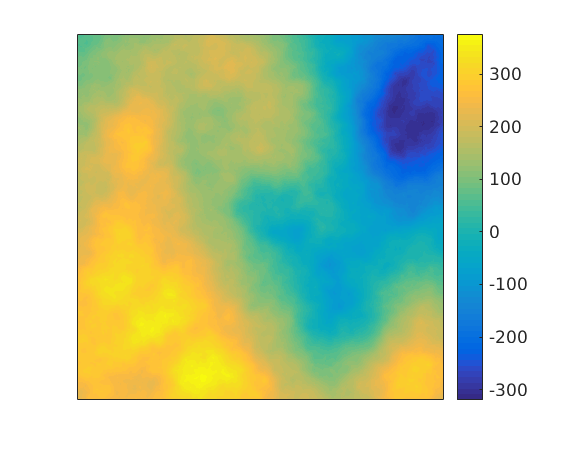
\includegraphics[width = 1.1\textwidth, height = 0.9\textwidth]{Electrostatic1}
%	\end{subfigure}
%	\begin{subfigure}[b]{\plotwidth}	
%		\centering	
%		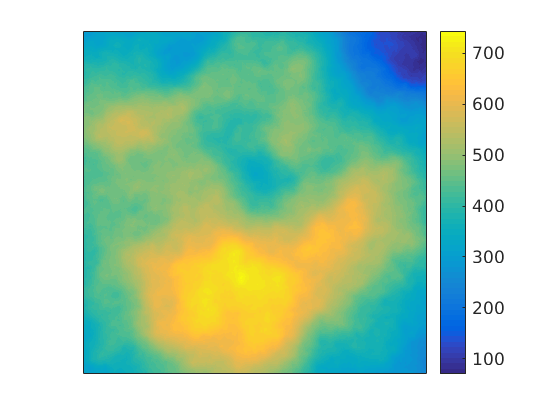
\includegraphics[width = 1.1\textwidth, height = 0.9\textwidth]{Electrostatic2}
%	\end{subfigure}
%	\begin{subfigure}[b]{\plotwidth}	
%		\centering	
%		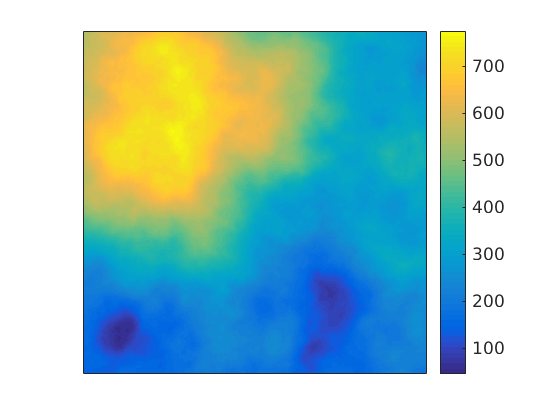
\includegraphics[width = 1.1\textwidth, height = 0.9\textwidth]{Electrostatic3}
%	\end{subfigure}
%	\caption{Electrostatic field generated by a $15 000$ randomly charged particles gas, evaluated on a $1225\times 1225$ points grid. The pre-processing needed to compute this figure was of about $50s$. After that, each one of the figures are computed in about $3s$. On the computer we used, this represented a speed-up of about a factor $2000$ (estimated by measuring the time needed to compute a proportion of the full interactions)}
%	\label{figElectrostatic}
%\end{figure}	
%
%\subsection{Self-canceling acoustic field : non-linear optimization}
%
%Consider $N_z$ punctual 2-dimensional sound sources located at $\varInRange{\bs{z}}{l}{1}{N_z}$  and emitting at a single frequency $f$, with unit amplitude and phases $\phi = \varInRange{\varphi}{l}{1}{N_z}$. That is, for each $l \in \{1,\cdots, N_z\}$, the source number $l$ generated an acoustic pressure at each point $\bs{x}$ and time $t$ in $\R^2$ equal to 
%\[p_l(\bs{x},t) = \Re\left[-\frac{i}{4}H^{(1)}(k\abs{\bs{z}_l - \bs{x}}) e^{-i\left(\omega t - \varphi_l \right)}\right],\]
%where $\omega = 2\pi f$, $k = \frac{2\pi f}{c}$, with $c$ the celerity of the sound waves, and $H^{(1)}$ is the Hankel function of first kind already defined in \autoref{HelmoholtzSubSection}. 
%By superposition, the resulting pressure at $\bs{x}$ is 
%\[p(\bs{x},t) = \Re\left[ -\frac{i}{4}e^{-i \omega t} \sum_{l=1}^{N_z} H^{(1)}(k\abs{\bs{z}_l - \bs{x}})e^{i \varphi_l} \right],\]
%and the sound intensity is proportional to
%\[\Pi(\bs{x},\varphi) =  \abs{ \sum_{l=1}^{N_z} H^{(1)}(k\abs{\bs{z}_l - \bs{x}})e^{i \varphi_l} }^2.\]
%Suppose one wishes to choose the phases that minimize the sound intensity in a prescribed zone $\Omega$, that is,
%\[ \varphi^* = \underset{\varphi \in [0,2\pi]^{N_z}}{\text{argmin}}\int_{\Omega}\Pi(\bs{x},\varphi). \]
%If we approximate the integral over $\Omega$ by a uniform quadrature, this leads to solving 
%\[\varphi^* = \underset{\varphi \in [0,2\pi]^{N_z}}{\text{argmin}} \sum_{q=1}^{Q}\Pi(\bs{x}_q,\varphi), \]
%where $\bs{x}_q$ are the coordinated of the quadrature points. Letting $A_{l,q} = H^{(1)}(k\abs{\bs{x}_q - \bs{z}_l})$ and $q(\varphi) = \left(e^{i\varphi_l}\right)_{1 \leq l \leq N_z}$, this rewrites
%\[ \varphi* = \underset{\varphi \in [0,2\pi]^{N_z}}{\text{argmin}} q(\varphi)^T A^T A ~ ~ q(\varphi).\]
%The cost function associated to this minimization problem can be evaluated rapidly, as well as its gradient. Thus, using black-box optimization procedures such as MATLAB's fmincon, we can find rapidly good candidates for $\varphi^*$. In \autoref{figMinimizationHelmholtz}, we show the result of one such optimization.  
%\begin{figure}[H]
%	\begin{subfigure}[b]{0.49\textwidth}
%		\centering
%		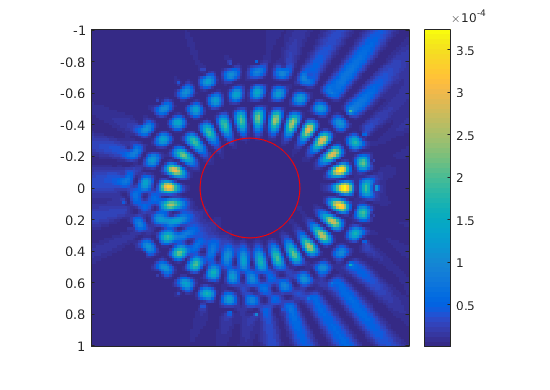
\includegraphics[width=1.15\textwidth,height=0.8\textwidth]{figHelmholtzShadow}
%	\end{subfigure}
%	\begin{subfigure}[b]{0.49\textwidth}
%		\centering
%		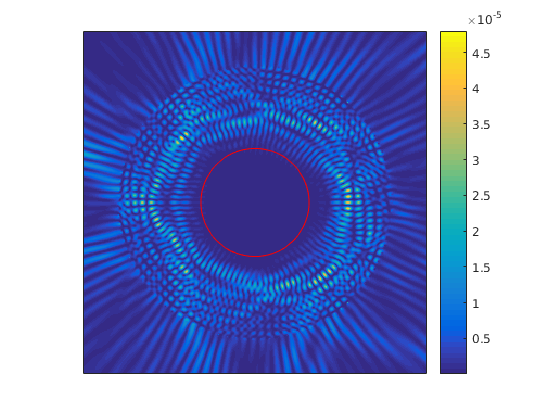
\includegraphics[width=1.15\textwidth,height =0.8\textwidth]{figHelmholtzShadow2}
%	\end{subfigure}
%	\caption{Result of the optimisation with $N_x = 500$ regularly spaced on a circle centered at the origin, with a wavenumber $k = 70$, and $\Omega$ a small circle centered on the origin, represented in red, discretized by a grid of $10^5$ points}
%	\label{figMinimizationHelmholtz}
%\end{figure}
%
%
%
%%% BIBLIO														
%\IfFileExists{biblio.bib}{\bibliography{biblio}}{\bibliography{/home/martin/Documents/These/Biblio/biblio}}
%\bibliographystyle{plain}
%																																																						
%\end{document} 